\documentclass[11pt,a4paper,openany]{book}
\input{public_payload/latex/r017_source/preamble}
% OC Core 1.4 uses the canonical display-book source contract.
\usepackage{tikz}
\usetikzlibrary{arrows.meta,positioning}
\hypersetup{pdftitle={Ontology of Continua},pdfauthor={Alexander Yashin},pdfsubject={Version 1.4 review manuscript}}
\geometry{a4paper,inner=3.2cm,outer=2.8cm,top=3.0cm,bottom=3.0cm}
\linespread{1.08}\selectfont
\setlength{\parskip}{0.42em}
% OC Core 1.4 uses a book-readable R017+ layout: roomier margins and line spacing, not content padding.
\geometry{a4paper,inner=3.1cm,outer=2.9cm,top=3.0cm,bottom=3.0cm}
\linespread{1.08}\selectfont
\setlength{\parskip}{0.45em}
\begin{document}
\frontmatter
\begin{titlepage}
\centering
\vspace*{0.08\textheight}
{\Large Ontology of Continua\par}
\vspace{0.35cm}
{\huge\bfseries A Monograph on a Universal Operational Language for Systems\par}
\vspace{0.8cm}
{\large Alexander Yashin\par}
{\normalsize Independent Researcher, Leipzig/Halle, Germany\par}
{\normalsize ORCID: 0009-0008-6166-0914\par}
\vspace{0.45cm}
{\normalsize Version 1.4\par}
{\normalsize Manuscript revision date: 14 May 2026\par}
{\normalsize Concept DOI route: 10.5281/zenodo.17899134\par}
\vfill
\begin{minipage}{0.76\textwidth}
\centering\itshape Dedicated to my dear wife Maria, without whom this work would have been impossible.
\end{minipage}
\vfill
{\small Manuscript status: review manuscript. Public release, DOI action, journal submission, and migration require explicit owner approval.\par}
\end{titlepage}
\chapter*{Opening Matter}
\addcontentsline{toc}{chapter}{Opening Matter}
\section*{Acknowledgements}
This book has been shaped by a long chain of intellectual pressure: older philosophers who made relation and becoming impossible to ignore, scientists who forced vague system talk to answer to measurement, engineers who taught that a language which cannot survive implementation is only ornament, and readers who would not accept an elegant sentence where an exact distinction was needed. None of those pressures is an endorsement of the theory. They are part of the discipline under which the manuscript was written.\par
The work is dedicated to Maria. A project of this size needs more than hours at a desk; it needs the quiet permission to return to the same question again and again until the question finally begins to answer back. That ordinary loyalty is not an appendix to the science. It is the condition under which the science became possible.\par
I also owe a debt to the stubbornness of practical work. A theory of systems that cannot be made useful near organizations, infrastructures, software, people, and material constraints has not yet earned its breadth. The manuscript carries that pressure throughout: every large claim has to become small enough to inspect, every attractive abstraction has to survive contact with a case, and every case has to admit the possibility that it may be the wrong test.\par
The acknowledgements are therefore deliberately sober. They do not ask the reader to grant authority by association; acknowledgement does not imply authorship, endorsement, or agreement with the claims. It names a more useful debt: the pressure of readers, predecessors, tools, and cases that made loose language uncomfortable. A monograph on continua should not hide the conditions of its own continuity; it should show how an idea is kept alive by criticism as much as by conviction.\par
\section*{Abstract}
Ontology of Continua is an attempt to describe the behavior of systems in a language that is formal enough to be inspected and broad enough to cross disciplinary borders without pretending that the disciplines themselves disappear. The central problem is simple to state and difficult to handle: many systems appear to preserve identity while changing, to collapse when contradiction can no longer be absorbed, or to open a new degree of freedom when the old description is exhausted. The monograph asks whether those events can be treated as instances of one operational pattern rather than as unrelated metaphors.\par
The book begins before the formalism. It first reconstructs why ontology, metaontology, general systems theory, cybernetics, complexity theory, and mathematical modeling repeatedly return to the same pressure point: a world without observed domain walls still presents us with many local vocabularies. It then introduces the motivating hypothesis in a deliberately narrow form: an unresolvable contradiction either gives rise to a new dimension of description or collapses the structure that carries it. The later chapters formalize axes, continua, operators, K-levels, proof obligations, evidence lanes, simulations, datasets, and falsification routes around that hypothesis.\par
The scientific status is conservative. A chapter may explain an idea vividly, but no prose, table, figure, or example is allowed to make a claim stronger than the proof graph, Lean-facing formalization, empirical support, comparator pressure, and review state permit. The reader is therefore invited to read the book in two ways at once: as a continuous argument about systems and as a map of what has been proved, what has been tested, what remains conditional, and what would falsify the proposal.\par
The intended payoff is not a new label for old intuitions. If the proposal works, it should help a reader translate between domains without flattening them, compare systems whose native languages are otherwise incompatible, notice when a description is missing an axis, and separate a genuine explanatory advance from a metaphor that merely travels well. If it fails, it should fail in public ways: a dependency should break, a comparison should lose its target, a dataset should refuse the claimed pattern, or a formal obligation should remain open.\par
This double demand gives the book its shape. It is not a reference manual, because the concepts have to be earned in order. It is not a popular essay, because the claims must remain traceable. It is not only a formal appendix, because the formal objects need motivation, history, rival models, and examples before their burden is clear. The intended object is a scientific monograph in the old sense: a sustained argument that teaches its own language while exposing the places where that language can be defeated.\par
\section*{Reader Orientation}
The intended reader may be a philosopher, mathematician, physicist, systems engineer, enterprise architect, complexity researcher, or simply a careful person willing to follow a hard problem without accepting slogans. The opening chapters assume no membership in the project. Terms are introduced before they are used. Authors and schools are named with enough context to explain why they matter. When a figure appears, the surrounding prose says what it clarifies; when a table appears, the text says what may and may not be inferred from it; when an equation appears, it is attached to a local dependency rather than displayed as decoration.\par
The route is intentionally sequential. First comes the historical and conceptual pressure: why a universal operational language for systems became a plausible thing to seek. Then comes motivation: what present models often leave unmeasured, and why that absence matters outside academic classification. Then comes intuition: the absence of observed domain walls, the distinction between a principle and its domain projections, and the question of dimensional birth. Only after that does the book turn to the formal core, the hierarchy of continua, theorem and proof surfaces, Lean-facing constraints, empirical examples, comparators, falsifiers, and reproducibility.\par
The reader does not need to agree quickly. In fact, the book is written against premature agreement. The most useful reader is the one who keeps asking: where did this entity enter, what supports it, what would break it, what would a rival model say, and what practical decision changes if the proposed language works. Those questions are not interruptions. They are the reading method the monograph expects.\par
A second route is available for readers who come to the book with a technical question already in hand. They may move from the conceptual chapters to the formal spine, from there to proof and evidence surfaces, and finally into the appendices where reproducibility and boundary conditions are gathered. That route is faster, but it is not meant to excuse the historical and motivational chapters. Those early chapters are where the book earns the right to ask for a universal language in the first place.\par
The front matter is meant to be navigable as well as ceremonial: it gives the contents, the list of figures, and the list of tables before the main argument begins. Those lists are not decorative inventories. They show where the book asks a diagram, a quantitative comparison, or a worked example to carry part of the reader's inspection.\par
The book also tries to remain hospitable to machine reading. That does not mean flattening the prose into labeled fields. It means making the order of introduction explicit, keeping claims close to their support, using captions that say what an object does in the argument, and avoiding theatrical mystery where a simple definition would serve. A human reader can feel guided; a machine reader can find the same route recoverable.\par
\section*{Scientific Status And Claim Discipline}
The monograph distinguishes exposition from certification. Exposition makes a claim understandable; certification says what kind of support the claim currently has. The two are related, but they are not the same. A polished paragraph can make an unresolved idea easier to inspect, yet it cannot turn that idea into a theorem. A figure can show how a dependency is organized, yet it cannot replace proof. A numerical example can teach scale, yet it cannot stand in for a dataset unless it is explicitly bound to one.\par
For that reason, the book keeps several forms of support separate: definitions and formal objects, theorem statements, proof sheets, Lean-facing declarations, finite checks, datasets, simulations, evidence executions, comparator discussions, falsification conditions, and reviewer objections. The reader can move from any public claim to the scientific object that carries it. Where the object is not closed, the claim remains conditional. That restraint is not modesty for style; it is a structural requirement of the work.\par
The restraint also protects the interesting part of the theory. A universal language is tempting precisely because it can make distant domains sound alike. The danger is that the likeness may be verbal rather than structural. The book therefore treats each domain projection as a test of translation: what is retained, what is lost, which quantity changes, which rival description would explain the same case more cheaply, and what observation would make the proposed reading collapse.\par
Readers should expect three kinds of statements. Some are definitions: they say how a term is used in this work. Some are claims under support: they are tied to proof, evidence, or comparison. Some are conjectural or programmatic: they point to work that remains open. The book tries to keep these kinds apart even when the prose is continuous, because confusing them would make the theory look stronger and less useful at the same time.\par
\section*{Notation And Glossary Route}
Notation enters gradually. The book does not begin by dropping symbols on the reader and asking for trust. It first establishes why axes are needed, why a continuum is not merely a smooth interval, why operators carry explanatory burden, and why a hierarchy of continua is required before cross-domain comparison becomes meaningful. Symbols such as support, loss, threshold, residual, projection, obligation, lane, and closure are introduced in local use and gathered again in the appendices.\par
The formal notation has one job: to make disagreement more precise. If a formula appears, the surrounding passage explains which dependency it names. If a table appears, it tells the reader which quantity, case, or comparison is being held steady. If a footnote appears, it should clarify a term, preserve a caveat, or place a predecessor in context without breaking the rhythm of the main line. The aim is not to make the book look rigorous; it is to make the rigor inspectable.\par
The same rule applies to examples. A small number is not presented as a grand measurement; it is a way of showing how a claim behaves under pressure. A worked case is not a proof; it is a route through a claim that lets the reader see where the claim would fail. The book uses these devices because a theory of systems must be readable at several scales: as a philosophical argument, as a formal apparatus, as a scientific research program, and as something a careful practitioner could attempt to test on a real situation.\par
The appendices collect the slower routes: terminology, proof references, evidence families, comparator notes, and reproducibility surfaces. They are not a warehouse for material that did not fit the book. They are a second reading layer for anyone who wants to audit the argument rather than merely follow it. The main text therefore remains readable, while the technical trail remains available. That division is part of the promise of the edition: clarity first, then auditability without concealment, and finally enough redundancy that a careful critic can reconstruct the route independently.\par
\tableofcontents
\renewcommand{\listfigurename}{List of Figures.}
\listoffigures
\renewcommand{\listtablename}{List of Tables.}
\listoftables
\clearpage
\mainmatter
\part{introduction}
\chapter{What This Monograph Is}
\section{The Local Problem In Monograph Is}
Many systems matter most at the point where their description begins to move. A body heats, cools, breaks, and mixes. A living organism maintains itself by exchanging matter and energy with what is not itself. A scientific field changes when an old distinction no longer separates the important cases from the unimportant ones. A political institution preserves some rules, abandons others, and may fail when the tensions it was built to carry exceed the forms available to it. These are not instances of one substance, one law, or one science. They do not share instruments, variables, evidence, or standards of explanation. Yet each forces a related difficulty: how is a system to be described when its boundaries, relevant contrasts, and modes of operation are among the things that change? \cite{landau_stat_physics,prigogine_dissipative}\par
The difficulty is easy to miss because ordinary description often works by stabilizing its object before it begins. One names the thing, draws a boundary around it, assigns it properties, and then studies what happens. Much of the time this is not only legitimate but necessary. A measurement must decide what is being measured. An experiment must establish a difference between system and environment. A legal rule must say where its authority begins and ends. A biological account must distinguish organism, organ, cell, and medium. Without such distinctions, nothing precise can be said.\par
The next diagram slows the argument down just enough to show how monograph is is being organized.\par
\begin{figure}[htbp]
\centering
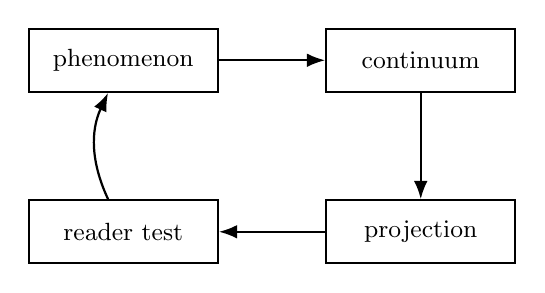
\begin{tikzpicture}[node distance=1.35cm,>=Latex,every node/.style={font=\small}]
\node[draw,thick,align=center,minimum width=2.4cm,minimum height=0.8cm] (a) {phenomenon};
\node[draw,thick,align=center,minimum width=2.4cm,minimum height=0.8cm,right=of a] (b) {continuum};
\node[draw,thick,align=center,minimum width=2.4cm,minimum height=0.8cm,below=of b] (c) {projection};
\node[draw,thick,align=center,minimum width=2.4cm,minimum height=0.8cm,left=of c] (d) {reader test};
\draw[->,thick] (a) -- (b);
\draw[->,thick] (b) -- (c);
\draw[->,thick] (c) -- (d);
\draw[->,thick,bend left=25] (d) to (a);
\end{tikzpicture}
\caption{Monograph Is: concept map of conceptual dependency pressure 6-1-1}
\label{fig:figure-what-this-monograph-is-one}
\end{figure}
The point of the diagram is not decoration; it marks which relation is being proposed and which stronger conclusion is still unavailable.\par
A local clarification is useful here\par
A local clarification is useful here\footnote{In Monograph Is, this note clarifies the reader clarification role of the term and keeps the caveat close to the sentence that needs it.}.\par
The note keeps the caveat near the term without derailing the main sentence.\par
The trouble begins when the distinction that made precision possible also becomes part of the process under study. A membrane is not simply a line around a cell; it is an active condition of exchange. A scientific concept is not simply a label; it determines what counts as a case, an anomaly, or a result. A constitutional procedure is not merely an external description of an institution; it is one of the ways the institution acts. In such cases, the boundary is not a neutral container. It belongs to the behavior that must be understood.\par
An ordinary physical scene already shows the problem. A pot of water on a stove may be described as water in a vessel receiving heat. For some purposes that is enough. A thermometer supplies a temperature. The flame or electric element supplies energy. The pot separates the water from the stove and the room. But as the process continues, the description has to become more differentiated. Bubbles form. Vapor leaves the surface. Convection appears. If salt is added, the relevant variables change. If a lid is placed on the pot, pressure and exchange with the room change. The same object has not vanished, but the useful description has shifted. The boundary that mattered for one question is not necessarily the boundary that matters for the next.\par
A living example makes the point without borrowing its force from heat. Consider a wound healing on the surface of an organism. At one scale, the wound is a break in tissue. At another, it is a changing field of clotting, inflammation, cell migration, chemical signaling, microbial risk, and mechanical stress. The boundary of the wound is visible, but it is also biochemical and temporal. What counts as repair changes as the process moves from sealing to inflammation, from inflammation to tissue formation, from tissue formation to remodeling. A description that treats the wound as a fixed gap in a surface misses the sequence by which the organism re-establishes a functional boundary. A description that lists only molecules misses the organized repair of tissue. The case requires levels without allowing any level to pretend that it owns the whole event.\par
Scientific concepts undergo a comparable pressure in another register. The word gene did not retain a single stable content from classical genetics through molecular biology and into contemporary genomics. It carried inheritance, then sequence, then regulation, expression, interaction, and context. The older word did not simply disappear, nor did it remain untouched. It was forced to carry distinctions that earlier use could not adequately hold. Here the changing system is not a pot or a tissue but a field of inquiry. Its objects, methods, and contrasts are reorganized together. The concept survives by acquiring new dimensions of description.\par
This monograph develops a vocabulary for such cases. It treats OC Core 1.4 as an operational metaontology: a disciplined language for comparing descriptions of systems without pretending that one domain supplies the final language for all the others. Ontology, in this use, names the kinds of things a description allows itself to speak about. Metaontology names the comparison of such vocabularies. Operational means that the comparison must remain tied to describable acts: drawing a boundary, stating a dimension of variation, applying a transformation, moving between levels, and accounting for what is preserved or lost in that movement.\par
The ambition is therefore narrower than a universal theory and wider than a local technical glossary. OC does not reduce biology to physics, institutions to organisms, or concepts to thermodynamic processes. It does not treat analogy as evidence. Its concern is the disciplined statement of changing descriptions: what varies, what holds, what crosses a boundary, what operation changes the configuration, and when a description must acquire a new axis or give way. The monograph begins here because before formal notation or extended examples can do useful work, the reader must know what kind of object is being offered.\par
\section{The Necessary Distinction In Monograph Is}
Modern inquiry already depends on layered description. A gas may be approached through molecular motion, statistical distributions, or macroscopic variables such as pressure, volume, and temperature. Landau and Lifshitz, in their treatment of statistical physics, make this layered relation central: microscopic multiplicity and macroscopic regularity are connected, but not collapsed into the same descriptive act. The difference between levels is part of the science, not an embarrassment to it. \cite{landau_stat_physics,prigogine_dissipative}\par
Open and structured systems intensify the problem. Ilya Prigogine's work on dissipative structures showed how order can arise in systems maintained by flows of energy and matter. Nicolis and Prigogine developed this insight through self-organization, instability, and fluctuation. Hermann Haken's synergetics studied the appearance of collective order through variables that coordinate many components at once. These bodies of work do not establish OC. They provide a neighboring pressure: serious accounts of changing systems often need languages for level, transition, constraint, instability, and emergent order.\par
The local dependency can now be written without changing the claim it supports.\par
\begin{equation}\label{eq:equation-what-this-monograph-is-two}
\operatorname{boundaryResidual}_{1} = C_{\mathrm{unres}}=\min_{\pi\in\Pi}\|B(x)-B(\pi x)\|
\end{equation}
The relation names a local dependency, variable dictionary, and proof/evidence role; it is not a claim-status upgrade.\par
The formula is a restraint on the prose. It names the dependency that the surrounding paragraph is allowed to use.\par
The comparison below gives monograph is a set of quantities that can be inspected instead of merely admired.\par
\begin{table}[htbp]
\centering\small
\caption{Monograph Is: observable quantities and counter-pressure 6-2-1}
\label{tab:table-what-this-monograph-is-one}
\begin{tabular}{@{}llll@{}}
\toprule
Boundary & Measured cue & Scale & Failure sign \\
\midrule
monograph is boundary & 12 units & declared case & fixes what is compared \\
residual pressure & 0.28 & dimensionless & shows unresolved load \\
projection loss & 0.44 & bounded interval & marks lost structure \\
countercase set & 9 cases & review sample & keeps a falsifier visible \\
\bottomrule
\end{tabular}
\end{table}
The table should be read locally: it narrows the comparison without pretending that the wider theory has been settled by a single surface.\par
The distinction is important. Precedent is not proof. Analogy is not evidence. Motivation is not validation. Scientific work on thermodynamics, self-organization, and collective order shows that certain descriptive pressures are real within established domains. It does not show that a proposed metaontological vocabulary is necessary, sufficient, or correct. OC must earn its value by making descriptions clearer than they would otherwise be, by refusing illegitimate transfers between domains, and by exposing places where its own terms fail to constrain a claim.\par
The need appears whenever a word moves too easily across levels. A cell is composed of molecules, but a cell is not merely a molecule made large. Its boundary, metabolism, repair, and reproduction matter at an organized level that cannot be recovered by naming parts alone. An institution is made of persons and artifacts, but it is not a person. Its procedures, offices, records, permissions, and sanctions have forms of continuity no individual body possesses. A model may represent a process, but it is not the process. To confuse these levels is not simply to make a philosophical mistake; it can damage explanation.\par
There are two common escapes from this difficulty. One is flattening. Everything is translated into the favored language of one scale, and the rest is treated as derivative or rhetorical. The other is isolation. Every field retains its own vocabulary so completely that comparison becomes impossible except as metaphor. OC attempts a middle path. It asks for comparison without flattening and difference without isolation. That path requires terms that are general enough to travel but strict enough to resist decorative use.\par
The first of these terms is continuum. A continuum is a dimension of describable variation. Temperature is an obvious physical example, but the notion is not restricted to smooth numerical scales. Viability in an organism, legitimacy in an institution, confidence in a model, or resolution in a conceptual dispute may each function as an ordered field of difference if the ordering is stated with enough care. Some continua are measurable with instruments. Some are qualitative but still constrained. Some are formal. The point is not to make them equal; it is to require that variation be named rather than smuggled into a fixed category.\par
A boundary is the condition by which a system, state, level, or description is separated from what is not being treated as part of it. The boundary may be physical, as in a membrane or vessel. It may be formal, as in the separation between variables in a model. It may be methodological, as in an experimental protocol. It may be institutional, as in a rule that distinguishes office from person. Boundaries can hold, move, leak, fail, or be redrawn. A description that cannot say what boundary it uses usually cannot say what its claim is about.\par
An operator is a named transformation. Heating, cooling, sealing, stirring, and adding solute are operators in a simple physical example. Cell division, immune response, repair, inhibition, and signaling may function as operators in biological description. In conceptual inquiry, an operator may be a definition, a classification, a measurement procedure, or an inference rule. In an institution, it may be a vote, appointment, veto, sanction, or transfer of authority. The term remains disciplined only if the operation specifies what it acts upon and what kind of change it produces.\par
A projection is a mapping from one descriptive frame into another. Projection is unavoidable because no account preserves everything. A thermodynamic description does not preserve the individuality of every molecule. A statistical description of a population does not preserve the biography of every member. A legal description of an office does not preserve the private motives of the person occupying it. Projection becomes dangerous when its losses are hidden. OC treats loss and distortion as part of the description, not as defects to be concealed.\par
These terms have practical value before they have formal elegance. They help state where a claim begins and ends. They distinguish a system from the variables chosen to describe it. They ask whether a boundary is physical, conceptual, methodological, institutional, or formal. They separate evidence from analogy by requiring a projection to say what is preserved. They allow a conflict to be examined as noise, external disturbance, manageable tension, or pressure that demands a new descriptive dimension. None of this solves the sciences or the humanities. It supplies a common discipline for describing the movement between descriptions.\par
\section{The Testable Step In Monograph Is}
The central habit of OC is to treat systems through organized continua rather than through fixed categories alone. Fixed categories remain indispensable. A thing often must be called liquid rather than solid, alive rather than dead, valid rather than invalid, authorized rather than unauthorized. But many of the most important cases occur near thresholds, across transitions, or within mixed conditions. A living tissue may be injured but repairing. A scientific concept may be unstable but not abandoned. An institution may remain legally continuous while losing the capacity to coordinate action. The fixed name remains, yet the relevant variation has become decisive. \cite{landau_stat_physics,prigogine_dissipative}\par
A continuum does not erase difference. It organizes difference. It asks what can vary, along what axis, within what limits, under what constraints, and by what operations. Temperature, concentration, density, entropy, probability, confidence, viability, stability, authority, and legitimacy are not the same kind of thing. They should not be made to look alike by verbal force. But each can become a dimension along which a system is described as more or less, nearer or farther, stable or unstable, viable or nonviable, resolved or unresolved. OC begins from the disciplined use of such dimensions.\par
The local dependency can now be written without changing the claim it supports.\par
\begin{equation}\label{eq:equation-what-this-monograph-is-one}
\operatorname{axisInformation}_{1} = \Delta d=\operatorname{rank}(A_{\mathrm{new}})-\operatorname{rank}(A_{\mathrm{old}})
\end{equation}
The relation names a local dependency, variable dictionary, and proof/evidence role; it is not a claim-status upgrade.\par
The formula is a restraint on the prose. It names the dependency that the surrounding paragraph is allowed to use.\par
The local dependency can now be written without changing the claim it supports.\par
\begin{equation}\label{eq:equation-what-this-monograph-is-three}
\operatorname{projectionLoss}_{1} = P_{\mathrm{collapse}}=\sigma(\alpha R-\beta S-\gamma M)
\end{equation}
The relation names a local dependency, variable dictionary, and proof/evidence role; it is not a claim-status upgrade.\par
The formula is a restraint on the prose. It names the dependency that the surrounding paragraph is allowed to use.\par
A small numerical test keeps the abstraction honest at the scale of a single decision.\par
\paragraph{Numerical example.} For monograph is, take support=0.45, projection loss=0.11, and 2 open obligations. The bounded score is 0.113; the example gives the reader a numeric scale without pretending to be empirical proof.\par
The numbers are deliberately small; their value is pedagogical, not evidential, unless the chapter binds them to a dataset elsewhere.\par
The pot of water can now be left in its proper place: useful, but limited. It shows that a physical system may require different boundaries and variables as it changes. It does not show that all systems are thermal systems. It does not give laws for societies or concepts. It gives only a clear case in which the adequacy of description depends on phase, exchange, constraint, and operation. Its lesson is methodological: a system's identity under description is tied to the question being asked and the transformation being considered.\par
The biological wound gives a richer sense of the same methodological demand. At first glance, the wound is a defect in a surface. Yet the organism does not merely fill a hole. It initiates clotting, recruits immune activity, clears damaged matter, produces new tissue, and remodels structure over time. The relevant boundary is not fixed at the visible edge of the wound. It is enacted by processes that distinguish inside from outside, self from threat, damaged from viable, temporary repair from restored function. A description that treats healing as a single event misses the ordered transformation by which the system recovers a boundary.\par
In that case, the operator is not one action but a sequence of transformations. Clotting, inflammation, proliferation, and remodeling each change the configuration. The continuum of concern also shifts. At one moment bleeding versus sealing is decisive. Later, infection risk, tissue strength, scar formation, and restored function become more important. The system remains the organism, or the tissue, or the wound site, depending on the level of analysis. Each choice is legitimate only if its boundary and variables answer to the question being asked.\par
Scientific concept change offers a second non-physical pressure. When a field inherits a term that no longer separates its cases adequately, the term may be abandoned, narrowed, split, or expanded. The concept of species, for example, has been treated through interbreeding, morphology, lineage, ecological niche, genetic clustering, and evolutionary history. No single formulation has erased the others for every purpose. The concept persists because different continua become relevant in different inquiries. The difficulty is not merely verbal. Classification affects measurement, conservation, evolutionary explanation, and the comparison of organisms across time.\par
Here the boundary is conceptual and methodological. What counts as the same species depends on the operation by which sameness is being tested. Reproductive isolation, genetic distance, morphological continuity, and phylogenetic relation do not always yield identical partitions. The conflict among them is not automatically a contradiction in the strongest sense. Often it is a plurality of legitimate projections. But when a field requires one classification to do work that its own criteria cannot support, the tension becomes more severe. The concept must gain a new dimension, accept limited scope, or fail in that use.\par
This is where the hypothesis of OC begins to take shape. Some tensions can be managed within an existing description. Some are local errors, bad measurements, or ambiguous cases. Some mark the ordinary plurality of purposes. But some tensions press against the descriptive space itself. The available dimensions cannot jointly carry the commitments being made. When that happens, the system under description tends toward one of two broad outcomes: it acquires or requires a new dimension of description, or the configuration organized by the old description loses its capacity to hold.\par
The word contradiction is reserved for this stronger case. It does not mean every disagreement, inconvenience, opposition, or anomaly. It means a tension within a configuration such that the active commitments cannot continue together without alteration, expansion, or breakdown. The contradiction may be logical, formal, institutional, conceptual, or operational, depending on the domain. In a physical case, the term must be used with care, because phase transition is not a quarrel inside matter. In a conceptual or institutional case, the word may be closer to ordinary use, but it still requires specification.\par
Dimension also needs restraint. A new dimension is not any new word added to a description. It is an axis of relevant difference that was previously absent, suppressed, or treated as secondary but becomes necessary for the claim to remain adequate. A policy dispute that appears to involve only cost may reveal that risk, time, trust, jurisdiction, or legitimacy is part of the real structure. A scientific classification that appears to involve only surface form may require lineage or mechanism. A healing wound that appears to involve only closure may require viability and function. In each case, the description changes because the prior terms cannot do enough work.\par
Collapse is the other possibility. Collapse does not always mean destruction. A model collapses when its assumptions no longer support the claims made through it. A category collapses when it can no longer separate the cases it was supposed to distinguish. An institution collapses when its procedures no longer coordinate authority and action, even if buildings, documents, and titles remain. A physical arrangement collapses when sustaining constraints fail. The common feature is loss of organization relative to the description in use.\par
The concept of OC therefore depends on a double discipline. It must be generous enough to follow changing systems across levels, but strict enough to say when a proposed description has failed. A continuum must state its variation. A boundary must state its separation. An operator must state its transformation. A projection must state its preservation and loss. A contradiction must state why the current descriptive dimensions cannot carry the commitments assigned to them. Without these requirements, the vocabulary would become ornamental. With them, it can become a testable way of arranging questions.\par
\section{An Objection Worth Keeping In Monograph Is}
The formal vocabulary of the monograph grows from these pressures rather than preceding them. A system is a bounded configuration under description. The phrase under description matters. It does not imply that the system is invented by the observer, nor that reality waits for vocabulary in order to exist. It means that every inquiry approaches a system through selected boundaries, variables, instruments, purposes, and levels. The system may resist the description. That resistance is one reason the description must be explicit. \cite{landau_stat_physics,prigogine_dissipative}\par
A boundary is the operative separation that makes a system describable. In some cases the boundary is a material surface: membrane, wall, vessel, skin. In others it is a threshold, rule, convention, interface, legal distinction, model assumption, or measurement decision. The same real process may have several legitimate boundaries depending on the operation at stake. In the wound, the visible tear, the immune field, the microbial interface, and the functional tissue boundary are not identical. Treating one as if it were all the others produces confusion.\par
A small numerical test keeps the abstraction honest at the scale of a single decision.\par
\paragraph{Numerical example.} For monograph is, take support=0.48, projection loss=0.16, and 3 open obligations. The bounded score is 0.; the example gives the reader a numeric scale without pretending to be empirical proof.\par
The numbers are deliberately small; their value is pedagogical, not evidential, unless the chapter binds them to a dataset elsewhere.\par
The case that follows turns the proposal into a sequence of criticizable moves.\par
\paragraph{Worked case.} In the worked case for monograph is, the claim is reduced to a boundary, an observable, a dependency, a numerical cue, and a falsifier. The case is useful only because each move can be criticized separately.\par
The case helps because each step can fail separately, which is exactly what a useful example should permit.\par
A continuum is an ordered field of possible variation relevant to the system. The ordering may be numerical, ordinal, qualitative, formal, or practical. A continuum is not valid merely because a noun has been turned into a scale. It must say what changes and why the change matters. Temperature, concentration, and pressure have established measurement procedures in physics. Viability, legitimacy, and confidence require different forms of discipline. OC permits them to be discussed under the shared notion of ordered variation, but it does not pretend that their evidentiary status is the same.\par
A state is a located condition within one or more continua. It is not always a point in a mathematical space, though later formalization may represent it that way for selected purposes. A state may be approximate, distributed, unstable, or dependent on measurement. The relevant question is what condition is being attributed to the system at a given level of description. Liquid water near boiling, inflamed tissue in repair, a disputed scientific category, and an institution in procedural deadlock are all states only relative to the continua and boundaries being used.\par
An operator is a transformation that acts on a state, boundary, continuum, relation, or projection. The word is intentionally broad because transformations differ across domains. But breadth does not remove obligation. An operator must identify its target and effect. Heating changes thermal state. Sealing changes exchange. A definition changes classification. A measurement procedure changes what can count as data. A vote changes institutional authorization when rules make it effective. If the target and effect cannot be stated, the operator has not been specified.\par
A projection is a mapping between descriptions. It allows one account to be expressed through another, or one level to be related to another, without pretending that nothing is lost. Projection is central because every cross-level or cross-domain statement selects. A molecular account projected into thermodynamic variables preserves some aggregate relations and loses individual histories. A clinical account projected into a public health statistic preserves population patterns and loses singular experience. A theory of institutions projected into a formal model preserves certain relations and leaves out many motives, contingencies, and meanings. The losses are not always defects. They are the price of the description, and they must be named.\par
Hierarchy of continua names the fact that continua may be organized across levels. A molecular continuum may concern kinetic distributions. A thermodynamic continuum may concern temperature. A biological continuum may concern viability, repair, or reproduction. A conceptual continuum may concern scope, precision, or explanatory power. A social continuum may concern authority, trust, compliance, or conflict. Higher-level continua may depend on lower-level processes without being identical to them. OC uses hierarchy to keep dependence visible while avoiding premature reduction.\par
Emergence is used in a restrained sense: the appearance of a stable or describable pattern at one level that is not adequately captured by listing lower-level parts alone. This use is compatible with scientific traditions concerned with self-organization and collective order, including the work of Prigogine, Nicolis, and Haken, but compatibility is not validation. The term does not license mystery. It marks a demand for an account of how level-specific description becomes necessary.\par
Contradiction and collapse complete the opening vocabulary. A contradiction is a tension the current descriptive frame cannot carry without alteration or failure. Collapse is the loss of a configuration's capacity to maintain the organization required by the description in use. The two terms are related but not identical. A contradiction may lead to refinement rather than collapse. A collapse may occur from external shock without revealing a deep contradiction in the prior description. The relation between them has to be argued case by case.\par
Notation will later shorten these relations, but notation cannot substitute for them. A symbol for a system is only useful if the boundary has been stated. A symbol for an operator is only useful if the transformation has been named. A symbol for a projection is only useful if preservation and loss are explicit. Formal expression can reduce equivocation, reveal hidden assumptions, and make consequences inspectable. It cannot by itself make a vague claim precise. The prose commitments come first because they are what the symbols must answer to.\par
The controlling questions are ordinary even when the later apparatus becomes technical. What is the system? Where is the boundary? Which continua are active? What state is being attributed? What operator is being applied? What changes and what remains invariant? What is being projected from one description into another? What is lost in that projection? Where could the claim fail? These questions are not preliminary exercises to be discarded once the vocabulary is learned. They are the discipline that keeps the vocabulary from floating free.\par
\section{The Result Of This Passage In Monograph Is}
A language broad enough to speak about physics, biology, concepts, and institutions risks becoming too broad to constrain anything. That is the strongest danger. If every change is called an operator, every difference a continuum, every tension a contradiction, and every failure a collapse, OC would add names without adding understanding. The objection cannot be avoided by confident tone. A metaontology that cannot reject a bad description is only a style. \cite{landau_stat_physics,prigogine_dissipative}\par
The answer lies in operational constraint. A proposed continuum must state what varies. A proposed boundary must state what it separates and under what operation it matters. A proposed operator must state what it transforms. A proposed projection must state what it preserves and what it loses. A proposed contradiction must state why the current dimensions are inadequate rather than merely inconvenient. These requirements make it possible for an OC description to fail. That possibility is essential. A language that cannot fail cannot clarify.\par
The second danger is the confusion of analogy with evidence. A pot, a wound, a concept, and an institution can all be discussed in terms of boundaries and transformations. That does not mean they obey the same laws. An institution does not boil. A concept does not heal. A tissue does not hold an election. When words such as pressure, transition, repair, and collapse cross domains, they must be re-specified or treated as metaphors. OC permits comparison of descriptive structure only where the comparison is limited and the projection is explicit.\par
An institutional example shows both the use and the danger. A constitutional court may be described as part of a bounded institutional system. Its procedures operate on disputes, statutes, precedents, and claims of authority. Legitimacy may be treated as a continuum relevant to stability, but it is not temperature, not energy, and not a hidden physical force. The court may face a tension between legal continuity and public acceptance. If ordinary procedures can absorb the tension, no new dimension is required. If they cannot, the description may have to include dimensions previously treated as external: enforcement capacity, political recognition, temporal delay, or competing authority. This is not evidence of an OC law. It is a disciplined way to state what would need to be examined.\par
The third danger is formal overstatement. Because the monograph later introduces notation and mathematical surfaces, it may appear to promise the certainty associated with formal systems. That promise would be false. Formalization can clarify relations, stabilize definitions, and expose consequences. It can show that a claim is coherent under stated assumptions or incoherent under them. It cannot establish by itself that the world supplies the described structure. Evidence, simulation, historical comparison, experimental result, and domain-specific interpretation remain separate burdens.\par
The fourth danger is false novelty. Continua, boundaries, operations, projection, emergence, and collapse have long histories. They belong to mathematics, physics, biology, systems theory, cybernetics, philosophy, social theory, and many technical practices. The monograph does not ask the reader to forget those histories. Its claim is architectural in a modest sense: it arranges selected ideas into a vocabulary for describing systems whose relevant dimensions, boundaries, and transformations may themselves change. The arrangement has value only if it improves the statement, comparison, and criticism of claims.\par
A further limit concerns domain authority. OC is not a substitute for physics when the question is physical, for biology when the question is biological, for legal scholarship when the question is legal, or for historical inquiry when the question is historical. It can help state how a description is being organized, where a projection occurs, and what kind of transition is being claimed. It cannot supply the missing measurements, documents, experiments, or interpretations that a domain requires. Its use is preparatory and comparative, not sovereign.\par
There is also a limit in the treatment of contradiction. The word is powerful and therefore easily abused. Many tensions are ordinary tradeoffs. Many apparent contradictions are artifacts of bad wording. Many anomalies vanish under better measurement. Many plural classifications are legitimate because different operations are being performed. OC becomes useful only when it distinguishes these cases from situations in which the current descriptive space cannot carry its own commitments. The burden is on the analysis to show that stronger condition.\par
The scientific modesty of the monograph can be stated once, and it governs everything that follows. OC is a proposed language for disciplined description under change. It is not a completed empirical science, not a universal solvent, and not a guarantee that a difficult system has been understood. Its claims must earn their status through definition, formal treatment, example, evidence where available, comparison with alternatives, and clear failure conditions. The vocabulary opens work; it does not finish it.\par
\section{The Local Problem In Monograph Is isS06}
What this monograph offers is a way of speaking carefully when fixed categories are not enough. It begins from systems whose description changes because the system changes, because the boundary matters, because the relevant variables shift, or because the act of classification becomes part of the process. Physical transitions, biological repair, conceptual revision, and institutional strain do not become the same thing. They become comparable only in the limited sense that each can force attention to boundary, variation, operation, level, and projection. \cite{landau_stat_physics,prigogine_dissipative}\par
The opening hypothesis is deliberately held as a hypothesis. When a configuration cannot resolve a tension within its current descriptive dimensions, it tends either to require a new dimension of description or to lose the organization that made the old description adequate. This claim is not secured by naming it. It must be narrowed, formalized, tested where possible, and abandoned where it overreaches. Its value will depend on whether it helps distinguish manageable variation from deeper descriptive failure.\par
Several anchors can be carried forward. A system is a bounded configuration under description. A boundary is the operative separation that makes the system describable. A continuum is an ordered field of relevant variation. A state is a located condition within one or more continua. An operator is a named transformation. A projection is a mapping between descriptions that must account for preservation and loss. A contradiction is a tension the current descriptive frame cannot carry without alteration or failure. Collapse is the loss of organization relative to the description in use.\par
These anchors do not settle the theory. They make it readable. They also make it vulnerable in the right way. A reader can be able to ask, at every later point, whether the boundary has been stated, whether the continuum is real enough for the claim being made, whether the operator has been specified, whether the projection hides its losses, and whether the alleged contradiction is stronger than ordinary complexity. If the answer is no, the language has failed in that place.\par
The monograph therefore begins neither with a declaration of mastery nor with a retreat into isolated examples. It begins with the need for a disciplined passage between descriptions. Changing systems often require more than fixed names, but they do not excuse vague speech. The task is to keep both truths in view: domains differ, and comparison is still possible; formalization can clarify, and evidence remains separate; boundaries are chosen, and some choices are better than others; a system may persist, yet the language adequate to it may have to change.\par
The chapters that follow develop this opening vocabulary into a fuller account of hierarchy, formal expression, evidence, projection, and limit. The present chapter has a simpler role. It says what kind of work the monograph undertakes: not the replacement of existing disciplines, not the discovery of a single law beneath all change, but the construction of a careful language for systems whose own terms of description are part of their movement.\par
\chapter{Why a Universal Language of System Behaviour Is Needed}
\section{The Local Problem In Universal Language of System}
On a winter morning, a hospital emergency department can look orderly from the corridor while already beginning to fail. The lights are on. The doors open and close. Screens refresh. Clinicians move quickly between beds. The public sign outside still says emergency. Yet inside, the pattern that makes the place work may be under strain. Ambulances are arriving faster than rooms can be cleared. Laboratory results are delayed. Oxygen demand is rising. A patient who would normally be seen in minutes waits an hour. The hospital has not disappeared, but the organization that lets people, equipment, information, and judgment become care is being tested. \cite{prigogine_dissipative,haken_synergetics}\par
This kind of situation is now familiar far beyond hospitals. Modern knowledge is crowded with systems that behave intelligibly inside one discipline and obscurely at the border of another. A cell, a market, a climate regime, a software platform, a city, and an institution are not the same kind of object. They do not share the same units, instruments, clocks, or failure modes. Yet each can maintain itself, absorb disturbance, change organization, amplify small differences, and sometimes collapse. The difficulty is not that these systems are mysterious in every respect. The difficulty is that their descriptions usually become local exactly where comparison becomes necessary.\par
The next diagram slows the argument down just enough to show how universal language of system is being organized.\par
\begin{figure}[htbp]
\centering
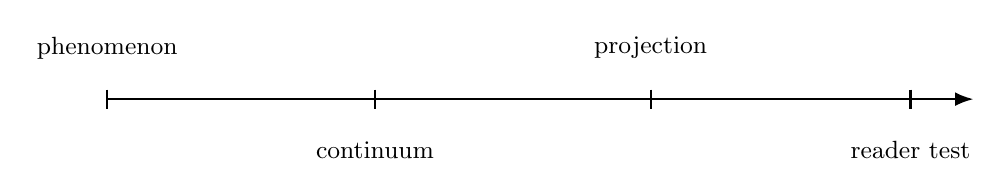
\begin{tikzpicture}[node distance=1.35cm,>=Latex,every node/.style={font=\small}]
\draw[->,thick] (0,0) -- (11,0);
\node[align=center] at (0,0.65) {phenomenon};
\node[align=center] at (3.4,-0.65) {continuum};
\node[align=center] at (6.9,0.65) {projection};
\node[align=center] at (10.2,-0.65) {reader test};
\foreach \x in {0,3.4,6.9,10.2} \draw[thick] (\x,0.12) -- (\x,-0.12);
\end{tikzpicture}
\caption{Universal Language of System: historical timeline of conceptual dependency pressure 7-1-2}
\label{fig:figure-why-a-universal-language-of-system-behaviour-is-needed-one}
\end{figure}
The point of the diagram is not decoration; it marks which relation is being proposed and which stronger conclusion is still unavailable.\par
A local clarification is useful here\par
A local clarification is useful here\footnote{In Universal Language of System, this note clarifies the reader clarification role of the term and keeps the caveat close to the sentence that needs it.}.\par
The note keeps the caveat near the term without derailing the main sentence.\par
A system, in the broad sense needed here, is an organized configuration whose parts and relations make a difference to what it can do. A behavior is a change, persistence, response, or transformation that can be described over time or across conditions. A boundary is the distinction that lets one say what is being treated as inside the system and what is being treated as outside it. These simple words already carry risk. In one field, the boundary may be a membrane; in another, a legal jurisdiction; in another, an interface specification; in another, a statistical threshold. Without a disciplined language for these distinctions, cross-domain comparison becomes a trade in metaphors.\par
The need is not for a single master science that erases biology, physics, computation, economics, or social inquiry. A universal language of system behaviour would be weaker and more useful than that. It would not claim that all domains have the same observables. It would ask whether different domains can state comparable questions about organization, boundary, continuity, transformation, contradiction, emergence, and breakdown. The ambition is operational rather than imperial: make the shape of a claim clear enough that it can be translated, narrowed, tested, or refused.\par
Twentieth-century science already made this need visible. Ilya Prigogine's work on dissipative structures showed that order can arise in systems driven far from equilibrium, where flows of energy or matter sustain patterns rather than merely erode them. Hermann Haken's synergetics studied how collective order can emerge when many components become coordinated through a smaller number of organizing variables. Nicolis and Prigogine gave further mathematical and physical accounts of self-organization, and Stuart Kauffman's work on autocatalytic sets explored how networks of mutually enabling processes might help explain the origin of organized biological complexity. These traditions do not say the same thing, but they share a pressure point: organization often appears where a static inventory of parts is not enough.\par
The problem becomes sharper when a system crosses levels. A molecule participates in a cell, a cell in a tissue, a person in an institution, a transaction in a market, a line of code in a running platform. Each level has its own descriptions, but events at one level can constrain or destabilize another. A disease is not only a molecular event, a hospital event, a policy event, or an economic event. It can become all of these at once, without becoming reducible to any one of them. A language that cannot mark level, boundary, and transformation in the same sentence forces inquiry to choose too early.\par
Ontology of Continua begins from this pressure. It treats a continuum as a describable range of possible states, relations, or degrees within which a system can vary without losing the identity relevant to the inquiry. A continuum is not introduced here as a mystical substance or a smooth mathematical line by default. It is a way of saying that many real systems do not move only between isolated boxes. They stretch, intensify, weaken, branch, stabilize, or pass thresholds. A universal language is needed because much of system behaviour lives in those ranges, not only at named endpoints.\par
The central hypothesis of this work can be stated plainly before any formal vocabulary is developed: an unresolved contradiction either gives rise to a new dimension of description or collapses the configuration that cannot resolve it. At this stage, contradiction means an active incompatibility inside a system's organization, not merely a logical mistake on a page. The claim is proposed as a guiding hypothesis for operational description. It is not, at this point, a completed proof about every natural or social system. Its value depends on whether later chapters can make it precise enough to inspect: by identifying the incompatibility, the boundary within which it operates, the attempted operations that fail or succeed, the new distinctions that appear, and the conditions under which no such reorganization occurs.\par
\section{The Necessary Distinction In Universal Language of System}
Existing models often succeed by narrowing the object. This is a strength, not a defect. Physics gains power by idealizing; biology gains power by isolating mechanisms; economics gains power by formalizing incentives; computer science gains power by specifying states and transitions; law gains power by defining statuses and procedures. The trouble begins when the narrowed model is asked to carry a kind of comparison it was not built to carry. A model of flow may not say enough about meaning. A model of incentives may not say enough about material constraint. A model of computation may not say enough about embodiment. A model of institution may not say enough about thermodynamic cost. \cite{prigogine_dissipative,haken_synergetics}\par
One difficulty is vocabulary drift. The same word can travel across fields while changing its operational content. Stability may mean equilibrium, resilience, persistence of identity, resistance to perturbation, low variance, legal continuity, or political durability. Adaptation may mean genetic selection, learning, parameter adjustment, organizational reform, or opportunistic survival. Emergence may mean a mathematically characterized macro-pattern, an unexpected aggregate property, a loose synonym for surprise, or a placeholder for ignorance. Agreement on words can hide disagreement about claims.\par
The local dependency can now be written without changing the claim it supports.\par
\begin{equation}\label{eq:equation-why-a-universal-language-of-system-behaviour-is-needed-two}
\operatorname{collapseRisk}_{1} = \tau_{\mathrm{repair}}=\inf\{t:C(t)<\theta\}
\end{equation}
The relation names a local dependency, variable dictionary, and proof/evidence role; it is not a claim-status upgrade.\par
The formula is a restraint on the prose. It names the dependency that the surrounding paragraph is allowed to use.\par
The comparison below gives universal language of system a set of quantities that can be inspected instead of merely admired.\par
\begin{table}[htbp]
\centering\small
\caption{Universal Language of System: observable quantities and counter-pressure 7-2-2}
\label{tab:table-why-a-universal-language-of-system-behaviour-is-needed-one}
\begin{tabular}{@{}llll@{}}
\toprule
Claim & Support carrier & Residual & Interpretation \\
\midrule
universal language of system boundary & 15 units & declared case & fixes what is compared \\
residual pressure & 0.35 & dimensionless & shows unresolved load \\
projection loss & 0.55 & bounded interval & marks lost structure \\
countercase set & 10 cases & review sample & keeps a falsifier visible \\
\bottomrule
\end{tabular}
\end{table}
The table should be read locally: it narrows the comparison without pretending that the wider theory has been settled by a single surface.\par
Boundary ambiguity creates a second pressure. Every model draws a boundary, but not every model exposes the cost of that boundary. In a chemical reactor, the boundary may be physical and measurable. In an ecosystem, it may be geographical, trophic, or statistical. In a software system, it may be an API, a process, a deployment unit, or a security domain. In an institution, it may be membership, authority, liability, or recognition. A model that hides its boundary can appear more general than it is. A model that exposes its boundary becomes easier to compare, because its domain of relevance is visible.\par
The treatment of contradiction is another limit. Many models are built to avoid contradiction by cleaning the case before analysis begins. They remove inconsistent observations, separate incompatible assumptions, or assign conflict to an external residual category. That is often necessary for calculation. But many systems of interest do not merely contain noise; they contain pressures that cannot be jointly satisfied within the existing organization. A city may require density for economic vitality and space for livability. A platform may require openness for growth and control for safety. A living organism may require permeability for exchange and closure for integrity. These are not always errors in description. They may be engines of transformation.\par
Level confusion then enters. A statement can be true at one level and misleading at another. A local optimization can damage global function. A stable institution can depend on unstable individual incentives. A robust organism can contain fragile cellular processes. A software service can meet its internal metrics while degrading the larger product. When a model cannot mark the level at which a claim is made, it becomes easy to mistake local success for system health.\par
The result is a familiar pattern. A field develops a strong local language, then borrows terms from another field when the object becomes too complex for local description. The borrowed terms may inspire insight, but they often lose discipline in transit. Networks, attractors, phase transitions, feedback loops, selection, metabolism, and information all have technical lives somewhere, and looser lives elsewhere. A universal language of system behaviour must not flatten these terms. It must provide a way to say what is being borrowed, what is being changed, and what remains only an analogy.\par
Ontology of Continua therefore cannot begin by asking for belief in a grand synthesis. It must begin with a more modest discipline: name the object, name the boundary, name the relevant continuum, name the operation being performed, name the level at which the claim holds, and name the kind of failure that would make the claim false or inapplicable. This discipline does not solve the system in advance. It prevents the description from gaining authority by vagueness.\par
\section{The Testable Step In Universal Language of System}
Return to the emergency department during a severe respiratory outbreak. The example is useful because it is plainly material, organizational, informational, and ethical at the same time. Patients arrive with bodies under stress. Clinicians triage, diagnose, treat, and discharge. Beds, oxygen, staff time, laboratory turnaround, protective equipment, and administrative rules all matter. The system cannot be understood only as a building, only as a workflow, only as a set of medical facts, or only as a moral scene. \cite{prigogine_dissipative,haken_synergetics}\par
The system boundary can be drawn narrowly around the emergency department. Inside the boundary are patients currently present, clinicians on shift, available rooms, equipment, protocols, and information systems. Outside are ambulance networks, inpatient wards, suppliers, public health agencies, households, insurers, and political authorities. But the narrow boundary is unstable. If inpatient wards cannot accept admitted patients, the emergency department becomes a holding area. If supply chains fail, clinical decisions change. If public communication changes arrival patterns, the waiting room becomes part of a larger informational system.\par
The local dependency can now be written without changing the claim it supports.\par
\begin{equation}\label{eq:equation-why-a-universal-language-of-system-behaviour-is-needed-one}
\operatorname{repairTime}_{1} = \operatorname{loss}_{\phi}=1-\frac{|E_{\phi}\cap E_{\mathrm{domain}}|}{|E_{\mathrm{domain}}|}
\end{equation}
The relation names a local dependency, variable dictionary, and proof/evidence role; it is not a claim-status upgrade.\par
The formula is a restraint on the prose. It names the dependency that the surrounding paragraph is allowed to use.\par
The local dependency can now be written without changing the claim it supports.\par
\begin{equation}\label{eq:equation-why-a-universal-language-of-system-behaviour-is-needed-three}
\operatorname{replayCoverage}_{1} = I_{\mathrm{axis}}=\frac{\operatorname{Var}(x\mid a)}{\operatorname{Var}(x)}
\end{equation}
The relation names a local dependency, variable dictionary, and proof/evidence role; it is not a claim-status upgrade.\par
The formula is a restraint on the prose. It names the dependency that the surrounding paragraph is allowed to use.\par
A small numerical test keeps the abstraction honest at the scale of a single decision.\par
\paragraph{Numerical example.} For universal language of system, take support=0.51, projection loss=0., and 4 open obligations. The bounded score is 0.; the example gives the reader a numeric scale without pretending to be empirical proof.\par
The numbers are deliberately small; their value is pedagogical, not evidential, unless the chapter binds them to a dataset elsewhere.\par
Capacity is not simply full or empty. It stretches across degrees: spare capacity, normal load, strained load, crisis load, and functional collapse. These labels are not enough by themselves; they must correspond to observable conditions such as staffing ratios, bed availability, waiting times, oxygen supply, and risk to patients. The continuum lets the description avoid a false binary. A hospital can be open and failing, busy and stable, overloaded and still recoverable, or apparently calm while a hidden constraint is approaching.\par
An operator is an action, rule, process, or transformation that changes the position or structure of a system on a continuum. In the emergency department, triage is an operator. It changes the ordering of patients and the allocation of attention. Discharge protocol is an operator. It changes the flow from emergency care to home or another facility. Infection control is an operator. It changes contact patterns and resource use. A public health directive is an operator that may sit outside the local boundary while still transforming local behavior.\par
The contradiction becomes visible when the department must remain open to incoming patients while preserving enough internal order to treat those already inside. Openness and control are both necessary. If the system becomes too open, patients accumulate faster than care can be organized. If it becomes too closed, people who need care are excluded or delayed. The contradiction is not solved by declaring one side good and the other bad. It must be organized. The system may create a new dimension of description: separate respiratory and non-respiratory streams, remote triage, new admission criteria, temporary wards, or regional load balancing. These are not merely bigger quantities of the old arrangement. They introduce new distinctions that did not previously organize the system.\par
If the contradiction cannot generate a workable new dimension, collapse appears. Collapse does not have to mean physical destruction. It can mean loss of the relevant organization. Triage categories may stop matching actual care. Waiting time may become medically dangerous. Staff may be present but unable to coordinate. Records may exist but fail to guide action. The department may still have walls, people, and equipment, while the system that made those parts function together has broken down.\par
This example shows why a universal language must be concrete. It must let the same description mark boundary movement, continuum position, operator effect, contradiction, emergent reorganization, and collapse. It must also keep domains distinct. The medical facts are not erased by the organizational description. The ethical stakes are not reduced to throughput. The resource constraints are not dissolved into language. A good operational vocabulary does not replace local knowledge; it makes the crossings among local knowledges more explicit.\par
A smaller example shows the same point in another domain. Consider a software platform that allows outside developers to build applications on its interface. At first, openness is the source of growth. More developers mean more uses, more users, more feedback, and more value. But the same openness can allow spam, security abuse, unreliable integrations, and uses that undermine trust. The platform can respond by changing permissions, adding review layers, separating trusted and untrusted access, or creating different classes of interface. Those changes are projections of the general language into a computational domain: the boundary becomes an access regime, the continuum runs from open to controlled, the operators are permission changes and enforcement rules, and collapse appears when the platform remains technically reachable but no longer supports reliable coordination.\par
The useful comparison is not that a hospital and a software platform are secretly the same. They are not. Their materials, stakes, instruments, and harms differ. The comparison is that both can be described through boundary, continuum, operator, contradiction, reorganization, and collapse without erasing the domain-specific facts that make each one what it is.\par
\section{An Objection Worth Keeping In Universal Language of System}
The prize of a universal language is not verbal elegance. It is operational comparability. A claim about a system becomes stronger when its object, boundary, level, continuum, and transformation are visible. The claim also becomes easier to weaken responsibly. Instead of saying that a theory explains complexity, one can say that it describes how a particular class of systems changes organization under a particular contradiction, with specified limits. This is a less dramatic sentence, but it is more useful. \cite{prigogine_dissipative,haken_synergetics}\par
Operational comparability allows adjacent fields to inspect one another's claims without pretending to become the same field. A biologist can ask what boundary is being used in an institutional analogy. A computer scientist can ask what counts as an operator in a biological example. A physicist can ask whether the term self-organization is being used in a way that resembles far-from-equilibrium pattern formation or only as a metaphor. A philosopher can ask whether the categories are doing explanatory work or merely renaming familiar phenomena.\par
A small numerical test keeps the abstraction honest at the scale of a single decision.\par
\paragraph{Numerical example.} For universal language of system, take support=0.54, projection loss=0.14, and 5 open obligations. The bounded score is 0.; the example gives the reader a numeric scale without pretending to be empirical proof.\par
The numbers are deliberately small; their value is pedagogical, not evidential, unless the chapter binds them to a dataset elsewhere.\par
The case that follows turns the proposal into a sequence of criticizable moves.\par
\paragraph{Worked case.} In the worked case for universal language of system, the claim is reduced to a boundary, an observable, a dependency, a numerical cue, and a falsifier. The case is useful only because each move can be criticized separately.\par
The case helps because each step can fail separately, which is exactly what a useful example should permit.\par
It also helps prevent premature reduction. Reduction is powerful when the target phenomenon genuinely depends on lower-level mechanisms that can be specified. But many systems require descriptions at more than one level. The emergency department cannot be reduced to molecules, even though molecules matter. It cannot be reduced to policy, even though policy matters. It cannot be reduced to individual decisions, even though individual decisions matter. A universal language must make room for lawful partial reductions without forcing every explanation into one preferred scale.\par
Emergence then becomes less theatrical. Emergence is introduced here as the appearance of a new stable or consequential pattern at a level of description that was not explicit in the prior description of parts and relations. This does not mean magic. It does not mean that anything surprising counts as emergence. It means that a system's organization may require a new descriptor because the old descriptor cannot state the relevant behavior. In the hospital example, a new regional coordination layer may emerge because the single-department frame can no longer describe the actual control problem.\par
Collapse also gains a more careful meaning. Collapse is introduced here as loss of the organization required for a system to remain the kind of functioning object under discussion. A bridge collapse, a market collapse, a workflow collapse, and an epistemic collapse are not the same event. But each involves the failure of a configuration to sustain the relations that made its behavior possible. The language must preserve differences while still allowing comparison of structure.\par
Projection is the companion discipline that keeps the general language from floating. A projection is a disciplined mapping from the general vocabulary into a particular domain. Projection does not mean that the domain is a mere example of the theory. It means that the theory must say what its terms become when they encounter domain-specific observables. In a biological projection, boundaries may include membranes, lineages, or ecological ranges. In a computational projection, boundaries may include interfaces, permissions, or runtime environments. In an institutional projection, boundaries may include authority, membership, and procedure.\par
The scientific status of this prize must remain disciplined. The existence of useful predecessors in self-organization, synergetics, dissipative structures, and autocatalytic networks does not establish Ontology of Continua. Those traditions show that serious scientific work has repeatedly encountered organization, boundary, and emergent order as real problems. They provide context and pressure, not automatic confirmation. OC must earn its claims through definitions, formal development where available, domain projections, comparisons, and limits. The introduction can motivate the need; it cannot substitute for the later work.\par
The central contradiction hypothesis must be held to the same standard. It is not enough to say, after the fact, that a new distinction appeared and therefore a contradiction must have caused it. The hypothesis becomes inspectable only when the relevant incompatibility can be specified before or during analysis, when the existing organization can be described, when candidate resolutions can be distinguished from mere continuation, and when cases of non-transformation can count against overbroad use. A contradiction that produces no new dimension and no collapse may show that the term was misapplied, that the boundary was drawn badly, or that the system had resources not yet described. Those possibilities are part of the discipline.\par
The best outcome at this stage is a change in what the question sounds like. Instead of asking whether all systems are secretly one kind of thing, the inquiry asks whether different systems can be compared by the roles played by boundaries, continua, operators, contradictions, emergence, and collapse. That is a more exact and more modest ambition. It does not require uniform substance. It requires disciplined translation.\par
\section{The Result Of This Passage In Universal Language of System}
A universal language can fail in several ways. The most obvious failure is inflation. A vocabulary that can speak about many domains may begin to sound as if it explains them all. This is the oldest danger of general theory. Words become large enough to cover anything and therefore precise enough to decide nothing. If continuum, operator, contradiction, emergence, and collapse are allowed to float freely, they become ornaments. Their value depends on whether they constrain description. \cite{prigogine_dissipative,haken_synergetics}\par
Another failure is false equivalence. A hospital, a cell, a market, and a software platform may all have boundaries, but their boundaries are not interchangeable. A membrane is not a contract. A contract is not an API. An API is not a border checkpoint. The universal language must therefore be analogical only where it admits that it is analogical, and operational where it has specified observables. The point is not to make all things the same. The point is to make the terms of comparison explicit enough that sameness and difference can both be seen.\par
Formalization brings its own risk. Mathematical language can sharpen a theory, but it can also conceal an unclear object behind symbols. If a term has not been operationally introduced, a formula may only preserve the confusion in a cleaner shape. This book therefore has to move from ordinary examples to vocabulary before it asks formal claims to carry weight. Mathematical development is valuable where it increases inspectability, not where it supplies borrowed prestige.\par
Concrete examples can mislead in the opposite direction. A vivid case can make a theory feel true before it has been tested. The emergency department example clarifies the need for the language; it does not prove the general hypothesis. A reader can accept that the example is illuminating and still ask whether the terms travel, whether they distinguish cases, whether they predict anything, whether they survive counterexamples, and whether they improve on existing frameworks. Those questions are legitimate. The theory must meet them later without pretending that illustration is validation.\par
Domain disrespect is another danger. A general language can become careless when it enters a mature field. It may rename known distinctions, ignore existing debates, or flatten technical constraints. This is especially dangerous in areas already shaped by deep empirical and mathematical work. Prigogine, Haken, Nicolis, Prigogine, and Kauffman are not decorative ancestors for a new vocabulary. Their work marks real achievements and real difficulties in explaining organized behavior. Any new language that touches related territory must make clear what it borrows, what it reframes, and what it leaves untouched.\par
Rhetorical certainty may be the most seductive failure. A theory about systems can become more confident than its evidence permits because its terms feel abstractly necessary. This book must avoid that temptation. The central hypothesis about contradiction, new dimensions of description, and collapse is a proposed organizing claim. It may become useful, limited, revised, or rejected in particular domains. Scientific seriousness requires that possibility to remain open. A language that cannot state its own failure conditions is not yet operational.\par
There is also a moral risk. Systems language can make suffering sound mechanical. In the hospital example, overload is not merely a shift along a capacity continuum. It can mean pain, fear, death, exhaustion, and unjust distribution of risk. Operational clarity must not drain reality of consequence. The language is useful only if it helps describe the conditions under which action becomes possible or impossible. It is not a substitute for judgment.\par
The answer to these risks is constraint. Terms must be introduced before they are used. Examples must not be treated as proofs. Citations must carry the weight they can actually bear. Domains must retain their own observables. General claims must be stated with enough shape that a critic can object to them. A universal language worthy of the name is not one that can say everything. It is one that can refuse to say what it has not earned.\par
\section{The Local Problem In Universal Language of System language}
The need for such a language has become more urgent because many contemporary problems are no longer well contained by inherited disciplinary borders. Climate adaptation is physical, biological, infrastructural, economic, political, and ethical. Artificial intelligence is computational, organizational, legal, epistemic, and industrial. Public health is biomedical, logistical, communicative, and institutional. Financial instability is mathematical, behavioral, technical, and regulatory. In each case, the object of concern changes as one changes the boundary of description. \cite{prigogine_dissipative,haken_synergetics}\par
The difficulty is not simply complexity in the everyday sense of many moving parts. The difficulty is organized cross-pressure. Systems are asked to remain continuous while their conditions change. Institutions must preserve identity while reforming. Technologies must scale while remaining controllable. Ecologies must absorb disturbance while maintaining relations. Knowledge systems must admit uncertainty while protecting standards. These pressures are contradictions in the operational sense introduced earlier: active incompatibilities that the existing organization may not be able to satisfy without transformation.\par
A language of continua is timely because binary descriptions are repeatedly inadequate. A system is not simply stable or unstable, open or closed, alive or dead, safe or unsafe, centralized or decentralized. It may occupy a range, and movement within that range may matter before any dramatic threshold is crossed. By the time collapse is visible in ordinary language, the relevant continuum may already have been traversed. Earlier description requires terms for strain, drift, saturation, reorganization, and threshold formation.\par
It is also timely because models increasingly interact with the systems they describe. Forecasts change behavior. Metrics reshape institutions. Interfaces reorganize users. Risk scores alter access. Scientific categories guide funding, regulation, and public belief. Description is no longer only a mirror held up to a system; it can become an operator within the system. A universal language of system behaviour must therefore include the possibility that observation, classification, and governance are themselves transformative.\par
The older scientific traditions remain indispensable context. Dissipative structures showed that order and flow cannot always be opposed. Synergetics showed that collective coordination can become the central object rather than a secondary effect. Studies of self-organization showed that pattern formation can require concepts beyond static assembly. Autocatalytic theory showed how networks of mutual production could matter for the origin and maintenance of organized complexity. OC does not replace these lines of work. It asks whether a broader operational vocabulary can help compare the forms of system behaviour that such work made impossible to ignore.\par
The immediate task of this opening movement is therefore conceptual preparation. The reader has now met the basic terms in ordinary language: system, behavior, boundary, continuum, operator, contradiction, emergence, collapse, and projection. None of these terms has yet done all the work it must later do. They have been placed on the table so that later formal and domain-specific claims do not arrive as unexplained machinery. The argument can now move from need to construction.\par
The handoff is direct. If systems fail to fit inside one domain without remainder, and if comparison across domains becomes unavoidable, then a language is needed that can preserve difference while making structure comparable. The next step is to develop that language carefully enough that it can be inspected. The promise is not that every system will submit to one vocabulary without loss. The promise is that the losses, limits, and transformations of description will themselves become part of the account.\par
That is why a universal language of system behaviour is needed. Not to replace the sciences, not to dissolve institutions into diagrams, not to make every living, technical, and social thing a version of one hidden object. It is needed because the most consequential failures and transformations often occur between available descriptions. A system changes boundary before a discipline has named the change. A contradiction reorganizes practice before a theory has admitted the pressure. A collapse begins while the official categories still report continuity. To see these movements clearly, thought needs a language that can travel without conquering, compare without flattening, and stop when its own terms no longer hold.\par
\chapter{What the Ontology of Continua Attempts to Do}
\section{A Problem Older Than the Vocabulary In Ontology of Continua Attempts}
The Ontology of Continua, abbreviated OC, begins with a difficulty that appears whenever thought tries to follow systems in motion. Many things change without losing their name. A lake remains a lake through seasons of rain and drought. A laboratory method remains the same protocol when the room is slightly warmer or a reagent batch is slightly less pure. A software service remains available while requests rise, fall, and move through different routes. An institution remains recognizable through elections, disputes, reforms, and leadership changes. Yet there are also moments when change alters the organization by which the thing had been understood. The lake crosses into a bloom-dominated regime. The protocol no longer produces the reaction it was meant to produce. The software platform does not merely slow down but enters a cascade of failure. The institution does not merely disagree but begins to reproduce distrust as one of its operating conditions. \cite{haken_synergetics,nicolis_prigogine_selforg}\par
Ordinary language can mark some of these differences, but it often does so after the fact. We say that a threshold was crossed, that a system tipped, that a structure broke down, that a new order emerged. Such phrases are useful, but they can blur distinctions that matter. A threshold is not the same as a boundary. A fluctuation is not the same as a change of regime. Decline is not always collapse. Surprise is not always emergence. OC attempts to give these distinctions a public grammar without pretending that one grammar can replace the sciences, histories, and practices from which the cases come.\par
The next diagram slows the argument down just enough to show how ontology of continua attempts is being organized.\par
\begin{figure}[htbp]
\centering
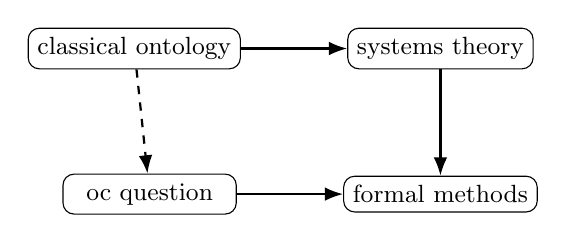
\begin{tikzpicture}[node distance=1.35cm,>=Latex,every node/.style={font=\small}]
\node[draw,rounded corners,align=center,minimum width=2.2cm] (a) {classical ontology};
\node[draw,rounded corners,align=center,minimum width=2.2cm,right=of a] (b) {systems theory};
\node[draw,rounded corners,align=center,minimum width=2.2cm,below=of b] (c) {formal methods};
\node[draw,rounded corners,align=center,minimum width=2.2cm,left=of c] (d) {oc question};
\draw[->,thick] (a) -- (b);
\draw[->,thick] (b) -- (c);
\draw[->,thick] (d) -- (c);
\draw[->,thick,dashed] (a) -- (d);
\end{tikzpicture}
\caption{Ontology of Continua Attempts: dependency dag of historical sequence pressure 8-1-3}
\label{fig:figure-what-the-ontology-of-continua-attempts-to-do-one}
\end{figure}
The point of the diagram is not decoration; it marks which relation is being proposed and which stronger conclusion is still unavailable.\par
A local clarification is useful here\par
A local clarification is useful here\footnote{In Ontology of Continua Attempts, this note clarifies the reader clarification role of the term and keeps the caveat close to the sentence that needs it.}.\par
The note keeps the caveat near the term without derailing the main sentence.\par
Consider a lake receiving nutrient runoff from nearby farms. For a time, the added nutrients enter an ecology that still absorbs them as variation. Algae increase in some seasons. Fish populations shift. Dissolved oxygen rises and falls with temperature, depth, plant life, and decay. The shoreline remains inhabited by familiar species. The lake is changing, but the questions asked of it still belong to the same organization: how much nutrient input can be tolerated, how seasonal blooms behave, how fish and plants adjust, how oxygen moves through the water column.\par
Then the same lake may enter another condition. Algal blooms thicken and persist. Light no longer reaches the same depths. Plant communities alter. Dead organic matter increases decomposition demand. Oxygen falls in deeper water. Fish kills become more likely. The water remains water, the basin remains the basin, and the map still names the same lake. But the organization that made earlier descriptions adequate has weakened or failed. The point is not simply that one measured value has become large. The relations among nutrients, algae, oxygen, decomposition, light, species survival, and intervention have changed their pattern. The lake has become harder to describe as a clear-water system under seasonal stress and easier to describe as a eutrophic system organized around reinforcing degradation.\par
This is the kind of passage that interests OC. It is not a separate ecology of lakes. It does not decide the sampling design, establish the causal model, or replace field measurements. Its concern is the descriptive difference between movement within an organization and transformation of that organization. The same nutrient input that once counted as variation can later become part of a process that moves the lake toward another regime. The same boundary that once seemed physical, the shoreline or basin, proves insufficient. A more important boundary may lie in the organization of the ecology itself: the range within which the lake can absorb disturbance and still remain intelligible under the previous description.\par
Once this is seen, several terms become necessary, not as ornaments but as handles for the problem. The lake is treated as a system when its relations are bounded for analysis: water, species, nutrient inflow, oxygen dynamics, sediments, weather, and human intervention are not the whole universe, but they are the configuration under consideration. Nutrient loading, oxygen concentration, algal biomass, water clarity, and species composition are not interchangeable, yet each can form an ordered direction of relevant variation. OC calls such a direction a continuum when movement along it matters to the organization being described. The limit at which a movement ceases to be ordinary variation and begins to alter the description functions as a boundary. A change imposed or considered, such as increased runoff, reduced inflow, aeration, dredging, or regulation, functions as an operator when it transforms the described condition of the system.\par
These words are deliberately modest. They do not make the lake abstract in order to make it easier. They slow the description down. They ask what is changing, along which ordered fields of variation, under which boundaries, through which transformations, and with what consequence for the organization that made the original description meaningful. OC begins there: with the wish to compare changing systems without dissolving their differences.\par
\section{What the Tradition Made Visible In Ontology of Continua Attempts}
The problem matters because thought often fails in two opposite ways. One failure comes from excessive separation. Each domain becomes so local that no comparison can survive beyond metaphor. Chemistry speaks only to chemistry, ecology only to ecology, software only to software, political theory only to political theory. The other failure comes from excessive unity. A general vocabulary expands so quickly that it ceases to respect the measurements, constraints, and objects of the fields it touches. OC attempts a more difficult middle position. It seeks comparison across domains while preserving the authority of local evidence. \cite{haken_synergetics,nicolis_prigogine_selforg}\par
This ambition has neighbors. The study of self-organization, nonlinear dynamics, synergetics, nonequilibrium systems, autocatalytic networks, cybernetics, and complexity has already shown that order, instability, feedback, and regime change are not marginal curiosities. They are central to how organized systems are described. Hermann Haken's work on synergetics gave one influential account of how macroscopic patterns can arise from interacting microscopic components. Ilya Prigogine and Isabelle Stengers, along with the broader nonequilibrium tradition, helped make instability and dissipative organization philosophically and scientifically visible. Stuart Kauffman's work on autocatalytic sets, and later formal studies of reflexively autocatalytic and food-generated networks, made self-sustaining organization precise in settings where components help produce the conditions for their own persistence.\par
The local dependency can now be written without changing the claim it supports.\par
\begin{equation}\label{eq:equation-what-the-ontology-of-continua-attempts-to-do-two}
\operatorname{claimSupport}_{1} = \rho_{\mathrm{replay}}=\frac{N_{\mathrm{matched}}}{N_{\mathrm{declared}}}
\end{equation}
The relation names a local dependency, variable dictionary, and proof/evidence role; it is not a claim-status upgrade.\par
The formula is a restraint on the prose. It names the dependency that the surrounding paragraph is allowed to use.\par
The comparison below gives ontology of continua attempts a set of quantities that can be inspected instead of merely admired.\par
\begin{table}[htbp]
\centering\small
\caption{Ontology of Continua Attempts: observable quantities and counter-pressure 8-2-3}
\label{tab:table-what-the-ontology-of-continua-attempts-to-do-one}
\begin{tabular}{@{}llll@{}}
\toprule
Model & Retained insight & Rejected assumption & OC extension \\
\midrule
ontology of continua attempts boundary & 18 units & declared case & fixes what is compared \\
residual pressure & 0.42 & dimensionless & shows unresolved load \\
projection loss & 0.66 & bounded interval & marks lost structure \\
countercase set & 11 cases & review sample & keeps a falsifier visible \\
\bottomrule
\end{tabular}
\end{table}
The table should be read locally: it narrows the comparison without pretending that the wider theory has been settled by a single surface.\par
OC does not absorb these traditions or claim priority over them. It approaches a different layer of the problem. It asks how descriptions of organized change can be compared when the things compared are not made of the same stuff, measured in the same units, or governed by the same models. A lake, a reaction network, a software platform, and an institution cannot be made identical without intellectual damage. But each can force the same kind of descriptive question: when does a system vary within a current organization, and when does the organization of description itself have to change?\par
The lake makes this question concrete. Nutrient concentration is measurable. Dissolved oxygen is measurable. Fish mortality can be observed. Algal density can be estimated. But the claim that the lake has shifted regime is not identical with any one measurement alone. It depends on relations among measurements, on persistence over time, on feedback among processes, and on the interpretive boundary between ordinary ecological variation and altered organization. OC gives language for that relational level while leaving the measurement to the relevant sciences.\par
The same need appears in artificial systems, though the materials are different. Imagine an online service made of several dependent components: an authentication service, a database, a cache, a payment service, a message queue, and a public interface. At low and moderate load, traffic fluctuates inside expected limits. The cache absorbs repeated requests. The queue smooths bursts. The database slows but recovers. Engineers can describe the system as stressed but functioning. The relevant questions concern capacity, latency, retry rates, and resource allocation within a known architecture.\par
Now suppose a promotional event drives traffic far beyond ordinary expectations. The authentication service slows. Clients retry. Those retries add load. The queue fills. Timeouts cause upstream services to resend requests. The database begins to lock under competing writes. Monitoring dashboards show errors, but the first visible symptom is not the whole cause. Each service behaves according to rules that made sense in ordinary conditions: retry failed requests, preserve consistency, wait for authentication, protect data, keep accepting traffic. Together those rules now amplify the failure. The platform has not merely become slower. Its organization under load has changed. Measures designed for resilience have become part of the cascade.\par
Here OC helps distinguish a simple overload from a collapse of operating organization. In a simple overload, adding capacity or reducing traffic may restore the same pattern. In a cascade, local recovery procedures can deepen the failure because the relations among services have become the main problem. The system's boundary is not just the list of machines. It includes dependency relations, retry policies, timeout settings, queue limits, observability assumptions, and human response procedures. The operator is not merely traffic growth. It may be the combination of traffic growth with automatic retries, strict consistency requirements, and delayed circuit breaking. The contradiction is not that engineers want high availability and low cost. That is a tradeoff. The sharper incompatibility appears when the organization requires every service to preserve its local rule while the joint operation of those rules prevents the platform from remaining available.\par
This software case is not physically identical to the lake. Algae are not retries. Oxygen is not latency. Fish mortality is not database lock contention. A valid comparison does not equate the objects. It compares forms of organization: reinforcing processes, boundary stress, local rules that become globally destructive, and a shift from ordinary variation to altered regime. An invalid comparison would say that because both systems collapse, the same intervention must work in both. Aeration belongs to one domain; circuit breakers belong to another. OC permits the structural comparison while forbidding the transfer of local remedies without domain evidence.\par
That distinction is central. A common language is valuable only if it does not smuggle false sameness into the analysis. The lake teaches one lesson about reinforcing degradation; the software platform teaches another about dependency, retry, and cascade. Their comparison becomes useful when it sharpens attention to organization. It becomes irresponsible when it ignores material difference. OC attempts to hold both facts at once.\par
\section{Where the Inheritance Runs Out In Ontology of Continua Attempts}
The central hypothesis of OC is easiest to state after the examples have done some work: when a configuration contains an unresolved contradiction, that contradiction tends either to require a new dimension of description or to contribute to collapse of the configuration that cannot resolve it. This is not a validated causal law across all domains. It is a comparative descriptive proposal. Its purpose is to organize inquiry into cases of organized change, not to decide those cases in advance. \cite{haken_synergetics,nicolis_prigogine_selforg}\par
The word contradiction is important and easily misused. OC does not mean any conflict, inconvenience, pressure, or tradeoff. A company that wants lower cost and higher quality does not thereby contain a contradiction. A lake that receives nutrients and loses oxygen does not automatically contain one either. A contradiction, in this usage, is a structured incompatibility inside a defined organization: two or more active conditions are required by the organization, yet cannot be jointly sustained under that organization as it stands.\par
The local dependency can now be written without changing the claim it supports.\par
\begin{equation}\label{eq:equation-what-the-ontology-of-continua-attempts-to-do-one}
\operatorname{domainError}_{1} = G=(V_{\mathrm{claim}}\cup V_{\mathrm{evidence}},E_{\mathrm{support}}\cup E_{\mathrm{challenge}})
\end{equation}
The relation names a local dependency, variable dictionary, and proof/evidence role; it is not a claim-status upgrade.\par
The formula is a restraint on the prose. It names the dependency that the surrounding paragraph is allowed to use.\par
The local dependency can now be written without changing the claim it supports.\par
\begin{equation}\label{eq:equation-what-the-ontology-of-continua-attempts-to-do-three}
\operatorname{levelClosure}_{1} = \epsilon_{\mathrm{domain}}=\max_i |y_i-\hat y_i|
\end{equation}
The relation names a local dependency, variable dictionary, and proof/evidence role; it is not a claim-status upgrade.\par
The formula is a restraint on the prose. It names the dependency that the surrounding paragraph is allowed to use.\par
A small numerical test keeps the abstraction honest at the scale of a single decision.\par
\paragraph{Numerical example.} For ontology of continua attempts, take support=0.57, projection loss=0., and 6 open obligations. The bounded score is 0.; the example gives the reader a numeric scale without pretending to be empirical proof.\par
The numbers are deliberately small; their value is pedagogical, not evidential, unless the chapter binds them to a dataset elsewhere.\par
In the lake, the contradiction becomes concrete only when the organization is specified. A clear-water lake under a certain ecological description requires enough light penetration, oxygen availability, plant balance, and species viability to preserve that regime. A pattern of nutrient inflow, algal growth, decomposition, and oxygen depletion may simultaneously require the lake to remain within that regime and drive it beyond the conditions that sustain it. The incompatibility is not a moral opposition between purity and pollution. It is a failure of joint satisfiability: the earlier organization requires conditions that the active processes increasingly destroy.\par
In the software platform, the contradiction can be stated with similar care. The architecture requires local services to follow rules meant to preserve correctness and availability: retry when a request fails, wait for authentication, write consistently, keep user sessions alive, and process queued work. Under cascading load, those rules become jointly unsustainable. The platform requires each local behavior to continue in order to preserve the service, while the combination of those behaviors prevents the service from remaining available. The contradiction is not simply high traffic. It lies in the incompatibility between the architecture's local obligations and its global condition of survival.\par
Two outcomes then become visible. Sometimes the contradiction opens a new dimension of description. Engineers may stop describing the platform only through average latency and server utilization and begin describing it through retry amplification, dependency depth, queue saturation, and failure propagation. Ecologists may stop describing the lake only through seasonal fluctuation and begin describing it through regime state, feedback strength, oxygen debt, and recovery threshold. The system has not necessarily become mysterious. It has demanded a richer axis of description.\par
At other times, no adequate reorganization occurs. The lake loses the living structure that supported its previous ecology. The software platform remains unavailable until traffic is cut, dependencies are isolated, or components are rebuilt. Collapse, in OC, names this loss of sustaining organization. It is not a theatrical word for bad news. A decline in a metric is not yet collapse. A temporary outage is not always collapse. Collapse appears when the organization that allowed the system to function as that kind of system can no longer sustain the conditions it requires.\par
Emergence is equally restrained. It does not mean novelty as such. A surprising bloom, a clever patch, or a new slogan is not automatically emergence. Emergence appears when a new descriptive dimension becomes necessary to understand the organization of the case. In the lake, the eutrophic regime may require variables and relations that were secondary in the clear-water description. In the software platform, failure propagation may become the central object, not a peripheral symptom. The new dimension is not invented for drama; it is forced by the inadequacy of the earlier description.\par
This is why a continuum in OC is neither a decorative metaphor nor necessarily a smooth mathematical line. It is an ordered field of variation relevant to the system under consideration. Nutrient loading can be such a continuum. So can oxygen availability, latency, dependency depth, legitimacy, centralization, or operational capacity, provided the axis is stated and disciplined by the domain. Some continua are measured with instruments. Some are constructed through institutional analysis. Some are formal. OC does not give them equal precision. It gives them a comparable role in description.\par
A boundary is likewise more than an edge. The shoreline is a physical boundary of the lake, but the boundary between ordinary seasonal variation and regime shift is organizational. The edge of a server cluster is a technical boundary, but the boundary that matters in a cascade may be the point at which retry behavior stops absorbing failure and starts multiplying it. Institutions have legal boundaries, procedural boundaries, symbolic boundaries, and practical boundaries. A parliament may survive disagreement within procedural rules, yet cross another boundary when factions cease to accept the procedures as binding. The boundary that matters is the condition under which a description remains valid.\par
An operator is any specified transformation considered within the analysis. In the lake, increased fertilizer runoff, wetland restoration, aeration, dredging, or nutrient regulation may function as operators. In the software platform, a traffic spike, a retry policy, a circuit breaker, a schema migration, a load balancer rule, or a manual shutdown may do so. The point is not to call every cause an operator. The point is to state what transformation is being applied to what description. Without that discipline, talk of change becomes too vague to inspect.\par
The hierarchy of continua enters when systems require more than one level of description. A molecule, a cell, an organism, a population, and an ecosystem are not simply different sizes of one object. Each level has its own relevant variation and its own boundaries. Lower-level processes constrain higher-level organization, while higher-level organization may stabilize or suppress lower-level variation. In software, machine resource limits constrain application behavior, while application architecture determines how those limits are encountered. In institutions, individual decisions matter, but procedural structures shape which decisions become consequential. OC uses hierarchy only in this restricted sense: levels of organized description must be named, and the relations among them must be shown.\par
The result is an operational metaontology. The phrase sounds abstract, but its purpose is practical. Ontology asks what kinds of things are being spoken of. Metaontology asks how such commitments are made and compared. Operational means that the vocabulary must help the analysis do something: identify the system, state the continua, mark the boundaries, specify the operators, describe the contradiction, and distinguish ordinary variation from emergence or collapse. If the vocabulary does not improve those tasks, it has no special right to remain.\par
\section{The Conceptual Debt In Ontology of Continua Attempts}
The vocabulary can now be gathered without turning the chapter into a glossary. A system is a bounded configuration of relations considered for analysis. The boundary may be physical, functional, formal, institutional, ecological, or conceptual, but it must be stated because different boundaries produce different claims. A lake bounded by shoreline, watershed, nutrient economy, or regional policy is not the same object for analysis, even if the same body of water is involved. \cite{haken_synergetics,nicolis_prigogine_selforg}\par
A continuum is an ordered field of possible variation relevant to that system. It need not be continuous in the strict mathematical sense. It may include thresholds, discrete states, categorical transitions, and discontinuities. What matters is that movement along the field can be ordered and that the ordering matters for the system. Nutrient loading, oxygen concentration, and algal density are obvious ecological examples. Retry amplification, latency, and dependency depth may serve in the software case. Legitimacy or procedural trust may serve in institutional analysis only if the construction is made explicit and tied to evidence.\par
A small numerical test keeps the abstraction honest at the scale of a single decision.\par
\paragraph{Numerical example.} For ontology of continua attempts, take support=0.60, projection loss=0.12, and 1 open obligations. The bounded score is 0.240; the example gives the reader a numeric scale without pretending to be empirical proof.\par
The numbers are deliberately small; their value is pedagogical, not evidential, unless the chapter binds them to a dataset elsewhere.\par
The case that follows turns the proposal into a sequence of criticizable moves.\par
\paragraph{Worked case.} In the worked case for ontology of continua attempts, the claim is reduced to a boundary, an observable, a dependency, a numerical cue, and a falsifier. The case is useful only because each move can be criticized separately.\par
The case helps because each step can fail separately, which is exactly what a useful example should permit.\par
A state is a placement, range, or condition within one or more continua. The term should not imply stillness. A lake in seasonal balance is not motionless; it is organized within ranges of movement. A software platform under normal traffic is not static; it is processing, failing locally, recovering, and adjusting. A state in OC is a way of locating the system within the relevant fields of variation, not a denial that processes continue.\par
A boundary marks the conditions under which a description holds. Some boundaries separate system from environment. Others separate one organization from another. In the lake, the watershed may be more analytically important than the shoreline if nutrient inflow is the question. In the software platform, the visible application boundary may matter less than the dependency graph through which failure propagates. In an institution, the formal constitution may matter less in a crisis than the practical boundary between accepted and rejected procedure. Boundaries become dangerous when they move silently, because a claim made under one boundary can be falsely carried into another.\par
An operator is a specified transformation of the system description. It may be causal, procedural, formal, experimental, or mathematical, depending on the domain. Adding nutrient input is an operator when the lake is analyzed under nutrient stress. Introducing a circuit breaker is an operator when the platform is analyzed under cascading failure. Dissolving a parliament, changing voting rules, or altering budget authority may be operators in institutional analysis. The discipline is simple: the analysis must say what is transformed, under what description, and with what expected or observed effect.\par
A contradiction is a structured incompatibility that cannot be resolved within the current organization without changing that organization, abandoning one of its active demands, or losing coherence. This narrow use prevents the term from becoming a synonym for tension. In the software case, it is not enough to say that reliability and cost conflict. A contradiction appears when the architecture requires local retry behavior to preserve service while the same behavior, under load, prevents service from being preserved. In the lake, it appears when the conditions of the prior ecological organization are required for persistence while active processes destroy those very conditions.\par
Projection is the practice of carrying a descriptive relation from one setting to another under stated limits. The lake and the software platform can be projected onto one another only at the level of organization: reinforcing processes, boundary stress, local dynamics that become globally destabilizing, and transition from ordinary variation to altered regime. That projection is valid only because it does not claim identity of substance, measurement, or remedy. The ecological evidence remains ecological. The engineering evidence remains engineering.\par
The invalid projection is just as important. It would be wrong to argue that because a lake can sometimes be restored by reducing nutrient input, a software cascade can be solved by reducing one numerical input alone. It would be equally wrong to claim that because circuit breakers isolate software failure, institutional crises can be solved by installing an equivalent procedural device without historical analysis. Projection does not license borrowed solutions. It licenses disciplined comparison of form under constraint.\par
The hierarchy of continua helps explain why projection must be careful. Each level of a system has its own relevant continua. A lake can be described through chemical concentrations, biological populations, hydrological flow, land-use policy, and regional climate. These are related, but not reducible to one another in ordinary analysis. A software platform can be described through CPU load, database locks, service dependencies, user behavior, deployment practice, and organizational response. A change at one level may alter another, but the path must be shown. OC is suspicious of leaps that skip levels because they often smuggle metaphor into places where evidence is needed.\par
The same caution applies to institutions. A political body may absorb disagreement for many years because procedures convert conflict into recognized decisions. The relevant continua might include procedural trust, administrative capacity, elite fragmentation, public legitimacy, and coercive dependence. These are not measured like oxygen concentration. They require historical and interpretive discipline. OC can help ask when disagreement remains ordinary variation and when procedural distrust becomes self-reinforcing. It cannot make the evidence easier than it is.\par
The vocabulary therefore has a double function. It makes comparison possible, and it makes exaggeration more visible. A proposed analysis must be able to say what the system is, which continua are relevant, where boundaries are drawn, what operators are active, what contradiction is claimed, and what would count as ordinary variation, emergence, collapse, or rejection of the claim. When those elements cannot be stated, the language has not earned its use. When they can be stated, the analysis becomes more inspectable even before it becomes formal.\par
\section{The Passage to Continua In Ontology of Continua Attempts}
A serious objection remains: perhaps OC is only a new arrangement of old ideas. Systems theory, cybernetics, nonlinear dynamics, synergetics, complexity theory, philosophy of science, ecology, computer science, and institutional theory already possess vocabularies for feedback, boundary, emergence, instability, and organization. OC cannot justify itself by acting as though those vocabularies do not exist. Its value, if it has one, lies in the particular work it asks its terms to perform: comparative description without premature unification. \cite{haken_synergetics,nicolis_prigogine_selforg}\par
The distinction is modest but important. A domain theory explains within its domain by using the objects, measurements, and methods proper to that domain. Limnology can investigate eutrophication in ways OC cannot. Distributed systems engineering can diagnose cascading failure in ways OC cannot. Political history can reconstruct institutional breakdown in ways OC cannot. OC does not compete with those inquiries. It asks how their descriptions of organized change may be placed beside one another without pretending that their evidence is the same.\par
This restraint is especially important for the central hypothesis. The claim about unresolved contradiction, new descriptive dimension, and collapse should never float above cases as a slogan. In some domains, contradiction can be formal and sharply stated. In others, it is operational or institutional and depends on interpretive evidence. The hypothesis has different strength in different settings. It may organize the question before it can settle the answer. That is acceptable only if the difference between organizing and proving remains clear.\par
The lake again keeps the limit visible. If field observations show rising nutrient input, persistent algal bloom, oxygen depletion, species loss, and resistance to recovery, OC may describe a transition in organization. But it does not supply the measurements. It does not determine sampling frequency. It does not replace hydrological modeling or ecological causation. It cannot certify that one intervention caused recovery unless the domain evidence supports that claim. OC can say what kind of change is being claimed. It cannot make the claim true by naming it.\par
The software case has the same constraint. A cascade may look obvious in retrospect, but engineering diagnosis must still establish dependency relations, timing, resource exhaustion, retry behavior, failure propagation, and recovery conditions. OC can help distinguish local error from system-level collapse. It can clarify the contradiction between local service obligations and global availability. It can mark the emergence of failure propagation as a new descriptive dimension. But it cannot replace logs, traces, architecture diagrams, incident review, or controlled remediation.\par
This discipline also protects the words emergence and collapse. Both terms are vulnerable to inflation. Emergence can become a name for anything interesting. Collapse can become a name for any loss. OC restricts them. Emergence requires the necessity of a new descriptive dimension. Collapse requires loss of sustaining organization. A stock price falling is not automatically collapse. A disagreement inside a government is not automatically institutional collapse. A new metric on a dashboard is not automatically emergence. The terms apply only when the system, continua, boundaries, operators, and contradiction have been made explicit enough to bear the weight.\par
Measurement raises a further difficulty. OC speaks across domains that do not share evidentiary standards. Chemical concentration, response latency, and institutional legitimacy are not the same kind of observable. A framework that treats them as interchangeable would be worse than useless. OC avoids that by locating comparison above local measurement, not in place of it. The framework may compare the role a variable plays in organized change, but it may not grant the variable more precision than the domain can justify.\par
There is also a philosophical danger. Any ontology can begin to mistake its categories for the world's furniture. OC tries to avoid that by treating its categories as commitments made for analysis. A system is not absolutely bounded for all purposes. It is bounded for the inquiry at hand. A continuum is not metaphysically ultimate. It is adopted because it captures relevant ordered variation. A boundary is not a wall in reality unless the domain makes it one. An operator is not a hidden force. It is a specified transformation in a specified description.\par
This approach leaves room for failure, and it must. Some projected comparisons will fail because the proposed mapping is too thin. Some continua will be badly chosen. Some alleged contradictions will dissolve once the system is described more carefully. Some supposed emergences will turn out to be ordinary variation under a better model. Some collapses will prove to be recoverable disturbances. These failures are not embarrassments external to the method. They are among the main reasons to have a disciplined vocabulary at all.\par
The affirmative project can now be stated plainly. OC tries to make organized change discussable at the level where systems differ in substance but resemble one another in form. It does not ask the reader to believe that lakes, software, institutions, organisms, and reaction networks are secretly the same. It asks whether certain questions can travel responsibly: What keeps this organization intelligible as itself? Along which ordered variations can it move? Where are its boundaries of interpretation? Which transformations act on it? What incompatibilities cannot be jointly sustained? When does a new dimension of description become necessary? When does the organization fail?\par
\section{A Problem Older Than the Vocabulary In Ontology of Continua Attempts attempts}
The opening task of OC is to make a particular kind of question askable. When a system changes, are we seeing movement within an existing description, a boundary crossing, the action of a transformation, the emergence of a new descriptive dimension, or the collapse of an organization that cannot sustain its own conditions? The question is broad, but it is not empty when each term is tied to a role that can be inspected. \cite{haken_synergetics,nicolis_prigogine_selforg}\par
The lake under nutrient stress remains useful because it resists pure abstraction. It has measurable variables, visible processes, reinforcing relations, possible thresholds, and real limits on interpretation. It shows why a continuum is not merely a line, why a boundary is not merely an edge, why an operator is not merely a cause, and why contradiction is not merely conflict. The software platform adds another lesson: a system can fail not because its parts abandon their rules, but because their rules become jointly destructive under changed conditions. Together the cases show how comparison can illuminate without erasing difference.\par
A reader can not leave this opening chapter thinking that the central hypothesis has been proved. It has only been made available for disciplined examination. The work ahead is to sharpen the vocabulary, formalize the relations, test projections, and show where the framework clarifies and where it must be narrowed. OC begins with vocabulary because later claims about organized change need terms that can survive public inspection. Its purpose is not to make every domain speak the same language. Its purpose is to let different domains be compared at the level of changing organization while their local evidence, methods, and constraints remain intact.\par
\chapter{How Different Readers Should Enter the Work}
\section{The Local Problem In Different Readers Should Enter}
OC Core 1.4 begins where many serious works of thought begin: not with a demand for belief, but with the problem of how belief, doubt, method, and comparison are to be kept in their proper places. The reader who opens this book may come from physics, philosophy, biology, computer science, mathematics, social theory, systems engineering, or no settled disciplinary home at all. Each arrival brings a different ear. One reader hears a claim about stability and asks where the variables are. Another hears a claim about being and asks what kind of thing has been named. Another hears talk of organization and asks whether purpose has been smuggled into a process that may require none. Another hears comparison across domains and asks what prevents metaphor from masquerading as science. These are not distractions from the work. They are part of the terrain the work must cross. \cite{nicolis_prigogine_selforg,kauffman_autocatalytic}\par
The book proposes an operational metaontology: a disciplined language for describing how systems are bounded, compared, transformed, and tested across domains. The phrase should be read slowly. Operational means that the vocabulary must show what it does. Metaontology means that the concern is not only with objects, but with the ways objects of inquiry are carved out, stabilized, related, and revised. The book is not claiming that a city, a cell, a proof, a software service, and a weather system secretly share one substance or one mechanism. It is claiming that descriptions of such things often face recurring difficulties: where to draw a boundary, how to follow change without losing identity, how to compare one domain with another, how to recognize a conflict that a current description cannot resolve, and how to keep explanatory reach within the limits of what has actually been shown.\par
The next diagram slows the argument down just enough to show how different readers should enter is being organized.\par
\begin{figure}[htbp]
\centering
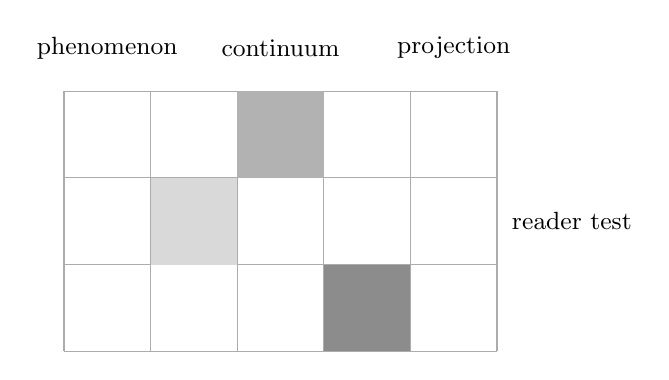
\begin{tikzpicture}[node distance=1.35cm,>=Latex,every node/.style={font=\small}]
\draw[step=1.1cm,gray!65,thin] (0,0) grid (5.5,3.3);
\node[align=center] at (0.55,3.85) {phenomenon};
\node[align=center] at (2.75,3.85) {continuum};
\node[align=center] at (4.95,3.85) {projection};
\node[align=center] at (6.45,1.65) {reader test};
\fill[black!15] (1.1,1.1) rectangle (2.2,2.2);
\fill[black!30] (2.2,2.2) rectangle (3.3,3.3);
\fill[black!45] (3.3,0) rectangle (4.4,1.1);
\end{tikzpicture}
\caption{Different Readers Should Enter: evidence matrix of conceptual dependency pressure 9-1-4}
\label{fig:figure-how-different-readers-should-enter-the-work-one}
\end{figure}
The point of the diagram is not decoration; it marks which relation is being proposed and which stronger conclusion is still unavailable.\par
A local clarification is useful here\par
A local clarification is useful here\footnote{In Different Readers Should Enter, this note clarifies the reader clarification role of the term and keeps the caveat close to the sentence that needs it.}.\par
The note keeps the caveat near the term without derailing the main sentence.\par
The opening task, then, is delicate. A reader needs a way into the vocabulary without being asked to accept too much too soon. A language can be useful before it is complete, but only if its use is kept honest. OC does not ask the reader to treat its first definitions as conclusions. It asks the reader to notice what becomes clearer when the same care is applied to systems, boundaries, continua, operations, contradictions, emergence, and collapse. To enter the work well is not to join a school. It is to learn how the book separates a term from a claim, a comparison from a proof, an example from a dataset, and a formal possibility from an established result.\par
This matters because the strongest objections to a general vocabulary are also the objections that can make such a vocabulary worth building. If the language is too loose, it will merely rename familiar things. If it is too rigid, it will fail whenever it leaves the domain in which it was born. If it travels without discipline, it will inflate analogy. If it refuses to travel at all, it will miss structures that recur across fields in different materials. The work therefore begins by making the act of reading itself part of the discipline. Not because readers are to be sorted into fixed types, but because different questions have different standards, and a serious theory must not let those standards blur.\par
\section{The Necessary Distinction In Different Readers Should Enter}
Scientific languages often travel faster than their warrant. A term born inside one research program becomes attractive elsewhere because it appears to organize a difficult case. Self-organization, emergence, criticality, network, attractor, hierarchy, collapse, adaptation, and resilience have all lived this double life. They name real work, often precise and demanding work, yet they also invite overextension. Nicolis and Prigogine gave self-organization a thermodynamic and dynamical setting. Kauffman gave autocatalytic order a biological and combinatorial setting. RAF network theory later sharpened one part of that discussion by specifying reflexively autocatalytic food-generated networks. Bak's work on self-organized criticality made scale, instability, and avalanche-like behavior central to a different class of systems. These lineages should not be flattened into a common slogan. \cite{nicolis_prigogine_selforg,kauffman_autocatalytic}\par
OC enters this landscape with restraint. It does not replace those literatures, and it does not claim that a social institution, a chemical network, a mathematical proof, and a living cell share the same observables. Its wager is narrower and more architectural: whenever a system is described as organized, bounded, changing, contradictory, emergent, or collapsing, the description should say what has been held fixed, what has been allowed to vary, what operation has been performed, and what kind of comparison is being attempted. Without that discipline, one field's useful term may become another field's ornament.\par
The local dependency can now be written without changing the claim it supports.\par
\begin{equation}\label{eq:equation-how-different-readers-should-enter-the-work-two}
\operatorname{simulationDrift}_{1} = \kappa_{K_1}=\frac{b_{K_1}+s_{K_1}}{1+o_{K_1}+q_{K_1}}
\end{equation}
The relation names a local dependency, variable dictionary, and proof/evidence role; it is not a claim-status upgrade.\par
The formula is a restraint on the prose. It names the dependency that the surrounding paragraph is allowed to use.\par
The comparison below gives different readers should enter a set of quantities that can be inspected instead of merely admired.\par
\begin{table}[htbp]
\centering\small
\caption{Different Readers Should Enter: observable quantities and counter-pressure 9-2-4}
\label{tab:table-how-different-readers-should-enter-the-work-one}
\begin{tabular}{@{}llll@{}}
\toprule
Input & Operation & Output & Open condition \\
\midrule
different readers should enter boundary & 21 units & declared case & fixes what is compared \\
residual pressure & 0.49 & dimensionless & shows unresolved load \\
projection loss & 0.77 & bounded interval & marks lost structure \\
countercase set & 12 cases & review sample & keeps a falsifier visible \\
\bottomrule
\end{tabular}
\end{table}
The table should be read locally: it narrows the comparison without pretending that the wider theory has been settled by a single surface.\par
Consider a coastal city responding to repeated flooding. The city can be described physically, as land, water, infrastructure, elevation, drainage, and energy flow. It can be described administratively, as agencies, budgets, zoning rules, tax bases, emergency protocols, insurance maps, and legal responsibilities. It can be described socially, as households, memory, trust, risk tolerance, displacement, habit, and attachment to place. It can be described ecologically, as wetlands, sediment, salinity, species movement, storm absorption, and changed relations between built and living systems. A single flood crosses all these descriptions, but it does not mean the same thing in each one. Water in a street is a hydraulic event, an administrative failure or success, a household crisis, a financial signal, and an ecological interaction, depending on the domain in which it is being read.\par
If one demands a single master variable, the city becomes falsely simple. If one rejects comparison because no master variable exists, the city becomes falsely fragmented. OC tries to preserve another possibility. It asks how several continua of description may be named without being fused. A continuum, in this book, is a structured range along which a system can vary while still being treated as the same object of inquiry. In the coastal city, water level, evacuation readiness, insurance exposure, public trust, neighborhood displacement, and wetland absorption are not one continuum. They are different continua that may become coupled under stress. Their coupling matters because a change in one range may alter the meaning or viability of another.\par
The example is social, physical, ecological, and administrative at once, but the vocabulary is not tailored only to cities. A protein complex offers a different test. It may be described structurally, through folded shapes and binding sites; chemically, through affinities, charge distributions, and reaction conditions; dynamically, through conformational change; functionally, through the role it plays in a pathway; and experimentally, through the instruments that make it visible. Its boundary is not merely its outer surface. It may be drawn around a chain, a dimer, a transient complex, a catalytic site, or an interaction network. Its continua may include binding affinity, temperature sensitivity, conformational flexibility, concentration, and reaction rate. An operation may isolate the complex, mutate a residue, change the solvent condition, compare two states, or model a transition. A contradiction may appear when the same structure must remain stable enough to preserve function and flexible enough to perform it. Nothing in this comparison says that a protein is a city. The point is that disciplined description faces recognizable pressures in both cases.\par
The difference matters because later claims about contradiction, emergence, and collapse depend on it. If the book says that an unresolved contradiction may give rise to a new dimension of description or may collapse the configuration that cannot resolve it, the reader must already know what kind of configuration is being discussed and what counts as a dimension of description. Otherwise the sentence sounds large while doing little work. The vocabulary is meant to slow the claim down until it can be inspected. What is the system? Where is the boundary? Which continuum is changing? What operation made the change visible? What has failed, persisted, or been transformed?\par
\section{The Testable Step In Different Readers Should Enter}
The central concept needed at the threshold is the entry route. The phrase does not name a personality type, a disciplinary rank, or a preferred class of reader. It names the ordered way a question approaches the theory. A page may be read as motivation, as ontology, as formal vocabulary, as model proposal, as empirical claim, as philosophical speculation, or as preparation for later mathematical work. These readings can coexist, but they cannot be allowed to substitute for one another. A metaphor may motivate a model, but it is not a model. A model may sharpen a claim, but it is not yet evidence of the world. An example may clarify a term, but it is not a theorem. The entry route keeps the first question from silently becoming every question. \cite{nicolis_prigogine_selforg,kauffman_autocatalytic}\par
The coastal city shows why this restraint is necessary. A reader approaching through physical modeling may ask whether storm surge, drainage capacity, soil saturation, power failure, and road obstruction can be represented with measurable variables. That is a legitimate approach, and without it the city may be described with eloquence but little engineering force. Yet this approach cannot by itself settle questions of political legitimacy, household attachment, tax policy, or collective memory. A reader approaching through social theory may see that displacement changes the identity of the city even if the skyline remains. That, too, is legitimate. Yet it cannot determine the hydrodynamics of the next storm. The point is not to keep these readings apart forever. The point is to prevent their premature fusion.\par
The local dependency can now be written without changing the claim it supports.\par
\begin{equation}\label{eq:equation-how-different-readers-should-enter-the-work-one}
\operatorname{falsifierHit}_{1} = \operatorname{support}(c_{1})=P(c_{1})\wedge E(c_{1})\wedge R(c_{1})
\end{equation}
The relation names a local dependency, variable dictionary, and proof/evidence role; it is not a claim-status upgrade.\par
The formula is a restraint on the prose. It names the dependency that the surrounding paragraph is allowed to use.\par
The local dependency can now be written without changing the claim it supports.\par
\begin{equation}\label{eq:equation-how-different-readers-should-enter-the-work-three}
\operatorname{datasetSeparation}_{1} = \operatorname{falsify}(h)=\exists e\in E\,:\,\operatorname{pred}_h(e)\neq\operatorname{obs}(e)
\end{equation}
The relation names a local dependency, variable dictionary, and proof/evidence role; it is not a claim-status upgrade.\par
The formula is a restraint on the prose. It names the dependency that the surrounding paragraph is allowed to use.\par
A small numerical test keeps the abstraction honest at the scale of a single decision.\par
\paragraph{Numerical example.} For different readers should enter, take support=0.43, projection loss=0.17, and 2 open obligations. The bounded score is 0.; the example gives the reader a numeric scale without pretending to be empirical proof.\par
The numbers are deliberately small; their value is pedagogical, not evidential, unless the chapter binds them to a dataset elsewhere.\par
The same pattern appears in the protein complex. A structural biologist may ask what shape is occupied under specified conditions. A biochemist may ask which reaction is accelerated or inhibited. A systems biologist may ask how the complex participates in a pathway. A computational modeler may ask which states can be represented and which transitions are probable. A philosopher of science may ask whether the chosen boundary is a convenience of measurement or a claim about the object itself. These approaches do not cancel one another. They make different demands. The entry route gives each demand a place without allowing any one of them to pretend it has exhausted the object.\par
This is why the book begins with description before pressing toward formal claims. OC needs the reader to distinguish a domain from a projection. A domain is the field of inquiry in which observations, measurements, practices, and standards have their ordinary force. A projection is a disciplined rendering of one domain's structure into another descriptive language. Calling the city a legal municipality is a domain-specific description. Calling it an adaptive system is a projection. Calling it a coupled infrastructure-social-ecological configuration is a more complex projection, one that must still specify what is being coupled, under what boundary, and for what purpose. Calling a protein complex a machine may be useful in one setting and misleading in another, unless the operation behind the comparison is stated.\par
Emergence requires the same care, though the path into it is often obscured by the word's appeal. In ordinary speech, emergence can mean surprise, novelty, collective pattern, unexpected order, or simply ignorance of the details. In scientific use, it must be tied to a relation between lower-level interactions and higher-level regularities. OC uses emergence only after introducing the levels, the boundary, and the operation that connects them. An operation, in this book, is a rule-governed transformation or comparison performed on a described system. Drawing a boundary, projecting a domain, coupling two continua, identifying a contradiction, testing persistence under change, or comparing two configurations are all operations. The term operation matters because it turns vague movement into inspectable action.\par
A reader approaching through intellectual history will see familiar problems: form and change, unity and multiplicity, cause and constraint, persistence and transformation. A reader approaching through complex systems will notice kinship with self-organization, autocatalysis, criticality, attractors, thresholds, and cascades. A reader approaching through formalization will ask which terms can receive mathematical definition and which remain conceptual. A reader approaching through empirical science will ask what has been observed, simulated, compared, reproduced, or measured. A reader approaching through engineering will ask what the vocabulary helps one build, diagnose, or prevent. OC needs all of these approaches, but it cannot let any one of them become the whole building.\par
The discipline is especially important because the book will sometimes speak across domains. Cross-domain speech is not a license for sameness. It is a demand for cleaner distinctions. When OC compares a city and a protein complex, it is not claiming that residents are molecules or that institutions fold. It is asking whether the acts of bounding, tracking variation, naming operations, and locating structured incompatibility can be made explicit in both cases. If they can, then comparison becomes possible without identity. If they cannot, the comparison should fail. A useful vocabulary must be able to say no to its own extensions.\par
\section{An Objection Worth Keeping In Different Readers Should Enter}
Several terms must be fixed before later chapters can use them without confusion. A system is any object of inquiry treated as having enough persistence to be described across change. This does not mean the system is natural, closed, simple, or perfectly bounded. A thunderstorm, a protein complex, a court, a software service, a market, a mathematical proof, and a city can all be treated as systems only after the description states what is being tracked. The word system does not confer unity by itself. It marks a decision to examine something as organized enough for comparison across variation. \cite{nicolis_prigogine_selforg,kauffman_autocatalytic}\par
A boundary is the rule by which a description distinguishes what is inside the system from what is outside it. Boundaries are not always physical edges. The wall of a container is a physical boundary. A membership rule is an institutional boundary. A file format is a technical boundary. A species concept is a biological boundary. A budget line is an administrative boundary. The boundary of a proof may be drawn around axioms, permitted rules of inference, definitions, lemmas, or the completed argument. OC treats boundary placement as an operation because different placements change what can be claimed. The same material situation may yield different systems when the boundary changes.\par
A small numerical test keeps the abstraction honest at the scale of a single decision.\par
\paragraph{Numerical example.} For different readers should enter, take support=0.46, projection loss=0.10, and 3 open obligations. The bounded score is 0.; the example gives the reader a numeric scale without pretending to be empirical proof.\par
The numbers are deliberately small; their value is pedagogical, not evidential, unless the chapter binds them to a dataset elsewhere.\par
The case that follows turns the proposal into a sequence of criticizable moves.\par
\paragraph{Worked case.} In the worked case for different readers should enter, the claim is reduced to a boundary, an observable, a dependency, a numerical cue, and a falsifier. The case is useful only because each move can be criticized separately.\par
The case helps because each step can fail separately, which is exactly what a useful example should permit.\par
A continuum is a structured range of variation relevant to the system. Temperature across a chemical reactor, trust across an institution, abstraction across a proof, latency across a network service, binding affinity in a protein complex, and displacement pressure in a coastal city are different continua. They cannot be merged simply because each can be drawn as a line, assigned a number, or placed on a scale. A continuum is not just any difference. It is a range whose variation matters under the chosen description. To name a continuum is to say which kind of change can occur while the system remains recognizable enough to study.\par
An axis is a named direction within a continuum along which comparison is being made. In the coastal city, flood depth may be one axis within a physical-risk continuum, while evacuation compliance may be one axis within an administrative-behavioral continuum. In a protein complex, binding affinity may be one axis within a chemical-interaction continuum, while conformational flexibility may be one axis within a structural-dynamic continuum. The axis does not carry meaning by itself. Its meaning comes from the domain, the method of observation or measurement, and the boundary used to define the system. A number without its axis is mute; an axis without its domain is unstable.\par
An operation is a rule-governed act performed on a described system. It may be conceptual, mathematical, experimental, computational, administrative, or observational, depending on the domain. Drawing a boundary is an operation. Coupling two continua is an operation. Projecting one domain into another language is an operation. Mutating a residue in a protein, changing a zoning rule in a city, abstracting a lemma in a proof, or rerouting traffic in a software service may each be treated as an operation if the description states what is being transformed and what counts as a result. OC uses the term to make action explicit. A claim about change should say what changed, under which operation, and according to which standard.\par
A configuration is the current arrangement of relevant systems, boundaries, continua, and operations. The term is deliberately broader than mechanism. A mechanism explains how something occurs. A configuration names the organized situation in which several mechanisms, constraints, descriptions, and conflicts may interact. A coastal city before a storm, during a storm, after repeated rebuilding, or after managed retreat may occupy different configurations. A protein complex before binding, after binding, during catalysis, or after mutation may do the same. A configuration can persist, adapt, reveal a new descriptive need, or fail to maintain the relations that made it identifiable.\par
A contradiction, in OC usage, is not merely a logical inconsistency in prose. It is a structured incompatibility inside a configuration. The incompatibility may be formal, operational, institutional, ecological, biological, technical, or conceptual, depending on the domain. A city that requires permanent coastal occupation for its tax base while its risk model increasingly demands retreat contains a contradiction in this operational sense. A protein complex that must remain rigid to preserve a binding surface but flexible to complete its function may contain a different kind of contradiction, one that belongs to biochemical structure and dynamics rather than policy. The contradiction is not solved by naming it. It must be resolved, transformed, displaced, endured, or allowed to break the configuration.\par
The book's organizing hypothesis can now be stated with proper caution: in many configurations of the kind OC is built to examine, an unresolved contradiction tends either to force a new dimension of description or to collapse the configuration that cannot resolve it. This is not offered as an exhaustive law of all systems. It is a guiding hypothesis for the work that follows, a way of asking what happens when an existing description can no longer account for the incompatibility it has exposed. A new dimension of description appears when the old vocabulary cannot track what has become decisive. Collapse occurs when the configuration can no longer maintain the relations that made it identifiable under the chosen description.\par
In the coastal case, repeated flooding may force a shift from engineering defense alone to a combined description involving retreat, insurance withdrawal, ecological buffering, public legitimacy, and altered land use. The new dimension is not merely a new topic. It is a new range of relevance without which the system cannot be understood. In the protein case, a contradiction between stability and flexibility may force a description that includes conformational ensembles rather than a single static structure. What looked like one object under one representation may require a richer account of state, transition, and function. In both examples, the claim is not that the same mechanism is at work. The claim is that unresolved incompatibility can make the old descriptive frame insufficient.\par
No equation is required at this threshold because the present work is conceptual orientation. Later mathematical or formal surfaces must earn their own status. The vocabulary introduced here does not by itself prove that a given system will collapse, that a new dimension has appeared, or that one domain can be projected into another. It supplies terms through which such claims can become inspectable. If a later chapter offers a formal definition, that definition must carry its own burden. If it offers an empirical claim, the observations and methods must carry theirs. The present chapter prepares the language in which those burdens can be seen.\par
\section{The Result Of This Passage In Different Readers Should Enter}
A strong objection arrives almost immediately: if OC can describe cities, cells, proofs, networks, institutions, and software services, perhaps it is too general to be scientifically useful. A language that can speak about everything may risk explaining nothing. This objection should not be brushed aside. It is one reason the book separates vocabulary from evidence, projection from proof, and example from established result. Generality is not automatically a virtue. It becomes useful only when it improves discrimination. \cite{nicolis_prigogine_selforg,kauffman_autocatalytic}\par
The answer, therefore, cannot be that a broad language is valuable simply because it is broad. OC must help distinguish cases that looser language would blur. An autocatalytic chemical network and a city bureaucracy may both be called self-maintaining in ordinary language. But Kauffman's autocatalytic sets and RAF network theory give the chemical and prebiotic discussion particular structural requirements. A city agency maintaining its budget through annual appropriations is not thereby an autocatalytic set in the same scientific sense. OC may compare forms of persistence, dependence, closure, and reproduction, but it must not erase the difference between chemical organization and administrative renewal.\par
The danger is similar with self-organized criticality. Bak's account of systems reaching critical states has a specific scientific history and family of models. It cannot be converted into a universal metaphor for any crisis, cascade, or social breakdown. OC may ask whether a described configuration has thresholds, scale relations, accumulated stress, and cascading transitions. The answer depends on the domain and the evidence supplied. The word critical does not carry the claim. The discipline of the vocabulary lies in making such borrowed resonance answerable to the conditions under which it would be true.\par
Ontology raises another worry. A reader may suspect that OC multiplies entities: systems, boundaries, continua, axes, operations, configurations, contradictions, projections, dimensions. The worry is that acts of description have been turned into hidden furniture of the world. That is not the intended move. OC treats these terms operationally. They are not introduced as substances behind appearances. They are instruments for stating how a system is being described, compared, transformed, and challenged. The boundary is not always a thing in the world; sometimes it is a rule of attention. The continuum is not always a physical scale; sometimes it is an ordered range of institutional or conceptual variation. The operation is not always an experiment; sometimes it is a formal transformation or a disciplined comparison.\par
This does not make the terms arbitrary. A boundary drawn without consequence is decorative. A continuum named without a range of variation is empty. An operation with no rule is a gesture. A contradiction with no structured incompatibility is a mood. OC's vocabulary is meant to prevent precisely these failures. The terms are permissive enough to travel, but they must be specific enough to be refused. If a proposed boundary does no work, the description should say so. If a claimed contradiction is only a discomfort or a disagreement, it should not be treated as a contradiction in the stronger sense. If a projection imports a term from one domain into another without preserving any inspectable structure, the projection should be rejected.\par
Formalization imposes a further limit. Some readers will want a fully mathematical theory immediately. Others will prefer philosophical exposition and resist notation. OC cannot satisfy both by pretending that prose and proof have the same status. The present entrance fixes vocabulary and conceptual relations. Later formal work may define subsets of the vocabulary more strictly. A system may become a set with relations, a configuration may become a state in a structured space, an operation may become a mapping, a contradiction may become an incompatibility under constraints. But until such definitions are actually given in a particular case, the prose remains explanatory rather than demonstrative.\par
Evidence adds its own discipline. A living example can clarify a term, but it is not a dataset. A comparison can make a structure visible, but it is not a completed empirical test. A diagram can guide attention, but it is not a theorem. A simulation can explore a possibility, but it does not by itself establish that the same structure governs the world. The scientific value of OC depends on keeping these distinctions intact. Its early chapters prepare claims; they do not smuggle later validation into their own premises.\par
There is also a literary limit, though it is less often named in technical work. A language that is too ceremonious may make ordinary distinctions feel profound. A language that is too plain may fail to carry the complexity it needs to hold. OC must move between these risks. It needs enough abstraction to compare unlike domains, enough concreteness to prevent verbal inflation, enough caution to avoid false unity, and enough ambition to make the comparison worth attempting. A reader can expect the book to widen and narrow in turn: widening when it introduces a general operation, narrowing when it asks what the operation means in a specific domain.\par
The strongest protection against overreach is not modesty of tone alone. It is the repeated demand that every claim identify its level. Is this a definition, a proposal, a projection, a model, an observation, a formal result, or an interpretation? The same sentence may be harmless at one level and false at another. To say that a city and a protein complex both involve boundaries is a modest descriptive claim. To say that their boundaries work by the same mechanism would be a much stronger and usually false claim. To say that both can contain structured incompatibilities is a conceptual comparison. To say that the same law governs their failure would require a kind of support not yet supplied. OC's language exists so that these differences remain visible.\par
\section{The Local Problem In Different Readers Should Enter routesS0}
The book can be approached through several legitimate questions. One may ask where it belongs in the history of ideas about form, change, persistence, and contradiction. One may ask whether it clarifies problems already familiar in complex systems theory. One may ask which parts can be formalized and which parts remain conceptual. One may ask what kind of evidence could support its claims. One may ask whether the vocabulary helps in practical analysis of cities, organizations, biological systems, software services, proofs, or other structured objects of inquiry. None of these approaches is the master key. Each illuminates something and leaves something aside. \cite{nicolis_prigogine_selforg,kauffman_autocatalytic}\par
The key terms now in place are system, boundary, continuum, axis, operation, configuration, contradiction, projection, domain, emergence, collapse, and entry route. They are not decorative vocabulary. They are the minimum equipment needed to understand how OC tries to compare systems without flattening them into a single domain. A system is what the inquiry treats as persistent enough to track. A boundary states how that system is distinguished. A continuum names a structured range of variation. An axis gives direction within that range. An operation performs a disciplined transformation or comparison. A configuration gathers the relevant arrangement. A contradiction names a structured incompatibility within that arrangement.\par
The coastal city example shows why the equipment matters. A flood is physical, but not only physical. It is administrative, but not only administrative. It is ecological, but not only ecological. It is social, but not only social. When these descriptions become coupled, a contradiction may appear that the old description cannot resolve. A city may discover that the boundary that once made sense, the tax base, the shoreline, the evacuation zone, the protected district, no longer carries the same practical truth under repeated stress. The description may need a new dimension, or the configuration may fail to persist in its old form.\par
The protein example shows the same discipline under a different light. A complex is structural, but not only structural. It is chemical, but not only chemical. It is dynamic, but not only dynamic. It is functional, but not only functional. A static picture may be indispensable and still insufficient. A contradiction between stability and flexibility may force a richer description of states and transitions. Here again, OC does not claim that the biological case is the same as the civic one. It claims that the same descriptive questions can be asked without presuming the same answer.\par
The next movement can therefore begin the broader intellectual background without asking for premature belief. OC will stand or fall by the clarity of its definitions, the restraint of its projections, the quality of its formal work where formal work is claimed, and the adequacy of its evidence where evidence is claimed. This opening has one burden: to make the act of approach disciplined enough for later tests to matter. The reader need not accept the architecture in advance. It is enough, at first, to see why the architecture is needed, what distinctions it promises to preserve, and where its claims must still earn their force.\par
\chapter{What Counts as a Claim, Proof, Evidence, and Limit Here}
\section{From Claim To Obligation In Counts as Claim Proof}
A scientific claim is not the same thing as an interesting sentence. An interesting sentence may open a door, suggest a likeness, or give language to something half-seen. A scientific claim has a different burden. It must say what it is about, what its words mean in that setting, what kind of support it has, and what would make it weaker. This matters especially in a book that moves across biology, mathematics, social systems, cognition, and institutions. No single laboratory instrument waits behind all these subjects. No single kind of data can settle every question. The discipline has to come from the way the claims are made. \cite{kauffman_autocatalytic,raf_networks}\par
Consider a forest after decades of suppressed fire. Deadwood accumulates. Young growth fills spaces once cleared by smaller burns. Drought makes the vegetation less forgiving. A lightning strike that might once have passed through as local disturbance can now reorganize the whole landscape. One observer says, "The forest is unstable." Another says, "Fuel load has crossed a threshold." A third says, "A management policy has postponed small disturbances until the ecology must absorb a larger one." These sentences may all point toward the same scene, but they are not the same claim. Each one selects a different object, uses different words, requires different evidence, and fails in a different way.\par
The next diagram slows the argument down just enough to show how counts as claim proof is being organized.\par
\begin{figure}[htbp]
\centering
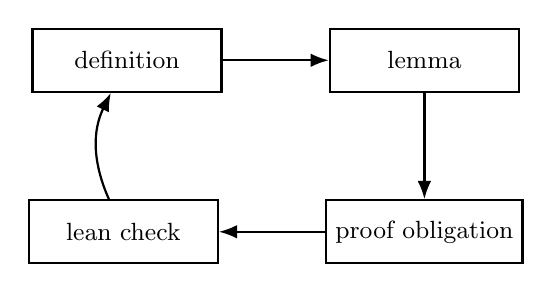
\begin{tikzpicture}[node distance=1.35cm,>=Latex,every node/.style={font=\small}]
\node[draw,thick,align=center,minimum width=2.4cm,minimum height=0.8cm] (a) {definition};
\node[draw,thick,align=center,minimum width=2.4cm,minimum height=0.8cm,right=of a] (b) {lemma};
\node[draw,thick,align=center,minimum width=2.4cm,minimum height=0.8cm,below=of b] (c) {proof obligation};
\node[draw,thick,align=center,minimum width=2.4cm,minimum height=0.8cm,left=of c] (d) {lean check};
\draw[->,thick] (a) -- (b);
\draw[->,thick] (b) -- (c);
\draw[->,thick] (c) -- (d);
\draw[->,thick,bend left=25] (d) to (a);
\end{tikzpicture}
\caption{Counts as Claim Proof: phase diagram of proof dependency pressure 10-1-5}
\label{fig:figure-what-counts-as-a-claim-proof-evidence-and-limit-here-one}
\end{figure}
The point of the diagram is not decoration; it marks which relation is being proposed and which stronger conclusion is still unavailable.\par
A local clarification is useful here\par
A local clarification is useful here\footnote{In Counts as Claim Proof, this note clarifies the reader clarification role of the term and keeps the caveat close to the sentence that needs it.}.\par
The note keeps the caveat near the term without derailing the main sentence.\par
The first task, then, is not to choose the grandest vocabulary. It is to notice what a sentence is asking the reader to accept. If we say that the forest is unstable, we need to know whether instability means frequent change, loss of resilience, increased probability of regime shift, or some other property. If we say fuel load has crossed a threshold, we need measurements, a model, or a history that gives that threshold meaning. If we say policy has displaced stress into the ecology, we have moved from a strictly ecological description into a description that includes human decision, institutional practice, and delayed consequence.\par
In this book, a claim is a bounded assertion about a system. A system is simply the organized object being described for the purpose at hand: a forest, a reaction network, a proof environment, a research institution, a market, a model, a concept, or a body. The word system does not mean that all such things are machines or that they are made of the same substance. It means that, for a given inquiry, their parts, relations, and changes are being considered together.\par
A claim becomes stronger when its commitments become easier to locate. The sentence "the forest is under stress" is a beginning. It becomes more serious when it names the forest, the period, the stressors, the relevant indicators, and the expected consequences. The same is true for a claim about a research institution. To say that an institution is under strain may be true but vague. To say that it rewards incompatible goals, suppresses methodological conflict, and loses trust in its own standards is a more inspectable claim. It may still be wrong, but one can now begin to examine it.\par
Proof has a narrower meaning. A proof is a formal or mathematical demonstration within stated assumptions. It can show that, given certain definitions and rules, a conclusion follows. It cannot by itself show that the world has arranged itself according to those definitions and rules. A proof inside a model is exact inside the model. Its reach beyond the model depends on further argument. This distinction is not a demotion of proof. It is what allows proof to retain its force.\par
Evidence is different from proof. Evidence includes observations, records, measurements, simulations, examples, comparisons, and empirical patterns that bear on a claim without becoming identical to demonstration. Fire histories, satellite records, field measurements, and ecological models may all serve as evidence for a claim about forest transition. They can corroborate, constrain, or weaken the claim. They may also be partial, noisy, local, or open to rival interpretation. Evidence matters because the world is not obliged to become transparent simply because a sentence is well formed.\par
A limit is a boundary on interpretation. Limits may come from missing data, narrow assumptions, idealized mathematics, untested domains, unresolved alternatives, or terms that are not yet measurable in a given setting. A limit is not decorative modesty. It is part of the knowledge being offered. If we know that a claim about one dry, fire-suppressed forest does not automatically apply to every forest, that limit protects the claim from becoming theatrical. It tells us where the sentence has earned its force and where it has not.\par
Some words used later in this book need to be introduced carefully because they do a great deal of work. A continuum is a dimension of variation along which something can change without becoming a wholly different object at every step. Temperature in a forest is an obvious example. Fuel density can also vary along a range. Institutional trust may vary too, although it is harder to measure and usually requires proxies. A continuum need not always be a perfectly numerical axis, but it must name some ordered difference that matters for the description.\par
An operator is a process, rule, action, or transformation that changes a system or its description. A drying season, a fire, a policy intervention, a catalytic reaction, a change in measurement scale, and a proof transformation may all function as operators in their own settings. The word does not make them identical. It asks what changes, under what constraints, and with what consequences. In the forest, drought acts differently from fire suppression, and both act differently from ignition. Calling them operators is useful only if those differences remain visible.\par
A boundary is a distinction that makes some differences count within a description while leaving others outside it. The edge of a forest may be a geographic boundary. The distinction between surface fire and crown fire may be a functional boundary. A research field may have boundaries formed by journals, methods, training, funding, or shared standards of evidence. Boundaries are not always walls. Often they are rules of relevance.\par
These three words, continuum, operator, and boundary, prepare the way for a fourth: contradiction. Contradiction here does not mean any disagreement, tension, or inconvenience. It means a structured conflict in which two requirements cannot be jointly satisfied under the present arrangement. A forest management regime may aim to prevent fire while producing the fuel conditions for more destructive fire. A research institution may reward novelty while punishing the methodological risk that genuine novelty requires. In such cases, the system is not merely experiencing pressure. It is preserving itself in a way that intensifies what it cannot absorb.\par
Only after these pieces are in place can the central hypothesis be stated responsibly. The hypothesis is that unresolved contradiction tends toward one of two outcomes: either the system requires a new dimension of description in order to become intelligible, or the configuration that cannot resolve the contradiction breaks down. In the forest, a simple account of "more or less fire" may no longer be enough; one may need to describe fuel structure, climate pattern, management history, species composition, and disturbance regime together. In the research institution, a simple account of "better or worse work" may no longer be enough; one may need to describe incentives, authority, method, and legitimacy as interacting dimensions.\par
This hypothesis is not a universal law already proven by being named. It is an organizing proposal. It earns strength only when particular claims are bounded, supported, and exposed to failure. The danger in any cross-domain theory is false unity. A network in ecology, a network in economics, and a network in computation can all be drawn with nodes and links, but the drawing alone does not make them the same kind of thing. Modern network science, as developed by figures such as Mark Newman, gives powerful tools for describing structure across cases while also making clear that the meaning of nodes and edges depends on the domain.\par
The same caution applies to emergence and collapse. Stuart Kauffman's work on autocatalytic organization and later formal studies of reflexively autocatalytic, food-generated networks show how organization can arise from relations among components rather than from a single commanding center. Per Bak's work on self-organized criticality shows how some systems can approach states in which small events have large consequences. These neighboring bodies of work are valuable because they teach disciplined ways to think about order, transition, and scale. They do not give permission to treat every crisis, organism, institution, or idea as the same kind of system.\par
The forest will remain our running example because it makes the problem concrete. The chapter could begin with a graph, a theorem, or a philosophical abstraction, but a forest under accumulated stress shows why claim discipline matters before the vocabulary becomes elaborate. We can see the difference between a sentence that dramatizes danger and a sentence that tells us what to inspect. We can see why evidence matters, why limits matter, and why comparison across domains must be earned. A theory that cannot keep those differences clear will not become more scientific by becoming more ambitious.\par
\section{The Dependency Spine In Counts as Claim Proof}
The method of this book is operational rather than devotional. It does not ask the reader to accept an entire ontology in advance. It begins with terms only when those terms make something inspectable. A useful term changes what can be seen, compared, tested, or rejected. A decorative term merely raises the temperature of the prose. \cite{kauffman_autocatalytic,raf_networks}\par
Take boundary again. If boundary only means a vague edge, it adds little. In the forest, however, boundaries can be physical, ecological, administrative, and conceptual. A fire line may mark an intended physical boundary. A change from grassland to dense woodland may mark an ecological boundary. A jurisdiction may mark who is responsible for management. A model may draw a boundary around the variables it includes. These boundaries interact, but they are not identical. The usefulness of the word lies in keeping their roles comparable without making their substance the same.\par
The local dependency can now be written without changing the claim it supports.\par
\begin{equation}\label{eq:equation-what-counts-as-a-claim-proof-evidence-and-limit-here-two}
\operatorname{proofDependency}_{2} = C_{\mathrm{unres}}=\min_{\pi\in\Pi}\|B(x)-B(\pi x)\|
\end{equation}
The relation names a local dependency, variable dictionary, and proof/evidence role; it is not a claim-status upgrade.\par
The formula is a restraint on the prose. It names the dependency that the surrounding paragraph is allowed to use.\par
The comparison below gives counts as claim proof a set of quantities that can be inspected instead of merely admired.\par
\begin{table}[htbp]
\centering\small
\caption{Counts as Claim Proof: observable quantities and counter-pressure 10-2-5}
\label{tab:table-what-counts-as-a-claim-proof-evidence-and-limit-here-one}
\begin{tabular}{@{}llll@{}}
\toprule
Case step & Observable & Numerical cue & Caveat \\
\midrule
counts as claim proof boundary & 24 units & declared case & fixes what is compared \\
residual pressure & 0.56 & dimensionless & shows unresolved load \\
projection loss & 0. & bounded interval & marks lost structure \\
countercase set & 13 cases & review sample & keeps a falsifier visible \\
\bottomrule
\end{tabular}
\end{table}
The table should be read locally: it narrows the comparison without pretending that the wider theory has been settled by a single surface.\par
The same pattern holds in a research institution. A department boundary may decide who reviews a proposal. A methodological boundary may decide what counts as admissible evidence. A career boundary may decide who can take intellectual risks. A conceptual boundary may decide which questions can even be asked. If an institution begins to fail, the explanation may require more than one of these boundaries at once. The word boundary helps only if it preserves the specific work each boundary performs.\par
Continuum works in a similar way. In a forest, fuel moisture, canopy density, and temperature may vary along measurable ranges. In an institution, trust, methodological tolerance, and administrative rigidity may also vary, but usually not with the same precision. The difference matters. A continuum may be quantitative, ordinal, qualitative, or model-relative. Calling something a continuum does not magically make it measurable. It says that some ordered variation is relevant and that the form of that variation must be stated.\par
Operators are the changes that matter within those boundaries and along those continua. In the forest, a lightning strike, a drought, a logging pattern, a policy of fire suppression, or an invasive species can transform the conditions of the system. In an institution, a funding rule, a review procedure, a publication norm, or a leadership change may play a comparable role. Comparable does not mean equivalent. The forest has no grant committee. The institution has no canopy. The comparison becomes useful only when the operator is translated into the local materials of the case.\par
This is why explanation must be distinguished from projection. Explanation stays close to a case. It identifies mechanisms, evidence, assumptions, and alternatives. Projection carries a structure from one domain into another. Projection is not automatically illegitimate. Much scientific thinking advances when a form recognized in one place illuminates another. But projection becomes careless when it carries prestige without translation. A concept from chemistry may help us think about social coordination only after we ask what corresponds to reaction, catalysis, boundary, supply, and persistence in the new domain.\par
Autocatalytic organization is a useful example. In the broad idea associated with Kauffman, a collection of molecular species may collectively support reactions that sustain the larger set. Later RAF theory gives this family of ideas sharper formal expression by studying reaction systems that are both reflexively autocatalytic and food-generated. This work can illuminate a general possibility: order need not always descend from a central designer. Relations among parts can help produce and maintain the whole. But it would be a mistake to infer from this that every organized social, cognitive, or institutional system is autocatalytic in the same sense. The analogy has to be earned again in each setting.\par
The forest and the research institution show the same requirement. Both may accumulate stress. Both may resist small corrections until larger reorganization becomes more likely. Both may have boundaries that once stabilized the system and later trap it. Yet their evidence differs. For the forest, one might examine fire history, fuel load, climate data, species composition, and recovery after disturbance. For the institution, one might examine hiring patterns, review norms, citation practices, failed reforms, internal reports, and the distribution of authority. The shape of the comparison is meaningful only when the difference in evidence is respected.\par
Citations also belong inside this discipline. A reference to network science is not a badge that makes a sentence rigorous. It points to a body of work on how relational structures can be modeled and measured. A reference to self-organized criticality points to a family of models in which systems may approach critical states and produce event patterns that challenge simple linear expectation. A reference to autocatalytic organization points to research on how mutually supporting relations can sustain organized sets. None of these references makes the present framework true. They locate neighboring work that clarifies what may be borrowed and what must be proven separately.\par
A later formal passage may show that, under defined assumptions, a relation follows. That is proof in the formal sense. A later empirical passage may show that a particular domain exhibits a pattern compatible with the framework. That is evidence. A later comparison may show that one vocabulary preserves a distinction that another vocabulary blurs. That is comparative argument. These forms can cooperate, but they cannot replace one another.\par
The method is therefore simple in spirit, though demanding in practice. Compare systems, but do not smuggle identity into comparison. Use shared vocabulary, but do not let the vocabulary pretend that empirical work has already been done. Build formal structures, but do not let formal elegance drift into domain validation. Use examples, but do not ask them to carry more weight than examples can bear. A forest can teach us how to think about delayed disturbance. It cannot prove a theory of institutions. An institution can teach us how contradiction may be organized by norms and incentives. It cannot prove a theory of ecology.\par
This separation is what allows a broad inquiry to remain readable. A theorem, a field record, a simulation, a historical episode, and a conceptual distinction answer different questions. If their roles are confused, breadth becomes noise. If their roles remain clear, they can contribute to a larger argument without pretending to be the same kind of support.\par
\section{Lean As A Restraint In Counts as Claim Proof}
Complex claims need to be taken apart before they can be judged. The sentence "contradiction produces emergence" sounds compact, but too much is hidden inside it. What kind of contradiction? What does produces mean? What kind of emergence? In what system? Under what conditions? What else might happen instead? Without those questions, the sentence is more atmosphere than argument. \cite{kauffman_autocatalytic,raf_networks}\par
Begin with the object. A claim about a forest ecosystem is not automatically a claim about every ecosystem. A claim about a modeled reaction network is not automatically a claim about chemistry in the wild. A claim about a research institution is not automatically a claim about every institution. The object may be broad, but it cannot be infinite by implication. If the object is general, the path from particular cases to general structure must be shown.\par
The local dependency can now be written without changing the claim it supports.\par
\begin{equation}\label{eq:equation-what-counts-as-a-claim-proof-evidence-and-limit-here-one}
\operatorname{comparatorDistance}_{2} = \Delta d=\operatorname{rank}(A_{\mathrm{new}})-\operatorname{rank}(A_{\mathrm{old}})
\end{equation}
The relation names a local dependency, variable dictionary, and proof/evidence role; it is not a claim-status upgrade.\par
The formula is a restraint on the prose. It names the dependency that the surrounding paragraph is allowed to use.\par
The local dependency can now be written without changing the claim it supports.\par
\begin{equation}\label{eq:equation-what-counts-as-a-claim-proof-evidence-and-limit-here-three}
\operatorname{leanBinding}_{2} = P_{\mathrm{collapse}}=\sigma(\alpha R-\beta S-\gamma M)
\end{equation}
The relation names a local dependency, variable dictionary, and proof/evidence role; it is not a claim-status upgrade.\par
The formula is a restraint on the prose. It names the dependency that the surrounding paragraph is allowed to use.\par
A small numerical test keeps the abstraction honest at the scale of a single decision.\par
\paragraph{Numerical example.} For counts as claim proof, take support=0.49, projection loss=0.15, and 4 open obligations. The bounded score is 0.; the example gives the reader a numeric scale without pretending to be empirical proof.\par
The numbers are deliberately small; their value is pedagogical, not evidential, unless the chapter binds them to a dataset elsewhere.\par
Then identify the property being attributed. A system may be called stable, fragile, coherent, emergent, collapsed, adaptive, contradictory, or unresolved. These words need neighboring distinctions. Fragility is not the same as instability. Emergence is not the same as mere complexity. Collapse is not the same as change. Contradiction is not the same as conflict. If a vocabulary cannot preserve such differences, it cannot bear much scientific weight.\par
The forest gives an immediate test. "The forest is changing" may be true but weak. "The forest is losing resilience under ordinary disturbance" says more. "The forest is approaching a regime shift in which accumulated fuel and drought make crown fire more likely" says more still, but now it owes more: definitions, evidence, and a way to distinguish that claim from alternatives. The more precise sentence is not safer. It is more exposed, and that is why it is more useful.\par
Conditions come next. Claims often depend on conditions that are easy to omit because they seem obvious to the writer. A network may be robust under one distribution of links and fragile under another. A social rule may stabilize a community at one scale and damage it at another. A formal theorem may hold only for a defined class of structures. A forest may tolerate drought under one fuel regime and burn catastrophically under another. Conditions are not footnotes to claims. They are part of the claim.\par
Then comes the warrant. A warrant is the reason offered for accepting, considering, or testing a claim. It may be a proof, a dataset, a simulation, a case comparison, a mechanism, or a conceptual clarification. Different warrants support different levels of confidence. A conceptual warrant can make a term worth using. It cannot replace empirical testing. A simulation can show that a pattern can occur under certain rules. It cannot show that the same pattern governs a particular forest, economy, or institution unless the connection is argued.\par
Finally, a claim needs a failure condition. A claim becomes clearer when one can say how it might fail. If a proposed boundary does not distinguish any relevant variation, it fails as an operational boundary. If an operator cannot be identified apart from its outcome, the claim risks circularity. If a projected analogy ignores incompatible mechanisms, it fails as projection. If a formal result depends on assumptions that later prose quietly forgets, the interpretation fails even if the proof remains valid inside its frame.\par
Return to the forest. The claim "the forest is near collapse" is weak until decomposed. The object might be a particular forest ecosystem over a specified period. The property might be loss of stability in its current disturbance regime. The conditions might include drought, accumulated fuel, species composition, wind patterns, and past fire suppression. The warrant might include fire records, ecological models, remote sensing, field measurements, and comparison with similar forests. The failure condition might be evidence that the forest remains resilient under expected disturbance, that the predicted transition mechanism is absent, or that another mechanism better explains the observed pattern.\par
Now compare a research institution. The object might be a department, a discipline, a journal system, or a funding regime. The property might be loss of methodological coherence or declining capacity to correct error. The conditions might include incentive structures, authority patterns, publication pressure, specialization, and reputational risk. The warrant might include archival evidence, interviews, bibliometric patterns, failed reforms, and comparison with institutions that handled similar pressures differently. The failure condition might be evidence that the apparent conflict is temporary, that the institution has effective correction mechanisms, or that the proposed contradiction has been misidentified.\par
The comparison is now more disciplined. The forest and the institution may both show delayed correction, accumulated stress, and boundaries that become counterproductive. But their operators differ. Their evidence differs. Their timescales differ. Their mechanisms of recovery differ. The comparison does not say that trees and committees are the same. It says that certain patterns of organized stress can be examined across domains when translation is explicit.\par
This is the role of projection. A projection carries a structure from one descriptive domain into another while marking what changes in the transfer. It may preserve a pattern of relations while changing the observables. It may preserve a logic of boundary formation while changing the material substrate. It may preserve a transition structure while changing the mechanism. Projection is the disciplined version of analogy. Without discipline, cross-domain theory becomes metaphor with technical accents.\par
Network science offers a useful caution. The same mathematical graph form can represent friendships, citations, roads, neurons, proteins, or web pages. Measures such as degree, clustering, and path length can be defined across graphs. Their interpretation, however, depends on what the nodes and edges mean. A citation link is not a synapse. A road is not a friendship. Mark Newman's work is valuable here because it shows both the power of shared mathematical description and the necessity of domain interpretation.\par
The same caution applies to negative results. If a projected claim fails in one domain, the failure should be located. Perhaps the term was too broad. Perhaps the system boundary was wrong. Perhaps the evidence was insufficient. Perhaps the projected structure does not travel. Perhaps the formal assumption has no plausible interpretation in the domain. A failed claim is not always a failed framework, but an unlocated failure teaches little.\par
Decomposition also protects the reader from inflated generality. When a sentence is broken into object, property, condition, warrant, and failure condition, its strength can be judged without accepting the whole architecture of the theory in advance. This is especially important for a book whose vocabulary will later become more abstract. A reader can never have to guess whether a sentence is a definition, a hypothesis, a proof, an example, or an empirical claim. The status should be visible in the work the sentence does.\par
\section{A Proof Boundary In Counts as Claim Proof}
A high-quality claim in this book has four traits. It is bounded, typed, inspectable, and modest about its support. Bounded means that the domain and conditions are stated. Typed means that the reader can tell whether the claim is definitional, conceptual, formal, empirical, comparative, or speculative. Inspectable means that the terms can be found in examples, models, observations, or arguments. Modest means that the claim does not borrow authority from a stronger category than it occupies. \cite{kauffman_autocatalytic,raf_networks}\par
A definition has quality when it makes later distinctions possible. If continuum is defined so broadly that every difference becomes a continuum, the term loses force. If operator is defined so narrowly that only mathematical functions count, the book cannot describe biological, historical, or institutional transformations without distortion. A good definition includes what it must and excludes what it cannot responsibly handle.\par
A small numerical test keeps the abstraction honest at the scale of a single decision.\par
\paragraph{Numerical example.} For counts as claim proof, take support=0.52, projection loss=0., and 5 open obligations. The bounded score is 0.; the example gives the reader a numeric scale without pretending to be empirical proof.\par
The numbers are deliberately small; their value is pedagogical, not evidential, unless the chapter binds them to a dataset elsewhere.\par
The case that follows turns the proposal into a sequence of criticizable moves.\par
\paragraph{Worked case.} In the worked case for counts as claim proof, the claim is reduced to a boundary, an observable, a dependency, a numerical cue, and a falsifier. The case is useful only because each move can be criticized separately.\par
The case helps because each step can fail separately, which is exactly what a useful example should permit.\par
The forest tests these definitions. Fuel moisture is a continuum because it varies along a range relevant to fire behavior. Fire suppression is an operator when it changes the disturbance regime over time. A fire line is a boundary when it marks an intended limit of spread, but it is a poor boundary if wind, fuel, and topography make it irrelevant. These uses do not prove a theory. They show whether the terms help us inspect what is happening.\par
A conceptual claim has quality when it clarifies relations among terms. The relation between boundary and continuum matters because a continuum without a boundary may be difficult to inspect, while a boundary without a continuum may be an arbitrary line. In the forest, a map boundary matters only in relation to gradients of vegetation, fuel, ownership, weather, and management. In an institution, a disciplinary boundary matters only in relation to changing methods, incentives, and standards. The conceptual claim is useful when it helps us see why boundaries and variations have to be read together.\par
A formal claim has quality when its assumptions and consequences remain visible. A theorem may show that a certain operator preserves a relation or that a hierarchy has a specified property. Such a result can be valuable even before it has empirical application. But proof is exact inside its assumptions and silent outside them unless further argument connects the formal structure to a domain. The dignity of formal work depends on keeping that silence honest.\par
An empirical claim has quality when its observations are appropriate to the object and property. If the claim concerns forest transition, evidence about fuel, weather, species, disturbance history, and recovery may be relevant. If the claim concerns institutional legitimacy, graph structure alone is unlikely to suffice. If the claim concerns emergence in chemical organization, formal RAF models may provide powerful resources, but domain evidence still matters. More evidence is not automatically better evidence. The right evidence is evidence addressed to the right claim.\par
A comparative claim has quality when it identifies the basis of comparison. A forest and a research institution may be compared with respect to delayed correction, accumulated stress, boundary failure, and reorganization under pressure. They should not be compared as if ecological succession and academic governance were the same mechanism. A comparison becomes useful when it states what is preserved, what changes, and what remains outside the comparison.\par
A speculative claim has quality when it is marked as speculative and tied to a reason for considering it. Speculation is not a defect in theoretical work. Many productive inquiries begin as disciplined conjectures. The problem is unmarked speculation, especially when it borrows the tone of proof or the confidence of established evidence. A hypothesis may guide inquiry before it is confirmed. It must remain vulnerable to later correction.\par
The central hypothesis of this book belongs in that disciplined space. It proposes that unresolved contradiction tends toward either a new dimension of description or the collapse of the configuration that cannot resolve it. This is not an all-purpose explanation of change. It is a way of asking whether some systems reach points where existing boundaries, continua, and operators no longer make their behavior intelligible. At such points, one may need a richer description, or one may witness the failure of the arrangement that resisted such description.\par
The forest makes the idea concrete. A simple description of "fire prevented" may work for a while. Over time, it may fail because the very prevention of fire changes the fuel regime. The old description treats fire as an external disturbance to be excluded. A better description may need to include fire as part of the forest's long-term organization. The contradiction is not that people disagree about fire. It is that a policy meant to preserve a system may create the conditions for a more destructive transformation of that system.\par
The research institution offers a different case. An institution may claim to reward truth-seeking while organizing careers around incentives that punish slow correction, replication, or dissent from fashionable methods. The contradiction is not mere hypocrisy. It is a structured incompatibility between declared purpose and operating condition. Resolution may require a new descriptive dimension: not simply good work versus bad work, but an account of incentives, review authority, time horizon, and methodological risk. Without that new description, the institution may continue to preserve itself in ways that weaken its own standards.\par
The quality standard also requires resistance to verbal inflation. Words such as emergence, collapse, contradiction, hierarchy, and ontology are powerful because they can name large patterns. They are dangerous for the same reason. Emergence will mean the appearance of a system-level property, behavior, or descriptive requirement not reducible in a straightforward way to a simple listing of prior components. Collapse will mean loss of a sustaining configuration, regime, or descriptive coherence under specified conditions. Hierarchy will mean ordered levels of description or organization, not automatic superiority.\par
Ontology will mean a theory of what kinds of things, relations, or structures a description allows. Metaontology will mean reflection on how ontologies are formed, compared, limited, and revised. The framework developed in this book is operationally metaontological because it is less concerned with declaring one final inventory of reality than with giving disciplined ways to describe systems across domains. The phrase is large, but its test is practical: does it help state claims more clearly, compare cases more responsibly, and reject bad transfers more quickly?\par
One might object that this standard is too cautious for a theory that wants to speak across biology, mathematics, social systems, and cognition. If every term is bounded and every projection limited, perhaps the theory loses the ambition that made it worth reading. The answer is that ambition without status discipline produces noise. A cross-domain theory earns scope by surviving decomposition. It becomes broad by showing, case after case, which structures travel and which do not.\par
Another objection is that real discovery often begins with analogy, metaphor, and imperfect transfer. That is true. Kauffman's autocatalytic ideas, Bak's models of criticality, and network science all show the power of abstract patterns. But mature analogy requires a second movement. The pattern must be translated into terms, assumptions, observables, and possible tests. The first movement opens inquiry. The second keeps inquiry from becoming suggestion without consequence.\par
The quality standard therefore protects both reader and theory. It protects the reader from guessing whether a sentence is definition, proof, evidence, or aspiration. It protects the theory from premature overclaiming. A theory that keeps its statuses visible can develop because its errors can be located. A theory that hides them may sound complete while remaining fragile.\par
\section{What Remains Conditional In Counts as Claim Proof}
A reader can be able to inspect a claim in this book without already accepting the book's vocabulary as true. The route begins with plain language, moves through terms, identifies status, checks support, and asks whether the limit has been stated. This route is not external to the argument. It is how the argument remains available to criticism. \cite{kauffman_autocatalytic,raf_networks}\par
Start with the sentence. If a sentence cannot be paraphrased without losing all content, it is not ready to carry much weight. "Contradiction opens a new continuum" may be a compact theoretical sentence, but it needs expansion. It may mean that a system facing incompatible requirements must be described along a new dimension if its next stable form is to be understood. That paraphrase can then be examined.\par
Next identify the system. Is the claim about a biochemical network, a forest, a formal structure, an institution, a physical process, or a general class of systems? A claim without a system becomes a kind of metaphysical weather. It surrounds everything while touching little. General claims are allowed, but only when the path from particular cases to general structure is visible.\par
Then identify the terms. If contradiction is used, does it mean logical inconsistency, functional incompatibility, institutional conflict, energetic tension, or descriptive insufficiency? These are not interchangeable. If collapse is used, does it mean extinction, regime shift, loss of coherence, mathematical failure, or abandonment of a model? A word may have family resemblance across uses, but each local use must be specified.\par
Then identify the status. A definition is judged by clarity and usefulness. A theorem is judged by validity within assumptions. An empirical claim is judged by evidence. A projection is judged by preservation and translation. A hypothesis is judged by coherence, fertility, and vulnerability to future testing. Confusing these standards damages the claim.\par
Then examine the warrant. If the warrant is formal, what assumptions does it require? If empirical, what observations does it use? If comparative, what alternatives are being compared? If an example, how representative is the example supposed to be? If a citation, what exactly is being borrowed from the cited work? The question is never whether a claim has decoration around it. The question is what support it actually has.\par
A reference to Bak can support a discussion of self-organized criticality as a model family in which systems may evolve toward critical states and produce event distributions that challenge simple linear expectation. It cannot by itself prove that a given social, biological, or conceptual system is self-organized critical. A reference to Newman can support disciplined network vocabulary. It cannot prove that every system discussed here is best treated as a graph. A reference to Kauffman can illuminate organization through mutual support. It cannot make all order autocatalytic.\par
Then examine the limit. A strong passage will often tell the reader what it has not shown. It may not have shown empirical generality. It may not have supplied a formal proof. It may not have eliminated rival explanations. It may not have connected a model to measurement. These limits are not apologies. They prevent later arguments from building on imaginary results.\par
Apply the route to the forest. Claim: accumulated fuel and drought move the forest toward a transition in which ordinary disturbance may become regime-changing fire. System: a forest ecosystem under specified climatic and management conditions. Terms: transition, disturbance, regime, fuel load, resilience. Status: empirical and model-supported, depending on available data. Warrant: ecological measurement, fire history, climate records, and simulation where available. Limit: not every forest under stress follows the same path, and the mechanism must be shown rather than assumed.\par
Apply the same route to a claim about contradiction. Claim: when a system preserves its current boundary by intensifying the stress that boundary cannot absorb, collapse or new description becomes more likely. System: must be specified. Terms: boundary, stress, absorb, collapse, new description. Status: theoretical hypothesis unless formalized or supported in a particular domain. Warrant: may include examples, models, comparisons, or domain evidence. Limit: likelihood language requires evidence before becoming empirical probability.\par
The route also exposes circular claims. If emergence is identified only after the fact and no independent criterion marks it, the claim risks saying that emergence happened because something emergent appeared. If contradiction is defined as whatever leads to a new dimension, the central hypothesis becomes circular. If collapse is whatever happens when no new dimension appears, the theory has protected itself from failure by definition. Such moves may have rhetorical force, but they cannot carry scientific weight.\par
The route further exposes category mistakes. A formal proof about an abstract hierarchy cannot be cited as evidence that a historical civilization collapsed for the same reason. A case study of one institution cannot prove a universal theorem. A network diagram cannot show causation unless the relation represented by edges has the right evidential support. A successful analogy cannot erase differences in mechanism.\par
Inspection is therefore not hostile to the framework. It is the condition under which the framework can be read as science-facing theory rather than as a vocabulary of admiration. Later chapters may ask more of the reader, but they must earn that demand by leaving a traceable path from sentence to status. If a reader can follow that path, disagreement becomes productive. One can reject a term, challenge a warrant, narrow a projection, or accept a claim without surrendering judgment to the whole system.\par
\section{From Claim To Obligation In Counts as Claim Proof claimS06}
The main failure mode for a theory of this kind is not being wrong in a simple way. It is becoming too flexible to be wrong. If every instability is contradiction, every change is emergence, every loss is collapse, and every comparison is validation, then the vocabulary has stopped making distinctions. It may still sound powerful, but it no longer disciplines thought. \cite{kauffman_autocatalytic,raf_networks}\par
One failure mode is totalization. Totalization occurs when a theory treats its preferred description as the hidden truth of all other descriptions. This book must not say that chemistry, ecology, computation, politics, and consciousness are secretly the same object. It may say that certain patterns of boundary, operator, continuum, contradiction, emergence, and collapse can be compared across domains under explicit translation. That is a narrower claim, and for that reason a stronger one.\par
Another failure mode is formal overreach. A proof inside a formal system may be exact, elegant, and important. The failure begins when prose lets that proof imply empirical reach that has not been established. Formal work can sharpen concepts and reveal consequences. It can also produce structures that have no confirmed application outside the model. Both facts have to remain visible.\par
A third failure mode is evidential overreach. Evidence from one domain may inspire a general hypothesis, but it cannot confirm every projection of that hypothesis. Autocatalytic organization in chemical or abstract reaction systems does not automatically validate claims about economies or cultures. Self-organized criticality in one model class does not license every dramatic story about crisis. Network structure does not guarantee shared causality across all graphable phenomena.\par
A fourth failure mode is aesthetic rigor. This occurs when technical-sounding terms create the impression of discipline without creating testable distinctions or formal consequences. A sentence may contain continuum, operator, hierarchy, contradiction, and collapse while saying little more than that things change. The cure is not merely plainer language. The cure is operational content: what varies, what acts, what boundary is involved, what fails, and how the claim could be checked or narrowed.\par
A fifth failure mode is premature unity. The desire for a single framework can lead a writer to smooth over the places where systems differ most. But those differences are often where the knowledge lives. The way a protein network holds together, the way a forest regime holds together, the way a legal institution holds together, and the way a mathematical theory holds together are not interchangeable. A useful framework compares them without erasing their different modes of support.\par
A sixth failure mode is missing negation. A theory must allow some uses of its vocabulary to be rejected. Not every boundary is relevant. Not every disagreement is contradiction. Not every new behavior is emergence in the intended sense. Not every failure is collapse. Not every analogy is a disciplined projection. The ability to say no is a mark of theoretical maturity.\par
The final failure mode is hidden dependence on reader generosity. If the reader must constantly supply missing definitions, imagine absent examples, forgive shifts in status, and infer limits that the prose has not stated, the book has not done its work. A patient reader may continue, but patience is not evidence. The text must carry its own distinctions.\par
The answer to these failures is not to weaken the theory into a collection of cautious remarks. The answer is to make its ambition inspectable. The framework can still propose that unresolved contradiction tends toward new descriptive dimensions or collapse. It can still build a language of continua, boundaries, operators, hierarchy, projection, emergence, and limit. It can still draw from network science, autocatalytic organization, and criticality as neighboring resources. But each step must say what kind of step it is.\par
The forest gives the closing lesson. A boundary without a continuum may be an arbitrary line; a continuum without a boundary may be a variation no one knows how to inspect. A firebreak matters because of fuel, wind, topography, and the behavior of fire across a landscape. A fuel gradient matters because someone has drawn a question around it: where does risk rise, where does resilience remain, where might ordinary disturbance become regime-changing? Boundary and continuum become meaningful together, and operators reveal their force only when we can see what they change.\par
The same lesson carries into less visible systems. A research institution also has boundaries and gradients: who belongs, what counts, which methods are trusted, which risks are rewarded, how disagreement is absorbed, and when correction becomes too costly. Its fires are not literal, but its failures can be real. To compare it with the forest is not to confuse wood with judgment. It is to ask whether delayed correction, accumulated stress, and boundary failure form a pattern that can be translated without being inflated.\par
This opening discipline prepares the later claims. When formal vocabulary appears, definitions should be read as tools rather than ornaments. When a theorem appears, its assumptions matter. When evidence appears, a reader can ask which claim it bears on. When a domain projection appears, a reader can ask what is preserved and what changes. When a limit appears, it should be understood as part of the knowledge, not as embarrassment at the edge of it.\par
The chapter's ethic is therefore direct. Broad claims must earn breadth through disciplined narrowing. Comparisons must mark their terms. Hypotheses must remain distinguishable from settled law. Proof, evidence, example, and analogy must each remain what they are. Only under that discipline can the later argument ask whether continua, operators, boundaries, contradiction, emergence, and collapse form a usable language for scientific and philosophical comparison. The promise is not that one vocabulary will conquer every domain. The promise is that careful claims can travel farther than careless ones, precisely because they know where they stop.\par
\part{history of metaontology}
\chapter{From Being to Substance in Ancient Ontology}
\section{A Problem Older Than the Vocabulary In Being to Substance in}
Ancient ontology begins with an ordinary difficulty that becomes philosophical as soon as it is taken seriously. A person stands beside a river, names it, returns the next day, and calls it the same river, although none of the visible water is the same. A child becomes an adult and is still addressed as one person. A bronze statue is melted and recast, and the bronze persists while the statue does not. These cases are not curiosities at the edge of thought. They expose the first problem any ontology must face: how can something be spoken of as one thing when it changes, divides, combines, or disappears? \cite{raf_networks,bak_soc}\par
Ontology means an account of what kinds of things are being spoken about and what it means for them to be. The ancient question of being was not merely a question about existence in the thin sense of whether something is present or absent. It asked what makes a thing intelligible as a thing at all. If every feature changes, what remains available for thought? If nothing changes, how can ordinary experience be more than illusion? The problem is not solved by choosing one side too quickly, because both sides protect something real. Stability is needed for naming, reasoning, and comparison. Change is needed for life, motion, decay, growth, and event.\par
The next diagram slows the argument down just enough to show how being to substance in is being organized.\par
\begin{figure}[htbp]
\centering
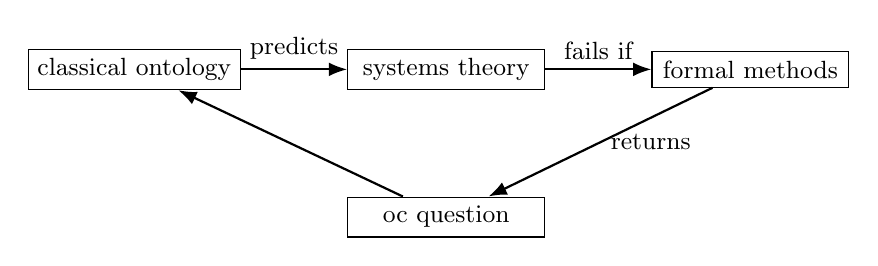
\begin{tikzpicture}[node distance=1.35cm,>=Latex,every node/.style={font=\small}]
\node[draw,align=center,minimum width=2.5cm] (c) {classical ontology};
\node[draw,align=center,minimum width=2.5cm,right=of c] (t) {systems theory};
\node[draw,align=center,minimum width=2.5cm,right=of t] (f) {formal methods};
\node[draw,align=center,minimum width=2.5cm,below=of t] (r) {oc question};
\draw[->,thick] (c) -- node[above]{predicts} (t);
\draw[->,thick] (t) -- node[above]{fails if} (f);
\draw[->,thick] (f) -- node[right]{returns} (r);
\draw[->,thick] (r) -- (c);
\end{tikzpicture}
\caption{Being to Substance in: falsifier of historical sequence pressure 11-1-6}
\label{fig:figure-from-being-to-substance-in-ancient-ontology-one}
\end{figure}
The point of the diagram is not decoration; it marks which relation is being proposed and which stronger conclusion is still unavailable.\par
A local clarification is useful here\par
A local clarification is useful here\footnote{In Being to Substance in, this note clarifies the reader clarification role of the term and keeps the caveat close to the sentence that needs it.}.\par
The note keeps the caveat near the term without derailing the main sentence.\par
The force of the problem can be felt in the contrast between permanence and flux. A radical language of flux makes the world vivid but threatens the possibility of stable knowledge. A radical language of permanence protects knowledge but threatens the credibility of experience. Ancient ontology develops in the tension between those poles. Its central achievement is not that it gives one final answer, but that it teaches later thought to distinguish several questions that had first appeared as one: what is, what changes, what remains, what can be known, and what kind of description fits the case.\par
A first-time reader does not need to inherit the ancient vocabulary as doctrine. The durable gain is simpler. The ancient debate shows that any serious account of the world must decide how it treats identity through variation. Without that decision, later claims about boundaries, continua, emergence, collapse, or transformation have no stable object. The river example is enough to show why. If the river is treated as nothing but its present water, then continuity vanishes. If it is treated as an unchanging object behind appearances, then flow becomes secondary. A usable ontology must hold together the fact that the river changes and the fact that it can still be tracked.\par
\section{What the Tradition Made Visible In Being to Substance in}
The ancient movement from being to substance can be read as a long attempt to make identity thinkable without denying change. Being names the widest question: what is it for anything to be? Substance narrows the question: what is the primary bearer of features, changes, and relations? The narrowing matters. A world described only in terms of being is too vast to guide ordinary inquiry. A world described through substances gives thought a working unit: this person, this tree, this horse, this artifact, this living body, this city. \cite{raf_networks,bak_soc}\par
Parmenides gives one powerful form to the problem. If what is not cannot be thought, then genuine being cannot come from non-being or pass into it. Change, in this frame, appears suspicious because it seems to require what is not yet or is no longer. Heraclitean language pushes in the opposite direction. Fire, flow, tension, and transformation become images for a world whose order is not static. The disagreement is often simplified into permanence against change, but its deeper lesson is that ontology must account for both the invariance required by thought and the variation disclosed by experience.\par
The local dependency can now be written without changing the claim it supports.\par
\begin{equation}\label{eq:equation-from-being-to-substance-in-ancient-ontology-two}
\operatorname{caseCoverage}_{2} = \tau_{\mathrm{repair}}=\inf\{t:C(t)<\theta\}
\end{equation}
The relation names a local dependency, variable dictionary, and proof/evidence role; it is not a claim-status upgrade.\par
The formula is a restraint on the prose. It names the dependency that the surrounding paragraph is allowed to use.\par
The comparison below gives being to substance in a set of quantities that can be inspected instead of merely admired.\par
\begin{table}[htbp]
\centering\small
\caption{Being to Substance in: observable quantities and counter-pressure 11-2-6}
\label{tab:table-from-being-to-substance-in-ancient-ontology-one}
\begin{tabular}{@{}llll@{}}
\toprule
Projection & Domain quantity & Comparator & Limit \\
\midrule
being to substance in boundary & 27 units & declared case & fixes what is compared \\
residual pressure & 0.63 & dimensionless & shows unresolved load \\
projection loss & 0.12 & bounded interval & marks lost structure \\
countercase set & 14 cases & review sample & keeps a falsifier visible \\
\bottomrule
\end{tabular}
\end{table}
The table should be read locally: it narrows the comparison without pretending that the wider theory has been settled by a single surface.\par
Plato's theory of Forms is one major response to this difficulty. A Form is not simply a mental idea. It is an intelligible pattern by which many changing things can be recognized as instances of the same kind. Beautiful things vary, deteriorate, and disagree with one another, but the question of beauty seems to reach beyond any single case. Plato protects intelligibility by placing the deepest stability outside the unstable sensible object. The sensible world participates in patterns it does not fully contain.\par
That account deserves more than a passing conversion into later vocabulary. Plato is not merely solving a technical problem about classification. He is asking how knowledge can rise above the instability of appearance without becoming empty. His answer binds ontology to education, mathematics, ethics, and the ordering of the soul. This chapter simplifies that larger architecture in order to isolate one thread: Plato's way of separating the intelligible stability of a kind from the changing instances through which it appears.\par
Aristotle shifts the weight back toward the concrete thing. The primary object of inquiry is not an otherworldly pattern alone, but a substance: a thing that bears properties and persists through certain kinds of change. A particular horse can grow, move, become sick, recover, and remain the same horse. It cannot, however, undergo every alteration and still remain what it is. Substance therefore introduces a disciplined relation between identity and allowable variation. It does not say that anything can change in any way. It says that some changes preserve the thing under description, while others destroy it or require another description.\par
Aristotle's doctrine is more intricate than the phrase working unit can capture. His Categories, his account of primary and secondary substance, and his later discussions of form, matter, actuality, and essence do not reduce to a single formula. Still, for the purpose of this chapter, one achievement is decisive: Aristotle gives inquiry a way to speak of a concrete bearer that is neither a bare lump of material nor a detached universal pattern. A horse is not only flesh and bone, and it is not only the general form horse. It is this organized living being.\par
The pair of matter and form is especially important. Matter is what a thing is made of; form is the organization or actuality by which that material is this kind of thing. Bronze can be statue, tool, coin, or lump. The material alone does not tell us which object is present. Form without material, at least for ordinary natural substances, does not give us the concrete thing either. The thing appears through their union. This distinction lets ontology talk about persistence without pretending that all persistence is material sameness.\par
The lineage also introduces potentiality and actuality. Potentiality names what a thing can become under the right conditions; actuality names what it is presently realized as. An acorn is not an oak tree, but it is not related to oakhood in the same way that a stone is. This distinction gives a vocabulary for directed possibility. Some futures belong to a thing's structure; others do not. Later theories of development, emergence, and transformation repeatedly return to this problem, even when they reject Aristotle's biology or metaphysics.\par
\section{Where the Inheritance Runs Out In Being to Substance in}
The model gained from ancient ontology is a grammar of stable reference under change. That grammar has three parts. First, it asks what counts as the object. Second, it asks which variations preserve that object. Third, it asks which variations require a new description. These questions are already present in ordinary judgment, but ancient ontology makes them explicit. A healed wound does not end a person. Death does. Repainting a ship does not end it. Burning it may. Replacing a plank may be minor; replacing every plank over time creates a harder case. The famous ship problem is not a puzzle for amusement. It shows that identity depends on rules of continuation, not on a single visible trait. \cite{raf_networks,bak_soc}\par
This gain matters for any later account of systems. A system cannot be analyzed unless it can be reidentified across time, perturbation, and observation. A system here means a structured ensemble whose parts, relations, and boundary conditions allow it to be described as one object for some purpose. The qualification matters: for some purpose. A forest, a nervous system, a legal institution, a supply chain, and a mathematical model are not the same kind of object. Yet each can be treated as a system if the description specifies what belongs to it, what relation organizes it, and what changes it can undergo without losing the relevant identity.\par
The local dependency can now be written without changing the claim it supports.\par
\begin{equation}\label{eq:equation-from-being-to-substance-in-ancient-ontology-one}
\operatorname{finiteCheck}_{2} = \operatorname{loss}_{\phi}=1-\frac{|E_{\phi}\cap E_{\mathrm{domain}}|}{|E_{\mathrm{domain}}|}
\end{equation}
The relation names a local dependency, variable dictionary, and proof/evidence role; it is not a claim-status upgrade.\par
The formula is a restraint on the prose. It names the dependency that the surrounding paragraph is allowed to use.\par
The local dependency can now be written without changing the claim it supports.\par
\begin{equation}\label{eq:equation-from-being-to-substance-in-ancient-ontology-three}
\operatorname{counterexamplePressure}_{2} = I_{\mathrm{axis}}=\frac{\operatorname{Var}(x\mid a)}{\operatorname{Var}(x)}
\end{equation}
The relation names a local dependency, variable dictionary, and proof/evidence role; it is not a claim-status upgrade.\par
The formula is a restraint on the prose. It names the dependency that the surrounding paragraph is allowed to use.\par
A small numerical test keeps the abstraction honest at the scale of a single decision.\par
\paragraph{Numerical example.} For being to substance in, take support=0.55, projection loss=0.13, and 6 open obligations. The bounded score is 0.; the example gives the reader a numeric scale without pretending to be empirical proof.\par
The numbers are deliberately small; their value is pedagogical, not evidential, unless the chapter binds them to a dataset elsewhere.\par
Modern network science offers a useful comparison, provided the comparison remains modest. Mark Newman's Networks: An Introduction, published in 2010, presents a general mathematical treatment of nodes, edges, connectivity, paths, communities, and dynamics across domains. Albert-Laszlo Barabasi's work, including Linked in 2002 and Network Science in 2016, helped popularize and formalize the study of networks with highly uneven connectivity, often discussed under the name scale-free networks. These works do not prove ancient ontology, and ancient ontology does not anticipate modern network theory. The connection is conceptual: both require a distinction between individual elements and the relational organization that makes an object describable as a structured whole.\par
The ancient matter-form distinction keeps that comparison disciplined. If a network is treated only as a list of nodes, its organization disappears. If it is treated only as an abstract pattern, its domain-specific constraints disappear. A protein interaction network, a social network, and a citation network may all be described with nodes and edges, but the meaning of a node and the meaning of an edge differs in each case. Newman's framework supports comparison, while the older discipline of substance and form warns against careless identification of unlike things. The same abstract relation can travel across domains only when its interpretation is named.\par
Boundaries then become more than lines drawn from outside. A boundary is a condition under which something can be counted as this object rather than that one. In a stone, the boundary appears spatially obvious. In a living organism, it is spatial, metabolic, immunological, and developmental. In a city, it is legal, infrastructural, economic, and lived. In a scientific model, it may be a declared domain of variables and assumptions. Ancient substance language does not solve all these cases, but it establishes the need to distinguish accidental variation from identity-altering change.\par
This is why substance remains valuable, if the word is used carefully. Substance has meant different things in Aristotle, scholastic metaphysics, early modern philosophy, and ordinary speech. The sense needed here is disciplined and limited: substance as a bearer of attribution, the something of which properties, changes, and relations are predicated. If a property is asserted, what has it? If a change occurs, what changes? If a relation is mapped, what relata are being related? If a contradiction appears, where is it located? These questions do not settle metaphysics, but they prevent language from drifting across objects without noticing.\par
\section{The Conceptual Debt In Being to Substance in}
The same model that gives stable reference also has limits. Substance language can make the world appear more object-like than it is. It favors bounded individuals, enduring bearers, and changes that happen to something already given. Many phenomena resist that pattern. Weather systems, markets, ecosystems, immune responses, scientific communities, and cultures are not easily described as substances in the classical sense. They have organization, persistence, and causal force, but their boundaries are distributed, porous, and sometimes dependent on the scale and purpose of observation. \cite{raf_networks,bak_soc}\par
The limit appears whenever process is not secondary to a thing but constitutive of the thing. A flame is not a lump that happens to burn; it is a maintained process of combustion. A whirlpool is not a hidden object wearing moving water as a costume; it is a dynamic pattern sustained by flow. A living organism is more substance-like than a whirlpool in many respects, yet its persistence also depends on continuous exchange with its environment. The organism remains itself by not remaining materially the same. Its identity is metabolic and organizational as much as material.\par
A small numerical test keeps the abstraction honest at the scale of a single decision.\par
\paragraph{Numerical example.} For being to substance in, take support=0.58, projection loss=0., and 1 open obligations. The bounded score is 0.260; the example gives the reader a numeric scale without pretending to be empirical proof.\par
The numbers are deliberately small; their value is pedagogical, not evidential, unless the chapter binds them to a dataset elsewhere.\par
The case that follows turns the proposal into a sequence of criticizable moves.\par
\paragraph{Worked case.} In the worked case for being to substance in, the claim is reduced to a boundary, an observable, a dependency, a numerical cue, and a falsifier. The case is useful only because each move can be criticized separately.\par
The case helps because each step can fail separately, which is exactly what a useful example should permit.\par
Ancient ontology contains resources for this problem, especially in Aristotle's attention to actuality, activity, and living form. Still, the inherited model often privileges a primary bearer beneath change. That tendency becomes restrictive when the object of inquiry is a pattern of relations, a regime of interaction, or a threshold phenomenon. A crowd panic, a financial cascade, or a phase transition cannot be understood merely by naming a substance and listing its properties. The relevant object may be the configuration itself.\par
Modern complexity language sharpens this limit, but it must be handled with care. Per Bak's How Nature Works, published in 1996, and the earlier work on self-organized criticality by Bak, Chao Tang, and Kurt Wiesenfeld in the late 1980s, examined model systems in which local interactions can produce states where events occur across many sizes. Barabasi's scale-free network models show how some networks with concentrated hubs may display robustness against certain random failures while remaining vulnerable to some targeted disruptions. These are model families and empirical research programs, not universal licenses to redescribe every phenomenon as critical, scale-free, or emergent.\par
Their usefulness here is limited but real. They show that relations, distributions, thresholds, and connection patterns can become primary objects of inquiry. A power grid makes this clear. It has physical components: generators, substations, transmission lines, control systems. Those components matter. Yet the grid's behavior cannot be read directly from any one component as a substance with properties. Stability depends on load, synchronization, control feedback, reserve capacity, and the pattern of interconnection. A failure may remain local, or it may cascade. The relevant identity of the grid is not exhausted by its material inventory. It is an organization operating under constraints.\par
This does not mean ancient ontology is obsolete. It means its strongest vocabulary must be placed within a wider descriptive frame. Substance asks what bears properties. Systems theory asks how parts and relations produce organized behavior. Network science asks how patterns of connection shape possible dynamics. Complexity theory asks how local rules, feedback, and thresholds may yield collective behavior. Each question adds something, and each can be abused if treated as a master key. The ancient model supplies the need for stable reference; its limit supplies the need for a broader language of organization.\par
\section{The Passage to Continua In Being to Substance in}
A successor framework becomes necessary when inherited concepts remain useful but no longer cover the cases that matter. The pressure after ancient ontology is not a rejection of being, form, substance, potentiality, or actuality. It is the demand to redescribe their work in terms that can handle layered systems, porous boundaries, changing observables, and domain-specific measures. The question shifts from what the primary substances are to how an object of inquiry is constituted, bounded, transformed, and compared. \cite{raf_networks,bak_soc}\par
This is a conceptual inheritance, not a direct historical genealogy. The claim is not that Parmenides, Plato, or Aristotle predicted network science, complexity theory, or contemporary systems language. They did not. The claim is that they clarified problems that return whenever thought tries to speak responsibly about persistence and change. Later vocabularies inherit the pressure of those problems even when they reject ancient answers.\par
In a substance-first description, one may begin by identifying the thing and then listing its properties. In a system-first description, one may need to identify a relation, a process, a boundary condition, or a scale before the thing becomes clear. A cell, for example, can be described as a bounded biological unit. But its relevant identity depends on membrane regulation, genetic expression, metabolism, signaling, and environment. No single inventory captures all of that.\par
The pressure also comes from multi-scale structure. A human body contains organs, tissues, cells, molecules, and microbial communities. It also participates in households, institutions, economies, and ecosystems. None of these levels can be reduced without remainder to the language of an isolated substance. Yet none can be responsibly described if identity dissolves into vague interconnection. The task is to preserve disciplined reference while allowing different scales to have different objects, measures, and modes of persistence.\par
Network examples clarify the point when kept within their scope. In a social network, a person may be a node. In a communication network, a device may be a node. In a citation network, a paper may be a node. Newman's general treatment helps compare such structures, while domain interpretation keeps the comparison from becoming empty. Barabasi's scale-free models add a further lesson: in some networks, the distribution of relations can matter as much as the intrinsic features of individual nodes. A highly connected hub is not merely a node with one more property; its position may alter the system's vulnerability and behavior.\par
The ancient term potentiality can also be carried forward with care. In modern system language, possibility is often constrained by structure. A dry forest has different fire potential from a wet one. A tightly coupled financial system has different cascade potential from a loosely coupled one. A network with concentrated hubs may have different failure modes from a more evenly connected network, depending on its domain and dynamics. These are not proofs of any one metaphysical thesis. They are reminders that what may happen is shaped by present organization, not by abstract possibility alone.\par
\section{A Problem Older Than the Vocabulary In Being to Substance in ontology}
In this book, Operational Coherence, abbreviated OC, names a proposed vocabulary for describing objects, systems, and transformations without assuming in advance that every object of inquiry is a classical substance. It begins from the lesson that being alone is too wide and substance alone is too narrow. Its concern is operational description: how to state what kind of object is under discussion, where its boundaries lie, what variations matter, what transformations occur, and how claims move across domains. \cite{raf_networks,bak_soc}\par
Several terms will become important. A continuum is a range of possible variation along which a system or feature can be described. A boundary is a condition that distinguishes inclusion from exclusion for a given description. An operator is a transformation rule or action that changes a configuration in a specified way. A projection is a disciplined translation of a description from one domain or level into another, with losses and constraints named rather than hidden. A contradiction is a structured incompatibility inside a description or configuration, not merely a feeling of tension. Collapse is the loss of organization required for the object to continue under the relevant description.\par
These terms inherit the ancient problem but change the working unit. Instead of asking only what substance bears a property, OC asks what configuration is being described, which continua are active, which boundaries define the object, and which operators transform it. This does not abolish substances. A substance-like object may be one case of a bounded configuration. But OC does not require all objects of inquiry to fit the model of a discrete enduring thing. A network, a process, a hierarchy, a regulatory loop, or a domain projection may also become the object of description if its identity conditions are stated.\par
The river can now be redescribed without losing the original problem. Its material flow changes continuously. Its channel, watershed, seasonal pattern, ecological role, legal designation, and cultural name may each provide a different continuity. No single description is automatically supreme. The correct description depends on the claim. If the claim concerns flood risk, the relevant continua include rainfall, saturation, channel capacity, land use, and flow rate. If the claim concerns legal jurisdiction, the relevant boundary may be administrative. If the claim concerns ecological health, species interaction and chemical composition enter. OC's task is to prevent these descriptions from being confused while allowing them to be related.\par
The bronze statue also becomes clearer. Matter persists across melting; statue-form does not. Some continua remain available, such as mass, chemical composition, or material source. Others terminate or shift, such as representational form, artistic integrity, or public object identity. The same event can preserve one description and destroy another. Ancient ontology already saw this through matter and form. OC generalizes the discipline by asking which boundaries and continua define each claim.\par
The power grid shows why the expansion is necessary. A grid is not only a collection of material components. It is a dynamic configuration whose stability depends on synchronized relations. An operator may be a load increase, a line failure, a control response, or a deliberate isolation procedure. A contradiction may arise when demand, transmission capacity, and control timing cannot be jointly satisfied under the current configuration. Resolution may require a new dimension of description, such as a finer control model, a different segmentation of the grid, or a new operating regime. Collapse, in the relevant sense, would be loss of coordinated service across the described system.\par
Such language risks becoming too general. If it can describe rivers, statues, organisms, cities, networks, and grids, perhaps it describes everything only by becoming vague. The answer must be operational constraint. A general vocabulary earns its use only when it forces sharper questions: What is the object? Which boundary is active? Which continuum is being varied? Which operator changes the configuration? Which projection is being made? What is preserved, what is lost, and what would refute the claim? Generality without such constraints is rhetoric. Generality with constraints can become comparison.\par
Ancient ontology has achieved something indispensable. It made being into a problem, distinguished stable reference from visible change, gave substance the role of disciplined bearer, and supplied matter, form, potentiality, and actuality as tools for thinking persistence and transformation. It cannot, by itself, handle every case in which identity is relational, layered, distributed, or threshold-dependent. The next step is therefore not to abandon the ancient question, but to carry it into a wider account of systems: one able to preserve the discipline of asking what is while also asking how organization holds, shifts, breaks, and becomes newly describable.\par
\chapter{Essence, Causality, and the Medieval to Modern Transition}
\section{A Problem Older Than the Vocabulary In Essence Causality Medieval to}
Before any scientific language can describe a system, it must decide what counts as a thing, where that thing begins and ends, what kind of change matters, and what can properly be called a cause. These decisions often remain quiet because mature sciences inherit working practices that make them seem obvious. A chemist, an ecologist, an engineer, and a historian do not usually begin by defending the meaning of object, boundary, or cause. They begin with a problem. Yet each problem already carries an ontology: a way of saying what exists for the purposes of explanation. \cite{bak_soc,newman_networks}\par
The medieval to modern transition matters because it makes this hidden decision visible. Medieval thought asked what a thing is, what form makes it the kind of thing it is, and how change can occur without destroying identity altogether. Modern science increasingly asked how change can be described through measurable relations, repeatable observations, and lawful dependence among states. The older vocabulary preserved the question of being. The newer vocabulary disciplined explanation by tying it to public procedures. Neither achievement cancels the other.\par
The next diagram slows the argument down just enough to show how essence causality medieval to is being organized.\par
\begin{figure}[htbp]
\centering
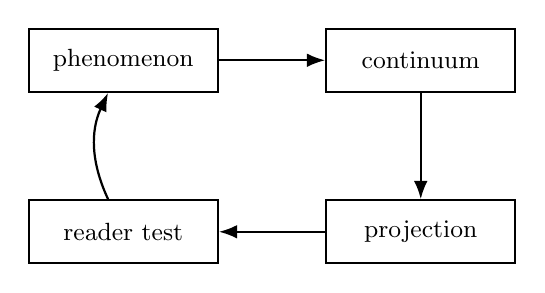
\begin{tikzpicture}[node distance=1.35cm,>=Latex,every node/.style={font=\small}]
\node[draw,thick,align=center,minimum width=2.4cm,minimum height=0.8cm] (a) {phenomenon};
\node[draw,thick,align=center,minimum width=2.4cm,minimum height=0.8cm,right=of a] (b) {continuum};
\node[draw,thick,align=center,minimum width=2.4cm,minimum height=0.8cm,below=of b] (c) {projection};
\node[draw,thick,align=center,minimum width=2.4cm,minimum height=0.8cm,left=of c] (d) {reader test};
\draw[->,thick] (a) -- (b);
\draw[->,thick] (b) -- (c);
\draw[->,thick] (c) -- (d);
\draw[->,thick,bend left=25] (d) to (a);
\end{tikzpicture}
\caption{Essence Causality Medieval to: state transition of conceptual dependency pressure 12-1-7}
\label{fig:figure-essence-causality-and-the-medieval-to-modern-transition-one}
\end{figure}
The point of the diagram is not decoration; it marks which relation is being proposed and which stronger conclusion is still unavailable.\par
A local clarification is useful here\par
A local clarification is useful here\footnote{In Essence Causality Medieval to, this note clarifies the reader clarification role of the term and keeps the caveat close to the sentence that needs it.}.\par
The note keeps the caveat near the term without derailing the main sentence.\par
A simple seed shows why the issue does not belong only to historians of philosophy. In one description, the seed is the kind of thing that can become a plant. It has a recognizable identity even while dormant. It is not a pebble, a crumb, or a speck of dust. In another description, the seed is a material configuration: coat, embryo, stored nutrients, genetic sequence, moisture content, and chemical state. In a third description, it belongs to a field, a season, a climate, a farmer's decision, a bird's appetite, a soil community, and a chain of reproduction. The seed is one small thing, but it draws several kinds of explanation toward itself.\par
The word essence names a claim about what something is across change. The word causality names a claim about how change happens. The difficulty begins when either word is treated as if it could be read directly from the world without specifying the scale and purpose of description. A seed is not a plant, yet it is not unrelated to the plant. A forest is not a pile of seeds, yet the forest depends on seed behavior, soil chemistry, rainfall, competition, fire, animals, and time. The same object can be stable under one description and transitional under another.\par
The historical question is therefore not decorative background. It is an early form of a problem later inherited by systems theory, ecology, network science, computation, and formal modeling. A theory that cannot distinguish kind, process, relation, scale, and operation will confuse explanation with naming. It may call something an essence when it has only found a repeated pattern. It may call something a cause when it has only measured a correlation. It may call something a system when it has only drawn a boundary. The book's vocabulary, called OC, begins from this danger: not by discarding older words, but by asking what work they are doing when they are used.\par
\section{What the Tradition Made Visible In Essence Causality Medieval to}
Medieval ontology inherited an ancient concern with being, form, substance, and cause. Substance named what exists in its own right rather than merely as a feature of something else. Form named the organizing pattern by which a thing is the kind of thing it is. Cause did not mean only a prior mechanical push. In the Aristotelian tradition, a full explanation could include the material out of which something is made, the form that organizes it, the agent that brings it about, and the end or use toward which its development or making tends. \cite{bak_soc,newman_networks}\par
The familiar example of a house remains useful because it is ordinary. The timber, stone, brick, glass, steel, and wiring are material causes. The arrangement that makes these materials a house rather than a heap is the formal cause. The builders, tools, plans, permissions, labor, and sequence of construction are efficient causes. Habitation is the final cause, not because every beam secretly wants shelter, but because the structure is intelligible as a house only through the use it is ordered to serve. One building can carry several explanatory roles at once.\par
The local dependency can now be written without changing the claim it supports.\par
\begin{equation}\label{eq:equation-essence-causality-and-the-medieval-to-modern-transition-two}
\operatorname{transitionThreshold}_{2} = \rho_{\mathrm{replay}}=\frac{N_{\mathrm{matched}}}{N_{\mathrm{declared}}}
\end{equation}
The relation names a local dependency, variable dictionary, and proof/evidence role; it is not a claim-status upgrade.\par
The formula is a restraint on the prose. It names the dependency that the surrounding paragraph is allowed to use.\par
The comparison below gives essence causality medieval to a set of quantities that can be inspected instead of merely admired.\par
\begin{table}[htbp]
\centering\small
\caption{Essence Causality Medieval to: observable quantities and counter-pressure 12-2-7}
\label{tab:table-essence-causality-and-the-medieval-to-modern-transition-one}
\begin{tabular}{@{}llll@{}}
\toprule
Proof object & Dependency & Lean surface & Closure state \\
\midrule
essence causality medieval to boundary & 30 units & declared case & fixes what is compared \\
residual pressure & 0.70 & dimensionless & shows unresolved load \\
projection loss & 0.23 & bounded interval & marks lost structure \\
countercase set & 15 cases & review sample & keeps a falsifier visible \\
\bottomrule
\end{tabular}
\end{table}
The table should be read locally: it narrows the comparison without pretending that the wider theory has been settled by a single surface.\par
The same style of thought could be extended to organisms, artifacts, institutions, and natural processes. A tree was not merely a column of matter. It had a form through which matter was organized into a living thing. A craft object was not merely shaped stuff. It belonged to a practice, a use, and a pattern of making. A human action could be described through material conditions, intention, agency, and end. This older grammar was often entangled with theological and hierarchical assumptions, but it also preserved a subtle insight: ordinary things are not exhausted by listing their parts.\par
The modern transition did not simply refute this scheme. It changed the public authority of explanation. As experimental mechanics, mathematical physics, and instrument-based inquiry matured, causes became increasingly associated with lawful relations among measurable states. Galileo's inclined planes, Boyle's air pump, Newton's mechanics, and later laboratory practices shifted trust toward what could be isolated, measured, repeated, and expressed with mathematical discipline. A falling stone, a pendulum, a pressure system, or an orbit could be described without appealing to the inward purpose of the object.\par
This was an immense gain. It made prediction, replication, and engineered intervention possible at a scale older explanatory habits could not match. Modern science could ask what variables changed, what remained invariant, what law related one state to another, and what experiment could expose the difference between a plausible story and a reliable result. It did not need to know the essence of a pendulum in order to model its period. It did not need to attribute purpose to a planet in order to calculate an orbit.\par
The cost was not always noticed at once. When explanation is restricted to measurable relation, the status of essence becomes unstable. Is essence a real feature of things, a classification made by observers, a convenient compression of regular behavior, or a residue of obsolete metaphysics? Modern science often succeeds by refusing to answer that question directly. It classifies by function, structure, lineage, measurement, and model fit. Yet the question returns whenever a system changes its organization while remaining identifiable as the same system.\par
A living organism makes the return unavoidable. Its matter is exchanged continuously. Its cells divide, die, regenerate, and specialize. Its immune system learns from exposure. Its metabolism depends on an environment it does not fully control. Its behavior changes with injury, age, stress, memory, nutrition, and social context. If identity meant identical material composition, the organism would vanish into flux. If identity meant a fixed hidden essence untouched by process, development would become unintelligible. The organism persists by organized change.\par
Medieval language would be tempted to speak of form or essence. Modern language speaks of organization, regulation, development, homeostasis, adaptation, and system state. The vocabularies differ, but the underlying demand remains: how can continuity persist through change? The answer cannot be found by retreating into a single inherited word. It has to specify what remains continuous, what is allowed to vary, what boundary is being drawn, and what kind of transformation counts as preserving the thing rather than destroying it.\par
This is where ontology and metaontology must be distinguished. Ontology asks what kinds of things there are, or what must be said to exist within a given account. Metaontology asks how those claims are being made: what categories, distinctions, and operations allow something to appear as an object, process, relation, or event in the first place. The distinction matters because many modern objects of inquiry are not substances in the older sense. A feedback loop, a market signal, a pressure gradient, a network cluster, and a developmental pathway are all real enough for disciplined inquiry, but their reality is tied to how they are detected, modeled, and used.\par
OC does not revive medieval metaphysics as doctrine, and it does not treat modern mechanism as sufficient for every domain. It takes the transition as a lesson in description. Older ontology preserved the question of what makes something the kind of thing it is. Modern science disciplined explanation through measurement, relation, and reproducibility. A usable metaontology has to keep the question and the discipline together without confusing one for the other.\par
\section{Where the Inheritance Runs Out In Essence Causality Medieval to}
The modern gain is operational clarity. An operational description states how something is distinguished, measured, transformed, or compared. It does not begin by asking for the hidden essence of a thing. It asks what can be done with the distinction and what remains stable when the operation is repeated. In this sense, an operation is a rule-governed act of description or transformation: counting, measuring, mapping, sorting, perturbing, projecting, or comparing according to explicit conditions. \cite{bak_soc,newman_networks}\par
This shift matters because many scientific objects are not visible substances in the older sense. A temperature field is not a thing one can hold. A pressure gradient is not an object standing alone. An attractor is a pattern in a space of possible states. A feedback loop is a relation through which output returns as input. A network cluster is a structure of connection among defined units. These objects are not imaginary because they are operational. They are constrained by measurement, representation, and repeated use.\par
The local dependency can now be written without changing the claim it supports.\par
\begin{equation}\label{eq:equation-essence-causality-and-the-medieval-to-modern-transition-one}
\operatorname{operatorBurden}_{2} = G=(V_{\mathrm{claim}}\cup V_{\mathrm{evidence}},E_{\mathrm{support}}\cup E_{\mathrm{challenge}})
\end{equation}
The relation names a local dependency, variable dictionary, and proof/evidence role; it is not a claim-status upgrade.\par
The formula is a restraint on the prose. It names the dependency that the surrounding paragraph is allowed to use.\par
The local dependency can now be written without changing the claim it supports.\par
\begin{equation}\label{eq:equation-essence-causality-and-the-medieval-to-modern-transition-three}
\operatorname{graphWalk}_{2} = \epsilon_{\mathrm{domain}}=\max_i |y_i-\hat y_i|
\end{equation}
The relation names a local dependency, variable dictionary, and proof/evidence role; it is not a claim-status upgrade.\par
The formula is a restraint on the prose. It names the dependency that the surrounding paragraph is allowed to use.\par
A small numerical test keeps the abstraction honest at the scale of a single decision.\par
\paragraph{Numerical example.} For essence causality medieval to, take support=0.61, projection loss=0.11, and 2 open obligations. The bounded score is 0.167; the example gives the reader a numeric scale without pretending to be empirical proof.\par
The numbers are deliberately small; their value is pedagogical, not evidential, unless the chapter binds them to a dataset elsewhere.\par
Network science gives a clear example. A network is a structure made of nodes and links. A node is the unit being related; a link is the relation between units. The identity of a network feature depends less on the intrinsic essence of a single node than on the pattern of connections among nodes. Mark Newman has shown how many systems can be studied by representing relations among units and then asking how global structure follows from local connection patterns. The method can apply to social ties, power grids, biological interactions, citations, transport systems, and digital communication.\par
This does not abolish ontology. It relocates it. The question becomes: what is being counted as a node, what counts as a link, and what operation preserves the pattern being studied? In a social network, a node might be a person, an institution, a document, or an event. A link might mean friendship, citation, money flow, co-presence, influence, or shared membership. The same real-world situation can generate different networks depending on the operation that defines relation.\par
Albert-Laszlo Barabasi's work on scale-free networks sharpened the point by showing that some networks contain highly connected hubs and many sparsely connected nodes. The model does not require each node to have a medieval essence in order to explain a structural feature. It shows how growth and preferential attachment can yield a recognizable distribution. A pattern can therefore become explanatorily serious without being a substance.\par
The seed can now be seen under a different light. In a field, a seed is not only an individual biological object. It can be a unit in a dispersal network, a carrier in a genetic lineage, a point in a supply chain, a potential plant in a crop model, or a food source in an ecological relation. Each description makes something real for inquiry by defining units and relations. A bird eating the seed, a farmer storing it, a fungus attacking it, and a geneticist sequencing it do not encounter four unrelated worlds. They encounter the same material configuration through different operations.\par
The power of operational description lies in this discipline. It can say what is being held constant and what is being allowed to vary. It can say which boundary matters for the question at hand. A boundary is a distinction that separates, relates, or transforms regions of description: seed and soil, organism and environment, city and region, model and measurement. A continuum is a structured range of variation in which positions can differ without becoming unrelated: dry to hydrated, dormant to germinating, local heat to regional climate, individual behavior to population distribution. A level is a chosen scale or layer of description, such as molecular, organismic, ecological, institutional, or computational.\par
Once these terms are introduced, the seed example becomes sharper rather than heavier. The seed can be described along a biological continuum of development, across a boundary between dormant and germinating states, and under operations such as hydration, temperature change, metabolic activation, and gene expression. The older language of potential plant life is not simply discarded. It is translated into conditions, transformations, and continuities that can be examined at specified levels.\par
Modern explanation therefore gives OC one of its essential constraints. It is not enough to say that a thing has an essence. It is necessary to ask what features persist under what transformations. It is not enough to say that something causes something else. It is necessary to ask what relation, intervention, model, or observed dependence justifies the claim. It is not enough to say that a system exists. It is necessary to ask what boundary has been drawn and what operations keep the system identifiable.\par
The scientific object becomes partly made by the measurement practice, the mathematical representation, and the stability of the result across cases. Partly made does not mean fabricated. A thermometer does not invent heat by measuring temperature. A network diagram does not invent relations by representing them. But the form in which a phenomenon becomes available to inquiry depends on the operation through which it is described. That dependence is not a weakness. It is the beginning of discipline.\par
\section{The Conceptual Debt In Essence Causality Medieval to}
Operational clarity also has a limit. If every object is defined only by the operation that detects it, the same thing can fragment into unrelated descriptions. The seed becomes a genetic sequence for one inquiry, a unit of agricultural yield for another, a food source for another, a dispersal mechanism for another, and a node in an ecological network for another. Each description can be useful. Usefulness alone does not explain how the descriptions relate. \cite{bak_soc,newman_networks}\par
The older problem of being returns in a modern form. A system is not merely a list of measurements. It has some pattern of persistence, some range of admissible change, and some way of failing to remain what it was. The problem is not that modern models lack rigor. The problem is that rigor inside one model does not automatically give a language for relating models across levels. A measurement can be exact and still leave the larger identity of the system unclear.\par
A small numerical test keeps the abstraction honest at the scale of a single decision.\par
\paragraph{Numerical example.} For essence causality medieval to, take support=0.44, projection loss=0.16, and 3 open obligations. The bounded score is 0.; the example gives the reader a numeric scale without pretending to be empirical proof.\par
The numbers are deliberately small; their value is pedagogical, not evidential, unless the chapter binds them to a dataset elsewhere.\par
The case that follows turns the proposal into a sequence of criticizable moves.\par
\paragraph{Worked case.} In the worked case for essence causality medieval to, the claim is reduced to a boundary, an observable, a dependency, a numerical cue, and a falsifier. The case is useful only because each move can be criticized separately.\par
The case helps because each step can fail separately, which is exactly what a useful example should permit.\par
Ecology makes the difficulty vivid. Robert May's work on stability and complexity challenged the assumption that more complex ecological networks are automatically more stable. The finding mattered because it showed that intuitive appeals to richness, balance, or organic wholeness can fail under mathematical analysis. A community with many interactions is not automatically protected by its complexity. Under some modeled conditions, complexity can make stability harder rather than easier.\par
Yet the result also depends on how species, interactions, strengths, and perturbations are represented. Which species count as units? Which interactions count as links? Are interaction strengths fixed, variable, seasonal, or context-dependent? What kind of disturbance is being introduced, and at what scale? The lesson is not that mathematics dissolves ontology. The lesson is that formal models can correct metaphysical intuition while model construction still carries ontological commitments.\par
The seed in the field belongs to this difficulty. Its fate depends not only on internal structure but on relations that are uneven in strength and timing. Moisture may awaken it. Too much moisture may rot it. A warm spell may trigger germination before a frost. A bird may carry it beyond the parent plant's shadow. A farmer may select it for yield, uniformity, drought tolerance, or market demand. The seed's identity as a seed is stable enough for ordinary speech, but its explanatory role changes as the surrounding system changes.\par
Self-organized criticality offers another image. Per Bak's sandpile model became famous because it captured the difference between local addition and system-wide reconfiguration. One grain may do little. Another grain may trigger an avalanche. The event cannot be understood by inspecting the grain alone. It depends on the state of the whole pile: slope, accumulation, friction, previous falls, and the nearness of the system to a threshold.\par
The limit of a purely object-centered ontology is obvious here. The avalanche is not the essence of the grain, and it is not an external miracle. It is a system-level event made possible by accumulated configuration. The limit of a purely relation-centered ontology is also visible. Not every relation matters in the same way, and not every perturbation has the same effect. The system requires a vocabulary for stored tension, threshold, boundary, and transformation.\par
A contradiction, in the sense needed here, is not merely a logical error or a rhetorical clash. It is a configuration in which descriptions, constraints, or tendencies cannot all remain satisfied under the current organization. A seed cannot remain dormant and germinate in the same respect at the same level of description. A city cannot keep adding heat, electrical demand, medical strain, and infrastructure fragility indefinitely while preserving the same pattern of functioning. An ecological model cannot treat interaction strengths as both irrelevant and decisive without changing what is being claimed.\par
Some contradictions are failures of speech and should simply be corrected. Others reveal that a description has reached its limit. If one account of the seed treats it only as a static object, germination appears as a replacement of one thing by another. If another account treats it only as continuous process, the boundary between seed and plant may become too vague for agricultural, biological, or legal purposes. The pressure is not solved by choosing one description as always superior. It is solved by specifying the level at which each claim holds and the transformation by which one description gives way to another.\par
This is why contradiction becomes an organizing pressure rather than one phenomenon among many. It marks the place where a description can no longer preserve all of its commitments at once. Sometimes the configuration collapses: the organism dies, the model fails, the institution breaks, the sandpile avalanches. Sometimes a new dimension of description is required: development rather than object, network rather than individual, threshold rather than linear accumulation, projection rather than simple analogy. The claim is not a universal law already proven across all domains. It is a disciplined way to notice where explanation is being forced to change form.\par
The medieval-modern transition prepares the reader for this caution. Medieval essence-language can overstate unity. Modern operational language can overfragment unity. Systems language can overgeneralize pattern. Network language can overprivilege connection. Mathematical elegance can hide modeling choices. OC is designed to make those choices explicit, not to pretend that a single inherited vocabulary already solves them.\par
\section{The Passage to Continua In Essence Causality Medieval to}
A new coordinating vocabulary becomes useful when inherited vocabularies each preserve part of the problem while failing to coordinate the whole. Essence preserves continuity across change. Causality preserves transformation and dependence. Mechanism preserves lawful relation. Network theory preserves structure among units. Complexity theory preserves emergence, threshold, and cascade. None of these alone supplies a complete public language for comparing systems whose boundaries, levels, and observables shift across domains. \cite{bak_soc,newman_networks}\par
The pressure is practical before it is theoretical. Consider a city during a heat wave. The city is a physical environment, an infrastructure network, an administrative object, a population distribution, an economic system, and a lived social reality. Heat moves through asphalt, concrete, glass, soil, shade, air, pipes, and rooms. Electrical demand rises as cooling systems work harder. Transit reliability may shift as tracks, roads, engines, and schedules respond to temperature. Hospital admissions may rise. Outdoor labor becomes more dangerous. Neighborhoods with fewer trees, poorer housing, older residents, or weaker services may suffer more severely.\par
No single description is false simply because it is incomplete. A meteorologist may describe the heat dome and atmospheric pattern. An engineer may describe grid load and equipment limits. A public health worker may describe vulnerable populations and emergency response. An economist may describe lost productivity and energy prices. A resident may describe the impossibility of sleep in a top-floor apartment. The city is not one object in the old substance sense, yet it is not a mere heap of unrelated facts. It is a coordinated site where different continua cross.\par
Calling the city a substance is too blunt. Calling it a network is useful but incomplete, because the relevant nodes and links differ by question. In the electrical grid, nodes may be substations, generators, transformers, and households. In public health, nodes may be clinics, neighborhoods, ambulance routes, or demographic groups. In transportation, nodes may be stations, intersections, depots, and bottlenecks. The word network becomes explanatory only when the units and relations have been specified.\par
Calling the city a complex system is directionally right but too broad unless the terms are disciplined. Complexity may refer to many interacting parts, nonlinear response, adaptive behavior, emergent pattern, computational difficulty, institutional fragmentation, or historical layering. These meanings overlap but are not identical. A heat wave forces the distinction because a failure in one layer can become a pressure in another. A stressed electrical grid changes the health situation. A health emergency changes administrative priorities. Administrative delay changes exposure. Exposure changes social trust.\par
The city therefore makes metaontology concrete. Metaontology is not a remote philosophical exercise. It asks what kind of descriptive machinery is being used when existence, identity, boundary, change, and cause are asserted. When we say the city is overheating, what is the subject of the sentence? Air temperature, surface temperature, energy demand, human bodies, institutions, buildings, neighborhoods, or the coupled pattern among them? The answer depends on the operation being performed: measurement, mapping, forecasting, intervention, comparison, or accountability.\par
OC makes level and projection explicit. A level is a chosen scale or layer of description: material surface, building, neighborhood, infrastructure network, population, institution, or regional climate. A projection is a disciplined mapping from one level or descriptive frame into another. A projection never carries everything. It preserves some relations and loses others. A map of surface temperature may project thermal exposure into geographic space while losing household income, medical vulnerability, and social isolation. A hospital admission model may project bodily stress into public health categories while losing the material history of housing and shade.\par
This is why cross-domain comparison requires rules rather than metaphor alone. It may be tempting to say that a city is like an organism, a network, a machine, or a sandpile. Each metaphor can reveal something. The city has flows, dependencies, thresholds, repair processes, and cascades. But each metaphor also misleads if allowed to govern the whole description. A city does not have one metabolism in the biological sense. It is not designed like a machine from a single plan. Its residents are not grains of sand. Its neighborhoods are not organs with fixed functions.\par
The test of OC's vocabulary is whether it prevents bad inference. A network hub may be causally important in one model, but it does not follow that the same hub is the essence of the system. A stable ecological pattern may persist across disturbances, but it does not follow that complexity guarantees stability. A cascade may begin with a small event, but it does not follow that small events generally have large effects. A city map may show a hot neighborhood, but it does not follow that temperature alone explains vulnerability.\par
The answer is not to eliminate ordinary language. Essence, cause, system, boundary, and emergence remain useful words when handled with discipline. The answer is to specify the operation being performed when those words appear. Is the claim about identity through change, lawful dependence, relation among units, threshold behavior, model transfer, or projection across domains? OC earns its place only if it makes those questions harder to evade.\par
\section{A Problem Older Than the Vocabulary In Essence Causality Medieval to transiti}
The historical transition has now done its work. It has shown why essence cannot simply be abandoned, because continuity through change remains a real explanatory need. It has shown why causality cannot be left in a loose metaphysical state, because change must be accountable to observation, relation, and model. It has also shown why later sciences of networks and complexity matter: many important objects are patterns of organization rather than isolated substances. \cite{bak_soc,newman_networks}\par
OC begins from three commitments. First, no domain receives automatic authority over all others. Biology, physics, computation, social theory, mathematics, and history do not share all observables or all standards of explanation. Second, comparison across domains is possible when the terms of projection are explicit. Third, unresolved contradiction should be treated as a structured event in description, not as an invitation to inflated language.\par
The central hypothesis can now be stated plainly: an unresolved contradiction either gives rise to a new dimension of description or collapses the configuration that cannot resolve it. The sentence is not offered as a completed empirical law over all possible systems. It is an organizing proposal that later vocabulary, examples, models, and domain projections must narrow, test, and sometimes reject.\par
Return to the seed one last time. At the level of ordinary identity, the seed is one thing and the plant another. At the developmental level, the seed and plant belong to one process. At the ecological level, the seed is part of reproduction, dispersal, predation, competition, and soil exchange. At the agricultural level, it may be part of yield management, storage, selection, trade, and risk. A contradiction appears if one description is forced to do all the work. The solution is not to choose one level as the only real one. The solution is to state the level, boundary, continuum, operation, and projection involved.\par
This does not make every perspective equally strong. Some projections are lossy in ways that matter. Some models fail. Some analogies are decorative. Some claims cannot be carried from one domain to another. A projection from ecological stability to institutional stability, for example, cannot borrow May's result as if social institutions were species in a food web. It can only ask whether an analogous structure has been defined, whether its units and relations are specified, and whether the comparison survives scrutiny.\par
The same restraint applies to network language. Newman and Barabasi help show why relation and topology matter, but a network diagram is not automatically an explanation. A hub, cluster, path length, or degree distribution becomes explanatory only when the nodes and links have been defined in relation to a real question. A transit hub, a financial hub, a social hub, and a biological hub do not become the same kind of cause because they share a diagrammatic form.\par
The same restraint applies to cascade language. Bak's sandpile gives a powerful image for threshold behavior, but not every crisis is a sandpile and not every accumulation produces a critical state. OC can use the distinction between local perturbation and system-level reconfiguration while leaving domain-specific validation to the domains themselves. The point is not to make one model travel everywhere. The point is to know what has traveled when a model moves.\par
The city under heat makes the same discipline visible at a larger scale. If a transformer fails during peak demand, the failure may be local in equipment terms but regional in social consequence. If a cooling center opens far from the most vulnerable residents, an administrative solution may fail at the level of mobility. If a shaded neighborhood remains cooler, the cause is not only trees in the abstract but the historical pattern that allowed canopy, wealth, maintenance, and land use to accumulate together. Description has to move, but it has to move with declared losses.\par
This is the handoff from history to theory. Essence and causality do not disappear. They become disciplined questions inside a larger operational grammar. What remains continuous? What produces change? What boundary is being drawn? What level is active? What transformation is allowed? What projection is being made? What happens when the description can no longer hold together?\par
The medieval inheritance keeps the question of being alive. The modern inheritance insists that explanation submit to public discipline. Network and complexity sciences show that relation, distribution, threshold, and cascade can be real objects of inquiry without becoming substances in the old sense. OC enters after these lessons, not before them. Its task is to give the next chapters a language for saying how systems persist, change, break, and sometimes require a new dimension of description before they can be understood at all.\par
\chapter{Kant, Hegel, and the Problem of Contradiction}
\section{A Problem Older Than the Vocabulary In Kant Hegel Problem of}
Being first appears to thought as the simplest possible word and then immediately ceases to be simple. To say that something is seems plain enough when the example is a stone on a table, a body in motion, or a storm seen from a window. The difficulty begins when the same word is asked to cover a promise, a legal border, a temperature gradient, a species, a market panic, a theorem, and a self-correcting machine. Each is real in some sense, but not in the same way. A stone resists the hand. A border organizes conduct. A gradient drives change. A theorem constrains inference. A panic spreads through expectation. If all are called beings without distinction, the word becomes too loose. If only one mode is admitted as truly real, the world is flattened to fit a prior preference. \cite{newman_networks,barabasi_scale_free}\par
The problem of being is therefore not a taste for abstraction. It is the practical difficulty of saying what kind of thing is under discussion before claims about it become meaningful. A first-time reader can begin with a river. The river is water, but not only water. It has banks, a bed, currents, sediment, seasonal variation, ecological relations, legal names, engineering interventions, and memories in the communities around it. A child may know it as a place to fish. A city may know it as a line on a flood map. An engineer may know it by volume, velocity, and load. An ecologist may know it by spawning grounds, invasive species, and oxygen levels. None of these descriptions is simply false, yet none is the river by itself.\par
The next diagram slows the argument down just enough to show how kant hegel problem of is being organized.\par
\begin{figure}[htbp]
\centering
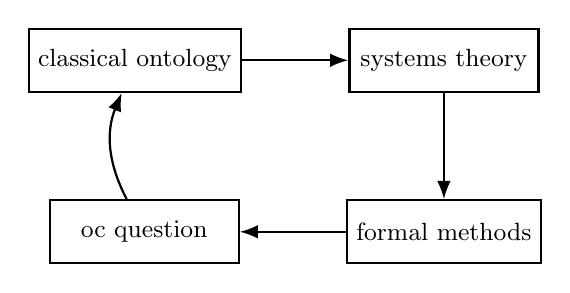
\begin{tikzpicture}[node distance=1.35cm,>=Latex,every node/.style={font=\small}]
\node[draw,thick,align=center,minimum width=2.4cm,minimum height=0.8cm] (a) {classical ontology};
\node[draw,thick,align=center,minimum width=2.4cm,minimum height=0.8cm,right=of a] (b) {systems theory};
\node[draw,thick,align=center,minimum width=2.4cm,minimum height=0.8cm,below=of b] (c) {formal methods};
\node[draw,thick,align=center,minimum width=2.4cm,minimum height=0.8cm,left=of c] (d) {oc question};
\draw[->,thick] (a) -- (b);
\draw[->,thick] (b) -- (c);
\draw[->,thick] (c) -- (d);
\draw[->,thick,bend left=25] (d) to (a);
\end{tikzpicture}
\caption{Kant Hegel Problem of: residual plot of historical sequence pressure 13-1-8}
\label{fig:figure-kant-hegel-and-the-problem-of-contradiction-one}
\end{figure}
The point of the diagram is not decoration; it marks which relation is being proposed and which stronger conclusion is still unavailable.\par
A local clarification is useful here\par
A local clarification is useful here\footnote{In Kant Hegel Problem of, this note clarifies the reader clarification role of the term and keeps the caveat close to the sentence that needs it.}.\par
The note keeps the caveat near the term without derailing the main sentence.\par
Remove the flowing water and the river is gone in one sense. Remove the name and maps and the river remains in another. Dam it, divert it, poison it, restore it, and the answer to what the river is changes according to the question being asked. The river teaches a modest but severe lesson: an entity is not always exhausted by its material contents, and a name is not always an empty addition to matter. Some things exist as organized processes. Some exist as relations. Some exist as rules that alter behavior. Some exist as patterns that persist through replacement of parts. The word being must be able to carry these differences without dissolving them.\par
This is the need for a metaontology. An ontology gives an account of what kinds of things there are. A metaontology asks how such accounts are formed, limited, compared, and made usable when different domains do not present the same kinds of objects. It does not begin by listing stones, rivers, laws, markets, organisms, and machines as if the list itself solved the problem. It asks what must be specified for any such listing to make sense. What counts as a boundary? What counts as continuity? What counts as change? What counts as the same thing persisting through alteration?\par
The river is not a trick example; it is a normal one. It shows why being cannot be treated only as a list of entities. It must also be treated through boundaries, continuities, operations, and transformations. A river has edges, but its edges shift. It has identity, but its matter is constantly replaced. It has measurable flow, but also legal and social consequences. To describe it well is not to choose one register and abolish the others. It is to know which register is doing which work.\par
The ontological continuum begins from this difficulty. It does not declare that every system is the same kind of object. It asks how a system can be described without losing the differences that make it what it is. That question places the old philosophical problem of being under a newer pressure: not merely what exists, but how different modes of existence can be spoken of together without confusion.\par
\section{What the Tradition Made Visible In Kant Hegel Problem of}
Kant enters this problem by changing the question from what reality is in itself to how experience becomes intelligible to a finite knower. In the critical philosophy, the mind is not a blank surface on which the world merely writes. Experience is structured. Space and time are not discovered in the same way that a tree or a planet is discovered; they are forms under which objects can appear to us at all. Categories such as causality are not optional decorations added after perception. They are part of the form through which a sequence can be recognized as an event rather than as an unconnected succession. \cite{newman_networks,barabasi_scale_free}\par
This does not make the world imaginary. Kant's discipline is sharper than that. The point is that claims about objects must pass through the conditions of possible experience. The thing as it is independently of those conditions is not denied, but it is not available as an object of ordinary knowledge in the same way that appearances are. The result is a profound boundary in philosophy: knowledge has reach, but also form; reason has power, but also limits. A claim that ignores those limits may sound grand while losing its right to be called knowledge.\par
The local dependency can now be written without changing the claim it supports.\par
\begin{equation}\label{eq:equation-kant-hegel-and-the-problem-of-contradiction-two}
\operatorname{reviewClosure}_{2} = \kappa_{K_2}=\frac{b_{K_2}+s_{K_2}}{1+o_{K_2}+q_{K_2}}
\end{equation}
The relation names a local dependency, variable dictionary, and proof/evidence role; it is not a claim-status upgrade.\par
The formula is a restraint on the prose. It names the dependency that the surrounding paragraph is allowed to use.\par
The comparison below gives kant hegel problem of a set of quantities that can be inspected instead of merely admired.\par
\begin{table}[htbp]
\centering\small
\caption{Kant Hegel Problem of: observable quantities and counter-pressure 13-2-8}
\label{tab:table-kant-hegel-and-the-problem-of-contradiction-one}
\begin{tabular}{@{}llll@{}}
\toprule
Dataset role & Source type & Replay cue & Reader question \\
\midrule
kant hegel problem of boundary & 33 units & declared case & fixes what is compared \\
residual pressure & 0.77 & dimensionless & shows unresolved load \\
projection loss & 0.34 & bounded interval & marks lost structure \\
countercase set & 16 cases & review sample & keeps a falsifier visible \\
\bottomrule
\end{tabular}
\end{table}
The table should be read locally: it narrows the comparison without pretending that the wider theory has been settled by a single surface.\par
For the present argument, Kant matters because he prevents being from becoming a word without conditions. To speak about an object is already to speak within a frame that makes objecthood possible. A body is not merely a sensation; it is something located in space, enduring through time, capable of causal relation, and available under rules of judgment. If those conditions are ignored, a sentence may still appear philosophical, but its object begins to blur. Kant's question is not only what is being asserted, but under what conditions such an assertion can count as knowledge.\par
Contradiction, for Kant, becomes especially important where reason exceeds the conditions under which its concepts can be legitimately used. In the antinomies, reason generates opposing claims that both seem compelling when applied beyond possible experience. The world must have a beginning in time; the world cannot have a beginning in time. Every composite substance is made of simple parts; no composite thing is made of simple parts. These conflicts are not mere mistakes of arithmetic. They show what happens when reason treats its demand for completeness as if it already possessed the object that would satisfy it.\par
Hegel accepts the seriousness of contradiction but refuses Kant's final border between knowing and what lies beyond knowing. For Hegel, contradiction is not simply a warning sign that thought has overreached. It can be the pressure by which a concept reveals its inadequacy. A concept is not fully known by stating its definition at rest. It must be followed through the tensions it generates when it tries to account for its object. The history of thought, social life, and self-consciousness becomes a history of forms that discover their own limits and pass into altered forms.\par
The word dialectic names this movement of concepts through opposition, instability, and transformation. In weak usage, dialectic is sometimes reduced to a three-step slogan: thesis, antithesis, synthesis. That slogan is too crude for the work needed here. The important point is not a mechanical sequence of three labels. It is that a form of thought can contain a conflict that is not accidental to it. The conflict may disclose what the form cannot yet say. The next form is not merely a compromise between two opinions; it is an altered field in which the earlier opposition can be understood differently.\par
Kant and Hegel therefore stand at two necessary extremes. Kant teaches that intelligibility depends on conditions, and that reason must account for its own limits. Hegel teaches that limits may not be inert borders; they may become active pressures within the life of a form. The ontological continuum does not simply adopt either system. It receives the problem they sharpened: how can one speak about contradiction without treating it as a mere error, and without romanticizing it as automatic progress?\par
\section{Where the Inheritance Runs Out In Kant Hegel Problem of}
From Kant comes a disciplined suspicion of unframed claims. A claim never arrives from nowhere. It arrives inside a domain of possible observation, a vocabulary, a set of distinctions, and a rule for what counts as an object. In natural science, this is familiar. A temperature field, a genetic sequence, and a graph of social ties are not interchangeable observables. Each requires instruments, conventions, and rules of interpretation. Kant's deeper lesson is that this dependence is not an embarrassment. It is part of what makes knowledge possible. \cite{newman_networks,barabasi_scale_free}\par
The same lesson applies outside science. A contract, a law, a marriage, a debt, and a citizenship are not objects in the same way that stones are objects. They may have documents attached to them, but the document is not the whole reality. Their being depends on rules, recognition, enforcement, memory, and institutional continuity. A person who says that a debt is unreal because it cannot be weighed has confused material presence with ontological status. A person who says that a law is real in exactly the same way as iron has made the opposite mistake. Kant helps keep such distinctions from collapsing.\par
The local dependency can now be written without changing the claim it supports.\par
\begin{equation}\label{eq:equation-kant-hegel-and-the-problem-of-contradiction-one}
\operatorname{sourceReliability}_{2} = \operatorname{support}(c_{2})=P(c_{2})\wedge E(c_{2})\wedge R(c_{2})
\end{equation}
The relation names a local dependency, variable dictionary, and proof/evidence role; it is not a claim-status upgrade.\par
The formula is a restraint on the prose. It names the dependency that the surrounding paragraph is allowed to use.\par
The local dependency can now be written without changing the claim it supports.\par
\begin{equation}\label{eq:equation-kant-hegel-and-the-problem-of-contradiction-three}
\operatorname{empiricalConstraint}_{2} = \operatorname{falsify}(h)=\exists e\in E\,:\,\operatorname{pred}_h(e)\neq\operatorname{obs}(e)
\end{equation}
The relation names a local dependency, variable dictionary, and proof/evidence role; it is not a claim-status upgrade.\par
The formula is a restraint on the prose. It names the dependency that the surrounding paragraph is allowed to use.\par
A small numerical test keeps the abstraction honest at the scale of a single decision.\par
\paragraph{Numerical example.} For kant hegel problem of, take support=0.47, projection loss=0., and 4 open obligations. The bounded score is 0.; the example gives the reader a numeric scale without pretending to be empirical proof.\par
The numbers are deliberately small; their value is pedagogical, not evidential, unless the chapter binds them to a dataset elsewhere.\par
Kant also gives the notion of a boundary condition for thought. A boundary condition is a constraint under which a description can operate. The term comes easily to mathematical and physical contexts, but here it is used more broadly: a claim must specify what must be in place for the claim to have sense. When someone says that an organism adapts, the statement presupposes an organism, an environment, variation, selection, time, and a criterion by which change matters. Without these conditions, the sentence may remain grammatical while losing determinate content.\par
Hegel gives a different resource. He shows that contradiction can be internal to a form rather than merely imposed from outside. A legal order that proclaims universal freedom while maintaining slavery is not facing a small inconsistency at the edge of its language. Its central terms are divided against the institution through which they operate. The contradiction is not only between two sentences; it is between a public principle and a social arrangement that depends on denying that principle to some human beings. Such a conflict may be hidden, rationalized, enforced, or made customary, but its concealment does not make it coherent.\par
Other examples carry the same structure with less historical weight. A market that depends on trust while rewarding deception is not merely experiencing a local malfunction. It is exposing a tension in its own conditions of operation. A school that measures learning only by incentives that encourage shallow performance is not simply using imperfect metrics. It may be training behavior against the very purpose it claims to serve. A machine that requires a component to remain fixed while also requiring that same component to move, in the same respect and at the same time, cannot satisfy both requirements without redesign.\par
This distinguishes contradiction from mere difference. A child and an adult differ; a river in spring and a river in drought differ; two species differ. Difference becomes contradiction when two requirements, descriptions, or operations cannot jointly hold under the same configuration. A constitution cannot coherently treat a class of persons as both bearers of equal standing and as property within the same normative order. A biological system cannot indefinitely preserve a boundary while also allowing every exchange to pass through it without regulation. A system may contain many differences without being contradictory; contradiction begins where the conditions of one requirement impair the conditions of another.\par
The hypothesis that follows is restrained but demanding: an unresolved contradiction either requires a new dimension of description or collapses the configuration that cannot resolve it. A dimension of description is not a decorative metaphor. At this stage it is a methodological axis, a way of saying what additional feature must be tracked for the conflict to become intelligible. It is not yet a formal variable in every case, though in some domains it may later be formalized. In the river case, a conflict between flood control and ecological survival may not be resolvable if the river is described only as a channel for water volume. A new descriptive dimension, such as habitat connectivity or sediment transport, may be required. In a city, a traffic problem may look like a road-capacity problem until air quality, commute inequality, land use, and public health become part of the description. The added dimension does not magically solve the conflict; it makes the real conflict visible.\par
\section{The Conceptual Debt In Kant Hegel Problem of}
The Kantian model reaches a limit when the conditions of intelligibility become too detached from the changing systems they are meant to describe. Kant's project is not static in a trivial sense, but its deepest architecture separates the conditions of possible experience from the historical transformation of forms of life. That separation gives rigor, but it also creates difficulty for domains where the object and the observer's categories develop together. Scientific instruments alter what can be seen. Institutions alter what can be counted. Technologies create objects that previous categories did not anticipate. \cite{newman_networks,barabasi_scale_free}\par
A simple example is enough. Before a certain kind of instrument exists, a phenomenon may not be available as a stable object of inquiry. Once the instrument exists, the phenomenon can be measured, compared, and folded into new practices. The object was not invented from nothing by the instrument, but the form in which it becomes knowable has changed. A similar pattern occurs in social life. Once an institution creates a category, records it, funds it, punishes through it, or protects through it, the category may begin to shape the very conduct it was meant to describe. A philosophy of conditions must therefore account not only for stable forms of experience, but also for the history of the forms themselves.\par
A small numerical test keeps the abstraction honest at the scale of a single decision.\par
\paragraph{Numerical example.} For kant hegel problem of, take support=0.50, projection loss=0.14, and 5 open obligations. The bounded score is 0.; the example gives the reader a numeric scale without pretending to be empirical proof.\par
The numbers are deliberately small; their value is pedagogical, not evidential, unless the chapter binds them to a dataset elsewhere.\par
The case that follows turns the proposal into a sequence of criticizable moves.\par
\paragraph{Worked case.} In the worked case for kant hegel problem of, the claim is reduced to a boundary, an observable, a dependency, a numerical cue, and a falsifier. The case is useful only because each move can be criticized separately.\par
The case helps because each step can fail separately, which is exactly what a useful example should permit.\par
The Hegelian model reaches a different limit. Its strength is movement; its risk is overconfidence in movement. Once contradiction is treated as developmental, there is a temptation to narrate every conflict as if it were already on its way to a higher reconciliation. History gives no such guarantee. Some contradictions destroy the systems that carry them. Some persist through domination rather than resolution. Some produce new vocabularies without producing better arrangements. Some remain visible but unacted upon because power, cost, or missing knowledge prevents transformation.\par
This is why contradiction must be handled without myth. To say that contradiction can drive development is not to say that development is assured. A social order may preserve contradiction by force. A technical system may absorb contradiction through redundancy until it fails suddenly. A biological system may compensate for stress until compensation itself becomes destructive. A theory that treats every conflict as meaningful progress has stopped listening to the world. A theory that treats every contradiction as a mere mistake has stopped listening to form.\par
Modern systems language makes the caution easier to see. In network science, a graph is a structure made of nodes and edges. The nodes may be people, proteins, cities, servers, or papers; the edges may be friendships, interactions, roads, links, or citations. Mark Newman, in his synthesis of network theory, emphasizes that similar mathematical forms can appear across domains while still requiring careful interpretation of what the nodes and edges mean in each case. That lesson fits the present concern: cross-domain language is powerful only when it does not erase domain-specific meaning.\par
Scale-free networks provide another caution. Albert-Laszlo Barabasi and Reka Albert made influential the idea that many networks contain hubs, with some nodes having far more connections than most others. The concept is useful, but its usefulness depends on measurement, sampling, and domain fit. It would be careless to infer from the existence of hubs that every network develops by the same mechanism or faces the same kind of contradiction. A formal resemblance can invite comparison; it cannot by itself authorize identity.\par
The same restraint applies to stability. Robert May's work on complexity and stability showed that increasing complexity in ecological models can threaten stability under certain assumptions. This is not a license to say that complexity always destroys systems. It is a disciplined result inside a modeled setting. The value here is methodological: when contradiction, boundary, emergence, or collapse is discussed, the relevant conditions must be stated. A concept gains strength by knowing where it applies and where it does not.\par
\section{The Passage to Continua In Kant Hegel Problem of}
A successor model is needed because neither a purely critical account of limits nor a broadly dialectical account of development is sufficient. The needed model must do several things at once. It must allow a system to be described through more than one axis. It must allow boundaries to matter without treating them as absolute walls. It must allow contradiction to be named without assuming automatic progress. It must distinguish collapse, resolution, displacement, and expansion. It must also remain modest about what has been shown. \cite{newman_networks,barabasi_scale_free}\par
The word continuum names a field of variation that cannot be adequately captured by a single isolated point. Temperature across a metal plate, concentration across a chemical gradient, stress across a bridge, belief across a population, and authority across an institution may each be treated as continua in different senses. The concept does not imply that every domain is physically continuous in the same way. It marks the need to describe variation across a range rather than pretending that systems are made only of discrete labels.\par
The word boundary names a distinction that organizes interaction. A cell membrane is a boundary because it regulates exchange. A legal border is a boundary because it changes rights, duties, and enforcement. A disciplinary boundary is a boundary because it changes admissible methods and questions. A boundary is not necessarily a brick wall. It may be porous, shifting, layered, or contested. What matters is that crossing it changes the rules of relation.\par
The word operator names an action, transformation, or rule that changes a system's state or description. Heating, cutting, translating, filtering, selecting, classifying, and enforcing can all function as operators in different domains. An operator is not introduced as a mysterious force. It is a disciplined placeholder for what changes what, under which constraints, and with what observable consequences. In a laboratory, an operator may be a controlled intervention. In a legal order, it may be a rule of classification. In a market, it may be a pricing mechanism. In an institution, it may be a procedure that converts status into consequence.\par
These three words make contradiction more exact. A contradiction is not merely two sentences that sound opposed. It is a conflict between requirements within a described configuration. The configuration includes continua, boundaries, and operators. If the contradiction cannot be removed within the current description, the system faces two broad possibilities. Either the description must gain a new dimension that makes the conflict tractable, or the configuration fails to sustain itself as described. This statement is a hypothesis, not a completed proof, and its value depends on whether it clarifies cases that would otherwise remain confused.\par
Consider tissue formation in an embryo. Cells must differentiate, coordinate, and form spatial order. Alan Turing's work on morphogenesis showed how reaction and diffusion, under specified mathematical conditions, could generate patterned structure. This does not prove a general philosophy of contradiction. It does show why a system may require description across interacting continua: chemical concentration, spatial position, time, and boundary conditions. A pattern is not explained by naming one cell in isolation. It arises through relations and transformations across a field.\par
The same kind of descriptive need appears outside biology, though the observables change. In a social institution, a contradiction may arise between a rule that demands equal treatment and a practice that sorts people unequally. The relevant continua may include authority, access, enforcement, and recognition. The boundaries may include membership, jurisdiction, and role. The operators may include classification, punishment, appeal, and reform. No chemical gradient is involved, and the social case must not be forced into biological clothing. Still, both cases show why a single-object ontology is too thin for systems that change through structured relations.\par
\section{A Problem Older Than the Vocabulary In Kant Hegel Problem of dialecti}
The ontological continuum begins from the need to speak across such cases without pretending that they are the same case. From Kant it takes the demand for conditions: a claim must say what kind of object, boundary, operation, and domain it concerns. From Hegel it takes the seriousness of contradiction: a conflict inside a form may reveal the need for transformation rather than merely an error in wording. Its departure from both is operational discipline. It must say how descriptions are built, where they stop, and what would count against them. \cite{newman_networks,barabasi_scale_free}\par
The river can now return as a compact guide. If the river is treated only as water volume, flood control may dominate the description. If it is treated only as habitat, engineering risk may disappear. If it is treated only as a legal object, material processes may be hidden behind administrative names. A fuller description does not mean an infinite description. It means that the relevant continua, boundaries, and operators must match the contradiction under analysis. A conflict between irrigation demand and downstream survival may require hydrological, ecological, legal, and economic axes. If one axis is omitted, the contradiction may appear simpler than it is.\par
The danger of a general language is that it can become too generous. If every change is called emergence, every tension called contradiction, every influence called an operator, and every distinction called a boundary, then nothing has been gained. Generality becomes useful only when it disciplines speech. Difference is not contradiction. A boundary is not always a wall. A continuum is not always physical smoothness. An operator is not any vague influence. Collapse is not any change one dislikes. Emergence is not a decorative name for surprise. Each term must earn its role by narrowing what can be claimed.\par
This narrowing is what keeps the ontological continuum from becoming a master vocabulary that swallows the sciences, the humanities, and practical life. Physics does not need permission from philosophy to measure force. Biology does not need a metaphysical slogan to study development. Law does not become clearer when its concepts are carelessly translated into chemistry. The point is different. When several kinds of description meet in the same problem, and especially when a contradiction cannot be stated within one register alone, a more careful language of being becomes necessary.\par
Kant prevents premature confidence by asking for the conditions under which an object can be known. Hegel prevents a dead inventory of things by showing that contradiction may belong to the life of a form. The ontological continuum accepts both warnings. It asks for conditions, but it does not freeze them outside history. It follows contradiction, but it does not promise reconciliation. It is strongest when it slows a claim down enough to ask: what is the object here, what boundary is being crossed, what continuum is being tracked, what operation is changing the state, and what contradiction would force the description to expand or fail?\par
The chapter therefore closes where it began, at the river. The river does not choose between matter and meaning, flow and boundary, name and force. It carries water through a channel, cuts land, receives law, sustains life, threatens settlements, remembers seasons, and changes while remaining recognizable. Kant would ask under what conditions such an object can be known. Hegel would ask what tensions move within its form. The problem of contradiction requires both questions and exceeds each alone. To think being today is to learn how a thing can be one without being simple, how it can change without vanishing, and how a contradiction can mark the point where thought must either become more exact or surrender the object it hoped to understand.\par
\chapter{Mathematical Structuralism, Logic, and Model Theory}
\section{A Problem Older Than the Vocabulary In Mathematical Structuralism Logic Model}
A stone, a number, a legal border, a weather front, a neural memory, and a species lineage do not seem to be the same kind of thing. Yet each can become an object of serious description. Each can be named, compared, bounded, revised, and placed in relation to other things. The problem of being begins in this ordinary difficulty: how do we say what counts as an entity when the world presents objects, patterns, rules, and transformations together? \cite{barabasi_scale_free,may_stability_complexity}\par
Mathematical structuralism enters this problem by changing the emphasis. Instead of asking first what a mathematical object is made of, it asks what role the object occupies in a structured arrangement. The number two is not understood by finding a private inner material called twoness. It is understood by its place in the natural-number structure: after one, before three, related to addition, multiplication, ordering, induction, and the operations that make arithmetic work.\par
The next diagram slows the argument down just enough to show how mathematical structuralism logic model is being organized.\par
\begin{figure}[htbp]
\centering
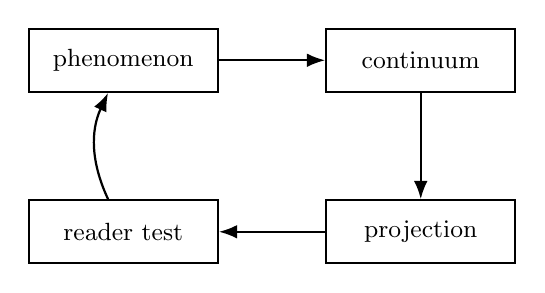
\begin{tikzpicture}[node distance=1.35cm,>=Latex,every node/.style={font=\small}]
\node[draw,thick,align=center,minimum width=2.4cm,minimum height=0.8cm] (a) {phenomenon};
\node[draw,thick,align=center,minimum width=2.4cm,minimum height=0.8cm,right=of a] (b) {continuum};
\node[draw,thick,align=center,minimum width=2.4cm,minimum height=0.8cm,below=of b] (c) {projection};
\node[draw,thick,align=center,minimum width=2.4cm,minimum height=0.8cm,left=of c] (d) {reader test};
\draw[->,thick] (a) -- (b);
\draw[->,thick] (b) -- (c);
\draw[->,thick] (c) -- (d);
\draw[->,thick,bend left=25] (d) to (a);
\end{tikzpicture}
\caption{Mathematical Structuralism Logic Model: concept map of conceptual dependency pressure 14-1-9}
\label{fig:figure-mathematical-structuralism-logic-and-model-theory-one}
\end{figure}
The point of the diagram is not decoration; it marks which relation is being proposed and which stronger conclusion is still unavailable.\par
A local clarification is useful here\par
A local clarification is useful here\footnote{In Mathematical Structuralism Logic Model, this note clarifies the reader clarification role of the term and keeps the caveat close to the sentence that needs it.}.\par
The note keeps the caveat near the term without derailing the main sentence.\par
A structure is an organized pattern of relations. The term is simple, but its consequence is large. If an object is known through its place in a structure, then identity is not only isolated possession. Identity becomes relational position. A point in a geometry, a node in a network, a state in a dynamical system, or a symbol in a formal language can be described by the relations it bears to other positions. This does not make the object unreal. It changes what must be inspected in order to understand it.\par
The move is powerful because many sciences already treat their objects this way. In network science, a highly connected node matters because of its place in a pattern of links. Albert-Laszlo Barabasi and Reka Albert made this vivid in their work on scale-free networks: some networks grow so that a few nodes acquire many more connections than most others, and the resulting structure changes how failure, influence, and spread behave. The importance of a node cannot be read from the node alone. It belongs to the arrangement.\par
The same lesson appears in another form in theoretical ecology. Robert May's work on stability and complexity asked how the stability of an ecosystem changes as the number and strength of interactions grow. A species is not merely an isolated biological unit; it is also a position inside a web of predation, competition, resource use, and mutual dependence. To ask what a species is, in this setting, is also to ask what relations let it persist, change, or disappear.\par
Ontology of Continua, abbreviated here as OC, begins from this need for relational description. OC is a proposed operational metaontology: a vocabulary for describing systems in terms of fields of variation, distinctions, transformations, tensions, and changes of organization. It does not begin by claiming that every domain is secretly the same. It begins from a more modest need: isolated naming is often insufficient. A named thing may still be poorly understood if the conditions of its relation, persistence, and transformation remain unstated.\par
\section{What the Tradition Made Visible In Mathematical Structuralism Logic Model}
Mathematical structuralism has a long ancestry because mathematics has repeatedly found that the same pattern can appear in different clothing. A group may describe rotations of a polygon, permutations of a set, or symmetries of an equation. A graph may describe friendships, roads, citations, neural connections, or dependencies among tasks. The material changes; the pattern can remain. The point is not that material never matters. The point is that some questions become answerable only after the pattern is separated from a particular material instance. \cite{barabasi_scale_free,may_stability_complexity}\par
Logic adds a second discipline to this lineage. A logic is a system for stating valid forms of inference. It tells us how claims may follow from other claims when the rules of implication, quantification, identity, or possibility are fixed. Logic does not by itself decide what exists in the world. It supplies a grammar of consequence. Once a domain has been described in a sufficiently explicit language, logic can ask which statements are entailed, which are inconsistent, and which require assumptions not yet supplied.\par
The local dependency can now be written without changing the claim it supports.\par
\begin{equation}\label{eq:equation-mathematical-structuralism-logic-and-model-theory-two}
\operatorname{massGapToy}_{3} = C_{\mathrm{unres}}=\min_{\pi\in\Pi}\|B(x)-B(\pi x)\|
\end{equation}
The relation names a local dependency, variable dictionary, and proof/evidence role; it is not a claim-status upgrade.\par
The formula is a restraint on the prose. It names the dependency that the surrounding paragraph is allowed to use.\par
The comparison below gives mathematical structuralism logic model a set of quantities that can be inspected instead of merely admired.\par
\begin{table}[htbp]
\centering\small
\caption{Mathematical Structuralism Logic Model: observable quantities and counter-pressure 14-2-9}
\label{tab:table-mathematical-structuralism-logic-and-model-theory-one}
\begin{tabular}{@{}llll@{}}
\toprule
Falsifier & Trigger & Expected failure & Consequence \\
\midrule
mathematical structuralism logic model boundary & 36 units & declared case & fixes what is compared \\
residual pressure & 0.84 & dimensionless & shows unresolved load \\
projection loss & 0.45 & bounded interval & marks lost structure \\
countercase set & 17 cases & review sample & keeps a falsifier visible \\
\bottomrule
\end{tabular}
\end{table}
The table should be read locally: it narrows the comparison without pretending that the wider theory has been settled by a single surface.\par
Model theory adds a third discipline. A model, in this setting, is an interpretation that makes a formal language true in a particular domain. If a language contains symbols for relations, operations, and objects, a model assigns those symbols to a structured domain where sentences can be evaluated. The same formal sentence may have different models. Some models may satisfy a theory; others may not. Model theory therefore separates syntax, the written or symbolic form of a statement, from semantics, the interpretation under which the statement holds.\par
This separation matters for any ambitious vocabulary of systems. A theory can sound precise while leaving its interpretation unstable. A term such as boundary, transformation, contradiction, or emergence may be rhetorically impressive and still fail to identify what changes under observation. Model theory teaches a stricter habit: a formal expression is not yet an explanatory bridge merely because it is formally arranged. One must also know how it is interpreted, what counts as satisfaction, and where the interpretation stops.\par
The lineage from structuralism to logic to model theory therefore supplies a restraint. Structuralism says that positions in systems matter. Logic says that consequence must be governed by explicit rules. Model theory says that formal languages need interpretations and that different interpretations can satisfy the same abstract pattern. Together they prevent a premature leap from elegant vocabulary to empirical reach.\par
A concrete example clarifies the relation. Consider a simple network with nodes and edges. In pure graph theory, the nodes may be abstract positions; only adjacency matters. In a transportation model, nodes may be stations and edges may be rail links. In a neural model, nodes may be units and edges may be weighted influences. The same graph form can appear in each case, but the meaning of a path, a failure, a signal, or a bottleneck changes with the interpretation. Structural sameness does not license semantic sameness.\par
OC inherits this discipline. It can compare domains only if it keeps structural analogy separate from domain identity. A boundary in a cell, a boundary in a legal jurisdiction, and a boundary in a mathematical phase space are not the same object. They may, however, share a role: each separates regimes of behavior, filters interaction, or marks where a rule changes. The disciplined question is not whether they are identical, but whether a shared operational description can be stated without erasing the differences that matter.\par
\section{Where the Inheritance Runs Out In Mathematical Structuralism Logic Model}
The gain from mathematical structuralism is not merely elegance. It gives a way to talk about invariance. An invariant is something that remains stable under a specified transformation. A square may be rotated and still remain a square. A network may be relabeled and still preserve its pattern of connections. A system may change its material occupants while preserving a relation among roles. Invariance allows description to pass beyond surface appearance without pretending that every difference is irrelevant. \cite{barabasi_scale_free,may_stability_complexity}\par
Invariance is central to scientific modeling because systems rarely present themselves twice in exactly the same form. A biological organism grows. A market shifts. A neural state changes with stimulation. An ecological relation intensifies or weakens. If a description depends on every microscopic detail remaining fixed, it becomes useless for comparison. Structural description asks which relations persist across allowed changes and which changes destroy the identity of the pattern under study.\par
The local dependency can now be written without changing the claim it supports.\par
\begin{equation}\label{eq:equation-mathematical-structuralism-logic-and-model-theory-one}
\operatorname{predictionWindow}_{3} = \Delta d=\operatorname{rank}(A_{\mathrm{new}})-\operatorname{rank}(A_{\mathrm{old}})
\end{equation}
The relation names a local dependency, variable dictionary, and proof/evidence role; it is not a claim-status upgrade.\par
The formula is a restraint on the prose. It names the dependency that the surrounding paragraph is allowed to use.\par
The local dependency can now be written without changing the claim it supports.\par
\begin{equation}\label{eq:equation-mathematical-structuralism-logic-and-model-theory-three}
\operatorname{primeDeviationToy}_{3} = P_{\mathrm{collapse}}=\sigma(\alpha R-\beta S-\gamma M)
\end{equation}
The relation names a local dependency, variable dictionary, and proof/evidence role; it is not a claim-status upgrade.\par
The formula is a restraint on the prose. It names the dependency that the surrounding paragraph is allowed to use.\par
A small numerical test keeps the abstraction honest at the scale of a single decision.\par
\paragraph{Numerical example.} For mathematical structuralism logic model, take support=0.53, projection loss=0., and 6 open obligations. The bounded score is 0.; the example gives the reader a numeric scale without pretending to be empirical proof.\par
The numbers are deliberately small; their value is pedagogical, not evidential, unless the chapter binds them to a dataset elsewhere.\par
Alan Turing's work on morphogenesis gives a classic example of structural thinking in a scientific setting. He proposed that interacting chemical processes could generate biological patterns through reaction and diffusion, showing how form might arise from a rule-governed dynamic rather than from a pre-drawn template. The importance of the model lies not in reducing life to chemistry in a simplistic way, but in showing that pattern formation can be studied through relations among processes distributed across space and time.\par
John Hopfield's neural network model offers another example, but it teaches a different lesson. A memory in such a system is not stored as a sentence in one location. It is represented by a stable pattern of activity in a network of interacting units. The memory is structural and dynamic: it belongs to the relations among units and to the tendency of the system to settle into certain states. This makes the example useful because it shows how an object of interest may be neither a single material part nor a vague abstraction, but a constrained pattern in a system.\par
These examples show what a structural model can gain. It can describe distributed causality, where no single component explains the whole. It can describe equivalence across different realizations, where the same organization appears in more than one material setting. It can describe transformation, where the identity of a pattern depends on what changes leave it recognizable. It can also describe failure, because a structure can lose the relations that made it the structure it was.\par
OC uses the word continuum for a domain of variation. A continuum is not simply a smooth line. It may include degrees, thresholds, phases, or relational changes. A city, for example, may vary along a continuum of density, accessibility, cost, risk, or administrative control. These continua are not decorative labels. They identify what can change while the system remains describable.\par
A first-time reader can test the point with the city itself. A city is made of buildings, roads, people, laws, utilities, institutions, and habits. If all residents changed overnight but the legal, infrastructural, and spatial relations remained, one might still call it the same city. If every building remained but the laws, roads, language, and institutions dissolved, the identity would become less clear. The city's being is not exhausted by its matter. It lies in a structured continuity of relations and operations.\par
\section{The Conceptual Debt In Mathematical Structuralism Logic Model}
Structuralism also has a limit, and the limit must be stated plainly. A structure can become too successful in abstraction. Once the pattern is detached from material context, it becomes tempting to treat all instances of the pattern as interchangeable. This is often false. A network of friendships, a network of neurons, and a network of power lines may share graph properties, but the meaning of a link differs sharply. A friendship edge is not a synapse; a synapse is not a cable; a cable is not a legal obligation. \cite{barabasi_scale_free,may_stability_complexity}\par
Model theory helps expose this danger because it distinguishes formal satisfaction from worldly adequacy. A formal structure may satisfy a set of axioms while failing to represent the phenomenon one cares about. A toy model of an ecosystem may be mathematically consistent and still omit seasonal variation, spatial refuges, evolutionary adaptation, or measurement uncertainty. A model of a neural network may exhibit stable states and still fail to capture the biological details of a living brain. Formal success is not the same as empirical reach.\par
A small numerical test keeps the abstraction honest at the scale of a single decision.\par
\paragraph{Numerical example.} For mathematical structuralism logic model, take support=0.56, projection loss=0.12, and 1 open obligations. The bounded score is 0.220; the example gives the reader a numeric scale without pretending to be empirical proof.\par
The numbers are deliberately small; their value is pedagogical, not evidential, unless the chapter binds them to a dataset elsewhere.\par
The case that follows turns the proposal into a sequence of criticizable moves.\par
\paragraph{Worked case.} In the worked case for mathematical structuralism logic model, the claim is reduced to a boundary, an observable, a dependency, a numerical cue, and a falsifier. The case is useful only because each move can be criticized separately.\par
The case helps because each step can fail separately, which is exactly what a useful example should permit.\par
This distinction is essential for OC. Claims about contradiction, emergence, collapse, and projection across domains cannot be carried by structural resemblance alone. If a pattern in one domain resembles a pattern in another, the resemblance must be narrowed: which relations correspond, which operations correspond, what is lost in translation, and what observations would count against the proposed mapping? Without that discipline, structural language becomes a machine for overextension.\par
The objection is direct: if structuralism abstracts from content, does it leave anything real behind? The answer is that abstraction is not deletion when it is governed. A subway map omits building heights, weather, shop names, and street texture. It is still useful because it preserves the relations needed for travel across the rail system. The map becomes misleading only when used for tasks it was not built to answer, such as estimating walking distance through dense streets or judging neighborhood life. The model is real as a model, not as a total replacement for the city.\par
A second objection is that structuralism may smuggle ontology into notation. If one writes a domain in terms of nodes, edges, states, operators, and boundaries, perhaps one has already decided what exists. This concern is serious. The answer cannot be that notation is neutral. Notation selects. It highlights some differences and suppresses others. OC must therefore treat its own terms as controlled instruments rather than final descriptions of reality. A boundary is a proposed operational distinction, not a guarantee that the world has been divided in the only correct way.\par
A third limit concerns identity through change. Structures can transform gradually. At what point is the structure no longer the same? A network can lose nodes and gain nodes. An organism can replace cells. A political institution can revise laws. A scientific field can change its methods. Structuralism supplies tools for tracking invariants, but it does not automatically decide which invariants matter most. That decision depends on the question, the domain, and the cost of error.\par
For this reason, OC cannot use structuralism as a license for universal analogy. It must use it as a discipline of comparison. Its terms have to remain answerable to the domain in which they are applied. A model that compares too little is trivial; a model that compares too much is false. The useful middle is neither decorative abstraction nor captivity to one local case, but controlled translation.\par
\section{The Passage to Continua In Mathematical Structuralism Logic Model}
The limit of structuralism creates a further pressure. Mathematical structuralism can say that objects are positions in structures. Logic can regulate consequence. Model theory can separate language from interpretation. Yet complex systems force additional questions: how do structures change under unresolved tension, how do distinctions arise or fail, how do fields of variation split into new dimensions, and how can a pattern be carried from one domain to another without being inflated into a false identity? \cite{barabasi_scale_free,may_stability_complexity}\par
OC uses the word contradiction in an operational rather than purely logical sense. In ordinary speech, a contradiction is a clash between claims. In formal logic, contradiction has stricter consequences. In OC, the term names a configuration containing incompatible demands, constraints, or tendencies that cannot all be satisfied in the current descriptive frame. This does not mean every tension is logically explosive. It means that some tensions expose a shortage in the available description. The system may find a new dimension of organization, or the configuration may fail to hold together.\par
The distinction can be made concrete. Imagine an ecosystem in which increased connectivity improves resource flow but also amplifies the spread of disturbance. May's analysis of stability and complexity does not say that more complexity is always better or worse; it shows that interaction structure matters for stability. A simple slogan cannot carry the case. The system may require a richer description that separates kinds of connection, strengths of interaction, time scales, and buffering distinctions.\par
The same pattern appears in network growth. Scale-free networks can be robust against random loss of many low-degree nodes while remaining vulnerable to attacks on highly connected hubs. The contradiction is not a formal inconsistency in arithmetic. It is an operational tension: the same organization that supports efficient connectivity can create concentrated vulnerability. A structural description notices the hub pattern; an operational description must ask how the system responds when that pattern becomes a liability.\par
In morphogenesis, too, a system can produce order through instability. Turing's reaction-diffusion model showed how uniformity can give way to pattern under the right dynamics. The important lesson is not that every emergence is a Turing pattern. It is that instability need not be mere failure. Under some conditions, a previous state becomes insufficient, and a new structure appears. The scientific task is to distinguish such cases from collapse, noise, artifact, or overinterpretation.\par
Hopfield networks add another angle. A network may settle into a stable state that functions as memory, but it may also settle into an unwanted state or blur distinct memories if the configuration is overloaded. Stability is therefore not automatically adequacy. A system can resolve into a pattern that is available to its dynamics while still being poor for a particular task. This matters because emergence and collapse cannot be judged only by the presence of order. The order must be interpreted against the system's conditions and use.\par
The pressure on OC is therefore to preserve the gains of structuralism while adding operational discrimination. It must say what varies, what distinction is active, what transformation is occurring, what cannot be jointly satisfied, what new dimension of description is appearing, and what kind of comparison is being licensed. These are controls against two opposite failures: treating every domain as incomparable, or treating every structural resemblance as a result.\par
\section{A Problem Older Than the Vocabulary In Mathematical Structuralism Logic Model structur}
OC can now be stated without theatrical mystery. Ontology of Continua is a proposed operational metaontology: a language for describing systems in terms of continua, boundaries, operators, contradictions, emergence, collapse, hierarchy, and domain projection. The phrase operational metaontology has two parts. Metaontology concerns the kinds of entities, distinctions, and commitments a descriptive scheme permits. Operational means that those commitments must be tied to describable use: what is being distinguished, what changes, what persists, and what would make the description fail. \cite{barabasi_scale_free,may_stability_complexity}\par
This status matters. OC is not presented here as a completed empirical science, a finished formal calculus, or a theorem that automatically governs all systems. It is best understood at this stage as a disciplined heuristic vocabulary and a proto-formal framework: it aims to make certain descriptions more explicit, more comparable, and more vulnerable to correction. Its value depends on whether it narrows claims rather than enlarging them without cost.\par
The bridge from mathematical structuralism to OC is therefore direct but not automatic. Structuralism teaches that objects can be understood by their roles in relational patterns. Logic teaches that inference requires explicit rules. Model theory teaches that formal language must be interpreted in a domain. OC inherits all three lessons and adds a question about transformation: what happens when a system cannot remain adequately described within its current structure?\par
The central hypothesis of OC can be stated cautiously: an unresolved operational contradiction either gives rise to a new dimension of description or contributes to the collapse of the configuration that cannot resolve it. This sentence is not a completed proof and not a universal empirical verdict. It is an organizing hypothesis. Its value at this stage is that it names a recurring problem: systems often fail not because they lack parts, but because their current descriptive axes cannot carry the tensions they generate.\par
A city again provides a plain example. Suppose a growing city treats transport only as road capacity. For a time, that axis may suffice: more vehicles require more lanes. Eventually the same solution worsens congestion, air quality, land use, and social access. The contradiction does not vanish by adding a larger road in the same frame. The city may need a new dimension of description: multimodal mobility, zoning, demand timing, pricing, walkability, or digital coordination. If it cannot generate or adopt such dimensions, parts of the urban configuration may degrade.\par
This example also shows why OC speaks of boundaries. A city boundary may be legal, infrastructural, economic, ecological, or perceptual. Each boundary filters different flows: taxes, traffic, water, labor, pollution, identity. Treating them as one boundary would be crude. Treating them as unrelated would miss their interactions. Boundary language is useful only if it forces the description to say which boundary is active, what it separates, what passes through it, and what changes when it is moved or crossed.\par
Operators enter next. In the city example, an operator may be a zoning rule, a transit schedule, a pricing mechanism, a construction project, or a social practice. Each changes the configuration in a different way. Some operators preserve an existing continuum; others create thresholds or new axes. A congestion charge, for instance, does not merely add a fact to the road system. It changes the relation between movement, cost, time, and access. The system has not just more content, but a different operational geometry.\par
Hierarchy follows because systems are not flat. A household, street, district, city, region, and national infrastructure can all participate in the same transport problem. A local intervention may solve one scale while worsening another. Structuralism gives relations; OC asks how relations are arranged across levels and how a contradiction at one level may be absorbed, displaced, amplified, or transformed at another. The language of continua becomes more than a metaphor when it requires variation to be tracked across scale and regime.\par
Domain projection is the most dangerous and most necessary bridge. A domain projection occurs when a descriptive pattern from one domain is mapped into another domain under explicit limits. Network robustness, ecological stability, morphogenetic patterning, and neural attractors may illuminate OC's vocabulary, but none of them can be copied wholesale into ontology. Barabasi helps with network structure, May with interaction and stability, Turing with pattern formation, and Hopfield with distributed stable states. Their contributions remain distinct.\par
The discipline of status is therefore part of the argument. OC has been positioned as a proposed language and organizing hypothesis, not as an established law of nature. A formal vocabulary alone does not supply data. A suggestive analogy alone does not prove a projection. A system may be described in OC terms and still be described badly. The test is whether the vocabulary makes the description more exact: what varies, what separates, what transforms, what fails, and what would count as correction.\par
The objection that remains is whether OC adds anything beyond familiar systems language. The answer depends on whether its terms make descriptions narrower and more inspectable. If continuum, boundary, operator, contradiction, emergence, collapse, hierarchy, and projection merely rename ordinary complexity, then OC fails as a useful language. If they force a description to specify the active variation, the operative distinction, the transforming rule, the unsatisfied demand, the appearing axis, the failed configuration, the relevant level, and the licensed mapping, then the language earns a role.\par
Mathematical structuralism, logic, and model theory do not complete OC. They teach it how to behave. From structuralism it learns that being can be relational without becoming unreal. From logic it learns that consequence needs rules. From model theory it learns that language and interpretation must not be confused. From scientific modeling it learns that abstraction is powerful only when its limits are known. The result is not a final ontology, but a disciplined opening: a way to ask how entities persist, transform, and fail within the structures that make them intelligible.\par
\chapter{General Systems Theory, Cybernetics, and Operational Description}
\section{A Problem Older Than the Vocabulary In General Systems Theory Cybernetics}
A system is not first encountered as a theorem. It is encountered as something that keeps changing while still seeming to remain itself. A pond warms through the afternoon, cools under evening air, receives rain, grows algae near the shallows, loses oxygen under ice, gathers silt at the inlet, and still remains one pond. Its surface can look calm while chemical gradients, larvae, roots, bacteria, light, and temperature are altering the conditions of life below. To call it one thing is already to make a descriptive decision. To understand it, one has to say how the thing keeps enough continuity across change to be recognized at all. \cite{may_stability_complexity,turing_morphogenesis}\par
The same difficulty appears in less visible forms. A nervous system learns a pattern, loses another, compensates after injury, and remains one organismic process. A city changes laws, prices, traffic, neighborhoods, habits of speech, and methods of administration while still being named as one city. A family, a laboratory, a language, and a forest each persist through alteration, but not in the same way. The first difficulty is not whether such things exist. The difficulty is how to describe their being without freezing them into objects too simple for their behavior.\par
The next diagram slows the argument down just enough to show how general systems theory cybernetics is being organized.\par
\begin{figure}[htbp]
\centering
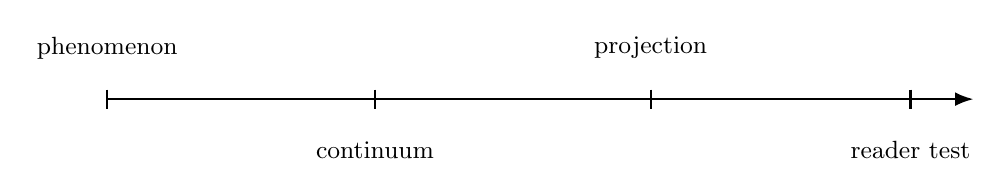
\begin{tikzpicture}[node distance=1.35cm,>=Latex,every node/.style={font=\small}]
\draw[->,thick] (0,0) -- (11,0);
\node[align=center] at (0,0.65) {phenomenon};
\node[align=center] at (3.4,-0.65) {continuum};
\node[align=center] at (6.9,0.65) {projection};
\node[align=center] at (10.2,-0.65) {reader test};
\foreach \x in {0,3.4,6.9,10.2} \draw[thick] (\x,0.12) -- (\x,-0.12);
\end{tikzpicture}
\caption{General Systems Theory Cybernetics: historical timeline of conceptual dependency pressure 15-1-10}
\label{fig:figure-general-systems-theory-cybernetics-and-operational-descr-one}
\end{figure}
The point of the diagram is not decoration; it marks which relation is being proposed and which stronger conclusion is still unavailable.\par
A local clarification is useful here\par
A local clarification is useful here\footnote{In General Systems Theory Cybernetics, this note clarifies the reader clarification role of the term and keeps the caveat close to the sentence that needs it.}.\par
The note keeps the caveat near the term without derailing the main sentence.\par
General Systems Theory and cybernetics entered modern thought at this pressure point. They did not begin by asking only what a thing is made of. They asked how a whole maintains organization, how parts constrain one another, how signals circulate, how feedback alters future behavior, and how the same descriptive pattern may appear, with important differences, in machines, organisms, ecologies, and societies. This changed the question of being. A thing could no longer be described adequately by listing its components. Its organization, boundary, exchange, regulation, and history also mattered.\par
Consider a thermostat in a cold room. The device is simple enough to be misleading, but that is also why it teaches clearly. The air cools. The sensor registers a temperature below a chosen range. A comparison is made against a set point. The heater switches on. Warm air begins to move through the room, first unevenly, then more generally. The sensor later registers the changed condition and the heater switches off. Even here, the object of description is not only the small box on the wall. It is a loop: sensor, comparison, actuator, room, heat flow, delay, and renewed measurement. Remove the loop and the remaining parts no longer explain the behavior.\par
The same lesson becomes less tidy in biological cases. A population of insects, a developing embryo, a neural circuit, or a forest is not controlled by a single visible lever. There are local interactions, constraints, delays, thresholds, and amplifications. The pattern may hold for a time, then drift, reorganize, or collapse. If being is described only as substance, these changes appear secondary. If being is described operationally, the persistence of the system depends on the continuing work by which its parts and surroundings maintain a recognizable configuration.\par
An operational description is a description in terms of acts, relations, measurements, transformations, and repeatable distinctions. It does not merely name a thing. It specifies what is being distinguished, what changes are being tracked, what counts as the boundary of the case, and what operations connect one condition to another. This is not a reduction of being to machinery. It is a way of speaking carefully about systems that do not sit still long enough to be understood by static classification alone.\par
\section{What the Tradition Made Visible In General Systems Theory Cybernetics}
General Systems Theory gave modern science one of its strongest formulations of a whole as more than an inventory of parts. Its central intuition was not mystical. It was descriptive. Many domains contained organized complexes whose behavior depended on relations among components as much as on the components considered separately. A cell, a market, a machine, and an ecosystem cannot be made intelligible by naming their pieces in isolation. The arrangement and exchange among those pieces matter. \cite{may_stability_complexity,turing_morphogenesis}\par
Cybernetics sharpened this intuition by focusing on control and communication. A cybernetic system is one in which information about the state of a process can alter the future course of that process. Feedback is the central term. Negative feedback reduces deviation, as in the thermostat that corrects temperature. Positive feedback amplifies deviation, as when an initial advantage in a population, market, or signal chain becomes self-reinforcing. Feedback made it possible to describe stability and instability as active achievements, not as mere properties of inert things.\par
The local dependency can now be written without changing the claim it supports.\par
\begin{equation}\label{eq:equation-general-systems-theory-cybernetics-and-operational-descr-two}
\operatorname{regularityResidual}_{3} = \tau_{\mathrm{repair}}=\inf\{t:C(t)<\theta\}
\end{equation}
The relation names a local dependency, variable dictionary, and proof/evidence role; it is not a claim-status upgrade.\par
The formula is a restraint on the prose. It names the dependency that the surrounding paragraph is allowed to use.\par
The comparison below gives general systems theory cybernetics a set of quantities that can be inspected instead of merely admired.\par
\begin{table}[htbp]
\centering\small
\caption{General Systems Theory Cybernetics: observable quantities and counter-pressure 15-2-10}
\label{tab:table-general-systems-theory-cybernetics-and-operational-descr-one}
\begin{tabular}{@{}llll@{}}
\toprule
Level & Axis pressure & Operator burden & Transition test \\
\midrule
general systems theory cybernetics boundary & 39 units & declared case & fixes what is compared \\
residual pressure & 0.00 & dimensionless & shows unresolved load \\
projection loss & 0.56 & bounded interval & marks lost structure \\
countercase set & 18 cases & review sample & keeps a falsifier visible \\
\bottomrule
\end{tabular}
\end{table}
The table should be read locally: it narrows the comparison without pretending that the wider theory has been settled by a single surface.\par
The importance of this move is visible in developmental biology. Alan Turing's work on morphogenesis proposed that simple chemical interactions could generate patterned form under suitable conditions. The point was not that every biological pattern had thereby been explained. The point was that form could be approached as the outcome of rule-governed processes distributed through a medium, not only as the execution of a pre-drawn blueprint. In that sense, Turing's morphogenesis work belongs to the history of operational description: it treats form as something produced through interaction over time.\par
A related lesson appears in studies of ecological stability. Robert May's work on stability and complexity challenged the comforting assumption that more complex ecological networks are automatically more stable. The value of May's stability-complexity result is not a license to generalize from one mathematical ecology setting to every organized whole. It is a warning. A network's behavior depends on the pattern and strength of relations, not merely on the number of parts. Complexity is not an honorific. It can stabilize, destabilize, buffer, delay, or conceal failure depending on the structure under description.\par
Neural theory provides another line. Donald Hebb introduced a principle of learning in which repeated co-activity among neural elements changes their future relation. The familiar phrase used to summarize this idea is simpler than the theory itself, but Hebbian learning marks an important conceptual turn: organization can be modified by activity. Later, Hopfield networks showed how recurrent neural systems could settle into stable patterns that function like attractors. In such networks, memory is not a stored inscription sitting in one place. It is a dynamic pattern available to the network under certain conditions.\par
These examples do not prove a single universal ontology of systems. They show something more modest and more useful. They show why modern scientific description became increasingly uncomfortable with treating being as a static inventory. Systems have states, but they also have transitions. They have parts, but also couplings. They have boundaries, but those boundaries may regulate exchange rather than simply separate inside from outside. They may persist, but persistence may depend on continuous operations that can fail.\par
\section{Where the Inheritance Runs Out In General Systems Theory Cybernetics}
The gain from General Systems Theory and cybernetics is a new kind of object for thought: the organized process. An organized process is neither a heap nor a timeless essence. It is a configuration whose identity depends on patterned relations across change. This does not abolish ordinary objects. It refines the description of cases in which ordinary object language becomes too blunt. A heart is an organ, but its systemic significance lies in circulation, rhythm, pressure, oxygen transport, nervous regulation, and failure modes. The noun is useful; the process explains why the noun matters. \cite{may_stability_complexity,turing_morphogenesis}\par
This gain can be stated through the idea of state. A state is a describable condition of a system at a time or under a specified observational cut. In a room, the temperature, heater status, insulation, and air movement can form part of a state description. In a neural network, activation levels and connection strengths may form part of a state description. In an ecosystem, population sizes, resource flows, seasonal constraints, and interaction strengths may form part of a state description. A state is not the whole being of a system, but it gives description a handle.\par
The local dependency can now be written without changing the claim it supports.\par
\begin{equation}\label{eq:equation-general-systems-theory-cybernetics-and-operational-descr-one}
\operatorname{complexityVerifier}_{3} = \operatorname{loss}_{\phi}=1-\frac{|E_{\phi}\cap E_{\mathrm{domain}}|}{|E_{\mathrm{domain}}|}
\end{equation}
The relation names a local dependency, variable dictionary, and proof/evidence role; it is not a claim-status upgrade.\par
The formula is a restraint on the prose. It names the dependency that the surrounding paragraph is allowed to use.\par
The local dependency can now be written without changing the claim it supports.\par
\begin{equation}\label{eq:equation-general-systems-theory-cybernetics-and-operational-descr-three}
\operatorname{rankGrowthToy}_{3} = I_{\mathrm{axis}}=\frac{\operatorname{Var}(x\mid a)}{\operatorname{Var}(x)}
\end{equation}
The relation names a local dependency, variable dictionary, and proof/evidence role; it is not a claim-status upgrade.\par
The formula is a restraint on the prose. It names the dependency that the surrounding paragraph is allowed to use.\par
A small numerical test keeps the abstraction honest at the scale of a single decision.\par
\paragraph{Numerical example.} For general systems theory cybernetics, take support=0.59, projection loss=0.17, and 2 open obligations. The bounded score is 0.140; the example gives the reader a numeric scale without pretending to be empirical proof.\par
The numbers are deliberately small; their value is pedagogical, not evidential, unless the chapter binds them to a dataset elsewhere.\par
Once states can be described, transitions can be described. A transition is a movement from one state or state range to another under some operation, interaction, or condition. The thermostat does not merely have the state cold and the state warm. It moves between them through sensing, switching, heating, delay, and renewed sensing. A population does not merely have abundance and scarcity. It moves through reproduction, predation, disease, migration, and environmental constraint. Operational description asks what makes such transitions possible, probable, reversible, or terminal.\par
Feedback then gives transition a structure. Negative feedback can preserve a range. Positive feedback can drive a change beyond a former range. Delayed feedback can cause oscillation. Weak feedback may fail to correct drift. Overcorrection may destabilize what it tries to regulate. These patterns are not metaphors when the operations are specified. They become ways of saying what is being measured, how the system responds, what time scale matters, and where the response changes the conditions of the next response.\par
The model also gains a clearer account of boundary. A boundary is not only a line around an object. In systems description, a boundary is the distinction that determines which relations are counted as internal to the described system and which are treated as environment, input, output, disturbance, or condition. The skin of an organism is one kind of boundary. A membrane is another. A legal jurisdiction, a computational interface, a species range, a laboratory vessel, and a measurement protocol can also function as boundaries. The boundary is part of the description because changing it can change what the system is taken to be.\par
This matters because many false arguments about systems come from unstable boundaries. One speaker treats a city as a legal municipality. Another treats it as a labor market. Another treats it as a transportation network. Another treats it as a cultural memory. Each may be describing something real, but not the same system under the same boundary. Operational description does not solve this by choosing one boundary for all purposes. It requires the boundary to be declared clearly enough that claims can be understood, compared, and challenged.\par
The model gained from systems and cybernetics is therefore not a doctrine that everything is one system. It is a method for preventing several common confusions. It distinguishes component from relation, state from transition, stability from stasis, boundary from mere outline, and regulation from command. It lets one ask whether a whole persists because its parts are fixed or because its operations continually reproduce an organized range. The question is historical as much as theoretical: modern thought needed a language for organized change, and systems theory gave it one.\par
\section{The Conceptual Debt In General Systems Theory Cybernetics}
The systems and cybernetic inheritance is powerful, but it is not enough. Its first danger appears when description becomes too general. Saying that a poem, an embryo, a market, and a climate are all systems may be true at a high level, but it is not yet informative. The word system can become a container into which every difficult object is placed. When that happens, the language stops distinguishing. It names interdependence without specifying the kind of interdependence, the relevant boundary, the operations at work, or the criteria by which a claim could fail. \cite{may_stability_complexity,turing_morphogenesis}\par
Analogy is the next danger, precisely because cybernetic language travels so easily. Feedback, signal, control, input, output, noise, and regulation can illuminate many domains. They can also mislead. A political community is not a thermostat. A developing organism is not a simple servomechanism. A neural network is not a parliament. Analogies become legitimate only when the operations named by the analogy can be identified in the target case. Otherwise, the language creates a false sense of explanation.\par
A small numerical test keeps the abstraction honest at the scale of a single decision.\par
\paragraph{Numerical example.} For general systems theory cybernetics, take support=0.42, projection loss=0.10, and 3 open obligations. The bounded score is 0.; the example gives the reader a numeric scale without pretending to be empirical proof.\par
The numbers are deliberately small; their value is pedagogical, not evidential, unless the chapter binds them to a dataset elsewhere.\par
The case that follows turns the proposal into a sequence of criticizable moves.\par
\paragraph{Worked case.} In the worked case for general systems theory cybernetics, the claim is reduced to a boundary, an observable, a dependency, a numerical cue, and a falsifier. The case is useful only because each move can be criticized separately.\par
The case helps because each step can fail separately, which is exactly what a useful example should permit.\par
The thermostat example shows both the strength and the danger. It teaches feedback clearly because the loop is simple. But the clarity comes from artificial narrowing. The device has an engineered set point, a designed sensor, a specified actuator, and a limited range of relevant variation. Many natural and social systems do not have a single set point. They may contain competing regulatory processes, shifting thresholds, multiple scales, and agents that change their own interpretation of the system. Carrying the thermostat image too far turns an instructive case into a distortion.\par
A concrete failure can be seen when public opinion is treated as if it were room temperature. Polling may measure something real, but a population does not merely register a deviation and return to equilibrium. The act of measurement can enter public discussion. Reported results may change expectations, funding, turnout, fear, imitation, or resignation. The same number can mean different things under different electoral rules, media conditions, and social pressures. To describe this as feedback may help only if the channels, delays, incentives, and interpretive effects are made explicit. Without that work, the analogy borrows mechanical clarity while losing the phenomenon.\par
Another failure appears when biological language is imported into markets without restraint. A company may be called an organism, an industry an ecosystem, and competition a form of selection. Some comparisons can be useful. Others smuggle in assumptions that do not hold. Firms can plan, lobby, merge, change rules, and represent themselves symbolically in ways that organisms in an ecological model do not. Bankruptcy is not death in the biological sense; assets, debts, skills, brands, and contracts may be reorganized. Here again, systems language helps only when it is reformulated for the domain instead of carried over whole.\par
Observation introduces its own limit. Systems are often described from outside, as if the observer can define the boundary, list the variables, and track the transitions without altering the case. In many scientific contexts that is a reasonable approximation. In others, especially in social, cognitive, and experimental settings, the act of observing, measuring, modeling, or intervening may enter the system's subsequent behavior. Operational description has to remain honest about the observational cut. It has to ask not only what is described, but how the description obtains its object.\par
Emergence brings a final temptation. Emergence names the appearance of properties, patterns, or behaviors at one level that are not straightforwardly visible in the parts taken separately. The term is useful because many organized wholes do display patterns that cannot be read off from isolated components. It is dangerous because it can become a decorative label placed where explanation has stopped. Systems theory made emergence respectable as a problem of organized wholes. It did not by itself provide a complete grammar for deciding when an emergent claim is strong, weak, speculative, operationally defined, or merely suggestive.\par
This is why caution about scientific standing matters. A proposed systems description can be suggestive without being established. A model can be mathematically clean while applying only to an idealized class. A simulation can show behavior within assumptions without demonstrating that a natural system behaves the same way. A comparison can be illuminating without being decisive. A formal proof can secure a statement inside a formal setting without settling whether the setting captures the empirical case. The inheritance from systems and cybernetics must be used without inflating what each method has actually shown.\par
The limitation can be put sharply: General Systems Theory and cybernetics taught modern thought how to describe organized processes, but they did not fully settle how to compare descriptions across domains without erasing domain differences. The same words can travel farther than their warrants. Feedback in an engineered controller, a neural circuit, an ecosystem, and a culture may share a family resemblance, but each requires its own observables, timescales, and failure criteria. The strength of systems language is its mobility. Its weakness is that mobility can become carelessness.\par
\section{The Passage to Continua In General Systems Theory Cybernetics}
A useful model often creates demands it cannot satisfy on its own. The systems and cybernetic model did exactly this. It made relations, feedback, boundary, state, and transition central. Once those terms became available, they began to move across fields with great force. Sometimes they clarified. Sometimes they blurred. The problem was not that they traveled, but that their travel needed discipline. Without such discipline, one gets either fragmentation or overreach. Fragmentation leaves every domain with its own private vocabulary. Overreach declares the same pattern everywhere and loses the specificity that made the pattern meaningful. \cite{may_stability_complexity,turing_morphogenesis}\par
The pressure is visible in the question of levels. A neural network can be described at the level of individual units, activation patterns, learned attractors, task behavior, organismic function, or social use. An ecosystem can be described at the level of organisms, populations, trophic relations, nutrient cycles, climate coupling, or human management. No single level automatically invalidates the others. Yet claims made at one level cannot simply be transferred to another. They must be carried carefully, with attention to what is preserved, what is lost, and what changes meaning during the movement.\par
This need for careful movement becomes especially clear when descriptions use graded ranges rather than simple oppositions. Temperature, pressure, density, excitation, dependency, integration, and organizational coupling can often be treated as ranges when the domain permits it. Such ranges do not mean vagueness. They mean that the relevant distinction may require degrees rather than a yes or no. Many systems do not change by flipping instantly from one kind to another. They drift, intensify, weaken, bifurcate, saturate, and sometimes fail.\par
But graded language also creates risk. If every difference is softened into a range, distinctions lose force. A description must therefore say which range is being used, what its observable anchors are, and how movement within it is identified. In a thermal system, temperature has well-established measurement practices. In a social system, dependency or legitimacy may require more careful construction and may remain more contestable. The point is not to pretend that all domains have equal maturity of measurement. The point is to keep each claim tied to the methods by which it can be known.\par
There is also a pressure that arises from conflict within organization. In ordinary speech, a contradiction is a clash between claims. In systems description, the more relevant case is often a clash between operational demands that cannot both be satisfied under the current arrangement. A growing population may require more resources than its environment can supply. A learning system may need plasticity to adapt and stability to preserve past learning. A social institution may need openness to new information and closure to maintain identity. The conflict is not merely verbal. It is a pressure within the configuration.\par
Such pressures do not all end the same way. A system may absorb them by adjustment. It may displace them into another part of the organization. It may require a new description because the old variables no longer explain the case. Or it may lose the organization by which it had remained the same kind of thing. These distinctions are modest, but they matter. Without them, words such as emergence, stability, crisis, and collapse become too blunt. They point toward change without saying what kind of change is at stake.\par
The history of systems and cybernetics therefore does not merely sit behind contemporary theory as ancestry. It leaves a problem still alive. How can one speak across domains without flattening them? How can one describe boundary, state, transition, feedback, and emergence while keeping observables local to the domain? How can one compare a neural attractor, ecological stability, developmental patterning, and social organization without pretending that they are the same object? Any broader ontology of systems must begin by accepting the force of those questions.\par
\section{A Problem Older Than the Vocabulary In General Systems Theory Cybernetics cybernet}
The Ontology of Continua, abbreviated OC, enters at this point as an attempt to make cross-domain systems language more exact. An ontology says what kinds of things a description treats as real or admissible. A metaontology examines and organizes the ways such ontologies are built, compared, and constrained. OC is operational because it asks descriptions to specify boundaries, ranges, transformations, levels, and rules of transfer rather than relying on broad resemblance alone. Its ambition is not to replace domain science. It is to provide a disciplined language for comparing system descriptions while preserving the fact that different domains have different observables. \cite{may_stability_complexity,turing_morphogenesis}\par
The first bridge from systems theory to OC is the boundary. Systems theory made boundary indispensable, but often left boundary choice dependent on the modeler's convenience. OC treats boundary selection as a central act of description. A boundary determines what counts as internal relation, external condition, input, output, disturbance, or neighboring system. This does not make boundaries arbitrary. It makes their function inspectable. A claim about a cell, a market, or a neural network changes when the boundary changes. OC keeps that change visible.\par
The second bridge is the continuum. Systems and cybernetics often described variables, ranges, thresholds, and dynamics, but did not always give a general vocabulary for how such ranges function across domains. OC uses continua to mark structured ranges of variation. A continuum may be quantitative, qualitative with ordered anchors, or formally defined inside a model. Its standing depends on the domain and the available methods. The same restraint applies throughout: do not treat a loose metaphor as a measured axis, and do not treat a measured variable as if it automatically carries the same meaning in another domain.\par
The third bridge is the operator. An operator is a specified transformation that moves, constrains, maps, combines, or reorganizes a described configuration. Heating a room, inhibiting a neural unit, changing a coupling strength, narrowing a legal definition, or moving a model from one level to another can all be operator-like only if the transformation is stated clearly. OC needs the operator concept because systems do not merely have properties. They undergo transformations, and the description must say what kind of transformation is being claimed.\par
The fourth bridge is hierarchy. A hierarchy is an ordered relation among levels of description, not necessarily a command structure. Cells, tissues, organs, organisms, populations, and ecosystems can form one biological hierarchy. Units, layers, network states, tasks, and behavior can form another kind of hierarchy in computational or neural settings. OC treats hierarchy as a descriptive relation that must be specified rather than assumed. A higher-level pattern may depend on lower-level activity without being easily restated as a list of lower-level parts.\par
The fifth bridge is projection, the controlled translation of a description from one boundary, level, domain, or formal setting into another. It is controlled because something is always lost, added, idealized, or reweighted. The lesson from systems history is that concepts travel. The discipline added by OC is that travel has to be named. Feedback in an engineered device, recurrent neural activity, ecological interaction, and institutional response may be compared only after the relevant operations, observables, and limits of the comparison have been made explicit.\par
OC's central hypothesis can now be heard in the right register: an unresolved operational conflict either gives rise to a new dimension of description or breaks the configuration that cannot resolve it. This is not a theorem about every system. It is an organizing hypothesis about organized configurations under pressure. It belongs after systems and cybernetics because it concerns boundary, transformation, maintenance, and failure across change. It also inherits their burden: each stronger claim must be earned through definition, argument, formal treatment where possible, and domain-specific application.\par
The bridge also clarifies what OC does not get to claim merely by inheritance. It does not inherit proof from cybernetics. It does not inherit empirical confirmation from Turing's work on morphogenesis, May's ecological models, Hebbian learning, or Hopfield networks. Those works show that operational, relational, and dynamic descriptions have been scientifically fruitful in particular ways. They do not validate every future use of systems language. OC must still earn its claims one by one.\par
The closing lesson is therefore precise. General Systems Theory and cybernetics supplied modern thought with a language for organized, bounded, dynamic, relational being. They also revealed the danger of a language that moves too easily. OC begins from both facts. It keeps the systems insight that persistence is often operational, and it adds the demand that continua, operators, boundaries, contradictions, and projections be stated with enough care that comparison does not become equivalence. A system is not less real because it changes. It becomes intelligible only when the change by which it remains, fails, or transforms can be described.\par
\chapter{Complexity, Process Ontology, and Dynamical Systems}
\section{A Problem Older Than the Vocabulary In Complexity Process Ontology Dynamical}
A whirlpool is made of water, but it is not identical with any parcel of water. A candle flame is made possible by wax, oxygen, heat, and vapor, but no one of these is the flame. A wound is tissue damage, immune response, clotting, repair, pain, risk, and time. A memory depends on cells and synapses, yet the remembered pattern is not a small object hidden in one cell. A court is carried by people, buildings, records, procedures, habits of obedience, and recognized authority, but it can outlast any judge. In each case, the thing is real. The difficulty is that its reality is not exhausted by listing its parts. \cite{turing_morphogenesis,hopfield_nn}\par
The familiar habit of thought begins with objects. It asks what a thing is, what properties it has, and where it is located. This habit is indispensable. Stones, tools, bones, chairs, documents, and bodies need names, boundaries, and descriptions. Yet many of the entities that matter most are not inert occupants of space. They persist by doing something. They hold together through exchange, regulation, repetition, repair, interpretation, or constraint. Their being is not a static possession behind their activity. Their being is organized activity sustained long enough to be recognized, affected, and sometimes destroyed.\par
The next diagram slows the argument down just enough to show how complexity process ontology dynamical is being organized.\par
\begin{figure}[htbp]
\centering
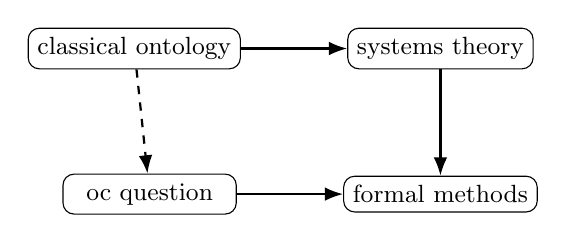
\begin{tikzpicture}[node distance=1.35cm,>=Latex,every node/.style={font=\small}]
\node[draw,rounded corners,align=center,minimum width=2.2cm] (a) {classical ontology};
\node[draw,rounded corners,align=center,minimum width=2.2cm,right=of a] (b) {systems theory};
\node[draw,rounded corners,align=center,minimum width=2.2cm,below=of b] (c) {formal methods};
\node[draw,rounded corners,align=center,minimum width=2.2cm,left=of c] (d) {oc question};
\draw[->,thick] (a) -- (b);
\draw[->,thick] (b) -- (c);
\draw[->,thick] (d) -- (c);
\draw[->,thick,dashed] (a) -- (d);
\end{tikzpicture}
\caption{Complexity Process Ontology Dynamical: dependency dag of historical sequence pressure 16-1-11}
\label{fig:figure-complexity-process-ontology-and-dynamical-systems-one}
\end{figure}
The point of the diagram is not decoration; it marks which relation is being proposed and which stronger conclusion is still unavailable.\par
A local clarification is useful here\par
A local clarification is useful here\footnote{In Complexity Process Ontology Dynamical, this note clarifies the reader clarification role of the term and keeps the caveat close to the sentence that needs it.}.\par
The note keeps the caveat near the term without derailing the main sentence.\par
A process is an ordered transformation through which a pattern is maintained, altered, or lost. It is not merely one event following another. The boiling of water, the healing of skin, the learning of a skill, the growth of a city, and the collapse of trust all involve temporal order, but each has a different structure. In a process, earlier states shape later ones. Conditions matter. Thresholds matter. Interruption matters. A process can succeed, stall, reverse, or fail. To call something a process is therefore not to make it vague. It is to ask what transformation is occurring and what pattern is at stake.\par
The candle flame gives the point in miniature. It has a visible shape and can be pointed to, but it survives only through continuous replacement. Fuel rises, oxygen enters, molecules react, heat circulates, light appears, and the form sustains itself by consuming what supports it. Remove the oxygen, and the flame vanishes. Scatter the heat too quickly, and it dies. The flame is not less real because it is processual. It is real in the way a maintained transformation is real. Its stability is dynamic, not inert.\par
A system is a bounded pattern of relations treated as a unit for inquiry. The boundary may be material, as with a cell membrane; functional, as with the operating range of a thermostat; observational, as with the region selected for a weather model; or institutional, as with a court, school, or central bank. A system is not necessarily sealed. Most significant systems exchange matter, energy, information, force, permission, or constraint with their surroundings. The boundary matters because it tells us what is being treated as internal, what is being treated as external, and what kinds of passage between the two are possible.\par
Complex systems unsettle any theory of being that begins and ends with separable objects. In a complex system, many parts interact so that the future state depends on relations among parts, not merely on the parts taken one by one. The same elements can participate in different organizations under different constraints. Water molecules can be cloud, snowflake, river, blood plasma, or steam. Neurons can support perception, action, memory, expectation, fear, and decision depending on their organization and activity. People in a crowd, a jury, a market, a laboratory, and a family remain biological persons, yet the collective patterns differ because the relations differ.\par
The wound on skin shows why no single level of description is enough. At one level there are cells moving, dividing, signaling, and dying. At another there are clotting, inflammation, immune surveillance, tissue rebuilding, and scar formation. At another there is the organism protecting mobility, sensation, and survival. At still another there may be social meanings: care, work interruption, disability, risk, or stigma. None of these descriptions abolishes the others. The wound is not only chemistry, not only tissue mechanics, not only immune response, not only pain, and not only practical consequence. It is a site where several lawful descriptions meet.\par
This does not mean that everything melts into flux. The skin has a boundary. The wound has an extent. The organism can heal or fail to heal. The scar may remain. Processes have edges, durations, thresholds, and outcomes. A theory that treats every entity as a static object misdescribes maintained organizations. A theory that treats everything as undifferentiated becoming also fails, because storms dissipate, cells die, institutions collapse, memories disappear, and habits can be broken. The task is to think stability and transformation together.\par
Complexity is not a decorative word for difficulty. It names organized behavior arising from interacting elements, often involving feedback, nonlinearity, and scale. Feedback occurs when the result of a process returns to influence the process that produced it. Nonlinearity occurs when a small change in one condition can produce a large difference in outcome, while a large change elsewhere may produce little visible effect. Scale matters because a pattern visible at one level may be absent, misleading, or irrelevant at another. These ideas do not replace ordinary description. They discipline it where ordinary object language becomes too thin.\par
The object-first habit is not simply wrong. It is incomplete. A book is an object, but a legal code is not only paper and ink. A brain is an organ, but a thought is not simply a lump inside it. A city has roads and buildings, but traffic is not reducible to asphalt, engines, and pedestrians considered separately. The question is not whether objects exist. They do. The deeper question is what kinds of existence belong to organized patterns that persist only through ongoing activity. Complexity forces that question into the open.\par
\section{What the Tradition Made Visible In Complexity Process Ontology Dynamical}
The modern language of complexity did not appear as a single doctrine. It grew from several scientific pressures that made older habits of explanation insufficient. Mathematics, biology, physics, cybernetics, computation, and neuroscience all encountered phenomena that could not be understood by isolating a smallest part and assigning the reality of the whole to that part. Reduction remained powerful where decomposition preserved the phenomenon. It became misleading where decomposition destroyed the very organization one hoped to explain. \cite{turing_morphogenesis,hopfield_nn}\par
One of the clearest historical cases came from the problem of biological form. For a long time, the appearance of organized shape in living bodies invited two unsatisfying temptations. One was to imagine a hidden blueprint already containing the finished form in miniature. The other was to treat form as an external plan imposed on passive matter. Developmental biology needed a different kind of language: one in which form could arise through lawful interaction without being pre-drawn at every point.\par
The local dependency can now be written without changing the claim it supports.\par
\begin{equation}\label{eq:equation-complexity-process-ontology-and-dynamical-systems-two}
\operatorname{institutionalLatency}_{3} = \rho_{\mathrm{replay}}=\frac{N_{\mathrm{matched}}}{N_{\mathrm{declared}}}
\end{equation}
The relation names a local dependency, variable dictionary, and proof/evidence role; it is not a claim-status upgrade.\par
The formula is a restraint on the prose. It names the dependency that the surrounding paragraph is allowed to use.\par
The comparison below gives complexity process ontology dynamical a set of quantities that can be inspected instead of merely admired.\par
\begin{table}[htbp]
\centering\small
\caption{Complexity Process Ontology Dynamical: observable quantities and counter-pressure 16-2-11}
\label{tab:table-complexity-process-ontology-and-dynamical-systems-one}
\begin{tabular}{@{}llll@{}}
\toprule
Example & Parameter & Value & What changes \\
\midrule
complexity process ontology dynamical boundary & 42 units & declared case & fixes what is compared \\
residual pressure & 0. & dimensionless & shows unresolved load \\
projection loss & 0.67 & bounded interval & marks lost structure \\
countercase set & 19 cases & review sample & keeps a falsifier visible \\
\bottomrule
\end{tabular}
\end{table}
The table should be read locally: it narrows the comparison without pretending that the wider theory has been settled by a single surface.\par
Alan Turing, remembered chiefly for computation, entered this problem through morphogenesis, the generation of form. In his work on chemical pattern formation, he showed how interacting substances spreading at different rates could produce organized spatial patterns. The point was not that one equation explained all development. It did not then and does not now. The point was that form could be modeled as an outcome of dynamic relations. Pattern did not have to be a separate substance laid over matter. It could arise from reaction, diffusion, rate, instability, and constraint.\par
Imagine a field of developing tissue in which one chemical influence locally encourages a change while another suppresses it over a broader range. Neither influence by itself contains a stripe, spot, or segment. Yet the relation between their rates and ranges can make a patterned distribution appear. The form is not painted on from outside. It is generated through the system's own dynamics. This changed the ontological grammar of the problem. The pattern is real, but its reality is neither that of a miniature preformed object nor that of a ghostly plan. It is a stable result of organized transformation.\par
The historical importance of this shift is larger than the specific model. It showed that one could speak rigorously about the birth of form without treating form as either illusion or substance. A stripe on an animal, a branching structure, or a repeated biological motif could be approached as the result of processes interacting under constraints. In such cases, the question changes from what object is hidden behind the appearance to what dynamics generate and maintain the appearance. Scientific practice had to adopt verbs as seriously as nouns.\par
A second lineage came from learning and neural organization. Donald Hebb proposed that connections among neural units could strengthen through patterns of co-activity. The familiar summary is often compressed into a slogan, but the philosophical importance lies in the relational shift. Learning becomes a change in the organization of a system because of its own history of activity. A memory is not a complete inscription stored in one privileged place. It is a changed disposition of a network to respond, complete, anticipate, or recognize.\par
This makes persistence relational. If a person learns to recognize a melody, the melody is not stored as a tiny inner performance. Recognition depends on a system altered by prior encounters. The pattern may be evoked by a few notes, confused with a similar tune, strengthened through repetition, or lost through injury. Its being is not a material inventory alone, nor is it a private vapor floating free of matter. It is a structured capacity of a living system. The past has become active in the present by changing what the system can do.\par
John Hopfield later gave a formal neural-network model in which many simple units could settle into stable collective patterns. Such stable regions are often called attractors. An attractor is a state or region toward which a dynamical system tends to move under specified conditions. In a Hopfield network, a partial or noisy input can lead the network toward a stored pattern. This does not prove that all biological memory works exactly this way. Its more modest importance is still considerable: distributed interaction can yield recoverable organization, and the relevant behavior belongs to the network dynamics rather than to one sovereign component.\par
The word dynamical matters. A dynamical system is one whose state changes over time according to rules, constraints, or regularities. The state is a description of the system at a given moment; the dynamics describe how one state leads to another. A pendulum, a predator-prey ecology, a neural network, a climate model, and a regulatory circuit can all be studied dynamically, though their mechanisms and measurements differ. The approach changes the question. Instead of asking only what the entity is, it asks how it moves, persists, transforms, returns, destabilizes, and fails.\par
Cybernetics and control theory added another pressure: feedback. A thermostat does not merely sit in a room measuring temperature as a passive object. It compares a current condition with a set range and acts in a way that changes the condition it measures. Biological regulation is vastly richer, but the basic lesson carries: some systems maintain themselves through loops in which output returns as input. A body regulates temperature, fluid balance, and blood chemistry. A person adjusts speech in response to another person's expression. A market price influences the behavior that later changes the price. Feedback makes a system's history and environment part of its present operation.\par
Karl Friston's free energy framework belongs to a later and more ambitious current in theoretical neuroscience and cognitive science. In broad terms, it describes adaptive self-organizing systems as maintaining viable organization by limiting the mismatch between expected and encountered states. It has influenced research on perception, action, and biological self-organization, and it has also drawn serious debate about its scope, interpretation, and empirical reach. It should not be treated as a settled universal theory of life, mind, or being. Its relevance here is narrower: it exemplifies a scientific vocabulary in which organism, environment, boundary, expectation, and regulation are central rather than incidental.\par
The distinction is important. Turing's work does not turn all form into reaction-diffusion. Hebbian learning does not settle the full nature of memory or meaning. Hopfield networks do not reduce all cognition to attractor dynamics. Friston's framework does not license a universal metaphysics by itself. These lines of work are valuable because each made organization visible where a simpler object language would have missed it. They show that scientific explanation sometimes needs patterns, boundaries, rates, histories, and transformations as primary terms.\par
A lineage is not a ladder to one final doctrine. It is a record of pressures. The pressure from morphogenesis was to explain form without preformed form. The pressure from learning was to explain memory without a little object of memory. The pressure from neural networks was to explain stability without a central storage point. The pressure from feedback was to explain maintenance without immobility. The pressure from theoretical neuroscience was to explain organism-environment regulation without treating the organism as a sealed container. Together these pressures make process ontology scientifically intelligible without making it scientifically omnipotent.\par
\section{Where the Inheritance Runs Out In Complexity Process Ontology Dynamical}
The gain from complexity and dynamical systems is a change in what can be described without embarrassment. Classical object language works best when an entity has stable boundaries, relatively independent parts, and properties that can be assigned without tracking continuous transformation. Complexity language becomes useful when the entity must be understood as a maintained pattern of activity. It allows a system to be real even when its components are replaced, its internal relations shift, and its identity depends on ongoing regulation. \cite{turing_morphogenesis,hopfield_nn}\par
A boundary, in this setting, is not always a wall. It is a rule of separation and exchange. A cell membrane separates inside from outside while allowing selected substances to pass. Skin marks a bodily boundary while sensing, absorbing, sweating, tearing, and healing. A nervous system distinguishes organism-relevant signals from background variation. A scientific model draws a boundary around variables it can represent, while leaving other conditions outside the model. A courtroom boundary distinguishes who may speak, testify, rule, object, or appeal. Boundaries are real because operations depend on them, but they are not absolute in every possible description.\par
The local dependency can now be written without changing the claim it supports.\par
\begin{equation}\label{eq:equation-complexity-process-ontology-and-dynamical-systems-one}
\operatorname{socialCoordination}_{3} = G=(V_{\mathrm{claim}}\cup V_{\mathrm{evidence}},E_{\mathrm{support}}\cup E_{\mathrm{challenge}})
\end{equation}
The relation names a local dependency, variable dictionary, and proof/evidence role; it is not a claim-status upgrade.\par
The formula is a restraint on the prose. It names the dependency that the surrounding paragraph is allowed to use.\par
The local dependency can now be written without changing the claim it supports.\par
\begin{equation}\label{eq:equation-complexity-process-ontology-and-dynamical-systems-three}
\operatorname{biologicalRobustness}_{3} = \epsilon_{\mathrm{domain}}=\max_i |y_i-\hat y_i|
\end{equation}
The relation names a local dependency, variable dictionary, and proof/evidence role; it is not a claim-status upgrade.\par
The formula is a restraint on the prose. It names the dependency that the surrounding paragraph is allowed to use.\par
A small numerical test keeps the abstraction honest at the scale of a single decision.\par
\paragraph{Numerical example.} For complexity process ontology dynamical, take support=0.45, projection loss=0.15, and 4 open obligations. The bounded score is 0.; the example gives the reader a numeric scale without pretending to be empirical proof.\par
The numbers are deliberately small; their value is pedagogical, not evidential, unless the chapter binds them to a dataset elsewhere.\par
The phrase boundary realism without boundary absolutism names this balance. A boundary may be constructed for inquiry and still consequential in the world. The line around a weather system is not painted in the sky, yet the system's circulation can be studied as a unit. The border of a legal jurisdiction depends on human institutions, yet crossing it may change rights, duties, and risks. The membrane of a cell is physically real, but its function is not isolation; it is regulated exchange. To understand a system is often to understand how its boundary both separates and connects.\par
Emergence names another gain. A pattern or property is emergent when it appears at a level of organization where it is not present as the same property in isolated parts. Wetness is not a property of a single water molecule in the ordinary macroscopic sense. A traffic jam is not a property of one car. A melody is not a property of one note. A thought is not plausibly assigned to one neuron. Emergence does not mean magic. It means that the explanatory target belongs to organized relations among parts under constraints.\par
Consider traffic at the end of a workday. Each driver may have a destination, a reaction time, a degree of impatience, a vehicle, and a route. No driver intends to create a jam as a collective object. Yet a small slowdown can propagate backward, braking can amplify, lane changes can disturb flow, and the road can enter a state in which each local decision makes sense while the collective pattern worsens. The jam has no single author and no single location that exhausts it. It is a real pattern of constrained movement, visible at the level of the road system.\par
This example also shows why emergence must be handled carefully. The jam is not independent of cars, drivers, roads, signals, weather, and rules. Remove the vehicles and there is no jam. But the jam is not explained by describing one vehicle in isolation. The level of organization matters. At the level of the driver, one sees intention and reaction. At the level of the road, one sees density, flow, bottlenecks, and waves of braking. The same event requires more than one vocabulary, and the vocabularies do not simply erase one another.\par
Constraint is the quieter concept that often does the most work. A constraint is a limiting or shaping condition that makes some states, transitions, or behaviors more likely, available, stable, or impossible. The banks of a river constrain water flow. The grammar of a language constrains intelligible sentences. The anatomy of a hand constrains possible grips. A budget constrains action without pushing like a physical force. A law constrains institutional behavior by changing permissions, penalties, and expectations. Constraint shapes a space of possibility.\par
Once constraints are taken seriously, reality looks less like a pile of things and more like a field of possible transformations. The same person may be able to speak, but not in every role, room, language, or legal condition. The same muscle may be able to move, but not through every angle or under every load. The same technology may be available, but not under every infrastructure, custom, or regulation. Constraints do not always appear as visible objects, yet they can be decisive. They are part of how organization exists.\par
Path dependence adds history to the model. A system is path-dependent when its current possibilities depend on the route by which it arrived. A scar is not merely skin in a current condition; it records injury and repair. A trained musician's hand is not merely a hand with muscles and bones; it is a hand shaped by years of practice. A forest after fire is not just a collection of species at a date; it is a landscape of altered relations, absences, seeds, nutrients, and exposures. Path dependence prevents the present from being treated as if it had no memory.\par
The formation of a habit gathers these ideas into an ordinary scene. A person reaches for a phone each morning before getting out of bed. At first the action may be deliberate: an alarm, a message, a curiosity. Repetition changes the body. The hand moves before thought fully forms. Attention narrows toward the screen. The bed, the time of day, the sound of a notification, and the feeling of waking become cues. The device, the software, the social expectation of quick response, and the reward of novelty all participate. The habit is not located in one muscle, one neuron, one app, or one intention.\par
At the bodily level, repeated action changes readiness. At the psychological level, cue and response become linked. At the social level, the environment rewards availability and quick attention. At the temporal level, earlier repetitions make later repetitions easier. The habit has no single location that exhausts it, but it is real enough to be measured, interrupted, trained, exploited, or lost. It is a process stabilized across body, attention, environment, and history.\par
This does not abolish objects. The person remains a person, the hand remains a hand, the phone remains a phone, and the room remains a room. What changes is the explanatory weight assigned to relations among them. The habit is not a ghost added to the body. It is a stabilized pattern in the body's engagement with the world. Process ontology, when used carefully, permits such stabilized patterns to become legitimate objects of inquiry without freezing them into inert things.\par
Multilevel description is therefore not an optional ornament. A beehive involves molecular processes, neural and muscular action in individual insects, pheromonal and behavioral signals, temperature regulation, foraging routes, division of labor, and colony survival. The colony is not an organism in exactly the same sense as a bee, but colony-level organization is not imaginary. Similar care is needed in human systems. An economic panic involves individual beliefs, institutional signals, balance sheets, rumors, regulations, liquidity, and material fear. It is not explained by choosing one level and declaring the rest unreal.\par
The model gained is a disciplined way to speak about organized change. System, boundary, state, dynamics, feedback, constraint, emergence, scale, and path dependence are not decorations. They are tools for describing realities that persist through transformation. They make it possible to speak about stability without pretending that stability requires immobility. They make it possible to speak about change without dissolving every distinction. They give philosophy a language closer to the sciences of living, learning, regulating, and collapsing things.\par
\section{The Conceptual Debt In Complexity Process Ontology Dynamical}
The same vocabulary that clarifies complexity can also mislead. The first danger is inflation. Once emergence, feedback, and self-organization become familiar words, they can be attached to almost anything. A vague appeal to complexity may then replace explanation. To say that a system is complex is not yet to say which parts interact, what boundary is relevant, what variables change, what constraints operate, or what evidence would count against the description. Complexity begins inquiry. It does not complete it. \cite{turing_morphogenesis,hopfield_nn}\par
The second danger is category drift. A concept valid in one domain may be carried into another with its rigor left behind. Neural attractors, chemical morphogenesis, market cycles, family roles, and institutional change may all involve patterns over time, but they do not share the same observables or mechanisms. Attractor has technical meaning when a state space and dynamics are specified. Used loosely, it may become a metaphor for any recurring outcome. The metaphor can be useful, but it remains a metaphor unless the relevant structure is supplied.\par
A small numerical test keeps the abstraction honest at the scale of a single decision.\par
\paragraph{Numerical example.} For complexity process ontology dynamical, take support=0.48, projection loss=0., and 5 open obligations. The bounded score is 0.; the example gives the reader a numeric scale without pretending to be empirical proof.\par
The numbers are deliberately small; their value is pedagogical, not evidential, unless the chapter binds them to a dataset elsewhere.\par
The case that follows turns the proposal into a sequence of criticizable moves.\par
\paragraph{Worked case.} In the worked case for complexity process ontology dynamical, the claim is reduced to a boundary, an observable, a dependency, a numerical cue, and a falsifier. The case is useful only because each move can be criticized separately.\par
The case helps because each step can fail separately, which is exactly what a useful example should permit.\par
The third danger is false unity. Complexity thinking reveals similarities across domains, but similarity is not identity. A cell, a mind, an economy, and a civilization may all maintain organization under changing conditions. That does not make them the same kind of system. A cell has biochemical boundaries and metabolic needs. A mind involves embodied perception, affect, memory, action, and language. An economy involves exchange, production, law, accounting, expectation, scarcity, and power. A civilization involves infrastructure, institutions, symbolic inheritance, coercion, ecology, education, violence, and time scales beyond one life. Comparison requires translation, not blending.\par
The limits of transfer must be explicit. What can travel across domains is often a pattern of questions: What is the boundary? What changes over time? What is maintained? What feedback loops matter? What constraints shape possible states? What would count as failure or collapse? What cannot travel automatically are mechanisms, measures, values, and standards of evidence. A biochemical pathway, a neural habit, a legal precedent, and a currency crisis may all be dynamic, but they are not dynamic in the same way. The shared language is a beginning of comparison, not a warrant for equivalence.\par
The fourth danger is romantic process language. If static object language is too rigid, pure becoming can be too soft. A storm forms and dissipates. A legal order can be founded, amended, corrupted, or destroyed. A scientific field can mature, fragment, or lose contact with evidence. These are processes, but they involve thresholds and losses. Not every tension produces a higher synthesis. Not every instability generates richer organization. Some tensions break the system that carries them. A process ontology that cannot describe collapse is optimism in technical dress.\par
The fifth danger is treating models as ontological verdicts. Turing's morphogenesis provides a powerful account of certain pattern-forming processes, but it does not turn every form into a reaction-diffusion pattern. Hebbian learning gives a compelling principle of activity-dependent organization, but it does not settle the full nature of memory, mind, or meaning. Hopfield networks display distributed stable patterns, but they do not make all cognition an attractor network. Friston's free energy framework offers a broad formal language for adaptive self-organization, but its scope, interpretation, and empirical status remain actively debated. A model, a confirmed mechanism, a suggestive analogy, and a philosophical generalization are different kinds of claim.\par
A court makes the limit vivid. It is certainly a system. It has roles, records, procedures, trained participants, buildings, calendars, documents, and recognized authority. It has feedback: decisions influence future behavior, appeals modify lower rulings, precedent shapes later argument, public trust affects compliance. It has path dependence: institutional memory matters. It has boundaries: not everyone can issue a binding judgment, and not every utterance counts as testimony, order, or law. It has thresholds: a ruling can be valid, void, appealed, enforced, ignored, or overturned.\par
Yet a court is not a biological organism, not a neural network, and not a chemical pattern. Its reality depends on interpretation, legitimacy, coercive backing, documentary continuity, and social recognition. To model it as a complex system may reveal important structure, but legality and justice require concepts that dynamical systems do not supply by themselves. A court can function efficiently and still be unjust. It can preserve procedure while losing legitimacy. It can maintain institutional form while betraying the purpose that gave the form authority. Complexity can describe organization; it cannot by itself decide normativity.\par
The same restraint applies to civilization-scale examples. It is tempting to speak of civilizations as organisms, markets as nervous systems, institutions as immune systems, and cultures as memories. These analogies can illuminate certain patterns of regulation, adaptation, and failure. They can also smuggle biological authority into social claims where it does not belong. A society does not have one metabolism. A market does not literally feel pain. A legal order does not have neurons. The analogy must remain answerable to the domain it enters.\par
The limit is not a defect to be hidden. It is the condition for responsible use. Complexity and process ontology teach how to see organized transformation, but they do not decide which variables matter in each domain, which measurements are adequate, which formalism applies, or which philosophical conclusion follows. Their value is high because they prevent crude reduction and empty flux. Their value is limited because every serious claim still owes a domain-specific account of mechanism, evidence, and meaning.\par
\section{The Passage to Continua In Complexity Process Ontology Dynamical}
When the gains and limits of complexity are held together, a new pressure appears. Many real systems are organized across processes, boundaries, levels, constraints, and histories. Yet general complexity language is too loose to carry strong claims unless it is made operational. A responsible description must say what kind of system is being described, what boundary is being used, what changes over time, what is preserved, what transformation is at issue, and what would count as breakdown. \cite{turing_morphogenesis,hopfield_nn}\par
The recurring problem is tension inside organization. A cell faces damage it must repair or fail to repair. A nervous system receives ambiguous signals it must resolve well enough for action. A person holds commitments that conflict under changed circumstances. A family must alter roles as children mature. An institution confronts a gap between declared rule and actual practice. A city built for one form of movement encounters another. In each case, the system may reorganize, narrow its range, invent a new distinction, displace the tension elsewhere, or collapse in the relevant respect.\par
The word contradiction needs care. In ordinary speech, it can mean disagreement or tension. In formal logic, it means the joint assertion of a proposition and its negation. In the present context, contradiction means an incompatibility inside a described configuration such that the configuration cannot continue unchanged while preserving all the relevant commitments, constraints, or operations. This does not turn every biological, cognitive, or social tension into a logical contradiction. It names a pressure that requires resolution, transformation, containment, or breakdown.\par
Adolescence in a family system gives a human-scale example. A child becomes capable of greater independence while the family still carries patterns built around dependence. The old arrangement may continue for a time through negotiation, conflict, denial, humor, or gradual adjustment. The same room, meal, school schedule, and household rules begin to mean something different. Privacy becomes an issue where it once was not. Trust becomes a negotiated relation rather than a simple condition of care. Responsibility shifts from command and obedience toward judgment and accountability.\par
If the family adapts, new roles and boundaries appear: emerging adult, changed parental authority, earned privacy, shared responsibility, altered dependence. If it cannot adapt, the relation may become coercive, evasive, or fractured. The point is not that a family is a machine or that adolescence proves a universal law. The point is that a living organization can encounter a pressure that forces new distinctions into existence. The system cannot be described adequately with only its earlier terms.\par
Technological infrastructure gives a larger historical case. A city built around walking, carts, horses, and streetcars encounters the automobile. The new machine is not merely an additional object placed on old streets. It brings speed, mass, fuel, repair, licensing, liability, danger, parking, congestion, policing, insurance, and planning. The inherited organization of movement no longer fits the operating regime. Roads, rules, professions, habits, and expectations have to change together.\par
The change is ontological in the practical sense that new kinds of public objects come into being. The traffic signal becomes a governing device. The driver's license becomes a recognized status. The lane marking becomes a behavioral command painted on the ground. The accident report becomes a standard documentary form. The parking space becomes an urban unit. The pedestrian crossing becomes a protected passage. None of these is simply a natural object, yet each becomes real within the organized life of the city.\par
The city does not merely add automobiles to its inventory. It generates new dimensions of description: flow control, right of way, speed limit, vehicle registration, accident liability, fuel infrastructure, traffic engineering, commuter pattern, and road death. These dimensions are not optional labels. They become necessary for the city to continue functioning under the new conditions. If they are absent or fail, movement becomes dangerous, inefficient, or politically intolerable. The system either reorganizes or suffers collapse in parts of its operation.\par
These examples show why emergence is necessary but insufficient. Emergence says that new patterns can arise at higher levels of organization. It does not by itself say when a new descriptive axis is required, how boundaries shift, how a process stabilizes, or when unresolved tension destroys the organization that carries it. Complexity reveals the phenomenon. The next task is to describe the grammar of transformation more exactly.\par
An operator, in this setting, is a transformation that acts on a described configuration. Heating water changes temperature and, at a threshold, phase. Training a skill changes readiness and capacity. Passing a law changes permitted and forbidden institutional actions. Introducing a new instrument into a science changes what the field can detect, measure, and dispute. Operators matter because process ontology cannot remain at the level of nouns. It must describe what changes what.\par
A continuum is an ordered field of variation rather than a single isolated category. Temperature is the familiar case. Skill, trust, stress, permeability, legitimacy, attention, and institutional capacity are more difficult because their measurement may be domain-specific or contested. The point is not to pretend that every quality can be measured in the same way. The point is to avoid premature binaries where a phenomenon varies by degree, threshold, direction, or range. A boundary may then appear not as an absolute line everywhere, but as a transition that matters under specified operations.\par
The pressure, then, is toward an operational language. Such a language must be general enough to compare systems and strict enough to prevent lazy analogy. It must describe systems, transformations, boundaries, levels, emergent patterns, and collapses while remaining answerable to the domain in which a claim is made. Without such discipline, one has many suggestive examples and no method. With excessive abstraction, one has a vocabulary floating above the cases. The work lies between those failures.\par
\section{A Problem Older Than the Vocabulary In Complexity Process Ontology Dynamical processS}
The Ontology of Continua enters at this junction as an attempt to name the operational structure that complexity exposes. It does not deny objects, mechanisms, substances, or formal models. It asks how to describe entities whose reality depends on organized variation, boundary conditions, transformations, and thresholds. Complexity shows that patterns can arise from interaction. Process ontology shows that some beings are maintained through transformation. Dynamical systems show that state, change, stability, and transition can be modeled together. What remains is a vocabulary for comparing such cases without erasing their differences. \cite{turing_morphogenesis,hopfield_nn}\par
OC treats continua, boundaries, operators, hierarchy, contradiction, emergence, and collapse as central terms of description. A continuum is an ordered range of variation relevant to a system. A boundary is a distinction that regulates separation, exchange, or recognition. An operator is a transformation acting on a configuration. A hierarchy is an ordering of levels at which different descriptions become valid. Emergence is the appearance of a pattern at a level of organization not present as the same pattern in isolated parts. Collapse is the loss of an organization that can no longer maintain the conditions of its own description.\par
The central hypothesis can be stated plainly: an unresolved contradiction either gives rise to a new dimension of description or collapses the configuration that cannot resolve it. The sentence is deliberately general, and its generality is dangerous unless disciplined. It should not be read as a proven law across biology, mind, society, and history. It is an organizing hypothesis for asking sharper questions. What is the configuration? What is the contradiction? What counts as resolution? What new dimension appears? What would collapse mean here? What observations, constraints, or comparisons would weaken or reject the claim?\par
Return to the wound. Damaged tissue creates an incompatibility between the organism's need for boundary integrity and the local fact of rupture. The response may generate a repair sequence: clotting, inflammation, immune activity, tissue rebuilding, remodeling, and scar formation. A new descriptive dimension appears because the skin can no longer be described only as intact surface. It must be described through injury, repair stage, infection risk, pain, inflammation, and remodeled tissue. If repair fails, the organism may face chronic wound, systemic infection, or death. The example does not prove the hypothesis. It shows how contradiction, operator, boundary, new dimension, and possible collapse can be tracked in one case.\par
Return also to the city facing automobiles. The inherited street system meets a new regime of speed, mass, and coordination. The incompatibility between old movement patterns and new machines produces new dimensions of urban description: traffic regulation, driver licensing, road engineering, signal timing, liability, fuel distribution, emergency response, and parking. If the city fails to generate these dimensions, its movement system becomes dangerous or dysfunctional. Urban planning and tissue repair are not the same kind of system. The comparison is valid only at the level of structured questions about how organizations respond when inherited arrangements no longer suffice.\par
This is the discipline OC requires. A continuum in biology is not automatically a continuum in law. An operator in a neural model is not automatically an operator in a political institution. A boundary in a cell is not the same as a boundary in a court. Translation must specify what is preserved and what changes. The common language is useful only when it sharpens the local account rather than replacing it.\par
The bridge from complexity to OC therefore has two sides. On one side, OC inherits respect for process, boundary, feedback, path dependence, emergence, and level. It does not ask thought to return to a world of inert objects with simple labels. On the other side, OC refuses to let complexity remain a cloud of suggestive words. It asks every claim to identify its domain, terms, transformation, evidence, and limit. It treats collapse as seriously as growth, and failed translation as seriously as successful comparison.\par
This care also protects the scientific lineage from misuse. Turing, Hebb, Hopfield, Friston, and the broader sciences of complex systems give reasons to take organized process seriously. They do not transfer their authority wholesale to any philosophical vocabulary. Their work shows that form, memory, stability, regulation, and adaptation can be understood dynamically in specific contexts. It does not certify every later generalization. Any stronger claim must carry its own burden through argument, evidence, formalization, or comparison.\par
The chapter's conclusion is therefore modest but decisive. Many realities are maintained organizations rather than static lumps. Boundaries can be real without being absolute. Emergence can be lawful without being magical. History can shape present possibility. Constraints can be as explanatory as components. Collapse belongs beside growth as a basic outcome. The Ontology of Continua begins from these lessons and asks for a stricter grammar of variation and transformation: a way to describe how systems make new distinctions, preserve themselves through change, or lose the organization that made them systems at all.\par
\chapter{Formal Knowledge, AI Ontologies, and the Limits of Taxonomy}
\section{A Problem Older Than the Vocabulary In Formal Knowledge AI Ontologies}
Every formal system that speaks about the world must first decide what counts as a thing. A disease, a border, a memory, a market, a species, and a person can all be named, but naming does not settle their mode of existence. Some things persist through time while changing their parts. Some appear only as relations among other things. Some are useful classifications rather than independent entities. The old problem of being becomes practical the moment a system must store, compare, infer, or act. \cite{hopfield_nn,hebb_organization}\par
An ontology is a disciplined inventory of what a system treats as existing. In artificial intelligence, an ontology may define classes, properties, relations, and rules: patient, symptom, diagnosis, drug, contraindication, located-in, caused-by. This helps machines reason over structured knowledge. Yet the same act also hides a difficulty. The world rarely arrives already divided into the clean boxes that a database or taxonomy prefers.\par
The next diagram slows the argument down just enough to show how formal knowledge ai ontologies is being organized.\par
\begin{figure}[htbp]
\centering
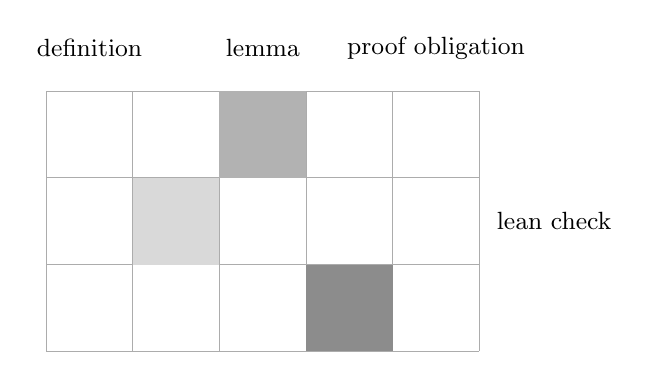
\begin{tikzpicture}[node distance=1.35cm,>=Latex,every node/.style={font=\small}]
\draw[step=1.1cm,gray!65,thin] (0,0) grid (5.5,3.3);
\node[align=center] at (0.55,3.85) {definition};
\node[align=center] at (2.75,3.85) {lemma};
\node[align=center] at (4.95,3.85) {proof obligation};
\node[align=center] at (6.45,1.65) {lean check};
\fill[black!15] (1.1,1.1) rectangle (2.2,2.2);
\fill[black!30] (2.2,2.2) rectangle (3.3,3.3);
\fill[black!45] (3.3,0) rectangle (4.4,1.1);
\end{tikzpicture}
\caption{Formal Knowledge AI Ontologies: evidence matrix of proof dependency pressure 17-1-12}
\label{fig:figure-formal-knowledge-ai-ontologies-and-the-limits-of-taxonom-one}
\end{figure}
The point of the diagram is not decoration; it marks which relation is being proposed and which stronger conclusion is still unavailable.\par
A local clarification is useful here\par
A local clarification is useful here\footnote{In Formal Knowledge AI Ontologies, this note clarifies the reader clarification role of the term and keeps the caveat close to the sentence that needs it.}.\par
The note keeps the caveat near the term without derailing the main sentence.\par
Consider a patient arriving at a clinic with fever, fatigue, a travel history, and an ambiguous test result. A simple taxonomy may place the case under infection, inflammatory disease, or unknown. Each label is useful, but none by itself captures the changing configuration. Symptoms evolve. Test reliability varies. Social exposure matters. Treatment changes future observations. The physician's uncertainty is not an embarrassment outside the system; it is part of the decision field. The problem is not merely choosing the right box. The problem is describing a moving situation without pretending it is already still.\par
Formal knowledge is knowledge made explicit enough for inspection and rule-governed use. It can be written as definitions, logical relations, equations, schemas, or computable procedures. Its power is clarity. Its danger is premature closure. When formal knowledge freezes a living configuration too early, it may preserve consistency at the cost of contact with the phenomenon.\par
This is where metaontology enters. Metaontology asks how ontologies are made, compared, limited, and revised. It asks not only what exists in a model, but what kind of modeling act has declared it to exist. The question is not remote from practice. A hospital record, a legal form, a machine-learning dataset, and a treaty map all contain decisions about what will count as an entity, a relation, an exception, or a change.\par
OC enters this history as a proposed operational metaontology. It is not a replacement for domain science, and it is not a proof that all domains share the same observables. It is a language for comparing how systems are described when simple lists of things no longer suffice: when boundaries move, when processes transform the object being classified, when contradictions expose missing distinctions, and when a model loses the configuration it was meant to hold.\par
\section{What the Tradition Made Visible In Formal Knowledge AI Ontologies}
The oldest taxonomic impulse is reasonable. To think at all, one must distinguish. A plant is not a stone, a fever is not a debt, a promise is not a molecule. Classification gives memory a handle and gives conversation a stable object. Philosophical ontology refined this impulse by asking which distinctions are fundamental and which are merely convenient. The question never belonged only to metaphysics. Every archive, laboratory notebook, legal code, and database repeats it in operational form. \cite{hopfield_nn,hebb_organization}\par
Classical classification tends to favor kinds. A kind is a grouping under a shared description: animal, mineral, contract, infection, signal. Hierarchical classification adds levels: genus, species, subtype, instance. This structure is powerful because it allows inheritance. If all antibiotics are drugs, and a given item is an antibiotic, then the system may inherit drug-related constraints. In computational settings, that inheritance can be automated.\par
The local dependency can now be written without changing the claim it supports.\par
\begin{equation}\label{eq:equation-formal-knowledge-ai-ontologies-and-the-limits-of-taxonom-two}
\operatorname{physicalContinuity}_{3} = \kappa_{K_3}=\frac{b_{K_3}+s_{K_3}}{1+o_{K_3}+q_{K_3}}
\end{equation}
The relation names a local dependency, variable dictionary, and proof/evidence role; it is not a claim-status upgrade.\par
The formula is a restraint on the prose. It names the dependency that the surrounding paragraph is allowed to use.\par
The comparison below gives formal knowledge ai ontologies a set of quantities that can be inspected instead of merely admired.\par
\begin{table}[htbp]
\centering\small
\caption{Formal Knowledge AI Ontologies: observable quantities and counter-pressure 17-2-12}
\label{tab:table-formal-knowledge-ai-ontologies-and-the-limits-of-taxonom-one}
\begin{tabular}{@{}llll@{}}
\toprule
Question & Observed cue & Local value & Reader use \\
\midrule
formal knowledge ai ontologies boundary & 45 units & declared case & fixes what is compared \\
residual pressure & 0.14 & dimensionless & shows unresolved load \\
projection loss & 0.78 & bounded interval & marks lost structure \\
countercase set & 20 cases & review sample & keeps a falsifier visible \\
\bottomrule
\end{tabular}
\end{table}
The table should be read locally: it narrows the comparison without pretending that the wider theory has been settled by a single surface.\par
Artificial intelligence inherited this ambition. Early knowledge systems needed explicit representations of the world so that machines could answer questions, infer missing relations, and support decisions. A medical ontology could connect symptoms to syndromes. A manufacturing ontology could connect parts to assemblies. A geographic ontology could connect roads, rivers, addresses, and administrative regions. The shared hope was that reliable formal structure would make reasoning portable.\par
The hope was not foolish. Without formal structure, machine reasoning becomes brittle in another way: it cannot tell whether two names refer to the same kind of thing, whether one relation implies another, or whether a rule has been applied outside its intended range. Taxonomy, schema, and ontology are among the ways a system resists chaos. They make knowledge communicable.\par
But communication is not identity with reality. Shannon's mathematical theory of communication deliberately separated the engineering problem of transmitting signals from the semantic problem of meaning. That distinction remains instructive here: a message can be encoded, transmitted, and decoded with great precision while the referent remains uncertain or disputed. Formal ontologies can improve the transmission and manipulation of structured claims without guaranteeing that the world has the same joints as the representation.\par
Learning systems introduced another pressure. Hebb's account of neural organization treated learning as a change in connection patterns rather than as the mere filing of propositions. In simplified terms, repeated co-activity can alter future responsiveness. This matters for ontology because cognition may not begin as a table of named entities. It may begin as patterned sensitivity, strengthened pathways, and emergent distinctions that become nameable only later.\par
Hopfield's neural network model added a second lesson. In such networks, memory can be represented as stable states toward which the system settles. A disturbed pattern may move toward a stored configuration. The model does not say that all thought is a Hopfield network, but it offers a concrete image: knowledge can be dynamic, attractor-like, and state-dependent rather than merely taxonomic.\par
Friston's free energy principle places this pressure in a broader theoretical idiom. Organisms and adaptive systems can be described as acting to reduce uncertainty relative to their models of the world. The claim is mathematically ambitious and debated in scope, but for this chapter its relevance is narrower: intelligent systems are not only containers of labeled objects. They are also systems that update, regulate, and maintain workable relations between internal states and external conditions.\par
\section{Where the Inheritance Runs Out In Formal Knowledge AI Ontologies}
The gain from formal ontology is best seen where confusion would otherwise be immediate. Suppose a hospital, a research database, and a public health agency all record the same outbreak. One system stores patients, another stores viral sequences, another stores locations and exposure events. Without shared terms, the records cannot be compared. With a controlled ontology, the systems can distinguish a person from a specimen, a specimen from a test, a test from a result, and a result from an interpretation. \cite{hopfield_nn,hebb_organization}\par
This is not cosmetic order. If the ontology says that every test result must be linked to a specimen, and every specimen must be linked to a collection time, then missing data can be found. If a diagnosis is defined as a clinical judgment rather than a laboratory event, then a positive assay does not automatically become a disease claim. The ontology protects distinctions that matter.\par
The local dependency can now be written without changing the claim it supports.\par
\begin{equation}\label{eq:equation-formal-knowledge-ai-ontologies-and-the-limits-of-taxonom-one}
\operatorname{chemicalPathway}_{3} = \operatorname{support}(c_{3})=P(c_{3})\wedge E(c_{3})\wedge R(c_{3})
\end{equation}
The relation names a local dependency, variable dictionary, and proof/evidence role; it is not a claim-status upgrade.\par
The formula is a restraint on the prose. It names the dependency that the surrounding paragraph is allowed to use.\par
The local dependency can now be written without changing the claim it supports.\par
\begin{equation}\label{eq:equation-formal-knowledge-ai-ontologies-and-the-limits-of-taxonom-three}
\operatorname{cognitiveLoad}_{3} = \operatorname{falsify}(h)=\exists e\in E\,:\,\operatorname{pred}_h(e)\neq\operatorname{obs}(e)
\end{equation}
The relation names a local dependency, variable dictionary, and proof/evidence role; it is not a claim-status upgrade.\par
The formula is a restraint on the prose. It names the dependency that the surrounding paragraph is allowed to use.\par
A small numerical test keeps the abstraction honest at the scale of a single decision.\par
\paragraph{Numerical example.} For formal knowledge ai ontologies, take support=0.51, projection loss=0.13, and 6 open obligations. The bounded score is 0.; the example gives the reader a numeric scale without pretending to be empirical proof.\par
The numbers are deliberately small; their value is pedagogical, not evidential, unless the chapter binds them to a dataset elsewhere.\par
A taxonomy also permits compression. A clinician does not need to list every known property of a drug each time it appears in a record. The drug can inherit class-level information: route, interaction families, contraindication categories, or regulatory status. The system becomes usable because repeated structure is not rewritten from scratch.\par
Formal knowledge makes disagreement sharper. If one researcher says that a case belongs under autoimmune disease and another says it belongs under infection, the ontology can reveal whether they disagree about symptoms, causal mechanism, temporal sequence, diagnostic threshold, or naming convention. A dispute that began as a clash of labels can become a dispute over a specific relation.\par
This is the strongest case for AI ontologies. They do not merely sort words. They can expose hidden assumptions, support audit, preserve distinctions across institutions, and allow rule-governed inference. When used with care, they reduce ambiguity without requiring omniscience.\par
The gain extends beyond medicine. In ecology, an ontology can distinguish habitat, population, species, observation, instrument, and sampling method. In law, it can distinguish person, office, authority, obligation, violation, and remedy. In engineering, it can distinguish component, function, failure mode, interface, and operating condition. Each domain has its own observables, but each benefits from explicit structure.\par
Urban life gives a humbler example. A transit agency may classify stops, routes, vehicles, zones, schedules, fares, delays, and accessibility conditions. Riders experience these categories as practical affordances rather than as metaphysical claims. The map, the ticketing system, and the timetable work because they omit most of the city and preserve a narrow structure of movement. The formal model is useful because it is partial in a disciplined way.\par
The point is not that ontology should become modest in the sense of weak. It should become precise about its strength. A formal representation is not stronger because it is written in a strict syntax. It is stronger only when the syntax preserves relevant differences, forbids misleading substitutions, and remains revisable when the modeled system changes. A beautifully ordered vocabulary can still be wrong.\par
\section{The Conceptual Debt In Formal Knowledge AI Ontologies}
The limit appears when taxonomy is asked to do work that belongs to process. A tree of categories can represent parent and child classes, but many systems are not primarily trees. They are flows, tensions, feedback loops, thresholds, and transformations. A fever is not only an instance of a symptom class. It is a bodily process with causes, timing, regulation, measurement error, and clinical consequence. \cite{hopfield_nn,hebb_organization}\par
A city district may be classified as residential, commercial, industrial, mixed, or informal. The district may still be changing faster than the category system. A street can become a market in the morning, a transport corridor in the afternoon, and a social gathering place at night. The category is not useless. It is incomplete when treated as the whole reality.\par
A small numerical test keeps the abstraction honest at the scale of a single decision.\par
\paragraph{Numerical example.} For formal knowledge ai ontologies, take support=0.54, projection loss=0., and 1 open obligations. The bounded score is 0.240; the example gives the reader a numeric scale without pretending to be empirical proof.\par
The numbers are deliberately small; their value is pedagogical, not evidential, unless the chapter binds them to a dataset elsewhere.\par
The case that follows turns the proposal into a sequence of criticizable moves.\par
\paragraph{Worked case.} In the worked case for formal knowledge ai ontologies, the claim is reduced to a boundary, an observable, a dependency, a numerical cue, and a falsifier. The case is useful only because each move can be criticized separately.\par
The case helps because each step can fail separately, which is exactly what a useful example should permit.\par
Taxonomy also struggles with boundary change. A boundary is a distinction that separates one system, region, role, or state from another. Some boundaries are physical, like a membrane. Some are institutional, like a legal jurisdiction. Some are operational, like the difference between a controlled experiment and an uncontrolled field condition. Boundaries can sharpen, blur, migrate, or fail.\par
A formal ontology can name boundaries, but naming a boundary is not the same as describing its behavior. A border checkpoint may be open, closed, selectively enforced, bypassed, overloaded, or symbolically present but operationally absent. A disease category may be stable in a textbook but unstable at the bedside. A software interface may be documented yet violated in practice by downstream use.\par
Contradiction introduces a deeper limit. In ordinary logic, contradiction is often treated as a sign that something has gone wrong: two incompatible claims cannot both hold under the same interpretation. That remains essential for formal discipline. But in living systems, scientific modeling, and institutional change, contradictions often appear before a new description is available. The contradiction may signal that an old vocabulary no longer spans the phenomenon.\par
For example, a biological entity may behave like a discrete organism in one context and like a distributed microbial community in another. A platform company may look like a marketplace to regulators, an employer to workers, a software provider to developers, and an infrastructure dependency to businesses. The contradiction is not solved by choosing one label too quickly. It may require a richer account of level, boundary, and relation.\par
This does not license vague thinking. The answer to taxonomic failure is not to abandon distinctions. The answer is to ask which distinctions are being made, at what level, through which operation, and with what known loss. Measurement changes what can be seen. Classification changes what can be grouped. Aggregation changes what can be counted. Filtering changes what can be ignored. Intervention changes what will happen next. These acts are not passive windows. They are operators: actions, rules, transformations, or procedures that change a configuration or make a relation visible.\par
Projection is especially important. A projection is a disciplined reduction of a richer system into a narrower view. A subway map projects a city into stations and lines. It omits elevation, building ownership, air quality, and street life. The omission is not an error if the map is used for transit navigation. It becomes an error if the map is mistaken for the city.\par
AI ontologies often fail at the point where projection is forgotten. A class hierarchy is a projection. A database schema is a projection. A training label is a projection. A benchmark task is a projection. Once this is admitted, the central question changes: not whether the model contains the world, but whether it declares the conditions and losses of its own projection.\par
A compact example is schema drift in a model trained to classify customer requests. During training, the category refund may mean a completed purchase reversed after payment. Six months later, the business introduces subscriptions, partial credits, loyalty points, chargebacks, and automated renewals. Customers still write the word refund, but the operational meaning has split across billing states, contractual terms, and user expectations. A classifier may continue to score the old label confidently while routing cases badly. The problem is not only that the model has aged. The label itself has become a projection of a business process that has changed beneath it.\par
Benchmark categories can create a similar illusion. A system may perform well on a task called question answering while the benchmark rewards pattern completion, document lookup, or answer style rather than robust understanding. The category names a competence, but the measurement may capture a narrower operation. When the benchmark is treated as the thing itself, formal success can conceal conceptual drift.\par
\section{The Passage to Continua In Formal Knowledge AI Ontologies}
A successor layer to taxonomy becomes necessary when three pressures coincide: the system changes over time, the boundaries are not fixed, and contradiction carries information rather than mere noise. In such cases, a list of kinds remains useful but insufficient. The model must be able to speak about continua, transitions, operators, projections, and the loss of configurations that can no longer hold. \cite{hopfield_nn,hebb_organization}\par
A continuum is a field of possible variation rather than a single box. Temperature is a simple example. Health, attention, social legitimacy, ecological resilience, and institutional control are more difficult examples. They may not be measurable on one universal scale, but they often vary by degree, threshold, and relation. A continuum does not erase categories. It explains why categories sometimes appear, shift, and fail.\par
Return to the clinic. A patient's symptoms do not fit the available disease categories. One response is forced classification: choose the least bad label and move on. Another response is indefinite uncertainty: refuse to classify at all. A third response asks whether the contradiction reveals a missing dimension: time course, exposure network, immune state, measurement regime, or interaction between conditions. If the missing dimension can be specified, the case becomes describable in a new way. If it cannot, the diagnostic configuration may remain unstable.\par
At this point the word collapse can be used with more care. Collapse names the loss of a configuration that can no longer maintain itself under its tensions, conditions, or operations. In a bridge, collapse may be physical. In an argument, it may be logical. In an institution, it may be procedural or normative. In a model, it may occur when the model cannot absorb observed variation without contradiction or arbitrary repair.\par
The central OC hypothesis belongs here: an unresolved contradiction either gives rise to a new dimension of description or collapses the configuration that cannot resolve it. In this chapter, that sentence has the status of a proposed organizing hypothesis, not a settled theorem and not an empirical conclusion. Its value at this stage is explanatory orientation. It tells the reader what kind of phenomena the later formal vocabulary is being built to describe.\par
The movement appears in AI knowledge systems with particular force. An ontology built for static objects may fail when asked to represent adaptive agents. A taxonomy built for products may fail when products become services, platforms, subscriptions, and data pipelines at once. A legal classification may fail when a technical system occupies several institutional roles simultaneously. These failures are not always defects of implementation. Sometimes they show that the ontology's underlying dimensions are too few.\par
Successor pressure therefore does not mean that taxonomy is obsolete. It means taxonomy must be placed inside a larger account of modeling. Categories become local instruments. Relations become conditional. Boundaries become objects of analysis. Operators become explicit. Continua explain variation. Collapse marks the failure of a configuration. Contradiction becomes a diagnostic event whose handling must be disciplined.\par
The objection is predictable: if everything becomes continua, operators, and projections, does the model lose the crispness that made formal knowledge useful? The answer is no, provided the vocabulary does not dissolve distinctions into atmosphere. A continuum must be named with the relevant dimension of variation. An operator must specify what it transforms or reveals. A boundary must be described by its function and failure modes. A projection must declare what it preserves and what it discards.\par
A second objection is that such a vocabulary may become too general to test. That danger is real. A metaontology that can explain every outcome after the fact explains too much. OC avoids that danger only if later claims are stated with bounded domains, explicit definitions, and rejection conditions. This chapter does not establish that the later apparatus succeeds. It prepares the conceptual need for such apparatus and names the discipline it must satisfy.\par
\section{A Problem Older Than the Vocabulary In Formal Knowledge AI Ontologies knowledg}
OC begins from a simple refusal: a system is not adequately described merely by listing the things inside it. The list matters, but so do the continua along which the system varies, the boundaries that hold or fail, the operators that transform it, and the contradictions that expose missing dimensions. This is why OC is introduced as an operational metaontology rather than as another domain ontology. \cite{hopfield_nn,hebb_organization}\par
Operational means that the vocabulary is intended for use in making descriptions inspectable. A boundary must do descriptive work. A continuum must organize variation. An operator must change, reveal, translate, or constrain something. A projection must be accountable for its losses. These terms are not decorative. They are meant to prevent the model from hiding behind impressive abstraction.\par
The bridge from AI ontology to OC is therefore not rejection but incorporation. Classifications remain necessary. Controlled vocabularies remain necessary. Formal schemas remain necessary. What changes is their rank. They are no longer treated as the deepest form of order. They become one family of projections within a broader account of systems under transformation.\par
This broader account is needed before later scientific claims can be read fairly. If a later section speaks about a boundary, the reader must know that a boundary is not only a line on a diagram. If it speaks about a continuum, the reader must know that a continuum is not a vague synonym for complexity. If it speaks about contradiction, the reader must know that contradiction is not being romanticized as insight. It is being treated as a condition that either forces a new descriptive dimension or marks failure.\par
The AI lineage clarifies the stakes. Shannon helps separate signal handling from meaning. Hebb helps show that learning may begin as changed organization rather than explicit symbolic inventory. Hopfield helps picture knowledge as dynamic stabilization. Friston helps frame adaptive systems as maintaining workable relations under uncertainty. None of these sources proves OC. Together, they make it harder to believe that a flat taxonomy is enough for systems that learn, regulate, transform, and fail.\par
The final point is scientific restraint. OC can propose a language for cross-domain comparison without claiming that every domain reduces to one substrate, one metric, or one proof style. A legal boundary, a cellular membrane, and a software interface are not the same kind of object. OC may compare them only by carefully stating the level of description, the relevant operators, and the losses introduced by projection.\par
The handoff is now in place. Formal knowledge gives clarity, inheritance, audit, and machine-usable structure. AI ontologies show how powerful that structure can be, and how quickly it strains under time, boundary change, projection, and contradiction. OC begins at that strain. It asks what must be added so that categories remain useful without pretending to be complete. Later scientific claims can then be approached with the right caution: not as a victory over taxonomy, but as an attempt to describe the conditions under which taxonomy works, fails, and must be supplemented by a more operational account of change.\par
\chapter{Why OC Appears at This Point in the Lineage}
\section{A Problem Older Than the Vocabulary In OC Appears at Point}
Every inquiry into systems begins with a deceptively simple question: what is the thing being described? The question sounds elementary until the object changes while it is being observed. A cell divides. A market reprices. A storm gathers a boundary and then loses it. A person changes a conviction after hearing an argument. A scientific field revises the categories by which it names its own evidence. In each case, the object is not merely a lump with properties. It is a continuing arrangement whose identity depends on relations, thresholds, histories, and modes of description. \cite{hebb_organization,friston_free_energy}\par
Ontology is the discipline that asks what kinds of things exist. Metaontology asks a second-order question: what kind of language lets us say what exists without smuggling in the answer beforehand? The Operational Continuum, abbreviated hereafter as OC, enters at this second level. It is a proposed language for describing systems whose continuity, boundaries, conflicts, and transformations matter to the claim being made. It does not begin by announcing a completed theory of reality. It begins by asking how a description can remain disciplined when the system under description is changing, partly observed, and differently bounded by different inquiries.\par
The next diagram slows the argument down just enough to show how oc appears at point is being organized.\par
\begin{figure}[htbp]
\centering
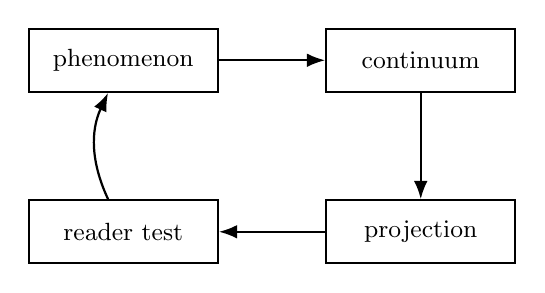
\begin{tikzpicture}[node distance=1.35cm,>=Latex,every node/.style={font=\small}]
\node[draw,thick,align=center,minimum width=2.4cm,minimum height=0.8cm] (a) {phenomenon};
\node[draw,thick,align=center,minimum width=2.4cm,minimum height=0.8cm,right=of a] (b) {continuum};
\node[draw,thick,align=center,minimum width=2.4cm,minimum height=0.8cm,below=of b] (c) {projection};
\node[draw,thick,align=center,minimum width=2.4cm,minimum height=0.8cm,left=of c] (d) {reader test};
\draw[->,thick] (a) -- (b);
\draw[->,thick] (b) -- (c);
\draw[->,thick] (c) -- (d);
\draw[->,thick,bend left=25] (d) to (a);
\end{tikzpicture}
\caption{OC Appears at Point: phase diagram of conceptual dependency pressure 18-1-13}
\label{fig:figure-why-oc-appears-at-this-point-in-the-lineage-one}
\end{figure}
The point of the diagram is not decoration; it marks which relation is being proposed and which stronger conclusion is still unavailable.\par
A local clarification is useful here\par
A local clarification is useful here\footnote{In OC Appears at Point, this note clarifies the reader clarification role of the term and keeps the caveat close to the sentence that needs it.}.\par
The note keeps the caveat near the term without derailing the main sentence.\par
Consider a river. At first it seems easy to identify. It has water, banks, a course, a name, and a location on a map. But a river is not the same water from one hour to the next. Its channel shifts. Its seasonal floodplain may be part of the river for one purpose and outside it for another. A legal boundary, an ecological boundary, a hydrological boundary, and a lived boundary for a nearby town need not coincide. The river is real, but its objecthood is not exhausted by a single perimeter.\par
The river shows the problem before any technical vocabulary is needed. A map may show the channel, but the farmer cares about saturation in the soil. The engineer cares about flow rate and levee pressure. The ecologist cares about wetlands, sediment, fish passage, and seasonal exchange. The town remembers where the water reached during the last flood. None of these descriptions is automatically false because it omits what another description preserves. Each draws the river under a purpose. The difficulty begins when one description is made to stand for the whole river without saying what it has selected and what it has left aside.\par
This problem becomes sharper when the system is less visibly material. A company, an immune response, a language, a nervous system, or a scientific discipline cannot be described well by listing parts alone. The relevant identity often lies in patterned continuity: what remains stable enough to count as the same system while its constituents, states, and boundaries change. The question is not whether such systems are real. The question is how to describe them without pretending that one domain's observable markers are universal.\par
OC uses the word continuum for a describable field of variation that can preserve some identity across change. A continuum is not simply a smooth line. It is a way of saying that a system can vary along named dimensions while remaining intelligible as the system under inquiry. A room's temperature, a negotiation's level of commitment, a neural assembly's excitation, and uncertainty in a signal are not the same kind of quantity. They should not be treated as if they were. Yet each can be described as a field in which differences matter, thresholds appear, and states may become more or less stable.\par
The opening discipline is restraint. OC cannot begin by claiming that every river, mind, institution, and physical system has already been captured by one master formula. A language that cannot lose is not scientific. A language that collapses all domains into one vocabulary is not useful for serious inquiry. OC is introduced here more modestly: as a vocabulary for keeping continuity, boundary, transformation, uncertainty, and conflict visible while preserving the differences among domains.\par
\section{What the Tradition Made Visible In OC Appears at Point}
OC appears after a long sequence of attempts to solve the same family of problems. The lineage is not a march from error to truth. It is a record of gains and limits. Each predecessor made something visible and left something unresolved. The point of naming a lineage is not to inherit authority from it, but to show why a vocabulary like OC becomes plausible only after certain older vocabularies have done their work. \cite{hebb_organization,friston_free_energy}\par
The oldest pressure comes from the problem of being itself. To call something a thing is already to draw a boundary. A stone seems to invite that boundary. A flame complicates it. A city complicates it further. A city has roads, buildings, laws, habits, traffic rhythms, memories, exclusions, and expectations. Its matter changes while its name persists. It is neither pure substance nor pure event. Any ontology that treats it only as an object loses its becoming; any ontology that treats it only as becoming loses the constraints that let it be recognized.\par
The local dependency can now be written without changing the claim it supports.\par
\begin{equation}\label{eq:equation-why-oc-appears-at-this-point-in-the-lineage-two}
\operatorname{technologyCoupling}_{4} = C_{\mathrm{unres}}=\min_{\pi\in\Pi}\|B(x)-B(\pi x)\|
\end{equation}
The relation names a local dependency, variable dictionary, and proof/evidence role; it is not a claim-status upgrade.\par
The formula is a restraint on the prose. It names the dependency that the surrounding paragraph is allowed to use.\par
The comparison below gives oc appears at point a set of quantities that can be inspected instead of merely admired.\par
\begin{table}[htbp]
\centering\small
\caption{OC Appears at Point: observable quantities and counter-pressure 18-2-13}
\label{tab:table-why-oc-appears-at-this-point-in-the-lineage-one}
\begin{tabular}{@{}llll@{}}
\toprule
Boundary & Measured cue & Scale & Failure sign \\
\midrule
oc appears at point boundary & 48 units & declared case & fixes what is compared \\
residual pressure & 0.21 & dimensionless & shows unresolved load \\
projection loss & 0. & bounded interval & marks lost structure \\
countercase set & 21 cases & review sample & keeps a falsifier visible \\
\bottomrule
\end{tabular}
\end{table}
The table should be read locally: it narrows the comparison without pretending that the wider theory has been settled by a single surface.\par
Modern scientific description added the pressure of measurement. A measured system must expose variables. The variable is one of the great achievements of scientific thought because it allows change to be stated without giving up rigor. But variables also introduce choices. What is being varied? Which dimensions are treated as relevant? Which differences are ignored? A description of a forest by biomass, species count, carbon exchange, legal ownership, or sacred significance may refer to the same place while constructing different objects of inquiry.\par
Information theory clarified another part of the problem. In the twentieth century, Claude Shannon's mathematical theory of communication separated the technical problem of transmitting signals from the semantic problem of what those signals mean. That distinction remains indispensable. It lets uncertainty, channel capacity, and noise be treated with precision without pretending that a communication system has thereby solved meaning, action, or truth. OC inherits this discipline by refusing to treat information, meaning, and system identity as interchangeable.\par
Probability theory added a further correction. Edwin Jaynes argued for probability as a disciplined calculus of plausible inference, not merely a narrow frequency count. That view matters here because many system descriptions operate under incomplete information. A scientist may have measurements, prior assumptions, models, and constraints without possessing total access to the system. OC does not convert incompleteness into certainty. It treats uncertainty as part of the description that must be carried openly rather than hidden inside confident nouns.\par
Learning theory and neuroscience supply another strand. Donald Hebb's account of organization in behavior helped make it natural to think of cognition in terms of adaptive structure: repeated relations can alter future responsiveness, and organization can be built through activity rather than imposed from outside. The relevance for OC is not that brains become the template for all systems. The relevance is that a system may acquire structure through its own history, and that description must sometimes include the way prior states condition future states.\par
Contemporary work on adaptive systems gives still another strand. Karl Friston's free energy principle is one influential attempt to analyze self-organizing systems through bounded states, prediction, and the reduction of certain forms of uncertainty. OC does not take that framework as a settled explanation of every system. It treats it as an example of a broader modern tendency: systems are increasingly described through boundaries, internal states, exchanges with an environment, and the maintenance or failure of organization under constraint.\par
Across these strands, the problem shifts. It is no longer simply to say what exists. It is to say how an entity remains describable while undergoing change, how its boundary is drawn for a given inquiry, how uncertainty enters the account, and how conflicts within a description are handled. OC appears where objecthood, process, information, inference, adaptation, and boundary conditions must be coordinated without being confused.\par
\section{Where the Inheritance Runs Out In OC Appears at Point}
Each predecessor gave inquiry a real gain. Object ontology gave durability. It allowed a claim to be about this body, this instrument, this law, this text, this organism. Without objecthood, inquiry dissolves into flux. A measurement must be made of something. A contradiction must be located somewhere. A theory must say what its terms refer to. OC keeps this gain by preserving the need for bounded description. \cite{hebb_organization,friston_free_energy}\par
Process thinking gave motion back to ontology. It made clear that some entities are badly described when treated as static bearers of properties. A storm is not a marble with weather attached. A storm is organized activity. A metabolism is not a box containing reactions; it is a continuing pattern of transformations. A conversation is not a heap of sentences; it is a temporal exchange in which each move changes the space of possible next moves.\par
The local dependency can now be written without changing the claim it supports.\par
\begin{equation}\label{eq:equation-why-oc-appears-at-this-point-in-the-lineage-one}
\operatorname{agencyChoice}_{4} = \Delta d=\operatorname{rank}(A_{\mathrm{new}})-\operatorname{rank}(A_{\mathrm{old}})
\end{equation}
The relation names a local dependency, variable dictionary, and proof/evidence role; it is not a claim-status upgrade.\par
The formula is a restraint on the prose. It names the dependency that the surrounding paragraph is allowed to use.\par
The local dependency can now be written without changing the claim it supports.\par
\begin{equation}\label{eq:equation-why-oc-appears-at-this-point-in-the-lineage-three}
\operatorname{aiAlignmentProxy}_{4} = P_{\mathrm{collapse}}=\sigma(\alpha R-\beta S-\gamma M)
\end{equation}
The relation names a local dependency, variable dictionary, and proof/evidence role; it is not a claim-status upgrade.\par
The formula is a restraint on the prose. It names the dependency that the surrounding paragraph is allowed to use.\par
A small numerical test keeps the abstraction honest at the scale of a single decision.\par
\paragraph{Numerical example.} For oc appears at point, take support=0.57, projection loss=0.11, and 2 open obligations. The bounded score is 0.153; the example gives the reader a numeric scale without pretending to be empirical proof.\par
The numbers are deliberately small; their value is pedagogical, not evidential, unless the chapter binds them to a dataset elsewhere.\par
Information theory gave a way to speak precisely about uncertainty and transmission. In a communication channel, the important question may not be what a message means to a person, but how much uncertainty is reduced by receiving it under specified conditions. That abstraction is powerful because it narrows the claim. It also teaches a negative lesson: precision is purchased by delimitation. A mathematical theory of signal transmission does not automatically become a theory of understanding.\par
Probabilistic inference gave another gain: it made uncertainty tractable without pretending it had disappeared. In many real systems, the observer cannot know every state. Measurements are partial. Models are revisable. Competing hypotheses may remain live. A disciplined account can still proceed if it states what is known, what is inferred, and what would change the inference. OC inherits this as a rule of intellectual conduct: a proposed description must carry its uncertainty in view.\par
Learning and adaptive-system models gave structure a history. A system may not merely occupy a state; it may become more likely to enter some states because of earlier activity. Neural organization, institutional routine, immune memory, and cultural habit differ in mechanism, but each warns against a purely instantaneous ontology. A system's current boundary and behavior may be unintelligible unless its prior transformations are part of the account.\par
Boundary models gave perhaps the most direct gain for OC. A boundary is not always a wall. It may be a membrane, a convention, a threshold, a statistical distinction, a measurement frame, or a functional closure. The boundary of a cell, a conversation, a market, and a research field are not made of the same stuff. Yet in each case, what crosses the boundary and what remains internal are central to the description.\par
Return to the river. Object language names the river. Process language describes its flow and erosion. Information language can describe sensor readings sent from gauges along its course. Probabilistic language can represent flood risk under uncertain rainfall forecasts. Adaptive-system language can describe how ecosystems and settlements respond to repeated seasonal patterns. Boundary language asks whether the floodplain, delta, aquifer, or legal drainage basin is inside the relevant system. The river has not become six different realities. Six descriptive demands have become visible.\par
The constructive reason OC appears here is that the problem has matured beyond a choice between static thing and changing process. The modern object of inquiry often requires layered description. A system may be materially extended, temporally organized, informationally measured, probabilistically inferred, historically conditioned, and boundary-dependent. A vocabulary that can coordinate these layers becomes useful once the gains of the older models are retained rather than discarded.\par
\section{The Conceptual Debt In OC Appears at Point}
A gain becomes a limit when it is asked to do work it was not built to do. Object language becomes limiting when it treats a changing organization as if its identity were exhausted by a fixed perimeter. Process language becomes limiting when it cannot say what persists through the process. Information language becomes limiting when signal, meaning, and action are blended together without distinction. Probabilistic language becomes limiting when uncertainty is mistaken for arbitrariness or when numerical confidence is treated as ontological completion. \cite{hebb_organization,friston_free_energy}\par
The limit is often hidden by successful local use. A hydrologist may have a valid model for water flow. A lawyer may have a valid boundary for jurisdiction. An ecologist may have a valid description of habitat. A town may have a valid memory of where the river becomes dangerous. Conflict appears when these descriptions are forced into one unmarked vocabulary. One side says the river is here; another says it is there. The disagreement may not be about the water alone. It may be about the descriptive frame.\par
A small numerical test keeps the abstraction honest at the scale of a single decision.\par
\paragraph{Numerical example.} For oc appears at point, take support=0.60, projection loss=0.16, and 3 open obligations. The bounded score is 0.110; the example gives the reader a numeric scale without pretending to be empirical proof.\par
The numbers are deliberately small; their value is pedagogical, not evidential, unless the chapter binds them to a dataset elsewhere.\par
The case that follows turns the proposal into a sequence of criticizable moves.\par
\paragraph{Worked case.} In the worked case for oc appears at point, the claim is reduced to a boundary, an observable, a dependency, a numerical cue, and a falsifier. The case is useful only because each move can be criticized separately.\par
The case helps because each step can fail separately, which is exactly what a useful example should permit.\par
OC calls such a frame a projection. A projection is a disciplined way of describing a system for a domain-specific purpose. The word does not mean illusion. A map projection can distort some features while preserving others because it has a task. In the same spirit, an OC projection preserves what a given inquiry needs while admitting that other projections may preserve different features. This term prevents a common error: assuming that a single successful description has exhausted the system.\par
Another limit appears around contradiction. In ordinary use, a contradiction is a conflict between claims. In OC, the term is narrower: a contradiction is a conflict within a description or configuration that cannot be resolved while preserving the current arrangement of terms, boundaries, or states. The contradiction may be logical, operational, structural, or explanatory. It is not automatically a crisis. It is a sign that the present description may be insufficient for the pressure being placed on it.\par
Imagine a hospital triage system during an emergency. One model sorts patients by immediate physiological risk. Another sorts by available specialist capacity. A third sorts by likely benefit from scarce intervention. A fourth must obey legal and ethical constraints. If all patients can be treated quickly, these descriptions may coexist without strain. Under scarcity, they may conflict. The conflict is not solved by saying that one variable is the real system and the others are decorations. The system has entered a state in which the existing descriptive arrangement cannot satisfy all constraints at once.\par
This is where OC introduces an operator. An operator is an action, transformation, or rule that changes the state of a system or the description of that system. Sorting, filtering, amplifying, suppressing, merging, separating, and translating are general examples. Domain-specific operators must be defined more narrowly when used scientifically. The term is useful because systems do not merely have states; they undergo transformations that may preserve, alter, or collapse the configuration being described.\par
The hospital example shows why operator language matters. A triage protocol is not just a label. It acts on the system by changing priority, routing attention, allocating resources, and making some distinctions consequential. A new rule may create a new descriptive dimension, such as expected time to intervention, that was previously implicit. Or it may expose the failure of an earlier arrangement by making a prior category unusable under emergency conditions. The issue is not only what exists, but what operations make distinctions matter.\par
The limit of predecessor models is most visible at the intersection of boundary, projection, contradiction, and operation. A model may describe a system locally while leaving these intersections ungoverned. OC becomes useful for this class of problems because it asks the description to say which boundary is being used, which projection is active, which operator is applied, what contradiction has appeared, and what would count as resolution or collapse in that context.\par
\section{The Passage to Continua In OC Appears at Point}
A successor vocabulary becomes useful when existing vocabularies remain powerful but no longer coordinate the full problem. The pressure is not fashion. It arises when inquiry faces systems that are dynamic, partially observed, historically conditioned, multi-level, and dependent on boundary choice. The old terms still work locally, but the relation among the terms becomes the unsolved part. \cite{hebb_organization,friston_free_energy}\par
This pressure can be stated without grandiosity. A climate model, a neural model, an economic model, and an organizational model do not share the same observables. Their measurements, scales, and valid interventions differ. Yet they all encounter questions of continuity, threshold, boundary, feedback, and failure. A language for comparing such systems cannot pretend that temperature, belief, liquidity, and trust are the same kind of thing. It must allow comparison at the level of description while preserving domain differences at the level of observation.\par
OC introduces an axis as a dimension along which a system can be described as varying. An axis is not automatically a number line, though it may be quantified in some settings. It is a named dimension of variation relevant to a claim. In a physical system, an axis may involve energy, position, or temperature. In an institutional system, it may involve authority, latency, or compliance. In a cognitive system, it may involve attention, confidence, or prediction error. The scientific burden is to define the axis adequately for the domain rather than merely name it.\par
The terms now fit together. A system is the describable arrangement under inquiry. A boundary marks what is treated as inside, outside, or exchanged across that arrangement for a given purpose. A projection is a domain-specific rendering of the system. An axis names a relevant dimension of variation. A continuum is the field of possible variation across one or more axes. An operator transforms a state or description. A contradiction marks an unresolved conflict within the current arrangement.\par
The successor pressure becomes especially clear when a contradiction does not merely produce an error message but forces a new descriptive dimension. A biological category may fail because developmental history matters. A behavioral category may fail because context changes response. A social category may fail because incentives alter the meaning of the measurement. A physical model may fail at a boundary condition previously ignored. In each case, the failure may reveal an axis the earlier description did not include.\par
OC's central hypothesis belongs here and must be stated with care: an unresolved contradiction either gives rise to a new dimension of description or collapses the configuration that cannot resolve it. This is an organizing hypothesis, not a completed theorem being asserted in advance. It focuses later formal and empirical work. The hypothesis says that contradiction is not merely noise in the account. Under some conditions, it is the site where a system must differentiate, reorganize, or fail.\par
The river gives a simple version. For ordinary navigation, the river may be represented by its channel. During a flood, that representation conflicts with the lived and ecological reality of the river's spread. The contradiction can be handled by adding a floodplain dimension to the description. If institutions refuse that dimension, the old configuration may collapse operationally: maps, insurance rules, emergency plans, and habitat models no longer coordinate. The river did not become mysterious. The prior description lost adequacy under changed conditions.\par
The hospital example gives a higher-stakes version. A triage category built for normal flow may fail when scarcity changes the relation between urgency, capacity, and expected benefit. One response is to introduce a new axis, such as resource sensitivity under emergency conditions. Another response is institutional collapse: the old categories remain printed on forms but no longer guide coherent action. The contradiction reveals that the existing model cannot carry the operational load placed on it.\par
An objection arises immediately. Does this language simply redescribe ordinary model revision in more abstract terms? Partly yes, and that is a virtue. OC is not useful if it cannot recover ordinary cases of model revision, boundary adjustment, and category failure. But OC is also interested in the cross-domain pattern by which contradictions force dimensional change or collapse. It asks whether a disciplined vocabulary can describe that pattern without erasing the particular mechanisms in each domain.\par
A second objection is stronger. If every failure can be called a contradiction and every repair can be called a new dimension, the vocabulary becomes unfalsifiable. OC must avoid that. A contradiction must be specified. The prior configuration must be named. The proposed new axis must do work that the earlier description could not do. A collapse claim must identify what coordination failed. Later scientific claims must be judged by whether these elements are explicit enough to be inspected and challenged.\par
This is why OC appears here rather than at the beginning of the lineage. It requires the older achievements. Without objecthood, there is nothing stable enough to track. Without process, change is invisible. Without information theory, uncertainty and transmission are blurred. Without probabilistic discipline, incomplete knowledge becomes either overconfidence or paralysis. Without adaptive models, history and self-organization are underdescribed. OC is a proposed successor vocabulary because those predecessor gains make its problem legible.\par
The word successor does not mean replacement by conquest. A successor vocabulary may preserve its predecessors as local instruments. OC has no reason to replace Shannon's technical theory of communication when the question is channel uncertainty, Jaynes's probability logic when the question is inference under uncertainty, Hebbian organization when the question is activity-shaped learning, or Friston's framework when the question is a specific adaptive-system analysis. The successor role lies in coordination across the places where such vocabularies meet and strain.\par
\section{A Problem Older Than the Vocabulary In OC Appears at Point pressure}
OC therefore functions as a bridge between historical metaontological problems and later scientific claims. The bridge is not a claim that all domains are secretly identical. It is a claim that some descriptive problems recur across domains: how to name a system, how to mark its boundary, how to track variation, how to state transformation, how to register contradiction, and how to distinguish dimensional expansion from collapse. These are not final answers. They are the conditions under which later answers can be made intelligible. \cite{hebb_organization,friston_free_energy}\par
The bridge begins with terminology disciplined enough to prevent premature unity. These terms are deliberately general, but they are not meant to remain vague. Their use becomes scientific only when a domain supplies observables, constraints, and rejection conditions. In a physical setting, an axis may be measurable in established units. In a cognitive setting, it may require experimental operationalization. In a social setting, it may require institutional indicators and careful limits. OC does not license a shortcut from metaphor to evidence. It supplies a grammar in which more specific work can be stated.\par
A concrete example can hold the bridge together. Suppose a coastal city is planning for sea-level rise. The city is a system, but not one with a single obvious boundary. Its legal boundary, drainage basin, commuter region, electrical grid, insurance market, and cultural identity may each define a different projection. Sea level, storm frequency, infrastructure age, tax capacity, evacuation time, and public trust may function as axes in different analyses. The continuum is not one smooth master scale; it is the structured field in which those axes vary and interact.\par
Operators enter when the city acts or is acted upon. A zoning change, seawall construction, insurance withdrawal, migration pattern, sensor deployment, or emergency order transforms the system. Some operators alter material exposure. Others alter incentives or information. Others alter institutional legitimacy. A contradiction appears when the current arrangement cannot satisfy its own constraints: for example, when the city must encourage coastal retreat for safety while preserving a tax base dependent on coastal property values. That contradiction is not solved by naming one side real and the other secondary.\par
The contradiction may force a new dimension of description. The city may need to add fiscal exposure as a formal axis in climate planning, distinguish legal residency from functional daytime population, or model trust as a condition for evacuation compliance. If it refuses the new dimension, collapse may occur in a local and practical sense: plans remain official but cease to coordinate action. Emergency routes fail to match actual movement. Insurance signals diverge from zoning signals. Public communication loses credibility. The configuration does not vanish; it stops working as an organized guide.\par
This example also shows the discipline OC requires. It would be illegitimate to claim that the city case proves the whole theory. It illustrates why the vocabulary is useful. Evidence would require defined data, methods, comparisons, and possible failure conditions. Formalization would require precise structures. A theorem would require stated assumptions and valid derivation. A simulation would require reproducible rules and interpretation limits. OC's opening prose can prepare those later stages, but it cannot silently borrow their authority.\par
The handoff is conceptual rather than triumphant. OC appears at this point in the lineage because inherited models have made a new problem visible: systems must be described across continuity and change, boundedness and exchange, uncertainty and inference, local projection and cross-domain comparison. The proposed vocabulary tries to meet that problem without flattening domains into sameness or dissolving them into unrelated fragments.\par
The chapter therefore closes where the next inquiry begins. OC is not the abandonment of older vocabularies, and it is not a promise that every system will submit to one pattern. It is a disciplined proposal for working where established descriptions meet their limits: where a river exceeds its mapped channel, where a hospital's categories fail under scarcity, where a city cannot act coherently until a hidden axis becomes explicit. At that point, the question is no longer whether another vocabulary can be invented. The question is whether this vocabulary can make its claims precise enough to be tested, limited, corrected, and used.\par
\part{motivation}
\chapter{The General Motivation: What Current Models Cannot Measure Together}
\section{The Practical Pressure In General Motivation Current Models}
Modern systems often fail at their joins. A city does not flood only as hydrology, does not overheat only as meteorology, and does not lose power only as engineering. A hospital does not become overloaded only as medicine, staffing, logistics, finance, or psychology. Each description is real. Each selects part of the situation and leaves other parts outside its frame. The practical difficulty is not that knowledge is absent. The difficulty is that different kinds of knowledge often cannot be measured together without flattening the very situation that made the knowledge necessary. \cite{friston_free_energy,shannon_communication}\par
Imagine a clinic during a power outage. To an engineer, the first question may concern circuits, backup supply, equipment load, and restoration time. To a physician, the same event appears as oxygen support, refrigeration of medicine, patient vulnerability, and triage. To an administrator, it raises staffing, liability, transport, and continuity of records. To a family member, it may be a question of trust: who knows what is happening, who can be reached, and whether an instruction can be followed. None of these descriptions is a metaphor for the others. None is the whole event by itself. The outage is electrical, medical, institutional, informational, and human at once.\par
The next diagram slows the argument down just enough to show how general motivation current models is being organized.\par
\begin{figure}[htbp]
\centering
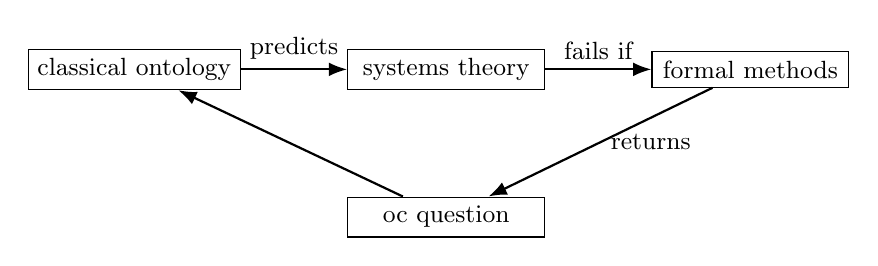
\begin{tikzpicture}[node distance=1.35cm,>=Latex,every node/.style={font=\small}]
\node[draw,align=center,minimum width=2.5cm] (c) {classical ontology};
\node[draw,align=center,minimum width=2.5cm,right=of c] (t) {systems theory};
\node[draw,align=center,minimum width=2.5cm,right=of t] (f) {formal methods};
\node[draw,align=center,minimum width=2.5cm,below=of t] (r) {oc question};
\draw[->,thick] (c) -- node[above]{predicts} (t);
\draw[->,thick] (t) -- node[above]{fails if} (f);
\draw[->,thick] (f) -- node[right]{returns} (r);
\draw[->,thick] (r) -- (c);
\end{tikzpicture}
\caption{General Motivation Current Models: falsifier of historical sequence pressure 19-1-14}
\label{fig:figure-the-general-motivation-what-current-models-cannot-measur-one}
\end{figure}
The point of the diagram is not decoration; it marks which relation is being proposed and which stronger conclusion is still unavailable.\par
A local clarification is useful here\par
A local clarification is useful here\footnote{In General Motivation Current Models, this note clarifies the reader clarification role of the term and keeps the caveat close to the sentence that needs it.}.\par
The note keeps the caveat near the term without derailing the main sentence.\par
Operational Continua, abbreviated here as OC, begins from that kind of case. The name is less important than the discipline it tries to impose. OC treats a system as something described through several directions of variation at the same time. Some directions are easily measured: temperature, voltage, cost, time, pressure, distance. Others are partially measured or only indirectly visible: trust, permission, attention, institutional capacity, public confidence. The purpose is not to pretend that all these things are alike. The purpose is to keep track of their differences when a real decision requires them to meet.\par
The modeling problem is therefore not merely complexity. Complexity names the fact that many parts interact. The harder problem is comparability. One model may measure energy in kilowatt-hours, another may measure risk in probability, another may measure communication in bits, another may measure legal permission as a yes-or-no condition, and another may measure public confidence through surveys, behavior, or proxy signals. These measurements do not naturally share a single ruler. When they are forced into one score too early, the situation becomes easier to rank and harder to understand.\par
A first-time reader needs one discipline before any formal vocabulary appears: the same event can be true under several descriptions, and those descriptions may not be interchangeable. Calling the clinic outage only an electrical event does not make its medical consequences disappear. Calling it all things at once does not automatically explain how the descriptions interact. The gap between these failures is where OC begins.\par
This book will later use terms such as axis, continuum, boundary, operator, projection, contradiction, emergence, and collapse. They should not be heard at first as decorations or as claims of authority. An axis is simply a direction along which something varies. A continuum is the range or field of that variation. A boundary is a distinction that lets one part of a system be treated separately from another without pretending the separation is absolute. These ideas matter because many real situations require more than one axis, more than one continuum, and more than one boundary at the same time.\par
The motivation is not dissatisfaction with the existing sciences. It is dissatisfaction with what happens when their results meet in a real case and no shared operational vocabulary exists for the meeting. Each field may be locally competent. The combined situation may still be unintelligible. OC asks for a restrained way to say what is being measured, what cannot yet be measured, what has been carried from one description into another, and what may be lost in that movement.\par
\section{Why Existing Models Fray In General Motivation Current Models}
A model is a disciplined simplification. It selects variables, defines relations among them, and makes some questions answerable. Selection is not a defect. Without selection there is no model at all. The defect begins when selection is hidden, or when a model built for one purpose is treated as though it had already understood every other purpose that later depends on it. \cite{friston_free_energy,shannon_communication}\par
A climate model can describe heat and rainfall. A grid model can describe supply, demand, equipment stress, and failure propagation. A financial model can describe exposure and cost. A medical model can describe patient risk. A legal model can describe responsibility. None of these models is false because it is partial. The danger comes when the partial model is mistaken for the whole situation, or when outputs from several models are combined before anyone has named what kind of combination is being performed.\par
The local dependency can now be written without changing the claim it supports.\par
\begin{equation}\label{eq:equation-the-general-motivation-what-current-models-cannot-measur-two}
\operatorname{metaTheoryDebt}_{4} = \tau_{\mathrm{repair}}=\inf\{t:C(t)<\theta\}
\end{equation}
The relation names a local dependency, variable dictionary, and proof/evidence role; it is not a claim-status upgrade.\par
The formula is a restraint on the prose. It names the dependency that the surrounding paragraph is allowed to use.\par
The comparison below gives general motivation current models a set of quantities that can be inspected instead of merely admired.\par
\begin{table}[htbp]
\centering\small
\caption{General Motivation Current Models: observable quantities and counter-pressure 19-2-14}
\label{tab:table-the-general-motivation-what-current-models-cannot-measur-one}
\begin{tabular}{@{}llll@{}}
\toprule
Claim & Support carrier & Residual & Interpretation \\
\midrule
general motivation current models boundary & 51 units & declared case & fixes what is compared \\
residual pressure & 0.28 & dimensionless & shows unresolved load \\
projection loss & 0.13 & bounded interval & marks lost structure \\
countercase set & 22 cases & review sample & keeps a falsifier visible \\
\bottomrule
\end{tabular}
\end{table}
The table should be read locally: it narrows the comparison without pretending that the wider theory has been settled by a single surface.\par
If a district is called resilient because expected repair time is low, the statement may have left out residents whose medical devices require power at home. If another model calls the same district vulnerable because many residents are medically dependent, it may have left out the grid design that allows rapid isolation and restoration. Each model may be correct within its frame. Each may mislead when lifted into a wider decision without its frame still visible.\par
OC uses projection for the act of carrying a description from one frame into another. A projection is not automatically wrong. Maps are projections. So are risk scores, dashboards, simulations, executive summaries, and policy categories. The problem is projection loss: the information, distinction, or relation that disappears when a many-sided situation is expressed in a narrower form. A useful projection announces what it has compressed. A dangerous projection forgets that compression occurred.\par
One familiar example is the risk score. A score may combine flood exposure, age of infrastructure, household income, past claims, and emergency access into a single index. The index can help allocate attention. It can also hide the reason a place is at risk. Two neighborhoods may receive the same score for different reasons. One may have high flood exposure and strong emergency access. Another may have moderate flood exposure and weak medical resilience. If both appear as the same number, the model has gained comparability while losing explanation.\par
This is not a complaint against quantification. OC depends on disciplined measurement wherever measurement is available. The objection is to premature unification. A single measure can be legitimate after the relations among its ingredients are understood. It becomes suspect when it arrives before the relevant axes, ranges, and boundaries have been named. A number can summarize a relation. It cannot rescue a relation that was never specified.\par
The point can be seen in the sciences that already handle uncertainty with great seriousness. Claude Shannon's mathematical theory of communication made it possible to study signals, channels, noise, and uncertainty without requiring the engineer to solve the ordinary human problem of meaning. That refusal was a strength. It gave communication theory a clean object. Later treatments, such as the work of Cover and Thomas, show how deep this mathematical tradition becomes when developed through entropy, coding, compression, and inference. Yet a city, hospital, organism, institution, or scientific program may require both the structure of a signal and the practical role that signal plays once it enters a larger arrangement.\par
Probability offers another part of the background. Edwin Jaynes argued for probability as a disciplined logic of plausible inference under uncertainty, not merely a record of frequencies already observed. That matters because many cross-domain decisions are made before exhaustive observation is possible. A hospital does not wait for every outcome to occur before acting during a surge. A power operator does not wait for every failure cascade before shedding load. An institution does not wait for trust to be gone before noticing that its communications are no longer working.\par
Karl Friston's free energy framework supplies a further example of contemporary theory linking uncertainty, prediction, action, and boundary-maintaining behavior. The relevance here is modest. OC does not inherit Friston's mathematics or claim his results as its own. The point is that modern science already contains serious attempts to describe adaptive systems through relations among uncertainty, prediction, action, and boundary. OC belongs to the same broad need for cross-domain language while taking a different task as primary: not to reduce every domain to one formalism, but to make the terms of comparison explicit.\par
\section{The Measurement Gap In General Motivation Current Models}
Current models often struggle when contradiction is treated only as error. In ordinary reasoning, contradiction can mean a mistake: one statement says a thing is so, another says it is not. In lived systems the problem is often more demanding. A contradiction may be a clash among requirements, measurements, or constraints that cannot all be satisfied within the current description. \cite{friston_free_energy,shannon_communication}\par
A hospital may need to reduce crowding and also keep infectious patients separated. A grid may need to cut demand and also preserve power to medically vulnerable residents. An institution may need transparency and also privacy. A school may need to personalize instruction and also protect students from being sorted too early by crude predictions. A factory may need to slow a process for safety while the supply chain requires speed. Some contradictions are resolved by better data. Others reveal that the current description lacks a needed dimension.\par
The local dependency can now be written without changing the claim it supports.\par
\begin{equation}\label{eq:equation-the-general-motivation-what-current-models-cannot-measur-one}
\operatorname{civilizationScale}_{4} = \operatorname{loss}_{\phi}=1-\frac{|E_{\phi}\cap E_{\mathrm{domain}}|}{|E_{\mathrm{domain}}|}
\end{equation}
The relation names a local dependency, variable dictionary, and proof/evidence role; it is not a claim-status upgrade.\par
The formula is a restraint on the prose. It names the dependency that the surrounding paragraph is allowed to use.\par
The local dependency can now be written without changing the claim it supports.\par
\begin{equation}\label{eq:equation-the-general-motivation-what-current-models-cannot-measur-three}
\operatorname{reflexiveLoop}_{4} = I_{\mathrm{axis}}=\frac{\operatorname{Var}(x\mid a)}{\operatorname{Var}(x)}
\end{equation}
The relation names a local dependency, variable dictionary, and proof/evidence role; it is not a claim-status upgrade.\par
The formula is a restraint on the prose. It names the dependency that the surrounding paragraph is allowed to use.\par
A small numerical test keeps the abstraction honest at the scale of a single decision.\par
\paragraph{Numerical example.} For general motivation current models, take support=0.43, projection loss=0., and 4 open obligations. The bounded score is 0.; the example gives the reader a numeric scale without pretending to be empirical proof.\par
The numbers are deliberately small; their value is pedagogical, not evidential, unless the chapter binds them to a dataset elsewhere.\par
This is the point at which OC's central hypothesis enters in its most careful form: an unresolved contradiction either gives rise to a new dimension of description or collapses the configuration that cannot resolve it. This is a proposed way of organizing inquiry, not a completed universal law. It tells the reader what to watch for. When an apparent conflict cannot be handled inside the existing axes, the system may require a new axis, a new boundary, a new operator, or a recognition that the arrangement cannot hold.\par
The claim is easier to see in a small case. Suppose a clinic asks patients to use an online portal for appointments, prescriptions, and test results. The digital model records access: the portal is available, messages are sent, and reminders are delivered. The administrative model sees efficiency. The patient-care model sees missed appointments among older patients, language barriers, disability, and shared phones. The contradiction is not simply that the portal works for some people and fails for others. The deeper problem is that the original model treated access as technical availability, while the lived situation requires a separate axis of practical ability to act. Once that axis is named, the boundary between connected and unconnected patients changes. New operators become visible: phone outreach, translation, proxy authorization, in-person support, paper fallback, or assisted enrollment. If those operators are refused, the clinic may still function technically while its care relation collapses for part of its population.\par
This kind of change is what OC means by a new dimension of description. It is not mystical. It is not a flourish added after the facts. It is the recognition that a system could not be described adequately until a previously hidden direction of variation was made explicit. The contradiction did not merely inconvenience the model. It showed where the model was too flat.\par
An operator, in this vocabulary, is a repeatable transformation that changes a system's state or description. Closing a valve, sending an alert, triaging patients, revising a forecast, imposing a curfew, changing a threshold, adding translation support, or splitting a category can each act as an operator when it transforms the relevant configuration. Operators matter because many failures are not failures of measurement alone. They are failures of action under incompatible descriptions. A model may know that a boundary is stressed, but the available operator may belong to another institution, another time scale, or another vocabulary.\par
The language remains useful only if it stays answerable to cases. It is not enough to say that contradiction is productive, or that new dimensions emerge, or that collapse is possible. One must ask which requirements conflict, which axis is missing, which boundary is doing the wrong work, which operator is unavailable, and what evidence would show that the description has improved. OC is valuable only where such questions become sharper than they were before.\par
\section{The Author's Route Into the Problem In General Motivation Current Models}
Consider a coastal city during a late-summer heat wave followed by heavy rainfall. The city contains dense housing, aging drainage, a strained electrical grid, several hospitals, a port, and neighborhoods with unequal access to transportation. The emergency office receives forecasts of extreme heat, then forecasts of rain, then reports of localized flooding. At the same time, electricity demand rises because air conditioning becomes medically important. The city's problem is not one disaster after another. It is the interaction among several continua that do not share a single scale. \cite{friston_free_energy,shannon_communication}\par
The temperature continuum records heat stress. The water continuum records rainfall, drainage capacity, and flood depth. The electrical continuum records demand, load, equipment stress, and outage risk. The medical continuum records heat illness, respiratory vulnerability, mobility limits, and hospital capacity. The communication continuum records whether warnings reach people in time and whether the instructions can be acted upon. The institutional continuum records who has authority to close roads, open cooling centers, redirect ambulances, or prioritize restoration. Each continuum is partly measurable. None replaces the others.\par
A small numerical test keeps the abstraction honest at the scale of a single decision.\par
\paragraph{Numerical example.} For general motivation current models, take support=0.46, projection loss=0.14, and 5 open obligations. The bounded score is 0.; the example gives the reader a numeric scale without pretending to be empirical proof.\par
The numbers are deliberately small; their value is pedagogical, not evidential, unless the chapter binds them to a dataset elsewhere.\par
The case that follows turns the proposal into a sequence of criticizable moves.\par
\paragraph{Worked case.} In the worked case for general motivation current models, the claim is reduced to a boundary, an observable, a dependency, a numerical cue, and a falsifier. The case is useful only because each move can be criticized separately.\par
The case helps because each step can fail separately, which is exactly what a useful example should permit.\par
At noon, a neighborhood appears stable on the flood map. Its streets are dry. On the heat map, however, it is severe: high surface temperature, many older buildings, and limited tree cover. The public health office wants cooling centers open. The transportation office points out that a main bus route may be interrupted by rain later in the day. The grid operator reports that the circuit serving the area is near its limit. The hospital network reports rising heat-related admissions. No single map is wrong. The difficulty is that the maps are not naturally one map.\par
A common administrative response is to create a priority ranking. Neighborhoods are scored, sorted, and assigned resources. This is often necessary. Scarcity forces order. But the ranking becomes dangerous if it hides why a neighborhood is high priority. A neighborhood with high medical vulnerability and low flood exposure needs different operators from one with high flood exposure and moderate medical vulnerability. The first may need door-to-door checks, cooling transport, backup power, and medical outreach. The second may need pumps, road closures, shelter routing, and drainage clearance. The same score cannot choose the operator unless the underlying axes remain visible.\par
Now add a communication problem. Emergency alerts are sent by phone. The technical system records delivery. In Shannon's terms, transmission can be studied as a problem of signal and channel. Yet delivered is not the same as understood, and understood is not the same as executable. A resident may receive a warning to go to a cooling center but lack transportation. Another may receive a flood warning but be caring for someone who cannot be moved quickly. A third may distrust the instruction because earlier warnings were inaccurate. The communication event crosses from signal transmission into social action.\par
This is where domain projection becomes indispensable and risky. A domain is a field of description with its own variables, methods, and constraints. Hydrology, electrical engineering, medicine, logistics, and public administration are domains in this example. Domain projection occurs when a result from one domain is used inside another. A flood-depth forecast becomes an ambulance-routing constraint. A grid-load forecast becomes a hospital-continuity concern. A hospital-capacity alert becomes a transportation priority. These projections are necessary. They are also places where loss and distortion enter.\par
Suppose a dashboard marks a district red. The color is intended to combine heat risk, flood risk, and outage risk. The mayor asks what to do. The dashboard cannot answer unless its red condition decomposes into actionable relations. Is the district red because the grid is likely to fail, because the hospital serving it is near capacity, because drainage is blocked, because people cannot leave, or because warnings are not being trusted? Each answer implies a different operator. Color is useful for attention. It is insufficient for intervention.\par
OC would describe this case by separating axes, continua, boundaries, operators, and projections before asking for a combined judgment. The neighborhood boundary may be administrative, electrical, hydrological, medical, or social. These boundaries may not coincide. A hospital catchment area can cross a flood zone. A circuit can serve blocks from different districts. A bus route can connect populations that the risk map treats separately. When boundaries do not align, the system cannot be governed well by a single partition.\par
The contradiction now becomes visible. The city may need residents to remain indoors because roads are flooding, while also needing some of them to leave overheated apartments. It may need to reduce electricity demand, while also needing electricity for cooling as a medical intervention. It may need to send simple public instructions, while the real situation requires conditional instructions. These are not merely communication errors. They are structural conflicts among axes. If the city has no vocabulary for the conflicts, it may treat them as failures of compliance, leadership, or data quality when the deeper problem is the missing description of their interaction.\par
What changes when the case is read through OC is not that the city suddenly becomes easy to manage. The change is interpretive discipline. A red district is no longer treated as a single object with a single cause. It becomes a location where several continua intersect, where boundaries may be misaligned, where projections may have hidden losses, and where the correct operator depends on the reason for urgency. The city still needs weather science, grid engineering, medicine, logistics, law, and public communication. OC does not replace them. It gives their meeting a more careful grammar.\par
That grammar can change the questions asked in the room. One analyst can ask whether the flood projection has erased medical immobility. Another can ask whether the grid model treats cooling as discretionary consumption when, for some residents, it is a health requirement. Another can ask whether the communication model treats message delivery as action. Another can ask whether the administrative boundary used for public orders matches the electrical boundary used for restoration. Disagreement becomes more useful because it has locations.\par
The example also resolves the earlier hypothesis in practical form. The contradiction between staying indoors and leaving for cooling may create a new axis: mobility under compound hazard. It may require a new boundary: residents who can safely remain with local cooling support versus residents who must be moved before roads fail. It may require a new operator: pre-positioned cooling transport, mobile power, targeted checks, or building-level cooling support. If none of these descriptions or operators can be created in time, the configuration may collapse: not necessarily as physical destruction, but as the loss of the city's ability to coordinate care, movement, power, and instruction under pressure.\par
\section{What Would Count As Progress In General Motivation Current Models}
The prize is a better way to ask what must be kept distinct before it can be responsibly combined. That may sound restrained, but it is a large practical prize. Many errors in complex systems come from combining too early, separating too late, or treating the wrong boundary as natural. OC seeks an operational metaontology: a language for describing what kinds of things are being compared, how they vary, where their boundaries lie, and what transformations act on them. \cite{friston_free_energy,shannon_communication}\par
Metaontology here means a vocabulary about vocabularies of being, not a claim to replace domain sciences. Ontology asks what kinds of entities and relations a theory admits. Metaontology asks how such ontological choices are organized, compared, and constrained. OC is operational because it is concerned with use: what can be stated, checked, narrowed, rejected, carried across domains, or transformed. The term does not mean that every claim is already implemented in software or proven in a formal system. It means the language is designed around operations rather than decoration.\par
A useful operational language can improve scientific conversation in three ways. First, it can identify the axes in play before they are collapsed into a composite measure. Second, it can mark projection loss when one domain's output becomes another domain's input. Third, it can expose contradictions that require either a new dimension of description or a change in the system's configuration. These are not substitutes for evidence. They are ways of preventing evidence from being misfiled.\par
This also protects pluralism without surrendering rigor. Pluralism means that different domains may require different forms of measurement and explanation. Rigor means that difference cannot be invoked as an excuse for vagueness. An operational metaontology needs both. It must allow medical, electrical, social, informational, legal, and financial descriptions to remain different. It must also require each description to say what it measures, how it transforms, and how it travels into other descriptions.\par
The same structure applies outside crisis. Consider a university trying to evaluate teaching. Student satisfaction, learning outcomes, equity of access, disciplinary difficulty, long-term retention, instructor workload, and intellectual risk are not the same kind of measure. A single score may be administratively convenient, but it can mistake popularity for learning, difficulty for poor teaching, or ease of measurement for importance. The problem is not that evaluation should never be numerical. The problem is that the axes must be named before the number is allowed to stand for them.\par
The role of information theory helps clarify the point. Shannon's theory gained power by refusing to confuse communication engineering with ordinary semantic interpretation. OC takes that lesson seriously. A clean separation of problems can create durable science. But OC also asks what happens after separated problems must meet again in a real system. If transmission, interpretation, trust, mobility, and authority all affect whether a warning changes behavior, then the system needs terms for their meeting without pretending they are the same kind of quantity.\par
The role of probability is similar. Jaynes's account of probability as disciplined uncertainty is valuable because it treats inference as a rational structure rather than a loose feeling. OC can use that spirit while asking a separate question: when uncertain claims from different domains are combined, what has been assumed about their compatibility? The probability of road flooding may be updated hourly from weather and sensor data. The probability that residents will evacuate may depend on trust, past experience, disability, and transport. Both are uncertain. Their uncertainties do not have the same texture.\par
The operational prize is therefore not a universal calculator. It is a disciplined staging area for comparison. Before a model combines, OC asks what is being combined. Before a result travels, it asks what kind of projection is being performed. Before a contradiction is dismissed, it asks whether the contradiction marks a missing axis. Before a boundary is accepted, it asks what work the boundary performs and what it excludes.\par
This is why the book must move slowly at first. Later formal claims will depend on words that cannot remain intuitive slogans. Axis, continuum, boundary, operator, projection, contradiction, emergence, and collapse must each earn a precise role. The present motivation is the place where those words first become necessary. They are introduced because ordinary modeling practice repeatedly encounters situations in which local competence does not guarantee cross-domain intelligibility.\par
\section{The Practical Pressure In General Motivation Current Models motivati}
The risk of failure is not only practical. It is conceptual. A system can fail because a bridge breaks, a hospital fills, a grid trips, or a warning arrives too late. It can also fail because the description guiding action cannot represent the conflict it faces. When description fails, action may still occur, but it becomes poorly aimed. Resources move toward visible numbers while invisible relations decide the outcome. \cite{friston_free_energy,shannon_communication}\par
One failure mode is false unity. False unity appears when different continua are compressed into a single object without preserving the reason for their combination. A composite resilience index may be useful as an entry point, but if it becomes the object itself, the system has lost the distinction between heat resilience, flood resilience, electrical resilience, medical resilience, and institutional resilience. The word resilience then becomes broad enough to travel and vague enough to mislead.\par
A second failure mode is false separation. False separation appears when domains are kept apart even after their interaction becomes the event of interest. The grid team studies load, the health team studies heat illness, the transport team studies road access, and the communications team studies alert reach. Each produces competent reports. The city still fails because no description captures the fact that power for cooling, ambulance access, and public instruction are coupled during the emergency.\par
A third failure mode is boundary inheritance. A boundary made for one purpose is inherited by another purpose without examination. Administrative districts become emergency districts. Billing regions become care regions. Sensor coverage becomes reality coverage. Network diagrams become social diagrams. Once inherited, these boundaries can shape action while escaping scrutiny. OC treats boundaries as operations of description, not as innocent lines.\par
A fourth failure mode is operator mismatch. The system identifies a problem in one domain but applies an operator from another without translating the relation. A social trust problem is treated as a message-frequency problem. A medical vulnerability problem is treated as a general shelter-capacity problem. A grid-stability problem is treated as a public conservation problem even where consumption is medically necessary. Operator mismatch produces activity that looks responsive while missing the controlling relation.\par
A fifth failure mode is contradiction denial. Contradictions are often softened into trade-offs. Some trade-offs are genuine and manageable. Others are signs that the present description cannot carry the situation. If residents must both remain indoors and leave for cooling, the conflict cannot be solved by choosing one instruction for everyone. The system needs new distinctions: who can safely remain, who must move, which routes are viable, which buildings can be cooled locally, which circuits require protection, and which institutions can act in time.\par
Collapse, in this setting, does not have to mean physical destruction. It can mean the loss of a configuration's ability to maintain its organization under the constraints it faces. A queue collapses when triage no longer orders care effectively. A communication system collapses when messages no longer guide action. A governance arrangement collapses when authority exists on paper but cannot transform the situation. These uses require care, and later chapters must distinguish them more precisely.\par
The objection is immediate: does this language merely rename familiar systems thinking? The answer is that familiar systems thinking often recognizes interaction, feedback, and emergence, but recognition alone is not enough. OC's proposed contribution is the discipline of tracking axes, continua, boundaries, operators, projections, contradictions, and collapse in a way that can be narrowed or rejected. It is not enough to say everything is connected. The question is which connections change the description, which change the system, and which disappear when the case is carried into another frame.\par
Another objection is that cross-domain language risks becoming too abstract to help. That risk is real. A meta-level vocabulary can become fog if it floats above cases. OC avoids that only if every term returns to operational use. An axis must say what varies. A continuum must say the range of variation. A boundary must say what distinction is being made. An operator must say what transformation occurs. A projection must say what travels and what may be lost. A contradiction must say which requirements cannot be jointly satisfied under the current description.\par
The need for this kind of language has become harder to avoid because contemporary systems are increasingly coupled while their models remain institutionally separated. Energy, health, climate, finance, logistics, media, computation, and governance now interact at speeds and scales that make isolated competence insufficient. A failure in one domain can become a constraint in another before the first domain has finished explaining itself.\par
Digital infrastructure intensifies the problem. Sensors, dashboards, forecasts, automated alerts, and decision platforms multiply measurements. They also multiply projections. A sensor reading becomes a model input. A model output becomes a ranking. A ranking becomes a budget decision. A budget decision becomes infrastructure. Infrastructure changes the future data. At each step, something is carried forward and something is left behind. The more automated the chain, the more important it becomes to name the losses.\par
Artificial intelligence makes the issue sharper without being the whole issue. Predictive systems can combine large quantities of data across domains, but combination is not comprehension. A model may learn correlations among weather, traffic, admissions, outages, and public messages. It may still lack an explicit account of which boundary it is using, which operator it is recommending, or which contradiction it has discovered rather than solved. The presence of computation does not remove the need for ontology. It makes unexamined ontology more consequential.\par
The present moment also inherits a long scientific tension between reduction and integration. Reduction seeks clarity by isolating parts and mechanisms. Integration seeks realism by reconnecting what isolation separated. Both are necessary. The danger is choosing one as a permanent ideology. OC is motivated by the possibility that some failures arise not because reduction went too far or integration went too far, but because the movement between them was not described with enough care.\par
The greatest risk is overclaiming. A language that helps organize comparison is not the same as evidence that a particular scientific hypothesis is true. A proposed formal vocabulary is not the same as proof that all systems obey it. A useful example is not a dataset. A plausible reconstruction is not a simulation. OC must preserve these distinctions because its own subject matter makes them tempting to blur. The book's scientific discipline begins with refusing to inflate motivation into confirmation.\par
The chapter can therefore close where it began: with systems that fail at their joins. Current models can measure many things well. They can measure heat, water, voltage, cost, risk, signal, probability, and delay with extraordinary power inside the right frame. The problem appears when the frames meet and the relations among them become the event. A theory of continua must show how descriptions remain distinct, how they meet, what is lost when they are projected into one another, and what happens when their meeting produces a contradiction the current system cannot absorb. OC begins as an answer to that demand, modest in its claims but serious in its obligation: to make cross-domain description explicit enough that it can be used, challenged, corrected, and, where necessary, refused.\par
\chapter{Where Separate Domain Models Stop Talking to Each Other}
\section{The Practical Pressure In Where Separate Domain Models}
At eight in the morning, the regional hospital is strained but still recognizable to itself. The emergency department is crowded, though not beyond anything it has seen before. The inpatient wards are nearly full, though a few beds appear available on the screen. The laboratory is running behind, though samples are still moving. The staffing office has gaps, though the minimum numbers can be covered if nobody else calls in sick. The discharge team expects several patients to leave by afternoon. Each part of the institution can describe its own condition in sentences that are true. \cite{shannon_communication,jaynes_probability}\par
By noon, those true sentences no longer add up to a working picture. Ambulances continue to arrive. Several patients need admission, but the wards cannot accept them quickly. Some beds are physically empty but not usable because cleaning is delayed, isolation requirements do not match the waiting patients, or the right staff are not available. Laboratory results are late, so discharge decisions slow down. Nurses who were already stretched spend more time coordinating exceptions. Families grow anxious because explanations arrive in fragments. The emergency department begins holding admitted patients in spaces designed for short stays.\par
The next diagram slows the argument down just enough to show how where separate domain models is being organized.\par
\begin{figure}[htbp]
\centering
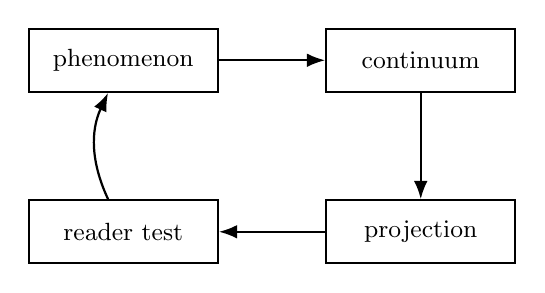
\begin{tikzpicture}[node distance=1.35cm,>=Latex,every node/.style={font=\small}]
\node[draw,thick,align=center,minimum width=2.4cm,minimum height=0.8cm] (a) {phenomenon};
\node[draw,thick,align=center,minimum width=2.4cm,minimum height=0.8cm,right=of a] (b) {continuum};
\node[draw,thick,align=center,minimum width=2.4cm,minimum height=0.8cm,below=of b] (c) {projection};
\node[draw,thick,align=center,minimum width=2.4cm,minimum height=0.8cm,left=of c] (d) {reader test};
\draw[->,thick] (a) -- (b);
\draw[->,thick] (b) -- (c);
\draw[->,thick] (c) -- (d);
\draw[->,thick,bend left=25] (d) to (a);
\end{tikzpicture}
\caption{Where Separate Domain Models: state transition of domain projection pressure 20-1-15}
\label{fig:figure-where-separate-domain-models-stop-talking-to-each-other-one}
\end{figure}
The point of the diagram is not decoration; it marks which relation is being proposed and which stronger conclusion is still unavailable.\par
A local clarification is useful here\par
A local clarification is useful here\footnote{In Where Separate Domain Models, this note clarifies the reader clarification role of the term and keeps the caveat close to the sentence that needs it.}.\par
The note keeps the caveat near the term without derailing the main sentence.\par
No single department has simply lost contact with reality. The clinical team still classifies patients by risk. The bed office still tracks rooms. The staffing office still counts coverage. The laboratory still reports queues. The finance office still records activity. The families still register waiting, fear, and trust. The problem is not that one model is false. The problem is that the models are locally adequate while the hospital is failing between them.\par
This is the kind of situation in which a domain model reaches its limit. A domain model is a disciplined way of describing a class of situations. It decides what counts as an object, what counts as a state, what counts as a change, and what counts as an explanation. In medicine, oxygen saturation, infection markers, renal function, and clinical risk are meaningful. In operations, bed occupancy, cleaning delay, transfer requests, and discharge timing are meaningful. In labor management, staffing ratios, skill mix, fatigue, and absence matter. In finance, reimbursement codes, denial risk, and cost exposure matter. Each model becomes useful by excluding almost everything else.\par
That exclusion is not a mistake. A model that tried to include every relevant fact at once would become unusable. A physician cannot make every clinical decision by consulting the entire financial, logistical, social, and regional context. A bed manager cannot treat every room assignment as a full theory of medicine. A laboratory cannot process specimens by constantly modeling family trust and ambulance flow. Disciplined blindness is part of competence.\par
The trouble begins when the blindness stops being harmless. The hospital under respiratory pressure is not only a medical system, not only an operational system, not only a labor system, and not only a social institution. It is all of these at once, but not as a blur. The domains remain distinct. What changes is that events in one domain start altering the meaning and effectiveness of events in another. A delayed lab result becomes a blocked discharge. A blocked discharge becomes an unavailable bed. An unavailable bed becomes emergency congestion. Emergency congestion becomes nursing overload. Nursing overload becomes slower coordination. Slower coordination becomes more uncertainty.\par
The chapter's title names this failure: separate domain models stop talking to each other. They do not stop producing data. They do not stop serving skilled professionals. They do not even stop being partly right. They stop being sufficient for the shared situation that their own actions are helping to create.\par
\section{Why Existing Models Fray In Where Separate Domain Models}
Modern institutions often fail with excellent records in hand. Their dashboards are populated. Their procedures are written. Their responsibilities are assigned. Their communications are timestamped. Afterward, each unit can often show that it acted according to its own standards. The emergency department can point to triage rules. The wards can point to capacity constraints. The laboratory can point to machine throughput. The staffing office can point to available personnel. Finance can point to contractual realities. The failure survives because everyone can defend a local rationality. \cite{shannon_communication,jaynes_probability}\par
This kind of failure is difficult because it does not look like ignorance from inside the participating domains. It looks like pressure, delay, exception handling, and unfortunate timing. The clinical model says the patient is stable enough to wait. The operational model says no appropriate bed is currently available. The staffing model says adding another patient to the ward would violate safe ratios. The laboratory model says the queue is being processed in order of priority. The family's model says waiting without explanation is becoming abandonment. Each statement can be defensible, and together they can describe a system crossing into danger.\par
The local dependency can now be written without changing the claim it supports.\par
\begin{equation}\label{eq:equation-where-separate-domain-models-stop-talking-to-each-other-two}
\operatorname{historicalInheritance}_{4} = \rho_{\mathrm{replay}}=\frac{N_{\mathrm{matched}}}{N_{\mathrm{declared}}}
\end{equation}
The relation names a local dependency, variable dictionary, and proof/evidence role; it is not a claim-status upgrade.\par
The formula is a restraint on the prose. It names the dependency that the surrounding paragraph is allowed to use.\par
The comparison below gives where separate domain models a set of quantities that can be inspected instead of merely admired.\par
\begin{table}[htbp]
\centering\small
\caption{Where Separate Domain Models: observable quantities and counter-pressure 20-2-15}
\label{tab:table-where-separate-domain-models-stop-talking-to-each-other-one}
\begin{tabular}{@{}llll@{}}
\toprule
Model & Retained insight & Rejected assumption & OC extension \\
\midrule
where separate domain models boundary & 54 units & declared case & fixes what is compared \\
residual pressure & 0.35 & dimensionless & shows unresolved load \\
projection loss & 0.24 & bounded interval & marks lost structure \\
countercase set & 23 cases & review sample & keeps a falsifier visible \\
\bottomrule
\end{tabular}
\end{table}
The table should be read locally: it narrows the comparison without pretending that the wider theory has been settled by a single surface.\par
To speak about such situations, a few terms are needed, but they should be earned by the scene. A continuum is a range along which a system can vary while still being treated as one subject of description. Hospital load can rise or fall. Clinical uncertainty can narrow or widen. Staffing capacity can loosen or tighten. Trust can hold, weaken, or break. These are not the same kind of thing, and they do not share one measurement scale. They are ranges that matter because movement along one can change movement along another.\par
A boundary is a rule of separation that shapes what can pass, what must stop, and what changes meaning when it crosses. A hospital bed is bounded by more than mattress and frame. It is bounded by cleaning status, infection category, staffing availability, documentation, clinical appropriateness, and discharge timing. A ward boundary is not merely a floor plan; it is a rule about which patients can be absorbed safely. A professional role boundary determines who may decide, who may override, and who bears responsibility when normal coordination fails.\par
An operator is a repeatable action, rule, mechanism, or pressure that changes a state in a describable way. A discharge order is an operator when it changes bed availability. A lab result is an operator when it permits a decision. A staffing call is an operator when it changes feasible workload. An ambulance diversion policy is an operator when it moves pressure elsewhere. A family communication protocol is an operator when it changes trust, conflict, or patience. The word does not make these actions identical. It says that each performs a comparable grammatical role: something acts on a configuration and changes what can happen next.\par
A projection is a domain-limited view of the same system. The clinical projection sees oxygen demand, diagnosis, deterioration risk, and treatment urgency. The operational projection sees beds, queues, turnover, and transfers. The labor projection sees coverage, fatigue, skill, and bargaining limits. The social projection sees explanation, legitimacy, confidence, and anger. No projection owns the whole hospital. Each makes some truths visible and others obscure.\par
A contradiction, in this setting, is not merely a disagreement or a pair of inconsistent statements. It is a condition in which requirements, tendencies, or constraints cannot continue together under the current organization. The hospital must preserve clinical safety, maintain flow, respect staffing limits, and sustain public trust. Under ordinary strain, these requirements can coexist. Under coupled strain, the available operators may no longer satisfy them all. The contradiction was not invented by language. Language helps reveal why separate correct descriptions have become jointly inadequate.\par
\section{The Measurement Gap In Where Separate Domain Models}
Return to the hospital at noon. The emergency physician sees a patient who should be admitted for observation. The bed screen shows a potential room, but the room is not truly available. It needs cleaning, the ward is short one experienced nurse, and the patient may require isolation depending on a pending test. The laboratory has the sample, but the machine queue is long because the respiratory season has increased volume across the whole region. The discharge planner is waiting on results for another patient who might free a different bed. The family of the waiting patient asks why admission has not happened when a room appears empty. \cite{shannon_communication,jaynes_probability}\par
If one asks for the cause, the answer depends on where one stands. The emergency department says admissions are blocked. The ward says safe acceptance is not possible. The laboratory says demand exceeds processing capacity. The discharge team says decisions require missing information. The staffing office says the system is operating at the edge of its labor envelope. The family says nobody is explaining the delay. None of these answers is foolish. None is complete.\par
The local dependency can now be written without changing the claim it supports.\par
\begin{equation}\label{eq:equation-where-separate-domain-models-stop-talking-to-each-other-one}
\operatorname{grandSynthesis}_{4} = G=(V_{\mathrm{claim}}\cup V_{\mathrm{evidence}},E_{\mathrm{support}}\cup E_{\mathrm{challenge}})
\end{equation}
The relation names a local dependency, variable dictionary, and proof/evidence role; it is not a claim-status upgrade.\par
The formula is a restraint on the prose. It names the dependency that the surrounding paragraph is allowed to use.\par
The local dependency can now be written without changing the claim it supports.\par
\begin{equation}\label{eq:equation-where-separate-domain-models-stop-talking-to-each-other-three}
\operatorname{methodFalsifier}_{4} = \epsilon_{\mathrm{domain}}=\max_i |y_i-\hat y_i|
\end{equation}
The relation names a local dependency, variable dictionary, and proof/evidence role; it is not a claim-status upgrade.\par
The formula is a restraint on the prose. It names the dependency that the surrounding paragraph is allowed to use.\par
A small numerical test keeps the abstraction honest at the scale of a single decision.\par
\paragraph{Numerical example.} For where separate domain models, take support=0.49, projection loss=0., and 6 open obligations. The bounded score is 0.; the example gives the reader a numeric scale without pretending to be empirical proof.\par
The numbers are deliberately small; their value is pedagogical, not evidential, unless the chapter binds them to a dataset elsewhere.\par
The relevant fact is the coupling. Clinical uncertainty slows discharge. Discharge delay blocks beds. Blocked beds congest emergency care. Congestion increases work per patient. Increased work slows coordination. Slower coordination increases uncertainty and frustration. Anxiety among families forces clinicians and nurses to spend time on explanation and conflict management, which may be necessary and humane, but also changes the labor picture. The same minutes are being claimed by several domains at once.\par
At this point, an apparently simple object changes character. The bed is not a bed in the ordinary sense. It is a junction where clinical status, cleaning, staffing, infection control, documentation, and timing meet. The dashboard may count it as empty, but the system cannot use it until several boundaries open at once. The clinical boundary asks whether the patient fits the ward. The labor boundary asks whether the ward can safely absorb the patient. The infection boundary asks whether the room is appropriate. The documentation boundary asks whether the transfer is authorized. The social boundary asks whether delay remains tolerable to the people living through it.\par
This does not mean every hospital problem requires a new vocabulary. Many problems are local. A machine breaks. A nurse calls in sick. A physician misses a result. A billing rule creates a delay. Ordinary domain expertise can often identify and correct such failures. Cross-domain language becomes necessary when the event of interest is not located inside one domain, but in the way several domains constrain one another.\par
One possible response is reconfiguration. The hospital may create a command structure that links discharge planning, laboratory priority, staffing escalation, bed cleaning, ambulance coordination, and family communication into one operating picture. This new structure does not abolish the clinical, operational, labor, and social projections. It gives them a shared place to meet. It adds a descriptive dimension that had been weak or implicit: coordination capacity.\par
Coordination capacity is not merely the number of meetings or messages. It is the ability of the institution to translate among domains fast enough for action. Can the lab understand which delayed result matters for bed flow? Can bed management understand which empty room is unusable for clinical reasons? Can staffing understand when an additional body is not enough because the missing skill is specific? Can clinicians understand when a medically reasonable delay is socially destabilizing because the family has lost trust? Can administrators see when the system is not just busy, but configured for failure?\par
The alternative to reconfiguration is not always total collapse. A system may degrade slowly. It may create informal workarounds. It may push strain into staff exhaustion, delayed care, regional transfers, or public complaint. It may continue in a damaged state long enough that nobody agrees on when the failure began. Some contradictions persist unnoticed because slack hides them. Some are absorbed by people who pay the cost personally. Some are displaced into another institution or another day. The strongest claim one can responsibly make at this stage is not that contradiction always yields emergence or collapse. It is that unresolved cross-domain contradiction often pressures systems toward new description, local workaround, delayed degradation, or breakdown.\par
That caution matters. The hospital story illustrates a pattern; it does not prove a law. It shows why a new level of description can become necessary before behavior is governable. It also shows why any proposed account must remain vulnerable to correction. Perhaps the decisive cause was a single software outage. Perhaps the laboratory queue mattered less than ambulance policy. Perhaps family trust did not affect operations in this case. Perhaps the coupling was reconstructed afterward by observers who wanted a tidy explanation. A vocabulary that cannot be wrong cannot help.\par
\section{The Author's Route Into the Problem In Where Separate Domain Models}
The difficulty is not solved by saying that the hospital needs better information. Sometimes it does. Bad data can kill. But cross-domain failure can occur even when information is accurate in the narrow sense. Bed counts may be correct. Lab timestamps may be correct. Staffing rosters may be correct. Discharge orders may be correct. The communication channels may function, and still the institution may fail to understand its own condition. \cite{shannon_communication,jaynes_probability}\par
Claude Shannon's mathematical theory of communication drew a powerful distinction between transmitting signals and interpreting meanings. That distinction made it possible to study channel capacity, noise, coding, and information with extraordinary clarity. The lesson for cross-domain systems is not that meaning can be ignored. It is that one must know which problem is being solved. A hospital may transmit a bed status perfectly while failing to convey what that bed status means under staffing shortage, infection rules, and delayed discharge.\par
A small numerical test keeps the abstraction honest at the scale of a single decision.\par
\paragraph{Numerical example.} For where separate domain models, take support=0.52, projection loss=0.12, and 1 open obligations. The bounded score is 0.200; the example gives the reader a numeric scale without pretending to be empirical proof.\par
The numbers are deliberately small; their value is pedagogical, not evidential, unless the chapter binds them to a dataset elsewhere.\par
The case that follows turns the proposal into a sequence of criticizable moves.\par
\paragraph{Worked case.} In the worked case for where separate domain models, the claim is reduced to a boundary, an observable, a dependency, a numerical cue, and a falsifier. The case is useful only because each move can be criticized separately.\par
The case helps because each step can fail separately, which is exactly what a useful example should permit.\par
Probability adds another layer. E. T. Jaynes treated probability as a disciplined extension of logic under uncertainty, not merely a tally of frequencies. That attitude is useful because institutions rarely act with complete knowledge. Yet uncertainty is not removed by assigning numbers to isolated variables. Before probabilities can guide action across domains, one must ask what the variables are about, which boundaries make them comparable, and whether their apparent coupling is causal, conditional, or merely coincidental.\par
Information theory, as developed in rigorous mathematical form by writers such as Thomas Cover and Joy Thomas, warns against loose metaphor. Entropy in a coding problem, uncertainty in a classifier, and disorder in an institution are not the same just because the same word tempts us. Measures can be precise inside one formal setting and misleading when carried into another without translation. Cross-domain thought needs the discipline of information theory more than its borrowed glamour.\par
Social thresholds create a further difficulty. Mark Granovetter's threshold model of collective behavior showed how individual rules can generate collective cascades. A person may act only when enough others act first; a population of such thresholds can produce sudden public change. The hospital version is not identical, but the warning travels. A family may tolerate delay if it still believes the institution is caring and competent. Several families may become agitated when explanations fail. Staff may interpret that agitation as additional burden. The resulting atmosphere can change the operating conditions of the ward.\par
These references do not supply an external blessing for the argument. They mark different hazards. Signal is not meaning. Probability is not ontology. Formal information is not institutional comprehension. Local thresholds can create collective effects. A cross-domain account must move among these lessons without pretending they collapse into one master theory.\par
\section{What Would Count As Progress In Where Separate Domain Models}
Separate models create false disagreement when two groups appear to contest one fact while actually describing different continuums. A finance team may say the hospital is stable because revenue and cost exposure remain within expected bounds. A staffing team may say it is unstable because exhaustion is rising and the margin for safe care is shrinking. A clinical team may say risk is controlled because no catastrophic event has yet occurred. Families may say the institution is failing because waiting has become unexplained and frightening. The word stable is doing too much work. \cite{shannon_communication,jaynes_probability}\par
Naming the projections does not settle the dispute, but it makes the dispute more honest. Cost stability, labor sustainability, clinical safety, and public trust are not interchangeable. They may support one another under ordinary conditions and diverge under pressure. A hospital can be financially controlled and clinically brittle. It can be clinically competent and socially distrusted. It can be operationally efficient in average conditions and fragile at the edge.\par
Separate models also create false agreement. A group may agree that a situation is improving because one dashboard improves while another condition worsens. The emergency queue shortens because patients are moved upstairs, while the wards become less safe. Discharge numbers improve because borderline patients leave sooner, while readmission risk rises. Communication volume increases while trust falls because the messages sound evasive. A single improved indicator can become a screen behind which the system changes shape.\par
The same structure appears outside hospitals. A supply chain may look efficient because inventory is low and delivery times are acceptable, while social panic is approaching a threshold that will make ordinary demand forecasts useless. A platform may show high uptime while users interpret slowed moderation, delayed responses, or opaque policy changes as institutional abandonment. A city may improve average commute time while emergency access becomes more fragile. The problem is not that these systems are the same. The problem is that local measures can remain persuasive after cross-domain adequacy has begun to fail.\par
Intervention becomes dangerous when the wrong projection holds authority. Hiring more staff may fail if the binding boundary is credentialing. Buying faster software may fail if the binding boundary is legal authorization. Publishing more information may fail if the binding continuum is trust rather than awareness. Raising throughput may fail if the limiting factor is not speed but coordination. An intervention is a chosen operator. If it acts on the wrong part of the configuration, it can be rational, expensive, and ineffective at the same time.\par
A useful cross-domain language therefore increases the cost of vague claims. It should force the speaker to say which continuum is changing, which boundary is binding, which operator is proposed, which projection is being used, and what uncertainty remains. It should make some explanations harder to say. If a theory only provides impressive names for complexity, it adds decoration. If it distinguishes local accuracy from system adequacy, it begins to earn its place.\par
\section{The Practical Pressure In Where Separate Domain Models failures}
Emergence is often used too quickly. Here it should mean only this: a system displays a pattern, capacity, or state that is not adequately described by listing the parts in isolation. The hospital's coordination crisis is emergent in that limited sense. It is not located in one patient, one nurse, one bed, one lab machine, or one policy. It arises from their organized interaction. Nothing mystical is required. Emergence names the need for the right level of description. \cite{shannon_communication,jaynes_probability}\par
Collapse also needs restraint. It does not have to mean total destruction. It can mean the loss of a configuration that previously held together. A ward can collapse into unsafe boarding while the building remains open. A conversation can collapse into distrust while the participants remain in the room. A market can collapse in liquidity while assets still exist. Collapse is a failure of relations, not necessarily the disappearance of parts.\par
Between emergence and collapse lies reconfiguration. Reconfiguration alters boundaries, operators, or axes so the system can continue under a new organization. In the hospital, a command structure may reconfigure decision flow. In a supply chain, alternate routing may reconfigure dependency. In a public agency, a new communication channel may reconfigure trust. Reconfiguration is not automatically good. It may preserve one continuum by damaging another. It may solve flow by exhausting labor. It may restore public calm by hiding risk. It must be assessed through the projections it affects.\par
The language remains useful only if it stays tied to cases. A boundary separates in a way that changes possible interaction. An operator changes a state through a describable role. A continuum is a range of variation within a stated description. A projection is a domain-limited view. A contradiction is an incompatibility among requirements, tendencies, or constraints that cannot continue unchanged. These definitions are not ornaments. They are restraints.\par
There is a risk on both sides. Too little abstraction leaves each domain sealed inside its own vocabulary. Too much abstraction turns every boundary into every other boundary and every transition into every other transition. A membrane and a contract are not the same thing. A drug dose and a policy change are not the same thing. A thermodynamic transition and an institutional breakdown are not the same thing. Comparison is not identification. The point is to specify the role, preserve the difference, and test whether the comparison survives.\par
Scientific seriousness begins with status discipline. An example is not proof. A formal definition is not data. A simulation is not the world. A comparison is not validation. A suggestive analogy is not a theorem. A hypothesis about contradiction, reconfiguration, emergence, and collapse may be worth pursuing, but it must remain a hypothesis until cases, methods, and limits give it narrower force.\par
\section{Why Existing Models Fray In Where Separate Domain Models failures}
The need for cross-domain description has become harder to ignore because systems are coupled more tightly across scales. Digital infrastructure links individual action to institutional response in seconds. Supply chains link local shortage to global scheduling. Financial systems link expectation to liquidity. Public health links biology to behavior, logistics, communication, and trust. Climate risk links physical events to insurance, migration, energy demand, and political legitimacy. The boundaries among domains have not disappeared. Their interactions have accelerated. \cite{shannon_communication,jaynes_probability}\par
Acceleration matters because slow translation can itself become a failure condition. An organization may eventually understand what happened, but too late to act. The hospital may discover the operational bottleneck after the emergency department is already overloaded. A regulator may understand the market signal after liquidity has vanished. A platform may understand the social cascade after users have already reinterpreted delay as contempt or incompetence. The speed of coupling can exceed the speed of explanation.\par
The problem is not the existence of disciplines. Disciplines are achievements. They preserve methods, standards, memory, and skill. The problem begins when disciplined separation becomes dangerous because the object of concern changes through the interaction of the disciplines. The hospital does not need medicine to become finance, or operations to become sociology. It needs a way for medicine, operations, labor, finance, and public trust to describe their shared situation without erasing their differences.\par
Hierarchy adds one more pressure. A hospital can be described at the level of molecule, organ, patient, room, ward, institution, region, and public system. A software platform can be described at the level of code, server, interface, user, group, market, and political environment. Higher levels are not more real, and lower levels are not more fundamental for every purpose. They are different levels of description. A change at one level can alter conditions at another.\par
No level sees everything. No projection deserves automatic rule. A mature account coordinates projections while preserving their limits. It asks when a lower-level event becomes institutionally significant, when a social threshold changes operational behavior, when a technical delay becomes a legitimacy problem, and when a financial constraint becomes a clinical risk. These are not rhetorical questions. They are the places where systems often fail before their official language catches up.\par
The object of inquiry is therefore not complexity in general. Complexity is too broad a word. The object is more specific: the failure of separately valid descriptions to coordinate around a shared changing system. Where that failure begins, the need for a cross-domain language begins.\par
\section{The Measurement Gap In Where Separate Domain Models failures}
The strongest objection is simple: perhaps this is just ordinary systems thinking with new names. Complex systems have interacting parts, feedback loops, delays, thresholds, and unintended consequences. Hospitals, markets, platforms, grids, and agencies have been studied for decades by people who know this. Why invent another vocabulary? \cite{shannon_communication,jaynes_probability}\par
The objection should not be waved away. Much of the answer is indeed continuous with systems thinking, cybernetics, operations research, sociology, information theory, and institutional analysis. Any cross-domain account that pretends to discover interaction for the first time is unserious. The value cannot lie in announcing that everything is connected.\par
The value, if there is one, lies in a narrower discipline: making the descriptive commitments explicit enough that claims can be inspected across domains without being flattened into one model. Which continuum is being named? Which boundary is active? Which operator is changing what? Which projection is speaking? What contradiction is being proposed? What alternative explanation would defeat the account? Where does comparison preserve difference, and where does it smuggle in sameness?\par
The hospital case shows the difference. To say that the hospital is a complex system is true but insufficient. To say that feedback loops exist is true but still thin. A stronger account says that clinical uncertainty, bed availability, staffing capacity, laboratory delay, and family trust became coupled; that the bed boundary narrowed because several conditions had to open together; that the available operators were too slow or too fragmented; that coordination capacity became a missing axis of description; and that the proposed explanation would fail if the coupling could not be shown.\par
This is not a replacement for local expertise. It is a demand placed on cross-domain claims. The physician's knowledge remains medical. The nurse manager's knowledge remains labor and care knowledge. The laboratory's knowledge remains technical. The family's knowledge remains experiential and social. A shared language does not make these perspectives identical. It gives them a disciplined way to meet when the situation itself has already forced them together.\par
A second objection follows from the first: perhaps the vocabulary is too flexible to constrain anything. If a boundary can be a membrane, a contract, a ward rule, a password, or a budget category, has the word become empty? It becomes empty if it merely points to separation. It becomes useful only when the separation is specified by what it permits, blocks, transforms, or makes costly. A membrane regulates chemical passage. A contract regulates obligation. A ward rule regulates admission. A password regulates access. A budget category regulates spending. The shared term is justified only at the level of role, and the differences must remain visible.\par
That answer is measured, not triumphant. Cross-domain language will fail if it becomes a rhetoric of total explanation. It will fail if it makes experts less precise. It will fail if it treats analogy as evidence. It will fail if every hard case is absorbed by redefining the terms. Its promise is smaller and more demanding: to help locate the moment when local truths no longer form a sufficient system description.\par
The hospital at noon is the reason the promise matters. No one needs a grand theory to know that patients are waiting, nurses are stretched, beds are blocked, results are late, and families are afraid. The harder task is to describe how those truths have begun to act on one another. A public book prose worthy of this problem must stay close to that pressure. It must let the domains keep their integrity while refusing to let their separation hide the failure they share.\par
Where separate domain models stop talking to each other, the system does not become silent. It keeps speaking in fragments: a queue, a ratio, a result, a complaint, a cost, a risk score, a delay. The work is to hear when those fragments have become one configuration. Only then can action address the system that is actually failing, rather than the separate models that are still telling the truth.\par
\chapter{What Becomes Possible If the Gap Is Closed}
\section{The Practical Pressure In Becomes Possible If Gap}
Many of the most important failures in understanding complex situations begin with a smaller failure of description. A city neighborhood changes character, a research community splits into schools, a market becomes fragile, a family system reorganizes around an unspoken rule, an ecosystem crosses into a new regime, or a technical organization discovers that its procedures no longer match its work. In each case, something real has changed before the available vocabulary has caught up with it. The first difficulty is not that no facts exist. It is that facts arrive attached to different scales, instruments, purposes, and ideas of what counts as a relevant object. \cite{jaynes_probability,cover_thomas}\par
The Ontology of Continua begins from that descriptive problem. The phrase names a proposed operational language for systems in which boundaries, identities, tensions, and transformations are not always given in advance. An ontology, in the ordinary philosophical sense, concerns what kinds of things are being spoken about. A continuum, in the sense used here, is an ordered field of variation: not a single object, and not a mere list, but a range along which differences can matter. The phrase does not ask the reader to accept a new metaphysics at the door. It asks for a more modest beginning: when a system changes, what must be named so that the change can be compared, checked, and, when necessary, rejected?\par
The next diagram slows the argument down just enough to show how becomes possible if gap is being organized.\par
\begin{figure}[htbp]
\centering
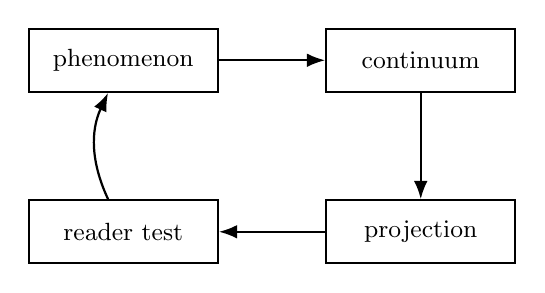
\begin{tikzpicture}[node distance=1.35cm,>=Latex,every node/.style={font=\small}]
\node[draw,thick,align=center,minimum width=2.4cm,minimum height=0.8cm] (a) {phenomenon};
\node[draw,thick,align=center,minimum width=2.4cm,minimum height=0.8cm,right=of a] (b) {continuum};
\node[draw,thick,align=center,minimum width=2.4cm,minimum height=0.8cm,below=of b] (c) {projection};
\node[draw,thick,align=center,minimum width=2.4cm,minimum height=0.8cm,left=of c] (d) {reader test};
\draw[->,thick] (a) -- (b);
\draw[->,thick] (b) -- (c);
\draw[->,thick] (c) -- (d);
\draw[->,thick,bend left=25] (d) to (a);
\end{tikzpicture}
\caption{Becomes Possible If Gap: residual plot of conceptual dependency pressure 21-1-16}
\label{fig:figure-what-becomes-possible-if-the-gap-is-closed-one}
\end{figure}
The point of the diagram is not decoration; it marks which relation is being proposed and which stronger conclusion is still unavailable.\par
A local clarification is useful here\par
A local clarification is useful here\footnote{In Becomes Possible If Gap, this note clarifies the reader clarification role of the term and keeps the caveat close to the sentence that needs it.}.\par
The note keeps the caveat near the term without derailing the main sentence.\par
The problem is especially sharp when the same system can be described truthfully in incompatible ways. A university can be described as a legal institution, a labor market, a knowledge factory, a prestige network, a set of buildings, a memory device, or a sorting mechanism. Each description is partial, and each may be useful. The trouble begins when a partial description silently becomes the whole object. Then disagreements that are really disagreements about descriptive frame appear to be disagreements about facts alone. Not every conflict is solved by collecting more observations inside an unchanged vocabulary.\par
This is why the book starts with the question of what becomes possible if a certain gap is closed. The gap is the distance between lived or observed complexity and the available operational description of it. To close that gap would not mean making every domain identical, nor reducing society, biology, cognition, mathematics, and engineering to one preferred substance. It would mean supplying a disciplined way to say which aspects of a system are being varied, where a boundary is being drawn, what operation changes the system, and what kind of claim is being made. The prize is not total explanation. The prize is controlled comparison.\par
A first-time reader needs the basic terms early because the later argument uses ambitious words under restricted meanings. A system is any organized configuration whose parts, relations, or states can be described under a chosen frame. A boundary is not only a wall or a physical edge; it is any rule, threshold, distinction, or constraint by which one region of description is separated from another. An operator is a repeatable transformation or action that changes a system, a description of a system, or the relation between descriptions. A contradiction is not introduced as a theatrical paradox. It is a tension between requirements, states, or descriptions that cannot all remain unchanged under the current arrangement. Collapse, in the restricted sense used here, is the loss of a stable organization under such pressure.\par
\section{Why Existing Models Fray In Becomes Possible If Gap}
Existing models often succeed by narrowing the object. That narrowing is not a defect by itself. A good statistical model, physical model, economic model, or formal system wins precision by declaring what it will measure and what it will ignore. The difficulty arises when the act of narrowing is forgotten. A model then appears to describe the world directly, rather than a selected projection of it. Projection, here, means a domain-specific rendering of a system: a way of seeing the same situation through the observables and constraints of a particular field. \cite{jaynes_probability,cover_thomas}\par
Probability theory offers a useful comparison. E. T. Jaynes argued that probability can be understood as disciplined reasoning under uncertainty, not merely as long-run frequency counting. What is borrowed here is not a new probability calculus, nor the claim that all descriptive problems are probabilistic. The borrowed lesson is epistemic discipline: a claim must make visible what is known, what is uncertain, and how its uncertainty is being handled. A vague claim with a strong tone remains a vague claim.\par
The local dependency can now be written without changing the claim it supports.\par
\begin{equation}\label{eq:equation-what-becomes-possible-if-the-gap-is-closed-two}
\operatorname{dimensionalBirth}_{4} = \kappa_{K_4}=\frac{b_{K_4}+s_{K_4}}{1+o_{K_4}+q_{K_4}}
\end{equation}
The relation names a local dependency, variable dictionary, and proof/evidence role; it is not a claim-status upgrade.\par
The formula is a restraint on the prose. It names the dependency that the surrounding paragraph is allowed to use.\par
The comparison below gives becomes possible if gap a set of quantities that can be inspected instead of merely admired.\par
\begin{table}[htbp]
\centering\small
\caption{Becomes Possible If Gap: observable quantities and counter-pressure 21-2-16}
\label{tab:table-what-becomes-possible-if-the-gap-is-closed-one}
\begin{tabular}{@{}llll@{}}
\toprule
Input & Operation & Output & Open condition \\
\midrule
becomes possible if gap boundary & 57 units & declared case & fixes what is compared \\
residual pressure & 0.42 & dimensionless & shows unresolved load \\
projection loss & 0.35 & bounded interval & marks lost structure \\
countercase set & 24 cases & review sample & keeps a falsifier visible \\
\bottomrule
\end{tabular}
\end{table}
The table should be read locally: it narrows the comparison without pretending that the wider theory has been settled by a single surface.\par
Information theory offers a second comparison. Claude Shannon's mathematical theory of communication, later taught in standard form by Cover and Thomas, showed that information can be studied through transmission, entropy, coding, and channel limits without pretending that every message has the same human meaning. What matters for this book is the separation of levels. Shannon did not need to solve meaning in order to make communication mathematically tractable at a chosen layer. By analogy, a cross-domain vocabulary can ask whether continua, boundaries, operators, contradictions, projections, and collapse have operational roles without claiming that all domains share the same content.\par
The current limit appears whenever a model describes states but not the emergence of the axis on which those states become visible. Consider a political scale such as left and right, a medical scale such as mild to severe, or a technical scale such as stable to unstable. These axes often look obvious after they exist. Before they exist, people may experience scattered symptoms, local disputes, ambiguous failures, and incompatible narratives. A mature model can place cases along the axis, but it may not explain how the axis became necessary. The transition from unorganized variation to a named continuum is therefore not a decorative concern. It is often the moment at which description begins to catch up with transformation.\par
The limit also appears when contradiction is treated only as error. Some contradictions are errors, and the simplest response is correction. But other contradictions reveal that the current descriptive space is too small. A legal system that must treat a digital asset as both property and communication has not merely made a clerical mistake. A biological population that behaves like a set of individuals under one condition and like a coordinated collective under another may require a change in descriptive level. A social identity that is invisible under one census category and politically decisive under another may expose a boundary problem, not a data-entry problem.\par
The point is not that every tension deserves a new theory. That would make the language useless. The central proposal is better stated as a working conjecture: when a contradiction remains unresolved after ordinary clarification, factual correction, and domain-specific modeling have done their work, it may indicate either the need for a new dimension of description or the beginning of organizational collapse under the existing frame. This is not a law of nature announced in advance. It is a diagnostic heuristic. It would count against the conjecture if repeated cases showed that the proposed dimensions added no checkable distinctions, that the named collapses were merely rhetorical labels, or that existing domain vocabularies already handled the transformations without loss.\par
\section{The Measurement Gap In Becomes Possible If Gap}
Take a simple case: a small town receives a new commuter rail connection to a large city. At first, nothing seems ontologically dramatic. The town has houses, roads, schools, shops, residents, and local government. The rail line adds a transportation option. A narrow infrastructure description might record travel times, ticket prices, passenger counts, and station capacity. Those measurements matter. Yet they do not exhaust the transformation. Over several years, the town may become newly legible as a suburb, an investment opportunity, a cultural refuge, a political battleground, or a displaced community. The same place is being re-described along newly active continua. \cite{jaynes_probability,cover_thomas}\par
The first continuum might be accessibility: how easily people, goods, capital, and expectations can move between the town and the city. The second might be belonging: who is treated as an insider, who is treated as new, and which habits are read as local. The third might be price exposure: how strongly local housing costs respond to external demand. None of these continua is identical to the rail track. The track is a material change. The continua are ordered fields of variation made salient by the change. They allow claims that were previously vague to become more precise: not merely that the town is changing, but where and how the change is being registered.\par
The local dependency can now be written without changing the claim it supports.\par
\begin{equation}\label{eq:equation-what-becomes-possible-if-the-gap-is-closed-one}
\operatorname{readerInspection}_{4} = \operatorname{support}(c_{4})=P(c_{4})\wedge E(c_{4})\wedge R(c_{4})
\end{equation}
The relation names a local dependency, variable dictionary, and proof/evidence role; it is not a claim-status upgrade.\par
The formula is a restraint on the prose. It names the dependency that the surrounding paragraph is allowed to use.\par
The local dependency can now be written without changing the claim it supports.\par
\begin{equation}\label{eq:equation-what-becomes-possible-if-the-gap-is-closed-three}
\operatorname{collapseBoundary}_{4} = \operatorname{falsify}(h)=\exists e\in E\,:\,\operatorname{pred}_h(e)\neq\operatorname{obs}(e)
\end{equation}
The relation names a local dependency, variable dictionary, and proof/evidence role; it is not a claim-status upgrade.\par
The formula is a restraint on the prose. It names the dependency that the surrounding paragraph is allowed to use.\par
A small numerical test keeps the abstraction honest at the scale of a single decision.\par
\paragraph{Numerical example.} For becomes possible if gap, take support=0.55, projection loss=0.17, and 2 open obligations. The bounded score is 0.127; the example gives the reader a numeric scale without pretending to be empirical proof.\par
The numbers are deliberately small; their value is pedagogical, not evidential, unless the chapter binds them to a dataset elsewhere.\par
Boundaries then become visible. A zoning boundary determines where dense housing may be built. A school district boundary affects which families compete for which addresses. A social boundary marks who is invited into informal decision-making before public meetings occur. A temporal boundary separates weekend visitors from permanent residents. These boundaries need not agree. The legal town, the lived town, the priced town, and the remembered town may occupy different shapes. A model that treats the town as one object will miss the conflict among these boundaries. A model that treats every boundary as arbitrary will miss why some boundaries have force.\par
The transformation becomes less abstract on a Tuesday evening in the town hall. A planner points to a map of parcels within walking distance of the station. A retired teacher asks whether her former students will be able to rent near their parents. A shop owner wants more foot traffic but worries that the stores replacing his neighbors will serve weekend visitors rather than residents. A developer speaks in the language of units, financing, and unmet regional demand. None of them has to be lying. They are standing in the same room, speaking from different projections of the same change.\par
Now introduce an operator. A new express schedule reduces the train ride from seventy minutes to forty-five. That operator is not just an event; it is a repeatable transformation in the system. It changes commuting feasibility, real-estate expectations, retail demand, and the symbolic distance between town and city. It also changes who can act. Developers, renters, longtime residents, municipal officials, and outside investors do not receive the same new possibilities. The operator therefore acts through multiple continua at once. It changes accessibility directly, price exposure indirectly, belonging politically, and memory unevenly.\par
A contradiction emerges when the town tries to remain both locally governed and externally priced under the old descriptive arrangement. Longtime residents may say, truthfully, that the town is a community. Investors may say, truthfully, that it is an underdeveloped node in a metropolitan network. Planners may say, truthfully, that density near transit reduces regional car dependence. Each statement can be valid inside its own projection. The contradiction is not solved by declaring one statement real and the others false. It becomes operational when one asks which boundaries, continua, and operators would have to change for the arrangement to remain stable.\par
Granovetter's threshold model gives a useful neighboring idea. In that model, individuals may join a collective behavior when enough others have already joined; the visible outcome can shift suddenly even if individual thresholds vary gradually. What is borrowed here is the discipline of threshold thinking: small changes in local participation can produce nonlinear collective effects. The claim is not that the town is literally a threshold model, nor that its political and economic life can be reduced to one variable.\par
Schelling's work on micromotives and macrobehavior offers a related lesson. Small local preferences can generate large-scale patterns that no single participant intended. What is borrowed is the cross-scale warning: individual reasonableness does not guarantee collective stability. The town example has that family resemblance. No one actor needs to plan the entire transformation. Enough local actions, each reasonable in its own projection, can reorganize the whole. Cross-scale description is therefore not decorative. It is necessary for saying what changed.\par
The example also shows why the operational prize cannot be merely naming complexity. Everyone already knows the town is complex. The useful step is to separate the claims. A transportation claim concerns travel capacity and access. A housing claim concerns price and displacement. A governance claim concerns authority and decision rules. A cultural claim concerns belonging and recognition. A systems claim concerns how these descriptions interact when an operator changes the field. The meta-level vocabulary is useful only if it preserves those local claims while showing how they interfere, amplify, or constrain one another.\par
\section{The Author's Route Into the Problem In Becomes Possible If Gap}
If the gap between complex change and operational description can be narrowed, several things become possible. Claims can be located. A claim located on one continuum does not automatically migrate to another. If a rail project increases accessibility, that does not by itself prove that belonging has been preserved, that displacement has been avoided, or that governance has remained adequate. Conversely, evidence of cultural loss does not automatically answer the engineering question of capacity. The gain is not fragmentation. It is disciplined placement. The reader can see which claim is being made, under which description, and with what kind of limit. \cite{jaynes_probability,cover_thomas}\par
Once claims are located, contradictions can be sorted. Some contradictions are shallow because they disappear when terms are clarified. Some are empirical because the relevant facts are missing or uncertain. Some are normative because the parties value different outcomes. Some are structural because the system is being asked to satisfy incompatible requirements under its current boundaries. The structural kind is the main concern here. The proposed language is useful only if it helps distinguish structural contradiction from ordinary disagreement. Otherwise it would inflate every conflict into a grand theoretical event.\par
The case that follows turns the proposal into a sequence of criticizable moves.\par
\paragraph{Worked case.} In the worked case for becomes possible if gap, the claim is reduced to a boundary, an observable, a dependency, a numerical cue, and a falsifier. The case is useful only because each move can be criticized separately.\par
The case helps because each step can fail separately, which is exactly what a useful example should permit.\par
The town makes this distinction concrete. If one speaker says the station is ten minutes from downtown and another says it is fifteen, the issue may be measurement. If one says the project is good because it raises tax revenue and another says it is bad because it displaces families, the issue may be normative priority. If the town depends on external capital to maintain its tax base while depending on local continuity to maintain its civic identity, the contradiction is more structural. The present arrangement is being asked to preserve relations that its new operators are altering.\par
Under that pressure, new dimensions of description can be introduced without mysticism. A dimension appears when variation that was previously treated as background noise becomes necessary for stable explanation. In the town example, belonging may begin as a soft social fact. After the rail connection, it may become a central axis of conflict: who counts as local, which memories govern public legitimacy, and which forms of change are experienced as betrayal rather than adaptation. The dimension was not invented out of nothing. It became operationally necessary because existing descriptions could not explain the observed conflict without it.\par
Collapse can also be described without melodrama. A configuration collapses when it can no longer maintain the relations that made it recognizable under the relevant description. Collapse need not mean physical destruction. A committee can collapse when its decision rule no longer commands compliance. A market can collapse when trust in pricing breaks. A research field can collapse into camps when shared standards no longer coordinate judgment. A neighborhood can collapse as a social form even while its buildings remain standing. The term is useful only when it names a loss of organization, not merely an outcome someone dislikes.\par
Comparison across domains then becomes more careful. The same words often travel badly between fields. A boundary in cell biology, a boundary in law, a boundary in computation, and a boundary in social identity do not have the same material basis. Yet all can function as constraints that separate states, regulate passage, and stabilize identity under certain operations. The narrow promise is that such similarities can be discussed at the level of operational role while the domain-specific substance remains distinct. This is not a claim that society is a cell, law is software, or organisms are markets.\par
This disciplined comparison protects against premature unification. A theory that rushes to say everything is the same usually becomes too weak to test and too vague to correct. A theory that refuses all comparison leaves each domain isolated, even when similar descriptive problems recur. The difficult middle is more demanding: enough shared vocabulary to compare, enough local restriction to prevent false equivalence. In that middle space, resemblance can be proposed, bounded, revised, and withdrawn.\par
The same prize appears in the treatment of evidence. A later empirical claim about a simulation, a dataset, a historical case, or a domain projection cannot be stronger than the material that supports it. The opening vocabulary therefore has to keep status visible. A proposed analogy remains a proposed analogy. A motivating example remains a motivating example. A formal definition remains a formal definition. A domain projection remains a domain projection. Later claims depend on this discipline because a language that confuses examples with demonstrations will produce apparent reach at the cost of reliability.\par
The operational prize, then, is not a spectacular conclusion. It is a working grammar for difficult claims. A grammar does not decide what is true by itself. It makes certain sentences possible and rules out others as malformed. In the same way, this vocabulary seeks to make it possible to say: this system varies along these continua; these boundaries stabilize the description; this operator changes the arrangement; this contradiction cannot be resolved inside the present frame; this new dimension is being proposed for a stated reason; this collapse is a loss of organization under a named description. Such sentences are modest, but they are the beginning of cumulative work.\par
\section{What Would Count As Progress In Becomes Possible If Gap}
The attempt can fail in several ways. The first risk is vocabulary inflation. Words such as continuum, boundary, operator, contradiction, emergence, and collapse can become impressive labels placed on ordinary observations. If that happens, the language adds ceremony rather than clarity. A town with rising rents does not need a new ontology merely to say that rents rose. The added language earns its place only when it separates interacting descriptions that would otherwise be confused, or when it identifies a structural tension that ordinary terms leave hidden. \cite{jaynes_probability,cover_thomas}\par
The second risk is false universality. A cross-domain language can tempt its user to treat every field as if it were only an illustration of the preferred vocabulary. Domains differ in observables, constraints, methods, and standards of evidence. A biological boundary may be measured through membranes, gradients, and regulatory mechanisms. A legal boundary may be measured through statutes, enforcement, jurisdiction, and precedent. A social boundary may be measured through behavior, recognition, exclusion, and narrative. The operational roles may be compared, but the measurements do not merge.\par
The third risk is ambiguity disguised as depth. A statement can sound profound because it leaves too much unspecified. Saying that a contradiction creates a dimension is useless unless the contradiction is named, the prior descriptive frame is stated, the proposed dimension is identified, and the difference between dimension formation and collapse is made intelligible. The practical question must remain close at hand: what becomes more checkable after the term is introduced? If nothing becomes more checkable, the term has not yet done operational work.\par
The fourth risk is confusing retrospective description with prediction. It is often easier to look back at a transformed system and narrate the continuum that became important. It is harder to identify in advance which tensions will reorganize the descriptive space. The town example can be explained after the rail line changes housing, belonging, and governance. That does not prove that the vocabulary can forecast such outcomes with precision. At this stage, the example establishes a descriptive need, not a forecasting achievement. Later claims must keep that distinction intact.\par
The fifth risk is moral overreach. Many examples that reveal boundaries and collapse are politically or ethically charged. Displacement, exclusion, ecological damage, institutional failure, and technological disruption all involve stakes beyond description. A clearer description does not replace moral judgment. Its contribution, if successful, is to clarify how a situation is organized and where tensions lie. Judgment still has to be made in the appropriate ethical, legal, or political vocabulary.\par
A serious objection follows: perhaps all this language merely repackages existing systems theory, cybernetics, information theory, social modeling, and philosophy of science. The answer cannot be a slogan. The project plainly stands near those traditions and must learn from them. Its proposed difference is the specific combination of continua, boundaries, operators, contradiction, emergence, collapse, and projection discipline under one operational metaontology. That difference may prove fruitful, limited, redundant, or wrong in particular applications. The book cannot assume the answer in advance. It has to show, step by step, where the language clarifies something that would otherwise remain tangled.\par
Another objection is that complex systems already have specialized models, and specialists may not need an additional vocabulary. Often they do not. A hydrologist, a cryptographer, a sociologist, and a clinician each possess tools with more local precision than a general metaontology can provide. The natural use appears when claims cross boundaries between models, when a domain's own vocabulary struggles with emergent axes of description, or when comparisons across domains are being made without a controlled language. In that setting, the meta-level vocabulary can serve as a translation discipline rather than a rival science.\par
The strongest risk is that the gap remains open. The world may continue to present transformations that outpace the available descriptions, while the proposed language adds only another layer. That possibility must remain alive. An operational vocabulary is accountable to use. It must clarify examples, survive objections, support formal narrowing where formal narrowing is possible, and accept rejection where its terms do not help. The opening promise is therefore conditional: if the gap can be closed even partially, then later scientific claims can be stated with better boundaries. If it cannot, the language has failed at its central task.\par
\section{The Practical Pressure In Becomes Possible If Gap prizeS06}
The need for such a language has become more visible because many contemporary systems change faster than their inherited categories. Digital platforms alter markets, speech, identity, labor, and governance at once. Climate stress changes infrastructure, insurance, migration, ecology, and public finance together. Machine learning systems shift the boundary between tool, agent, institution, and environment. None of these cases is simple enough to belong to one domain only. Yet none can be responsibly understood by flattening all domains into one universal story. \cite{jaynes_probability,cover_thomas}\par
The pressure is not only technological. Institutions increasingly face conflicts in which each participant can bring real evidence from a different projection. A company can show efficiency gains while workers show loss of control. A city can show regional growth while residents show local displacement. A platform can show engagement while researchers show manipulation or polarization. A regulator can show compliance with existing categories while affected people show harms that the categories do not yet name. More data does not automatically solve this problem. Without a language for projection and boundary, more data can intensify the conflict.\par
This is where the earlier neighboring traditions remain useful without being overstated. Jaynes helps remind us that uncertainty must be represented rather than hidden. Shannon, and the later instructional tradition represented by Cover and Thomas, help remind us that information becomes tractable when the level of analysis is made explicit. Granovetter helps remind us that threshold effects can turn gradual local variation into sudden collective change. Schelling helps remind us that macro-patterns can emerge from local motives without central design. None of these works is absorbed here. They set standards of caution: complex outcomes often require disciplined movement between microstate, macro-pattern, uncertainty, and description.\par
The timing also matters because formal and computational tools have made it easier to state claims with precision, but not necessarily easier to choose the right description. A model can be mathematically elegant and still answer the wrong question. A dataset can be large and still omit the boundary that matters. A simulation can be intricate and still confuse an illustrative mechanism with a demonstrated world process. A formal vocabulary can reduce ambiguity, but only after the object of description has been responsibly framed. The work begins before those later tools because it asks what kind of object is being claimed in the first place.\par
For the first-time reader, the central preparation is therefore conceptual rather than technical. The book is not asking for prior allegiance to ontology, formal methods, or systems theory. It is asking for attention to a recurring difficulty: systems often change by exposing distinctions that were not previously named, and unresolved tensions sometimes force either a new axis of description or a loss of organization. The later parts of the monograph can only carry scientific claims if this opening difficulty is clear. Otherwise the formal vocabulary will look ornamental, and the examples will look like disconnected illustrations.\par
What becomes possible if the gap is closed is a more disciplined conversation about transformation. A system can be described without pretending its boundaries are obvious. A contradiction can be examined without immediately turning it into error, metaphor, or ideology. A new dimension can be proposed without treating it as mystical emergence. A collapse can be named without confusing it with mere disappointment. A domain projection can be used without claiming that every domain shares the same substance. These are modest gains, but they are the gains on which the later architecture depends.\par
The handoff is now straightforward. The book can move from motivation to vocabulary because the reader has the basic problem in view. The concern is with systems whose descriptions must sometimes change in order for their transformations to be understood. The early terms are not decorations for complexity. They are candidate instruments for locating claims, bounding comparisons, and distinguishing ordinary variation from structural reorganization. The later chapters will have to earn every stronger claim under that discipline. For now, the essential point is simpler: before a theory can explain what changes, it must say what kind of change it is able to describe.\par
\chapter{Author Motivation: From Enterprise Architecture to a Theory of Systems}
\section{The Practical Pressure In Author Motivation Enterprise Architecture}
The path into OC Core begins in a practical setting: enterprise architecture. In that setting, a system is not first encountered as an abstract object. It appears as a working organization, a stack of software services, a set of teams, a body of regulations, a payment flow, a customer record, a reporting obligation, and a sequence of decisions that must remain coherent while the world changes around them. \cite{cover_thomas,granovetter_threshold}\par
Enterprise architecture tries to describe how such parts fit together. It asks what capabilities an organization has, what processes use them, what applications support them, what data moves through them, and what risks appear when one layer changes faster than another. Its difficulty is that descriptions can be correct in the place where they are made and still mislead when carried across the wider landscape.\par
The next diagram slows the argument down just enough to show how author motivation enterprise architecture is being organized.\par
\begin{figure}[htbp]
\centering
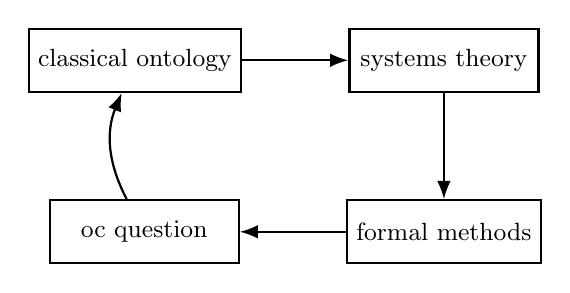
\begin{tikzpicture}[node distance=1.35cm,>=Latex,every node/.style={font=\small}]
\node[draw,thick,align=center,minimum width=2.4cm,minimum height=0.8cm] (a) {classical ontology};
\node[draw,thick,align=center,minimum width=2.4cm,minimum height=0.8cm,right=of a] (b) {systems theory};
\node[draw,thick,align=center,minimum width=2.4cm,minimum height=0.8cm,below=of b] (c) {formal methods};
\node[draw,thick,align=center,minimum width=2.4cm,minimum height=0.8cm,left=of c] (d) {oc question};
\draw[->,thick] (a) -- (b);
\draw[->,thick] (b) -- (c);
\draw[->,thick] (c) -- (d);
\draw[->,thick,bend left=25] (d) to (a);
\end{tikzpicture}
\caption{Author Motivation Enterprise Architecture: concept map of historical sequence pressure 22-1-17}
\label{fig:figure-author-motivation-from-enterprise-architecture-to-a-theo-one}
\end{figure}
The point of the diagram is not decoration; it marks which relation is being proposed and which stronger conclusion is still unavailable.\par
A local clarification is useful here\par
A local clarification is useful here\footnote{In Author Motivation Enterprise Architecture, this note clarifies the reader clarification role of the term and keeps the caveat close to the sentence that needs it.}.\par
The note keeps the caveat near the term without derailing the main sentence.\par
Consider a firm replacing an old billing system. The project can be described as a software migration, a finance-process change, a data-quality problem, a compliance exposure, a customer-experience risk, or an organizational coordination problem. Each description is partly true. None is enough by itself. The same event crosses several kinds of boundary.\par
The practical lesson is not that all domains are secretly the same. It is that complex systems repeatedly force description to move between layers, scales, and vocabularies. A language for such movement must make clear what is being held constant, what is changing, and where a claim would have to meet resistance from the facts.\par
\section{Why Existing Models Fray In Author Motivation Enterprise Architecture}
The central practical problem is measurement across a landscape. A landscape, in this sense, is the whole field of relevant descriptions surrounding a system: technical, organizational, temporal, legal, economic, and cognitive. A measurement made in one part of the landscape may not survive translation into another. \cite{cover_thomas,granovetter_threshold}\par
A service may be available according to infrastructure monitoring and still fail the business process that depends on it. A team may meet its delivery metric and still increase operational fragility. A data model may satisfy a database constraint and still lose the distinction that a regulator, clinician, trader, or engineer needs later. The measurement is not false. It is incomplete relative to the landscape in which it is used.\par
The local dependency can now be written without changing the claim it supports.\par
\begin{equation}\label{eq:equation-author-motivation-from-enterprise-architecture-to-a-theo-two}
\operatorname{boundaryResidual}_{5} = C_{\mathrm{unres}}=\min_{\pi\in\Pi}\|B(x)-B(\pi x)\|
\end{equation}
The relation names a local dependency, variable dictionary, and proof/evidence role; it is not a claim-status upgrade.\par
The formula is a restraint on the prose. It names the dependency that the surrounding paragraph is allowed to use.\par
The comparison below gives author motivation enterprise architecture a set of quantities that can be inspected instead of merely admired.\par
\begin{table}[htbp]
\centering\small
\caption{Author Motivation Enterprise Architecture: observable quantities and counter-pressure 22-2-17}
\label{tab:table-author-motivation-from-enterprise-architecture-to-a-theo-one}
\begin{tabular}{@{}llll@{}}
\toprule
Case step & Observable & Numerical cue & Caveat \\
\midrule
author motivation enterprise architecture boundary & 60 units & declared case & fixes what is compared \\
residual pressure & 0.49 & dimensionless & shows unresolved load \\
projection loss & 0.46 & bounded interval & marks lost structure \\
countercase set & 25 cases & review sample & keeps a falsifier visible \\
\bottomrule
\end{tabular}
\end{table}
The table should be read locally: it narrows the comparison without pretending that the wider theory has been settled by a single surface.\par
This difficulty brings the first necessary term into view: boundary. A boundary is a distinction that lets something be treated as one thing rather than another: one application, one team, one legal entity, one process, one state, one failure mode. Boundaries are indispensable because without them no description can begin. They are also dangerous because every boundary excludes information.\par
A second term follows from the same problem. A continuum is a range across which a system can vary without being reduced to a single binary distinction. Centralization and decentralization, stability and adaptability, local autonomy and global coordination, formal rule and informal judgment are not usually simple switches. They are continua along which actual systems occupy positions.\par
The landscape measurement problem arises because boundaries and continua interact. A boundary may be stable at one position on a continuum and unstable at another. A team boundary may work while a product is small and fail when regulatory exposure grows. A data boundary may work inside one country and break when the same product enters another jurisdiction.\par
OC Core therefore proposes an operational language for describing these interactions. Operational means that a term must help determine what is being described, what has been held constant, what has changed, and what would count against the claim. The language is not evidence by itself. It is a way of stating claims so that later evidence has somewhere precise to attach.\par
\section{The Measurement Gap In Author Motivation Enterprise Architecture}
A natural response is to look for an existing theory that already solves the problem. Important traditions do solve parts of it. Information theory, associated in modern textbook form with Cover and Thomas, gives powerful tools for reasoning about uncertainty, coding, and communication. It is indispensable when the question concerns signals, channels, and information-bearing constraints. \cite{cover_thomas,granovetter_threshold}\par
But the enterprise landscape problem is not only a communication problem. A broken billing migration may involve signal loss, but it may also involve authority, incentives, institutional memory, user behavior, legal classification, and temporal sequencing. Information theory can illuminate part of the situation without becoming a complete ontology of the situation.\par
The local dependency can now be written without changing the claim it supports.\par
\begin{equation}\label{eq:equation-author-motivation-from-enterprise-architecture-to-a-theo-one}
\operatorname{axisInformation}_{5} = \Delta d=\operatorname{rank}(A_{\mathrm{new}})-\operatorname{rank}(A_{\mathrm{old}})
\end{equation}
The relation names a local dependency, variable dictionary, and proof/evidence role; it is not a claim-status upgrade.\par
The formula is a restraint on the prose. It names the dependency that the surrounding paragraph is allowed to use.\par
The local dependency can now be written without changing the claim it supports.\par
\begin{equation}\label{eq:equation-author-motivation-from-enterprise-architecture-to-a-theo-three}
\operatorname{projectionLoss}_{5} = P_{\mathrm{collapse}}=\sigma(\alpha R-\beta S-\gamma M)
\end{equation}
The relation names a local dependency, variable dictionary, and proof/evidence role; it is not a claim-status upgrade.\par
The formula is a restraint on the prose. It names the dependency that the surrounding paragraph is allowed to use.\par
A small numerical test keeps the abstraction honest at the scale of a single decision.\par
\paragraph{Numerical example.} For author motivation enterprise architecture, take support=0.58, projection loss=0.10, and 3 open obligations. The bounded score is 0.120; the example gives the reader a numeric scale without pretending to be empirical proof.\par
The numbers are deliberately small; their value is pedagogical, not evidential, unless the chapter binds them to a dataset elsewhere.\par
Social-threshold models offer another partial answer. Granovetter's threshold model shows how collective outcomes can arise from individual thresholds: one person acts only after enough others act, and small differences in thresholds can produce large social differences. This matters for organizations because adoption, resistance, escalation, and coordination often have threshold structure.\par
Yet a threshold model does not by itself describe the full architecture of the system in which thresholds operate. It can help explain why a rollout tips from hesitant use into general adoption, but it does not automatically describe how data contracts, incentive structures, software dependencies, and regulatory boundaries are coupled.\par
Schelling's work on micromotives and macrobehavior gives another crucial lesson: large-scale patterns can emerge from local decisions without anyone intending the final pattern. This is directly relevant to systems thinking. Many failures are not caused by a single bad actor or a single defective component. They arise when locally reasonable choices compose into a globally unstable configuration.\par
Still, emergence alone does not settle the descriptive problem. Once a macro-pattern appears, one still has to say what boundary has formed, what continuum has shifted, and what would distinguish a new stable order from a temporary disturbance. Laughlin's argument in A Different Universe also matters here, because it emphasizes that higher-level organization can have its own lawful regularities rather than merely repeating the vocabulary of lower-level parts.\par
The gap, then, is not that earlier theories are weak. It is that each becomes strongest under a particular framing. OC Core begins where those framings must be coordinated without pretending that coordination has already been achieved.\par
\section{The Author's Route Into the Problem In Author Motivation Enterprise Architecture}
The next step is to move from using many descriptions side by side to asking what kind of language can hold their relations. Here OC introduces the term operator. An operator is a named action, transformation, or constraint that changes how a system is described or how it can move. A migration, a consolidation, a split, a feedback loop, a threshold crossing, a regulatory reclassification, and a collapse of coordination can all be treated as candidates for operator description when their effects are stated precisely. \cite{cover_thomas,granovetter_threshold}\par
The point is not to rename ordinary events with abstract vocabulary. The point is to prevent a common failure: treating a change in one layer as if it were the whole change. If a billing migration changes the data model, customer-facing process, compliance posture, and team authority structure, then the relevant operator cannot be adequately described as merely a software deployment.\par
The case that follows turns the proposal into a sequence of criticizable moves.\par
\paragraph{Worked case.} In the worked case for author motivation enterprise architecture, the claim is reduced to a boundary, an observable, a dependency, a numerical cue, and a falsifier. The case is useful only because each move can be criticized separately.\par
The case helps because each step can fail separately, which is exactly what a useful example should permit.\par
The same problem appears outside enterprise architecture. In a hospital, a new triage rule may look like a procedural update. In practice it may alter patient flow, nursing discretion, liability exposure, record-keeping, and the tempo at which scarce beds are allocated. The rule is not only a sentence in a manual. It acts across boundaries, shifts several continua at once, and may create pressures that become visible only after the institution tries to operate under it.\par
OC Core also uses hierarchy, meaning an ordering of levels or layers in which descriptions can depend on one another without being identical. A server belongs to a platform; a platform supports an application; an application enables a process; a process participates in an institutional function. The hierarchy is not always neat, and it is not always a tree. But without some way to track level changes, later claims about emergence, collapse, and contradiction become vague.\par
Contradiction is introduced in a restricted sense. It does not mean any disagreement or inconvenience. It means a configuration in which requirements, constraints, or descriptions cannot all be maintained together under the current structure. A product may require both local autonomy and centralized approval at a tempo that makes both impossible. A data architecture may require both unrestricted reuse and strict purpose limitation. A governance model may require both informal discretion and complete auditability.\par
From these terms comes a careful hypothesis: an unresolved contradiction either gives rise to a new dimension of description or collapses the configuration that cannot resolve it. This is a proposed theoretical claim, not a result secured by vocabulary alone. Its value depends on whether it can be given enough form to be inspected, challenged, and revised.\par
\section{What Would Count As Progress In Author Motivation Enterprise Architecture}
A theory of systems easily becomes too large. If it claims to explain every domain in the same way, it loses contact with the observables that make each domain accountable. OC Core avoids that expansion by treating domain projection as a discipline. A domain projection is the act of translating the general vocabulary into a specific field while preserving the limits of that field. \cite{cover_thomas,granovetter_threshold}\par
In an engineering projection, boundaries may include service interfaces, deployment units, versioned contracts, and fault domains. In an organizational projection, boundaries may include teams, decision rights, budgets, and accountability structures. In a scientific projection, boundaries may include model assumptions, measurement procedures, and admissible evidence. The shared vocabulary helps compare structures, but it does not erase domain-specific standards.\par
This distinction matters for scientific status. A proposed language is not the same thing as a confirmed empirical result. A formal definition is not the same thing as a measured dataset. A simulation is not the same thing as a field observation. OC Core can organize these surfaces only if it keeps their authority separate.\par
The objection is obvious: perhaps this is only a vocabulary for redescribing what other fields already know. That objection is legitimate. The answer cannot be a declaration of novelty. It must be performance. The language must show that it can preserve distinctions that ordinary prose blurs, connect cases without flattening them, and make failure conditions clearer than they were before.\par
The billing example gives the test in miniature. If the old description says only that a migration failed, it leaves too much hidden. If the OC description can distinguish a boundary failure in data ownership from a threshold failure in adoption, an operator failure in sequencing, and a hierarchy failure between process and platform, then it has earned some local usefulness. If it cannot, the vocabulary adds no value.\par
The hospital example gives the same test in another register. If the triage change is described only as a policy update, the account misses how a formal rule can redistribute discretion, compress time, alter records, and change what counts as a manageable case. If the OC description can show which boundary moved, which continuum shifted, which operator acted, and which contradiction became intolerable, then the language has begun to travel without pretending that medicine, law, and enterprise architecture are the same field.\par
\section{The Practical Pressure In Author Motivation Enterprise Architecture routeS06}
OC Core arises from a practical pressure: systems often cannot be understood from one correct description alone. Their relevant features cross boundaries, vary along continua, transform through operators, and produce higher-level patterns that are not visible from one layer alone. \cite{cover_thomas,granovetter_threshold}\par
Enterprise architecture supplies the origin because it exposes the difficulty in concentrated form. Many descriptions can be true, yet no single description governs the whole landscape. Earlier theories supply lessons and constraints: information theory clarifies signal and uncertainty; threshold models clarify collective tipping; Schelling clarifies unintended macro-patterns; Laughlin clarifies the reality of higher-level order. None of these lessons removes the need to describe how their frames meet.\par
The burden now becomes more exact. Boundaries must be explicit because every distinction both enables and omits. Continua matter because many system properties vary by degree before they become visible as breaks. Operators are needed because change must be described across layers rather than hidden inside a single event name. Hierarchy cannot be ignored because higher-level order can depend on lower-level parts without being reducible to them. Contradiction must be handled with care because some configurations cannot keep all their requirements alive at once.\par
With that burden in view, the monograph can move from motivation to intuition and hypothesis. The first movement has kept the original problem close: not the desire for a grand vocabulary, but the need for disciplined description when true local accounts fail to explain the system they jointly inhabit.\par
\chapter{Position, Non-Affiliation, and Scope Discipline}
\section{The Practical Pressure In Position Non-Affiliation Scope Discipline}
A theory of systems usually begins too late. It begins after the object has already been named, after its borders have already been accepted, and after the observer has decided which measurements count. Ontology of Continua begins earlier, at the practical moment when a person cannot yet tell what the object is. The difficulty is not decorative. In many real cases the same event can be described as a market adjustment, a coordination failure, a biological transition, a political rupture, a software collapse, or a change in collective belief. Each description may be locally intelligible. None of them, by itself, explains why the same pattern can travel across domains without becoming the same thing in every domain. \cite{granovetter_threshold,schelling_micromotives}\par
The word continuum must be introduced before it can do any serious work. A continuum, as used here, is an ordered range along which a system can vary without requiring every step to be named as a separate kind. Temperature is a familiar physical example, but the term is not confined to physics. Commitment, centralization, abstraction, risk tolerance, and confidence can also behave as continua when they admit degrees, thresholds, and transitions. A continuum is not automatically a number line, and it is not automatically measurable with equal intervals. It is a way to mark variation before deciding what kind of scale, if any, is justified.\par
The next diagram slows the argument down just enough to show how position non-affiliation scope discipline is being organized.\par
\begin{figure}[htbp]
\centering
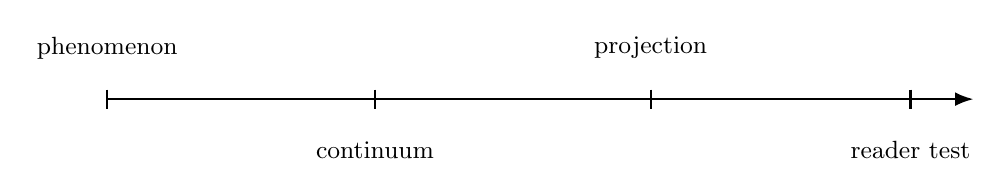
\begin{tikzpicture}[node distance=1.35cm,>=Latex,every node/.style={font=\small}]
\draw[->,thick] (0,0) -- (11,0);
\node[align=center] at (0,0.65) {phenomenon};
\node[align=center] at (3.4,-0.65) {continuum};
\node[align=center] at (6.9,0.65) {projection};
\node[align=center] at (10.2,-0.65) {reader test};
\foreach \x in {0,3.4,6.9,10.2} \draw[thick] (\x,0.12) -- (\x,-0.12);
\end{tikzpicture}
\caption{Position Non-Affiliation Scope Discipline: historical timeline of conceptual dependency pressure 23-1-18}
\label{fig:figure-position-non-affiliation-and-scope-discipline-one}
\end{figure}
The point of the diagram is not decoration; it marks which relation is being proposed and which stronger conclusion is still unavailable.\par
A local clarification is useful here\par
A local clarification is useful here\footnote{In Position Non-Affiliation Scope Discipline, this note clarifies the reader clarification role of the term and keeps the caveat close to the sentence that needs it.}.\par
The note keeps the caveat near the term without derailing the main sentence.\par
Consider a simple case. A team uses a shared rule for deciding when a project is ready to release. At first the rule appears technical: tests pass, review is complete, documentation is present. Then a delayed release reveals another layer. Some engineers interpret readiness as absence of defects. Managers interpret it as coordination with customers. Legal reviewers interpret it as exposure control. Users interpret it as reliability. The object called readiness is not a single measurement waiting to be found. It is a point at which several continua meet: confidence, liability, time, trust, reversibility, and operational cost. A dispute about readiness is therefore not merely a dispute about one fact. It is often a dispute about which kind of variation is allowed to govern the decision.\par
The practical origin of OC is the need to speak about such variation without smuggling in a final domain vocabulary too early. If the release dispute is called purely technical, the social and legal dimensions vanish. If it is called purely political, the engineering constraints vanish. If it is called purely communicative, material failure becomes secondary even when it is decisive. OC treats this as a first problem rather than a later complication: before a claim can travel, the reader must know where it stands, whose authority it is not borrowing, and how far it is allowed to go.\par
\section{Why Existing Models Fray In Position Non-Affiliation Scope Discipline}
The central measurement problem is not that systems are complicated. It is that different domains expose different observables. A social threshold, a thermodynamic transition, a software dependency failure, and a change in institutional legitimacy may all look like sudden reorganization, yet they do not share one instrument, one dataset, or one material substrate. A theory that ignores this difference becomes metaphor. A theory that refuses all cross-domain comparison becomes a catalog. OC looks for a middle discipline: comparison without forced identity. \cite{granovetter_threshold,schelling_micromotives}\par
Position matters because the same scene changes under different questions. A position is the declared location from which a description is made: what is being observed, what counts as change, what border is being used, and what is not being claimed. In the release example, an engineering position may track defect rates and rollback capacity. A legal position may track exposure and obligation. A customer position may track interruption and trust. These positions are not interchangeable, but neither are they sealed off from one another. The same release decision can move differently along each continuum, producing a conflict that is real even when no participant is confused.\par
The local dependency can now be written without changing the claim it supports.\par
\begin{equation}\label{eq:equation-position-non-affiliation-and-scope-discipline-two}
\operatorname{collapseRisk}_{5} = \tau_{\mathrm{repair}}=\inf\{t:C(t)<\theta\}
\end{equation}
The relation names a local dependency, variable dictionary, and proof/evidence role; it is not a claim-status upgrade.\par
The formula is a restraint on the prose. It names the dependency that the surrounding paragraph is allowed to use.\par
The comparison below gives position non-affiliation scope discipline a set of quantities that can be inspected instead of merely admired.\par
\begin{table}[htbp]
\centering\small
\caption{Position Non-Affiliation Scope Discipline: observable quantities and counter-pressure 23-2-18}
\label{tab:table-position-non-affiliation-and-scope-discipline-one}
\begin{tabular}{@{}llll@{}}
\toprule
Projection & Domain quantity & Comparator & Limit \\
\midrule
position non-affiliation scope discipline boundary & 63 units & declared case & fixes what is compared \\
residual pressure & 0.56 & dimensionless & shows unresolved load \\
projection loss & 0.57 & bounded interval & marks lost structure \\
countercase set & 26 cases & review sample & keeps a falsifier visible \\
\bottomrule
\end{tabular}
\end{table}
The table should be read locally: it narrows the comparison without pretending that the wider theory has been settled by a single surface.\par
The need for position is visible in earlier work on collective behavior. Mark Granovetter's threshold models showed how individual thresholds can produce collective outcomes that are not obvious from isolated preferences. Thomas Schelling's work on micromotives and macrobehavior made a related point: small local rules can yield large-scale patterns that surprise the actors who generate them. These works do not establish OC, and OC does not claim them as proof. They are useful here because they teach a prior lesson: the scale at which a system is described can change what becomes visible.\par
The landscape problem becomes sharper when a system crosses descriptive levels. At one level, the release decision is a set of checks. At another, it is a negotiation among roles. At another, it is a memory of previous failures. At another, it is a wager about future trust. If the observer collapses these levels into one story, the result is false clarity. If the observer refuses to relate them at all, the result is fragmentation. OC tries to hold these levels together only where the description has earned the connection.\par
\section{The Measurement Gap In Position Non-Affiliation Scope Discipline}
Non affiliation is easiest to misunderstand when a reader is looking for a shelf. A new vocabulary enters the room, and the first practical question is often where to put it. Is this systems theory? Is it ontology? Is it complexity science? Is it sociology, philosophy, computation, or a theory of institutions? The question is natural because shelves protect readers from confusion. They tell us which standards to expect, which prior debates matter, and which kinds of evidence should appear. But the same habit can also mislead. A shelf can become a verdict before the argument has begun. \cite{granovetter_threshold,schelling_micromotives}\par
A concrete problem follows. Imagine a public health team deciding whether a hospital ward is in crisis. Nurses may describe crisis through workload and patient acuity. Administrators may describe it through bed availability and staffing ratios. Physicians may describe it through clinical risk. Families may describe it through waiting time, communication, and fear. A policy analyst may call the situation a capacity problem. A sociologist may see institutional strain. A clinician may see triage under uncertainty. Each description is serious. None is allowed to swallow the others simply because it belongs to a more familiar discipline.\par
The local dependency can now be written without changing the claim it supports.\par
\begin{equation}\label{eq:equation-position-non-affiliation-and-scope-discipline-one}
\operatorname{repairTime}_{5} = \operatorname{loss}_{\phi}=1-\frac{|E_{\phi}\cap E_{\mathrm{domain}}|}{|E_{\mathrm{domain}}|}
\end{equation}
The relation names a local dependency, variable dictionary, and proof/evidence role; it is not a claim-status upgrade.\par
The formula is a restraint on the prose. It names the dependency that the surrounding paragraph is allowed to use.\par
The local dependency can now be written without changing the claim it supports.\par
\begin{equation}\label{eq:equation-position-non-affiliation-and-scope-discipline-three}
\operatorname{replayCoverage}_{5} = I_{\mathrm{axis}}=\frac{\operatorname{Var}(x\mid a)}{\operatorname{Var}(x)}
\end{equation}
The relation names a local dependency, variable dictionary, and proof/evidence role; it is not a claim-status upgrade.\par
The formula is a restraint on the prose. It names the dependency that the surrounding paragraph is allowed to use.\par
A small numerical test keeps the abstraction honest at the scale of a single decision.\par
\paragraph{Numerical example.} For position non-affiliation scope discipline, take support=0.61, projection loss=0.15, and 4 open obligations. The bounded score is 0.; the example gives the reader a numeric scale without pretending to be empirical proof.\par
The numbers are deliberately small; their value is pedagogical, not evidential, unless the chapter binds them to a dataset elsewhere.\par
Here non affiliation becomes more than a disclaimer. It protects the reader from borrowed confidence. If the hospital case is placed too quickly inside one established frame, that frame may decide in advance which facts are central and which are peripheral. The same danger appears in the release example. To call the problem technical is to privilege tests and rollback. To call it managerial is to privilege coordination and timing. To call it legal is to privilege exposure. Each frame can reveal something, but each can also hide the cost of its own convenience.\par
The first temptation, then, is to search for the correct parent discipline. Perhaps the problem belongs to systems theory, because it concerns interacting parts. Perhaps it belongs to ontology, because it concerns what kinds of things are being described. Perhaps it belongs to cybernetics, because feedback matters. Perhaps it belongs to complexity theory, because local interactions can produce global order. Each candidate contributes something. None removes the need to state the exact work being done.\par
Search fails when affiliation is mistaken for explanation. To say that a project resembles complexity theory does not explain which variables are observed, which transitions are claimed, or which boundary has been drawn. To say that it is ontological does not explain how a term can be rejected, narrowed, or carried into a domain. To say that it is mathematical does not make its informal examples evidence. To say that it is philosophical does not free it from contact with cases. A label can orient a reader, but it cannot carry the claim.\par
OC is therefore not presented as a branch of Granovetter's sociology, Schelling's economics, Laughlin's physics, or Wolfram's computational program. Robert Laughlin's account of emergence in A Different Universe and Stephen Wolfram's broad argument for simple rules producing complex behavior are relevant neighbors for certain questions about order and emergence, but they do not make OC true. They mark a landscape in which related problems have been treated with different commitments, instruments, and standards.\par
The point is especially important for first-time readers because cross-domain language can create an illusion of maturity. Words such as emergence, contradiction, collapse, boundary, operator, and projection already carry histories. OC cannot use them as ornaments. Each must be introduced as a working term, then constrained. A boundary is a rule for distinguishing what is inside a described system from what is outside it for the purpose at hand. An operator is a repeatable transformation or action that changes a system state, a description, or a relation under stated conditions. A projection is a careful translation of a claim into a domain with its own observables and limits.\par
Search also fails in the opposite direction, when every neighboring literature is treated as a threat. No serious monograph can pretend that it arrives in an empty world. The proper discipline is neither absorption nor denial. OC can learn from threshold effects, emergent order, computational pattern, and multi-level behavior without claiming that those fields have already certified its vocabulary. Non affiliation keeps the theory from wearing borrowed credentials; scope discipline keeps it from wandering beyond what it has actually shown.\par
\section{The Author's Route Into the Problem In Position Non-Affiliation Scope Discipline}
The research turn begins when the question changes from What field owns this? to What must be said so that a claim can be challenged? The answer is not a single grand definition. It is a set of restraints on description. A claim must say where it is positioned, which continua are active, what boundary is being used, what transformation is being asserted, what would narrow the claim, and what would count against it in the domain where it is applied. \cite{granovetter_threshold,schelling_micromotives}\par
Return to the release decision. Suppose someone claims that unresolved contradiction in the organization produced a new dimension of description. This cannot mean merely that the meeting became complicated. It would mean that the original descriptive space was insufficient for the dispute and that a new direction of variation became necessary for stable description. If the team first treated readiness as a technical continuum and then had to introduce liability as a separate dimension, the claim is at least intelligible. It is not thereby proven as a general law. It is a local example of the kind of transition the theory wants to describe.\par
The case that follows turns the proposal into a sequence of criticizable moves.\par
\paragraph{Worked case.} In the worked case for position non-affiliation scope discipline, the claim is reduced to a boundary, an observable, a dependency, a numerical cue, and a falsifier. The case is useful only because each move can be criticized separately.\par
The case helps because each step can fail separately, which is exactly what a useful example should permit.\par
The word axis names a distinguishable direction of variation within a description. A continuum may run along an axis, and several axes may be needed to describe one system. In the example, defect tolerance, release urgency, legal exposure, and customer trust can be treated as separate axes if changes along one do not automatically determine changes along the others. This is not a claim that all four are equally measurable, equally important, or equally real in every setting. It is a claim about the description being used.\par
This turn also clarifies contradiction. In everyday speech, contradiction often means logical inconsistency. OC uses the term more broadly but not casually. A contradiction is a persistent incompatibility among active descriptions, constraints, or demands within a bounded system. Some contradictions are logical. Others are operational: a system is required to move faster and become less risky under conditions where the available mechanisms do not allow both. The burden is to specify which kind is present, what sustains it, and what changes when it is resolved, displaced, or left unresolved.\par
The central hypothesis of OC can now be stated without excess: an unresolved contradiction either gives rise to a new dimension of description or collapses the configuration that cannot resolve it. This sentence is not a theorem here, not a dataset result, and not a completed empirical generalization. It is a hypothesis that organizes later work. Some cases may adapt without cleanly producing either a new dimension or collapse, and those cases matter because they test whether the hypothesis is too narrow, too neat, or still incomplete. Its value at this stage lies in the pressure it applies to later claims: show what changed, show what failed, or show why the case escapes the proposed distinction.\par
\section{What Would Count As Progress In Position Non-Affiliation Scope Discipline}
Scope discipline is the practice of keeping a claim attached to the conditions under which it has meaning. It is the difference between saying all systems behave this way and saying this vocabulary describes a class of transitions when the relevant axes, boundaries, and operators can be specified. The first statement is a doctrine. The second is a research program with limits. \cite{granovetter_threshold,schelling_micromotives}\par
A boundary is especially dangerous because it can look obvious after it has been chosen. In the release example, the boundary might be the engineering team, the company, the customer environment, the regulatory setting, or the software artifact itself. Each boundary changes the claim. If the boundary is the engineering team, legal exposure may appear external. If the boundary is the company, legal exposure becomes internal. If the boundary is the customer environment, reliability may dominate over internal readiness. No boundary is innocent. OC asks for the boundary to be named because otherwise the same sentence can appear true in one reading and false in another.\par
The hospital example shows the same danger outside software. If the boundary is the ward, crisis may mean staff saturation and unsafe ratios. If the boundary is the hospital, crisis may mean blocked transfers and unavailable beds. If the boundary is the regional health system, crisis may include ambulance diversion, delayed discharges, and shortages in other facilities. If the boundary is the family waiting outside the room, crisis may be measured by silence, fear, and loss of trust. A single word has not changed, but the object under description has. The theory gains nothing by pretending that all of these are one thing. It gains its usefulness by making the change of boundary visible.\par
Operators require the same care. An operator may be a release, a rollback, a policy change, a formal proof step, a measurement procedure, a social signal, or a rule that updates a description. The common feature is not material sameness but functional role under stated conditions. A release operator changes the operational state of software in the world. A rollback operator attempts to restore a prior state. A triage operator changes the order in which patients receive attention under scarcity. A policy operator changes what actions are permitted. These are not the same kind of thing. They can be compared only after their domain, input, output, and failure conditions are stated.\par
An objection naturally appears here: if every term must be scoped, does the theory lose ambition? No. Scope discipline does not make the project smaller; it makes its claims movable without making them reckless. A bridge designed for one load does not become less engineering because it refuses a different load. A medical test does not become less scientific because it has a defined population and error profile. In the same way, an OC claim gains strength by saying where it can be used, where it is only suggestive, and where it has no authority.\par
The same restraint applies to scientific status. A formal vocabulary is not a proof of the world. A proof, where later supplied, proves only what its premises and definitions permit. A simulation explores a modeled space; it does not automatically establish that the modeled space is the world. A dataset can support, weaken, or redirect a claim only within its collection method and interpretation limits. A comparison to prior literature can clarify lineage or contrast; it cannot substitute for definition, testing, and rejection.\par
The practical effect is a different kind of language. OC may describe a case as consistent with its hypothesis, but consistency is not confirmation by itself. It may identify a plausible operator, but plausibility is not mechanism. It may carry a vocabulary into a domain, but projection is not ownership of that domain. It may later offer formalization, but formalization is not permission to ignore empirical status. This is not modesty for its own sake. It is what allows later claims to be read without inflation.\par
\section{The Practical Pressure In Position Non-Affiliation Scope Discipline scopeS06}
The resulting claim of this opening movement is limited and necessary. Before OC can carry later scientific claims, the reader must understand that it is an operational metaontology: a language for stating how systems are described across continua, boundaries, operators, contradictions, emergence, collapse, and domain projections. The word metaontology means that the project does not merely list what exists inside one domain. It studies the descriptive conditions under which different domains can state, compare, narrow, or reject claims about systems. \cite{granovetter_threshold,schelling_micromotives}\par
This does not make OC a master science. It does not replace sociology, physics, biology, computation, law, engineering, medicine, or philosophy. It does not claim that all domains share the same objects, the same measurements, or the same standards of evidence. Its wager is narrower: some problems recur because observers lack a disciplined way to say where a system is being described, how its boundaries are drawn, what continua are active, what transformations are being asserted, and how contradictions change the available descriptive space.\par
The release example can now be summarized in OC terms. The system is not simply the software artifact or the organization. It is the bounded configuration selected for analysis. The active continua may include defect tolerance, urgency, liability, trust, and reversibility. The operators may include release, rollback, review, escalation, and policy change. The contradiction may be the persistent demand for faster delivery and lower exposure under conditions that make the two demands incompatible. A new dimension of description appears if the original readiness model cannot stabilize the decision until another axis, such as liability or trust, is introduced. Collapse occurs if the configuration can no longer coordinate action under its existing descriptions.\par
Nothing in that example proves the general hypothesis. Its purpose is more basic: it shows what kind of statement OC permits and what kind it forbids. It permits a structured description that can be challenged at several points. Was the boundary drawn correctly? Were the axes independent enough to justify separation? Was the alleged contradiction persistent, or merely a temporary disagreement? Did a new dimension actually become necessary, or did the team simply add vocabulary after the fact? Did the configuration collapse, adapt, or continue by absorbing strain? These questions are not attacks from outside the theory. They are the questions the theory must make easier to ask.\par
Position, non affiliation, and scope discipline must therefore come before later claims. Position tells the reader where the description stands. Non affiliation prevents borrowed authority from doing work that only argument can do. Scope discipline keeps the theory from traveling farther than its terms, examples, formal work, and evidence allow. Together they create the minimum conditions for a monograph that can move from motivation to vocabulary, from vocabulary to formalization, and from formalization to evidence without confusing introduction with proof.\par
The handoff is precise. The next work is not to declare that OC has solved emergence, contradiction, or cross-domain comparison. The next work is to build the vocabulary carefully enough that such claims can be stated in public, inspected without private background, and rejected when they exceed their warrant. A first-time reader needs this foundation because the later book will ask more of them: to follow definitions, examine formal moves, compare domain projections, and distinguish suggestive examples from established results. That later demand is only fair if the opening discipline has already made clear what OC is, what it is not, and how far each claim is allowed to go.\par
\part{intuition}
\chapter{Boris Stern's No-Domain-Walls Intuition}
\section{No Domain Wall Is Observed In Boris Stern No-Domain-Walls Intuition}
Boris Stern's No Domain Walls Intuition begins with a simple refusal: do not mistake the borders of academic disciplines for borders in reality. A domain is a field of inquiry with its own instruments, examples, habits of explanation, and accepted objects. Cosmology has expansion histories, radiation backgrounds, galaxies, dark matter halos, and stellar populations. Biology has cells, inheritance, metabolism, membranes, and ecological relations. Economics has agents, prices, institutions, scarcity, incentives, and coordination failures. These differences matter. They are not costumes worn by one hidden science. Yet the existence of different observables does not prove the existence of final walls between forms of explanation. \cite{schelling_micromotives,laughlin_different_universe}\par
Stern's name belongs here because the intuition is not merely a general preference for comparison. It is a discipline of refusal at the moment when comparison usually breaks down. Where many theories begin by sorting reality into territories and then defending those territories, Stern's move is to ask whether the apparent wall is doing explanatory work or only protecting habit. He does not say that cosmology, biology, computation, and social order are the same. He says that before treating them as sealed rooms, one must ask what kind of variation, boundary, constraint, passage, stress, and transformation is actually being observed.\par
The next diagram slows the argument down just enough to show how boris stern no-domain-walls intuition is being organized.\par
\begin{figure}[htbp]
\centering
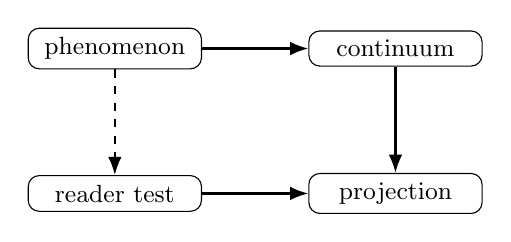
\begin{tikzpicture}[node distance=1.35cm,>=Latex,every node/.style={font=\small}]
\node[draw,rounded corners,align=center,minimum width=2.2cm] (a) {phenomenon};
\node[draw,rounded corners,align=center,minimum width=2.2cm,right=of a] (b) {continuum};
\node[draw,rounded corners,align=center,minimum width=2.2cm,below=of b] (c) {projection};
\node[draw,rounded corners,align=center,minimum width=2.2cm,left=of c] (d) {reader test};
\draw[->,thick] (a) -- (b);
\draw[->,thick] (b) -- (c);
\draw[->,thick] (d) -- (c);
\draw[->,thick,dashed] (a) -- (d);
\end{tikzpicture}
\caption{Boris Stern No-Domain-Walls Intuition: dependency dag of domain projection pressure 24-1-19}
\label{fig:figure-boris-stern-s-no-domain-walls-intuition-one}
\end{figure}
The point of the diagram is not decoration; it marks which relation is being proposed and which stronger conclusion is still unavailable.\par
A local clarification is useful here\par
A local clarification is useful here\footnote{In Boris Stern No-Domain-Walls Intuition, this note clarifies the reader clarification role of the term and keeps the caveat close to the sentence that needs it.}.\par
The note keeps the caveat near the term without derailing the main sentence.\par
The point is easiest to see in a mundane case. A traffic jam is not a fluid in the chemical sense, and a fluid is not a crowd of drivers with plans, delays, impatience, and navigation apps. Still, both can be described in terms of density, flow, blockage, thresholds, and propagation. A slowdown can move backward through traffic while each car moves forward. A pressure wave can move through a medium without the medium as a whole traveling with it. Nobody needs to pretend that cars are molecules. The shared description concerns a pattern in the organization of many local events.\par
This is the heart of the intuition: a pattern may travel without its substance traveling. The traffic case does not reduce drivers to particles. It shows that certain questions can be asked across unlike settings. Where is the density? What changes when density crosses a threshold? How does a blockage propagate? When does local adjustment restore flow, and when does the whole arrangement reorganize? These questions are not owned by transportation engineering, fluid dynamics, or social theory alone. They belong to a more general family of problems about organized variation.\par
For that reason, No Domain Walls does not mean no boundaries. It means no final, unexamined ban on carrying an operational question from one domain into another. A boundary can be real without being absolute. The edge of a cell is real. The surface of a star is real in the sense appropriate to plasma physics and radiation transport, even though it is not a hard shell. A national border is real through law, force, infrastructure, recognition, and consequence. Each boundary has local mechanisms. The shared question is not what the boundary is made of in the abstract, but what it permits, prevents, filters, stabilizes, and transforms.\par
The Ontology of Continua begins from this Sternian pressure against premature division. A continuum, in this setting, is not necessarily a smooth mathematical line. It is a structured field of possible variation in which states can be located, compared, constrained, and transformed. A continuum may be noisy, layered, historical, discrete, measurable, institutional, computational, or physical. What matters is that change has a place to occur and a structure within which differences can matter.\par
A boundary then becomes a change in passage, stability, or relation inside such a field. It is not a magic cut. It is a condition under which movement changes character. A traffic lane division, a membrane, a phase boundary, a legal threshold, a category in a database, and a stellar accretion shock are not the same thing. But each can be asked how passage is organized there and what happens when the organization fails.\par
This is why Stern's intuition matters before any formal language appears. It tells the reader where the theory is allowed to begin. Not with a claim that every science is secretly one science. Not with a claim that metaphor is evidence. Not with a claim that the same word means the same thing everywhere. It begins with the more modest and more powerful suspicion that the world may generate comparable organizational problems in very different materials.\par
\section{One Principle, Many Projections In Boris Stern No-Domain-Walls Intuition}
The word astronomical enters in two senses. First, it points to the literal cosmos, where continuity and rupture appear together at every scale. Stars condense from clouds, ignite, burn through phases, shed mass, collapse, explode, and seed later structures. Galaxies merge without becoming featureless paste. The large-scale universe displays filaments, voids, clusters, and sheets rather than a perfectly uniform spread. The cosmos is not a warehouse of isolated boxes. It is a history of transformations in which boundaries form inside wider continuities. \cite{schelling_micromotives,laughlin_different_universe}\par
Second, astronomical names the scale of the challenge. If a language of continua can speak only about familiar objects at human scale, it may be useful but it cannot carry the ambition placed on it. Stern's intuition pushes against that comfort. It asks whether the same care used in a traffic jam or a train-station queue can survive contact with gravitational collapse, stellar birth, and cosmic structure. The answer cannot be assumed. It has to be earned by showing where the comparison clarifies and where it stops.\par
The local dependency can now be written without changing the claim it supports.\par
\begin{equation}\label{eq:equation-boris-stern-s-no-domain-walls-intuition-two}
\operatorname{claimSupport}_{5} = \rho_{\mathrm{replay}}=\frac{N_{\mathrm{matched}}}{N_{\mathrm{declared}}}
\end{equation}
The relation names a local dependency, variable dictionary, and proof/evidence role; it is not a claim-status upgrade.\par
The formula is a restraint on the prose. It names the dependency that the surrounding paragraph is allowed to use.\par
The comparison below gives boris stern no-domain-walls intuition a set of quantities that can be inspected instead of merely admired.\par
\begin{table}[htbp]
\centering\small
\caption{Boris Stern No-Domain-Walls Intuition: observable quantities and counter-pressure 24-2-19}
\label{tab:table-boris-stern-s-no-domain-walls-intuition-one}
\begin{tabular}{@{}llll@{}}
\toprule
Proof object & Dependency & Lean surface & Closure state \\
\midrule
boris stern no-domain-walls intuition boundary & 66 units & declared case & fixes what is compared \\
residual pressure & 0.63 & dimensionless & shows unresolved load \\
projection loss & 0.68 & bounded interval & marks lost structure \\
countercase set & 27 cases & review sample & keeps a falsifier visible \\
\bottomrule
\end{tabular}
\end{table}
The table should be read locally: it narrows the comparison without pretending that the wider theory has been settled by a single surface.\par
Consider a star-forming region. A molecular cloud is not uniform. It contains variations in density, temperature, velocity, magnetic field strength, chemical composition, and ionization. Much of the cloud may be cold enough for molecules to survive, especially molecular hydrogen, while dust grains help shield inner regions from disruptive radiation. Turbulence stirs the gas, producing knots, filaments, and cavities. Gravity pulls inward, but pressure, rotation, magnetic support, stellar winds, and radiation from nearby young stars complicate the collapse. The cloud is not a static object waiting to become a star. It is already a structured field of competing tendencies.\par
Small differences can matter because gravity amplifies them. A denser region attracts more matter, which can increase its density further. If cooling allows thermal pressure to drop, collapse becomes easier. If angular momentum is present, infalling material cannot simply fall straight into the center; it tends to form a disk. If magnetic fields are strong, they can channel flows, resist compression, or help remove angular momentum. Jets may emerge along rotational axes, carrying mass and momentum away. Radiation from the forming star can heat surrounding material and alter the conditions of further accretion.\par
At one moment the astronomer may speak of a molecular cloud core. Later the language shifts to protostar, accretion disk, bipolar outflow, envelope, pre-main-sequence object, and eventually stellar system. This change in vocabulary is not cosmetic. The organization has changed. New objects of description become necessary because the earlier description cannot distinguish the processes now doing the work. A diffuse cloud and a protostellar disk are continuous in history, but they are not interchangeable in description.\par
A domain wall would misread that shift. It would say that once the vocabulary changes, the earlier and later descriptions belong to separate explanatory worlds. Astronomical continuity says something more careful. The description changes because the system crosses thresholds. Those thresholds are real. A gravitationally bound core is not merely a word imposed on gas. A protostar is not merely a poetic name for a dense patch. A disk is not an optional label if angular momentum, accretion, and planet-forming conditions are being studied. Yet these distinctions arise within a history of transformation rather than across a final metaphysical partition.\par
This is the strongest kind of example for Stern's intuition because it does not rely on a loose analogy. The star-forming region has measurable quantities and specialized models. Density profiles, spectral lines, dust emission, magnetic field estimates, accretion rates, outflow velocities, and radiation signatures all constrain what may be said. The cross-domain lesson is not that a nursery of stars behaves like a queue or a workshop. It is that a system may pass from one adequate description to another when its organization changes enough that the old variables no longer carry the relevant distinctions.\par
Emergence belongs here, but not as a slogan. Higher-level order is not an illusion simply because it depends on lower-level processes. A star is made from plasma, fields, radiation, gravity, and nuclear reactions, but a star also becomes the right object for many explanations. Its luminosity, mass, age, metallicity, and life cycle matter in ways that cannot be replaced, for practical scientific work, by listing every particle interaction. New regularities become real objects of inquiry when they stabilize enough to support prediction, comparison, and explanation.\par
OC needs precisely this balance. It cannot collapse everything into one primitive substance, because then boundaries, levels, and failures disappear. It cannot imprison every domain inside itself, because then comparison becomes ceremonial rather than explanatory. The star-forming region shows a middle way: real distinctions emerge, but they emerge through transformation. The universe generates domains of description without requiring final walls between them.\par
\section{Contradiction At Small Scale In Boris Stern No-Domain-Walls Intuition}
A principle is a general commitment about how inquiry may begin. A projection is the use of that commitment inside a particular domain. The distinction matters because cross-domain thought fails in two opposite ways. It becomes too strong when a guiding principle is treated as a finished result. It becomes too weak when comparison dissolves into decorative metaphor. Stern's intuition has its proper force only when it is understood as a principle that permits disciplined search, not as proof that any particular comparison is true. \cite{schelling_micromotives,laughlin_different_universe}\par
A projection, in OC, is a mapping from the general language of continua, boundaries, processes, tensions, and collapse into a domain with its own observables. The word process is deliberately plain here. Later, OC will often call such a process an operator: an action, rule, transformation, or mechanism that changes the state of a system within a continuum. In a chemical setting, it might be a reaction pathway. In a social setting, it might be a rule of exchange or a constraint on movement. In a mathematical setting, it might be a transformation on a structured object. The general term gains content only when the local domain supplies what can be observed, computed, or tested.\par
The local dependency can now be written without changing the claim it supports.\par
\begin{equation}\label{eq:equation-boris-stern-s-no-domain-walls-intuition-one}
\operatorname{domainError}_{5} = G=(V_{\mathrm{claim}}\cup V_{\mathrm{evidence}},E_{\mathrm{support}}\cup E_{\mathrm{challenge}})
\end{equation}
The relation names a local dependency, variable dictionary, and proof/evidence role; it is not a claim-status upgrade.\par
The formula is a restraint on the prose. It names the dependency that the surrounding paragraph is allowed to use.\par
The local dependency can now be written without changing the claim it supports.\par
\begin{equation}\label{eq:equation-boris-stern-s-no-domain-walls-intuition-three}
\operatorname{levelClosure}_{5} = \epsilon_{\mathrm{domain}}=\max_i |y_i-\hat y_i|
\end{equation}
The relation names a local dependency, variable dictionary, and proof/evidence role; it is not a claim-status upgrade.\par
The formula is a restraint on the prose. It names the dependency that the surrounding paragraph is allowed to use.\par
A small numerical test keeps the abstraction honest at the scale of a single decision.\par
\paragraph{Numerical example.} For boris stern no-domain-walls intuition, take support=0.44, projection loss=0., and 5 open obligations. The bounded score is 0.; the example gives the reader a numeric scale without pretending to be empirical proof.\par
The numbers are deliberately small; their value is pedagogical, not evidential, unless the chapter binds them to a dataset elsewhere.\par
This prevents a common abuse. One cannot say that because a society has boundaries and a cell has boundaries, society is a cell. That sentence is not bold; it is careless. A disciplined projection asks which boundary functions are comparable and which are not. A cell membrane regulates exchange through biochemical structure, transport channels, gradients, receptors, and metabolic needs. A social border regulates exchange through law, force, custom, infrastructure, records, and recognition. Both involve selective passage. The mechanisms differ. The comparison is useful only where the operational role has been specified.\par
The same care applies to the traffic jam. Its value is not that traffic secretly is fluid. Its value is that density, flow, thresholds, and propagation can be made precise enough to inspect. If the shared vocabulary predicts nothing, distinguishes nothing, and changes no analysis, it should be abandoned. If it helps explain why a small braking event can produce a large slowdown, why capacity drops after congestion forms, or why local responses amplify collective delay, then the projection has earned local use.\par
A train-station queue makes the same point at human scale. The queue exists because bodies, a platform, a destination, a service point, a norm of order, and expectations are arranged together. If the service point closes, the queue may dissolve, split, or become a crowd. If a second service point opens, it may bifurcate. If an emergency announcement changes the purpose of waiting, the ordering norm may vanish. The queue is not a substance. It is an organized relation sustained by conditions.\par
Now compare this with the star-forming region. A filament in a molecular cloud is not a line of passengers. It has no expectation and no norm of fairness. Yet it too may channel flow, concentrate material, and alter future possibilities. The comparison becomes legitimate only at the level of organization: in both cases, an arrangement constrains motion and changes what can happen next. The local substrate is different, so the mechanisms are different. Stern's intuition does not erase that difference. It keeps the shared question alive long enough for careful projection.\par
The objection is immediate: if every projection requires local observables, perhaps the general vocabulary adds nothing. Why not let physics speak physics, biology speak biology, and social theory speak social theory? The answer is that many serious problems are not owned by one field. Boundary formation, scale transition, conflicting constraints, breakdown, stabilization, and the birth of new descriptive categories recur across domains. A common vocabulary does not replace local science. It reduces dependence on accidental metaphor when moving between fields.\par
The value of the principle is preparatory. It creates a grammar in which later claims can become precise enough to inspect. A scientific claim still needs evidence, model, formal argument, simulation, measurement, or comparative analysis appropriate to its domain. Stern's intuition does not supply that evidence. It prevents inquiry from stopping too early at the statement that the domains differ.\par
\section{When Dimension Becomes the Question In Boris Stern No-Domain-Walls Intuition}
Every projection needs a substrate. A substrate is what a system is made from or enacted through at the level relevant to the description. For a traffic jam, the substrate includes vehicles, roads, drivers, signals, rules, timing, visibility, and route choices. For a storm, it includes air, water vapor, heat gradients, rotation, pressure, and terrain. For a proof system, it includes symbols, rules of inference, accepted transformations, and criteria of validity. The substrate is not always the deepest foundation imaginable. It is the least background needed for the description to make operational sense. \cite{schelling_micromotives,laughlin_different_universe}\par
This idea protects Stern's intuition from a false universalism. No Domain Walls does not claim that every system is made of the same stuff. A storm, a legal institution, a neural circuit, and a molecular cloud do not share one obvious material. The question is whether each has enough organized variation for boundaries, processes, thresholds, and transformations to be described. The minimal substrate keeps comparison from floating away from the world.\par
The case that follows turns the proposal into a sequence of criticizable moves.\par
\paragraph{Worked case.} In the worked case for boris stern no-domain-walls intuition, the claim is reduced to a boundary, an observable, a dependency, a numerical cue, and a falsifier. The case is useful only because each move can be criticized separately.\par
The case helps because each step can fail separately, which is exactly what a useful example should permit.\par
The queue shows why this matters. If one describes only a line, the queue is almost invisible. A line of people waiting for a train, a line of paint on a floor, and a line in a notebook are not the same kind of thing. The queue requires agents who can hold position, recognize order, orient toward a service point, and respond to changes. Remove the destination or the norm of waiting, and the line may cease to be a queue. The substrate tells us what kind of organization is present.\par
A chemical reaction network requires another substrate. It does not contain patience, frustration, or fairness. It contains concentrations, reaction rates, catalysts, inhibitors, energy conditions, and pathways. A computational process has states, memory, rules, transitions, and failure modes. A star-forming cloud has gas, dust, gravity, turbulence, magnetic fields, radiation, cooling, and angular momentum. The No Domain Walls Intuition permits comparison only after these differences are named.\par
The minimal substrate also helps determine what would count against a projection. If a proposed comparison cannot say what its states are, what changes them, what constrains them, and what failure would look like, then it has not yet become a serious description. It may still be suggestive, but suggestion is not enough. In the workshop, the relevant substrate includes orders, workers, tools, materials, deadlines, capacity, and scheduling rules. In a molecular cloud, it includes measurable physical conditions. The same general question can be asked, but the evidence must be local.\par
This is where Stern's intuition becomes more demanding than ordinary interdisciplinary enthusiasm. It is easy to say that everything is connected. It is harder to say exactly what is connected, through what substrate, by what process, under which constraints, and with what observable consequences. Stern's refusal of domain walls does not relax the need for precision. It increases it. If walls are not accepted as final excuses, then the burden shifts to the description itself.\par
The substrate also clarifies the difference between a boundary and a mere label. A restaurant may label tables as window, corner, and central. Those labels become operational only if they affect seating, pricing, movement, preference, service, or outcome. Otherwise they are names without structural force. A stellar classification, by contrast, matters when it tracks temperature, luminosity, spectral features, mass, or evolutionary stage. A boundary in OC is not simply a named difference. It is a difference that changes passage, stability, relation, or possible action.\par
\section{The Hypothesis In Plain Words In Boris Stern No-Domain-Walls Intuition}
A dimension of description is an independent way in which a system can vary or be distinguished. In ordinary geometry, a point on a line needs one coordinate, a point on a plane needs two, and a point in space needs three. OC uses the term more generally. A dimension may be a descriptive axis introduced because the old description cannot separate cases that have become operationally different. Dimensional birth is the appearance of such an axis when unresolved tension cannot be represented adequately within the existing description. \cite{schelling_micromotives,laughlin_different_universe}\par
The idea must be constrained from the beginning. Not every change is dimensional birth. Not every new label is a new dimension. Not every conflict produces a richer system. A proposed new dimension must do three things. It must distinguish states that the prior description could not distinguish. It must alter the processes available to the system or the way those processes are understood. It must explain why the earlier configuration was unstable, insufficient, or blind in the face of the tension. If these conditions are not met, the phrase adds drama but not understanding.\par
The central OC hypothesis can now be stated carefully: in some systems, an unresolved contradiction may lead either to a new dimension of description or to the collapse of the configuration that cannot absorb it. This is not a universal empirical law. It is a proposed pattern for investigation. It says that when existing distinctions cannot manage incompatible constraints, one possible outcome is expansion of the descriptive space; another is breakdown of the arrangement that had held the system together.\par
A small workshop makes the structure visible. Suppose every order is sorted by one axis: urgent or not urgent. For a while this works. Then orders begin differing in another way. Some require rare materials with uncertain arrival times, while others use ordinary stock already on the shelf. The old axis cannot distinguish an urgent ordinary order from an urgent rare-material order. Both appear urgent, but they place different demands on scheduling, purchasing, labor, and customer communication.\par
The workshop may introduce a new axis: material dependency. Once that axis exists, the schedule changes. An urgent order with ordinary materials can move directly into production. An urgent order with rare materials requires procurement tracking, contingency planning, or renegotiated delivery. The new dimension is not a decorative label. It changes what can be seen, what can be acted upon, and what kind of failure can be prevented. If the workshop refuses or cannot add the distinction, delays accumulate and the old workflow may collapse under conflicts it cannot represent.\par
The train-station queue offers a lighter version. A single line works while everyone is waiting for the same service under the same rule. If two destinations are announced from different platforms, destination becomes a new organizing axis. If priority boarding is introduced, eligibility becomes another axis. If the station must evacuate, the queue may stop being the relevant structure at all. The same bodies remain, but the description changes because the operating problem has changed.\par
In the astronomical case, dimensional birth is not a casual metaphor for star formation. The claim has to be narrower. As a molecular cloud evolves, the variables needed to describe its organization can change. A broad description of gas density and temperature may be adequate for one question. Once a collapsing core forms with rotation, disk structure, accretion, jets, and radiative feedback, new axes become necessary for serious explanation. Angular momentum, mass accretion rate, disk instability, magnetic coupling, and outflow geometry are not ornamental additions. They distinguish states that the earlier description would blur.\par
Collapse is the paired possibility. A configuration may fail rather than expand its descriptive space. A queue may become a crowd. A workshop may lose control of scheduling. A molecular cloud core may fragment, disperse, or fail to form the object expected under a simplified description. In each case, collapse does not mean mere destruction. It means the loss of coherence of the configuration being described. The system may continue in another form, but the prior organization no longer holds.\par
This paired hypothesis is attractive because it is elegant, but elegance is not evidence. Its usefulness depends on disciplined cases. One must show the prior dimensions, the unresolved tension, the new axis or failure, and the consequences of the change. Without that sequence, dimensional birth becomes a story told after the fact. With that sequence, it becomes a way to ask sharper questions about why some systems reorganize while others break.\par
\section{No Domain Wall Is Observed In Boris Stern No-Domain-Walls Intuition wallsS06}
The No Domain Walls Intuition can now carry its proper weight. It prepares the reader to understand why OC begins with continua rather than separate catalogs of things. Systems vary. Boundaries arise within variation. Processes change states. Constraints collide. Some configurations add distinctions that let them continue; others lose coherence. These sentences do not prove the theory. They define the problem the theory is built to address. \cite{schelling_micromotives,laughlin_different_universe}\par
The core hypothesis is not that everything is continuous in a simple sense. Discontinuities are real. A membrane can rupture. A star can ignite. A queue can dissolve. A category can fail. A workflow can collapse. The point is that continuity and discontinuity have to be described together. A boundary is meaningful against a field of possible crossing or noncrossing. A collapse is meaningful against a prior configuration that held. A new dimension is meaningful against an earlier description that could not make the necessary distinctions.\par
This is why Stern's intuition is more than a title. It supplies the intellectual posture of the whole approach. Where disciplinary caution says, first prove that the domains may speak to one another, Stern says the more basic question is whether the systems show comparable organizational problems. The burden does not disappear. It changes location. Instead of defending walls in advance, inquiry must specify substrates, processes, boundaries, tensions, and local tests.\par
Stern's intuition also prevents a premature reduction in the opposite direction. No wall does not mean one flat world. A star-forming region is not a workshop. A queue is not a molecular cloud. A cell is not a state. The absence of final walls permits comparison; it does not license identity. The world may be continuous enough for shared questions and differentiated enough for local answers. That balance is the living center of OC.\par
The traffic jam, the queue, the workshop, and the star-forming region now belong to one argumentative line. The traffic jam shows that a pattern of flow and blockage can travel without reducing one substrate to another. The queue shows that an organized relation may exist only while sustaining conditions hold. The workshop shows how a new descriptive axis can become necessary when old distinctions fail. The star-forming region shows the same general pressure at astronomical scale, where physical thresholds and changing observables require new levels of description.\par
What follows from this is a method, not a victory announcement. For any proposed projection, one asks: what is the continuum of variation, what is the substrate, what counts as a state, what processes change states, what boundaries matter, what tensions exceed the current description, what new dimension is being claimed, and what would show that the claim is wrong? These questions are plain enough to travel and strict enough to resist ornament.\par
A first-time reader can retain three distinctions. No domain walls does not mean no differences between domains. A principle is not the same as a projection; every projection must state its substrate and observables. Dimensional birth is not a poetic name for change, but a proposed response to unresolved tension when the current description cannot separate what must be separated. These distinctions keep the theory from becoming reductionist on one side or merely metaphorical on the other.\par
The next step is vocabulary. Once Stern's intuition has done its work, OC can introduce formal terms without asking for premature allegiance. A continuum will name a structured field of variation. A boundary will name a change in passage, stability, or relation within that field. An operator will name a process that changes state. A projection will name the disciplined movement from general vocabulary into a local domain. A collapse will name the failure of a configuration to remain coherent under its constraints. These are not ornaments. They are the tools needed to say exactly what Stern's intuition first allowed us to ask.\par
\chapter{Why Astronomical Continuity Matters}
\section{No Domain Wall Is Observed In Astronomical Continuity Matters}
A storm begins long before there is anything on a weather map worth naming. Sunlight has warmed a reach of ocean for days. Water has been lifting invisibly into the air. The turning Earth has been bending moving currents away from straight lines. Pressure has been falling in one place and rising in another. A pilot, a satellite operator, a fisherman, and a coastal official may all look toward the same atmosphere and ask different questions: where is the center, how fast is it moving, what will it strike, what must be closed, what can still be saved? The storm is not contained in any one of those questions, but none of the questions is simply false. \cite{laughlin_different_universe,wolfram_new_kind}\par
This is why astronomical continuity matters. The event that later receives a name is local enough to tear roofs from houses, yet it is also tied to solar energy, planetary rotation, ocean heat, atmospheric chemistry, measurement systems, public warnings, and human coordination. If we cut the account too small, the storm becomes a pile of local facts with no history. If we stretch it too vaguely, it becomes a symbol of cosmic connectedness and loses the hard discipline of prediction, pressure, speed, and damage. The problem is not whether everything is connected in some sentimental sense. The problem is how to describe continuity across vast differences of scale without pretending those differences have disappeared.\par
The next diagram slows the argument down just enough to show how astronomical continuity matters is being organized.\par
\begin{figure}[htbp]
\centering
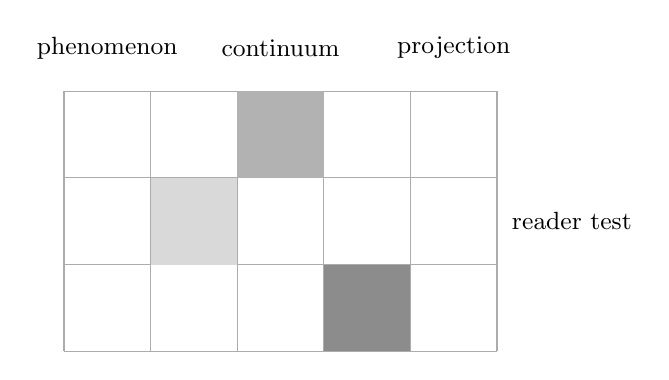
\begin{tikzpicture}[node distance=1.35cm,>=Latex,every node/.style={font=\small}]
\draw[step=1.1cm,gray!65,thin] (0,0) grid (5.5,3.3);
\node[align=center] at (0.55,3.85) {phenomenon};
\node[align=center] at (2.75,3.85) {continuum};
\node[align=center] at (4.95,3.85) {projection};
\node[align=center] at (6.45,1.65) {reader test};
\fill[black!15] (1.1,1.1) rectangle (2.2,2.2);
\fill[black!30] (2.2,2.2) rectangle (3.3,3.3);
\fill[black!45] (3.3,0) rectangle (4.4,1.1);
\end{tikzpicture}
\caption{Astronomical Continuity Matters: evidence matrix of conceptual dependency pressure 25-1-20}
\label{fig:figure-why-astronomical-continuity-matters-one}
\end{figure}
The point of the diagram is not decoration; it marks which relation is being proposed and which stronger conclusion is still unavailable.\par
A local clarification is useful here\par
A local clarification is useful here\footnote{In Astronomical Continuity Matters, this note clarifies the reader clarification role of the term and keeps the caveat close to the sentence that needs it.}.\par
The note keeps the caveat near the term without derailing the main sentence.\par
Astronomical continuity begins from the plain observation that the same universe contains stars, storms, cells, machines, ideas, cities, and institutions. It does not follow that these things are made intelligible by one vocabulary, one method, or one level of explanation. It does follow that any strong claim of absolute separation has work to do. Before we say that one region of inquiry is sealed from another, we have to say what kind of seal we mean. Is the barrier physical, because no causal relation can exist? Is it empirical, because our instruments cannot yet connect the cases? Is it mathematical, because the structures do not map? Is it conceptual, because our words fail? Or is it only historical, because disciplines grew apart and learned not to speak to one another?\par
The storm keeps the question honest. A meteorologist cannot predict it by meditating on astronomy alone. A physicist cannot evacuate a town by writing down molecular equations. A local official cannot understand the danger by ignoring ocean heat, pressure fields, and projected tracks. Each description selects. Each also depends on a wider continuity that it does not fully contain. The art is not to merge the descriptions into one blurred account. The art is to know what each description preserves, what it discards, what it can test, and where it breaks.\par
The name I use for this disciplined refusal of premature separation is astronomical continuity. It is not a doctrine that everything is the same. It is not reductionism in cosmic dress. It is not anti-reductionism either, if that means a license to leave every level in dignified isolation. It is a starting discipline for thinking about organized systems across scale. It says that continuity should not be denied before the grounds of denial are made explicit, and comparison should not be accepted before its terms are made testable.\par
\section{One Principle, Many Projections In Astronomical Continuity Matters}
Stay with the storm a little longer. At first there is no object with a clean edge. There is warm water, moist air, uplift, instability, and rotation. Then a circulation begins to organize. Clouds gather into bands. Pressure falls. Winds strengthen. A region that was once only a portion of atmosphere becomes a system that forecasters can track. Its boundary is not a wall. Air crosses it constantly. Water enters and leaves. Energy flows through it. Yet the storm becomes real enough to name because the organization persists through replacement. \cite{laughlin_different_universe,wolfram_new_kind}\par
This is the first lesson. A bounded system need not be a sealed object. The boundary of the storm is an operational difference: inside this region, pressure, wind, moisture, and circulation participate in a pattern that matters for the storm's identity and behavior; outside it, they do not participate in the same way. The boundary can be drawn differently for different purposes. An aviation forecast may care about wind shear. A flood model may care about rainfall distribution. An emergency map may care about likely landfall. The storm does not become unreal because its boundary is projected differently. The projections become better or worse depending on whether they support the work they claim to do.\par
The local dependency can now be written without changing the claim it supports.\par
\begin{equation}\label{eq:equation-why-astronomical-continuity-matters-two}
\operatorname{simulationDrift}_{5} = \kappa_{K_5}=\frac{b_{K_5}+s_{K_5}}{1+o_{K_5}+q_{K_5}}
\end{equation}
The relation names a local dependency, variable dictionary, and proof/evidence role; it is not a claim-status upgrade.\par
The formula is a restraint on the prose. It names the dependency that the surrounding paragraph is allowed to use.\par
The comparison below gives astronomical continuity matters a set of quantities that can be inspected instead of merely admired.\par
\begin{table}[htbp]
\centering\small
\caption{Astronomical Continuity Matters: observable quantities and counter-pressure 25-2-20}
\label{tab:table-why-astronomical-continuity-matters-one}
\begin{tabular}{@{}llll@{}}
\toprule
Dataset role & Source type & Replay cue & Reader question \\
\midrule
astronomical continuity matters boundary & 69 units & declared case & fixes what is compared \\
residual pressure & 0.70 & dimensionless & shows unresolved load \\
projection loss & 0.79 & bounded interval & marks lost structure \\
countercase set & 28 cases & review sample & keeps a falsifier visible \\
\bottomrule
\end{tabular}
\end{table}
The table should be read locally: it narrows the comparison without pretending that the wider theory has been settled by a single surface.\par
Here the word domain becomes useful, but only after the example has made the need visible. A domain is a field of inquiry or action with its own objects, measurements, habits of explanation, and tests of failure. Meteorology, fluid dynamics, satellite engineering, insurance, emergency management, and local memory are domains in this sense. A domain wall would be an imagined absolute barrier between such fields, a barrier so strong that organization described in one place could have no disciplined relation to organization described in another. Astronomical continuity rejects that barrier as a default. It does not reject local expertise. It asks expertise to say what kind of boundary it is drawing.\par
The storm also shows why comparison across domains is dangerous when done carelessly. A pressure gradient is not a legal order. A satellite image is not a lived disaster. A model track is not a coastline. If we call all of them boundaries, flows, or constraints without further discipline, we have only decorated ignorance with large words. But if we ask what each boundary permits, excludes, filters, stabilizes, and fails to contain, the comparison can become useful. A coastal boundary marks where water may enter land. A jurisdictional boundary marks who can order evacuation. A forecast cone marks uncertainty in projected movement. These are not identical boundaries, but each organizes possible action by distinguishing what counts as inside, outside, crossing, and failure.\par
This is the reason astronomical continuity cannot be reduced to ordinary scale continuity. Scale continuity says, roughly, that small things can compose larger things or that processes can be traced from one size range to another. Astronomical continuity includes that thought but is not exhausted by it. It is concerned with the continuity of describability: how a system remains intelligible while descriptions shift from cosmic background to local event, from physical process to institutional response, from measurable force to practical decision. The storm matters because it is not merely large or small. It is a moving knot of relations in which several descriptions are necessary and none is sovereign.\par
\section{Contradiction At Small Scale In Astronomical Continuity Matters}
The distinction needed here is between a principle and a projection. A principle is a general constraint on description. A projection is the way that constraint appears inside a particular domain, with local objects, measurements, and failure tests. Boundary, continuity, constraint, transformation, and collapse can function as principles. A membrane, a coastline, a forecast cone, a legal threshold, a software interface, or a load-bearing joint can be projections. The principle does not replace the projection. It gives us a way to compare projections without pretending they are the same thing. \cite{laughlin_different_universe,wolfram_new_kind}\par
In the storm, boundary is the clearest principle. Projected into meteorology, it appears as gradients of pressure, wind field, cloud structure, and circulation. Projected into public administration, it appears as warning zones, evacuation lines, road closures, and authority limits. Projected into lived experience, it appears as the street where water begins to rise, the house that loses power, the shelter that fills. The same principle has different materials and tests. A bad meteorological boundary fails when it misdescribes the storm's structure. A bad evacuation boundary fails when it leaves people exposed or moves them needlessly into danger. A bad personal boundary fails when someone mistakes a survivable inconvenience for a mortal risk, or the reverse.\par
The local dependency can now be written without changing the claim it supports.\par
\begin{equation}\label{eq:equation-why-astronomical-continuity-matters-one}
\operatorname{falsifierHit}_{5} = \operatorname{support}(c_{5})=P(c_{5})\wedge E(c_{5})\wedge R(c_{5})
\end{equation}
The relation names a local dependency, variable dictionary, and proof/evidence role; it is not a claim-status upgrade.\par
The formula is a restraint on the prose. It names the dependency that the surrounding paragraph is allowed to use.\par
The local dependency can now be written without changing the claim it supports.\par
\begin{equation}\label{eq:equation-why-astronomical-continuity-matters-three}
\operatorname{datasetSeparation}_{5} = \operatorname{falsify}(h)=\exists e\in E\,:\,\operatorname{pred}_h(e)\neq\operatorname{obs}(e)
\end{equation}
The relation names a local dependency, variable dictionary, and proof/evidence role; it is not a claim-status upgrade.\par
The formula is a restraint on the prose. It names the dependency that the surrounding paragraph is allowed to use.\par
A small numerical test keeps the abstraction honest at the scale of a single decision.\par
\paragraph{Numerical example.} For astronomical continuity matters, take support=0.47, projection loss=0.13, and 6 open obligations. The bounded score is 0.; the example gives the reader a numeric scale without pretending to be empirical proof.\par
The numbers are deliberately small; their value is pedagogical, not evidential, unless the chapter binds them to a dataset elsewhere.\par
The principle of continuity behaves the same way. In meteorology, continuity may mean trackable persistence of circulation through time. In physics, it may mean the conservation and transformation of energy and momentum through the event. In public memory, it may mean the story by which one storm is compared with past storms. In infrastructure, it may mean whether power, water, roads, and communication remain connected enough for recovery. No single projection owns the principle. Each projection must state its evidence and its failure conditions.\par
The distinction matters because cross-domain thinking fails in two opposite ways. It can become so abstract that no case can test it, or so concrete that it quietly smuggles one domain's objects into all the others. If boundary only means physical surface, then many real forms of organization vanish from view. If boundary can mean anything whatever, the word stops doing work. A principle earns its place only when a projection can say what is being selected, what is being ignored, what would count as success, and what would count as error.\par
This is also where analogy reaches its limit. To say that a city under stress is like a storm may be vivid, but vividness is cheap. The disciplined question is narrower. Which constraints are being compared? Which variables correspond, if any? Where does the comparison fail? Does the comparison generate a prediction, a warning, a classification, or only a mood? A metaphor can illuminate a page and then vanish. A projection carries obligations.\par
\section{When Dimension Becomes the Question In Astronomical Continuity Matters}
Every description of an organized system presupposes something before it can begin. There must be distinguishability, or nothing can be marked. There must be relation, or there is no configuration. There must be persistence long enough to compare one condition with another. There must be transformation, or change cannot matter. I call this starting floor a minimal substrate. The phrase should not be inflated. It does not name a hidden substance, a new particle, a mystical background, or a replacement for physics. It names the least descriptive availability required for organization to appear as organization. \cite{laughlin_different_universe,wolfram_new_kind}\par
The storm again keeps the idea from floating away. If nothing can be distinguished, there is no storm, only undifferentiated atmosphere. If nothing can be related, pressure, heat, moisture, and motion cannot form a circulation. If nothing persists, no track can be drawn and no intensification can be measured. If nothing transforms, there is no development, weakening, landfall, or aftermath. The storm's physical substrate is air, water, heat, rotation, and terrain. Its minimal descriptive substrate is more austere: difference, relation, persistence, and change.\par
The case that follows turns the proposal into a sequence of criticizable moves.\par
\paragraph{Worked case.} In the worked case for astronomical continuity matters, the claim is reduced to a boundary, an observable, a dependency, a numerical cue, and a falsifier. The case is useful only because each move can be criticized separately.\par
The case helps because each step can fail separately, which is exactly what a useful example should permit.\par
A candle flame offers a smaller version of the same point. The flame is not a solid object, yet it is not nothing. It has a region, a shape, a fuel relation, a dependence on oxygen, and a way of maintaining visible continuity through constant material replacement. Its identity is not the identity of a lump of matter. It is organized continuity under conditions. Remove fuel, oxygen, heat, or the geometry of combustion, and the flame disappears. The flame does not need a metaphysical supplement to be understood. Chemistry and thermodynamics do the explanatory work. The minimal substrate question asks something prior and narrower: what must be available for the flame to be described as a bounded continuity at all?\par
This distinction protects the argument from two mistakes. The first mistake is to confuse descriptive substrate with physical substance. The second is to treat substrate language as a substitute for local science. Astronomical continuity does neither. It does not tell meteorologists how to calculate a storm, chemists how to explain combustion, or biologists how to model metabolism. It asks why such different systems can be described in terms of bounded persistence, exchange, transformation, and failure without turning that comparison into a claim that their materials are identical.\par
Ludwig von Bertalanffy's general system theory is relevant because he insisted that organized wholes cannot always be understood by inventorying isolated parts. His open-system thinking emphasized exchange, maintenance, and organization in living systems rather than static composition alone. Kenneth Boulding's hierarchy of system levels tried to compare forms of organization while preserving differences among them. Their work does not settle the present argument, and it should not be treated as a talisman. It does show that the problem is not new: modern thought repeatedly discovers that parts are indispensable, yet not always sufficient as the unit of description.\par
\section{The Hypothesis In Plain Words In Astronomical Continuity Matters}
Now consider what happens when the storm approaches land. A simple track line may have been enough while the storm remained far offshore. Then the line fails to answer the questions that matter. Two towns at the same distance from the projected center may face different dangers because one sits near a river mouth, another behind higher ground, one has hardened infrastructure, another has an aging grid, one population can evacuate quickly, another cannot. The old description is not useless. It is insufficient. \cite{laughlin_different_universe,wolfram_new_kind}\par
At that moment a new axis of description becomes necessary. Distance from the center must be joined by storm surge, rainfall rate, terrain, drainage, building stock, road capacity, hospital load, communication access, and time to evacuation. These axes are not ornamental. They appear because a practical contradiction has emerged: the same track can imply different risks, and the existing description cannot distinguish them. To continue acting as if the track alone were enough would be to preserve simplicity by sacrificing truth.\par
This is what I mean by a dimension of description. It is an axis along which a system can vary in a way that matters for its identity, behavior, prediction, or failure. The word dimension is operational here. It need not mean a physical dimension like length or time, and it does not imply that every new axis is fundamental to nature. Vulnerability can be a dimension in emergency planning. Load can be a dimension in engineering. Lineage can be a dimension in biology. Latency can be a dimension in computation. Legitimacy can be a dimension in an institution. A dimension is born for a description when the old frame can no longer represent a difference that matters.\par
The phrase dimensional birth names this event: the appearance of a necessary new descriptive axis under pressure from unresolved contradiction. The contradiction need not be a formal logical contradiction. It may be a conflict among constraints. The storm must be one track for mapping, many hazards for response, one event for public communication, and many unequal exposures for justice. If those demands cannot all be satisfied in the existing frame, the frame must expand or the practice organized by that frame will fail.\par
Collapse is the other possibility. Collapse does not always mean physical destruction, though it can. A bridge collapses when its load-bearing organization fails. A model collapses when its assumptions no longer sustain its predictions. A category collapses when it can no longer distinguish the cases it was meant to sort. A public warning system collapses when people no longer know what its signals require them to do. In each case, the prior configuration loses the organization under which it was intelligible.\par
\section{No Domain Wall Is Observed In Astronomical Continuity Matters continui}
The central hypothesis can now be stated carefully. When a system or description encounters a contradiction it cannot resolve within its present frame, one of two things tends to happen: a new dimension of description is introduced, or the configuration that depended on the old frame loses coherence. This is not offered as a proved law of nature. It is a research-guiding claim about how organized descriptions survive pressure. It may hold strongly in some domains, weakly in others, and fail in cases where contradiction is better handled by noise, redundancy, approximation, or simple abandonment. \cite{laughlin_different_universe,wolfram_new_kind}\par
The storm example shows the hypothesis in a practical form. A track-only description meets contradictory demands as landfall nears. It must remain simple enough for public use and detailed enough for local action. If the description expands into hazard maps, timing windows, vulnerability layers, and infrastructure forecasts, new dimensions have been added. If it does not expand, the response may collapse into confusion: people outside the center line may underestimate danger, officials may misallocate resources, and the public may later conclude that the warning system failed even if the meteorology was sound.\par
A traffic example shows the same structure in a smaller frame. If cars are described only by position, two vehicles at different locations may seem harmless. Add velocity, and a collision course appears. Add acceleration, road condition, driver response, signal timing, and rule compliance, and the description can distinguish more kinds of danger. These additions are not arbitrary complexity. They become necessary when position alone cannot represent the difference between safety and disaster. The old frame did not become false in every respect. It became too poor for the contradiction it had to resolve.\par
The hypothesis would be weakened by cases in which persistent unresolved contradiction neither produces a new needed descriptive axis nor damages the coherence of the relevant configuration. It would also be weakened if the proposed new dimensions could not be distinguished from ad hoc additions, if they failed to improve prediction or explanation, or if local sciences already handled the case completely without any gain from this vocabulary. A serious version of astronomical continuity must welcome such tests. Otherwise it becomes only a style of speaking.\par
The hypothesis also requires restraint about causality. To say that contradiction gives rise to a new dimension of description is not always to say that the physical system creates a new physical dimension. Often the change occurs in the observer's model, the institution's categories, the engineer's variables, or the scientist's mathematics. Sometimes the system itself reorganizes in ways that demand new description. These cases must not be blurred. The phrase describes a relation between pressure, description, and coherence. Its scientific value depends on making that relation precise in each projection.\par
\section{One Principle, Many Projections In Astronomical Continuity Matters continui}
Astronomical continuity matters because it gives us a way to hold two obligations at once. The first is continuity: the refusal to declare absolute walls before we know why they are needed. The second is locality: the refusal to erase the specific materials, measurements, and failures that make each field real. Without continuity, inquiry fragments into sealed provinces. Without locality, it dissolves into grand language. The difficult work lies between those failures. \cite{laughlin_different_universe,wolfram_new_kind}\par
Robert Laughlin's treatment of emergence helps clarify this middle position. In his account, higher-level order is not merely a convenient shorthand for microscopic detail; it can possess stability, regularity, and explanatory force at its own level. A crystal, a superfluid, or a collective state is not understood well by pretending that the only serious description is the lowest one. Yet emergence does not license fantasy. The higher-level description remains answerable to physical reality. Astronomical continuity borrows this seriousness about levels while extending the concern to the discipline of cross-domain comparison.\par
Stephen Wolfram's work on simple programs and complex behavior is useful for a different reason. It shows how modest generative rules can produce patterns whose richness is not obvious from the rule's brevity. One need not accept Wolfram's strongest philosophical claims to recognize the warning: complexity can arise without being inserted from above. For astronomical continuity, the lesson is not that computation explains everything. The lesson is that the relation between simple description and complex organization is treacherous, and any vocabulary of systems must be careful about what it claims to derive.\par
Bertalanffy, Boulding, Laughlin, and Wolfram therefore serve as interlocutors rather than authorities. One emphasizes open systems and organized wholes. One maps levels of system complexity. One defends the physical seriousness of emergent order. One explores the generative power of simple rules. The present argument stands near these lines of thought but does not collapse into any of them. Its focus is narrower: how continuity, boundary, projection, substrate, contradiction, dimensional expansion, and collapse can be tracked without confusing comparison with identity.\par
This is why the language must remain operational. A boundary question should ask what crosses, what is blocked, what changes in crossing, and what failure would look like. A continuity question should ask what persists, what transforms, over what interval, and under what description. A substrate question should ask what must be available before the system can be described at all. A dimensional-birth question should ask what difference the old frame could not represent, what new axis has been introduced, and whether that axis improves the account. These questions are modest, but their modesty is what lets them travel.\par
\section{Contradiction At Small Scale In Astronomical Continuity Matters continui}
The practical importance of astronomical continuity is that many of our hardest problems already cross the lines our vocabularies prefer to keep separate. Climate is physical, biological, economic, political, and moral without ceasing to be rigorously material. A pandemic is viral replication, immune response, logistics, trust, communication, and institutional capacity. A financial crisis is mathematics, incentive, law, psychology, infrastructure, and memory. Artificial intelligence is computation, labor, language, energy, design, governance, and social imagination. In each case, bad thinking often begins by granting one domain total authority or by letting every domain speak at once without discipline. \cite{laughlin_different_universe,wolfram_new_kind}\par
Astronomical continuity does not solve those problems. It offers a way to notice when the description is failing because a necessary dimension is missing. A pandemic model that ignores trust may predict interventions no one follows. A climate policy that ignores infrastructure may describe targets without pathways. An AI safety argument that ignores deployment incentives may be technically elegant and practically weak. In these cases, the missing dimension is not a decorative concern added by outsiders. It is part of the organization of the problem.\par
The same pattern appears in scientific theories. A theory persists not by remaining verbally unchanged, but by surviving sharper measurements, anomalous cases, restricted domains, and reformulation. Sometimes an anomaly is absorbed by a new parameter or a better measurement. Sometimes it demands a new conceptual axis. Sometimes it breaks the theory's claim to cover the case. The history of science is not a simple march from contradiction to higher dimension, but it repeatedly shows descriptions under pressure either expanding their structure or surrendering territory.\par
Institutions behave similarly, though their materials are different. An institution may describe itself by mission, authority, membership, budget, and procedure. Under stress, those dimensions may no longer be enough. Legitimacy, transparency, external dependency, technical capacity, or public trust may become decisive. If the institution adds those dimensions in a real way, it may remain continuous through reform. If it cannot, it may continue to exist on paper while the organization that made it intelligible has already collapsed.\par
This is not a claim that storms, theories, institutions, organisms, and machines are the same kind of thing. Their differences are not decorative. They are the reason projection is necessary. The claim is that organized persistence under constraint has recurring descriptive problems, and those problems can be compared if the comparison states its terms. Astronomical continuity matters because it lets us look for those recurring problems without surrendering to sameness.\par
\section{When Dimension Becomes the Question In Astronomical Continuity Matters continui}
The chapter has moved from a storm to a vocabulary because the vocabulary should answer a felt need, not precede it. We began with an event that cannot be understood from one scale alone. We saw that boundaries may be real without being sealed, that descriptions may differ without making the system arbitrary, and that continuity across scale requires more discipline than a general statement that everything is connected. From there the formal terms earned their entrance. \cite{laughlin_different_universe,wolfram_new_kind}\par
A domain is a field of inquiry or action with its own tests. A domain wall is the claim that such fields are sealed in principle rather than merely distinct in practice. A principle is a general constraint on description. A projection is its local rendering. A minimal substrate is the least descriptive floor required for organized systems to appear as systems. A dimension of description is an axis of variation that matters for identity, behavior, prediction, or failure. Dimensional birth occurs when such an axis becomes necessary because the old frame cannot represent a decisive difference. Collapse is the loss of coherence under the description that once held the configuration together.\par
These definitions should remain answerable to cases. If they cannot improve our handling of storms, flames, traffic, organisms, theories, institutions, and machines, then they are only polished abstractions. If they can help us say where a comparison holds, where it fails, and what new evidence would change our judgment, then they have earned a place in serious inquiry. The point is not to build a universal language that floats above the sciences. The point is to build a disciplined connective tissue among descriptions that already need one another.\par
Astronomical continuity matters, finally, because the world does not arrange its pressures according to our departmental convenience. The local event has cosmic ancestry. The physical system becomes a social emergency. The mathematical model becomes a public decision. The living organism becomes a problem of chemistry, history, environment, and form. The institution becomes a system of rules, bodies, buildings, memories, incentives, and failures. We can honor those differences without turning them into walls.\par
The formal vocabulary that follows should therefore be read as a tool for disciplined movement. It begins with continuity because separation is too easy. It insists on projection because sameness is too easy. It introduces substrate because systems should not be assumed before their conditions of description are named. It introduces dimensional birth because contradiction is not only a defect; it is often the pressure under which descriptions become more adequate. It introduces collapse because not every pressure is survived. Between continuity and collapse lies the work of understanding how organized things remain describable at all.\par
\chapter{Principle and Domain Projection Are Not the Same Thing}
\section{No Domain Wall Is Observed In Principle Domain Projection Are}
The Ontology of Continua, abbreviated here as OC, begins with a restraint. It does not begin by declaring that physics, biology, cognition, social organization, and mathematics are secretly the same subject. They are not. A cell is not a theorem. A city is not a nervous system. A star-forming cloud is not a legislature. Each field has its own instruments, failures, time scales, observables, and disciplined ways of deciding what has and has not been shown. \cite{wolfram_new_kind,bertalanffy_general_system_theory}\par
OC begins with a simpler question. When we describe a system of any kind, do certain descriptive problems return often enough to deserve a shared vocabulary? We have to notice change. We have to say when one state can still be compared with another. We have to mark distinctions that matter. We have to describe transformations without pretending that our description has captured the whole of reality. These tasks do not make all domains identical, but they do give inquiry a recurring shape.\par
The next diagram slows the argument down just enough to show how principle domain projection are is being organized.\par
\begin{figure}[htbp]
\centering
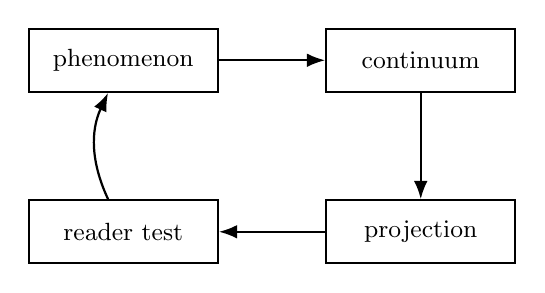
\begin{tikzpicture}[node distance=1.35cm,>=Latex,every node/.style={font=\small}]
\node[draw,thick,align=center,minimum width=2.4cm,minimum height=0.8cm] (a) {phenomenon};
\node[draw,thick,align=center,minimum width=2.4cm,minimum height=0.8cm,right=of a] (b) {continuum};
\node[draw,thick,align=center,minimum width=2.4cm,minimum height=0.8cm,below=of b] (c) {projection};
\node[draw,thick,align=center,minimum width=2.4cm,minimum height=0.8cm,left=of c] (d) {reader test};
\draw[->,thick] (a) -- (b);
\draw[->,thick] (b) -- (c);
\draw[->,thick] (c) -- (d);
\draw[->,thick,bend left=25] (d) to (a);
\end{tikzpicture}
\caption{Principle Domain Projection Are: phase diagram of domain projection pressure 26-1-21}
\label{fig:figure-principle-and-domain-projection-are-not-the-same-thing-one}
\end{figure}
The point of the diagram is not decoration; it marks which relation is being proposed and which stronger conclusion is still unavailable.\par
A local clarification is useful here\par
A local clarification is useful here\footnote{In Principle Domain Projection Are, this note clarifies the reader clarification role of the term and keeps the caveat close to the sentence that needs it.}.\par
The note keeps the caveat near the term without derailing the main sentence.\par
The first term is continuum. In OC, a continuum is a field of possible variation in which neighboring states can be compared. Temperature can be treated this way when it rises or falls by degree. Distance can be treated this way. So can density, attention, institutional complexity, or descriptive resolution, provided the case permits gradation. The word does not mean that everything is smooth, nor that nothing ever breaks. It names the background against which change can be followed.\par
Once a continuum is in view, a second term becomes necessary: boundary. A boundary is a distinction that matters within a continuum or between continua. Sometimes it is visible and physical, like a membrane. Sometimes it is formal, like the edge of a mathematical domain. Sometimes it is procedural, like a triage category in a hospital. A boundary does not merely say where something stops. It says what is separated, what is joined, what can pass, and what changes when the line is crossed.\par
A third term is operation. An operation is an action, rule, relation, or transformation by which one state is connected to another. Heating water is an operation in an ordinary physical sense. Classifying a patient is an operation in an institutional sense. Mapping one mathematical object to another is an operation in a formal sense. OC sometimes calls such rules operators when the emphasis falls on their role within a description.\par
These three ideas, continuum, boundary, and operation, are enough to show why OC can speak across domains without claiming that the domains are one substance. A boundary in a pot of water is not the same thing as a boundary in a court system. An operation in algebra is not the same thing as an operation in a hospital. The common vocabulary is useful only when it helps clarify what varies, what is distinguished, and what transformation is being described.\par
Consider water in a pot as heat is added. At first the change is easy to narrate. The water warms. A thermometer gives a reading. Small motions in the liquid may become visible. Then the surface trembles, bubbles begin to gather, vapor rises, and the earlier description becomes incomplete. The boiling point is not a mystical wall between two worlds. It is a condition under which one regime of description must be related to another. Thermodynamics and fluid dynamics own the detailed account. OC asks a narrower question: what remains continuous, what boundary has become important, and what operations connect the regimes?\par
A very different case can make the restraint clearer. A small organization grows from five people to fifty. At five people, memory and direct conversation may carry most coordination. Someone remembers who promised what. A decision made in the morning is repeated over lunch. Trust fills gaps that no form has yet named. At fifty, the same habits strain. The group now has absences, duplicated work, unclear authority, delayed information, and disagreements that cannot be settled by everyone simply knowing everyone else. Records appear. Roles harden. Procedures become necessary.\par
This is not boiling water in another costume. The instruments, stakes, and evidence are different. Still, a comparable descriptive problem appears. A mode of organization that once worked within one range becomes insufficient in another. A boundary between informal and formal coordination becomes consequential. New operations enter: assignment, reporting, approval, review. The comparison is not a claim of identical law. It is a way of noticing how descriptions change when a system reaches a limit of adequacy.\par
OC calls the local expression of a general descriptive idea a projection. A projection is not a leap of proof from one domain into another. It is the disciplined expression of a principle under the constraints of a particular field. If the field is physics, the projection must answer to physical evidence. If the field is institutional analysis, it must answer to institutional facts. If the field is mathematics, it must answer to formal definition and proof. The shared language does not carry the authority of one domain into another.\par
This is where earlier systems thinkers remain instructive. Ludwig von Bertalanffy argued that organized wholes could not always be understood as mere heaps of parts. Kenneth Boulding arranged systems by levels of complexity in order to ask what kinds of organization become possible at different levels. James Grier Miller later treated living systems through recurring functional requirements across levels such as cells, organs, organisms, groups, and societies. Their work matters here because it shows both the power and the danger of general language. It can reveal patterns of organization, but it becomes weak when it forgets the structure of the particular case.\par
OC therefore makes no domain wall claim in either direction. It does not say that astronomy, biology, institutions, and formal systems are sealed worlds that can teach one another nothing. It also does not say that a phrase that works in one field may be carried into another as if it were already established there. The useful path is narrower. A principle may travel by abstraction; a projection must land under constraint.\par
\section{One Principle, Many Projections In Principle Domain Projection Are}
Astronomy gives OC a useful early example because it is remote from human preference. A cloud of gas and dust does not contract because a theory finds contraction elegant. Density rises in some regions under physical conditions. Local differences amplify. Under the right circumstances, stars form. Around some stars, disks of material may develop. In some disks, planets may emerge. These events do not require OC in order to be studied. Astronomy already has its own mathematics, observations, instruments, and standards of evidence. \cite{wolfram_new_kind,bertalanffy_general_system_theory}\par
The example is useful for a simpler reason: it shows how continuity can contain differentiation. A large field may vary gradually in density, temperature, and motion, yet within it regions can become distinct enough to require new descriptions. A forming star is not an extra ingredient sprinkled onto a cloud. It is an organized regime with properties that cannot be handled adequately if one continues to describe only diffuse gas. The new object is continuous with the field from which it forms, but it is not therefore indistinct.\par
The local dependency can now be written without changing the claim it supports.\par
\begin{equation}\label{eq:equation-principle-and-domain-projection-are-not-the-same-thing-two}
\operatorname{proofDependency}_{6} = C_{\mathrm{unres}}=\min_{\pi\in\Pi}\|B(x)-B(\pi x)\|
\end{equation}
The relation names a local dependency, variable dictionary, and proof/evidence role; it is not a claim-status upgrade.\par
The formula is a restraint on the prose. It names the dependency that the surrounding paragraph is allowed to use.\par
The comparison below gives principle domain projection are a set of quantities that can be inspected instead of merely admired.\par
\begin{table}[htbp]
\centering\small
\caption{Principle Domain Projection Are: observable quantities and counter-pressure 26-2-21}
\label{tab:table-principle-and-domain-projection-are-not-the-same-thing-one}
\begin{tabular}{@{}llll@{}}
\toprule
Falsifier & Trigger & Expected failure & Consequence \\
\midrule
principle domain projection are boundary & 72 units & declared case & fixes what is compared \\
residual pressure & 0.77 & dimensionless & shows unresolved load \\
projection loss & 0. & bounded interval & marks lost structure \\
countercase set & 29 cases & review sample & keeps a falsifier visible \\
\bottomrule
\end{tabular}
\end{table}
The table should be read locally: it narrows the comparison without pretending that the wider theory has been settled by a single surface.\par
This is the first disciplined use of emergence in the chapter. Emergence does not mean that something appears from nowhere. It means that a new level of description becomes necessary because the prior description no longer carries the relevant organization by itself. In a physical case, that necessity must be established physically. In a biological case, biologically. In a formal case, formally. OC uses the word only for the descriptive problem: a new organization has become consequential enough that the older vocabulary cannot do all the work.\par
A continuum is therefore not an undifferentiated smear. It is a way of keeping continuity and difference in the same thought. If continuity is forgotten, every new form looks miraculous, as if it had no relation to what preceded it. If difference is forgotten, every new form is flattened back into its background. OC begins between these errors. It asks how a description follows change while still recognizing the point at which new distinctions are required.\par
The language of layers enters at this point. A layer is not a shelf in a cosmic cabinet. It is a level at which certain descriptions become stable enough to use. Molecular descriptions, cellular descriptions, organismic descriptions, ecological descriptions, and social descriptions do not have the same laws. The claim is methodological before it is empirical: when inquiry works at a given level, it must say what level it is using, which features matter there, and where lower-level or higher-level descriptions become relevant.\par
Miller's work on living systems is helpful in this limited sense. He did not merely say that everything is connected. He tried to identify recurrent functional subsystems while distinguishing levels of living organization. OC does not import his architecture as its own. It inherits the warning: a serious systems vocabulary must know which level of description is in force. Without that discipline, layers become decoration.\par
Astronomical examples also discipline imagination because they are bound by measurement. Stars, disks, and planets are not produced by naming preferences. They require conditions. If OC speaks about a forming star, the local projection must preserve the standards of astrophysics. A term such as boundary may help ask where a regime becomes distinguishable, but it cannot decide the physics. The projection remains useful only if it clarifies a question that the domain itself can investigate.\par
The same lesson returns at smaller scales. Water warming in a pot remains water as its temperature rises, but not every change in temperature demands a new description. A cup at 30 degrees Celsius and a cup at 40 degrees Celsius may be described within the same ordinary regime for many purposes. Boiling changes the matter. Vapor, bubbles, pressure, phase relation, and heat transfer become unavoidable. The continuum of temperature has not disappeared. A threshold within it has become descriptively consequential.\par
This is why OC treats continuity as descriptive before treating it as metaphysical. It says that a system may be followed across variation without assuming that all variation is trivial. Some changes remain within an established description. Some changes expose the limits of that description. Some changes require new terms, new measures, or new relations. The moment of interest is not the mere fact that change occurs. It is the moment when the description must expand, divide, or fail.\par
The pot of water and the forming star differ radically in scale and law. They should not be fused into one explanation. Yet both make visible the same methodological problem: a field of variation contains regions where older descriptions lose sufficiency. In the water, liquid and vapor require a relation between phases. In the cloud, diffuse matter and stellar organization require a relation between regimes. OC uses the concept of continuum to hold that relation in view without pretending that the new regime was fully articulated from the beginning.\par
\section{Contradiction At Small Scale In Principle Domain Projection Are}
The central distinction of this chapter can now be stated directly. A principle is a general claim about how descriptions of systems are organized. A domain projection is the expression of that principle inside a particular field of inquiry, under that field's constraints. Confusing the two is one of the fastest ways to turn a useful theory into a loose analogy. \cite{wolfram_new_kind,bertalanffy_general_system_theory}\par
Take the principle that a boundary is a condition of relation, not only an edge. This principle says that a boundary may separate, filter, couple, translate, or transform. It does not yet say whether the boundary is a membrane, a legal border, a mathematical limit, a perceptual threshold, or a software interface. Those are projections. Each must be judged by the standards of its own field.\par
The local dependency can now be written without changing the claim it supports.\par
\begin{equation}\label{eq:equation-principle-and-domain-projection-are-not-the-same-thing-one}
\operatorname{comparatorDistance}_{6} = \Delta d=\operatorname{rank}(A_{\mathrm{new}})-\operatorname{rank}(A_{\mathrm{old}})
\end{equation}
The relation names a local dependency, variable dictionary, and proof/evidence role; it is not a claim-status upgrade.\par
The formula is a restraint on the prose. It names the dependency that the surrounding paragraph is allowed to use.\par
The local dependency can now be written without changing the claim it supports.\par
\begin{equation}\label{eq:equation-principle-and-domain-projection-are-not-the-same-thing-three}
\operatorname{leanBinding}_{6} = P_{\mathrm{collapse}}=\sigma(\alpha R-\beta S-\gamma M)
\end{equation}
The relation names a local dependency, variable dictionary, and proof/evidence role; it is not a claim-status upgrade.\par
The formula is a restraint on the prose. It names the dependency that the surrounding paragraph is allowed to use.\par
A small numerical test keeps the abstraction honest at the scale of a single decision.\par
\paragraph{Numerical example.} For principle domain projection are, take support=0.50, projection loss=0., and 1 open obligations. The bounded score is 0.220; the example gives the reader a numeric scale without pretending to be empirical proof.\par
The numbers are deliberately small; their value is pedagogical, not evidential, unless the chapter binds them to a dataset elsewhere.\par
A biological membrane can be observed, chemically analyzed, and experimentally perturbed. A legal border can be studied through jurisdiction, enforcement, institutional authority, and movement. A mathematical boundary has a formal definition within a chosen structure. A software interface has specifications, inputs, outputs, and failure modes. The same principle may help frame a comparable question in each case, but the cases do not become one substance because one word can be used in all of them.\par
The distinction becomes more important when the word contradiction appears. In ordinary speech, contradiction often means that two statements cannot both be true. OC begins with that familiar meaning but broadens it carefully. A contradiction is an incompatibility that cannot be resolved under the current description or organization. In logic, it may be a formal inconsistency. In an institution, it may be a role conflict that existing rules cannot satisfy. In a physical model, it may be a mismatch between assumptions and observed behavior. The principle concerns unresolved incompatibility; the projection determines what counts as incompatibility and how it is detected.\par
This distinction gives the theory its scientific discipline. If OC proposes that unresolved contradiction may force a new descriptive dimension or collapse an existing configuration, that statement is a hypothesis at the level of the theory. It is not, by itself, a law of physics, biology, sociology, or computation. Each projection would need its own evidence, model, test, and limit. The hypothesis helps formulate a question. It does not answer the local question in advance.\par
Stephen Wolfram's work offers a useful contrast at this point. He argued that simple computational rules can generate unexpectedly complex behavior and that computation may illuminate natural processes. Whatever one thinks of the reach of that program, the lesson for OC is methodological. A simple general rule can be generative without being a completed explanation of every system to which it is compared. The rule, the medium, and the evidence still matter.\par
OC is not a cellular automaton theory, and it does not identify every continuum with computation. The comparison is narrower. It shows why generality can be powerful and still incomplete. A rule may be clear in abstract form, while its projection into weather, biology, cognition, or social life remains uncertain. Generality opens a path of disciplined inquiry. It does not remove the terrain.\par
A hospital emergency department can make this concrete. Imagine a winter evening after several days of respiratory illness in the city. Ambulances arrive close together. Walk-in patients fill the waiting area. A child with a high fever, an older man with chest pain, a construction worker with a deep cut, and a confused patient from a care home all enter the same flow. The visible facts are crowded chairs, long waits, staff moving quickly, and family members asking when someone will be seen. But the pressure is not only a matter of headcount.\par
The department already contains boundaries and operations. Triage assigns urgency. Registration creates records. Nurses move patients into rooms. Physicians order tests. Imaging, laboratory work, inpatient beds, cleaning, transport, and discharge all connect to the emergency department without being identical to it. A patient cannot leave the department for an inpatient bed that does not exist. A room cannot receive a new patient until it is cleaned. A physician cannot make a safe decision without test results that may be delayed by demand elsewhere in the hospital.\par
If the department tracks only patient count, it may miss the contradiction. The problem may lie in the relation between acuity, staffing, room turnover, test delays, and downstream bed availability. One procedure is being asked to absorb demands that move on different clocks. Triage may correctly identify urgency, yet the system may lack the flow capacity to act on that identification. The contradiction is not that people are busy or unhappy. It is that the current organization cannot jointly satisfy the demands it has accepted.\par
A projection of OC into this setting might introduce a new axis of description: flow state across departments rather than emergency department volume alone. That axis could distinguish patients waiting to be seen, patients waiting for results, patients waiting for admission, patients ready for discharge, and patients blocked by external placement. Such a projection may be useful. It may also be wrong, incomplete, or already handled better by existing medical operations research. The OC principle does not make the hospital claim true. The local data and practice decide.\par
This example shows why a general theory can still be worth having. General theory can improve the quality of questions. Bertalanffy's systems thinking did not make biology unnecessary; it gave thinkers a way to discuss organization, openness, and interaction without treating living beings as isolated heaps of parts. Boulding's hierarchy did not replace economics, biology, or sociology; it sharpened attention to levels of organization. OC aims at a similar kind of precision around continua, boundaries, operations, contradictions, and projections.\par
The principle-projection distinction guards against two mistakes. One mistake is reduction, where every domain is treated as an instance of one favored model. The other is fragmentation, where every domain is treated as so isolated that no shared descriptive lesson can ever be learned. OC moves between them. A principle travels by abstraction. A projection lands by constraint. The difference is the difference between a compass and a surveyed road: one gives orientation; the other must meet the ground.\par
\section{When Dimension Becomes the Question In Principle Domain Projection Are}
Before OC can speak responsibly about emergence, contradiction, or collapse, it needs the idea of a substrate. A substrate is the set of conditions in which a description can operate. In a physical case, the substrate may be material. In a formal case, it may be a space of definitions, objects, and rules. In an institutional case, it may include people, roles, records, incentives, procedures, and authority. The word means what must be present for the described system to have footing at all. \cite{wolfram_new_kind,bertalanffy_general_system_theory}\par
The minimal substrate of an OC description contains four elements. First, there must be something that can vary. Second, there must be a distinction by which variation can be noticed. Third, there must be an operation or relation by which states can be connected. Fourth, there must be a condition under which the description can become inadequate. Without variation, nothing changes. Without distinction, nothing can be compared. Without relation, states remain isolated. Without possible inadequacy, the description cannot be checked against its own limits.\par
The case that follows turns the proposal into a sequence of criticizable moves.\par
\paragraph{Worked case.} In the worked case for principle domain projection are, the claim is reduced to a boundary, an observable, a dependency, a numerical cue, and a falsifier. The case is useful only because each move can be criticized separately.\par
The case helps because each step can fail separately, which is exactly what a useful example should permit.\par
This is intentionally spare. OC does not begin by demanding a full ontology of everything that exists. It begins with what is needed to describe a system operationally. An operational description states how something is identified, related, transformed, or tested. That is why OC speaks of axes, boundaries, continua, and operators. An axis is a dimension along which variation can be described. A boundary marks a distinction that matters. A continuum is the field across which variation is followed. An operator is a rule, action, or transformation that changes or relates states.\par
Return to the hospital. Patient acuity can be an axis. Room availability can be an axis. Staff capacity can be an axis. Laboratory delay can be an axis. A triage category can act as a boundary. Admission, transfer, discharge, reassignment, and escalation are operators. The emergency department is not a single point with a single number attached to it. It is a configuration of interacting continua. When it overloads, the contradiction may not sit inside one variable. It may appear in the relation among variables that were previously treated separately.\par
In a mathematical model, the substrate is different. It may consist of objects, definitions, allowed transformations, and criteria for validity. A boundary may separate defined from undefined cases. An operator may map one object to another. A contradiction may be formal inconsistency or an impossible requirement under the model's axioms. The vocabulary is shared with the hospital example only at the level of operational roles. The local meanings remain distinct.\par
The minimal substrate keeps OC from premature grandeur. A theory that begins by claiming to describe reality as a whole can become impossible to discipline. A theory that begins by identifying the elements required for a description can be narrowed. One can ask: what varies here? What distinction matters? What operation connects the states? What would show that this description is inadequate?\par
The last question is crucial. A description that cannot encounter inadequacy cannot learn. In OC, inadequacy does not always mean error. Sometimes a description fails because it was wrong. Sometimes it fails because the system has moved into a regime where additional distinctions are required. A street map is inadequate for describing underground water flow, not because it is a bad street map, but because it was never built for that question.\par
This is also how OC handles the worry that its vocabulary could stretch too far. The answer is to ask for the substrate. Name what varies. Name the distinctions. Name the operations. Name the condition of inadequacy. If these cannot be named, the projection is not ready. If they can be named, the projection becomes inspectable within its local domain.\par
Generality, in this frame, does not mean that the same variables recur everywhere. It means that many descriptions require some variable, some distinction, some relation, and some limit. The content changes. The operational need returns. This is the level at which OC seeks continuity.\par
Boulding's hierarchy is useful again because it reminds us that different levels of organization require different descriptive resources. A clock, a cell, an animal, and a social organization do not share the same internal logic. Yet each can be described in terms of organization, relation, regulation, and breakdown. OC develops that impulse in its own vocabulary while holding onto the warning that a shared frame must not erase level-specific structure.\par
Minimal does not mean simple in outcome. A small set of descriptive commitments can generate complex analysis when projected into a domain. The point of beginning minimally is to avoid smuggling conclusions into the opening vocabulary. OC first asks for the conditions under which a system can be described. Only then can it ask what happens when the description reaches its limits.\par
\section{The Hypothesis In Plain Words In Principle Domain Projection Are}
Dimensional birth is the name OC gives to the introduction of a new axis of description when existing axes cannot resolve an incompatibility. The phrase does not mean that a new physical dimension has appeared in the universe. It means that a system, model, or inquiry has reached a point where a previously untracked distinction becomes necessary. \cite{wolfram_new_kind,bertalanffy_general_system_theory}\par
The simplest example is a line of people waiting at a service desk. If only one fact is tracked, the number of people in line, the situation appears manageable up to a point. Then the line begins to contain different kinds of need: quick questions, complex cases, emergencies, scheduled appointments, missing documents, language barriers, and payment problems. A single queue length no longer describes the system well enough to guide action. The office may introduce separate counters, priority rules, appointment windows, or document screening. A new descriptive dimension has appeared: not only how many, but what kind.\par
Nothing magical has occurred. No new person exists because a category was named. The new dimension was introduced because the old description could not organize action. Before overload, hidden variation could be ignored. After overload, ignoring it produced contradiction. One rule was being asked to satisfy incompatible demands.\par
This is the core intuition behind OC's central hypothesis. When unresolved contradiction persists within a configuration, the configuration either develops a new dimension of description or loses the organization that allowed it to function in its prior form. The hypothesis is stated at the level of description and organization. It is not a completed claim about every domain. It gives OC its guiding question: when a configuration cannot satisfy its own demands, does it differentiate, or does it fail?\par
Differentiation is one answer. Collapse is another. The service line may split into multiple queues, add triage, or move some requests online. That is dimensional birth. Or the line may become chaotic: people leave, staff abandon the order of service, and the desk no longer performs its coordinating function. That is collapse in the practical organizational sense. Between these outcomes lie partial repairs, temporary workarounds, and unstable hybrids.\par
The same movement appears in intellectual life. A scientific field may begin with a small set of categories. As anomalies accumulate, a new distinction becomes necessary. The new distinction may clarify what was previously confused. It may also fail, multiply disputes, or reveal that the earlier framework cannot be preserved. OC does not decide the history of science by formula. It supplies a way to describe the pressure point: the existing descriptive axes no longer carry the work assigned to them.\par
The word contradiction must remain sharp. OC does not use it as a decorative synonym for tension. A contradiction matters when demands cannot be jointly satisfied under the current organization. A person may feel tension between two preferences without the system itself being contradictory. A company may face ordinary tradeoffs without contradiction. Contradiction, in the OC sense, appears when the available structure requires incompatible outcomes or lacks the dimensions needed to distinguish cases that must be treated differently.\par
Classification offers a familiar case. Suppose a library organizes books only by author surname. For a small private collection, this may work well enough. For a large research library, the same system becomes inadequate. A book on quantum field theory and a book of poems may sit near each other because their authors share an initial. The classification scheme has not become false in a narrow sense. It has become insufficient. Subject, date, edition, language, format, and audience may need to become dimensions. The collection has outgrown a one-axis description.\par
This may sound like ordinary categorization, and in one sense it is. OC begins with ordinary descriptive operations because any serious account of systems must remain connected to how descriptions actually work. The additional claim is that categorization, boundary, continuum, operation, contradiction, emergence, and collapse can be placed in one disciplined vocabulary. Dimensional birth is not the claim that naming categories is profound. It is the claim that new descriptive axes often appear where an older organization can no longer resolve its own demands.\par
The distinction between principle and projection remains essential. As a principle, dimensional birth describes the introduction of a new axis under unresolved incompatibility. In a database, the projection may be a new field or relation. In a biological model, it may be a new variable or level of organization. In a social institution, it may be a new role, office, procedure, or classification. In a mathematical context, it may be a new parameter, space, or formal distinction. The principle is common; the projection is local.\par
Collapse must be equally concrete. Collapse does not always mean destruction. It means loss of the organization that made the configuration function as that configuration. A queue collapses when it no longer orders service. A model collapses when its assumptions can no longer sustain the claims made through it. An institution collapses in a relevant respect when its procedures no longer coordinate action. A physical structure collapses under physical conditions. These events differ. The projection determines what collapse means.\par
The hypothesis is strongest when it exposes weak claims. If a supposed contradiction produces neither a new descriptive dimension nor a loss of organization, perhaps it was not a contradiction in the OC sense. If a new dimension is introduced but does no work, perhaps it is only a label. If collapse is claimed while the relevant organization remains intact, the claim must be revised. The vocabulary is meant to make claims inspectable.\par
Dimensional birth prepares the reader for later formal and empirical discussions by fixing the central movement of the theory. Continuity alone is not enough. Difference alone is not enough. A system becomes interesting when continuity carries it into a region where difference must be introduced or the arrangement fails.\par
\section{No Domain Wall Is Observed In Principle Domain Projection Are projecti}
The core hypothesis of OC can now be stated without turning it into a slogan: when an unresolved contradiction persists within a configuration, the configuration either develops a new dimension of description or loses the organization that allowed it to function in its prior form. This is a hypothesis about incompatibility, differentiation, and collapse. It is not a proof of all cases. Later work must define it more exactly, formalize what can be formalized, test selected projections where testing is possible, and limit or reject it where it fails. \cite{wolfram_new_kind,bertalanffy_general_system_theory}\par
The hypothesis depends on the terms already introduced. A configuration is an organized arrangement of variables, boundaries, relations, and operations. A contradiction is an incompatibility that cannot be resolved under the current organization. A dimension is an axis of description that makes a relevant distinction available. Collapse is the loss of the organization in question. Projection is the local expression of a principle inside a domain with its own standards.\par
A small civic example can gather these terms. Imagine a town that uses one public meeting each month to handle every local issue: road repairs, school budgets, building permits, emergency planning, noise disputes, zoning concerns, and long-term development. For a time, the meeting works. The town is small, issues are few, and participants share enough background to understand one another. The procedure is simple because the demands placed on it are still simple enough.\par
As the town grows, the same meeting becomes overloaded. Urgent repairs compete with long-term planning. Technical questions consume public time. Residents feel unheard because their immediate concerns are buried under agenda items they cannot evaluate. Officials cannot act because every decision is entangled with every other decision. The visible problem may be long meetings. The deeper problem is that one undifferentiated procedure is being asked to handle demands that require different time scales, expertise, authority, and accountability.\par
If the town responds by creating committees, emergency procedures, technical review, budget hearings, and public comment rules, new dimensions of governance have appeared. The town has not become wiser by naming more categories. It has differentiated because the prior organization could not carry the demands placed on it. If it does not differentiate, the meeting may cease to coordinate the town. Attendance may fall, decisions may be ignored, or authority may move elsewhere through informal channels.\par
This example does not prove the hypothesis. It illustrates the kind of case the hypothesis is meant to describe. It also shows why OC must remain disciplined. One cannot point to every committee and call it dimensional birth. The new dimension must answer a real incompatibility in the prior organization. Nor can one call every failure collapse. The organization whose loss is being claimed must first be identified.\par
The status of the hypothesis is therefore controlled by future work, not inflated at the outset. Formal vocabulary can sharpen the terms. Mathematical structures may express some relations more exactly. Domain studies may show where the hypothesis helps and where it breaks. Simulations may explore selected configurations. Comparisons with existing theories may reveal cases already handled better elsewhere. Criticism may expose overreach. None of that is settled by the opening claim.\par
What this chapter can do is prepare the concept. It can prevent OC from being mistaken for a universal metaphor. It can also prevent the opposite mistake, in which every domain boundary is treated as an absolute ban on comparison. The chapter has introduced the minimum needed for a responsible beginning: continua that permit variation, boundaries that structure distinction and relation, operations that connect states, substrates that give descriptions footing, contradictions that expose insufficiency, and projections that force general principles to meet local standards.\par
The deepest risk for a theory of this kind is not abstraction itself. Abstraction is sometimes the only way to see a recurring form. The danger is abstraction without operational constraint. That is why the minimal substrate matters. Every projection must identify what varies, what distinguishes, what relates, and what would count as inadequacy. Without those elements, the projection remains a suggestive comparison rather than a usable description.\par
The second risk is premature certainty. A first principle can be compelling long before its local expressions are secure. General systems theory remains instructive for precisely this reason. Bertalanffy, Boulding, and Miller opened ways to think about organization across levels, but their strongest legacy is not permission to speak vaguely about everything. It is the demand to take organization seriously enough that comparisons become more exact, not less.\par
OC's contribution, if it succeeds, is to make a particular family of system descriptions more exact. It attends to continua that allow variation, boundaries that make relation intelligible, operators that transform or connect states, contradictions that reveal insufficiency, and dimensions that appear when older descriptions can no longer do their work. Its claim is not that all things are one thing. Its claim is that descriptions of many kinds of systems encounter a recurring problem: how to follow continuity without losing difference, and how to name difference without severing continuity.\par
The closing distinction is therefore the opening discipline for everything that follows. Principle is the general form of a claim. Projection is its local expression. A projection that ignores local evidence becomes overreach. A principle that cannot be projected at all becomes idle. OC lives between those failures, where abstraction gives orientation and constraint gives the work a ground.\par
The theory begins, then, with a disciplined proposal rather than a conquest of domains. Systems change. Some changes remain inside the descriptions already available. Some force a new distinction. Some break the organization that once made the system intelligible. To study that movement, OC must keep principle and projection apart. Only then can later claims become stronger without becoming careless.\par
\chapter{Why the Basic Principle Must Work at Minimal Substrate}
\section{No Domain Wall Is Observed In Basic Principle Must Work}
A cup of hot water sits on a table. Nothing dramatic seems to be happening. No institution is failing, no organism is adapting, no theory is being revised. Yet even this small scene already asks for more than a name. To describe the cup as cooling, one must mark a thing, a surrounding, a difference between states, a passage from one state to another, and some way of saying that the cup remains the same cup while its temperature changes. If any of those elements is removed, the ordinary statement loses its footing. \cite{bertalanffy_general_system_theory,boulding_general_systems_theory}\par
This is the first reason the basic principle has to begin at minimal substrate. The principle is concerned with configurations under pressure: arrangements that persist for a time, meet constraints, encounter incompatibilities, and either reorganize or fail as the arrangements they were. Such a claim cannot start from a finished science of cells, courts, markets, or stars, because each of those domains already contains specialized assumptions. It has to start lower, at the smallest descriptive ground on which a changing configuration can be spoken of at all.\par
The next diagram slows the argument down just enough to show how basic principle must work is being organized.\par
\begin{figure}[htbp]
\centering
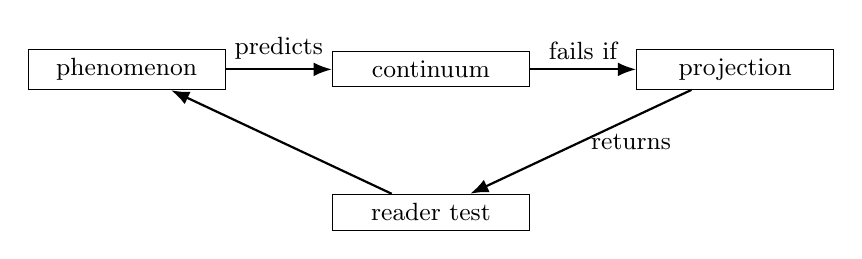
\begin{tikzpicture}[node distance=1.35cm,>=Latex,every node/.style={font=\small}]
\node[draw,align=center,minimum width=2.5cm] (c) {phenomenon};
\node[draw,align=center,minimum width=2.5cm,right=of c] (t) {continuum};
\node[draw,align=center,minimum width=2.5cm,right=of t] (f) {projection};
\node[draw,align=center,minimum width=2.5cm,below=of t] (r) {reader test};
\draw[->,thick] (c) -- node[above]{predicts} (t);
\draw[->,thick] (t) -- node[above]{fails if} (f);
\draw[->,thick] (f) -- node[right]{returns} (r);
\draw[->,thick] (r) -- (c);
\end{tikzpicture}
\caption{Basic Principle Must Work: falsifier of conceptual dependency pressure 27-1-22}
\label{fig:figure-why-the-basic-principle-must-work-at-minimal-substrate-one}
\end{figure}
The point of the diagram is not decoration; it marks which relation is being proposed and which stronger conclusion is still unavailable.\par
A local clarification is useful here\par
A local clarification is useful here\footnote{In Basic Principle Must Work, this note clarifies the reader clarification role of the term and keeps the caveat close to the sentence that needs it.}.\par
The note keeps the caveat near the term without derailing the main sentence.\par
Minimal substrate does not mean a hidden physical stuff underneath all things. It means the least set of descriptive distinctions required before the words system, change, constraint, incompatibility, continuation, expansion, and collapse can have determinate meaning. Without that substrate, the basic principle would be a slogan. With too much substrate, it would secretly import the furniture of one domain into every other domain. The problem is to find the level at which the principle can be stated without becoming either empty or imperial.\par
The cup helps because it is modest. It does not invite grandeur. Its boundary may be the ceramic wall, the surface between water and air, or the measurement interval chosen by an observer. Its continuity is the persistence of the described object across a change in temperature. Its operator is heat exchange with the surroundings. Its criterion of continuation is ordinary enough: the cup of water remains the cup of water while its thermal state changes. No claim about society, life, consciousness, or cosmic law is needed. The example shows only that even simple change requires a minimum structure of description.\par
The same need appears when the scene becomes more complicated. A bridge design must carry a load, fit a site, obey a budget, use available materials, and satisfy safety requirements. If those conditions cannot be jointly satisfied, the design faces an incompatibility. It may be abandoned, reduced, or replaced. It may also acquire a new axis of possibility: a different support geometry, a truss, an arch, a cable system, a staged maintenance model, or a new material relation. The basic principle tries to name this fork. But it can do so only if the configuration, constraints, boundaries, transformations, and criteria of success have already been made visible.\par
This is what the word must means in the chapter title. It is not a claim that nature has already been proved to obey one universal law. It is a descriptive necessity. If the basic principle is to mean anything across domains, it must be able to operate at the minimal level where changing configurations can be described. If it cannot work there, it cannot lawfully be carried upward into biology, institutions, language, computation, or formal theory. The minimal substrate is not a decorative beginning. It is the condition for the principle to have an object.\par
\section{One Principle, Many Projections In Basic Principle Must Work}
A system can be described in many domains: a cell in biology, a firm in economics, a storm in atmospheric science, a sentence in language, a legal institution in public life. Each domain has its own instruments, vocabulary, and standards of evidence. A cell membrane is not a statute. A statute is not an orbit. An orbit is not a sentence. Any theory that begins by erasing these differences has already lost the discipline needed to compare them. \cite{bertalanffy_general_system_theory,boulding_general_systems_theory}\par
The basic principle does not begin by claiming that all domains are secretly the same thing. It begins with a narrower question: what must a description contain before a domain can be represented as a changing configuration? That question can be asked without flattening the domains it touches. Measuring a membrane potential, interpreting a legal rule, modeling a planetary orbit, and analyzing a sentence remain different activities. What may recur is not their substance, but the descriptive need to mark boundaries, continuities, transformations, and failure conditions.\par
The local dependency can now be written without changing the claim it supports.\par
\begin{equation}\label{eq:equation-why-the-basic-principle-must-work-at-minimal-substrate-two}
\operatorname{caseCoverage}_{6} = \tau_{\mathrm{repair}}=\inf\{t:C(t)<\theta\}
\end{equation}
The relation names a local dependency, variable dictionary, and proof/evidence role; it is not a claim-status upgrade.\par
The formula is a restraint on the prose. It names the dependency that the surrounding paragraph is allowed to use.\par
The comparison below gives basic principle must work a set of quantities that can be inspected instead of merely admired.\par
\begin{table}[htbp]
\centering\small
\caption{Basic Principle Must Work: observable quantities and counter-pressure 27-2-22}
\label{tab:table-why-the-basic-principle-must-work-at-minimal-substrate-one}
\begin{tabular}{@{}llll@{}}
\toprule
Level & Axis pressure & Operator burden & Transition test \\
\midrule
basic principle must work boundary & 75 units & declared case & fixes what is compared \\
residual pressure & 0.84 & dimensionless & shows unresolved load \\
projection loss & 0.14 & bounded interval & marks lost structure \\
countercase set & 30 cases & review sample & keeps a falsifier visible \\
\bottomrule
\end{tabular}
\end{table}
The table should be read locally: it narrows the comparison without pretending that the wider theory has been settled by a single surface.\par
A domain is a field of description with its own objects, measures, and claims that can responsibly be made. A projection is a disciplined rendering of a general schema inside such a field. A system, in the plain introductory sense needed here, is an organized configuration that can be treated as having some persistence and relations among distinguishable aspects. These terms are not yet mathematical commitments. They are starting handles. They keep the inquiry from confusing a general language with the specialized evidence required by any particular field.\par
The history of general systems thought matters because it exposed both the attraction and the danger of this kind of language. Ludwig von Bertalanffy argued that living organization could not be understood well if every phenomenon were treated as a closed mechanical aggregate. Kenneth Boulding described levels of system organization to show why comparison across static structures, organisms, societies, and symbolic systems required more than local vocabulary. James Grier Miller looked for recurring process categories in living systems. Mesarovic and Takahara pushed toward more abstract system models and mathematical representation.\par
That lineage is useful here not as an authority to inherit whole, but as a warning. Cross-domain language is tempting because fields repeatedly encounter boundaries, inputs, outputs, feedback, persistence, breakdown, and reorganization. It is dangerous because words that travel too easily may stop explaining anything. The word system can become so broad that it merely signals intellectual ambition. A usable theory has to let vocabulary travel while refusing to treat travel as confirmation.\par
The cup, the bridge, and the school can be compared only under that restraint. A cup cooling on a table, a bridge design under load, and a school revising its admissions policy are not examples of one substance. They differ in matter, evidence, purpose, and standards of judgment. Yet each can be described as a configuration with boundaries, changing states, operators, and criteria of continuation. The commonality is a shared demand placed on description, not a shared mechanism already discovered in the world.\par
This distinction protects the scientific status of the argument. A cross-domain schema may be useful as a research program, a formal vocabulary, or a comparative tool. That does not make it an empirical law of nature. It does not prove that every domain is governed by one hidden mechanism. It does not license claims about data, experiments, simulations, or formal verification that have not been supplied. At this stage the claim is conceptual: later domain claims must be stateable without smuggling in a false unity at the start.\par
\section{Contradiction At Small Scale In Basic Principle Must Work}
Human intuition is comfortable at the scale of hands, rooms, roads, tools, and familiar institutions. Inquiry is not confined to that scale. It runs downward to molecules, cells, and fields; upward to planets, climates, and galaxies; sideways into economies, networks, languages, and computational systems. The world presented to description is not arranged at one privileged human size. \cite{bertalanffy_general_system_theory,boulding_general_systems_theory}\par
Astronomical continuity names this pressure from scale. The phrase is partly a teaching device and partly a technical reminder. It does not mean that the universe is smooth in every respect, or that all changes are gradual, or that discontinuities are unreal. It means that serious description repeatedly has to connect states across intervals larger, smaller, longer, shorter, or more complex than immediate appearance can hold. A star is not understood from one visible point of light. A climate is not understood from one afternoon. A culture is not understood from one utterance. A cell is not understood from one molecule alone.\par
The local dependency can now be written without changing the claim it supports.\par
\begin{equation}\label{eq:equation-why-the-basic-principle-must-work-at-minimal-substrate-one}
\operatorname{finiteCheck}_{6} = \operatorname{loss}_{\phi}=1-\frac{|E_{\phi}\cap E_{\mathrm{domain}}|}{|E_{\mathrm{domain}}|}
\end{equation}
The relation names a local dependency, variable dictionary, and proof/evidence role; it is not a claim-status upgrade.\par
The formula is a restraint on the prose. It names the dependency that the surrounding paragraph is allowed to use.\par
The local dependency can now be written without changing the claim it supports.\par
\begin{equation}\label{eq:equation-why-the-basic-principle-must-work-at-minimal-substrate-three}
\operatorname{counterexamplePressure}_{6} = I_{\mathrm{axis}}=\frac{\operatorname{Var}(x\mid a)}{\operatorname{Var}(x)}
\end{equation}
The relation names a local dependency, variable dictionary, and proof/evidence role; it is not a claim-status upgrade.\par
The formula is a restraint on the prose. It names the dependency that the surrounding paragraph is allowed to use.\par
A small numerical test keeps the abstraction honest at the scale of a single decision.\par
\paragraph{Numerical example.} For basic principle must work, take support=0.53, projection loss=0.11, and 2 open obligations. The bounded score is 0.140; the example gives the reader a numeric scale without pretending to be empirical proof.\par
The numbers are deliberately small; their value is pedagogical, not evidential, unless the chapter binds them to a dataset elsewhere.\par
The astronomical example is instructive because the sky taught scale discipline early. A planet seen from Earth appears as a wandering point. A fuller account treats it as a body with mass, orbit, atmosphere, history, and relation to a larger gravitational system. The object has not changed because the account has changed. The descriptive substrate has expanded. A point has been placed inside continuities that naked appearance could not supply.\par
Other fields undergo similar expansion. A symptom in medicine may begin as local discomfort, but explanation can connect it to tissue, circulation, immune response, behavior, and environment. A price change may appear as a number, but analysis may connect it to production, expectation, scarcity, regulation, and trust. A sentence may appear as a string of words, but linguistic description may connect it to grammar, convention, context, and intention. In each case, the immediately visible object is not enough.\par
Continuity must still be restricted or it becomes useless. If everything is connected to everything in the same way, explanation has not improved. A continuum, in the sense needed here, is a describable spread of possible variation along some aspect of a configuration. Temperature can vary. Load can vary. Membership can vary. Authority can vary in scope. Confidence in a claim can vary. These continua are not one continuum. They are comparable only in the limited sense that each requires variation to be marked, bounded, and transformed.\par
A boundary is the companion of continuity. It is a distinction that lets a description say what counts as inside, outside, adjacent, included, excluded, before, after, active, inactive, relevant, or irrelevant. Boundaries may be physical, as with a cell membrane. They may be institutional, as with membership rules. They may be conceptual, as with the difference between a hypothesis and a demonstrated result. They may be operational, as with a threshold at which a system changes behavior. A boundary is not always a wall. Often it is a rule for tracking difference.\par
The cup of hot water again shows why scale does not have to be grand to matter. At one scale, the cup is an object on a table. At another, it is a thermal system exchanging energy with its surroundings. The boundary of interest may be the cup wall, the water surface, the air around it, or the interval of measurement. The same ordinary object supports more than one legitimate description because the relevant boundary and continuum shift with the question being asked.\par
A general language has to survive such shifts without pretending that the same observables appear at every scale. The telescope, microscope, archive, sensor network, and formal model each reveal different aspects. A language that works only at one scale may be locally useful, but it cannot carry the burden of a general account of changing configurations. This is another reason the basic principle has to work at minimal substrate. Minimality is what lets the principle travel across scale without pretending that every scale is the same.\par
\section{When Dimension Becomes the Question In Basic Principle Must Work}
Broad theories often fail by confusing a principle with one of its projections. A principle is a general rule, form, or constraint stated at a level of abstraction. A projection is its expression inside a particular domain, instrument, model, or vocabulary. If the two are confused, the theory becomes either empty because it never reaches the world, or domineering because it treats one domain's vocabulary as the master language for all others. \cite{bertalanffy_general_system_theory,boulding_general_systems_theory}\par
The claim that organized configurations require boundaries is a principle-level claim. In a cell, its projection may involve membranes, channels, gradients, and transport. In a court, it may involve jurisdiction, procedure, standing, and admissible parties. In a software service, it may involve interfaces, permissions, runtime state, and failure modes. These are not interchangeable. A membrane is not a statute, and a statute is not an application programming interface. Yet each performs boundary work inside its own domain.\par
The case that follows turns the proposal into a sequence of criticizable moves.\par
\paragraph{Worked case.} In the worked case for basic principle must work, the claim is reduced to a boundary, an observable, a dependency, a numerical cue, and a falsifier. The case is useful only because each move can be criticized separately.\par
The case helps because each step can fail separately, which is exactly what a useful example should permit.\par
The basic principle must be read at this level before it is carried into any field: when a configuration contains an unresolved incompatibility among relevant constraints, it tends either to acquire a new dimension of description that permits reorganization, or to collapse relative to the criteria by which continuation was being described. This is not already a biological theorem, a sociological law, a physical equation, or a software architecture rule. It is a proposed schema for describing a certain kind of pressure in configurations.\par
The word contradiction needs care. In ordinary speech, contradiction can mean disagreement, hypocrisy, conflict, paradox, opposition, or formal inconsistency. Here it means an unresolved incompatibility inside a description of a configuration. The incompatibility may be logical, operational, structural, or normative, depending on the domain. What matters is that the current description cannot satisfy all relevant constraints at once without changing something important.\par
A compact counterexample helps. Two people in a room may prefer different paint colors. That is a conflict, but it is not yet a contradiction in the present sense. The room can be painted blue, green, striped, or not at all. The disagreement becomes a relevant incompatibility only if the description includes constraints that cannot be jointly satisfied, such as a binding rule that the room must be entirely blue, another binding rule that it must be entirely green, and no permitted way to partition, revise, or override the rules. Contradiction here is not mere difference. It is a failure of joint satisfaction under stated constraints.\par
The bridge case gives the stronger form. Suppose a proposed bridge must span a river, bear a specified load, use a specified material, meet a specified cost, and preserve a specified shape. If analysis shows that these conditions cannot be jointly satisfied, the design faces an unresolved incompatibility. One response is collapse: the design is abandoned, fails, or is reduced until it no longer serves the original purpose. Another response is expansion: the design introduces a new structural form, support geometry, material strategy, or maintenance regime. The new axis changes what can be done.\par
The school case shows why this is not only an engineering matter. A school may require open admission, small classes, low tuition, and broad curriculum. If resources make those conditions impossible together, the institution may contract, fail, or introduce a new dimension of organization: tiered scheduling, hybrid instruction, shared staffing, differentiated programs, or a new funding model. The content is social, not mechanical. The evidence is different. The standards are different. The shape of the pressure is still describable.\par
Analogy, schema, and evidence must be kept apart. An analogy says one case resembles another in some respect. A schema states a general form that can be projected into different cases. Evidence belongs to a domain and bears on whether a projected claim is true, useful, or false there. The cup, bridge, and school are not evidence that one universal law has been proved. They are examples that reveal the schema and show what a domain projection would have to specify.\par
A projected claim must take on local obligations. In physics it must respect measurement, mathematical law, and experimental discipline. In biology it must respect organism, environment, lineage, and observation. In social analysis it must respect institutions, interpretation, history, and normativity. In formal work it must respect definitions and derivations. A projection that cannot meet the obligations of its domain is not rescued by the elegance of the principle.\par
This separation also prevents premature dismissal. A poor projection in one field does not automatically refute every possible projection. A useful projection in one field does not certify the rest. Each carries its own burden. The ambition is therefore conditional and disciplined: to state a vocabulary capable of projection, not to bypass the work that projection requires.\par
\section{The Hypothesis In Plain Words In Basic Principle Must Work}
The bridge can now be used to derive the substrate rather than merely illustrate it. Before there can be a contradiction in the design, there must first be a configuration. The configuration is not every fact about the river, the city, the economy, or the materials industry. It is the proposed bridge as described for the purpose at hand: a planned arrangement of span, supports, materials, site, load requirements, cost limits, and safety expectations. \cite{bertalanffy_general_system_theory,boulding_general_systems_theory}\par
Second, the configuration must have distinguishable aspects. If span, load, material, cost, geometry, and exposure cannot be distinguished, no incompatibility among them can be stated. An undifferentiated mass cannot fail to satisfy multiple constraints because there are no articulated constraints to compare. Distinction is not optional ornament. It is the condition for saying that one aspect presses against another.\par
Third, there must be continuity through variation. A design may pass through revisions while still being treated as the same project. If every alteration produced an entirely new object with no continuity, then reorganization could not be distinguished from replacement. Continuity does not require sameness in every respect. It requires enough persistence across an interval for the description to track change as change of something.\par
Fourth, there must be boundaries. The bridge design is bounded by the river site, expected traffic, legal requirements, available budget, construction methods, environmental exposure, and the scope of the engineering question. Those boundaries can move, but they cannot be absent. Without boundaries, the description cannot say which constraints are relevant and which belong to another problem.\par
Fifth, there must be operators. An operator is anything that performs a transformation within a description. In the bridge case, calculation, material substitution, load testing, redesign, regulatory approval, and construction sequencing can function as operators. Operators need not be the same kind of thing in every domain. Heating can function as an operator in a thermal description. Mutation can function as an operator in an evolutionary description. A vote can function as an operator in an institutional description. A rule of inference can function as an operator in a formal description. The shared point is transformation under a description.\par
Sixth, there must be criteria for continuation and collapse. A bridge design continues, in the relevant sense, if it can still satisfy the purpose and standards under which it is being developed. It collapses as a design if it can no longer meet those standards, or if it is reduced into something that no longer counts as the intended bridge. Collapse here is not every alteration. It is failure of continuation relative to stated criteria.\par
The minimal substrate can now be summarized: configuration, distinguishable aspects, continuity through variation, boundaries, operators, and criteria of continuation or collapse. A seventh element is implicit in the relation among them: relevant constraints must be articulable, because incompatibility is always incompatibility among constraints. These elements do not amount to a complete science. They amount to the smallest ground on which the basic principle can be meaningfully asked.\par
The school example confirms the derivation in a different domain. The configuration is the institution. Its aspects include enrollment, staffing, curriculum, budget, legal obligations, community expectations, and time. Its continuity is the school persisting across years and policy revisions. Its boundaries include membership, jurisdiction, funding source, and educational mandate. Its operators include hiring, scheduling, policy change, curriculum redesign, tuition adjustment, and partnership. Its criteria include legal viability, educational function, financial solvency, and recognition by its community.\par
The point is not that a bridge and a school are the same kind of thing. They are not. The point is that the basic principle cannot even be posed in either case unless the same minimal kinds of descriptive work have been done. If no configuration is marked, there is nothing under pressure. If no aspects are distinguished, no incompatibility can be stated. If no continuity is tracked, reorganization cannot be separated from disappearance. If no boundaries are marked, relevance dissolves. If no operators exist, transformation has no place. If no criteria are stated, collapse and continuation become indistinguishable.\par
This also explains why the substrate must remain minimal. If it required physical membranes, it would exclude institutions and arguments too early. If it required conscious agents, it would exclude many biological, computational, and physical configurations. If it required formal equations from the beginning, it would exclude preliminary conceptual comparison. If it required only the claim that things change, it would be too thin to discipline anything. The substrate has to be strong enough to support the principle and weak enough not to decide every domain in advance.\par
\section{No Domain Wall Is Observed In Basic Principle Must Work substrat}
Dimensional birth is the phrase most likely to be misunderstood if it arrives too soon. It does not mean that a new physical dimension appears in space. It does not mean that reality expands whenever a problem becomes difficult. It means that a description acquires a new independent aspect, variable, level, or degree of freedom because the previous descriptive frame cannot resolve an incompatibility. \cite{bertalanffy_general_system_theory,boulding_general_systems_theory}\par
A dimension, in this introductory sense, is an axis of meaningful variation. Geometry gives the familiar case of length, width, and height, but the word is not limited here to spatial geometry. A budget introduces a dimension of cost. A legal system may introduce a dimension of jurisdiction. A biological model may introduce developmental timing as a dimension. A formal theory may introduce a distinction between syntax and semantics. A dimension lets a description vary in a way it could not previously vary.\par
Return to the bridge. The first design treats the span as a simple beam problem. Under load, the design cannot satisfy safety and cost constraints together. Spending more money may be a movement along an existing axis if cost was already part of the frame. Choosing a stronger grade of the same material may also remain within the old frame. But introducing truss geometry, cable support, arch action, modular segmentation, or a maintenance model that changes long-term fatigue assumptions may alter the design space itself. The new axis changes what counts as possible.\par
The word birth is used for that alteration of space, not for ordinary adjustment. If the school delays a decision by a week, it has not necessarily produced a new dimension. If it raises tuition within an already available budget model, it may only have moved along the cost axis. But if it creates a rotating schedule that changes the relation among enrollment, classroom capacity, staffing, and time, then time may become a new organizing dimension of the institution. What was impossible as a simultaneous arrangement may become possible as a temporal one.\par
This distinction is necessary because otherwise every solution could be called dimensional birth. The term must be held to local criteria. A serious claim of dimensional birth should identify the prior frame, the incompatibility inside it, the added axis, and the way that axis changes possible states. Without those elements, the phrase remains a metaphor. With them, it becomes an analyzable proposal within a domain.\par
Collapse is the paired term. Collapse means that a configuration can no longer continue under the description and criteria in force. It may be physical failure, institutional dissolution, loss of coherence in an argument, termination of a process, or reduction into a form that no longer satisfies the original configuration. It is not every change. A bridge design can change and continue. A school can change and continue. Collapse marks failure of continuation relative to stated criteria.\par
The basic principle names a fork under unresolved incompatibility. One path expands the descriptive space so that reorganization becomes possible. The other ends, abandons, breaks, or reduces the configuration that could not satisfy its constraints. The fork is not mystical. It is a disciplined way of asking what happens when the current frame cannot hold the demands placed on it.\par
The principle is valuable partly because it can be challenged in specific ways. A critic may show that the alleged incompatibility was not real. The added dimension may have been present all along. The configuration may not have collapsed but merely varied within an old frame. The criteria of continuation may have been poorly stated. The domain projection may lack measurable or otherwise admissible standards. These objections do not embarrass the theory. They keep it from becoming an all-purpose story.\par
The bridge and the school make the necessity argument visible. If dimensional birth and collapse are to be more than dramatic words, they require the substrate already derived. There must be a configuration to continue or fail, aspects that can become incompatible, boundaries that determine relevance, operators that transform the state, and criteria that distinguish reorganization from collapse. The basic principle must work at that minimal level because above it the vocabulary becomes domain-specific, and below it the vocabulary has no determinate use.\par
\section{One Principle, Many Projections In Basic Principle Must Work substrat}
The core hypothesis can now be stated without asking too much of the reader at once: when a configuration contains an unresolved incompatibility among its relevant constraints, the configuration tends either to acquire a new dimension of description that permits reorganization, or to collapse relative to the criteria by which its continuation was being described. \cite{bertalanffy_general_system_theory,boulding_general_systems_theory}\par
Every major word in that sentence has been prepared. A configuration is an organized arrangement under description. A constraint is a condition the configuration must satisfy or is being treated as subject to. An incompatibility is a failure of joint satisfaction among relevant constraints. A dimension is an axis of meaningful variation. Reorganization is a change made possible by an expanded descriptive space. Collapse is failure of continuation relative to stated criteria.\par
This is a metaontological proposal in a precise sense. A metaontology is a language for describing how descriptions themselves are organized: what kinds of entities, relations, boundaries, transformations, and failures a theory permits itself to name. The proposal is operational because it aims to make those permissions usable in analysis. It asks what has to be named for systems, continua, operators, boundaries, incompatibilities, emergent dimensions, and collapse to be compared without pretending that every domain has the same content.\par
Emergence enters here in a restrained sense. A feature emerges when a configuration displays a property, behavior, or descriptive necessity not available from the prior description of its parts alone. Dimensional birth is one possible way to describe an emergent need in explanation: the old frame cannot resolve the incompatibility, and a new axis becomes necessary for continued intelligibility. Whether a given case deserves that description depends on its projection and evidence.\par
The hypothesis explains why minimal substrate is not merely preliminary. Without the substrate, the hypothesis could be mistaken for a universal law of history, a psychological maxim, an engineering heuristic, or a metaphysical decree. With the substrate in view, it becomes narrower and more accountable. It applies only where configuration, aspects, constraints, boundaries, operators, continuity, incompatibility, and criteria of continuation can be specified. If those cannot be specified, the hypothesis may suggest a question, but it has not yet produced a claim.\par
A full scientific treatment would require more than this chapter supplies. It would need definitions tight enough for formal use, domain projections specific enough to be evaluated, and cases that do more than illustrate. It would need evidence, models, or derivations appropriate to each field. It would need comparison with rival accounts. It would need failures and limits. It would need procedures for deciding whether a proposed new dimension was genuinely new or merely renamed. None of that is being claimed here as already complete.\par
Still, the hypothesis has immediate intellectual value. It warns against treating contradiction only as a defect to be removed. In many descriptions, incompatibility is indeed an error. But in organized configurations, incompatibility can also reveal that the current descriptive frame is too poor. A system that cannot be understood under one set of distinctions may require another. The choice is not always between correct and incorrect statements inside a fixed frame. Sometimes the frame itself becomes the object under pressure.\par
The history of inquiry repeatedly shows this form of pressure, though each case has its own content. Scientific and formal fields often advance when conflict cannot be settled by choosing one old variable over another. New distinctions appear: energy separate from force, genotype separate from phenotype, syntax separate from semantics, computation separate from hardware implementation, weather separate from climate, legal authority separate from moral legitimacy. These examples do not prove the hypothesis. They show why the form is worth making explicit.\par
The hypothesis also preserves failure. Not every incompatibility yields richer organization. Some designs fail. Some institutions dissolve. Some arguments break. Some models are discarded. Some organisms die. Some research programs do not mature. Collapse is not an exception to the principle but one side of the fork it names. Any account that spoke only of creative expansion would be sentimental and false to ordinary experience.\par
The first burden of the chapter has therefore been met: the basic principle has been brought down to the smallest descriptive level at which it can have a stable meaning. It does not rest on a claim that all domains are one domain. It does not claim proof by analogy. It does not ask the reader to accept a hidden universal substance. It asks the reader to see that any serious account of configurations under unresolved incompatibility must begin with the minimal substrate that lets continuation, transformation, dimensional expansion, and collapse be distinguished.\par
From here the work can become more exact. The terms introduced in ordinary language can be sharpened: continuum, boundary, operator, projection, hierarchy, contradiction, emergence, collapse, and dimension. Their purpose is not to decorate the intuition, but to make it accountable. A principle that cannot descend to minimal substrate has no right to travel widely. A principle that can survive there has earned the next question: how far, and under what constraints, can it be projected?\par
\chapter{Dimensional Birth as the Central Intuition}
\section{No Domain Wall Is Observed In Dimensional Birth as Central}
Dimensional Birth begins with a refusal that is easy to miss. It does not begin by saying that physics, biology, psychology, institutions, and computation are secretly the same thing. It does not ask for a single master substance behind them, nor for a hidden equation already waiting beneath all observed differences. The first point is more modest and more severe: a system may change the kind of description required to keep it intelligible. When that happens, the change is not automatically a discovery of a new physical dimension, a new mathematical theorem, or a new empirical law. It is first a change in descriptive demand. \cite{boulding_general_systems_theory,miller_living_systems}\par
A first example can be taken from a familiar object: a city intersection. At one level, it can be described as geometry, with lanes, curbs, signal positions, and paths. At another level, it can be described as coordinated motion, with drivers, pedestrians, cyclists, timing, acceleration, and delay. At another level, it can be described as regulation, with right-of-way, enforcement, liability, and signage. None of these descriptions abolishes the others. The traffic light does not make geometry unreal, and the painted lane does not make law unnecessary. The intersection is not separated into sealed worlds. It is one practical situation that demands several kinds of description because different questions expose different operators, boundaries, and failures.\par
The next diagram slows the argument down just enough to show how dimensional birth as central is being organized.\par
\begin{figure}[htbp]
\centering
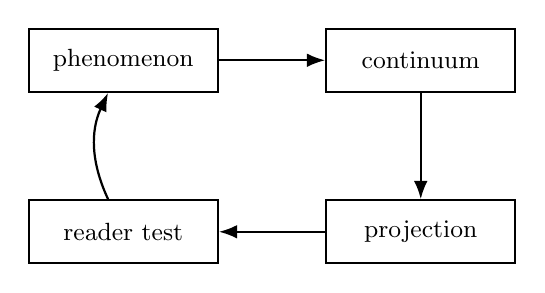
\begin{tikzpicture}[node distance=1.35cm,>=Latex,every node/.style={font=\small}]
\node[draw,thick,align=center,minimum width=2.4cm,minimum height=0.8cm] (a) {phenomenon};
\node[draw,thick,align=center,minimum width=2.4cm,minimum height=0.8cm,right=of a] (b) {continuum};
\node[draw,thick,align=center,minimum width=2.4cm,minimum height=0.8cm,below=of b] (c) {projection};
\node[draw,thick,align=center,minimum width=2.4cm,minimum height=0.8cm,left=of c] (d) {reader test};
\draw[->,thick] (a) -- (b);
\draw[->,thick] (b) -- (c);
\draw[->,thick] (c) -- (d);
\draw[->,thick,bend left=25] (d) to (a);
\end{tikzpicture}
\caption{Dimensional Birth as Central: state transition of conceptual dependency pressure 28-1-23}
\label{fig:figure-dimensional-birth-as-the-central-intuition-one}
\end{figure}
The point of the diagram is not decoration; it marks which relation is being proposed and which stronger conclusion is still unavailable.\par
A local clarification is useful here\par
A local clarification is useful here\footnote{In Dimensional Birth as Central, this note clarifies the reader clarification role of the term and keeps the caveat close to the sentence that needs it.}.\par
The note keeps the caveat near the term without derailing the main sentence.\par
The phrase domain wall will mean a barrier that would make one domain of description unreachable from another in principle. A no domain wall claim, in this limited sense, says that OC does not begin by declaring absolute walls between domains. It does not mean that all domains are interchangeable. It means that the movement from one descriptive register to another is a legitimate object of inquiry. The movement itself can be described: what had to be added, what had to be bracketed, what boundary became active, and what kind of contradiction forced the change.\par
This distinction matters because a theory of continua can fail in two opposite ways. It can flatten every domain into one vocabulary, losing the very differences that make biology unlike traffic engineering or law unlike thermodynamics. Or it can isolate each domain so completely that comparison becomes impossible. OC tries to occupy neither failure. It treats domains as regions of disciplined projection. A projection is a way of describing a system through selected observables, operators, and boundaries. A projection is not the whole system. It is a controlled view of the system.\par
General systems theory supplies a historical precedent for this posture without settling the present theory. Kenneth Boulding argued that scientific inquiry often advances by recognizing levels of organization rather than by forcing all phenomena into one level. James Grier Miller's work on living systems likewise treated different scales as organized by recurring processes while preserving the differences among cells, organs, organisms, groups, and societies. Mesarovic and Takahara gave general systems thinking a more formal vocabulary for system description and abstraction. Klir's architecture of systems inquiry emphasized that systems can be studied through multiple structured representations. These predecessors do not prove OC. They make intelligible why a monograph about continua can begin with comparison across domains without claiming that domain differences have disappeared.\par
\section{One Principle, Many Projections In Dimensional Birth as Central}
The second preparation concerns scale. OC uses the word continuum for a field of possible states, distinctions, or intensities along which a system can be described. A continuum is not necessarily a smooth physical line. It can be a structured range: stable to unstable, integrated to fragmented, explicit to implicit, reversible to irreversible, local to distributed, dormant to active. The important point is not smoothness but ordered variation. A continuum gives a system room to differ without requiring a new object name at every step. \cite{boulding_general_systems_theory,miller_living_systems}\par
Consider the night sky. A star-forming region, a mature star, a red giant, a white dwarf, and a supernova remnant are not interchangeable objects. They occupy very different physical states. Yet astronomy does not treat each state as an isolated vocabulary universe. It describes transitions, thresholds, conserved quantities, instabilities, collapse, radiation, and residual structures. This does not license loose metaphor. It illustrates a disciplined attitude toward continuity: large differences can be studied without pretending that each difference is a total break.\par
The local dependency can now be written without changing the claim it supports.\par
\begin{equation}\label{eq:equation-dimensional-birth-as-the-central-intuition-two}
\operatorname{transitionThreshold}_{6} = \rho_{\mathrm{replay}}=\frac{N_{\mathrm{matched}}}{N_{\mathrm{declared}}}
\end{equation}
The relation names a local dependency, variable dictionary, and proof/evidence role; it is not a claim-status upgrade.\par
The formula is a restraint on the prose. It names the dependency that the surrounding paragraph is allowed to use.\par
The comparison below gives dimensional birth as central a set of quantities that can be inspected instead of merely admired.\par
\begin{table}[htbp]
\centering\small
\caption{Dimensional Birth as Central: observable quantities and counter-pressure 28-2-23}
\label{tab:table-dimensional-birth-as-the-central-intuition-one}
\begin{tabular}{@{}llll@{}}
\toprule
Example & Parameter & Value & What changes \\
\midrule
dimensional birth as central boundary & 78 units & declared case & fixes what is compared \\
residual pressure & 0.00 & dimensionless & shows unresolved load \\
projection loss & 0.25 & bounded interval & marks lost structure \\
countercase set & 31 cases & review sample & keeps a falsifier visible \\
\bottomrule
\end{tabular}
\end{table}
The table should be read locally: it narrows the comparison without pretending that the wider theory has been settled by a single surface.\par
Astronomical continuity in this chapter is therefore not an astronomy thesis. It is a model of patience. The visible universe teaches that immense differences can be joined by lawful or partially lawful transitions, and that a descriptive system must often track both continuity and rupture. A star may remain the same object for practical naming across phases while requiring different equations, observables, and explanations at different phases. Identity and description do not always change at the same rate.\par
This matters for Dimensional Birth because the central intuition is not that a new dimension appears whenever a writer wants richer language. A new dimension of description is demanded only when the existing descriptive coordinates cannot account for the way a system continues, fails, transforms, or reorganizes. The new dimension must earn its place by doing work. It must distinguish cases that were previously confused, explain why an old description failed, and preserve what the old description still handled correctly.\par
A city again makes the point concrete. Suppose traffic engineers describe an intersection by vehicle flow alone. For ordinary commuting hours, the description may work well enough. Then a hospital opens nearby, emergency vehicles begin crossing the same junction, pedestrians increase, and delivery vehicles block curb lanes. The older description has not become false in every respect. Vehicle flow still matters. But a new axis may be required: priority under emergency constraint. Once that axis is introduced, the system can express cases that flow alone blurred together. A stopped vehicle may be congestion, compliance, hazard response, or lifesaving priority. The descriptive space has expanded because the system forced a distinction.\par
\section{Contradiction At Small Scale In Dimensional Birth as Central}
The third preparation is the difference between a principle and a projection. A principle is a general rule of description that the theory proposes across many cases. A projection is a domain-specific rendering of that rule into the terms, measurements, and boundaries available in one area. Confusing these two levels is one of the easiest ways to overstate a theory. If a principle is treated as though it were already a verified empirical result in every projection, the theory becomes inflated. If every projection is treated as unrelated, the principle becomes empty. \cite{boulding_general_systems_theory,miller_living_systems}\par
The relevant principle here is that unresolved contradiction can force a change in descriptive dimensionality. The word contradiction will not mean a mere disagreement between two people, nor every formal logical inconsistency. It means a structured incompatibility inside a system's current organization or description: two requirements, tendencies, constraints, or operations cannot be jointly maintained under the available coordinates. A bridge designed only for light pedestrian use faces such a contradiction when it becomes a route for heavy vehicles. The contradiction is not a mood. It is a mismatch between load, structure, use, and allowable deformation.\par
The local dependency can now be written without changing the claim it supports.\par
\begin{equation}\label{eq:equation-dimensional-birth-as-the-central-intuition-one}
\operatorname{operatorBurden}_{6} = G=(V_{\mathrm{claim}}\cup V_{\mathrm{evidence}},E_{\mathrm{support}}\cup E_{\mathrm{challenge}})
\end{equation}
The relation names a local dependency, variable dictionary, and proof/evidence role; it is not a claim-status upgrade.\par
The formula is a restraint on the prose. It names the dependency that the surrounding paragraph is allowed to use.\par
The local dependency can now be written without changing the claim it supports.\par
\begin{equation}\label{eq:equation-dimensional-birth-as-the-central-intuition-three}
\operatorname{graphWalk}_{6} = \epsilon_{\mathrm{domain}}=\max_i |y_i-\hat y_i|
\end{equation}
The relation names a local dependency, variable dictionary, and proof/evidence role; it is not a claim-status upgrade.\par
The formula is a restraint on the prose. It names the dependency that the surrounding paragraph is allowed to use.\par
A small numerical test keeps the abstraction honest at the scale of a single decision.\par
\paragraph{Numerical example.} For dimensional birth as central, take support=0.56, projection loss=0.16, and 3 open obligations. The bounded score is 0.100; the example gives the reader a numeric scale without pretending to be empirical proof.\par
The numbers are deliberately small; their value is pedagogical, not evidential, unless the chapter binds them to a dataset elsewhere.\par
A projection of this principle into engineering would use the quantities and tests appropriate to structures. A projection into institutional life would use roles, procedures, authority, incentives, and failure modes. A projection into biology would use viability, regulation, development, metabolism, or signaling. Each projection must respect its own evidence and methods. The principle does not carry the projection by force. It only proposes a pattern to investigate: when a system cannot resolve a structured incompatibility within its existing descriptive frame, either a new descriptive axis becomes necessary or the configuration fails.\par
The phrase dimensional birth names the first outcome. It does not mean that the universe has literally produced a new spatial dimension whenever a descriptive expansion occurs. It means that a new coordinate of intelligibility has become necessary for the system to be described without distortion. The phrase collapse names the second outcome. Collapse does not always mean physical destruction. It can mean loss of organization, loss of viability, loss of role coherence, loss of explanatory adequacy, or transition into a different regime where the former configuration no longer persists.\par
The objection is immediate: perhaps all such talk simply renames ordinary complexity. That objection has force. Many systems are complex without needing a new dimension of description. A machine with many parts is not automatically a case of Dimensional Birth. A long list of variables is not a theory. OC must distinguish multiplication from necessity. A dimension is not born because description becomes lengthy; it is born when a missing axis prevents the description from separating cases that behave differently under contradiction. If adding a term merely decorates the description, it is not a dimension. If adding it changes what can be predicted, compared, rejected, or explained, then the proposal becomes serious.\par
\section{When Dimension Becomes the Question In Dimensional Birth as Central}
Before the central intuition can carry later claims, the reader needs a minimal substrate: the smallest set of terms needed to follow the argument without importing a whole philosophical system. OC begins with systems, boundaries, continua, operators, contradictions, projections, emergence, and collapse. These words will later become more formal, but their initial meanings must be plain enough to use. \cite{boulding_general_systems_theory,miller_living_systems}\par
A system is a bounded organization of relations. The boundary may be physical, functional, legal, conceptual, computational, biological, or methodological. A cell membrane is a physical and biochemical boundary. A password system is a computational and authorization boundary. A court's jurisdiction is a legal boundary. A research model's assumptions form a methodological boundary. Boundaries do not merely separate inside from outside. They decide what interactions count as internal, external, permitted, blocked, transformed, or ignored.\par
The case that follows turns the proposal into a sequence of criticizable moves.\par
\paragraph{Worked case.} In the worked case for dimensional birth as central, the claim is reduced to a boundary, an observable, a dependency, a numerical cue, and a falsifier. The case is useful only because each move can be criticized separately.\par
The case helps because each step can fail separately, which is exactly what a useful example should permit.\par
A continuum is an ordered field of variation within which a system can occupy different states. Temperature is an obvious physical continuum. Trust in an institution is not measured in the same way, but it can still vary in ordered ways if the indicators are stated carefully. A theory that treats every continuum as identical loses precision. A theory that refuses to compare continua at all loses generality. OC uses continua as descriptive instruments, not as magic bridges among unlike sciences.\par
An operator is an action, rule, process, or transformation that changes a system's state along one or more continua. Heating water is an operator in a physical case. Changing a voting rule is an operator in an institutional case. Introducing a new feedback loop is an operator in a control system. Operators matter because systems do not merely sit in continua; they move, are moved, resist movement, or reorganize under operations.\par
Emergence is the appearance of a pattern, property, or behavior that is not adequately described by listing lower-level parts alone. The term has often been used vaguely, so OC treats it cautiously. Emergence is not an excuse to stop explaining. It is a signal that the relevant description may require a higher-order organization, a new boundary, or a new continuum. Collapse is the failure of a configuration to maintain the organization that made it that configuration. Collapse may be sudden or slow, catastrophic or quiet. A dissolved committee, a failed protocol, an unstable star, and a broken feedback loop are not the same phenomenon, but each can lose the organization by which it formerly operated.\par
With these terms in place, the central intuition can be stated without theatrical force: when a system is held between incompatible demands that cannot be resolved within its current descriptive coordinates, the next adequate description may require a new dimension. If such a dimension cannot be generated, stabilized, or projected, the configuration may collapse. This is not yet a demonstrated universal law. It is the guiding hypothesis that the rest of the monograph will discipline.\par
\section{The Hypothesis In Plain Words In Dimensional Birth as Central}
Dimensional Birth is the name for the transition in which a system's contradiction makes a new descriptive axis necessary. The word birth is intentionally stronger than addition. Many additions are optional. A useful label, a convenient category, or a more detailed measurement may improve a description without changing its basic dimensionality. Birth implies that the new axis is required because the old description cannot continue to do its job. \cite{boulding_general_systems_theory,miller_living_systems}\par
Return to the intersection. A simple traffic model may contain lanes, signal phases, vehicle counts, and average delay. It works until new pressures appear: emergency response, school crossings, delivery congestion, sensor failure, weather variation, and unequal risk among different users. At first, the model can absorb these as exceptions. Eventually the exceptions cease to be exceptional. The intersection is no longer adequately described by throughput alone. A new axis such as vulnerability, priority, or resilience may become necessary. The intersection has not become a different object in ordinary language. It has become a different object for explanation.\par
The same structure appears in less visible settings. A software service designed around request speed may later become responsible for privacy, auditability, and recovery after failure. Speed remains real. It no longer organizes the whole problem. A purely speed-centered description can even become dangerous if it hides the contradiction between fast response and accountable behavior. The system may require a new axis such as traceability. Once traceability enters, actions that previously looked identical become distinct: a fast response with recoverable record, a fast response without recoverable record, a delayed response caused by verification, and a blocked response caused by policy. The new axis changes the descriptive space.\par
The theory's discipline lies in refusing to call every improvement Dimensional Birth. A dimension must satisfy a stricter role. It must expose a difference that matters to the system's persistence, transformation, or failure. It must interact with operators. It must clarify boundaries. It must make some previous contradiction legible. It must also allow rejection. If the proposed dimension explains nothing that the old description could not already handle, it is ornamental. If it cannot be connected to any domain's observables or disciplined indicators, it remains speculative.\par
This is where the systems tradition is useful but not sufficient. Boulding's levels, Miller's living systems, Mesarovic and Takahara's formal systems language, and Klir's systems architecture all encourage careful movement between levels and representations. OC accepts that inheritance at the level of orientation. It then adds a sharper question: what forces a descriptive expansion rather than merely inviting one? Dimensional Birth is OC's answer in intuitive form. Contradiction is the pressure; a new dimension is one possible resolution; collapse is the alternative when the configuration cannot sustain the transition.\par
The objection again has to be answered plainly. Why not say simply that analysts add variables when they need them? Because variable addition is too weak to name the phenomenon at issue. A variable can be added inside an existing frame. Dimensional Birth concerns cases where the frame itself cannot distinguish the relevant states. In the traffic example, adding more vehicle counts may refine the old model but still miss emergency priority. In the software example, adding more latency metrics may refine the speed model but still miss traceability. A new dimension is not a larger spreadsheet. It is a new direction in which the system can differ.\par
\section{No Domain Wall Is Observed In Dimensional Birth as Central birthS06}
The core hypothesis can now be stated in its public form: an unresolved contradiction either gives rise to a new dimension of description or collapses the configuration that cannot resolve it. This sentence is not being presented as completed proof, settled empirical law, or finished mathematics. It is the organizing claim whose terms, limits, formal vocabulary, and domain projections have to be developed carefully. \cite{boulding_general_systems_theory,miller_living_systems}\par
The hypothesis has three moving parts. First, there must be an unresolved contradiction, not merely complexity, novelty, disagreement, or noise. Second, there must be a possible dimensional response: a new axis of description capable of making the contradiction intelligible without erasing the older valid descriptions. Third, there must be the possibility of collapse if the configuration cannot reorganize around the contradiction. These parts keep the hypothesis from becoming a slogan. They also give later analysis something to test against examples.\par
The hypothesis also explains why OC begins with intuition before formalism. A formal vocabulary introduced too early can make the argument appear more settled than it is. A reader must first see the kind of problem the vocabulary is meant to solve. The city intersection, the software service, and the astronomical analogy all point to the same underlying need: descriptions sometimes fail not because they are careless, but because the system has changed the dimensions along which adequacy must be judged.\par
There is no promise here that every domain will yield the same evidence, the same measurements, or the same standards of demonstration. A biological projection, an institutional projection, and a computational projection must each remain answerable to their own materials. The common theory is not a license to ignore domain knowledge. It is a way to ask a recurring question with controlled terms: when a system meets contradiction, does it generate a new dimension of organization or description, or does the configuration fail?\par
This prepares the handoff to the later architecture of the monograph. The next work is to sharpen the vocabulary, distinguish hierarchy from projection, show how continua and operators are represented, and separate intuitive plausibility from formal and empirical status. Dimensional Birth can carry later scientific claims only after it has been understood as a disciplined intuition: neither metaphor alone nor proof by announcement, but a proposed pattern of system transformation that must earn its authority wherever it is applied.\par
\chapter{Irresolvable Contradiction: New Dimension or Collapse}
\section{No Domain Wall Is Observed In Irresolvable Contradiction New Dimension}
A contradiction becomes philosophically interesting only after a simpler possibility has been removed. Perhaps the conflict is not in the world at all. Perhaps it has been produced by the vocabulary used to describe the world. Two descriptions may seem to collide because one belongs to biology and the other to mechanics, one to institutional life and the other to thermodynamics, one to internal experience and the other to public measurement. Before any theory earns the right to speak of contradiction, it must ask whether the apparent opposition is only a crossing of languages. \cite{miller_living_systems,mesarovic_takahara_general_systems}\par
OC, or operational continuum theory, begins with that restraint. It is not a theory of sameness. It does not claim that cells, courts, stars, minds, and formal systems are secretly one object under different names. It begins with a weaker and more useful claim: different regions of inquiry can sometimes be compared when the comparison is built from operations rather than imagery. An operation is something a configuration does or undergoes in a repeatable way: it exchanges, maintains, distinguishes, authorizes, excludes, repairs, transforms, or fails. If two cases can be compared at that level, the comparison may become disciplined. If they can only be compared by mood or metaphor, it has not yet earned theoretical weight.\par
The next diagram slows the argument down just enough to show how irresolvable contradiction new dimension is being organized.\par
\begin{figure}[htbp]
\centering
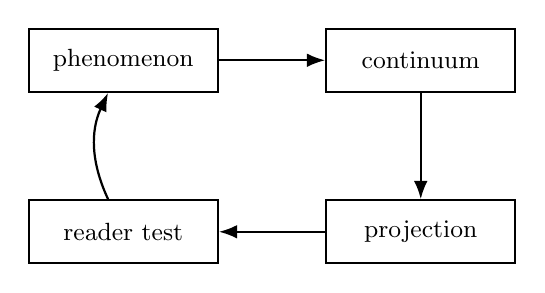
\begin{tikzpicture}[node distance=1.35cm,>=Latex,every node/.style={font=\small}]
\node[draw,thick,align=center,minimum width=2.4cm,minimum height=0.8cm] (a) {phenomenon};
\node[draw,thick,align=center,minimum width=2.4cm,minimum height=0.8cm,right=of a] (b) {continuum};
\node[draw,thick,align=center,minimum width=2.4cm,minimum height=0.8cm,below=of b] (c) {projection};
\node[draw,thick,align=center,minimum width=2.4cm,minimum height=0.8cm,left=of c] (d) {reader test};
\draw[->,thick] (a) -- (b);
\draw[->,thick] (b) -- (c);
\draw[->,thick] (c) -- (d);
\draw[->,thick,bend left=25] (d) to (a);
\end{tikzpicture}
\caption{Irresolvable Contradiction New Dimension: residual plot of conceptual dependency pressure 29-1-24}
\label{fig:figure-irresolvable-contradiction-new-dimension-or-collapse-one}
\end{figure}
The point of the diagram is not decoration; it marks which relation is being proposed and which stronger conclusion is still unavailable.\par
A local clarification is useful here\par
A local clarification is useful here\footnote{In Irresolvable Contradiction New Dimension, this note clarifies the reader clarification role of the term and keeps the caveat close to the sentence that needs it.}.\par
The note keeps the caveat near the term without derailing the main sentence.\par
A domain is a region of description in which certain questions, observables, and tests make sense. A cell, a market, a legal institution, a nervous system, and a star each have a domain of description. The word does not mean a separate universe. It means that each case admits some questions and resists others. A membrane potential is not a court ruling. A statute is not a metabolic pathway. A fusion process is not a deliberative procedure. The absence of identity is not a failure. It is the condition under which responsible comparison begins.\par
This is the first boundary OC places on itself: there is no absolute wall that forbids comparison across domains, but there is also no license to carry a word from one domain to another without carrying its operating conditions. If a boundary is being discussed in biology, the relevant operations may include exchange, closure, repair, and reproduction. If a boundary is being discussed in law, the relevant operations may include jurisdiction, recognition, enforcement, and appeal. The same word can travel only when the work it does is restated. Otherwise the word has merely changed scenery.\par
The point matters because apparent contradiction often arises from careless travel. A living cell can be described chemically as an open flow of matter and energy, while biologically it can be described as a self-maintaining unity. Those descriptions are not automatically rivals. They answer different questions. James Grier Miller's living systems theory is useful here because it refuses the comfort of a single observable. It treats living systems and organizations as structured wholes with multiple subsystems, flows, and processes. Maturana and Varela press from another direction. Their account of autopoiesis describes the living system as a unity produced and maintained by the network of processes that constitute it. OC does not inherit either account as settled authority, but their contrast teaches a necessary caution: difference between descriptions is not yet contradiction.\par
A real contradiction, in the sense required here, needs more than two sentences that sound opposed. It appears when a configuration cannot satisfy its own necessary operations under the description presently available. A configuration is a set of elements and relations considered together because their arrangement matters. The contradiction is not a literary tension or a disagreement of temperament. It is an obstruction in the way the arrangement works. A system must preserve a boundary and cross it in the same respect; it must remain closed enough to be itself and open enough to continue; it must treat an element as both inside and outside under the same rule; it must conserve an invariant while using the violation of that invariant as its next step. Only then does the conflict become serious for the theory.\par
Many apparent contradictions dissolve when the domain is specified. A government agency can be politically subordinate and legally independent in different respects. A scientific model can be false as a literal picture and useful as an approximation. A living organism can be materially continuous with its environment and organizationally distinct from it. These are not failures of thought. They are cases where distinction prevents confusion.\par
Other conflicts do not dissolve so easily. A developing organism must be stable enough to preserve identity and plastic enough to become what it is not yet. A society must preserve rules and revise rules through procedures authorized by those same rules. A scientific field must rely on standards of evidence while changing the instruments and concepts that define admissible evidence. In such cases, the contradiction cannot be dismissed as a vocabulary clash. It becomes pressure on the descriptive space itself.\par
OC treats that pressure as a hypothesis, not as a settled law. The claim is not that every unresolved conflict creates a new dimension, nor that every collapse has the same form across nature, mind, and culture. The claim is narrower: when a configuration cannot resolve a contradiction within its present axes of description, either a new axis of description becomes necessary or the configuration loses the organization that made the contradiction possible. That sentence is not a theorem. It is an instrument. It must be made exact enough to support, narrow, or reject.\par
\section{One Principle, Many Projections In Irresolvable Contradiction New Dimension}
The hypothesis is easiest to misunderstand when it is heard as a story about sudden novelty. A new dimension can sound like a miracle. Collapse can sound like catastrophe. Astronomy slows both reactions. Large-scale stellar change often occurs through continuity rather than interruption. A star does not become a red giant because an alien law enters the universe. It evolves under constraints that were already present: gravity, pressure, radiation, nuclear processes, mass, composition, and time. The visible form changes because the balance among operations changes. \cite{miller_living_systems,mesarovic_takahara_general_systems}\par
The astronomical case matters here not because stars are institutions, organisms, or minds. They are not. It matters because a star gives a clean example of a configuration whose continuing organization depends on opposed necessities. Gravity draws matter inward. Pressure and radiation resist inward compression. Energy production maintains a balance that is neither peace nor accident. The star exists as a maintained relation among tendencies that, taken separately, would not yield the same form. Its stability is not the absence of opposition. It is the temporary organization of opposition.\par
The local dependency can now be written without changing the claim it supports.\par
\begin{equation}\label{eq:equation-irresolvable-contradiction-new-dimension-or-collapse-two}
\operatorname{reviewClosure}_{6} = \kappa_{K_6}=\frac{b_{K_6}+s_{K_6}}{1+o_{K_6}+q_{K_6}}
\end{equation}
The relation names a local dependency, variable dictionary, and proof/evidence role; it is not a claim-status upgrade.\par
The formula is a restraint on the prose. It names the dependency that the surrounding paragraph is allowed to use.\par
The comparison below gives irresolvable contradiction new dimension a set of quantities that can be inspected instead of merely admired.\par
\begin{table}[htbp]
\centering\small
\caption{Irresolvable Contradiction New Dimension: observable quantities and counter-pressure 29-2-24}
\label{tab:table-irresolvable-contradiction-new-dimension-or-collapse-one}
\begin{tabular}{@{}llll@{}}
\toprule
Question & Observed cue & Local value & Reader use \\
\midrule
irresolvable contradiction new dimension boundary & 81 units & declared case & fixes what is compared \\
residual pressure & 0. & dimensionless & shows unresolved load \\
projection loss & 0.36 & bounded interval & marks lost structure \\
countercase set & 32 cases & review sample & keeps a falsifier visible \\
\bottomrule
\end{tabular}
\end{table}
The table should be read locally: it narrows the comparison without pretending that the wider theory has been settled by a single surface.\par
When the internal conditions change, the old balance may no longer hold. The exhaustion of one fuel regime does not merely add a new event to an unchanged description. It changes which relations must be tracked if the object is to remain intelligible. A description adequate for one phase may become inadequate for another because the dominant constraints have shifted. The problem is not that gravity and pressure have become mysterious. The problem is that their former relation no longer describes the operating configuration.\par
This is where the astronomical analogy belongs in a chapter about contradiction. It shows that a transition can be continuous with its underlying operations while still requiring a new description of their organization. The contradiction is not a verbal paradox imposed on the star from outside. It lies in the dependency of a maintained form on forces and processes whose balance can cease to preserve that form. When the prior equilibrium cannot be sustained, the object must either reorganize into another phase or lose the organization that made it that object.\par
Continuity prevents the transition from being mistaken for magic. A cloud of gas, a protostar, a main-sequence star, a giant, and a remnant are not unrelated objects pasted onto one another. They are phases in which different constraints dominate. Yet continuity does not erase the reality of transition. A later phase cannot be understood merely by repeating the description of an earlier one in a louder voice. The older terms remain, but their relation has changed.\par
OC uses the image carefully. It does not claim that social systems, organisms, and stars obey the same domain laws. It uses the astronomical case to discipline the imagination. If a contradiction leads to a new axis of description, that axis is not an arbitrary invention. It must answer to something already operative but not yet expressible in the older coordinates. The new description does not abolish the old terms. It shows where their previous arrangement no longer suffices.\par
A more familiar example can be kept deliberately modest. Consider a small institution founded to make decisions by unanimous agreement. At the beginning, unanimity may preserve trust, responsibility, and shared ownership. Everyone must consent because every decision belongs to everyone. The rule is not ornamental. It is the form of legitimacy.\par
As membership grows, the same rule begins to obstruct action. The institution must decide, but any decision requires universal consent. Universal consent becomes less likely as the decision environment becomes more complex. The mechanism that once preserved the institution begins to prevent the institution from acting. This is not merely a disagreement among members. It is a contradiction in the operating form: the mechanism of unity has become a mechanism of paralysis.\par
Several outcomes are possible. The institution may collapse as a decision-making body. It may fragment into smaller groups. It may introduce delegation, quorum rules, ranked procedures, appeal structures, or subject-specific authority. If it does the latter, a new axis of description has appeared. Authority is no longer only the act of the whole. It can now vary by office, mandate, time, subject, review, and recall. The old vocabulary of unanimous agreement cannot describe this change adequately. The institution now requires terms such as representation, scope, legitimacy, reviewability, and remedy.\par
The astronomical analogy helps again, but only at the level of disciplined structure. The institution has not left institutional reality and entered another universe. Its new procedure remains continuous with its prior need for legitimate decision. Yet the form of legitimacy has changed. The contradiction did not prove that unanimity was foolish. It revealed the condition under which unanimity ceased to be sufficient.\par
\section{Contradiction At Small Scale In Irresolvable Contradiction New Dimension}
A principle is not the same as a projection. A principle states a relation that may hold across more than one case when its conditions are met. A projection carries a pattern from one domain into another. Projection is not inherently wrong. It is how thought often begins. The error comes when projection is mistaken for principle before the receiving domain has been examined. \cite{miller_living_systems,mesarovic_takahara_general_systems}\par
The difference can be seen in the word collapse. In ordinary speech, collapse may mean a building falling, a government failing, a theory losing credibility, a market falling sharply, or a person losing composure. The shared word invites comparison. But if the comparison remains at the level of imagery, nothing has been learned. A building collapses through material failure under load. A government collapses through loss of authority, coordination, coercive capacity, legitimacy, or administrative continuity. A theory collapses when its explanatory structure can no longer handle decisive objections, anomalies, or internal inconsistency. These are not the same event.\par
The local dependency can now be written without changing the claim it supports.\par
\begin{equation}\label{eq:equation-irresolvable-contradiction-new-dimension-or-collapse-one}
\operatorname{sourceReliability}_{6} = \operatorname{support}(c_{6})=P(c_{6})\wedge E(c_{6})\wedge R(c_{6})
\end{equation}
The relation names a local dependency, variable dictionary, and proof/evidence role; it is not a claim-status upgrade.\par
The formula is a restraint on the prose. It names the dependency that the surrounding paragraph is allowed to use.\par
The local dependency can now be written without changing the claim it supports.\par
\begin{equation}\label{eq:equation-irresolvable-contradiction-new-dimension-or-collapse-three}
\operatorname{empiricalConstraint}_{6} = \operatorname{falsify}(h)=\exists e\in E\,:\,\operatorname{pred}_h(e)\neq\operatorname{obs}(e)
\end{equation}
The relation names a local dependency, variable dictionary, and proof/evidence role; it is not a claim-status upgrade.\par
The formula is a restraint on the prose. It names the dependency that the surrounding paragraph is allowed to use.\par
A small numerical test keeps the abstraction honest at the scale of a single decision.\par
\paragraph{Numerical example.} For irresolvable contradiction new dimension, take support=0.59, projection loss=0., and 4 open obligations. The bounded score is 0.100; the example gives the reader a numeric scale without pretending to be empirical proof.\par
The numbers are deliberately small; their value is pedagogical, not evidential, unless the chapter binds them to a dataset elsewhere.\par
OC uses collapse in a stricter sense. Collapse means the loss of the organization that allowed a configuration to function as that configuration. The definition is abstract, but it is not empty. It requires identification of the relevant organization, the operations that sustain it, and the conditions under which those operations cease to hold together. A bridge, a cell, an institution, and a formal model can all collapse, but the evidence for collapse differs in each domain.\par
The companion term dimension also needs discipline. Here a dimension is not necessarily a spatial direction. It is an axis of description along which differences can be registered and operations can be ordered. Temperature is a dimension in some physical descriptions. Authority can be a dimension in institutional descriptions. Closure can be a dimension in descriptions of living organization. A new dimension appears when the older axes cannot register a difference that has become operationally necessary.\par
Return to the institution governed by unanimity. Describing it only by member count and decision topics misses the critical change. The contradiction becomes visible when authority is introduced as an axis. At first, authority is undivided: the whole body authorizes each action. Later, the same undivided authority prevents timely action. Delegation introduces a new axis because authority can now vary by office, mandate, time, subject, reviewability, or recall. This is not decorative vocabulary. It allows distinctions that the original description could not make.\par
There is an obvious objection. Perhaps this is only a practical compromise described in grand language. The objection is healthy. OC earns its language only when the redescription changes what can be tested, inspected, or rejected. If the supposed new dimension adds no operational distinctions, it is only rhetoric. If it allows the system's transitions, failures, and recoveries to be described more accurately than before, then it has earned provisional use. Provisional is the important word. The theory does not ask for loyalty to the term. It asks whether the term makes the configuration more inspectable.\par
This distinction protects the hypothesis from opposite errors. One error treats every domain as so unique that no abstract comparison can survive. The other lets one domain supply metaphors for all the rest. OC rejects both. A principle must be abstract enough to travel and constrained enough to fail. A projection may suggest a principle, but it cannot certify one.\par
Maturana and Varela's autopoiesis offers an example of disciplined travel and its risks. The idea of a self-producing living unity has influenced discussions far beyond biology. Some of those extensions illuminate real structures. Others become loose metaphor. OC treats such movement cautiously. A concept can travel only if its operations are restated in the new domain. Self-production in a cell is not the same as self-description in a legal order or self-maintenance in an organization. Without that restatement, projection has outrun principle.\par
General systems theory offers a broader caution. Mesarovic and Takahara approached systems through formal relations, hierarchies, and abstract structures rather than through one preferred material domain. Klir emphasized the architecture of systems problems: how inquiry is organized, how systems are represented, and how different descriptions can be compared. Their usefulness lies less in authority than in method. They show that cross-domain language can be powerful only when its structure is explicit. OC follows that lesson by treating contradiction not as a mood, but as a relation among operations, constraints, boundaries, and possible descriptions.\par
\section{When Dimension Becomes the Question In Irresolvable Contradiction New Dimension}
A theory of contradiction must show not only where it applies, but where it fails. Without rejection conditions, every difficult situation could be redescribed as a hidden birth or a disguised collapse. That would make the hypothesis impressive and useless. The narrower discipline is more demanding: some apparent contradictions produce no new dimension and no collapse because they were never operational contradictions in the first place. \cite{miller_living_systems,mesarovic_takahara_general_systems}\par
Imagine a research group arguing over whether a model is simple or complex. One member calls it simple because it has few equations. Another calls it complex because it is hard to interpret. The disagreement may become heated. It may sound philosophical. But no contradiction has yet been established. The word simple is being used along two axes: formal size and cognitive accessibility. Once those axes are separated, the conflict dissolves. The model can be formally simple and interpretively difficult. No new dimension has been born in the strong sense, because the needed distinction was already available. No collapse has occurred, because the configuration was not unable to perform its necessary operations.\par
The case that follows turns the proposal into a sequence of criticizable moves.\par
\paragraph{Worked case.} In the worked case for irresolvable contradiction new dimension, the claim is reduced to a boundary, an observable, a dependency, a numerical cue, and a falsifier. The case is useful only because each move can be criticized separately.\par
The case helps because each step can fail separately, which is exactly what a useful example should permit.\par
The same pattern appears in ordinary institutional life. A rule may be called strict by one person because it is enforced consistently, and flexible by another because it allows many exceptions. The apparent contradiction may vanish when enforcement and scope are distinguished. A strict rule with broad exceptions is not impossible. It is merely underspecified until the relevant axes are separated. If the institution can continue to apply the rule after that clarification, the case does not belong to the core hypothesis.\par
This kind of failure is important. It shows that the hypothesis cannot be triggered by verbal opposition alone. The test is operational. What must the configuration do? Which operations are jointly required? Under what description do they conflict? Can the conflict be resolved by clarifying respects already available in the domain? If so, the case is not a birth of dimension or a collapse. It is an ordinary repair of description.\par
A second kind of rejection occurs when pressure damages a configuration without revealing a new axis or a structural contradiction. A committee may miss a deadline because too many members are absent. A machine may stop because a part breaks. A theory may be ignored because its readers are inattentive. These failures may be consequential, but consequence is not the same as contradiction. Unless the failure arises from jointly required operations that cannot be maintained under the current organization, the case remains outside the hypothesis.\par
Support for the hypothesis would therefore have a recognizable form. One would need to identify the configuration, its operations, its boundary distinctions, and its constraints; show that the contradiction is not merely verbal; show that existing axes cannot resolve it while preserving the configuration; and then show either that a new axis permits a more accurate account of transition or that the organization is lost. Narrowing would occur when a proposed case fails one of those steps. Rejection would occur if alleged dimensional births repeatedly add no operational distinctions, or if alleged collapses can be explained without contradiction in the required sense.\par
This makes the theory less dramatic, but more usable. It must be able to say no to its own temptation. A model that cannot distinguish discovery from relabeling, expansion from evasion, and collapse from ordinary failure has only changed the names of things. OC is valuable only if it sharpens the conditions under which those names are deserved.\par
\section{The Hypothesis In Plain Words In Irresolvable Contradiction New Dimension}
The hypothesis requires a minimal setting before the language of contradiction, dimension, or collapse is appropriate. Without such a setting, the theory would apply everywhere and explain little. The setting is not a hidden substance underneath all things. It is the least operational arrangement in which the relevant question can arise. \cite{miller_living_systems,mesarovic_takahara_general_systems}\par
First, there must be a configuration. A configuration is a set of elements and relations considered together because their arrangement matters. A pile of stones is a configuration if the arrangement affects load, access, meaning, or use. A sentence is a configuration because the order of words changes what can be said. A cell is a configuration because molecules, membranes, gradients, and processes are arranged in ways that sustain living organization. The term is broad, but not limitless. Where arrangement makes no difference, configuration has not yet entered.\par
Second, there must be operations. An operation is a repeatable transformation, maintenance activity, exchange, distinction, or rule-governed act within a configuration. Operations may be physical, biological, cognitive, institutional, or formal, depending on the domain. The theory does not require all operations to be measurable in the same way. It requires that the relevant operations be identifiable enough that failure, continuation, and change can be distinguished.\par
Third, there must be a boundary. A boundary is not merely a line. It is an operation of distinction that makes inside and outside, same and different, before and after, permitted and forbidden, or valid and invalid meaningful within a domain. A cell membrane is a boundary with material exchange. A legal jurisdiction is a boundary with institutional force. A formal definition is a boundary within a theory. Boundaries can be porous, layered, contested, or dynamic. What matters is that the configuration depends on some distinction being maintained.\par
Fourth, there must be constraint. A constraint limits what operations can occur while still preserving the configuration. Constraint is not only restriction; it is also the condition of form. A melody exists because not every note occurs at once. A living organism exists because chemical processes are organized rather than random. A scientific concept exists because some uses count and others do not. Without constraint, there is change but no determinate configuration to preserve or lose.\par
Fifth, there must be a way for contradiction to matter. A contradiction matters when jointly required operations cannot be satisfied under the current organization. If two preferences clash, there may be conflict but not yet operational contradiction. If two rules apply to the same case in incompatible ways, and the system must act, the contradiction becomes operational. If a boundary must both exclude and include the same element in the same respect, the configuration faces a more serious problem. The theory begins at that point, not before.\par
These conditions can be seen in the institutional example. The configuration is the decision-making body. The operations include proposal, consent, objection, decision, and implementation. The boundary distinguishes members from nonmembers and valid decisions from invalid ones. The constraint is unanimity. The contradiction appears when the same unanimity required for legitimate action prevents action under conditions where action is necessary. Collapse means the body can no longer function as the decision-making body it was. Dimensional birth means that a new axis, such as delegated authority, becomes necessary to preserve function.\par
They can also be seen in the biological case, if approached carefully. A living system must maintain itself across exchanges with its environment. If it were sealed absolutely, it could not continue the material processes on which it depends. If it were open without organization, it would lose the unity that makes it a living system. The terms closed and open therefore cannot be treated as simple opposites. Autopoiesis made this tension central by describing living systems as organizationally closed while materially and energetically engaged with their surroundings. OC reads this not as proof of itself, but as an example of why a new axis may be required: closure in one respect and exchange in another must be distinguished before the apparent contradiction can be handled.\par
The minimal setting also clarifies what OC is not claiming. It is not claiming that every disagreement is a contradiction. It is not claiming that every new label is a new dimension. It is not claiming that every failure is collapse. It is not claiming that biology, astronomy, law, and formal systems share one material mechanism. It proposes a disciplined vocabulary for cases where configurations, operations, boundaries, and constraints can be identified, and where unresolved contradiction either forces a richer description or destroys the organization at stake.\par
\section{No Domain Wall Is Observed In Irresolvable Contradiction New Dimension hypothes}
Dimensional birth is the most easily inflated term in the hypothesis, so it must be kept close to examples. A dimension is born when the descriptive space must acquire a new axis to register an operational difference that has become unavoidable. The birth is not psychological excitement, cultural novelty, or conceptual decoration. It is the appearance of a necessary distinction. \cite{miller_living_systems,mesarovic_takahara_general_systems}\par
In the institution example, delegation is not merely a policy preference. It introduces a difference between the authority of the whole and the authority of an authorized part. Once that difference exists, questions become possible that could not previously be asked with precision. Who may decide? On what matter? For how long? Under what review? With what remedy if authority is exceeded? These questions mark the new axis. The original unanimity model did not contain them as internal distinctions. It treated legitimate decision as the act of the whole. The contradiction forced a richer space.\par
In the biological example, the new axis separates forms of closure and forms of exchange. Open versus closed is too crude when the system depends on both. A new description appears when the opposition is decomposed into material exchange, organizational closure, boundary maintenance, and process reproduction. The contradiction does not disappear by verbal trick. It becomes tractable because the descriptive space now matches more of the system's operating structure.\par
A formal theory can undergo a similar transition. A concept may work until it is asked to handle cases at a new level of abstraction. At first, a category may be treated as fixed. Later, the theory may need to distinguish object-level use from meta-level description. Without that distinction, statements about the system become tangled with statements inside the system. The new dimension is not a new physical direction. It is a level distinction that prevents collapse of use and mention, rule and commentary, object and description.\par
Again, the claim is not that institutional delegation, living organization, and formal hierarchy share one mechanism. They do not. The claim is that unresolved contradiction often marks the insufficiency of an older descriptive space. The same pattern can be examined only if each domain supplies its own operations. Authority must be studied as authority. Closure must be studied through living organization. Formal levels must be studied through the rules of the theory. The comparison comes after the operational work, not before it.\par
Dimensional birth has a cost. Every new axis increases expressive power, but it also increases the burden of discipline. More distinctions can clarify; they can also conceal confusion. A theory that answers every problem by adding another dimension becomes unfalsifiable in practice. OC therefore treats dimensional birth as a constrained move. The new axis must be tied to an operational difference. It must explain why the previous axes failed. It must preserve continuity with the underlying operations. It must make some future error more visible, not less.\par
This cost is why collapse remains part of the central hypothesis. Not every contradiction is resolved by richer description. Some configurations cannot survive the conflict that exposes them. The unanimous institution may fail before delegation is accepted. A biological organization may lose the processes that maintained it. A theory may fragment into incompatible uses. Collapse is not the opposite of dimensional birth in a moral sense. It is the alternative outcome when the configuration cannot reorganize around the contradiction.\par
The pair matters because it avoids optimism disguised as theory. Emergence is often narrated as upward motion: more complexity, richer order, greater integration. OC does not assume that trajectory. It allows emergence, but it keeps failure in the frame. An unresolved contradiction may disclose a new dimension; it may also destroy the arrangement that made disclosure possible. The same pressure that reveals a missing axis can exceed the system's capacity to reorganize.\par
The term birth should therefore be heard soberly. It names the arrival of a distinction without which the configuration can no longer be adequately described. Sometimes that arrival is deliberate, as when an institution designs a new office. Sometimes it is retrospective, as when a field recognizes that an older opposition had concealed several different operations. Sometimes it is never stabilized at all. A possible dimension may appear as a need and vanish because the configuration collapses before the distinction can be made durable.\par
\section{One Principle, Many Projections In Irresolvable Contradiction New Dimension hypothes}
The core hypothesis can now be stated without theatrical force: when a configuration organized by identifiable operations, boundaries, and constraints encounters an irresolvable contradiction within its current descriptive dimensions, the outcome is either dimensional birth or collapse. Dimensional birth means that a new axis of description becomes necessary to preserve and understand the configuration. Collapse means that the configuration loses the organization by which it functioned as that configuration. \cite{miller_living_systems,mesarovic_takahara_general_systems}\par
The word irresolvable is the strictest word in the sentence. It does not mean difficult, emotionally troubling, politically inconvenient, or not yet solved by a particular observer. It means that the contradiction cannot be resolved while preserving the current dimensions and necessary operations of the configuration. This status is always relative to a description. A contradiction judged irresolvable under one vocabulary may become resolvable after distinctions are added. That is not a weakness in the hypothesis; it is the pattern being examined.\par
The hypothesis therefore has built-in humility. It does not pronounce from outside all domains. It asks a sequence of questions. What is the configuration? What operations sustain it? What boundary distinctions matter? What constraints preserve its form? Where is the contradiction located? Why can the current dimensions not resolve it? What would count as a new axis rather than a new name? What would count as collapse rather than ordinary change? Each answer can be challenged. That challenge is part of the theory's discipline.\par
The historical background helps locate the ambition. Miller's living systems theory shows how organized life and organized social forms can be described through multiple interacting subsystems without reducing them to a single observable. Maturana and Varela show how living unity can be approached through the processes that produce and maintain it. Mesarovic and Takahara show how systems can be studied through formal relations and hierarchies that are not confined to one material domain. Klir shows why the architecture of a systems problem matters: the description itself has structure, and that structure can clarify or distort what is being observed. OC belongs near these attempts to think organized complexity without flattening it, but it makes contradiction the hinge.\par
A continuum, in OC, is a range across which a configuration can vary while still being described in relation to some organizing concern. Stability and plasticity can form a continuum in developmental contexts. Openness and closure can form a continuum only after their respects have been specified. Authority can form a continuum from direct collective decision to delegated office. A continuum is not a vague spectrum. It is a structured range of possible differences. Contradiction becomes severe when movement along the available continua cannot preserve the configuration's necessary operations.\par
An operator is a repeatable rule or transformation that moves, maintains, distinguishes, or reorganizes a configuration within a continuum. Consent can be an operator in an institution. Exchange can be an operator at a boundary. Definition can be an operator in a formal system. Operators matter because contradictions are not merely static incompatibilities. They often appear when operations are applied and the configuration cannot continue coherently. A rule that once preserved order may, under changed conditions, generate disorder. An operator that once maintained identity may begin to undermine it.\par
The scientific status of the hypothesis depends on how those terms behave under pressure. It gains support when cases can be described in operational detail, when the alleged contradiction cannot be removed by ordinary clarification, when a new axis predicts or explains transitions that were previously obscure, and when collapse can be identified as loss of organization rather than mere inconvenience. It must be narrowed when a domain supplies better local terms, when the supposed contradiction is only a mismatch of scale, or when the proposed axis adds no testable distinction. It should be rejected where it cannot fail.\par
That final condition is essential. A hypothesis about contradiction must itself tolerate contradiction from evidence. If every failure becomes a secret success, if every criticism becomes proof of depth, if every unclear case is declared a new dimension, the theory collapses into projection. Its public value depends on the opposite discipline: the willingness to say that many conflicts are ordinary disagreements, many failures are ordinary failures, many analogies are only analogies, and many new names do not name new dimensions.\par
The result is a narrow but fertile starting point. A reader does not need to accept OC as true in order to see the problem it names. Contradiction can be more than inconsistency in language. Collapse can be more than dramatic failure. Dimension can mean an operational axis rather than a spatial direction. Continuity across domains need not imply identity of domains. Once those distinctions are in place, the title of the chapter becomes less like a slogan and more like a question: when a configuration meets a contradiction it cannot resolve on its own terms, does the world of description become wider, or does the configuration that needed description come apart?\par
No answer can be given in advance for every domain. The fork must be found case by case, through operations, boundaries, constraints, and evidence. Sometimes the apparent contradiction will dissolve. Sometimes the configuration will break. Sometimes a new axis will become visible because without it the case cannot be described at all. The work of the theory begins in that difficult middle space, where restraint and imagination have to operate together.\par
\part{formalization path}
\chapter{Contradiction as a Recurrent Scientific and Philosophical Motif}
\section{No Domain Wall Is Observed In Contradiction as Recurrent Scientific}
Contradiction enters science first as an experience before it becomes a formal problem. Something does not sit still under the name that has been given to it. A measurement repeats, yet the explanation that should receive it begins to fray. A system appears stable when viewed from one distance and unstable when viewed from another. A cell maintains its own identity only by exchanging matter and energy with what it is not. A political order preserves continuity by changing its rules. In such cases the difficulty is not always that someone has made a simple mistake. Often the more interesting difficulty is that two descriptions, each locally useful, cannot be held together without strain. \cite{mesarovic_takahara_general_systems,klir_architecture_systems}\par
The word contradiction must be handled with care because it has several lives. In ordinary speech it can mean hypocrisy, inconsistency, reversal, or surprise. In formal logic it has a stricter sense: a proposition and its negation cannot both be true in the same system under the same interpretation. Philosophy has given the term still other roles, especially in accounts of change, negation, opposition, and becoming. Science usually approaches the matter more cautiously. It does not need drama. It needs to know whether the trouble comes from error, from inadequate measurement, from a model pushed beyond its range, from a real transition in the phenomenon, or from a deeper failure in the conceptual scheme.\par
The next diagram slows the argument down just enough to show how contradiction as recurrent scientific is being organized.\par
\begin{figure}[htbp]
\centering
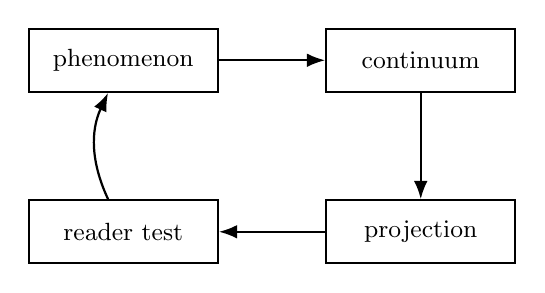
\begin{tikzpicture}[node distance=1.35cm,>=Latex,every node/.style={font=\small}]
\node[draw,thick,align=center,minimum width=2.4cm,minimum height=0.8cm] (a) {phenomenon};
\node[draw,thick,align=center,minimum width=2.4cm,minimum height=0.8cm,right=of a] (b) {continuum};
\node[draw,thick,align=center,minimum width=2.4cm,minimum height=0.8cm,below=of b] (c) {projection};
\node[draw,thick,align=center,minimum width=2.4cm,minimum height=0.8cm,left=of c] (d) {reader test};
\draw[->,thick] (a) -- (b);
\draw[->,thick] (b) -- (c);
\draw[->,thick] (c) -- (d);
\draw[->,thick,bend left=25] (d) to (a);
\end{tikzpicture}
\caption{Contradiction as Recurrent Scientific: concept map of conceptual dependency pressure 30-1-25}
\label{fig:figure-contradiction-as-a-recurrent-scientific-and-philosophica-one}
\end{figure}
The point of the diagram is not decoration; it marks which relation is being proposed and which stronger conclusion is still unavailable.\par
A local clarification is useful here\par
A local clarification is useful here\footnote{In Contradiction as Recurrent Scientific, this note clarifies the reader clarification role of the term and keeps the caveat close to the sentence that needs it.}.\par
The note keeps the caveat near the term without derailing the main sentence.\par
Consider a glass of water cooling toward freezing. At ordinary room temperature, it can be described with the vocabulary of a liquid. It flows, takes the shape of its container, and returns a smooth surface after disturbance. Lower the temperature, however, and the same material approaches a boundary where that vocabulary becomes incomplete. Near the transition, the language of liquid behavior still applies in important respects, but molecular ordering begins to matter in a new way. The difficulty is not that water is logically both liquid and solid in the same respect. The difficulty is that one descriptive frame is losing its authority over a changing organization.\par
This modest example already separates several things that are often confused. There may be an empirical anomaly: a measured result that does not match expectation. There may be descriptive strain: the old vocabulary still works but only awkwardly. There may be axis confusion: two observers may appear to disagree because one is speaking about flow while another is speaking about molecular order. There may be a regime transition: the system crosses a boundary at which old predicates no longer apply in the same way. There may also be system failure, where an organization can no longer maintain itself. These are not identical events. Calling them all contradiction would blur the very distinctions that make the phenomenon intelligible.\par
Scientific work depends on stabilized vocabularies. Object, state, variable, boundary, cause, equilibrium, function, and mechanism are not merely words; they are instruments of attention. They tell the observer what counts as relevant, what can be measured, what may be ignored, and what would count as an explanation. Their power comes from restriction. Yet the same restriction can become a source of blindness when a phenomenon changes level, crosses a threshold, or demands a second mode of description. The vocabulary that made inquiry possible can later become the thing that prevents inquiry from advancing.\par
General systems theorists saw this problem with unusual clarity. Mesarovic and Takahara treated systems not as isolated objects exhausted by a single picture, but as organized wholes that can be described through mappings, relations, and transformations. Klir emphasized that a system can be represented through alternative but disciplined views, with variables, levels, and relations specified rather than assumed. The point is not that these traditions make contradiction disappear. Their importance lies in making it legitimate to ask how a phenomenon changes when the descriptive apparatus changes.\par
That question belongs to both science and philosophy. Aristotle's principle of non-contradiction guards the conditions of intelligible predication: the same thing cannot both be and not be in the same respect at the same time. Hegel, by contrast, made contradiction central to the movement of concepts, though in a sense quite different from formal inconsistency. Modern science cannot simply inherit either posture without translation. It cannot abandon logical discipline, but it also cannot deny that many advances begin when an inherited description ceases to contain its object smoothly. The challenge is to preserve the precision of logic while acknowledging the productive pressure of mismatch, transition, and opposition.\par
In this book, contradiction is used in a restricted way. It does not mean every tension, every disagreement, or every surprising result. It names a patterned encounter between descriptions, levels, or operations that cannot be reconciled by ordinary correction while preserving the same descriptive situation. Sometimes the result is a better distinction. Sometimes it is a new variable, a new level, or a new model. Sometimes it is simply the collapse of a claim that cannot be saved. Nothing in the word itself guarantees discovery. The word marks a pressure point where the current way of saying what a system is no longer matches what the system is doing.\par
\section{One Principle, Many Projections In Contradiction as Recurrent Scientific}
The first task is to slow down the moment of strain. A contradiction in this restricted sense is not the same as an error. If a thermometer is broken, the discrepancy between expected and recorded temperature may be solved by replacing the instrument. If a calculation is wrong, the remedy may be arithmetic. If a term has been used ambiguously, the difficulty may dissolve once the ambiguity is removed. These cases matter because they protect inquiry from inflated language. Not every discomfort in thought deserves the name contradiction. \cite{mesarovic_takahara_general_systems,klir_architecture_systems}\par
A more difficult case arises when the instruments are working, the calculations are sound, and the terms have been used carefully, yet the phenomenon still resists the available description. At that point inquiry must ask whether the chosen boundaries, variables, or levels are adequate. The system may have been described too narrowly. The wrong relation may have been treated as central. A threshold may have been mistaken for a small variation within an unchanged field. What first appears as a defect in the world may turn out to be a defect in the description.\par
The local dependency can now be written without changing the claim it supports.\par
\begin{equation}\label{eq:equation-contradiction-as-a-recurrent-scientific-and-philosophica-two}
\operatorname{massGapToy}_{7} = C_{\mathrm{unres}}=\min_{\pi\in\Pi}\|B(x)-B(\pi x)\|
\end{equation}
The relation names a local dependency, variable dictionary, and proof/evidence role; it is not a claim-status upgrade.\par
The formula is a restraint on the prose. It names the dependency that the surrounding paragraph is allowed to use.\par
The comparison below gives contradiction as recurrent scientific a set of quantities that can be inspected instead of merely admired.\par
\begin{table}[htbp]
\centering\small
\caption{Contradiction as Recurrent Scientific: observable quantities and counter-pressure 30-2-25}
\label{tab:table-contradiction-as-a-recurrent-scientific-and-philosophica-one}
\begin{tabular}{@{}llll@{}}
\toprule
Boundary & Measured cue & Scale & Failure sign \\
\midrule
contradiction as recurrent scientific boundary & 84 units & declared case & fixes what is compared \\
residual pressure & 0.14 & dimensionless & shows unresolved load \\
projection loss & 0.47 & bounded interval & marks lost structure \\
countercase set & 33 cases & review sample & keeps a falsifier visible \\
\bottomrule
\end{tabular}
\end{table}
The table should be read locally: it narrows the comparison without pretending that the wider theory has been settled by a single surface.\par
The freezing of water shows this in elementary form, but the history of science offers stronger examples. In the late nineteenth century, blackbody radiation presented a crisis for classical physics. A heated cavity emits radiation across a spectrum of wavelengths. Classical reasoning could describe parts of the spectrum, but when extended across the whole field it led to an impossible result: energy should grow without bound at high frequencies. The problem was not a single bad observation. Nor was it merely a rhetorical tension between old and new language. It was a disciplined failure inside an otherwise powerful theoretical frame.\par
Planck's response did not simply repair a local detail. By introducing energy elements proportional to frequency, he opened the path toward quantum theory. The contradiction, if the word is used here, did not magically cause a new dimension of science to appear. Rather, the persistent failure of classical description forced a change in what could count as a physical state, a physical process, and an admissible explanation. The old frame could not keep all its commitments together: continuity, equipartition, observed spectra, and finite energy could not be preserved at once. Something had to give.\par
This case helps distinguish anomaly from contradiction. An anomaly is a result that conflicts with expectation. It may remain isolated. It may be absorbed by an auxiliary assumption. It may disappear with better measurement. A contradiction in the stronger descriptive sense appears when the anomaly exposes commitments that cannot all be maintained within the same explanatory frame. The pressure is then not only between observation and theory, but within the structure of the theory's own claims about what kinds of things and transformations are possible.\par
Axis confusion is another common source of false contradiction. In biology, the claim that a living organism is open seems obvious: it takes in nutrients, expels waste, exchanges heat, and responds to environmental conditions. Yet another claim also seems necessary: an organism is not merely an open stream of materials. It maintains a form of organization that distinguishes it from its surroundings. If openness and closure are treated as opposite positions on a single line, living systems look paradoxical. They seem open and closed at once.\par
Maturana and Varela's account of autopoiesis clarifies the matter. A living cell is materially open because substances and energy pass through it. It is operationally closed in the sense that its network of processes produces and maintains the organization that makes it a cell. Closure here does not mean isolation. It means that the organization of the system is constituted through a recursive network of operations. Varela's later work on autonomy sharpened this distinction: the organism remains coupled to an environment, but its identity is not simply imposed from outside.\par
Once the axes are separated, the apparent contradiction changes character. Exchange and organization are not the same direction of variation. A cell can be open with respect to matter and energy while closed with respect to the organization of its operations. The tension was real, but its form was misread. It did not require the abandonment of logic. It required a better description of the respect in which each claim was being made. Aristotle's old caution, often overlooked in casual uses of contradiction, returns here with force: the same thing, in the same respect, at the same time. Much confusion enters when the phrase in the same respect is forgotten.\par
\section{Contradiction At Small Scale In Contradiction as Recurrent Scientific}
A system is not first of all a thing with a sacred border. It is an organized object of inquiry whose components, relations, states, or operations can be distinguished from a surrounding context for some purpose. A thermostat, a cell, a laboratory apparatus, a river basin, an institution, and a mathematical model can all be treated as systems if the inquiry specifies what is being tracked and how the distinction from the environment is being drawn. This operational modesty is essential. Without it, the word system becomes either mystical or empty. \cite{mesarovic_takahara_general_systems,klir_architecture_systems}\par
The boundary is where much of the trouble begins. Some boundaries are material, such as the membrane of a cell or the wall of a vessel. Some are instrumental, such as the range and resolution of a measuring device. Some are conceptual, such as the decision to describe an economy through market prices rather than through unpaid household labor, ecological extraction, or informal exchange. A boundary is never innocent. It decides what can appear inside the account and what will be treated as background.\par
The local dependency can now be written without changing the claim it supports.\par
\begin{equation}\label{eq:equation-contradiction-as-a-recurrent-scientific-and-philosophica-one}
\operatorname{predictionWindow}_{7} = \Delta d=\operatorname{rank}(A_{\mathrm{new}})-\operatorname{rank}(A_{\mathrm{old}})
\end{equation}
The relation names a local dependency, variable dictionary, and proof/evidence role; it is not a claim-status upgrade.\par
The formula is a restraint on the prose. It names the dependency that the surrounding paragraph is allowed to use.\par
The local dependency can now be written without changing the claim it supports.\par
\begin{equation}\label{eq:equation-contradiction-as-a-recurrent-scientific-and-philosophica-three}
\operatorname{primeDeviationToy}_{7} = P_{\mathrm{collapse}}=\sigma(\alpha R-\beta S-\gamma M)
\end{equation}
The relation names a local dependency, variable dictionary, and proof/evidence role; it is not a claim-status upgrade.\par
The formula is a restraint on the prose. It names the dependency that the surrounding paragraph is allowed to use.\par
A small numerical test keeps the abstraction honest at the scale of a single decision.\par
\paragraph{Numerical example.} For contradiction as recurrent scientific, take support=0.42, projection loss=0.14, and 5 open obligations. The bounded score is 0.; the example gives the reader a numeric scale without pretending to be empirical proof.\par
The numbers are deliberately small; their value is pedagogical, not evidential, unless the chapter binds them to a dataset elsewhere.\par
Contradiction often announces that a boundary has become too narrow. A model of a lake as a chemical reservoir may work for certain questions about concentration and flow. It may fail when biological feedbacks, sediment interactions, seasonal turnover, and human intervention become decisive. A model of a disease as an invading pathogen may be indispensable, yet inadequate if immune response, social exposure, and ecological conditions are excluded. The issue is not that earlier boundaries were foolish. Boundaries make inquiry possible. The issue is that a boundary adequate for one question may become misleading when the question changes.\par
Systems thinking is valuable here because it treats boundaries as part of the description rather than as metaphysical givens. Mesarovic and Takahara's emphasis on structured mappings makes it possible to ask what is preserved and what is transformed when a system is represented in different ways. Klir's work on systems architecture similarly encourages inquiry into levels of abstraction, variables, and relations. These contributions are not decorative citations. They give methodological weight to a central claim of this chapter: conflict between descriptions cannot be evaluated until the descriptions themselves have been located.\par
State is the next necessary idea. A state is a describable condition of a system relative to selected variables. The glass of water has temperature, pressure, volume, phase, impurities, and molecular arrangement. Which of these matters depends on the inquiry. If the question concerns whether the water can be poured, macroscopic flow may suffice. If the question concerns crystallization, molecular organization becomes central. A state is therefore not the whole truth of a system. It is the system as captured through a chosen set of descriptors.\par
Operation names structured change. Cooling, heating, metabolizing, repairing, reproducing, measuring, selecting, and regulating are operations in different domains. In a formal model, an operation may be a mapping from one configuration to another. In a biological system, it may be a network of transformations that produces components and maintains relations. The word does not imply conscious agency. It marks the demand that change be described rather than hidden inside a verb.\par
The distinction between state and operation matters because many apparent contradictions arise when a state description is asked to do the work of an operational description. A photograph of a flame can show shape and color, but it cannot by itself explain combustion. A snapshot of a cell can show structures, but it cannot show the metabolic operations by which the cell maintains itself. A constitutional text can show formal institutional rules, but not the procedures by which authority is reproduced, contested, or revised. When a living process is flattened into a static state, contradiction soon follows.\par
This is why a system cannot be understood only by listing its parts. The parts of a cell do not make a living system unless they participate in operations that sustain the cell's organization. The parts of an engine do not make an engine unless arranged and constrained so that transformations occur in the right way. The parts of a theory do not make an explanation unless their relations permit inference, prediction, or understanding. Contradiction becomes significant when the listed parts, observed states, and required operations no longer support one another within the same account.\par
\section{When Dimension Becomes the Question In Contradiction as Recurrent Scientific}
When a recurrent difference matters, inquiry tries to give it direction. Hotter and colder, more stable and less stable, more internally organized and less internally organized, tightly coupled and loosely coupled: such contrasts become useful only when the direction of variation is named with some discipline. This is what an axis does. It does not solve the problem by itself. It tells the inquiry what kind of difference is being followed. \cite{mesarovic_takahara_general_systems,klir_architecture_systems}\par
A continuum gives the axis its field. Temperature is the familiar case: water can be located along a range before it reaches freezing. But the phase transition is not merely another small difference on the same terms. It is a boundary event within the continuum. The continuum allows gradual approach to be described; the boundary marks a change in regime. Without the continuum, the transition looks like an isolated leap. Without the boundary, it looks like just more of the same.\par
The case that follows turns the proposal into a sequence of criticizable moves.\par
\paragraph{Worked case.} In the worked case for contradiction as recurrent scientific, the claim is reduced to a boundary, an observable, a dependency, a numerical cue, and a falsifier. The case is useful only because each move can be criticized separately.\par
The case helps because each step can fail separately, which is exactly what a useful example should permit.\par
Many descriptive strains appear near such boundaries. A system retains features associated with one region while beginning to exhibit features associated with another. The old vocabulary remains partly valid; the new vocabulary is not yet fully available. This mixed situation can easily be mistaken for contradiction in the careless sense. But its structure is more precise: the phenomenon is being described across a transition for which the current terms were not designed.\par
The same pattern appears in scientific classification. A virus, for example, has long troubled the boundary between living and nonliving. It contains genetic material and evolves across populations, yet it does not maintain itself metabolically in the manner of a cell. Outside a host it can appear inert; inside a host it participates in replication through cellular machinery. If life is defined by autonomous metabolism, the virus is excluded. If life is defined by evolutionary participation and genetic continuity, the boundary becomes less simple. The difficulty is not solved by declaring that a virus is both alive and not alive in the same respect. It is clarified by asking which axis of life is being invoked.\par
Here several axes have to be separated: metabolism, replication, autonomy, evolution, cellular organization, environmental coupling. A virus may score differently along each. The conceptual strain arises when the word life is forced to behave as though it named a single yes-or-no property. Scientific difficulty is often produced by such compression. A term that once gathered a useful family of features begins to fail when an object appears that has some of those features but not others.\par
A continuum does not mean that every distinction is smooth or that every category should be dissolved. It means that inquiry must sometimes place variation before drawing the boundary. The continuum gives thresholds a field in which they can be understood. It prevents the observer from treating every boundary case as a scandal. It also prevents the opposite error: pretending that a threshold is only a mild difference when a new regime has in fact appeared.\par
The biological case of autopoiesis can be restated in these terms. One axis concerns material exchange: how matter and energy move between system and environment. Another concerns operational organization: how the system's processes produce and maintain the network that constitutes it. A living cell is high in exchange and high in organizational closure. The apparent contradiction comes from placing openness and closure on one axis when they belong to at least two.\par
The philosophical significance of this move is not trivial. Many disputes about identity and change turn on whether a thing can remain itself while altering its properties. The ship repaired plank by plank, the organism replacing its materials, the institution revising its rules, the person changing beliefs over time: each case asks how continuity can coexist with transformation. The answer is rarely found by choosing one term and abolishing the other. It lies in distinguishing the axes on which continuity and change are being described.\par
This distinction also restrains speculative excess. An unresolved tension does not automatically reveal a hidden dimension of reality. It may reveal only careless language. But when a conflict persists after error, ambiguity, and misclassification have been addressed, it may indicate that the descriptive space lacks an axis. In that case, adding an axis is not decoration. It is a way of making a previously compressed difference available for disciplined inquiry.\par
\section{The Hypothesis In Plain Words In Contradiction as Recurrent Scientific}
Axes and continua allow a phenomenon to be located, but location is not movement. To explain movement, one must describe the transformation by which one configuration becomes another. Ordinary language often hides this demand inside verbs. A system adapts, collapses, stabilizes, differentiates, integrates, reproduces, or transforms. Such words can be useful, but they can also conceal the mechanism of change. The question is always sharper: what changes, under what conditions, by what process, and with what invariants preserved? \cite{mesarovic_takahara_general_systems,klir_architecture_systems}\par
In the freezing of water, temperature supplies an axis and the thermal range supplies a continuum. The phase boundary marks a regime change. But those terms alone do not explain how liquid organization gives way to crystalline organization. Cooling names a condition imposed on the system; the material response involves molecular interactions, energy states, nucleation, and the formation of ordered structure. The transformation has to be described at the level where the relevant organization changes.\par
The same requirement appears in biology. Metabolism is not merely a list of substances. It is a set of transformations organized so that the system's identity is sustained through continual material turnover. Molecules enter, react, combine, split, and leave; yet the cell remains a cell because these operations participate in a network that maintains its organization. If one describes the organism only as an open flow of matter, one misses the organization. If one describes it only as a closed identity, one misses the exchanges that keep it viable.\par
Autopoiesis makes this double demand explicit. The living system is neither a sealed object nor a passive conduit. Its boundary distinguishes it from the environment, but that boundary is itself maintained through processes that depend on environmental exchange. The cell membrane is not simply a wall. It is produced, repaired, and regulated through the system's own operations. Closure and openness therefore meet not as a verbal compromise but as a structured relation: operational closure is maintained through material openness.\par
This is where contradiction can become more than a name for discomfort. If two descriptions cannot be reconciled within the same frame, inquiry must ask whether there is a transformation that reorganizes the frame. In some cases the transformation is conceptual: a new distinction separates axes that had been confused. In some cases it is mathematical: a new formalism permits relations that older equations could not represent. In some cases it is material: the system crosses a threshold and begins to behave under a different regime. In some cases no integration occurs and the claim fails.\par
The blackbody case again gives a useful discipline. The contradiction was not resolved by saying that classical physics and observed spectra were both true in a vague higher sense. It was resolved by changing the assumptions governing energy exchange. Planck's quantum hypothesis introduced a new operation into the description: energy was not treated as continuously divisible in the same way. Later quantum theory transformed this beginning far beyond Planck's initial interpretation. The lesson is not that contradiction causes theory change by itself. The lesson is that persistent conflict can force inquiry to specify a new transformation where the old one no longer works.\par
This distinction is crucial. To identify a contradiction is not yet to show that it caused anything. It may be a symptom of transition, a mark of an inadequate model, a sign of axis confusion, or an invitation to revise a boundary. A stronger claim requires a described operation. If one says that contradiction gives rise to a new dimension of description, one must say how: by separating formerly compressed variables, by redefining the system boundary, by introducing a new level, by changing the rules of transformation, or by showing some other determinate process. Without that account, the claim remains metaphor.\par
The same caution applies to collapse. A contradiction does not automatically destroy a system. Many tensions persist for long periods because institutions, organisms, and theories contain buffers, redundancies, repair mechanisms, or vague terms that postpone resolution. Collapse occurs only when the relevant organization can no longer maintain itself under the pressures acting on it. In a cell, failure may mean loss of metabolic integrity. In a theory, it may mean the abandonment of core assumptions. In an institution, it may mean that procedures no longer reproduce legitimate authority. Each case needs its own account of failure.\par
An operator, then, is not a grand substitute for causation. It is a disciplined placeholder for the transformation that must be specified. In mathematics it may be a function or mapping. In physics it may be a dynamical process. In biology it may be metabolic or regulatory organization. In social life it may be a rule-governed procedure that converts one institutional state into another. The concept does not erase differences among domains. It prevents the language of transformation from becoming empty.\par
\section{No Domain Wall Is Observed In Contradiction as Recurrent Scientific scienceS}
Contradiction has remained a recurrent philosophical motif because it gathers some of the oldest problems of thought: how something can change and remain identifiable, how opposition can be internal rather than merely external, how negation can reveal structure, how a concept breaks when it encounters what it had excluded. But philosophy's richness is also a danger for science. A word with such a long history can be asked to do too much. It can become a license for obscurity, as if naming contradiction were already an explanation. \cite{mesarovic_takahara_general_systems,klir_architecture_systems}\par
The discipline proposed here is deliberately restrictive. Logical contradiction remains one thing: the conjunction of incompatible propositions under the same interpretation. Empirical anomaly is another: a result that conflicts with expectation. Descriptive strain occurs when a vocabulary still works but no longer works cleanly. Axis confusion occurs when different directions of variation are compressed into one. Regime transition occurs when a system crosses a boundary and begins to require different terms. System failure occurs when an organization can no longer maintain the relations that made it identifiable. These phenomena may be related, but they should not be merged.\par
The advantage of keeping them separate is practical. If the problem is logical contradiction, one must inspect the propositions and their interpretation. If it is empirical anomaly, one must inspect measurement, replication, and background assumptions. If it is descriptive strain, one must inspect the vocabulary. If it is axis confusion, one must separate dimensions of comparison. If it is regime transition, one must examine thresholds and boundary conditions. If it is system failure, one must identify the operations that no longer sustain the system. Each diagnosis leads to a different kind of work.\par
The philosophical tradition helps most when it sharpens rather than loosens these distinctions. The Aristotelian insistence on respect and context guards against careless paradox. Dialectical traditions remind us that opposition can be internal to development rather than merely an external clash. Kantian limits on conceptual application warn that the mind's forms of ordering can generate conflicts when extended beyond their proper range. Pragmatist habits of inquiry ask what difference a distinction makes in practice. None of these traditions needs to be imported wholesale. Each contributes a caution: contradiction must be located, not admired from a distance.\par
Scientific examples then prevent the philosophical motif from floating free. Water freezing shows a simple boundary transition within a continuum. Autopoiesis shows how an apparent opposition between openness and closure dissolves when axes are separated. Blackbody radiation shows a case where persistent conflict between theory and observation contributed to a transformation of physical description. Viruses show how classification strains when a category compresses multiple axes into a single predicate. These examples are not identical. Their value lies in the differences among them.\par
Across these cases, the most responsible claim is conditional. A contradiction, in the restricted sense used here, may indicate that a description needs a new axis, a new boundary, a new level, or a new operation. It may also indicate that a claim should be abandoned. It may mark transition, or it may mark failure. There is no general right to infer emergence from conflict alone. The evidentiary burden remains with the particular case.\par
The formal boundary is reached when the term contradiction accepts constraints. The conflicting descriptions must be identifiable. The respect in which they conflict must be stated. The relevant axes must be named. The continuum or field of variation must be specified when transition is at issue. The operation by which the conflict is resolved, displaced, intensified, or collapsed must be described. These constraints do not make a theory true. They make it possible to be wrong in an intelligible way.\par
That is the point at which a philosophical motif can become scientifically useful. It no longer functions as ornament. It no longer means merely that things are complicated. It becomes a signal to examine the relation among description, boundary, state, operation, axis, continuum, and transformation. The word remains dangerous, but its danger is reduced by making it answer to cases.\par
The chapter's claim can therefore be stated plainly. Contradiction recurs in science and philosophy because inquiry repeatedly meets situations in which a stable way of describing the world no longer contains what the world, the model, or the system is doing. Sometimes the remedy is correction. Sometimes it is a better distinction. Sometimes it is a new level of explanation. Sometimes it is the recognition that a theory or organization has failed. The task is not to celebrate contradiction, but to learn how to read it.\par
A mature account must resist two temptations at once. The first is to reduce every contradiction to error and thereby miss the pressure that drives conceptual change. The second is to inflate every tension into a generative principle and thereby lose scientific discipline. Between those errors lies a more useful path. Contradiction is treated as a recurrent motif under constraint: an encounter with strained description that demands diagnosis before conclusion. Only under that discipline can it serve later argument without becoming a metaphor that asks too much and specifies too little.\par
\chapter{Axes: Primitive Directions of Resolution}
\section{The First Formal Move In Axes Primitive Directions of}
A system becomes difficult to describe when one description is locally plausible and still not enough. Consider a small clinic during a winter respiratory surge. One description says the clinic is a building with rooms, staff, equipment, records, supplies, and a queue. Another says it is a process that converts arrivals into triage decisions, treatments, referrals, and discharges. A third says it is an institution that must preserve its capacity to act responsibly while responding to illness. None of these descriptions is simply false. The difficulty begins when they pull against one another. \cite{klir_architecture_systems,maturana_varela_autopoiesis}\par
The clinic can increase throughput by shortening consultations, but that may weaken diagnostic reliability. It can protect staff by slowing intake, but that may increase risk for waiting patients. It can preserve strict procedure, but procedure may fail when symptoms, staffing, infection risk, and time vary together. What matters first is not which description wins. What matters is the direction in which the description must move if the tension is to become intelligible.\par
The next diagram slows the argument down just enough to show how axes primitive directions of is being organized.\par
\begin{figure}[htbp]
\centering
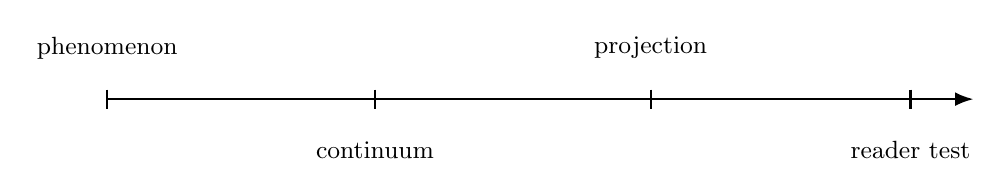
\begin{tikzpicture}[node distance=1.35cm,>=Latex,every node/.style={font=\small}]
\draw[->,thick] (0,0) -- (11,0);
\node[align=center] at (0,0.65) {phenomenon};
\node[align=center] at (3.4,-0.65) {continuum};
\node[align=center] at (6.9,0.65) {projection};
\node[align=center] at (10.2,-0.65) {reader test};
\foreach \x in {0,3.4,6.9,10.2} \draw[thick] (\x,0.12) -- (\x,-0.12);
\end{tikzpicture}
\caption{Axes Primitive Directions of: historical timeline of conceptual dependency pressure 31-1-26}
\label{fig:figure-axes-primitive-directions-of-resolution-one}
\end{figure}
The point of the diagram is not decoration; it marks which relation is being proposed and which stronger conclusion is still unavailable.\par
A local clarification is useful here\par
A local clarification is useful here\footnote{In Axes Primitive Directions of, this note clarifies the reader clarification role of the term and keeps the caveat close to the sentence that needs it.}.\par
The note keeps the caveat near the term without derailing the main sentence.\par
Those primitive directions are axes. An axis is not a line drawn on a graph after the real work is done. It is the direction along which a system can vary while still being treated as the same candidate system. In the clinic, time pressure is one such direction because many different states can be compared by the urgency under which decisions must be made. Clinical uncertainty is another because cases differ in how determinate the diagnosis is. Resource strain is another because the same medical problem changes when staff, rooms, oxygen, and attention become scarce. Institutional legitimacy is another because the clinic must act in ways that remain answerable to patients, law, and professional norms.\par
These directions do not prove anything about the clinic. They do something more modest and more necessary: they make explicit what kinds of difference later claims must respect. Without axes, the clinic appears as a heap of features: beds, nurses, protocols, oxygen, waiting times, symptoms, decisions, money, fatigue. With axes, those features begin to sort themselves according to the kinds of tension they can help resolve or intensify.\par
The starting point is practical. A clinician, administrator, patient, or analyst may notice different parts of the same strained situation. One sees a queue forming. Another sees diagnostic ambiguity. Another sees staff fatigue. Another sees a patient who no longer trusts the process. The axis vocabulary asks what direction of resolution each notice invokes when it becomes a claim. This does not make subjective impression final. It makes the first act of description accountable: before a system can be measured, modeled, or judged, one must say what sort of variation is being noticed.\par
\section{Axes Before Continua In Axes Primitive Directions of}
The distinction between an axis and a variable is easy to miss because mature sciences often encounter the world through already stabilized variables. Waiting time, number of clinicians on shift, room occupancy, oxygen saturation, and positive test rate can all be measured or assigned. They are variables inside chosen representations. An axis is more primitive. It gathers the direction of comparison that makes several variables jointly meaningful. \cite{klir_architecture_systems,maturana_varela_autopoiesis}\par
Waiting time, consultation length, arrival rate, and reporting delay may all participate in a time-pressure axis. Staff count, room turnover, supply restocking, and equipment availability may all participate in a resource-strain axis. Consent procedure, documentation quality, complaint frequency, and legal obligation may all participate in a legitimacy axis. The axis is not a hidden variable behind them. It is the direction under which they become relevant to the same problem of resolution.\par
The local dependency can now be written without changing the claim it supports.\par
\begin{equation}\label{eq:equation-axes-primitive-directions-of-resolution-two}
\operatorname{regularityResidual}_{7} = \tau_{\mathrm{repair}}=\inf\{t:C(t)<\theta\}
\end{equation}
The relation names a local dependency, variable dictionary, and proof/evidence role; it is not a claim-status upgrade.\par
The formula is a restraint on the prose. It names the dependency that the surrounding paragraph is allowed to use.\par
The comparison below gives axes primitive directions of a set of quantities that can be inspected instead of merely admired.\par
\begin{table}[htbp]
\centering\small
\caption{Axes Primitive Directions of: observable quantities and counter-pressure 31-2-26}
\label{tab:table-axes-primitive-directions-of-resolution-one}
\begin{tabular}{@{}llll@{}}
\toprule
Claim & Support carrier & Residual & Interpretation \\
\midrule
axes primitive directions of boundary & 87 units & declared case & fixes what is compared \\
residual pressure & 0.21 & dimensionless & shows unresolved load \\
projection loss & 0.58 & bounded interval & marks lost structure \\
countercase set & 34 cases & review sample & keeps a falsifier visible \\
\bottomrule
\end{tabular}
\end{table}
The table should be read locally: it narrows the comparison without pretending that the wider theory has been settled by a single surface.\par
This matters because systems often fail to fit a single observational style. A clinic is not exhausted by listing its parts, nor by measuring its outputs, nor by describing its official rules. It has material limits, procedural rhythms, clinical uncertainties, legal obligations, human bodies, and social expectations. George Klir's systems work is useful here because it reminds us that system description is organized rather than merely enumerative: objects, attributes, relations, and transformations matter together. The point is not to inherit a complete architecture from systems theory. The point is narrower: a system description must say how its elements are being organized before stronger claims can be trusted.\par
An axis therefore belongs to the beginning of analysis, but it is not beyond criticism. A proposed axis can be redundant if it only renames distinctions already carried by another axis. It can be too broad if it absorbs every tension and stops discriminating among cases. It can be too local if it applies only to one anecdote and cannot survive comparison across configurations. It can be empirically unsupported if the variables or observations invoked in its name do not actually move together in the relevant domain. Naming an axis is an invitation to scrutiny, not a license to decorate the system with impressive words.\par
The clinic gives a simple example. If one proposes an axis called administrative burden, the question is not whether administration exists. It plainly does. The question is what contrast the axis preserves. Does movement along it change possible resolutions? Does it remain intelligible across ordinary days, surge days, staffing shortages, audit events, and emergency improvisations? Does it differ from resource strain, legitimacy, or time pressure, or does it merely bundle pieces of them under a new label? If the proposed axis cannot answer these questions, it may still be a useful local observation, but it has not yet earned primitive status.\par
\section{Operators And Their Burden In Axes Primitive Directions of}
Axes become necessary because resolution is local before it is global. To resolve a tension is not to improve everything. It is to change a descriptive or operational state well enough for the system to continue under the description being used. Adding a temporary triage nurse may reduce the mismatch between arrival rate and decision capacity. It may not reduce diagnostic uncertainty, restore depleted supplies, or improve institutional trust. A resolution along one axis can leave another axis untouched or even make it worse. \cite{klir_architecture_systems,maturana_varela_autopoiesis}\par
This is one reason system language needs more discipline than ordinary talk about improvement. In institutional life, successful action is often reported as if success were global. The clinic reduced waiting time. The clinic increased throughput. The clinic protected staff. Each sentence may be true, yet each may hide the axis on which success was achieved. Shorter waits may come from shorter consultations. Higher throughput may come from weaker documentation. Staff protection may come from rejecting more borderline cases. A local resolution becomes misleading when it is narrated as a universal repair.\par
The local dependency can now be written without changing the claim it supports.\par
\begin{equation}\label{eq:equation-axes-primitive-directions-of-resolution-one}
\operatorname{complexityVerifier}_{7} = \operatorname{loss}_{\phi}=1-\frac{|E_{\phi}\cap E_{\mathrm{domain}}|}{|E_{\mathrm{domain}}|}
\end{equation}
The relation names a local dependency, variable dictionary, and proof/evidence role; it is not a claim-status upgrade.\par
The formula is a restraint on the prose. It names the dependency that the surrounding paragraph is allowed to use.\par
The local dependency can now be written without changing the claim it supports.\par
\begin{equation}\label{eq:equation-axes-primitive-directions-of-resolution-three}
\operatorname{rankGrowthToy}_{7} = I_{\mathrm{axis}}=\frac{\operatorname{Var}(x\mid a)}{\operatorname{Var}(x)}
\end{equation}
The relation names a local dependency, variable dictionary, and proof/evidence role; it is not a claim-status upgrade.\par
The formula is a restraint on the prose. It names the dependency that the surrounding paragraph is allowed to use.\par
A small numerical test keeps the abstraction honest at the scale of a single decision.\par
\paragraph{Numerical example.} For axes primitive directions of, take support=0.45, projection loss=0., and 6 open obligations. The bounded score is 0.; the example gives the reader a numeric scale without pretending to be empirical proof.\par
The numbers are deliberately small; their value is pedagogical, not evidential, unless the chapter binds them to a dataset elsewhere.\par
Configuration is the companion idea. A configuration is an arrangement of relations, states, and boundaries considered together. The clinic at 9 a.m. with three clinicians, twenty patients, normal supplies, and functioning referral pathways is one configuration. The clinic at 6 p.m. with two exhausted clinicians, no isolation rooms, delayed test results, and an ambulance diversion request is another. The clinic may remain recognizably the same clinic across both configurations, but the axes along which it is strained have changed in intensity and relation.\par
The ordering is not arbitrary. Axis comes first because we need directions of comparison. Resolution follows because those directions matter only when tensions can be answered or fail to be answered. Configuration follows because no axis operates alone in an actual system. Time pressure, uncertainty, resource strain, and legitimacy do not float separately above the clinic. They meet in arrangements of bodies, rooms, procedures, decisions, and responsibilities. A configuration is where the axes become entangled.\par
This modest vocabulary protects against two opposite errors. One error is to reduce the system to a list of variables and then wonder why the description has no grasp of institutional life. The other is to speak of the system as an indivisible whole and then lose the ability to say what changed. Axes, resolutions, and configurations occupy the middle ground. They let a description remain structured without pretending, too early, to be complete.\par
\section{A Claim Made Inspectable In Axes Primitive Directions of}
The clinic is useful because its tensions are familiar. But axes are not a convenience for healthcare analysis. The same need appears wherever a system can be described plausibly in more than one way and where those descriptions strain against one another. Consider a forest after several dry seasons. One description says the forest is a collection of species, soils, slopes, water flows, and weather patterns. Another says it is a carbon store. Another says it is habitat. Another says it is a fuel field. Another says it is a cultural and economic landscape. Each description can be valid, and none can safely absorb all the others. \cite{klir_architecture_systems,maturana_varela_autopoiesis}\par
Drought pressure is one axis because configurations can be compared by the degree to which water limitation reorganizes plant stress, soil moisture, and fire susceptibility. Biodiversity integrity is another because the forest can vary in the richness and resilience of its ecological relations. Fuel continuity is another because the spatial arrangement of dry matter changes how fire can spread. Human access and intervention form another because roads, crews, ownership, and policy alter what actions are possible. As in the clinic, these axes are not measurements by themselves. Rainfall, canopy moisture, species counts, deadwood volume, road density, and suppression capacity may become variables inside them. The axis is the direction of comparison that makes those variables matter together.\par
The case that follows turns the proposal into a sequence of criticizable moves.\par
\paragraph{Worked case.} In the worked case for axes primitive directions of, the claim is reduced to a boundary, an observable, a dependency, a numerical cue, and a falsifier. The case is useful only because each move can be criticized separately.\par
The case helps because each step can fail separately, which is exactly what a useful example should permit.\par
The forest example also shows why a single axis can mislead. If the system is described only through carbon storage, a dense plantation may look successful. If it is described only through fire suppression, aggressive clearing may look successful. If it is described only through biodiversity, certain interventions may appear destructive even when they reduce catastrophic fire risk. The relevant question is not which axis is morally superior in the abstract. It is what kind of resolution is being sought, what other axes it affects, and whether the configuration can remain viable under the resulting pressures.\par
A controlled burn, for instance, is an operator in this ecological setting. It transforms fuel continuity and may reduce future fire intensity. It can also affect habitat, air quality, public trust, and near-term carbon release. Its status cannot be read from one continuum alone. The same action may be protective under one axis, costly under another, and necessary only within a particular configuration of drought, vegetation, terrain, season, and institutional capacity. This is exactly the kind of situation in which axes matter: not because they make judgment easy, but because they prevent judgment from collapsing too soon into one preferred measure.\par
The second domain clarifies the generality of the concept. In the clinic, axes organize tensions among care, capacity, uncertainty, and legitimacy. In the forest, they organize tensions among water stress, ecological relation, fuel structure, and intervention. The domains differ, but the descriptive problem recurs. A system becomes intelligible only when one can say along which directions it is being strained and along which directions action might resolve, displace, or deepen that strain.\par
\section{What The Formula Does Not Prove In Axes Primitive Directions of}
An axis by itself names a direction. Once that direction is named, another question appears: what kinds of positions can a configuration occupy along it? A clinic is not simply under time pressure or not under time pressure. It may be moving from ordinary pacing to congestion, from congestion to overload, from overload to crisis triage, and from crisis triage to breakdown. A forest is not simply dry or wet. It may be passing through degrees of water stress that alter growth, disease vulnerability, ignition risk, and recovery capacity. The axis opens the direction; the continuum gives the field of possible comparison. \cite{klir_architecture_systems,maturana_varela_autopoiesis}\par
A continuum is a structured field of positions along one or more axes in which neighboring configurations can be compared without treating every difference as a total break. The word must be handled carefully. A continuum is not necessarily a smooth mathematical line. Some continua are measured discretely but operate continuously in practice. Staff count changes by whole persons, yet resource strain can intensify through fatigue, room turnover, delayed cleaning, supply restocking, and administrative delay. Species counts may be discrete, yet ecological integrity can erode through linked losses of pollination, shade, soil retention, and reproductive cycles.\par
Some continua also contain thresholds. A patient changes formally from waiting to admitted by decision, but the clinical condition leading to that decision may have been developing for hours. A forest may shift from recoverable drought stress to widespread mortality after interacting pressures cross a threshold. Continuum language keeps together gradual variation, comparability, and possible transition without assuming that every domain has the same mathematical texture.\par
This is a matter of scientific discipline. Calling something a continuum does not establish that it has been measured, modeled, simulated, or proven. It says only that a set of configurations is being treated as comparable along declared axes. If a later claim says the continuum has a metric, the metric must be supplied. If it says a transition occurs at a threshold, the threshold must be specified or the claim must remain qualitative. If it says the continuum appears in data, the data and method become part of the claim. The vocabulary makes stronger work possible; it does not smuggle that work in advance.\par
Murray Gell-Mann's notion of effective complexity helps by contrast. Effective complexity concerns the description of regularities in systems that are neither trivially ordered nor merely random. A continuum, as used here, is not the same thing. It is not a measure of descriptive richness. It is an organized space of comparison. A random jumble of clinic events would not yet be a continuum. A perfectly rigid script with no meaningful variation would not do the work either. A continuum appears where variation is organized enough to compare and open enough to require resolution.\par
In the clinic, a resource-strain continuum might move from reserve capacity through tight capacity, substitution, rationing, and exhaustion. A legitimacy continuum might move from routine accountability through exceptional justification, disputed authority, and loss of institutional trust. In the forest, a fuel-continuity continuum might move from patchy and interrupted fuel through connected understory, ladder fuels, crown continuity, and landscape-scale spread potential. These names are not measurements by themselves. They are disciplined positions in a descriptive field, awaiting whatever measurements, models, or case evidence the domain can responsibly provide.\par
\section{The First Formal Move In Axes Primitive Directions of axesS06}
The reason continua matter is not only that they arrange positions. It is that movement along one continuum can alter movement along another. High time pressure in the clinic may force substitutions that increase legitimacy risk. High uncertainty may consume resources, intensifying time pressure. Resource exhaustion may make documentation weaker, which may later damage trust. In the forest, drought pressure may increase fuel vulnerability; fuel continuity may change the consequences of human access; intervention may protect one ecological relation while disturbing another. \cite{klir_architecture_systems,maturana_varela_autopoiesis}\par
This is where the account leaves the territory of a set of checks. A set of checks can say that time, uncertainty, resources, and legitimacy all matter. It can say that drought, biodiversity, fuel, and intervention all matter. A continuum account says that each concern has a direction of variation, that configurations occupy positions along those directions, and that movement in one direction can change the available movements in another. The clinic is not merely a place with many concerns. It is a configuration moving through coupled continua. The forest is not merely a landscape with many values. It is a configuration in which ecological, material, climatic, and institutional pressures transform one another.\par
The practical consequence is sharp. If the clinic treats time pressure as the only serious continuum, then faster processing will appear rational even when it undermines diagnosis or legitimacy. If the forest treats fuel reduction as the only serious continuum, then intervention will appear rational even when it destroys ecological relations that support long-term resilience. Conversely, if legitimacy or biodiversity becomes the only continuum, necessary action may be paralyzed. Coupled continua make visible why local resolution must be judged by its transformations across the configuration.\par
This visibility is not a call for infinite complexity. A description that names too many axes becomes unusable. It loses the power to discriminate. The discipline lies in selecting axes that carry stable contrast, change possible resolution, and persist across configurations. A proposed axis must earn its place by helping explain what would otherwise be confused. When it stops doing that work, it should be revised, merged, demoted, or abandoned.\par
The strongest test is counterfactual. If removing a proposed axis changes nothing about the analysis, the axis is probably redundant. If every event can be placed on it with equal plausibility, it is probably too broad. If it matters only once and never again, it is probably a local feature. If it cannot be linked to observations, practices, variables, or consequences in the domain, it is probably unsupported. Axes are primitive, but they are not untouchable.\par
\section{Axes Before Continua In Axes Primitive Directions of axesS07}
Axes and continua describe possible variation, but they do not yet explain how a system moves, preserves itself, or fails. For that, the account needs operators. An operator is a rule, action, process, or transformation that changes a configuration or preserves it under changing conditions. The concept arrives here because the earlier concepts have reached their limit. A map of pressure does not say what moves. A field of possible positions does not say what transforms one position into another. \cite{klir_architecture_systems,maturana_varela_autopoiesis}\par
In the clinic, opening an overflow room is an operator on resource strain. Reassigning a clinician from follow-up visits to triage is an operator on time pressure and decision capacity. Requiring senior review before discharge is an operator on uncertainty and legitimacy. Diverting patients to another facility is an operator on local overload and regional coordination. Each action changes the configuration, but none changes it in only one way.\par
The operator vocabulary prevents a common mistake: treating a system's state as if it explained itself. A clinic under overload does not move toward recovery merely because overload has been named. Something must transform the configuration. The transformation may succeed, fail, or create another tension. Calling in extra staff may reduce waiting time while increasing fatigue later in the week. Relaxing documentation may improve speed while increasing accountability risk. Sending patients elsewhere may reduce local strain while worsening the burden on another institution.\par
Operators can also be non-intentional. Viral spread through a waiting room transforms a clinic configuration without being chosen by anyone. A software outage, a broken oxygen line, a rumor among patients, or a sudden weather event can operate on the clinic's continua. In the forest, lightning, insect infestation, invasive growth, windfall, and drought all operate on configurations without intention. Human decisions are only one class of transformation among others.\par
This broader view matters because the vocabulary must be able to speak across physical, biological, institutional, computational, and mixed systems without flattening their differences. In computation, a scheduler reallocating processing time is an operator on latency and throughput. A memory leak is a non-intentional operator on stability. A security patch may improve one continuum of vulnerability while disrupting another continuum of compatibility. The terms remain useful only if they do not pretend that all operators have the same kind of agency.\par
The value of axes becomes clearer once operators appear. If an axis is badly chosen, the operators attached to it will be misleading. Suppose the clinic is described only along efficiency. Then shortening consultations, reducing paperwork, and increasing turnover may all appear as improvements. But once uncertainty and legitimacy are visible, the same operations become more complex. A faster consultation may be an improvement under one continuum and a deterioration under another. The operator is not good or bad in the abstract. Its status depends on the axes and continua it transforms.\par
\section{Operators And Their Burden In Axes Primitive Directions of axesS08}
Some systems cannot be described adequately from outside alone. This claim requires care. In biology, Humberto Maturana and Francisco Varela introduced autopoiesis to describe living systems that produce and maintain their own organization. A clinic is not autopoietic in that biological sense. It does not produce itself as a living cell does. The analogy is partial and limited. Still, the biological discussion supplies an important caution: certain systems must be described partly through the way their organization is preserved while they interact with an environment. \cite{klir_architecture_systems,maturana_varela_autopoiesis}\par
The clinic does not merely receive patients and produce outputs. It preserves roles, procedures, records, responsibilities, and norms that allow its actions to count as clinical actions. Triage, consent, referral, and discharge are not only physical events. They are institutionally formed operations. A person leaving a room is not automatically a discharge. A conversation is not automatically informed consent. A priority decision is not automatically triage. These acts depend on an organization that gives them their meaning and force.\par
Varela's later work on autonomy sharpens the caution against treating systems as passive objects under external measurement. Used carefully, that caution helps explain why legitimacy is not an ornament added after medical facts. It is one of the directions along which the clinic remains a clinic. If procedures become arbitrary, records unreliable, consent meaningless, or accountability absent, then the organization that makes clinical action recognizable begins to fail. The claim is not that an institution is a living organism. The claim is that description must sometimes include the system's self-maintaining organization, not only the external inputs and outputs visible to an observer.\par
The forest example has a different structure. A forest is not an institution, but it too has forms of organization that matter to its persistence: soil relations, species dependencies, regeneration cycles, hydrological patterns, and disturbance regimes. A description that treats it only as standing timber or stored carbon may miss the relations that allow it to remain a forest across time. Here again, autonomy language must be used cautiously. The forest is not being granted a human-like purpose. The point is that organization can be part of what the system is, not merely a pattern projected onto it afterward.\par
Axis construction must therefore respect both external contrast and organized persistence. Time pressure can be counted in minutes, but its meaning changes with uncertainty and obligation. Resource strain can be counted in rooms and staff, but its meaning changes with the clinic's role in a regional health system. Drought can be measured through rainfall and moisture, but its ecological significance changes with species composition, soil condition, and fuel structure. A good axis keeps these differences available for later analysis instead of erasing them too early.\par
\section{A Claim Made Inspectable In Axes Primitive Directions of axesS09}
The boundary of the axis concept is plain. An axis is a primitive direction of resolution in a system description. It is not already a theorem, a measurement scale, a data column, a causal law, a simulation parameter, or a proof. Those stronger forms may appear later only when they are built. The axis prepares them by making the direction of comparison visible. It does not substitute for them. \cite{klir_architecture_systems,maturana_varela_autopoiesis}\par
This boundary is what keeps the account honest. When one says that a clinic moves along a time-pressure continuum, the statement may remain qualitative unless a measurement is supplied. When one says that legitimacy is an axis, one has not implied that legitimacy has a universal numerical scale. When one says that a forest is moving toward a fire-risk threshold, the threshold must either be specified by the relevant science and practice or acknowledged as a qualitative judgment. The language makes the claim articulable; it does not complete the investigation.\par
The same restraint applies to intellectual inheritance. Klir is useful because he clarifies that system description requires organized relations rather than mere listing. Maturana and Varela are useful because they show why self-maintaining organization complicates purely external description, though institutional analogies must remain limited. Gell-Mann is useful because organized complexity differs from both trivial order and undisciplined complication. These references do not compel the present account to be true. They help locate why the problem is real and why a lean vocabulary is needed.\par
The clinic can now be stated without flattening it. A clinic under respiratory surge is a configuration. Time pressure, clinical uncertainty, resource strain, and institutional legitimacy are candidate axes because they name primitive directions in which its tensions vary. The corresponding continua allow configurations to be compared across those directions. Operators such as triage reassignment, overflow rooms, senior review, diversion, and documentation changes transform positions within or across those continua. A boundary appears where the clinic can no longer preserve the organization that makes its operations count as clinic operations.\par
The forest can be stated in the same form without becoming the same case. A drought-stressed forest is a configuration. Water stress, biodiversity integrity, fuel continuity, and intervention capacity are candidate axes because they name directions in which its pressures vary. Continua allow comparison among ordinary dryness, stress, vulnerability, transition, and breakdown. Operators such as controlled burning, thinning, suppression, invasive spread, lightning, and seasonal rain transform those positions. The shared vocabulary does not erase the difference between medicine and ecology. It makes the difference describable without forcing both domains into one borrowed model.\par
\section{What The Formula Does Not Prove In Axes Primitive Directions of axesS10}
Axes matter because later thinking fails without them. One cannot speak responsibly about continua unless the direction of continuity has been named. One cannot speak clearly about boundaries unless the directions across which preservation and failure occur have been made explicit. One cannot judge operators without knowing which continua they transform. One cannot discuss contradiction, emergence, or collapse without first identifying the primitive directions along which resolution is sought and denied. \cite{klir_architecture_systems,maturana_varela_autopoiesis}\par
This is why axes must be primitive but not grandiose. They are early because they orient the description. They are modest because they do not by themselves guarantee measurement, causality, prediction, or proof. Their strength lies in making the first commitments visible. Once visible, those commitments can be narrowed, tested, formalized, revised, or rejected.\par
The mature use of an axis is neither decorative nor defensive. It lets a reader see what would otherwise remain confused: that a faster clinic may be a less reliable clinic, that a protected staff may mean a riskier waiting room, that a safer forest today may be a more fragile forest tomorrow, that one kind of resolution can become another kind of problem. A system is not clarified by pretending that all its tensions belong to one scale. It is clarified by finding the directions along which its tensions become answerable.\par
The chapter's argument therefore ends where later analysis must begin. Axes do not solve the system. They give the description its first disciplined orientation. They show where variation matters, where action can take hold, where local resolution may fail to become global repair, and where a configuration may cease to preserve the organization that made it recognizable. Before a theory can become formal, empirical, or operational, it must know in what directions its world can be resolved.\par
\chapter{Binary and Higher-Order Axes}
\section{The First Formal Move In Binary Higher-Order Axes}
A system first becomes visible when something no longer fits the description already being used. A room can be described by its temperature until two people in it begin arguing over whether it is comfortable. The thermometer has not failed. The original description has become too narrow. Comfort depends on bodies, clothing, movement, habit, expectation, and the purpose for which the room is being used. The trigger is not mystery for its own sake. It is the practical discovery that one line of measurement no longer carries the difference that matters. \cite{maturana_varela_autopoiesis,varela_biological_autonomy}\par
Organizational Continuum, abbreviated here as OC, begins from this kind of failure in description. OC calls this moment an encounter with an axis problem. An axis is a directed way of distinguishing one condition from another: hot and cold, open and closed, active and inactive, stable and unstable. A binary axis is the simplest case, because it begins with two poles. It does not mean that the world itself has only two values. It means that a system is being approached through a contrast sharp enough to organize observation.\par
The next diagram slows the argument down just enough to show how binary higher-order axes is being organized.\par
\begin{figure}[htbp]
\centering
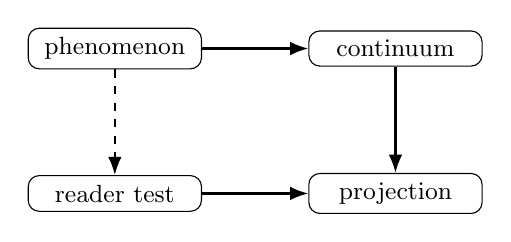
\begin{tikzpicture}[node distance=1.35cm,>=Latex,every node/.style={font=\small}]
\node[draw,rounded corners,align=center,minimum width=2.2cm] (a) {phenomenon};
\node[draw,rounded corners,align=center,minimum width=2.2cm,right=of a] (b) {continuum};
\node[draw,rounded corners,align=center,minimum width=2.2cm,below=of b] (c) {projection};
\node[draw,rounded corners,align=center,minimum width=2.2cm,left=of c] (d) {reader test};
\draw[->,thick] (a) -- (b);
\draw[->,thick] (b) -- (c);
\draw[->,thick] (d) -- (c);
\draw[->,thick,dashed] (a) -- (d);
\end{tikzpicture}
\caption{Binary Higher-Order Axes: dependency dag of conceptual dependency pressure 32-1-27}
\label{fig:figure-binary-and-higher-order-axes-one}
\end{figure}
The point of the diagram is not decoration; it marks which relation is being proposed and which stronger conclusion is still unavailable.\par
A local clarification is useful here\par
A local clarification is useful here\footnote{In Binary Higher-Order Axes, this note clarifies the reader clarification role of the term and keeps the caveat close to the sentence that needs it.}.\par
The note keeps the caveat near the term without derailing the main sentence.\par
The biological background matters because living systems are not merely objects with properties. Maturana and Varela described living organization through autopoiesis: a living system continually produces and maintains the network that makes it the kind of system it is. This helps OC see why a boundary is not just an outline drawn around a thing. A boundary participates in the conditions under which a system remains describable as itself.\par
The first lesson is modest. Binary language is useful when it exposes a real distinction in the situation. It becomes dangerous when the distinction is mistaken for the whole situation. OC begins with binary axes because they are the smallest operational handles on difference, not because all continua are secretly binary.\par
\section{Axes Before Continua In Binary Higher-Order Axes}
The primitive term in this chapter is not object but distinction. A distinction is a repeatable separation between conditions. When a switch is off rather than on, when a membrane admits one molecule and excludes another, when a social role permits one action and forbids another, a distinction is doing work. The term is intentionally spare. It does not require the same instruments, scales, or causes in every domain. \cite{maturana_varela_autopoiesis,varela_biological_autonomy}\par
An axis is a stabilized distinction. It has at least two poles, and it allows observations to be placed with respect to those poles. In ordinary speech, left and right form an axis; so do permitted and forbidden, awake and asleep, compressed and expanded. In OC, the axis is not just a label. It is the rule by which a difference becomes available for comparison.\par
The local dependency can now be written without changing the claim it supports.\par
\begin{equation}\label{eq:equation-binary-and-higher-order-axes-two}
\operatorname{institutionalLatency}_{7} = \rho_{\mathrm{replay}}=\frac{N_{\mathrm{matched}}}{N_{\mathrm{declared}}}
\end{equation}
The relation names a local dependency, variable dictionary, and proof/evidence role; it is not a claim-status upgrade.\par
The formula is a restraint on the prose. It names the dependency that the surrounding paragraph is allowed to use.\par
The comparison below gives binary higher-order axes a set of quantities that can be inspected instead of merely admired.\par
\begin{table}[htbp]
\centering\small
\caption{Binary Higher-Order Axes: observable quantities and counter-pressure 32-2-27}
\label{tab:table-binary-and-higher-order-axes-one}
\begin{tabular}{@{}llll@{}}
\toprule
Model & Retained insight & Rejected assumption & OC extension \\
\midrule
binary higher-order axes boundary & 90 units & declared case & fixes what is compared \\
residual pressure & 0.28 & dimensionless & shows unresolved load \\
projection loss & 0.69 & bounded interval & marks lost structure \\
countercase set & 35 cases & review sample & keeps a falsifier visible \\
\bottomrule
\end{tabular}
\end{table}
The table should be read locally: it narrows the comparison without pretending that the wider theory has been settled by a single surface.\par
A state is a position with respect to one or more axes. A boundary is a condition that separates admissible from inadmissible movement across states. A continuum is the ordered field of possible positions generated when an axis or family of axes supports more than one describable condition. These definitions are operational. They tell the reader what role the terms play before any stronger mathematical or scientific claim is attempted.\par
The word operator enters later, but its need can already be felt. A system does not merely sit on axes. It changes, resists change, converts one kind of difference into another, and sometimes fails to preserve itself under transformation. Before the term can bear weight, the simpler vocabulary has to be stable enough to say what is being transformed.\par
\section{Operators And Their Burden In Binary Higher-Order Axes}
An axis is constructed when a distinction becomes disciplined enough to be reused. Consider a cell membrane. One description treats the membrane as inside versus outside. That is a binary axis. It is crude, but it is not empty. It allows the cell to be discussed as a bounded organization rather than a diffuse chemical cloud. Varela's work on biological autonomy sharpens the point: autonomy is not isolation, but organized self-production and regulation within a surrounding world. \cite{maturana_varela_autopoiesis,varela_biological_autonomy}\par
The inside-outside axis immediately raises a difficulty. Some molecules pass through the membrane, some are blocked, and some pass only under specific conditions. The original binary distinction still matters, but it no longer contains enough detail. The description now needs permeability, selectivity, energy cost, timing, and context. A higher order axis appears when the first distinction forces further distinctions that cannot be reduced back to the original pair without losing the phenomenon.\par
The local dependency can now be written without changing the claim it supports.\par
\begin{equation}\label{eq:equation-binary-and-higher-order-axes-one}
\operatorname{socialCoordination}_{7} = G=(V_{\mathrm{claim}}\cup V_{\mathrm{evidence}},E_{\mathrm{support}}\cup E_{\mathrm{challenge}})
\end{equation}
The relation names a local dependency, variable dictionary, and proof/evidence role; it is not a claim-status upgrade.\par
The formula is a restraint on the prose. It names the dependency that the surrounding paragraph is allowed to use.\par
The local dependency can now be written without changing the claim it supports.\par
\begin{equation}\label{eq:equation-binary-and-higher-order-axes-three}
\operatorname{biologicalRobustness}_{7} = \epsilon_{\mathrm{domain}}=\max_i |y_i-\hat y_i|
\end{equation}
The relation names a local dependency, variable dictionary, and proof/evidence role; it is not a claim-status upgrade.\par
The formula is a restraint on the prose. It names the dependency that the surrounding paragraph is allowed to use.\par
A small numerical test keeps the abstraction honest at the scale of a single decision.\par
\paragraph{Numerical example.} For binary higher-order axes, take support=0.48, projection loss=0.12, and 1 open obligations. The bounded score is 0.180; the example gives the reader a numeric scale without pretending to be empirical proof.\par
The numbers are deliberately small; their value is pedagogical, not evidential, unless the chapter binds them to a dataset elsewhere.\par
This is the basic movement of the chapter. A binary axis gives the first cut. A higher order axis appears when the cut remains useful but insufficient. The new axis does not erase the old one. It repositions it. Inside and outside still matter, but they are now embedded in a richer field: regulated exchange, boundary maintenance, and system continuity.\par
The same pattern appears in institutional life. A legal category such as lawful versus unlawful may begin as a binary axis. A person breaks a window in a locked building. If the act is described only as damage to property, it seems to fall cleanly on one side. But the case changes if the person saw smoke, heard a child inside, called emergency services, broke the smallest pane available, and waited for responders. The first distinction remains present, yet judgment now turns on intent, harm, exception, necessity, and remedy. The binary has been placed inside a more articulated continuum of judgment.\par
OC uses examples of this kind cautiously. A membrane and a court do not share the same materials, causes, or standards of evidence. They can still exhibit a comparable movement from first distinction to structured field. What matters is not a forced analogy between biology and law, but the recurring pressure exerted by insufficient distinctions.\par
\section{A Claim Made Inspectable In Binary Higher-Order Axes}
A continuum, in OC usage, is not merely a smooth line. It is a structured space of possible positions generated by one or more axes. Some continua may be close to numerical measurement, as with temperature or pressure. Others may be ordered without being easily measured, as with degrees of institutional authority or levels of biological autonomy. The central requirement is not smoothness. It is that positions can be distinguished, related, and transformed without pretending that all differences are of the same kind. \cite{maturana_varela_autopoiesis,varela_biological_autonomy}\par
This definition matters because the word continuum often suggests that every position between two poles must already be known. OC uses the term more cautiously. A continuum may contain gaps in measurement, uncertain regions, or domain-specific constraints. The point is that a field of possible positions has become available for disciplined description. The continuum is not a promise of complete knowledge.\par
The case that follows turns the proposal into a sequence of criticizable moves.\par
\paragraph{Worked case.} In the worked case for binary higher-order axes, the claim is reduced to a boundary, an observable, a dependency, a numerical cue, and a falsifier. The case is useful only because each move can be criticized separately.\par
The case helps because each step can fail separately, which is exactly what a useful example should permit.\par
Gell-Mann's account of effective complexity is relevant by contrast. Effective complexity concerns the structure of a description that captures regularities without merely listing randomness. For OC, this helps identify the pressure between compression and differentiation. Too little structure gives a heap of observations. Too much compression erases the differences that made the system worth studying.\par
Bialek's work on predictability and complexity adds another caution. A useful description of a system is often tied to what can be predicted, at what scale, and with what loss. OC's continua are not automatically predictive models. They are preparatory structures that make later predictive or explanatory claims more exact. If a later claim says that a contradiction generates a new dimension of description or collapses a configuration, the reader must first know what kind of space the contradiction is occurring in.\par
\section{What The Formula Does Not Prove In Binary Higher-Order Axes}
Axes and continua describe structured possibility, but systems are not exhausted by possible positions. They move. They regulate. They undergo transitions. They resist some transitions and permit others. A map of possible states is not yet an account of passage among them. \cite{maturana_varela_autopoiesis,varela_biological_autonomy}\par
Return to the room. Temperature is one axis. Comfort is another. Occupancy, airflow, clothing, and expectation introduce further axes. Someone opens a window. The air cools, but the change is not simply a move from warm toward cold. The room becomes noisier. A draft reaches one chair before another. The person near the window feels relief; the person across the room feels exposed; the argument shifts from comfort to consideration. One gesture has rearranged several relations at once.\par
Only after seeing that transformation does the need for a separate term become clear. An operator is a rule or process by which states are carried, constrained, or reconfigured across a continuum. In a biological example, metabolism transforms available chemical differences into maintained organization. In an institutional example, a rule transforms permitted action into recognized authority or sanctioned violation. These examples do not establish a single law of all systems. They show why transformation must be named separately from position.\par
The objection is immediate: does this vocabulary simply rename ordinary causation? It can overlap with causal language, but it asks a different question. Causation often asks what produced an event. An operator asks how a describable state-space is traversed or reorganized. The same physical cause may have different operator roles depending on the continuum being described. Heat may damage a cell, cook food, trigger an alarm, or change a legal classification of risk. OC keeps the operator tied to the description in which it functions.\par
\section{The First Formal Move In Binary Higher-Order Axes axesS06}
The vocabulary developed here has a narrow job. It prepares the terms needed for later claims. Binary axes, higher order axes, continua, boundaries, states, and operators are introduced as disciplined ways of speaking about difference and transformation. Their value depends on whether they let a claim be stated more clearly, tested more sharply, or rejected more cleanly in the domain where it is applied. \cite{maturana_varela_autopoiesis,varela_biological_autonomy}\par
The restraint matters. A binary axis can clarify a phenomenon, but it can also flatten it. A higher order axis can recover lost structure, but it can also multiply distinctions without improving understanding. A continuum can organize positions, but it can also suggest false smoothness. An operator can express transformation, but it can also conceal ambiguity behind a technical word. OC is useful only where its distinctions make a real burden of description easier to carry.\par
Maturana and Varela help OC recognize living boundaries as active conditions of organization. Gell-Mann helps frame the tension between compressed description and meaningful structure. Bialek helps keep description tied to scale, prediction, and loss. None of these sources transfers authority to OC by association. They mark neighboring problems that any serious language of systems must be able to face.\par
The chapter began with a room that was easy to measure and hard to settle. It moved to membranes, institutions, continua, and transformations because the same lesson keeps returning: the first distinction is often necessary, and rarely enough. A system becomes more visible as its axes become more precise, but precision is not the same as excess. The task is to find the distinctions that carry the phenomenon without burying it.\par
OC therefore begins with binary axes and refuses to end there. The binary gives the first hold on difference. Higher order axes show where that first hold must be refined. Continua give the refinement a field. Operators name the transformations that move through that field. With these pieces in place, the next question can be asked more cleanly: what happens when several axes interact, when boundaries constrain their movement, and when a system meets a contradiction it cannot resolve within its current descriptive space?\par
\chapter{Defining a Continuum}
\section{The First Formal Move In Defining Continuum}
A shoreline looks easy to name until one tries to say exactly where it is. At high tide, water covers stones that were dry in the morning. A wave runs up the sand, withdraws, and leaves a darker band behind it. A storm moves the visible edge inland. A harbor wall fixes one segment sharply, while a marsh lets water, mud, reeds, salt, and animal movement interpenetrate. The ordinary word shoreline still works, but it hides several distinct acts of description: where one stands, how long one watches, what scale one accepts, and what kind of change one is willing to treat as part of the same thing. \cite{varela_biological_autonomy,gell_mann_effective_complexity}\par
The first lesson is not that the shoreline is vague and therefore unusable. It is that a system can be stable enough to discuss while refusing to be captured by a single static edge. The shore does not vanish because the water moves. It also does not become a perfectly fixed object because a mapmaker draws a line. It is recognizable through variation, and that recognition depends on a disciplined tolerance: this much movement still belongs to the shore; this other movement belongs to another question.\par
The next diagram slows the argument down just enough to show how defining continuum is being organized.\par
\begin{figure}[htbp]
\centering
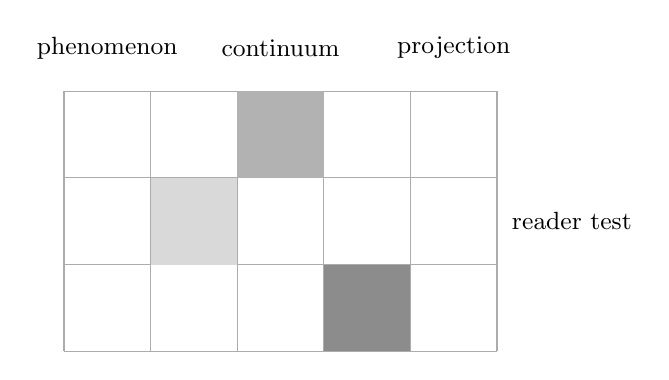
\begin{tikzpicture}[node distance=1.35cm,>=Latex,every node/.style={font=\small}]
\draw[step=1.1cm,gray!65,thin] (0,0) grid (5.5,3.3);
\node[align=center] at (0.55,3.85) {phenomenon};
\node[align=center] at (2.75,3.85) {continuum};
\node[align=center] at (4.95,3.85) {projection};
\node[align=center] at (6.45,1.65) {reader test};
\fill[black!15] (1.1,1.1) rectangle (2.2,2.2);
\fill[black!30] (2.2,2.2) rectangle (3.3,3.3);
\fill[black!45] (3.3,0) rectangle (4.4,1.1);
\end{tikzpicture}
\caption{Defining Continuum: evidence matrix of conceptual dependency pressure 33-1-28}
\label{fig:figure-defining-a-continuum-one}
\end{figure}
The point of the diagram is not decoration; it marks which relation is being proposed and which stronger conclusion is still unavailable.\par
A local clarification is useful here\par
A local clarification is useful here\footnote{In Defining Continuum, this note clarifies the reader clarification role of the term and keeps the caveat close to the sentence that needs it.}.\par
The note keeps the caveat near the term without derailing the main sentence.\par
OC calls this kind of ordered variability a continuum. A continuum is not simply a blur, a range, or a polite way of avoiding precision. It is a domain in which different positions or states can be compared because some relation among them remains stable. The stones exposed at low tide, the wet sand, the reeds at the marsh edge, the concrete harbor wall, and the seasonal drift of sediment do not all mean the same thing. Yet they can be studied together when the question is how land and sea meet across time, material, depth, salinity, use, and force.\par
The word earns its place because the ordinary scene already contains the problem. If one is navigating a boat, the relevant shore is partly a matter of depth and hazard. If one is settling a property dispute, the relevant shore may be a legally fixed line. If one is studying a salt marsh, the relevant shore includes water movement through soil, root systems, bird nesting, and nutrient exchange. If one is modeling climate exposure, the relevant shore includes storm surge and projected sea-level rise. These are not four opinions about a single obvious edge. They are four disciplined ways of making the shore comparable.\par
A continuum therefore begins from a practical need: to describe persistence through change without flattening change into sameness or dissolving persistence into noise. The shore remains itself only if the description is allowed to follow its movement. But the description remains useful only if it refuses to follow everything. The tides matter. The moon matters indirectly. The mineral structure of each grain of sand may matter for some question, but not for all. The habits of a person walking there at dawn may matter for public access, but not for erosion modeling. Every usable description keeps some relations in view and leaves others outside.\par
The same difficulty appears wherever organization survives disturbance. A living body, for example, does not persist by keeping all of its parts unchanged. Skin cells are shed and replaced. Heat rises and falls. A cut opens the surface, clots, inflames, seals, and remodels. The wound does not prove that the organism has ceased to be itself. On the contrary, the repair makes visible the kind of continuity involved. The body maintains identity through controlled variation: blood flow changes, immune cells gather, tissue regrows, and the boundary between body and world is restored in stages.\par
Francisco Varela's account of biological autonomy matters here because he treated living organization not as a thing merely enclosed by a border, but as an activity that continually produces and maintains its own identity. The membrane, the metabolism, and the organism's relation to its surroundings are not separate ornaments added to a preexisting object. They are part of the living pattern itself. A bacterium regulating exchange through its membrane, or an animal closing a wound, shows why a fixed boundary is not enough. The boundary must be understood as something made, maintained, repaired, and sometimes redrawn by the system's own activity.\par
The shoreline and the wound are different scenes, but they teach the same caution. A stable word may point to a changing organization. The task is not to deny the change, and not to surrender the word. The task is to say what variation belongs to the description, how the variation can be compared, and where the comparison stops.\par
\section{Axes Before Continua In Defining Continuum}
A continuum is an ordered domain of possible variation within which states, positions, or descriptions remain comparable under a stated rule of relevance. That sentence is compact, but each part comes from an ordinary act already visible at the shore. There must be variation, because a single frozen point gives nothing to compare. There must be order, because scattered differences do not yet form a usable domain. There must be relevance, because no description can include every possible fact. There must be a limit, because comparison without an edge expands until it loses meaning. \cite{varela_biological_autonomy,gell_mann_effective_complexity}\par
Variation is the easiest part to see. The shore changes with tide, weather, season, construction, erosion, plant growth, and animal movement. A body changes with hunger, heat, injury, fatigue, infection, and repair. An institution changes with leadership, money, law, communication, habit, and public trust. If nothing can differ, there is no continuum, only repetition. But variation alone is not enough. A drawer full of unrelated objects varies. A rumor mutating randomly through a crowd varies. A sequence of disconnected labels varies. None of these becomes a continuum until a comparison can be made.\par
The local dependency can now be written without changing the claim it supports.\par
\begin{equation}\label{eq:equation-defining-a-continuum-two}
\operatorname{physicalContinuity}_{7} = \kappa_{K_7}=\frac{b_{K_7}+s_{K_7}}{1+o_{K_7}+q_{K_7}}
\end{equation}
The relation names a local dependency, variable dictionary, and proof/evidence role; it is not a claim-status upgrade.\par
The formula is a restraint on the prose. It names the dependency that the surrounding paragraph is allowed to use.\par
The comparison below gives defining continuum a set of quantities that can be inspected instead of merely admired.\par
\begin{table}[htbp]
\centering\small
\caption{Defining Continuum: observable quantities and counter-pressure 33-2-28}
\label{tab:table-defining-a-continuum-one}
\begin{tabular}{@{}llll@{}}
\toprule
Input & Operation & Output & Open condition \\
\midrule
defining continuum boundary & 93 units & declared case & fixes what is compared \\
residual pressure & 0.35 & dimensionless & shows unresolved load \\
projection loss & 0.80 & bounded interval & marks lost structure \\
countercase set & 36 cases & review sample & keeps a falsifier visible \\
\bottomrule
\end{tabular}
\end{table}
The table should be read locally: it narrows the comparison without pretending that the wider theory has been settled by a single surface.\par
Order is the difference between mere difference and intelligible difference. The order need not be a neat straight line. The waterline rises and falls, but the marsh also changes by saturation, salinity, root density, sediment, and species movement. Wound repair passes through phases, but those phases overlap: clotting, inflammation, tissue growth, and remodeling do not behave like beads on a string. A city agency may become more centralized in budget while remaining decentralized in local judgment. These are still ordered domains if the differences can be tracked in a disciplined way.\par
Murray Gell-Mann's work on complexity is useful at this point because it emphasizes that a good description is neither a complete listing of every microscopic detail nor a crude slogan. The important description captures regularities that matter while leaving out noise that would bury the pattern. A tide chart does not list every molecule of water. A medical account of healing does not track every atom in a scab. Yet each can be more informative than an exhaustive record because it selects structure at the right level.\par
Relevance is what keeps selection honest. To say that the shore has moved is not yet complete. Moved for whom, and for what purpose? The navigator, ecologist, property lawyer, insurer, and local resident may each need a different account. The differences are not arbitrary just because they depend on the question. Navigation is constrained by depth and hazard. Ecology is constrained by organism exchange and habitat. Law is constrained by recognized procedures and enforceable marks. Climate planning is constrained by probable future exposure. The same place can therefore support several continua, each legitimate when its relevance is named.\par
This is where many descriptions become careless. A word such as boundary, integration, complexity, centralization, or autonomy is often carried from one question to another as if its meaning survives unchanged. Sometimes it does. Often it does not. The boundary of a marsh for a botanist may not be the boundary of a parcel for a court. The boundary of a body for an immune response may not be the boundary assumed by a photograph. A continuum does not solve this problem automatically, but it forces the writer or analyst to make the comparison visible.\par
A limit is not a failure of understanding. It is a condition of understanding. The shoreline continuum may include tide, sediment, vegetation, and storm history while excluding the quantum state of each molecule. The exclusion is not denial. It is a statement that the description is operating at a certain scale for a certain question. A physician treating a wound may need circulation, infection, tissue depth, pain, and immune response. She does not need the full biography of the patient for every clinical judgment, though that biography may matter in another setting. The limit makes attention possible.\par
This gives the term continuum a narrower and stronger meaning than common usage often suggests. It is not a decorative word for complexity. It is not any smooth scale between two extremes. It is not a way to dignify uncertainty. It is a bounded domain of relevant variation in which comparison remains possible. A shore can be mapped, walked, defended, restored, litigated, and inhabited because different continuities can be drawn from the same changing place. The discipline lies in saying which continuity is being used.\par
\section{Operators And Their Burden In Defining Continuum}
Consider a social institution that is said to be becoming more centralized. The statement sounds clear until a concrete case is put under it. Imagine a public health agency responding to outbreaks across a large region. Before a crisis, local clinics decide staffing, purchase ordinary supplies, report cases through a shared database, and follow broad national rules. During the crisis, the central office begins issuing daily instructions, controlling vaccine distribution, approving public messages, and setting thresholds for school closures. Everyone may agree that centralization has increased, but the agreement may hide several different movements. \cite{varela_biological_autonomy,gell_mann_effective_complexity}\par
Command authority is one movement. If local directors once decided when to open weekend clinics and now must wait for central approval, authority has shifted. Budget control is another. If money still sits in local accounts but can be spent only under central categories, the institution has centralized financially even if local managers still sign the invoices. Communications routing is another. If information from clinics once moved horizontally among neighboring districts but now must pass through a central dashboard before anyone can act on it, the communication structure has changed. Legal enforcement is another still. If the central office can issue binding orders rather than recommendations, the institution has changed its power, not merely its coordination.\par
The local dependency can now be written without changing the claim it supports.\par
\begin{equation}\label{eq:equation-defining-a-continuum-one}
\operatorname{chemicalPathway}_{7} = \operatorname{support}(c_{7})=P(c_{7})\wedge E(c_{7})\wedge R(c_{7})
\end{equation}
The relation names a local dependency, variable dictionary, and proof/evidence role; it is not a claim-status upgrade.\par
The formula is a restraint on the prose. It names the dependency that the surrounding paragraph is allowed to use.\par
The local dependency can now be written without changing the claim it supports.\par
\begin{equation}\label{eq:equation-defining-a-continuum-three}
\operatorname{cognitiveLoad}_{7} = \operatorname{falsify}(h)=\exists e\in E\,:\,\operatorname{pred}_h(e)\neq\operatorname{obs}(e)
\end{equation}
The relation names a local dependency, variable dictionary, and proof/evidence role; it is not a claim-status upgrade.\par
The formula is a restraint on the prose. It names the dependency that the surrounding paragraph is allowed to use.\par
A small numerical test keeps the abstraction honest at the scale of a single decision.\par
\paragraph{Numerical example.} For defining continuum, take support=0.51, projection loss=0.17, and 2 open obligations. The bounded score is 0.113; the example gives the reader a numeric scale without pretending to be empirical proof.\par
The numbers are deliberately small; their value is pedagogical, not evidential, unless the chapter binds them to a dataset elsewhere.\par
These movements can align, but they need not. A central office may control public messaging while leaving medical judgment local. It may centralize purchasing while decentralizing outreach. It may gather all data centrally while allowing local experimentation. A single sentence about centralization therefore becomes analytically weak unless the relevant continuum is named. Are we comparing command, money, information, law, symbolic legitimacy, or operational dependence? Each produces a different ordering of the same institution.\par
The payoff is not pedantry. It changes what one can see. Suppose the agency fails in one district. A loose description might say the failure came from too much centralization. But if command remained local, budgets were central, communication was delayed, and legal authority was ambiguous, the problem may lie in a mismatch among continua. Local clinics may have been blamed for choices they no longer had the resources to make. The central office may have received data too slowly to coordinate supply. Public messages may have appeared unified while operational responsibility remained fragmented. Without the continuum, the analysis collapses distinct failures into one political label.\par
The shoreline helps again. A seawall centralizes one kind of boundary. It gives a hard line where waves meet concrete. But it does not centralize the whole coastal system. Water still moves through drainage, sand still shifts at the wall's base, pressure gathers at weak points, and habitats may reorganize around the interruption. To call the shore fixed because one segment has been hardened is to mistake one continuum for all of them. The wall fixes a legal and engineering edge more than it fixes the movement of the sea.\par
A cognitive example shows the same pattern at a smaller scale. Think of remembering a melody. The memory is not stored or recalled as a row of identical units. One person may remember the contour but not the key. Another remembers rhythm but not words. A musician may transpose the melody and still recognize it. A child may hum the final phrase and lose the beginning. The melody persists through changes in pitch, tempo, instrument, timbre, and accuracy because some relations remain comparable. But again the relevant continuum must be named. Are we studying acoustic frequency, motor habit, emotional association, cultural recognition, or neural prediction?\par
William Bialek's work on prediction and complexity is relevant here because it links structure to what observations allow one to anticipate. A sequence is not meaningful merely because it contains many bits of difference. It becomes structured when past and present observations constrain what may come next. In a melody, the listener's expectation is part of the order. In a coastline, tidal records let one anticipate water movement. In an institution, reporting patterns allow people to anticipate decisions. A continuum is useful because it makes such comparison possible without requiring all details to be identical.\par
The biological case can be made just as concrete. A small cut on a hand breaks the surface that usually separates tissue from the world. For a few moments, blood flows outward. Then clotting begins. The area warms and swells as immune activity changes local conditions. New tissue forms. The scab dries. Later, the scar fades or remains. At no point is the organism simply identical to its prior state, yet the process is not random. The body is moving through a repair continuum in which boundary condition, immune response, tissue integrity, pain, and function change together in ordered but uneven ways.\par
If one described the body only by the visible edge of the skin, the wound would appear as a temporary failure of boundary. If one described it only by immune activation, the same wound would appear as a regulated defensive process. If one described it by mobility, the relevant question might be whether the hand can still grip. If one described it by infection risk, the important boundary might be microbial rather than visual. The organism has not become many unrelated things. Rather, different continua become salient under different questions. Varela's point about autonomy clarifies why: the living system is maintaining itself through activity, not merely sitting behind a line.\par
Giulio Tononi's theory of integrated information belongs nearby, but carefully. Its contribution is not that every use of the word integration has been settled. It gives one formal way to ask how a whole may generate information beyond independently considered parts. That is a precise family of questions, especially in debates about consciousness. It does not license a general habit of calling any connected system integrated in the same sense. A wound, a melody, a public agency, and a conscious experience may all involve relations among parts, but the relevant continua differ.\par
\section{A Claim Made Inspectable In Defining Continuum}
The temptation is to treat a boundary as the opposite of a continuum. If a thing has a boundary, one imagines it must be fixed. If it is continuous, one imagines it must have no edge. The shore shows why both images fail. The shoreline can be bounded for a map and still move with the tide. The marsh can be continuous in ecological exchange and still have limits for a study. The harbor wall can make one edge sharp while leaving the wider coastal system dynamic. A boundary does not destroy a continuum. It makes the continuum usable. \cite{varela_biological_autonomy,gell_mann_effective_complexity}\par
Every serious description therefore makes choices. Some choices are explicit, as when a survey defines the shore by the mean high-water mark. Some are hidden, as when a photograph taken at low tide is treated as if it shows the permanent edge. Some are practical, as when emergency planners choose the zone likely to flood under a particular storm model. Some are inherited from institutions, instruments, or habits of speech. OC uses the word projection for this act of selecting a relevant view from a richer situation, but the ordinary idea is simple: no description takes in everything, and the chosen angle matters.\par
The case that follows turns the proposal into a sequence of criticizable moves.\par
\paragraph{Worked case.} In the worked case for defining continuum, the claim is reduced to a boundary, an observable, a dependency, a numerical cue, and a falsifier. The case is useful only because each move can be criticized separately.\par
The case helps because each step can fail separately, which is exactly what a useful example should permit.\par
Projection in this sense is not fantasy. It is not the invention of a private world. A nautical chart, a habitat survey, and a legal map can all be constrained by evidence and still disagree because they select different relations. The disagreement is not automatically a contradiction. It becomes a contradiction only if the descriptions are forced to answer the same question in the same respect and cannot both hold. Until then, their difference may show that the underlying situation supports more than one valid continuum.\par
This distinction is essential for avoiding false arguments. One person says the shore is retreating because erosion has moved the dune line inland. Another says the legal shoreline has not moved because the recognized boundary remains fixed in public records. A third says the marsh is expanding because brackish vegetation has colonized new ground. The speakers may appear to disagree, but they may be tracking geomorphology, law, and ecology respectively. Their claims should not be merged until the continuum of comparison is clear.\par
The same happens in institutional life. A mayor announces that the public health agency has decentralized because neighborhood clinics can design their own outreach. A critic replies that it has centralized because all funding must now be approved by the central office. Both may be right. Outreach design and budget control are different continuities of organization. The political argument becomes confused if decentralization is treated as a single substance that must increase or decrease everywhere at once.\par
Once the relevant continuum is named, finer tools become possible. One can ask along which dimension the change occurred. A dimension of comparison within a continuum can be called an axis: command authority, budget control, communication routing, or legal enforcement in the institutional example; salinity, depth, vegetation, or tidal reach at the shore; inflammation, tissue closure, pain, or function in wound repair. The word axis should not make the idea seem more technical than it is. It names the respect in which comparison is being made.\par
One can also ask what changes a position within the continuum. A storm moves the shoreline in one way, a seawall in another, and a new legal survey in another. A clot changes the wound's condition. A budget rule changes an agency's centralization. A repeated melody changes a listener's expectation. OC calls such change-making acts operators when they are treated formally: transformations that move, stabilize, connect, separate, intensify, or interrupt positions within a continuum. The ordinary point comes first. Something happens, and the relevant state changes in a describable way.\par
This is why a continuum is prior to stronger claims about emergence, collapse, or hierarchy. Before saying that a new form has emerged, one must know the domain in which novelty is being judged. Before saying that a structure has collapsed, one must know which relations had previously held together. Before arranging levels into a hierarchy, one must know what varies within each level and what comparison links one level to another. Otherwise the language outruns the case.\par
\section{What The Formula Does Not Prove In Defining Continuum}
The absence of a continuum does not merely make prose untidy. It produces false clarity. A concept appears sharp because it has been reduced too quickly. The shore becomes a line. The organism becomes a container. The institution becomes centralized or decentralized. The melody becomes the notes on a page. Each reduction may be useful in a narrow context, but each becomes misleading when it is mistaken for the whole organized situation. \cite{varela_biological_autonomy,gell_mann_effective_complexity}\par
Return to the public health agency. If centralization is treated as one scale, the agency can be ranked from local to central and the analysis can proceed quickly. But the speed is purchased by blindness. Suppose the central office controls funds and legal orders, local clinics control clinical judgment, communications are routed through a slow central database, and public trust depends on neighborhood relationships. During an outbreak, a delay in vaccine delivery may be blamed on local inefficiency. Yet the relevant continuum may be budget control. A confusing public message may be blamed on central command. Yet the relevant continuum may be trust and communication routing. The wrong continuum leads to the wrong remedy.\par
The biological case is equally unforgiving. If a wound is described only as a break in the body's boundary, then inflammation can look like additional disorder: redness, swelling, heat, pain. But within the repair continuum, these changes may be signs of organized response. If inflammation continues too long, however, the same signs may indicate pathology. The meaning of the state depends on where it sits in the ordered process of repair and which comparison is being made. Without that continuum, the description cannot distinguish repair from damage with enough precision.\par
The cognitive case has its own version. A person who remembers a melody in the wrong key has not simply failed to remember it. If the relevant continuum is exact pitch, the memory is wrong. If the relevant continuum is melodic contour, the memory may be intact. If the relevant continuum is emotional association, the altered performance may preserve what matters most to the listener. The question is not whether anything goes. The question is what kind of sameness is at stake.\par
These examples also show why neighboring terms cannot replace the continuum. A spectrum is often a single ordering from less to more. Some continua contain such orderings, but many require several dimensions at once. A process is change through time, but a continuum can compare possible states even before a particular system moves through them. A category says what belongs; a continuum asks how differences within or across belonging are organized. A field distributes values across positions; some continua behave that way, while others depend more on function, relation, or rule. A hierarchy orders levels; a continuum explains what variation is being compared within or across those levels.\par
The distinctions matter only because they prevent mistakes. A marsh is not just a point on a wet-to-dry spectrum, because salinity, vegetation, sediment, animal use, and tidal flow do not reduce cleanly to one line. Wound repair is not just a process, because the same temporal sequence must be interpreted through boundary integrity, immune regulation, tissue function, and systemic health. A public agency is not just a hierarchy, because formal rank may diverge from money, information, and trust. A remembered melody is not just a category, because recognition may survive across transformations.\par
The cautions can be stated tightly. A continuum is not proof that a claim is true. It is the descriptive surface on which a claim can be made without equivocation. A continuum is not ambiguity. It requires an ordering rule. A continuum is not necessarily smooth. Many organized domains are uneven, branching, interrupted, or multidimensional. A continuum is not a decorative synonym for complexity. It must say what varies, how comparison is ordered, why the comparison is relevant, and where the description stops.\par
These limits protect scientific status rather than weakening it. OC does not become stronger by borrowing the prestige of adjacent theories. Varela helps clarify self-maintaining organization in living systems. Gell-Mann helps clarify why useful descriptions compress regularity rather than list everything. Bialek helps connect structure with prediction from observation. Tononi helps show how integration can be made into a formal question about wholes and parts. None of these contributions proves OC. They mark difficulties any serious account of organized variation must face.\par
\section{The First Formal Move In Defining Continuum definiti}
Once a continuum has been defined, a claim can no longer pretend to have unlimited reach. It must answer modest but demanding questions. What is varying? In what respect are the variations comparable? What rule makes some differences relevant and others secondary? Where does the description stop? What changes the state of the system, and what merely changes the observer's view? These questions do not settle the inquiry, but they keep it from beginning in confusion. \cite{varela_biological_autonomy,gell_mann_effective_complexity}\par
At the shore, the same storm may operate differently across several continua. It can move sand, kill vegetation, breach a dune, alter salinity, damage buildings, and change insurance maps. One event does not have one meaning. Its meaning depends on the organized domain under consideration. If the question is ecological recovery, the relevant state may involve root systems and species return. If the question is navigation, it may involve depth and obstruction. If the question is law, it may involve recognized boundaries and liability. The storm is real in all cases. The continuum determines what kind of change is being named.\par
In the body, an infection can also move through several continua. It may increase immune activity, reduce tissue integrity, alter temperature, limit function, and change the relation between organism and environment. A fever is not simply more heat. It belongs to a regulated response, unless it exceeds the range in which regulation remains viable. A scar is not simply less injury. It may restore closure while altering sensation or movement. Continuity is not the absence of transformation. It is the preservation of comparability through transformation.\par
In social life, reform often fails because it changes one continuum while claiming victory in another. A government may decentralize service delivery while centralizing measurement. A company may flatten job titles while concentrating budget approval. A university may grant departments curricular freedom while tightening control over hiring. These arrangements are not inherently incoherent. They become incoherent when public language treats them as one movement. The continuum reveals whether a reform is mixed, aligned, symbolic, operational, or contradictory.\par
Contradiction becomes more precise under this discipline. If two descriptions conflict, the conflict may mean that one is false. It may also mean that they operate on different continua, that the boundary of comparison has been drawn badly, that an important dimension has been omitted, or that the system is undergoing a change not captured by the inherited description. A shoreline that is legally fixed and physically retreating is not automatically a logical puzzle. It becomes a practical and conceptual problem when law, risk, ownership, and ecological change must be made to answer together.\par
This is the point at which stronger OC terms become necessary, but they should arise from the pressure of examples rather than from terminology alone. An axis names a dimension of comparison. An operator names a transformation that changes position or relation within the continuum. A projection names the selected view under which the richer situation becomes describable. Emergence names the appearance of a new organized pattern that cannot be captured by the old comparison alone. Collapse names a loss of organization within a previously usable comparison. Hierarchy names an ordering among levels, but only after the continua within those levels have been made visible.\par
The terms do not add seriousness by themselves. They are useful only when they return to the cases. In the shoreline case, a new inlet after a storm may not be merely a shifted line; it may create a new circulation pattern, alter habitats, and change human access. In the wound case, infection may transform repair into systemic risk. In the institutional case, a central data platform may create a new form of authority even if formal law remains unchanged. In the melody case, a variation may become a new theme rather than an error. Each claim depends on the continuum against which change is judged.\par
The discipline is therefore both restrictive and enabling. It restricts loose language by requiring named comparison. It enables richer language because, once the comparison is clear, one can describe transformation without reducing it to a slogan. A continuum is the minimal object needed before a theory of organized change can speak responsibly.\par
\section{Axes Before Continua In Defining Continuum definiti}
A continuum is a bounded, ordered domain of relevant variation. It allows a system, pattern, or description to remain comparable without remaining identical. The term is useful because many of the most important objects of inquiry are neither fixed things nor formless flows. They persist by changing, and they change in ways that can be ordered if the right comparison is chosen. \cite{varela_biological_autonomy,gell_mann_effective_complexity}\par
The shoreline remains recognizable while moving. Its edge can be walked, mapped, defended, restored, and disputed, but no single edge exhausts it. A living organism maintains itself through exchange, repair, and regulation, not by freezing its material state. A public institution can centralize money, decentralize judgment, route communication through one hub, and disperse trust across neighborhoods. A melody can survive transposition and fail under exact repetition if the relevant relation has been lost. These are not exceptions to clarity. They are the cases clarity must learn to handle.\par
The boundary is not an embarrassment. It is what lets the continuum do work. Without a boundary, the description expands until it includes everything. Without variation, it has nothing to compare. Without order, it has only difference. Without relevance, it cannot explain why this comparison matters rather than another. A continuum holds these requirements together.\par
The unresolved case is now visible. After a storm, a coastal town finds that its legal shoreline, ecological shoreline, navigational shoreline, and lived shoreline no longer meet. The map still names one boundary. The marsh has moved. The channel has shifted. Houses that were safe by the old measure now flood. Residents still speak of the same place, but the former description no longer carries all the relations that matter. The problem is not simply that the shore changed. The problem is that several continua have been forced into contact, and their mismatch now demands a new act of description.\par
\chapter{Support, Boundary, and Threshold}
\section{The First Formal Move In Support Boundary Threshold}
A system is not understood merely because something has been named inside it. A storm, a cell, a market, a household, and a political institution can all be described as systems, but the word does little work until the description says what is being held together, what can change without destroying the case, and what would count as a different case. The local problem is therefore not whether the world contains wholes. It plainly does. The problem is how to speak about a whole without smuggling in more unity, stability, or evidence than the observation permits. \cite{gell_mann_effective_complexity,bialek_predictability_complexity}\par
This problem appears whenever inquiry needs a unit. The unit may be obvious in ordinary speech and unstable under analysis. A lake has a name, a basin, a shoreline, a history of use, and a place on a map. Those facts make it easy to treat the lake as a ready-made object. Yet the same lake can be picked out by several different operations. It can be measured as a hydrological body, owned as a parcel or collection of parcels, regulated as a public resource, remembered as a local place, modeled as an ecological regime, or sampled as a microbial habitat. The word lake remains useful, but it does not by itself determine which object of inquiry is being used.\par
The next diagram slows the argument down just enough to show how support boundary threshold is being organized.\par
\begin{figure}[htbp]
\centering
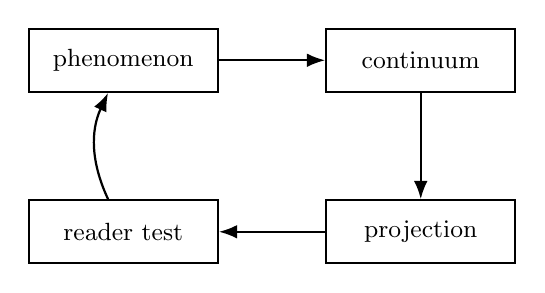
\begin{tikzpicture}[node distance=1.35cm,>=Latex,every node/.style={font=\small}]
\node[draw,thick,align=center,minimum width=2.4cm,minimum height=0.8cm] (a) {phenomenon};
\node[draw,thick,align=center,minimum width=2.4cm,minimum height=0.8cm,right=of a] (b) {continuum};
\node[draw,thick,align=center,minimum width=2.4cm,minimum height=0.8cm,below=of b] (c) {projection};
\node[draw,thick,align=center,minimum width=2.4cm,minimum height=0.8cm,left=of c] (d) {reader test};
\draw[->,thick] (a) -- (b);
\draw[->,thick] (b) -- (c);
\draw[->,thick] (c) -- (d);
\draw[->,thick,bend left=25] (d) to (a);
\end{tikzpicture}
\caption{Support Boundary Threshold: phase diagram of conceptual dependency pressure 34-1-29}
\label{fig:figure-support-boundary-and-threshold-one}
\end{figure}
The point of the diagram is not decoration; it marks which relation is being proposed and which stronger conclusion is still unavailable.\par
A local clarification is useful here\par
A local clarification is useful here\footnote{In Support Boundary Threshold, this note clarifies the reader clarification role of the term and keeps the caveat close to the sentence that needs it.}.\par
The note keeps the caveat near the term without derailing the main sentence.\par
An object, in this vocabulary, is a stabilized unit of description. It is not first a thing with an eternal essence, nor is it merely a word imposed on passive matter. It is a case held steady enough that operations can be applied, comparisons can be made, and differences can be judged. The lake is one object for an inquiry tracking nutrient load and water clarity. It is another object for an inquiry tracking legal ownership, another for recreation, another for flood control, and another for microbial ecology. This does not make the lake imaginary. It means that objecthood, for inquiry, depends on how the case is picked out, held apart from neighboring cases, and followed through change.\par
Consider a lake approaching a regime shift. For years it may look like the same lake: same basin, same name on the map, same shoreline in ordinary weather. People may fish from the same dock and point to the same water from the same road. Yet phosphorus load, algal density, oxygen distribution, plant cover, and feedback between turbidity and vegetation may be moving the lake toward a different operating condition. Scheffer's work on critical transitions made this kind of case vivid: gradual pressure can bring a system near a threshold after which the visible state changes abruptly (scheffer critical transitions). The lake example gives the three words of this chapter their first operational use. Support names what presently holds a description in place. Boundary names the limit across which the description no longer applies unchanged. Threshold names a boundary condition at which small additional change can alter the system's operating regime.\par
\section{Axes Before Continua In Support Boundary Threshold}
To call the lake an object is to say that a description has enough stability to be used. It is not to say that all possible descriptions of the lake collapse into one. A summer visitor, a limnologist, an insurer, a town planner, and a farmer upstream may all speak about the same lake while relying on different boundaries and different tests of sameness. The visitor may notice color, odor, swimming conditions, and the presence of fish. The limnologist may track chlorophyll, phosphorus, dissolved oxygen, macrophyte cover, and turbidity. The insurer may attend to flood levels and shoreline risk. The farmer may think first of drainage, runoff, and permitted use. These descriptions overlap, but they are not interchangeable. \cite{gell_mann_effective_complexity,bialek_predictability_complexity}\par
An operator is a repeatable way of changing or reading an object. Adding phosphorus is an operator on the lake's chemical and ecological state. Measuring chlorophyll is an operator of observation. Dredging sediment, changing inflow, introducing a fish species, drawing a legal boundary, issuing a permit, or installing a monitoring station are all operators in different registers. Some operators affect the lake materially. Others affect access, classification, obligation, or evidence. The distinction matters because support, boundary, and threshold are not decorative labels attached after description. They are discovered by asking what operations preserve the object, what operations deform it, and what operations make the old description fail.\par
The local dependency can now be written without changing the claim it supports.\par
\begin{equation}\label{eq:equation-support-boundary-and-threshold-two}
\operatorname{technologyCoupling}_{8} = C_{\mathrm{unres}}=\min_{\pi\in\Pi}\|B(x)-B(\pi x)\|
\end{equation}
The relation names a local dependency, variable dictionary, and proof/evidence role; it is not a claim-status upgrade.\par
The formula is a restraint on the prose. It names the dependency that the surrounding paragraph is allowed to use.\par
The comparison below gives support boundary threshold a set of quantities that can be inspected instead of merely admired.\par
\begin{table}[htbp]
\centering\small
\caption{Support Boundary Threshold: observable quantities and counter-pressure 34-2-29}
\label{tab:table-support-boundary-and-threshold-one}
\begin{tabular}{@{}llll@{}}
\toprule
Case step & Observable & Numerical cue & Caveat \\
\midrule
support boundary threshold boundary & 9 units & declared case & fixes what is compared \\
residual pressure & 0.21 & dimensionless & shows unresolved load \\
projection loss & 0.33 & bounded interval & marks lost structure \\
countercase set & 8 cases & review sample & keeps a falsifier visible \\
\bottomrule
\end{tabular}
\end{table}
The table should be read locally: it narrows the comparison without pretending that the wider theory has been settled by a single surface.\par
The same physical situation can therefore contain several objects of inquiry at once. A legal object may persist while an ecological object has changed. A parcel boundary may remain stable in the registry while the water chemistry has crossed into a new regime. Conversely, a legal reclassification may occur while the lake's ecological state remains continuous. The framework does not ask the reader to choose one of these as the real lake and dismiss the others as mere perspectives. It asks for discipline about which object is being discussed, which operators matter, and which tests would show that the description has stopped carrying.\par
This discipline is needed because ordinary language hides changes in objecthood. We often continue to use the same noun after the operative case has changed. A forest after fire, a currency after hyperinflation, a constitution after capture, a body after sepsis, and a lake after eutrophication may all keep their names while ceasing to support some of the descriptions formerly attached to them. The name supplies continuity in speech. Inquiry has to decide whether that continuity is supported by the variables, operations, and comparisons that the claim requires.\par
\section{Operators And Their Burden In Support Boundary Threshold}
Return to the lake before drawing any general rule from it. The first question is not where its edge lies, but what makes the current description hold. If the inquiry concerns a clear-water ecological state, support may be found in submerged plants, low turbidity, balanced nutrient cycling, oxygen distribution, grazing pressure, and feedbacks that keep algae from dominating. Seasonal variation does not by itself destroy support. A storm may muddy the water for a few days. A hot month may change oxygen levels. A spring pulse may carry nutrients from fields into the basin. The description remains supported if those changes fall within a range that the same account can absorb. \cite{gell_mann_effective_complexity,bialek_predictability_complexity}\par
Support is the present adequacy of a description under permitted operations. It is not psychological confidence, and it is not mere repetition of a name. A description has support when the relations it depends on continue to organize the case across relevant variation. If water clarity changes seasonally but the same ecological account still predicts, classifies, and explains the observations, the description has support across that seasonal range. If a disturbance changes the dominant feedbacks so that the former account no longer predicts or classifies the case well, the earlier support has weakened or ended. Support is therefore relational. It belongs neither to the observer alone nor to the object alone, but to the fit between a stabilized object, chosen features, and tested operations.\par
The local dependency can now be written without changing the claim it supports.\par
\begin{equation}\label{eq:equation-support-boundary-and-threshold-one}
\operatorname{agencyChoice}_{8} = \Delta d=\operatorname{rank}(A_{\mathrm{new}})-\operatorname{rank}(A_{\mathrm{old}})
\end{equation}
The relation names a local dependency, variable dictionary, and proof/evidence role; it is not a claim-status upgrade.\par
The formula is a restraint on the prose. It names the dependency that the surrounding paragraph is allowed to use.\par
The local dependency can now be written without changing the claim it supports.\par
\begin{equation}\label{eq:equation-support-boundary-and-threshold-three}
\operatorname{aiAlignmentProxy}_{8} = P_{\mathrm{collapse}}=\sigma(\alpha R-\beta S-\gamma M)
\end{equation}
The relation names a local dependency, variable dictionary, and proof/evidence role; it is not a claim-status upgrade.\par
The formula is a restraint on the prose. It names the dependency that the surrounding paragraph is allowed to use.\par
A small numerical test keeps the abstraction honest at the scale of a single decision.\par
\paragraph{Numerical example.} For support boundary threshold, take support=0.54, projection loss=0.10, and 3 open obligations. The bounded score is 0.110; the example gives the reader a numeric scale without pretending to be empirical proof.\par
The numbers are deliberately small; their value is pedagogical, not evidential, unless the chapter binds them to a dataset elsewhere.\par
Boundary is derived from this loss of carryover. A boundary is not merely an edge in space. It is the limit of valid transfer for a description. The shoreline is a spatial boundary for some purposes, but the ecological boundary of the lake may include inflowing streams, runoff from fields, groundwater exchange, or atmospheric deposition. The administrative boundary may exclude all of those. A recreational boundary may follow access points, docks, beaches, and boat launches. A microbial boundary may vary with temperature layers, sediment, and oxygen gradients. The operational question is always the same: across what change does the same description still carry, and across what change does it need replacement or translation into another vocabulary?\par
A concrete mismatch makes the point clearer. Suppose a county draws a property boundary around the parcels touching the lake and assigns responsibility for shoreline management to those owners. The line may be clear in law. It may determine tax, liability, fencing, access, and repair obligations. Yet the watershed that feeds the lake may extend far beyond those parcels. Fertilizer applied several miles away, drainage changes upstream, and road runoff from outside the lakeside properties may carry phosphorus into the basin. If the legal boundary is mistaken for the ecological boundary, the resulting policy will look orderly while failing causally. It will regulate the people nearest the water while leaving some of the strongest operators outside the frame. The legal object and the ecological object overlap, but their boundaries do not coincide.\par
This does not mean that the legal boundary is false or useless. It is valid for the operations it supports: ownership, permitted entry, liability, taxation, and administrative jurisdiction. It fails only when carried without translation into a claim about nutrient flow or regime stability. The error lies in boundary transfer. A line that works for one object is treated as if it automatically works for another. The same error appears when an electoral district is taken as a cultural community, when a firm's accounting boundary is treated as the boundary of its environmental impact, or when a diagnostic category is treated as the full boundary of a lived condition. In each case the question is not whether the boundary exists. It is whether the boundary supports the claim being made.\par
Threshold is a special kind of boundary. It is not any limit whatever, but a limit at which the relation between additional change and system response becomes discontinuous, highly nonlinear, or newly organized. The lake may tolerate nutrient increases for a time while remaining recognizably in a clear-water state. Then a further increase, perhaps small relative to the total loading history, can help shift the dominant feedbacks. Turbidity rises, plant cover collapses, algae dominate, and the old description no longer organizes the case. The threshold is not simply the moment when the lake looks unpleasant. It is the condition at which the operating relations that supported the former object have changed.\par
A threshold may be visible only after careful reconstruction. In the lake case, the water may not announce in advance that it is near a regime change. Early warning indicators may be partial, noisy, or absent. Historical data may be thin. Several variables may move at once. The concept therefore carries scientific discipline only when it is tied to observable indicators, explicit variables, and a stated uncertainty about whether the proposed threshold has actually been reached. Threshold language is powerful because some systems really do change by regime. It is dangerous because many changes merely become dramatic in retrospect.\par
\section{A Claim Made Inspectable In Support Boundary Threshold}
The terms can be stated without equations, but they are prepared for later formal use by keeping their roles separate. Support is the present adequacy of a description under permitted operations. Boundary is the limit of that adequacy. Threshold is a boundary condition associated with a change in regime, classification, or explanatory requirement. These definitions are intentionally modest. They do not assert that every system has a clean threshold, that every boundary is measurable in one metric, or that every support relation can be reduced to a single number. \cite{gell_mann_effective_complexity,bialek_predictability_complexity}\par
The modesty matters. A vocabulary that begins with system, object, support, boundary, and threshold can easily become grander than its evidence. The safer route is to let the terms mark positions in an argument rather than conclusions. A support claim says, in effect, that some description continues to hold under specified variation. A boundary claim says where that holding ceases. A threshold claim says that the cessation is not merely a gradual weakening but a change in operating regime, classification, or explanatory demand. Each claim invites tests. Each can be wrong.\par
The case that follows turns the proposal into a sequence of criticizable moves.\par
\paragraph{Worked case.} In the worked case for support boundary threshold, the claim is reduced to a boundary, an observable, a dependency, a numerical cue, and a falsifier. The case is useful only because each move can be criticized separately.\par
The case helps because each step can fail separately, which is exactly what a useful example should permit.\par
This is why the terms should be kept distinct even when they are empirically connected. A system can have support without a known threshold. A boundary can be useful without being sharp. A threshold can be suspected without being measured. A description can fail for reasons that are not threshold-like at all: missing variables, bad sampling, category error, scale mismatch, or imported assumptions from another domain. If these differences are blurred, the vocabulary stops helping inquiry and begins to protect vague claims from criticism.\par
The same separation also makes formalization possible without forcing premature mathematics. In some cases support may later be represented by stability under transformations, predictive adequacy, persistence of correlations, conservation of identity conditions, or resilience within a state space. Boundary may be represented by domain limits, classification surfaces, discontinuities, loss of invariance, jurisdictional edges, or failure of model transfer. Threshold may be represented by bifurcation, tipping point, phase transition, legal trigger, metabolic limit, institutional rupture, or decision point. These are not the same structure in every domain. The shared vocabulary is useful only if it keeps the differences visible.\par
This modesty aligns the vocabulary with several existing scientific intuitions without collapsing them into one theory. Gell-Mann's effective complexity concerns regularities that make a system describable without treating pure randomness as deep structure (gell mann effective complexity). Bialek's work on predictability and complexity connects structure to what can be learned from the past about the future (bialek predictability complexity). Tononi's information integration program asks when a system's state has a kind of irreducible unity relative to its parts (tononi information integration). The comparison is limited but useful: each case asks how organization can be real enough to support explanation without being mistaken for total unity, final proof, or a universal metric.\par
OC does not borrow these results as proof of its own claims. It takes from the comparison a disciplined concern with describable organization, predictive carryover, and unity under constraint; it refuses to infer that one measure of complexity, predictability, or integration can settle every question about objects, boundaries, and thresholds. The neighboring references show that the difficulty is not invented by vocabulary. It recurs wherever inquiry tries to distinguish mere aggregation from organized form, and organized form from the overstatement of form.\par
\section{What The Formula Does Not Prove In Support Boundary Threshold}
The main danger is verbal inflation. Once support, boundary, and threshold are available, it becomes tempting to apply them everywhere. A political movement has a boundary. A metabolic process has support. A market crosses a threshold. A legal order loses support. An ecosystem approaches a boundary. These sentences may be true, but none is scientific or even especially clear merely because it uses the vocabulary. Each must identify the object, the variables or features in view, the operations being applied, and the observations that distinguish ordinary variation from failure of the description. \cite{gell_mann_effective_complexity,bialek_predictability_complexity}\par
A political movement, for example, may be treated as an object only after the inquiry says what holds it together. Is the object a voting bloc, a party organization, a donor network, a shared ideology, a protest coalition, or a media identity? Each has different support. A party may lose ideological coherence while retaining ballot access and funding. A protest coalition may lose street presence while its language enters institutions. A donor network may persist after the public label fades. To say that the movement crossed a threshold is empty unless the claim identifies which object changed and what relation between additional pressure and response became discontinuous or newly organized.\par
A market example has the same burden. A price movement is not automatically a threshold. A firm can lose revenue gradually, then suddenly lose credit access because a covenant is breached. In that case the threshold may be legal-financial rather than psychological or purely economic. Before the covenant is breached, each additional loss may worsen the firm's condition without changing its operating classification. After the breach, lenders may accelerate obligations, suppliers may shorten terms, and buyers may doubt continuity. The same revenue decline now acts through a different structure. A threshold claim becomes plausible because a specified boundary condition changes the operations that can be applied to the firm.\par
A metabolic example requires equal care. The body may maintain blood glucose within a functional range through insulin response, glycogen storage, appetite, activity, and hormonal regulation. Support is not the mere fact that a number is normal at one moment. It is the stability of a regulatory relation under ordinary variation. A boundary may appear when the same regulatory description no longer carries, because the response is impaired or overwhelmed. A threshold claim would require more than saying that the body is under stress. It would need to identify a condition at which the operating regime changes, such as compensation giving way to decompensation, or a reversible imbalance becoming a crisis under defined clinical variables.\par
These examples show why the vocabulary is portable only under discipline. It can travel across ecology, law, politics, markets, metabolism, and thermodynamics because many inquiries face the same structural questions: what holds, where does it stop holding, and when does stopping become a change of regime? But portability is not permission to erase domain differences. The operators differ. The evidence differs. The consequences of error differ. A boundary in law may be enacted by text and authority. A boundary in ecology may be inferred from flows and feedbacks. A boundary in thermodynamics may be expressed through state variables. A boundary in politics may be contested by the very actors it describes.\par
An objection naturally follows: if objects depend on description, does the framework make reality dependent on language? No. The dependence runs through access and comparison, not through existence. The lake may change whether or not anyone names it correctly. A firm may default whether or not analysts use the right vocabulary. A body may enter crisis whether or not a clinician describes the transition elegantly. But inquiry can only compare states by selecting features and operations. The vocabulary makes that selection explicit so that claims can be narrowed, tested, or rejected.\par
A bad support claim can be defeated by showing that the alleged stabilizing relations do not hold. A bad boundary claim can be defeated by showing that the description carries farther than asserted, or fails earlier. A bad threshold claim can be defeated by showing that the supposed transition is gradual, mismeasured, reversible within the same regime, or unsupported by the chosen variables. The framework does not protect claims from defeat. It gives defeat clearer handles.\par
\section{The First Formal Move In Support Boundary Threshold threshol}
The vocabulary fails when it outruns its warrant. It fails if support becomes a synonym for confidence, if boundary becomes a metaphor for importance, or if threshold becomes a dramatic name for any change. It fails when an object is named but not stabilized, when an operator is implied but not stated, or when a domain is borrowed because its language sounds more rigorous than the evidence can bear. It also fails when continuity of name is mistaken for continuity of operating structure. \cite{gell_mann_effective_complexity,bialek_predictability_complexity}\par
It fails especially when domains are mixed without translation. A legal boundary cannot automatically serve as an ecological boundary. The lakeside property line may decide who can build a dock, but it does not decide where phosphorus enters the water. A thermodynamic threshold cannot automatically serve as a social threshold. A social threshold cannot automatically serve as a biological one. Projection between domains may be possible, and sometimes it is necessary, but it must be stated as projection. The loss, mismatch, and change of operator have to remain visible.\par
This failure boundary is not a weakness of the vocabulary. It is the condition that keeps the vocabulary useful. A concept that can go anywhere without changing has usually stopped saying much. Support, boundary, and threshold remain valuable only when they force the inquiry back to the object in question. What is being held together here? Which operations preserve it, disturb it, or reveal it? Where does the description stop carrying? Is the stopping gradual loss, category error, scale mismatch, or a genuine change of regime?\par
The consequence is simple but demanding. The three terms do not prove a theory, and they do not confer seriousness on a claim by their presence. They discipline attention. They require a description to show how its object is supported, where its boundary of carryover lies, and whether any proposed threshold is more than an after-the-fact name for surprise. Used this way, the terms prepare the ground on which evidence, formalization, and projection between domains can be inspected without confusing a name for an argument.\par
\chapter{Why Operators Are Needed}
\section{The First Formal Move In Operators Are Needed}
At rush hour, a city intersection is not difficult because cars exist. It is difficult because the same patch of asphalt must serve several purposes at once. A driver sees a route home. A pedestrian sees a place to cross. A traffic engineer sees timed movement through a network. An ambulance crew sees a delay that may cost minutes the patient does not have. The intersection remains one physical site, but it cannot be understood by listing its parts. Its difficulty lies in the way possible actions compete, constrain one another, and sometimes require the whole arrangement to be temporarily reorganized. \cite{bialek_predictability_complexity,tononi_information_integration}\par
This is where the need for operators begins. In ordinary language, an operator is something that makes a permitted change possible: a switch, a rule, a protocol, a calculation, a procedure, or a mechanism. The word will become more exact as the chapter proceeds, but its first sense is simple. If a system can be in one condition and then another, we need to say not only what changed, but what made the change legitimate, possible, or effective. At the intersection, the ambulance does not pass safely merely because it needs to pass. Something must reorder the situation.\par
The next diagram slows the argument down just enough to show how operators are needed is being organized.\par
\begin{figure}[htbp]
\centering
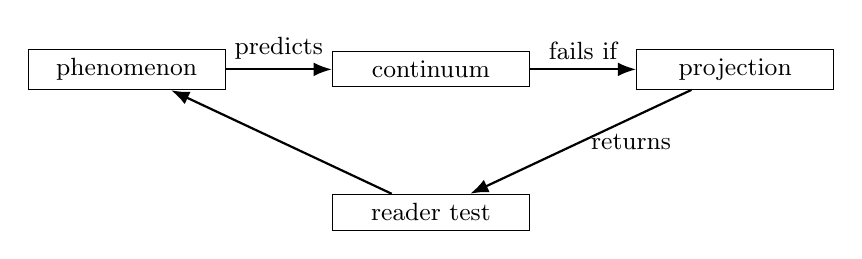
\begin{tikzpicture}[node distance=1.35cm,>=Latex,every node/.style={font=\small}]
\node[draw,align=center,minimum width=2.5cm] (c) {phenomenon};
\node[draw,align=center,minimum width=2.5cm,right=of c] (t) {continuum};
\node[draw,align=center,minimum width=2.5cm,right=of t] (f) {projection};
\node[draw,align=center,minimum width=2.5cm,below=of t] (r) {reader test};
\draw[->,thick] (c) -- node[above]{predicts} (t);
\draw[->,thick] (t) -- node[above]{fails if} (f);
\draw[->,thick] (f) -- node[right]{returns} (r);
\draw[->,thick] (r) -- (c);
\end{tikzpicture}
\caption{Operators Are Needed: falsifier of conceptual dependency pressure 35-1-30}
\label{fig:figure-why-operators-are-needed-one}
\end{figure}
The point of the diagram is not decoration; it marks which relation is being proposed and which stronger conclusion is still unavailable.\par
A local clarification is useful here\par
A local clarification is useful here\footnote{In Operators Are Needed, this note clarifies the reader clarification role of the term and keeps the caveat close to the sentence that needs it.}.\par
The note keeps the caveat near the term without derailing the main sentence.\par
Imagine the traffic lights continuing as usual while the ambulance approaches. North-south traffic has a green light. Pedestrians have already stepped into the crosswalk. East-west cars are stopped. The ambulance is coming from the west. If every participant follows the ordinary rule, the ambulance waits. If every participant improvises, the crossing becomes dangerous. The city therefore relies on a special form of action: an emergency priority protocol. It may turn some lights red, hold others, signal drivers to yield, and suspend ordinary timing for a short interval. That protocol is not another vehicle in the intersection. It is the organized transformation by which the intersection changes from ordinary flow to emergency passage.\par
Several features are already visible. The protocol acts on a described situation: the current signal pattern, the location of vehicles, the presence of pedestrians, and the approach of the ambulance. It acts only under conditions: an emergency vehicle must be detected or authorized, the equipment must function, and the law must require compliance. It produces a result: the intersection is temporarily reordered so that one kind of movement takes priority over others. If those conditions are absent, the protocol cannot do its work. A broken signal, a driver who refuses to yield, or a missing detection system may leave the ambulance facing the same physical road but a different practical world.\par
Many systems that matter have this form. They are not merely collections of objects. They are arrangements in which possible actions determine what can happen next. A locked door, a market price, a biological membrane, a software permission, a legal threshold, and a social norm all separate one condition from another. None is only a line. Each makes some transitions available, delays others, forbids others, and sometimes creates a new situation when ordinary alternatives fail. The operator names the form of action that carries such a transition when the transition is allowed.\par
The point is not to treat every domain as if it were traffic engineering. The point is to notice a recurring need in description. When water boils, a cell differentiates, a crowd panics, a model generalizes, or an institution adapts, a verb compresses the change. The sentence names a before and an after, but it may hide the structure that made the after reachable from the before. A serious account of change has to unpack that compression. It must ask what condition the system was in, what kind of action could act there, what limits governed the action, and what was changed by its success or failure.\par
Scientific work on complex systems gives this pressure a practical setting without settling the theory in advance. William Bialek's work on prediction and complexity, for example, asks how a system can contain structure that matters for future behavior even when that structure is not obvious from an inventory of parts. Giulio Tononi's work on integrated information is concerned with how parts of a system jointly constrain possible states rather than merely adding up as isolated pieces. Marten Scheffer and others have shown how some ecological systems can absorb pressure for a time and then shift rapidly into a different regime; Dakos and collaborators have studied warning patterns such as rising variance or autocorrelation in certain systems before such transitions. These examples do not prove a general theory of operators. They show why a language of change must attend to constraint, permitted movement, and the conditions under which an organized state becomes unstable.\par
The modest observation is enough to begin. A system can be describable in one condition while still lacking an account of how it changes condition. A map of the intersection can show lanes, crosswalks, lights, and signals. It cannot by itself explain how emergency passage becomes lawful and coordinated. For that, the description needs the operator: the admissible transformation that acts on a situation under stated conditions and produces a determinate change.\par
\section{Axes Before Continua In Operators Are Needed}
To make the idea precise, stay with the intersection a little longer. During ordinary flow, the traffic system can be compared in several ways. It may be moving quickly or slowly. It may be safe or dangerous for pedestrians. It may be open or blocked for emergency vehicles. It may be synchronized or poorly synchronized with neighboring streets. Each comparison gives a direction in which the situation can vary. Such an organized direction of comparison is an axis. Vehicle throughput is one axis. Pedestrian safety is another. Emergency access is a third. \cite{bialek_predictability_complexity,tononi_information_integration}\par
A described state on one of these axes is a position. At 5:15 p.m., the intersection may occupy a high-congestion position on the throughput axis, a moderate-risk position on the pedestrian safety axis, and a poor-access position on the emergency axis. These positions are not points on a geometric diagram unless a model makes them so. They are determinate claims about where the system stands in an organized description. Without positions, the account remains vague. With positions, it can say what condition the operator acts on.\par
The local dependency can now be written without changing the claim it supports.\par
\begin{equation}\label{eq:equation-why-operators-are-needed-two}
\operatorname{metaTheoryDebt}_{8} = \tau_{\mathrm{repair}}=\inf\{t:C(t)<\theta\}
\end{equation}
The relation names a local dependency, variable dictionary, and proof/evidence role; it is not a claim-status upgrade.\par
The formula is a restraint on the prose. It names the dependency that the surrounding paragraph is allowed to use.\par
The comparison below gives operators are needed a set of quantities that can be inspected instead of merely admired.\par
\begin{table}[htbp]
\centering\small
\caption{Operators Are Needed: observable quantities and counter-pressure 35-2-30}
\label{tab:table-why-operators-are-needed-one}
\begin{tabular}{@{}llll@{}}
\toprule
Projection & Domain quantity & Comparator & Limit \\
\midrule
operators are needed boundary & 12 units & declared case & fixes what is compared \\
residual pressure & 0.28 & dimensionless & shows unresolved load \\
projection loss & 0.44 & bounded interval & marks lost structure \\
countercase set & 9 cases & review sample & keeps a falsifier visible \\
\bottomrule
\end{tabular}
\end{table}
The table should be read locally: it narrows the comparison without pretending that the wider theory has been settled by a single surface.\par
The wider organized field in which these positions and axes belong is a continuum. The word does not mean that every change is smooth or that every difference can be measured by a single number. It means that the system has structured variation rather than isolated labels. The intersection can be more or less congested, more or less safe, more or less open to emergency passage, more or less synchronized with the network. These variations can be compared, related, and sometimes brought into tension. A continuum is the field of possible description within which such variation becomes legible.\par
A boundary is a condition that changes the status of movement from one region of the continuum to another. A red light is a boundary for ordinary drivers. The curb is a boundary between sidewalk and roadway. The legal status of an ambulance with active signals is another boundary: once the emergency condition is present, the ordinary traffic arrangement no longer has the same authority. Boundaries may be sharp, graded, enforced, ignored, costly, reversible, or destructive. Their importance is that crossing them changes what actions are permitted or expected.\par
Now the operator can be stated without mystery. In the intersection, the emergency priority protocol is an operator because it is an admissible transformation. It acts on a configuration of signals, vehicles, pedestrians, and legal duties. It is admissible only when an emergency condition is detected or authorized. It changes the relation among axes by temporarily subordinating ordinary throughput to emergency access while trying to preserve pedestrian safety. After it acts successfully, the intersection occupies a new set of positions: lower ordinary flow, higher emergency access, and ideally still acceptable safety.\par
The same facts also show why not every change is an operator. If a driver suddenly mounts the curb to avoid traffic, that is a change, but it is not an admissible transformation in the traffic system. If pedestrians scatter unpredictably, the situation changes, but the change may be a breakdown of coordination rather than a permitted reordering. If the ambulance driver invents a route through opposing traffic with no legal or signal support, that may be necessary in an extreme case, but it is not the ordinary operator the city has built into the system. The word operator carries discipline because it asks whether the transformation is defined relative to the system and its conditions.\par
This discipline matters most when the system contains incompatible demands. The ambulance needs immediate passage. Pedestrians need protection. Ordinary traffic timing is designed to maintain average flow. Cross traffic has expectations produced by the current signal. These demands cannot all be satisfied in the same way at the same moment. A structured incompatibility of this kind is a contradiction in the vocabulary of this chapter. It is not merely a logical error in a sentence. It is a practical conflict inside a described arrangement.\par
A successful operator can resolve the contradiction by changing the arrangement so that the incompatibility no longer has the same form. Emergency priority does this by introducing a temporary order: ambulance first, pedestrians held, cross traffic stopped, ordinary flow delayed. The contradiction has not been denied. It has been transformed into a new regime of action. When the ambulance passes and the protocol releases, the intersection can return to ordinary timing. In this bounded case, resolution does not require a new city. It requires a defined transformation that the city already recognizes.\par
Failure is equally instructive. Suppose the signal equipment is broken, drivers cannot hear the siren, pedestrians are trapped in the crosswalk, and the intersection is already jammed. The emergency condition is present, but the operator cannot take hold. The contradiction remains active: passage is urgent, but the available arrangement cannot produce passage without danger. The result may be gridlock, collision, delay, or improvised action outside the ordinary system. That is a small form of collapse: not the end of the city, but the failure of an organized configuration to preserve its function under unresolved incompatibility.\par
This example gives the grammar that the rest of the chapter needs. A continuum is the organized field of possible variation. An axis is a direction of comparison within it. A position is a described state along an axis or among axes. A boundary is a condition that changes the status of transition. A contradiction is a structured incompatibility in the arrangement. Resolution is a transformation that removes the incompatibility in its active form. Collapse is the failure of the configuration to preserve organized function when the incompatibility cannot be resolved. An operator is the admissible transformation through which movement, resolution, reordering, or failure is described.\par
\section{Operators And Their Burden In Operators Are Needed}
The intersection can be drawn in great detail and still be misunderstood. A static diagram may show lanes, lights, sidewalks, sensors, signage, and turning rules. It may even show average traffic volume. Yet the diagram remains incomplete if it cannot say what happens when ordinary flow meets emergency demand. The missing piece is not another object. It is a transformation under conditions. This is why operators are needed: many systems are intelligible only when their permitted changes are described along with their present arrangement. \cite{bialek_predictability_complexity,tononi_information_integration}\par
The same problem appears in simpler forms. A room can be dark, dim, or bright. The switch is not itself one of those lighting positions. It is the transformation that moves the room from one lighting condition to another, provided the circuit, power supply, bulb, and wiring allow it. If the circuit is broken, pressing the switch is still an action by a person, but it no longer functions as the expected operator in the lighting system. The result teaches the same lesson as the intersection: an operator is conditional, and its failure is as informative as its success.\par
The local dependency can now be written without changing the claim it supports.\par
\begin{equation}\label{eq:equation-why-operators-are-needed-one}
\operatorname{civilizationScale}_{8} = \operatorname{loss}_{\phi}=1-\frac{|E_{\phi}\cap E_{\mathrm{domain}}|}{|E_{\mathrm{domain}}|}
\end{equation}
The relation names a local dependency, variable dictionary, and proof/evidence role; it is not a claim-status upgrade.\par
The formula is a restraint on the prose. It names the dependency that the surrounding paragraph is allowed to use.\par
The local dependency can now be written without changing the claim it supports.\par
\begin{equation}\label{eq:equation-why-operators-are-needed-three}
\operatorname{reflexiveLoop}_{8} = I_{\mathrm{axis}}=\frac{\operatorname{Var}(x\mid a)}{\operatorname{Var}(x)}
\end{equation}
The relation names a local dependency, variable dictionary, and proof/evidence role; it is not a claim-status upgrade.\par
The formula is a restraint on the prose. It names the dependency that the surrounding paragraph is allowed to use.\par
A small numerical test keeps the abstraction honest at the scale of a single decision.\par
\paragraph{Numerical example.} For operators are needed, take support=0.57, projection loss=0.15, and 4 open obligations. The bounded score is 0.; the example gives the reader a numeric scale without pretending to be empirical proof.\par
The numbers are deliberately small; their value is pedagogical, not evidential, unless the chapter binds them to a dataset elsewhere.\par
A thermostat gives a slightly richer case. It does not merely switch heat on by whim. It compares a current temperature with a target range, then activates heating or cooling when the difference crosses a threshold. The operator acts only because the system has a sensed position, an allowed range, a threshold, and a mechanism capable of changing the room's condition. If the sensor is miscalibrated, the operator may act at the wrong time. If the furnace is broken, the operator may command a change that cannot occur. Description of the room's temperature is therefore not enough. One must describe the admissible transformation that connects sensed condition, rule, and result.\par
In living systems, the same pattern becomes harder but not less important. A cell does not become a different cell type because a label changes. Developmental change depends on regulatory processes that alter which genes are expressed, which signals are received, and which paths remain open. Waddington's old image of a developmental landscape remains useful here as an image, not as a complete mechanism: a cell's future is constrained by channels and barriers rather than freely chosen at every moment. Modern developmental biology supplies molecular details that the image lacks. Gene regulatory networks, signaling gradients, chromatin states, and feedback loops can make some transitions available and others unlikely or blocked. When such a process is described as an operator, the claim must be local: it concerns a specified mechanism acting under specified biological conditions, not a universal metaphor that turns every change into development.\par
Law offers a different kind of example. A court judgment, a legislative amendment, or an emergency order may transform the legal status of an action. The materials are not molecules, but the structure of admissibility remains visible. A statute may be valid only if enacted by the right body through the right procedure. A contract may bind only if formation requirements are met. An emergency power may be lawful only under declared conditions and may expire after a defined interval. The operator is not physical force alone. It is a recognized transformation inside a legal order. Its evidence is legal: texts, procedures, authority, and institutional recognition.\par
Computation supplies another contrast. A program state may change because an instruction is executed, a function is applied, a permission is granted, or a message is received. Here the operator can often be specified with unusual precision. A function accepts inputs of a certain type and returns outputs according to a rule. A database transaction may be allowed only if constraints are satisfied. A permission system may permit one user to read a file and forbid another. The transformation is not legitimate merely because a result appears on a screen. It is legitimate relative to the rules of the computational system.\par
These examples should not be flattened into one story. Biological regulation is not legal validity. Legal validity is not a software function. A traffic protocol is not a gene network. The value of the operator concept is not that it erases these differences. Its value is that it makes each domain answer the same structural questions in its own materials. What situation is being acted on? What conditions permit the action? What transformation occurs? What is preserved? What is changed? What happens if the transformation fails?\par
Static description tends to hide these questions. It names states and parts. It may identify boundaries. It may classify outcomes. But a system that changes under constraint requires more. The operator marks the difference between saying that a state followed another and saying how the transition was made available. Without that mark, theory slides easily into narrative. It tells a story of movement while leaving the grammar of movement unstated.\par
\section{A Claim Made Inspectable In Operators Are Needed}
The need for operators is not created by scientific fashion. It arises from the difficulty of describing change in constrained systems. Still, several scientific literatures help clarify the pressure. They do so as context, not as borrowed proof. A book that uses shared vocabulary across domains has to be especially careful here. Similar structure does not imply identical mechanism, and suggestive analogy does not establish law. \cite{bialek_predictability_complexity,tononi_information_integration}\par
Bialek's work is useful because it treats prediction as a serious clue to structure. In biological systems, from neural coding to collective behavior, the question is not only how many parts are present but how much of the system's future or environment can be inferred from its present signals. Predictive structure can be subtle. It may appear in correlations, constraints, or patterns that are invisible in a mere inventory. This matters for operators because a transformation often depends on information about condition: the traffic system must detect the ambulance, the thermostat must sense temperature, the cell must receive or interpret signals. The scientific lesson is not that all these cases are the same. It is that constrained change often depends on structured information rather than on parts alone.\par
The case that follows turns the proposal into a sequence of criticizable moves.\par
\paragraph{Worked case.} In the worked case for operators are needed, the claim is reduced to a boundary, an observable, a dependency, a numerical cue, and a falsifier. The case is useful only because each move can be criticized separately.\par
The case helps because each step can fail separately, which is exactly what a useful example should permit.\par
Tononi's integrated information theory presses from another direction. Whatever one thinks of its larger claims about consciousness, it asks a concrete structural question: how does a system's whole constrain its possible states beyond the independent behavior of its parts? A set of disconnected components has one kind of repertoire; a strongly integrated system has another. For the present argument, the useful point is limited. Some transformations cannot be understood by isolating components and then adding them back together. At the intersection, emergency priority is not a property of a single traffic light. It belongs to the coordinated arrangement of sensors, signals, law, vehicle behavior, and timing. In a nervous system or another integrated system, the details are very different, but the pressure to describe whole-system constraint remains.\par
Research on critical transitions adds a third pressure. Scheffer and collaborators have described systems such as shallow lakes that can remain apparently stable while external pressure accumulates, then shift into a different regime, for example from clear water to turbid water. The mechanisms can include feedback between nutrients, algae, vegetation, light, and grazing. Dakos and others have studied warning indicators that may appear before some transitions, such as slower recovery from disturbance, rising variance, or increasing autocorrelation. These indicators are not universal alarms, and the literature itself is careful about limits. Yet they show that a system's current appearance may not reveal how close it is to a boundary where ordinary recovery changes status.\par
For operator language, the importance of such work is concrete. A lake under nutrient pressure may absorb disturbance for a time because existing feedbacks restore the prior regime. At some threshold, those feedbacks may no longer restore it. The transformation available to the system changes. Recovery may cease to be the expected result; regime shift may become possible or likely. Calling this an operator does not replace ecology. The ecological mechanisms must be described by ecologists with ecological evidence. The operator vocabulary merely marks the place where an account must specify what transformation is available under what conditions.\par
The traffic example can be read in the same cautious way. Under ordinary pressure, the intersection returns to timed flow after each cycle. Under emergency pressure, a special protocol can reorder the flow. Under extreme pressure, when equipment fails and compliance breaks down, the intersection may not recover its function quickly. The analogy to a lake or a cell is limited. Asphalt and algae do not share a hidden essence. What they share, at the level of disciplined description, is the need to distinguish present condition from permitted transformation.\par
This distinction also prevents overclaiming. A theory may say that a legal system, an organism, a software platform, and an ecosystem all require descriptions of admissible transformation. It may not infer from that sentence that legal systems have metabolism, that ecosystems have statutes, or that software failures prove institutional collapse. Each domain supplies its own observables, mechanisms, and standards of evidence. The shared vocabulary earns its place only if it sharpens local description rather than replacing it.\par
Operators are therefore needed not because science has delivered a single master pattern, but because many sciences reveal the inadequacy of static description. Prediction, integration, feedback, recovery, threshold, and transition are different concepts in different fields. They nevertheless point toward a common demand: when change matters, the description must say what kind of change is allowed, what enables it, and what limits it.\par
\section{The Hypothesis In Plain Words In Operators Are Needed}
The strongest reason to introduce operators is that some systems do not merely change; they meet incompatible demands. A contradiction, in this chapter's sense, is a structured incompatibility inside a described arrangement. It is not automatically a formal logical contradiction, though formal contradictions are possible in formal settings. It is the condition in which demands, rules, states, or constraints cannot all be satisfied together in the same way. \cite{bialek_predictability_complexity,tononi_information_integration}\par
The intersection gives a bounded example of resolution. The emergency vehicle must pass now. Ordinary timing says cross traffic may proceed. Pedestrian safety says the crosswalk must not be turned into a path of danger. The contradiction is active because the demands meet in one place and one interval. The emergency priority operator resolves it by changing the order of relevance. It does not make all demands equal. It gives one demand temporary priority, holds others, and preserves enough structure for the system to return to ordinary flow afterward. A new dimension of description appears in a modest sense: the intersection is no longer described only by ordinary signal timing and traffic volume, but by emergency status as a condition that reorganizes the other axes.\par
That example should be kept small. It does not show that every contradiction produces a new dimension. It shows one way a contradiction can be resolved when a system already contains a lawful transformation capable of reordering the situation. The new dimension is not mystical. It is the emergency-status distinction, without which the ordinary description cannot explain why the same red light, green light, and roadway suddenly have different practical meaning.\par
A bounded example of collapse is just as important. Suppose the emergency protocol is absent or fails. The ambulance enters a jammed intersection. Drivers cannot move because each is blocked by another. Pedestrians are exposed. Signals continue to cycle, but the cycle no longer produces organized passage. The contradiction between urgent access and ordinary flow remains unresolved. The configuration loses the function it was meant to preserve. This is collapse at the scale of the example: not catastrophe in a grand sense, but the breakdown of organized traffic movement under pressure the system cannot transform.\par
Only after both cases are visible can the larger hypothesis be stated responsibly. When a structured incompatibility cannot remain as it is, one of two broad outcomes may follow. If an admissible transformation can reorder the situation, the system may require a new dimension of description: emergency status, legal exception, developmental commitment, failure mode, phase, type, level, or some other domain-specific distinction. If no such transformation can act, the configuration may lose the organization that made it describable in its prior terms. This is a theoretical proposal about constrained transformation, not a license to announce collapse wherever conflict appears.\par
Biology offers a careful parallel. During development, a cell may encounter signals that make its prior range of possibilities unstable. Under the right regulatory conditions, it may commit to a lineage. The description then needs a new distinction: not merely more or less of the prior state, but a differentiated role with new constraints and capacities. Yet if regulation fails, the result may not be higher organization. It may be death, dysfunction, or pathological growth. The operator claim has to be made with the mechanism in view: signaling pathways, gene expression, epigenetic state, and cellular context. Without those, the analogy is only decorative.\par
Law gives a different parallel. A constitutional order may face a conflict between ordinary procedure and immediate public danger. Some legal systems contain emergency provisions that can temporarily alter who may act, how quickly, and with what limits. If used lawfully, the system adds a special status to the description: emergency authority under constraint. If abused or unsupported by compliance, the same pressure can damage legitimacy and produce disorder. The operator is not 'crisis' itself. It is the recognized legal transformation, if one exists, and its status depends on legal evidence, not on the attractiveness of the analogy.\par
Mathematics supplies the sharpest contrast because admissibility can be formal. A proof may transform assumptions into consequences by permitted rules. A contradiction inside a formal system may lead to refinement, restriction, or demonstration of inconsistency, depending on the system and the rules. Here an operator may be a defined function, inference rule, construction, or transformation. But the evidentiary status is entirely different from biology or law. A formal result does not become empirical because the same word is used, and an empirical transition does not become a proof.\par
The central hypothesis, then, should be heard with its limits intact. Unresolved contradiction may force a system toward either richer description or loss of organized function, but the path depends on available operators. Contradiction alone is not an agent. Pressure alone is not transformation. A conflict becomes theoretically significant only when the account can say what transformations are admissible, which ones fail, and what new distinctions or losses follow.\par
\section{The First Formal Move In Operators Are Needed needS06}
Operators are needed because a language of systems must describe more than arrangement. It must describe admissible change. A continuum gives the organized field of variation. Axes give directions of comparison. Positions locate states. Boundaries mark conditions of transition. Contradictions identify structured incompatibilities. None of these, by itself, says how one admissible configuration becomes another. The operator supplies that missing role. \cite{bialek_predictability_complexity,tononi_information_integration}\par
This role is narrower than many familiar words and broader than others. Cause can name empirical dependence, metaphysical priority, or ordinary explanation. Mechanism often suggests decomposition into physical or biological parts. Function can imply purpose, role, or mathematical relation. Rule can mean formal permission, social command, or computational instruction. Process can name change while leaving the admissible transformation vague. Operator is narrower because it must be tied to a transformation within a described continuum. It is broader because it can be used across domains without importing one domain's ontology into another.\par
The word admissible carries much of the burden. A transformation is not an operator merely because it can be imagined. It must belong to the system's own terms. The emergency priority protocol belongs to the traffic system because law, equipment, signaling, and driver duties make it a recognized transformation. A thermostat's switching belongs to the heating system because sensing, threshold, circuit, and device make it effective. A function belongs to a formal system because its inputs, outputs, and rules are defined. A legal order belongs to its domain because authority and procedure determine what counts as valid transformation.\par
A memorable test is to ask four questions. What does the operator act on? When may it act? What does it change? What does it leave intact? In the intersection, it acts on the current traffic configuration. It may act when an emergency condition is present and the required equipment and authority are in place. It changes signal priority and expected movement. It leaves the larger traffic system intact by making the exception temporary and controlled. If any answer is missing, the operator has not yet been described.\par
A fifth question often matters: what happens when it fails? Failure reveals the limits of a system's organization. The switch that does nothing exposes the broken circuit. The emergency protocol that cannot clear the intersection exposes the insufficiency of equipment, compliance, or design. The legal emergency power that lacks recognition exposes a crisis of authority rather than a valid transformation. The biological signal that no longer produces regulated differentiation may expose disease or damage. An operator is therefore not only a way to describe success. It is also a way to locate failure.\par
This is why the middle of the argument cannot be replaced by a glossary. The terms matter only because they help us see the operator's necessity. Without a continuum, there is no organized field in which change can be described. Without axes, there is no way to say what direction or dimension of the system is changing. Without positions, there is no before and after precise enough to inspect. Without boundaries, there is no condition that changes the status of transition. Without contradiction, there is no account of the incompatibilities that demand reordering. Without resolution and collapse, there is no distinction between successful transformation and failure of organization.\par
The operator gathers these requirements into one demand: show the transformation. If a chapter later claims that a system adapts, it must say what operator performs or permits adaptation. If it claims that a conflict produces a new descriptive dimension, it must identify the transformation through which that dimension becomes necessary. If it claims that a system collapses, it must show why the available operators cannot preserve the prior organization. The term is useful because it prevents change from being smuggled into the prose as if movement explained itself.\par
There remains a real danger of abstraction. A writer can make any weak claim sound stronger by placing it under a large term. Operator language avoids that danger only when it remains answerable to local evidence. In ecology, the relevant evidence may concern feedbacks, measured variables, resilience, and regime behavior. In computation, it may concern formal rules, state transitions, permissions, and tests. In law, it may concern texts, procedures, jurisdiction, and recognition. In biology, it may concern mechanisms of regulation and observed developmental outcomes. The shared word does not raise all claims to the same status. It requires each claim to declare its status.\par
The intersection at rush hour is therefore more than an illustration. It is the small scene in which the whole need becomes visible. The ordinary map is not enough. The current state is not enough. The list of participants is not enough. The conflict between ambulance, pedestrians, and traffic flow is not enough. What matters is whether the system contains an admissible transformation capable of reordering the situation without destroying the function it is meant to preserve. Where that transformation exists, resolution is possible. Where it does not, pressure accumulates, improvisation begins, and organized function may fail.\par
A theory that speaks about changing systems cannot avoid this problem. It can hide the operator inside verbs such as adapts, shifts, emerges, learns, fails, differentiates, or resolves. It can leave the operator implicit and trust the reader to supply a mechanism. Or it can make the operator explicit and accept the discipline that follows. The last path is more demanding, but it is also more honest. It keeps description from pretending that a before and an after are already an explanation.\par
Operators are needed because the world of interest is not only a world of things, states, and categories. It is a world in which conditions permit or forbid movement, in which boundaries change the status of action, in which conflicts can be resolved only by transformations with limits, and in which failure to transform can break the arrangement that once made sense. To describe such a world, one must name not only where a system is, but how it may lawfully move, what can act upon it, and what follows when no admissible action is available.\par
\chapter{Operator Catalog and Necessity Arguments}
\section{The First Formal Move In Operator Catalog Necessity Arguments}
A catalog of operators is useful only after the local problem has been made plain. The problem is not that ordinary language lacks nouns for systems. It has too many of them. A city, a cell, a contract, a memory, a market, a border, and a storm can all be called systems, but the word system by itself does little work. It does not say what is being held together, what can vary, what counts as a boundary, what changes the object rather than merely changing a description of it, or when a breakdown is only local instead of structural. Without a stricter vocabulary, a theory can move too easily from one domain to another and carry more certainty than the case allows. \cite{tononi_information_integration,scheffer_critical_transitions}\par
Ontology of Continua begins from that difficulty. It treats a system not as a thing with an obvious essence, but as a configuration that can be described along continua. A continuum is a dimension of variation along which a system can differ while still remaining open to comparison. Temperature, integration, permeability, latency, obligation, constraint, and identity are not the same kind of measure. Some are physical, some informational, some social, some normative. The point is not to flatten them into one scale. The point is to make clear which kind of variation is being invoked when a claim is made.\par
The next diagram slows the argument down just enough to show how operator catalog necessity arguments is being organized.\par
\begin{figure}[htbp]
\centering
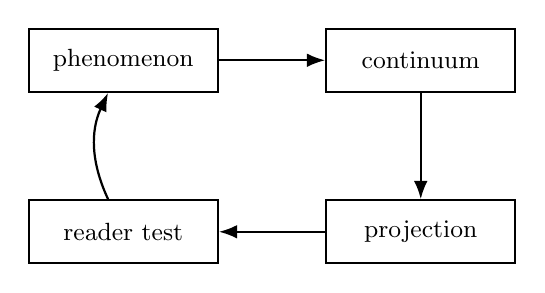
\begin{tikzpicture}[node distance=1.35cm,>=Latex,every node/.style={font=\small}]
\node[draw,thick,align=center,minimum width=2.4cm,minimum height=0.8cm] (a) {phenomenon};
\node[draw,thick,align=center,minimum width=2.4cm,minimum height=0.8cm,right=of a] (b) {continuum};
\node[draw,thick,align=center,minimum width=2.4cm,minimum height=0.8cm,below=of b] (c) {projection};
\node[draw,thick,align=center,minimum width=2.4cm,minimum height=0.8cm,left=of c] (d) {reader test};
\draw[->,thick] (a) -- (b);
\draw[->,thick] (b) -- (c);
\draw[->,thick] (c) -- (d);
\draw[->,thick,bend left=25] (d) to (a);
\end{tikzpicture}
\caption{Operator Catalog Necessity Arguments: state transition of conceptual dependency pressure 36-1-31}
\label{fig:figure-operator-catalog-and-necessity-arguments-one}
\end{figure}
The point of the diagram is not decoration; it marks which relation is being proposed and which stronger conclusion is still unavailable.\par
A local clarification is useful here\par
A local clarification is useful here\footnote{In Operator Catalog Necessity Arguments, this note clarifies the reader clarification role of the term and keeps the caveat close to the sentence that needs it.}.\par
The note keeps the caveat near the term without derailing the main sentence.\par
Consider a hospital during a regional emergency. The hospital is a building, an institution, a legal entity, a workforce, a set of machines, a triage practice, and a public trust. If the electricity fails, one relation is stressed. If staff cannot reach the building, another is stressed. If trust collapses after false reports, another kind of relation is stressed. If all beds are filled, a capacity continuum is approached. If clinicians disagree over triage priority, a normative continuum is activated. A sentence such as the hospital is failing hides these distinctions. A disciplined account must say which continuum is changing, which boundary is crossed, and which operation has altered the configuration.\par
The same difficulty appears far from medicine. A lake can be called healthy, degraded, resilient, or dying, but these words do not yet say whether the relevant change concerns nutrient concentration, species composition, oxygen levels, shoreline use, seasonal circulation, or the relation among all of them. A legal order can be called stable or unstable, but the phrase may point to courts, enforcement, recognition, obedience, legitimacy, or the continuity of persons under law. The language of systems becomes powerful only when it stops treating the system as self-evident.\par
The operator catalog answers this need by naming repeatable forms of transformation. An operator, in this monograph, is not a machine part or a mathematical symbol alone. It is a named operation that changes, relates, projects, binds, separates, stabilizes, or destabilizes a configuration under stated conditions. The word catalog matters because no single operator can carry the whole theory. Some operations mark boundaries. Some compose objects. Some split them. Some move a description from one domain to another. Some expose contradiction. Some register collapse. Later scientific claims can depend on these operators only if the operators have first been made intelligible at the level of ordinary cases.\par
The necessity argument is the companion to the catalog. It asks why these operators are needed rather than merely convenient. A theory can always invent vocabulary. The harder question is whether the vocabulary answers a real structural demand. If a system is described along continua, then there must be some way to say where a description is localized, how a boundary is drawn, how multiple continua are held together, how conflict between descriptions is represented, how a new dimension becomes available, and how a configuration ceases to sustain itself. The argument is not that the chosen names are sacred. It is that the jobs they perform cannot simply be omitted without losing the ability to state the theory's central claims.\par
This makes the catalog a bridge between intuition and formal work. Before equations, simulations, comparisons, or domain projections can be evaluated, the reader needs to know what kind of act is being performed by each operator. A boundary operator does not have the same role as a projection operator. A composition operator does not have the same role as a collapse operator. An operator that helps describe the emergence of a new dimension is not evidence that emergence has occurred in a given case. It supplies a controlled way to say what would have to be shown.\par
The local problem is therefore one of disciplined transfer. OC seeks to compare systems across domains without pretending that the domains are identical. Integrated information theory, associated with Giulio Tononi, is relevant here not because OC adopts its measures, but because it shows how much turns on the problem of integration: what makes many parts count as one experience, one state, or one system rather than as a heap of separable events. Work on critical transitions by Marten Scheffer and collaborators is relevant for a different reason: it presses the question of how a system can appear continuous while approaching a shift in regime. Early warning indicators discussed by Vasilis Dakos and colleagues add methodological pressure, because they show both the appeal and the danger of reading patterns as signs of coming transformation. Derek Parfit's work on persons and reasons enters from another side, showing that identity and persistence can become unstable even when ordinary speech treats them as settled. These neighboring problems do not prove OC. They show why boundary, continuity, integration, transformation, and evidence must be handled with care.\par
\section{Axes Before Continua In Operator Catalog Necessity Arguments}
The catalog begins where confusion usually begins: with the object of description. In ordinary speech, the hospital seems already given. One can point to it, name it, sue it, enter it, fund it, evacuate it, or praise it. Yet the same name covers several objects that do not fail in the same way. The building may remain intact while the care process fails. The legal entity may persist while public trust breaks. The beds may exist while the staffing relation that makes them clinically useful disappears. The first discipline is therefore not to define the hospital once and for all, but to identify the portion of the system being described under a stated perspective and range of variation. That portion is a local configuration. \cite{tononi_information_integration,scheffer_critical_transitions}\par
A local configuration is local because no description captures everything at once. The emergency hospital can be described as an energy-dependent facility, a clinical triage process, a legal responsibility, a social symbol, or a logistical node. Each description is partial. Each may be legitimate. Confusion begins when one partial description silently claims authority over the others. Localization is the operation that selects the configuration and the relevant axes. It may select the intensive care unit rather than the whole hospital, oxygen supply rather than all resources, or staff decision flow rather than equipment. Localization is not a casual narrowing of attention. It is the act that makes a claim testable in principle. A claim about the whole hospital may be too broad; a claim about oxygen delivery during a six-hour interval may be narrow enough to inspect.\par
The local dependency can now be written without changing the claim it supports.\par
\begin{equation}\label{eq:equation-operator-catalog-and-necessity-arguments-two}
\operatorname{historicalInheritance}_{8} = \rho_{\mathrm{replay}}=\frac{N_{\mathrm{matched}}}{N_{\mathrm{declared}}}
\end{equation}
The relation names a local dependency, variable dictionary, and proof/evidence role; it is not a claim-status upgrade.\par
The formula is a restraint on the prose. It names the dependency that the surrounding paragraph is allowed to use.\par
The comparison below gives operator catalog necessity arguments a set of quantities that can be inspected instead of merely admired.\par
\begin{table}[htbp]
\centering\small
\caption{Operator Catalog Necessity Arguments: observable quantities and counter-pressure 36-2-31}
\label{tab:table-operator-catalog-and-necessity-arguments-one}
\begin{tabular}{@{}llll@{}}
\toprule
Proof object & Dependency & Lean surface & Closure state \\
\midrule
operator catalog necessity arguments boundary & 15 units & declared case & fixes what is compared \\
residual pressure & 0.35 & dimensionless & shows unresolved load \\
projection loss & 0.55 & bounded interval & marks lost structure \\
countercase set & 10 cases & review sample & keeps a falsifier visible \\
\bottomrule
\end{tabular}
\end{table}
The table should be read locally: it narrows the comparison without pretending that the wider theory has been settled by a single surface.\par
Once a configuration has been localized, a second need appears. The account must say how the configuration is distinguished from what surrounds it. The boundary of the hospital is not only its wall. The legal boundary of responsibility may extend to ambulance routing. The clinical boundary may extend to patients not yet admitted. The information boundary may include radio dispatch, patient records, and public alerts. The trust boundary may extend into the surrounding community. A boundary operator states the separation rule. It identifies what difference is being used to separate inside from outside for the purpose at hand. Without such a rule, any later claim can be rescued by moving the case outward or inward after difficulty appears.\par
A third need appears as soon as the account says that something is changing. It must identify the direction of variation. Capacity can rise or fall. Integration can tighten or loosen. Permeability can increase or decrease. Latency can shorten or lengthen. Legibility can clarify or degrade. These are axes. An axis does not have to be numerical in every domain, but it must be disciplined enough that movement along it is not arbitrary. If hospital capacity is described, the account must say whether capacity refers to beds, staff, oxygen, operating rooms, decision bandwidth, or some composed measure. If it cannot say that, it has not introduced an axis; it has introduced a mood.\par
The axis opens onto a continuum, an ordered field of possible variation along one or more directions. The term allows a description to avoid false binaries. A boundary is not always simply open or closed. It may be porous, selectively permeable, delayed, contested, or unstable. Integration is not merely present or absent. A workforce can be formally integrated through command structure while practically fragmented by fatigue, distrust, or incompatible information systems. The continuum gives the operator catalog room to describe degrees and transitions without pretending that every degree is already measured.\par
The hospital is not made of axes alone. Its relevant object often lies in the relation among parts. Beds, staff, oxygen, transport, communication, and triage rules may compose a care-delivery configuration. A composition operator describes how multiple elements or axes are held together as one configuration. Composition does not assert harmony. It states the relation through which parts are treated as jointly relevant. This matters because systems often fail not through the total disappearance of parts, but through a breakdown in their relation. The beds may exist, the staff may exist, and the oxygen may exist, while the composed capacity fails because timing and coordination break.\par
The ecological example makes the same need visible without simply repeating the hospital case. A lake is not described adequately by water volume alone, nor by one species count, nor by a single chemical measure. A clear-water lake may depend on a relation among nutrient load, plant cover, fish populations, oxygen, and seasonal mixing. A change in one element may be absorbed; a change in the relation among elements may alter the regime. Scheffer's work on critical transitions gives this problem its precise pressure: systems can remain recognizable across gradual change and then reorganize sharply when resilience is lost. OC does not inherit the empirical models of lake ecology by analogy. It learns from the problem of how composed relations can matter more than isolated variables.\par
Projection becomes necessary when the account tries to move from one domain to another. A projection operator moves a description from one domain, scale, or vocabulary into another while preserving an explicit relation and losing whatever cannot lawfully be carried. A model of ecological resilience cannot simply be copied into political order, and a theory of personal identity cannot simply be treated as a theory of institutional continuity. Projection requires discipline about what is retained. Scheffer's discussion of critical transitions can inform how one thinks about thresholds and resilience, but it does not license the claim that every social crisis has the same structure as a lake changing state.\par
The next problem is not mere stress. Systems endure stress constantly. A busy emergency department is under tension. A lake under seasonal variation is under tension. A legal order containing disagreement is under tension. Tension is a strain between axes, constraints, or descriptions that can still be held within the configuration. Contradiction, in the stronger OC sense, is narrower. It is an unresolved incompatibility that the configuration cannot absorb under its current dimensional description. A triage protocol that simultaneously requires mutually exclusive priorities under the same conditions may create contradiction. A legal system may tolerate competing interests, but it may not sustain an operative rule that both includes and excludes the same class of persons under the same condition and in the same respect.\par
The central hypothesis can now be stated more carefully. OC treats unresolved contradiction as a candidate source of either dimensional transformation or structural failure. The hypothesis is not an established law of nature, and it does not claim that every conflict produces novelty or collapse. It says that when a configuration cannot sustain an incompatibility within its existing axes, two theoretical outcomes become especially important to distinguish. The description may acquire a new dimension that reorganizes the relations at stake, or the configuration may lose the operative relations that made it the configuration under analysis. Particular cases must still earn either claim through evidence, formal derivation, or disciplined comparison.\par
Emergence names the first of these possible outcomes, but the word must be kept narrow. A new label is not enough. A new rule is not enough. A new category in an administrative table is not enough. An emergence operator marks the appearance of a new dimension of description when the previous descriptive space cannot represent the needed distinctions. In the hospital case, an overload may initially appear as a capacity problem. As the emergency deepens, clinicians may develop a triage dimension that changes how patients, resources, and obligations are related. The new dimension does not make the suffering less real. It changes the operational space in which decisions can be described.\par
A legal example helps test the distinction. Suppose a legal order classifies persons by a fixed civil status, but a new class of cross-border dependency appears that the old status categories cannot represent: people are subject to obligations, affected by decisions, and exposed to enforcement while lacking the recognition through which those relations can be answered. Merely adding a label for the group would not be emergence in the relevant sense. A new dimension appears only if the legal description must now track a relation such as affected standing, derivative obligation, or distributed personhood, and if that dimension changes what counts as inclusion, exclusion, duty, and remedy. Emergence is not naming. It is a change in the space of possible relations.\par
Collapse names the second possible outcome. A collapse operator marks the loss of a configuration's ability to sustain its operative relations. Collapse is not every failure, nor every bad outcome. A temporary shortage is not collapse if the configuration can recover within its existing relations. A collapse occurs when the relations that made the configuration count as that configuration no longer hold. A hospital that loses one ward is damaged. A hospital that can no longer coordinate care, preserve clinical authority, or distinguish patients by any workable triage process may have undergone a structural collapse in the relevant description. A lake that becomes turbid after a storm has not necessarily collapsed; a lake that reorganizes into a persistent state in which the former clear-water relations cannot reassert themselves may be a better candidate.\par
The catalog also needs identity and persistence operators. Parfit's analysis of personal identity is useful here because it separates survival, psychological continuity, and ordinary identity talk in ways that unsettle simple assumptions. OC does not need to adopt Parfit's conclusions to learn from the problem. A system can persist materially while losing functional identity, or preserve a name while changing the relations that once made the name accurate. A corporation, a research program, a city, or a person can remain continuous under one description and discontinuous under another. Identity operators state which continuity relation is being used.\par
\section{Operators And Their Burden In Operator Catalog Necessity Arguments}
The operator catalog is not derived from an aesthetic preference for systematic vocabulary. It follows from the needs created by the theory's own starting point. If a system is described through continua, then several tasks arise before any ambitious claim can be made. The theory must select a local configuration. It must name axes of variation. It must mark boundaries. It must describe how elements compose. It must handle tensions and contradictions. It must distinguish transformation from failure. Any account that lacks one of these tasks may still be interesting, but it cannot carry the full OC claim. \cite{tononi_information_integration,scheffer_critical_transitions}\par
The need for localization is easiest to see when a sentence becomes too large. Saying that modern institutions are unstable, that consciousness is integrated, that ecosystems approach transition, or that identity is continuous leaves too much unspecified. Which institution, under which function, over which interval, and with respect to which boundary? Which aspect of consciousness, under which model of integration? Which ecosystem variable? Which identity relation? The localization operator is necessary because the theory cannot compare configurations unless it first knows what is being compared.\par
The local dependency can now be written without changing the claim it supports.\par
\begin{equation}\label{eq:equation-operator-catalog-and-necessity-arguments-one}
\operatorname{grandSynthesis}_{8} = G=(V_{\mathrm{claim}}\cup V_{\mathrm{evidence}},E_{\mathrm{support}}\cup E_{\mathrm{challenge}})
\end{equation}
The relation names a local dependency, variable dictionary, and proof/evidence role; it is not a claim-status upgrade.\par
The formula is a restraint on the prose. It names the dependency that the surrounding paragraph is allowed to use.\par
The local dependency can now be written without changing the claim it supports.\par
\begin{equation}\label{eq:equation-operator-catalog-and-necessity-arguments-three}
\operatorname{methodFalsifier}_{8} = \epsilon_{\mathrm{domain}}=\max_i |y_i-\hat y_i|
\end{equation}
The relation names a local dependency, variable dictionary, and proof/evidence role; it is not a claim-status upgrade.\par
The formula is a restraint on the prose. It names the dependency that the surrounding paragraph is allowed to use.\par
A small numerical test keeps the abstraction honest at the scale of a single decision.\par
\paragraph{Numerical example.} For operator catalog necessity arguments, take support=0.60, projection loss=0., and 5 open obligations. The bounded score is 0.; the example gives the reader a numeric scale without pretending to be empirical proof.\par
The numbers are deliberately small; their value is pedagogical, not evidential, unless the chapter binds them to a dataset elsewhere.\par
Tononi's work sharpens this demand by making integration central to a theory of consciousness. Whatever one thinks of the formal measure, the conceptual pressure is clear: the theory cannot be satisfied with a loose claim that many parts are active. It must ask under what conditions many components count as integrated. OC borrows no result from that framework, but it takes seriously the problem that integration cannot be gestured at from a distance. The configuration must be selected, and the relation that makes it one rather than many must be stated.\par
A local configuration without axes is a named region with no structured variation. It may be described, but it cannot be examined as a continuum. The axis operator is necessary because OC claims involve movement, pressure, threshold, resolution, and collapse. These are not meaningful unless something can vary. A hospital does not move toward collapse in the abstract. Its staffing ratio changes, supply reliability changes, information latency changes, public trust changes, and decision authority changes. The axes give those changes grammar.\par
Boundary marking follows because axes do not float freely. They belong to descriptions of configurations that are separated from surrounding conditions for a reason. A boundary operator is necessary because every later claim depends on what is counted inside the case. Suppose a hospital cannot discharge patients because no long-term care facilities are available. Is that hospital capacity failure, regional care-network failure, or both? The answer depends on the boundary. A theory that refuses to declare boundaries can always shift the object after the fact. That flexibility may sound generous, but it weakens the claim.\par
Composition is necessary because many systems are not reducible to isolated variables. The relevant object is often a relation among parts. Oxygen supply alone does not define care capacity. Staff alone do not define it. Beds alone do not define it. A composed care-capacity configuration exists only when these elements are coordinated through timing, authority, information, and physical access. The composition operator is therefore not ornamental. It states how many partial continua become one operative configuration for the claim being made.\par
The same logic applies to ecological cases. Nutrient concentration, plant coverage, predator balance, and water clarity are individually describable, but the system of interest may be a composed relation among them. Scheffer's studies of regime shifts place pressure exactly here: the object is not a single variable moving smoothly, but a configuration whose resilience may weaken before its visible state changes. OC does not claim that every composed system has ecological resilience in the technical sense. It uses the ecological problem to show why composition and transition must be kept distinct from a list of parts.\par
Projection is necessary because OC is a language about how domains can be described, compared, and bounded, rather than a claim that one domain's objects are secretly the same as another's. Without projection operators, cross-domain comparison becomes either reckless analogy or sterile isolation. Reckless analogy says the hospital is like an ecosystem, therefore it must behave like one. Sterile isolation says hospitals and ecosystems share nothing because their observables differ. Projection offers a third route: it asks which structural relation can be carried and what must be left behind.\par
Dakos and colleagues add a caution that is crucial for this route. Early warning signals can be powerful, but they are not magic signatures that free the observer from domain knowledge. Rising variance, autocorrelation, or other indicators may matter in one setting and mislead in another. For OC, that warning becomes a rule of projection. A pattern may suggest a question about approach to transition; it does not by itself license a conclusion about collapse, emergence, or causality. Projection must preserve the question without smuggling in the answer.\par
Contradiction handling is necessary because the central hypothesis concerns unresolved contradiction, but the hypothesis must be held within strict limits. It is a theoretical proposal about what may happen when a configuration cannot absorb an incompatibility under its current dimensional description. Ordinary conflict is too broad. Stress, scarcity, disagreement, delay, and ambiguity are not yet contradiction in the strong sense. The operator must mark when a configuration's current axes cannot jointly sustain the requirements placed on them.\par
Emergence and collapse operators are necessary because the theory distinguishes two possible outcomes of unresolved contradiction. If the contradiction is addressed by adding a new dimension of description, the system has not merely changed value along an old axis. It has changed the descriptive space. If the contradiction cannot be addressed and the operative relations fail, the system has not merely suffered a local loss. It has collapsed with respect to the configuration under description. These two outcomes are not interchangeable. A catalog that lacks one of them would force unlike cases into the same language.\par
The derivation route also explains why necessity arguments must remain modest. A necessity argument can show that a theoretical role must be filled. It cannot show that a particular empirical system has undergone the transformation named by that role. The fact that a collapse operator is needed does not show that any named civilization, institution, organism, or model has collapsed. The fact that an emergence operator is needed does not show that a new dimension has appeared in a given dataset. The catalog prepares claims; it does not certify them.\par
Parfit's work helps clarify the same modesty in the domain of identity. The familiar question whether a person remains the same through psychological change, bodily change, or branching continuity cannot be solved by a slogan about persistence. It requires the relation of continuity to be named. OC uses that pressure to separate material persistence, functional persistence, legal persistence, narrative persistence, and moral concern. The lesson is not that a hospital, lake, legal order, and person are the same kind of thing. The lesson is that identity claims become unstable when the continuity relation is left unspoken.\par
\section{A Claim Made Inspectable In Operator Catalog Necessity Arguments}
Even when no equation is required in a section, the prose must prepare the surface on which equations could later appear. An equation surface is the disciplined interface between ordinary explanation and formal expression. It does not mean that every term is already mathematical. It means that the language has been constrained enough that later formalization will not have to guess what the prose meant. If an operator is named, its object, input, output, and limiting conditions must be at least conceptually visible. \cite{tononi_information_integration,scheffer_critical_transitions}\par
Take localization. In ordinary prose, one might say that attention narrows to the emergency department. For formal work, the same move would need a local configuration selected from a broader system under a description. The prose therefore has to say what is being selected and why. It cannot simply gesture at the emergency department as an obvious object. Is the local object a physical area, a staffing pattern, a flow of decisions, or a care-delivery function? The later formal surface depends on that answer.\par
The case that follows turns the proposal into a sequence of criticizable moves.\par
\paragraph{Worked case.} In the worked case for operator catalog necessity arguments, the claim is reduced to a boundary, an observable, a dependency, a numerical cue, and a falsifier. The case is useful only because each move can be criticized separately.\par
The case helps because each step can fail separately, which is exactly what a useful example should permit.\par
The same is true for boundary marking. If a boundary operator is later expressed in formal notation, it must not be asked to repair vagueness that prose left unresolved. The hospital wall, the legal jurisdiction, the patient intake system, and the public communication channel define different boundaries. A formal symbol for boundary cannot make them equivalent. It can only operate on a boundary already specified by the theory. This is why the public language must remain concrete before it becomes compressed.\par
Composition also demands discipline. A composed configuration can be treated as a structured object only if its components and relations have been identified. Beds plus nurses plus oxygen plus ambulance arrivals is still not a care-delivery configuration unless timing, assignment, and authority relations are included. A later formal expression might represent a composition operation, but the expression would be empty if the prose had not explained the relation that makes composition meaningful.\par
Projection is especially vulnerable to misuse. A projection operator may later be formalized as a mapping between descriptions, but the word mapping can hide too much. What is preserved? What is discarded? What kind of distortion is accepted? If ecological resilience is projected into institutional analysis, variables cannot be carried as if they were identical. An algae-dominated lake and a hospital network do not share the same observables. What can be carried is a more abstract relation among stability, disturbance, threshold, and reorganization, and even that relation must be limited by domain differences.\par
Contradiction requires the strictest care. A contradiction operator cannot be a dramatic synonym for stress. In a formal setting, contradiction must indicate incompatibility under a defined description. For the hospital, a contradiction might arise if the operative rule requires immediate treatment for all critical patients while the resource relation makes simultaneous treatment impossible and no prioritization dimension exists. Once a triage dimension is introduced, the description changes. The contradiction may be transformed into a tragic but structured decision space. That transformation is not moral absolution; it is an ontological change in the description.\par
Emergence, likewise, must not be treated as a decorative word for novelty. A new label, new policy, or new observation is not necessarily a new dimension. The emergence operator is reserved for cases where the previous descriptive space cannot represent the needed distinctions, and a new axis or relation becomes necessary. In the hospital example, a new triage category may be emergent only if it changes the space of possible decisions rather than merely renaming an existing priority. In the legal example, a new status label is not enough; the relations of obligation, recognition, remedy, and standing would have to be reorganized by a dimension that the old scheme could not express.\par
Collapse must be equally constrained. A downturn, shortage, scandal, or failure may be severe without being collapse in the OC sense. Collapse marks a failure of operative relations within the local configuration. A hospital can be overwhelmed and still operate under recognizable care relations. It can lose a department and remain a hospital. The collapse operator becomes relevant when the configuration can no longer sustain the relations that made it count as the object under analysis. The difference is not rhetorical; it determines what later claims are allowed to say.\par
The same discipline applies when the case is ecological. A lake may suffer pollution without collapsing as the configuration under description. It may recover through seasonal circulation, intervention, or remaining biological relations. Collapse becomes relevant only if the operative relations that sustained the prior regime no longer hold. If the claim concerns a regime shift, then the axes, boundaries, and composed relations must be named. Otherwise the language of collapse merely dramatizes degradation.\par
An equation surface therefore performs a public service before any symbols appear. It forces the prose to identify objects and operations with enough stability that the reader can later recognize the formal version. It also prevents a common mistake in speculative theory: using formal notation to create an appearance of precision after the underlying terms have remained loose. OC cannot rely on that move. Its operators must be intelligible before they are formalized, and any later formalization must answer back to the meanings established here.\par
This also explains why no equation is needed at this point. The necessary work is conceptual compression, not calculation. A premature formula could make the catalog look more settled than it is. The scientific discipline lies in refusing both extremes: loose metaphor on one side and premature mathematical display on the other. The operator catalog stands between them. It makes the claims more exact without pretending that all domains already share a common measurement regime.\par
\section{What The Formula Does Not Prove In Operator Catalog Necessity Arguments}
The catalog must carry a burden that ordinary terminology cannot carry. It must let a reader distinguish the existence of a theoretical role from the truth of a particular application. This distinction is the difference between a usable operational language and a vocabulary that merely sounds general. If the theory says that contradiction may lead to emergence or collapse, the operator catalog must say what contradiction, emergence, and collapse mean before any case is judged. Otherwise the central hypothesis becomes too easy to satisfy. \cite{tononi_information_integration,scheffer_critical_transitions}\par
The burden begins with necessity. Why not speak only of causes, effects, systems, and outcomes? The answer is that those terms do not preserve the distinctions OC needs. Cause and effect can describe an event sequence, but they may not identify the continuum along which the system varies. System can name a whole, but it may not specify the boundary that made the whole local. Outcome can describe what happened, but it may not distinguish transformation within an old descriptive space from the appearance of a new dimension. The operators are necessary because they prevent these differences from being lost.\par
A skeptical reader might object that the catalog adds terminology where ordinary analysis would do. The objection has force. A theory should not multiply terms for display. The answer is practical: each operator must earn its place by doing work that ordinary terms leave underspecified. If boundary, projection, composition, contradiction, emergence, and collapse are used carelessly, the objection wins. If they allow claims to be narrowed, rejected, compared, or transferred with fewer hidden assumptions, then the added vocabulary is justified.\par
Another objection concerns cross-domain ambition. A language that can speak about hospitals, ecosystems, persons, and institutions may appear too broad to be scientific. The danger is real. The answer is not to deny it, but to impose limits on projection. OC does not claim that all domains share the same substance, measurements, or evidential standards. It claims that some operational questions recur: what is the local configuration, what varies, where is the boundary, how are parts composed, what cannot be jointly sustained, and what happens when the configuration changes or fails? The breadth belongs to the questions, not to an automatic equivalence among answers.\par
A third objection concerns evidence. If the catalog is necessary, does that establish the theory? No. It establishes only the need for certain roles within the theory. Evidence would have to come from particular cases, simulations, datasets, comparisons, or formal results, each with its own limits. The catalog cannot borrow authority from later evidence, and later evidence cannot repair an unclear catalog. They are different tasks. This separation is central to the monograph's scientific status.\par
The neighboring literature helps clarify the burden without carrying it for OC. Tononi's integrated information theory shows how a theory can make integration central and then face demanding questions about formal definition and empirical interpretation. Scheffer's work on critical transitions shows how systemic change can be studied through resilience, thresholds, and regime shifts. Dakos and colleagues show that early warning signals can be discussed with methodological care, including the risk of overinterpretation. Parfit shows that identity can be philosophically unsettled even in cases where ordinary language remains confident. These works do not supply OC's operators. They show that the problems to which the operators respond are not invented for convenience.\par
The catalog must also keep moral, scientific, and ontological claims distinct. In the hospital example, triage may introduce a new decision dimension. That does not make the situation morally acceptable. A structural description of collapse does not assign blame by itself. A continuity operator may show that an institution persists under one description and fails under another, but it does not decide whether the institution deserves trust. OC's operators organize description; they do not automatically settle ethical or political judgment.\par
This point matters because terms such as contradiction, emergence, and collapse carry emotional force. They can make an argument sound more dramatic than the evidence warrants. The catalog must drain some of that drama by making each term harder to use. A contradiction must be located. Emergence must introduce a new dimension, not merely a new event. Collapse must refer to operative relations, not just loss or decline. Projection must state what is carried and what is not. Boundary must be declared rather than assumed.\par
The argument burden, then, is two-sided. The catalog must be strong enough to support later claims, but strict enough to block inflated ones. It must allow the theory to say more than ordinary description, but it must also make some tempting sentences unlawful within the theory's own discipline. If a claim cannot name its local configuration, axes, boundary, composition, and operator, then the catalog gives the reader a reason to suspend acceptance. That is not a weakness of the theory. It is the cost of making the language inspectable.\par
\section{The First Formal Move In Operator Catalog Necessity Arguments catalogS}
The operator catalog also defines where the theory fails. This is not a pessimistic appendix to the argument; it is part of the argument's honesty. A theory that cannot say when its own language has been misused becomes unfalsifiable in practice even if it sounds careful in principle. The failure boundary marks the point at which an OC description has lost enough discipline that it no longer deserves the authority of the framework. \cite{tononi_information_integration,scheffer_critical_transitions}\par
The first failure boundary is unlocalized speech. If a claim says that a system is collapsing but cannot identify the local configuration, the claim fails at the catalog level. It may be a warning, a metaphor, or a political judgment, but it is not yet an OC claim. The same applies to statements about emergence, contradiction, or integration. Without localization, there is no object for the operator to operate on.\par
The second boundary is axis vagueness. A claim fails when it says that a configuration is moving, intensifying, weakening, or transforming without naming the dimension of variation. In the hospital example, saying that pressure increased is not enough. Did patient volume increase, staff availability decrease, oxygen reliability degrade, decision latency lengthen, or public trust erode? Each answer changes the analysis. Axis vagueness allows a theory to appear explanatory while avoiding the question of what actually changed.\par
The third boundary is boundary drift. A description fails when it changes the inside and outside of the case whenever difficulty appears. If hospital capacity is defined narrowly at first and then expanded to include regional elder care only after the claim is challenged, the analysis may still be repairable, but the shift must be acknowledged. Boundary changes are allowed; silent boundary changes are not. The operator catalog requires the boundary to be part of the claim, not a convenience used after the fact.\par
The fourth boundary is projection inflation. A projection fails when it carries more from one domain to another than the relation permits. It is legitimate to compare certain threshold patterns in ecology and institutions at a high level of abstraction. It is not legitimate to treat a social institution as if it had the same observables, causal mechanisms, or evidential standards as an ecological system. Projection inflation is one of the easiest ways for a cross-domain theory to overstate itself. The catalog blocks it by forcing every projection to declare its preservation and loss.\par
The fifth boundary is contradiction inflation. Not every conflict is a contradiction. Not every contradiction is unresolved. Not every unresolved contradiction produces emergence or collapse in an observable way. A hospital under strain may adapt within existing categories. A legal system may contain tensions for long periods. A person may live with incompatible self-descriptions without forming a new identity dimension or suffering collapse. The strong OC claim begins only when incompatibility cannot be sustained under the current description.\par
The sixth boundary is emergence inflation. Novelty is common. New labels, procedures, and events appear constantly. Emergence in the catalog's sense is narrower. It requires a new dimension of description that changes the space of possible relations. If a hospital renames a ward, that is not emergence. If it develops a new triage dimension because the old patient categories cannot represent the operative conflict, emergence may be considered. If a legal order coins a new administrative label without changing the relations of standing, obligation, recognition, and remedy, that is not emergence in this sense. The distinction keeps the term from becoming a reward for interesting cases.\par
The seventh boundary is collapse inflation. Collapse is not a synonym for harm, failure, injustice, exhaustion, or decline. These may accompany collapse, but they do not define it. Collapse concerns the failure of operative relations that sustain the local configuration. A department closure may be grave but local. A temporary overload may be survivable. A structural collapse occurs when the configuration can no longer operate as the kind of configuration under analysis. The operator requires that distinction even when ordinary speech would not.\par
The final boundary is evidential overreach. The catalog can make a claim possible, coherent, and bounded. It cannot make it true by itself. A later empirical claim must still answer to its evidence. A later formal claim must still answer to its definitions and derivations. A later comparison must still answer to the differences between domains. The catalog has done its job when it makes these demands visible before the reader reaches them.\par
This is why the chapter ends not with a triumphant claim for the operators, but with a stricter sense of what they permit. They permit the reader to ask whether a configuration has been localized, whether its axes have been named, whether its boundary has been declared, whether its parts have been composed by an explicit relation, whether a projected comparison has preserved only what it may preserve, whether contradiction has been distinguished from tension, whether emergence has added a dimension rather than a label, and whether collapse has been tied to operative relations rather than to rhetorical severity.\par
The handoff is therefore precise. The reader now has the local problem, the basic objects, the operator families, the derivation route, the interface with later formal expression, the burden carried by necessity arguments, and the failure conditions that keep the vocabulary from inflating. Later claims about continua, contradiction, emergence, collapse, evidence, simulation, comparison, and domain projection can now be read against this standard. The operator catalog does not ask for trust in advance. It gives the reader the terms by which trust can be earned, narrowed, or withdrawn.\par
\chapter{First Formal Summary Before K-Levels}
\section{The First Formal Move In First Formal Summary Before}
Before the book turns to K levels, the later vocabulary for layered organization, it has to slow down over a more ordinary question: what is being measured when something is said to remain itself, change itself, or lose itself? OC, short for Organic Computation, uses that question to discipline description before it asks larger claims to carry weight. A lake, a legal norm, an institution, a nervous system, and a city transit system do not offer the same evidence. They do not change in the same way. Still, in each case a reader can ask what must persist for the thing under discussion to remain the same organized thing. \cite{scheffer_critical_transitions,dakos_early_warning}\par
Take the lake first, because it gives the problem a visible shape. In one season it is clear enough for plants to root across the shallows. Light reaches the bottom. Fish, plants, sediment, nutrients, and inflows hold one another in a recognizable arrangement. In another season the same basin may still be there, the same map may still name it, and yet the water may be thick with algae. Light no longer reaches the plants. Sediment is disturbed more easily. The relations that once kept the lake clear no longer support that form of lake life.\par
The next diagram slows the argument down just enough to show how first formal summary before is being organized.\par
\begin{figure}[htbp]
\centering
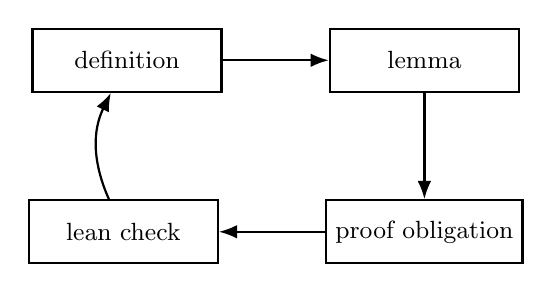
\begin{tikzpicture}[node distance=1.35cm,>=Latex,every node/.style={font=\small}]
\node[draw,thick,align=center,minimum width=2.4cm,minimum height=0.8cm] (a) {definition};
\node[draw,thick,align=center,minimum width=2.4cm,minimum height=0.8cm,right=of a] (b) {lemma};
\node[draw,thick,align=center,minimum width=2.4cm,minimum height=0.8cm,below=of b] (c) {proof obligation};
\node[draw,thick,align=center,minimum width=2.4cm,minimum height=0.8cm,left=of c] (d) {lean check};
\draw[->,thick] (a) -- (b);
\draw[->,thick] (b) -- (c);
\draw[->,thick] (c) -- (d);
\draw[->,thick,bend left=25] (d) to (a);
\end{tikzpicture}
\caption{First Formal Summary Before: residual plot of proof dependency pressure 37-1-32}
\label{fig:figure-first-formal-summary-before-k-levels-one}
\end{figure}
The point of the diagram is not decoration; it marks which relation is being proposed and which stronger conclusion is still unavailable.\par
A local clarification is useful here\par
A local clarification is useful here\footnote{In First Formal Summary Before, this note clarifies the reader clarification role of the term and keeps the caveat close to the sentence that needs it.}.\par
The note keeps the caveat near the term without derailing the main sentence.\par
The question is not whether the lake has vanished. It has not. Nor is the question whether every change is a loss of identity. Seasonal variation is part of the lake's life. A hot week, a storm, a small nutrient pulse, or a shift in fish population may alter the lake without destroying the clear-water organization. The harder question is where ordinary variation ends and a different organization begins. That is the kind of question OC wants to make answerable rather than merely emphatic.\par
For that purpose, a configuration is not a bare object. It is the system as described along selected ranges of variation, inside a stated boundary, under a stated operation or comparison. The term is deliberately plainer than it may first sound. It says that a lake described as an ecological regime is not the same formal object as a lake described as a recreational site, a regulated water body, a property asset, or an image in local memory. These descriptions may overlap, but they cannot be exchanged without cost.\par
Research on critical transitions makes the lake example especially useful. Marten Scheffer and colleagues have shown how ecosystems can approach thresholds where small disturbances have large effects, and where the return from disturbance can slow as a transition nears. Vasilis Dakos and colleagues have studied early-warning indicators that sometimes appear before such shifts. OC does not borrow those findings as proof of its own framework. It borrows a limited lesson: in serious descriptions of change, one must say which system, which variables, which disturbances, and which boundaries make the claim meaningful.\par
A clear lake can therefore remain the same in one sense while changing in another. Its basin can persist while its ecological organization fails. Its legal status can remain stable while its biological relations change. Its recreational value can decline before the ecological state has crossed a threshold, or ecological change can be well underway before casual observers notice. The word same is too small to carry all of this. It needs help from a declared frame.\par
The quantity under discussion in OC is the described state of such a framed configuration. It is not always a number, though numbers may enter. It is not a hidden essence behind the evidence. It is the organized condition that a claim is actually about. Once this is made explicit, later words such as persistence, emergence, collapse, and contradiction have less room to drift. They have to answer to a stated object.\par
\section{Axes Before Continua In First Formal Summary Before}
A compact notation helps only after the reader has something concrete in mind. Let S name the system being discussed. Let C name the continuum, or family of continua, along which the system is being described. Let B name the boundary that determines what counts inside the present description and what is left outside it. Let O name the operation by which the system is changed, tested, compared, measured, or interpreted. Let x name the resulting state or configuration of S as described through C, B, and O. \cite{scheffer_critical_transitions,dakos_early_warning}\par
The symbols should be read as a guard against confusion, not as a claim that ecology, law, psychology, and economics secretly share one numerical substance. S is simply the selected system, not the whole world. C is the relevant range of variation, not reality itself. B is a boundary condition, not necessarily a wall. O is an action, comparison, disturbance, or interpretive move, not always a mechanical force. x is the described configuration, not an inner soul of the system.\par
The local dependency can now be written without changing the claim it supports.\par
\begin{equation}\label{eq:equation-first-formal-summary-before-k-levels-two}
\operatorname{dimensionalBirth}_{8} = \kappa_{K_8}=\frac{b_{K_8}+s_{K_8}}{1+o_{K_8}+q_{K_8}}
\end{equation}
The relation names a local dependency, variable dictionary, and proof/evidence role; it is not a claim-status upgrade.\par
The formula is a restraint on the prose. It names the dependency that the surrounding paragraph is allowed to use.\par
The comparison below gives first formal summary before a set of quantities that can be inspected instead of merely admired.\par
\begin{table}[htbp]
\centering\small
\caption{First Formal Summary Before: observable quantities and counter-pressure 37-2-32}
\label{tab:table-first-formal-summary-before-k-levels-one}
\begin{tabular}{@{}llll@{}}
\toprule
Dataset role & Source type & Replay cue & Reader question \\
\midrule
first formal summary before boundary & 18 units & declared case & fixes what is compared \\
residual pressure & 0.42 & dimensionless & shows unresolved load \\
projection loss & 0.66 & bounded interval & marks lost structure \\
countercase set & 11 cases & review sample & keeps a falsifier visible \\
\bottomrule
\end{tabular}
\end{table}
The table should be read locally: it narrows the comparison without pretending that the wider theory has been settled by a single surface.\par
Return to the lake. If S is the lake as an ecological system, C might include nutrient concentration, turbidity, plant cover, oxygen levels, fish pressure, and recovery after disturbance. B might include the basin, sediment, inflows, and immediate watershed inputs while excluding national politics and tourism marketing. O might be a nutrient pulse, a drought, a measurement protocol, or a comparison between clear-water and turbid-water regimes. x is then the lake's ecological configuration under that description.\par
The same physical place can be described differently without contradiction. If S is the lake as a public amenity, C may include swimming days, odor complaints, visual clarity from the shore, and local access. If S is the lake as a regulatory object, C may include statutory thresholds, inspection records, permitted discharges, and enforcement actions. A claim about ecological collapse cannot be settled by pointing only to unchanged property boundaries. A claim about regulatory failure cannot be settled by one attractive photograph of the surface.\par
This is the point of the notation. It makes the hidden frame visible. When someone says, "the lake is fine," the sentence may mean that the water is still inside the basin, that legal limits have not been exceeded, that tourists still arrive, that fish still live there, or that the clear-water ecological regime is intact. Each claim has a different S, C, B, O, and x. The notation forces the speaker to choose.\par
A legal example shows the same discipline from a different angle. Suppose the system is a constitutional norm. Its continua may include interpretive scope, institutional acceptance, enforcement consistency, conflict with other norms, and public legitimacy. Its boundary may be one jurisdiction over a specified period. Its operation may be a court decision, amendment, administrative practice, or pattern of non-enforcement. The described state is not the text alone. It is the norm as it functions within the declared legal frame.\par
This does not mean that a legal norm behaves like a lake. It means that both cases punish vague speech. A lake may be named while its operative ecology is ignored. A norm may be quoted while its institutional force is gone. In both cases the notation asks the same readerly question: what exactly is being described, along what range of variation, within what boundary, and under what operation?\par
\section{Operators And Their Burden In First Formal Summary Before}
The relation can be written in one line: x = F(S, C, B, O). Read it without grandeur. The configuration being discussed is produced by a way of describing a system, along selected continua, inside a boundary, under an operation. F marks the rule, model, interpretation, measurement procedure, or explanatory practice that connects these elements. It is not a universal engine hidden behind the letter. \cite{scheffer_critical_transitions,dakos_early_warning}\par
The usefulness of the line is practical. It keeps a claim from floating free of the choices that made it possible. If the system changes, the claim changes. If the continuum changes, the claim changes. If the boundary changes, the claim changes. If the operation changes, the claim changes. This is not a defect to be concealed. It is how responsible description becomes open to criticism.\par
The local dependency can now be written without changing the claim it supports.\par
\begin{equation}\label{eq:equation-first-formal-summary-before-k-levels-one}
\operatorname{readerInspection}_{8} = \operatorname{support}(c_{8})=P(c_{8})\wedge E(c_{8})\wedge R(c_{8})
\end{equation}
The relation names a local dependency, variable dictionary, and proof/evidence role; it is not a claim-status upgrade.\par
The formula is a restraint on the prose. It names the dependency that the surrounding paragraph is allowed to use.\par
The local dependency can now be written without changing the claim it supports.\par
\begin{equation}\label{eq:equation-first-formal-summary-before-k-levels-three}
\operatorname{collapseBoundary}_{8} = \operatorname{falsify}(h)=\exists e\in E\,:\,\operatorname{pred}_h(e)\neq\operatorname{obs}(e)
\end{equation}
The relation names a local dependency, variable dictionary, and proof/evidence role; it is not a claim-status upgrade.\par
The formula is a restraint on the prose. It names the dependency that the surrounding paragraph is allowed to use.\par
A small numerical test keeps the abstraction honest at the scale of a single decision.\par
\paragraph{Numerical example.} For first formal summary before, take support=0.43, projection loss=0.13, and 6 open obligations. The bounded score is 0.; the example gives the reader a numeric scale without pretending to be empirical proof.\par
The numbers are deliberately small; their value is pedagogical, not evidential, unless the chapter binds them to a dataset elsewhere.\par
In the lake case, the equation can be felt almost physically. With S as the lake ecology, C as the set of ecological variables, B as the basin plus immediate inflows, and O as a nutrient increase, x may describe movement toward a turbid regime. Widen B to include agricultural policy in the watershed, and the configuration now includes institutional causes and feedbacks. Narrow C to surface clarity alone, and the result becomes easier to measure but less able to explain why the change is occurring. Replace the nutrient pulse with drought, and a different operation is being examined.\par
The line does not tell the ecologist what the lake will do. It tells the writer what must not be smuggled into the sentence. A claim about nutrients should not quietly become a claim about tourism. A claim about the basin should not pretend to explain watershed policy. A claim about one-day appearance should not stand in for recovery dynamics. The equation is a reader's tool for asking whether the sentence has earned its own conclusion.\par
A before-and-after version makes the difference plain. Vague claim: "The lake collapsed because people stopped caring for it." Revised claim: "The clear-water ecological configuration of the lake shifted toward a turbid regime after repeated nutrient inputs exceeded the stabilizing relations among plant cover, sediment, light penetration, and fish pressure within the basin and immediate inflow boundary." The revised sentence is less dramatic, but it is more criticizable. A reader can ask about nutrient records, plant surveys, sediment disturbance, light penetration, fish populations, and the chosen boundary. The sentence has become vulnerable in the right way.\par
The same improvement can happen outside ecology. Vague claim: "The institution failed because trust disappeared." Revised claim: "The enforcement configuration of the institution weakened after a public audit changed compliance behavior among regulated actors, while the formal legal mandate remained intact." Now the institution is not treated as one mysterious object. Enforcement, public confidence, formal authority, and compliance can be separated. The claim may still be false, but it is no longer protected by vagueness.\par
Derek Parfit's work on personal identity offers a neighboring lesson. Parfit argued that questions about being the same person can become clearer when attention shifts to psychological continuity, connectedness, and survival-relevant relations. OC does not turn Parfit's philosophy into a rule for every domain. It borrows the caution that a single noun may hide several relations. A person, practice, institution, or lake is not made formally clear by being named. It becomes clearer when the relations supporting the claim of sameness are brought into view.\par
\section{A Claim Made Inspectable In First Formal Summary Before}
A name gathers attention, but it does not settle comparison. "The lake," "the court," "the market," "the self," and "the theory" can each be spoken as if the object were obvious. Often it is not. The name may cover physical continuity, functional continuity, legal continuity, narrative continuity, or organizational continuity. OC begins by refusing to let one word do all of that work silently. \cite{scheffer_critical_transitions,dakos_early_warning}\par
For the lake, this refusal matters because several true statements can coexist. The basin remains. The water body remains. The clear-water regime may not remain. The recreational season may be damaged before the ecology has fully shifted. The legal designation may remain unchanged long after the actual conditions have altered. None of these statements defeats the others until their frames are confused. The task is not to choose the most forceful phrase. The task is to say which configuration is at stake.\par
The case that follows turns the proposal into a sequence of criticizable moves.\par
\paragraph{Worked case.} In the worked case for first formal summary before, the claim is reduced to a boundary, an observable, a dependency, a numerical cue, and a falsifier. The case is useful only because each move can be criticized separately.\par
The case helps because each step can fail separately, which is exactly what a useful example should permit.\par
This is also where the later idea of contradiction can be introduced without theatrical language. In OC, a contradiction is not any disagreement, difficulty, or ordinary tension. It is a structural incompatibility inside a described configuration that cannot be resolved within the active continua and boundary while preserving the organization under discussion. A lake that warms in summer is not thereby contradictory. A lake that absorbs a moderate nutrient pulse is not thereby contradictory. But if nutrient loading, plant decline, sediment release, light loss, and biological feedback begin to reinforce a turbid state incompatible with the clear-water regime, the old description no longer contains the active organization.\par
At that point the description has to change, or the claimed configuration has to be abandoned. One may add a new continuum, widen the boundary to include watershed practices, change the operation under study, or acknowledge that the clear-water ecological regime has collapsed. The formal issue is not whether the word collapse sounds impressive. It is whether the relations that made the earlier x intelligible still hold under the declared S, C, B, and O.\par
A new dimension of description does not mean a mystical extra dimension in the world. It means that the current description lacks a needed axis of variation. A legal dispute first framed as statutory interpretation may reveal a constitutional conflict. A symptom first treated as isolated may reveal a systemic condition. A price movement first described as volatility may reveal a liquidity crisis. The older frame may remain historically useful, but it no longer carries the active problem.\par
This kind of relativity is not a retreat from seriousness. Scientific and scholarly work already depends on model choice, measurement design, boundary conditions, and operational definitions. The danger lies in pretending those choices are absent. A hidden frame cannot be tested well. A declared frame can be compared with another frame, narrowed, widened, rejected, or defended.\par
William Wimsatt's writing on reductionism and levels is useful here because it resists a false choice. Lower-level mechanisms can be indispensable without exhausting every organized phenomenon. The chemistry of the lake matters, but the ecology is not captured by chemistry alone in every explanatory setting. The text of a legal norm matters, but enforcement practice may decide whether the norm has force. OC takes from Wimsatt this bounded lesson: explanation may need more than one level, and the level of the claim should be declared.\par
The discipline remains modest. OC has not shown that every domain can be reduced to one master pattern. It has not validated a universal science of all transitions. It imposes a discipline on description. A reader can be able to see the system, the relevant ranges of variation, the boundary, the operation, and the configuration before being asked to accept a larger claim.\par
\section{The Hypothesis In Plain Words In First Formal Summary Before}
A useful description can fail in two opposite ways. It can mix unlike things as if they belonged to one measure, or it can narrow itself until the important change disappears. OC uses a dimensional check to catch both failures. The phrase echoes dimensional analysis in physics, where one cannot add seconds to kilograms and pretend the result is meaningful. Here the use is broader and more cautious: the check asks whether the parts of a claim belong to the same declared frame. \cite{scheffer_critical_transitions,dakos_early_warning}\par
Consider the sentence, "The institution collapsed because trust fell." It may be true, false, or too vague to judge. Which institution is S? Is trust public confidence, internal compliance, donor willingness, legal legitimacy, market belief, or interpersonal reliability? Where is the boundary: inside the organization, among regulated actors, across the public, within one jurisdiction, or across a transnational network? What operation revealed the change: scandal, audit, court judgment, leadership transition, funding shock, or survey? Until those questions are answered, collapse is a mood more than a claim.\par
Now apply the check to the lake. If someone says the lake remained itself because the basin is unchanged, the response is not to deny the basin. The response is to ask whether the claim concerns physical location or ecological organization. If another person says the lake collapsed because visitors complained about odor, the response is not to deny the complaints. The response is to ask whether the claim concerns recreational valuation, public health, or ecological regime. These may be connected, but they are not the same continuum.\par
The danger of illicit mixture is especially strong with words that travel well. Collapse, emergence, identity, resilience, legitimacy, and adaptation sound powerful across fields. Their power makes them tempting. Yet a term that moves from ecology to law, or from psychology to economics, must be rebuilt in the new setting. Otherwise the word carries borrowed force without carrying the evidence that made it useful in the first place.\par
Dakos's work on early-warning indicators offers a clear boundary for the borrowing. Indicators such as slowing recovery are meaningful only in relation to a defined system, variable, disturbance, and measurement procedure. One cannot take the atmosphere of early warning and apply it wherever anxiety appears. OC follows that restraint at the level of conceptual language. If a later claim speaks of warning signs before collapse, the relevant continuum and operation have to be visible.\par
The opposite error is false simplicity. A researcher may define the variable so tightly that the phenomenon escapes. If the lake is measured only by surface appearance on one afternoon, the description may miss plant decline, sediment feedback, and reduced recovery after disturbance. If a legal norm is measured only by formal enactment, the description may miss non-enforcement. If a person is measured only by bodily continuity, the description may miss the psychological and relational questions that made Parfit's work so influential.\par
A good boundary excludes what the present claim does not need. It does not amputate what the claim cannot afford to lose. The lake description should not include every political argument in the country if the claim concerns local turbidity under a nutrient pulse. But it may need to include watershed agriculture if those practices drive the nutrient load. The art lies in making the boundary accountable.\par
The dimensional check therefore protects both rigor and imagination. It prevents a sentence from sliding between continua, and it prevents a sentence from becoming so narrow that it no longer touches the living problem. Later claims about layered organization depend on both protections. Emergence becomes empty if every surprise receives the name. Collapse becomes melodrama if every disturbance counts. Contradiction becomes cheap if every tension is promoted to structural incompatibility.\par
\section{The First Formal Move In First Formal Summary Before summaryS}
The later K levels need a starting object that has been described rather than merely invoked. That is what x = F(S, C, B, O) supplies. It says that a configuration depends on a selected system, a relevant continuum or family of continua, a boundary, and an operation. A later argument cannot responsibly prove, model, or compare what it has not first identified. \cite{scheffer_critical_transitions,dakos_early_warning}\par
This matters for emergence. An emergent description is not simply a surprising description, a complex description, or a more impressive name. In OC terms, the claim becomes serious only when the existing continua and operations cannot state the organized behavior without adding a new descriptive dimension or changing the level of analysis. Even then, the claim remains provisional until supported by the evidence, model, or argument appropriate to the domain.\par
It matters equally for collapse. Collapse is not mere loss, dislike, failure, or change. It is the loss of a configuration's capacity to remain organized under the declared continua, boundaries, and operations. In the lake, a transition from clear to turbid water may count as collapse of the clear-water ecological regime if the relations that sustained that regime no longer hold. The basin may persist. The legal name may persist. The collapsed object is the ecological configuration, not every possible description of the lake.\par
The same care applies to contradiction. Some tensions are ordinary. Some are resolved by adjustment. Some reveal that the boundary was too narrow. Some require a new descriptive dimension. Some destroy the organization that had made the system intelligible. OC's guiding hypothesis is that an unresolved structural incompatibility either forces a new dimension of description or collapses the configuration that cannot resolve it. At this point, that is a disciplined theoretical claim, not a completed proof across every domain.\par
The transit example shows the discipline in miniature. Suppose a city reduces rail and bus service after years of deferred maintenance and budget pressure. One speaker says, "The transit system has collapsed." Another objects, "It has not collapsed; the tracks, depots, vehicles, staff, and agency still exist." A third says, "It has transformed; ride-sharing, private shuttles, walking, cycling, and remote work now absorb part of the mobility function." All three may be pointing at something real. They are not yet answering the same question.\par
If S is the formal transit agency and C is scheduled service capacity, then a severe and durable reduction in routes, frequency, reliability, and coverage may be a collapse of that agency's service configuration. The boundary may include the agency's vehicles, staff, budget, infrastructure, and published schedule. The operation may be a funding shock, maintenance failure, labor shortage, or policy change. The resulting x describes an agency that still exists legally but no longer provides the organized service pattern it once did.\par
If S is urban mobility rather than the formal agency, the description changes. The relevant continua now include trip completion, travel time, access to work, substitution by informal or private transport, and unequal burdens across neighborhoods. The boundary may include employers, households, private platforms, roads, sidewalks, and regional labor patterns. Under that frame, the same service reduction may be reorganization rather than collapse. Mobility has not disappeared, but it has been redistributed through less public, less equal, or less reliable channels.\par
If the boundary widens again to include regional labor markets, the configuration changes once more. A transit reduction may alter who can reach jobs, which employers can hire, which neighborhoods become isolated, and how household time is spent. The original agency remains part of the story, but it is no longer the whole system under discussion. The dispute becomes clearer once the quantity has been named. The speakers were not merely disagreeing over vocabulary. They were using different systems, continua, boundaries, and operations.\par
This is the reason the book pauses here before moving upward. Without this discipline, later claims would be able to win too easily. A hidden boundary could make a collapse look like persistence. A narrowed continuum could make reorganization look like stability. A borrowed term could make analogy sound like proof. With the discipline in place, the reader has a way to press every claim: which system, which continuum, which boundary, which operation, and which configuration?\par
The outside thinkers named in this chapter illuminate parts of that demand without becoming authorities for the whole project. Scheffer helps make regime shifts concrete. Dakos helps show why warning signs depend on defined variables and disturbances. Parfit helps loosen the grip of unanalyzed identity nouns. Wimsatt helps protect level-sensitive explanation from premature reduction. OC's task is narrower than their combined fields and different from each of them: it offers a disciplined way to state comparable descriptions while preserving the differences that make comparison difficult.\par
The handoff to the K levels can now be made without asking the reader to accept a mystery object. The object is the configuration x, described as a function of S, C, B, and O. The next step is to ask how configurations differ when organization appears at different levels, and how a structural incompatibility at one level may require change at another. The formal line remains small, but it does important work: it keeps the language answerable to the thing being described.\par
\part{k hierarchy}
\chapter{Why a Hierarchy Is Needed}
\section{Why Levels Are Needed In Hierarchy Is Needed}
A lake can look simple from the shore. On a still afternoon the surface may carry a clean reflection of trees and sky, while below it temperature layers are separating, oxygen is falling, nutrients are feeding a bloom, and fish are already being pushed toward water they cannot safely inhabit. None of this makes the molecular description false. The lake is still water molecules, dissolved gases, minerals, cells, suspended matter, and heat in motion. But the person trying to understand why fish die after a hot week, why algae spread after fertilizer runoff, or why a calm surface can precede ecological trouble needs more than one scale of attention. The description has chosen something real, but it has not yet chosen enough of what matters. \cite{dakos_early_warning,parfit_reasons_persons}\par
This is the modest sense in which a hierarchy is needed. The word does not mean a chain of command. It does not mean that higher levels are nobler, more spiritual, or more real than lower levels. It means that some systems require ordered layers of description because different relations become visible, stable, or testable at different layers. A molecular account, an ecological account, and a policy account may all concern the same lake, but they do not ask the same question or carry the same burden.\par
The next diagram slows the argument down just enough to show how hierarchy is needed is being organized.\par
\begin{figure}[htbp]
\centering
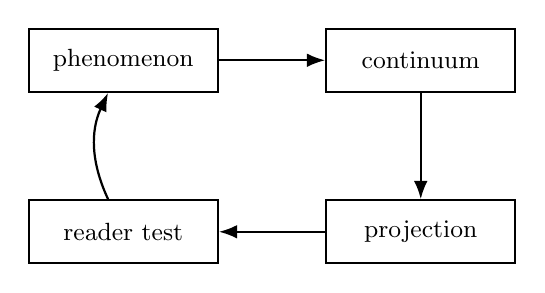
\begin{tikzpicture}[node distance=1.35cm,>=Latex,every node/.style={font=\small}]
\node[draw,thick,align=center,minimum width=2.4cm,minimum height=0.8cm] (a) {phenomenon};
\node[draw,thick,align=center,minimum width=2.4cm,minimum height=0.8cm,right=of a] (b) {continuum};
\node[draw,thick,align=center,minimum width=2.4cm,minimum height=0.8cm,below=of b] (c) {projection};
\node[draw,thick,align=center,minimum width=2.4cm,minimum height=0.8cm,left=of c] (d) {reader test};
\draw[->,thick] (a) -- (b);
\draw[->,thick] (b) -- (c);
\draw[->,thick] (c) -- (d);
\draw[->,thick,bend left=25] (d) to (a);
\end{tikzpicture}
\caption{Hierarchy Is Needed: concept map of conceptual dependency pressure 38-1-33}
\label{fig:figure-why-a-hierarchy-is-needed-one}
\end{figure}
The point of the diagram is not decoration; it marks which relation is being proposed and which stronger conclusion is still unavailable.\par
A local clarification is useful here\par
A local clarification is useful here\footnote{In Hierarchy Is Needed, this note clarifies the reader clarification role of the term and keeps the caveat close to the sentence that needs it.}.\par
The note keeps the caveat near the term without derailing the main sentence.\par
The point is not that every object must be surrounded by an elaborate diagram before anything can be said about it. A hierarchy is complete only relative to a question. If the question is whether the lake is safe for swimming today, a short chain of relevant descriptions may be enough: recent contamination, visible bloom, sampling history, weather, and local advisory. If the question is why the lake has changed over twenty years, the description must widen. It may need watershed land use, nutrient inflow, seasonal stratification, oxygen dynamics, species tolerance, measurement practice, and public intervention. The hierarchy grows only where the claim grows.\par
A crowded railway station during a delay makes the same need more immediate. The scene contains bodies, bags, doors, ticket barriers, platforms, announcements, phones, signs, and trains. It also contains expectations, missed connections, authority, frustration, trust, and decisions. A description that records only bodies in space can measure density, speed, pressure points, and congestion. That is not a bad description; crowd science and transport engineering depend on such measurements. But it cannot by itself explain why a clearer announcement, the opening of a side gate, or the sudden rumor that another train is leaving from a different platform can reorganize the crowd. The relevant event is not just matter moving through corridors. It is a coupled arrangement of bodies, signals, constraints, and expectations.\par
A purely psychological description would also fail if it forgot walls, platform widths, doors, staircases, and line-of-sight. Passengers may intend to move calmly, but a narrow staircase can turn calm intention into compression. They may want reliable information, but a broken sign can make rumor more powerful than official instruction. They may be rational, frightened, hurried, or resigned, and still be shaped by the architecture that permits some movements and blocks others. The station does not divide cleanly into matter on one side and mind on the other. Its behavior depends on relations among physical occupancy, information, institutional rules, and individual action.\par
A level is justified when such relations would be lost without it. At one level, the relevant units are bodies and obstacles; the relations are distance, flow, contact, blockage, and available routes. At another level, the units are passengers with destinations, tickets, habits, and obligations; the relations are priority, expectation, shared route, confidence, and response to authority. These levels overlap in one event, but they are not duplicates. A change in the wording of an announcement can change passenger behavior without moving a wall. A change in corridor width can change behavior without changing anyone's destination. Each level preserves a relation the other cannot carry alone.\par
William Wimsatt's work on reduction and levels is useful here because it treats levels as part of the practical labor of understanding complex systems, not as decorative vocabulary. A lower-level account may be indispensable and still not answer a higher-level question. A higher-level account may be useful and still depend on lower-level constraints. This double pressure is the important lesson. Hierarchy is not a refusal of reduction, and it is not a license for vague holism. It is a discipline for saying what kind of description is being used and what kind of relation it can preserve.\par
The lake and the station also show why boundaries matter. A boundary is not merely a line drawn around an object. It is a condition under which a difference matters. The edge of a queue, the skin of an organism, the perimeter of a jurisdiction, the interface of a software system, and the threshold of a sensor are not the same kind of thing. Yet each marks a place where some changes pass, some are blocked, and some are transformed. If a description has no way to say which boundary is active, it may confuse movement across a boundary with change inside a level.\par
Heat crossing into a lake, a passenger crossing through a gate, a rule crossing into enforcement, and a message crossing an interface are not interchangeable events. They can be compared only in a limited structural sense: in each case something changes under boundary conditions. That does not make ecology, crowd behavior, law, and software the same science. The comparison is descriptive before it is theoretical. It asks whether a relation has the same formal role in an explanation, not whether the domains are made of the same stuff or governed by the same mechanisms.\par
\section{The K-Level Reading In Hierarchy Is Needed}
Once levels are admitted, transformation must be handled carefully. A repeatable change under stated conditions can be called an operator: heating a lake, opening an exit, issuing a command, changing an incentive, adding a predator, altering a legal definition, or introducing a new measuring instrument. But no such operator is level-free. Heat changes molecular motion, water density, seasonal stratification, dissolved oxygen, microbial activity, fish behavior, and institutional risk assessment in different ways. If all of these are compressed into the sentence ``the lake got warmer,'' a useful shorthand becomes an obstacle to understanding. \cite{dakos_early_warning,parfit_reasons_persons}\par
The same problem appears in the station. Opening a side gate is a physical alteration of a route. It is also an informational event, because passengers notice that a path has become available. It may be an institutional event, because only authorized staff can open it. It may become a trust event, because passengers infer that the station is being managed competently or badly. One operator therefore has several effects, but those effects should not be merged into a vague claim that everything affects everything. Hierarchy keeps the effects apart long enough for their relations to be named.\par
The local dependency can now be written without changing the claim it supports.\par
\begin{equation}\label{eq:equation-why-a-hierarchy-is-needed-two}
\operatorname{boundaryResidual}_{9} = C_{\mathrm{unres}}=\min_{\pi\in\Pi}\|B(x)-B(\pi x)\|
\end{equation}
The relation names a local dependency, variable dictionary, and proof/evidence role; it is not a claim-status upgrade.\par
The formula is a restraint on the prose. It names the dependency that the surrounding paragraph is allowed to use.\par
The comparison below gives hierarchy is needed a set of quantities that can be inspected instead of merely admired.\par
\begin{table}[htbp]
\centering\small
\caption{Hierarchy Is Needed: observable quantities and counter-pressure 38-2-33}
\label{tab:table-why-a-hierarchy-is-needed-one}
\begin{tabular}{@{}llll@{}}
\toprule
Falsifier & Trigger & Expected failure & Consequence \\
\midrule
hierarchy is needed boundary & 21 units & declared case & fixes what is compared \\
residual pressure & 0.49 & dimensionless & shows unresolved load \\
projection loss & 0.77 & bounded interval & marks lost structure \\
countercase set & 12 cases & review sample & keeps a falsifier visible \\
\bottomrule
\end{tabular}
\end{table}
The table should be read locally: it narrows the comparison without pretending that the wider theory has been settled by a single surface.\par
Peter Olver's work on Lie groups belongs to a far more formal mathematical setting, but it clarifies a general pressure in the background. Transformations are not understood merely by listing changes one after another. They are understood by asking what is allowed to vary and what remains structurally recognizable through the variation. The lesson should not be inflated into a ready-made mathematics for lakes, crowds, institutions, or theories. Its value here is more restrained: whenever change is described, the description must say what kind of change it is and what identity is being preserved while it occurs.\par
That restraint matters because continua differ. A continuum is a dimension along which a system can vary while still being described as the same system. Temperature, crowd density, institutional trust, ecological diversity, explanatory precision, and legal recognition are not measurements on one master ruler. A hierarchy allows several continua to be used without pretending they can always be translated into a single quantity.\par
A system may be continuous at one level and discontinuous at another. The station may fill gradually, person by person, while a corridor becomes functionally blocked in a sudden way. The lake may warm gradually, while oxygen loss crosses a threshold at which a species can no longer survive. A scientific dispute may accumulate small objections for years, then reorganize around one distinction that changes what counts as a valid explanation. Gradual change in one continuum can become abrupt change in another.\par
This is why a single scale is tempting but dangerous. Complexity, information, efficiency, power, entropy, value, and adaptation can each illuminate a system within a defined model. None should be allowed to swallow all others without argument. A highly efficient system may be brittle. A stable system may be oppressive. A flexible system may be incoherent. A complex system may be poorly adapted to the question being asked of it. Hierarchy protects plural variation from premature conversion into one master measure.\par
Contradiction adds another pressure. In this account, contradiction is not only a formal logical error. It is also a conflict among descriptions, constraints, or operations that cannot all remain active in the same form. A city wants faster traffic and safer streets. A research program wants broad generality and strict measurement. An organism must conserve energy and respond quickly. A legal order wants predictable rules and equitable exceptions. Such conflicts may not be solved by choosing one sentence and discarding the other. They may require a new distinction, a new level, a narrower claim, or a recognition that the configuration has failed.\par
The word ``contradiction'' must be used with care across domains. A contradiction in formal logic is not the same thing as a conflict in urban planning, a tradeoff in physiology, or a tension in law. The analogy is structural, not identical. In each case, the description encounters demands that cannot all be satisfied in the same terms. The stronger theoretical claim begins only when the units, relations, boundaries, and transformations of the case have been specified. Without that discipline, cross-domain vocabulary becomes only resemblance.\par
Hierarchy therefore has an ethical as well as analytical function in prose. It slows down claims that want to move too quickly. A claim about molecules, a claim about organisms, a claim about institutions, and a claim about formal description do not carry the same evidence or the same risk. They may be connected, but connection is not identity. The hierarchy gives a way to say where a claim lives, what it can touch, and what it cannot silently absorb.\par
\section{Completeness Pressure In Hierarchy Is Needed}
Because levels are useful, they are also easy to invent too freely. A hierarchy becomes decorative when every topic is given its own shelf. ``Economy,'' ``mind,'' ``culture,'' ``technology,'' and ``biology'' name large areas of concern, but they do not automatically supply levels of analysis. A level earns its place only when it supplies a distinct unit of description, a distinct relation among those units, and a distinct pattern of transformation that cannot be recovered without loss from neighboring descriptions alone. \cite{dakos_early_warning,parfit_reasons_persons}\par
This criterion is operational rather than ornamental. It asks what is being counted, what connects the counted items, what counts as change, and under what boundary conditions that change matters. In the station, bodies can be counted one way and passengers another. A body occupies space and moves through a corridor. A passenger holds a ticket, hears an announcement, has a destination, and may decide to wait, reroute, leave, complain, or follow a crowd. The body and the passenger are not two separate beings. They are two ways of describing one person under different relations.\par
The local dependency can now be written without changing the claim it supports.\par
\begin{equation}\label{eq:equation-why-a-hierarchy-is-needed-one}
\operatorname{axisInformation}_{9} = \Delta d=\operatorname{rank}(A_{\mathrm{new}})-\operatorname{rank}(A_{\mathrm{old}})
\end{equation}
The relation names a local dependency, variable dictionary, and proof/evidence role; it is not a claim-status upgrade.\par
The formula is a restraint on the prose. It names the dependency that the surrounding paragraph is allowed to use.\par
The local dependency can now be written without changing the claim it supports.\par
\begin{equation}\label{eq:equation-why-a-hierarchy-is-needed-three}
\operatorname{projectionLoss}_{9} = P_{\mathrm{collapse}}=\sigma(\alpha R-\beta S-\gamma M)
\end{equation}
The relation names a local dependency, variable dictionary, and proof/evidence role; it is not a claim-status upgrade.\par
The formula is a restraint on the prose. It names the dependency that the surrounding paragraph is allowed to use.\par
A small numerical test keeps the abstraction honest at the scale of a single decision.\par
\paragraph{Numerical example.} For hierarchy is needed, take support=0.46, projection loss=0., and 1 open obligations. The bounded score is 0.200; the example gives the reader a numeric scale without pretending to be empirical proof.\par
The numbers are deliberately small; their value is pedagogical, not evidential, unless the chapter binds them to a dataset elsewhere.\par
The criterion rejects over-reduction. A crowd is not merely a gas of bodies, even though bodies still occupy space. An institution is not merely a building, even though it needs rooms, records, tools, and people. A theory is not merely ink or pixels, even though it must be expressed in marks or symbols that can be read, checked, and disputed. Lower-level description is often necessary. It is not always sufficient.\par
The criterion also rejects over-projection. A higher-level pattern cannot float free of its conditions. A law cannot act without offices, documents, procedures, recognition, and enforcement. A market cannot move without material channels, information, expectations, rules, and participants. A melody cannot be heard without sound or notation arranged in time. Higher-level description is often indispensable. It is not exempt from support.\par
A biological example makes this clearer when it is made specific. Consider a disturbance in heart rhythm. At one level, the relevant description may involve the organ: the heart as a pump coordinating contraction to move blood. At another, it may involve tissue conduction: electrical signals passing through pathways that synchronize muscular action. At another, it may involve cells: membrane potentials, ion channels, and local excitability. At another, it may involve genes or drugs that alter those channels. At another, it may involve the organism under stress, dehydration, infection, or exertion. An intervention that works at one level can fail or become dangerous if interpreted only at another.\par
A medication that changes ion-channel behavior is not adequately understood if it is described only as a molecular interaction. Its significance depends on tissue rhythm, organ function, patient condition, dose, monitoring, and risk. Conversely, saying ``the heart is not pumping properly'' may be clinically meaningful but mechanistically thin. The hierarchy is needed because the organism is not exhausted by any single level, and because intervention requires translation across levels without pretending that translation is automatic.\par
Here the comparison across domains must remain limited. A heart, a station, a lake, a bridge, and a legal institution do not share one hidden essence. They can be compared only by asking whether each case requires ordered descriptions of units, relations, boundaries, and transformations. In biology this may support empirical and mechanistic claims. In social or legal examples it may support descriptive or operational distinctions. In philosophical argument it may clarify conceptual burden. The hierarchy does not turn all these into the same kind of proof.\par
This criterion does not promise that every mapping between levels is already known. It is a rule for honest placement. If a lower-level mechanism is said to explain a higher-level pattern, the relation must be named. If a higher-level constraint is said to shape lower-level behavior, the constraint must be specified. If neither can be done, the claim remains provisional. The hierarchy does not hide the missing relation; it locates it.\par
A level is therefore justified when its removal would cause real descriptive loss. If removing it changes nothing, it was decorative. If removing it forces distinct relations into one confused vocabulary, it is needed. The hierarchy earns its keep when it preserves differences that the argument later depends on.\par
\section{A Rival Partition Test In Hierarchy Is Needed}
A new danger appears as soon as several levels are arranged. The diagram may look complete simply because it has several layers. But completeness cannot mean that every fact about a system has been captured. That standard would make explanation impossible. Completeness means that the description has included the levels required for the claim it is making. A hierarchy is complete only relative to a question. \cite{dakos_early_warning,parfit_reasons_persons}\par
Return again to the lake, because the example grows rather than repeats. A summer visitor asks whether the water is safe. A fisheries biologist asks why a species is disappearing. A town council asks whether runoff restrictions are necessary. A limnologist asks whether the lake is nearing a regime shift. These questions overlap, but they do not require the same hierarchy. The visitor may need recent sampling and visible signs. The biologist may need oxygen profiles, spawning conditions, food webs, and temperature tolerance. The council may need land use, agricultural practice, enforcement capacity, cost, and public compliance. The limnologist may need long-term variance, recovery rates, feedbacks, and early warning indicators.\par
The case that follows turns the proposal into a sequence of criticizable moves.\par
\paragraph{Worked case.} In the worked case for hierarchy is needed, the claim is reduced to a boundary, an observable, a dependency, a numerical cue, and a falsifier. The case is useful only because each move can be criticized separately.\par
The case helps because each step can fail separately, which is exactly what a useful example should permit.\par
Work by Dakos and colleagues on early warning signals for critical transitions matters here because it shows how patterns of change can precede abrupt shifts in some dynamical systems. Slower recovery from disturbance, rising variance, or changing autocorrelation may indicate that a system is approaching a threshold. But this work should not be treated as a universal alarm bell. It does not mean every lake, market, institution, or theory will politely announce collapse in the same way. Its relevance is more precise: when the question concerns transition, the hierarchy must include temporal dynamics and indicators appropriate to the system being studied.\par
Completeness pressure begins when a claim reaches beyond the levels it has described. ``The lake died because the water got warmer'' may be partly true, but it is too compressed for serious explanation. Warmer water holds less dissolved oxygen, alters density relations, affects seasonal mixing, changes microbial activity, interacts with nutrient load, and stresses species unevenly. The sentence may be acceptable in ordinary speech. It is not adequate when the explanation needs to distinguish mechanism, boundary, threshold, and intervention.\par
The station has its own version of this pressure. ``The crowd panicked'' may name something visible, but it can conceal many different structures: blocked exits, false information, authority failure, threat, density, confusion, or rational movement away from danger. If the sentence is accepted without hierarchy, it becomes impossible to know what changed the event. Was the decisive operator architecture, information, trust, danger, or crowd density? The description must open the levels required by the claim before the claim can be used.\par
This pressure does not demand endless expansion. The point is not to include everything. A description of a locked door does not need molecular metallurgy unless the lock fails because of material fatigue. A description of a legal border does not need individual psychology unless recognition, compliance, evasion, or fear is part of the phenomenon. A description of a theorem does not need the author's biography unless the claim concerns discovery, interpretation, reception, or error. The test is whether leaving a level out changes the meaning or adequacy of the claim.\par
Parfit's Reasons and Persons offers a philosophical comparison from a different territory. Parfit presses ordinary concepts of personal identity until they fail to settle cases involving bodily continuity, psychological continuity, division, and survival. The importance here is not to import his conclusions about persons into a general systems theory. It is to notice the pressure his method exposes: familiar vocabulary may work in ordinary cases and fail when a problem requires distinctions it does not contain. When that happens, one must either add a distinction, narrow the claim, or admit that the old description cannot decide the case.\par
Completeness pressure is strongest when two warranted descriptions cannot remain unchanged together. A city may be described as improving mobility by adding road capacity and as worsening mobility by inducing more traffic over time. The contradiction is not resolved by choosing the more convenient sentence. It may require levels of individual travel time, network flow, land use, induced demand, environmental cost, and public objective. The hierarchy does not solve the policy problem. It shows what kind of solution would count as honest.\par
A hierarchy therefore prevents premature closure. It asks, for each claim: what level has been left out, and does leaving it out change the claim? If the answer is no, the description can remain spare. If the answer is yes, the missing level is not optional complexity. It is part of the claim's meaning.\par
\section{What The Level Adds In Hierarchy Is Needed}
The movement toward hierarchy also passes through general systems thinking. Ludwig von Bertalanffy argued that many scientific problems require attention to organized wholes rather than isolated parts. His point was not that specialized sciences should be dissolved into a single vocabulary. It was that decomposition alone is not always enough. Organisms, societies, and other organized systems often display relations that appear only when parts are arranged, maintained, and transformed within a whole. \cite{dakos_early_warning,parfit_reasons_persons}\par
The important inheritance is a problem, not a completed solution. How can one speak across domains without pretending that all domains are the same? A lake, a crowd, a body, a bridge, a legal institution, and a formal theory are not interchangeable. They differ in material, evidence, method, and consequence. Yet each may involve boundaries, transformations, persistence, conflict, and failure. A hierarchy allows comparison at the level of descriptive structure while preserving differences in domain, evidence, and mechanism.\par
This is why systems language must be handled more strictly than it often is. It is easy to say that everything is connected. It is harder, and more useful, to say which units are connected, by what relation, across which boundary, under what transformation, and with what evidence. Without those questions, systems thinking becomes a style of association. With them, it becomes a discipline of organized description.\par
An organism shows the pressure clearly. The whole constrains the parts, and the parts sustain the whole. Cellular processes occur within tissues, organs, organisms, and environments. Disease may begin at one level and become intelligible only through another. A mutation may not matter in isolation, may matter in a tissue context, may matter under environmental stress, and may matter socially once diagnosis, access to treatment, and institutional decision enter the case. The point is not to make biology into sociology or sociology into biology. The point is to prevent one level from pretending to be the whole account.\par
Engineered systems show a related structure. A bridge has material properties, geometric design, load distribution, maintenance history, inspection regimes, weather exposure, traffic demand, and public use. A crack is a physical feature, but its significance depends on stress, redundancy, monitoring, regulation, and acceptable risk. Calling the crack ``small'' is not enough. Small relative to material failure? Structural redundancy? Inspection threshold? Public safety? The hierarchy keeps these questions distinct without isolating them.\par
Emergence is one of the places where this discipline matters most. A pattern or capacity may become describable at one level because of relations among elements at another level, while not being captured by naming those elements separately. A traffic jam emerges from vehicles, roads, rules, reaction times, and constraints, but the jam is not located in one car. A melody emerges from notes ordered in time, but the melody is not one note. A legal institution emerges from documents, offices, persons, procedures, and recognition, but it is not reducible to paper alone.\par
Emergence does not mean magic. It means that relations are doing explanatory work. If the lower level is ignored, emergence becomes mystical. If the higher level is denied, emergence disappears into parts. Hierarchy allows both constraints to remain visible: the pattern depends on lower-level arrangements, and the pattern has a descriptive identity at the level where it operates.\par
Collapse is the paired case. A bridge collapses physically when structural relations fail. A crowd-control plan collapses operationally when movement, information, and authority no longer produce orderly flow. A theory collapses intellectually when its central distinctions can no longer carry the claims made through them. These are not the same event type. The comparison is not an empirical claim that bridges, crowds, and theories obey one law of ruin. It is a structural question: which level lost the relations required for persistence?\par
The systems route makes hierarchy necessary because organized systems are neither mere piles of parts nor detached wholes. They are arrangements in which relations matter. A responsible account must not claim a system-level property until the relevant level has been named, and it must not claim cross-level explanation until the relation between levels has been stated.\par
\section{Why Levels Are Needed In Hierarchy Is Needed hierarch}
If hierarchy is rejected, several alternatives remain. Each is useful for some tasks. Each fails when a claim must move across levels without erasing the differences that make the claim intelligible. \cite{dakos_early_warning,parfit_reasons_persons}\par
Flat reduction describes every phenomenon at the lowest available level. In many contexts this is powerful. Chemistry needs atoms and molecules. Neuroscience needs cells and signals. Engineering needs materials and forces. But flat reduction fails when the question concerns relations not visible at the chosen level. A sentence cannot be understood by listing ink molecules. A law cannot be understood by listing paper fibers. A queue cannot be understood by listing shoes. The lower level is real, but the relevant relation has been left out.\par
Flat holism makes the opposite mistake. It describes the whole and treats parts as secondary or distracting. This too has legitimate uses. A physician may need a patient-level view, a planner may need city-level data, and an ecologist may need ecosystem dynamics. But flat holism fails when the whole changes because of lower-level mechanisms. A fever may require cellular and infectious explanation. Congestion may depend on local bottlenecks. An ecological shift may depend on species interaction or nutrient flow. The whole is real, but the mechanism has been blurred.\par
Strict domain partition protects expertise by insisting that biology, physics, sociology, law, mathematics, and ethics each have their own language. That protection is important. Expert domains should not be dissolved into a general vocabulary that ignores method and evidence. Yet strict partition fails when systems actually cross domains. Climate risk joins atmospheric physics, ecology, infrastructure, economics, law, and public trust. Public health joins biology, behavior, logistics, institutions, and communication. Artificial intelligence joins computation, labor, law, cognition, measurement, and political economy. A theory that refuses all cross-domain structure cannot describe coupled problems.\par
Metaphorical transfer moves too quickly in the other direction. It borrows a word from one domain and applies it elsewhere: ecosystems of ideas, viral content, social metabolism, institutional DNA, cultural evolution. Such metaphors can be vivid and sometimes useful. They become dangerous when they carry conclusions without carrying mechanisms. Calling an idea ``viral'' does not by itself establish replication fidelity, transmission channels, host susceptibility, mutation, or selection. Calling an institution an ``organism'' does not establish metabolism, reproduction, or homeostasis. Hierarchy makes transferred language answerable to units, relations, boundaries, and transformations.\par
A single master continuum offers another escape. It tries to place all systems on one scale: complexity, order, entropy, information, power, utility, adaptation, or optimization. Such scales can be illuminating inside defined models. They fail when they absorb distinct questions into one number or one axis. A hierarchy keeps multiple dimensions available where the system demands them.\par
Narrative sequence is the last tempting substitute. A narrative tells what happened first, next, and after that. It is indispensable for history, causation, and explanation. But narrative alone can hide level changes. A company grows, reorganizes, fails, and is acquired. That sequence may involve capital flows, leadership decisions, product defects, labor relations, regulation, market timing, and customer trust. Without hierarchy, the story may be persuasive while remaining analytically vague. Narrative needs levels when each transformation belongs to a different kind of relation.\par
These alternatives show that hierarchy is not an aesthetic preference. It is a remedy for specific forms of loss. Flat reduction loses higher-level relations. Flat holism loses lower-level mechanisms. Strict partition loses coupled structure. Metaphorical transfer loses operational discipline. A master continuum loses plural variation. Narrative sequence loses level distinction.\par
Two objections remain serious. The first is that levels are chosen. A scientist, engineer, jurist, or philosopher may divide a system differently depending on purpose. This is true. But chosen does not mean arbitrary. A chosen level can preserve or erase relations. It can make transformations visible or hide them. It can answer the question or change it without admitting the change. The criterion is not whether a level is eternal, but whether it is adequate to the claim.\par
The second objection is that hierarchy may smuggle in authority. In ordinary language, hierarchy often means rank. That meaning has to be set aside. A higher level is not more important by default. A lower level is not more fundamental for every purpose. A cellular process can be decisive in one question; an institutional rule can be decisive in another. The level that matters is the one whose transformations change the answer.\par
This is why a hierarchy is needed. Not to decorate the argument, not to rank the world, and not to make every problem more complicated than it is. It is needed because some truths are lost when a system is forced onto a single plane. Parts matter, wholes matter, boundaries matter, transformations matter, and the relations among them matter. A disciplined hierarchy lets the description stay honest about where it is speaking, what it can explain, and what still has to be connected before the claim is complete.\par
\chapter{Bertalanffy and the Systems-Theory Pressure for Levels}
\section{Why Levels Are Needed In Bertalanffy Systems-Theory Pressure Levels}
A system is not made intelligible merely by naming its parts. A kettle, a city, a nervous system, and a legal institution can all be described by listing components, but the list does not yet say what kind of thing is being explained. The central difficulty is that the same material can be organized under different descriptions, and those descriptions do different work. A cup of water is a collection of molecules, a thermal body, a drink, a measured volume, and a boundary-bearing object in a kitchen practice. None of these descriptions is automatically false. The problem is knowing when a description belongs to a distinct level and when it is only a redescription of the same level. \cite{parfit_reasons_persons,wimsatt_reductionism_levels}\par
A level is a disciplined way of saying that some patterns become stable only when parts are organized under a relation that is not visible from the parts taken one by one. This is the point behind much systems-theoretic thinking: organization matters. Ludwig von Bertalanffy helped make that thought explicit by arguing that living and organized systems require concepts that are not exhausted by atomistic enumeration. The claim here is narrower and operational. OC needs levels because later claims about continua, boundaries, operators, emergence, and collapse would otherwise slide between descriptions without saying when a shift has occurred.\par
The next diagram slows the argument down just enough to show how bertalanffy systems-theory pressure levels is being organized.\par
\begin{figure}[htbp]
\centering
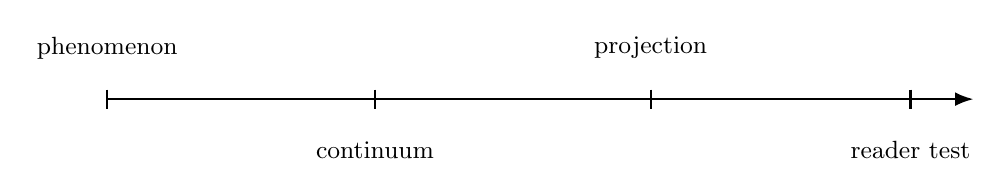
\begin{tikzpicture}[node distance=1.35cm,>=Latex,every node/.style={font=\small}]
\draw[->,thick] (0,0) -- (11,0);
\node[align=center] at (0,0.65) {phenomenon};
\node[align=center] at (3.4,-0.65) {continuum};
\node[align=center] at (6.9,0.65) {projection};
\node[align=center] at (10.2,-0.65) {reader test};
\foreach \x in {0,3.4,6.9,10.2} \draw[thick] (\x,0.12) -- (\x,-0.12);
\end{tikzpicture}
\caption{Bertalanffy Systems-Theory Pressure Levels: historical timeline of comparator test pressure 39-1-34}
\label{fig:figure-bertalanffy-and-the-systems-theory-pressure-for-levels-one}
\end{figure}
The point of the diagram is not decoration; it marks which relation is being proposed and which stronger conclusion is still unavailable.\par
A local clarification is useful here\par
A local clarification is useful here\footnote{In Bertalanffy Systems-Theory Pressure Levels, this note clarifies the reader clarification role of the term and keeps the caveat close to the sentence that needs it.}.\par
The note keeps the caveat near the term without derailing the main sentence.\par
Consider a traffic jam. At one level there are cars, engines, drivers, brakes, roads, and signals. At another level there is a wave of slowing that moves backward through traffic even while the cars move forward. The wave is not an extra vehicle hidden among the vehicles. It is a pattern of coordination and delay. A theory that only lists cars misses the wave; a theory that only speaks of traffic flow loses contact with the actions and constraints through which the flow is produced. The useful description has to keep both levels distinct without treating either as unreal.\par
This is why level language cannot be decorative. It prevents two opposite errors. The first error is flattening, where every phenomenon is forced downward into smaller parts before its organization has been described. The second error is inflation, where every interesting pattern is promoted into a separate reality without criteria. OC treats levels as necessary only when a description introduces stable variables, boundaries, or operators that cannot be replaced by a same-level inventory without losing the behavior under discussion.\par
The point is close to a warning in William Wimsatt's work on reduction and levels: complex systems often admit many partial reductions, but no single reduction automatically preserves all explanatory structure. A reduction may be useful for one purpose and destructive for another. In OC language, a reduction is acceptable only when the projection keeps the relevant continua and boundary conditions intact. When it does not, the level distinction has explanatory force.\par
\section{The K-Level Reading In Bertalanffy Systems-Theory Pressure Levels}
A level is introduced only when three conditions hold. First, there is a stable unit of description: something can be tracked across changes without dissolving into arbitrary detail. Second, there is a boundary condition: something marks what belongs to the described organization and what is treated as environment, input, output, or constraint. Third, there is an operator: some transformation acts on the described unit in a way that matters for the system's behavior. These terms are plain before they are technical. A stable unit is what remains identifiable. A boundary condition separates the treated system from what is not being treated as part of it. An operator is an action, rule, process, or transformation that changes the state of the unit. \cite{parfit_reasons_persons,wimsatt_reductionism_levels}\par
The traffic example makes the criterion concrete. A single car is a stable unit for mechanical and driver-level questions. A lane of traffic can also be a stable unit when the question concerns flow, density, and shock waves. The road edge, lane marking, speed limit, and signal pattern become boundary conditions. Acceleration, braking, merging, and signaling become operators. The traffic wave appears only when cars are placed in an organized relation. It is not explained by denying the car level, and it is not explained by pretending that the wave is independent of cars.\par
The local dependency can now be written without changing the claim it supports.\par
\begin{equation}\label{eq:equation-bertalanffy-and-the-systems-theory-pressure-for-levels-two}
\operatorname{collapseRisk}_{9} = \tau_{\mathrm{repair}}=\inf\{t:C(t)<\theta\}
\end{equation}
The relation names a local dependency, variable dictionary, and proof/evidence role; it is not a claim-status upgrade.\par
The formula is a restraint on the prose. It names the dependency that the surrounding paragraph is allowed to use.\par
The comparison below gives bertalanffy systems-theory pressure levels a set of quantities that can be inspected instead of merely admired.\par
\begin{table}[htbp]
\centering\small
\caption{Bertalanffy Systems-Theory Pressure Levels: observable quantities and counter-pressure 39-2-34}
\label{tab:table-bertalanffy-and-the-systems-theory-pressure-for-levels-one}
\begin{tabular}{@{}llll@{}}
\toprule
Level & Axis pressure & Operator burden & Transition test \\
\midrule
bertalanffy systems-theory pressure levels boundary & 24 units & declared case & fixes what is compared \\
residual pressure & 0.56 & dimensionless & shows unresolved load \\
projection loss & 0. & bounded interval & marks lost structure \\
countercase set & 13 cases & review sample & keeps a falsifier visible \\
\bottomrule
\end{tabular}
\end{table}
The table should be read locally: it narrows the comparison without pretending that the wider theory has been settled by a single surface.\par
The criterion also blocks loose talk. A mere size difference is not a level. A grain of sand, a pebble, and a boulder differ in scale, but scale alone does not prove a new level of explanation. A new level appears when the organization changes what can be tracked and transformed. A molecule in water, a droplet on glass, and a river in a valley are not just different sizes of wetness. They involve different boundaries, operators, and stable behaviors. Surface tension matters for the droplet. Channel geometry matters for the river. Molecular polarity matters for the chemical description.\par
This distinction matters because OC later uses hierarchy in a strict sense. A hierarchy is not a ranking of importance. It is an ordering of levels in which higher-level descriptions depend on lower-level conditions while introducing variables that are not interchangeable with those lower-level descriptions. The higher level is not magic; it is constrained. The lower level is not sovereign; it may be insufficient for the question being asked.\par
This also clarifies the scientific status of the proposal. The level criterion is a proposed operational discipline for description. It does not by itself prove that every later OC claim is true. It gives the reader a way to see what kind of burden later claims carry. When the book claims that a boundary, continuum, or operator belongs at a certain level, the claim has to show stable units, boundary conditions, and transformations at that level. Without those, the level is only a label.\par
\section{Completeness Pressure In Bertalanffy Systems-Theory Pressure Levels}
Once levels are admitted, a new demand appears. A theory cannot select levels only when they make an example convenient. If the same system can be described chemically, biologically, psychologically, and institutionally, the theory needs a way to say how those descriptions relate. This demand can be called completeness pressure. The phrase means the pressure on a framework to account for the levels needed by its own explanations, without pretending that every possible description is equally central. \cite{parfit_reasons_persons,wimsatt_reductionism_levels}\par
Completeness here does not mean total knowledge. It means that no essential level for the stated claim is silently omitted. A medical example is useful. A fever can be described as molecular signaling, immune response, whole-body temperature regulation, patient discomfort, clinical symptom, and public health datum. A molecular account alone may explain part of the mechanism. A clinical account alone may guide diagnosis. A public health account may track spread across a population. If an argument moves among these descriptions, it needs to preserve the level transitions instead of treating them as obvious.\par
The local dependency can now be written without changing the claim it supports.\par
\begin{equation}\label{eq:equation-bertalanffy-and-the-systems-theory-pressure-for-levels-one}
\operatorname{repairTime}_{9} = \operatorname{loss}_{\phi}=1-\frac{|E_{\phi}\cap E_{\mathrm{domain}}|}{|E_{\mathrm{domain}}|}
\end{equation}
The relation names a local dependency, variable dictionary, and proof/evidence role; it is not a claim-status upgrade.\par
The formula is a restraint on the prose. It names the dependency that the surrounding paragraph is allowed to use.\par
The local dependency can now be written without changing the claim it supports.\par
\begin{equation}\label{eq:equation-bertalanffy-and-the-systems-theory-pressure-for-levels-three}
\operatorname{replayCoverage}_{9} = I_{\mathrm{axis}}=\frac{\operatorname{Var}(x\mid a)}{\operatorname{Var}(x)}
\end{equation}
The relation names a local dependency, variable dictionary, and proof/evidence role; it is not a claim-status upgrade.\par
The formula is a restraint on the prose. It names the dependency that the surrounding paragraph is allowed to use.\par
A small numerical test keeps the abstraction honest at the scale of a single decision.\par
\paragraph{Numerical example.} For bertalanffy systems-theory pressure levels, take support=0.49, projection loss=0.11, and 2 open obligations. The bounded score is 0.127; the example gives the reader a numeric scale without pretending to be empirical proof.\par
The numbers are deliberately small; their value is pedagogical, not evidential, unless the chapter binds them to a dataset elsewhere.\par
The pressure becomes sharper when contradictions appear. In OC, a contradiction is not merely a verbal disagreement. It is an unresolved incompatibility inside a configuration of description or operation. A city may need more vehicles for mobility and fewer vehicles for breathable streets. A cell may need membrane closure for identity and membrane exchange for life. A person may need stable commitments and adaptive revision. These tensions cannot always be solved by choosing one side. Sometimes the system introduces a new dimension of description; sometimes the configuration breaks down.\par
Completeness pressure therefore asks whether the available levels can carry the contradiction. If a contradiction appears at the institutional level, a molecular description will not by itself settle it. If a contradiction appears in a biochemical pathway, a legal description will not by itself settle it. Each may constrain the other, but constraint is not replacement. The level at which the incompatibility is generated has to be identified before the possible resolution or collapse can be described.\par
This is where Anderson's essay More Is Different remains important. Anderson argued that the ability to reduce matter to lower-level laws does not eliminate the need for higher-level principles in organized phenomena. OC does not take that essay as a completed foundation. It uses the lesson more modestly: organization can generate stable explanatory questions at levels that are not erased by knowing the parts. Completeness pressure begins when a framework accepts that lesson and then has to specify which higher-level questions are actually present.\par
\section{A Rival Partition Test In Bertalanffy Systems-Theory Pressure Levels}
Bertalanffy's route into the problem begins with dissatisfaction toward explanations that treat organized beings as if they were only heaps of parts. General systems theory sought concepts for open systems, regulation, interaction, and organization across domains. The ambition was not merely to add new vocabulary. It was to name a structural problem: many phenomena persist by exchanging matter, energy, or information with their environments, and their order cannot be captured by a closed inventory of components. \cite{parfit_reasons_persons,wimsatt_reductionism_levels}\par
A living organism is the classic case. A body remains identifiable while its matter changes. It eats, breathes, repairs, excretes, adapts, and regulates. The material inventory is constantly changing, yet the organism remains a bounded organization for a time. This is not a denial of chemistry or physics. It is a claim about the kind of description needed. The organism has to be described as an open system, meaning a system whose persistence depends on exchange across its boundary.\par
The case that follows turns the proposal into a sequence of criticizable moves.\par
\paragraph{Worked case.} In the worked case for bertalanffy systems-theory pressure levels, the claim is reduced to a boundary, an observable, a dependency, a numerical cue, and a falsifier. The case is useful only because each move can be criticized separately.\par
The case helps because each step can fail separately, which is exactly what a useful example should permit.\par
OC inherits the pressure for such descriptions but narrows the method. It does not ask the reader to accept systems theory as a doctrine. It asks a more limited question: when an organized phenomenon persists through exchange, what level of description carries that persistence? The organism is not identical to a static list of molecules. It is also not an ungrounded vital force. It is a boundary-bearing, operator-governed continuity across change.\par
This route helps explain why the hierarchy of continua matters. A continuum is a range across which variation can be tracked: temperature, density, intensity, authority, permeability, commitment, attention, or any other ordered dimension that a domain can legitimately measure or describe. A hierarchy of continua is the arrangement of such ranges across levels. In the organism, chemical concentration, membrane permeability, tissue function, and behavioral adaptation are not the same continuum, yet they can constrain one another.\par
Bertalanffy supplies the historical pressure, not a finished OC apparatus. His systems theory makes it difficult to accept flat description as adequate for living and organized phenomena. OC then turns that pressure into a criterion: identify the level, name the continuum, state the boundary, specify the operator, and keep the claim within the status it has earned. This is the handoff from general systems intuition to operational metaontology.\par
\section{What The Level Adds In Bertalanffy Systems-Theory Pressure Levels}
The need for levels becomes clearer when alternative partitions fail. A partition is a way of dividing a phenomenon into units for description. Some partitions are useful. Others cut across the system in ways that destroy the behavior under study. If a mechanic divides a car into engine, transmission, wheels, fuel system, and electrical system, the partition fits many repair questions. If the same car is divided into all red parts, all warm parts, all metal parts, and all parts touched yesterday, the partition may be factual but explanatorily weak. \cite{parfit_reasons_persons,wimsatt_reductionism_levels}\par
The failure is not that the second partition is false. Some parts are red; some are warm; some are metal. The failure is that the partition does not preserve the operators relevant to the system. It does not show how force moves, how fuel becomes motion, how braking alters velocity, or how electrical failure stops ignition. A level criterion protects against this kind of factual irrelevance. Facts do not automatically become explanations.\par
The same point applies to social and conceptual systems. Derek Parfit's Reasons and Persons is useful here because it treats personal identity not as an untouchable primitive but as a problem of relations, continuity, and description. One need not accept all of Parfit's conclusions to learn from the method. If a person is partitioned only by body parts, the account misses memory, intention, responsibility, and psychological continuity. If a person is partitioned only by narrative, the account risks losing embodiment, vulnerability, and causal constraint. The explanatory level depends on the question and on the relations that preserve the phenomenon.\par
OC uses this lesson to avoid two temptations. It does not reduce every higher-level pattern to a lower-level inventory before asking what is being explained. It also does not license free-floating abstractions detached from conditions. The right partition is the one that keeps the relevant continuity and transformation visible. When no available partition does that, the theory faces a real problem rather than a stylistic inconvenience.\par
This is also why mathematical sophistication alone cannot rescue a bad level. A transformation group, as introduced in the study of Lie groups, describes structured transformations that preserve certain relations. Peter Olver's work on Lie groups and differential equations shows how powerful such transformation thinking can be in mathematics. But importing the prestige of transformation does not settle an OC claim. The relevant question is whether the transformation preserves the system features under discussion. A beautiful formal partition can still fail if it organizes the wrong invariants.\par
\section{Why Levels Are Needed In Bertalanffy Systems-Theory Pressure Levels routeS06}
The reader now has the minimum equipment needed for the later hierarchy claims. A level is not a mood, a metaphor, or a rank of importance. It is introduced when a stable unit, a boundary condition, and an operator appear together in a way that cannot be replaced by a same-level inventory without losing the behavior at issue. A hierarchy is an ordering of such levels, where dependence and novelty are both kept in view. \cite{parfit_reasons_persons,wimsatt_reductionism_levels}\par
The central example can be restated in one line. Cars make traffic possible, but a traffic wave is not a car. The wave requires cars, roads, drivers, spacing, reaction time, and constraint; nevertheless, the wave has a describable pattern of its own. A lower-level inventory supplies conditions. A higher-level description tracks organization. Scientific discipline lies in keeping both truths visible at once.\par
The Bertalanffy route matters because systems theory made this difficulty unavoidable for organisms and organized wholes. Open systems persist through exchange. They maintain identity across material change. They display regulation, breakdown, adaptation, and patterned relation to environment. These features force the language of level, boundary, operator, and continuum into view.\par
The objection is natural: perhaps levels are only conveniences in human description. OC can accept part of that objection. Levels are descriptions; they are not extra substances added to the world. But descriptions can be disciplined or careless. A disciplined level earns its place by preserving a behavior, relation, or transformation that the argument cannot otherwise state. Convenience becomes scientific only when the criteria are explicit.\par
The next step is to carry this discipline into the hierarchy of continua. Later claims can then be read with the right question in mind: what is the unit, what boundary makes it intelligible, what operator changes it, what continuum tracks the variation, and what level is actually doing the explanatory work?\par
\chapter{Criteria for a K-Level}
\section{Why Levels Are Needed In Criteria K-Level}
A system rarely presents all of its relevant structure at one descriptive height. A cup of water can be described as molecules in motion, as a fluid with viscosity and temperature, as a thermal reservoir in a laboratory procedure, or as part of a household routine in which someone waits for tea to cool. Each description can guide action and expectation. None is automatically the whole truth. The molecular description can explain why heat moves, but it does not by itself name the social fact that the tea is too hot to drink. The household description can explain why the cup is left untouched, but it does not replace thermodynamics. The same object is being handled through different descriptive levels. \cite{wimsatt_reductionism_levels,olver_lie_groups}\par
In the hierarchy of continua, shortened hereafter to OC, a level is a disciplined descriptive tier. It is not a decorative rank, a measure of importance, or a claim that higher descriptions are mystical additions to lower ones. A level exists when a system becomes intelligible through a stable set of objects, boundaries, relations, and operations that cannot be exchanged for another set without changing what is being explained. The word hierarchy names the ordering of such levels. It does not mean that every higher level commands every lower one. It means that descriptions can be arranged by dependence, scale, constraint, and transformation.\par
The next diagram slows the argument down just enough to show how criteria k-level is being organized.\par
\begin{figure}[htbp]
\centering
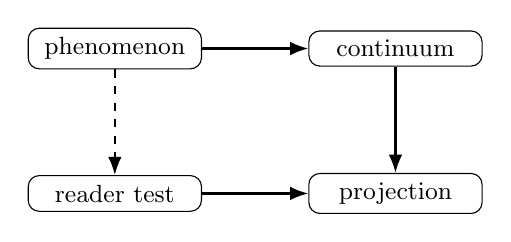
\begin{tikzpicture}[node distance=1.35cm,>=Latex,every node/.style={font=\small}]
\node[draw,rounded corners,align=center,minimum width=2.2cm] (a) {phenomenon};
\node[draw,rounded corners,align=center,minimum width=2.2cm,right=of a] (b) {continuum};
\node[draw,rounded corners,align=center,minimum width=2.2cm,below=of b] (c) {projection};
\node[draw,rounded corners,align=center,minimum width=2.2cm,left=of c] (d) {reader test};
\draw[->,thick] (a) -- (b);
\draw[->,thick] (b) -- (c);
\draw[->,thick] (d) -- (c);
\draw[->,thick,dashed] (a) -- (d);
\end{tikzpicture}
\caption{Criteria K-Level: dependency dag of domain projection pressure 40-1-35}
\label{fig:figure-criteria-for-a-k-level-one}
\end{figure}
The point of the diagram is not decoration; it marks which relation is being proposed and which stronger conclusion is still unavailable.\par
A local clarification is useful here\par
A local clarification is useful here\footnote{In Criteria K-Level, this note clarifies the reader clarification role of the term and keeps the caveat close to the sentence that needs it.}.\par
The note keeps the caveat near the term without derailing the main sentence.\par
The need for levels appears whenever a lower description is too crowded and a higher description is too vague. Consider a traffic jam. At one height, there are cars, drivers, braking distances, lane changes, and road geometry. At another height, there is a wave of congestion moving backward along a highway even though the cars themselves move forward. The wave is not a new substance floating above the cars. It is a pattern that becomes visible only when the description treats many vehicles together and tracks their collective relation over time. A driver feels the jam as stop-and-go motion; a traffic engineer may model the jam as a propagating disturbance. Both descriptions depend on vehicles, but the second introduces a level at which the jam has its own operational identity.\par
This is why OC needs a notation for levels rather than only the ordinary word level. Ordinary language uses level loosely. It can mean floor, rank, intensity, layer, maturity, or scale. A K level is more specific. The letter K marks a position in an ordered descriptive stack without pretending that the position is a moral rank or an ultimate layer of reality. It lets later claims say, in compact form, which tier of objects, boundaries, operators, and observables is being used. K is a bookkeeping device for disciplined comparison: not merely a tier, not merely a scale, but a named place in a hierarchy where claims must carry their own conditions of use.\par
A claim about a system has to say where it is being made. If a statement belongs to the molecular level, it cannot be dismissed merely because it does not mention household routines. If a statement belongs to the social level, it cannot be accepted merely because it borrows a physical metaphor. Level discipline protects inquiry from two opposite errors: reducing everything too early, and multiplying descriptions without criteria.\par
William Wimsatt's work on reductionism and levels is useful because it treats levels as tools for organized explanation rather than as slogans. His lesson, for this purpose, is that a level can be robust across several ways of looking while still depending on lower arrangements. OC borrows that balance. It does not borrow a license to declare every interesting pattern a real level. The question remains more demanding: what descriptive tier is required for a claim to be stated, checked, and limited without losing the phenomenon?\par
Systems also change their relevant vocabulary when they cross a boundary. A boundary is any condition that separates one regime of description from another: the edge of a cell membrane, the threshold at which a material cracks, the rule that turns private preference into a market price, or the institutional line that turns a conversation into a contract. Boundaries need not be walls. They can be thresholds, interfaces, constraints, conventions, or measurement conditions. What matters is that crossing them changes what counts as an object and what counts as an operation.\par
The traffic jam gives the change a concrete shape. Below a certain density, the important operations are acceleration, braking, and lane choice. Above a certain density, the same operations produce collective waves, bottlenecks, and synchronized motion. The cars have not ceased to be cars. The drivers have not ceased to make local decisions. Yet the description has changed because the system now displays patterns that are not naturally expressed by listing individual intentions. The point is not that the collective description has been empirically confirmed in every instance by naming it. The point is narrower and more useful: before later claims about emergence, contradiction, or collapse can be assessed, OC must show that the proposed level has a coherent descriptive role.\par
\section{The K-Level Reading In Criteria K-Level}
A K level is an operational level in the OC hierarchy. The letter K marks a place in an ordered stack of descriptive tiers, not a numerical promise of superiority. A K level is acceptable when four conditions hold together. It has identifiable objects. It has boundaries that determine when those objects are being described under that level. It has operators, meaning repeatable transformations or actions that change states within the level. It has observables, meaning features that can be inspected, measured, recorded, or otherwise constrained by experience at that level. \cite{wimsatt_reductionism_levels,olver_lie_groups}\par
The criterion can be stated plainly: a K level is warranted when its objects, boundaries, operators, and observables form a stable descriptive unit that explains, tracks, or organizes a phenomenon better than an unstructured mixture of neighboring vocabularies. The criterion is not a demonstration that the level is fundamental. It is not empirical confirmation of any particular model. It is a test of descriptive necessity. If removing the level leaves the phenomenon invisible, badly distorted, or expressible only through an impractical enumeration of lower details, then the level has earned provisional standing.\par
The local dependency can now be written without changing the claim it supports.\par
\begin{equation}\label{eq:equation-criteria-for-a-k-level-two}
\operatorname{claimSupport}_{9} = \rho_{\mathrm{replay}}=\frac{N_{\mathrm{matched}}}{N_{\mathrm{declared}}}
\end{equation}
The relation names a local dependency, variable dictionary, and proof/evidence role; it is not a claim-status upgrade.\par
The formula is a restraint on the prose. It names the dependency that the surrounding paragraph is allowed to use.\par
The comparison below gives criteria k-level a set of quantities that can be inspected instead of merely admired.\par
\begin{table}[htbp]
\centering\small
\caption{Criteria K-Level: observable quantities and counter-pressure 40-2-35}
\label{tab:table-criteria-for-a-k-level-one}
\begin{tabular}{@{}llll@{}}
\toprule
Example & Parameter & Value & What changes \\
\midrule
criteria k-level boundary & 27 units & declared case & fixes what is compared \\
residual pressure & 0.63 & dimensionless & shows unresolved load \\
projection loss & 0.12 & bounded interval & marks lost structure \\
countercase set & 14 cases & review sample & keeps a falsifier visible \\
\bottomrule
\end{tabular}
\end{table}
The table should be read locally: it narrows the comparison without pretending that the wider theory has been settled by a single surface.\par
The traffic jam supplies the first working example. At the vehicle level, the objects are cars and drivers. The relevant boundaries include lane markings, safe distances, speed limits, and the physical road. The operators include braking, accelerating, merging, and changing lanes. The observables include speed, position, spacing, and driver response. At the congestion-wave level, the object is no longer a single car but a pattern of collective slowing. The boundaries include road segments, density thresholds, bottlenecks, and time windows. The operators include wave propagation, dissipation, compression, and release. The observables include flow rate, average speed, queue length, and backward-moving shock waves.\par
The second description does not abolish the first. It reorganizes it. A congestion wave cannot exist without vehicles, but it is not naturally treated as one vehicle. It has a scale, persistence, and motion that belong to the collective pattern. This is the kind of case OC needs because later claims about hierarchy cannot rest on verbal elevation alone. A level must earn its place by doing explanatory work.\par
The criterion also blocks careless inflation. Not every named perspective is a K level. A person's irritation in traffic may be important for psychology, but irritation does not automatically define a traffic-system level. It would become part of a distinct level only if a stable set of objects, boundaries, operators, and observables were introduced: drivers as attention-limited agents, frustration thresholds, reaction-time changes, and measurable effects on braking or lane-change behavior. Without that operational structure, irritation remains a relevant factor, not a level.\par
The same discipline applies in the opposite direction. A molecular description of a car's engine is not always the correct lower level for a traffic jam. It may be true that engines consist of molecular processes, but the jam usually depends on vehicle motion, driver response, and road geometry. Choosing a lower level requires relevance, not mere ontological depth. A lower place in the hierarchy is not automatically more useful, more exact, or more scientific for every question.\par
A second example can be drawn from biology. Consider blood clotting after a cut. At one level, the objects include platelets, clotting proteins, damaged vessel walls, and chemical signals. The boundaries include the wound site, the vessel surface, blood flow conditions, and local biochemical thresholds. The operators include adhesion, activation, aggregation, enzymatic conversion, fibrin formation, and clot stabilization. The observables include platelet count, clotting time, fibrin structure, blood flow, and biochemical markers. At another level, the object is not a single molecule or cell but hemostasis: the organized process by which bleeding is stopped while circulation remains possible.\par
The hemostatic level cannot be replaced by naming one protein. It is also not detached from proteins and cells. It appears when cellular behavior, vessel geometry, flow, signaling, and material change belong to one operational description. If the description stays too low, the system becomes a list of reactions and components. If it rises too high, the word healing may conceal the difference between clot formation, inflammation, tissue repair, and scar formation. A K level becomes useful precisely where it holds the process at the height where its objects, boundaries, operators, and observables can be stated together.\par
Philip Anderson's argument in More Is Different clarifies the importance of this move. The lesson OC takes from Anderson is that large collections can exhibit organizing principles that are not well handled as mere verbal summaries of lower parts. The limit of the borrowing is equally important. Anderson does not give OC permission to treat every collective pattern as finally irreducible. OC uses the lesson cautiously: a proposed level must be judged by whether the phenomenon can be handled with stable operations and observables at that tier, while leaving open the further questions of measurement, model selection, simulation, and formal analysis.\par
\section{Completeness Pressure In Criteria K-Level}
Once a K level is proposed, it comes under completeness pressure. The phrase sounds technical, but the ordinary meaning is simple. A level cannot merely be named and then left hollow. It is pressed to show enough of its structure to support the claims made at that height. A level that names objects but gives no operators is incomplete. A level that gives operators but no observables is incomplete. A level that relies on boundaries but cannot say when those boundaries apply is incomplete. Completeness here does not mean final knowledge. It means enough operational specification to keep the level from functioning as a loose metaphor. \cite{wimsatt_reductionism_levels,olver_lie_groups}\par
The traffic example makes the pressure visible. Suppose someone says that a highway has a collective mood. The phrase may capture a lived impression, but it cannot yet carry a disciplined claim. What are the objects? Drivers, vehicles, groups, or road segments? What are the boundaries? A rush-hour window, a city corridor, a weather condition, a signaling system? What are the operators? Delayed braking, risky merging, honking, route switching? What are the observables? Accident frequency, average following distance, lane volatility, heart-rate data, or survey reports? Until these questions receive disciplined answers, the phrase may be evocative, but it is not yet a K level.\par
The local dependency can now be written without changing the claim it supports.\par
\begin{equation}\label{eq:equation-criteria-for-a-k-level-one}
\operatorname{domainError}_{9} = G=(V_{\mathrm{claim}}\cup V_{\mathrm{evidence}},E_{\mathrm{support}}\cup E_{\mathrm{challenge}})
\end{equation}
The relation names a local dependency, variable dictionary, and proof/evidence role; it is not a claim-status upgrade.\par
The formula is a restraint on the prose. It names the dependency that the surrounding paragraph is allowed to use.\par
The local dependency can now be written without changing the claim it supports.\par
\begin{equation}\label{eq:equation-criteria-for-a-k-level-three}
\operatorname{levelClosure}_{9} = \epsilon_{\mathrm{domain}}=\max_i |y_i-\hat y_i|
\end{equation}
The relation names a local dependency, variable dictionary, and proof/evidence role; it is not a claim-status upgrade.\par
The formula is a restraint on the prose. It names the dependency that the surrounding paragraph is allowed to use.\par
A small numerical test keeps the abstraction honest at the scale of a single decision.\par
\paragraph{Numerical example.} For criteria k-level, take support=0.52, projection loss=0.16, and 3 open obligations. The bounded score is 0.; the example gives the reader a numeric scale without pretending to be empirical proof.\par
The numbers are deliberately small; their value is pedagogical, not evidential, unless the chapter binds them to a dataset elsewhere.\par
The clotting example shows the same pressure in another domain. If someone says that the body knows how to seal itself, the sentence may be acceptable as ordinary speech, but it is not yet a level. The proposed level must identify the relevant objects, whether they are platelets, protein cascades, vessel surfaces, or wound regions. It must state its boundaries, such as the injured site, circulating blood, and the threshold between local clotting and dangerous systemic coagulation. It must name operators, such as activation, binding, amplification, and dissolution. It must name observables, such as clotting time, fibrin density, platelet activation markers, and restoration of flow. Only then does the phrase become a candidate for organized inquiry.\par
Completeness pressure matters because OC studies continua. A continuum is a range in which states vary without requiring every change to be a clean jump. Temperature, density, attention, trust, stiffness, blood viscosity, and institutional commitment can all be treated as continua when the domain permits graded change. A hierarchy of continua therefore cannot rely only on named boxes. It has to explain how a system moves within a level and when movement within a level creates pressure toward another level.\par
Percolation theory offers a useful analogy, especially as presented in Dietrich Stauffer's work on percolation. In a lattice, adding occupied sites may at first produce scattered local clusters. At a critical region, a connected path can span the system. The spanning cluster is not introduced by fiat. It appears when local connections cross a threshold that changes the system's large-scale behavior. OC borrows from this the attention to thresholds, connectivity, and system-wide organization. It does not borrow a universal formula for all domains. Traffic, clotting, institutions, and materials do not become percolation systems simply because they involve thresholds.\par
The analogy shows why completeness cannot be reduced to a list of parts. A pile of local facts may still miss the relation that organizes them. In the highway case, individual braking events matter, but the congestion wave depends on how those events connect across vehicles and time. In clotting, individual biochemical reactions matter, but hemostasis depends on how activation, flow, adhesion, and fibrin formation organize around an injury. In an institution, individual decisions matter, but a policy shift depends on how authority, record, incentive, and enforcement connect. A K level becomes compelling when it captures such organizing relations without pretending to float free from the lower arrangements that make them possible.\par
Completeness pressure also exposes overreach. If a proposed level cannot specify its observables, then claims at that level must remain tentative. If a proposed operator cannot be distinguished from a narrative label, then it cannot be used as if it were a measured transformation. If a boundary changes from paragraph to paragraph, the level is not stable enough to support later formal claims. This restraint is part of OC's status discipline. Conceptual warrant is not empirical validation. Modeling usefulness is not simulation success. Simulation success is not a theorem. A formal result, where available, does not automatically validate the assumptions that made it possible. Each status must be named separately.\par
A useful objection arises here. A skeptic may ask whether the criterion merely redescribes what scientists already do when they choose models. In one sense, yes. OC is not trying to replace ordinary modeling practice with exotic vocabulary. It is trying to make explicit a recurrent operation that becomes easy to hide: the movement from one descriptive tier to another. Scientists, engineers, and theorists often know locally which level they are using. Trouble begins when claims travel across domains or when one field borrows the prestige of another without carrying its constraints. The K-level criterion gives a public way to ask what has traveled and what has not.\par
\section{A Rival Partition Test In Criteria K-Level}
The route associated with Ludwig von Bertalanffy's general systems thinking enters as a historical and conceptual orientation. General systems theory sought patterns that recur across living organisms, machines, and organized wholes without reducing them all to one substance or one field. The attraction of that route is clear: many systems seem to share features such as boundary maintenance, feedback, organization, and transformation. The danger is also clear: cross-domain language can become too general to constrain anything. \cite{wimsatt_reductionism_levels,olver_lie_groups}\par
OC inherits the problem, not a finished solution. It asks how a system-language can be broad enough to compare domains while still narrow enough to reject bad comparisons. K levels are part of that answer. They prevent the word system from doing all the work. Before a system can be compared with another system, the relevant level has to be named. A cell, a supply chain, a legal institution, and a weather front may all be systems, but the objects, boundaries, operators, and observables are not interchangeable.\par
The case that follows turns the proposal into a sequence of criticizable moves.\par
\paragraph{Worked case.} In the worked case for criteria k-level, the claim is reduced to a boundary, an observable, a dependency, a numerical cue, and a falsifier. The case is useful only because each move can be criticized separately.\par
The case helps because each step can fail separately, which is exactly what a useful example should permit.\par
The traffic jam distinguishes useful generality from empty generality. It is fair to say that a jam has feedback: braking by one driver influences another driver, whose response influences the next. It is fair to say that the road imposes boundary conditions. It is fair to say that density changes the regime of collective motion. But it would be careless to infer that traffic, immune response, financial contagion, and political polarization all obey the same laws because they all involve feedback and thresholds. The K-level criterion demands a more patient comparison. What are the objects in each case? What counts as a boundary? Which operators are repeatable? Which observables constrain the claim?\par
The clotting example brings the same caution closer to life. Feedback is present there too. Activated clotting factors amplify further activation; vessel surfaces guide local response; flow can both deliver necessary components and threaten to wash them away. Yet this does not make clotting the same kind of system as traffic. The objects are different, the time scales are different, the operators are different, and the observables belong to another domain of practice. Bertalanffy's lesson is that organized wholes deserve comparison. The limit of the lesson is that comparison must not erase the local grammar of each whole.\par
Hierarchy becomes a form of intellectual hygiene. A hierarchy of levels allows comparison without flattening. One domain may have a level in which local interactions produce collective patterns. Another may have a level in which rules and records produce institutional states. A third may have a level in which material constraints produce phase behavior. The existence of a level in each domain does not mean the levels are identical. It means that each domain can be examined for the same kind of descriptive adequacy.\par
Sophus Lie's work on transformation groups, as treated in Peter Olver's account of Lie groups and differential equations, gives a mathematical example of why transformations matter. A transformation group studies operations that can be performed while preserving relevant structure. OC does not claim that every K-level operator is a Lie-group action. That would overstate the formal status. The borrowed lesson is modest: when a theory names a level, it must care about transformations that leave the level recognizable and transformations that move the system out of it. The limit is just as clear: many OC operators may be empirical, institutional, biological, or conceptual rather than mathematical symmetries.\par
In the traffic case, increasing speed within free flow may preserve the free-flow level. Increasing density beyond a threshold may alter the relevant description. In clotting, ordinary local activation may preserve a wound-sealing process, while runaway coagulation may move the system into a pathological regime. In a material, elastic deformation may preserve one regime, while fracture moves the system into another. In an institution, debate may preserve a deliberative level, while a signed decision may move the system into an enforceable administrative level. The operator is not merely an action. It is an action considered with respect to the level it preserves, modifies, or breaks.\par
The Bertalanffy route therefore becomes productive only when paired with level criteria. Without criteria, general systems language risks producing similarities too quickly. With criteria, it becomes a disciplined inquiry into which similarities survive operational comparison. OC's hierarchy is designed to hold that tension: broad enough to let domains speak to one another, strict enough to prevent a borrowed analogy from becoming a claim about the world without further work.\par
\section{What The Level Adds In Criteria K-Level}
A partition is a way of dividing a system for description. The most familiar partitions are by scale, by physical part, by function, or by academic discipline. Each can be useful. None is automatically adequate for a K hierarchy. The failure of alternative partitions matters because a level criterion earns its value only where simpler divisions are not enough. \cite{wimsatt_reductionism_levels,olver_lie_groups}\par
Partition by scale is the most tempting. Molecules are small, cells are larger, organs are larger still, organisms larger again, and societies larger than organisms. Many real hierarchies do track scale. Yet scale alone fails when the relevant level is defined by organization rather than size. A legal contract may be a few pages, while a warehouse may cover thousands of square meters. The contract can govern the warehouse despite being smaller. A software protocol may be tiny as text and vast in operational reach. A traffic wave may extend across kilometers, but its defining feature is not length alone; it is the collective propagation of constraint through vehicle interactions.\par
Partition by physical part also fails on its own. A car can be divided into engine, wheels, brakes, chassis, and sensors. That division is useful for repair. It does not by itself describe traffic flow. The jam is not located in one part of one car. It is distributed across relations among cars, drivers, road geometry, signals, and time. A level criterion therefore cannot be replaced by a parts list. It must identify the relations and operators through which the phenomenon holds together.\par
Partition by function is better but still insufficient. One might divide a highway system into transport, signaling, enforcement, and maintenance. That helps explain what the system is for. But function can blur the difference between a designed role and an observed regime. A road is built for transport, yet a jam is a transport failure that becomes a stable traffic phenomenon. The jam is not the intended function of the highway. It is an emergent regime within the system. Anderson's lesson about higher organization is relevant again: collective order may appear as a consequence of many interactions, not as the execution of a planned function.\par
Partition by discipline produces another failure. Physics may describe motion, psychology may describe attention, economics may describe incentives, and urban planning may describe infrastructure. These divisions reflect human institutions of knowledge. They do not always match the system's own organization. A K level can draw from several disciplines when the phenomenon demands it. In the traffic case, the congestion-wave level may use physical flow, driver response, road design, and signal timing. The level is not owned by one department. It is warranted by the operational unity of the phenomenon.\par
The strongest objection to K levels is that they may look like an extra vocabulary placed on top of ordinary practice. The answer is that the vocabulary is only justified where it prevents a recognizable failure. If scale, parts, function, or discipline already give a clean description for a claim, then no additional level language is needed. OC gains nothing by renaming ordinary distinctions. The K-level criterion matters when those ordinary partitions cut the phenomenon in the wrong place.\par
A bridge under load gives another concrete example. Scale partition gives atoms, grains, beams, joints, and the full bridge. Parts partition gives deck, cables, towers, bearings, and foundations. Function partition gives support, transfer, damping, and passage. Discipline partition gives materials science, structural engineering, weather analysis, and maintenance policy. A crack that begins locally and reorganizes the risk state of the whole bridge crosses these partitions. It is material, structural, temporal, and administrative. The relevant level may be a damage-propagation level in which the objects are defects and stress paths, the boundaries are load conditions and inspection regimes, the operators are growth, arrest, redistribution, and repair, and the observables are crack length, strain, vibration signatures, and load response.\par
This example shows why level criteria are not merely philosophical tidiness. If the crack is treated only as a microscopic defect, the system risk may be missed. If it is treated only as a bridge-level danger, the material mechanism may be blurred. If it is treated only as an administrative maintenance item, the physical dynamics may be flattened into a set of checks. A K level is warranted when it lets the claim meet the phenomenon at the right descriptive height.\par
The biological example sharpens the same point. Blood clotting cannot be partitioned adequately by size alone, because molecules, cells, tissue surfaces, and flow conditions all participate in the same process. It cannot be partitioned by physical part alone, because the relevant event is not confined to one component. It cannot be partitioned by function alone, because the same machinery that prevents bleeding can, in another regime, threaten circulation. It cannot be partitioned by discipline alone, because chemistry, cell biology, fluid dynamics, and clinical observation all constrain the description. The hemostatic K level is justified only if these elements form an operational unit rather than a convenient collection of topics.\par
Wimsatt's emphasis on levels and robustness helps clarify the point. A good level is not a private viewpoint. It remains recognizable across several investigative angles. The damage-propagation level may be approached through inspection, simulation, material testing, and structural monitoring. The hemostatic level may be approached through laboratory assays, microscopy, flow models, and clinical observation. Those approaches need not be identical, and their status must be stated honestly, but their convergence can make the level more than a name. Robustness does not make the level absolute. It makes it harder to dismiss as a linguistic convenience.\par
Alternative partition failure also protects against premature unification. A theory that wants to compare domains may be tempted to announce one master partition: micro and macro, part and whole, agent and structure, local and global. Such pairs are often useful, but they are too blunt for the full range of continua OC wants to describe. A crack, a traffic wave, a clotting process, a market panic, a cell signal, and a legal threshold do not all divide cleanly along the same pair. K levels allow comparison after the local descriptive work has been done, not before.\par
\section{Why Levels Are Needed In Criteria K-Level criteria}
The minimum understanding needed for later OC claims is now in place. A K level is a proposed descriptive tier in a hierarchy of continua. It is warranted when objects, boundaries, operators, and observables form a stable unit that makes a phenomenon tractable without erasing dependence on neighboring tiers. It is rejected, revised, or held in reserve when it lacks operational structure, when ordinary partitions already suffice, or when its claims outrun the evidence and formal work available. \cite{wimsatt_reductionism_levels,olver_lie_groups}\par
The traffic jam, blood clotting, and bridge crack examples carry the same lesson from different directions. In the traffic case, the higher pattern is not a ghostly addition to vehicles; it is a collective regime that becomes visible under the right objects and observables. In the clotting case, the process is not exhausted by one molecule, one cell, or one medical label; it is an organized transformation across biochemical, cellular, material, and flow conditions. In the bridge case, the relevant danger is not exhausted by a microscopic crack or by a whole-bridge label; it lies in a level where defect growth, stress redistribution, inspection, and load response belong together. In each case, the level is a practical achievement of description.\par
The intellectual references used along the way have limited jobs. Wimsatt helps keep levels robust but nonabsolute. Anderson helps show why collective organization may require its own descriptive tier without proving final irreducibility. Stauffer's percolation work helps illustrate thresholds and connectivity without turning every threshold into a percolation model. Bertalanffy helps frame cross-domain system comparison while warning, by the very breadth of the project, against empty generality. Lie and Olver help mark the importance of transformations while leaving most K-level operators outside the strict domain of transformation-group mathematics. Each reference lends a lesson; none supplies a shortcut.\par
The scientific status remains disciplined. The K-level criterion introduced here is conceptual and operational. It does not by itself prove the central OC hypothesis. It does not establish that a specific dataset supports a domain claim. It does not imply that a formal derivation has been supplied. It does not turn analogies from percolation, transformation groups, reduction debates, or general systems thinking into universal laws. Those materials help orient the criterion and show why the problem is real; they do not settle later claims in advance.\par
The central payoff is that later terms can now be handled without drifting. Emergence can be discussed as the appearance of stable organization at a level that was not visible under a neighboring description. Collapse can be discussed as the loss of the conditions that keep a level coherent. Contradiction can be discussed as an unresolved incompatibility among operators, boundaries, or observables within or across levels. Projection can be discussed as the movement of a claim from one domain or level into another under explicit constraints.\par
A K level, then, is not a metaphor for importance, not a name for scale, not a replacement for measurement, and not a promise that a theory has already been confirmed. It is a criterion-governed descriptive tier. It matters because OC will later make claims about movement, tension, failure, and transformation across continua. Those claims can only be as disciplined as the levels they use. Before OC can ask whether unresolved contradiction produces a new dimension of description or collapses a configuration, it must know what counts as a description, what counts as a level, and what counts as moving between levels. The K-level criterion supplies that footing: name the objects, state the boundaries, define the operators, identify the observables, and let the proposed level survive contact with the phenomenon it is meant to describe.\par
\chapter{Why These Levels and Not Another Partition}
\section{Why Levels Are Needed In These Levels Not Another}
A system is rarely exhausted by the scale at which it is first noticed. A glass of water can be described as a volume with a temperature, as a gathering of molecules, as a surface where liquid meets air, as a sample in a laboratory, or as an object being carried by a person across a room. None of these descriptions is automatically false. None is automatically sufficient. The trouble begins when a claim made in one description is allowed to pass into another without asking what has changed. A molecule does not have the temperature of the glass in the same sense that the glass has it. A sample bottle does not contain every property of the river from which it was filled. A rim that matters for evaporation may not be the boundary that matters for ownership, measurement, or control. Levels are needed because claims move too easily when no one asks where they belong. \cite{olver_lie_groups,anderson_more_is_different}\par
The point can be felt before it is named. If someone says the water is hot, the sentence sounds simple until the question becomes precise. Hot to the hand, hot by thermometer, hot relative to room temperature, hot enough to change a chemical reaction, hot enough to violate a storage rule: each answer selects a different setting in which the claim has meaning. The same glass sits before us, but the object of attention is not quite the same. Sometimes the object is the liquid as touched. Sometimes it is the measured volume. Sometimes it is a condition in an experiment. Sometimes it is a hazard in a workplace. A good description does not merely choose a word; it chooses the world in which that word can do work.\par
The next diagram slows the argument down just enough to show how these levels not another is being organized.\par
\begin{figure}[htbp]
\centering
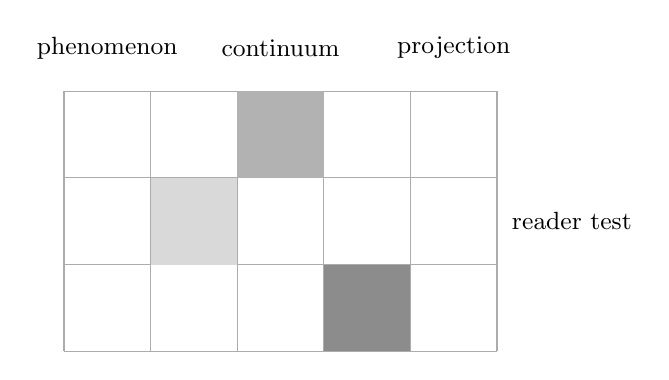
\begin{tikzpicture}[node distance=1.35cm,>=Latex,every node/.style={font=\small}]
\draw[step=1.1cm,gray!65,thin] (0,0) grid (5.5,3.3);
\node[align=center] at (0.55,3.85) {phenomenon};
\node[align=center] at (2.75,3.85) {continuum};
\node[align=center] at (4.95,3.85) {projection};
\node[align=center] at (6.45,1.65) {reader test};
\fill[black!15] (1.1,1.1) rectangle (2.2,2.2);
\fill[black!30] (2.2,2.2) rectangle (3.3,3.3);
\fill[black!45] (3.3,0) rectangle (4.4,1.1);
\end{tikzpicture}
\caption{These Levels Not Another: evidence matrix of conceptual dependency pressure 41-1-36}
\label{fig:figure-why-these-levels-and-not-another-partition-one}
\end{figure}
The point of the diagram is not decoration; it marks which relation is being proposed and which stronger conclusion is still unavailable.\par
A local clarification is useful here\par
A local clarification is useful here\footnote{In These Levels Not Another, this note clarifies the reader clarification role of the term and keeps the caveat close to the sentence that needs it.}.\par
The note keeps the caveat near the term without derailing the main sentence.\par
A level, in this sense, is not a decorative layer added to a diagram. It is a disciplined place of description, a range in which certain things can be picked out, certain changes can be followed, and certain boundaries matter. Later, this book will need more exact words for those parts of description. It will speak of continua: fields of variation that can be described without first reducing everything to isolated points. It will speak of operators: repeatable transformations or relations that change, preserve, combine, or carry a configuration. It will speak of projection: the rule-governed carrying of a description from one setting to another. But those words are useful only after the reader has seen the difficulty they answer. The difficulty is that the same situation can support several valid descriptions, and a sentence may become false or empty when moved to the wrong one.\par
Consider a fire in a room. At first it appears to be one event. Flame catches a curtain, smoke gathers near the ceiling, a detector sounds, someone hesitates at the doorway, and a corridor begins to fill. Yet the event is not one thing in the same way at every point of analysis. For the chemist, the fire is combustion: fuel, oxygen, heat, reaction rates, and the conditions under which the reaction sustains itself. For the engineer studying smoke, the fire is a source of hot gases moving through openings under pressure differences. For the person inside the room, it is a situation of perception and decision: smell, alarm, blocked sight, uncertainty, fear, and delay. For the architect or safety official, it is a test of compartments, sensors, doors, materials, routes, and codes.\par
Now imagine the sentence, the system failed. It may be true, but until the level is named it is too loose to guide thought. Did the chemistry fail to sustain flame, causing the fire to go out? Did ventilation fail, allowing smoke to accumulate where people needed visibility? Did the warning fail because the alarm was inaudible, ambiguous, or distrusted? Did the building fail by preserving the room while losing the corridor? Did human response fail because people searched for belongings before leaving? Each answer changes the subject of the claim. A room fire teaches level discipline because its causes and consequences do not sit in one vocabulary. Flame, smoke, design, and action are entangled, but they are not interchangeable.\par
This is not a demand to isolate descriptions from one another. In a real fire, combustion alters smoke; smoke alters human movement; human movement changes door states; door states change airflow; airflow returns to combustion. The point is almost the opposite. Because levels interact, they must first be distinguished. If they are not, the account mistakes contact for identity. The fact that a door changes smoke flow does not make a hinge a chemical reagent. The fact that panic alters evacuation time does not make panic a building material. The fact that a code required a sensor does not mean the sensor successfully communicated risk. Levels protect claims from being made with the wrong subject.\par
The same need appears whenever a system changes character. A pile of grains is not only many grains. Under pressure it can jam, flow, arch, avalanche, or bear load. A city is not only many people. It has traffic patterns, zoning constraints, institutions, bottlenecks, conventions, and infrastructures that shape what any person can do. A scientific community is not only many papers. It has training lineages, instruments, standards, citation habits, exclusions, incentives, and shared ways of deciding what counts as a result. The lower description matters; no serious account denies that. But the lower description alone may not supply the vocabulary needed for the higher pattern.\par
Philip Anderson's phrase, More is Different, has lasted because it names a recurring shock in scientific explanation. Many parts do not always make a larger copy of the part. Collective organization can bring new regularities into view, and with them new explanatory demands. The lesson is not that wholes float free of parts. It is that some properties are visible only at the level where the organization exists. Temperature is not found by looking for a tiny thermometer inside a molecule. Traffic flow is not found by naming one car. Trust in an institution is not found by weighing a document. The reality of dependence does not erase the need for the right description.\par
OC uses the name level for this disciplined place where description is stable enough to carry claims. A level is warranted when its objects, observables, boundaries, and transformations belong together. Objects are what the account can point to without immediately translating them away. Observables are what can be noticed, measured, compared, or tracked there. Boundaries are the constraints that decide what is inside, outside, admissible, exchanged, or excluded. Transformations are the repeatable changes or relations that make sense for those objects. In later chapters these transformations will often be called operators, but the ordinary word is enough for the first step: a level must have actions or relations that belong to it.\par
This vocabulary matters because the book will later consider a proposed OC hypothesis: unresolved contradictions sometimes force a system either to make a new dimension of description available or to lose the configuration that previously held. That is a conjectural rule of interpretation, not a proven law of nature, society, mathematics, and history. It is a disciplined way of asking what happens when an account cannot maintain its own conditions. To use it responsibly, one must first know where the contradiction appears, what counts as resolution there, and what would count as failure. A contradiction in an equation, a contradiction in bodily regulation, and a contradiction in a political institution are not the same object. They can be compared only when their levels have been named.\par
\section{The K-Level Reading In These Levels Not Another}
A useful partition cannot be chosen by taste. Familiar labels are tempting because they give the mind something to hold: physical, biological, psychological, social; micro, meso, macro; part, whole; theory, data. Each of these divisions can help in the right setting. None should be accepted merely because it looks orderly. A level earns its place when moving away from it changes what can validly be claimed. If nothing important is lost when the level is removed, the level was probably decorative. If removing it makes the claim ambiguous, false, or impossible to test in its own terms, the level was doing real work. \cite{olver_lie_groups,anderson_more_is_different}\par
The criterion begins with objects. At one level the object may be a molecule; at another, a cell; at another, a tissue; at another, an organism; at another, a population. These are not merely different sizes of the same word. A cell can be acted on, observed, and explained in ways that are not simply molecular sentences made longer. A tissue has organization that no isolated cell possesses. An organism has regulation, behavior, vulnerability, and history that are not exhausted by listing tissues. A population has distributions, transmission paths, reproduction rates, and ecological pressures. Each object is partly dependent on others, yet each can be the direct object of inquiry.\par
The local dependency can now be written without changing the claim it supports.\par
\begin{equation}\label{eq:equation-why-these-levels-and-not-another-partition-two}
\operatorname{simulationDrift}_{9} = \kappa_{K_9}=\frac{b_{K_9}+s_{K_9}}{1+o_{K_9}+q_{K_9}}
\end{equation}
The relation names a local dependency, variable dictionary, and proof/evidence role; it is not a claim-status upgrade.\par
The formula is a restraint on the prose. It names the dependency that the surrounding paragraph is allowed to use.\par
The comparison below gives these levels not another a set of quantities that can be inspected instead of merely admired.\par
\begin{table}[htbp]
\centering\small
\caption{These Levels Not Another: observable quantities and counter-pressure 41-2-36}
\label{tab:table-why-these-levels-and-not-another-partition-one}
\begin{tabular}{@{}llll@{}}
\toprule
Question & Observed cue & Local value & Reader use \\
\midrule
these levels not another boundary & 30 units & declared case & fixes what is compared \\
residual pressure & 0.70 & dimensionless & shows unresolved load \\
projection loss & 0.23 & bounded interval & marks lost structure \\
countercase set & 15 cases & review sample & keeps a falsifier visible \\
\bottomrule
\end{tabular}
\end{table}
The table should be read locally: it narrows the comparison without pretending that the wider theory has been settled by a single surface.\par
The second part of the criterion is the observable. An observable is something the description can notice and compare. At the molecular level, one may follow binding, concentration, charge, or reaction. At the cellular level, one may follow division, signaling, membrane potential, or differentiation. At the organismal level, one may follow symptom, movement, appetite, temperature, or pain. At the institutional level, one may follow compliance, authority, participation, trust, or failure of procedure. A proposed level without observables is only a name. It may sound impressive, but it gives the account nothing to see.\par
The third part is boundary. A boundary is not always a wall. It may be a membrane, a jurisdiction, a mathematical domain, a threshold of measurement, a membership rule, a protocol, a market edge, or a line beyond which a claim no longer applies. What matters is that the boundary constrains admissible states, exchanges, or interpretations. A cell membrane, a national border, a laboratory sampling rule, and the domain of a function are all boundaries in this broad sense, but they are not the same kind of boundary. Each belongs to a description in which certain crossings matter and others do not.\par
The fourth part is transformation. A level must have ways in which its objects change or relate while remaining intelligible as objects of that level. Diffusion, differentiation, voting, signaling, composition, evacuation, adjudication, circulation, and constraint propagation are not interchangeable verbs. They belong to different descriptions. In the more technical vocabulary of OC, such repeatable transformations or relations are called operators. The word should not make the idea mysterious. An operator is simply a rule-governed way something can be done to, with, or through the objects in view. What matters is that the transformation be meaningful at the level where it is used.\par
A level becomes suspect when one of these parts is missing. If it has objects but no distinctive observables, it may be a naming convention. If it has observables but no meaningful boundaries, it may be a loose field of variation rather than a level. If it has boundaries but no transformations, it may be a static classification. If it has transformations but no stable objects to receive them, it may be a metaphor pretending to be a method. The criterion is deliberately practical. It does not require every level to resemble physics. It requires each level to say what can be acted on, what can be observed, where distinctions hold, and which changes preserve or alter the configuration.\par
A mathematical analogy helps, if kept in its place. In the study of transformation groups, one learns a structure partly by asking what can be done to it without destroying the feature under study. Peter Olver's work on Lie groups and differential equations belongs to a precise mathematical tradition, not to a general metaphor about everything. Its usefulness here is not that every social, biological, or institutional system secretly is a Lie group. The useful discipline is the question: what remains meaningful under the transformations allowed here? A proposed level that cannot answer this question has not yet become operational.\par
The fire in the room now looks different. The combustion level has chemical species, temperature, oxygen supply, reaction rates, ignition, heat transfer, and extinction. The smoke-flow level has volumes, openings, pressure differences, buoyancy, visibility, deposition, circulation, and venting. The human-response level has persons, attention, trust, instruction, confusion, route choice, delay, search, and evacuation. The building-design level has compartments, stairs, doors, detectors, materials, signage, maintenance, and egress routing. These are not four arbitrary boxes placed over one event. Each level has objects, observables, boundaries, and transformations that make certain claims possible and make others invalid.\par
The difference becomes clearer if scale alone is used instead. Suppose investigators study the fire only by zooming in and out. At small scale they examine combustion. At larger scale they examine the room. At still larger scale they examine the building. But a tiny rule in the alarm protocol may govern hundreds of people, while a small door wedge may change smoke movement through an entire corridor. Scale notices size; it does not necessarily notice authority, meaning, function, or constraint. A sign no bigger than a hand can alter evacuation if people trust it. A microscopic failure in a sensor can change the institutional record of the event. A partition by size alone misses the level at which the relevant thing acts.\par
This is why hierarchy must not be heard as a fixed vertical ranking of reality. Higher does not mean better, truer, or more dignified. Lower does not mean more real for every purpose. A molecular account may be indispensable for mechanism, while an organismal account may be indispensable for symptom, and an institutional account may be indispensable for response. The hierarchy is a hierarchy of description. It is a way of asking which objects, observables, boundaries, and transformations belong together for the claim now being made. Its purpose is not to honor one level over another. Its purpose is to prevent two opposite mistakes: reducing a phenomenon until the relevant object disappears, and inflating a phenomenon until mechanism is lost.\par
\section{Completeness Pressure In These Levels Not Another}
Once a criterion for levels is in place, another problem appears. How many levels are enough? A partition with too few levels hides transitions that matter. A partition with too many levels creates artificial distinctions and makes every case look unique. The right number is not discovered by counting nature's shelves. It is discovered by pressure. A missing level announces itself when the account must smuggle in a distinction it has no place to put. \cite{olver_lie_groups,anderson_more_is_different}\par
Completeness here does not mean the final furniture of reality. It means coverage for the intended kind of claim. A map can be complete enough for navigation while useless for geology. It can be complete enough for property law while useless for bird migration. Taken literally, a perfectly complete map of a coastline would have to become the coastline. The useful map is complete relative to a purpose. In the same way, a hierarchy of levels is complete enough when it prevents the main category errors that would otherwise distort the claim being made.\par
The local dependency can now be written without changing the claim it supports.\par
\begin{equation}\label{eq:equation-why-these-levels-and-not-another-partition-one}
\operatorname{falsifierHit}_{9} = \operatorname{support}(c_{9})=P(c_{9})\wedge E(c_{9})\wedge R(c_{9})
\end{equation}
The relation names a local dependency, variable dictionary, and proof/evidence role; it is not a claim-status upgrade.\par
The formula is a restraint on the prose. It names the dependency that the surrounding paragraph is allowed to use.\par
The local dependency can now be written without changing the claim it supports.\par
\begin{equation}\label{eq:equation-why-these-levels-and-not-another-partition-three}
\operatorname{datasetSeparation}_{9} = \operatorname{falsify}(h)=\exists e\in E\,:\,\operatorname{pred}_h(e)\neq\operatorname{obs}(e)
\end{equation}
The relation names a local dependency, variable dictionary, and proof/evidence role; it is not a claim-status upgrade.\par
The formula is a restraint on the prose. It names the dependency that the surrounding paragraph is allowed to use.\par
A small numerical test keeps the abstraction honest at the scale of a single decision.\par
\paragraph{Numerical example.} For these levels not another, take support=0.55, projection loss=0., and 4 open obligations. The bounded score is 0.; the example gives the reader a numeric scale without pretending to be empirical proof.\par
The numbers are deliberately small; their value is pedagogical, not evidential, unless the chapter binds them to a dataset elsewhere.\par
A disease outbreak shows the pressure with unusual force. At first one may say that an outbreak is biological. That is true enough if the immediate task is to identify a pathogen, trace mutation, estimate incubation, or understand immunity. But the sentence becomes inadequate when transmission depends on housing density, labor conditions, transport routes, paid sick leave, trust in clinics, reporting practices, or the political cost of declaring danger. A virus does not move through a population as a pure biological abstraction. It moves through bodies that work, travel, gather, hide symptoms, seek care, avoid care, receive information, distrust information, and live under constraints.\par
The opposite reduction is just as dangerous. If the outbreak is described only as social, the account may capture inequality, communication, institutional trust, and coordination, but it will fail when dose, mutation, immunity, incubation, and treatment matter. A rumor can change behavior; it cannot by itself determine viral replication. A policy can slow contact; it cannot abolish biological latency by decree. A hospital system can reorganize beds; it cannot make a test reliable outside the conditions under which the test works. A useful hierarchy must keep biological, behavioral, infrastructural, and institutional descriptions available without melting them into a single vague story.\par
Imagine the first weeks of an outbreak in a city. A clinician notices an unusual cluster of symptoms. A laboratory confirms a pathogen. Several patients work in crowded kitchens and warehouses. Others share a bus route. A rumor spreads that reporting illness will cost workers their jobs. A health department issues guidance, but the guidance is written in language many residents cannot use. Employers interpret quarantine rules unevenly. Clinics lack staff for follow-up calls. The pathogen is biological, but the outbreak is not intelligible at the biological level alone. The social response is crucial, but it cannot be evaluated without the timing, transmissibility, and clinical course of the disease. The event forces a layered account because failure at one level changes what becomes possible at another.\par
The pressure toward completeness is therefore not the urge to include everything. It is the pressure exerted by missed transitions. When a new observable appears only after aggregation, when a boundary becomes active only under interaction, when a transformation changes type as it moves into another description, or when a contradiction cannot even be named at the present level, the partition is incomplete for that claim. The missing level is not added because the system is complicated. It is added because the current description cannot carry the distinction it is being asked to carry.\par
Percolation theory offers a disciplined encounter with this problem. In its classical mathematical setting, it studies how local connections can produce global connectivity. Dietrich Stauffer's introductions and Geoffrey Grimmett's more formal treatment show how a system may cross a threshold at which scattered local relations give rise to a spanning structure. The point for this chapter is narrow. Percolation is not a universal model of all emergence. It does not explain institutions, organisms, or meanings by magic. It teaches something more restrained and more valuable: a property may become describable only when the pattern of connection reaches the right condition. Inspecting one site in isolation cannot tell the whole story of global connectedness.\par
The lesson returns us to levels. If the hierarchy contains only individual sites, it misses the connected structure. If it contains only the global state, it misses the local conditions that make the state possible. The phenomenon demands both. A level is needed at which local connection is described, and another at which system-wide connectivity becomes an observable. The same general form appears outside mathematics, though without the same formal guarantees. A rumor becomes a public fact only after patterns of repetition and trust reach a certain condition. A supply chain failure becomes systemic only when local shortages connect through dependencies. A traffic slowdown becomes a jam when local braking and density produce a collective state.\par
The practical test is simple. Ask what would be lost if a proposed level were removed. If nothing changes except the wording, the level was decorative. If removal makes a claim ambiguous, invalid, or impossible to test in its own terms, the level is necessary for that claim. A hierarchy should be sparse enough that each level earns its place and rich enough that essential transitions do not have to be introduced through a side door. It should not multiply distinctions for elegance. It should admit them when the account breaks without them.\par
Two failures wait on either side. The first is flattening. Every system is described in one preferred vocabulary, and important differences are treated as surface variations. The second is fragmentation. Every domain receives its own private language, and comparison becomes impossible. OC tries to hold the middle. It allows different domains to keep their real differences while giving the analyst a way to ask parallel questions about variation, boundary, transformation, contradiction, emergence, and failure. The hierarchy is complete enough only when it lets those questions be asked without pretending that all systems are the same.\par
\section{A Rival Partition Test In These Levels Not Another}
The route to levels passes through general systems thinking, but it cannot stop there. Ludwig von Bertalanffy argued against studying organized phenomena only as isolated parts. Living systems, ecological arrangements, and institutions often have exchanges, feedbacks, relations, and forms of organization that cannot be understood by listing components alone. That inheritance matters. OC also begins from dissatisfaction with isolated-object description. A system is not merely a heap. It is a structured field of constraints, variations, and transformations. \cite{olver_lie_groups,anderson_more_is_different}\par
General systems theory gave permission to ask about organization across domains. That permission was historically important because it resisted the habit of treating every serious explanation as a descent into smaller pieces. But permission is not yet discipline. If words such as system, boundary, feedback, and level can mean anything in any setting, cross-domain comparison becomes a resemblance of language rather than an advance in thought. The task is to keep the ambition of systems thinking while tightening the terms under which comparison is allowed.\par
The case that follows turns the proposal into a sequence of criticizable moves.\par
\paragraph{Worked case.} In the worked case for these levels not another, the claim is reduced to a boundary, an observable, a dependency, a numerical cue, and a falsifier. The case is useful only because each move can be criticized separately.\par
The case helps because each step can fail separately, which is exactly what a useful example should permit.\par
This is where the hierarchy earns its place. It asks, for any description, what must be present for the description to work. What are its objects? What can it observe? Which boundaries matter? Which transformations are meaningful? What happens when the description is carried elsewhere? The last question introduces projection, one of the terms needed later in the book. A projection carries a description from one level, domain, or coordinate scheme into another under an explicit rule. Projection is not ordinary translation. It does not promise that everything survives. It may preserve some relations, discard others, distort others, or reveal that the attempted transfer is invalid.\par
A street map is a familiar projection. It carries terrain, buildings, names, roads, and distances into symbols useful for navigation. It gains power by losing detail. The texture of a wall, the smell of a bakery, the private history of an apartment, and the daily pattern of sunlight may disappear because they do not serve the map's rule. A medical risk score is another projection. It carries many biological and historical details into a smaller clinical decision surface. A legal category projects varied human circumstances into a form a court can process. In each case, the question is not whether the projection is complete in every sense. The question is what it preserves, what it loses, and whether the loss is lawful for the use at hand.\par
Claims that cross levels need the same discipline. If a cellular mechanism is projected into organism-level disease behavior, the account must identify how mechanism and symptom are related. It cannot merely say that one explains the other. If an institutional pattern is projected into a model of individual decision, the account must say what happens to norms, incentives, coercion, information, and habit. If a mathematical structure is projected into an empirical example, the account must say which features correspond and which do not. A projection without such discipline becomes an analogy that has forgotten its limits.\par
The route through Bertalanffy also clarifies why OC is not a reductionist program, though it respects lower-level mechanisms. Reduction is powerful when the target phenomenon can be reconstructed in the chosen lower vocabulary without losing what made it the target. Sometimes that is exactly what good explanation requires. But many systems demand an account of organization, boundary, and relation that is not visible in a mere inventory of parts. Anderson's argument about emergent regularities gives one scientific reason for caution: many-body systems can require concepts that appear at the level of collective organization. The broader descriptive rule is simple: do not erase the level at which the relevant observable exists.\par
Nor does this give permission to ignore mechanism. A higher-level claim can be empty if it cannot say how it is constrained by lower-level conditions, neighboring levels, or admissible projections. The point is not to choose between parts and wholes. It is to prevent a claim from borrowing authority from a level it has not earned. A hierarchy lets an account move downward toward mechanism, upward toward organization, and sideways toward analogy while keeping these movements distinct. Downward movement asks what makes the phenomenon possible. Upward movement asks what organization it enters. Sideways movement asks what structure is preserved when the description travels.\par
The fire example can be read through this route. A building code projects many past events, materials tests, engineering judgments, legal choices, and moral commitments into a rule about doors, alarms, exits, and compartments. The code is not the fire, and it is not merely a social opinion about fire. It is a projection from accumulated knowledge and institutional authority into design constraints. When a fire occurs, the code's level meets combustion, smoke, human response, and maintenance. If the door fails because it was propped open, the failure is not only physical and not only institutional. The hinge, the habit, the inspection regime, and the smoke path have to be described at their proper levels and then related.\par
The route through systems thought therefore leads to a stricter place than the word system alone suggests. Organized phenomena require relational description, but relational description must be controlled. OC adds level criteria, projection discipline, and explicit attention to emergence and failure. The result is not a proof that every later claim is correct. It is a vocabulary in which later claims can be stated without confusing the place where a phenomenon is generated, the place where it is observed, and the place where it is compared.\par
\section{What The Level Adds In These Levels Not Another}
A hierarchy earns trust partly by facing alternatives. The levels used here are not defended by saying that no other partition could ever be useful. Many partitions are useful for local purposes. A hospital may divide a case by department. A physicist may divide a problem by scale. A lawyer may divide a dispute by jurisdiction. A software engineer may divide a system by service boundaries. The question is narrower: which partition can carry claims about variation, boundaries, transformations, contradiction, emergence, failure, and projection without producing predictable category errors? \cite{olver_lie_groups,anderson_more_is_different}\par
One alternative is the part-whole partition. It divides the world into components and aggregates. This is often a good beginning because it asks what a thing is made of and how pieces combine. But it fails when the relevant difference is not part versus whole. A traffic jam is not merely a whole made of cars. It is a dynamic condition produced by density, reaction time, route constraint, signaling, driver expectation, weather, and local decisions. The part-whole partition can list vehicles, but it does not by itself supply the level at which flow failure becomes the object.\par
A second alternative is the micro-macro partition. This is sharper than part-whole because it recognizes scale. It distinguishes small interactions from large outcomes. Yet it remains too coarse. Many important descriptions sit between micro and macro, and some cross them. A cell is macro relative to molecules and micro relative to tissue. A household is macro relative to persons and micro relative to an economy. A local mathematical operation may impose a global constraint. If every case is forced into micro or macro, the partition hides intermediate levels where actual observables and transformations live.\par
A concrete failure shows the problem. Suppose a city's traffic authority studies congestion only as a micro-macro problem. At the micro end, it examines driver behavior. At the macro end, it measures citywide travel time. Both are valuable, but the missing level may be the intersection timing system, the bus lane rule, the bridge bottleneck, or the school dismissal schedule. These are not simply small or large. They are organized constraints that transform many individual choices into a collective pattern. Scale alone gives the wrong answer because the active object is neither the single driver nor the whole city. It is the regulated passage through a particular network condition.\par
A third alternative is the domain partition: physics, biology, psychology, society, mathematics, and so on. This is useful for expertise, methods, and literature. It fails as the primary hierarchy because domain boundaries do not always match level boundaries. Biology contains molecular, cellular, organismal, ecological, and evolutionary descriptions. Social analysis contains individual, group, institutional, infrastructural, and symbolic descriptions. Mathematics can describe structures that project into several domains without belonging to any one empirical scale. A domain partition tells us where a claim comes from; it does not automatically tell us at what level the claim is valid.\par
A fourth alternative is the data partition: what can be directly measured, what can be inferred, what can be simulated, and what remains theoretical. This partition is valuable for scientific discipline. It prevents a model from being mistaken for a measurement, or an inference from being mistaken for direct observation. But it cannot replace levels, because the same level may contain measurement, inference, simulation, and theory. Conversely, the same dataset may mix levels unless it is carefully constructed. Data status tells us how a claim is supported. Level tells us what kind of object the claim is about.\par
A fifth alternative is the narrative partition: origin, development, crisis, resolution. This can make a system intelligible over time, but it risks treating temporal sequence as explanatory structure. A crisis may occur at one level because a contradiction at another level has become unmanageable. A resolution may preserve one level while damaging another. An organization may solve a budget problem by destroying trust. A government may preserve a symbol while losing administrative capacity. A medical intervention may stabilize a number while worsening the patient's lived condition. Narrative gives sequence; it does not by itself distinguish which level changed and which level supplied the scene.\par
These alternatives are not mistakes in themselves. They become mistakes when used for a job they cannot do. Part-whole division is too static for transformations. Micro-macro division is too coarse for intermediate organization. Domain division is too tied to disciplines. Data division is about evidential status rather than descriptive object. Narrative division is temporal rather than operational. The hierarchy needed here must ask, at each stage, what kind of object is being described, what variation matters, what boundary is active, what transformations are allowed, what projection is being attempted, and what would count as emergence or collapse.\par
Collapse is another word that needs care. In ordinary speech it can mean breakdown, defeat, exhaustion, simplification, failure, or sudden loss of structure. In this book it should not be allowed to mean all of those things at once. A configuration collapses, in the relevant sense, when the arrangement that made certain objects, boundaries, or transformations coherent can no longer maintain them. That may be a mathematical inconsistency, a biological failure of regulation, an institutional loss of legitimacy, or a practical breakdown of coordination. The word becomes useful only when the level is named. Otherwise collapse is just a dramatic synonym for bad outcome.\par
The strongest objection is that any hierarchy can become a rigid grid. It can force phenomena into boxes and punish borderline cases. The answer is to make level membership conditional on use. A proposed level is not sacred. It must earn its place by carrying a stable combination of objects, observables, boundaries, and transformations. Borderline cases are not embarrassments; they are often where the work is. A virus, a legal person, a computer simulation, a climate model, and a mathematical idealization all strain ordinary partitions. The response is not to abandon levels, but to make the level assignment explicit and revisable under stated criteria.\par
Another objection is that levels may hide causal continuity. If organismal behavior depends on cellular processes, and cellular processes depend on molecular interactions, why not insist on one continuous account from bottom to top? The answer is that continuity of dependence is not identity of description. A bridge depends on steel microstructure, but traffic engineering is not replaced by metallurgy. A court decision depends on human bodies, paper, speech, and buildings, but legal validity is not replaced by chemistry. Dependence constrains higher-level claims. It does not automatically supply their vocabulary.\par
A final objection concerns emergence. The word can become lazy. A writer can call something emergent whenever the mechanism is unknown. That will not do. Emergence, in this setting, means that a new description becomes necessary because the relevant observable, boundary, or transformation is not available at the prior level in the same form. It is not a synonym for mystery. Percolation gives a disciplined example: system-wide connectivity appears under specific conditions of local connection, and the global state is not captured by inspecting one site alone. The lesson is not that every emergence is percolation. The lesson is that new level descriptions require conditions, not wonder.\par
\section{Why Levels Are Needed In These Levels Not Another levelsS0}
The hierarchy can now be read without treating it as a decorative stack. A level is a disciplined range of description in which certain objects, observables, boundaries, and transformations belong together. A continuum is a describable spread of variation. A boundary is a constraint on admissible states, exchanges, or interpretations. An operator is a repeatable transformation or relation. A projection carries a description across levels or domains under a rule that specifies what is preserved, lost, or changed. Collapse names the loss of a configuration only when the configuration and its level have been identified. These terms are not ornaments. They keep claims from traveling farther than their conditions allow. \cite{olver_lie_groups,anderson_more_is_different}\par
The reason for choosing levels is not that the world arrives pre-labeled in exactly this way. The reason is that a theory of cross-domain comparison needs a partition strong enough to prevent category errors and flexible enough to handle real movement between descriptions. The chosen hierarchy must allow a claim to say where its object lives, which observables belong to it, what boundaries condition it, which transformations act on it, and how it may be projected elsewhere. Without this discipline, later claims about contradiction, emergence, and collapse would become too easy. Any tension could be renamed as contradiction; any change could be renamed as emergence; any failure could be renamed as collapse.\par
The proposed OC hypothesis can now be stated with its limits in view. The hypothesis is that some unresolved contradictions place pressure on a configuration such that either a new dimension of description becomes available, or the configuration that held the contradiction loses coherence. This is not presented here as a proven universal law. It is a rule of inquiry, a way of asking what must be described when existing terms cannot carry the conflict they have generated. It still requires formal development, examples, counterexamples, and domain-specific restraint. The hierarchy does not prove it. The hierarchy makes it possible to discuss it without confusion.\par
If an unresolved contradiction gives rise to a new dimension of description, the account must identify the level at which the contradiction appears and the level at which the new description becomes available. If the configuration collapses, the account must say what collapses: an operator regime, a boundary condition, a continuum of variation, an institutional arrangement, a biological function, a mathematical consistency condition, or some other level-specific structure. The same word cannot be allowed to do all the work. The fire, the outbreak, the traffic jam, the map, the risk score, and the court all teach the same caution. A claim becomes stronger when it gives up the right to be vague.\par
The examples have been deliberately ordinary. Water, fire, disease, traffic, bridges, courts, maps, and medical scores are not exotic test cases. Their ordinariness matters because a theory of levels would be suspect if it could speak only in abstractions. The same discipline that separates combustion from evacuation also separates molecule from temperature, local connection from global percolation, part inventory from organized behavior, and mechanism from projection. The examples are not evidence that the whole framework is correct. They show why a level vocabulary is needed before stronger claims can be formulated responsibly.\par
The scientific status remains modest. Anderson helps motivate why collective organization may require new concepts. Stauffer and Grimmett show, within the disciplined setting of percolation, how local relations can produce global connectivity under specific conditions. Olver's mathematical work clarifies the power of asking what transformations preserve a structure and what transformations change it. Bertalanffy keeps alive the broader systems insight that organization cannot always be understood by listing isolated parts. None of these authorities proves the present framework. They mark intellectual routes into the same problem: how to describe organized phenomena without flattening them or dissolving them into slogans.\par
The handoff is therefore precise. The hierarchy is not the destination. It is the grammar that lets later claims avoid confusion. Once levels are controlled, OC can ask how continua are composed, how boundaries constrain operators, how contradictions pressure existing descriptions, and how projections preserve or fail to preserve structure. Without levels, such questions sound large while remaining ambiguous. With levels, they become difficult in the right way. Each claim has to name its place, its object, its transformation, and its limit.\par
Why these levels and not another partition? Because this partition is chosen by the work the description must do. It is the partition that keeps object, observable, boundary, transformation, and projection visible at once. Other partitions may serve other tasks: departments, scales, disciplines, evidential status, narrative sequence. Here the needed partition is the one that prevents a claim from confusing where a phenomenon is generated, where it is observed, where it is acted on, and where it is compared. These levels are not final labels on reality. They are the operational answer to a practical question: what distinctions must remain in view so that the next claim can be true rather than merely fluent?\par
\chapter{The K-Level Map}
\section{Why Levels Are Needed In K-Level Map}
A city can fail before anything in it has broken. The bridge is still standing. The lanes are painted. The signals still change from red to green. Each car still obeys ordinary physics, and most drivers are doing nothing strange. Yet one stalled truck near the crown of the bridge can draw a line of brake lights across the river, then into the avenues, then into the tunnel approaches, until a private mechanical problem becomes a public condition. Nothing mystical has happened. The system has changed the scale at which it must be understood. \cite{anderson_more_is_different,stauffer_percolation}\par
This is the reason for the K-Level Map. It gives a disciplined way to say which level of description is being used, what can be seen at that level, and what becomes invisible when the description is forced too low or too high. The map is needed whenever one true description of a system is not enough to explain what the system is doing. A molecule-by-molecule account of water is real, but boiling appears as a collective state. A person-by-person account of a city is real, but rush hour appears as a pattern of flows, thresholds, and dependencies. A paper-by-paper account of science is real, but a research program appears only when questions, instruments, disputes, and standards begin to constrain one another.\par
The next diagram slows the argument down just enough to show how k-level map is being organized.\par
\begin{figure}[htbp]
\centering
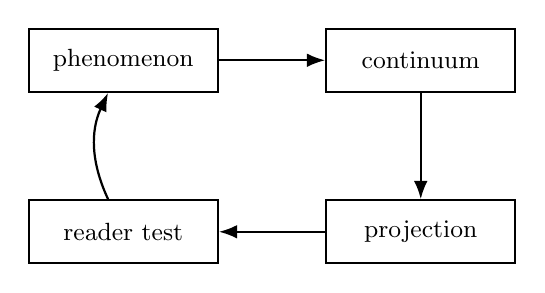
\begin{tikzpicture}[node distance=1.35cm,>=Latex,every node/.style={font=\small}]
\node[draw,thick,align=center,minimum width=2.4cm,minimum height=0.8cm] (a) {phenomenon};
\node[draw,thick,align=center,minimum width=2.4cm,minimum height=0.8cm,right=of a] (b) {continuum};
\node[draw,thick,align=center,minimum width=2.4cm,minimum height=0.8cm,below=of b] (c) {projection};
\node[draw,thick,align=center,minimum width=2.4cm,minimum height=0.8cm,left=of c] (d) {reader test};
\draw[->,thick] (a) -- (b);
\draw[->,thick] (b) -- (c);
\draw[->,thick] (c) -- (d);
\draw[->,thick,bend left=25] (d) to (a);
\end{tikzpicture}
\caption{K-Level Map: phase diagram of domain projection pressure 42-1-37}
\label{fig:figure-the-k-level-map-one}
\end{figure}
The point of the diagram is not decoration; it marks which relation is being proposed and which stronger conclusion is still unavailable.\par
A local clarification is useful here\par
A local clarification is useful here\footnote{In K-Level Map, this note clarifies the reader clarification role of the term and keeps the caveat close to the sentence that needs it.}.\par
The note keeps the caveat near the term without derailing the main sentence.\par
A K-Level is a repeatable level of description. It is not a substance, a hidden force, or a rank in a hierarchy of importance. It marks a place where the relevant objects, boundaries, and transformations can be named without pretending that every other level has disappeared. A car is an object at one K-Level. A traffic wave is an object at another. A commuter dependence between housing and work is an object at another. The bridge is present in all three descriptions, but it is not doing the same explanatory work in each.\par
The stakes appear most sharply when a system meets contradiction. Here contradiction does not mean a mere clash of opinions or a loose inconsistency in language. It means a configuration that demands incompatible continuations under the transformations available to it. A queue must move, but every path by which it could move is blocked. A rule must apply universally, but the case before it exposes an exception the rule cannot absorb. A model requires a boundary to remain fixed while its own operation also requires the boundary to move. When this happens, the system may need a new dimension of description, or it may collapse.\par
Collapse does not always mean physical destruction. The bridge need not fall into the river for the traffic system to collapse. Collapse means that the configuration can no longer continue under the operations that normally sustain it. Cars can still accelerate, brake, and merge, but those actions no longer restore movement. A legal system can still issue decisions, but its categories no longer separate the cases they must govern. A theory can still produce sentences, but its terms no longer apply without contradiction. The K-Level Map matters because it helps locate the level at which continuation has failed.\par
The familiar mistake is to search for the one real explanation. One answer points downward: the real explanation is particles, components, incentives, genes, or signals. Another points upward: the real explanation is the institution, organism, market, ecology, or culture. Both may be true enough to matter. Both become misleading when they erase the work done at intermediate levels. A heartbeat is not false because cardiac cells exist. A cardiac cell is not false because ion channels exist. A diagnosis cannot be replaced by a list of atoms, but it also cannot ignore the body in which it is made.\par
On the bridge, the same event changes its meaning as the description changes. At the driver level, a stalled truck is an obstacle. At the flow level, it is a capacity reduction that may generate a shock wave. At the city level, it exposes dependence on a narrow crossing at a particular hour. These are not decorative ways of saying the same thing. They point to different objects and different possible actions. One tow truck may solve the local obstruction. Signal coordination may soften the flow disruption. A different relation between work schedules, transit, housing, and road capacity may be needed to reduce the citywide vulnerability.\par
The lower description has not become false. The truck still has a failed part, a driver, a location, and a weight. But once the jam has crossed the district, the truck alone is no longer the object that explains the condition. The map prevents a claim from carrying the language of one K-Level into another without paying the cost of translation. It asks where the contradiction lives, what kind of operation could answer it, and whether the system is facing a local repair, a higher-level reconfiguration, or a collapse of its ordinary way of continuing.\par
\section{The K-Level Reading In K-Level Map}
The first word the map needs is object. An object is anything stable enough within a description to be referred to again. It may be a molecule, a road segment, a cell, a policy, a category, a measurement interval, or a theorem statement. The word is broad, but it is not vague. Something becomes an object only relative to a K-Level at which its boundary can be drawn and its behavior can be followed. A single car is an object in one traffic description. A measured flow rate is an object in another. A commuting pattern across a region is an object in a third. \cite{anderson_more_is_different,stauffer_percolation}\par
An operator is an allowed transformation on objects at a given K-Level. Braking, accelerating, merging, closing a lane, changing a signal cycle, adjusting a toll, applying a rule, or transforming a mathematical expression can all be operators if the level of description makes them legitimate. The same physical event may appear under different operators at different K-Levels. Turning a steering wheel is a bodily action for the driver, a change of vehicle trajectory for the road model, and a perturbation in flow for the traffic network.\par
The local dependency can now be written without changing the claim it supports.\par
\begin{equation}\label{eq:equation-the-k-level-map-two}
\operatorname{proofDependency}_{10} = C_{\mathrm{unres}}=\min_{\pi\in\Pi}\|B(x)-B(\pi x)\|
\end{equation}
The relation names a local dependency, variable dictionary, and proof/evidence role; it is not a claim-status upgrade.\par
The formula is a restraint on the prose. It names the dependency that the surrounding paragraph is allowed to use.\par
The comparison below gives k-level map a set of quantities that can be inspected instead of merely admired.\par
\begin{table}[htbp]
\centering\small
\caption{K-Level Map: observable quantities and counter-pressure 42-2-37}
\label{tab:table-the-k-level-map-one}
\begin{tabular}{@{}llll@{}}
\toprule
Boundary & Measured cue & Scale & Failure sign \\
\midrule
k-level map boundary & 33 units & declared case & fixes what is compared \\
residual pressure & 0.77 & dimensionless & shows unresolved load \\
projection loss & 0.34 & bounded interval & marks lost structure \\
countercase set & 16 cases & review sample & keeps a falsifier visible \\
\bottomrule
\end{tabular}
\end{table}
The table should be read locally: it narrows the comparison without pretending that the wider theory has been settled by a single surface.\par
This distinction is not academic. If the object is a car, the operator may be repair, removal, or steering. If the object is a flow, the operator may be rerouting, smoothing, metering, or capacity allocation. If the object is commuting dependence, the operator may be a change in work hours, transit availability, housing distribution, or pricing. A plan that uses the object from one K-Level and the operator from another can sound intelligent while doing nothing. It tells the truck to become a policy, or the policy to move like a truck.\par
A boundary is the condition by which an object is distinguished from what is not that object. Some boundaries are physical, like the edges of a lane or the steel of the bridge. Some are institutional, like a school district or a court's jurisdiction. Some are temporal, like the morning peak. Some are mathematical, like the domain of a function. Boundaries do not all have the same kind of reality, but every serious claim must say which boundary it is using. A neighborhood boundary used by residents may not match a postal zone, a police precinct, a school district, or a data set.\par
A continuum is a field of possible variation within which objects and operators can be described. Temperature varies on one continuum; traffic density on another; trust, legal authority, attention, and connectivity on others. These continua are not secretly the same physical measure. Their shared role is descriptive: each lets a system vary, cross thresholds, and change the stability of its objects. On the bridge, vehicle density is one continuum. At low density, each driver has room to correct. At high density, a small hesitation can travel backward as a wave.\par
Projection is the disciplined translation from one K-Level to another. It may compress detail, expose a pattern, or reveal a mismatch. A traffic engineer may project thousands of individual vehicles into an average flow rate. A public agency may project many flow measurements into a regional reliability score. Projection is not a license to treat unlike things as identical. Something is preserved, something is simplified, and something is lost. The map requires that the loss be acknowledged instead of hidden inside a clean phrase.\par
The bridge example shows why these terms belong together. At the local K-Level, the objects are vehicles, lanes, drivers, distances, and obstructions. The operators include braking, accelerating, merging, signaling, and towing. The boundaries are lane markings, vehicle bodies, sight lines, and the immediate segment of road. The continuum may be speed, spacing, or reaction time. A stalled truck is a local object that can be acted on directly.\par
At the flow K-Level, the objects are no longer mainly individual drivers. They are rates, waves, bottlenecks, queues, and corridors. The operators include ramp metering, signal timing, variable speed limits, and rerouting. The boundaries are not the bumper of the truck but the edges of a corridor, a sensor network, or a time window. The continuum may be density, throughput, delay, or connectivity. The stalled truck has become an event inside a larger object: a pattern of constrained movement.\par
At the urban K-Level, the objects include commuting demand, work schedules, transit substitution, freight timing, housing distribution, and institutional responsibility. The operators include zoning decisions, employer practices, transit investment, toll policy, and emergency coordination. The boundary may be a metropolitan region rather than the bridge itself. The continuum may be dependence: how much of ordinary life must pass through this crossing at this hour. The same morning has not changed its facts, but it has changed the description required to understand it.\par
\section{Completeness Pressure In K-Level Map}
No one needs a K-Level Map to notice that large things are made of smaller things. The harder lesson is that organized systems often display regularities that cannot be handled well by speaking only in the vocabulary of their smallest parts. Philip W. Anderson gave one of the clearest modern statements of this lesson in his argument that more can be different. The point was not that larger-scale patterns float free from physical constraint. It was that new regularities and principles can become necessary when many parts are organized together. \cite{anderson_more_is_different,stauffer_percolation}\par
That insight is easy to misuse. It can become a slogan for mystery, as if every large pattern were automatically beyond ordinary explanation. The K-Level Map takes the opposite lesson. If more can be different, then the difference must be located. What is the new object? What operations act on it? What boundary lets it be distinguished? What lower detail has been gathered, and what has been lost in the gathering? Anderson's warning makes the question unavoidable, but it does not answer it for any particular case.\par
The local dependency can now be written without changing the claim it supports.\par
\begin{equation}\label{eq:equation-the-k-level-map-one}
\operatorname{comparatorDistance}_{10} = \Delta d=\operatorname{rank}(A_{\mathrm{new}})-\operatorname{rank}(A_{\mathrm{old}})
\end{equation}
The relation names a local dependency, variable dictionary, and proof/evidence role; it is not a claim-status upgrade.\par
The formula is a restraint on the prose. It names the dependency that the surrounding paragraph is allowed to use.\par
The local dependency can now be written without changing the claim it supports.\par
\begin{equation}\label{eq:equation-the-k-level-map-three}
\operatorname{leanBinding}_{10} = P_{\mathrm{collapse}}=\sigma(\alpha R-\beta S-\gamma M)
\end{equation}
The relation names a local dependency, variable dictionary, and proof/evidence role; it is not a claim-status upgrade.\par
The formula is a restraint on the prose. It names the dependency that the surrounding paragraph is allowed to use.\par
A small numerical test keeps the abstraction honest at the scale of a single decision.\par
\paragraph{Numerical example.} For k-level map, take support=0.58, projection loss=0.14, and 5 open obligations. The bounded score is 0.; the example gives the reader a numeric scale without pretending to be empirical proof.\par
The numbers are deliberately small; their value is pedagogical, not evidential, unless the chapter binds them to a dataset elsewhere.\par
Percolation theory offers a vivid comparison because it shows how local connections can produce a global transition. In a simple percolation model, many small sites or bonds may be open or closed. Below a threshold, connection remains local. Above it, a spanning cluster appears, and movement across the whole system becomes possible. Nothing supernatural enters the model at the threshold. Yet the relevant object has changed. One is no longer asking only whether neighboring points connect. One is asking whether a connected structure crosses the space.\par
A traffic network can be felt in similar terms, though the mathematics is not being imported wholesale. Each vehicle interaction is local. A driver leaves too little space, brakes slightly, and the driver behind responds. For a while the disturbance remains small. Under the wrong density, the disturbance propagates. The road has crossed from ordinary flow into a state where the pattern itself becomes the object. A backward-moving traffic wave is not a ghost above the asphalt. It is a real object of the flow K-Level because it can be identified, measured, anticipated, and sometimes changed.\par
Renormalization gives another caution. In the sciences where it is used rigorously, it shows how some descriptions become more powerful when microscopic detail is systematically compressed and scale-relevant structure is retained. The K-Level Map does not claim that every field admits that exact mathematics. Its lesson is more basic and more portable: not every detail matters equally at every scale, and the act of moving between scales is itself a disciplined operation. Some variables wash out. Some boundaries become stable only after many smaller differences have been gathered.\par
The bridge again makes the point concrete. A city agency cannot manage morning mobility by knowing the private emotional state of each driver. That detail may matter in a crash investigation, but it usually washes out at the flow K-Level. Density, capacity, timing, and alternative routes remain. At the same time, the agency cannot ignore local detail altogether. A single disabled truck, a badly placed work crew, or a failed signal can trigger a higher-level condition. The art is not choosing detail or abstraction once and for all. It is knowing which K-Level the question requires.\par
A K-Level is earned when a description becomes operationally distinct. First, the local objects and operators must be named honestly. Second, their interactions must create a stable aggregate object that can be referred to without listing every lower object. Third, the aggregate must have operators that are not merely decorative restatements of lower-level motion. Fourth, the projection relation must be stated: what is preserved, what is compressed, and what is lost. A new vocabulary is not enough. A level must do work.\par
Dependence therefore differs from replacement. A sentence depends on letters, but grammar is not well described as a heap of letters. A market price depends on trades, but a price movement is not the same object as any one trade. A tissue depends on cells, but wound healing is not captured by naming cells in isolation. The lower K-Level constrains the higher one; it does not automatically provide the best operator for every question.\par
The reverse error is just as dangerous. If higher-level descriptions forget their lower constraints, they drift into fiction. A policy that treats commuters as infinitely flexible will fail against bodies, wages, childcare, geography, and time. A biological explanation that speaks only of organism-level function may miss the cellular mechanism that blocks the function. A social explanation that treats categories as self-sufficient may miss material limits that make the category unstable. The K-Level Map is built to keep both errors visible at once.\par
\section{A Rival Partition Test In K-Level Map}
The K-Level Map can be used before equations appear. That does not make it casual. Its first work is grammatical and operational: it tells the reader what kinds of symbols could later be introduced without confusion. If a formula contains an object, an operator, a boundary, a continuum, or a projection, the map tells the reader which K-Level that term belongs to and what movement between levels is being claimed. \cite{anderson_more_is_different,stauffer_percolation}\par
An equation surface is the place where prose objects become symbolic objects. At that surface, a term cannot rely on mood or authority. If a symbol names a boundary, the boundary must be identifiable. If it names an operator, the transformation must be describable. If it names a projection, the source and target K-Levels must be known. A term is not placed at a higher K-Level because it sounds more abstract. It belongs there only if the objects and operators of that level require it.\par
The case that follows turns the proposal into a sequence of criticizable moves.\par
\paragraph{Worked case.} In the worked case for k-level map, the claim is reduced to a boundary, an observable, a dependency, a numerical cue, and a falsifier. The case is useful only because each move can be criticized separately.\par
The case helps because each step can fail separately, which is exactly what a useful example should permit.\par
Imagine a clean formula that says local vehicle density produces congestion. It may be useful, but it hides several choices. Is congestion a property of one road segment, a bridge corridor, a district, or an entire city? Is density measured at a moment, averaged over an interval, or inferred from sensors with missing data? Is the operator a change in driver behavior, road capacity, signal timing, or travel demand? Without the map, the equation may look precise while its terms point in different directions.\par
The same problem appears wherever a system crosses scale. In ecology, movement between neighboring habitat patches may matter locally, while the persistence of a population across a landscape belongs to a broader K-Level. In medicine, a molecular pathway, an organ function, a diagnosis, and a patient's treatment plan may all be relevant, but they are not the same object. In law, the same sentence may be a text-level object, a courtroom-level operator, and a society-level boundary condition. The K-Level Map does not collapse these fields into one science. It gives them a shared discipline for declaring where the claim is made.\par
This discipline is especially important when contradiction is present. Suppose the bridge authority says the crossing must carry more vehicles at the peak hour, must lose no lane space, must require no schedule change, must add no transit alternative, and must remain safe. At the local K-Level, the operators are exhausted: cars can only occupy so much space at safe distances. At the flow K-Level, signal timing and speed smoothing may help but may not be enough. At the urban K-Level, the demand itself becomes the object. The contradiction has not been solved by renaming it. It has been located.\par
A formal expression that ignores this location will mislead. It may assign a variable for capacity and a variable for demand, then pretend the gap between them is a mere quantity to be balanced. But the available operations differ by K-Level. Adding capacity, smoothing flow, shifting demand, and redesigning dependence are not interchangeable terms. They belong to different descriptive surfaces. A theory that cannot distinguish them will confuse a bottleneck with a way of life.\par
No required formula is introduced here because the reader first needs the level grammar. Premature notation can give the appearance of precision while postponing the harder question: what is the object, at what K-Level, under which operator, across which boundary, along which continuum, and by what projection? Once those questions are answered, notation can sharpen the claim. Before they are answered, notation only hides the blur.\par
This is also why the map resists grand analogies. It may be tempting to say that a traffic jam, an institutional crisis, and a failed proof are all the same because each involves blockage. The comparison may be useful only after the objects and operators have been declared. In traffic, blockage may concern vehicle flow through space. In an institution, it may concern authority through rules. In mathematics, it may concern inference through assumptions. The map permits comparison by making difference explicit. It does not purchase unity by erasing it.\par
\section{What The Level Adds In K-Level Map}
A K-Level claim carries a burden. It must show that the proposed level is doing work. Naming a new level is not enough. A description earns its place when it identifies objects that persist under relevant variation, operators that act on those objects, and boundaries that distinguish the objects from their surroundings. If these are missing, the language may still be suggestive, but it has not become a disciplined part of the map. \cite{anderson_more_is_different,stauffer_percolation}\par
Hierarchy language can flatter weak arguments. Words such as deep, emergent, structural, systemic, and foundational often make a claim sound larger than its evidence. The map treats none of them as proof. It asks what changes when the K-Level is admitted. Does a new prediction become possible? Does an old contradiction become locatable? Does an intervention become better specified? Does a confused boundary become stable? If not, the proposed level may be unnecessary.\par
Return to the bridge. Saying that the city has a mobility K-Level is useful only if it clarifies something that lane-level description cannot. If the mobility description identifies commute dependence, transit substitution, work-time flexibility, freight timing, and housing distribution as objects in a shared system, it may carry a real claim. If it merely renames traffic as mobility, it adds nothing. The map separates a higher-level object from a fashionable noun.\par
Emergence belongs under the same burden. Emergence is the appearance of a stable pattern or object at one K-Level that is not adequately handled by listing lower-level parts alone. The definition is intentionally modest. It does not say that the higher-level object violates lower-level law. It does not say that the lower K-Level is irrelevant. It says that a new descriptive object has appeared and must be tested for operational standing. The traffic wave emerges from driver interactions, but it earns attention only because it can be tracked and acted on as a flow-level object.\par
Collapse also has to be kept modest. Collapse is the loss of a configuration's ability to continue under its available operators. A traffic network collapses when ordinary flow operations no longer restore movement. A classification collapses when its boundary no longer separates the cases it must separate. A theoretical description collapses when its terms cannot be applied without contradiction. Collapse is not a dramatic label for difficulty. It is a claim about failed continuation.\par
The central hypothesis can now be stated plainly: when a contradiction remains unresolved, the configuration may require a new dimension of description, or it may collapse. This is not offered as a completed theorem. It is a guide for later formal, evidential, and comparative work. The K-Level Map makes the hypothesis intelligible by specifying where contradiction, new description, and collapse can be located.\par
The hypothesis is easy to abuse. If every unresolved problem can be answered by inventing a new K-Level, the map becomes unfalsifiable. That is why the burden matters. A new level is not admitted because the old description is uncomfortable. It must bring identifiable objects, legitimate operators, usable boundaries, and explicit projection rules. It must also expose itself to refusal. If the proposed level cannot distinguish its objects, cannot say what transformations belong to it, or cannot explain what lower detail it compresses, it fails.\par
Another objection says that the map may be too strict because real fields use mixed vocabularies. That objection is right about the world and wrong about the map. The map does not forbid mixed description. It asks mixed description to declare its crossings. A clinician may move from molecule to organ to patient behavior in a single explanation. A climate scientist may move from local measurements to global circulation. A legal theorist may move from text to institution to social effect. The movement is not the problem. Undeclared movement is the problem.\par
The bridge authority does this kind of crossing whenever it acts well. It receives reports from drivers and sensors, estimates corridor flow, coordinates police and towing, communicates with transit systems, and sometimes revises policy. Good practice is already multi-level. The K-Level Map makes that practice explicit enough to test. It asks whether the local incident, the flow disruption, and the citywide dependence have each been described at the level where meaningful action is possible.\par
\section{Why Levels Are Needed In K-Level Map mapS06}
The K-Level Map fails when it becomes decoration rather than constraint. If every difference in vocabulary is called a level, the map dissolves. If every aggregate is called emergent, the word loses force. If every inconvenience is called contradiction, collapse becomes melodrama. The boundary of failure is therefore part of the map itself. A K-Level claim can be rejected. \cite{anderson_more_is_different,stauffer_percolation}\par
The first failure mode is object failure. A proposed level has no stable object. Suppose a commentator says that the city's mood explains the bridge failure. There may be real relations among weather, public events, stress, and travel behavior. Still, mood is not yet an object in the traffic description unless it can be bounded, observed, and connected to operators. Without that work, it remains a suggestive phrase rather than a K-Level object.\par
The second failure mode is operator failure. A proposed level names an object but cannot say what acts on it. A traffic flow can be slowed, redirected, smoothed, measured, or interrupted. These operators make it usable. By contrast, a vague claim that the system's essence changed may express dissatisfaction with the lower description, but it does not establish a new level. A level that cannot be acted on or transformed is not yet doing explanatory work.\par
The third failure mode is boundary failure. A claim cannot say where the object begins or ends. In percolation, the difference between local connection and a spanning cluster depends on a defined lattice, graph, or space. In a city, the relevant network may be the bridge, a road corridor, a transit map, a commuting region, or a sensor grid. If the boundary shifts whenever the argument is challenged, the level claim cannot be trusted.\par
The fourth failure mode is projection failure. A claim moves between K-Levels without preserving enough structure to justify the movement. Local frustration among drivers may contribute to unsafe behavior, but it does not automatically explain housing policy. A molecular interaction may contribute to disease, but it does not automatically explain a patient's access to care. Projection requires a stated relation between levels. Without it, the argument leaps.\par
The fifth failure mode is status inflation. A useful analogy is treated as proof. A plausible model is treated as measured fact. A formal sketch is treated as a completed theorem. A simulation is treated as the world. The K-Level Map cannot by itself prevent these mistakes, but it gives the reader a way to locate them. It asks what kind of claim is being made at each K-Level and what kind of warrant that claim has actually received.\par
The bridge at rush hour is humble enough to keep the lesson honest. Nothing in the example requires believing that traffic, law, biology, and mathematics are one thing. The example shows only that systems can demand different descriptions as their objects change. A truck can be repaired. A flow can be managed. A citywide dependence can be redesigned. Confusing those actions creates bad theory and bad practice alike.\par
The map is therefore a protection against false unity. It allows comparison across domains, but comparison is not sameness. A biological organism, a road network, a legal institution, and a mathematical construction do not become one kind of thing because they can be placed on a shared map. They become comparable only where their objects, operators, boundaries, continua, projections, emergent patterns, contradictions, and collapses have been declared with enough discipline for disagreement to begin.\par
That is the work the K-Level Map must do before heavier claims can be carried. It does not promise that every contradiction will be resolved by climbing to a higher description. Some contradictions are local errors. Some are artifacts of bad language. Some are real failures of continuation. But when a system can no longer proceed under the operations available to it, the map gives the reader a way to ask the next question without panic or inflation: is the object wrong, is the boundary wrong, is the operator exhausted, or has a new level of description become necessary?\par
\chapter{Cross-Level Dependencies and Projection Rules}
\section{Why Levels Are Needed In Cross-Level Dependencies Projection Rules}
A cross level dependency begins with a simple discipline: not every item in a description is the same kind of item. A stone, a crack, a wet patch, a slope, a drainage basin, and a municipal flood warning may all appear in one account of a hillside after rain, but they do not occupy the same descriptive level. Some name material parts. Some name relations among parts. Some name aggregated behavior. Some name decisions made from an aggregated view. OC calls the kind of descriptive item being used a node class. \cite{stauffer_percolation,grimmett_percolation}\par
A node is any identifiable item in the description of a system. A node class states what kind of item it is. In the hillside example, a pore between grains is a microstructural node. A connected wet channel is a mesoscopic node. The whole slope is a macroscopic node. A hazard zone drawn on a planning map is a projected node, because it is not the hillside itself but a domain-facing representation made from selected features of the hillside.\par
The next diagram slows the argument down just enough to show how cross-level dependencies projection rules is being organized.\par
\begin{figure}[htbp]
\centering
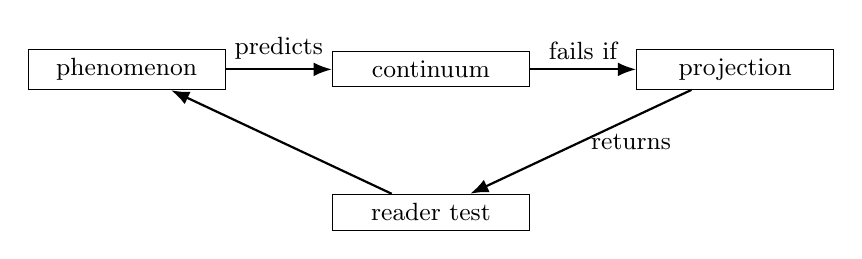
\begin{tikzpicture}[node distance=1.35cm,>=Latex,every node/.style={font=\small}]
\node[draw,align=center,minimum width=2.5cm] (c) {phenomenon};
\node[draw,align=center,minimum width=2.5cm,right=of c] (t) {continuum};
\node[draw,align=center,minimum width=2.5cm,right=of t] (f) {projection};
\node[draw,align=center,minimum width=2.5cm,below=of t] (r) {reader test};
\draw[->,thick] (c) -- node[above]{predicts} (t);
\draw[->,thick] (t) -- node[above]{fails if} (f);
\draw[->,thick] (f) -- node[right]{returns} (r);
\draw[->,thick] (r) -- (c);
\end{tikzpicture}
\caption{Cross-Level Dependencies Projection Rules: falsifier of conceptual dependency pressure 43-1-38}
\label{fig:figure-cross-level-dependencies-and-projection-rules-one}
\end{figure}
The point of the diagram is not decoration; it marks which relation is being proposed and which stronger conclusion is still unavailable.\par
A local clarification is useful here\par
A local clarification is useful here\footnote{In Cross-Level Dependencies Projection Rules, this note clarifies the reader clarification role of the term and keeps the caveat close to the sentence that needs it.}.\par
The note keeps the caveat near the term without derailing the main sentence.\par
The distinction matters because later claims can fail by mixing node classes. A statement about water passing through pores is not automatically a statement about evacuation planning. A statement about a warning map is not automatically a statement about soil physics. The two may be related, and the relation may be important, but the relation has to be named rather than smuggled into the vocabulary.\par
Percolation theory gives a useful neighboring intuition. In the standard picture, sites or bonds may be open or closed, and large-scale connectivity can appear when enough local connections are present. Stauffer and Aharony treat this as a way to study how local occupancy gives rise to extended clusters, while Grimmett gives the mathematical theory a careful probabilistic form. OC does not identify its whole hierarchy with percolation theory, but it borrows a lesson: a local item and a large connected structure are not the same descriptive object, even when one depends on the other.\par
A node class is therefore not an honorific label. It is a constraint on what may be inferred. If a pore is named as a pore, the admissible questions concern local geometry, fluid passage, or material state. If a connected wet channel is named, the admissible questions concern connectivity, directionality, and persistence. If a planning zone is named, the admissible questions concern the projection from physical state into an administrative representation. The name of the node class tells the argument what kind of move is being made.\par
The first work done by this vocabulary is negative. It prevents a sentence from leaping across the hierarchy without paying the cost of translation. A model may say that a local saturation threshold increases the probability of a connected flow path. It may not, from that statement alone, say that a city has a reliable evacuation category. Additional nodes and additional relations are needed: sensors, time windows, terrain maps, institutional thresholds, and the rule by which a physical condition is projected into a public classification.\par
Cross Level Dependencies and Projection Rules therefore cannot begin with the projection. A projection is only intelligible after the source nodes have been classified. If the source is a collection of measurements, one question follows. If the source is an inferred continuum, another follows. If the source is a decision boundary imposed by a public agency, still another follows. The same word, risk, may refer to any of these unless the node class fixes the level at which the word is being used.\par
\section{The K-Level Reading In Cross-Level Dependencies Projection Rules}
After the description has learned to distinguish its items, it has to say how they are related. OC calls a relation between nodes an edge. Edge semantics means the stated meaning of that relation. The relation may be material, causal, statistical, computational, classificatory, or institutional. The edge is not merely a line drawn between boxes. It is a claim about why movement from one node to another is legitimate. \cite{stauffer_percolation,grimmett_percolation}\par
Return to the wet hillside. The relation between a pore and a neighboring pore may be a physical adjacency relation. The relation between many adjacent wet pores and a connected wet channel may be an aggregation relation. The relation between a connected wet channel and a slope-instability estimate may be a modeled dependency. The relation between that estimate and a municipal warning map may be a projection into a practical domain. These are different edge meanings. Treating them as one generic arrow would erase the part of the argument where most errors enter.\par
The local dependency can now be written without changing the claim it supports.\par
\begin{equation}\label{eq:equation-cross-level-dependencies-and-projection-rules-two}
\operatorname{caseCoverage}_{10} = \tau_{\mathrm{repair}}=\inf\{t:C(t)<\theta\}
\end{equation}
The relation names a local dependency, variable dictionary, and proof/evidence role; it is not a claim-status upgrade.\par
The formula is a restraint on the prose. It names the dependency that the surrounding paragraph is allowed to use.\par
The comparison below gives cross-level dependencies projection rules a set of quantities that can be inspected instead of merely admired.\par
\begin{table}[htbp]
\centering\small
\caption{Cross-Level Dependencies Projection Rules: observable quantities and counter-pressure 43-2-38}
\label{tab:table-cross-level-dependencies-and-projection-rules-one}
\begin{tabular}{@{}llll@{}}
\toprule
Claim & Support carrier & Residual & Interpretation \\
\midrule
cross-level dependencies projection rules boundary & 36 units & declared case & fixes what is compared \\
residual pressure & 0.84 & dimensionless & shows unresolved load \\
projection loss & 0.45 & bounded interval & marks lost structure \\
countercase set & 17 cases & review sample & keeps a falsifier visible \\
\bottomrule
\end{tabular}
\end{table}
The table should be read locally: it narrows the comparison without pretending that the wider theory has been settled by a single surface.\par
The vocabulary of edges also protects the status of a claim. A material edge is not a statistical edge. A statistical edge is not a legal authority. A legal authority is not a laboratory observation. A scientific monograph can discuss how these edges interact, but it cannot pretend that one kind of relation has silently become another. If a rain gauge reading contributes to a warning category, the edge from measurement to category may pass through calibration, model selection, threshold policy, and institutional action. Each step changes what is being claimed.\par
Kadanoff's work on scaling and Goldenfeld's lectures on phase transitions and renormalization offer a nearby scientific lesson. Large-scale descriptions often discard microscopic detail in order to reveal patterns that are stable at a different scale. That discard is powerful, but it is not free. The relation between microscopic variables and macroscopic variables has to be controlled by a rule of translation. OC treats this need for controlled translation as a general problem across domains, not only as a problem in statistical physics.\par
An edge can preserve information, compress information, transform information, or authorize action. Preservation occurs when the target node keeps the relevant content of the source node. Compression occurs when many source nodes are summarized into fewer target nodes. Transformation occurs when the same source material is redescribed in another vocabulary. Authorization occurs when a descriptive result is allowed to trigger a decision, such as a warning level, inspection requirement, or exclusion condition.\par
The same edge may also have a direction. Local saturation may contribute to slope instability, but the public warning does not physically wet the soil. The warning may alter human behavior, and that behavior may change load, access, or drainage maintenance, but that is a different loop with different nodes. Directionality matters because cross level explanations often become confused when an effect at one level is read backward as a cause at another.\par
Edge semantics is also where absence becomes visible. If a description says that a microscopic contradiction produces a higher-level form, it must say what edge carries the movement. Is the higher-level form an observed aggregation, a mathematical construction, a classification convenience, or a hypothesis about dynamics? OC can use all of these, but it cannot blur them. The edge label is the local honesty of the hierarchy.\par
\section{Completeness Pressure In Cross-Level Dependencies Projection Rules}
A dependency walk is the ordered passage from one node to another through stated edges. It is the route by which a claim travels across levels. The word walk is deliberately modest. It does not imply that the route is unique, complete, or proven. It means that the route can be followed step by step, with each node class and edge meaning visible along the way. \cite{stauffer_percolation,grimmett_percolation}\par
Consider a practical claim: after prolonged rain, a hillside sector belongs in a higher inspection category. A responsible dependency walk might begin with local measurements of moisture, pass to estimates of pore saturation, pass to connected flow channels, pass to slope-scale instability indicators, pass to an inspection threshold, and end at a category on a planning map. Each step has a different status. Measurements may be noisy. Saturation estimates may depend on a model. Connectivity may be inferred rather than directly observed. The inspection threshold may be conventional rather than natural.\par
The local dependency can now be written without changing the claim it supports.\par
\begin{equation}\label{eq:equation-cross-level-dependencies-and-projection-rules-one}
\operatorname{finiteCheck}_{10} = \operatorname{loss}_{\phi}=1-\frac{|E_{\phi}\cap E_{\mathrm{domain}}|}{|E_{\mathrm{domain}}|}
\end{equation}
The relation names a local dependency, variable dictionary, and proof/evidence role; it is not a claim-status upgrade.\par
The formula is a restraint on the prose. It names the dependency that the surrounding paragraph is allowed to use.\par
The local dependency can now be written without changing the claim it supports.\par
\begin{equation}\label{eq:equation-cross-level-dependencies-and-projection-rules-three}
\operatorname{counterexamplePressure}_{10} = I_{\mathrm{axis}}=\frac{\operatorname{Var}(x\mid a)}{\operatorname{Var}(x)}
\end{equation}
The relation names a local dependency, variable dictionary, and proof/evidence role; it is not a claim-status upgrade.\par
The formula is a restraint on the prose. It names the dependency that the surrounding paragraph is allowed to use.\par
A small numerical test keeps the abstraction honest at the scale of a single decision.\par
\paragraph{Numerical example.} For cross-level dependencies projection rules, take support=0.61, projection loss=0., and 6 open obligations. The bounded score is 0.; the example gives the reader a numeric scale without pretending to be empirical proof.\par
The numbers are deliberately small; their value is pedagogical, not evidential, unless the chapter binds them to a dataset elsewhere.\par
The walk makes this mixed status explicit. It does not weaken the claim merely by showing its components. It gives the claim a form in which it can be examined. If the local moisture readings are missing, the first part of the walk is weak. If the model connecting saturation to instability is disputed, the middle of the walk is weak. If the threshold is a policy choice, the final step must be described as a policy projection rather than a physical law.\par
Percolation again supplies a useful analogy without becoming the whole theory. In a lattice model, local open bonds can produce a spanning cluster. The walk from local bond state to global connectivity is mathematically specific inside that model. Outside that model, in a real hillside, the walk must include measurement, geometry, material heterogeneity, boundary conditions, and the purpose of the projection. Grimmett's probability treatment and Stauffer and Aharony's physical exposition show why connectivity is a serious concept, not a metaphor. OC then asks how such concepts are carried into broader descriptions without losing their level discipline.\par
A different domain makes the same discipline clearer. A genomic variant may be a node at the molecular level: a change in a sequence, perhaps altering a protein or a regulatory region. That variant is not yet a treatment choice. A dependency walk from variant to treatment would need several steps. It may pass from sequence change to predicted molecular function, from molecular function to altered cellular behavior, from cellular behavior to tissue phenotype, from phenotype to clinical classification, from classification to evidence about response, and finally from evidence to a treatment recommendation. The word may is doing real work here. Each step can fail, weaken, or change status.\par
The variant may be well measured while its functional effect remains uncertain. Its functional effect may be plausible in vitro while its tissue-level consequence is unknown. The tissue phenotype may be observed while the response to a drug remains population-level rather than patient-specific. A clinical guideline may authorize a treatment category without proving that the molecular mechanism is complete in every case. The final recommendation is therefore a projected clinical node, not a simple restatement of the original variant. It carries molecular evidence, biological interpretation, population evidence, clinical convention, and patient-specific judgment in one compressed object.\par
This walk prevents a familiar error. One cannot say, without further specification, that a gene causes a treatment. Nor can one say that a treatment recommendation proves the original molecular mechanism. The lower-level node may be necessary for the particular clinical classification, but the classification also depends on assay quality, reference databases, phenotype, evidence thresholds, contraindications, and the purpose of care. The dependency walk does not deny the force of genomic evidence. It protects that force by showing where it enters and where other relations take over.\par
The walk also exposes missing alternatives. A hillside may become dangerous because of saturation, root loss, construction disturbance, freeze-thaw cycles, or prior cracking. A patient may receive a treatment recommendation because of a genomic variant, disease stage, prior therapy, organ function, or patient preference. If a dependency walk includes only one pathway, then the conclusion has the shape of that pathway. It cannot claim to have exhausted the system. This is not a flaw in the walk. It is the reason for writing it down. A bounded walk is more useful than an unbounded assertion.\par
For OC, cross level dependency is not the fact that everything is connected to everything else. That claim is too cheap to do work. A dependency exists when a change, constraint, contradiction, or state at one node class bears on a node in another class through an articulated sequence of edges. The sequence may be incomplete, but incompleteness must be visible. Later scientific claims can then say exactly which walk they depend on, which part is established within the book's materials, and which part remains a disciplined hypothesis.\par
\section{A Rival Partition Test In Cross-Level Dependencies Projection Rules}
A hierarchy becomes scientifically dangerous when two levels say incompatible things and the contradiction is hidden by vocabulary. A local account may say that no individual pore is fully blocked, while a higher-level account says that flow through the region has effectively stopped. These statements need not conflict. Flow can fail at the connected level even when no single pore has the property named blockage. But the apparent contradiction has to be resolved by node class and edge semantics rather than by choosing the more convenient sentence. \cite{stauffer_percolation,grimmett_percolation}\par
OC uses a conflict rule for this purpose. A conflict rule states how to handle incompatible claims that appear at different levels. The first move is classification: identify the node class of each claim. The second move is edge inspection: identify whether the claims are connected by preservation, compression, transformation, or projection. The third move is status discipline: decide whether the conflict is real, apparent, unresolved, or created by an invalid projection.\par
The case that follows turns the proposal into a sequence of criticizable moves.\par
\paragraph{Worked case.} In the worked case for cross-level dependencies projection rules, the claim is reduced to a boundary, an observable, a dependency, a numerical cue, and a falsifier. The case is useful only because each move can be criticized separately.\par
The case helps because each step can fail separately, which is exactly what a useful example should permit.\par
A real conflict occurs when two claims address the same node class under the same conditions and cannot both hold. An apparent conflict occurs when the claims belong to different node classes and can coexist once the levels are separated. An unresolved conflict occurs when the dependency walk is too incomplete to decide. An invalid projection occurs when a claim from one level is carried into another without the edge that would authorize the transfer.\par
The hillside example gives all four cases. If two instruments at the same place and time report incompatible moisture values beyond their error range, that is a real conflict at the measurement level. If no single pore is sealed but the larger channel network no longer conducts, that may be an apparent conflict dissolved by connectivity. If a model predicts instability but there is insufficient information about subsurface structure, the conflict between prediction and field uncertainty may remain unresolved. If a planning map labels a zone safe simply because one local measurement is low, that may be an invalid projection from a local node into a public category.\par
The genomic example gives a second view. A sequencing assay may identify a variant, while another assay, using a different method or sample, does not. If both address the same molecular node under comparable conditions, the conflict may be real at the measurement level and require technical resolution. If the variant is present but no tissue phenotype appears, the conflict may be apparent or unresolved, depending on penetrance, context, and the biological model. If a treatment category is assigned solely from a variant whose clinical significance is unknown, the conflict is not between biology and care. It is an invalid projection from a molecular node into a treatment node without the necessary connecting edges.\par
The conflict rule is especially important for emergence. Emergence is the appearance of a property, behavior, or descriptive necessity at one level that is not simply present as the same property at a lower level. The term does not license mystery. It marks a demand for a dependency walk. When a connected cluster appears in percolation, global connectivity is not the same kind of statement as the state of one bond. Kadanoff's scaling picture and Goldenfeld's exposition of collective behavior help show why new effective descriptions can become appropriate at larger scales. OC treats emergence as requiring this kind of level-aware account.\par
The rule also protects against reductionist overreach. A lower-level account may be necessary without being sufficient for the higher-level claim. Soil particle geometry may matter for slope behavior, but a public warning category also involves time, exposure, infrastructure, and decision criteria. A genomic variant may matter for a diagnosis or treatment class, but clinical use also involves uncertainty, evidence quality, disease context, and the purpose of the intervention. Saying this does not deny the lower-level basis. It prevents basis from being mistaken for the whole projected claim.\par
The reverse error is just as common. A higher-level classification may organize action, but it does not rewrite the lower-level facts. Calling an area high risk does not specify which pore channels are open. Calling a patient high risk does not specify every molecular mechanism. Calling a market unstable does not identify every trade-level cause. Higher-level nodes can guide attention and action, but their authority over lower-level detail depends on the edges that connect them.\par
The conflict rule therefore has a modest but central role. It keeps contradiction productive. A contradiction may reveal a missing node, a missing edge, a false aggregation, a failed projection, or a genuine instability in the system being described. OC's larger hypothesis concerns the fate of unresolved contradiction, but that hypothesis can only be stated responsibly after the hierarchy has a way to distinguish levels and inspect conflicts among them.\par
\section{What The Level Adds In Cross-Level Dependencies Projection Rules}
Projection is the act of carrying a selected description from one level or domain into another form for a specific purpose. The result is a projected node. A flood map, a clinical score, a supply-chain dashboard, and a phase diagram are not the raw systems they describe. They are constructed views that preserve some features, suppress others, and make certain questions easier to ask. \cite{stauffer_percolation,grimmett_percolation}\par
The word project has two senses here. First, it means to cast a description into a target space, as a terrain model may be cast into a map. Second, it means to make a description useful for a project, such as inspection, comparison, control, or explanation. A projection rule states how the casting is done and what use the result may bear. Without a projection rule, the target object may look precise while its relation to the source remains unclear.\par
In the hillside case, a projection rule may say that measured rainfall, slope angle, soil type, prior saturation, and mapped drainage are combined into an inspection category. This rule does not make the category identical to the hillside. It makes the category a disciplined representation for a particular activity. The category may be useful even though it is coarser than the physical system. It may also be wrong, stale, or too crude for a new question.\par
In the clinical case, a projection rule may say that a variant belongs to a treatment-relevant class only if measurement quality, variant interpretation, disease context, and evidence threshold are all satisfied. The projected node is then not the variant alone. It is a clinical classification produced from selected molecular and medical facts. That classification may guide action, but it should not be read backward as complete knowledge of mechanism. Nor should the existence of a mechanism be treated as automatic permission for a treatment category. The rule tells the reader what has been selected, what has been transformed, and what the resulting node is allowed to support.\par
Projection rules are necessary because no domain receives a hierarchy whole. A public works office does not receive every pore state. A physicist does not receive every municipal concern when studying a lattice. A physician does not receive every molecular event when reading a risk score. Each domain accepts a reduced object under rules that determine what has been kept. The quality of the projection lies not in pretending that nothing was lost, but in knowing what was lost and whether the loss matters for the target claim.\par
This is where scaling ideas again provide a useful comparison. In statistical physics, one often seeks variables that remain meaningful when microscopic detail is coarse-grained. Goldenfeld emphasizes how collective behavior can be described by variables that are not simple restatements of every lower-level fact. Kadanoff's scaling approach makes clear that the move from fine detail to effective description is a controlled intellectual operation. OC generalizes the caution: whenever a description crosses from one level into another domain, the rule of crossing must be stated.\par
A projection may be faithful for one question and unfaithful for another. A flood map may be adequate for deciding where to place temporary barriers, yet inadequate for reconstructing the precise subsurface path of water. A clinical score may help stratify follow-up, yet fail to explain a mechanism. A market index may summarize movement, yet hide the distribution of stress among firms. The projection is not exposed as false merely because it is partial. It becomes false when its partiality is denied or when it is used for a question its rule does not cover.\par
This vocabulary of projection also blocks a common temptation in cross-domain theory. Similar shapes across domains do not automatically mean identical mechanisms. A branching river network, a branching blood vessel structure, and a branching organizational chart may all invite comparison. The comparison may be fruitful, but the projection rule must say what is being compared: topology, flow constraint, growth process, control relation, or visual analogy. Without that rule, resemblance becomes a substitute for analysis.\par
Projection rules carry the burden of later domain claims. If OC describes a continuum in one domain and then uses it in another, the claim cannot rest on shared words alone. It must state what source nodes are selected, what edges are preserved or transformed, what target nodes are produced, and what questions the target nodes can answer. The result may be narrow, but narrowness is a virtue when it marks the actual reach of the description.\par
A final distinction matters. Projection is not publication, persuasion, or simplification for convenience. It is an operation inside the theory's descriptive machinery. A simple explanation may omit details for ease. A projection rule omits or transforms details according to a stated relation between source and target. The former belongs to pedagogy. The latter belongs to the object being claimed.\par
\section{Why Levels Are Needed In Cross-Level Dependencies Projection Rules dependen}
The inspection test asks whether a cross level claim can be followed without guessing the missing machinery. It is not a demand that every claim be final or complete. It is a demand that the claim reveal its node classes, edge meanings, dependency walk, conflict handling, and projection rule. A claim that cannot pass this test may still be suggestive, but it is not yet ready to carry later scientific weight. \cite{stauffer_percolation,grimmett_percolation}\par
Take the sentence: local saturation causes public risk. It sounds plausible, but it fails inspection. Local saturation names a lower-level physical state. Public risk names a projected administrative or practical category. The edge between them is missing. The walk is missing. The projection rule is missing. The conflict rule is missing. The sentence may become usable only after it is rebuilt: measured rainfall and soil moisture estimate pore saturation; saturation contributes to connected subsurface flow under specified terrain conditions; connected flow contributes to a slope-instability indicator; the indicator enters a public inspection category through a stated threshold rule. The rebuilt version is longer because it is carrying the real structure of the claim.\par
The same test applies to a sentence such as: this variant determines treatment. The statement compresses too much. A variant is a molecular node. Treatment is a clinical and institutional action node. Between them lie assay reliability, variant interpretation, biological function, disease context, evidence of response, contraindications, patient state, and the rule by which a clinical category becomes a recommendation. The sentence may be defensible after the walk is supplied, but it is not defensible merely because the endpoint sounds medically precise.\par
The inspection test also catches overconfident emergence language. A sentence such as a new level emerges from contradiction is not yet an operational claim. It must say which contradiction, at which node class, under which constraints, by which dependency walk, and with what higher-level node produced. It must also say whether the higher-level node is observed, modeled, inferred, or proposed. Only then can the statement be evaluated rather than admired.\par
The test has a positive use as well. It shows where a claim is strong enough for its purpose. A percolation model may give a clean account of how local open bonds lead to large-scale connectivity inside its formal setting. The inspection test would identify the node classes as bonds, sites, clusters, and spanning structures; the edges as occupancy and connectivity relations; and the conflict rule as internal to the model's definitions and probability statements. If the same language is carried into geology, epidemiology, or infrastructure, new projection rules are required. The original model remains valuable, but its travel is not automatic.\par
This discipline keeps OC from claiming more than it has earned. The book may introduce a vocabulary for continua, boundaries, operators, hierarchy, contradiction, emergence, collapse, and projection. It may use mathematical analogies and neighboring scientific traditions. It may state proposed operational relations. But it must not treat a vocabulary as evidence, an analogy as a result, a projected category as a raw observation, or a formal-looking sentence as a demonstrated theorem.\par
A first-time reader needs this apparatus before later scientific claims can be trusted because the later claims will move. They will move from local to global, from material to formal, from model to domain, from contradiction to reclassification, and from description to projected use. Without node classes, the levels blur. Without edge semantics, arrows become decoration. Without dependency walks, conclusions appear from nowhere. Without conflict rules, contradictions are either ignored or overdramatized. Without projection rules, domain claims inherit authority they have not been given.\par
The handoff is now precise. The hierarchy is not a ladder of prestige, with lower levels crude and higher levels refined. It is a working arrangement among descriptive levels. Some levels expose material detail. Some expose collective structure. Some expose decision-relevant projections. Cross level dependencies say how one level bears on another. Projection rules say how a description is carried into a target form. The next scientific use of OC can now be asked a concrete question: show the nodes, show the edges, show the walk, show the conflict handling, and show the projection before asking the claim to bear weight.\par
That demand is deliberately sober. It does not forbid analogy, generalization, or movement between domains. It makes such movement answerable. Similar shapes may open inquiry; they do not close it. A structure may resemble another structure in topology, dynamics, constraint, or visible form, and each resemblance may matter in a different way. Cross level work becomes reliable only when the resemblance is converted into a stated projection and the projection is tied back to its dependency walk. Then the theory can travel without pretending that travel is identity.\par
\part{mathematics}
\chapter{Formal Objects of the Theory}
\section{The First Formal Move In Formal Objects of Theory}
Imagine a wet hillside after several days of rain. At first the scene looks simple: soil, water, roots, slope, gravity. A walker sees puddles collecting in shallow places and thin streams finding the lowest channels. A civil engineer sees load, drainage, shear, and risk. A biologist sees root networks and microbial change in saturated ground. A local resident sees whether the retaining wall behind the house will hold. Each description is legitimate, but none is the whole object. The hillside is not only a physical body, not only a hydrological route, not only a biological habitat, and not only a hazard. It becomes a system when a question selects a bounded configuration whose internal relations matter. \cite{grimmett_percolation,goldenfeld_lectures}\par
That last sentence already changes the language. In ordinary speech, a system may mean almost any organized thing. In OC Core 1.4, the name is promoted to a formal object. A formal object is not a new substance in the world. It is a declared object of description: something the theory can name, constrain, compare, and reject. OC itself, in this chapter, means a proposed language for describing ordered contradictions across systems without pretending that hillsides, cells, hospitals, markets, and courts are made of the same material. Its ambition is comparative, but the comparison begins with discipline. The same word may appear first in common speech and then return with a narrower role. A reader can hear the narrowing when it happens.\par
The next diagram slows the argument down just enough to show how formal objects of theory is being organized.\par
\begin{figure}[htbp]
\centering
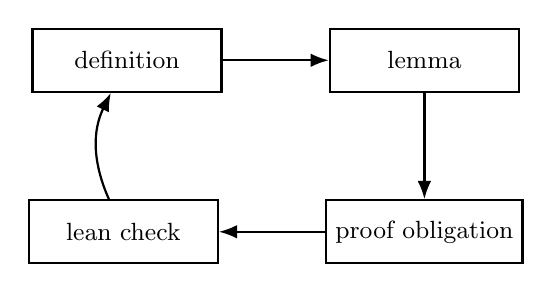
\begin{tikzpicture}[node distance=1.35cm,>=Latex,every node/.style={font=\small}]
\node[draw,thick,align=center,minimum width=2.4cm,minimum height=0.8cm] (a) {definition};
\node[draw,thick,align=center,minimum width=2.4cm,minimum height=0.8cm,right=of a] (b) {lemma};
\node[draw,thick,align=center,minimum width=2.4cm,minimum height=0.8cm,below=of b] (c) {proof obligation};
\node[draw,thick,align=center,minimum width=2.4cm,minimum height=0.8cm,left=of c] (d) {lean check};
\draw[->,thick] (a) -- (b);
\draw[->,thick] (b) -- (c);
\draw[->,thick] (c) -- (d);
\draw[->,thick,bend left=25] (d) to (a);
\end{tikzpicture}
\caption{Formal Objects of Theory: state transition of proof dependency pressure 44-1-39}
\label{fig:figure-formal-objects-of-the-theory-one}
\end{figure}
The point of the diagram is not decoration; it marks which relation is being proposed and which stronger conclusion is still unavailable.\par
A local clarification is useful here\par
A local clarification is useful here\footnote{In Formal Objects of Theory, this note clarifies the reader clarification role of the term and keeps the caveat close to the sentence that needs it.}.\par
The note keeps the caveat near the term without derailing the main sentence.\par
Now suppose a crack appears near the top of the slope. Water enters it, roots bind part of the soil, clay swells below it, and a small section begins to move. One vocabulary says that water has reduced friction. Another says that the slope has crossed a stability threshold. Another says that a connected path through saturated pores has appeared. The last phrasing stands near percolation theory, which studies how local connections can produce large-scale connectivity. The hillside has not become a theorem in percolation theory. The analogy is smaller and more useful: a relation that begins locally may change the status of a larger configuration once enough connections matter.\par
This is why the theory cannot begin with a list of shared materials. A hillside has water pressure, grains, roots, cracks, and drainage channels. A legal institution has offices, texts, incentives, procedures, precedents, and enforcement powers. A cell has membranes, enzymes, signals, energy gradients, and molecular traffic. A financial market has prices, contracts, liquidity, expectations, and rules of settlement. A hospital has bodies, beds, staff, protocols, waiting rooms, machines, budgets, and triage decisions. If OC tried to compare these domains by pretending they contained the same things, it would fail at once. The common language has to be more modest. It must say what counts as the system under discussion, how its boundary is drawn, what can vary, what acts on what, and when a description has changed its level or object.\par
Ordinary language hides these changes of level with remarkable efficiency. A person may say, "the slope failed." The sentence is useful, but it compresses many events: local saturation, deformation, loss of cohesion, propagation of a crack, acceleration of a mass, and the appearance of a new surface. It also compresses a change in objecthood. Before the failure, the hillside was treated as one object with internal variation. After the failure, the moving mass and the remaining slope must be described separately. A language for ordered variation has to make that transition visible without claiming more precision than the case supplies.\par
The same compression appears in less physical cases. A hospital may be said to be "overwhelmed," but that phrase can mean that beds are full, nurses are unavailable, intake is delayed, oxygen supply is constrained, discharge cannot proceed, or decision authority has become unclear. A court may be said to have "lost legitimacy," but the phrase may refer to compliance, public trust, procedural fairness, enforcement capacity, or the ability of judgments to settle disputes. A cell may be said to be "stressed," but the relevant description may concern energy supply, membrane transport, protein folding, immune signaling, or damage repair. In each case the common phrase points toward a real condition while leaving the formal object uncertain.\par
Contradiction enters here, but not yet as a logical puzzle on a page. In OC, contradiction becomes technical only when competing requirements, tendencies, constraints, or descriptions cannot be jointly maintained by the current configuration. The hillside must remain continuous enough to function as the slope being described, while part of it begins to separate along a developing rupture. Soil must transmit load, while saturation weakens the transmission. A hospital must treat urgent cases quickly, while the same emergency conditions consume the staff and space needed for treatment. A constitution may require equal treatment, while administrative practice distributes access unequally. These are not contradictions merely because a writer can phrase them as oppositions. They become contradictions in the theory only when the selected system cannot satisfy the demands together under the description being used.\par
The hillside will remain the opening example because it lets the formal objects be seen without much institutional background. It should not become the whole argument. The theory is interested in the way descriptions travel across domains and then stop. A slope, a hospital, a cell, and a court can all be described as systems with boundaries, axes of variation, operators, projections, contradictions, and possible reconfigurations. That does not make them versions of one master object. It gives the reader a way to ask what has been preserved in the comparison and what has been lost.\par
Formal objects are needed because the alternative is unstable prose. Without them, the theory would say that things have boundaries, that tensions emerge, that systems collapse, or that new dimensions appear, but it would not say what kind of object is being described when those words are used. The chapter therefore begins with a minimum vocabulary: system, boundary, continuum, axis, operator, projection, contradiction, emergence, and collapse. These terms do not prove OC Core 1.4. They specify the grammar in which later claims can become clear enough to test, narrow, formalize, or reject.\par
\section{Axes Before Continua In Formal Objects of Theory}
A formal object in OC is a named kind of entity used to state a claim about a system without depending on the materials of one domain. It is formal because its role is defined by relations, operations, and limits of description, not by a particular substance. It is an object because it can be referred to, compared, constrained, and rejected. The word does not imply that every such object has already been implemented in a proof assistant, measured in a dataset, or confirmed by experiment. It means that the theory declines to leave its basic nouns as evocative metaphors. \cite{grimmett_percolation,goldenfeld_lectures}\par
System is the first of these objects because every later claim needs something accountable to be about. In OC, a system is a bounded configuration whose internal relations matter to the question under discussion. A hillside can be a system for geotechnical analysis. A hospital can be a system for studying triage. A cell can be a system for studying membrane regulation. The definition is operational. A system is not whatever happens to exist. It is the configuration selected under a description because its parts, relations, and limits affect the claim being made.\par
The local dependency can now be written without changing the claim it supports.\par
\begin{equation}\label{eq:equation-formal-objects-of-the-theory-two}
\operatorname{transitionThreshold}_{10} = \rho_{\mathrm{replay}}=\frac{N_{\mathrm{matched}}}{N_{\mathrm{declared}}}
\end{equation}
The relation names a local dependency, variable dictionary, and proof/evidence role; it is not a claim-status upgrade.\par
The formula is a restraint on the prose. It names the dependency that the surrounding paragraph is allowed to use.\par
The comparison below gives formal objects of theory a set of quantities that can be inspected instead of merely admired.\par
\begin{table}[htbp]
\centering\small
\caption{Formal Objects of Theory: observable quantities and counter-pressure 44-2-39}
\label{tab:table-formal-objects-of-the-theory-one}
\begin{tabular}{@{}llll@{}}
\toprule
Model & Retained insight & Rejected assumption & OC extension \\
\midrule
formal objects of theory boundary & 39 units & declared case & fixes what is compared \\
residual pressure & 0.00 & dimensionless & shows unresolved load \\
projection loss & 0.56 & bounded interval & marks lost structure \\
countercase set & 18 cases & review sample & keeps a falsifier visible \\
\bottomrule
\end{tabular}
\end{table}
The table should be read locally: it narrows the comparison without pretending that the wider theory has been settled by a single surface.\par
Boundary follows immediately, because a system without a boundary is only a gesture toward complexity. A boundary is the rule, material condition, interface, or distinction that determines what belongs to the system for the current analysis and what counts as crossing into or out of it. The surface of the hillside may be a spatial boundary. The water table may be a functional boundary. A legal jurisdiction is an institutional boundary. A cell membrane is a biochemical boundary. A boundary can be sharp, porous, mobile, contested, or scale-dependent. The important point is not that all boundaries resemble walls. The important point is that a claim changes when the boundary changes.\par
Continuum is more delicate because the word carries strong associations in mathematics and physics. OC uses it in a broader and weaker sense unless a later argument explicitly narrows it. A continuum is an ordered range of possible states or degrees along which a system can vary under a chosen description. Moisture content in soil may be treated as a continuum. Displacement may be treated as another. Institutional legitimacy may be represented less directly, through observable indicators or structured judgments, but it can still be discussed as a continuum if the analysis states how variation is being ordered. The term does not assert smoothness, differentiability, continuous measurement, or a mathematical field in the technical sense. It marks an ordered space of variation that must be named before an argument can move through it.\par
An axis is a selected direction of variation within such an ordered range. In the hillside case, saturation, shear strength, connectivity of water paths, and displacement may be treated as axes. In a hospital, queue length, acuity, staff availability, bed capacity, and decision latency may function as axes. In a legal institution, compliance, coercion, legitimacy, procedural access, and administrative capacity may be axes. An axis is not a decorative label. It tells the reader what kind of difference is being tracked. If an argument says that a configuration moves from stability toward collapse, the relevant axes have to make that movement intelligible.\par
Operator is another term that must be handled without borrowing false prestige from mathematics. In OC, an operator is an action, process, rule, or transformation that changes the state of a system along one or more axes. Rainfall can operate on saturation. Drainage can operate on pore pressure. Root growth can operate on cohesion. A triage protocol can operate on patient flow. A court ruling can operate on institutional authority. A metabolic signal can operate on cellular response. The term is broad, but not atmospheric. To count as an operator in a claim, it needs an identified domain of action, an affected object or relation, and a possible result. OC does not require a fully specified algebra in every case, but it does require change to be located rather than narrated as force from nowhere.\par
Projection names the movement from one description of a system to another. The hillside can be projected into a geotechnical description, a hydrological description, an ecological description, or a risk-management description. Each projection preserves some relations and ignores or compresses others. Projection is necessary because no single description contains every relevant property at every scale. It is also dangerous because it can import certainty from one domain into another where that certainty has not been earned. OC treats projection as a formal object so that later arguments can state what has been preserved, what has been lost, and where comparison stops.\par
Contradiction, in this vocabulary, is an unresolved incompatibility among requirements, tendencies, constraints, or descriptions that the current system cannot satisfy together. This is narrower than everyday disagreement and broader than formal logical contradiction. It does not mean that two sentences have simply been written in opposition. It means that the configuration itself, under the selected description, cannot continue to maintain the relevant demands without change. In the hillside, the soil mass may be described as continuous while a developing rupture begins to divide it. In a hospital, the intake procedure may need to preserve equal access while emergency scarcity forces selection by urgency, delay, and available capacity. In an institution, a rule may require impartial entry while the actual process blocks a class of participants. The contradiction belongs to a stated description, not to a mood of tension.\par
Emergence is the appearance of a new level, axis, relation, or object that was not adequately present in the prior description. It is not a license to call every surprising outcome emergent. A connected drainage path appearing from many local pore connections is a modest example when it reorganizes the behavior of the slope. A new legal category may emerge when existing categories cannot handle a conflict that practice repeatedly presents. A collective variable may emerge in a model when the relevant behavior at a scale cannot be handled by tracking every local detail. Emergence in OC has to be tied to a stated system, a prior description, and a reason the new object or axis is needed.\par
Collapse is the failure of a configuration to maintain the relations required by its current description. It may be physical, institutional, conceptual, or operational, depending on the system. A landslide is a physical collapse of slope continuity. A failed procedure may be an institutional collapse of decision capacity. A model that cannot distinguish two cases it needs to distinguish may undergo conceptual collapse. Collapse does not mean total destruction, catastrophe, or moral failure. It means that the object can no longer be treated as the same functioning configuration under the terms that defined it.\par
These definitions prepare the central schema rather than establish it as a general law. OC proposes that, when a contradiction remains unresolved within a configuration that cannot jointly satisfy its demands, the analysis should look for one of two constrained outcomes: a re-description that introduces a new object, axis, level, or boundary; or a collapse of the prior configuration under the stated terms. This is a schema for inquiry, not a verdict delivered in advance. Many tensions are absorbed by repair, damping, adjustment, substitution, or changed conditions. The proposed schema begins to matter only when those ordinary resolutions no longer preserve the description.\par
\section{Operators And Their Burden In Formal Objects of Theory}
The hillside can now be redescribed in the vocabulary just introduced. The system is not the entire landscape, the weather, or the regional geology in all their detail. For the present claim, the system is the saturated slope section above the retaining wall, selected because its internal relations determine whether the slope remains continuous or separates into a moving mass and a residual slope. The boundary is partly spatial: the relevant section of soil, root network, drainage paths, and slope face. It is also functional: water enters from rainfall and subsurface flow, load passes through soil structure, and movement across a rupture surface would mark a decisive change in the object. \cite{grimmett_percolation,goldenfeld_lectures}\par
The continua are ordered ranges of variation within that system. Saturation can increase or decrease. Pore pressure can rise or fall. Shear strength can be maintained or reduced. Connectivity among water-filled pores can remain local or become slope-spanning. Displacement can remain negligible or become measurable movement. Each continuum is not equally precise in every observation. Saturation may be measured directly in some settings and inferred in others. Connectivity may be modeled rather than seen. Displacement may be detected by instruments or by cracks and surface changes. The formal point is that the claim has named the ranges along which the system varies.\par
The local dependency can now be written without changing the claim it supports.\par
\begin{equation}\label{eq:equation-formal-objects-of-the-theory-one}
\operatorname{operatorBurden}_{10} = G=(V_{\mathrm{claim}}\cup V_{\mathrm{evidence}},E_{\mathrm{support}}\cup E_{\mathrm{challenge}})
\end{equation}
The relation names a local dependency, variable dictionary, and proof/evidence role; it is not a claim-status upgrade.\par
The formula is a restraint on the prose. It names the dependency that the surrounding paragraph is allowed to use.\par
The local dependency can now be written without changing the claim it supports.\par
\begin{equation}\label{eq:equation-formal-objects-of-the-theory-three}
\operatorname{graphWalk}_{10} = \epsilon_{\mathrm{domain}}=\max_i |y_i-\hat y_i|
\end{equation}
The relation names a local dependency, variable dictionary, and proof/evidence role; it is not a claim-status upgrade.\par
The formula is a restraint on the prose. It names the dependency that the surrounding paragraph is allowed to use.\par
A small numerical test keeps the abstraction honest at the scale of a single decision.\par
\paragraph{Numerical example.} For formal objects of theory, take support=0.44, projection loss=0.12, and 1 open obligations. The bounded score is 0.160; the example gives the reader a numeric scale without pretending to be empirical proof.\par
The numbers are deliberately small; their value is pedagogical, not evidential, unless the chapter binds them to a dataset elsewhere.\par
The axes are the selected directions that matter to the analysis: increasing saturation, decreasing effective strength, increasing hydraulic connectivity, and increasing displacement. The operators are the processes that move the system along those axes. Rainfall increases water input. Drainage removes or redistributes water. Soil texture shapes retention. Roots contribute cohesion in some zones while channels along root paths may also alter flow. Gravity acts continuously through the slope. A new crack changes the boundary conditions by giving water a path and by reorganizing stress around the opening. None of these operators alone is the landslide. Each acts on a specified relation or range of variation.\par
Projection then allows several descriptions of the same system. In a hydrological projection, the main concern is how water enters, moves, accumulates, and drains. In a mechanical projection, the concern is load, strength, deformation, and rupture. In an ecological projection, root structure and soil life become more prominent. In a risk projection, the relevant object includes the retaining wall, house, road, or people below the slope. Each projection preserves something and loses something. The risk projection may preserve the consequence of failure while compressing pore-scale detail. The hydrological projection may preserve flow relations while making the wall nearly invisible. The formal discipline lies in saying which projection is being used when the claim is made.\par
The contradiction can now be stated without drama. Under the mechanical description, the slope section is being treated as a continuous load-bearing configuration. At the same time, saturation, pore pressure, and rupture development may require part of it to move as a separate mass. The configuration cannot indefinitely maintain both the continuity required by the original slope description and the separation implied by developing displacement. If drainage reduces pressure or roots and soil structure maintain cohesion, the contradiction may be resolved without emergence or collapse. If not, the prior description becomes insufficient.\par
Two outcomes then become intelligible, though neither is guaranteed by vocabulary alone. Emergence occurs if a new object or level of description becomes necessary: a moving soil mass, a rupture surface, a drainage channel that reorganizes the slope, or a risk zone that did not previously exist as the relevant object of analysis. Collapse occurs if the slope section can no longer maintain the relations that allowed it to be treated as a continuous stable configuration. In ordinary speech one may still say, "the slope failed." In formal prose, the statement becomes more inspectable: this bounded slope section, under these axes and operators, could not maintain continuity under the selected description, and the analysis now requires either a new object or the recognition that the previous object has lost its defining relations.\par
The same form can be carried, carefully, to a hospital without claiming that hospitals are hillsides. The system might be the emergency department during a surge. The boundary may include intake, triage, treatment rooms, staff assignment, bed transfer, and discharge links to the rest of the hospital. Continua may include patient acuity, waiting time, bed capacity, staff availability, and decision latency. Operators include ambulance arrivals, triage rules, staffing changes, discharge delays, supply constraints, and administrative overrides. A contradiction appears if the department must preserve both timely access for urgent cases and procedural fairness for all entrants while capacity prevents both from being maintained under the existing process. Emergence might take the form of a new triage category, a temporary command structure, or a new boundary between emergency care and overflow care. Collapse would mean that the existing decision procedure no longer performs the relations that made it the procedure it claimed to be.\par
In a court, the same grammar is again altered by the domain. The system may be a claims process rather than a building or a state. The boundary is drawn by jurisdiction, standing, filing rules, hearing procedures, and enforcement links. Continua include access, delay, compliance, interpretive stability, and legitimacy. Operators include statutes, rulings, administrative rules, filing costs, precedent, political pressure, and enforcement practice. A contradiction arises when equal access is required by the governing description while the operational procedure systematically prevents a class of claims from being heard. Emergence may appear as a new category, remedy, procedural right, or institutional forum. Collapse appears when the process no longer maintains the relations that justified calling it an impartial procedure. The comparison is formal, not material. Water does not become precedent; soil does not become law. The role of system, boundary, axis, operator, projection, contradiction, emergence, and collapse is what travels.\par
\section{A Claim Made Inspectable In Formal Objects of Theory}
The vocabulary sits near several established scientific, mathematical, and philosophical ideas. The nearness is useful, but it can mislead. A physicist may hear continuum and expect differential equations. A mathematician may hear operator and expect a precise mapping between spaces. A philosopher may hear ontology and expect a theory of what ultimately exists. A systems theorist may hear emergence and expect a long debate about reduction, organization, and levels. OC does not inherit those meanings wholesale. It borrows ordinary words, places them under declared constraints, and leaves room for stricter formulations where particular domains allow them. \cite{grimmett_percolation,goldenfeld_lectures}\par
The continuum of physics and mathematics is the most obvious neighbor. In many physical theories, a continuum is a domain in which quantities vary smoothly over space, time, or another parameter. Fluids, fields, and elastic bodies are often modeled this way. OC's continuum is deliberately less specific. It may include smooth variation, but it may also include ordered but coarse variation, ranked states, or a constructed descriptive scale. The broader usage is defensible only if its limits remain visible. When a later chapter speaks of a continuum in an empirical or institutional domain, the word does not automatically claim smoothness, differentiability, or direct measurement. It claims an ordered range whose construction has to be stated.\par
The case that follows turns the proposal into a sequence of criticizable moves.\par
\paragraph{Worked case.} In the worked case for formal objects of theory, the claim is reduced to a boundary, an observable, a dependency, a numerical cue, and a falsifier. The case is useful only because each move can be criticized separately.\par
The case helps because each step can fail separately, which is exactly what a useful example should permit.\par
Scaling theory stands nearby because many systems change their descriptive character when one moves between local and global views. Kadanoff's work on scaling and Wilson's development of renormalization altered how physicists think about cases where large-scale behavior cannot be read naively from microscopic detail. Goldenfeld's lectures show how patterns can become stable across changes of scale and how different microscopic systems may share large-scale descriptions. OC is not renormalization group theory. It does not gain equations by speaking about levels. The lesson it takes is narrower: a responsible theory of systems has to say which description is active at which scale, and it has to avoid confusing local detail with global form.\par
Percolation is nearby for a related reason. Percolation theory studies how connectivity arises when local links or sites are present with some probability. It is useful for thinking about thresholds: below some conditions, connections remain local; above them, a spanning structure may appear. The wet hillside can be described with this analogy when water-filled paths begin to connect across a slope. The analogy does not establish that all OC systems are percolation systems. It shows one disciplined pattern: local relations may acquire system-level significance once connectivity changes. The proof burden remains in the target domain.\par
General systems theory is a broader neighbor. Many traditions have tried to describe systems across biology, society, technology, and cognition. OC shares the wish to compare domains without reducing them to one material substrate. Its difference lies in the emphasis on explicit formal objects and projection discipline. A broad systems vocabulary can become too permissive if every organized thing is called a system and every change is called emergence. OC narrows the discussion by asking what boundary, continuum, axis, and operator are active in the claim. The question is not whether a thing sounds systemic. The question is whether the description can be made accountable.\par
Philosophical ontology is nearby because this chapter speaks of objects. Yet the object here is not a declaration of ultimate being. OC is closer to a working metaontology of description: it asks what kinds of objects a theory needs in order to compare systems without erasing domain differences. It does not begin by announcing the final furniture of reality. It begins by defining the objects that have to be present when a claim about a system is made. That difference keeps the theory from becoming metaphysics too quickly. The formal object is a disciplined instrument of description before it is anything else.\par
Formal proof is another neighbor and another temptation. A formal proof system can define terms and derive consequences under exact rules. OC's formal objects are compatible with later formalization where a precise fragment is available. Some terms may eventually receive mathematical definitions in restricted settings. Others may remain operational because their use depends on measurement choices, institutional interpretation, or domain-specific evidence. The chapter therefore does not claim that the whole theory has already become a formal proof system. It prepares a language in which proof, modeling, simulation, and empirical testing can attach to particular fragments without pretending that every fragment has the same status.\par
These neighbors clarify the middle position the chapter occupies. One error would be inflation: treating OC terms as if they already carried the authority of established mathematics or physics. Another would be dismissal: treating broad terms as empty because they are not equations. A term earns its place here if it lets a claim be stated more clearly, compared more carefully, and rejected more precisely than ordinary language would allow. That is the standard applied to system, boundary, continuum, axis, operator, projection, contradiction, emergence, and collapse.\par
\section{What The Formula Does Not Prove In Formal Objects of Theory}
Once the formal objects are in place, the prose of the theory changes. A sentence such as "the system collapses" is no longer complete. The system has to be named, and so does its boundary. In the hillside case, the collapsing object may be a soil layer, a slope section, a drainage regime, or a risk classification. These are not interchangeable. If the moving soil mass detaches but the broader hillside remains, one object has collapsed while another persists. If a hospital intake process fails but the hospital continues operating through an improvised command structure, the collapsed object is the process, not the entire institution. \cite{grimmett_percolation,goldenfeld_lectures}\par
Change also needs location. If a claim says that contradiction intensifies, the reader is entitled to ask what changes. Does saturation rise? Does cohesion fall? Does queue length increase? Does decision latency widen? Does a regulatory boundary become porous? Does public compliance decline? Without axes, intensification is rhetoric. With axes, the claim can be inspected: which direction of variation moved, under which operator, with what evidence, and with what consequence for the system under description.\par
Operators give the same discipline to causation. A sentence such as "pressure produces collapse" may be useful in ordinary speech, but it is too compressed for theory. What pressure? Acting on which boundary or continuum? Through which relation? Over what interval or under what condition? Rainfall does not produce a landslide in every case. It may increase saturation, alter pore pressure, reduce effective strength, connect flow paths, load a surface, or expose a weakness already present. In an institution, a ruling does not simply produce legitimacy or illegitimacy. It may alter authority, compliance, precedent, access, enforcement, or public interpretation. Each operator belongs to a particular description.\par
Projection gives the theory much of its power and nearly all of its danger. It allows comparison among a hillside, a hospital, a cell, and a court as systems with boundaries, axes, operators, and possible contradictions. It also tempts the writer to overcompare. A boundary in a cell membrane is not the same kind of thing as a boundary in a legal jurisdiction. They can be compared at the level of role: both regulate membership, exchange, or transition under a description. They cannot be treated as materially equivalent. Projection preserves role while sacrificing substance unless the argument supplies a stronger bridge.\par
Emergence and collapse become less theatrical when constrained by the preceding objects. Emergence requires a new descriptive object, axis, level, boundary, or relation. Collapse requires failure of the existing configuration under its stated terms. A puddle after rain is not automatically emergence in the strong OC sense. It may be a local state change inside an existing hydrological description. A connected drainage channel that reorganizes flow across the slope has a stronger claim. A delay in a hospital is not necessarily collapse. A triage process that can no longer sort patients according to its own rule under emergency conditions may be. The difference lies in whether the defining relations of the object remain intact.\par
Contradiction is therefore evaluated relative to the current description, but that does not make it subjective. It makes it accountable. A contradiction has to be stated with enough detail that another reader can ask whether the alleged incompatibility is real, whether the boundary was drawn correctly, whether an unmentioned axis would resolve it, whether an operator has been omitted, or whether the description has confused two levels. In a mature argument, contradiction is not an atmosphere of conflict. It is a diagnosable failure of joint satisfaction under stated conditions.\par
A compact schema can be stated without equations. Begin with a system under a boundary. Select the ordered ranges of variation relevant to the question and name the axes that matter. Identify the operators that move the system or its parts along those axes. State the constraints the current description expects the configuration to maintain. If those constraints cannot be jointly satisfied, ask whether ordinary adjustment, repair, damping, or boundary change resolves the tension. Only when those routes fail does the stronger OC schema come into view: the analysis looks for a new dimension of description, a new object, a reconfigured boundary, or collapse of the prior configuration.\par
The benefit is editorial as well as scientific. The vocabulary prevents the theory from winning by vagueness. If a later chapter claims that an unresolved contradiction produces a new descriptive dimension, the reader can ask: Which system? Which boundary? Which contradiction? Which new dimension? Which projection? What evidence supports the claim? What ordinary adjustments have been excluded? If a later chapter cannot answer those questions, the claim is incomplete. The formal objects are not decorative front matter. They are the means by which later chapters become vulnerable to correction.\par
This also explains why OC cannot be reduced to a universal metaphor of collapse and emergence. A metaphor travels easily because it has few obligations. A formal object travels with constraints. It carries a role, a boundary of use, and a demand for specification. The theory begins with vocabulary before asking the reader to consider broader claims because the vocabulary is the smallest common discipline required for the rest of the book.\par
\section{The First Formal Move In Formal Objects of Theory objectsS}
The most tempting mistake is to treat the formal objects as hidden claims about the world rather than as declared instruments of description. If OC says that a system has axes, the sentence does not mean that axes float inside the world waiting to be discovered like minerals in rock. It means that, under a stated description, variation is being organized in a way that can be named, compared, and challenged. Some axes correspond closely to measurable quantities. Others are constructed from several indicators. The difference matters because the strength of the later claim depends partly on the strength of the axis. \cite{grimmett_percolation,goldenfeld_lectures}\par
A related mistake is to confuse breadth with proof. Because OC terms can be used across physical, biological, social, and conceptual examples, it may appear that the theory has already demonstrated a deep unity across those domains. It has not. The shared vocabulary makes comparison possible. It does not guarantee that every comparison will succeed. A common grammar is not a common mechanism. The mechanism, evidence, and limits have to be supplied in each domain.\par
Another trap is to overread neighboring sciences. References to percolation, scaling, renormalization, formal proof, or ontology do not convert OC into those fields. They locate nearby intellectual terrain. They show that modern science and philosophy have serious reasons to care about connectivity, thresholds, scale, effective description, objecthood, and formal consequence. OC still has to state its own objects and its own claims. Orientation is not inheritance.\par
Collapse can also be misread as failure in an everyday moral or practical sense. In OC, collapse is a descriptive event: a configuration no longer maintains the relations required by its current form. Some collapses are harmful, such as a landslide or institutional breakdown. Others may be ordinary transitions, such as a temporary model being replaced by a better one. The word marks loss of a prior configuration, not a judgment that the outcome is bad in every respect.\par
Emergence carries the opposite risk. If it means only that something surprising happened, it adds little. OC uses emergence more narrowly: a new object, relation, axis, boundary, or level becomes necessary because the prior description cannot carry the case. In the hillside example, the appearance of a moving mass separated from the slope may require a new object. In a scientific model, a collective variable may become necessary because tracking every local detail is not the relevant description at the scale of interest. The point is not mystery. The point is disciplined change of description.\par
The strongest version of the theory also has to resist a melodramatic reading of contradiction. Not every tension ends in a new level or a collapse. Many tensions are resolved by adjustment, damping, repair, substitution, delay, compromise, or a change in boundary conditions. A hillside may drain. A hospital may open overflow capacity. A court may revise procedure. A cell may activate repair pathways. OC's central schema concerns unresolved contradiction under a configuration that cannot satisfy the competing demands while remaining the same object under the selected description. The word unresolved carries real weight.\par
Boundaries can also solve or create apparent contradictions. A local crack may not threaten the whole slope if the relevant boundary is a small patch of soil. It may threaten a road, a house, or a drainage network if the boundary is drawn differently. In institutional analysis, a contradiction may vanish or intensify when the boundary shifts from a single office to the full procedure in which that office participates. In cellular analysis, a process that looks unstable at the level of one molecule may be regulated at the level of a pathway. The boundary is not background scenery. It is part of the claim.\par
The answer to these traps is exactness rather than timidity. Each formal object should slow the prose at the point where ordinary explanation would slide. What is the system? Where is the boundary? What varies? What acts? What is being projected? What cannot be jointly maintained? What ordinary resolution has been considered? What new object, axis, relation, or boundary appears? What has collapsed, if anything? These questions do not make the theory smaller. They make it usable.\par
\section{Axes Before Continua In Formal Objects of Theory objectsS}
The purpose of this chapter is not to ask for trust in a grand vocabulary. It is to make the vocabulary accountable before larger claims depend on it. OC Core 1.4 treats system, boundary, continuum, axis, operator, projection, contradiction, emergence, and collapse as formal objects: declared instruments of description that can be used, limited, challenged, and replaced where they fail. A system is a bounded configuration under a question. A boundary determines membership, exchange, or transition for that configuration. A continuum is an ordered range of possible variation. An axis selects a direction of variation. An operator changes a state or relation. A projection moves between descriptions while preserving some structure and losing other structure. A contradiction is an unresolved incompatibility under the current description. Emergence and collapse name constrained outcomes that may follow when ordinary resolution no longer preserves the object as described. \cite{grimmett_percolation,goldenfeld_lectures}\par
The hillside shows why the discipline matters. A wet slope can be described through hydrology, mechanics, ecology, and risk. Each description has different objects and different standards. The formal vocabulary does not erase those differences. It gives a way to say how they relate, where they cannot be merged, and when a change in description is forced. The same is true of a hospital under surge, a cell under stress, a market under liquidity strain, or a court whose procedure no longer performs the impartiality it announces. The theory travels only by preserving formal role, not by pretending that the materials are the same.\par
The scientific status of the chapter is limited but important. It does not prove the central schema. It does not claim that every domain has been formalized in the same way. It does not claim that nearby theories have been absorbed. It establishes the terms under which later claims can become clear enough to test, narrow, formalize, simulate, or reject. That is a real contribution only if the terms continue to do work after this chapter ends. A vocabulary that cannot discipline later claims is ornament. A vocabulary that can expose later claims to correction has begun to function as theory.\par
The next burden is hierarchy. A hillside can be a body, a network of pores, a set of particles, a habitat, or a hazard zone. A hospital can be a building, a workflow, a staff network, a queueing process, a legal duty, or a public institution. A court can be a room, a procedure, an interpretive authority, or a node in a constitutional order. A theory that cannot manage those level changes will confuse local cause with global form. With the formal objects now in place, the book can ask how continua stack, how boundaries shift, how projections preserve and lose structure, and how contradiction moves when a system is described at more than one scale.\par
\chapter{Formula Atlas for the Core Vocabulary}
\section{The Local Problem In Formula Atlas Vocabulary}
A formula in OC Core 1.4 begins by asking what is being held in view. Before there is a number, a measurement, or a claim about the world, there is a quantity under discussion: the aspect of a system that the notation asks the reader to consider without allowing the surrounding field of meanings to rush in unchecked. This quantity may later be measured, compared, transformed, restricted, or projected into another descriptive setting. At the beginning, however, it is simply the named focus of attention. Without that focus, a symbol can become impressive before it has become accountable. \cite{goldenfeld_lectures,kadanoff_scaling}\par
The need for this discipline becomes visible as soon as ordinary vocabulary crosses domains. A heated metal rod, a disputed legal boundary, and a software service under load can all invite the word boundary. The word is familiar enough to feel stable, but the quantity under discussion changes from case to case. In the rod, the relevant quantity might be the temperature gradient across an interface between two regions of material. In law, it might be the recognized line separating jurisdictions or entitlements. In software, it might be the load threshold beyond which a service passes from stable response into cascading failure. These are not the same thing, and a serious notation must not pretend that they are.\par
The next diagram slows the argument down just enough to show how formula atlas vocabulary is being organized.\par
\begin{figure}[htbp]
\centering
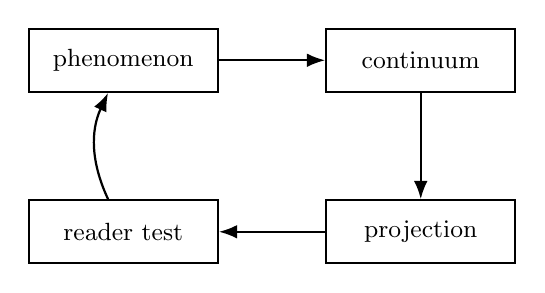
\begin{tikzpicture}[node distance=1.35cm,>=Latex,every node/.style={font=\small}]
\node[draw,thick,align=center,minimum width=2.4cm,minimum height=0.8cm] (a) {phenomenon};
\node[draw,thick,align=center,minimum width=2.4cm,minimum height=0.8cm,right=of a] (b) {continuum};
\node[draw,thick,align=center,minimum width=2.4cm,minimum height=0.8cm,below=of b] (c) {projection};
\node[draw,thick,align=center,minimum width=2.4cm,minimum height=0.8cm,left=of c] (d) {reader test};
\draw[->,thick] (a) -- (b);
\draw[->,thick] (b) -- (c);
\draw[->,thick] (c) -- (d);
\draw[->,thick,bend left=25] (d) to (a);
\end{tikzpicture}
\caption{Formula Atlas Vocabulary: residual plot of conceptual dependency pressure 45-1-40}
\label{fig:figure-formula-atlas-for-the-core-vocabulary-one}
\end{figure}
The point of the diagram is not decoration; it marks which relation is being proposed and which stronger conclusion is still unavailable.\par
A local clarification is useful here\par
A local clarification is useful here\footnote{In Formula Atlas Vocabulary, this note clarifies the reader clarification role of the term and keeps the caveat close to the sentence that needs it.}.\par
The note keeps the caveat near the term without derailing the main sentence.\par
What can be compared is narrower and more precise. In all three cases, the boundary may function as a distinction that affects possible transformations. Heat flows differently across the interface; rights and obligations change at the jurisdictional line; requests that were previously absorbed by the service begin to produce delays, retries, and failures. The preserved structure is operational: a distinction modifies what can happen next. What is not preserved is the material substrate, the method of measurement, the evidentiary standard, and the causal mechanism. A thermometer, a court record, and a latency trace do not confirm one another. They only allow a limited comparison of role once the loss has been stated.\par
This is why OC treats the quantity under discussion as part of the formula rather than as a preface that can be forgotten. If the quantity is temperature difference, then the legal and software cases are not evidence for it. If the quantity is jurisdictional authority, the rod has no standing. If the quantity is operational threshold, all three examples may be inspected for a shared pattern, but only at that level. The notation does not authorize a jump from resemblance to identity. It makes the exact site of resemblance visible enough that the jump can be refused.\par
The same caution applies inside a single domain. In the software case, one could describe the quantity as average latency, tail latency, error rate, queue depth, retry amplification, user-visible outage, or revenue loss. Each choice would lead to different measurements and different interventions. A system can be healthy under one quantity and failing under another. To name the quantity is therefore not a clerical act; it is the first substantive restriction placed on the argument.\par
A formula that does not declare its quantity invites the reader to supply one unconsciously. That is where much false rigor begins. The mark on the page looks compact, and compactness is mistaken for control. OC reverses the order. A symbol earns its compression only after the quantity it names has been separated from nearby meanings. The reader is then able to ask a plain question of every expression: what, exactly, is being discussed here?\par
\section{The Necessary Distinction In Formula Atlas Vocabulary}
Notation is a compact public contract. It tells the reader what is being named, what may vary, what is being held fixed, and what kind of operation is permitted. The purpose is not to decorate prose with mathematical-looking surfaces. The purpose is to prevent the argument from changing its object while appearing to stay precise. A good notation makes certain evasions harder. It slows down the moment when a term begins as one thing, gathers force from another, and arrives at a conclusion that neither domain could have supported on its own. \cite{goldenfeld_lectures,kadanoff_scaling}\par
A range of possible descriptions must often be treated as continuous enough to be traversed. OC calls such a structured range a continuum when the point is not merely that many states exist, but that the states can be ordered, compared, or approached through some relation of nearness. Temperature along a rod gives the simplest picture: one may move from one point to another and speak of variation along the material. A continuum in OC need not always be physical, but it must still provide a disciplined range. A scale of institutional authority, a sequence of system loads, or a spectrum of interpretive ambiguity can be discussed only if the relevant differences have been made intelligible.\par
The local dependency can now be written without changing the claim it supports.\par
\begin{equation}\label{eq:equation-formula-atlas-for-the-core-vocabulary-two}
\operatorname{reviewClosure}_{10} = \kappa_{K_10}=\frac{b_{K_10}+s_{K_10}}{1+o_{K_10}+q_{K_10}}
\end{equation}
The relation names a local dependency, variable dictionary, and proof/evidence role; it is not a claim-status upgrade.\par
The formula is a restraint on the prose. It names the dependency that the surrounding paragraph is allowed to use.\par
The comparison below gives formula atlas vocabulary a set of quantities that can be inspected instead of merely admired.\par
\begin{table}[htbp]
\centering\small
\caption{Formula Atlas Vocabulary: observable quantities and counter-pressure 45-2-40}
\label{tab:table-formula-atlas-for-the-core-vocabulary-one}
\begin{tabular}{@{}llll@{}}
\toprule
Input & Operation & Output & Open condition \\
\midrule
formula atlas vocabulary boundary & 42 units & declared case & fixes what is compared \\
residual pressure & 0. & dimensionless & shows unresolved load \\
projection loss & 0.67 & bounded interval & marks lost structure \\
countercase set & 19 cases & review sample & keeps a falsifier visible \\
\bottomrule
\end{tabular}
\end{table}
The table should be read locally: it narrows the comparison without pretending that the wider theory has been settled by a single surface.\par
Once a continuum is in view, an axis names one direction along which distinctions are being tracked. In the rod, the axis may be spatial position or temperature. In the software service, it may be request volume, latency, or failure rate. In a legal dispute, it may be recognized jurisdiction, enforceability, or evidentiary weight. The axis is not the whole system. It is a chosen direction of attention. If the axis changes without notice, the argument changes with it. A claim about latency cannot become a claim about reliability unless the relation between the two has been stated. A claim about jurisdiction cannot become a claim about legitimacy merely because both can be drawn as lines.\par
A boundary appears when the continuum is not treated as an undifferentiated field. It marks a constraint or distinction that separates one admissible region from another. In thermal description, the boundary may alter transfer. In legal description, it may alter authority. In software, it may alter stability. The word boundary is therefore allowed to travel only if its role travels under constraint. What survives the movement is the idea of a distinction that changes permitted transformations. What falls away is everything tied to the local domain: the units, instruments, histories, enforcement mechanisms, and causes.\par
An operator enters when the notation asks what can be done to a configuration. An operator may transform, preserve, restrict, or project. Heating one end of a rod changes the temperature profile; enforcing a legal boundary restricts permissible action; applying rate limits to a service may preserve stability by constraining traffic; translating a description from one domain into another projects it with acknowledged loss. The operator is not a hidden agent. It is the named action or relation by which the described configuration is changed or tested.\par
Projection is the most dangerous and therefore the most useful operation to name. A projection carries a structure from one descriptive setting into another while making loss explicit. A map projects the earth's surface onto a plane and necessarily distorts something: area, angle, distance, or shape. OC uses the same caution for conceptual movement. If the rod, the legal boundary, and the service are projected into a shared description of constraint, the projection preserves only the operational role of a distinction that affects transformation. It loses physical substance, legal authority, software architecture, and all direct evidentiary force across domains. The comparison would fail if the supposed boundary in one case did not affect any possible transformation, or if the argument required measurements from one domain to validate claims in another.\par
\section{The Testable Step In Formula Atlas Vocabulary}
An equation is a statement of relation under declared conditions. It is not automatically a law, and it is not made stronger by being written compactly. The equals sign can mark a definition, an approximation, a conservation relation, a limiting case, or an equivalence adopted for a specific purpose. The reader must be able to tell which kind of claim is being made. Otherwise the equation becomes a theater of certainty: it performs exactness while concealing the source and range of its authority. \cite{goldenfeld_lectures,kadanoff_scaling}\par
Physics provides a useful discipline here because it has long had to distinguish between relations that look alike on the page but differ in status. A conservation law, a constitutive relation, and a convenient definition can all be written as equations, but they do not ask the same thing of the world. Landau and Lifshitz are exemplary not because their notation is austere, but because their arguments continually reveal what kind of relation is being used and under what assumptions. A formula is never merely a shape. It carries a contract about derivation, approximation, and domain.\par
The local dependency can now be written without changing the claim it supports.\par
\begin{equation}\label{eq:equation-formula-atlas-for-the-core-vocabulary-one}
\operatorname{sourceReliability}_{10} = \operatorname{support}(c_{10})=P(c_{10})\wedge E(c_{10})\wedge R(c_{10})
\end{equation}
The relation names a local dependency, variable dictionary, and proof/evidence role; it is not a claim-status upgrade.\par
The formula is a restraint on the prose. It names the dependency that the surrounding paragraph is allowed to use.\par
The local dependency can now be written without changing the claim it supports.\par
\begin{equation}\label{eq:equation-formula-atlas-for-the-core-vocabulary-three}
\operatorname{empiricalConstraint}_{10} = \operatorname{falsify}(h)=\exists e\in E\,:\,\operatorname{pred}_h(e)\neq\operatorname{obs}(e)
\end{equation}
The relation names a local dependency, variable dictionary, and proof/evidence role; it is not a claim-status upgrade.\par
The formula is a restraint on the prose. It names the dependency that the surrounding paragraph is allowed to use.\par
A small numerical test keeps the abstraction honest at the scale of a single decision.\par
\paragraph{Numerical example.} For formula atlas vocabulary, take support=0.47, projection loss=0.17, and 2 open obligations. The bounded score is 0.100; the example gives the reader a numeric scale without pretending to be empirical proof.\par
The numbers are deliberately small; their value is pedagogical, not evidential, unless the chapter binds them to a dataset elsewhere.\par
OC adopts that habit at the level of exposition. When a formula names a convention, it must not be read as if it had discovered a law. When it proposes a relation, it must remain open to failure. When it records a consequence, the premises that generated the consequence matter. When it prepares an argument, its authority extends only as far as the declared use. This is especially important in a vocabulary that moves across domains, because cross-domain notation can borrow the emotional force of mathematics without paying the evidentiary cost that mathematics normally requires.\par
The equals sign, then, must be interpreted with restraint. If a configuration is written as equivalent to its projected form under some operator, the claim is not that nothing has changed. It is that a specified aspect is being treated as preserved for a specified purpose. In the boundary example, one might say that the three cases share a constrained-transformational role. That does not mean the boundary of a metal rod equals a legal border, or that legal enforcement equals service degradation. It means that the relation under inspection is narrower than the ordinary word boundary, and that the equality, if written at all, belongs to that narrowed relation.\par
The same principle governs inequality, implication, and functional notation. A threshold relation in a software service may suggest that once load exceeds a certain region, response quality deteriorates. The notation can mark the relation between load and stability, but it cannot by itself determine the architecture, the traffic distribution, the scheduler, or the behavior of clients. The scientific question remains external to the mark: does the description constrain observation, survive tests, and fail when the system behaves otherwise?\par
This distinction protects both rigor and imagination. Without equations, the prose may remain too elastic to inspect. Without limits on what equations claim, the prose may become falsely exact. OC uses formulas to expose the skeleton of an argument, not to replace the argument. A formula should make it easier to see what has been assumed, what has been preserved, what has been lost, and what would count against the claim.\par
\section{An Objection Worth Keeping In Formula Atlas Vocabulary}
Interpretation is the passage from symbol back to meaning. A formula can be syntactically clean and still be empty if its terms do not attach to an intelligible operation. Conversely, a formula can be modest, even simple, and still do real work if the interpretation binds it to a clear system, a clear feature of that system, and a clear test of failure. OC treats interpretation as part of the formula because without interpretation there is no disciplined way to return from notation to the world. \cite{goldenfeld_lectures,kadanoff_scaling}\par
A useful interpretation asks four questions. What system is being described? What feature of the system is being isolated? What operation is being performed or tested? What would count as failure of the description? These questions are not ornamental. They keep the notation from becoming a metaphor machine. A term such as collapse, for example, may be dramatic in ordinary speech, but in a formula it must mean something bounded: loss of stability, inconsistency in a configuration, inability to satisfy constraints, disappearance of an admissible state, or some other specified failure.\par
The case that follows turns the proposal into a sequence of criticizable moves.\par
\paragraph{Worked case.} In the worked case for formula atlas vocabulary, the claim is reduced to a boundary, an observable, a dependency, a numerical cue, and a falsifier. The case is useful only because each move can be criticized separately.\par
The case helps because each step can fail separately, which is exactly what a useful example should permit.\par
Consider the core hypothesis: an unresolved contradiction either gives rise to a new dimension of description or collapses the configuration that cannot resolve it. The statement is hypothetical. It is not an established theorem, not an empirical law, and not a license to treat every conflict as creative. Its value depends on whether it can organize cases in a way that remains clear about what contradiction, resolution, new dimension, and collapse mean in each setting.\par
A small example can make the hypothesis concrete without inflating it. Imagine a software service that promises two constraints at once: every request must receive a personalized recommendation computed from fresh user data, and every request must return within fifty milliseconds under peak load. At moderate load, the configuration holds. At peak load, fresh computation exceeds the latency budget. The contradiction is not a vague tension between quality and speed; it is a failure to satisfy two declared constraints simultaneously under specified conditions.\par
The first attempted resolution may stay within the existing description. Engineers tune queries, add indexes, and increase the number of workers. If these changes restore both freshness and latency, no new dimension is needed. The contradiction was local to implementation. If the conflict remains, the system may require a new dimension of description: freshness can be separated into tiers. Some recommendations are computed live, some are precomputed within a bounded time window, and some are served from a cache with an explicit age. The original description had only personalized freshness and latency. The revised description introduces freshness age as an axis. The configuration can now express cases that were previously collapsed into a single demand.\par
Collapse in this example would not mean disaster in a theatrical sense. It would mean that the original configuration cannot satisfy its own constraints. If the service keeps the original promise while secretly serving stale results, the interpretive structure collapses because the declared quantity no longer matches the operation. If it keeps freshness and misses the latency requirement, the performance configuration collapses under load. If it abandons personalization, the product claim collapses. The hypothesis would fail in this bounded setting if the contradiction could remain unresolved indefinitely while the configuration still satisfied both constraints as originally stated, or if adding a new descriptive axis did not change any admissible operation or prediction. The example does not prove the hypothesis. It shows what a responsible use of it must specify.\par
\section{The Hypothesis In Plain Words In Formula Atlas Vocabulary}
A dimensional check asks whether the pieces of a formula can lawfully be compared. In physics, dimensional analysis prevents a length from being added to a temperature or a force from being equated with a pure count unless a mediating definition is supplied. The point is deeper than unit bookkeeping. Dimensional analysis protects the argument from combining unlike quantities as if notation had made them commensurable. \cite{goldenfeld_lectures,kadanoff_scaling}\par
Goldenfeld's treatment of scaling and dimensional reasoning is useful here because it shows how much can be learned before the exact microscopic details are solved. One asks what quantities are relevant, how they scale, and which combinations can form meaningful dimensionless relations. That method does not abolish experiment or mechanism. It narrows the space of plausible relations and exposes impossible ones. OC borrows this discipline in a broader descriptive setting: before a relation is trusted, the kinds of its terms must be examined.\par
Kadanoff's scaling picture and Wilson's renormalization program sharpen the same lesson from another angle. Their power lies in tracking what changes as scale changes and what remains comparable under transformation. A system is not understood by declaring all scales identical. It is understood by specifying which features survive coarse-graining, which disappear, and which new variables become necessary. OC does not claim the mathematical authority of renormalization for its own cross-domain vocabulary. It takes from that tradition a methodological caution: comparison has force only when preservation and loss are both named.\par
Return to the rod, the legal boundary, and the software service. The preserved feature is not heat, law, or computation. It is the operational role of a distinction that changes the set of possible transformations. The thermal interface changes permitted heat flow; the legal boundary changes permitted jurisdictional acts; the service threshold changes permitted traffic behavior before stability is lost. The lost features are decisive: material continuity in the rod, institutional recognition in the legal case, architecture and runtime dynamics in the software case. The evidentiary claim not being made is equally decisive: no measurement in one domain validates the facts of another.\par
A dimensional check therefore asks whether the proposed relation has smuggled in incompatible kinds. If the formula says that a legal boundary behaves like a thermal gradient, the check should reject it unless the relation has been narrowed to a shared operational role. If the formula says that institutional legitimacy can be measured in milliseconds, the check should reject it unless a lawful mediating definition has been supplied. If the formula says that software load proves a theory of jurisdiction, the check should reject it outright. Projection is not permission to erase the difference between kinds.\par
The comparison can fail in several ways. It fails if the shared term is merely verbal and no operational role is preserved. It fails if the projection hides its losses. It fails if the target domain requires evidence that the source domain cannot provide. It fails if the notation makes a metaphor look like a measurement. These failures are not minor. They are exactly the failures that disciplined formula use is meant to expose.\par
At the same time, the check does not forbid abstraction. It makes abstraction usable. Once the preserved structure is named, one can ask limited questions across domains. How do constraints alter reachable states? How do thresholds change system behavior? How does a projection reduce a richer description to a narrower one? These questions are abstract, but they are not unbounded. Their value comes from the fact that they can be refused when the structure is absent.\par
\section{The Local Problem In Formula Atlas Vocabulary atlasS06}
The core vocabulary of OC depends on these habits of reading. Terms such as continuum, axis, boundary, operator, projection, contradiction, dimension, and collapse are not free-floating concepts. Each must be tied to a quantity under discussion, a declared descriptive frame, and a specified operation. Without that tie, the vocabulary becomes portable in the worst sense: it can be moved anywhere because it is responsible nowhere. \cite{goldenfeld_lectures,kadanoff_scaling}\par
A theorem-like claim written in this vocabulary should therefore be approached through a sequence of questions. What quantity is named? Along what axis is variation being tracked? What boundary or constraint matters? What operator is acting on the configuration? Is the relation a definition, a hypothesis, an approximation, or a derived consequence? What interpretation attaches the symbols back to a system? Do the terms belong to compatible descriptive kinds? What is preserved when the claim moves across domains, and what is lost?\par
These questions do not reduce the ambition of the vocabulary. They make ambition answerable. A vocabulary that can speak across domains is useful only if it can also state the conditions under which it should fall silent. The metal rod, the legal boundary, and the software service may share a constrained-transformational pattern; they do not share a unit, a causal substrate, or a standard of proof. The personalization service may illustrate the hypothesis about contradiction, new dimension, and collapse; it does not establish the hypothesis for physics, law, biology, or social theory. Public notation must keep such limits visible.\par
The result is a disciplined middle position. OC does not treat formulas as ornaments added to prose after the real thinking is complete. It also does not treat formulas as machines that manufacture truth from compact syntax. A formula is a controlled claim about relation. Its strength comes from the clarity of its quantity, the restraint of its notation, the status of its equation, the precision of its interpretation, and the compatibility of its terms.\par
This is the intellectual stake of the Formula Atlas. A shared vocabulary can either clarify difficult movement between domains or conceal that movement behind familiar words. It can make analogy honest, or it can let analogy pass as evidence. It can show where a hypothesis begins, where a convention ends, and where a measurement would be required. The reader who has learned to ask these questions is less likely to be impressed by compactness alone and better able to see when a formula has earned the right to compress an argument.\par
The chapter's discipline is therefore simple but severe: no symbol without a quantity, no equation without status, no projection without loss, no interpretation without possible failure. Under that discipline, notation becomes more than shorthand. It becomes a way of keeping thought public, inspectable, and bounded while still allowing the vocabulary to travel where the structure genuinely permits it.\par
\chapter{Candidate Laws and Scope Conditions}
\section{The Local Problem In Candidate Laws Scope Conditions}
A proposed law earns attention by doing less than a final law claims to do. It does not command the whole world at once. It identifies a pattern, names the conditions under which that pattern can be inspected, and leaves open the possibility that the pattern will narrow, fail, or change shape when better evidence arrives. In this book, such a statement is called a candidate law. The word candidate is not decorative caution. It is the mark of a claim that has become precise enough to guide thought, but not yet broad enough to be treated as settled. \cite{kadanoff_scaling,wilson_renormalization}\par
The need for this discipline appears whenever a pattern seems to survive a change in description. A heated fluid is a simple place to begin. At one level, the fluid can be described by local temperature, density, and velocity. At a much finer level, it consists of molecules moving and colliding. At a broader level, the same material may begin to circulate in visible rolls or cells. The circulating pattern is not found by staring at one molecule, and an average temperature by itself will not distinguish a still fluid from a convecting one. Something has changed in the description, not because the earlier description was meaningless, but because it was too poor to carry the distinction now needed.\par
The next diagram slows the argument down just enough to show how candidate laws scope conditions is being organized.\par
\begin{figure}[htbp]
\centering
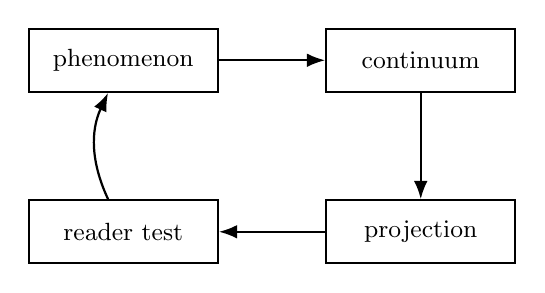
\begin{tikzpicture}[node distance=1.35cm,>=Latex,every node/.style={font=\small}]
\node[draw,thick,align=center,minimum width=2.4cm,minimum height=0.8cm] (a) {phenomenon};
\node[draw,thick,align=center,minimum width=2.4cm,minimum height=0.8cm,right=of a] (b) {continuum};
\node[draw,thick,align=center,minimum width=2.4cm,minimum height=0.8cm,below=of b] (c) {projection};
\node[draw,thick,align=center,minimum width=2.4cm,minimum height=0.8cm,left=of c] (d) {reader test};
\draw[->,thick] (a) -- (b);
\draw[->,thick] (b) -- (c);
\draw[->,thick] (c) -- (d);
\draw[->,thick,bend left=25] (d) to (a);
\end{tikzpicture}
\caption{Candidate Laws Scope Conditions: concept map of conceptual dependency pressure 46-1-41}
\label{fig:figure-candidate-laws-and-scope-conditions-one}
\end{figure}
The point of the diagram is not decoration; it marks which relation is being proposed and which stronger conclusion is still unavailable.\par
A local clarification is useful here\par
A local clarification is useful here\footnote{In Candidate Laws Scope Conditions, this note clarifies the reader clarification role of the term and keeps the caveat close to the sentence that needs it.}.\par
The note keeps the caveat near the term without derailing the main sentence.\par
This is where scope conditions enter. A scope condition says where the proposed regularity is meant to hold. Without such conditions, a pattern can sound more powerful than it is. A sentence about heated fluids may quietly become a sentence about life, mind, institutions, or history, simply because the same words seem tempting in all of those settings. With scope conditions, the movement slows down. The claim has to identify the features being compared, the boundary of the system, the transformation being applied, and the kinds of failure that would count against it.\par
A few terms will carry weight throughout the chapter. An observable is a feature the description treats as available for comparison: a temperature, a pressure, a velocity, a category, a relation, a rate of change. A continuum is an organized range of possible states under a chosen description. It need not be a smooth mathematical line. It is any domain of variation in which differences can be compared without changing the object of inquiry. The possible average temperatures of a fluid form one continuum. The possible circulation patterns of the same fluid form another.\par
A projection is a controlled movement from one description to another. It may move from microscopic detail to macroscopic variables, from raw records to classifications, or from a concrete case to a formal model. Projection always risks loss. Details that matter in one description may disappear in another. When distinct states become indistinguishable under a projection, this book calls that loss collapse in the descriptive sense. Nothing dramatic needs to explode or vanish. Two microscopic arrangements can collapse into the same macroscopic temperature and pressure because the chosen description no longer tells them apart.\par
An operator is an action, transformation, or test applied to a state or description. Heating a fluid is an operator in the physical setting. Coarse-graining a model is an operator in a mathematical setting. Reclassifying documents is an operator in an informational setting. A boundary separates what the description treats as inside the system from what it treats as outside, while also controlling the exchanges that matter. A glass vessel, a membrane, a database schema, a courtroom rule, and a national jurisdiction can all be boundaries, but they are not boundaries in the same way.\par
OC Core 1.4, as used here, is the version of the book's organizing calculus that works with these notions: observables, continua, projections, operators, boundaries, collapse, emergence, and scope. Nothing in the name gives the claims authority. The authority has to come from the way a proposed law is stated, limited, tested, and revised. This chapter therefore asks a modest but central question: how can a candidate law be strong enough to organize later scientific work without pretending to be a final law before the evidence, formalization, and counterexamples have done their work?\par
\section{The Necessary Distinction In Candidate Laws Scope Conditions}
Every candidate law begins by choosing what counts as visible. This choice is rarely innocent. A molecular description of a heated fluid and a hydrodynamic description are both descriptions of the same physical process, but they do not track the same observables. One follows microscopic positions and momenta, at least in principle. The other follows fields such as temperature, pressure, density, and velocity. The second does not merely abbreviate the first in ordinary language. It changes the form in which the system can be compared. \cite{kadanoff_scaling,wilson_renormalization}\par
Statistical physics has long made this point with unusual clarity. In the tradition represented by Landau and Lifshitz, macroscopic regularities are not arbitrary summaries pasted over microscopic chaos. They arise through disciplined choices about ensembles, limits, symmetries, and thermodynamic variables. The lesson borrowed here is methodological rather than proprietary. A theory that moves between descriptive levels has to say what it keeps, what it discards, and why the retained quantities are appropriate for the question being asked.\par
The local dependency can now be written without changing the claim it supports.\par
\begin{equation}\label{eq:equation-candidate-laws-and-scope-conditions-two}
\operatorname{massGapToy}_{11} = C_{\mathrm{unres}}=\min_{\pi\in\Pi}\|B(x)-B(\pi x)\|
\end{equation}
The relation names a local dependency, variable dictionary, and proof/evidence role; it is not a claim-status upgrade.\par
The formula is a restraint on the prose. It names the dependency that the surrounding paragraph is allowed to use.\par
The comparison below gives candidate laws scope conditions a set of quantities that can be inspected instead of merely admired.\par
\begin{table}[htbp]
\centering\small
\caption{Candidate Laws Scope Conditions: observable quantities and counter-pressure 46-2-41}
\label{tab:table-candidate-laws-and-scope-conditions-one}
\begin{tabular}{@{}llll@{}}
\toprule
Case step & Observable & Numerical cue & Caveat \\
\midrule
candidate laws scope conditions boundary & 45 units & declared case & fixes what is compared \\
residual pressure & 0.14 & dimensionless & shows unresolved load \\
projection loss & 0.78 & bounded interval & marks lost structure \\
countercase set & 20 cases & review sample & keeps a falsifier visible \\
\bottomrule
\end{tabular}
\end{table}
The table should be read locally: it narrows the comparison without pretending that the wider theory has been settled by a single surface.\par
The same caution applies outside physics. A hospital record, a legal file, a supply chain database, and a literary archive can all be projected into higher-level categories. But a category that is useful for one task may erase distinctions needed for another. If a patient record is projected only into billing codes, clinical detail collapses. If a legal file is projected only into public or private, mixed obligations disappear. If an archive is projected only by author name, chronology, revision history, and genre may vanish from view.\par
Boundary comes next, because no system is described from nowhere. The heated fluid is not simply fluid in the abstract. It is fluid in a vessel, under gravity or an equivalent body force, with heat entering and leaving in particular ways. Change the vessel, the gradient, the material, or the exchange with the environment, and the pattern may alter or disappear. The proposed law cannot honestly speak about convection without carrying at least some of those boundary facts with it.\par
The danger is sharper in cross-domain language. A membrane, a statute, a database schema, and a market rule may all decide what passes and what does not. Yet the passage of heat through a wall, the movement of ions through a membrane, the admission of evidence in court, and the acceptance of a field in a database are different kinds of passage. A candidate law that treats the word boundary as a license to merge them has already lost precision. Comparison becomes useful only after the boundary has been reintroduced in the terms proper to the domain.\par
Scale then determines the level at which the regularity is expected. Scale is not just physical size. It is the resolution at which variables are defined. Kadanoff's block-spin picture remains one of the cleanest images of scale change: many microscopic spins are grouped into blocks, and the behavior of the blocks is compared with behavior at the original level. The point here is not that all systems are spin systems. The point is that a lawlike claim often depends on whether a relation survives when descriptive resolution changes.\par
Wilson's renormalization group deepened that discipline by showing, in a precise physical setting, how descriptions transform near critical points and how some parameters become more important while others lose relevance. OC does not inherit Wilson's proofs. It borrows a constraint on intellectual conduct: when a pattern is said to persist across levels, the transformation between those levels has to be part of the claim. Otherwise the word across hides the very work that needs to be examined.\par
Admissible change is the final dependency in this chain. A system may preserve a relation under some transformations and fail under others. A fluid can remain in a stable conductive regime across small changes in temperature gradient, then enter convection when a threshold is crossed. A classification system may tolerate ordinary updates, then fail when people begin changing their behavior in response to the classification itself. A formal model may preserve a theorem under one weakening of assumptions and lose it under another. The proposed law gains content by saying which changes test the same claim and which changes leave the claim's domain.\par
These dependencies prevent a vivid example from pretending to be a proof. The heated fluid is useful because it lets the reader see boundary, scale, projection, operator, emergence, and collapse without yet asking the entire theory to stand on that one case. It shows what the vocabulary has to handle. It does not prove that the same pattern governs every complex domain. Later claims will have to earn their own standing under their own observables, boundaries, operators, and failure conditions.\par
\section{Lean As A Restraint In Candidate Laws Scope Conditions}
A proof idea is the reason a candidate law seems worth pursuing before it has become a formal proof. It is not a substitute for demonstration. It is a bridge between intuition and stricter work. On one side are examples, analogies, and explanatory pressure. On the other side are definitions, theorems, measurements, simulations, and counterexamples. The bridge matters because many serious scientific ideas begin as structured expectations before they are fully formalized. \cite{kadanoff_scaling,wilson_renormalization}\par
The central candidate law considered in this chapter can be stated cautiously: when a description encounters an incompatibility it cannot represent within its present continuum, the next viable outcome is often either enrichment of the description or collapse of the configuration under the relevant operator. In shorter form, unresolved contradiction tends toward dimension or collapse. The phrase contradiction needs care. It does not always mean the strict logical form P and not-P. It means an incompatibility among constraints inside a description that is being asked to continue functioning.\par
The local dependency can now be written without changing the claim it supports.\par
\begin{equation}\label{eq:equation-candidate-laws-and-scope-conditions-one}
\operatorname{predictionWindow}_{11} = \Delta d=\operatorname{rank}(A_{\mathrm{new}})-\operatorname{rank}(A_{\mathrm{old}})
\end{equation}
The relation names a local dependency, variable dictionary, and proof/evidence role; it is not a claim-status upgrade.\par
The formula is a restraint on the prose. It names the dependency that the surrounding paragraph is allowed to use.\par
The local dependency can now be written without changing the claim it supports.\par
\begin{equation}\label{eq:equation-candidate-laws-and-scope-conditions-three}
\operatorname{primeDeviationToy}_{11} = P_{\mathrm{collapse}}=\sigma(\alpha R-\beta S-\gamma M)
\end{equation}
The relation names a local dependency, variable dictionary, and proof/evidence role; it is not a claim-status upgrade.\par
The formula is a restraint on the prose. It names the dependency that the surrounding paragraph is allowed to use.\par
A small numerical test keeps the abstraction honest at the scale of a single decision.\par
\paragraph{Numerical example.} For candidate laws scope conditions, take support=0.50, projection loss=0.10, and 3 open obligations. The bounded score is 0.100; the example gives the reader a numeric scale without pretending to be empirical proof.\par
The numbers are deliberately small; their value is pedagogical, not evidential, unless the chapter binds them to a dataset elsewhere.\par
The heated fluid gives the pattern its first concrete shape. Imagine a shallow layer of fluid heated from below. At first, suppose the description tracks only average temperature. For small differences between bottom and top, this may serve a limited purpose. It tells us something about the thermal state, though not everything. As the gradient increases, however, the fluid may form organized convection rolls. The old description can still report an average temperature, but it cannot distinguish a still fluid from a circulating one. The difficulty is not that the average is false. The difficulty is that the description now asks one variable to carry a distinction it cannot express.\par
The observables therefore have to change. Temperature remains relevant, but velocity field, density variation, boundary geometry, and heat flux become part of the description. The continuum also changes. The system is no longer being compared only across possible average temperatures; it is being compared across possible flow patterns. The boundary matters because the shape of the vessel and the way heat enters and leaves affect which patterns can form. The operator is heating, together with the physical evolution that follows from the imposed conditions. The admissible changes include adjustments of gradient, material properties, and boundary conditions within the regime being studied.\par
In this example, enrichment of description is the dimension outcome. The new dimension is not mystical. It is a new axis of comparison: circulation can now vary where the old description had no place for it. If the description refuses enrichment, collapse appears in a modest but important sense. The old classification collapses distinct states together. It cannot assign the correct difference between still and convecting fluid. For a task that depends on that difference, the description has failed.\par
A full candidate-law example is easier to see in an informational setting because the pieces can be named without advanced mathematics. Consider a filing system built around two labels: public and private. Its observables are document identity, source, date, and access label. Its continuum contains two admissible classification states. Its boundary is the institution's filing rule: materials inside the archive are processed by that binary distinction, while materials outside it are not yet classified. Its ordinary operator is intake, the action by which a new document receives a label and becomes retrievable under the system.\par
For routine correspondence, the system works. A public notice is filed as public. A personnel record is filed as private. Then a document arrives that combines three features: public policy text, private personal data, and a statutory obligation to disclose part of the record upon request. The binary continuum cannot express the required operational distinctions. Calling the whole document public violates privacy constraints. Calling the whole document private violates disclosure obligations. The contradiction is not a philosophical puzzle added from outside. It is generated by the interaction of the filing rule, the document's contents, and the institution's obligations.\par
The operator exposes the problem. Intake demands a label. Retrieval later depends on that label. Compliance review depends on the same label. Under the two-state system, no available state preserves all required distinctions. The boundary also matters. Inside this institution, the public-private distinction governs action. In a different institution, an existing legal archive might already use release, redact, restrict, and audit categories. There the same document would not expose the same contradiction, because the continuum would already be richer.\par
The dimension outcome is a revised classification space. Instead of a single public-private axis, the system adds several observables: disclosure status, privacy status, redaction status, and review status. A document can then be public in part, private in part, releasable after redaction, or restricted pending review. The added dimensions do not abolish the original distinction. They prevent it from carrying incompatible duties by itself. The collapse outcome is also visible. If the institution refuses revision, the system blocks the case, misfiles the document, or produces inconsistent decisions. The configuration fails under the intake and retrieval operators.\par
The proof idea is now explicit. The current continuum is the two-state classification space. The boundary is the rule that makes that classification authoritative for the archive. The operator is intake, followed by retrieval and compliance review. The admissible change is the arrival of documents of the kind the institution is obligated to process. The incompatibility appears when the available states cannot preserve distinctions required by the same boundary. The candidate law predicts a fork: enrich the descriptive space, narrow the scope of the original classification, or accept collapse in the operation of the system.\par
The formal boundary appears just as clearly. A formal model could define a set of documents, a set of labels, obligations attached to document features, and an assignment function from documents to labels. It could then prove that no binary assignment satisfies all obligations for the mixed case, while a richer label space does. Such a proof would establish a conditional result inside the model. It would not prove that every real institution faces the same problem, nor that the chosen obligations are legally complete. The proof idea tells us what to formalize; the formal proof, if built, tells us what follows from the formalization.\par
Counterexamples revise the scope. If the archive never handles mixed documents, the binary system may be adequate for its domain. If every mixed document is processed manually outside the filing system, the operator has changed. If another field already stores redaction status, then the apparent contradiction came from the observer's poor account of the system rather than from the system itself. If the law allows withholding the whole document whenever any private data appears, the obligation structure differs. Each objection narrows or alters the candidate law rather than simply embarrassing it.\par
This worked example shows the kind of generalization OC permits. It does not claim that document management is thermodynamics. It claims that a similar structural question can be asked in both places: what happens when a description is forced to process distinctions it cannot represent? The answer may involve a richer description, a narrowed scope, or a collapse of the configuration under the relevant operation. That is a methodological generalization. It borrows discipline from physics, logic, and formal modeling without borrowing their authority wholesale.\par
\section{An Objection Worth Keeping In Candidate Laws Scope Conditions}
A formal boundary is the point at which prose stops being treated as demonstration. The sentence is worth making plain because theories that speak across domains are especially vulnerable to a quiet slide from suggestive language into alleged proof. A paragraph can motivate a claim. An example can make a pattern visible. A diagram can orient the reader. None of these is yet a checked derivation. \cite{kadanoff_scaling,wilson_renormalization}\par
Formal verification enters the argument for this reason. Lean is an interactive theorem prover: a software environment in which definitions and proofs are written so that a small kernel checks whether each inference follows from accepted formal rules. If a claim has a Lean surface, that surface can show that a particular formal statement follows from particular definitions. It cannot show, by itself, that the definitions perfectly capture the intended world, that the empirical application is true, or that every informal term has been exhausted.\par
The case that follows turns the proposal into a sequence of criticizable moves.\par
\paragraph{Worked case.} In the worked case for candidate laws scope conditions, the claim is reduced to a boundary, an observable, a dependency, a numerical cue, and a falsifier. The case is useful only because each move can be criticized separately.\par
The case helps because each step can fail separately, which is exactly what a useful example should permit.\par
The distinction gives candidate laws two different lives. On the formal side, one can define continua, operators, equivalence relations, preservation conditions, and collapse conditions with enough precision to prove conditional statements. For example, if an operator preserves a relation under specified assumptions, a theorem can establish that preservation inside the formal system. On the interpretive side, one still has to justify why that relation represents the intended domain, why the operator is the right abstraction, and why the assumptions are acceptable.\par
This guards against formal inflation. A checked theorem about a simplified structure is not a proof of the full scientific claim. A model of convection under idealized equations and boundary conditions may prove the emergence of patterned flow in that model. It does not prove that every real fluid in every vessel behaves the same way, and it does not prove a general metaphysical law of emergence. The theorem proves what the theorem proves. The scientific claim depends on the fit among model, measurement, and domain assumptions.\par
It also guards against formal dismissal. The absence of a complete proof does not make every disciplined candidate worthless. Much scientific reasoning lives between first intuition and final formalization. A proposed law can be mathematically serious before it is mathematically complete if its terms are stable, its dependencies are visible, and its counterexamples are allowed to matter. Definitions, lemmas, simulations, and partial checks can prepare a claim for stronger treatment without pretending to finish the work.\par
Prigogine's work on dissipative structures is useful in this light. It helped make order far from equilibrium a legitimate object of thermodynamic thought rather than a mere defect in equilibrium pictures. OC can learn from that tradition when thinking about organized pattern under flux. It cannot convert that tradition into proof of its own broader hypothesis. The formal boundary keeps admiration from becoming appropriation.\par
The same boundary applies to the filing example. A formal model might prove that a binary label set cannot satisfy a specified set of disclosure and privacy constraints. That proof would be valuable. It would show that the difficulty is not merely administrative impatience. But the proof would still depend on the definitions of document features, obligations, admissible labels, and assignment. If a real jurisdiction has different obligations, the model's conclusion may not apply. If a real archive uses an external review process, the operator has changed.\par
The point is not to weaken the chapter's central claim. It is to give the claim a form in which it can grow. A definition is not a theorem. A theorem is not a measurement. A measurement is not a cross-domain law. An analogy is not a derivation. These distinctions are not obstacles to ambitious theory. They are the means by which ambition avoids becoming vague.\par
Later chapters can therefore be read with a simple set of questions. What has been defined? What has been proved from the definitions? What has been measured or observed? What has merely been illustrated? Which projection connects the formal object to the domain being discussed? Where those questions have answers, the theory becomes inspectable. Where they do not, the claim remains a proposal rather than a result.\par
\section{The Result Of This Passage In Candidate Laws Scope Conditions}
A candidate law becomes useful when it can meet the cases that threaten it. Counterexamples are not interruptions to the life of a theory. They are part of the life of a theory. They reveal whether a proposed law is false, overscoped, underdefined, or dependent on a condition that had been left silent. \cite{kadanoff_scaling,wilson_renormalization}\par
The most direct counterexample attacks universality. Suppose someone states that every unresolved contradiction produces a higher-dimensional description. The statement is too strong. Some contradictions terminate a process. A brittle material under stress may fracture rather than settle into a richer stable regime. A computation with inconsistent constraints may halt or return no solution. An institution facing incompatible mandates may suspend action instead of inventing a coherent new category. These cases do not need to be hidden. They are exactly why the candidate law contains a fork between enrichment and collapse.\par
Another counterexample attacks identification. A supposed contradiction may be only the observer's ignorance. If practitioners already use a variable the modeler forgot to include, the system has not generated a new dimension. The modeler has underdescribed it. In the filing example, if the legal office already distinguishes public text, private data, mandated disclosure, redaction, and audit status, then the binary picture was not the system's real continuum. It was an impoverished projection of a richer practice.\par
A third objection concerns the operator. The same pattern may appear under one transformation and vanish under another. In physical modeling, the coarse-graining procedure matters. In data analysis, preprocessing can create or erase apparent structure. In institutional life, intake, review, appeal, and enforcement may expose different incompatibilities. A candidate law that never names the relevant operator cannot tell whether the pattern belongs to the system or to the way the system was handled.\par
Boundary supplies another line of pressure. Convection depends on vessel geometry, heat gradient, material properties, and the exchange of energy with the surroundings. Change those conditions and the pattern may change or disappear. The filing system depends on institutional authority, legal obligation, record type, and downstream use. Change those conditions and the contradiction may dissolve. A scoped regularity has been mistaken for a universal statement whenever the boundary disappears from the claim.\par
Cross-domain projection creates the most seductive failures. It is easy to say that because emergence appears in fluids, something called emergence also appears in biological, cognitive, social, or historical systems. The resemblance may be worth investigating. It is not yet a law. Each domain has to reintroduce its observables, boundaries, operators, admissible changes, and failure conditions. Without that work, the theory becomes a vocabulary of resemblance rather than a method of inquiry.\par
A hostile reader might put the challenge bluntly: perhaps OC is just a language for redescribing complexity after other sciences have already done the real work. Fluid dynamics explains the fluid. Legal theory explains the filing problem. Computer science explains the database. Social science explains the institution. What remains except a new set of names?\par
The answer is not to deny the risk. The risk is real. OC has value only where it organizes comparisons that would otherwise remain confused, identifies missing scope conditions, exposes false projections, or clarifies why a domain claim fails. If it merely renames results earned elsewhere, it adds little. If it shows that two arguments share a structural dependency while still preserving the difference between their domains, it earns a more modest but real role.\par
This is why the candidate law cannot be allowed to explain everything after the fact. If every event is described as either a new dimension or a collapse, with no prior account of the continuum, contradiction, operator, or boundary, the law becomes unfalsifiable. A useful statement has to say what would count as enrichment, what would count as collapse, and what would count as neither. It has to admit that some failures come from bad modeling, insufficient evidence, or a boundary drawn in the wrong place.\par
The counterexample practice also improves the central example. The heated-fluid case supports the candidate law only within a carefully described setting. If the fluid is not heated in the right way, if the geometry suppresses circulation, if the material properties differ, or if the chosen variables already include the relevant flow field, the lesson changes. Likewise, the filing example supports the candidate law only where the binary system is actually authoritative and the mixed document actually has to be processed through it. The result is a narrower claim, but a stronger one.\par
A theory that welcomes this pressure becomes less theatrical and more durable. It learns to say not only where a pattern appears, but also where it does not. It distinguishes collapse from mere inconvenience, enrichment from relabeling, contradiction from confusion, and projection from proof. Those distinctions are what allow candidate laws to approach scientific seriousness without claiming more than they can carry.\par
\section{The Local Problem In Candidate Laws Scope Conditions lawsS06}
The consequence of this chapter is a rule for reading every later claim in the book. A candidate law carries weight only when its observables, continuum, boundary, operator, admissible changes, scope conditions, and status are visible. If these are absent, the claim may still be an intuition, a metaphor, or a research direction. It cannot yet bear the load of a bounded scientific statement. \cite{kadanoff_scaling,wilson_renormalization}\par
This rule changes how emergence is handled. Emergence is the appearance of a pattern or property at one descriptive level that is not available in the same form at a lower, narrower, or poorer description. The term does not mean magic. It does not mean irreducibility by declaration. It does not free the pattern from mechanism. In the heated fluid, convection is emergent relative to descriptions that track only microscopic motion or average temperature. It becomes describable when the system is projected into variables capable of expressing organized flow.\par
The same rule changes how collapse is handled. Collapse is not a dramatic synonym for failure in general. It is the loss of a viable configuration under specified constraints and operators, or the loss of distinguishability under a projection. A classification collapses when it can no longer assign cases without violating its own obligations. A physical configuration collapses when it cannot maintain stability under imposed conditions. A formal construction collapses when its assumptions make the intended object impossible or trivial. Each use has to remain tied to its scope.\par
The relation between emergence and collapse is the working hinge of the candidate law. When an incompatibility cannot be resolved inside the present continuum, the description may need enrichment. If enrichment is unavailable, disallowed, or dynamically inaccessible, the configuration may fail under the relevant operation. This is not a final law of all systems. It is a candidate pattern prepared for formal, empirical, and comparative treatment.\par
For mathematical chapters, the lesson is that theorem-like language remains conditional. A theorem can establish what follows from definitions. It cannot silently import the world. When formal structures appear later, the reader can ask what continuum has been defined, what operator acts, what preservation or failure relation has been proved, and which informal claim has merely been illustrated.\par
For empirical chapters, evidence has to remain attached to scope. A simulation may explore a model. A dataset may support a domain-specific claim. A historical case may motivate a projection. None of these confirms the whole theory by itself. Their value depends on whether the relevant variables, boundaries, and counterexamples have been stated in a way that permits comparison.\par
For comparison with predecessor models, the same restraint applies. Kadanoff, Wilson, Landau, Lifshitz, and Prigogine enter this discussion as examples of disciplined attention to scale, statistical description, transformation, and organization under nonequilibrium conditions. They are not authorities from whom a new theory can borrow certainty. OC learns from their methods while remaining responsible for its own definitions and claims.\par
Candidate laws and scope conditions are therefore the grammar by which the book keeps its central hypothesis close to the sciences it wants to compare. They permit ambition without granting premature certainty. They let a theory say: here is the pattern proposed; here is where it may hold; here is what would weaken it; here is the boundary between explanation and proof; and here is the next work required before the claim can bear more weight.\par
\chapter{Theorem Roadmap}
\section{From Claim To Obligation In Theorem Roadmap}
Begin with a pot of water set over heat. For a while, nothing dramatic seems to happen. The metal bottom warms first. Heat passes into the water nearest the flame, and that warmer water becomes slightly less dense than the cooler water above it. At small differences in temperature, the whole situation can still be described as nearly still: heat is spreading, but the visible body of water has not yet organized itself into motion. Increase the heat enough, however, and the old description begins to miss what matters. Rolls and currents appear. The water is not merely a list of molecules in new positions; it has acquired a pattern that must be described at another level. \cite{wilson_renormalization,landau_stat_physics}\par
This chapter uses that kind of shift to introduce the theorem roadmap. The aim is not to prove a law of fluids from OC, nor to replace the physics that already explains convection. The aim is to show what a theorem in this setting would have to clarify. It would have to say what sort of system is being described, what range of variation is allowed, what constraints hold it together, what actions or transformations can occur, and what makes one description insufficient while another becomes necessary.\par
The next diagram slows the argument down just enough to show how theorem roadmap is being organized.\par
\begin{figure}[htbp]
\centering
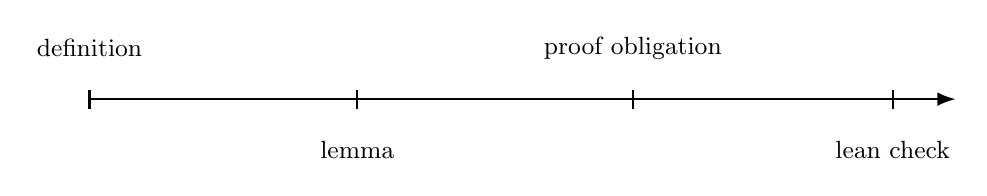
\begin{tikzpicture}[node distance=1.35cm,>=Latex,every node/.style={font=\small}]
\draw[->,thick] (0,0) -- (11,0);
\node[align=center] at (0,0.65) {definition};
\node[align=center] at (3.4,-0.65) {lemma};
\node[align=center] at (6.9,0.65) {proof obligation};
\node[align=center] at (10.2,-0.65) {lean check};
\foreach \x in {0,3.4,6.9,10.2} \draw[thick] (\x,0.12) -- (\x,-0.12);
\end{tikzpicture}
\caption{Theorem Roadmap: historical timeline of proof dependency pressure 47-1-42}
\label{fig:figure-theorem-roadmap-one}
\end{figure}
The point of the diagram is not decoration; it marks which relation is being proposed and which stronger conclusion is still unavailable.\par
A local clarification is useful here\par
A local clarification is useful here\footnote{In Theorem Roadmap, this note clarifies the reader clarification role of the term and keeps the caveat close to the sentence that needs it.}.\par
The note keeps the caveat near the term without derailing the main sentence.\par
The first words can be simple. A continuum is a range along which something may vary while still belonging to the same field of description. A boundary is a condition that separates what the description permits from what it does not permit. An operator is an action, transformation, or constraint that changes a configuration or preserves some part of it. A contradiction, in the sense used here, is not a mere annoyance or verbal tension. It is a conflict inside a described configuration that cannot be removed by changing names while leaving the structure intact.\par
With those words in place, the central hypothesis can be stated carefully. When a system is described by a range of possible variation, by boundaries on admissible states, by operations that transform or preserve structure, and by a conflict the present description cannot absorb, some changes may be understood as transitions between descriptions. In one direction, the system may require a new dimension of description: a new variable, relation, or level at which the relevant pattern becomes intelligible. In the other direction, the system may collapse: it can no longer maintain the relations that made it recognizable as the configuration under discussion.\par
The point of a theorem roadmap is to keep this claim from floating as metaphor. It does not ask the reader to accept the theory in advance. It prepares the question a theorem would have to answer. What exactly is the object? Which boundaries are operative? Which transformations are allowed? What counts as unresolved conflict? What would distinguish expansion into a richer description from ordinary change, and what would distinguish collapse from interruption, damage, or external shock? A theory that cannot answer those questions has not yet earned the word theorem.\par
\section{The Dependency Spine In Theorem Roadmap}
The vocabulary becomes clearer when it is allowed to move. A continuum is not simply a variable with a grander name. It is a field of possible variation that remains legible under a description. Temperature may vary across a body of water. Density may vary with temperature. Velocity may vary from point to point. None of these variations, by itself, requires a new kind of object. They are changes within an existing descriptive frame. \cite{wilson_renormalization,landau_stat_physics}\par
A boundary is not merely a wall. The glass or metal container is a boundary, but so are gravity, viscosity, heat flux, conservation laws, and the equations that say which states can follow from which states. A boundary tells the description what cannot simply be wished away. If warm fluid rises, it does so under gravity. If motion begins, viscosity resists it. If heat enters through the bottom and leaves through the top or sides, that imposed asymmetry matters. The boundary is the discipline of the scene.\par
The local dependency can now be written without changing the claim it supports.\par
\begin{equation}\label{eq:equation-theorem-roadmap-two}
\operatorname{regularityResidual}_{11} = \tau_{\mathrm{repair}}=\inf\{t:C(t)<\theta\}
\end{equation}
The relation names a local dependency, variable dictionary, and proof/evidence role; it is not a claim-status upgrade.\par
The formula is a restraint on the prose. It names the dependency that the surrounding paragraph is allowed to use.\par
The comparison below gives theorem roadmap a set of quantities that can be inspected instead of merely admired.\par
\begin{table}[htbp]
\centering\small
\caption{Theorem Roadmap: observable quantities and counter-pressure 47-2-42}
\label{tab:table-theorem-roadmap-one}
\begin{tabular}{@{}llll@{}}
\toprule
Projection & Domain quantity & Comparator & Limit \\
\midrule
theorem roadmap boundary & 48 units & declared case & fixes what is compared \\
residual pressure & 0.21 & dimensionless & shows unresolved load \\
projection loss & 0. & bounded interval & marks lost structure \\
countercase set & 21 cases & review sample & keeps a falsifier visible \\
\bottomrule
\end{tabular}
\end{table}
The table should be read locally: it narrows the comparison without pretending that the wider theory has been settled by a single surface.\par
An operator is the language of permitted action. Diffusion moves heat down a gradient. Buoyancy converts density difference into upward force. Viscosity damps motion and transfers momentum. A stirring spoon would be another kind of operator, but it would change the example because it would introduce an external driver. Operators matter because they prevent the theory from saying, vaguely, that things change. They specify how a configuration may be transformed.\par
Hierarchy enters when one description depends on another without being exhausted by it. The macroscopic roll of a convecting fluid depends on molecular motion, temperature, density, and momentum transfer, but the roll is not conveniently described by naming every molecule. It has a shape, persistence, and orientation that belong to a higher-level account. The lower-level facts do not vanish. They remain necessary. Yet the pattern that the observer needs to understand has become a macroscopic object of attention.\par
This is the kind of hierarchy OC cares about. It is not a license to treat every loose collection as an emergent whole. A pile of facts is not a hierarchy merely because it is large. A hierarchy requires dependence, constraint, and a relation between descriptions. The lower description must support the higher one, and the higher one must identify something not efficiently captured by the lower description alone. Otherwise, the word adds ceremony without explanation.\par
\section{Lean As A Restraint In Theorem Roadmap}
Return to the heated fluid. At first the bottom layer warms, expands, and becomes lighter than the cooler fluid above it. The situation is strained but still quiet. Heat diffuses upward. Tiny motions are damped. The macroscopic description remains close to rest. A thermometer would register difference; the eye might see almost nothing. The old description is not false. It is simply adequate for the regime it is describing. \cite{wilson_renormalization,landau_stat_physics}\par
As the temperature difference grows, the strain becomes harder for the old description to contain. Warm, lighter fluid below cool, heavier fluid above is an unstable arrangement under gravity. Buoyancy favors upward motion, while viscosity and diffusion resist the formation of organized flow. Below a threshold, resistance and smoothing dominate. Above it, the balance changes. Small disturbances no longer disappear in the same way. They can be amplified into circulation. Rising warm fluid and sinking cool fluid form rolls, cells, or other organized patterns depending on the shape of the container and the imposed conditions.\par
The local dependency can now be written without changing the claim it supports.\par
\begin{equation}\label{eq:equation-theorem-roadmap-one}
\operatorname{complexityVerifier}_{11} = \operatorname{loss}_{\phi}=1-\frac{|E_{\phi}\cap E_{\mathrm{domain}}|}{|E_{\mathrm{domain}}|}
\end{equation}
The relation names a local dependency, variable dictionary, and proof/evidence role; it is not a claim-status upgrade.\par
The formula is a restraint on the prose. It names the dependency that the surrounding paragraph is allowed to use.\par
The local dependency can now be written without changing the claim it supports.\par
\begin{equation}\label{eq:equation-theorem-roadmap-three}
\operatorname{rankGrowthToy}_{11} = I_{\mathrm{axis}}=\frac{\operatorname{Var}(x\mid a)}{\operatorname{Var}(x)}
\end{equation}
The relation names a local dependency, variable dictionary, and proof/evidence role; it is not a claim-status upgrade.\par
The formula is a restraint on the prose. It names the dependency that the surrounding paragraph is allowed to use.\par
A small numerical test keeps the abstraction honest at the scale of a single decision.\par
\paragraph{Numerical example.} For theorem roadmap, take support=0.53, projection loss=0.15, and 4 open obligations. The bounded score is 0.; the example gives the reader a numeric scale without pretending to be empirical proof.\par
The numbers are deliberately small; their value is pedagogical, not evidential, unless the chapter binds them to a dataset elsewhere.\par
The important change is not merely that the fluid moves. Many things move without requiring a new explanatory level. The important change is that motion becomes organized enough to be described as a pattern with its own variables. One may now ask about the size of the rolls, their direction, their stability, and their response to further heating. The relevant description has acquired a macroscopic order parameter or pattern variable. A longer inventory of microscopic positions would be possible in principle, but it would not be the natural way to state what changed.\par
This example also shows why the language of contradiction must be handled with restraint. It would be careless to say that contradiction alone causes convection. The physical account involves thermal gradients, density differences, gravity, viscosity, geometry, and governing equations. OC can learn from the case only by respecting those conditions. The conflict is not a mystical force. It is a structured incompatibility between a maintained arrangement and the operations acting within the boundaries of the system.\par
In that restrained sense, the example is useful. The fluid initially admits a description in which macroscopic stillness is adequate. The growing temperature difference introduces a condition under which that description ceases to capture the dominant organization. The system does not simply add more of the same. It crosses into a regime where a new macroscopic variable becomes necessary. If the container cracks, or the heat source fails, or the fluid boils violently under conditions outside the intended model, the example changes. Those cases might be collapse, external interruption, or a different phenomenon altogether. The classification has to follow the system, not the appetite of the theory.\par
\section{A Proof Boundary In Theorem Roadmap}
This way of thinking has neighbors in established science, and it should be read in that modest company. Kenneth Wilson's work on renormalization changed how physicists understood scale. It showed that a system can have stable descriptions at different levels, and that the variables useful at one scale may not be the variables one would choose at another. The microscopic details do not become unreal, but they may cease to be the most explanatory objects for the question at hand. \cite{wilson_renormalization,landau_stat_physics}\par
Landau's statistical physics gave another lesson: transitions often become intelligible when one identifies an order parameter. A material may change phase, and the change is not captured well by saying only that all its particles moved a little. Something about the collective state has altered. The order parameter gives the theory a handle on that alteration. It names the feature through which the transition can be tracked.\par
The case that follows turns the proposal into a sequence of criticizable moves.\par
\paragraph{Worked case.} In the worked case for theorem roadmap, the claim is reduced to a boundary, an observable, a dependency, a numerical cue, and a falsifier. The case is useful only because each move can be criticized separately.\par
The case helps because each step can fail separately, which is exactly what a useful example should permit.\par
Ilya Prigogine's work on dissipative structures emphasized that order can be maintained far from equilibrium. In such systems, pattern is not always the sign of rest or simple stability. It may depend on flows of energy and matter through the system. Order may be something the system continually does. Hermann Haken's synergetics likewise studied how macroscopic order can arise from the interaction of many components, with a few collective variables guiding the behavior of many parts.\par
OC does not claim to absorb these traditions or improve them by renaming them. The lesson it takes is narrower. A serious account of emergence must say which variables are being used, which constraints are active, which transformations are allowed, and what counts as a successful description. Without those commitments, the language of emergence becomes too easy. It can be attached to any surprising pattern after the fact.\par
The theorem roadmap therefore belongs less to the rhetoric of discovery than to the discipline of description. It asks how a claim about transition can be made inspectable. If a system is said to expand into a new descriptive dimension, the new dimension must be named. If a system is said to collapse, the lost structure must be specified. If a contradiction is said to drive the change, the incompatible requirements must be shown inside the model rather than announced from outside it.\par
\section{What Remains Conditional In Theorem Roadmap}
A theorem begins when the prose stops leaning on atmosphere and starts naming its commitments. The object must be specified. It may be a graph, a dynamical system, an algebraic structure, a typed configuration, a state space, or some other formal object. The admissible states must be distinguished from inadmissible ones. The transformations must be named. The relation called contradiction must be defined strongly enough that a reader can tell when it is present and when it is not. \cite{wilson_renormalization,landau_stat_physics}\par
From there, the possible outcomes have to be stated without drama. Dimensional expansion means that the existing description lacks a coordinate, relation, type, or level required to preserve intelligibility under the stated conditions. Collapse means that the existing configuration loses the relations required for its identity as that configuration. Neither term should be used as a flourish. Expansion is not ordinary improvement. Collapse is not every unpleasant change. Both require criteria.\par
The strongest possible result would show that certain patterns of unresolved conflict force one of these outcomes. Such a result would need assumptions precise enough to bear the weight. It would need to exclude cases where the apparent conflict is only a bad description, cases where the transition is caused by an external shock, and cases where the system can absorb the tension through an already available adjustment. The more ambitious the theorem, the narrower and clearer its assumptions must become.\par
There are several degrees of maturity in such work. A conceptual claim explains how the theory is meant to operate. It may guide intuition and organize examples, but it does not by itself prove that the proposed structure must behave as described. A mathematical claim states objects, assumptions, and conclusions in a form that can be inspected and argued over. A mechanically checked claim is expressed in a proof assistant such as Lean, where each formal inference is verified by software against accepted rules and definitions.\par
These distinctions are not administrative decoration. They protect the reader. They also protect the theory from pretending to have arrived earlier than it has. A sentence in prose may be suggestive and true to the intended idea, while still falling short of a mathematical statement. A mathematical statement may be rigorous on paper, while still not having been encoded for mechanical checking. A Lean theorem may verify exactly what it states, while saying nothing about the surrounding analogies unless those analogies have also been formalized. Each form of claim has its own strength and its own boundary.\par
\section{The First Formal Move In Theorem Roadmap}
Lean is a proof assistant: a system for writing definitions and proofs so that a computer can check whether each inference follows from accepted rules and previously defined material. Its presence in this monograph is therefore not ornamental. It marks a place where the argument has been forced into a formal language. It also marks the edge of that formalization. The checked statement is not automatically as wide as the prose that surrounds it. \cite{wilson_renormalization,landau_stat_physics}\par
That edge matters because the central words of OC are large words. Continuum, boundary, operator, hierarchy, contradiction, emergence, expansion, and collapse all carry histories from mathematics, physics, philosophy, and ordinary speech. In ordinary prose, such words can move too quickly. They can seem to explain because they sound powerful. Formalization slows them down. It asks what the objects are, what relations are allowed, what functions or transformations exist, and what conclusion follows.\par
A formal statement also exposes disappointment. It may reveal that a cherished phrase has no stable definition. It may show that a supposed theorem needs an assumption so strong that the result becomes less interesting. It may discover that two concepts kept apart in prose collapse into one object when formalized, or that one concept in prose actually contains several different formal notions. This is not a failure of seriousness. It is what seriousness often looks like.\par
The formal boundary should therefore be read as a line of honesty. On one side are definitions and checked inferences. On the other side are interpretation, motivation, examples, and scientific ambition. The two sides may support each other, but they are not the same. A proof assistant can verify a theorem about a defined structure. It cannot, by that fact alone, prove that a biological organism, a market, a mind, or a research institution instantiates that structure. Domain application has to be earned separately.\par
This is especially important for a theory that wants to speak across domains. Cross-domain language is useful only when it remains answerable to the observables of each domain. A pattern in a fluid, a developmental shift in an organism, a change in a scientific field, and a transition in a computational system may share a formal shape at some level of abstraction. But the evidence that each case actually fits the shape must come from the domain itself. Otherwise, abstraction becomes a way of ignoring the world rather than understanding it.\par
\section{The Dependency Spine In Theorem Roadmap roadmapS}
A theorem worth pursuing must invite the cases that might defeat it. One possible counterexample would be a system that appears to contain unresolved contradiction but neither expands into a new descriptive dimension nor collapses. Another would be a system in which a new descriptive dimension appears without any relevant internal conflict. A third would be a collapse caused by an external shock rather than by internal incompatibility. A fourth would be a case where the alleged contradiction vanishes once the variables are described more carefully. \cite{wilson_renormalization,landau_stat_physics}\par
These cases do not automatically refute OC, but they force it to become narrower and better. Perhaps the original claim applies only to a specific class of structured descriptions. Perhaps the contradiction must be defined as a failure of simultaneous satisfiability under named operators. Perhaps expansion requires not merely a new vocabulary but a demonstrable preservation of the old configuration through a richer structure. Perhaps collapse requires loss of identity conditions rather than mere degradation. Counterexamples are not interruptions to the work. They are part of how the work becomes scientific.\par
The fluid example again shows the need for discipline. If convection appears, the theory must not declare victory because a pattern emerged. It must ask what was measured, what equations govern the system, what thresholds are known, what boundaries were imposed, and whether the old description was genuinely inadequate for the question being asked. If a new macroscopic variable is introduced, the theory must say why that variable is not merely convenient but required for the explanation under consideration.\par
The same caution applies elsewhere. In biology, a developmental transition may involve new levels of organization, but the relevant observables are not the same as those in fluid mechanics. In social systems, conflict may produce institutional change or breakdown, but social categories are not particles, and their boundaries are partly maintained by interpretation and practice. In cognition, a problem may require a new representation, but one must distinguish representational shift from simple learning or memory retrieval. In computation, a system may move to a richer type or state representation, but only the specified machine, language, or process can say what that means.\par
The discipline is simple to state and hard to satisfy: do not project the theory faster than the evidence travels. An example may illustrate a pattern. It may test a claim. It may motivate a definition. It may resemble the structure without instantiating it. These are different relations. Keeping them apart is not pedantry. It is the difference between a theory that can learn from failure and a vocabulary that only collects confirmations.\par
\section{Lean As A Restraint In Theorem Roadmap roadmapS}
A reader can therefore approach the theorem roadmap as a training of attention. When a claim appears, ask first what kind of claim it is. If it is conceptual, it should clarify the intended movement of thought. If it is mathematical, it should expose its objects and assumptions. If it is mechanically checked, it should be read with care for the exact statement that has been checked. The higher status does not automatically spread to every nearby sentence. \cite{wilson_renormalization,landau_stat_physics}\par
Then ask what the description is doing. Is a continuum being named, or only a variable? Is a boundary being specified, or only an obstacle? Is an operator defined, or only an event narrated? Is a hierarchy shown through dependence between descriptions, or is it merely a stack of parts? Is a contradiction present inside the structure, or is the word being used for inconvenience, opposition, or surprise? Is expansion the introduction of a necessary descriptive dimension, or merely the addition of more detail? Is collapse the loss of identity-preserving relations, or simply damage?\par
These questions make later claims easier to accept when they are strong and easier to reject when they overreach. That is the proper service of the chapter. It does not ask the reader to believe that every complex system obeys one grand rule. It asks the reader to watch how a description bears strain, how its boundaries restrict change, how its operations transform what is possible, and how a conflict may force either richer articulation or loss of form.\par
A theorem, in this setting, is not a ceremonial endpoint. It is a compact way of making responsibility visible. It says: under these conditions, for this kind of object, with these transformations and these boundaries, this conclusion follows. Everything outside that sentence may still matter, but it has not been smuggled into the proof. The dignity of the theorem is its refusal to say more than it has earned.\par
That refusal is also what allows the larger project to breathe. OC can speak about emergence, contradiction, expansion, and collapse only if it is willing to slow those words down until they become answerable. The heated fluid helps because it shows a description becoming insufficient in a concrete case: warmth accumulating below, buoyancy pressing upward, resistance delaying motion, and then a visible order appearing where stillness had been enough. The formal vocabulary helps because it asks which parts of that story can be generalized. The boundary of proof helps because it prevents the example from becoming a universal law by enthusiasm alone.\par
The arrival point is a disciplined posture. A reader who has followed this chapter can not come away with a slogan, but with a set of habits: locate the object, name the allowed variation, identify the boundary, specify the operation, test the alleged contradiction, and distinguish expansion from collapse. These habits do not make the theory true. They make its truth or failure more visible. That is the work a theorem roadmap can honestly do.\par
\chapter{Proof Obligation Graph}
\section{From Claim To Obligation In Proof Obligation Graph}
A Proof Obligation Graph is a map of what has to be established before a claim can be used by later thought. It begins from a simple uneasiness: ambitious language often travels faster than its warrants. A sentence may sound exact because it contains words such as operator, boundary, continuum, hierarchy, or dimension, yet those words do not carry the same weight in every setting. The graph slows the sentence down. It asks what each part depends on, what kind of support each dependency has, and where a reader can pause before granting the next step. \cite{landau_stat_physics,prigogine_dissipative}\par
This is not a device for making thought timid. It is a way of preserving the difference between a fertile hypothesis and an earned conclusion. A good theory needs both. It needs concepts that can reach beyond present demonstrations, and it needs a memory of what has actually been shown. The Proof Obligation Graph supplies that memory. It can record a definition, an example, a mathematical route, an external scientific result, a modeling assumption, an analogy, a missing observation, or an open problem without pretending that these are all the same kind of support.\par
The next diagram slows the argument down just enough to show how proof obligation graph is being organized.\par
\begin{figure}[htbp]
\centering
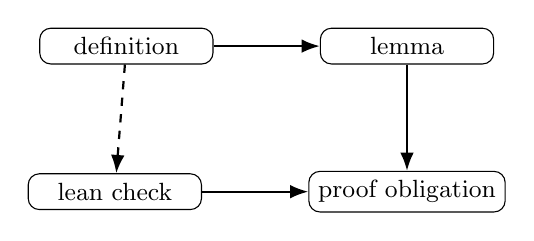
\begin{tikzpicture}[node distance=1.35cm,>=Latex,every node/.style={font=\small}]
\node[draw,rounded corners,align=center,minimum width=2.2cm] (a) {definition};
\node[draw,rounded corners,align=center,minimum width=2.2cm,right=of a] (b) {lemma};
\node[draw,rounded corners,align=center,minimum width=2.2cm,below=of b] (c) {proof obligation};
\node[draw,rounded corners,align=center,minimum width=2.2cm,left=of c] (d) {lean check};
\draw[->,thick] (a) -- (b);
\draw[->,thick] (b) -- (c);
\draw[->,thick] (d) -- (c);
\draw[->,thick,dashed] (a) -- (d);
\end{tikzpicture}
\caption{Proof Obligation Graph: dependency dag of proof dependency pressure 48-1-43}
\label{fig:figure-proof-obligation-graph-one}
\end{figure}
The point of the diagram is not decoration; it marks which relation is being proposed and which stronger conclusion is still unavailable.\par
A local clarification is useful here\par
A local clarification is useful here\footnote{In Proof Obligation Graph, this note clarifies the reader clarification role of the term and keeps the caveat close to the sentence that needs it.}.\par
The note keeps the caveat near the term without derailing the main sentence.\par
Consider a layer of fluid heated from below. At low heating, heat may move mainly by conduction. As heating increases, the uniform conductive state may lose stability and organized convection rolls may appear. The ordinary words in that sentence already carry technical shadows. A boundary condition fixes something about the edge of the system, such as temperatures at the top and bottom plates. A control parameter is a quantity whose variation changes the regime, such as a temperature gradient or a nondimensional number used in the model. An instability is not merely excitement or turbulence in ordinary speech, but a failure of a state to persist under specified perturbations. An order parameter, in traditions such as synergetics, is a macroscopic variable that can summarize and coordinate the behavior of many smaller components.\par
These terms are introduced here first as scientific orientation, not as automatic possessions of OC. The book's own use of dimension also needs care. In stricter mathematics, a dimension may be a coordinate degree in a specified space. In physics, it may refer to measurable degrees of freedom or units of analysis inside a model. In OC, unless a stricter sense is explicitly supplied, dimension means an operational axis of description: a way of distinguishing states, constraints, or transformations that the previous description could not adequately carry. That sense can be useful, but it does not become mathematical merely by borrowing the word.\par
With that distinction in place, the central hypothesis can be stated without inflation: an unresolved contradiction may give rise to a new dimension of description or may collapse the configuration that cannot resolve it. The sentence is intentionally strong. It proposes a pattern by which systems may move beyond an exhausted descriptive arrangement. But the sentence also opens obligations. The contradiction has to be named. The old description has to fail in a determinate way. The proposed new dimension has to do explanatory work. Collapse has to remain a real alternative rather than a discarded inconvenience.\par
An obligation is the smallest named burden that a later claim depends on. If the claim says that a contradiction opens a new dimension, the graph does not let the phrase pass whole. It asks what counts as contradiction, what arrangement contains it, what kind of failure it produces, what the new dimension changes, and what would count against the claim. The point is not to drain the idea of force. The point is to make its force reusable. A claim that carries its obligations openly can be compared, criticized, strengthened, or transported into another domain without becoming vapor.\par
The heated fluid example shows why this matters. Classical statistical physics, represented in one lineage by Landau's care with macroscopic order and transitions, teaches that order is not granted by description alone. One needs variables, regimes, assumptions, and criteria. A pattern of convection rolls is not just a pretty picture imposed on motion. It becomes a scientific object through a model that identifies the system, the boundary conditions, the relevant parameters, the instability threshold, and the observable pattern that distinguishes one regime from another. OC can learn from this discipline of articulation without claiming that every OC transition is a physical phase transition.\par
The graph protects later reasoning from borrowing more certainty than earlier reasoning has earned. It lets the reader see whether a statement is a proposed concept, a worked example, a theorem, a modeling analogy, or a research program. This separation is constructive. It makes comparison cleaner, helps claims survive outside the paragraph in which they first sound plausible, and turns large theoretical ambition into a sequence of visible burdens.\par
\section{The Dependency Spine In Proof Obligation Graph}
Every serious claim has a history inside it. Some parts come from definitions. Some come from examples. Some come from established mathematics or science. Some come from translation into a new domain. The dependency chain is the ordered relation among these parts. It tells the reader which obligations have to be settled first and which later claims lose force if an earlier one fails. \cite{landau_stat_physics,prigogine_dissipative}\par
In the fluid case, the chain begins before the word emergence appears. First there is a system: a fluid layer, not an undefined mass of motion. Then there are boundaries: plates, temperatures, constraints on the domain. Then there is energy flow: heating from below and cooling above. Then there is a control parameter whose increase can move the system toward a new regime. Then there is a criterion for instability, which in the familiar convection story can be associated with threshold reasoning such as the onset of Rayleigh-Benard convection. Only after those pieces are in view does it become meaningful to ask whether organized rolls count as a new macroscopic order.\par
The local dependency can now be written without changing the claim it supports.\par
\begin{equation}\label{eq:equation-proof-obligation-graph-two}
\operatorname{institutionalLatency}_{11} = \rho_{\mathrm{replay}}=\frac{N_{\mathrm{matched}}}{N_{\mathrm{declared}}}
\end{equation}
The relation names a local dependency, variable dictionary, and proof/evidence role; it is not a claim-status upgrade.\par
The formula is a restraint on the prose. It names the dependency that the surrounding paragraph is allowed to use.\par
The comparison below gives proof obligation graph a set of quantities that can be inspected instead of merely admired.\par
\begin{table}[htbp]
\centering\small
\caption{Proof Obligation Graph: observable quantities and counter-pressure 48-2-43}
\label{tab:table-proof-obligation-graph-one}
\begin{tabular}{@{}llll@{}}
\toprule
Proof object & Dependency & Lean surface & Closure state \\
\midrule
proof obligation graph boundary & 51 units & declared case & fixes what is compared \\
residual pressure & 0.28 & dimensionless & shows unresolved load \\
projection loss & 0.13 & bounded interval & marks lost structure \\
countercase set & 22 cases & review sample & keeps a falsifier visible \\
\bottomrule
\end{tabular}
\end{table}
The table should be read locally: it narrows the comparison without pretending that the wider theory has been settled by a single surface.\par
Prigogine's work on dissipative structures is relevant here because it treats ordered structures maintained far from equilibrium. Haken's synergetics is relevant because it studies how macroscopic order parameters can organize the behavior of many microscopic components. These references orient the reader toward scientific treatments of order, instability, and collective pattern. They do not prove OC's general vocabulary. They show the level of care required when a theory speaks of order emerging through constraint, flow, and transformation.\par
The dependency chain also identifies the kind of movement being made. A claim about the meaning of OC vocabulary may depend only on internal definitions. A claim about a physical system may depend on a model and external scientific results. A claim about a social, cognitive, or biological system requires a disciplined projection: it has to say what counts as a state, a boundary, an operator, a contradiction, a collapse, and an observable change in that domain. Without this projection, the argument is only resemblance dressed in stronger clothing.\par
Many large theories lose precision at exactly this point. They begin with a physical example, then notice a similarity in another domain, then let similarity harden into explanation. The movement is understandable. Good analogies are often where inquiry begins. But analogy and proof do different work. A weak dependency may motivate, illustrate, or suggest a direction. A strong dependency is one without which the later claim fails. The graph helps a reader see which kind of edge is being crossed.\par
Strong and weak dependencies are not moral rankings. A weak analogy can be intellectually valuable. It may reveal a pattern worth testing or a vocabulary worth refining. Its weakness only means that it cannot bear the full weight of the later conclusion. A strong dependency, by contrast, is load-bearing. If the definition of contradiction fails, then any claim built on that definition weakens with it. If the external theorem does not apply to the domain being discussed, the imported support disappears.\par
In OC language, this distinction clarifies the work done by contradiction. A contradiction is not any tension, puzzle, inconvenience, or complexity. It is an unresolved incompatibility within a given descriptive arrangement. The dependency chain asks where that arrangement is specified, why the incompatibility cannot be removed within it, and what happens next. Sometimes the next step may be the introduction of a new descriptive axis. Sometimes it may be collapse, understood as a loss of configuration, admissibility, or operational coherence. Sometimes the honest answer is that the case has not yet been shown.\par
The benefit is not only restraint. A visible dependency chain makes the theory easier to extend. Later chapters can reuse a definition without restating its entire defense. A reader can compare two examples and see whether they share a structural role or only a surface resemblance. A research program can focus on the missing link rather than arguing repeatedly over the whole system. The chain turns broad ambition into a set of places where further work can actually enter.\par
\section{Lean As A Restraint In Proof Obligation Graph}
The idea becomes clearer when the graph is drawn in miniature. Take the claim: C0, 'In the heated fluid case, the appearance of convection rolls illustrates how a prior description can become insufficient and a new macroscopic descriptive variable can become necessary.' The wording matters. C0 says illustrates. It does not say proves the central OC hypothesis in all domains. The claim is therefore allowed to be useful while remaining modest. \cite{landau_stat_physics,prigogine_dissipative}\par
The graph begins with definition nodes. D1 is 'system specified': a fluid layer heated from below and cooled above. D2 is 'boundary condition specified': the top and bottom constraints are fixed in the model or example. D3 is 'control parameter identified': the relevant measure of heating is named. D4 is 'instability criterion named': the route by which the conductive state loses stability is not left as a metaphor. D5 is 'OC dimension qualified': dimension is being used as an operational axis of description unless a stricter mathematical sense is supplied.\par
The local dependency can now be written without changing the claim it supports.\par
\begin{equation}\label{eq:equation-proof-obligation-graph-one}
\operatorname{socialCoordination}_{11} = G=(V_{\mathrm{claim}}\cup V_{\mathrm{evidence}},E_{\mathrm{support}}\cup E_{\mathrm{challenge}})
\end{equation}
The relation names a local dependency, variable dictionary, and proof/evidence role; it is not a claim-status upgrade.\par
The formula is a restraint on the prose. It names the dependency that the surrounding paragraph is allowed to use.\par
The local dependency can now be written without changing the claim it supports.\par
\begin{equation}\label{eq:equation-proof-obligation-graph-three}
\operatorname{biologicalRobustness}_{11} = \epsilon_{\mathrm{domain}}=\max_i |y_i-\hat y_i|
\end{equation}
The relation names a local dependency, variable dictionary, and proof/evidence role; it is not a claim-status upgrade.\par
The formula is a restraint on the prose. It names the dependency that the surrounding paragraph is allowed to use.\par
A small numerical test keeps the abstraction honest at the scale of a single decision.\par
\paragraph{Numerical example.} For proof obligation graph, take support=0.56, projection loss=0., and 5 open obligations. The bounded score is 0.; the example gives the reader a numeric scale without pretending to be empirical proof.\par
The numbers are deliberately small; their value is pedagogical, not evidential, unless the chapter binds them to a dataset elsewhere.\par
Next come scientific and modeling nodes. E1 is 'external theorem or tradition cited': threshold reasoning in convection and the broader physics of instability and macroscopic order. Its status is external scientific support for the physical case, not internal proof of OC. M1 is 'model assumption exposed': the example depends on idealizations about the fluid, geometry, boundary conditions, and parameter range. O1 is 'observation or phenomenon identified': organized convection rolls appear as a macroscopic pattern under the relevant conditions. I1 is 'interpretive bridge': the old low-level thermal description is said to be insufficient for the patterned macroscopic state, and a new descriptive variable becomes useful.\par
The edges between these nodes carry different force. D1, D2, D3, and D4 have strong dependency edges into the physical part of C0, because without a specified system, boundary, parameter, and instability criterion, the convection story becomes loose imagery. E1 has a strong edge into the claim that the physical example belongs to a serious scientific tradition, but only a weak edge into the OC generalization. M1 has a strong edge into the scope of the example, because the model assumptions determine where the physical reasoning applies. O1 has a strong edge into the assertion that there is a pattern to discuss. I1 has a weak-to-moderate edge into the OC vocabulary, because it translates a physical transition into a descriptive lesson.\par
The graph can now mark statuses. D1 through D5 may be 'defined for this discussion' if their meanings are fixed locally. E1 may be 'externally established in the relevant scientific literature' only for the physical tradition it actually belongs to. M1 may be 'assumed for the example.' O1 may be 'observed or standard phenomenon,' depending on whether the text is referring to experiment, simulation, or canonical presentation. I1 is 'conceptual interpretation.' C0 is therefore not stronger than its path permits: it is a disciplined illustration, not a theorem of OC.\par
Now add a tempting claim: C1, 'Because convection rolls arise in the heated fluid, every unresolved contradiction in any domain generates a new dimension of organization.' The graph blocks it. The edge from E1 to C1 is too weak; a physical result about a modeled fluid layer cannot carry an unrestricted cross-domain law. The edge from I1 to C1 is also too weak; an interpretive bridge does not become a universal theorem. A new node would be required, P1, 'domain-general projection rule established,' and another, P2, 'conditions for contradiction, emergence, and collapse specified across domains.' In the present graph, P1 and P2 are absent.\par
The blocked node is therefore B1, 'OC-generalization from convection to all domains.' Its status is blocked, not because the example is useless, but because the intended conclusion asks for a stronger route than the graph contains. The block is precise. It does not say that OC cannot develop a general claim. It says that the general claim would need additional definitions, projection rules, comparisons, perhaps formal models, and domain-specific evidence. The physical example can still motivate the search. It cannot finish it.\par
This miniature graph is the chapter's central discipline in action. It shows how a claim can be allowed to breathe without being allowed to sprawl. The fluid example gives OC a scene of use: boundaries, parameters, instability, order, and new description. The graph then preserves the distinctions that make the scene intellectually honest. Scientific support remains scientific support. Analogy remains analogy. Conceptual translation remains translation. A blocked generalization becomes a research task rather than a smuggled conclusion.\par
\section{A Proof Boundary In Proof Obligation Graph}
A proof route is the path through the graph by which a mathematical or formal claim could be established. It begins with definitions, moves through assumptions and intermediate results, and ends with a conclusion whose strength is limited by the weakest required step. The route may be complete, partial, informal, conjectural, or absent. Those differences matter because OC uses language that can sound mathematical before it has earned mathematical force. \cite{landau_stat_physics,prigogine_dissipative}\par
Terms such as continuum, operator, projection, hierarchy, and collapse can be defined carefully, but definition alone does not produce a theorem. A theorem needs a setting, admissible objects, assumptions, and a valid derivation. If continuum is a structured range of possible states or descriptions, the proof route has to say what structure is present. If an operator changes a continuum, the route has to say what kind of object the operator is, what counts as change, and whether the resulting object remains within the same universe of discourse. If collapse is a loss of configuration or admissibility, the route has to specify the conditions under which that loss occurs.\par
The case that follows turns the proposal into a sequence of criticizable moves.\par
\paragraph{Worked case.} In the worked case for proof obligation graph, the claim is reduced to a boundary, an observable, a dependency, a numerical cue, and a falsifier. The case is useful only because each move can be criticized separately.\par
The case helps because each step can fail separately, which is exactly what a useful example should permit.\par
The convection example contains a contrast between two routes. One route belongs to mathematical physics. It may begin with equations for a fluid layer under a temperature gradient, impose boundary conditions, analyze stability, and derive a threshold at which the conductive state becomes unstable. In the familiar Rayleigh-Benard setting, the reasoning can be tied to a critical value of a control parameter, after which convection becomes the relevant patterned regime. That is a route with technical content. It does not rest on the word emergence; it earns its conclusion through model, parameter, and derivation.\par
A second route is conceptual. It asks what OC can learn from the form of the case. The low-heating description is adequate for one regime. A stronger heating condition brings forward a macroscopic pattern that calls for a different descriptive vocabulary. The new vocabulary is not ornamental; it captures something the earlier description did not foreground. This route can illuminate the OC hypothesis by showing how a new descriptive axis may become useful when a prior arrangement reaches its limit. But it remains conceptual unless the OC terms are formalized and the derivation is supplied.\par
The two routes can coexist without confusion if the graph keeps them separate. The physics route may carry mathematical or empirical authority within its domain. The OC route may carry interpretive and architectural value. A reader can then ask the right question of each. For the physics route: are the equations, assumptions, and threshold analysis valid for the system described? For the OC route: has the text specified what counts as contradiction, new dimension, emergence, and collapse in this setting?\par
This separation gives bold ideas a better future. Without it, the prose is tempted to lean on borrowed authority. With it, the theory can say: here is a physical case with its own scientific route; here is the conceptual pattern OC sees in it; here is what remains to be done before the conceptual pattern becomes a theorem or a domain-general model. That honesty does not weaken the claim. It keeps the claim from being used in ways that would later make it brittle.\par
An objection naturally arises: does this make the theory too cautious to be interesting? It should have the opposite effect. A theory becomes more usable when its claims can be sorted by present status. Readers can adopt a definition, test an example, challenge a dependency, build a model, or attempt a proof without first deciding whether the whole architecture stands or falls. The graph lets inquiry enter at many points.\par
A proof route also improves disagreement. If two readers dispute a later OC claim, the graph can show whether they disagree about a definition, an assumption, an analogy, an external result, or an inference. This is better than a general quarrel over tone or plausibility. The argument becomes local enough to repair. A missing lemma can be supplied. A projection can be narrowed. A claim can be demoted from theorem to hypothesis. A better example can replace a weaker one.\par
\section{What Remains Conditional In Proof Obligation Graph}
Some claims can live responsibly in ordinary prose. Others ask for a stricter form. A formalization check asks whether the relevant obligations have been expressed in a way that a rigorous formal system could inspect. Ordinary mathematical writing often lets a skilled reader supply context. A formal system is less forgiving. It needs exact definitions, exact assumptions, exact inference rules, and clear statement boundaries. \cite{landau_stat_physics,prigogine_dissipative}\par
This matters because formal-looking prose can hide ambiguity. Suppose the text says that an operator transforms a continuum across a boundary. The sentence may be intelligible at a high level, but the formalization check asks what kind of object the continuum is, what kind of object the operator is, how the boundary is represented, what transformation preserves, and what transformation destroys. It asks whether two regimes are distinct by definition, by measurement, by topology, by dynamics, or by interpretive convention.\par
The check does not require every sentence in the book to become a machine-checkable proof. That would misunderstand the role of a conceptual monograph. It requires formalizable claims to expose enough structure that formalization is possible in principle. Where that structure is not present, the claim can still be conceptual, heuristic, comparative, or programmatic. Those statuses are legitimate when named accurately. They become dangerous only when they are allowed to masquerade as proof.\par
The heated fluid again gives the distinction a concrete form. The sentence 'organized motion appears after sufficient heating' is clear enough for ordinary exposition. A formal claim would require a model, variables, parameter ranges, stability criteria, and a statement of what follows from them. Nicolis and Prigogine's work on self-organization provides important scientific context for the study of order and instability, but citation cannot replace construction inside OC. If OC wants a formal claim, it has to state its own objects and rules.\par
The word dimension is a useful test. In one paragraph it may mean a mathematical coordinate, in another a physical degree of freedom, in another a descriptive axis that lets a system be interpreted differently. The OC sense is the last of these unless otherwise specified: an operational axis of description. The formalization check asks whether a later argument depends on that looser operational sense or on a stricter mathematical one. If the argument changes sense midstream, the graph catches the equivocation.\par
The same check applies to boundary and collapse. A boundary in a differential equation is not the same thing as a social norm, a cognitive limit, or a classification threshold. A collapse in a physical model is not automatically the same as institutional breakdown or conceptual failure. OC may compare these cases by structural role, but the comparison has to state what is preserved. Is it the idea of admissible states? The loss of a configuration? The failure of a rule to generate a stable next step? Formalization begins when such questions receive exact answers.\par
The payoff is constructive. A formalization check tells the reader which parts of OC are ready for strict mathematical inspection and which parts remain conceptual architecture. It helps a later researcher decide where to build. One person may sharpen definitions. Another may produce a model. Another may test a domain projection. Another may find a counterexample. The graph does not merely restrain claims; it organizes work.\par
It also protects ordinary prose. When formal force is not being claimed, the prose can remain readable without smuggling in false precision. A chapter may say that a pattern suggests a new descriptive dimension, provided it does not imply that a theorem has been proved. The graph gives language room to think while keeping a record of what would be needed for stricter claims.\par
\section{From Claim To Obligation In Proof Obligation Graph obligati}
A blocked case is a point where the next claim cannot inherit the intended status. The block may come from a missing definition, an unproved lemma, an unsupported empirical claim, a failed projection into a domain, or an ambiguity that allows incompatible readings. The value of the block is precision. Instead of saying vaguely that more work is needed, it identifies the exact place where the route stops. \cite{landau_stat_physics,prigogine_dissipative}\par
Suppose OC says that an unresolved contradiction leads either to emergence or collapse. Several blocks may appear. One appears if contradiction has not been distinguished from ordinary complexity or tension. Another appears if emergence is named without specifying the new descriptive dimension. Another appears if collapse is treated only as dramatic language rather than as a defined loss of configuration, admissibility, or operational coherence. Each block asks for a different repair.\par
External scientific references can also create blocked cases. Landau, Prigogine, Haken, and Nicolis and Prigogine can orient discussion of order, fluctuation, instability, and macroscopic pattern. They cannot be used as a general warrant for OC claims across all domains. A graph that marks their role as background, analogy, evidence, or imported theorem prevents a familiar error: treating a respected scientific name as if it had already done the work of translation.\par
This is especially important when a concept travels. A control parameter in a physical model is not a loose cultural pressure. A phase transition is not every dramatic change. A boundary condition in a differential equation is not automatically an institutional norm. A macroscopic order parameter in synergetics is not simply any prominent social variable. Translation may still be possible, but it has to say what relation is being preserved and what evidential standard changes along the way.\par
Blocked cases protect the theory from premature unity. OC is built to compare physical, biological, cognitive, and social systems, but comparison is not identity. Two domains may share a structural role while differing sharply in observables, measurement practices, and standards of evidence. That position is stronger than the claim that all domains secretly instantiate the same physical model. It allows cross-domain thought without erasing the domains being compared.\par
The worked graph for convection already contains one such block. The physical case supports a disciplined illustration of regime change and macroscopic description. It does not support the unrestricted claim that every unresolved contradiction in every domain produces a new dimension. To cross that distance, OC would need a domain-general projection rule, a specification of contradiction across domains, and criteria for emergence and collapse that do not merely repeat the desired conclusion. Until then, the generalization remains blocked.\par
A blocked case can become productive in several ways. It may narrow a claim: instead of all domains, only modeled systems with specified states and transitions. It may demote a claim: from theorem to hypothesis, from hypothesis to analogy, from analogy to image. It may open a research task: define collapse, build a simulation, collect domain evidence, compare rival explanations. The block is not an embarrassment. It is the visible edge of the current theory.\par
A mature theoretical language needs this edge. Without it, every successful example becomes a license for expansion. With it, examples can be strong where they are strong and limited where they are limited. The reader is not asked to accept a total system on trust. The reader is shown where the system has definitions, where it has routes, where it has analogies, and where it still owes work.\par
\section{The Dependency Spine In Proof Obligation Graph obligati}
The Proof Obligation Graph gives OC a way to make ambitious sentences publicly readable. It teaches the reader to ask not whether the vocabulary sounds rigorous, but what the vocabulary has been made to carry. A sentence can be beautiful, suggestive, and useful without yet being a theorem. It can also be precise in one domain and merely suggestive in another. The graph keeps these possibilities apart. \cite{landau_stat_physics,prigogine_dissipative}\par
A later claim can carry scientific weight only when its obligations are visible. The reader needs to know which terms have been defined, which dependencies have been established, which proof route could support the claim, whether formal inspection is possible, and where the route is blocked. Without that map, the same sentence may appear as hypothesis, model, metaphor, evidence, or conclusion depending on the generosity of the reader. With the map, disagreement becomes more exact.\par
The central OC hypothesis remains a proposed organizing idea: an unresolved contradiction may give rise to a new dimension of description or may collapse the configuration that cannot resolve it. The graph does not make that hypothesis true. It states what would have to be defined, shown, modeled, or tested before later uses of the hypothesis can bear more weight. This is the difference between having an idea and giving an idea a disciplined future.\par
The graph also supports the book's cross-domain ambition. OC may compare physical, biological, cognitive, and social systems through continua, boundaries, operators, hierarchy, contradiction, emergence, collapse, and projection. But each movement across domains carries its own obligations. A claim supported in one domain may be only suggestive in another. A strong analogy may open inquiry without closing it. A formal result may travel only after its assumptions travel with it.\par
The scientific traditions invoked in this chapter show the standard of care. Landau's treatment of macroscopic order, Prigogine's dissipative structures, Haken's synergetics, and Nicolis and Prigogine's work on self-organization all handle order, instability, and pattern through technical distinctions. OC can stand near such work only by maintaining its own distinctions with comparable seriousness. The point is not imitation. The point is responsibility in the handling of claims.\par
Once the graph is understood, later vocabulary can be read as a set of commitments rather than as ornament. Later mathematical claims can be followed along their routes. Later examples can be checked against their projections. Later limitations can be treated as the exact places where the present theory has not yet earned the next step. The result is not a smaller theory. It is a theory whose growth can be seen, criticized, and continued.\par
\chapter{Lean Formalization Route}
\section{The First Formal Move In Lean Formalization Route}
Lean is an interactive theorem prover. It checks whether a conclusion follows from stated definitions and assumptions. That is a precise and valuable task, but it is not the same as measuring a system, confirming a scientific model, or discovering a new fact about the world. A theorem in Lean says, in effect: if these objects are defined in this way, and if these hypotheses hold, then this result follows. The force of the result is conditional. \cite{prigogine_dissipative,haken_synergetics}\par
For OC, that distinction matters from the first page of any formal discussion. Several words that sound familiar in ordinary language become technical once they are used in the theory. A continuum is a dimension or range along which a system can vary or be described. A boundary is a rule, threshold, relation, or distinction that determines what counts as inside a configuration, outside it, or observable from a given standpoint. An operator is an action or transformation that changes a state, a description, or a relation. A contradiction is not merely a disagreement in tone; in formal use it is a structured incompatibility among requirements. Collapse names the failure of a configuration to continue coherently under stated conditions. Projection is a disciplined translation from one level or domain of description into another. Emergence names the need for an enlarged description when the old one cannot distinguish what now matters. Coherence is the ability of a configuration to satisfy its active requirements together.\par
The next diagram slows the argument down just enough to show how lean formalization route is being organized.\par
\begin{figure}[htbp]
\centering
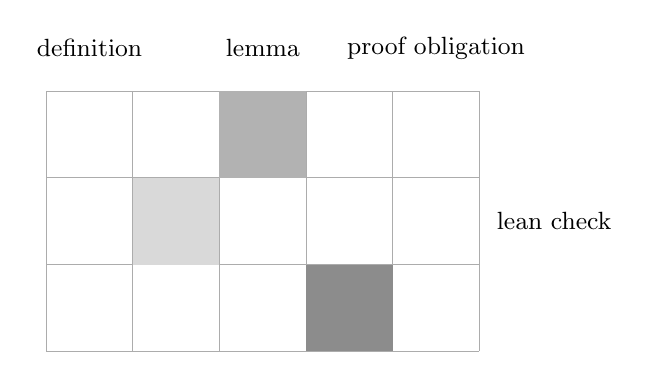
\begin{tikzpicture}[node distance=1.35cm,>=Latex,every node/.style={font=\small}]
\draw[step=1.1cm,gray!65,thin] (0,0) grid (5.5,3.3);
\node[align=center] at (0.55,3.85) {definition};
\node[align=center] at (2.75,3.85) {lemma};
\node[align=center] at (4.95,3.85) {proof obligation};
\node[align=center] at (6.45,1.65) {lean check};
\fill[black!15] (1.1,1.1) rectangle (2.2,2.2);
\fill[black!30] (2.2,2.2) rectangle (3.3,3.3);
\fill[black!45] (3.3,0) rectangle (4.4,1.1);
\end{tikzpicture}
\caption{Lean Formalization Route: evidence matrix of proof dependency pressure 49-1-44}
\label{fig:figure-lean-formalization-route-one}
\end{figure}
The point of the diagram is not decoration; it marks which relation is being proposed and which stronger conclusion is still unavailable.\par
A local clarification is useful here\par
A local clarification is useful here\footnote{In Lean Formalization Route, this note clarifies the reader clarification role of the term and keeps the caveat close to the sentence that needs it.}.\par
The note keeps the caveat near the term without derailing the main sentence.\par
These definitions do not yet prove anything. They only prepare the ground on which proof can begin. If a boundary is still allowed to mean a membrane in one sentence, a legal rule in another, and a sensor limit in a third, Lean has no single object to check. If the chapter says exactly what kind of boundary is in view, Lean can ask whether the proposed consequence really follows.\par
A simple example shows the difference. A lake has a shoreline. A company has a rule about who may approve a payment. Both can be described as having boundaries, but the boundary is not the same kind of thing in the two cases. The shoreline may be represented geometrically, chemically, or hydrologically. The approval rule may be represented as a predicate on actions, a relation among roles, or a constraint in a process. A sentence that says every boundary has an exterior may seem plausible for the lake and misleading for the company. A sentence that says a boundary controls permitted transitions may fit the company better than the shore. Lean cannot resolve this ambiguity by intuition. It requires the object to be declared.\par
This is why formalization belongs neither at the beginning of the theory nor at the end. The reader first needs the ordinary idea: OC describes systems through dimensions of variation, constraints on description, transformations, incompatibilities, and changes in what must be represented. After that, formalization can test selected mathematical claims. It cannot decide whether a living organism, institution, chemical network, or cognitive process truly fits an OC model. That question belongs to interpretation and evidence. Lean can make the mathematical spine inspectable.\par
\section{Axes Before Continua In Lean Formalization Route}
The older literature on self-organization helps explain why this caution is necessary. Prigogine's work on dissipative structures showed that order can be maintained far from equilibrium through flows of energy and matter. Haken's synergetics studied how macroscopic order can arise from coordination among many interacting parts. Nicolis and Prigogine developed a physical and chemical account of nonlinear organization. Kauffman examined autocatalytic networks in which collective structure can arise from the mutual support of reactions. These traditions make emergence, constraint, instability, and organization serious subjects of inquiry. They also show why no single vocabulary is enough. \cite{prigogine_dissipative,haken_synergetics}\par
Each tradition formalizes its world differently. A thermodynamic account may use flows, gradients, and entropy production. A synergetic account may use order parameters and control parameters. A network account may use nodes, edges, closure, and reachability. The same word, organization, can sit near all of them without meaning the same formal thing in each. OC can learn from this situation. A broad theory needs a general language, but the general language becomes scientifically useful only when its translations into particular domains are explicit.\par
The local dependency can now be written without changing the claim it supports.\par
\begin{equation}\label{eq:equation-lean-formalization-route-two}
\operatorname{physicalContinuity}_{11} = \kappa_{K_11}=\frac{b_{K_11}+s_{K_11}}{1+o_{K_11}+q_{K_11}}
\end{equation}
The relation names a local dependency, variable dictionary, and proof/evidence role; it is not a claim-status upgrade.\par
The formula is a restraint on the prose. It names the dependency that the surrounding paragraph is allowed to use.\par
The comparison below gives lean formalization route a set of quantities that can be inspected instead of merely admired.\par
\begin{table}[htbp]
\centering\small
\caption{Lean Formalization Route: observable quantities and counter-pressure 49-2-44}
\label{tab:table-lean-formalization-route-one}
\begin{tabular}{@{}llll@{}}
\toprule
Dataset role & Source type & Replay cue & Reader question \\
\midrule
lean formalization route boundary & 54 units & declared case & fixes what is compared \\
residual pressure & 0.35 & dimensionless & shows unresolved load \\
projection loss & 0.24 & bounded interval & marks lost structure \\
countercase set & 23 cases & review sample & keeps a falsifier visible \\
\bottomrule
\end{tabular}
\end{table}
The table should be read locally: it narrows the comparison without pretending that the wider theory has been settled by a single surface.\par
Lean is useful at the point where translation becomes exact. Suppose OC says that a system occupies a continuum. In one theorem, that continuum might be only a type of possible states. In another, it might be ordered. In another, it might carry a topology or a metric. These are not stylistic differences. An ordered continuum permits claims about before and after, greater and lesser. A metric continuum permits claims about distance. A topological continuum permits claims about neighborhood and continuity. A theorem that needs one structure cannot silently borrow another.\par
The same is true of boundaries. If a boundary is represented as a predicate on states, it divides states into those that satisfy the predicate and those that do not. If it is represented as a relation between descriptions, it concerns how one description is separated from or connected to another. If it is represented as a map into an observational code, it determines what an observer can distinguish. Each choice makes some claims available and others unavailable.\par
Operators require the same care. An operator may be a function that sends every state to a successor. It may be a partial function that sometimes fails. It may be a relation allowing more than one possible successor. It may be a family of transformations indexed by conditions. A theorem about deterministic operators does not automatically apply to nondeterministic systems. A theorem about total operators does not automatically apply where action can fail.\par
Projection is especially delicate because it often loses information. A map from a rich description to a simpler one may preserve some structure and discard other distinctions. That loss is not a defect by itself. Every model selects. The problem begins when a later argument uses a distinction that the projection has already erased. Formalization keeps this visible. If two different states are sent to the same representation, any theorem about the projected object must respect that identification.\par
\section{Operators And Their Burden In Lean Formalization Route}
A small transition model can make the abstract vocabulary less opaque. Imagine a system with four named states: Ready, Strained, Adapted, and Broken. The system begins in Ready. A pressure operator may move it from Ready to Strained. A repair operator may move it from Strained to Adapted. A failure operator may move it from Strained to Broken. The model also has a boundary predicate called Viable. Ready, Strained, and Adapted satisfy Viable. Broken does not. \cite{prigogine_dissipative,haken_synergetics}\par
This is not a model of a particular organism, firm, device, or chemical network. It is a toy structure. Its value lies in its poverty. Because the structure is small, the claims about it can be seen clearly. The states are named. The allowed transitions are named. The boundary predicate is named. The operators are not mysterious powers; they are permitted movements between declared states.\par
The local dependency can now be written without changing the claim it supports.\par
\begin{equation}\label{eq:equation-lean-formalization-route-one}
\operatorname{chemicalPathway}_{11} = \operatorname{support}(c_{11})=P(c_{11})\wedge E(c_{11})\wedge R(c_{11})
\end{equation}
The relation names a local dependency, variable dictionary, and proof/evidence role; it is not a claim-status upgrade.\par
The formula is a restraint on the prose. It names the dependency that the surrounding paragraph is allowed to use.\par
The local dependency can now be written without changing the claim it supports.\par
\begin{equation}\label{eq:equation-lean-formalization-route-three}
\operatorname{cognitiveLoad}_{11} = \operatorname{falsify}(h)=\exists e\in E\,:\,\operatorname{pred}_h(e)\neq\operatorname{obs}(e)
\end{equation}
The relation names a local dependency, variable dictionary, and proof/evidence role; it is not a claim-status upgrade.\par
The formula is a restraint on the prose. It names the dependency that the surrounding paragraph is allowed to use.\par
A small numerical test keeps the abstraction honest at the scale of a single decision.\par
\paragraph{Numerical example.} For lean formalization route, take support=0.59, projection loss=0.13, and 6 open obligations. The bounded score is 0.; the example gives the reader a numeric scale without pretending to be empirical proof.\par
The numbers are deliberately small; their value is pedagogical, not evidential, unless the chapter binds them to a dataset elsewhere.\par
Now add two requirements. The first requirement says that after pressure, the system must preserve Viable. The second says that the system must leave Strained, because remaining there violates a stability condition. In ordinary prose one might call this a contradiction: the current configuration must change, but not every available change preserves the boundary it must keep. In Lean, the word contradiction would not be enough. The formal version would define the active requirements and then define incompatibility as the absence of any allowed successor satisfying them together.\par
Under those definitions, collapse can be stated modestly. Collapse relative to Viable means that from the present state there is no allowed successor that satisfies Viable and the active continuation requirements. In the toy model, if the only available transition from Strained is failure into Broken, then collapse follows relative to the Viable boundary. Lean could check that theorem. It would not have shown that any real system collapsed. It would have shown that the result follows inside this small structure.\par
The same model can illustrate emergence without making it grand. Suppose Strained has two hidden varieties: Strained-with-reserve and Strained-without-reserve. In the original four-state description, both are simply called Strained. The repair operator succeeds from the first and fails from the second. If the original description cannot distinguish those two cases, it cannot state the condition under which repair is possible. A new coordinate, reserve, must be added to represent the difference. In this limited sense, emergence is not a miracle or a slogan. It is the need for an additional descriptive dimension to express a continuation that the old description could not discriminate.\par
A theorem about this miniature might say: if two underlying states are projected into one visible state, and if available continuations differ between them, then the projected description cannot determine the continuation without additional information. That is a useful theorem because it is limited. It speaks about a projection, a pair of states, a transition relation, and a missing distinction. It does not claim that all emergence in nature has been explained.\par
The example also shows why definitions must not be inflated. If collapse were defined as whatever happens when repair fails, a collapse theorem would be easy but uninformative. If emergence were defined as whatever saves the system from collapse, the alternative between emergence and collapse would be built into the vocabulary. The stronger result is the one in which collapse, continuation, projection, and added description are defined independently enough that their relations are worth proving.\par
\section{A Claim Made Inspectable In Lean Formalization Route}
A Lean theorem begins with objects and hypotheses. The surrounding prose may be generous, but the theorem is exact. It says what kinds of things exist in the local setting, what properties they have, and what conclusion follows. This exactness is not merely technical. It protects the reader from equivocation. \cite{prigogine_dissipative,haken_synergetics}\par
Consider the word contradiction. In logic, contradiction may mean that a proposition and its negation are both asserted. In a design problem, it may mean incompatible constraints. In an institution, it may mean rules that cannot be satisfied together in practice. In a scientific model, it may mean a mismatch between prediction and observation. A theorem about incompatible predicates is not a theorem about every one of these cases. If OC uses the same English word across domains, the formal object must be identified each time.\par
The case that follows turns the proposal into a sequence of criticizable moves.\par
\paragraph{Worked case.} In the worked case for lean formalization route, the claim is reduced to a boundary, an observable, a dependency, a numerical cue, and a falsifier. The case is useful only because each move can be criticized separately.\par
The case helps because each step can fail separately, which is exactly what a useful example should permit.\par
The direction of implication also matters. If a theorem says that a certain condition is sufficient for collapse, it does not say that every collapse has that condition. If a theorem says that a defined kind of unresolved incompatibility requires either an enlarged description or failure of continuation, it does not say that every conflict in the world behaves that way. Formal proof is strong precisely where it is bounded.\par
Existence is another source of discipline. A theorem may apply to every system satisfying a list of assumptions even if no interesting example has yet been shown to satisfy them. That does not make the theorem false. It means that its role is formal until examples or domain projections are supplied. In a mature argument, the theorem and the example do different work. The theorem secures consequence. The example shows that the assumptions are inhabited in a relevant way.\par
Hidden assumptions are often the most revealing part of formalization. Does the operator always return a valid state, or can it fail? Are transitions deterministic, or can one state have several successors? Is the boundary fixed, or may it change as the system changes? Is every contradiction decidable? Is every continuation observable? Ordinary prose can pass over these questions because the reader supplies charity. Lean requires the claim to choose.\par
Those choices have scientific weight. Determinism may be appropriate for a simple formal process and inappropriate for a social system. Complete observability may be natural in a toy model and impossible in biology. A fixed boundary may fit a designed protocol and fail for a developing organism. When a later chapter carries a formal result into a domain, the assumptions travel with it. Lean does not decide whether they are empirically justified, but it prevents them from disappearing.\par
This is the proper place of machine checking in a broad theory. It does not make the theory true by force. It makes selected pieces less dependent on rhetorical confidence. A reader need not accept that a theorem follows because the prose sounds disciplined. The objects can be stated, the assumptions inspected, and the derivation checked.\par
\section{What The Formula Does Not Prove In Lean Formalization Route}
Projection is the passage from one description to another. In mathematics it may be a function, an interpretation, a structure-preserving map, or a deliberately lossy translation. In scientific practice it is often the act of representing a complex object in a model that preserves only some features. OC needs projection because it speaks across domains, but projection is also where overclaiming most easily enters. \cite{prigogine_dissipative,haken_synergetics}\par
Return to the contrast between a physical boundary and an institutional boundary. A laboratory membrane may separate concentrations, regulate flows, and produce measurable gradients. An institutional rule may separate authorized from unauthorized actions, create incentives, and determine valid transitions in a workflow. Both can be modeled with predicates or relations, but the projection from domain to formal object preserves different things. A membrane does not approve an invoice. A rule does not diffuse a molecule. If a theorem concerns reachability under a predicate, both may instantiate it. If a theorem concerns conservation across a physical interface, the institutional case has not been reached.\par
This is why resemblance of vocabulary is never enough. Dissipative structures, synergetic systems, autocatalytic networks, and OC configurations may all involve order, constraint, and transformation. Yet each comes with its own primitives. The productive comparison is not that they are secretly the same. It is that each shows a way in which organization depends on conditions, and each forces the theorist to specify which conditions matter.\par
A projection must therefore say what is preserved. It may preserve reachability: if one state can follow another in the domain, the projected state can follow the projected state in the model. It may preserve boundary membership: if a domain state satisfies the relevant constraint, its formal image satisfies the formal predicate. It may preserve incompatibility: if two requirements cannot be jointly satisfied in the domain representation, their formal counterparts cannot be jointly satisfied either. Each preservation claim is separate.\par
It must also say what is not preserved. A simplified organizational model may ignore emotion, history, informal power, and tacit knowledge. A chemical network model may ignore spatial heterogeneity. A cognitive model may ignore physiology. These omissions do not automatically invalidate the model. They become serious only when conclusions depend on the omitted material.\par
Lean can express some of these preservation claims cleanly. It can check a bridge theorem saying that a projection carries one relation into another. It can check that a lossful map cannot recover distinctions it identifies. It can check that a theorem about the target structure applies only when the required properties are present. It cannot decide that the projection is scientifically adequate. That decision belongs to modeling practice, evidence, and domain expertise.\par
The modesty of this division is a strength. It allows formal claims to be strong without pretending to be empirical claims. A bridge theorem may be exact and still limited. A domain projection may be plausible and still open to challenge. Evidence may support a projection in one domain and not another. Keeping these differences visible makes the theory harder to inflate and easier to test.\par
\section{The First Formal Move In Lean Formalization Route formaliz}
OC's broadest hypothesis can now be stated without asking it to carry more than it can bear. In its general form, the hypothesis says that an unresolved structured incompatibility presses a configuration toward one of two outcomes: an enlarged description that can represent the missing distinction, or a failure of coherent continuation under the old description. In the language used here, the alternatives are emergence and collapse. \cite{prigogine_dissipative,haken_synergetics}\par
As a statement about all possible systems, this is not something Lean can simply prove. The world is not a Lean file. Nature, institutions, organisms, and cognitive processes do not arrive already packaged as declared types with checked predicates. What Lean can do is examine fragments of the hypothesis under explicit models. It can show, for example, that in a transition system with defined continuation, resolution, boundary preservation, and dimension extension, certain alternatives exhaust the cases. It can show that a projected description loses the ability to determine a continuation when it erases the relevant distinction. It can show that collapse follows when no allowed successor preserves active requirements.\par
These are not small results because they are conditional. Conditional results are the normal form of mathematics. Their value depends on the clarity and usefulness of the conditions. A theorem whose assumptions are few, visible, and interpretable can support later argument. A theorem whose assumptions are numerous, hidden, or tailored to force the desired conclusion cannot carry much weight.\par
The self-organization traditions sharpen this point. Prigogine's dissipative structures do not merely say that order appears; they specify physical conditions under which ordered structures can be maintained far from equilibrium. Haken's synergetics does not merely celebrate coordination; it studies how order parameters can govern collective behavior. Kauffman's autocatalytic networks do not merely name emergence; they examine closure and mutual production in networks. The lesson for OC is that general language earns seriousness by becoming selective. It must say which structures are present, which transitions are allowed, which constraints are active, and which forms of evidence would matter.\par
Lean contributes to that selectivity. It can show when the central alternative has been made too easy by definition. It can show when the conclusion does not follow without an added assumption. It can show when a theorem proves only one direction. It can show when a result depends on determinism, decidability, or fixed boundaries. Each discovery narrows the claim into something more honest.\par
There is also a positive gain. Once a theorem is checked, later chapters can refer to it without rebuilding the derivation in prose. The reader can ask a sharper question: does the present domain satisfy the theorem's assumptions? If the answer is yes, the formal consequence is available. If the answer is no, the theorem remains nearby but unused. This is how formalization supports a scientific monograph without replacing science.\par
\section{Axes Before Continua In Lean Formalization Route formaliz}
Some claims should remain outside Lean-backed use until the missing work has been done. An undefined term is the simplest case. If emergence, collapse, contradiction, boundary, or projection has no formal counterpart in the theorem at hand, no checked result should be invoked for that sentence. The prose may explain an idea, but it cannot borrow the authority of a proof that does not exist. \cite{prigogine_dissipative,haken_synergetics}\par
A domain leap is equally dangerous. A theorem about the four-state transition model cannot be carried into thermodynamics, organizational life, cognition, or biology because the same words appear. The bridge requires a projection that says how the domain object is represented and which assumptions survive the translation.\par
A hidden axiom is more subtle. If a proof depends on every transition having a successor, every contradiction being decidable, or every relevant boundary remaining fixed, the prose must disclose that dependency before the result is used. These assumptions may be harmless in one setting and false in another. Their visibility is part of the result.\par
A definitional shortcut weakens a theorem even when the proof checks. If unresolved contradiction is defined as a condition that necessarily produces either emergence or collapse, then a theorem deriving emergence or collapse has little content. The useful theorem is one in which the alternatives arise from definitions that can be understood independently.\par
Equivocation across meanings must also be avoided. A formal contradiction between predicates does not automatically describe psychological tension, institutional conflict, or experimental anomaly. A set-theoretic boundary does not automatically describe a thermodynamic interface. A projection that preserves one relation does not preserve every relation. The same vocabulary can guide comparison, but the formal claim must stay attached to its object.\par
The most important limit is empirical substitution. A Lean theorem cannot replace observation, simulation, experiment, archival evidence, or domain-specific comparison. It can clarify the model being tested. It can prevent internal mathematical confusion. It can make assumptions inspectable. It cannot supply missing data.\par
This limit is not a concession made after the fact. It is the condition under which formalization remains credible. A theory that knows where its proofs stop is stronger than one that treats formal language as a universal seal. OC can propose a general operational vocabulary while still requiring, in each domain, a separate account of representation and evidence.\par
\section{Operators And Their Burden In Lean Formalization Route formaliz}
The public role of Lean in OC is therefore narrow and important. It secures conditional consequence. It can show that a conclusion follows from declared objects and assumptions. It can reveal missing assumptions, prevent equivocation, distinguish sufficient from necessary conditions, and expose when a desired theorem has been built into a definition. \cite{prigogine_dissipative,haken_synergetics}\par
It cannot show that a real system satisfies the model. It cannot transform resemblance to self-organization literature into validation. It cannot make a global scientific hypothesis true by checking a local mathematical fragment. A theorem about an abstract operator is not a measurement. A theorem about collapse in a transition system is not evidence that a biological, chemical, institutional, or cognitive system has collapsed.\par
The central distinction is simple but demanding: formalization secures consequence, not instantiation. If the declared structure holds, the checked conclusion follows. Whether the declared structure fits a domain is a further question. Whether the evidence supports that fit is another question still.\par
This distinction prepares later use of formal material. When a chapter states a mathematical claim, the reader can ask what has been defined. When it invokes a theorem, the reader can ask which assumptions are active. When it moves into a domain, the reader can ask what the projection preserves and what it loses. When it discusses evidence, the reader can ask whether the model has actually met the world.\par
Lean Formalization Route is not the place where OC becomes empirically established. It is the place where selected parts of its mathematical structure become inspectable. The value of that inspection lies in restraint. It makes some claims stronger by making them smaller, clearer, and harder to smuggle across boundaries they have not earned.\par
\chapter{Finite Semantic Checks}
\section{The Local Problem In Finite Semantic Checks}
A sentence can fail before it is false. It can fail because its words do too much work at once, because a term that was precise in one setting becomes loose in another, or because a comparison borrows the confidence of a field without carrying over the conditions that made the confidence legitimate. This kind of failure is common in ambitious theoretical language. A market adapts, a cell adapts, a climate regime adapts. The verb is familiar, but familiarity is not stability. In the cell, adaptation may name a metabolic response, a regulatory change, or survival across a perturbation. In the market, it may name price adjustment, strategic learning, or institutional redesign. In the climate case, it may name the reorganization of coupled atmospheric and oceanic processes, or it may name human responses to environmental change. The same verb has crossed domains faster than its meaning has been accounted for. \cite{haken_synergetics,nicolis_prigogine_selforg}\par
A finite semantic check is a bounded inspection of that crossing. It asks whether a statement still says the same kind of thing after its terms have been placed inside the vocabulary of the Ontology of Continua. The word finite is not a concession to convenience. It is an epistemic restraint. The check refuses the temptation to inspect everything at once: every system, every interpretation, every possible observation, every neighboring theory. It chooses a bounded expression, such as a claim, a definition, a proposed relation, a projected comparison, or a candidate formal statement, and asks whether the meanings assigned there can be held still long enough to be examined.\par
The next diagram slows the argument down just enough to show how finite semantic checks is being organized.\par
\begin{figure}[htbp]
\centering
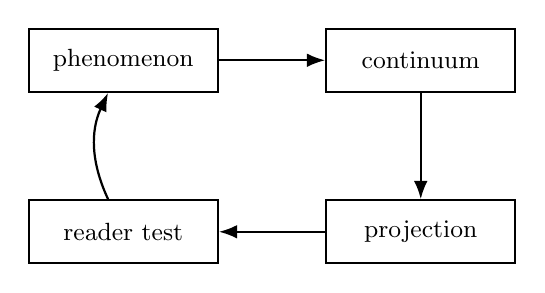
\begin{tikzpicture}[node distance=1.35cm,>=Latex,every node/.style={font=\small}]
\node[draw,thick,align=center,minimum width=2.4cm,minimum height=0.8cm] (a) {phenomenon};
\node[draw,thick,align=center,minimum width=2.4cm,minimum height=0.8cm,right=of a] (b) {continuum};
\node[draw,thick,align=center,minimum width=2.4cm,minimum height=0.8cm,below=of b] (c) {projection};
\node[draw,thick,align=center,minimum width=2.4cm,minimum height=0.8cm,left=of c] (d) {reader test};
\draw[->,thick] (a) -- (b);
\draw[->,thick] (b) -- (c);
\draw[->,thick] (c) -- (d);
\draw[->,thick,bend left=25] (d) to (a);
\end{tikzpicture}
\caption{Finite Semantic Checks: phase diagram of conceptual dependency pressure 50-1-45}
\label{fig:figure-finite-semantic-checks-one}
\end{figure}
The point of the diagram is not decoration; it marks which relation is being proposed and which stronger conclusion is still unavailable.\par
A local clarification is useful here\par
A local clarification is useful here\footnote{In Finite Semantic Checks, this note clarifies the reader clarification role of the term and keeps the caveat close to the sentence that needs it.}.\par
The note keeps the caveat near the term without derailing the main sentence.\par
The word semantic is equally important. The check concerns meaning before measurement, meaning before proof, meaning before cross-domain transfer. It does not settle whether a natural system behaves as described. It does not establish a mathematical theorem. It does not supply empirical evidence. It prepares the conditions under which those later efforts can have a determinate target. Without such preparation, data may appear to support one claim while actually addressing another, and formal symbols may appear exact while inheriting ambiguities from the prose that introduced them.\par
OC Core 1.4 uses a small group of terms for comparing systems without treating them as identical. A continuum is a dimension of description along which variation can be represented without pretending that every point on it is already measured. A boundary is the distinction that makes some variation count as internal to the described configuration and some variation count as external, adjacent, or excluded. An operator is an action, transformation, rule, constraint, or mapping that changes a configuration or reveals how it can change. A contradiction is a structured incompatibility within the described configuration, not merely an argument between people or a clash between sentences. Emergence names, in OC vocabulary, the appearance of a new dimension of description when the existing arrangement cannot adequately carry what has appeared. Collapse names the loss of coherence of a configuration under an unresolved incompatibility. These are conceptual roles, not empirical victories by themselves.\par
Because the terms are broad, they can become careless unless they are kept answerable. A finite semantic check asks what job each term is doing in a particular sentence. If a claim says that a contradiction gives rise to a new dimension, the check asks what counts as the contradiction, what counts as the prior descriptive space, what counts as the new dimension, and what alternative outcome would count as collapse or ordinary adjustment. If a claim says that an operator acts on a continuum, the check asks what is varying, where the boundary is drawn, and whether the operation changes the system, the description, or the observer's classification. These questions do not diminish the theory. They give it handles. They prevent the theory from saying everything at once.\par
Several supporting terms will matter in what follows. A proof route is the path by which a claim moves from public prose toward mathematical inspection. It is a route of responsibility, not a declaration that the claim is already proved. A formalization check asks whether the prose has become precise enough to offer a determinate target for notation, theorem-like statements, computation, or machine-checked expression. Term fixation means assigning an important word a stable role within the bounded claim under inspection. Relation fixation means stating how those fixed terms stand to one another. Type discipline means keeping unlike things from sliding into one another: a system is not the same as a description of a system, a boundary is not the same as measurement error, and a classification rule is not the same as a natural force. These phrases are simple in purpose. They name the work by which meaning becomes inspectable.\par
\section{The Necessary Distinction In Finite Semantic Checks}
The movement begins in ordinary speech because ordinary speech is where theoretical ambition usually starts. A group of people says that a plan is failing. A biologist says that a network reorganizes under stress. An economist says that an institution adapts. A physicist describes order sustained by flows through a system. Each sentence may be useful. Each also carries a danger. The words feel available before their commitments have been specified. \cite{haken_synergetics,nicolis_prigogine_selforg}\par
Imagine a room of people coordinating around a plan. At first the plan works because the group shares several tacit distinctions: who decides, what counts as success, which tasks belong inside the group, and which disturbances can be ignored. Then something changes. A deadline is cut in half, a necessary resource disappears, or two goals that looked compatible begin to compete. The group may adjust within the old arrangement. It may redistribute effort, sequence tasks differently, or reduce scope while preserving the same measure of success. In OC language, that would be variation inside an existing continuum.\par
The local dependency can now be written without changing the claim it supports.\par
\begin{equation}\label{eq:equation-finite-semantic-checks-two}
\operatorname{technologyCoupling}_{12} = C_{\mathrm{unres}}=\min_{\pi\in\Pi}\|B(x)-B(\pi x)\|
\end{equation}
The relation names a local dependency, variable dictionary, and proof/evidence role; it is not a claim-status upgrade.\par
The formula is a restraint on the prose. It names the dependency that the surrounding paragraph is allowed to use.\par
The comparison below gives finite semantic checks a set of quantities that can be inspected instead of merely admired.\par
\begin{table}[htbp]
\centering\small
\caption{Finite Semantic Checks: observable quantities and counter-pressure 50-2-45}
\label{tab:table-finite-semantic-checks-one}
\begin{tabular}{@{}llll@{}}
\toprule
Falsifier & Trigger & Expected failure & Consequence \\
\midrule
finite semantic checks boundary & 57 units & declared case & fixes what is compared \\
residual pressure & 0.42 & dimensionless & shows unresolved load \\
projection loss & 0.35 & bounded interval & marks lost structure \\
countercase set & 24 cases & review sample & keeps a falsifier visible \\
\bottomrule
\end{tabular}
\end{table}
The table should be read locally: it narrows the comparison without pretending that the wider theory has been settled by a single surface.\par
A different response changes the description itself. The group introduces priority ranking where none existed before. It creates a new role with authority to resolve tradeoffs. It changes the measure of progress from task completion to risk reduction. In that case, the group may need a new dimension of description to explain what it is doing. The old task-allocation space is no longer enough. The point is modest: this is a toy case for semantics, not evidence that organizations, cells, and physical systems instantiate one literal structure. It shows how a vocabulary can be disciplined before it travels.\par
The same example also shows collapse in a limited sense. The group may lose the shared plan as a common object of coordination. People continue acting, but the configuration that made their actions part of one plan no longer holds together. That is not the end of the people, the end of work, or the failure of every possible description. It is the loss of coherence of the configuration under description. A finite semantic check keeps that limit visible. It asks which configuration is said to collapse, under which incompatibility, and relative to which boundary.\par
The movement from the room to a technical domain must be earned. In a biological case, the continuum might describe metabolic states, regulatory states, or network connectivity. The boundary might separate a modeled reaction system from its chemical environment. The operator might be a perturbation, a reaction rule, a selection condition, or a feedback relation. The contradiction might be an unsatisfied joint requirement within the model. Emergence and collapse would have to be stated with equal care. The words cannot simply be carried from the meeting room to the cell.\par
This is where finite checks enable rather than merely restrict. They make comparison possible without flattening the compared domains. The meeting room can teach the grammar of assignment: object, boundary, variation, operation, incompatibility, revision. Biology can then receive that grammar only where its own objects and relations support it. A failed transfer is informative. It shows that the resemblance was verbal, or that the boundary was wrong, or that the operator was really an observer's description. Such failures are valuable because they leave the theory smaller, clearer, and more available for correction.\par
Neighboring scientific traditions matter here because they show how much discipline strong general language requires. Haken's synergetics is relevant not as a source of authority for OC, but as a reminder that collective order becomes scientifically serious when variables and order parameters are specified. Nicolis and Prigogine are relevant because nonequilibrium self-organization depends on flows, boundaries, and maintained conditions rather than on a vague image of spontaneous pattern. Kauffman's work on autocatalytic sets is relevant because mutual enabling becomes more than a metaphor when components and catalysis relations are named. RAF networks sharpen the same lesson by specifying reflexively autocatalytic and food-generated conditions for reaction systems. These traditions are not interchangeable. They locate a problem OC must face in its own language: powerful comparisons need explicit conditions.\par
\section{Operators And Their Burden In Finite Semantic Checks}
A claim that may later become formal has to pass through prose first. Mathematical notation can clarify, compress, and test relations, but it cannot rescue a public claim whose object changes while the reader is trying to follow it. The proof route begins when a sentence becomes stable enough to ask what a formal version would have to preserve. \cite{haken_synergetics,nicolis_prigogine_selforg}\par
Term fixation is the first practical movement, although it need not be announced as a procedure. A reader can be able to tell what each important term names in the bounded claim. If the claim concerns a continuum, the relevant dimension of variation has to be visible. If it concerns a boundary, the distinction of inclusion or relation has to be visible. If it concerns an operator, the transformation or rule has to be visible. If it concerns contradiction, the structured incompatibility has to be visible. If it invokes emergence or collapse, the sentence has to distinguish a new dimension of description from ordinary change, and loss of coherence from ordinary ending.\par
The local dependency can now be written without changing the claim it supports.\par
\begin{equation}\label{eq:equation-finite-semantic-checks-one}
\operatorname{agencyChoice}_{12} = \Delta d=\operatorname{rank}(A_{\mathrm{new}})-\operatorname{rank}(A_{\mathrm{old}})
\end{equation}
The relation names a local dependency, variable dictionary, and proof/evidence role; it is not a claim-status upgrade.\par
The formula is a restraint on the prose. It names the dependency that the surrounding paragraph is allowed to use.\par
The local dependency can now be written without changing the claim it supports.\par
\begin{equation}\label{eq:equation-finite-semantic-checks-three}
\operatorname{aiAlignmentProxy}_{12} = P_{\mathrm{collapse}}=\sigma(\alpha R-\beta S-\gamma M)
\end{equation}
The relation names a local dependency, variable dictionary, and proof/evidence role; it is not a claim-status upgrade.\par
The formula is a restraint on the prose. It names the dependency that the surrounding paragraph is allowed to use.\par
A small numerical test keeps the abstraction honest at the scale of a single decision.\par
\paragraph{Numerical example.} For finite semantic checks, take support=0.42, projection loss=0., and 1 open obligations. The bounded score is 0.180; the example gives the reader a numeric scale without pretending to be empirical proof.\par
The numbers are deliberately small; their value is pedagogical, not evidential, unless the chapter binds them to a dataset elsewhere.\par
Relation fixation follows naturally. A sentence may define its terms and still leave their relations obscure. Does the operator act inside a continuum, between continua, across a boundary, or on the boundary itself? Does the contradiction arise from two operators, from a boundary condition, from an attempted projection, or from an impossible joint requirement? Does emergence mean that a new continuum becomes necessary for description, or that a previously latent continuum becomes active within the model? Does collapse mean the destruction of a physical system, the failure of a description, the breakdown of a level, or the failure of a projection? These differences determine what a later theorem, simulation, or counterexample would have to address.\par
Exclusion gives the claim its edges. A useful statement tells the reader what does not count. If every unresolved tension is called contradiction, contradiction becomes another name for difficulty. If every new label is called a new dimension, emergence becomes bookkeeping. If every prediction failure is called collapse, collapse describes the observer's disappointment rather than the configuration's loss of coherence. Finite checks protect the ability to say: this case fits, this nearby case does not, and the difference matters.\par
Only after those assignments does minimal formal restatement become useful. The restatement may remain verbal, or it may be symbolic, diagrammatic, computational, or eventually machine checked. At the finite stage, its virtue is smallness. It might show that a claim uses one term in two incompatible ways. It might expose a missing boundary. It might reveal that a descriptive operation has been treated as a cause. It might translate a sentence into a finite set of named roles and relations, then show that the assignment is coherent or incoherent. Such work is not a grand demonstration. It clears the ground on which a demonstration could later stand.\par
The analogy with autocatalytic network theory is useful because it shows how a broad intuition can become more accountable. The idea of mutually enabling reactions is suggestive. Its scientific value increases when components, catalysis relations, closure conditions, and food sets are specified. RAF theory does not prove OC, and OC does not inherit RAF results by resemblance. The methodological lesson is narrower and stronger: a vocabulary becomes more available to science when attractive general words are tied to finite constraints.\par
A failed finite check is therefore not a failed world. It is a failed formulation. The phenomenon may remain real. The intuition may remain promising. The research direction may still be worth pursuing. What fails is the current sentence's right to carry later weight. The term can be narrowed. The boundary can be redrawn. The projection can be withdrawn. The operator can be split into two operators. The route remains open, but the claim must return to the point where its meaning became unstable.\par
This slower pace is especially important for OC's treatment of contradiction, emergence, and collapse. OC vocabulary permits the hypothesis that a structured incompatibility may require a new dimension of description or may coincide with the loss of coherence of a configuration that cannot resolve it. That is a conceptual possibility inside the framework, not a settled empirical law. A finite semantic check asks what would have to be assigned before the hypothesis could be used responsibly: the existing configuration, the active boundary, the incompatible requirements, the candidate new dimension, and the condition under which coherence is lost. The claim becomes stronger by becoming more answerable.\par
\section{An Objection Worth Keeping In Finite Semantic Checks}
Consider a deliberately bounded biological sentence: in a modeled reaction network, a nutrient shift creates contradiction and the network emerges into a new continuum. The sentence has the rhythm of theory, but at first it is too quick. A finite semantic check slows it down until the reader can see what would be examined. \cite{haken_synergetics,nicolis_prigogine_selforg}\par
The object is not all biology. It is a specified model of a reaction network. Let the model contain a finite set of chemical species, a finite set of reactions, and a rule stating which reactions are available under a given nutrient condition. The boundary is the modeled reaction system plus a declared food set supplied from the environment. That boundary matters because a reaction unavailable inside the network may become available if the environment is quietly changed. The check therefore fixes the boundary before judging the claim.\par
The case that follows turns the proposal into a sequence of criticizable moves.\par
\paragraph{Worked case.} In the worked case for finite semantic checks, the claim is reduced to a boundary, an observable, a dependency, a numerical cue, and a falsifier. The case is useful only because each move can be criticized separately.\par
The case helps because each step can fail separately, which is exactly what a useful example should permit.\par
The continuum is the set of viable internal flux configurations under the original nutrient condition, represented at the level the model uses. Viability here has a bounded meaning: the network can maintain the modeled production of a required species while respecting the reaction constraints. The operator is the nutrient shift, represented as a change in the food set or in the availability of one input species. This operator acts on the boundary condition of the modeled network. It is not yet a cause in real biology beyond the model, and it is not the continuum itself.\par
The word contradiction now needs repair. Chemical reactions do not encounter contradiction as propositions do. A better assignment is this: after the nutrient shift, the model imposes two requirements that cannot be jointly satisfied inside the original reaction closure. The network must maintain production of a required species, and it must do so without an input that the original closure requires. If the model shows that no flux configuration in the original continuum satisfies both requirements, then the contradiction is not a mood of difficulty. It is a structured incompatibility among declared requirements and available reactions.\par
The candidate emergence claim also needs narrowing. A new continuum does not appear merely because the observer adds a label. It appears, in this bounded OC sense, only if describing viable configurations now requires a dimension absent from the original state space. Suppose the model is extended by adding a class of alternative reactions that use a different input and produce an intermediate not represented in the original description. If viability can be restored only by tracking that intermediate and the alternative reaction class, then the revised description may require a new dimension. The finite check has not shown that a real organism evolved such a route. It has shown that the modeled claim has a coherent semantic form.\par
Near-misses clarify the result. If the original network already contained a dormant alternative reaction and the nutrient shift merely changed its rate, the case may be activation within the existing continuum rather than emergence of a new one. If the observer adds a new axis only for convenience while the old state space still represents the viable configurations adequately, the novelty belongs to the description, not necessarily to the modeled organization. If the nutrient is removed from outside and no internal incompatibility is specified, the result may be ordinary failure under changed conditions rather than collapse under contradiction. If the network ceases producing the required species because the model was underspecified, the failure belongs to the model, not to the network.\par
The sentence can now be revised. A defensible version would read: within a specified finite reaction-network model, a nutrient shift changes the food-set condition so that the original reaction closure cannot satisfy the declared viability requirement; if restoring viability requires adding and tracking a previously absent class of reactions and intermediates, the model requires a new continuum of description for the viable configurations. This is still a modest claim. Its modesty is its strength. It says what the object is, where the boundary lies, what varies, what operator acts, what incompatibility is present, what near cases are excluded, and what revision follows from failure.\par
The check also leaves open the later scientific questions. A biologist may ask whether the model represents any measured system. A mathematician may ask whether the impossibility result follows from the stated reaction constraints. A computational scientist may ask whether the search over configurations was complete. A philosopher of science may ask whether the new dimension belongs to the system or to the model. Each question now has a target. The finite semantic check has made disagreement more precise.\par
\section{The Result Of This Passage In Finite Semantic Checks}
Finite semantic checks block sentences that ask for more authority than their construction can bear. This blocking is not merely negative. It creates the positive space in which smaller, clearer claims can be compared, corrected, and formalized. \cite{haken_synergetics,nicolis_prigogine_selforg}\par
Pure synonymy is one common failure. If the organization changed becomes the continuum reconfigured, nothing has been gained unless the continuum and reconfiguration are specified. If the plan failed becomes the configuration collapsed, the new phrase must identify the configuration and the collapse condition. A vocabulary that only renames familiar events has become ornamental.\par
Domain smuggling is another. Autocatalysis has technical meaning in chemistry and network theory; it cannot be carried into social or cognitive cases merely because mutual reinforcement appears there. Synergetic order parameters belong to a particular theoretical setting; not every summary variable in another domain is an order parameter in that sense. Nonequilibrium self-organization involves relations among flows, constraints, structures, and environments; not every organized pattern maintained by effort becomes a nonequilibrium structure in the technical sense. OC may compare these languages, but comparison must preserve the conditions that make each language disciplined.\par
Observer substitution is subtler. A new dimension of description may arise because the observer notices an axis that had previously been ignored. That can be a legitimate advance in modeling. It is not automatically emergence in the described system. If a researcher adds a variable to a spreadsheet, the system has not necessarily reorganized. If an analyst introduces a new category, the population described has not necessarily changed. If a mathematician refines a definition, the mathematical object may become clearer without any physical system undergoing transformation. The check asks where the novelty occurs.\par
Contradiction inflation also has to be resisted. Ordinary conflict, uncertainty, tradeoff, surprise, error, and complexity are not automatically contradiction. A contradiction in OC requires structured incompatibility within the configuration as described. Two people disagreeing is not enough. Two measurements differing is not enough. A system being hard to predict is not enough. Even a severe constraint is not enough if the configuration can absorb it within the existing dimensions. The check asks whether the incompatibility is internal to the relevant description and whether it survives clarification, parameter adjustment, and boundary correction.\par
Collapse inflation follows the same pattern. Not every end is collapse. A process can stop because its task is complete. A structure can disappear because external conditions changed. A model can fail because it was poorly built. A population can decline because a resource is removed. Some of these cases may involve collapse under a carefully stated OC description, but the word has to earn its place. Collapse requires the loss of coherence of the configuration under the relevant unresolved incompatibility.\par
Emergence inflation is equally tempting. Not every novelty is emergence. A new label, measurement, input, or arrangement may or may not require a new dimension of description. The question is whether the previous descriptive space can represent the new organization without distortion. Haken's work offers one historical reminder that collective behavior may invite a different level of description, but OC cannot turn that reminder into a universal license. The work remains local: what changed, what description failed, what new dimension became necessary, and under what boundary?\par
Formal displacement is blocked as well. A text can point toward mathematics to create confidence before showing what is being formalized. A proof may be valid inside its premises while missing the public claim. A simulation may explore a model while leaving the interpretation of the model unsettled. A dataset may constrain a claim while the terms of the claim remain unstable. The finite check insists that the public sentence and the formal or empirical object be related before authority moves between them.\par
Totalizing projection is the broadest danger. A projection is a controlled movement from one descriptive setting to another. It is not a declaration that all systems are the same. A continuum in cognition is not automatically a continuum in chemistry. A boundary in a political institution is not automatically a membrane. An operator in a formal model is not automatically a force in nature. Projection must say what relation is preserved and what is left behind. A finite semantic check can approve a narrow transfer while rejecting a broad one, and that selectivity is what makes comparison useful.\par
\section{The Local Problem In Finite Semantic Checks checksS0}
The strength of a finite semantic check lies in its size. It does not try to make the entire theory secure. It makes one bounded claim answerable. That answerability has several positive effects. It gives later formal work a cleaner target. It gives empirical work clearer terms of measurement or comparison. It gives criticism a definite object. It allows cross-domain language to move without pretending that resemblance is identity. \cite{haken_synergetics,nicolis_prigogine_selforg}\par
The word finite also protects against totalizing language. A theory that speaks across domains can easily drift toward sentences so large that no example can discipline them. Finite checks reverse that drift. They force claims into bounded assignments: this object, this boundary, this continuum, this operator, this incompatibility, this possible revision. The result is not timid. It is inspectable. A large synthesis built from inspectable pieces is more serious than a sweeping sentence that cannot be corrected because no one can say exactly what would count against it.\par
Type discipline supports the same aim. The prose must keep systems, descriptions, models, measurements, classifications, and causes distinct unless it argues for their relation. A system may be represented by a model, but the model is not the system. A boundary may be drawn for analysis, but that analytic boundary is not automatically a physical interface. An operator may describe a transformation in a formal space, but it is not thereby a natural cause. A contradiction may be expressed in language, but the relevant incompatibility may belong to a modeled configuration rather than to a set of propositions. Keeping these types distinct does not impoverish the theory. It prevents false depth.\par
Modal discipline matters just as much. It is one thing to say that a structured incompatibility may require a new dimension of description. It is stronger to say that it must. It is stronger still to say that a measured system did. The difference among may, must, and did is not stylistic. It marks the scientific status of the sentence. OC can describe a conceptual route from contradiction toward emergence or collapse, but conceptual availability is not empirical confirmation. A finite semantic check keeps the modal force visible.\par
The same discipline improves the use of formal languages and proof assistants. A machine-checked statement can confirm that a formal object follows from stated premises. It cannot by itself confirm that the formal object captures the public claim. If contradiction is represented as inconsistency in a logical calculus, the text must explain how that representation relates to structured incompatibility in a system description. If boundaries are represented as sets, the text must say what that representation preserves and what it loses. If time is abstracted away, the later prose cannot rely on temporal dynamics as though they had been included.\par
Finite semantic checks therefore respect formality by refusing to misuse it. They keep prose from borrowing unearned formal confidence, and they keep formal work from being asked to solve a problem of meaning that belongs earlier. A critic can then ask precise questions: Was the boundary chosen well? Was the operator defined correctly? Was the incompatibility genuine? Was the modal force too strong? Did the projection exceed the case? These are not hostile questions from outside the project. They are the form a serious conversation takes once meaning has become inspectable.\par
The result is a cleaner kind of ambition. OC may still compare biological, cognitive, social, formal, and physical descriptions. It may still ask whether contradiction, emergence, collapse, boundary, operator, and continuum can support a shared language of analysis. But each comparison has to arrive through bounded claims. The theory earns breadth by surviving finite checks, not by rising above them.\par
\section{The Necessary Distinction In Finite Semantic Checks checksS0}
For a first-time reader, finite semantic checks explain how OC can be ambitious without becoming a metaphor engine. The phrase is severe because the danger is real. A metaphor engine produces motion without accountability. It turns every conflict into contradiction, every novelty into emergence, every ending into collapse, every influence into an operator, and every difference into a boundary. The sentences become impressive precisely because they are hard to test. Finite checks reverse that tendency by making the impressive sentence smaller until its parts can be seen. \cite{haken_synergetics,nicolis_prigogine_selforg}\par
The room of people around a failing plan gives the simplest picture. A shared arrangement encounters a disturbance. The group may adjust within the existing task space, introduce a new priority dimension, or lose the shared plan as a coherent object of coordination. The example proves nothing about nature. It teaches the grammar of inspection. Once that grammar is learned, it can be carried carefully into technical cases, where the terms must be assigned according to the domain rather than according to the charm of the analogy.\par
The biological reaction-network case shows the fuller movement. A loose sentence about a network meeting contradiction becomes a bounded model claim about species, reactions, a food set, a viability requirement, a nutrient shift, an unsatisfied closure condition, and a possible new dimension of description. The revision is less dramatic than the original sentence, but it is more useful. It can be questioned. It can be modeled. It can be rejected. It can be connected to evidence if the evidence exists. It can fail without taking the entire theory down with it.\par
This is the main public value of the check. It creates cleaner failures. A theory that cannot fail locally tends to fail globally, because criticism has no smaller place to enter. Finite semantic checks make local failure possible. A boundary assignment can fail. A term can fail. A projection can fail. A formalization target can fail. Such failures are not embarrassments to be hidden. They are the means by which the language becomes more exact.\par
They also create clearer successes. When a finite check passes, the result is not triumph but readiness. The claim is ready for more demanding treatment: a formal restatement, a mathematical conjecture, a simulation, a comparison with data, a domain-specific analysis, or a sharper objection. Later work may still fail. The boundary may turn out to be poorly chosen, the operator too crude, the model too artificial, the empirical comparison too weak. But the object of success or failure can now be named.\par
The likely objection is that such checks are too small to matter. They do not produce data. They do not settle whether OC is true. They do not show that any given physical, biological, cognitive, or social system has followed the route the vocabulary makes available. That objection is right about their limits and wrong about their importance. Scientific claims fail not only when evidence defeats them, but also when their terms cannot be held steady long enough for evidence, mathematics, or criticism to touch them.\par
Another objection is that semantic restraint may weaken the sweep of the project. If every term must be introduced, every boundary named, and every projection limited, the prose may seem to lose some of its reach. But reach without control is not explanation. OC can still make large claims. It simply has to assemble them from smaller claims whose meanings can be inspected. The finite check is not the enemy of synthesis. It is the condition under which synthesis can remain answerable.\par
The handoff to later work is therefore straightforward. Definitions, theorem-like statements, proof sketches, computational models, empirical comparisons, domain projections, objections, and limits all depend on sentences whose meanings have not drifted away from them. A finite semantic check does not guarantee that those later efforts will succeed. It guarantees something more basic and more necessary: when a later claim succeeds or fails, the object of success or failure can be named. That is the minimum condition for a public scientific monograph that compares systems without erasing their differences.\par
\part{domain projections}
\chapter{K0 Physical Projection}
\section{The Domain Enters In Physical Projection}
Ordered Continuum, abbreviated OC, begins its physical projection from a plain observation: physical systems do not merely contain things; they maintain, lose, shift, or transform arrangements. A candle flame persists while fuel, oxygen, heat, and air movement remain within a workable range. A whirlpool holds a visible form while water continually passes through it. A crystal keeps a rigid pattern because local molecular constraints settle into a repeating geometry. These examples are not the same kind of system, yet each raises the same first question: what makes a bounded physical arrangement count as one continuing configuration rather than a loose inventory of parts? \cite{nicolis_prigogine_selforg,kauffman_autocatalytic}\par
K0 names the most minimal physical level of that question. The name is deliberately austere. It does not announce a new physics, a hidden substance, or a master equation beneath existing science. It marks the first projection of OC vocabulary into material systems. A projection is a disciplined translation from a general set of terms into a particular domain. In K0, the domain is physical configuration: matter, energy, constraints, thresholds, flows, reactions, forces, and the conditions under which an arrangement persists or fails.\par
The next diagram slows the argument down just enough to show how physical projection is being organized.\par
\begin{figure}[htbp]
\centering
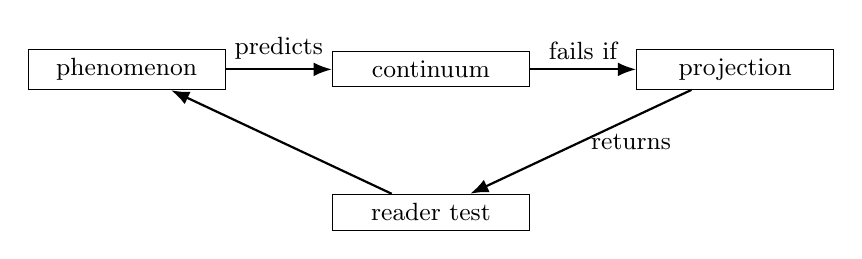
\begin{tikzpicture}[node distance=1.35cm,>=Latex,every node/.style={font=\small}]
\node[draw,align=center,minimum width=2.5cm] (c) {phenomenon};
\node[draw,align=center,minimum width=2.5cm,right=of c] (t) {continuum};
\node[draw,align=center,minimum width=2.5cm,right=of t] (f) {projection};
\node[draw,align=center,minimum width=2.5cm,below=of t] (r) {reader test};
\draw[->,thick] (c) -- node[above]{predicts} (t);
\draw[->,thick] (t) -- node[above]{fails if} (f);
\draw[->,thick] (f) -- node[right]{returns} (r);
\draw[->,thick] (r) -- (c);
\end{tikzpicture}
\caption{Physical Projection: falsifier of domain projection pressure 51-1-46}
\label{fig:figure-k0-physical-projection-one}
\end{figure}
The point of the diagram is not decoration; it marks which relation is being proposed and which stronger conclusion is still unavailable.\par
A local clarification is useful here\par
A local clarification is useful here\footnote{In Physical Projection, this note clarifies the reader clarification role of the term and keeps the caveat close to the sentence that needs it.}.\par
The note keeps the caveat near the term without derailing the main sentence.\par
The central phenomenon is the persistence of organized physical form under constraint. A form may be static, as in a crystal lattice; dynamic, as in a convection cell; reactive, as in an autocatalytic chemical set; or intermittent, as in a sandpile that alternates between quiet accumulation and sudden avalanche. OC calls the continuing field of possible states a continuum. In the physical projection, a continuum is not a mystical substrate. It is the range of materially possible configurations available to a system under specified conditions.\par
A boundary is the condition that separates one range of possible behavior from another. The wall of a container is a boundary, but so is a temperature threshold, a pressure regime, a concentration limit, a load capacity, a reaction condition, or an energy gradient. A boundary need not be a visible surface. It can be a limit in the behavior of the system. When water is heated from below, the transition from conductive heat transfer to organized convection is not caused by a newly visible wall. It appears when the previous mode can no longer carry the imposed gradient in the same way.\par
An operator is a repeatable action, relation, or transformation that changes the state of a system. In physical projection, an operator may be a flow, a collision, a reaction, a transport process, a dissipation channel, a constraint, or a mechanical action that selects which transformations are possible. The term does not add a hidden force. It gives a neutral name to what acts within the configuration. If nothing repeatable can be identified, the word operator has no useful work to do.\par
The difficulty is that physical science already has mature vocabularies. Entropy, energy, phase transition, symmetry breaking, reaction networks, attractors, stress, strain, and criticality all have technical meanings. OC cannot earn authority by renaming them. Its narrower use is comparative: it asks how different physical systems exhibit bounded persistence, transformation, unresolved constraint, new descriptive necessity, and loss of organization without pretending that one measurement scale fits all cases.\par
A shallow pan of fluid heated from below can carry the point from beginning to end. At low temperature difference, heat moves upward mainly by conduction. The fluid is materially active at microscopic scales, but its large-scale description remains smooth enough that no visible circulation pattern is needed. The continuum is the range of fluid states available under the pan, gravity, viscosity, thermal expansion, and imposed heating. The boundary is not only the pan wall; it is also the threshold at which conductive transport no longer remains the adequate macroscopic regime.\par
As the heat difference increases, small motions in the fluid can be amplified rather than damped. Above the relevant threshold, organized convection rolls may appear. The system has not gained purpose. It has reorganized because the prior mode no longer carries the imposed gradient under the same constraints. The operators include heat flow, buoyant motion, viscous damping, and circulation. The contradiction, in OC language, is the incompatibility between the imposed gradient and the continued adequacy of the old conductive organization. The emergence is not a miracle. It is the arrival of a new descriptive necessity: spatial circulation must now be named.\par
The same example also shows collapse. If the heating is changed, the geometry disturbed, or the fluid conditions altered, the convection pattern may weaken, fluctuate, reorganize, or disappear. Collapse does not mean matter vanishes. It means the named organization is no longer maintained. The pan still contains fluid. Heat still moves. But the particular bounded pattern that made convection rolls the right description has been lost. K0 is useful only when the configuration under discussion is named with that degree of care.\par
That account must remain modest. OC does not derive the equations of convection. It does not supply the critical Rayleigh number. It does not improve measurement. Its contribution is a higher-level description of why a new axis of description becomes relevant when an older description no longer carries the behavior. Work on self-organization in nonequilibrium systems is an appropriate scientific neighbor because it treats order as something that can arise in driven systems far from equilibrium, not as something imported from outside matter.\par
\section{Local Quantities In Physical Projection}
The projection map is the discipline that keeps OC vocabulary from drifting. Continuum maps to a physically constrained state space: the set of states a system can occupy under a specified material arrangement. Boundary maps to thresholds, interfaces, conservation limits, gradients, exclusion conditions, and regime-separating constraints. Operator maps to lawful transformations such as transport, reaction, dissipation, aggregation, fracture, circulation, and feedback. Contradiction maps to an incompatibility among constraints that cannot be resolved while preserving the current organization. Collapse maps to the loss of the configuration being described. \cite{nicolis_prigogine_selforg,kauffman_autocatalytic}\par
This map is intentionally sparse. It does not say that every physical process is a contradiction. It does not say that every instability is emergence. It does not say that a mathematical singularity, a phase transition, a chemical threshold, and a mechanical failure are identical. It says only that they can sometimes be compared at the level of constrained configuration: what was stable, what changed, which boundary was crossed, what new description became necessary, and what would count as failure of the named form.\par
The local dependency can now be written without changing the claim it supports.\par
\begin{equation}\label{eq:equation-k0-physical-projection-two}
\operatorname{metaTheoryDebt}_{12} = \tau_{\mathrm{repair}}=\inf\{t:C(t)<\theta\}
\end{equation}
The relation names a local dependency, variable dictionary, and proof/evidence role; it is not a claim-status upgrade.\par
The formula is a restraint on the prose. It names the dependency that the surrounding paragraph is allowed to use.\par
The comparison below gives physical projection a set of quantities that can be inspected instead of merely admired.\par
\begin{table}[htbp]
\centering\small
\caption{Physical Projection: observable quantities and counter-pressure 51-2-46}
\label{tab:table-k0-physical-projection-one}
\begin{tabular}{@{}llll@{}}
\toprule
Level & Axis pressure & Operator burden & Transition test \\
\midrule
physical projection boundary & 60 units & declared case & fixes what is compared \\
residual pressure & 0.49 & dimensionless & shows unresolved load \\
projection loss & 0.46 & bounded interval & marks lost structure \\
countercase set & 25 cases & review sample & keeps a falsifier visible \\
\bottomrule
\end{tabular}
\end{table}
The table should be read locally: it narrows the comparison without pretending that the wider theory has been settled by a single surface.\par
The phrase new dimension of description has a specific meaning. It does not mean a new physical dimension like length, width, or time. It means that an additional variable, relation, scale, pattern, or organizational feature becomes necessary for an adequate account. In the heated-fluid example, circulation pattern becomes relevant. In a reaction network, catalytic closure may become relevant. In a granular pile, avalanche distribution may become relevant. In a crystal, defect structure may become relevant. The projection is valid only if the new descriptive dimension can be named in ordinary scientific terms.\par
The heated-fluid example gives the cleanest full projection. The continuum is the range of possible fluid states under gravity, heating, viscosity, geometry, and boundary conditions. The boundary is the threshold between conductive and convective regimes. The operators are thermal transport, buoyant movement, viscous resistance, and the circulation that redistributes heat. The contradiction is not a logical statement hidden in matter; it is the physical incompatibility between the imposed gradient and continued organization as simple conduction. Emergence is the need to describe rolls, cells, or flow patterns. Collapse is the disappearance of that pattern as a maintained organization.\par
A chemical example shows the same language under different laws. Kauffman's work on autocatalytic sets, and later RAF network theory around reflexively autocatalytic and food-generated sets, gives cases in which molecules help produce molecules that in turn support production elsewhere in the network. OC does not turn these models into metaphysics. It treats them as cases in which a collection of reactions may become describable as a bounded organization because the network relation, not only the individual reaction, matters.\par
In that chemical case, the continuum is the range of possible reaction states supported by available molecules and conditions. The boundary includes the food set, reaction rules, catalysts, spatial or environmental limits, and constraints on what can be produced. Operators are reactions and catalytic effects. A contradiction may appear when the network cannot maintain closure under resource limits, dilution, inhibition, or missing catalysts. Collapse would be the disappearance of the organized reaction regime, not the destruction of matter itself.\par
A bridge gives a more ordinary mechanical example. A bridge is not only steel, concrete, bolts, cables, and deck surface. It is an organization of load paths, material tolerances, geometry, joints, foundations, and environmental exposure. Its continuum is the range of structural states compatible with remaining a bridge. Its boundaries include design load, fatigue limits, corrosion limits, thermal expansion ranges, and foundation stability. Its operators include traffic loading, wind, vibration, stress transfer, material fatigue, inspection, repair, and weathering.\par
If a bridge is loaded beyond its tolerances, the relevant contradiction is the incompatibility between imposed forces and the continued preservation of the structural organization. Sometimes the response is transformation inside the organization: elastic deformation, load redistribution, or repair. Sometimes a new descriptive dimension becomes necessary: fatigue cracking, resonance, buckling, or progressive failure may need to be tracked. Sometimes the bridge collapses as a bridge. The matter remains, but the organization that carried people or vehicles across a span has ceased to hold.\par
The map also prevents overreach. If a system is fully described by existing variables and no new relation becomes necessary, OC has no special work to do. If the proposed boundary cannot be identified, the projection is weak. If the proposed operator is merely decorative language, the projection is invalid. If collapse is declared without specifying which configuration is lost, the claim has not been stated sharply enough.\par
The physical projection therefore carries later claims only after three separations are clear. OC vocabulary is not a replacement for domain equations. OC terms must be anchored to observable, computable, or otherwise scientifically recognized features of the system. OC speaks at the level of organization and description, not at the level of final causes or hidden intentions in nature. This separation matters because broad systems language often becomes so elastic that it explains everything and tests nothing. K0 earns use by narrowing speech.\par
\section{A Projection Under Stress In Physical Projection}
No new equation is required for K0 Physical Projection here. That absence is not a weakness by itself. A projection layer can be preparatory: it can state how later formulas would have to attach to physical systems without pretending that a formal result has already been supplied. The discipline is to say exactly what would need mathematical specification before a claim becomes more than a conceptual comparison. \cite{nicolis_prigogine_selforg,kauffman_autocatalytic}\par
The minimal formal shape is a constrained state space with transformations. Let a physical system be described by possible states, constraints that restrict those states, and transformations that move the system from one state to another. This is not presented as a new physical law. It is a neutral template. Many sciences already use richer versions of this pattern, including dynamical systems, statistical mechanics, reaction network theory, continuum mechanics, and control theory.\par
The local dependency can now be written without changing the claim it supports.\par
\begin{equation}\label{eq:equation-k0-physical-projection-one}
\operatorname{civilizationScale}_{12} = \operatorname{loss}_{\phi}=1-\frac{|E_{\phi}\cap E_{\mathrm{domain}}|}{|E_{\mathrm{domain}}|}
\end{equation}
The relation names a local dependency, variable dictionary, and proof/evidence role; it is not a claim-status upgrade.\par
The formula is a restraint on the prose. It names the dependency that the surrounding paragraph is allowed to use.\par
The local dependency can now be written without changing the claim it supports.\par
\begin{equation}\label{eq:equation-k0-physical-projection-three}
\operatorname{reflexiveLoop}_{12} = I_{\mathrm{axis}}=\frac{\operatorname{Var}(x\mid a)}{\operatorname{Var}(x)}
\end{equation}
The relation names a local dependency, variable dictionary, and proof/evidence role; it is not a claim-status upgrade.\par
The formula is a restraint on the prose. It names the dependency that the surrounding paragraph is allowed to use.\par
A small numerical test keeps the abstraction honest at the scale of a single decision.\par
\paragraph{Numerical example.} For physical projection, take support=0.45, projection loss=0.11, and 2 open obligations. The bounded score is 0.113; the example gives the reader a numeric scale without pretending to be empirical proof.\par
The numbers are deliberately small; their value is pedagogical, not evidential, unless the chapter binds them to a dataset elsewhere.\par
Within that template, a boundary is a condition that changes the available states or transformations. A threshold temperature may permit a phase change. A concentration threshold may permit a reaction regime. A stress threshold may permit fracture. A connectivity threshold may permit network-level behavior. A geometric condition may permit or suppress a flow pattern. The exact mathematics differs by case. OC only requires that the boundary be identifiable in the domain's own terms.\par
A contradiction, in the K0 projection, is not a logical inconsistency inside nature. Matter does not assert propositions. The term means that the current configuration faces jointly imposed constraints that cannot all be satisfied while preserving the same organization. An overloaded bridge does not contain an argument. It contains forces, material limits, geometry, and failure modes. OC calls the unresolved incompatibility a contradiction only at the level of organized configuration.\par
The working hypothesis can now be read physically without inflation: when such an incompatibility remains unresolved, the system either requires a new descriptive dimension or loses the configuration under discussion. This is not a tested law of all physical systems. It is a proposed interpretive rule for examining bounded organization. The heated fluid may require pattern variables. The autocatalytic network may require closure variables. The sandpile may require avalanche statistics. The overloaded bridge may require fracture or fatigue variables, or it may simply fail as a bridge.\par
This is where scientific status discipline matters most. K0 Physical Projection does not prove the working hypothesis. It provides a vocabulary for asking whether the hypothesis can be made domain-specific. A rigorous physical claim would need a system definition, state variables, boundary conditions, transformation rules, and criteria for persistence, emergence, or collapse. Without those details, the claim remains preparatory and comparative.\par
The phrase formula surface names the place where prose touches possible mathematics. In this section, that contact is intentionally limited. It is enough to mark what a later equation, model, or simulation would have to do: define the relevant state space, specify operators, identify boundary conditions, distinguish transformation from collapse, and say what would count against the description. Anything stronger would give the present material more formal status than it has earned.\par
The heated-fluid example can be written against this surface without deriving the underlying equations. The system is a fluid layer under gravity, heated from below and cooled or bounded above. The continuum is the set of admissible velocity, temperature, and pressure fields under the material and geometric constraints. The boundary includes the threshold at which conduction loses stability as the adequate macroscopic regime. The operators are transport, buoyancy, viscosity, and heat exchange. The emergent descriptive dimension is patterned flow. Collapse is the loss of that organized flow regime.\par
The bridge example can also be written formally without pretending to solve engineering analysis. The system is a load-bearing structure with defined materials, geometry, supports, and use conditions. The continuum is the set of structural states compatible with continued function. Boundaries include load rating, yield points, fatigue thresholds, buckling limits, corrosion limits, and foundation constraints. Operators include applied loads, stress redistribution, material degradation, vibration, repair, and inspection. Collapse is not every crack or deformation. It is the loss of the named load-bearing organization.\par
A useful objection arises here. If every scientific model already defines variables and transformations, why add OC at all? The answer is that OC is not trying to outperform the local model. It is trying to compare the form of explanation across local models. A convection equation, a reaction network, a bridge analysis, and a sandpile model do not share the same observables, but each can be asked a common organizational question: which bounded configuration persists, which transformation becomes necessary, and which failure ends the configuration?\par
\section{Replay And Falsifier In Physical Projection}
Evidence surface names the limited contact zone between K0 language and established scientific evidence. It does not mean a new class of evidence, and it does not mean that OC is experimentally confirmed by borrowing results from other fields. It means the place where comparative OC claims must touch domain-specific work strongly enough to remain accountable. For K0, that evidence is indirect and comparative. It comes from literatures that show organized physical behavior arising under constraint, not from a dedicated OC experiment. \cite{nicolis_prigogine_selforg,kauffman_autocatalytic}\par
Work on self-organization in nonequilibrium systems provides one neighboring body of evidence. Autocatalytic-set research and later RAF network theory provide formal and conceptual cases where chemical organization depends on network relations. Work on self-organized criticality provides model families in which systems can approach states marked by scale-sensitive event patterns. These literatures do not certify OC. They supply disciplined examples that make the projection intelligible and also limit what OC may responsibly say.\par
The case that follows turns the proposal into a sequence of criticizable moves.\par
\paragraph{Worked case.} In the worked case for physical projection, the claim is reduced to a boundary, an observable, a dependency, a numerical cue, and a falsifier. The case is useful only because each move can be criticized separately.\par
The case helps because each step can fail separately, which is exactly what a useful example should permit.\par
A driven chemical system, a catalytic network, a critical sandpile, a convecting fluid, and an overloaded bridge each show that physical description often needs more than a list of components. Organization, threshold, relation, regime, and failure mode matter. OC uses those lessons as constraints on its own speech. When it talks about emergence, it must point to a change in descriptive necessity. When it talks about collapse, it must point to a lost organization. When it talks about boundary, it must name the condition doing the separating.\par
The evidence standard is modest. A citation can support the existence of a kind of physical phenomenon, such as nonequilibrium self-organization or autocatalytic closure. It cannot by itself support a sweeping claim about all systems. A comparison can show that OC vocabulary fits several examples. It cannot show that the vocabulary is complete. A conceptual map can prepare later scientific claims. It cannot replace measurement, derivation, simulation, independent replication, or the ordinary work by which scientific claims become reliable.\par
Return to the heated fluid. The physical evidence belongs to fluid dynamics and nonequilibrium physics: experiments, equations, stability analysis, dimensionless numbers, and observed pattern formation. OC adds no measurement to that literature. Its evidence-facing value is narrower. It asks whether the system can be described as a bounded configuration, whether a regime-separating boundary can be named, whether operators can be identified, whether a new descriptor becomes necessary after the threshold, and whether loss of the pattern can be distinguished from mere variation within it.\par
The same caution applies to autocatalytic networks. It is tempting to say that life itself has been explained once catalytic closure is described. That would be too strong. Autocatalytic and RAF models illuminate possible routes to chemical organization, but they do not settle all questions about the origin of life, biological evolution, or cellular complexity. OC may use them to clarify what it means for a new organizational level to become describable. It may not use them to claim more than those models establish.\par
Consider also the sandpile model associated with self-organized criticality. Grains are added slowly. For a time, the pile absorbs them through small adjustments. Eventually, some additions trigger avalanches of different sizes. The scientific literature around this model concerns critical states, scaling behavior, and dynamics under slow driving and relaxation. OC can describe the pile as a bounded configuration whose local additions create tensions that sometimes reorganize the whole. But the OC description is secondary. The scientific content remains in the model, its assumptions, its mathematics, and its empirical limits.\par
A physical projection can face readers honestly only when it keeps this humility. It may say: here is a family of phenomena in which organization appears under constraint. It may say: OC offers a shared vocabulary for describing boundary, operator, emergence, and collapse across those phenomena. It may not say: OC has proven the physics, solved the chemistry, replaced engineering, or reduced all material organization to one formula.\par
The evidence surface is strongest where OC forces more explicit questions. What is the system? What boundary defines it? What transformations preserve it? What transformations destroy it? What new variable becomes necessary after a threshold is crossed? What would show that no such new variable is needed? These questions are not evidence by themselves, but they make evidence easier to organize. They also make weak claims easier to reject.\par
The objection here is direct: a vocabulary that depends on other sciences may be parasitic. The answer is that every projection layer depends on the domain it projects into. K0 is not a rival laboratory. It is a comparative language. Its success depends on whether it helps physical claims become more exact, more bounded, and more rejectable than they were before.\par
\section{What Survives Translation In Physical Projection}
A physical projection must be able to fail. If it cannot fail, it is not disciplined language; it is ornament. K0 therefore needs rejection conditions as much as examples. Because this projection is not one grand equation, its failures are local. A K0 use fails when its terms cannot be anchored to the physical system being discussed, when they add no discriminating content, or when they misdescribe established science. \cite{nicolis_prigogine_selforg,kauffman_autocatalytic}\par
The most basic failure is empty mapping. If continuum, boundary, operator, contradiction, emergence, and collapse can be assigned arbitrarily to any feature of a system, the projection has lost its purpose. A term that can attach anywhere explains nothing. A valid K0 use must identify a real range of possible physical states, a boundary that separates regimes or constraints, and an operator that corresponds to a recognized transformation. In the heated-fluid case, these requirements are concrete: fluid states, thermal threshold, transport, buoyancy, viscosity, and circulation.\par
The next failure appears when emergence is announced without need. A system may change continuously while remaining adequately described by the same variables. A temperature value may rise. A pressure may fall. A load may increase. Not every numerical change opens a new descriptive dimension. If the supposed threshold is crossed and no new variable, relation, scale, pattern, or organizational descriptor becomes necessary, the OC claim has not been supported. Emergence requires a change in what must be described, not merely a change in magnitude.\par
Collapse also has to be protected from inflation. A system may fluctuate, deform, adapt, repair, transition, or reconfigure without losing the organization under discussion. A bridge that flexes under ordinary load has not collapsed. A convection roll that shifts position has not necessarily collapsed. A reaction network that changes rate has not necessarily lost its organizational regime. Collapse means the named configuration no longer holds. Without that named configuration, the word becomes theatrical rather than analytic.\par
Scientific vocabulary supplies another boundary for the projection. If OC prose contradicts established physical usage, the error belongs to OC. Entropy cannot be treated as a loose synonym for disorder whenever that is rhetorically convenient. Criticality cannot be invoked without attention to the model conditions under which the term has meaning. Autocatalysis cannot be used as a generic word for any self-reinforcing process. Stress, fracture, phase, equilibrium, and energy all carry local disciplines. K0 must speak through those disciplines, not over them.\par
There is also a failure of surplus metaphysics. A convection roll does not want to resolve contradiction. A reaction network does not seek closure. A sandpile does not decide to become critical. A bridge does not intend to remain a bridge. OC may describe organization, transformation, and loss of configuration; it may not smuggle agency, destiny, hidden purpose, or cosmic preference into matter. Physical projection stops where intention is added to systems that have not been shown to possess it.\par
A practical test is to rewrite any K0 claim in domain language. If the rewritten claim disappears, the OC version was probably decorative. If the rewritten claim becomes clearer, more limited, or more testable, the projection is doing work. For the heated-fluid case, the domain rewrite refers to thermal gradient, instability, convection, and pattern formation. The OC version is acceptable only if it helps compare that case with other boundary crossings without distorting the physics.\par
The bridge example makes the same test severe. To say that a bridge faces contradiction is too vague. To say that an imposed load, corrosion state, support condition, or vibration regime exceeds what the structure can accommodate while preserving its load-bearing organization is clearer. To say that the bridge collapses is too vague unless the lost organization is specified. Did a member yield? Did a joint fail? Did the span lose load path continuity? Did the structure cease to function as a bridge? K0 becomes useful only as the domain account becomes sharper.\par
These rejection conditions may make OC seem dependent on existing science. At the physical level, that dependence is not a defect. K0 is not claiming independence from physics, chemistry, materials science, or engineering. Its independence lies in the cross-domain form of questioning. It asks how bounded configurations become describable, transform, or fail. The physical answer must still come from the sciences that study the physical system directly.\par
\section{The Domain Enters In Physical Projection physicsS}
Current science already contains powerful accounts of the phenomena K0 touches. Nonequilibrium thermodynamics studies systems maintained away from equilibrium by flows of energy or matter. Nonlinear dynamics studies systems whose behavior cannot be understood by simple proportional response. Statistical mechanics connects microscopic states with macroscopic behavior. Reaction network theory studies how chemical reactions form structured systems. Materials science and engineering study stress, failure, fatigue, fracture, and the persistence of designed structures. The physics of critical phenomena studies transitions and scaling behavior near special regimes. \cite{nicolis_prigogine_selforg,kauffman_autocatalytic}\par
K0 Physical Projection sits beside these fields as an interpretive and comparative layer. Its first task is translation across examples. A convection roll, an autocatalytic network, a bridge, and a self-organized critical sandpile are not the same physical object. Yet all four involve bounded organization, constraints, transformations, and regime-sensitive description. OC gives names to those shared structural questions while leaving each domain's technical account intact.\par
The comparison with nonequilibrium self-organization is especially important because it makes order in driven systems scientifically ordinary rather than mysterious. Physical order can arise through lawful transformation under constraint. OC can borrow that lesson, but not its authority. The physical facts remain in the nonequilibrium models, experiments, and equations. OC merely says that such cases show why a theory of continua and boundaries must allow organization to appear without importing design from outside matter.\par
The comparison with Kauffman and RAF network theory clarifies relational organization. A chemical inventory may not be enough to describe a system if the reactions among components create closure properties. OC calls attention to the boundary between a list of reactions and a network-level regime. But the details belong to the chemical and mathematical models: which reactions exist, which catalysts are present, which food set is assumed, what closure condition is satisfied, and what breaks the organization.\par
The comparison with self-organized criticality clarifies the difference between ordinary accumulation and regime-level behavior. A sandpile is simple enough to be memorable, but the science is not the childhood image of a pile of sand. The relevant models concern slow driving, local thresholds, avalanches, and distributions of event sizes. OC may use the example to illustrate boundary, operator, and reconfiguration. It may not flatten the technical literature into a slogan.\par
The comparison with bridges and other engineered structures adds a useful restraint. Not every physical system becomes more interesting when redescribed in OC terms. Sometimes the best account is ordinary engineering analysis: loads, material properties, fatigue, buckling, corrosion, inspection, and repair. OC earns its place only when it clarifies the organization being preserved or lost. A bridge is a good reminder that collapse is not a mood or a metaphor. It is a failure of a specified load-bearing configuration.\par
Against current science, OC has three possible virtues and three obvious risks. The virtues are portability, vocabulary discipline, and rejection awareness. Portability means the same organizational questions can travel across domains. Vocabulary discipline means each term must be mapped before it is used. Rejection awareness means the projection contains conditions under which its own use fails. The risks are vagueness, overgeneralization, and scientific trespass. Vagueness appears when terms are not anchored. Overgeneralization appears when examples are treated as universal proof. Scientific trespass appears when OC speaks over the domain rather than through it.\par
The K0 projection can carry later scientific claims only if those risks remain controlled. Later claims may become mathematical, computational, or empirical, but this opening layer does not grant them that status in advance. It prepares the grammar of the claim. A later study would still need its own model, data, implementation, comparator, uncertainty analysis, and rejection conditions.\par
The handoff is therefore precise. K0 gives the physical meaning of OC's basic terms: continuum as constrained possibility, boundary as regime-separating condition, operator as transformation, contradiction as unresolved constraint incompatibility, emergence as new descriptive necessity, and collapse as loss of the named organization. With those meanings in place, later parts of the monograph can ask whether the same structure projects into biological, cognitive, social, or formal domains without pretending that those domains share the same measurements.\par
\chapter{K1 Chemical Projection}
\section{The Domain Enters In Chemical Projection}
Chemistry occupies the difficult middle ground between inert arrangement and living maintenance. A salt crystal preserves order, but it does not repair the conditions of its own formation. A flame continues only while fuel and oxygen pass through it. A polymer gel can swell, contract, and hold a history of preparation in its structure. A catalytic cycle can return to an earlier state while converting material around it. A prebiotic pool, if it is not merely a pool of debris, must do something still more demanding: it must let some transformations recur while others disappear. This is the region in which matter begins to display persistence without yet becoming life. \cite{kauffman_autocatalytic,raf_networks}\par
The chapter title, K1 Chemical Projection, names the first chemical use of the book's general vocabulary. The name should not be allowed to obscure the ordinary phenomenon. K1 is simply the chemical case: the place where molecules, reactions, energy flow, concentration, surfaces, and compartments are considered together because none of them alone is the whole event. A molecule can be present and still be irrelevant to the continuing pattern. A reaction can occur once and leave no organized consequence. A catalyst can accelerate a step without governing a system. What matters here is the patterned continuation of transformations under conditions that permit some chemical futures and prevent others.\par
The next diagram slows the argument down just enough to show how chemical projection is being organized.\par
\begin{figure}[htbp]
\centering
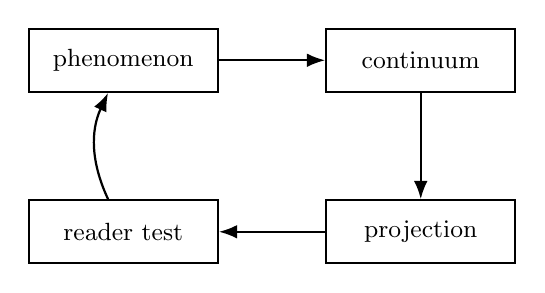
\begin{tikzpicture}[node distance=1.35cm,>=Latex,every node/.style={font=\small}]
\node[draw,thick,align=center,minimum width=2.4cm,minimum height=0.8cm] (a) {phenomenon};
\node[draw,thick,align=center,minimum width=2.4cm,minimum height=0.8cm,right=of a] (b) {continuum};
\node[draw,thick,align=center,minimum width=2.4cm,minimum height=0.8cm,below=of b] (c) {projection};
\node[draw,thick,align=center,minimum width=2.4cm,minimum height=0.8cm,left=of c] (d) {reader test};
\draw[->,thick] (a) -- (b);
\draw[->,thick] (b) -- (c);
\draw[->,thick] (c) -- (d);
\draw[->,thick,bend left=25] (d) to (a);
\end{tikzpicture}
\caption{Chemical Projection: state transition of domain projection pressure 52-1-47}
\label{fig:figure-k1-chemical-projection-one}
\end{figure}
The point of the diagram is not decoration; it marks which relation is being proposed and which stronger conclusion is still unavailable.\par
A local clarification is useful here\par
A local clarification is useful here\footnote{In Chemical Projection, this note clarifies the reader clarification role of the term and keeps the caveat close to the sentence that needs it.}.\par
The note keeps the caveat near the term without derailing the main sentence.\par
The book calls its larger framework OC. At this point the initials need only carry a modest meaning. OC asks how an organized field of possibilities changes when its own continuation becomes strained. In chemistry, that field is not mystical or detached from matter. It consists of actual species, possible reactions, concentrations, energetic gradients, catalytic relations, phase behavior, surfaces, compartments, and timescales. When such a field is sustained long enough to have a recognizable range of possible next states, this chapter will call it a continuum. The term does not replace solution chemistry, kinetics, thermodynamics, or molecular mechanism. It gives a name to the whole condition-space in which chemical change is taking place.\par
A boundary is then any condition that separates transformations that can continue from transformations that cannot. Some boundaries are visible: a vesicle wall, a mineral pore, an oil-water interface, the wall of a reactor. Others are less pictorial but no less real: a pH range, a temperature window, a redox condition, a drying cycle, a limited feedstock, a diffusion length, an activation barrier. Chemistry is unforgiving about such boundaries. The same written equation can behave differently when the solvent changes, when the concentration falls below a threshold, when a surface adsorbs an intermediate, or when heat destroys the molecule that a reaction was supposed to accumulate.\par
Within that bounded continuum, a reaction becomes important when it does more than occur. It may change what can happen next. It may replenish a scarce intermediate, remove an inhibitor, open a pathway, close a pathway, concentrate a product, or produce a catalyst for a later step. In the language of this book, such a repeatable transformation is an operator. The word is not a new chemical mechanism. It is a role-name. A bond rearrangement remains a bond rearrangement; catalysis remains catalysis; diffusion remains diffusion. But when any of these transformations alters the continuing organization of the chemical field, it is useful to name the role it plays.\par
The last term needed before the examples is contradiction. In ordinary speech, contradiction sounds like a clash between propositions. In chemistry, the relevant clash is material. A network may require concentration for productive encounters while dilution constantly disperses its members. It may require energy throughput while too much energy destroys intermediates. A compartment may protect products while blocking feedstock. A mineral surface may stabilize one molecule while trapping another so strongly that the next reaction cannot proceed. These are not metaphors for disagreement. They are incompatibilities in continuation. The system cannot keep going in the same way unless the incompatibility is resolved, displaced, buffered, or endured until collapse.\par
Emergence enters only after this pressure is visible. A chemical pattern is emergent in the limited sense used here when the significant property belongs to an organization of transformations rather than to an isolated molecule or isolated reaction. A single molecule does not contain an autocatalytic set. A single equation does not contain persistence under changing feed. A list of products does not by itself contain a system. The higher-level description earns its place only when it identifies something real about the continuing organization that would be missed by treating every reaction as an independent event.\par
\section{Local Quantities In Chemical Projection}
Begin with a small imagined cycle, because it exposes the issue cleanly. Molecule A helps produce molecule B, B helps produce molecule C, and C helps regenerate A. No member of the trio is the whole phenomenon. If A is present once and then disappears, there is no continuing organization. If B forms but cannot reach the reaction that makes C, the written cycle is only a diagram. If C regenerates A too slowly, side reactions may drain the system before closure matters. If feedstock enters at the right rate and waste leaves without destroying the needed intermediates, the same pattern may persist for many turns. The interesting object is not A, B, or C, but the relation among their transformations under the conditions that allow recurrence. \cite{kauffman_autocatalytic,raf_networks}\par
This is why chemical organization cannot be read directly from a formula sheet. Formulae are indispensable, but they are compressed descriptions. They do not by themselves specify whether a reaction is fast enough, whether an intermediate survives long enough, whether a catalyst is poisoned, whether the solvent changes the pathway, whether a surface concentrates one species and excludes another, or whether the products accumulate until the system blocks itself. A drawn network can be true as a possibility and false as an account of behavior. Chemistry lives in that gap between possible connection and actual continuation.\par
The local dependency can now be written without changing the claim it supports.\par
\begin{equation}\label{eq:equation-k1-chemical-projection-two}
\operatorname{historicalInheritance}_{12} = \rho_{\mathrm{replay}}=\frac{N_{\mathrm{matched}}}{N_{\mathrm{declared}}}
\end{equation}
The relation names a local dependency, variable dictionary, and proof/evidence role; it is not a claim-status upgrade.\par
The formula is a restraint on the prose. It names the dependency that the surrounding paragraph is allowed to use.\par
The comparison below gives chemical projection a set of quantities that can be inspected instead of merely admired.\par
\begin{table}[htbp]
\centering\small
\caption{Chemical Projection: observable quantities and counter-pressure 52-2-47}
\label{tab:table-k1-chemical-projection-one}
\begin{tabular}{@{}llll@{}}
\toprule
Example & Parameter & Value & What changes \\
\midrule
chemical projection boundary & 63 units & declared case & fixes what is compared \\
residual pressure & 0.56 & dimensionless & shows unresolved load \\
projection loss & 0.57 & bounded interval & marks lost structure \\
countercase set & 26 cases & review sample & keeps a falsifier visible \\
\bottomrule
\end{tabular}
\end{table}
The table should be read locally: it narrows the comparison without pretending that the wider theory has been settled by a single surface.\par
Network thinking is still valuable. It lets us stop pretending that every molecule can be understood in isolation. A reaction network can show which species feed which pathways, where catalysts enter, where loops appear, and where a small loss may break a larger pattern. Systems chemistry has made this kind of thinking central by studying how interacting chemical components generate collective behavior: oscillation, replication-like amplification, self-sorting, compartmentalization, adaptive response, or pathway selection. Origin-of-life research asks a sharper historical question: how nonliving chemistry could have generated organizations capable of maintenance, reproduction, and eventually evolvability. Chemical reaction network theory supplies formal tools for analyzing reaction systems. Philosophical ontology asks what kind of thing a continuing organization is. These disciplines overlap, but they do not ask the same question.\par
OC enters after those distinctions are respected. It does not claim that chemistry lacks its own concepts. Chemistry has stronger tools than any general vocabulary can replace: kinetics, thermodynamics, statistical mechanics, catalysis, spectroscopy, chromatography, reactor design, surface science, and molecular simulation. The value of K1 is narrower. It asks how to speak about the level at which a chemical organization persists, strains, reorganizes, or fails without pretending that this level is either a single molecule or a free-floating abstraction.\par
The word projection matters in that narrow sense. A projection is a translation into a domain that remains answerable to that domain. When the book speaks of a chemical continuum, it must be able to point to species, reactions, concentrations, energy sources, compartments, and timescales. When it speaks of a boundary, it must be able to say what condition permits or prevents continuation. When it calls a transformation an operator, it must identify the chemical process and the role it plays. When it speaks of contradiction, it must name the material incompatibility. When it speaks of emergence, it must show why a system-level description captures something that isolated reactions do not.\par
This discipline becomes clearer in autocatalytic organization. Stuart Kauffman made autocatalytic sets prominent in origin-of-life theory by arguing that sufficiently rich chemical repertoires may contain subsets whose members collectively support one another's production. Later work on RAF networks, short for reflexively autocatalytic and food-generated networks, gave the idea more explicit conditions. A RAF set requires reactions catalyzed by members of the system and reactants that can be built from an allowed food set. That definition does not prove how life began, and it does not turn every complex mixture into an organized system. It does something more useful for this chapter: it shows how a collective chemical object can be defined with more rigor than loose talk of complexity.\par
The important lesson is not that all chemical emergence must be RAF-like. It is that chemical closure can be stronger than metaphor. A network may be organized not because it looks tangled, but because its members help regenerate the very conditions under which the network continues. At that point the reader has reason to describe a higher-level pattern. The claim is still chemical. It remains vulnerable to rates, yields, poisoning, dilution, heat, solvent, side reactions, and the availability of feedstock. But it is no longer adequately described as a mere heap of independent reactions.\par
\section{A Projection Under Stress In Chemical Projection}
A richer example can be taken from one of the classic reactions in prebiotic chemistry: the formose reaction. In its simplest description, formaldehyde in alkaline aqueous solution can produce sugars. The reaction was discovered in the nineteenth century, and it has never stopped being both attractive and troublesome. It is attractive because formaldehyde is a small molecule, because sugars are central to biochemistry, and because the reaction contains autocatalytic features. It is troublesome because it is messy, condition-sensitive, and prone to producing complex mixtures rather than a clean path toward biological order. \cite{kauffman_autocatalytic,raf_networks}\par
The usual starting point is formaldehyde, often under basic conditions, with calcium hydroxide or other alkaline catalysts appearing in many versions. Two molecules of formaldehyde can combine through early steps to form glycolaldehyde. Once glycolaldehyde is present, it can participate in pathways that accelerate further sugar formation. The reaction may show an induction period followed by more rapid product formation, a behavior that has often been associated with autocatalysis. Products can include a range of sugars and related compounds, not a single chosen molecule marching toward life. Under many conditions the mixture continues onward into degradation, side products, and tar-like complexity.\par
The local dependency can now be written without changing the claim it supports.\par
\begin{equation}\label{eq:equation-k1-chemical-projection-one}
\operatorname{grandSynthesis}_{12} = G=(V_{\mathrm{claim}}\cup V_{\mathrm{evidence}},E_{\mathrm{support}}\cup E_{\mathrm{challenge}})
\end{equation}
The relation names a local dependency, variable dictionary, and proof/evidence role; it is not a claim-status upgrade.\par
The formula is a restraint on the prose. It names the dependency that the surrounding paragraph is allowed to use.\par
The local dependency can now be written without changing the claim it supports.\par
\begin{equation}\label{eq:equation-k1-chemical-projection-three}
\operatorname{methodFalsifier}_{12} = \epsilon_{\mathrm{domain}}=\max_i |y_i-\hat y_i|
\end{equation}
The relation names a local dependency, variable dictionary, and proof/evidence role; it is not a claim-status upgrade.\par
The formula is a restraint on the prose. It names the dependency that the surrounding paragraph is allowed to use.\par
A small numerical test keeps the abstraction honest at the scale of a single decision.\par
\paragraph{Numerical example.} For chemical projection, take support=0.48, projection loss=0.16, and 3 open obligations. The bounded score is 0.; the example gives the reader a numeric scale without pretending to be empirical proof.\par
The numbers are deliberately small; their value is pedagogical, not evidential, unless the chapter binds them to a dataset elsewhere.\par
This example is useful because it refuses romance. The formose reaction gives a plausible chemical route from a simple carbon source to biologically interesting molecules, but it also displays the severe selectivity problem that origin-of-life chemistry must face. A reaction that makes everything a little can fail to make anything in a sustained, useful way. If ribose appears only in small amounts and rapidly degrades, its momentary presence is not yet an explanation for RNA-world chemistry. If alkaline conditions promote sugar formation but also destruction, the same boundary that enables the pathway may undermine its accumulation. If calcium helps organize certain intermediates, it may also favor pathways that do not lead where a later story wants to go.\par
In K1 language, the continuum includes formaldehyde, early sugar intermediates such as glycolaldehyde, catalytic bases or metal ions, water, pH, temperature, concentration, side reactions, and the timescale over which products form and decay. The boundary is not only the beaker wall. It is the alkaline range in which the relevant carbon-carbon bond-forming chemistry becomes possible; the concentration regime in which reactive intermediates meet; the thermal range in which products survive long enough to matter; and any mineral, borate, phosphate, or compartmental condition that stabilizes some molecules while suppressing others. The operators are the repeatable transformations: aldol additions, isomerizations, retro-aldol cleavages, catalytic steps, precipitation or adsorption events, dilution, drying, rehydration, and degradation.\par
The contradiction is immediate. The system needs reactivity, but reactivity threatens selectivity. It needs alkaline activation, but alkaline solution can also destroy fragile sugars. It needs concentration, but concentration can accelerate both desired pathways and destructive side reactions. It needs a supply of formaldehyde, but uncontrolled supply can drive unselective complexity. The formose reaction is therefore not merely an example of chemical creativity. It is an example of chemical pressure: the very conditions that open the continuum also generate paths by which the continuum loses the organization one might hope to see.\par
What is known here belongs to ordinary chemistry. Formaldehyde can undergo base-catalyzed carbon-carbon bond formation. Glycolaldehyde can accelerate further sugar production. Product distributions depend strongly on conditions. Additives and surfaces can alter selectivity and stability. Analytical chemistry can detect products, follow concentration changes, and compare reaction conditions. None of that requires OC. It is the chemical ground on which any higher description must stand.\par
What is modeled belongs to several levels. A reaction scheme can represent the possible transformations among formaldehyde, glycolaldehyde, higher sugars, and degradation products. A kinetic model can assign rate constants and simulate concentration over time. A network representation can show loops, drains, hubs, and possible autocatalytic relations. A geochemical scenario can place the reaction in a drying pond, mineral pore, alkaline vent, evaporating film, or ice-brine pocket. Each model answers a different question. A network diagram may identify possible closure while remaining silent about whether the rates are plausible. A kinetic simulation may show persistence under selected parameters while remaining silent about whether those parameters existed on early Earth. A laboratory experiment may show product formation while remaining silent about geological frequency.\par
What remains speculative is the historical and organizational leap. Did formose-like chemistry occur in relevant prebiotic environments? Did it persist long enough, and with enough selectivity, to feed later chemistry? Did mineral surfaces, borate stabilization, compartmental cycling, or environmental rhythms solve enough of the selectivity problem to matter? Did sugar formation couple to other reaction systems rather than remain an isolated burst of products? These questions cannot be answered by the existence of the reaction alone. They require evidence about conditions, coupling, persistence, and downstream consequence.\par
OC is allowed to add only a description of organization under strain. It may say that the formose reaction displays a continuum rich enough to generate many possible transformations. It may identify boundaries that enable and constrain those transformations. It may describe the autocatalytic acceleration associated with glycolaldehyde as an operator relation within the system. It may name the contradiction between productive reactivity and destructive loss. It may ask whether any environmental or chemical arrangement reorganizes the system so that persistence becomes possible: for example, by stabilizing certain sugars, periodically refreshing feedstock, separating products, adsorbing inhibitors, or coupling sugar formation to a larger network.\par
It may not say that the formose reaction proves the origin of life. It may not treat a diagram of autocatalysis as a laboratory result. It may not treat a laboratory result as a geological history. It may not treat a geological possibility as evidence of a universal principle. The value of the example is precisely that it keeps all those layers visible. A reaction can be real, a model can be instructive, a scenario can be plausible, and the larger claim can still remain unproven.\par
The example also clarifies the phrase that matter can remember constraints. In chemistry this should be heard physically, not psychologically. A polymer can preserve a sequence or cross-linked structure. A mineral surface can template adsorption. A gel can retain a pattern of swelling, charge, or trapped solute. A reaction network can display hysteresis, so that its later behavior depends on its earlier path. A concentration cycle can leave products that alter the next cycle. A kinetically trapped state can persist after the conditions that formed it have changed. Chemical memory means persistence, stored structure, path dependence, templating, or delayed release of constraint into later behavior. It is not intention and not biological heredity unless further machinery is present.\par
\section{Case And Countercase In Chemical Projection}
The formose reaction shows why emergence must be used sparingly. It is tempting to see any autocatalytic acceleration as a new level of organization. That temptation should be resisted. If the only claim is that glycolaldehyde accelerates further production under alkaline conditions, ordinary chemical kinetics may be enough. The higher-level description becomes useful only when the pattern of transformations has a property that belongs to the organized set: persistence across cycles, regeneration of enabling intermediates, selective stabilization, coupling to feedstock, or a transition between regimes that cannot be understood by naming one reaction in isolation. \cite{kauffman_autocatalytic,raf_networks}\par
RAF theory helps here because it formalizes one kind of closure. In a RAF network, every reaction is catalyzed by something produced within the system or available from the food set, and every reactant can be generated from that food set. This is a stricter idea than saying that a mixture is complicated. It asks whether the network collectively supports its own reactions from allowed inputs. If a candidate network fails those conditions, the story must change. Perhaps it is not closed. Perhaps it requires an external catalyst. Perhaps it is only a transient cascade. Perhaps the relevant organization lies elsewhere.\par
The case that follows turns the proposal into a sequence of criticizable moves.\par
\paragraph{Worked case.} In the worked case for chemical projection, the claim is reduced to a boundary, an observable, a dependency, a numerical cue, and a falsifier. The case is useful only because each move can be criticized separately.\par
The case helps because each step can fail separately, which is exactly what a useful example should permit.\par
A chemical graph is therefore both illuminating and dangerous. It can show that A connects to B, that B connects to C, and that C returns to A. It can reveal a loop that no single reaction equation makes obvious. But topology alone is not chemistry. Two networks with similar connectivity can behave differently if one has favorable kinetics and the other is blocked by activation barriers; if one intermediate survives minutes and the other survives microseconds; if one solvent stabilizes the transition state and another destroys the product; if one surface concentrates reactants and another poisons the catalyst. A graph is a claim about relation. Continuation requires kinetics, thermodynamics, transport, and environment.\par
Network science, in the broad tradition associated with work such as Newman's, supplies a mature language for paths, components, hubs, robustness, and connectivity. Those concepts can sharpen chemical thinking, especially when many species and reactions are involved. But chemical networks are not social networks with molecular labels attached. Edges are not all equal. Direction matters. Stoichiometry matters. Energetic feasibility matters. Rate laws matter. Spatial organization matters. A species with many connections may be central in a graph and chemically irrelevant if its reactions are too slow or its concentration too low. A small side path may dominate if it drains an essential intermediate.\par
Self-organized criticality enters only as a distant cousin, not as a master key. Some driven systems approach threshold regimes in which small events can be linked to large rearrangements. Chemistry certainly has thresholds: ignition, precipitation, gelation, phase separation, runaway reaction, catalyst poisoning, oscillatory transitions, and sudden loss of selectivity. But these are not all the same phenomenon. The useful point is modest: chemical systems under steady drive can cross boundaries where gradual change produces abrupt reorganization. The explanation must come from the specific chemistry, not from borrowing the prestige of a general threshold metaphor.\par
The same restraint applies to collapse. Many reaction systems do not reorganize into a higher order; they simply run down. Feedstock is exhausted. Intermediates hydrolyze. Catalysts are poisoned. Products inhibit further reaction. Compartments leak. Side reactions outcompete the pathway of interest. Heat denatures an organized structure. Dilution breaks the encounters on which recurrence depends. Collapse is not a disappointing exception to emergence. It is one of the main outcomes that makes emergence meaningful when it occurs.\par
This is why boundary conditions are not decorative details. A vesicle that preserves products but admits no new feedstock may turn persistence into starvation. A pore that concentrates reactants during drying may also trap products away from later reaction. A temperature cycle may open a pathway during heating and destroy its products before cooling. A pH shift may release a molecule from a surface while disabling the catalyst that made it. The boundary is not a passive frame around the real chemistry. It is part of the chemistry's possibility structure.\par
In this sense, chemical contradiction is not an exotic addition to scientific explanation. It is a way of pointing to the place where continuation becomes materially difficult. A system can respond by buffering the incompatibility, as when a compartment moderates dilution. It can displace it, as when a side pathway removes an inhibitor but creates a new dependency. It can reorganize, as when a set of reactions becomes coupled to a cycling environment that periodically restores needed conditions. It can also fail. The word contradiction names the pressure point, not the solution.\par
\section{What Survives Translation In Chemical Projection}
K1 sits beside current science, not above it. Systems chemistry studies how interacting components produce collective function. Origin-of-life research studies how nonliving chemistry might have generated self-maintaining and eventually evolvable systems. Chemical reaction network theory studies the formal behavior of reaction systems. Network science studies connected structure across many domains. Thermodynamics and kinetics remain the laws and measures without which no chemical claim can stand. OC does not outrank any of these fields. It asks a cross-level question that often appears between them: when does a chemical situation become intelligible as a continuing organization rather than as a list of parts? \cite{kauffman_autocatalytic,raf_networks}\par
The answer cannot be given by enthusiasm for complexity. A crowded mixture is not necessarily organized. A long reaction list is not necessarily a system. A loop in a diagram is not necessarily closure. A transient burst of product is not necessarily persistence. A resemblance to biology is not biology. The chemical standard remains hard: the relevant species must exist; the reactions must be feasible; the rates and yields must matter on the timescale claimed; the energetic and environmental conditions must be specified; the organization must survive comparison with simpler explanations.\par
At the same time, reduction to isolated steps can miss something real. A catalytic cycle is not understood by naming only one step if the cycle's importance lies in return. An oscillating reaction is not understood by listing products if the phenomenon is temporal pattern. A compartmentalized system is not understood by bulk concentration alone if spatial separation controls which reactions meet. A polymerization process is not understood by monomer chemistry alone if sequence, folding, templating, or kinetic trapping alters future possibilities. Chemistry repeatedly produces cases in which the organization of transformations is itself the object of explanation.\par
The useful distinction is between occurrence, persistence, regeneration, and reorganization. Occurrence means that a reaction happens. Persistence means that a pattern of transformations continues across time or cycles. Regeneration means that the system helps reproduce components or conditions needed for its own continuation. Reorganization means that under strain the system changes the level or form of its organization: a new compartment relation, a new catalytic loop, a new stabilized pathway, a new phase, a new coupling to an environmental cycle. These are not interchangeable claims. Confusing them is one of the easiest ways to make chemistry sound more alive, more settled, or more philosophically obedient than it is.\par
The formose reaction again supplies the caution. Formaldehyde conversion is occurrence. Repeated sugar production under maintained conditions may be persistence. Autocatalytic acceleration through glycolaldehyde is a step toward regeneration, but only within a constrained sense. Stabilization of selected products through borate, mineral surfaces, compartmental cycling, or coupling to another network would be a candidate for reorganization if it changes what can continue. None of these statements requires saying that life has begun. Each statement occupies a different level of chemical organization.\par
Current science also resists the fantasy of a single clean ladder. Chemical systems are noisy, leaky, parasitic, and historically contingent. A pathway that looks promising in a purified experiment may fail in a mixed environment. A catalyst that works in one solvent may be poisoned in another. A mineral surface may help at one concentration and hinder at another. A compartment may protect fragile molecules while excluding the feedstock needed to make them. A model may identify a possible network that no plausible prebiotic setting could maintain. These resistances are not obstacles to serious theory; they are what serious theory must absorb.\par
This is the reason for keeping analogy, formal model, simulation, experiment, and historical claim distinct. An analogy may guide attention. A formal model may clarify necessary conditions. A simulation may explore ranges of behavior. An experiment may show what happens under specified conditions. A historical claim must connect such results to environments that actually existed or plausibly existed. The layers can support one another, but they do not automatically convert into one another. A simulation of a self-sustaining network does not become a prebiotic event by being elegant. A laboratory reaction does not become a universal principle by being suggestive.\par
When K1 is used well, it sharpens rather than softens these distinctions. It asks what the continuum contains, where the boundaries lie, which transformations alter the system's future, what incompatibility threatens continuation, and whether any higher-level organization is actually needed to describe the result. If ordinary kinetics gives the full explanation at the right level, no additional emergence should be claimed. If a system-level property remains after the chemistry is specified, then the higher description has work to do.\par
\section{The Domain Enters In Chemical Projection chemistr}
The chemical projection is therefore a disciplined act of attention. It asks the reader to look neither below the phenomenon, where only isolated molecules appear, nor above it, where vague talk of life, order, or complexity floats free of chemistry. It holds the middle scale: the scale at which reactions compose networks, networks depend on boundaries, boundaries create pressures, pressures produce persistence or failure, and occasional reorganizations justify a new descriptive level. \cite{kauffman_autocatalytic,raf_networks}\par
The central claim is modest but important. Chemistry provides real cases in which matter does more than sit in arrangement and less than live. It can store structure, display path dependence, amplify intermediates, fall into cycles, exhaust itself, reorganize under changing conditions, and preserve traces of prior constraint in later behavior. These phenomena do not prove a general ontology. They make a general ontology answerable to matter. Any vocabulary that cannot survive contact with concentration, pH, temperature, solvent, rate, yield, and degradation has no right to speak for chemistry.\par
K1 earns its place only by remaining exposed to that contact. If calling a reaction an operator adds nothing beyond a new label, the term should be dropped. If calling a condition a boundary hides the actual pH, membrane, pore, surface, or energy threshold, the description has become vague. If calling a tension a contradiction replaces the chemical incompatibility rather than naming it, the word has failed. If emergence is claimed where a list of independent reactions gives the better account, the claim is inflated. The vocabulary is useful only when it lets a complex chemical organization be described more exactly than before.\par
The strongest objection remains the simplest one: chemistry already has its own explanations. That objection is correct, and the chapter depends on it. K1 is not a rival to chemical science. It is a way of carrying a cross-domain argument through chemistry without making chemistry symbolic. The projection is successful only when the chemical facts become more visible: the feedstock, the intermediates, the catalysts, the drains, the surfaces, the compartments, the cycles, the thresholds, the collapses. If those facts fade, the projection has turned into decoration.\par
The chapter can now leave the reader with a chemical intuition rather than a set of checks. A molecule matters when it changes what can happen next. A reaction matters when it participates in a continuing organization. A boundary matters when it selects among possible continuations. A contradiction matters when the system cannot preserve its form without confronting an incompatibility in its own conditions. Emergence matters only when the organization of transformations becomes the right level of description. Collapse matters because most chemical possibilities do not become persistent worlds.\par
This is the chemical lesson that K1 contributes to the larger argument. Between stone and cell lies a domain of constrained transformation. It is not alive, but it is not inert in the simple sense. It can accumulate history, lose history, amplify accidents, suppress possibilities, and sometimes form patterns that outlast the molecular events that compose them. To speak of such patterns responsibly, one must keep the molecule in view and still see beyond the molecule. That is the work of chemical projection.\par
\chapter{K2 Biological Projection}
\section{The Domain Enters In Biological Projection}
Biology is the domain in which a fixed description most quickly becomes inadequate. A living system is made of parts, but it is not exhausted by an inventory of them. A cell includes membranes, enzymes, gradients, genomes, signals, wastes, and repair processes. A tissue includes cells, vessels, extracellular matrix, immune traffic, mechanical load, and histories of injury. An organism includes tissues, but also circulating constraints: temperature, hormones, posture, hunger, infection, sleep, stress, and development. The biological object is therefore not a single thing waiting to be named once and for all. It is a maintained pattern, and its maintenance depends on distinctions that must be stable enough to preserve identity and permeable enough to exchange matter, energy, and information. \cite{raf_networks,bak_soc}\par
This chapter uses the vocabulary of OC, the Ontological Calculus, only in that limited sense: as a way of describing organized change without pretending that the ordinary sciences of life have been replaced. A continuum is a trackable range of variation: temperature, concentration, stiffness, immune activation, developmental state, oxygen tension, or population density. A boundary is a distinction that lets one treat something as this rather than that: cell from environment, self from non-self, viable tissue from necrotic tissue, organism from population. An operator is a repeatable transformation: catalysis, signaling, division, migration, selection, apoptosis, repair. These words are broad, but they earn their place only when they can be tied to observable biological variables.\par
The next diagram slows the argument down just enough to show how biological projection is being organized.\par
\begin{figure}[htbp]
\centering
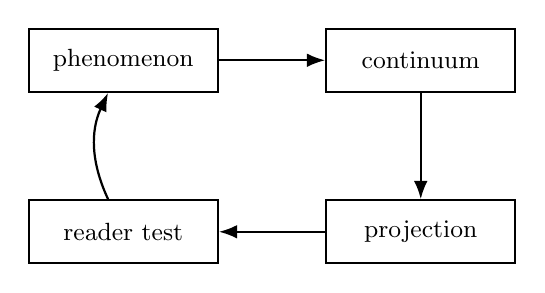
\begin{tikzpicture}[node distance=1.35cm,>=Latex,every node/.style={font=\small}]
\node[draw,thick,align=center,minimum width=2.4cm,minimum height=0.8cm] (a) {phenomenon};
\node[draw,thick,align=center,minimum width=2.4cm,minimum height=0.8cm,right=of a] (b) {continuum};
\node[draw,thick,align=center,minimum width=2.4cm,minimum height=0.8cm,below=of b] (c) {projection};
\node[draw,thick,align=center,minimum width=2.4cm,minimum height=0.8cm,left=of c] (d) {reader test};
\draw[->,thick] (a) -- (b);
\draw[->,thick] (b) -- (c);
\draw[->,thick] (c) -- (d);
\draw[->,thick,bend left=25] (d) to (a);
\end{tikzpicture}
\caption{Biological Projection: residual plot of domain projection pressure 53-1-48}
\label{fig:figure-k2-biological-projection-one}
\end{figure}
The point of the diagram is not decoration; it marks which relation is being proposed and which stronger conclusion is still unavailable.\par
A local clarification is useful here\par
A local clarification is useful here\footnote{In Biological Projection, this note clarifies the reader clarification role of the term and keeps the caveat close to the sentence that needs it.}.\par
The note keeps the caveat near the term without derailing the main sentence.\par
A simple wound shows why such language can be useful. Skin is cut. Blood vessels rupture. Platelets adhere to exposed matrix, fibrin begins to form, and a clot establishes temporary closure. Damaged cells release signals. Neutrophils arrive first, then macrophages, and the local chemistry changes as oxygen availability, cytokine concentration, microbial burden, pH, and protease activity shift. Fibroblasts later enter the region, endothelial cells support new vessels, keratinocytes migrate from the edge, and collagen is deposited, reorganized, and eventually remodeled. Nothing here is mysterious in the ordinary biological sense. The point is different: as the event unfolds, the relevant object changes. At one moment the useful object is a torn vessel wall; then a clot; then a chemical gradient; then an immune field; then a migrating epithelial sheet; then a collagen scaffold; then a scar or a restored surface.\par
That shifting object is not arbitrary. It is constrained by diffusion, blood flow, cell adhesion, receptor binding, mechanical tension, matrix stiffness, infection pressure, and the metabolic state of the tissue. A surgeon, immunologist, developmental biologist, and materials scientist may each notice a different boundary in the same wound. The wound edge is visible. The inflammatory boundary is chemical and cellular. The mechanical boundary appears in tissue tension. The microbial boundary depends on colonization, immune recognition, and antibiotic penetration. The organismal boundary appears when local injury threatens fever, sepsis, pain, mobility, or survival. Biology forces description to move, but it does not permit description to float free.\par
A living boundary is rarely just a wall. The plasma membrane separates a cell from its surroundings, yet it is also a selective surface for transport, signaling, adhesion, and electrical potential. The immune distinction between self and non-self is not a line drawn once; it is learned, regulated, revised, and sometimes tragically misapplied. The edge of a tumor is partly anatomical and partly operational, since infiltrating cells, altered stroma, hypoxia, vascular change, and immune suppression can make the active disease larger than the visible mass. OC does not decide in advance which boundary matters. It asks which distinction is doing work in the biological claim.\par
The term contradiction also needs a plain biological entrance. It does not mean a logical mistake. It means an unresolved incompatibility among demands placed on a living configuration. An immune system must destroy pathogens without destroying the host. A cell under oxidative stress must preserve metabolism while reducing damage caused by metabolic byproducts. A wound must close quickly enough to restore barrier function, but not so quickly that infection, debris, or necrotic tissue are sealed inside. A cancer lineage must proliferate while securing nutrients, avoiding immune elimination, and tolerating genomic instability. In ordinary biological language, these are tradeoffs, constraint conflicts, or competing regulatory demands. OC calls them contradictions only when they are not incidental difficulties but organizing pressures on the system.\par
The value of this vocabulary is comparative. It does not tell a biologist how platelets work, how macrophages polarize, how epithelial cells migrate, or how collagen fibers are laid down. Those are local questions for the relevant sciences. It helps ask a different question: when several biological cases appear unlike one another, do they share a structure of maintained boundary, graded variation, operative transformation, level interaction, and constraint conflict? If so, they can be compared without being collapsed into sameness. If not, the vocabulary should be set aside. Biology does not need larger words for familiar mechanisms. It needs sharper language only where organization itself becomes part of the object.\par
\section{Local Quantities In Biological Projection}
The movement from biological process to OC description begins with hierarchy, but not with a ladder of importance. A molecule participates in a pathway. A pathway participates in a cell state. A cell state participates in tissue behavior. Tissue behavior participates in organ function. Organ function participates in organism survival. Organism survival participates in population dynamics. Population dynamics participate in ecology and evolution. Lower levels constrain higher levels, while higher levels determine which lower-level differences matter. A mutation has no single biological meaning apart from the regulatory network, cellular context, organismal environment, and selection regime in which it is expressed. \cite{raf_networks,bak_soc}\par
Regulation is the most familiar form of boundary maintenance. Cells maintain ion gradients. Organisms regulate glucose, temperature, blood pressure, water balance, and immune activity. Ecosystems maintain flows of biomass and constraint through food webs, nutrient cycles, and feedback loops. These are not static borders. They are achievements repeatedly produced by work. When insulin signaling fails, when vascular permeability changes, when a gut microbial community is disturbed, or when a predator is removed from an ecosystem, the boundary that mattered may not simply break. It may be redrawn, compensated for, or replaced by another regime.\par
The local dependency can now be written without changing the claim it supports.\par
\begin{equation}\label{eq:equation-k2-biological-projection-two}
\operatorname{dimensionalBirth}_{12} = \kappa_{K_12}=\frac{b_{K_12}+s_{K_12}}{1+o_{K_12}+q_{K_12}}
\end{equation}
The relation names a local dependency, variable dictionary, and proof/evidence role; it is not a claim-status upgrade.\par
The formula is a restraint on the prose. It names the dependency that the surrounding paragraph is allowed to use.\par
The comparison below gives biological projection a set of quantities that can be inspected instead of merely admired.\par
\begin{table}[htbp]
\centering\small
\caption{Biological Projection: observable quantities and counter-pressure 53-2-48}
\label{tab:table-k2-biological-projection-one}
\begin{tabular}{@{}llll@{}}
\toprule
Question & Observed cue & Local value & Reader use \\
\midrule
biological projection boundary & 66 units & declared case & fixes what is compared \\
residual pressure & 0.63 & dimensionless & shows unresolved load \\
projection loss & 0.68 & bounded interval & marks lost structure \\
countercase set & 27 cases & review sample & keeps a falsifier visible \\
\bottomrule
\end{tabular}
\end{table}
The table should be read locally: it narrows the comparison without pretending that the wider theory has been settled by a single surface.\par
The wound again gives the map a concrete shape. Before injury, the skin functions as barrier, sensory surface, immune interface, and mechanical envelope. After injury, the first urgent distinction is between open and closed circulation. Coagulation changes flowing blood into a temporary material boundary. Platelets and fibrin do not heal the tissue, but they create a provisional surface on which later operators can act. Inflammatory recruitment then shifts the central distinction from mechanical rupture to contamination, debris, and defense. Neutrophils, macrophages, cytokines, complement activity, and microbial load make the wound less like a hole and more like a contested biochemical region.\par
As repair continues, another boundary becomes dominant: the moving edge of viable tissue. Keratinocytes migrate. Fibroblasts produce extracellular matrix. Endothelial cells support angiogenesis. Oxygen diffusion and vascular supply affect whether the region can sustain repair. Matrix stiffness influences cell behavior; mechanical tension can encourage closure or pull the wound apart. The wound is now neither simply open nor closed. It is a changing field of viable and nonviable tissue, scaffold and gap, inflammation and reconstruction. OC adds value here by keeping the descriptive object from being frozen too early. It allows the same event to be followed as boundary change across several levels without losing the concrete mechanisms.\par
Failure modes reveal the structure more sharply. If microbial burden remains high, inflammation persists and closure may become unsafe or incomplete. If vascular supply is poor, oxygen delivery and nutrient transport limit repair. If inflammation is excessive, proteases and cytokines damage tissue that defense was meant to protect. If collagen deposition overshoots, fibrotic remodeling may restore closure at the cost of flexibility and function. These are not merely bad outcomes. They are different reorganizations of the wound system, each with different variables, interventions, and predictions. Acute repair, chronic inflammation, infected nonclosure, and fibrotic scarring are not decorative labels. They mark different regimes that require different descriptions.\par
This is what emergence means in the chapter's restricted sense. A pattern is emergent only when the relations among parts make a new description necessary for measurement, prediction, intervention, or explanation. A scar is not emergent simply because it appears after injury. It becomes a candidate for emergence when its stiffness, collagen architecture, vascularity, innervation, and mechanical behavior cannot be adequately described as a mere list of the earlier cells and signals. A biofilm is not emergent because many microbes are present. It becomes emergent when matrix production, gradients, quorum signaling, metabolic heterogeneity, and spatial organization produce antibiotic tolerance or persistence that cannot be predicted from a lone planktonic cell under the same drug exposure.\par
A new descriptive dimension is therefore not a poetic upgrade. It is a practical demand. Something changes in what must be measured, what can be predicted, what can be perturbed, or what must be explained. In wound healing, measuring only wound diameter may be enough for one clinical question and misleading for another. Two wounds of similar size may differ in oxygenation, bacterial burden, inflammatory state, matrix organization, and tensile strength. A new dimension appears when the old description cannot distinguish cases that behave differently under intervention. The added dimension is justified by biological work, not by theoretical preference.\par
Network science enters because relations sometimes become measurable objects in their own right. Mark Newman's broad work on networks gives language for nodes, edges, paths, clustering, communities, and degree distributions. Albert-Laszlo Barabasi's work on scale-free networks made highly connected hubs and uneven connectivity central to thinking about robustness and vulnerability. These ideas matter in biology when the pattern of relation affects behavior: protein interaction maps, gene regulation, neural circuits, microbial communities, food webs, and disease transmission networks. Yet the representation must be earned each time. A protein, neuron, bacterium, and species are not the same kind of node. OC can compare their relational roles only after the biological meaning of the graph has been specified.\par
The comparison with self-organized criticality is similarly narrow. Work associated with Per Bak and collaborators made thresholds, cascades, and scale relations important in complex-systems thinking. Biology contains thresholds: action potentials, coagulation cascades, immune activation, population crashes, developmental commitments. But the presence of thresholds does not prove that a system is critical in the technical sense. OC may use the caution that small changes can sometimes remain local and sometimes cascade, but it must not turn that caution into a universal law.\par
RAF theory, the study of reflexively autocatalytic food-generated networks, gives another neighboring language. It asks how sets of reactions can collectively sustain the production of their own components under specified conditions. That is relevant because living organization is often not located in a single reaction but in a pattern among reactions, resources, catalysts, and products. OC can learn from this way of seeing closure without absorbing RAF theory or claiming its results. The resemblance is useful; identity would be a mistake.\par
\section{A Projection Under Stress In Biological Projection}
A sustained look at wound healing shows the difference between ordinary biological detail and the comparative description OC tries to preserve. In the first minutes after injury, the body's problem is not abstract organization but bleeding. Vessels constrict. Platelets adhere. The coagulation cascade generates fibrin. A clot forms, reducing blood loss and providing a temporary matrix. The measurable variables include clotting time, platelet function, fibrin structure, vessel diameter, blood pressure, and local tissue damage. The boundary is literal and urgent: blood must remain inside a circulatory system that has been breached. \cite{raf_networks,bak_soc}\par
Within hours, that boundary has changed in meaning. The clot is no longer only a plug. It is also a biochemical and mechanical scaffold. It traps signals, cells, microbes, and debris. Vascular permeability increases. Neutrophils migrate along chemical gradients. Complement activity, cytokines, chemokines, and damage-associated signals help organize the local response. The central tradeoff becomes defense without excessive destruction. In OC terms, the operators have changed: coagulation remains relevant, but chemotaxis, phagocytosis, cytokine signaling, and microbial killing now dominate the configuration.\par
The local dependency can now be written without changing the claim it supports.\par
\begin{equation}\label{eq:equation-k2-biological-projection-one}
\operatorname{readerInspection}_{12} = \operatorname{support}(c_{12})=P(c_{12})\wedge E(c_{12})\wedge R(c_{12})
\end{equation}
The relation names a local dependency, variable dictionary, and proof/evidence role; it is not a claim-status upgrade.\par
The formula is a restraint on the prose. It names the dependency that the surrounding paragraph is allowed to use.\par
The local dependency can now be written without changing the claim it supports.\par
\begin{equation}\label{eq:equation-k2-biological-projection-three}
\operatorname{collapseBoundary}_{12} = \operatorname{falsify}(h)=\exists e\in E\,:\,\operatorname{pred}_h(e)\neq\operatorname{obs}(e)
\end{equation}
The relation names a local dependency, variable dictionary, and proof/evidence role; it is not a claim-status upgrade.\par
The formula is a restraint on the prose. It names the dependency that the surrounding paragraph is allowed to use.\par
A small numerical test keeps the abstraction honest at the scale of a single decision.\par
\paragraph{Numerical example.} For biological projection, take support=0.51, projection loss=0., and 4 open obligations. The bounded score is 0.; the example gives the reader a numeric scale without pretending to be empirical proof.\par
The numbers are deliberately small; their value is pedagogical, not evidential, unless the chapter binds them to a dataset elsewhere.\par
After the first inflammatory surge, macrophages become central interpreters of the wound state. They clear debris, coordinate signals, and influence whether the tissue moves toward resolution or chronic inflammation. Fibroblasts proliferate and deposit extracellular matrix. Endothelial cells participate in angiogenesis. Keratinocytes migrate from wound edges to restore epithelial coverage. Oxygen availability matters because repair is metabolically expensive and because hypoxia changes signaling. Mechanical tension matters because cells sense stiffness and strain. Microbial burden matters because infection can hold the wound in a defensive regime. No single level contains the wound. It is molecular, cellular, tissue-level, and organismal at once.\par
A purely local vocabulary can explain each mechanism. That is its strength. Coagulation can be studied through clotting factors. Chemotaxis can be studied through gradients and receptors. Angiogenesis can be studied through endothelial behavior and vascular signals. Collagen remodeling can be studied through fibroblasts, matrix metalloproteinases, crosslinking, and mechanical load. OC adds value only by holding the transitions among these descriptions in one disciplined frame. It asks when the object of explanation shifts from vessel rupture to inflammatory field, from inflammatory field to reconstructive scaffold, from reconstructive scaffold to functional tissue, and from functional tissue to scar.\par
The frame becomes useful in comparison. A clean acute wound, a diabetic foot ulcer, a burn, an infected surgical incision, and a fibrotic scar all involve injury and repair, but they do not share the same active boundary. In a clean acute wound, closure and remodeling may proceed through a recognizable sequence. In a diabetic ulcer, vascular insufficiency, neuropathy, immune dysfunction, and microbial colonization can prevent the transition from inflammation to reconstruction. In a burn, tissue necrosis and barrier failure create a different field of risk. In fibrosis, repair overshoots into stiffened architecture. OC does not replace the specific pathology. It gives a way to compare how boundary maintenance, operators, gradients, and constraint conflicts differ across cases.\par
The same analysis also clarifies intervention. If the central boundary problem is microbial invasion, debridement, drainage, antibiotics, and immune support may matter. If the central problem is oxygen delivery, vascular assessment and restoration of perfusion may matter more than surface closure. If mechanical tension keeps reopening the wound, offloading or surgical technique changes the configuration. If inflammatory signaling remains unresolved, the wound may need a shift in the regulatory state rather than simply more time. A proposed OC description is meaningful only if such interventions would alter the system in ways consistent with the assignment.\par
This is the answer to the skeptical biologist who asks why existing vocabularies are not enough. Often they are enough. When the question is the binding kinetics of a receptor, use receptor biology. When the question is the inheritance of a variant, use genetics and population biology. When the question is wound closure time under a defined treatment, use clinical measurement. OC becomes useful where the question crosses descriptions: how a boundary changes while mechanisms remain local, how competing demands organize failure modes, how similar variables produce different regimes, and how cases can be compared without pretending they share one mechanism.\par
The same pattern appears in biofilms. A bacterium that looks susceptible in a planktonic assay may survive in a community because matrix limits penetration, nutrients and oxygen form gradients, cells adopt slower metabolic states, and quorum signals coordinate behavior. The antibiotic molecule, the bacterial genome, the extracellular matrix, and spatial position all matter. The biological object is the organized relation among them. OC can describe the biofilm as a boundary-maintaining configuration with internal continua and operators such as matrix production, dispersal, metabolic slowing, and signaling. But the claim must remain tied to observables: drug concentration through the matrix, viable cell counts, gene expression, metabolic activity, spatial imaging, and response to matrix disruption. Without those, the language adds nothing.\par
\section{Replay And Falsifier In Biological Projection}
The biological use of OC begins with restraint. It is not an experiment, dataset, simulation, or proof. It is a way of stating what later biological claims would need to show. Biology already has powerful local sciences: molecular biology, physiology, developmental biology, systems biology, ecology, immunology, and evolutionary theory. OC has no authority over them. Its burden is narrower. It must help compare forms of organization across cases while preserving the observables that make each case scientific. \cite{raf_networks,bak_soc}\par
Evidence can enter at several levels. At the molecular level, one may ask whether a regulatory network maintains or changes a cell state through feedback, inhibition, amplification, or repair. At the cellular level, one may ask whether operator changes produce a stable phenotype, reversible transition, irreversible commitment, senescence, apoptosis, or migration. At the tissue level, one may ask whether local interactions produce architecture, stiffness, vascular pattern, or barrier function. At the organismal level, one may ask whether homeostatic regulation absorbs perturbation or moves toward failure. At the ecological level, one may ask whether a community reorganizes after disturbance. These observations are not interchangeable. Their difference is part of the discipline.\par
The case that follows turns the proposal into a sequence of criticizable moves.\par
\paragraph{Worked case.} In the worked case for biological projection, the claim is reduced to a boundary, an observable, a dependency, a numerical cue, and a falsifier. The case is useful only because each move can be criticized separately.\par
The case helps because each step can fail separately, which is exactly what a useful example should permit.\par
A fever illustrates the point. Body temperature lies on a continuum, but not every increase has the same meaning. A regulated febrile response involves immune signaling, hypothalamic set-point change, metabolic cost, pathogen pressure, and organismal tolerance. Within a range, fever may support defense. Outside a range, it can damage proteins, strain metabolism, worsen dehydration, or threaten neural function. OC can describe fever as regulated boundary maintenance under infection pressure, but only if the variables remain visible: temperature, cytokines, pathogen burden, hydration, metabolic reserve, age, comorbidity, and outcome. Otherwise the description becomes decorative.\par
Action potentials offer another case. A neuron's firing is often described as a threshold event, but the mechanism is not the word threshold. It is the distribution and dynamics of ion channels, membrane potential, conductance, refractory period, geometry, synaptic input, and circuit context. The boundary between no spike and spike is real for many purposes, yet it emerges from graded changes in voltage and channel state. OC can help compare this with other threshold phenomena, such as coagulation or immune activation, while still respecting that the mechanisms differ. The comparison concerns structure of transition, not sameness of biology.\par
Evolutionary examples require special care because the relevant object may be a lineage, population, trait distribution, niche relation, or developmental constraint. Selection pressure is not a mystical operator; it is differential survival and reproduction in a specified environment. Drift, mutation, recombination, migration, developmental constraint, and ecological interaction all affect outcomes. OC can describe evolution as transformation across variation under boundary conditions, but it must not replace evolutionary theory. Its role is to keep visible how levels interact: genes in organisms, organisms in populations, populations in environments, and environments altered by the organisms that inhabit them.\par
Negative evidence is essential. If OC terms can be assigned after the fact to any biological story with equal ease, then they have no discriminating power. If a proposed boundary cannot be measured, perturbed, or tied to biological function, it should not be retained. If a claimed contradiction is only a loose word for difficulty, the claim weakens. If emergence is asserted where ordinary multivariable dynamics suffice, the claim weakens. If a network representation hides more biology than it reveals, it should be abandoned for that case.\par
The strongest evidence for OC will be comparative rather than singular. One wound, one biofilm, one immune response, one food web, or one developmental transition can illustrate the vocabulary. It cannot establish its range. Stronger work would compare cases in which boundary maintenance succeeds, cases in which it fails, and cases in which a new regime appears. The comparison would ask whether the same distinctions help organize the cases without forcing them into sameness. The promise is not a universal mechanism. It is a disciplined cross-case language for organized biological change.\par
\section{What Survives Translation In Biological Projection}
Current biology already contains many of the instincts that make OC plausible. Systems biology studies interactions rather than isolated parts. Developmental biology studies how form arises through regulated transformation over time. Ecology studies populations and communities as relational systems. Evolutionary biology studies variation, inheritance, selection, drift, constraint, and historical contingency. Network science studies how patterns of connection shape possible behavior. None of these fields needs OC as an authority. The better comparison is that OC offers a grammar for features these fields already encounter in their own terms. \cite{raf_networks,bak_soc}\par
Against simple reductionism, OC sides with the claim that relations and levels matter. But it should not caricature reduction. Reductionist work has produced many of biology's strongest explanations: DNA structure, enzyme kinetics, receptor binding, ion channels, molecular genetics, and countless disease mechanisms. The issue is not whether parts matter. They do. The issue is whether part-level description is always sufficient for the biological question. A membrane channel can be studied molecularly, but excitability in a neuron also depends on channel distribution, membrane geometry, ion gradients, synaptic context, and circuit function. OC enters only where relation among levels becomes part of the object.\par
Against vague holism, OC sides with operational detail. A living system is not explained by saying that everything is connected. The relevant connections must be specified. Network science matters because it turns connection into inspectable structure: how many relations exist, how they are distributed, which nodes or edges matter, how clusters form, how paths constrain dynamics, and how perturbations spread or fail to spread. A biological description that says only that cells, tissues, and environments interact has not yet done enough work.\par
Against simple equilibrium pictures, OC emphasizes maintained imbalance. Living systems persist far from thermodynamic equilibrium through flows of energy and matter, but that statement alone is too broad for biological explanation. The useful question is which imbalance is maintained, by which operators, across which boundary, and at what cost. Homeostasis is not stillness. It is regulated change. Development is not mere growth. It is constrained transformation. Evolution is not pure optimization. It is historical change under variation, inheritance, selection, drift, constraint, and environment.\par
The hostile question remains important: why use OC vocabulary at all? The answer cannot be that biology lacks language. Biology has abundant language. The answer is that some questions ask for comparison across biological subfields and across levels of description. A wound, a biofilm, a fever, a tumor edge, and an ecological regime shift are not the same kind of thing. Yet each may involve maintained boundaries, gradients, transformations, level interactions, and competing constraints. OC offers a way to compare those structures while requiring that mechanisms remain explicit. It is useful only when it makes comparison more precise than analogy and more modest than unification.\par
The comparison with self-organized criticality remains bounded. Some biological systems show cascades, scale relations, and threshold behavior; others do not. Neural avalanches, ecological collapse, clotting, and population crashes may invite complex-systems analysis, but each case has its own measurements and assumptions. OC may borrow attention to thresholds and cascades without declaring life universally critical.\par
The comparison with RAF networks is also bounded. RAF theory is attractive here because it deals with collective closure: components and reactions forming a self-sustaining organization under defined conditions. That resembles OC's interest in boundary-maintaining configurations. Yet resemblance is not identity. RAF models have their own definitions and mathematical commitments. OC can use them as a neighboring language for thinking about self-maintaining reaction systems while leaving their claims intact.\par
The result is a modest but useful position. Later biological claims may speak about contradiction, emergence, collapse, hierarchy, and operators only after the biological mapping is explicit. A reader can now have the necessary starting point: life is treated as organized boundary maintenance across trackable variation, performed by operators across levels, exposed to constraint conflicts that may be resolved, transformed, or failed. That sentence is not proof of OC and not a substitute for biology. It is a disciplined entrance into biological comparison.\par
\section{The Domain Enters In Biological Projection biologyS}
A vocabulary that cannot lose contact with a case is not scientifically useful. OC fails first through descriptive emptiness. If continua, boundaries, operators, contradiction, emergence, and collapse can be assigned to any biological story after the fact, then the terms have no discriminating power. A useful description must make some assignments better than others. If a proposed boundary has no stable relation to measurement, intervention, or biological function, it should not be kept because it sounds coherent. \cite{raf_networks,bak_soc}\par
It fails again through level confusion. Biology often punishes explanations that move too quickly between scales. A gene variant may influence disease risk, but disease is not simply the gene. A tissue property may arise from cell interactions, but it cannot be read directly from a single cell in isolation. A population pattern may depend on organismal fitness, but it is not identical to one organism's state. If OC language lets a claim slide from molecules to organisms to ecosystems without preserving the change in observables, it has failed in that use.\par
It also fails through mechanism erasure. If apoptosis is the operative process, apoptosis must be named. If immune evasion matters, immune evasion must be named. If matrix stiffness, oxygen diffusion, receptor binding, osmotic pressure, quorum signaling, or selection pressure matters, those terms must remain present. OC can organize mechanisms; it cannot excuse their absence. A biological claim becomes weaker, not stronger, when familiar mechanisms disappear behind abstraction.\par
False universality is another failure. Some systems are well described as networks; others are not. Some transitions resemble threshold cascades; others are gradual, path-dependent, or dominated by local contingencies. Some forms of organization may be compared to autocatalytic closure; others do not satisfy the relevant conditions. If OC treats all living systems as instances of one favored pattern, it loses contact with biology.\par
Intervention is the final discipline. If OC claims that a boundary, operator, or constraint conflict is central to a biological configuration, then altering it should matter in a way consistent with the claim. This may involve perturbing a network node, changing a gradient, blocking a signal, altering mechanical load, disrupting a matrix, changing nutrient supply, or comparing natural disturbances. If the proposed central feature can be removed, changed, or ignored without affecting the described configuration, the assignment is suspect.\par
These failure conditions do not weaken the biological projection. They make it usable. A theory-facing vocabulary becomes more credible when it can refuse its own overuse. K2 Biological Projection therefore closes with a simple demand: name the biological object, name the relevant variation, name the boundary, name the operator, name the level, name the constraint conflict, and show what would change if the assignment were wrong. When that can be done, OC may help biological comparison. When it cannot, the ordinary language of biology is already enough.\par
\chapter{K3 Cognitive Projection}
\section{The Domain Enters In Cognitive Projection}
A mind does not merely receive a world. It keeps a moving relation with a world that is too large, too fast, and too internally varied to be copied in full. Perception selects, memory compresses, attention ranks, language stabilizes, and action tests. The cognitive domain begins in that practical mismatch between incoming complexity and finite organization. A person must act before every uncertainty is settled. The cup must be grasped before its whole history is known. The face across the table must be read before every possible motive has been excluded. Thought lives inside this pressure: enough order must be made from too much world. \cite{bak_soc,newman_networks}\par
Consider a person hearing a sentence in a crowded room. The acoustic signal is incomplete. Other voices interfere. Music covers a consonant. The speaker turns away at the worst moment. For a second, several meanings remain possible. The listener does not wait for perfect input. Attention leans toward one voice. Recent memory supplies the topic of conversation. Expectation narrows the likely words. A half-heard phrase becomes an almost-sentence, then a probable meaning, then a readiness to laugh, answer, object, or stay silent.\par
The next diagram slows the argument down just enough to show how cognitive projection is being organized.\par
\begin{figure}[htbp]
\centering
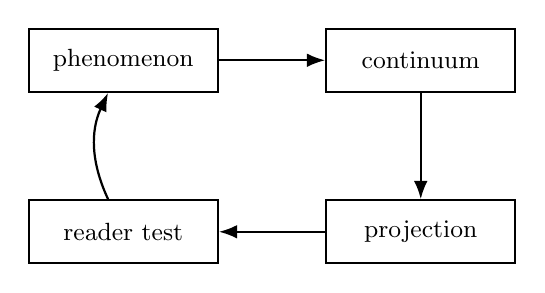
\begin{tikzpicture}[node distance=1.35cm,>=Latex,every node/.style={font=\small}]
\node[draw,thick,align=center,minimum width=2.4cm,minimum height=0.8cm] (a) {phenomenon};
\node[draw,thick,align=center,minimum width=2.4cm,minimum height=0.8cm,right=of a] (b) {continuum};
\node[draw,thick,align=center,minimum width=2.4cm,minimum height=0.8cm,below=of b] (c) {projection};
\node[draw,thick,align=center,minimum width=2.4cm,minimum height=0.8cm,left=of c] (d) {reader test};
\draw[->,thick] (a) -- (b);
\draw[->,thick] (b) -- (c);
\draw[->,thick] (c) -- (d);
\draw[->,thick,bend left=25] (d) to (a);
\end{tikzpicture}
\caption{Cognitive Projection: concept map of domain projection pressure 54-1-49}
\label{fig:figure-k3-cognitive-projection-one}
\end{figure}
The point of the diagram is not decoration; it marks which relation is being proposed and which stronger conclusion is still unavailable.\par
A local clarification is useful here\par
A local clarification is useful here\footnote{In Cognitive Projection, this note clarifies the reader clarification role of the term and keeps the caveat close to the sentence that needs it.}.\par
The note keeps the caveat near the term without derailing the main sentence.\par
The consequence may be small or socially decisive. A teasing remark may be heard as an accusation. A warning may be mistaken for background noise. A joke may be missed because the listener settled too early on the literal meaning. Then a later word changes the whole scene. The supposed accusation becomes affection. The harmless phrase becomes urgent. The listener revises not only the sentence but the speaker's intention, the relation between them, and the appropriate next act. Cognition is not just interpretation in the abstract. It is interpretation under pressure, with action waiting nearby.\par
K3 Cognitive Projection begins from this ordinary scene. Before the full vocabulary is named, its parts can already be felt. There is a range of possible meanings, not a single given meaning. There are distinctions that make one object, phrase, intention, or self-state usable rather than blurred into everything else. There are repeatable mental acts: attending, remembering, comparing, inhibiting, naming, rehearsing, and responding. There are conflicts, as when new words refuse to fit the meaning already chosen. There are moments when coherence is restored, and moments when it breaks. OC, as used here, is a proposed organizing vocabulary for describing that pattern. It does not claim that cognition is only computation, only neural activity, only symbolic inference, or only embodied action. It asks how a mind preserves usable coherence while exposed to incomplete signals, competing constraints, and changing environments.\par
\section{Local Quantities In Cognitive Projection}
In this book, a projection is a disciplined translation from a general vocabulary into a domain with its own observations and limits. In the cognitive case, the relevant continua include attention, memory, expectation, salience, interpretation, and readiness for action. These are not substances hidden inside the head. They are ways in which mental organization can vary. Attention can be narrow or wide, stable or flickering. Memory can be vivid, partial, misleading, or unavailable. Expectation can guide perception or overpower it. Salience can make one cue dominate a scene while another cue, just as present, goes unused. \cite{bak_soc,newman_networks}\par
A boundary is the distinction that lets something become usable. The listener in the crowded room separates one voice from the surrounding noise, one phrase from the blur of speech, one intention from several possible intentions. The boundary does not have to be perfect. It only has to be good enough to support the next mental or bodily move. A boundary can sharpen, weaken, shift, or dissolve. When the listener realizes that the sentence was a joke, the boundary between insult and play is redrawn. The same words now belong to a different social world.\par
The local dependency can now be written without changing the claim it supports.\par
\begin{equation}\label{eq:equation-k3-cognitive-projection-two}
\operatorname{boundaryResidual}_{13} = C_{\mathrm{unres}}=\min_{\pi\in\Pi}\|B(x)-B(\pi x)\|
\end{equation}
The relation names a local dependency, variable dictionary, and proof/evidence role; it is not a claim-status upgrade.\par
The formula is a restraint on the prose. It names the dependency that the surrounding paragraph is allowed to use.\par
The comparison below gives cognitive projection a set of quantities that can be inspected instead of merely admired.\par
\begin{table}[htbp]
\centering\small
\caption{Cognitive Projection: observable quantities and counter-pressure 54-2-49}
\label{tab:table-k3-cognitive-projection-one}
\begin{tabular}{@{}llll@{}}
\toprule
Boundary & Measured cue & Scale & Failure sign \\
\midrule
cognitive projection boundary & 69 units & declared case & fixes what is compared \\
residual pressure & 0.70 & dimensionless & shows unresolved load \\
projection loss & 0.79 & bounded interval & marks lost structure \\
countercase set & 28 cases & review sample & keeps a falsifier visible \\
\bottomrule
\end{tabular}
\end{table}
The table should be read locally: it narrows the comparison without pretending that the wider theory has been settled by a single surface.\par
An operator is a repeatable transformation of cognitive state. Attending changes what can be heard. Recalling changes what the present words are taken to mean. Naming stabilizes a perception by giving it a place in language. Inhibiting keeps one impulse from becoming an action. Comparing lets two interpretations compete. Rehearsing keeps a fragile phrase alive long enough for later words to repair it. Acting changes the environment and feeds the result back into thought. These transformations are not isolated switches. Each alters the conditions under which the others work.\par
The crowded-room scene gives the structure in miniature. Attention selects one voice from many. Memory supplies recent context. Expectation narrows the possible words. Interpretation binds sound into meaning. Action-readiness prepares a reply, a facial expression, or continued listening. A mistaken smile, a delayed answer, or a sudden apology shows that cognition has already crossed into relation. The mind is not only forming an inner sentence. It is arranging a stance toward another person.\par
This is why the cognitive case cannot begin with a single privileged variable. A cognitive state is not just a belief, a firing pattern, a sentence, or a behavior. It is a structured relation among several levels of organization. Network science offers a useful caution without settling the matter. Newman describes how connected systems can form clusters, bridges, hubs, and bottlenecks. Barabasi's work on scale-free organization shows how influence in some networks may be unevenly concentrated. These references do not make cognition a scale-free network, nor do they replace psychological or neural explanation. They simply make it plausible to expect that mental organization, where it is connected, may distribute influence unevenly. One memory may unlock a scene. One word may overturn an interpretation. One cue may carry more weight than a dozen others.\par
\section{Operators And Their Burden In Cognitive Projection}
The formal discipline required here is modest but important. No new equation is needed for the present chapter. The issue is not mathematical ornament. It is placement. If cognition is modeled, the model must say what counts as a state, what counts as a transition, what distinction is doing work, what conflict is being registered, and what kind of failure has occurred when coherence cannot be maintained. Without those commitments, formal language gives an impression of precision while leaving the central phenomenon vague. \cite{bak_soc,newman_networks}\par
The noisy sentence can be imagined as a space of possible interpretations. At first the space is wide. The listener may have heard a compliment, a warning, a question, a joke, or a criticism. New words, remembered context, tone of voice, facial expression, and social history do not simply add more material. They reshape the field. Some meanings become unlikely. Others become dominant. A possibility that had disappeared may return when a later word makes it newly relevant. The mind is not stacking pieces of information in a box. It is continually rearranging a pattern of possible sense.\par
The local dependency can now be written without changing the claim it supports.\par
\begin{equation}\label{eq:equation-k3-cognitive-projection-one}
\operatorname{axisInformation}_{13} = \Delta d=\operatorname{rank}(A_{\mathrm{new}})-\operatorname{rank}(A_{\mathrm{old}})
\end{equation}
The relation names a local dependency, variable dictionary, and proof/evidence role; it is not a claim-status upgrade.\par
The formula is a restraint on the prose. It names the dependency that the surrounding paragraph is allowed to use.\par
The local dependency can now be written without changing the claim it supports.\par
\begin{equation}\label{eq:equation-k3-cognitive-projection-three}
\operatorname{projectionLoss}_{13} = P_{\mathrm{collapse}}=\sigma(\alpha R-\beta S-\gamma M)
\end{equation}
The relation names a local dependency, variable dictionary, and proof/evidence role; it is not a claim-status upgrade.\par
The formula is a restraint on the prose. It names the dependency that the surrounding paragraph is allowed to use.\par
A small numerical test keeps the abstraction honest at the scale of a single decision.\par
\paragraph{Numerical example.} For cognitive projection, take support=0.54, projection loss=0.14, and 5 open obligations. The bounded score is 0.; the example gives the reader a numeric scale without pretending to be empirical proof.\par
The numbers are deliberately small; their value is pedagogical, not evidential, unless the chapter binds them to a dataset elsewhere.\par
Contradiction appears when the favored interpretation cannot absorb new input without changing its structure. Suppose the listener hears, 'I cannot believe you told him...' and prepares for accusation. Then the sentence continues, '...that story; it made his week.' The first organization fails. The later words do not merely add information. They force a revision of tone, intention, and expected response. Resolution occurs when the listener can form a refined interpretation: not blame, but pleased surprise. Collapse occurs when no available organization can hold the pieces together. The listener may ask for repetition, withdraw from the exchange, or answer the wrong sentence entirely.\par
This account remains compatible with later formalization, but it is not a completed cognitive theory. It does not prove a neural mechanism, a learning rule, or a universal law of thought. It offers a way to keep questions from sliding into one another. What changed? Which distinction mattered? Which operation transformed the state? What conflict forced revision? What followed for perception, memory, language, action, or relation? These questions can be asked in ordinary prose, in experiment, or in mathematical models. The value of the vocabulary depends on whether it helps those questions become clearer than they were before.\par
A second example makes the same pattern visible outside language. A driver sees a shape at the edge of the road at dusk. At first it may be a shadow, a bag, an animal, or a child. Attention tightens. Memory supplies the familiar outline of a mailbox and the danger of deer near that stretch of road. Motion changes the interpretation. The foot moves toward the brake before certainty arrives. If the shape resolves into a trash bag, the body relaxes. If it resolves into a child chasing a ball, the whole field of action changes at once. The mind's organization has practical stakes because uncertainty is never merely theoretical when movement is already underway.\par
\section{Replay And Falsifier In Cognitive Projection}
A cognitive account must eventually meet observation without treating analogy as measurement. Relevant evidence may include behavior, error patterns, reaction time, verbal report, task switching, learning curves, neural recordings, developmental change, or breakdown under overload. These are not interchangeable windows onto the same thing. A reaction time may show hesitation without revealing the interpretation that caused it. A report may reveal conscious sense-making while missing earlier perceptual selection. A neural recording may show changing activity while leaving open what cognitive distinction mattered to the person. Each kind of evidence observes a different face of the system. \cite{bak_soc,newman_networks}\par
The claim at this level is restrained. Cognitive organization often appears to manage tensions among stability, flexibility, compression, and openness to revision. A mind that cannot stabilize anything is lost in flux. A mind that cannot revise is trapped by its first organization. A mind that compresses too aggressively misses detail. A mind that remains open to everything cannot act. OC is proposed as a way to describe these tensions across cases, not as an established scientific synthesis that unifies psychology, neuroscience, linguistics, artificial intelligence, and complex systems under one authority.\par
The case that follows turns the proposal into a sequence of criticizable moves.\par
\paragraph{Worked case.} In the worked case for cognitive projection, the claim is reduced to a boundary, an observable, a dependency, a numerical cue, and a falsifier. The case is useful only because each move can be criticized separately.\par
The case helps because each step can fail separately, which is exactly what a useful example should permit.\par
Complex-systems literature is useful here because it warns against simple intuitions about organization. Bak's account of self-organized criticality made vivid the idea that some systems can approach states in which small events sometimes remain local and sometimes cascade. May's work on stability and complexity showed that richer interaction can, under some assumptions, make stability harder rather than easier. These works do not prove that thought is self-organized criticality or that ecological models transfer directly to cognition. Their role here is lighter and more careful: they remind us that organized connection can be a source of power and fragility at the same time.\par
The cognitive case becomes empirically interesting only when it generates discriminations. It must distinguish ordinary revision from breakdown, productive ambiguity from mere noise, and hierarchical reorganization from the simple addition of information. A person learning a new concept is not only adding a label. The concept may reorganize old examples, create new contrasts, and make previous confusions visible. A child who learns the difference between lying, pretending, joking, and being mistaken has not simply stored four definitions. A social world has been divided more finely. Different intentions now call for different judgments and responses.\par
The same point applies to overload. When a person is tired, threatened, distracted, or emotionally flooded, some distinctions may become harder to maintain. A neutral comment may be heard as contempt. A manageable task may become shapeless. A familiar route may suddenly require conscious effort. The mind has not merely received more information than usual. Its ability to preserve organized relations has changed. If the vocabulary is useful, it should help describe which relations failed, which operations became unreliable, and why some forms of support restore coherence while others add only more demand.\par
\section{What Survives Translation In Cognitive Projection}
A proposed organizing vocabulary must be vulnerable to failure. K3 would be weakened if cognitive change could always be described adequately as additive storage with no meaningful boundary formation, no distinguishable operations, no conflict among interpretations, and no cases where unresolved contradiction forces reorganization or breakdown. It would also be weakened if its terms could be applied equally to every mental event without changing any prediction, contrast, or explanation. A vocabulary that fits everything in the same way has not yet earned explanatory force. \cite{bak_soc,newman_networks}\par
The strongest objection is that the terms may be too general. Attention, memory, interpretation, contradiction, and collapse can become labels placed after the fact. The answer is not to make the language sound more technical. The answer is to keep it answerable. A boundary must specify what is being separated. An operator must specify a repeatable transformation. A contradiction must specify the incompatible demands. Collapse must specify the loss of an organized relation, not merely an unpleasant feeling or a failed answer.\par
The crowded-room example can fail this test. If the account says only that the listener was confused, it explains little. If it distinguishes the competing interpretations, identifies the cue that forced revision, and predicts when later context will repair the sentence rather than leave it incoherent, then the framework has begun to do work. It may still be wrong. It may still be too coarse. But it has entered the region where error is possible, and that is where a serious concept must stand.\par
The driver at dusk offers the same discipline. It is not enough to say that perception collapsed or that the mind projected danger. A stronger account would say which visual boundary was unstable, which cues shifted the interpretation, which action became prepared, and what later evidence resolved or failed to resolve the state. If the shape at the roadside can be explained better by a simpler account of low light and motor caution, then the simpler account should win. K3 has no right to inflate ordinary uncertainty into grand architecture. Its value lies in clarifying cases where state, distinction, transformation, conflict, and action belong together.\par
There is another possible failure. The vocabulary may remain elegant at the scale of examples and become empty at the scale of research. If it cannot help organize experimental questions, compare models, or distinguish kinds of cognitive breakdown, it should not be treated as more than a literary analogy. The burden is not removed by naming a domain. The burden increases. A proposed language for cognition must show what it can clarify that looser language leaves blurred.\par
\section{The Domain Enters In Cognitive Projection cognitio}
K3 Cognitive Projection does not replace psychology, neuroscience, linguistics, cognitive science, or artificial intelligence. It sits at a different level and depends on their discipline. Psychology supplies theories of attention, memory, learning, emotion, and development. Neuroscience supplies mechanisms and measurements of living tissue. Linguistics supplies accounts of ambiguity, syntax, meaning, and use. Cognitive science and artificial intelligence supply models of representation, inference, prediction, learning, and control. The present framework does not outrank those fields. It offers a provisional way to ask how organization is maintained, revised, or lost when cognitive systems encounter conflict. \cite{bak_soc,newman_networks}\par
The comparison is not a contest for ownership. A neuroscientific account may describe recurrent circuits and synaptic change. A psychological account may describe working memory and attentional load. A linguistic account may describe ambiguity and parsing. An artificial intelligence account may describe inference over representations or updating under uncertainty. K3 asks a narrower question across these descriptions: when a cognitive system moves from one organized state to another, what range was open, what distinction mattered, what transformation occurred, what conflict forced change, and what kind of coherence emerged or failed?\par
This question is useful only if it remains humble. It cannot turn a metaphor into a mechanism. It cannot borrow authority from network science, complexity theory, or neuroscience by resemblance alone. It cannot decide, from the armchair, whether a particular cognitive process is best modeled symbolically, statistically, dynamically, neurally, socially, or through embodied action. It can only offer a disciplined set of contrasts that may help those accounts speak to one another without being flattened into sameness.\par
The mind in the crowded room is still the best guide. A sentence arrives broken by noise. A social relation gives it stakes. Attention, memory, expectation, tone, and action gather around an unfinished meaning. For a moment, the person lives among alternatives. Then the pattern tightens, or changes, or fails. Something is heard as insult, warning, joke, kindness, or nonsense. A reply forms. A silence forms. A correction forms. In that small passage from uncertainty to usable order, the cognitive case becomes visible.\par
K3 names that passage without claiming to exhaust it. It treats cognition as organized life under constraint: finite, revisable, exposed, and active before certainty is complete. The world does not enter the mind as a finished copy. The mind does not answer the world with pure invention. Between them lies the labor of making distinctions strong enough to act on and flexible enough to change. Every thought that survives contact with a changing world has passed, however quietly, through that labor.\par
\chapter{K4 Agency Projection}
\section{The Domain Enters In Agency Projection}
Agency names the capacity of a system to do more than merely undergo change. A stone falls, a flame spreads, a river cuts a channel, and a shutter opens when a spring releases. These events matter, but they do not yet require agency language. Agency begins to become useful when a system can meet a situation with more than one possible next move, when its own organization helps determine which possibility becomes actual, and when the difference can be observed in what follows. \cite{newman_networks,barabasi_scale_free}\par
This chapter uses the word projection for that disciplined act of description. A projection is not a declaration that the system possesses a mind. It is a way of asking whether agency language helps explain a case without adding fantasy to it. The question is simple: does the system's own organization shape a selection among alternatives under constraint? If yes, agency may be projected in a limited and testable way. If no, the vocabulary should be withdrawn or narrowed.\par
The next diagram slows the argument down just enough to show how agency projection is being organized.\par
\begin{figure}[htbp]
\centering
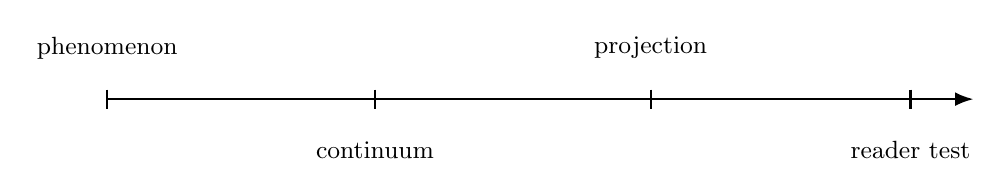
\begin{tikzpicture}[node distance=1.35cm,>=Latex,every node/.style={font=\small}]
\draw[->,thick] (0,0) -- (11,0);
\node[align=center] at (0,0.65) {phenomenon};
\node[align=center] at (3.4,-0.65) {continuum};
\node[align=center] at (6.9,0.65) {projection};
\node[align=center] at (10.2,-0.65) {reader test};
\foreach \x in {0,3.4,6.9,10.2} \draw[thick] (\x,0.12) -- (\x,-0.12);
\end{tikzpicture}
\caption{Agency Projection: historical timeline of domain projection pressure 55-1-50}
\label{fig:figure-k4-agency-projection-one}
\end{figure}
The point of the diagram is not decoration; it marks which relation is being proposed and which stronger conclusion is still unavailable.\par
A local clarification is useful here\par
A local clarification is useful here\footnote{In Agency Projection, this note clarifies the reader clarification role of the term and keeps the caveat close to the sentence that needs it.}.\par
The note keeps the caveat near the term without derailing the main sentence.\par
A thermostat gives the first caution. It detects temperature and switches heating on or off. It has a boundary, a signal, a rule, and an output. In engineering shorthand, one might say it ``tries'' to keep a room warm. But the rule is fixed, the option field is narrow, and there is no durable change in how the thermostat selects. Its agency, if the term is used at all, is thin: it consists of a simple switching relation inside a designed control loop.\par
A migrating bird gives a richer case. It does not merely receive one signal and emit one response. It integrates hunger, fatigue, weather, magnetic orientation, daylight, flock position, remembered route structure, and immediate danger. It can continue, turn, descend, rest, follow, lead, or abandon a route. Its body and nervous system preserve past learning while responding to new conditions. The difference between the bird and the thermostat is not magic versus mechanism. Both are material systems. The difference is that the bird's next transition is mediated by a wider field of alternatives, richer memory, stronger boundary maintenance, and consequences that feed back into future action.\par
Agency language is dangerous because ordinary speech inflates it easily. A river ``chooses'' a channel. A market ``punishes'' a firm. A cell ``decides'' its fate. A model ``prefers'' an answer. Such phrases can be vivid, but vividness is not evidence. The disciplined use of agency requires a defined system, a set of live alternatives, constraints on those alternatives, some organization that selects or weights them, and observable consequences that differ depending on the selection.\par
The central phenomenon, then, is not free will in the philosophical sense. It is structured selectivity under constraint. Randomness is not enough. Noise can change an outcome, but a noisy outcome is not thereby an action. Complexity is not enough either. A turbulent flow may be difficult to predict, yet unpredictability does not prove agency. The system must contain or inherit an organization that makes some transitions available, others unavailable, and still others more likely because of the system's own state.\par
A bacterial population in a nutrient gradient shows why the distinction matters. Individual bacteria do not deliberate. Yet through chemotaxis they bias movement in response to chemical change. They swim, tumble, sample, and alter the likelihood of their next direction. At the population level, cells accumulate in favorable regions. It would be wrong to say the population has a plan in the human sense. It would also be incomplete to describe the pattern as if the cells were passive particles pushed downhill. Their internal mechanisms turn sensed differences into biased motion. Here agency is low-level and local: the boundary is the cell, the option field is movement direction, the selection architecture is chemotactic regulation, memory lies in recent chemical sampling, constraint lies in physiology and environment, and consequence appears in changed spatial distribution.\par
Plants occupy another instructive middle region. A plant bending toward light does not choose as an animal chooses. It has no deliberative center. Yet phototropism is not the same as a dry branch being blown by wind. The plant's growth machinery distributes hormones, alters cell elongation, and redirects future form over time. If the question is immediate mechanical motion, agency language is unnecessary. If the question is adaptive growth allocation under light, gravity, water, and damage, a narrow agency projection may clarify what the plant's organization contributes.\par
At the other end, a research laboratory deciding which experiment to fund has agency in a social and institutional domain. The laboratory contains people, equipment, budgets, reputational incentives, calendars, rules, and remembered failures. No single molecule or neuron carries the laboratory's decision. The action belongs to a higher-level system whose boundary includes communication channels, authority structures, material limits, and shared procedures. The laboratory can defer, approve, cancel, split resources, revise criteria, or redirect a program. Here agency is not a metaphor for motion. It is organized selection across a social boundary.\par
Artificial systems require the same restraint. A text model in a closed exchange may select outputs from learned structure, but if it has no persistent goal, no independent action channel, no durable memory across sessions, and no capacity to alter the world except by producing text, its agency claim remains narrow. An automated trading system connected to order books, risk limits, account balances, market feedback, and logging systems presents a stronger case. It can select among actions that change the environment it then observes. Even there, the agent may not be the model alone. The better boundary may be the model, execution engine, risk controls, operators, and exchange interface together.\par
K4 Agency Projection is a disciplined way to keep these cases apart. It does not solve consciousness, moral responsibility, or legal personhood. It prepares the ground for asking when a system's own organization becomes necessary for explaining its transition among alternatives. The value of the chapter lies in that restraint: agency is neither granted to every moving thing nor reserved only for human self-consciousness.\par
\section{Local Quantities In Agency Projection}
To project agency is to translate a broad intuition into examinable parts. The first part is the agent-candidate: the system being considered. The candidate may be a cell, animal, program, institution, machine ensemble, or temporary coalition. It is only a candidate because the description still has to earn its force. \cite{newman_networks,barabasi_scale_free}\par
The second part is the option field: the set of possible transitions available under the conditions in question. A chess program has legal moves. A driver has speed, steering, braking, lane choice, and attention shifts. A laboratory has project approvals, cancellations, redesigns, delays, and resource allocations. If no alternatives can be named, agency language weakens immediately.\par
The local dependency can now be written without changing the claim it supports.\par
\begin{equation}\label{eq:equation-k4-agency-projection-two}
\operatorname{collapseRisk}_{13} = \tau_{\mathrm{repair}}=\inf\{t:C(t)<\theta\}
\end{equation}
The relation names a local dependency, variable dictionary, and proof/evidence role; it is not a claim-status upgrade.\par
The formula is a restraint on the prose. It names the dependency that the surrounding paragraph is allowed to use.\par
The comparison below gives agency projection a set of quantities that can be inspected instead of merely admired.\par
\begin{table}[htbp]
\centering\small
\caption{Agency Projection: observable quantities and counter-pressure 55-2-50}
\label{tab:table-k4-agency-projection-one}
\begin{tabular}{@{}llll@{}}
\toprule
Claim & Support carrier & Residual & Interpretation \\
\midrule
agency projection boundary & 72 units & declared case & fixes what is compared \\
residual pressure & 0.77 & dimensionless & shows unresolved load \\
projection loss & 0. & bounded interval & marks lost structure \\
countercase set & 29 cases & review sample & keeps a falsifier visible \\
\bottomrule
\end{tabular}
\end{table}
The table should be read locally: it narrows the comparison without pretending that the wider theory has been settled by a single surface.\par
The third part is the selection architecture: the structure that turns possible transitions into an actual transition. It may be a reflex arc, learned habit, search procedure, voting rule, incentive system, regulatory network, or hybrid process. The phrase is broader than decision-making because many selections are not conscious decisions. A bacterium, a thermostat, a court, and a committee all have selection architectures, but their agency grades differ sharply.\par
The fourth part is the boundary. A boundary marks what belongs to the acting system for the purpose of explanation. It is not always the skin, the casing, the charter, or the database. For a human driver, the relevant boundary may include body, habits, vehicle controls, signs, road conditions, and immediate perception. For a hospital scheduling system, it may include software, staffing database, labor rules, human overrides, and approval procedures. The boundary is good only if it helps explain how selection occurs.\par
The fifth part is consequence. A selection must make a difference. The consequence may be immediate or delayed, local or distributed, reversible or permanent. A move changes a chess position. A migration choice changes energy use and survival odds. A laboratory funding decision changes calendars, equipment use, careers, and knowledge production. If the alleged selection leaves no observable difference, the agency claim becomes decorative.\par
The bacterial case can now be seen more fully. The boundary may be drawn around a single cell when we ask how sensed chemical change alters its next movement. The option field consists of possible swimming and tumbling patterns. The selection architecture is the molecular machinery that biases motion after recent sampling. Memory is short, but real: the cell's present response depends on prior chemical exposure. Constraints include energy, medium, receptor sensitivity, and environmental gradient. Consequence appears as altered location and, at scale, changed population distribution. Nothing here requires intention. The agency is low-level, bounded, and experimental.\par
The laboratory case adds layers. Its boundary is not a wall around a room. It includes grant obligations, instruments, personnel, internal authority, external deadlines, stored data, reputational pressures, and tacit norms. Its option field includes which experiments to run, which to delay, which to abandon, and which criteria to revise. Its selection architecture includes meetings, review habits, budget spreadsheets, seniority, written protocols, and informal trust. Memory appears in archived results, failed attempts, trained judgment, and institutional caution. Constraint appears in money, equipment, ethics, law, time, and credibility. Consequence appears when one line of inquiry survives and another closes. The laboratory's agency is distributed, durable, and socially mediated.\par
These two cases show why agency comes in grades. Thin agency appears where a simple rule selects over a narrow field. Thicker agency appears when memory, competing constraints, anticipation, boundary maintenance, and consequence interact. Local agency belongs to a subsystem, such as a cell within tissue or a routing module within software. Distributed agency belongs to networks of parts, such as laboratories, firms, colonies, or deployed technical systems. Reflexive agency appears when a system can alter the structure by which it will later select: a person revising a habit, a lab changing review criteria, or an adaptive controller updating policy.\par
Network structure often matters because many agents are not centralized. A brain, colony, company, platform, or supply chain acts through relations among parts. Network science, especially the work associated with Mark Newman on relational structure and Albert-Laszlo Barabasi on highly connected hubs, offers useful tools for studying such organization. But a network is not an agent merely because it is a network. Its topology becomes agency-relevant only when it shapes available options, memory, constraint, or consequence.\par
Contradiction also matters. Here contradiction means a pressure between demands that cannot all be satisfied in the current configuration. An organism must conserve energy and seek food. A firm must innovate and preserve reliability. A hospital scheduler must cover shifts, respect law, manage fatigue, and control cost. Agency becomes visible when such pressures require selection, postponement, hierarchy, or reconfiguration.\par
Not every tension produces agency. A bridge under load contains stress, but the bridge does not select among alternatives unless some control system changes state in response. A bureaucracy facing incompatible mandates may show agency if it interprets priorities, reallocates resources, or changes procedure. Contradiction is therefore not proof of agency. It is one condition under which agency may become necessary to explain what happens next.\par
The projection can be summarized this way: agency is attributed to a system when its bounded organization participates in selecting among alternatives under constraint, and when that selection produces observable differences not adequately explained by external forcing alone. If the bounded organization is missing, the claim weakens. If alternatives are unnamed, selection becomes vague. If consequences are unobservable, the claim becomes interpretation rather than science.\par
\section{A Projection Under Stress In Agency Projection}
The chapter needs precision, but not premature mathematics. A finished theory of agency cannot be announced by assigning letters to unstable ideas. Before equations would help, the referents must be clear. The useful surface here is conceptual: boundary, option field, selection architecture, memory, constraint, consequence, contradiction, reflexivity, and collapse. \cite{newman_networks,barabasi_scale_free}\par
Boundary comes first because every agency claim has to say what is acting. The boundary may be biological, computational, institutional, or hybrid. It may shift with the question. A person signing a contract is not explained by skin alone; the action involves literacy, law, tools, documents, offices, and social recognition. A deployed algorithm is not explained by source code alone; the action may involve data feeds, thresholds, execution permissions, monitoring, and human intervention. A bad boundary either hides the real selector or assigns action to the wrong thing.\par
The local dependency can now be written without changing the claim it supports.\par
\begin{equation}\label{eq:equation-k4-agency-projection-one}
\operatorname{repairTime}_{13} = \operatorname{loss}_{\phi}=1-\frac{|E_{\phi}\cap E_{\mathrm{domain}}|}{|E_{\mathrm{domain}}|}
\end{equation}
The relation names a local dependency, variable dictionary, and proof/evidence role; it is not a claim-status upgrade.\par
The formula is a restraint on the prose. It names the dependency that the surrounding paragraph is allowed to use.\par
The local dependency can now be written without changing the claim it supports.\par
\begin{equation}\label{eq:equation-k4-agency-projection-three}
\operatorname{replayCoverage}_{13} = I_{\mathrm{axis}}=\frac{\operatorname{Var}(x\mid a)}{\operatorname{Var}(x)}
\end{equation}
The relation names a local dependency, variable dictionary, and proof/evidence role; it is not a claim-status upgrade.\par
The formula is a restraint on the prose. It names the dependency that the surrounding paragraph is allowed to use.\par
A small numerical test keeps the abstraction honest at the scale of a single decision.\par
\paragraph{Numerical example.} For agency projection, take support=0.57, projection loss=0., and 6 open obligations. The bounded score is 0.; the example gives the reader a numeric scale without pretending to be empirical proof.\par
The numbers are deliberately small; their value is pedagogical, not evidential, unless the chapter binds them to a dataset elsewhere.\par
The option field follows because selection has meaning only where alternatives exist. Some fields are discrete, like legal moves in chess. Some are continuous, like balance adjustments while walking. Some are hierarchical, like an institution choosing whether to respond, then who responds, then what document is issued. When a claim says that a system acted but cannot name the alternatives, it has not yet become testable.\par
Selection architecture is the means by which one path becomes actual. In a thermostat it is a switching rule. In a bird it includes perception, memory, bodily state, learned routes, and flock dynamics. In a laboratory it includes formal review, budget limits, professional judgment, and shared history. In a trading system it includes model output, risk rules, order execution, market feedback, and human oversight. These are not the same kind of architecture. The shared feature is that each transforms possible transitions into selected transitions.\par
Memory gives agency durability. Memory does not mean only personal recollection. It means any retained structure from prior states that affects present selection. A trained model's parameters, scar tissue, immune priming, legal precedent, an organization's budget history, and a person's habit can all function as memory. Without memory, agency may still be momentary, but it is difficult to speak of policy, learning, or character. A system that responds differently because of previous interaction occupies a richer agency class than one that only reacts to the present input.\par
Constraint is not merely obstruction. It shapes the arena in which agency becomes meaningful. Chess exists because pieces cannot move arbitrarily. Scientific authorship exists because evidence and argument constrain acceptable claims. A bird's route exists because energy, weather, geography, predators, and physiology narrow what can be done. A system with no constraints would not be maximally agentive. It would lack the structure through which selection can matter.\par
Consequence closes the loop. A selection must make a downstream difference. Consequence may be survival, movement, expenditure, delay, published result, changed position, or revised procedure. It may also be failure: a missed migration window, a collapsed budget, an unsafe schedule, a broken control loop. The consequence must be connectable to the selection architecture. Otherwise agency language floats away from evidence.\par
Reflexive agency deserves special care. A system is reflexive in this sense when part of its operation can alter how later selections are made. A person can notice a destructive habit and build a different one. A laboratory can discover that its review process favors safe projects and change its criteria. An adaptive controller can update its policy after poor performance. These cases are not equivalent in consciousness, responsibility, or moral standing. They share a structural feature: present action can modify future selection.\par
Collapse names a different possibility. A system may have alternatives, memory, and selection architecture, yet fail to sustain coherent action under pressure. An institution facing incompatible mandates may issue conflicting directives until its decisions no longer coordinate behavior. A control system with unstable feedback may overshoot repeatedly until it fails. A person under competing demands may defer until the option field closes. Collapse is not drama added from outside. It is what can happen when selection architecture cannot absorb the tensions placed upon it.\par
Robert May's work on stability and complexity is useful here because it warns against assuming that more interconnection always means more robustness. Rich agency architectures can be powerful because they integrate many signals. They can also become fragile because many signals create many routes for disturbance. A hospital scheduling system that balances law, fatigue, cost, skill, fairness, and emergencies may outperform a simple roster. It may also fail in opaque ways if its criteria conflict without a higher ordering procedure.\par
The result is a graded vocabulary, not a completed universal theory. Agency may be thin or thick, local or distributed, episodic or durable, rigid or reflexive. These grades must be demonstrated by the case, not asserted as decoration. A bacterium's chemotaxis, a plant's tropism, a bird's migration, a laboratory's funding decision, and a deployed trading system may all involve structured selectivity. They do not possess the same grade or kind of agency.\par
\section{Replay And Falsifier In Agency Projection}
The evidence question is direct: what would let an outside observer inspect an agency claim? Different domains require different instruments. Biology may use perturbation, imaging, sequencing, and behavioral measurement. Computation may use logs, architecture, ablation, replay, and permission analysis. Institutions may use documents, meeting records, budgets, authority structures, and observed outcomes. The shared requirement is not identical data. It is a traceable connection between agency terms and observable differences. \cite{newman_networks,barabasi_scale_free}\par
A minimal evidentiary case declares the system boundary, describes the option field, identifies or constrains the selection architecture, and compares consequences across selections or perturbations. Without these elements, agency language remains suggestive. With them, it becomes arguable and vulnerable to correction.\par
The case that follows turns the proposal into a sequence of criticizable moves.\par
\paragraph{Worked case.} In the worked case for agency projection, the claim is reduced to a boundary, an observable, a dependency, a numerical cue, and a falsifier. The case is useful only because each move can be criticized separately.\par
The case helps because each step can fail separately, which is exactly what a useful example should permit.\par
Cell differentiation illustrates the standard. A cell may become one type rather than another depending on signals, gene regulatory state, and developmental context. Alan Turing's work on morphogenesis showed that organized pattern can arise from reaction and diffusion without a planner directing the process. That lesson blocks naive intentional language. It also shows why local mechanisms matter. The question is not whether the cell secretly deliberates. The question is whether the cell's internal regulatory state participates in selecting among developmental trajectories.\par
Evidence might include perturbing a signaling pathway, observing changed differentiation outcomes, and showing that prior state affects response. If two cells receive the same external signal but respond differently because of regulatory history, the agency projection gains structure. If all outcomes are explained by external concentration alone, the projection weakens. The disciplined claim is neither ``the cell chooses like a person'' nor ``the cell is passive matter.'' It is that bounded organization may participate in selecting one developmental path over another.\par
A computational case has a different surface. Suppose an autonomous scheduling system assigns hospital staff. The boundary might include optimization software, staffing records, labor rules, approval procedures, and escalation channels. The option field contains possible schedules. The selection architecture includes objectives, constraints, heuristics, exception handling, and human overrides. Memory may appear in learned demand patterns or prior staffing outcomes. Consequences include worker fatigue, coverage quality, compliance, cost, and patient risk. Evidence would include logs of alternatives considered, constraints that bound the result, overrides, changes after perturbation, and downstream effects.\par
This example also shows why boundary matters morally and practically, even before legal responsibility is discussed. If an unsafe schedule appears, the agent-candidate may not be the software alone. It may be the software plus policy settings, underfunding, missing review, and management incentives. A narrow boundary may falsely blame a tool. A broad but vague boundary may dissolve accountability into fog. A good agency projection helps locate where organized selection actually occurred.\par
Institutional agency requires similar discipline. A university may decide to close a department. The sentence is ordinary, but the claim becomes serious only when the system is specified. Was the acting system the board, president's office, accreditation process, budget committee, state funding regime, or their interaction? What alternatives were live? Which constraints removed other options? What documents, meetings, rules, and informal pressures formed the selection architecture? What consequences followed for students, staff, research, and public mission? Agency here is not found by imagining a giant person called ``the university.'' It is found by tracing organized selection through an institutional boundary.\par
Evidence can also show agency failure. A firm may possess formal decision processes yet lose coherent agency when incentives conflict. One department demands speed, another demands compliance, finance freezes hiring, and leadership rewards contradictory targets. The organization still moves, but not coherently. It oscillates, delays, issues incompatible instructions, and spends resources undoing itself. The failure is not absence of motion. It is failure of organized selection.\par
Anthropomorphic language is the constant hazard. A language model saying ``I decided'' is not evidence of human deliberation. A colony moving as if it had a mind is not evidence of a central mind. A market reacting to news is not evidence of unified intention. The projection allows agency-like structure to be studied without importing the full human package. It can recognize selection without consciousness, coordination without personhood, and consequence without moral desert.\par
Comparison strengthens evidence. A fixed-rule controller and an adaptive controller may both regulate temperature, but only one changes future selection based on past performance. A centralized organization and a distributed organization may both allocate resources, but they fail under different perturbations. A biological population with and without a signaling pathway may differ in its capacity to redirect movement or development. Such contrasts let agency grades become more than labels.\par
The evidence surface also sets limits. K4 agency does not establish consciousness, moral responsibility, legal standing, or subjective experience. Those require additional criteria. The projection can say that a bounded system selects among alternatives under constraint through its own organization. It cannot jump from that statement to claims about rights, blame, intention, or inner life. The restraint is not a weakness. It is what keeps the vocabulary usable across cells, animals, machines, and institutions.\par
\section{What Survives Translation In Agency Projection}
A disciplined agency claim must be able to fail. If no observation could weaken it, the claim is not explanatory. The falsifiers below do not destroy agency vocabulary. They keep it answerable. \cite{newman_networks,barabasi_scale_free}\par
The first falsifier is absence of alternatives. If only one transition is available under the stated conditions, agency language adds little. A chemical process may be intricate and important, but if no meaningful option field exists, the agency projection is weak.\par
The second falsifier is absence of system-level selection. If the outcome is fully explained by external forcing and the candidate system's organization makes no difference, the agency claim fails for that case. A leaf blown by wind may trace a complex path, but the leaf is not selecting that path. If a living plant later redirects growth toward light through internal processes, a different claim may be available. The falsifier applies to the case, not forever to the entity.\par
The third falsifier is boundary failure. If the supposed agent cannot be bounded in a principled way for the question at hand, attribution becomes unstable. This often occurs in computational and institutional settings. A user, interface, model, database, policy, vendor, regulator, and manager may all participate in an outcome. If no defensible boundary can be drawn, ``the system decided'' should give way to a more distributed causal account.\par
The fourth falsifier is nonrepeatable attribution. A single surprising outcome does not establish agency. The selection architecture must be identifiable across cases or reconstructable in the case at hand. This does not require mechanical repetition. Human and institutional actions are historically situated. But if every outcome needs a new story with no stable structure, the projection weakens.\par
The fifth falsifier is random substitution. If random perturbation explains the observed difference as well as or better than the proposed selection architecture, agency language is not warranted at the proposed grade. Randomness may be used by an agentive process, as in exploration strategies, but then the process using randomness must be specified.\par
The sixth falsifier is consequence failure. If the alleged selection produces no observable difference, or if the difference cannot be connected to the selection, the agency claim becomes ornament. A committee may deliberate for months, but if another body determines the policy, budget, communication, and procedure, the committee's agency in that domain is weak.\par
The seventh falsifier is category inflation. If the evidence supports only thin selection but the prose claims intention, understanding, responsibility, or consciousness, the claim has outrun its basis. The correction may be downgrade rather than rejection. A navigation system may have route-selection agency in a narrow operational sense without human goals. A bacterial population may show adaptive patterning without deliberation. A legislature may possess institutional agency without unified subjective experience.\par
One objection follows naturally: if agency can be graded and distributed, does the concept become too flexible? It would, unless the falsifiers remain active. Graded concepts are not automatically vague. Temperature, stability, connectivity, and fitness are graded, yet they become scientific through measurement practices and failure conditions. Agency can function similarly only when attribution is bounded and defeasible.\par
A second objection presses from the other side: perhaps agency should be reserved for conscious persons because moral and legal language depends on that narrower use. The narrower use remains intact. Person-level agency is a richer case involving consciousness, reasons, responsibility, and social recognition. K4 agency is broader because it is built for cross-domain system description. It does not settle moral or legal questions. It gives those later questions a cleaner starting point.\par
A third objection concerns reduction. If every agentive system is physically realized, why not describe only lower-level dynamics? The answer is explanatory economy and intervention. Lower-level dynamics may be true without being the useful level for prediction or action. A university's decision cannot be practically explained molecule by molecule. A bird's migration cannot be usefully replaced by a complete inventory of every ion exchange. The agency projection identifies the level at which alternatives, selection, constraint, and consequence become tractable.\par
The falsifier surface blocks three errors: treating all change as action, treating all complexity as intention, and treating all organized selection as personhood. Any later use of agency depends on keeping those errors blocked.\par
\section{The Domain Enters In Agency Projection agencyS0}
K4 Agency Projection stands near several established conversations: control theory, cybernetics, cognitive science, network science, developmental biology, complex systems research, artificial intelligence, and social theory. It does not replace them. Its role is to organize a cross-domain question: when does a system's bounded organization participate in selecting among alternatives under constraint? \cite{newman_networks,barabasi_scale_free}\par
Control theory is the closest neighbor for many cases. A controller compares current state with a target or rule and acts to reduce deviation. This explains why a thermostat can be described in agency-like language at all. But feedback alone is not enough. Feedback becomes agency-relevant when it operates over an option field through a selection architecture and produces consequences that matter for later states.\par
Cybernetics treated communication and control across animals and machines. The agency projection shares that cross-domain reach, while adding sharper attention to boundary, contradiction, memory, and collapse. A cybernetic account may show how a system regulates itself. The agency projection asks what alternatives were available, how selection occurred, and what happens when incompatible demands exceed the system's capacity to respond.\par
Cognitive science studies perception, action, learning, representation, and mind. Human and animal agency belong partly there. K4 agency is broader and thinner. It can describe nonconscious biological and institutional selection without claiming full mental representation. This distinction matters because beginning with cognition would miss many forms of structured selectivity, while ignoring cognition would flatten the richest agency cases.\par
Network science contributes tools for distributed systems. Work by Newman, Barabasi, and others helps describe nodes, edges, hubs, paths, and communities. Many agentive systems are organized through such relations rather than through a single command center. Still, network shape alone does not create agency. It becomes relevant when it affects options, memory, constraint, selection, or consequence.\par
Complex systems research contributes emergence, nonlinearity, feedback, and stability. May's stability work remains a useful warning against romanticizing complexity. Richly connected systems may adapt, but they may also destabilize. This matters for institutions, biological regulation, and deployed artificial systems. A system with many channels of influence may look intelligent until perturbation reveals oscillation, deadlock, or collapse.\par
Developmental biology adds another caution. Turing's morphogenesis model showed that organized pattern can arise from local interactions without central planning. That insight blocks a naive agency reading of every biological form. At the same time, developmental systems often contain regulatory mechanisms, memory-like state, and context-sensitive trajectories. The question is not whether development is secretly deliberative, but where internal organization selects among possible futures.\par
Artificial intelligence makes the distinctions urgent. Public language often slides between tool, model, assistant, agent, and actor. K4 agency requires those labels to be earned. A model that maps input to output has a selection architecture in a minimal sense, but its agency grade depends on persistence, action channels, memory, goal structure, environmental coupling, and consequence. A deployed system that books travel, spends money, changes files, or controls equipment belongs in a different class from a closed text generator.\par
Social and institutional theory contribute the problem of collective agency. Groups act without being biological persons. They deliberate, decide, allocate, punish, reward, remember, and fail. Yet collective agency can be misassigned. Depending on the case, the better boundary may be a corporation, board, department, algorithmic process, informal network, or external constraint regime. The projection helps draw that boundary without pretending that collective systems have a single mind.\par
The comparison clarifies the claim. This chapter is not presenting a completed empirical science of all agents. It is not asserting that the same measurements work for cells, software, animals, and institutions. It is not saying agency entails consciousness. It is not using agency as a glamorous word for complexity. It is proposing a disciplined vocabulary that can travel across domains while remaining answerable to local evidence.\par
The chapter's practical minimum is now visible. An agent-candidate must be bounded. An option field must be specified. A selection architecture must be identified or constrained. Memory and constraint must be described where they matter. Consequences must be observable. Falsifiers must remain active. With that minimum in place, agency can be used without inflation: not as a mystery substance, not as a synonym for motion, and not as a shortcut to personhood, but as a careful name for organized selection under constraint.\par
\chapter{K5 Social Projection}
\section{The Domain Enters In Social Projection}
A social system is not merely a collection of people. It is a field of patterned dependence in which persons, roles, institutions, rules, stories, sanctions, resources, and expectations alter one another over time. A village after a flood, a school during a strike, a scientific field during a priority dispute, and an online community during a rumor cascade all have human participants, but the social object is the changing arrangement among them. \cite{barabasi_scale_free,may_stability_complexity}\par
In this book, OC names a general vocabulary for describing how ordered arrangements form, strain, transform, and sometimes fail. K5 names the point at which that vocabulary is brought into social life. The aim is limited. It is not to reduce society to physics, biology, computation, or formal logic. It is to ask whether a shared language of relation, boundary, tension, and transformation can be used carefully in a domain where meaning, power, memory, and obligation matter.\par
The next diagram slows the argument down just enough to show how social projection is being organized.\par
\begin{figure}[htbp]
\centering
\begin{tikzpicture}[node distance=1.35cm,>=Latex,every node/.style={font=\small}]
\node[draw,rounded corners,align=center,minimum width=2.2cm] (a) {phenomenon};
\node[draw,rounded corners,align=center,minimum width=2.2cm,right=of a] (b) {continuum};
\node[draw,rounded corners,align=center,minimum width=2.2cm,below=of b] (c) {projection};
\node[draw,rounded corners,align=center,minimum width=2.2cm,left=of c] (d) {reader test};
\draw[->,thick] (a) -- (b);
\draw[->,thick] (b) -- (c);
\draw[->,thick] (d) -- (c);
\draw[->,thick,dashed] (a) -- (d);
\end{tikzpicture}
\caption{Social Projection: dependency dag of domain projection pressure 56-1-51}
\label{fig:figure-k5-social-projection-one}
\end{figure}
The point of the diagram is not decoration; it marks which relation is being proposed and which stronger conclusion is still unavailable.\par
A local clarification is useful here\par
A local clarification is useful here\footnote{In Social Projection, this note clarifies the reader clarification role of the term and keeps the caveat close to the sentence that needs it.}.\par
The note keeps the caveat near the term without derailing the main sentence.\par
The word projection should be heard in that modest sense. A drawing can project a three-dimensional object onto a plane without pretending the plane is the object. A social projection does something similar. It carries selected terms into a new domain and then lets the domain resist them. If the terms distort ordinary social facts, they must be revised or abandoned. If they help us see a pattern that was otherwise blurred, they earn their place.\par
Consider a neighborhood clinic after a storm. The building is intact, but supply deliveries have stopped. The refrigerators still hold some medicine. The phones work only intermittently. A nurse knows which households need insulin. A pharmacist has remaining stock but no formal permission to release it. A local official can authorize emergency distribution but fears legal consequences. A volunteer network can move medicine through blocked streets, yet some residents distrust it because earlier relief efforts favored families with better connections. The system is not explained by counting individuals. It turns on relations, roles, boundaries, and unresolved tensions that no single person fully controls.\par
A social boundary is a distinction that changes what actions, claims, or obligations count. The nurse, the pharmacist, the undocumented resident, the family member, the volunteer, and the official do not stand in the same social position. Some may speak as professionals, others as neighbors, others as supplicants, others as authorities. These boundaries are not imaginary in the weak sense. They decide who is believed, who may act, who becomes liable, and whose suffering becomes publicly legible.\par
A repeatable social action can then change the state of the arrangement. A signature can release medicine. A refusal can freeze cooperation. A rumor can make a delivery route unsafe. An apology can reopen negotiation. A public list can turn private need into recognized priority. These actions are not forces in the physical sense, but they are not merely private choices either. They have patterned effects because the surrounding system already gives them social weight.\par
The most important pressure in the clinic is not simple disagreement. People can disagree about the weather, about meeting times, or about who should speak first without endangering the arrangement. The sharper problem is contradiction: a live incompatibility among commitments, roles, incentives, or descriptions that the system cannot ignore without changing its behavior. The clinic must care for patients, but it must also obey legal rules. It must rely on local knowledge, but it must also prevent favoritism. It must act quickly, but it must remain accountable. When those demands cannot all be satisfied within the existing arrangement, the social object has reached a point of strain.\par
OC treats such strain as a privileged object of description. Not every tension produces progress. Not every failure comes from contradiction. But when a social configuration continues to operate around an incompatibility it cannot settle, the arrangement must either gain a new way to describe and handle the situation or lose some of its capacity to act. It may invent a temporary role, create an exception, split into factions, shift responsibility upward, absorb the tension through ritual, or break down. K5 begins with that discipline: social life is not made formal by naming it, but some social patterns become clearer when their boundaries and transformations are tracked.\par
\section{Local Quantities In Social Projection}
The clinic after the storm gives the vocabulary something to answer to. A woman arrives before dawn because her father has one dose of insulin left. The nurse recognizes her and knows the case is real. The pharmacist also recognizes the need, but he has been warned that releasing prescription stock without authorization could cost him his license. The official responsible for emergency response is not indifferent. She is afraid that an exception made for one household will become an accusation from another, and that accusation will become a hearing after the roads reopen. \cite{barabasi_scale_free,may_stability_complexity}\par
At first, the problem looks like scarcity. There is not enough medicine in the right place at the right time. But scarcity alone does not explain the paralysis. If the pharmacist had unquestioned authority, he could dispense. If the nurse's knowledge carried official standing, she could certify priority. If the volunteer network were trusted, it could distribute and report. If the official had a recognized emergency rule, she could authorize release without personal exposure. The medicine is scarce, but the deeper blockage lies in the arrangement of permission, trust, knowledge, and liability.\par
The local dependency can now be written without changing the claim it supports.\par
\begin{equation}\label{eq:equation-k5-social-projection-two}
\operatorname{claimSupport}_{13} = \rho_{\mathrm{replay}}=\frac{N_{\mathrm{matched}}}{N_{\mathrm{declared}}}
\end{equation}
The relation names a local dependency, variable dictionary, and proof/evidence role; it is not a claim-status upgrade.\par
The formula is a restraint on the prose. It names the dependency that the surrounding paragraph is allowed to use.\par
The comparison below gives social projection a set of quantities that can be inspected instead of merely admired.\par
\begin{table}[htbp]
\centering\small
\caption{Social Projection: observable quantities and counter-pressure 56-2-51}
\label{tab:table-k5-social-projection-one}
\begin{tabular}{@{}llll@{}}
\toprule
Model & Retained insight & Rejected assumption & OC extension \\
\midrule
social projection boundary & 75 units & declared case & fixes what is compared \\
residual pressure & 0.84 & dimensionless & shows unresolved load \\
projection loss & 0.14 & bounded interval & marks lost structure \\
countercase set & 30 cases & review sample & keeps a falsifier visible \\
\bottomrule
\end{tabular}
\end{table}
The table should be read locally: it narrows the comparison without pretending that the wider theory has been settled by a single surface.\par
This is why the same social actor may occupy different positions along different lines of description. The nurse has practical knowledge but limited legal authority. The pharmacist has physical access to stock but limited freedom to use it. The official has formal authority but weak local knowledge. The volunteer network has mobility but damaged trust. The patient has urgent need but little institutional power. None of these positions is the truth by itself. The social system is the pattern formed by their combination.\par
A node, in this context, is any relatively stable unit that can enter relations and undergo change. A node may be a person, household, clinic, office, association, platform account, union, school, agency, or informal group. This broad usage does not make persons and institutions morally equivalent. It simply allows the description to follow interaction across levels. The pharmacist is a person, but the pharmacy is also an organizational site. The household is made of persons, but in the emergency it appears as a unit of need. The volunteer network is not one body, yet it can act as a recognizable channel.\par
Relations are patterned dependencies among such units. They may involve money, care, command, kinship, information, recognition, protection, imitation, or threat. The clinic depends on suppliers. Patients depend on the clinic. The official depends on reports that can survive later scrutiny. Volunteers depend on community trust. Residents depend on rumors when formal communication fails. Once these relations are visible, the scene no longer looks like a queue of isolated choices. It looks like a living arrangement under stress.\par
Network science is useful here only if it stays close to the case. Albert-Laszlo Barabasi and Reka Albert helped show how unequal connectivity can matter for robustness, contagion, and influence. That insight does not mean every neighborhood is a scale-free network. It means that connection patterns may carry explanatory weight. In the clinic, one nurse may bridge official medicine and household need. One pastor may connect otherwise isolated families. One rumor channel may convert an administrative delay into moral accusation. The question is not whether the social world resembles a fashionable graph. The question is whether actual ties help explain actual outcomes.\par
A hierarchy is also present, but not as a simple chain of command. A household has internal roles. Households form a neighborhood. The neighborhood uses the clinic. The clinic answers to a health agency. The agency answers to law, budget, reputation, and political oversight. Events move across these levels. A missing dose in one kitchen can become a clinic decision, a municipal liability, a news story, and eventually a rule change. A useful social description must let this movement occur without pretending that a household, a clinic, and a ministry are the same kind of thing.\par
When the arrangement begins to move, new social patterns can appear that no participant planned. A queue forms outside the clinic before sunrise. Someone writes names on cardboard to prevent arguments. A volunteer takes a photograph of the list and circulates it. A resident objects that the list favors those who heard the news early. A second list appears for medically vulnerable households. The clinic has not yet received official permission, but an improvised order is emerging. Emergence does not mean mystery. It means that the relevant pattern belongs to relations among participants, not to isolated intention alone.\par
Collapse should be kept narrower than failure. A policy can fail while the institution survives. A delivery can fail while trust remains. Collapse names the loss of a viable arrangement that had previously allowed coordinated behavior. In the clinic, collapse would not be the mere fact of shortage. It would be the point at which residents stop believing the list, volunteers refuse to transport, the pharmacist locks the stockroom, the official declines all exceptions, and households begin hoarding or bargaining privately. The configuration that made public coordination possible would have broken.\par
\section{Contradiction At Small Scale In Social Projection}
The clinic's central contradiction can be stated plainly: the people most able to prevent harm are not the people clearly authorized to act. That sentence is not a slogan. It names a social incompatibility. Practical capacity, moral obligation, legal permission, and public trust have come apart. The arrangement can continue for a short time by delay, improvisation, or denial, but the pressure does not disappear. Someone must either change the description of the situation or accept damage from the old description. \cite{barabasi_scale_free,may_stability_complexity}\par
A new dimension of description is not necessarily an abstract theory. It may be as concrete as a new category on a form. Suppose the official creates a temporary category called medically vulnerable household, certified by a licensed nurse and logged by the pharmacist. The category changes what can be seen and acted upon. Before it exists, the daughter asking for insulin appears as one claimant among many. After it exists, her household can be recognized through a rule that others can inspect. The social world has gained a new way to sort urgency, responsibility, and permission.\par
The local dependency can now be written without changing the claim it supports.\par
\begin{equation}\label{eq:equation-k5-social-projection-one}
\operatorname{domainError}_{13} = G=(V_{\mathrm{claim}}\cup V_{\mathrm{evidence}},E_{\mathrm{support}}\cup E_{\mathrm{challenge}})
\end{equation}
The relation names a local dependency, variable dictionary, and proof/evidence role; it is not a claim-status upgrade.\par
The formula is a restraint on the prose. It names the dependency that the surrounding paragraph is allowed to use.\par
The local dependency can now be written without changing the claim it supports.\par
\begin{equation}\label{eq:equation-k5-social-projection-three}
\operatorname{levelClosure}_{13} = \epsilon_{\mathrm{domain}}=\max_i |y_i-\hat y_i|
\end{equation}
The relation names a local dependency, variable dictionary, and proof/evidence role; it is not a claim-status upgrade.\par
The formula is a restraint on the prose. It names the dependency that the surrounding paragraph is allowed to use.\par
A small numerical test keeps the abstraction honest at the scale of a single decision.\par
\paragraph{Numerical example.} For social projection, take support=0.60, projection loss=0.12, and 1 open obligations. The bounded score is 0.240; the example gives the reader a numeric scale without pretending to be empirical proof.\par
The numbers are deliberately small; their value is pedagogical, not evidential, unless the chapter binds them to a dataset elsewhere.\par
The same change may appear as a new role. A nurse becomes an emergency liaison. A volunteer becomes a verified courier. A pharmacist becomes a logged custodian rather than an unauthorized dispenser. The official becomes the signer of a limited exception rather than the sole bearer of personal risk. None of these roles is magical. Each changes the relation among knowledge, action, and accountability. The contradiction between care and liability is not abolished, but it is given a channel.\par
This is the point at which K5 earns or loses its usefulness. Ordinary narrative can say that people improvised. Institutional analysis can say that a rule exception was created. Network analysis can say that bridge actors coordinated flow. A K5 description asks how the contradiction forced a new axis of social visibility. The household was already needy, the nurse already knowledgeable, the pharmacist already stocked, and the official already empowered. What changed was the recognized relation among those facts.\par
The change also shows why contradiction is not the same as conflict. A resident may accuse the clinic of favoritism. That accusation may be false, true, or partly true. It becomes structurally important only if it constrains what the system can do next. If the accusation is ignored and distribution continues with broad acceptance, it remains a dispute. If it causes households to reject the list, volunteers to withdraw, and officials to suspend release, it has entered the arrangement as an active limit. Social contradiction is measured by consequence, not by volume.\par
Nor is every new category an improvement. A category can conceal as well as reveal. If medically vulnerable household requires documents that undocumented residents cannot safely provide, the new description may reproduce exclusion while claiming neutrality. If verified courier status goes only to volunteers from a favored association, the channel may harden mistrust. K5 does not celebrate expansion of description for its own sake. It asks whether the added distinction helps the arrangement carry a pressure it previously could not carry, and at what cost.\par
A second example makes the point transportable. Imagine a school during a strike. Teachers claim that working conditions have made education impossible. Administrators claim that keeping the school open is an obligation to students and families. Parents split: some support the strike, some fear lost wages if children remain home, and some distrust both sides. The contradiction is not merely that people disagree about pay. It is that the school is asked to be both a workplace under protest and a stable care institution for the community. The same building is being described through incompatible obligations.\par
A new description may appear there too. The dispute may create categories such as emergency childcare, essential services, strike committee liaison, or independent learning day. It may create a temporary boundary between instruction and supervision. It may expose a hidden dependency: the school was never only a place of teaching; it was also a meal site, a childcare structure, a social safety net, and a public symbol. The strike does not invent those functions, but it makes their combination impossible to ignore.\par
In both the clinic and the school, the question is not whether OC vocabulary can rename familiar social facts. Renaming is cheap. The question is whether the vocabulary helps distinguish the point at which an arrangement must change its descriptive structure or lose coordination. If it cannot do that, it adds nothing. If it can, then K5 becomes a disciplined way of following social transformation without pretending that transformation is automatic progress.\par
\section{Replay And Falsifier In Social Projection}
A social description becomes stronger when others can disagree with it on shared grounds. The clinic story may illustrate the vocabulary, but illustration is not proof. To move beyond illustration, the relevant features must be observable with enough discipline to permit correction. Delivery logs, authorization times, household requests, meeting notes, public messages, interviews, stock levels, and incident reports could all matter. Each source would have limits. A message log records expression, not belief. An interview records memory and framing, not direct access to the event. A stock ledger may miss informal transfers. \cite{barabasi_scale_free,may_stability_complexity}\par
The evidence would need to show more than distress. It would need to show the arrangement of relations before and after the contradiction became active. Who could authorize release? Who had knowledge of need? Who could move supplies? Who was trusted by which households? Which rule blocked which action? Which new category or role changed the result? Without such questions, the vocabulary floats above the case. With them, it can be tested against events.\par
The case that follows turns the proposal into a sequence of criticizable moves.\par
\paragraph{Worked case.} In the worked case for social projection, the claim is reduced to a boundary, an observable, a dependency, a numerical cue, and a falsifier. The case is useful only because each move can be criticized separately.\par
The case helps because each step can fail separately, which is exactly what a useful example should permit.\par
Imagine two storm-hit neighborhoods with similar medicine shortages. In the first, a preexisting emergency rule lets a nurse certify priority, a pharmacist release limited stock, and a volunteer deliver under logged accountability. In the second, no such rule exists. The nurse hesitates, the pharmacist refuses, the official delays, and rumor spreads. Both neighborhoods are poor in supplies. Both contain vulnerable households. Yet their outcomes may differ because one has a recognized way to join knowledge, authority, and action while the other does not. K5 is useful only if it can describe that difference more clearly than a looser account.\par
The same discipline applies to trust. Trust is not one thing simply because one word names it. It may mean stated confidence, repeated cooperation, acceptance of risk, willingness to rely, refusal to exit, or recognition of authority under strain. A survey may show that residents trust the clinic, while delivery behavior shows that they trust one nurse more than the institution. Public statements may praise the official while private messages warn families to avoid the volunteer network. A serious social claim must say which observable it means.\par
Legitimacy is equally unstable if left vague. A resident may comply because she believes the rule is fair, because she fears sanction, because alternatives are worse, because she is tired, or because she expects the rule to change tomorrow. These are different social states. If a claim about legitimacy remains unchanged no matter which evidence is used, the claim has protected itself from correction. The vocabulary must not be allowed to win by sliding between meanings.\par
Robert May's work on stability and complexity offers a caution, not a borrowed law. In ecological modeling, more complexity does not automatically mean more stability. In the clinic, more committees, forms, channels, and permissions may distribute responsibility, but they may also multiply delays. The social lesson is not that an ecological result can be copied into public health administration. It is that complexity deserves examination rather than praise. The question is whether added relations absorb stress or create new points of failure.\par
Alan Turing's work on morphogenesis also clarifies only if used sparingly. It showed how pattern can arise from local interaction rules without a central designer. Social life has its own materials: shame, loyalty, fear, law, imitation, memory, money, and moral claim. A queue outside the clinic, a faction in the school strike, or a reputational cascade on a platform may form without a single planner. But the task is to identify the social actions and boundary conditions, not to borrow prestige from another science.\par
Hopfield's neural network model can help one think about memory as a pattern toward which a system tends to return. A community that has been excluded before may return to distrust even under new leadership. A platform that has mishandled past moderation disputes may find every new decision pulled back into the memory of earlier inconsistency. The analogy is disciplined only if it remains an analogy until social observables are specified. Societies are not neural networks. They do, however, carry memory through institutions, stories, habits, records, and expectations.\par
The evidence standard therefore rises in stages. At the weakest level, the vocabulary must describe a case without obvious distortion. At a stronger level, it must distinguish cases that a weaker description blurs. Stronger still, it should anticipate where unresolved contradiction will force a new description or damage coordination. The most demanding level would be practical: it would help choose an action that changes the arrangement in a measurable way. The clinic example reaches the early levels. Later claims would need harder comparison.\par
\section{What Survives Translation In Social Projection}
A vocabulary that cannot fail is not useful. K5 can fail first by redundancy. If nodes, relations, boundaries, repeated actions, contradiction, emergence, and collapse merely rename familiar facts without improving discrimination, then the description is unnecessary. A reader can be able to ask: what does this let us see that ordinary institutional, historical, or ethnographic language did not already show? \cite{barabasi_scale_free,may_stability_complexity}\par
It can fail by false compression. A rumor cascade, a legal dispute, a kinship obligation, a labor strike, a credential controversy, and a platform moderation crisis may all involve relations and boundaries, but they do not involve the same actions or the same stakes. A vocabulary that makes them look identical has become too coarse. The purpose of a shared language is comparison, not flattening.\par
It can fail by uncontrolled analogy. Network science, ecology, morphogenesis, and neural memory may offer neighboring ideas about connection, fragility, pattern, and return. They do not authorize social conclusions by resemblance. If connectivity, stability, pattern formation, or attractor-like language is invoked without social evidence, the result is rhetoric rather than explanation. The clinic does not become better understood because it can be made to sound like another field. It becomes better understood when its own relations are clarified.\par
It can fail by measurement drift. If trust means stated confidence in one paragraph, costly reliance in another, and lack of protest in a third, then conclusions about trust cannot be stable. If authority means legal power, practical obedience, moral recognition, and media visibility all at once, then the term has become too convenient. Strong description must accept the inconvenience of specifying its measures.\par
It can fail by exaggerating contradiction. Institutions often survive inconsistency through ambiguity, delay, selective enforcement, or ritual. A school may claim equality while tolerating informal hierarchy. A clinic may claim universal access while relying on personal mediation. A platform may claim neutral rules while enforcing them unevenly. These inconsistencies become central contradictions only when they constrain the next possible states of the arrangement. Otherwise they may be background conditions, moral failures, or ordinary hypocrisy, but not the specific kind of structural pressure at issue here.\par
The clinic keeps this distinction visible. A disagreement over whether the distribution table should be inside or outside may matter, but it does not necessarily alter the arrangement. The conflict between urgent care and legal liability can. It can block release, create an emergency role, force a written exception, provoke accusation, or produce preventable harm. K5 depends on preserving that difference between friction and contradiction.\par
It can also fail by turning collapse into drama. Social systems often bend, degrade, and continue. A clinic may serve fewer patients, with more resentment, for a long time. A school may reopen with damaged trust. A platform may lose some users and keep operating. Collapse should not be used for every disappointment or failure. It names a loss of viable coordination in the arrangement being described. If coordination remains, though weakened, the description should say so.\par
A final failure would be non-transportability. If the vocabulary works only for the clinic, it is a case language, not a social projection. The school strike suggests wider reach because the same pattern appears in a different setting: practical dependence, conflicting obligations, contested legitimacy, improvised roles, and the possibility of either new description or breakdown. A platform moderation crisis offers another test. A platform may need to remove harmful content quickly while also preserving procedural fairness, user trust, advertiser confidence, and political neutrality. If it cannot describe the situation in a way that joins those demands, each decision becomes evidence of bad faith to some audience. The contradiction is not merely that users disagree. It is that the platform is asked to be host, publisher, police, market, archive, and public square at once.\par
In that setting too, a new description may help or harm. Trusted flagger, emergency policy, civic integrity label, appeal queue, or context note can create channels for action. They can also conceal power, delay accountability, or make legitimacy worse. The vocabulary travels only if it remains answerable to such differences. Transportability does not mean universality. It means that the same disciplined questions can illuminate more than one social scene.\par
\section{The Domain Enters In Social Projection socialS0}
Current social science already has powerful languages for institutions, networks, norms, incentives, identity, power, diffusion, collective action, legitimacy, and conflict. K5 does not replace them. It would be weaker than the best work in each of those traditions if it tried. Its task is different: to ask whether social configurations can be compared with other domains of ordered change without erasing what makes social life social. \cite{barabasi_scale_free,may_stability_complexity}\par
Network science can show that position matters. It can identify hubs, bridges, clusters, isolates, and pathways of diffusion. In the clinic, it can help explain why one nurse, one pastor, or one rumor channel matters more than headcount would suggest. But a graph alone may not show why the nurse's statement counts as care in one setting and liability in another. For that, boundaries and meanings must enter the account.\par
Institutional theory can describe rules, norms, enforcement, legitimacy, and persistence with historical richness. It can explain why a pharmacist fears a licensing board, why an official anticipates blame, and why residents remember earlier favoritism. K5 adds little if it ignores that richness. It adds something only if it helps compare the moment of strain across cases: when does an institution absorb contradiction by an exception, when does it invent a role, when does it shift levels, and when does it lose coordination?\par
Complexity science shares an interest in emergence, feedback, nonlinear change, and multi-level order. Social life, however, is meaning-bearing. A person may change behavior because of shame, loyalty, fear, calculation, imitation, exhaustion, moral conviction, or the need to be seen acting properly. A social action cannot be treated as a mechanical interaction unless the reduction is explicit and justified. The clinic queue is not only bodies in line. It is also visible need, reputation, suspicion, patience, and claim-making.\par
Mathematical biology and physics-inspired modeling can sharpen imagination, but they cannot substitute for social evidence. Turing, May, Barabasi, Albert, and Hopfield matter here as examples of disciplined thought about pattern, stability, connection, and memory. They do not make a social claim true. Their value is to remind us that order may arise from relations, that complexity may weaken as well as strengthen, that unequal connectivity may matter, and that systems may return to remembered patterns. Every one of those suggestions must be earned again in social terms.\par
The objection is clear: why add OC vocabulary at all when existing social science already has concepts for these phenomena? The answer is not that existing concepts are inadequate in their own domains. The answer is that OC is attempting a comparison across domains without forcing them into one substance. K5 is the difficult test because social life resists simplification more fiercely than many other domains. It contains interpretation, power, self-description, memory, institution, and moral claim. If the vocabulary cannot survive here without becoming crude, it should not be trusted elsewhere with social conclusions.\par
The clinic after the storm shows both the promise and the limit. The promise is that relation, boundary, repeated action, contradiction, new description, and collapse can be seen in one ordinary scene without mystifying it. The limit is that each term must submit to the particulars: the law on prescription release, the history of favoritism, the nurse's standing, the official's exposure, the volunteer network's reputation, and the patient's actual risk. General language must become more careful, not less, when it enters society.\par
The closing movement of K5 is therefore restrained. A social system becomes intelligible when we can see not only who is present, but how their positions, permissions, dependencies, memories, and obligations compose a field of possible action. Some tensions remain background noise. Some become contradictions that force the arrangement to invent a new way of seeing itself or lose the coordination it had. The clinic may create an emergency liaison and preserve care. The school may discover that it was a workplace, a shelter, and a public promise all at once. The platform may learn that moderation is not a switch but a contested structure of authority. In each case, the social world changes when its existing descriptions can no longer carry what its relations demand.\par
K5 Social Projection does not claim a new social law. It establishes a disciplined way to ask where social order is held, where it is strained, what must be made visible, and what breaks when no adequate description arrives. That is enough for this chapter. Stronger claims would have to be earned by comparison, measurement, prediction, and correction. The public value of the vocabulary lies in that modesty: it gives us a way to follow social transformation without confusing naming with understanding, and without confusing formal language with proof.\par
\chapter{K6 Institutional Projection}
\section{The Domain Enters In Institutional Projection}
An institution is a system that lets many people act as if a shared pattern will still be there tomorrow. A court, a laboratory, a ministry, a university, a standards body, and a central bank differ in purpose, but each has the same basic problem: it must keep decisions recognizable across time while the people, facts, incentives, and conflicts around it keep changing. \cite{may_stability_complexity,turing_morphogenesis}\par
K6 Institutional Projection uses the language of OC to describe that problem without claiming that institutions are machines, organisms, or neural networks. It asks how boundaries, roles, procedures, records, and contradictions stabilize or destabilize collective action. Its status is descriptive and comparative. It gives a disciplined way to name institutional dynamics so stronger claims can later be narrowed, checked, or rejected.\par
The next diagram slows the argument down just enough to show how institutional projection is being organized.\par
\begin{figure}[htbp]
\centering
\begin{tikzpicture}[node distance=1.35cm,>=Latex,every node/.style={font=\small}]
\draw[step=1.1cm,gray!65,thin] (0,0) grid (5.5,3.3);
\node[align=center] at (0.55,3.85) {phenomenon};
\node[align=center] at (2.75,3.85) {continuum};
\node[align=center] at (4.95,3.85) {projection};
\node[align=center] at (6.45,1.65) {reader test};
\fill[black!15] (1.1,1.1) rectangle (2.2,2.2);
\fill[black!30] (2.2,2.2) rectangle (3.3,3.3);
\fill[black!45] (3.3,0) rectangle (4.4,1.1);
\end{tikzpicture}
\caption{Institutional Projection: evidence matrix of domain projection pressure 57-1-52}
\label{fig:figure-k6-institutional-projection-one}
\end{figure}
The point of the diagram is not decoration; it marks which relation is being proposed and which stronger conclusion is still unavailable.\par
A local clarification is useful here\par
A local clarification is useful here\footnote{In Institutional Projection, this note clarifies the reader clarification role of the term and keeps the caveat close to the sentence that needs it.}.\par
The note keeps the caveat near the term without derailing the main sentence.\par
The working example is a public health agency facing a novel outbreak. The agency must classify reports, issue guidance, revise that guidance when new evidence arrives, coordinate with hospitals, communicate uncertainty, and preserve public trust. If it changes too quickly, it looks arbitrary. If it changes too slowly, it becomes dangerous. The institutional phenomenon is not merely the disease, the policy, or the public reaction. It is the whole changing configuration in which authority, evidence, procedure, communication, and legitimacy must remain connected.\par
\section{Local Quantities In Institutional Projection}
The outbreak first appears as scattered reports. A hospital sends a case note that does not fit the agency's standing categories. The symptoms resemble one known condition, the exposure history points elsewhere, and the laboratory result is inconclusive. A clinician wants to report it without overstating certainty. A regional officer wants to know whether it triggers mandatory notification. A legal adviser warns that the agency cannot publish a named classification before the evidential threshold is met. A communications team needs language that is neither silent nor falsely confident. \cite{may_stability_complexity,turing_morphogenesis}\par
At this moment the institution is not choosing between abstract labels. It is trying to preserve a usable field of action. The old distinction between confirmed and unconfirmed cases may be too crude, because both options mislead. Treating the report as confirmed overstates the evidence. Treating it as unconfirmed may hide a meaningful pattern. The agency may therefore introduce a middle category, such as probable case, suspected case, or exposure cluster. Only after seeing this movement does the OC vocabulary become useful. The agency has changed the descriptive space in which action can occur.\par
The local dependency can now be written without changing the claim it supports.\par
\begin{equation}\label{eq:equation-k6-institutional-projection-two}
\operatorname{simulationDrift}_{13} = \kappa_{K_13}=\frac{b_{K_13}+s_{K_13}}{1+o_{K_13}+q_{K_13}}
\end{equation}
The relation names a local dependency, variable dictionary, and proof/evidence role; it is not a claim-status upgrade.\par
The formula is a restraint on the prose. It names the dependency that the surrounding paragraph is allowed to use.\par
The comparison below gives institutional projection a set of quantities that can be inspected instead of merely admired.\par
\begin{table}[htbp]
\centering\small
\caption{Institutional Projection: observable quantities and counter-pressure 57-2-52}
\label{tab:table-k6-institutional-projection-one}
\begin{tabular}{@{}llll@{}}
\toprule
Input & Operation & Output & Open condition \\
\midrule
institutional projection boundary & 78 units & declared case & fixes what is compared \\
residual pressure & 0.00 & dimensionless & shows unresolved load \\
projection loss & 0.25 & bounded interval & marks lost structure \\
countercase set & 31 cases & review sample & keeps a falsifier visible \\
\bottomrule
\end{tabular}
\end{table}
The table should be read locally: it narrows the comparison without pretending that the wider theory has been settled by a single surface.\par
In K6, that change is called dimensional expansion. A continuum is one of the dimensions along which an institutional state can vary: certainty and uncertainty, secrecy and disclosure, centralization and decentralization, discretion and rule-bound action, stability and adaptation. A boundary is a distinction that determines what counts as inside the institution's authority, record, or responsibility. An operator is a repeatable action that changes the institutional state: appointing, auditing, publishing, sanctioning, revising, escalating, or refusing. A projection is the domain-specific use of this vocabulary for institutional life.\par
The outbreak agency can now be read through several continua at once. Its scientific advisory group moves along a certainty continuum as evidence accumulates. Its communications office moves along a disclosure continuum as it decides what uncertainty to make public. Its legal office moves along an authority continuum as emergency powers are invoked, limited, or withdrawn. These are not separate stories. They interact. A shift toward public disclosure can create legal exposure. A shift toward legal caution can reduce clinical usefulness. A shift toward scientific precision can make public guidance harder to understand.\par
The central OC hypothesis enters in a restrained form. When a contradiction remains unresolved, the institution may need a new dimension of description, or the existing configuration may collapse. The new case category is not just a compromise between two old terms. It creates a new institutional state, with new reporting duties, new thresholds, and new consequences for action. Hospitals may now report cases that would previously have disappeared into uncertainty. Analysts may detect clusters earlier. Public guidance may distinguish between confirmed transmission and plausible exposure.\par
Collapse has a different shape. If the agency keeps issuing confident instructions that are repeatedly contradicted by later findings, the public may stop treating the agency as a stable authority. The boundary between institutional statement and ordinary opinion weakens. Hospitals may begin waiting for local confirmation before following central guidance. Journalists may treat every new advisory as provisional theater. Local officials may improvise. The institution has not merely made an error; it has lost some ability to hold the distinctions by which its authority operates.\par
The claim is not that every institutional failure follows one law. Institutions fail from corruption, exhaustion, conflict, bad incentives, weak law, missing resources, and ordinary error. K6 isolates one recurring pattern: unresolved contradiction can be studied by asking whether the institution expanded its descriptive capacity, absorbed the tension inside existing form, or lost the coherence required to act.\par
\section{A Projection Under Stress In Institutional Projection}
K6 does not require a new equation before it can be understood. Its first contribution is conceptual control over observable institutional states. The relevant layer is ordinary enough: actors, boundaries, continua, operators, contradiction states, expansion events, and collapse events must be described in ways that remain tied to records. Without that discipline, later formal claims would float above the evidence they are supposed to clarify. \cite{may_stability_complexity,turing_morphogenesis}\par
Consider a committee rule that says emergency recommendations require majority approval. The rule defines an operator: vote. It also defines a boundary: approved guidance versus nonapproved proposal. If the committee is divided because evidence is incomplete, the old operator may be too slow. The institution might add a new operator, interim advisory notice, which allows provisional communication without full recommendation status. This creates a new institutional state between silence and formal guidance.\par
The local dependency can now be written without changing the claim it supports.\par
\begin{equation}\label{eq:equation-k6-institutional-projection-one}
\operatorname{falsifierHit}_{13} = \operatorname{support}(c_{13})=P(c_{13})\wedge E(c_{13})\wedge R(c_{13})
\end{equation}
The relation names a local dependency, variable dictionary, and proof/evidence role; it is not a claim-status upgrade.\par
The formula is a restraint on the prose. It names the dependency that the surrounding paragraph is allowed to use.\par
The local dependency can now be written without changing the claim it supports.\par
\begin{equation}\label{eq:equation-k6-institutional-projection-three}
\operatorname{datasetSeparation}_{13} = \operatorname{falsify}(h)=\exists e\in E\,:\,\operatorname{pred}_h(e)\neq\operatorname{obs}(e)
\end{equation}
The relation names a local dependency, variable dictionary, and proof/evidence role; it is not a claim-status upgrade.\par
The formula is a restraint on the prose. It names the dependency that the surrounding paragraph is allowed to use.\par
A small numerical test keeps the abstraction honest at the scale of a single decision.\par
\paragraph{Numerical example.} For institutional projection, take support=0.43, projection loss=0.17, and 2 open obligations. The bounded score is 0.; the example gives the reader a numeric scale without pretending to be empirical proof.\par
The numbers are deliberately small; their value is pedagogical, not evidential, unless the chapter binds them to a dataset elsewhere.\par
That middle state matters because it changes what people can lawfully and practically do. Hospitals can prepare without treating the notice as binding instruction. Officials can warn without claiming settled knowledge. The agency can update the notice without appearing to reverse a completed recommendation. The added operator does not eliminate uncertainty. It gives uncertainty an institutional form.\par
The important point is that institutional form is not only a list of offices. It is a structured field of possible moves. A judge may dismiss, remand, interpret, distinguish, or defer. A scientific journal may reject, revise, accept, retract, or issue an expression of concern. A regulator may license, warn, fine, suspend, or create a temporary exemption. Each operator changes what the institution can do next.\par
K6 treats these moves as observable enough to be compared, but not identical across domains. A retraction in science is not the same as a repeal in law or a rate change in monetary policy. The projection therefore avoids reducing all institutions to one metric. It asks whether local operators preserve boundaries, generate new dimensions when needed, or leave contradictions unresolved until the structure loses credibility.\par
\section{Replay And Falsifier In Institutional Projection}
The evidence relevant to K6 is not a single dataset. It can include procedural histories, public records, decision timelines, policy revisions, audit trails, court opinions, meeting minutes, institutional charters, and observable changes in authority. Institutional projection becomes empirical only when its terms are tied to records that can be inspected. \cite{may_stability_complexity,turing_morphogenesis}\par
The outbreak agency example supplies a minimal evidential pattern. Day one: the agency uses an existing category system. Day ten: reports no longer fit the old categories. Day fifteen: the agency introduces a new classification. Day twenty: hospitals change reporting behavior because the new classification is operationally meaningful. The proposed OC reading would identify a contradiction in the old scheme, a dimensional expansion through a new category, and a downstream operator change in reporting practice.\par
The case that follows turns the proposal into a sequence of criticizable moves.\par
\paragraph{Worked case.} In the worked case for institutional projection, the claim is reduced to a boundary, an observable, a dependency, a numerical cue, and a falsifier. The case is useful only because each move can be criticized separately.\par
The case helps because each step can fail separately, which is exactly what a useful example should permit.\par
A more concrete record might look like this. A hospital submits three reports under three different labels because no single form captures the clinical picture. The agency's regional desk merges two of them and rejects the third as incomplete. The central office later discovers that the rejected report contains the earliest exposure link. The next revision adds a provisional category and a field for uncertain exposure history. After that change, similar reports are no longer lost at intake. The institutional change is visible not in rhetoric but in the altered path from observation to record to action.\par
That reading remains a claim, not a proof. It can be challenged by alternative explanations: political pressure, resource shortage, communication failure, statutory constraint, or ordinary bureaucratic delay. K6 gains seriousness only when it allows those alternatives to be stated. A good institutional projection does not win by renaming every event as contradiction. It earns value when it distinguishes cases where OC vocabulary adds explanatory order from cases where ordinary institutional analysis is enough.\par
The burden is therefore comparative. If the agency changed categories because a statute required a scheduled update, there may be no need for an OC account. If it changed categories because reports were no longer actionable under inherited distinctions, the projection may help. If public authority weakened because leaders lied, the cause may be ethical and political before it is structural. If authority weakened because repeated contradictions made every official category unstable, K6 has more work to do.\par
\section{What Survives Translation In Institutional Projection}
A falsifier is a condition under which a proposed reading fails. For K6, the simplest falsifier is a case where the projection predicts institutional expansion or collapse, but the record shows neither. Suppose an agency faces a supposed contradiction in its classification system, but the old categories absorb the new cases without new procedures, new categories, degraded authority, or changed action. Then the OC reading has overdescribed the event. \cite{may_stability_complexity,turing_morphogenesis}\par
The same restraint applies when a lower-level account explains the change more cleanly. If a policy reversal is fully explained by a clerical error, a missed deadline, or a statutory requirement, there is no need to treat it as a contradiction-driven institutional transition. K6 must not inflate every change into a structural event. It is useful only when it identifies dynamics that simpler accounts do not already cover.\par
Timing is another test. If a supposed institutional collapse is identified only long after the fact, with no observable weakening of boundaries, operators, compliance, or authority at the time, the claim becomes retrospective decoration. The projection must be anchored in dated records: when the contradiction appeared, when the institution changed its descriptive space, when authority weakened, or when action became incoherent.\par
These limits protect the reader from a common error in institutional theory: treating every organization as if it secretly expresses one favorite principle. K6 is not a theory that all institutions fail from contradiction. It is a projection for asking when contradiction forces new description, when it is resolved inside existing form, and when unresolved tension damages the institution's ability to act.\par
\section{The Domain Enters In Institutional Projection institut}
Institutions are already studied by many disciplines. Economics examines incentives and coordination. Sociology examines roles, legitimacy, and organization. Political science examines authority and collective decision. Law examines rules and interpretation. Complex systems research examines feedback, stability, and adaptation. K6 does not replace these fields. It tries to make a cross-domain descriptive layer explicit, so that claims about institutions can be compared with claims about other kinds of systems without erasing institutional specificity. \cite{may_stability_complexity,turing_morphogenesis}\par
The institutional problem comes first: more structure does not automatically mean more stability. Robert May's work on stability and complexity matters here because it warns against assuming that richer interconnection always improves a system. For institutions, the lesson is practical. More committees, rules, dashboards, reporting channels, or feedback loops may increase resilience in one respect while increasing fragility in another. K6 translates that caution into institutional terms: added operators and boundaries must be evaluated by what contradictions they resolve and what new tensions they introduce.\par
The next problem is pattern. Alan Turing's morphogenesis work shows how visible order can emerge from local interaction under formal constraints. K6 does not treat policy formation as chemical patterning. The connection is modest: institutions also produce visible order from repeated local operations under constraints. A court system generates a body of precedent through many individual decisions. The resulting pattern is not reducible to any single judge's intention, even though each decision matters.\par
Institutional memory raises a further issue. Donald Hebb's account of neural organization and John Hopfield's work on associative memory both concern systems in which local relations contribute to stable global behavior. K6 does not claim that a ministry has neurons or that law is a neural network. The useful comparison is structural: institutional memory is often stored across records, routines, offices, habits, templates, sanctions, and expectations rather than in one commanding center.\par
W. Ross Ashby's cybernetic vocabulary adds a final caution about control and variety. A controller must have enough variety to respond to the variety it confronts. In institutional terms, an agency with only two categories may be unable to govern a situation that requires three or four actionable distinctions. But this comparison must remain disciplined. It does not prove that every institutional problem is cybernetic. It clarifies why descriptive capacity can matter for action.\par
The reader can now see the intended level of the claim. K6 describes an institutional object, gives vocabulary for its changing form, distinguishes expansion from collapse, identifies records that can count as evidence, and names conditions under which the projection fails. Mathematics, datasets, simulations, or cross-domain comparisons may later sharpen the account, but they cannot substitute for this prior discipline. Without observable boundaries, operators, records, and dated transitions, formal language would look more authoritative than it is. With them, K6 can be read as a restrained proposal about how institutions change when inherited descriptions no longer fit the world they must govern.\par
\chapter{K7 Civilizational Projection}
\section{The Domain Enters In Civilizational Projection}
A civilization is not only a large population, a territory, a technology stack, or a state. It is a durable arrangement in which people, institutions, material systems, memories, rules, and expectations keep acting on one another across time. A city can lose a ruler and remain recognizable. A legal tradition can survive the destruction of a building. A currency can coordinate strangers who will never meet. A scientific field can preserve a question after every founding member is gone. These examples make civilization difficult to describe with a vocabulary built only for objects, events, or individual intentions. \cite{turing_morphogenesis,hopfield_nn}\par
The immediate phenomenon is continuity under transformation. Roads are rebuilt, offices change occupants, languages absorb foreign words, rituals lose one meaning and acquire another, and still the larger pattern may remain identifiable. Yet continuity is never guaranteed. Sometimes a society absorbs disturbance by changing its internal divisions. Sometimes it preserves outward form while losing the capacity that once made the form meaningful. Sometimes it breaks. The relevant question is not whether civilization is permanent or fragile in the abstract, but what kind of continuing arrangement it is, what lets it recognize itself, and what forms of strain it can still carry.\par
The next diagram slows the argument down just enough to show how civilizational projection is being organized.\par
\begin{figure}[htbp]
\centering
\begin{tikzpicture}[node distance=1.35cm,>=Latex,every node/.style={font=\small}]
\node[draw,thick,align=center,minimum width=2.4cm,minimum height=0.8cm] (a) {phenomenon};
\node[draw,thick,align=center,minimum width=2.4cm,minimum height=0.8cm,right=of a] (b) {continuum};
\node[draw,thick,align=center,minimum width=2.4cm,minimum height=0.8cm,below=of b] (c) {projection};
\node[draw,thick,align=center,minimum width=2.4cm,minimum height=0.8cm,left=of c] (d) {reader test};
\draw[->,thick] (a) -- (b);
\draw[->,thick] (b) -- (c);
\draw[->,thick] (c) -- (d);
\draw[->,thick,bend left=25] (d) to (a);
\end{tikzpicture}
\caption{Civilizational Projection: phase diagram of domain projection pressure 58-1-53}
\label{fig:figure-k7-civilizational-projection-one}
\end{figure}
The point of the diagram is not decoration; it marks which relation is being proposed and which stronger conclusion is still unavailable.\par
A local clarification is useful here\par
A local clarification is useful here\footnote{In Civilizational Projection, this note clarifies the reader clarification role of the term and keeps the caveat close to the sentence that needs it.}.\par
The note keeps the caveat near the term without derailing the main sentence.\par
The Ontology of Continua begins from the fact that some domains are not best understood as isolated things. They are fields of variation. A civilizational continuum is such a field: collective life varying across law, memory, production, education, authority, symbolic order, technical infrastructure, and ecological dependence. The word does not imply smoothness, harmony, or unity. Civilizations contain violence, exclusion, rivalry, improvisation, and forgetting. It means only that no single element remains intelligible when torn away from the relations that keep it active.\par
Consider a port city over three centuries. Ships change from sail to steam to diesel. Merchants become corporations. Quarantine houses become public health offices. Pilgrim routes become tourist flows. Warehouses become financial districts. The harbor is not the same object in any simple physical sense, yet its role as a threshold between inland life and external circulation persists through successive material forms. If plague, war, sea-level change, credit collapse, or conquest arrives, the harbor's meaning changes again. The city either develops new habits of governance, coordination, and memory, or it loses the ability to sustain the pattern that once made it a port civilization.\par
Venice makes this problem visible with unusual clarity. Built in a lagoon, the city could never pretend that its political order floated free of water, mud, timber, ships, salt, disease, trade, law, and ceremony. Its wealth came through movement, but its survival depended on controlling movement. The same sea that carried spices, pilgrims, ambassadors, grain, and intelligence could also carry enemies and plague. The Venetian state learned to make boundaries out of docks, customs houses, quarantine islands, shipping contracts, archives, councils, oaths, rituals, and guarded channels. Its civilization was not simply inside the city walls, because the sea routes were part of its body. Nor was it simply an empire, because its power depended on a dense civic form at home.\par
A boundary, in this sense, is not only a wall. It is any distinction that allows a system to say: this counts, this does not; this person belongs, this person is foreign; this record is valid, this rumor is not; this cargo may enter, this cargo must wait; this office has authority, this private interest must yield. Venice placed such distinctions everywhere. The Rialto organized exchange. The Arsenal organized naval production. The Senate and councils organized secrecy and decision. The quarantine stations of the lagoon, especially after the devastating epidemics of the late medieval and early modern periods, turned fear of contagion into a spatial and administrative practice. Disease was no longer only a visitation or calamity. It became something to be delayed, inspected, isolated, recorded, and governed.\par
An operator is the kind of action that changes how a continuum is organized. Taxation, schooling, standardization, translation, credentialing, policing, ritual calendars, archival preservation, infrastructure maintenance, and scientific replication can all function this way. They are not merely events inside a civilization. They help produce the pattern that later observers call stable. In Venice, bookkeeping, maritime law, convoy regulation, shipbuilding routines, quarantine, diplomacy, and public ceremony were not separate decorations around commerce. They transformed movement into order. They allowed a city built on insecure ground to project reliability across the Mediterranean.\par
Civilization becomes difficult to understand when these operators succeed too well. Their success makes them look natural. A court appears to be simply where law happens. A school appears to be simply where children learn. A harbor appears to be simply where ships dock. But each is a condensed history of repeated distinctions, repairs, exclusions, habits, and expectations. The civilizational question begins when those inherited arrangements meet a strain they cannot easily absorb. Then the hidden work becomes visible.\par
\section{Local Quantities In Civilizational Projection}
The same example can carry the main dimensions of civilizational life without turning them into a list. Begin with time. Venice was not held together only by present advantage. Its authority rested on memories of refuge, republican endurance, maritime skill, religious patronage, and legal continuity. Its buildings, ceremonies, archives, and myths allowed the city to treat itself as older and more coherent than any current faction. Civilizations do this constantly. They turn past arrangements into present obligations. A road built by one regime shapes trade under another. A religious calendar outlives the power that first enforced it. A debt instrument binds future labor to past decisions. Temporal depth is the distance between the origin of an organizing pattern and its current force. \cite{turing_morphogenesis,hopfield_nn}\par
Time alone does not hold a civilization together. Institutions must connect. Courts depend on records, records depend on script and storage, script depends on education, education depends on resources and authority, and authority depends on recognition. When these connections are loose, a failure in one place may remain local. When they are tight, disturbance travels quickly. Venice gained strength from coupling commerce, naval production, diplomacy, intelligence, and law. The arrangement made the city nimble and formidable. It also meant that naval defeat, commercial diversion, epidemic shock, or financial strain could threaten more than one sector at once.\par
The local dependency can now be written without changing the claim it supports.\par
\begin{equation}\label{eq:equation-k7-civilizational-projection-two}
\operatorname{proofDependency}_{14} = C_{\mathrm{unres}}=\min_{\pi\in\Pi}\|B(x)-B(\pi x)\|
\end{equation}
The relation names a local dependency, variable dictionary, and proof/evidence role; it is not a claim-status upgrade.\par
The formula is a restraint on the prose. It names the dependency that the surrounding paragraph is allowed to use.\par
The comparison below gives civilizational projection a set of quantities that can be inspected instead of merely admired.\par
\begin{table}[htbp]
\centering\small
\caption{Civilizational Projection: observable quantities and counter-pressure 58-2-53}
\label{tab:table-k7-civilizational-projection-one}
\begin{tabular}{@{}llll@{}}
\toprule
Case step & Observable & Numerical cue & Caveat \\
\midrule
civilizational projection boundary & 81 units & declared case & fixes what is compared \\
residual pressure & 0. & dimensionless & shows unresolved load \\
projection loss & 0.36 & bounded interval & marks lost structure \\
countercase set & 32 cases & review sample & keeps a falsifier visible \\
\bottomrule
\end{tabular}
\end{table}
The table should be read locally: it narrows the comparison without pretending that the wider theory has been settled by a single surface.\par
The city also needed a story about itself. No civilization survives by coordinated behavior alone. People must have ways to say why offices matter, why obligations bind, why sacrifice is demanded, why inheritance deserves honor, why innovation may be permitted, and why disobedience may be condemned. Symbolic coherence does not mean unanimity. Venice contained class hierarchy, faction, coercion, poverty, and fear. Yet its rituals of republican continuity, its cult of Saint Mark, its ceremonies of the doge, and its public architecture gave conflict an intelligible stage. Even disagreement presupposed a shared world of offices, symbols, and procedures.\par
Then there is metabolism: the transformation of energy, land, water, minerals, labor, waste, and infrastructure into continued collective possibility. Venice depended on timber from distant forests, grain from subject territories and trade routes, salt production, ship labor, canal maintenance, fresh water management, and the constant defense of a fragile lagoon environment. Its self-description could speak in the language of law, piety, honor, commerce, or republican liberty, but the city had to eat, build, float, clean, and repair. Every civilization has this material underside. Grain storage, irrigation, shipping, coal, electricity, rare earth extraction, server farms, sanitation, and atmospheric emissions are not external to civilization. They are among the conditions under which its ideals can be performed.\par
Damage then raises a further question: can the civilization remember injury in a form that changes future operation? A flood, epidemic, defeat, financial panic, famine, or administrative scandal may pass as mere suffering if it leaves no institutional trace. It becomes civilizational memory when it changes law, architecture, training, ritual, measurement, engineering, or expectation. Repair is not restoration. A repaired system may become more capable, more coercive, more honest, more brittle, or more complex. Quarantine in Venice did not abolish disease, but it changed the boundary between commerce and danger. The city remembered plague by reorganizing space, time, inspection, and responsibility.\par
Finally, civilizations orient themselves toward imagined futures. Salvation, empire, stability, growth, liberation, security, technological abundance, ecological balance, and survival each authorize different sacrifices. Venice did not merely manage cargo; it managed horizons. It asked citizens and subjects to believe that maritime order, civic ritual, and disciplined secrecy could preserve a precarious republic in a violent world. Later civilizations would ask people to believe in progress, revolution, market expansion, national destiny, development, computation, or planetary stewardship. A society that treats the future as guaranteed by providence, inevitable progress, market optimization, revolutionary necessity, or technical control will organize risk differently from one that treats the future as uncertain and contested.\par
These dimensions can be named after the movement has been felt: temporal depth, institutional coupling, symbolic coherence, material metabolism, memory and repair, and horizon management. They do not exhaust civilization. They provide a disciplined way to prevent the word from becoming too elastic. Without them, any large trend can be called decline, emergence, modernization, decadence, resilience, or fragmentation without saying what actually changed. With them, the argument becomes slower and more answerable. Did the change alter inherited time, institutional dependence, shared meaning, material flow, repair capacity, or the future a society could plausibly imagine?\par
The pressure of this question is what brings contradiction into view. A contradiction is not merely a conflict. Rival parties, theological disputes, class struggle, regional variation, and technological disruption can be intense without forcing a civilization into a new form. A contradiction becomes structural when a system depends on conditions that its own operation undermines, excludes, or cannot represent. Venice depended on open movement and controlled movement at the same time. Industrial Britain depended on expanded energy use and on social forms strained by that expansion. Modern states may depend on expert systems while public culture erodes trust in expertise. A civilization organized around limitless growth may inhabit ecological limits it cannot honestly include in its promise of continuity.\par
The central hypothesis can be stated cautiously. When such a contradiction persists, a civilization either develops a new dimension of description and practice, or it loses the arrangement that could not carry the strain. This does not predict in advance what will happen. It does not turn history into mechanics. It clarifies the question: what must become visible, measurable, governable, teachable, or symbolically acceptable if the larger pattern is to continue?\par
\section{A Projection Under Stress In Civilizational Projection}
A serious civilizational description must do more than name a civilization and attach a verdict to it. Empire, republic, market society, religious civilization, industrial civilization, and digital civilization often mix several layers at once. Some refer to political authority, some to economic organization, some to symbolic inheritance, some to technical media, and some to a retrospective story. The names are not useless. They become useful when their layers are separated carefully enough for the reader to see what is being claimed. \cite{turing_morphogenesis,hopfield_nn}\par
Suppose one says that industrial civilization faces a crisis of ecological limit. The sentence may be true, but by itself it is too large. It must be slowed down. What continuum is being described: energy dependence, economic growth, political legitimacy, consumption, infrastructure, or planetary feedback? What boundary makes the issue visible: the nation-state, the atmosphere, the energy grid, the supply chain, the insurance market, the scientific model, the coastal city, the farm, the household bill? What operators move the system: extraction, pricing, regulation, technological innovation, denial, planning, litigation, migration, rationing, or repair? What strain cannot be carried by ordinary adjustment? What would count as transformation, and what would count as collapse?\par
The local dependency can now be written without changing the claim it supports.\par
\begin{equation}\label{eq:equation-k7-civilizational-projection-one}
\operatorname{comparatorDistance}_{14} = \Delta d=\operatorname{rank}(A_{\mathrm{new}})-\operatorname{rank}(A_{\mathrm{old}})
\end{equation}
The relation names a local dependency, variable dictionary, and proof/evidence role; it is not a claim-status upgrade.\par
The formula is a restraint on the prose. It names the dependency that the surrounding paragraph is allowed to use.\par
The local dependency can now be written without changing the claim it supports.\par
\begin{equation}\label{eq:equation-k7-civilizational-projection-three}
\operatorname{leanBinding}_{14} = P_{\mathrm{collapse}}=\sigma(\alpha R-\beta S-\gamma M)
\end{equation}
The relation names a local dependency, variable dictionary, and proof/evidence role; it is not a claim-status upgrade.\par
The formula is a restraint on the prose. It names the dependency that the surrounding paragraph is allowed to use.\par
A small numerical test keeps the abstraction honest at the scale of a single decision.\par
\paragraph{Numerical example.} For civilizational projection, take support=0.46, projection loss=0.10, and 3 open obligations. The bounded score is 0.; the example gives the reader a numeric scale without pretending to be empirical proof.\par
The numbers are deliberately small; their value is pedagogical, not evidential, unless the chapter binds them to a dataset elsewhere.\par
Industrial Britain offers a named case in which the problem becomes concrete. In the eighteenth and nineteenth centuries, coal did not simply add fuel to an existing order. It altered work rhythms, urban growth, transport, military capacity, domestic heating, imperial reach, and expectations of production. The steam engine, the mine, the factory, the railway, the canal, the port, the insurance office, and the parliamentary committee were not separate facts. Together they changed what a society could demand from time. More goods could move farther and faster. Labor could be synchronized by machines. Cities could swell beyond older sanitary arrangements. Capital could imagine expansion as normal rather than exceptional.\par
The contradiction did not appear all at once. It arrived through smoke, injury, enclosure, crowded housing, child labor, polluted rivers, mine disasters, class conflict, imperial extraction, and the eventual atmospheric consequences of fossil energy. Some of these strains were answered by reform: factory acts, public health measures, sewer systems, labor organization, technical standards, municipal government, and new forms of statistical knowledge. These were not mere moral improvements added to industry from outside. They were ways of describing and managing relations that older categories could not carry. A medieval town charter, a parish charity system, or a gentleman's confidence in local custom could not organize cholera in Manchester or London.\par
Public health is a particularly clear example of emergence in the civilizational sense. Epidemic disease was never unknown. What changed was the scale and description of the problem. Under repeated crisis, older explanations such as divine punishment, miasma, local misfortune, or private charity could remain culturally powerful, but they no longer organized the whole field. Population statistics, sanitation infrastructure, microbial transmission, state capacity, professional expertise, inspection, vaccination, and urban planning became part of a new practical vocabulary. The city had to be seen differently before it could be repaired differently.\par
This is how emergence should be understood here: not as a fancy word for novelty, but as the arrival of a dimension without which the situation can no longer be adequately described. A new agency, ministry, law, or machine is not automatically emergent in this stronger sense. It may only extend an existing logic. A new dimension appears when relations previously treated as background become central. Sanitation makes waste political. Carbon accounting makes atmospheric accumulation administrative. Human rights law makes certain persons visible across borders in a way older sovereignty could not fully contain. Cybersecurity makes trust in invisible systems a matter of public order.\par
Collapse must also be treated carefully. It is not a theatrical synonym for decline, nor does it always arrive with ruins. A dynasty may fall while legal habits, agricultural routines, language, religion, or administrative techniques continue through new carriers. Conversely, a state may preserve its ceremonies while losing the infrastructure, trust, material base, or competence that made those ceremonies operative. Collapse is the loss of a configuration's ability to maintain the relations that made it what it was. Transformation is continuity through a change in the dimensions of organization.\par
This distinction matters because civilizational language is often tempted by drama. It sees a broken palace and announces the end of a world. Or it sees a flag still flying and assumes continuity. The more difficult work is to ask which operators survived, which boundaries still sorted life, which memories still governed action, which material flows still supported institutions, and which future still organized sacrifice. The answer may differ by layer. The same crisis can be collapse for an imperial administration, transformation for a legal tradition, catastrophe for a population, and opportunity for a rival order.\par
Scientific analogies can sharpen this discipline, but only when they remain analogies. Alan Turing's work on morphogenesis is useful because it shows how visible patterns can arise from underlying dynamics rather than from vague appeals to form. The lesson for civilizational thought is modest: do not admire the pattern without asking what processes generate and maintain it. A city skyline, a bureaucracy, a ritual calendar, or a market network has a history of formation. But societies are not chemical fields. They contain meaning, memory, coercion, interpretation, and self-description.\par
The same caution applies to analogies from neural and cognitive science. Donald Hebb's account of repeated co-activation and John Hopfield's work on stable states can help one think about how routines make some responses easier to repeat. Civilizations do develop return tendencies. Built environments, school systems, legal categories, religious calendars, and professional habits make certain futures easier to enter and others harder to imagine. Yet a civilization is not a brain. Its memories are distributed through texts, buildings, bodies, laws, machines, archives, and practices. They are also contested. Archives are curated. Monuments are built and removed. Schools transmit some pasts and omit others.\par
Karl Friston's free energy principle belongs at the edge of the discussion, not at its center. It offers a prominent account of systems that maintain themselves by managing discrepancy between expectation and encounter. Civilizations plainly generate models of their world through religion, science, bureaucracy, markets, media, and planning. They often act to reduce surprise. But they also preserve illusions, distribute surprise unequally, silence inconvenient signals, and reward false certainty. The analogy can help frame self-maintenance. It cannot serve as proof of historical law.\par
The value of the vocabulary is therefore not that it makes civilization mathematical before the evidence is ready. It makes claims more accountable. It asks writers and readers to distinguish between a name, a mechanism, a boundary, a strain, a repair, and a verdict. That distinction is already a gain. It prevents the most common errors of grand history: treating civilization as a single spirit, treating statistics as self-explanatory, treating institutions as isolated, treating analogies as proof, and treating collapse as a mood.\par
\section{Replay And Falsifier In Civilizational Projection}
Civilizations do not usually permit controlled experiments at full scale. Their evidence is historical, comparative, archival, infrastructural, demographic, ecological, textual, institutional, and sometimes computational. This does not make evidence impossible. It means that different kinds of claims require different kinds of support. An illustration can make an idea visible. An analogy can sharpen a question. A case can show how relations worked in one setting. A quantitative indicator can track scale or change. A simulation can explore possibility. A formal proof can clarify structure. None of these should be confused with the others. \cite{turing_morphogenesis,hopfield_nn}\par
For a claim about legal continuity, the relevant materials might include statutes, court records, administrative correspondence, enforcement practices, property transfers, appeal patterns, and accounts of people using or evading the law. The Roman legal tradition is instructive here because its civilizational life did not end with the political unity of Rome. Roman law survived through imperial codification, ecclesiastical institutions, medieval universities, canon law, local adaptation, and later European legal systems. The Corpus Juris Civilis was not simply an old text. In certain settings it became a boundary of authority, a training device, a language of argument, and a bridge between vanished empire and later institutions.\par
The case that follows turns the proposal into a sequence of criticizable moves.\par
\paragraph{Worked case.} In the worked case for civilizational projection, the claim is reduced to a boundary, an observable, a dependency, a numerical cue, and a falsifier. The case is useful only because each move can be criticized separately.\par
The case helps because each step can fail separately, which is exactly what a useful example should permit.\par
For a claim about material metabolism, evidence must move through energy, land, water, food, waste, infrastructure, labor, and exposure to ecological shock. Industrial Britain again offers a strong case because coal use can be traced through mines, railways, factories, household fuel, urban air, imperial shipping, labor records, and parliamentary inquiry. The point is not merely that coal was present. The point is to show how coal altered the relation between production, time, city form, class structure, and political promise. A civilization does not become industrial because it owns machines. It becomes industrial when institutions, expectations, and material flows reorganize around mechanized throughput.\par
For a claim about symbolic coherence, evidence may include curricula, sermons, public rituals, constitutions, monuments, media narratives, censorship, canon formation, and the vocabulary of legitimacy in crisis. The Qing bureaucracy, for example, cannot be understood only as an administrative machine. It operated through examination culture, classical learning, imperial ritual, written memorials, provincial governance, ethnic hierarchy, fiscal constraint, and a cosmological-political language of order. When nineteenth-century military, fiscal, commercial, and diplomatic pressures intensified, the crisis was not only technical. It touched the symbolic terms by which authority could recognize foreign power, internal rebellion, reform, and humiliation.\par
A claim about contradiction must be more demanding than a claim about coexistence. Many tensions coexist in any large society. A contradiction becomes significant when the system depends on conditions that its own operation undermines, excludes, or cannot represent. A civilization that requires limitless extraction while inhabiting finite ecological systems may carry such a contradiction. A regime that legitimates itself through universal rights while maintaining structural exclusion may carry another. A technical order that requires expert systems while publicly delegitimizing expertise may carry another. Each case must be argued from traces of operation, not merely named from a distance.\par
Negative evidence matters as much as confirmation. If a proposed contradiction does not change institutional behavior, appear in material constraint, alter symbolic order, generate repair attempts, or produce observable failure, it may be a rhetorical tension rather than an operative contradiction. If a proposed emergence can be described entirely with existing categories, it may be reform, substitution, or expansion rather than a new dimension of description. A vocabulary that cannot reject its own overextensions becomes ornamental. Civilizational thought needs the power to say no to itself.\par
This is where public health again clarifies the matter. The rise of sanitary administration in nineteenth-century cities can be studied through death records, sewer construction, medical debates, municipal budgets, street reports, housing investigations, engineering plans, and popular resistance. The evidence does not lie in the mere existence of hospitals or doctors. It lies in the changing relation between population, infrastructure, expertise, and responsibility. Once disease became a problem of urban systems, the boundary between private misfortune and public duty shifted. A household illness could reveal a water system. A local outbreak could indict a city.\par
Postwar public health systems extended this transformation at national scale. In Britain after 1948, the National Health Service did more than finance medical treatment. It changed the horizon of citizenship by making access to care a public expectation rather than a private accident. Hospitals, general practitioners, taxation, professional training, pharmaceutical supply, epidemiological statistics, and political legitimacy became linked in a new way. The arrangement carried its own contradictions: rising costs, aging populations, labor shortages, regional inequality, and the pressure of technological possibility. But the civilizational change is visible in the altered boundary between suffering and entitlement.\par
The same discipline applies to digital systems. A platform is not civilizational because it is large. It becomes civilizationally significant when it changes memory, authority, economic coordination, attention, identity, or the boundary between private and public life. Evidence would have to include protocols, ownership, user behavior, moderation, state dependence, infrastructure, labor, surveillance, and the language by which people describe trust. A claim that digital civilization has emerged cannot rest on the presence of screens. It must show that older categories no longer organize the relations at stake.\par
The most useful civilizational evidence often lies between fields. A historian may show how an imperial tax system changed. An ecologist may show how soil depletion altered productive capacity. A sociologist may show how class structure affected institutional response. A political theorist may show how legitimacy was argued. An engineer may show how infrastructure failed. A literary scholar may show how crisis entered imagination. The civilizational claim becomes stronger when these findings are not piled together, but related. The question is how the same strain moved through material flows, symbolic order, institutional coupling, inherited memory, and imagined futures.\par
\section{What Survives Translation In Civilizational Projection}
Civilizational writing often avoids falsifiers because the scale is large and the terms are flexible. That flexibility is dangerous. If every outcome can be redescribed as emergence, collapse, adaptation, hidden continuity, or delayed transformation, then the language has stopped making claims. It has become a way to narrate anything after the fact. A serious account must expose itself to defeat. \cite{turing_morphogenesis,hopfield_nn}\par
The first weakness to test is boundary failure. If a proposed boundary does not actually sort participation, expectation, or operation, it is not doing the work assigned to it. A border may be called sacred, but if law, trade, marriage, ritual, and authority routinely ignore it, then the boundary may be symbolic without being operative, or operative only in a narrower setting. A canon may be praised as central, but if education, law, and public memory no longer use it, its role has changed. The description must follow the operation, not the prestige of the name.\par
The second weakness is operator failure. A reform edict that is not enforced, a curriculum no one teaches, a treaty that does not alter behavior, a census that no institution uses, or a platform standard that is widely bypassed may be historically interesting without reorganizing the continuum under discussion. Civilizational claims must show operation, not mere declaration. The world is full of announced reforms that never became governing realities.\par
The third weakness is contradiction inflation. Not every serious conflict is a structural contradiction. Rival parties, class conflict, theological disagreement, regional variation, and technological disruption can be severe while still being managed by ordinary bargaining, repression, substitution, compromise, or local adaptation. The stronger claim appears only when the existing arrangement cannot carry the strain without changing the dimensions through which it understands and governs itself. If routine adjustment resolves the tension, the language of civilizational contradiction has been overstated.\par
The fourth weakness is emergence inflation. A new institution is not automatically a new dimension of civilization. A ministry, agency, platform, school, treaty, or technical device may simply extend an existing logic. Public health, ecological accounting, cybernetic control, human rights law, and planetary climate governance may be candidates for emergence in different contexts, but each requires specific evidence. The test is whether the system had to describe and manage relations that its previous vocabulary could not adequately organize.\par
The fifth weakness is collapse drama. A system may lose a dynasty, capital city, administrative style, dominant language, or religious monopoly while preserving deeper operators through new carriers. The Roman legal tradition after Rome is one example. So are religious communities that survive political defeat, trade networks that outlive states, and bureaucratic habits that migrate into successor regimes. Conversely, outward continuity can conceal failure. A parliament may meet, a currency may circulate, a flag may fly, and ceremonies may proceed while infrastructure decays, trust collapses, expertise is hollowed out, or material flows become unsustainable.\par
The sixth weakness is analogy abuse. Turing, Hebb, Hopfield, and Friston can help sharpen questions about pattern, organization, memory, stable states, and self-maintenance. They do not prove civilizational claims. If an argument treats chemical morphogenesis, neural learning, network attractors, or free energy minimization as direct evidence for history, it has exceeded its status. Analogy may guide formulation. It cannot replace historical, ecological, institutional, or comparative evidence.\par
The strongest objection is that civilizations are too heterogeneous for any shared vocabulary. A framework may flatten cultural difference, smuggle modern categories into older worlds, or mistake the archive of powerful institutions for the life of the whole society. This danger is real. The answer is not to deny it, but to make the terms answerable to local features. Continuity, boundary, operation, contradiction, emergence, and collapse must be tied to observable practices and open to rejection. Otherwise the vocabulary becomes another imperial habit of thought.\par
This caution is especially important when dealing with archives. Archives preserve, but they also select. They may reveal the state more clearly than the village, the literate more clearly than the oral, the victorious more clearly than the defeated, the taxable more clearly than the fugitive, the official more clearly than the intimate. A civilizational account that mistakes archival density for civilizational totality will reproduce the vision of the institutions that left records. Evidence must therefore be read with attention to absence as well as presence.\par
There is also a moral falsifier. A theory of civilization fails if it becomes so fascinated by continuity that it forgets the people crushed by that continuity. Slavery, caste, conquest, forced labor, patriarchy, colonial extraction, and administrative violence are not external disturbances to otherwise elegant systems. They may be among the operators by which a civilization reproduced itself. To describe that reproduction without euphemism is not to abandon analysis. It is to prevent analysis from becoming an alibi.\par
\section{The Domain Enters In Civilizational Projection civiliza}
There is no single settled science of civilization. Several fields approach the subject from different angles. Archaeology studies material remains and long-term settlement patterns. History reconstructs events, institutions, meanings, and conflicts. Anthropology examines culture and social practice. Sociology studies institutions, stratification, and modern systems. Economics models production, exchange, incentives, and growth. Political science studies authority and governance. Ecology and Earth system science examine human embedding in planetary processes. Complexity science investigates nonlinear interaction and emergent order. Civilizational thought must work among these fields rather than pretend to replace them. \cite{turing_morphogenesis,hopfield_nn}\par
The approach developed here is closest to systems and complexity thinking when it treats civilization as a structured arrangement rather than a mere list of events. It is close to historical sociology when it asks how institutions persist and transform. It is close to anthropology when it takes symbolic order seriously. It is close to ecological and infrastructure studies when it insists that material metabolism is not optional. Its distinctive ambition is relational: to hold law, memory, energy, authority, meaning, repair, and future orientation in the same field of attention without reducing one to the others.\par
That ambition carries risk. A vocabulary that travels across domains can become too comfortable. It can make different cases sound comparable before the hard work of comparison has been done. Venice, Qing China, industrial Britain, the Roman legal tradition, Ottoman administrative pluralism, and postwar welfare states are not interchangeable examples of a single hidden machine. Each has its own language, archive, violence, environment, theology, economy, and scale. Comparison becomes legitimate only when the terms of comparison are made explicit and the differences remain active in the analysis.\par
The scientific status of this chapter is therefore modest and important. It offers a conceptual and operational framing for civilizational description. It is not a completed proof of civilizational law, not a validated predictive model, not a theorem about history, and not a substitute for archival, quantitative, ethnographic, ecological, or comparative research. Its purpose is to make stronger claims possible later by clarifying what those claims would need to show.\par
A predictive theory of civilization would require more than elegant language. It would need carefully defined variables, case selection, historical depth, mechanisms, counterexamples, and forms of validation appropriate to the scale of the claim. It would also need humility about reflexivity. Civilizations read accounts of themselves. A society can change behavior because it believes it is declining, rising, chosen, threatened, guilty, innocent, modern, backward, resilient, or doomed. Unlike planets or chemical reactions, human systems can act on descriptions of their own condition.\par
This reflexivity does not make science impossible, but it changes the standards of explanation. A model of public health can alter public health behavior. A theory of markets can change markets. A doctrine of national destiny can mobilize armies. A narrative of collapse can produce paralysis or reform. Civilizational description is therefore never entirely outside its object. It enters the field of symbols, expectations, and horizons it describes. That is another reason for caution.\par
Still, caution should not become paralysis. Ordinary descriptions of civilization often fail because they split what must be held together. One account explains Rome through military organization, another through law, another through religion, another through class, another through ecology, another through fiscal strain. Each may be illuminating. The civilizational task is to ask how these layers interacted as a continuing arrangement. The same is true of modern industrial and digital systems. Energy, expertise, legitimacy, memory, infrastructure, and imagination do not fail separately in lived history. They pull on one another.\par
The reader can now carry a precise distinction forward. K7 Civilizational Projection names the translation of a general vocabulary of continua into the domain of long-lived collective systems. It asks how civilizational continuity is maintained, where boundaries operate, which actions reproduce or transform the pattern, which contradictions require new dimensions of description, and what evidence could separate emergence from collapse. Its discipline is not grandeur. Its discipline is answerability.\par
A civilization, seen this way, is neither a spirit nor a heap. It is a changing field of relations that remembers, extracts, teaches, builds, excludes, repairs, imagines, and sometimes lies to itself. Its continuity is real, but never simple. Its collapse is possible, but never merely dramatic. Its transformations are often visible first where older language fails: in the harbor that becomes a health boundary, the mine that becomes a social order, the sewer that becomes citizenship, the archive that outlives empire, the atmosphere that forces politics beyond inherited borders. To describe such changes well is already to resist both fatalism and myth.\par
\chapter{K8 Technological Projection}
\section{The Domain Enters In Technological Projection}
Technology is not only a collection of machines. It is a way of carrying action beyond the moment in which action was first conceived. A stone tool preserves a relation between a hand, a material, and a task. A bridge preserves a decision about load, span, and passage for people who were not present when it was designed. A thermostat preserves a rule about temperature and intervention. A compiler preserves a discipline for turning written instructions into executable behavior. A routing protocol preserves a rule for movement through a changing network. These examples differ in material, scale, and sophistication, but each gives a later system a way to do something that was shaped earlier. \cite{hopfield_nn,hebb_organization}\par
The technological question for OC Core 1.4 begins with this delegated continuity. How can an arrangement carry operational structure across time, boundary, and medium without pretending that every device, organism, institution, and model is the same kind of object? The answer cannot be that all technologies are simply tools, because tools differ too much. It cannot be that they are all machines, because some technological arrangements are procedures, codes, access systems, or trained models. It cannot be that they all compute, because a bridge does not compute its own load in the same sense that a server computes a result. The more careful answer is that technology stabilizes relations between conditions and possible actions.\par
The next diagram slows the argument down just enough to show how technological projection is being organized.\par
\begin{figure}[htbp]
\centering
\begin{tikzpicture}[node distance=1.35cm,>=Latex,every node/.style={font=\small}]
\node[draw,align=center,minimum width=2.5cm] (c) {phenomenon};
\node[draw,align=center,minimum width=2.5cm,right=of c] (t) {continuum};
\node[draw,align=center,minimum width=2.5cm,right=of t] (f) {projection};
\node[draw,align=center,minimum width=2.5cm,below=of t] (r) {reader test};
\draw[->,thick] (c) -- node[above]{predicts} (t);
\draw[->,thick] (t) -- node[above]{fails if} (f);
\draw[->,thick] (f) -- node[right]{returns} (r);
\draw[->,thick] (r) -- (c);
\end{tikzpicture}
\caption{Technological Projection: falsifier of domain projection pressure 59-1-54}
\label{fig:figure-k8-technological-projection-one}
\end{figure}
The point of the diagram is not decoration; it marks which relation is being proposed and which stronger conclusion is still unavailable.\par
A local clarification is useful here\par
A local clarification is useful here\footnote{In Technological Projection, this note clarifies the reader clarification role of the term and keeps the caveat close to the sentence that needs it.}.\par
The note keeps the caveat near the term without derailing the main sentence.\par
A simple home heating system makes the point concrete. The room has a temperature. The thermostat has a setting. The heater has an output. The house has walls, leaks, windows, insulation, furniture, sunlight, and occupants. The thermostat does not understand comfort in a human sense. It registers a difference between a measured condition and a selected condition, then triggers an operation. If the room is colder than the selected threshold, the heater turns on. If the room is warm enough, the heater turns off. The technological achievement is not consciousness or interpretation. It is a repeatable relation between measurement, threshold, and action.\par
Even this modest system depends on boundaries. The sensor must remain meaningfully coupled to the room it is supposed to measure. The control circuit must remain coupled to the heater it is supposed to activate. The building must retain enough heat for the operation to matter. The selected setting must still function as a usable expression of occupant preference. If the sensor is placed above a hot appliance, it may report a temperature that does not represent the room. If the relay fails, the measured difference no longer produces heat. If the windows are open in winter, the heater may operate correctly while the living space remains inadequate. The same apparent instruction can lose its technological role when the surrounding arrangement no longer supports it.\par
This distinction introduces one of the most important separations in the technological projection: evidence that an operation occurs is not the same as evidence that the arrangement is adequate. A technician may prove that the thermostat switches at the chosen threshold. That is evidence of operation. The occupants may still be cold in the rooms where they work or sleep. That is a failure of adequacy. A bridge may satisfy a narrow calculation and still create a dangerous pedestrian approach. A classifier may return a label exactly as programmed and still fail the decision process that depends on it. A router may transmit packets while the service built on top of the network becomes unusable. Technology must therefore be examined both at the level of the operation and at the level of the larger arrangement the operation serves.\par
OC calls a stabilized arrangement that can carry such a repeatable transformation an operator-bearing arrangement. The phrase is technical, but the idea is ordinary: it names a thing, procedure, circuit, program, or institution that can do something again under specified conditions. An operator is a repeatable transformation. It may change, select, constrain, measure, store, amplify, suppress, route, translate, or authorize. A lever transforms force across a fulcrum. A password system routes access through a symbolic boundary. A compiler transforms source code into another executable or interpretable form. A trained neural network maps input patterns into output states according to learned internal structure. The phrase is useful only when it keeps attention on what is being transformed, under what conditions, and with what possible failure.\par
The technological domain is defined here by projection rather than by material. A projection is a disciplined translation of OC vocabulary into a specific domain. In this chapter, the domain is technology: artifacts, infrastructures, computational systems, control loops, communication channels, learning architectures, and human-machine arrangements. The projection does not claim that all technological systems are conscious, alive, rational, or mathematically equivalent. It does not turn a bridge into a brain or a neural network into a bridge. It asks a smaller set of shared questions: what is being stabilized, what operation is being repeated, what boundary makes that operation meaningful, what tension is being managed, and what would count as failure?\par
This modesty matters because technology is never neutral in the simple sense. A technological arrangement selects what counts as a state, what counts as a deviation, what counts as an acceptable transformation, and what remains invisible. Shannon's mathematical theory of communication made this separation vivid in a precise but limited form: a communication system can be analyzed in terms of information, noise, encoding, and transmission without settling the meaning or value of the message [shannon communication]. OC uses that distinction carefully. A channel can preserve signal structure while failing the human purpose attached to it. A system can optimize a measurable variable while damaging the wider arrangement that made the variable useful.\par
The result is not a new engineering science. It is a comparative discipline for reading technologies as carried operations. It lets a thermostat, compiler, classifier, bridge, and data center appear in the same chapter without being flattened into one substance. The common question is not what they are made of. The common question is how each arrangement preserves a relation between variation and action, and how that relation holds or fails when it travels beyond the original design moment.\par
\section{Local Quantities In Technological Projection}
The map begins with variation. Every technological arrangement acts within some range of possible states. The temperature in a room can rise or fall. The voltage in a circuit can fluctuate. The load on a server can increase. The confidence score of a classifier can vary from one input to another. The stress on a bridge changes with traffic, weather, maintenance, and time. OC calls such a dimension of variation a continuum. The term does not mean that every dimension is mathematically continuous in the same way. It means that the arrangement treats some field of variation as relevant to operation. \cite{hopfield_nn,hebb_organization}\par
A boundary is the condition that separates one operational region from another. In a thermostat, the boundary appears as a temperature threshold. In an access system, it appears as permitted or denied entry. In a bridge, it appears as the difference between loads the structure is designed to bear and loads that exceed its margin. In a distributed service, it appears as the difference between normal latency and degraded service, between replicated data and inconsistent state, between a healthy node and a failed node. Boundaries may be physical, symbolic, statistical, legal, or computational. They matter because the same operation has different meaning on different sides of them.\par
The local dependency can now be written without changing the claim it supports.\par
\begin{equation}\label{eq:equation-k8-technological-projection-two}
\operatorname{caseCoverage}_{14} = \tau_{\mathrm{repair}}=\inf\{t:C(t)<\theta\}
\end{equation}
The relation names a local dependency, variable dictionary, and proof/evidence role; it is not a claim-status upgrade.\par
The formula is a restraint on the prose. It names the dependency that the surrounding paragraph is allowed to use.\par
The comparison below gives technological projection a set of quantities that can be inspected instead of merely admired.\par
\begin{table}[htbp]
\centering\small
\caption{Technological Projection: observable quantities and counter-pressure 59-2-54}
\label{tab:table-k8-technological-projection-one}
\begin{tabular}{@{}llll@{}}
\toprule
Projection & Domain quantity & Comparator & Limit \\
\midrule
technological projection boundary & 84 units & declared case & fixes what is compared \\
residual pressure & 0.14 & dimensionless & shows unresolved load \\
projection loss & 0.47 & bounded interval & marks lost structure \\
countercase set & 33 cases & review sample & keeps a falsifier visible \\
\bottomrule
\end{tabular}
\end{table}
The table should be read locally: it narrows the comparison without pretending that the wider theory has been settled by a single surface.\par
The heating system remains useful because its parts are easy to see. Temperature is the continuum. The threshold is the boundary. The switch is the operator. The managed tension is comfort against energy cost, responsiveness against overshoot, simplicity against varied human preference. If the thermostat turns on too eagerly, it wastes energy. If it waits too long, the room becomes uncomfortable. If it measures the wrong part of the room, it operates against a false representation. The example is simple, but it already shows why the projection must separate measurement, operation, and adequacy.\par
A computational example shows the same grammar without repeating the same mechanism. Consider an image classifier used to sort incoming photographs into categories. The system receives pixel data, transforms it through a trained model, and returns a label or probability distribution. The continuum may include confidence, error rate, feature activation, or distance from the training distribution. The boundary may divide accepted from rejected inputs, one class from another, high-confidence from low-confidence cases, or training conditions from deployment conditions. The operator is the learned mapping that turns an input into an output state. The managed tension is generalization: the system must recognize new examples without inventing certainty where the input no longer resembles the conditions under which the model was trained.\par
This example also shows why OC does not merely rename the system. Ordinary description may say that two classifiers both achieve ninety-five percent accuracy. The technological projection asks where that accuracy lives. One classifier may perform evenly across the population and abstain when uncertainty is high. Another may achieve the same aggregate score while failing sharply on a small subgroup and forcing a label in every case. The average metric blurs the difference. OC separates the continuum being measured, the boundary that controls action, the operator that produces the result, and the evidence needed for adequacy. The two systems may look similar on one surface and differ decisively on another.\par
An infrastructure example makes the stakes larger. Consider a bridge. Its continuum includes load, stress, vibration, corrosion, temperature, water flow, traffic volume, and material fatigue. Its boundaries include maximum load, safe clearance, expansion tolerance, inspection intervals, and closure conditions. Its operators are not only mechanical components such as beams, joints, bearings, and cables. They also include inspection protocols, weight limits, traffic signals, maintenance schedules, and emergency closure procedures. The bridge is technological because it carries an operational decision into future crossings: under specified conditions, passage is allowed.\par
The bridge also manages contradiction. It must be strong enough to bear load but light and economical enough to be built. It must permit movement while constraining movement into safe paths. It must endure weather and aging while remaining inspectable. It must serve present traffic without assuming that future use will remain identical. A failure may be material, such as corrosion in a joint. It may be procedural, such as missed inspection. It may be representational, such as an outdated load rating. It may be social, such as traffic patterns exceeding the design assumptions. OC does not replace structural engineering. It clarifies how material operators and institutional operators combine to preserve or lose delegated continuity.\par
The same pattern appears in digital infrastructure. A distributed database must keep data available while preserving consistency. A routing protocol must move packets across a network whose paths may change or fail. A cloud service must absorb load while keeping latency within acceptable bounds. These systems do not simply execute commands. They manage contradictions between speed and reliability, availability and consistency, cost and redundancy, automation and human oversight. Each added mechanism, such as replication, caching, retry logic, rate limiting, or failover, creates a new operational surface on which the contradiction can be managed.\par
Hopfield's work on neural networks offers a useful comparison because it describes systems whose states can evolve toward stable patterns, often called attractors [hopfield nn]. OC does not borrow that result as a universal theory of technology. The relevance is more specific. Some technological systems are designed so that many local changes still lead toward a recognizable stable state. Error correction, memory retrieval, control systems, consensus protocols, and optimization procedures all depend, in different ways, on constrained movement through a space of possible states. The projection preserves the analogy while leaving the mathematical commitments where they belong.\par
Hebb's account of the organization of behavior also matters because it helped establish a way of thinking about learned structure as something formed through repeated activity [hebb organization]. Again, the comparison does not make every technology a brain or every machine a learning organism. It marks a disciplined pattern: repeated relations can become structurally consequential. In technological systems, training data, user habits, manufacturing tolerances, cached results, accumulated logs, and institutional workflows can all turn recurrence into architecture.\par
The projection map can now be stated as four questions. What continuum is being controlled, exposed, or measured? What boundary makes the control meaningful? What operator performs the transformation? What contradiction is being managed, displaced, or intensified? These questions do not solve engineering problems. They discipline the movement between examples. They prevent a technological analogy from becoming merely verbal, and they make failure conditions visible before the vocabulary becomes too comfortable.\par
\section{A Projection Under Stress In Technological Projection}
No new required equation is introduced here. That restraint is deliberate. A technological projection can become misleading when it presents a compact formula before the reader knows what the formula is allowed to mean. The first mathematical discipline is not symbolic density. It is variable discipline. A variable in a technological setting must refer to something specified within the arrangement being discussed. \cite{hopfield_nn,hebb_organization}\par
The heating system shows why. Measured room temperature is not the same as comfort. The thermostat setting is not the same as human intention. Heater output is not the same as effective warming. Heat retention is not the same as an insulation rating alone. A model may need all of these quantities, but it cannot treat them as interchangeable. If it does, it gains neatness by losing contact with the system. The technical expression becomes less honest precisely where it appears most elegant.\par
The local dependency can now be written without changing the claim it supports.\par
\begin{equation}\label{eq:equation-k8-technological-projection-one}
\operatorname{finiteCheck}_{14} = \operatorname{loss}_{\phi}=1-\frac{|E_{\phi}\cap E_{\mathrm{domain}}|}{|E_{\mathrm{domain}}|}
\end{equation}
The relation names a local dependency, variable dictionary, and proof/evidence role; it is not a claim-status upgrade.\par
The formula is a restraint on the prose. It names the dependency that the surrounding paragraph is allowed to use.\par
The local dependency can now be written without changing the claim it supports.\par
\begin{equation}\label{eq:equation-k8-technological-projection-three}
\operatorname{counterexamplePressure}_{14} = I_{\mathrm{axis}}=\frac{\operatorname{Var}(x\mid a)}{\operatorname{Var}(x)}
\end{equation}
The relation names a local dependency, variable dictionary, and proof/evidence role; it is not a claim-status upgrade.\par
The formula is a restraint on the prose. It names the dependency that the surrounding paragraph is allowed to use.\par
A small numerical test keeps the abstraction honest at the scale of a single decision.\par
\paragraph{Numerical example.} For technological projection, take support=0.49, projection loss=0.15, and 4 open obligations. The bounded score is 0.; the example gives the reader a numeric scale without pretending to be empirical proof.\par
The numbers are deliberately small; their value is pedagogical, not evidential, unless the chapter binds them to a dataset elsewhere.\par
A formula surface is the place where a domain permits quantitative expression under stated conditions. In a communication system, bit rate, channel capacity, and noise can be mathematically specified under defined assumptions, as Shannon showed [shannon communication]. In a machine-learning system, error rate, loss, calibration, and distribution shift can be measured in particular evaluation settings. In a control system, stability, response time, overshoot, and energy use can be modeled. In a bridge, load, stress, fatigue, deflection, and safety factors can be calculated through established engineering methods. These surfaces are real. They are also partial.\par
The discipline is to keep each formula inside the conditions that make it meaningful. A classifier's loss function is a proper formula surface for training behavior. It becomes distorted when treated as a complete measure of social adequacy. A bridge load rating is a proper formula surface for structural capacity under specified assumptions. It becomes dangerous when treated as a guarantee that all future traffic, weather, maintenance, and human behavior have been absorbed. A latency average is a useful surface for one aspect of service performance. It becomes misleading when it hides tail failures that define the user's actual experience.\par
The danger is not measurement. The danger is the promotion of one measurable surface into the whole technological phenomenon. A server cluster may show excellent average latency while failing under rare load spikes. A classifier may achieve high benchmark accuracy while producing unacceptable errors in a safety-sensitive subgroup. A recommendation system may increase engagement while narrowing the user's informational world. A control system may stabilize one variable by exhausting another resource. OC calls attention to the difference between local optimization and system adequacy.\par
The formula surface therefore acts as an instrument of confinement. It narrows a claim. It specifies which continuum is being described, which boundary is being held fixed, which operator is being evaluated, and which contradiction remains outside the present model. A formula does not become weaker because it admits its domain. It becomes more useful, because the conditions of failure can be named.\par
In the classifier example, the formula surface may begin with accuracy, precision, recall, calibration, or loss. Those measurements matter. They tell us something about operation under an evaluation design. Adequacy requires further questions. Were the test cases drawn from the same conditions as deployment? Are some errors more costly than others? Can the system abstain? Does a human review process exist, and does it work under load? Has performance been checked across subgroups, environments, and adversarial or rare cases? OC does not replace machine-learning evaluation. It organizes the relation between the metric, the boundary, the operator, and the claim.\par
In the bridge example, formula surfaces are even more visibly necessary. Structural calculations are not optional metaphors. They are the core of responsible engineering. Yet the bridge as a technological arrangement also includes inspection, signage, maintenance funding, traffic governance, emergency procedure, and public dependence. A calculation can show that a member meets a design requirement. It cannot by itself show that inspection records are reliable, that overweight vehicles are being kept off the span, or that corrosion has remained within expected limits. The formula surface is indispensable, but the arrangement is wider than the formula.\par
Friston's free energy principle is relevant as a modern example of a broad formal proposal linking systems, inference, and self-organization [friston free energy]. OC does not absorb that principle or claim equivalence with it. The disciplined lesson is narrower: ambitious formalisms require careful attention to the level at which a variable is defined. A term that is meaningful in one formal setting can become inflated if transported without its assumptions. K8 technological projection keeps that caution visible because technologies often tempt observers to let a successful formal surface stand for more than it has earned.\par
\section{Replay And Falsifier In Technological Projection}
Evidence in the technological projection has several forms because technological claims have several forms. A physical device may be tested by measurement. A software system may be tested by execution traces, unit tests, integration tests, benchmarks, incident records, and deployment telemetry. A communication channel may be tested by transmission error under specified noise. A learning system may be tested by held-out evaluation, stress tests, calibration checks, and monitoring after deployment. A bridge may be tested through design review, material certification, load analysis, inspection, sensor data, maintenance history, and observed performance. These evidence forms do not merge into one hierarchy automatically. \cite{hopfield_nn,hebb_organization}\par
The word evidence means domain-bound support for a specific claim under stated conditions. Evidence that a thermostat switches correctly at a threshold is not evidence that the house is comfortable. Evidence that a model performs well on a benchmark is not evidence that it will remain adequate under distribution shift. Evidence that a routing protocol transmits efficiently is not evidence that the social use of the network is beneficial. Evidence that a bridge was properly designed is not evidence that it has been properly maintained thirty years later. Each claim needs its own surface.\par
The case that follows turns the proposal into a sequence of criticizable moves.\par
\paragraph{Worked case.} In the worked case for technological projection, the claim is reduced to a boundary, an observable, a dependency, a numerical cue, and a falsifier. The case is useful only because each move can be criticized separately.\par
The case helps because each step can fail separately, which is exactly what a useful example should permit.\par
The heating example shows the layers in small scale. A technician can test whether the temperature sensor reports accurately. That addresses measurement. The technician can test whether the relay activates the heater. That addresses control. The occupants can report whether rooms feel comfortable. That addresses lived effect, but it introduces drafts, humidity, clothing, expectations, activity, room use, and time of day. A utility bill can reveal energy cost. A maintenance record can reveal reliability. None of these measurements replaces the others.\par
Technological systems often fail when evidence from one layer is silently promoted into evidence for another. A metric becomes a proxy, the proxy becomes a target, and the target becomes a substitute for the original purpose. This is not only a management problem. It is a problem about continua and boundaries. The measured continuum is real, but it may not be the continuum the system was presumed to govern.\par
The classifier gives a sharper case. Evidence of operation may show that the model returns labels quickly, that the service stays online, that benchmark scores exceed a threshold, and that the output format is compatible with downstream systems. Evidence of adequacy asks whether those labels support the decision process for which the classifier is being used. A medical triage classifier, a content moderation classifier, and a product-tagging classifier may all produce labels, but the consequences of error differ. A high aggregate score can conceal failure in rare cases, minority conditions, edge environments, or adversarial inputs. Adequacy depends on the relation between operation and consequence.\par
A distributed system shows a different version of the same distinction. Evidence of operation may show that individual nodes respond, messages are sent, replicas are updated, and health checks pass. Evidence of adequacy asks whether the service remains coherent under partition, overload, deployment error, hardware failure, or cascading retry storms. A system that works under ordinary traffic may amplify failure under stress if clients retry too aggressively, queues grow without bound, or fallback paths depend on the same failing component. OC's terms help here because they force the analyst to ask which boundary is supposed to hold and which operator intensifies the contradiction when conditions change.\par
The bridge shows the infrastructural form of evidence. Evidence of operation may show that vehicles cross, sensors report acceptable vibration, and no visible damage appears during routine use. Evidence of adequacy includes load margins, inspection integrity, corrosion history, changing traffic patterns, drainage, seismic assumptions, emergency closure authority, and public dependence on alternate routes. A bridge can operate every day while its adequacy is declining. The collapse, when it comes, may appear sudden only because the evidence surface was too narrow.\par
This separation gives OC one of its concrete uses. It distinguishes cases that ordinary description may blur. Two systems may both be described as reliable because they rarely fail. One may be reliable because its boundary is robust and its operator remains stable under variation. Another may be reliable only because conditions have been unusually favorable and its boundary has never been tested. The first has evidence of adequacy across relevant variation. The second has evidence of operation under a narrow history. The distinction matters before failure, not only after it.\par
In machine learning, the problem is familiar but not confined to machine learning. A dataset can be well organized and still fail to represent deployment conditions. A model can reproduce statistical regularities and still miss causal structure. A benchmark can be useful and still become saturated, overfit, or misaligned with actual use. A monitoring dashboard can report smooth averages while rare errors accumulate in places the dashboard was not designed to see. K8 does not claim new evidence for any specific model, dataset, simulation, or deployment. It provides a way to state what kind of evidence would be relevant to which kind of technological claim.\par
For a first-time reader, the distinction can be kept simple. Evidence of operation shows that an operator performs a defined transformation: the switch closes, the dossier arrives, the compiler emits an executable artifact, the classifier returns a label, the actuator moves, the bridge carries a vehicle. Evidence of adequacy shows that the transformation serves the broader arrangement without unacceptable collapse elsewhere. The second kind is harder. It often requires longer observation, comparative baselines, failure analysis, and attention to users or environments that were not central in the original design.\par
\section{What Survives Translation In Technological Projection}
A technological projection must be able to lose. Otherwise it becomes a vocabulary that can decorate any outcome. The first falsifier is triviality. If OC terms merely rename existing engineering descriptions without clarifying a boundary, operator, continuum, contradiction, or evidence surface, the projection adds no value. Calling a thermostat an operator-bearing arrangement is useful only if it helps distinguish measurement, control, boundary failure, and system adequacy more clearly than ordinary description alone. \cite{hopfield_nn,hebb_organization}\par
This test applies at once to the classifier. If OC merely says that a classifier has inputs and outputs, it has contributed nothing. The projection earns its place only when it distinguishes the aggregate score from subgroup performance, forced labeling from abstention, training distribution from deployment conditions, and evidence of operation from evidence of adequacy. Where established machine-learning evaluation already makes those distinctions, OC should not claim invention. Its role is to carry the distinction into comparison with other technological arrangements without erasing the local science.\par
The second falsifier is overextension. If the projection treats every artifact, protocol, organization, and cognitive system as equivalent because all can be described with the same abstract nouns, it fails. The map is comparative, not homogenizing. A bridge does not infer. A neural network does not bear load like a bridge. A legal access rule is not a voltage threshold. A thermostat is not a theory of comfort. The projection must preserve differences in material substrate, causal mechanism, evidence type, and failure mode.\par
The third falsifier is missing operational contrast. Suppose two technological systems differ in an important way, but the OC description cannot express the difference. One security system fails open during power loss while another fails closed. One classifier can abstain under uncertainty while another must always output a label. One network retries transmission while another drops packets. One bridge has continuous structural monitoring while another depends on periodic visual inspection. If the projection cannot represent these contrasts, it is too coarse for the domain.\par
The fourth falsifier is false prediction of stability. If a projection identifies a boundary as stable and an operator as repeatable, but ordinary testing shows that the boundary shifts under foreseeable conditions, the description must be revised. A mobile device that works only in laboratory temperature, a control system that oscillates under common load, a model that degrades under minor input variation, or a bridge whose load assumptions have been overtaken by traffic changes cannot be described as operationally stable without qualification.\par
The fifth falsifier is borrowed authority. A projection fails if it borrows the prestige of information theory, neuroscience, statistical mechanics, control theory, or engineering without respecting the assumptions that make those fields precise. Shannon's theory does not validate every use of the word information. Hopfield networks do not validate every appeal to attractors. Hebbian learning does not license every story about adaptation. Friston's free energy principle does not authorize a loose equivalence between all self-organizing systems. A disciplined projection names the level of comparison and stops there.\par
The objection is direct: does OC merely restate systems engineering in more abstract language? Sometimes it would, and in those cases it should be set aside. Its value appears when a comparison crosses technical territories that ordinary description keeps separate or blurs too quickly. A thermostat, an image classifier, and a bridge can all be called reliable. That word alone hides too much. OC asks whether reliability refers to a sensor threshold, a statistical score, a structural margin, a maintenance regime, a failure mode, or a wider adequacy claim. The same adjective is divided into testable surfaces.\par
This is not a claim of superiority over the established sciences. Control theory, structural engineering, computer science, HCI, safety engineering, and machine-learning evaluation remain more precise within their own tasks. OC supplies a grammar for cross-domain comparison. It helps identify what kind of claim is being made before a specialized method is invoked, and it helps prevent evidence for one layer from being smuggled into another. Its usefulness depends on that discipline.\par
\section{The Domain Enters In Technological Projection technolo}
Current science and engineering already contain powerful languages for technology. Control theory analyzes stability and feedback. Information theory analyzes communication under noise. Computer science studies algorithms, data structures, complexity, programming languages, and distributed systems. Electrical engineering studies circuits and signals. Structural engineering studies load, material, form, and failure. Machine learning studies statistical training and inference. Human-computer interaction studies use, interpretation, and design in human settings. Safety engineering studies hazard, risk, redundancy, and failure. OC does not replace these fields. \cite{hopfield_nn,hebb_organization}\par
The proper comparison is architectural. Existing fields often become most precise by narrowing their object. Shannon's theory is powerful partly because it separates information transmission from semantic interpretation under defined assumptions [shannon communication]. Hopfield networks are powerful as models of associative memory and dynamics under particular mathematical conditions [hopfield nn]. Hebbian learning is powerful as a principle for thinking about activity-dependent organization [hebb organization]. Friston's work is powerful as a broad formal research program concerned with adaptive systems, inference, and self-organization, while also carrying its own commitments and debates [friston free energy]. OC sits beside such work as a meta-level descriptive proposal, not as a superior replacement.\par
Its contribution, if it has one, is to keep cross-domain movement honest. A term like feedback can appear in engineering, biology, economics, psychology, computation, and public policy. Without discipline, the word becomes metaphor. With too much discipline from one domain, it cannot travel at all. OC tries to occupy the middle. It allows comparison by asking what continuum is involved, what boundary is maintained, what operator acts, what contradiction organizes the system's development or failure, and what evidence surface supports the claim.\par
This is especially important because modern technologies are hybrid. A smartphone is electronic hardware, software platform, communication device, sensor array, interface, marketplace, memory prosthesis, and social object. A data center is electrical infrastructure, cooling system, network fabric, software environment, financial asset, labor site, and environmental load. An artificial-intelligence service is a statistical model, data pipeline, interface, labor arrangement, governance problem, and cultural force. A hospital access system is a database, identification procedure, scheduling system, security boundary, care pathway, and ethical risk. No single technical vocabulary captures every layer without remainder.\par
The hospital example shows why the technological projection matters beyond machines. An access system may determine who can enter a ward, who can see a record, who can schedule care, and who can override a rule in an emergency. Its continua include identity confidence, urgency, staff availability, room capacity, wait time, and risk. Its boundaries include authorized and unauthorized access, routine and emergency cases, privacy and disclosure, capacity and overload. Its operators include badges, passwords, triage rules, scheduling software, human judgment, audit logs, and escalation procedures. Evidence that the software accepts credentials is not evidence that patients receive timely care. Evidence that privacy controls exist is not evidence that emergency access is adequate. The system's technological character lies in the way symbolic, computational, institutional, and bodily consequences are bound together.\par
The comparison with current science therefore sets a boundary around later claims. When K8 discusses technological emergence, it cannot cite the mere existence of complexity as proof. When it discusses collapse, it cannot treat every malfunction as theoretical confirmation. When it discusses learning systems, it cannot borrow credibility from neuroscience, information theory, or statistical mechanics without respecting their assumptions. When it discusses infrastructure, it cannot replace engineering judgment with vocabulary. The projection must earn each claim at the level where it is made.\par
This also explains why the technological projection needs both restraint and ambition. It is restrained because it does not certify devices, prove equations, design bridges, train models, or settle social values. It is ambitious because it asks for a common grammar across artifacts that otherwise appear only as separate cases. That grammar is not a universal machine. It is a way of keeping track of delegated continuity: how an operation is preserved, how a boundary is maintained, how variation is made actionable, how contradiction is managed, and how evidence is prevented from exceeding its proper surface.\par
The handoff is now prepared. Technology can be treated as delegated continuity through arrangements that carry repeatable transformations. Its objects can be described through continua, boundaries, operators, contradictions, formula surfaces, and evidence surfaces. Its failures can be read not only as breakdowns but as tests of whether the projection has named the right operational structure. Later scientific claims can now be approached with a sharper question in view: not whether a technological example sounds compatible with OC, but whether the projection identifies what operates, what is bounded, what varies, what fails, and what evidence would distinguish a real claim from a fluent analogy.\par
K8 technological projection matters because modern life is increasingly governed by arrangements that act at a distance from their origin. Designs persist after designers leave. Models classify people they have never encountered. Bridges carry traffic patterns their builders did not witness. Protocols route consequences through systems too large for any single user to see. To think clearly about such arrangements, one must be able to follow the operation without mistaking it for the whole purpose, and to honor the purpose without pretending that intention alone makes the operation adequate. The chapter's discipline is therefore simple but demanding: name the carried operation, name the boundary that lets it matter, name the evidence that supports it, and name the point at which the arrangement would have to be revised.\par
\chapter{K9 AI-System Projection}
\section{The Domain Enters In AI-System Projection}
An artificial intelligence system is not just a program that emits answers. It is a maintained operational arrangement: data, model parameters, prompts, tools, retrieval sources, sensors, evaluation routines, deployment constraints, users, incentives, and procedures for handling failure. The same model can behave like a search assistant in one setting, a medical summarizer in another, and an automated trading component in a third. K9 treats that change of role as part of the phenomenon itself. The question is not only what the model can generate. The question is what kind of system has been assembled around it, what it is allowed to see, what it is allowed to do, and what happens after it acts. \cite{hebb_organization,friston_free_energy}\par
The first object to understand is the boundary. In OC, a boundary is not merely the outside edge of a thing. It is the operational distinction that decides what counts as inside a system, what counts as outside it, and what kinds of exchange can cross between them. For an AI system, the boundary may include training data, inference-time context, retrieval tools, guardrails, feedback logs, monitoring dashboards, and the human or institutional procedures that accept, correct, ignore, or reject outputs. A model file by itself has one kind of boundary. A deployed service has another. A regulated workflow has another again.\par
The next diagram slows the argument down just enough to show how ai-system projection is being organized.\par
\begin{figure}[htbp]
\centering
\begin{tikzpicture}[node distance=1.35cm,>=Latex,every node/.style={font=\small}]
\node[draw,thick,align=center,minimum width=2.4cm,minimum height=0.8cm] (a) {phenomenon};
\node[draw,thick,align=center,minimum width=2.4cm,minimum height=0.8cm,right=of a] (b) {continuum};
\node[draw,thick,align=center,minimum width=2.4cm,minimum height=0.8cm,below=of b] (c) {projection};
\node[draw,thick,align=center,minimum width=2.4cm,minimum height=0.8cm,left=of c] (d) {reader test};
\draw[->,thick] (a) -- (b);
\draw[->,thick] (b) -- (c);
\draw[->,thick] (c) -- (d);
\draw[->,thick,bend left=25] (d) to (a);
\end{tikzpicture}
\caption{AI-System Projection: state transition of domain projection pressure 60-1-55}
\label{fig:figure-k9-ai-system-projection-one}
\end{figure}
The point of the diagram is not decoration; it marks which relation is being proposed and which stronger conclusion is still unavailable.\par
A local clarification is useful here\par
A local clarification is useful here\footnote{In AI-System Projection, this note clarifies the reader clarification role of the term and keeps the caveat close to the sentence that needs it.}.\par
The note keeps the caveat near the term without derailing the main sentence.\par
Consider an AI assistant used in a hospital to draft discharge summaries. The model receives clinical notes, produces prose, and a clinician reviews the result before it enters the record. If the assistant invents a medication, the failure is not located only in the final text string. It may involve the training distribution, the retrieval source, the brief, the interface, the review burden, the time pressure on the clinician, and the hospital rule that determines whether the draft can be trusted enough to accelerate work. K9 therefore begins from the whole operational configuration, because that is the thing that acted in practice.\par
This wider view does not make the AI system mysterious. It makes it describable at the right scale. A neural network has parameters. A deployed AI system has parameters plus channels, roles, update procedures, user habits, institutional tolerances, and modes of breakdown. Hebb becomes relevant at this point not as a decorative ancestor to modern machine learning, but because his famous account of learning made accumulated structure central: repeated patterns of activity can alter later tendencies. Modern AI systems are not Hebbian organisms, and K9 does not say they are. The useful reminder is narrower and more sober. Present behavior may depend on organized history, not only on a single input at a single moment.\par
K9 AI System Projection is the application of OC vocabulary to such configurations. It does not claim that AI systems are conscious, biological, social, or equivalent to brains. It claims only that AI systems can be described as continua of states separated by operational boundaries and transformed by operators. A continuum is a range of possible states that can vary without becoming a different kind of object at every small change. An operator is an action, process, or transformation that moves the system from one state to another. In AI, operators may be computational, procedural, institutional, or some mixture of the three.\par
The central difficulty is that AI systems often look stable at one level and unstable at another. The same chatbot brand may appear continuous to a user while its model version, retrieval corpus, safety policy, tool permissions, or ranking logic change underneath. Conversely, a model file may remain unchanged while the surrounding deployment context changes enough to alter the practical system. A customer service assistant with no refund authority is one kind of arrangement. The same assistant connected to a refund tool is another. K9 treats this mismatch as a domain phenomenon: identity in AI is not given by one artifact alone.\par
\section{Local Quantities In AI-System Projection}
A projection is a disciplined translation from the general OC vocabulary into a domain where the observables have their own texture. In physics, a boundary may be spatial or energetic. In law, it may be jurisdictional. In AI, it is often procedural, informational, and institutional at once. K9 asks what the OC terms become when the system under study is an artificial intelligence arrangement rather than a molecule, a city, or a legal office. The translation has to preserve the general terms without flattening the domain. \cite{hebb_organization,friston_free_energy}\par
Begin with the model state. A model state is the condition of the computational component at a chosen level of description: architecture, parameters, available context, tool access, decoding procedure, and sometimes transient working memory or cache. This is narrower than AI system state. AI system state includes the model state plus the surrounding configuration in which the model operates. The distinction matters because many public arguments about AI mistake one for the other. A changed model can produce a changed system, but so can a changed retrieval index, a changed approval procedure, or a changed rule for which tool calls are permitted.\par
The local dependency can now be written without changing the claim it supports.\par
\begin{equation}\label{eq:equation-k9-ai-system-projection-two}
\operatorname{transitionThreshold}_{14} = \rho_{\mathrm{replay}}=\frac{N_{\mathrm{matched}}}{N_{\mathrm{declared}}}
\end{equation}
The relation names a local dependency, variable dictionary, and proof/evidence role; it is not a claim-status upgrade.\par
The formula is a restraint on the prose. It names the dependency that the surrounding paragraph is allowed to use.\par
The comparison below gives ai-system projection a set of quantities that can be inspected instead of merely admired.\par
\begin{table}[htbp]
\centering\small
\caption{AI-System Projection: observable quantities and counter-pressure 60-2-55}
\label{tab:table-k9-ai-system-projection-one}
\begin{tabular}{@{}llll@{}}
\toprule
Proof object & Dependency & Lean surface & Closure state \\
\midrule
ai-system projection boundary & 87 units & declared case & fixes what is compared \\
residual pressure & 0.21 & dimensionless & shows unresolved load \\
projection loss & 0.58 & bounded interval & marks lost structure \\
countercase set & 34 cases & review sample & keeps a falsifier visible \\
\bottomrule
\end{tabular}
\end{table}
The table should be read locally: it narrows the comparison without pretending that the wider theory has been settled by a single surface.\par
The next pressure falls on access. A context boundary is the operational line that separates information available to the system in a given run from information unavailable to it. A language model may have learned statistical regularities during training, but it may not have access to a current patient chart, a private database, a revised contract, or yesterday's incident report unless those materials enter through a permitted channel. Shannon becomes visible here for a specific reason. His mathematical theory of communication made channels, signals, and transmission analyzable without pretending that this solved every question of meaning. AI systems require the same discipline. A string may move through a channel successfully while still failing as evidence, advice, or institutional action.\par
Once access is visible, control becomes visible. A policy operator is any rule or mechanism that constrains, redirects, ranks, filters, or approves the system's behavior. It may be a system instruction, a refusal rule, a retrieval threshold, a ranking function, a tool permission, a human approval step, or a post-processing classifier. K9 does not treat these as decorative wrappers around the real AI. In deployed systems they decide which transitions are reachable. A model that can draft an email but cannot send it occupies a different operational state from the same model with sending authority. A system that can search a document archive but not write to it is not the same system as one that can change records.\par
A third example makes the point outside medicine. Imagine a software company using an AI agent to triage bug reports. At first the agent can read incoming tickets and suggest labels. Later it receives access to the code repository, the issue tracker, and a tool that can open pull requests. The model may be unchanged, but the system has crossed an operational boundary. A hallucinated diagnosis is now not only a bad sentence; it may cause a wrong label, a misleading comment, an unnecessary branch, or a patch routed to the wrong reviewer. The important difference is not that the AI has become magically autonomous. The difference is that tool access has changed the set of possible consequences.\par
In that bug-triage system, the policy operator may be the difference between useful assistance and organizational damage. One configuration might allow only read access and require a human to file every change. Another might permit automatic labeling but not code modification. A third might allow pull-request creation only when tests pass and the touched files fall inside a low-risk directory. K9 describes these as real structural differences, not as interface details. They alter the reachable state space. They also alter responsibility, evaluation, and failure recovery.\par
Feedback completes the basic picture. A feedback loop exists when outputs or their consequences affect later system behavior, evaluation, deployment, or use. Some loops are direct, as in online learning. Others are indirect, as when user complaints alter prompts, benchmark failures alter training data, or incident reports alter product defaults. Friston's work enters here because it draws attention to organized systems acting under uncertainty while maintaining relations between inner state and outer disturbance. K9 does not import the whole biological theory into AI. The narrower point is enough: when a system receives signals about the consequences of its own action, future operation may no longer be independent of past disturbance.\par
A minimal K9 description therefore asks a small set of practical questions. What is the model condition? What information can enter the run? What rules or mechanisms constrain the transition? What tools can be used? What happens to the output? What, if anything, returns as feedback? These questions do not exhaust AI science. They identify the minimum structure needed before later claims about reliability, autonomy, alignment, emergence, or collapse can be stated without sliding between meanings.\par
\section{Operators And Their Burden In AI-System Projection}
K9 does not require a new equation before it can do useful work. Its first task is conceptual bookkeeping with operational consequences. The formal layer is modest: it names the variables that any later technical account would have to respect. An AI system description must distinguish the model component, the input channel, the available context, the policy constraints, the output channel, the evaluator, and the update process. Without those distinctions, an argument about AI behavior can become too quick. It may blame the model for a workflow failure, or praise the workflow for a capability supplied only by hidden retrieval. \cite{hebb_organization,friston_free_energy}\par
One can picture the matter as a state transition. At time one, a system occupies a state composed of model condition, context, controls, tools, and environment. An input arrives through some channel. Operators act: token generation, retrieval, filtering, tool call, human review, logging, ranking, or retraining. At time two, the system and its environment may have changed. The notation itself is not the point. The point is that an AI event is rarely just input to output. It is input through a boundary, transformed by operators, and returned into a context that may alter later operation.\par
The local dependency can now be written without changing the claim it supports.\par
\begin{equation}\label{eq:equation-k9-ai-system-projection-one}
\operatorname{operatorBurden}_{14} = G=(V_{\mathrm{claim}}\cup V_{\mathrm{evidence}},E_{\mathrm{support}}\cup E_{\mathrm{challenge}})
\end{equation}
The relation names a local dependency, variable dictionary, and proof/evidence role; it is not a claim-status upgrade.\par
The formula is a restraint on the prose. It names the dependency that the surrounding paragraph is allowed to use.\par
The local dependency can now be written without changing the claim it supports.\par
\begin{equation}\label{eq:equation-k9-ai-system-projection-three}
\operatorname{graphWalk}_{14} = \epsilon_{\mathrm{domain}}=\max_i |y_i-\hat y_i|
\end{equation}
The relation names a local dependency, variable dictionary, and proof/evidence role; it is not a claim-status upgrade.\par
The formula is a restraint on the prose. It names the dependency that the surrounding paragraph is allowed to use.\par
A small numerical test keeps the abstraction honest at the scale of a single decision.\par
\paragraph{Numerical example.} For ai-system projection, take support=0.52, projection loss=0., and 5 open obligations. The bounded score is 0.; the example gives the reader a numeric scale without pretending to be empirical proof.\par
The numbers are deliberately small; their value is pedagogical, not evidential, unless the chapter binds them to a dataset elsewhere.\par
Jaynes becomes useful when the failure is uncertain. His account of probability as extended logic matters here because AI evaluation often involves incomplete knowledge about causes. A wrong answer may arise from insufficient data, ambiguous instruction, distribution shift, poor retrieval, adversarial wording, a defective interface, or a mismatch between what evaluators measured and what the deployment required. Treating uncertainty explicitly prevents a premature leap from one failure to a universal explanation. K9 keeps these possibilities separate until evidence narrows them.\par
The hospital assistant shows how quickly roles can conflict. It may be required to be concise, complete, privacy-preserving, current, cautious, and fast. Those demands are not always compatible. Concision may hide uncertainty. Completeness may overload the reviewer. Caution may produce excessive refusal. Speed may reduce the chance of checking a medication list. A contradiction in K9 is not merely a disagreement in language. It is an unresolved incompatibility among required system roles, constraints, or state transitions. If the configuration cannot resolve the conflict by adding a distinction, revising a boundary, or changing an operator, the system may collapse into unusable behavior: unsafe fluency, review overload, institutional abandonment, or refusal so broad that the tool no longer helps.\par
The software triage example has its own contradictions. A company may want the agent to move quickly, reduce maintainer burden, avoid touching sensitive files, respect ownership boundaries, cite evidence, and never invent a bug cause. If the agent has no repository access, it may make shallow labels. If it has broad repository access, it may overreach. If it is forbidden to act, it may save little time. If it can act too freely, it may create cleanup work. A useful system may require a new distinction between recommendation, reversible metadata change, and code-producing action. That distinction is not philosophical ornament. It is an operational repair.\par
This is where OC's central hypothesis becomes intelligible for AI without being inflated. An unresolved contradiction may give rise to a new dimension of description, such as separating clinical facts from billing language, separating label suggestions from code changes, or distinguishing private confidence from public action. It may also collapse a configuration that cannot resolve its own role conflict. K9 does not claim that every AI bug proves the hypothesis. Many failures are ordinary errors. Some are missing data. Some are poor interface design. The claim is more limited: AI deployments provide a domain where conflicts among boundaries, operators, and continua can be observed with unusual clarity.\par
The scientific discipline is negative as well as positive. K9 does not claim that current prose has completed formal proof. It does not claim that a software proof, dataset, simulation, comparator study, or adversarial evaluation has already established the projection. The present formal layer identifies what later work must preserve: the distinction between model and system, the role of boundaries, the plurality of operators, the location of uncertainty, and the possibility that different scales of description produce different stability claims.\par
\section{Replay And Falsifier In AI-System Projection}
Evidence for a K9 claim cannot be a general impression that AI is complicated. The relevant evidence must connect a described boundary, operator, or continuum to observed behavior. If a system changes its practical identity when retrieval access changes, the evidence must show the configuration before and after that change. If a policy operator prevents a class of outputs, the evidence must show the operator's role rather than merely quote the final response. If feedback changes later operation, the account must identify the path by which that change occurred. \cite{hebb_organization,friston_free_energy}\par
Return to the hospital example. Suppose a discharge assistant performs well on short routine cases and fails on complex cases involving medication reconciliation. A weak account says the model is unreliable. A stronger K9 account asks which continuum is being traversed. Case complexity may vary by number of medications, number of specialists, recency of lab results, ambiguity in notes, and conflict between patient report and chart record. The assistant may be stable over one region of that continuum and unstable over another. The question is not whether the tool is good or bad in the abstract. The question is where its operating arrangement holds.\par
The case that follows turns the proposal into a sequence of criticizable moves.\par
\paragraph{Worked case.} In the worked case for ai-system projection, the claim is reduced to a boundary, an observable, a dependency, a numerical cue, and a falsifier. The case is useful only because each move can be criticized separately.\par
The case helps because each step can fail separately, which is exactly what a useful example should permit.\par
The evidence then has to be organized around state differences. What inputs were available? Which facts were absent? Which retrieval sources were used? What policy constraints shaped the answer? Was there a human correction? Did the correction enter later training, brief revision, monitoring, or procurement judgment? These questions do not make the prose bureaucratic. They keep the claim anchored in the system that actually acted. They also prevent an easy mistake: treating a failure under one boundary as proof about all possible boundaries.\par
The bug-triage example produces a different evidence pattern. Suppose an AI agent labels routine frontend issues well but misroutes security-sensitive reports. The K9 account would not stop at a general statement about hallucination. It would ask whether the security policy was available in context, whether the agent could retrieve ownership files, whether the label taxonomy separated vulnerability reports from ordinary defects, whether the system could recognize uncertainty, and whether human review intercepted the risky cases. If later deployment adds a retrieval channel for security policy and a rule requiring human approval before public comments, the system has changed even if the model has not.\par
This matters for tool use. A model that merely suggests a command is one thing. A system that can execute commands is another. A system that can execute only read-only diagnostics is different from one that can modify infrastructure. A system that records every action for review is different from one whose tool calls disappear into logs nobody reads. Evidence for K9 lies in these operational differences. If changing tool permission, audit visibility, or approval procedure changes the reachable behavior of the system, then the boundary and operator vocabulary is doing real work.\par
General-purpose chatbots offer smaller but still useful cases. A model may answer a mathematical question correctly when asked directly, fail when the same question is embedded in a misleading story, and recover when asked to check each step. K9 does not immediately declare a new cognitive faculty or a deep incapacity. It identifies a transformation across brief context, decoding behavior, and evaluation routine. The same underlying model component may occupy different practical states under different operators. The evidence is not the anecdote alone. It is the reproducible difference across controlled changes in context and procedure.\par
Evidence also includes failures of projection. If two systems have the same boundaries and operators as described by K9 but behave in sharply different ways for reasons not captured by the vocabulary, then the projection is incomplete. If a variable treated as peripheral reliably drives behavior, it must be added or the claim must be narrowed. If a proposed boundary cannot be operationally identified, it cannot carry a scientific claim. If the model artifact alone explains behavior in a class of cases, then the wider system description may be unnecessary for that class.\par
This is the difference between disciplined projection and metaphor. Saying that an AI system has a boundary is not evidence. Showing that changing available context, tool access, review procedure, or update loop changes the reachable states of the system is evidence relevant to a boundary claim. Saying that a system collapses is not evidence. Showing a reproducible transition from usable operation to unusable operation under a defined role conflict is evidence relevant to collapse.\par
\section{What Survives Translation In AI-System Projection}
A projection that cannot be wrong is not doing scientific work. K9 must be exposed to cases where its distinctions fail to help. A serious reader can ask first whether the wider system boundary is actually needed. In some target class, behavior might be fully explained by the model artifact alone. Context channels, policies, feedback loops, tool permissions, and review procedures might add no explanatory or predictive value. If so, K9's broader boundary would be unnecessary for that class. The projection earns its place only where the wider arrangement changes what can happen. \cite{hebb_organization,friston_free_energy}\par
The next test concerns operators. K9 names retrieval, refusal filtering, ranking, human approval, logging, tool calls, and update procedures because these may alter state transitions. But the names are not valuable by themselves. If those distinctions do not explain outcomes better than an undifferentiated input-output account, they are too costly. In a simple chatbot with no tools, no retrieval, no meaningful feedback, and no downstream action, a thinner description may be enough. K9 should not thicken the account merely to display vocabulary.\par
A related danger is scale confusion. K9 exists partly to prevent careless movement between model-level, deployment-level, and institution-level claims. A claim about parameters is not a claim about hospital workflow. A claim about user trust is not a claim about decoding. A claim about an approval procedure is not a claim about the model's internal representation. If K9 descriptions repeatedly mix these levels in ways that cannot be separated during evaluation, then the projection fails its own purpose. It survives only if it helps keep levels distinct while allowing their interactions to be studied.\par
Contradiction analysis has to face the same discipline. OC gives special attention to unresolved contradiction as a driver of new description or collapse. In AI systems, that idea would be weakened if apparent contradictions always reduced to ordinary bugs, missing data, or poor interface design with no need for a higher-dimensional description. Many failures will in fact be ordinary bugs. K9 is not damaged by that. It is damaged only if the contradiction vocabulary adds no explanatory precision where it is invoked.\par
One objection naturally follows: perhaps K9 is just systems engineering with philosophical vocabulary. The answer is partly concessive. K9 overlaps with systems engineering whenever it asks about components, interfaces, constraints, feedback, and failure modes. Its distinct contribution is not the discovery that systems have parts. Its contribution is the use of OC's continua, boundaries, operators, and contradiction logic to state cross-domain claims while preserving domain-specific observables. If that added structure does not clarify a case, it should not be forced onto it.\par
Another objection is that AI systems change so quickly that any projection will age badly. K9 answers by separating roles from implementations. A retrieval channel may be implemented one way today and another way later. A policy operator may be a brief, classifier, fine-tuned layer, access-control rule, or human review procedure. A feedback loop may be online learning, periodic evaluation, incident response, or a product decision made after complaints accumulate. The projection remains useful only if those roles can still be operationally identified across implementation changes. If future AI systems erase the distinction between model state, context access, control policy, tool action, and feedback, K9 would need revision.\par
The final test is practical humility. K9 must not turn every impressive AI behavior into evidence for agency, mind, life, or intention. It must also not turn every failure into proof of collapse. A passive summarizer, a retrieval-augmented assistant, a tool-using agent, and an institutionally supervised workflow may all involve AI, but they are not the same kind of arrangement. K9 is strongest when it distinguishes them before stronger claims are made.\par
\section{The Domain Enters In AI-System Projection systemsS}
K9 sits beside several existing scientific and technical traditions. It is closest to machine learning systems analysis, human-computer interaction, cybernetics, information theory, and probabilistic modeling. It is not a replacement for any of them. A benchmark can measure performance on a task. An interpretability method can inspect internal features or circuits. A safety evaluation can test behavior under adversarial conditions. A deployment study can measure workflow effects. K9 asks how those results attach to a system boundary and how claims move across levels. \cite{hebb_organization,friston_free_energy}\par
Compared with standard machine learning evaluation, K9 is less satisfied with a score detached from deployment context. Accuracy, calibration, robustness, and latency matter, but their meaning changes when a model is embedded in a workflow. A system that is 95 percent accurate may be unacceptable if the remaining errors are hard to detect and severe when missed. A less accurate system may be useful if its uncertainty is visible and its outputs are always reviewed before action. K9 gives language for that difference without pretending the language itself supplies the measurement.\par
Compared with information theory, K9 borrows caution rather than authority. Shannon showed how to analyze communication channels without solving every question of meaning. AI systems similarly require separation between transmitted symbols, semantic interpretation, and institutional consequence. A correct string may still be unsafe in context. An uncertain string may be useful when marked as uncertain. A retrieved passage may be transmitted accurately while being outdated, irrelevant, or unauthorized for the decision being made. K9 keeps the channel visible while refusing to reduce the whole system to channel capacity.\par
Compared with probabilistic accounts, K9 emphasizes where uncertainty is located. Jaynes helps frame probability as a disciplined response to incomplete information, but an AI deployment contains multiple uncertainties: uncertainty inside the model distribution, uncertainty about data quality, uncertainty about retrieval coverage, uncertainty in user intent, uncertainty in institutional tolerance, and uncertainty in downstream action. Treating these as one blur weakens explanation. K9 asks which uncertainty belongs to which boundary or operator, and which uncertainty can be reduced by changing the system.\par
Compared with biological learning theory, K9 is careful about analogy. Hebbian learning gives a famous picture of structure changing through repeated activity. Modern AI systems may involve pretraining, fine-tuning, reinforcement learning, retrieval augmentation, human feedback, and post-deployment monitoring, but they are not biological organisms by default. The comparison is useful only where it clarifies accumulated change and organized response. It becomes misleading when it smuggles in life, intention, consciousness, or organism-level adaptation without evidence.\par
Compared with free-energy and active-inference approaches, K9 remains narrower. Friston's work offers a powerful vocabulary for adaptive systems managing uncertainty, but K9 does not assume that every AI system is an organism-like agent minimizing free energy in the full theoretical sense. Some AI systems are passive tools. Some are tightly constrained services. Some are agentic arrangements with tool use and feedback. Some are organizational workflows in which the model is only one part. K9's role is to distinguish these cases before stronger claims are made.\par
The closing point is simple but demanding. An AI system is not merely a program emitting answers. It is a maintained operational arrangement whose identity depends on boundaries, channels, operators, tools, feedback, and the institutions or users that receive its outputs. The model matters, but it is not always the whole system. The answer matters, but it is not always the whole event. K9 gives a way to describe the arrangement without inflating it into mind, reducing it to a file, or dissolving it into vague complexity.\par
With that groundwork, later claims can be inspected as claims about describable systems rather than as impressions about intelligence in general. Before asking whether an AI system is reliable, autonomous, aligned, unstable, or transformative, one must ask what system is being named. What can it receive? What can it do? What constrains it? What changes after it acts? What evidence identifies those structures? K9 begins there, at the scale where artificial intelligence becomes public reality: not in the isolated answer, and not in the myth of a single machine mind, but in the maintained arrangement through which computation enters the world.\par
\chapter{K10 Meta-Theory Projection}
\section{The Domain Enters In Meta-Theory Projection}
A theory that travels across domains faces a double danger. If it keeps every term tied to its birthplace, it cannot speak beyond one field. If it loosens every term too quickly, it becomes a vocabulary of attractive analogies. K10 Meta-Theory Projection begins from that danger. It asks how a description built for one kind of system can be carried into another without pretending that neurons, markets, ecosystems, legal institutions, hospitals, and machines all expose the same facts in the same way. \cite{friston_free_energy,shannon_communication}\par
OC, as the term is used in this book, names a general vocabulary for describing organized systems: how they maintain boundaries, absorb disturbance, transform relations, encounter internal tension, and sometimes reorganize or fail. At this point OC is not being presented as a completed natural law. Its central hypothesis is a proposed and testable one: when a system faces a contradiction that cannot be absorbed within its present organization, the system must either open a new descriptive dimension through reorganization or move toward some form of collapse. That hypothesis is not proved by being named. It has to earn its standing differently in each domain where it is projected.\par
The next diagram slows the argument down just enough to show how meta-theory projection is being organized.\par
\begin{figure}[htbp]
\centering
\begin{tikzpicture}[node distance=1.35cm,>=Latex,every node/.style={font=\small}]
\node[draw,thick,align=center,minimum width=2.4cm,minimum height=0.8cm] (a) {phenomenon};
\node[draw,thick,align=center,minimum width=2.4cm,minimum height=0.8cm,right=of a] (b) {continuum};
\node[draw,thick,align=center,minimum width=2.4cm,minimum height=0.8cm,below=of b] (c) {projection};
\node[draw,thick,align=center,minimum width=2.4cm,minimum height=0.8cm,left=of c] (d) {reader test};
\draw[->,thick] (a) -- (b);
\draw[->,thick] (b) -- (c);
\draw[->,thick] (c) -- (d);
\draw[->,thick,bend left=25] (d) to (a);
\end{tikzpicture}
\caption{Meta-Theory Projection: residual plot of domain projection pressure 61-1-56}
\label{fig:figure-k10-meta-theory-projection-one}
\end{figure}
The point of the diagram is not decoration; it marks which relation is being proposed and which stronger conclusion is still unavailable.\par
A local clarification is useful here\par
A local clarification is useful here\footnote{In Meta-Theory Projection, this note clarifies the reader clarification role of the term and keeps the caveat close to the sentence that needs it.}.\par
The note keeps the caveat near the term without derailing the main sentence.\par
The central phenomenon here is therefore not similarity. It is disciplined transfer. A coastal marsh, a software service, a hospital department, and a scientific field can each maintain a boundary, absorb disturbances, reorganize internal relations, and fail under unresolved tension. These resemblances do not prove a shared law. They justify a controlled question: which parts of an operational description survive when the measured quantities, local practices, and consequences of failure change?\par
A domain is a setting with its own objects, measurements, practices, and failure modes. A projection is a translation from OC's general vocabulary into that setting. A meta-theory projection asks what makes such translation legitimate, limited, or false. The aim is not to flatten many sciences into one master picture. It is to preserve enough common structure to compare systems while keeping enough local discipline to reject bad comparisons.\par
Consider a hospital emergency department during a winter surge. Beds, staff attention, triage rules, ambulance arrivals, infection risk, oxygen supply, delayed discharges, and legal obligations form a living configuration. The department has boundaries, but they are not walls alone. They include admission criteria, clinical roles, information systems, ethical duties, physiological urgency, and the threshold at which an arriving patient becomes the department's responsibility. The boundary is maintained by practice, not merely by architecture.\par
A contradiction appears when respiratory illness, infection isolation, staffing limits, bed availability, and triage urgency no longer fit the arrangement that previously made care possible. The contradiction is not merely that the department is busy. Hospitals are often busy. It is the more specific condition in which two or more demands cannot be satisfied together under the current organization: isolate contagious patients, preserve emergency access, treat the critically ill promptly, protect staff, and discharge safely into beds that do not exist. The system can stretch for a time. Stretching is not yet transformation.\par
If the pressure remains unresolved, the department may open a new descriptive dimension: a temporary respiratory pathway, a command structure, a separate flow for suspected infection, a changed discharge coordination regime, or a new measure that makes previously hidden capacity visible. In OC terms, a descriptive dimension is not a decorative category. It is a new way the system must be described because the old description no longer tracks what matters. If no such reorganization appears and ordinary buffers fail, collapse may arrive as unsafe delay, triage breakdown, missed deterioration, staff exhaustion, or loss of reliable coordination.\par
The same sentence cannot simply be copied into ecology, computation, or cognition. In a marsh, the relevant boundary may involve salinity tolerance, sediment flow, plant succession, tidal exchange, and nutrient cycling. In a software service, it may involve API contracts, queues, rate limits, memory pressure, retry behavior, and recovery protocols. In a legal institution, it may involve jurisdiction, procedure, precedent, legitimacy, and enforceable decision. K10 is the discipline that keeps the comparison from becoming ornamental. It asks what counts as a boundary here, what counts as contradiction here, what counts as reorganization here, what counts as collapse here, and what observation could show that the projection has failed.\par
\section{Local Quantities In Meta-Theory Projection}
A projection begins when a general term is forced to face a local world. Words such as boundary, operator, contradiction, emergence, and collapse can sound powerful because they are broad. Their breadth is also their danger. A boundary in immunology is not a boundary in contract law. An operator in computation is not automatically an operator in clinical care. Collapse in an ecosystem is not the same event as collapse in a queueing system. K10 does not protect these terms by keeping them vague. It protects them by making them answerable. \cite{friston_free_energy,shannon_communication}\par
The word axis names a dimension along which a system can be described. In the hospital example, axes may include staff capacity, acuity, bed availability, infection isolation, oxygen demand, discharge delay, and decision latency. A continuum is a range along one or more axes where changes may remain gradual before they become reorganizing. A boundary is a maintained distinction that lets the system act as something rather than everything. An operator is a repeatable action or process that changes relations inside the system: triage, admission, discharge, escalation, isolation, routing, handover. Emergence names a new organized pattern that cannot be adequately described by the old set of relations alone. Collapse names loss of the organization needed to sustain the system's defining function.\par
The local dependency can now be written without changing the claim it supports.\par
\begin{equation}\label{eq:equation-k10-meta-theory-projection-two}
\operatorname{reviewClosure}_{14} = \kappa_{K_14}=\frac{b_{K_14}+s_{K_14}}{1+o_{K_14}+q_{K_14}}
\end{equation}
The relation names a local dependency, variable dictionary, and proof/evidence role; it is not a claim-status upgrade.\par
The formula is a restraint on the prose. It names the dependency that the surrounding paragraph is allowed to use.\par
The comparison below gives meta-theory projection a set of quantities that can be inspected instead of merely admired.\par
\begin{table}[htbp]
\centering\small
\caption{Meta-Theory Projection: observable quantities and counter-pressure 61-2-56}
\label{tab:table-k10-meta-theory-projection-one}
\begin{tabular}{@{}llll@{}}
\toprule
Dataset role & Source type & Replay cue & Reader question \\
\midrule
meta-theory projection boundary & 90 units & declared case & fixes what is compared \\
residual pressure & 0.28 & dimensionless & shows unresolved load \\
projection loss & 0.69 & bounded interval & marks lost structure \\
countercase set & 35 cases & review sample & keeps a falsifier visible \\
\bottomrule
\end{tabular}
\end{table}
The table should be read locally: it narrows the comparison without pretending that the wider theory has been settled by a single surface.\par
These definitions are only the beginning. They remain thin until a domain gives them weight. Staff fatigue, for example, may be an axis, but it becomes operational only when tied to shift length, absence, error rates, self-report, turnover, near misses, or another accountable indicator. A queue is visible in software, hospital intake, visa processing, and supply chains, but its units differ. Packets, patients, applications, and shipments can all wait; that shared form does not make them interchangeable. Patients suffer, deteriorate, consent, die, recover, complain, and require judgment. Packets do not. Projection requires analogical restraint: the shared form opens an inquiry, while local measurement decides what may be claimed.\par
This is why K10 uses the language of a map. A map is not the territory, but it is also not a poem about the territory. It selects, relates, excludes, and can be wrong. A projection map states which OC terms are being used, how each term touches local observables or practices, and where the translation stops. It must say what an axis names, what a continuum varies over, what a boundary separates, what an operator changes, what contradiction means in local terms, and what would count as emergence or collapse.\par
Information theory offers a useful precedent because its power came from restraint. Claude Shannon did not make communication theory exact by treating every human meaning of communication at once. He narrowed the object to signal transmission under uncertainty and constraint. Later mathematical treatments of information, including the work of Cover and Thomas, showed how far such a disciplined vocabulary can travel when its assumptions are explicit. The lesson for OC is not that all systems are communication channels. The lesson is that travel requires constraint. A term may move from one domain to another only when its technical role is preserved or honestly rebuilt.\par
The map must also contain refusals. A projection that can only say yes is not a scientific instrument; it is an interpretive habit. It must be able to say no, not here, not with these measures, not at this scale, not on this timescale, not from these data. If a hospital surge resembles a software queue in arrival intensity and processing capacity, the analogy may illuminate congestion. It cannot by itself license conclusions about harm, responsibility, diagnosis, or ethical priority. Those belong to medicine and must be reintroduced there.\par
A compact failed projection makes the point sharper. Suppose someone looks at a wetland and says that invasive reed growth is like a software retry storm. Both involve feedback, accumulation, and eventual loss of service. The comparison is tempting. It may even suggest a useful question about positive feedback. But if the projection treats each reed stem as a dossier, tidal flow as bandwidth, and species diversity as throughput, it has already failed. The local variables have been replaced by convenient names from another world. The marsh does not process requests; it exchanges water, sediment, nutrients, light, seeds, and organisms across changing physical gradients. K10 would reject the projection unless it were rebuilt around ecological measures: salinity, elevation, nutrient load, hydrology, succession, disturbance, and species interaction. The failed analogy is not useless. It shows exactly where projection must stop.\par
A successful projection is therefore not the boldest one. It is the one that survives contact with local discipline. It keeps the general question alive without stealing authority from the domain it enters. This is the first ethical demand of cross-domain theory: do not make another field speak in your vocabulary until your vocabulary can be held accountable by that field.\par
\section{A Projection Under Stress In Meta-Theory Projection}
Every theory has places where language becomes more constrained. Sometimes those places are equations. Sometimes they are formal definitions, typed relations, rule-like dependencies, diagrams, models, or protocols for measurement. K10 calls such a place a formula surface. The word surface is deliberate. It marks a contact point, not a hidden essence. A surface is where a theory becomes available for inspection, pressure, and use. It is where the general terms of OC first become firm enough to constrain what can be said. \cite{friston_free_energy,shannon_communication}\par
The term surface is preferable here to level because the issue is not hierarchy. It is also preferable to interface because the theory is not merely exchanging messages with a domain. A surface can be touched, stressed, scratched, and tested. It is the exposed region where abstraction stops floating and begins to encounter resistance. A formula surface is where a projected claim takes shape strongly enough that misuse becomes visible. Before that point, words can drift without consequence.\par
The local dependency can now be written without changing the claim it supports.\par
\begin{equation}\label{eq:equation-k10-meta-theory-projection-one}
\operatorname{sourceReliability}_{14} = \operatorname{support}(c_{14})=P(c_{14})\wedge E(c_{14})\wedge R(c_{14})
\end{equation}
The relation names a local dependency, variable dictionary, and proof/evidence role; it is not a claim-status upgrade.\par
The formula is a restraint on the prose. It names the dependency that the surrounding paragraph is allowed to use.\par
The local dependency can now be written without changing the claim it supports.\par
\begin{equation}\label{eq:equation-k10-meta-theory-projection-three}
\operatorname{empiricalConstraint}_{14} = \operatorname{falsify}(h)=\exists e\in E\,:\,\operatorname{pred}_h(e)\neq\operatorname{obs}(e)
\end{equation}
The relation names a local dependency, variable dictionary, and proof/evidence role; it is not a claim-status upgrade.\par
The formula is a restraint on the prose. It names the dependency that the surrounding paragraph is allowed to use.\par
A small numerical test keeps the abstraction honest at the scale of a single decision.\par
\paragraph{Numerical example.} For meta-theory projection, take support=0.55, projection loss=0.13, and 6 open obligations. The bounded score is 0.; the example gives the reader a numeric scale without pretending to be empirical proof.\par
The numbers are deliberately small; their value is pedagogical, not evidential, unless the chapter binds them to a dataset elsewhere.\par
This prevents a common error in cross-domain thought. A formal expression may look exact while its terms remain ungrounded. If the symbol for boundary refers to a membrane in one domain, an access policy in another, a statistical threshold in a third, and a customary role in a fourth, the formula has not yet become a shared claim. It is a template awaiting projection. K10 keeps this distinction visible. General form is not local measurement. Mathematical resemblance is not ontological identity.\par
Probability supplies another caution, again through discipline rather than analogy. E. T. Jaynes treated probability as a logic of uncertainty in which assumptions and available information must be made explicit. That attitude matters for projection because cross-domain work almost always begins under uncertainty. The first question is not whether uncertainty can be eliminated. It cannot. The question is whether the terms, assumptions, and update conditions are stated well enough that later evidence can change the claim instead of merely decorating it.\par
In the hospital example, one later formula might relate patient arrival intensity, treatment capacity, waiting time, isolation demand, and adverse outcome risk. K10 does not allow that formula to become a law of all systems because the symbols look portable. It remains a hospital-domain claim unless its variables are reintroduced elsewhere. A software queue may use similar mathematics to describe arrival rate, service rate, backlog, latency, and failure. That comparison may be productive. It may show how congestion behaves when demand exceeds processing capacity. But a patient is not a dossier, and clinical harm is not latency. Formal resemblance invites inspection; it does not merge domains.\par
The same care applies to emergence and collapse. If a model describes emergence as the appearance of a new stable pattern, the formula surface must say what pattern, stability, and novelty mean in the receiving domain. In a hospital, a new respiratory pathway may count as an emergent operational dimension if it changes routing, staffing, measurement, escalation, and accountability. A temporary note on a whiteboard may not. In a marsh, a shift from one vegetation regime to another may count only if it persists across relevant seasons, alters hydrology or habitat, and cannot be reduced to ordinary fluctuation. In a software system, a fallback service might be emergent if it reorganizes traffic and error handling, but not if it is merely a transient log message.\par
The formula surface of OC has a modest but important role at this stage. It does not claim final equations for every domain. It prepares the conditions under which equations could later mean something. It says: here is the proposed relation, here is the local meaning of each term, here is the class of observations that could bear on it, and here is where the projection stops. Without that discipline, formulas become impressive ornaments. With it, they become accountable bridges between abstraction and domain work.\par
This also clarifies the status of OC's central hypothesis. In this chapter it is proposed, not established. It is formalized only to the degree that its terms can be made locally stable: contradiction, present organization, new descriptive dimension, collapse, timescale, and ordinary variation. It becomes empirically meaningful only when those terms are anchored in a particular domain. It becomes supported only when observations show that the projected relation explains, predicts, diagnoses, or compares better than available alternatives. It becomes weakened or false where it fails that test. K10 is the discipline that prevents a proposed general relation from pretending to be a proved universal law.\par
\section{Replay And Falsifier In Meta-Theory Projection}
A second exposed region is needed because a theory must meet more than its own formal elegance. K10 calls it the evidence surface: the place where a projected claim meets observation, record, experiment, simulation, or disciplined case comparison. Again the word surface matters. Evidence does not automatically enter the interior of a theory and bless it. It first touches a claim at some contact point: a variable, a predicted pattern, a recorded failure, a measured transition, a contrast case, or an unexpected absence. K10 asks whether that contact is real enough to matter. \cite{friston_free_energy,shannon_communication}\par
Scientific status begins here. A projection can be illustrative, plausible, mathematically prepared, empirically supported in a narrow setting, or strongly corroborated across settings. These are different conditions, and confusing them is one of the easiest ways for a broad theory to overstate itself. A hospital surge may clarify vocabulary without testing OC. A retrospective dataset may support a limited operational claim without establishing a general principle. A simulation may explore the consequences of assumptions without proving that the world obeys them. A cross-domain comparison may reveal a pattern worth studying while remaining far from confirmation.\par
The case that follows turns the proposal into a sequence of criticizable moves.\par
\paragraph{Worked case.} In the worked case for meta-theory projection, the claim is reduced to a boundary, an observable, a dependency, a numerical cue, and a falsifier. The case is useful only because each move can be criticized separately.\par
The case helps because each step can fail separately, which is exactly what a useful example should permit.\par
Friston's free energy principle is relevant in this discussion because it shows both the promise and the difficulty of broad theoretical reach. It links living systems, inference, and self-organization in a language that has influenced neuroscience, biology, and cognitive science. Its importance for this chapter is not that OC inherits its claims. The importance is methodological. A wide theory must show how its terms attach to particular systems, what evidence counts, how alternative explanations are handled, and where the framework risks becoming so elastic that it can fit almost anything after the fact.\par
For the emergency department, evidence might include arrival rates, staffing levels, bed occupancy, triage category drift, isolation capacity, transfer delay, adverse events, mortality, near-miss records, staff absence, handover failures, or time-to-treatment measures. The projection becomes stronger only when a specific OC relation is tied to such observations. If the claim is that unresolved contradiction forces either a new descriptive dimension or collapse, the evidence surface must identify the contradiction, the attempted reorganization, the timescale, and the collapse condition in terms that hospital practice can recognize.\par
A useful case would not merely say that the department was overloaded and later changed. It would show that the old operating description no longer captured the causal structure of the situation. Perhaps infection isolation, respiratory acuity, and bed flow became so tightly coupled that ordinary triage categories could no longer coordinate action. A new command pathway then made a hidden axis explicit: respiratory flow as a distinct operational dimension. If that reorganization reduced unsafe delay under comparable pressure, the projection would gain limited support. If it did not, or if ordinary staffing variation explained the change better, the claim would weaken.\par
A counterexample belongs on the evidence surface as much as a confirming case. Suppose the department experiences severe overload but neither creates a new operational dimension nor collapses. Instead, ordinary variation absorbs the stress: staff call-ins, temporary bed turnover, routine escalation, and predictable discharge cycles bring the department back inside its existing range. Such a case would narrow the claim. It might show that the apparent contradiction was only a fluctuation within capacity. It might show that the wrong timescale was chosen. It might show that the projection misidentified the relevant operator. Any of these outcomes improves the theory by limiting it.\par
The failed marsh projection from the previous section also has an evidence surface. If the software retry analogy predicts that reducing one feedback loop will restore ecological diversity, the evidence must be ecological: water level, nutrient concentration, salinity, seed bank, disturbance history, species competition, and seasonal persistence. If those observations do not support the proposed relation, K10 rejects the projection rather than rescuing it with looser metaphors. A failed projection is not an embarrassment. It is a working boundary between disciplined comparison and fantasy.\par
Evidence also determines scale. A contradiction visible at one scale may disappear at another. An individual clinician may experience impossible demand during a shift while the hospital as an institution remains stable over a month. A marsh patch may collapse locally while the estuary reorganizes. A service instance may fail while the distributed system survives. K10 therefore requires each projection to state its scale and timescale. Without them, emergence and collapse become dramatic words for events that may be ordinary at the proper resolution.\par
The broader point is simple but demanding. Evidence does not merely support a theory; it teaches the theory how small it must become in order to be true. K10 asks OC to accept that discipline. It gives the general vocabulary a route into scientific use by making every large claim pass through local contact points.\par
\section{What Survives Translation In Meta-Theory Projection}
A projected claim must name how the world could disappoint it. Without that condition, a theory can absorb every outcome by changing vocabulary after the fact. If a system reorganizes, the theory declares emergence. If it fails, the theory declares collapse. If neither happens, the theory declares hidden adaptation. Such a theory may be expressive, but it is not yet answerable. K10 rejects that habit. \cite{friston_free_energy,shannon_communication}\par
For OC's central hypothesis, one falsifier would be a well-specified contradiction that remains unresolved over the relevant timescale while producing neither a new descriptive dimension nor collapse, and while ordinary domain explanation cannot account for the stability. Another would be a projection that repeatedly identifies boundaries, operators, and contradictions without improving description, prediction, diagnosis, or comparison over existing domain language. In both cases the point is correction, not humiliation. A theory that cannot be corrected cannot learn.\par
The falsifier must be local enough to bite. In the hospital example, the vague statement that overload causes change is too weak. Hospitals always change in some respect. A sharper claim would specify the contradiction: sustained mismatch between respiratory isolation demand and available isolation capacity, combined with acuity and staffing constraints. It would specify the proposed new dimension: a separate respiratory command pathway with distinct routing, staffing, measurement, and escalation authority. It would specify the collapse condition: clinically significant delay, safety failure, unacceptable risk transfer, or breakdown of triage reliability. If those outcomes do not appear as claimed, the projection must be revised or rejected for that case.\par
This dependence on domain standards may seem to weaken the ambition of a general theory. In fact, it is what gives the ambition discipline. A cross-domain vocabulary that ignores medicine, ecology, computer science, law, or cognitive science becomes untestable exactly where testing matters. K10 does not ask those fields to surrender their instruments. It asks whether a shared operational vocabulary can be made accountable inside them.\par
There is another risk: falsifiers may fragment the general theory into many local failures. That risk is real. K10 treats such fragmentation as information rather than defeat by default. If boundary language works in queueing systems but fails in developmental biology, that matters. If contradiction language clarifies institutional breakdown but fails in neural adaptation, that matters too. The general theory then becomes narrower, better typed, or partly false. Scientific discipline requires all three possibilities to remain open.\par
The rejected marsh analogy is useful again because it shows what falsification can look like before a grand experiment is even built. If the projection cannot specify ecological operators without smuggling in software terms, it fails conceptually. If it can specify them but predicts changes that do not appear in hydrological and biological records, it fails empirically. If it succeeds only by redefining diversity, feedback, and recovery after every observation, it fails methodologically. K10 allows failure at all three stages because each protects the theory from becoming immune to the world.\par
Falsifiers also protect the reader. They prevent the language of emergence and collapse from becoming theatrical. Not every novelty is emergence. Not every difficulty is contradiction. Not every decline is collapse. A department can be busy, a marsh can fluctuate, a software service can degrade, an institution can strain, and none of these need yet satisfy the stronger OC claim. The discipline lies in refusing to spend the strongest words too early.\par
This restraint does not make the theory timid. It makes its risks legible. A general theory earns seriousness not by explaining everything, but by exposing the points at which it may fail. K10 is the name for that exposure in the act of projection.\par
\section{The Domain Enters In Meta-Theory Projection theoryS0}
K10 Meta-Theory Projection does not replace current science. It stands above particular sciences only in the limited sense that it studies how a vocabulary may be projected among them. Its authority is conditional and borrowed. Biology, medicine, physics, information theory, economics, computer science, ecology, law, and cognitive science retain their own objects, methods, and standards. OC can propose a comparative language, but it cannot outrank a domain where the domain has better evidence. \cite{friston_free_energy,shannon_communication}\par
The comparison with information theory is especially instructive because Shannon's achievement depended on narrowing. By treating communication as the statistical handling of signals under constraints, he made a powerful science possible without claiming to explain every human meaning of communication. That example cuts against careless generality. OC terms are broad, so they must be narrowed at every projection. Boundary must become a specific maintained distinction. Operator must become a specific process. Contradiction must become a specific incompatibility under a stated organization. Collapse must become a specific loss of function or form.\par
Probability adds a second lesson. Jaynes's account of uncertainty emphasizes explicit assumptions, stated information, and rational updating. OC projections begin in similar conditions: partial knowledge, imperfect measures, uncertain correspondences, and more than one possible explanation. The disciplined move is not to pretend certainty. It is to state what is known, what is assumed, what would update the claim, and what would defeat it. That attitude lets projection begin before certainty while still leaving room for correction.\par
The comparison with broad self-organization theories, including Friston's free energy work, is more delicate. Such theories can reveal patterns that narrower approaches miss. They can also become vulnerable when their terms appear to fit too many outcomes. OC must learn from that tension. The wider the projection, the more explicit the anchoring and refusal conditions must become. Breadth without refusal becomes elasticity. Breadth with refusal becomes a research program.\par
K10 also differs from ordinary metaphor. Metaphor may illuminate by resemblance even when it cannot be tested. A city may be called an organism, an economy a machine, a mind a theater, a bureaucracy a maze. Such metaphors can be valuable in literature, philosophy, and early intuition. Projection asks for more. It asks which resemblance has operational content, which measurements would show it, which differences block it, and which outcomes would make the comparison fail. A metaphor can remain beautiful while false. A projection must risk losing its license.\par
The hospital example shows why this matters. If OC says the department has a boundary, medicine may ask where that boundary is enacted. If OC says a contradiction appears, operations research may ask how the incompatibility is measured. If OC says a new dimension emerges, administrators may ask whether the new pathway changes decisions or merely renames them. If OC says collapse is approaching, clinicians may ask what safety signal justifies the word. These are not hostile questions. They are the questions that make projection honest.\par
The failed marsh example shows the same discipline from the other side. A software concept may suggest attention to feedback, but ecology decides whether the translated claim survives. The projection cannot be saved by insisting that every system has queues, every queue has overload, and every overload has collapse. That would be vocabulary without accountability. K10 keeps the comparison alive only where local measures can bear it.\par
This chapter therefore prepares later scientific claims by teaching a simple discipline. A domain projection must introduce its terms before leaning on them, anchor them in local observables, distinguish illustration from evidence, name its falsifiers, and compare itself with existing science without pretending to replace it. The central OC hypothesis remains a proposal until such work is done. It may become useful, narrowed, formalized, empirically supported, or partly rejected depending on what projection reveals.\par
The handoff is from vocabulary to accountability. OC may offer a way to speak across organized systems, but K10 asks what that speech costs. It costs definition before use. It costs contact with local evidence. It costs refusal of tempting analogies. It costs the possibility of falsification. Only after paying those costs can a general theory ask not merely what it can say, but what it can risk being wrong about.\par
\chapter{K11 Reflexive Systems Projection}
\section{The Domain Enters In Reflexive Systems Projection}
A reflexive system is one whose descriptions can alter the thing being described. A thermostat reacts to temperature, but a hiring committee reacts not only to applicants; it reacts to its own criteria, its reputation, its previous mistakes, and its expectation of how applicants will respond. A market price is not only a summary of trades; it can change the beliefs that produce the next trades. A scientific field is not only a collection of findings; it is also shaped by what its members believe will count as a finding. In such cases, description is not external commentary. Description enters the situation. \cite{shannon_communication,jaynes_probability}\par
The difference can be felt in a crowded lecture hall with two exits. If no one speaks, people leave through the nearest door. If someone announces that the left exit is blocked, the announcement may make the right exit crowded enough to become the worse choice, even if the left exit was never blocked. The sentence does not merely report a condition. It changes the traffic pattern. The public description creates a new environment for action.\par
The next diagram slows the argument down just enough to show how reflexive systems projection is being organized.\par
\begin{figure}[htbp]
\centering
\begin{tikzpicture}[node distance=1.35cm,>=Latex,every node/.style={font=\small}]
\node[draw,thick,align=center,minimum width=2.4cm,minimum height=0.8cm] (a) {phenomenon};
\node[draw,thick,align=center,minimum width=2.4cm,minimum height=0.8cm,right=of a] (b) {continuum};
\node[draw,thick,align=center,minimum width=2.4cm,minimum height=0.8cm,below=of b] (c) {projection};
\node[draw,thick,align=center,minimum width=2.4cm,minimum height=0.8cm,left=of c] (d) {reader test};
\draw[->,thick] (a) -- (b);
\draw[->,thick] (b) -- (c);
\draw[->,thick] (c) -- (d);
\draw[->,thick,bend left=25] (d) to (a);
\end{tikzpicture}
\caption{Reflexive Systems Projection: concept map of domain projection pressure 62-1-57}
\label{fig:figure-k11-reflexive-systems-projection-one}
\end{figure}
The point of the diagram is not decoration; it marks which relation is being proposed and which stronger conclusion is still unavailable.\par
A local clarification is useful here\par
A local clarification is useful here\footnote{In Reflexive Systems Projection, this note clarifies the reader clarification role of the term and keeps the caveat close to the sentence that needs it.}.\par
The note keeps the caveat near the term without derailing the main sentence.\par
The same form appears in less theatrical settings. A firm announces that supply is scarce, and customers buy faster than they otherwise would. A platform displays a song as popular, and more people listen because they believe others have already chosen it. A credit rating changes the cost of borrowing, which then changes the borrower's actual condition. A forecast of recession can affect hiring, investment, and spending before the forecast has been confirmed or refuted.\par
This is what makes reflexive systems difficult for theories that treat observation as passive. In many physical settings, a measurement may disturb an object, but the object does not interpret the measurement. In reflexive settings, participants can interpret the measurement, anticipate how others will interpret it, and act on those anticipations. The object of study is partly made of reactions to study. A poll can move an election. A ranking can reshape the behavior it ranks. An audit rule can produce genuine improvement, staged compliance, or both.\par
Feedback is the broader family. A process has feedback when an output influences a later input. Reflexivity is narrower. It appears when a representation of the system, or of some part of it, returns to the system and becomes a condition of later behavior. The representation may be explicit, such as a forecast, score, diagnosis, label, rule, or ranking. It may also be implicit, such as a shared expectation that everyone believes others are using. The crucial point is re-entry: the model, label, or expectation becomes one of the things the system must now process.\par
A school metric can produce teaching to the metric. A platform ranking can produce optimization for visibility. A diagnostic category can change how people report, understand, and organize their own experience. None of this means that metrics, rankings, or diagnoses are false. Some are useful precisely because they change conduct. A fire-risk warning that causes people to clear dry brush is not a corrupted measurement simply because it changes the outcome. The question is always more exact: what representation entered the system, who received it, how did it alter conduct, and what happened to the condition being represented?\par
The term K11 will be used here for this chapter's treatment of reflexive systems. It is not a claim that rumor cascades, central bank announcements, research paradigms, medical classifications, and social norms are materially the same kind of thing. They are not. They share a structural problem: the system contains agents, instruments, or institutions that modify behavior in response to descriptions, classifications, expectations, or measurements of the system itself.\par
The first discipline, then, is to avoid two errors at once. Reflexive systems are not mystical. They do not float free of material constraint. A storm does not weaken because a crowd disbelieves it, and a bridge does not become safe because a report says it is safe. At the same time, reflexive systems cannot be reduced to ordinary mechanical loops. A storm forecast may not alter the storm, but it can alter traffic, staffing, evacuation, prices, political blame, and institutional readiness. The represented object and the social response around it must be kept distinct.\par
Claude Shannon's theory of communication is helpful because it begins with restraint. Shannon did not set out to define human meaning in its fullness. He asked how signals can be transmitted through channels under conditions of noise. That limited question matters here. In a reflexive system, one can begin by asking what signal, score, category, or rule was transmitted; who or what received it; where noise entered; and how the received signal differed from what was sent. The larger question of meaning is not denied. It is approached through a route that can be inspected.\par
Uncertainty adds another layer. Edwin Jaynes treated probability as disciplined reasoning under incomplete information. Reflexive systems often require just that kind of discipline, because the uncertainty is not only about an external state. It is also about how other participants will update their own expectations. A trader's probability estimate, a regulator's risk score, or a crowd's sense of likelihood can become part of the system without becoming objectively true. Beliefs may be wrong and still causal.\par
A reflexive loop, in its simplest form, has four moments. There is a system with a boundary. There is a representation of the system or of one of its states. That representation is received, interpreted, or embedded by participants or institutions. Behavior then changes in a way that affects the next state of the system. If the new state changes the next representation, the loop continues. The scientific burden is not to admire the loop, but to show where it runs.\par
\section{Local Quantities In Reflexive Systems Projection}
Consider a job-market platform. Candidates create profiles, employers search and filter, the platform ranks matches, and both sides learn from what the platform shows them. At first, the scores and badges look like summaries. A candidate receives a high-fit label for one kind of role and a low-fit label for another. An employer sees response-rate estimates, salary bands, and profile strength markers. These representations appear to describe the market. \cite{shannon_communication,jaynes_probability}\par
Very quickly, however, they begin to help produce it. Candidates rewrite profiles to satisfy the visible signals. Employers filter more aggressively because the platform appears to have reduced uncertainty. The platform promotes candidates who already receive attention, then uses that attention as evidence of relevance. Salary bands guide applications, but also teach applicants what is reasonable to ask for. A label that begins as a description becomes part of the conduct it describes.\par
The local dependency can now be written without changing the claim it supports.\par
\begin{equation}\label{eq:equation-k11-reflexive-systems-projection-two}
\operatorname{massGapToy}_{15} = C_{\mathrm{unres}}=\min_{\pi\in\Pi}\|B(x)-B(\pi x)\|
\end{equation}
The relation names a local dependency, variable dictionary, and proof/evidence role; it is not a claim-status upgrade.\par
The formula is a restraint on the prose. It names the dependency that the surrounding paragraph is allowed to use.\par
The comparison below gives reflexive systems projection a set of quantities that can be inspected instead of merely admired.\par
\begin{table}[htbp]
\centering\small
\caption{Reflexive Systems Projection: observable quantities and counter-pressure 62-2-57}
\label{tab:table-k11-reflexive-systems-projection-one}
\begin{tabular}{@{}llll@{}}
\toprule
Falsifier & Trigger & Expected failure & Consequence \\
\midrule
reflexive systems projection boundary & 93 units & declared case & fixes what is compared \\
residual pressure & 0.35 & dimensionless & shows unresolved load \\
projection loss & 0.80 & bounded interval & marks lost structure \\
countercase set & 36 cases & review sample & keeps a falsifier visible \\
\bottomrule
\end{tabular}
\end{table}
The table should be read locally: it narrows the comparison without pretending that the wider theory has been settled by a single surface.\par
Only after watching the example does it become useful to name the parts. The first part is the system: the actual interaction among candidates, employers, platform rules, applications, interviews, and offers. The second is the representation: scores, badges, rankings, salary bands, response labels, and forecasts. The third is reception: candidates, employers, recruiters, and algorithms encountering those representations. The fourth is re-entry: the route by which the representation changes later behavior.\par
This four-part map prevents a common error. It is tempting to call a system reflexive whenever people talk about it. That is too loose. A private diary about a market is not automatically part of market reflexivity. A widely used analyst rating may be. A university ranking becomes reflexive when institutions alter admissions, hiring, spending, or reporting practices in response to the ranking. A diagnosis becomes reflexive when it changes self-understanding, treatment behavior, institutional handling, or social expectation. The label is not enough; the route back into action matters.\par
The job-market platform also shows why reflexivity is not automatically harmful. A fit score might reduce wasted applications and help employers notice qualified candidates they would otherwise miss. A salary band might reduce informational asymmetry. A response-rate label might discourage exploitative postings. These are corrective possibilities. The same system can also distort. Candidates may learn to imitate the signal rather than improve the underlying qualification. Employers may overtrust compressed scores. The platform may amplify early advantages and then mistake amplification for merit.\par
Correction and distortion are the central contrast. Reflexive correction occurs when a representation improves behavior relative to the condition being tracked. A clinical dashboard that alerts staff to infection risk may improve sanitation and reduce infections. A safety report may reduce accidents. Reflexive distortion occurs when the representation changes behavior in a way that weakens its own validity or damages the underlying condition. A target can invite cosmetic compliance, improve the score, and worsen the thing the score was meant to indicate.\par
Several features determine which direction the loop tends to take. Visibility matters: do participants see the representation? Uptake matters: do they treat it as relevant? Strategic manipulability matters: can they change the representation without changing the underlying condition it was meant to track? Institutional binding matters: are resources, sanctions, status, or access attached to the representation? A public metric with high visibility, high uptake, easy manipulation, and strong institutional binding can reshape behavior quickly. A private estimate with little consequence may barely matter.\par
A bank solvency rumor makes the stakes vivid. The rumor may begin as a claim about the bank's condition. Depositors hear it, ask whether others will hear it, and decide whether waiting is prudent. If enough depositors withdraw, liquidity conditions change. The representation has entered the system it described. Yet the target must be kept precise. The rumor may not have created the bank's underlying asset quality. It may have altered liquidity, trust, and withdrawal timing. A careful account does not say the rumor made everything true. It says which part of the bank's condition was plastic under belief-driven action.\par
Mark Granovetter's threshold model offers a powerful way to think about such cases. Individuals may act only when enough others appear to be acting. One person joins a protest when ten others join; another waits for a hundred; another never joins at all. No collective mind is needed. Distributed thresholds can still produce sudden collective shifts. Reflexivity enters when public representations of participation alter those perceived thresholds. A visible count of withdrawals, adopters, viewers, protesters, or citations can change what participants believe others are doing.\par
The same logic applies to scientific fields, though the scene moves more slowly. A citation metric begins as a compressed representation of scholarly influence. Hiring committees, funders, journals, and departments start using it. Researchers learn which topics, formats, collaborators, and venues are likely to count. The metric then influences the future production of the evidence it later summarizes. Again, the point is not that all scholarship becomes fake. The point is that a representation of value can become one ingredient in the production of future value.\par
At this point, the word continuum becomes useful. It means an ordered field of variation, not a mysterious substance. Reflexive systems vary along continua of visibility, uptake, manipulability, institutional binding, and target plasticity. A weather forecast may have high visibility and high uptake, but low plasticity with respect to the storm itself. A bank rumor may have high plasticity with respect to liquidity. A school ranking may have strong institutional binding if funding, prestige, and admissions strategy attach to it. These differences decide whether a loop is weak, corrective, distorting, or dangerous.\par
One interpretive lens used in this book is that unresolved contradiction often forces a system toward either a new distinction or a breakdown of the old arrangement. In reflexive systems, the contradiction frequently appears when one representation must serve incompatible roles. A metric is asked to describe a condition and govern behavior. A forecast is asked to predict a future and shape the actions that make that future more or less likely. A category is asked to classify people and also guide how people become intelligible to institutions and themselves. This is not a universal law already proven across all domains. It is a disciplined way to look for pressure points.\par
\section{A Projection Under Stress In Reflexive Systems Projection}
A reflexive system can be described precisely without pretending that one equation covers every case. The ordinary structure is enough to begin. There is a state of the system at a time. There is a representation of some part of that state. There is a later state. There is a rule, habit, incentive, interpretation, or institutional process by which the representation affects the movement from the earlier state to the later one. \cite{shannon_communication,jaynes_probability}\par
If the later state depends only on the earlier state, the system may be dynamic, but it is not reflexive in the sense used here. If the later state depends on an external shock, the system may be reactive, but not necessarily reflexive. If the later state depends on a representation of the earlier state, and that representation is available inside the system, reflexivity becomes a candidate explanation. The question then becomes how strong, delayed, noisy, strategic, and institutionally binding that dependence is.\par
The local dependency can now be written without changing the claim it supports.\par
\begin{equation}\label{eq:equation-k11-reflexive-systems-projection-one}
\operatorname{predictionWindow}_{15} = \Delta d=\operatorname{rank}(A_{\mathrm{new}})-\operatorname{rank}(A_{\mathrm{old}})
\end{equation}
The relation names a local dependency, variable dictionary, and proof/evidence role; it is not a claim-status upgrade.\par
The formula is a restraint on the prose. It names the dependency that the surrounding paragraph is allowed to use.\par
The local dependency can now be written without changing the claim it supports.\par
\begin{equation}\label{eq:equation-k11-reflexive-systems-projection-three}
\operatorname{primeDeviationToy}_{15} = P_{\mathrm{collapse}}=\sigma(\alpha R-\beta S-\gamma M)
\end{equation}
The relation names a local dependency, variable dictionary, and proof/evidence role; it is not a claim-status upgrade.\par
The formula is a restraint on the prose. It names the dependency that the surrounding paragraph is allowed to use.\par
A small numerical test keeps the abstraction honest at the scale of a single decision.\par
\paragraph{Numerical example.} For reflexive systems projection, take support=0.58, projection loss=0., and 1 open obligations. The bounded score is 0.260; the example gives the reader a numeric scale without pretending to be empirical proof.\par
The numbers are deliberately small; their value is pedagogical, not evidential, unless the chapter binds them to a dataset elsewhere.\par
Information theory gives this question a useful boundary. Thomas Cover and Joy Thomas present information theory as a mathematical treatment of uncertainty, coding, compression, and channel behavior. The lesson for reflexive systems is not that social interpretation is merely data compression. It is that representations travel through channels, and channels have limits. A central bank statement, school ranking, diagnosis, or platform score is not emitted into a vacuum. It passes through media, incentives, prior beliefs, strategic interests, and interpretive communities. What is received may be sharper, weaker, inverted, exaggerated, or transformed.\par
A central bank statement can illustrate the channel problem. The intended signal may be reassurance: liquidity is available, risk is contained, policy tools are ready. Market participants may receive the same statement as a sign that officials are frightened. Journalists may compress it into a headline. Analysts may compare it with previous statements and treat a small change in wording as decisive. Traders may not ask what the statement means in isolation, but what others will think others think it means. The operative representation is not simply the sentence released. It is the sentence as carried through a field of expectation.\par
Five features usually need attention. Representation fidelity asks how closely the representation tracks the condition it claims to describe. Visibility asks how widely and clearly it is available to relevant participants. Uptake asks how much participants treat it as action-relevant. Intervention elasticity asks how much behavior changes in response. Target plasticity asks how much the represented condition can be altered by that changed behavior. These features need not be measured on one universal scale to be useful. They help keep different claims apart.\par
A public hospital ranking, for example, may have high visibility and high institutional binding. Patients may consult it, insurers may notice it, administrators may fear it, and boards may attach compensation or prestige to it. If infection rates improve after publication, the improvement might be genuine. Staff may wash hands more carefully, isolate cases earlier, or invest in sanitation. But the same ranking may also change coding practices, patient selection, transfer patterns, or reporting thresholds. The score changed; the question is what changed underneath it.\par
This is where compression becomes dangerous. A single public number can make action possible by simplifying complexity. It can also hide distinctions that later become unavoidable. A hospital infection score may compress sanitation, patient risk, reporting discipline, case mix, staffing, and administrative pressure. When the score becomes high-stakes, the compressed elements may begin to pull apart. The system then needs new dimensions of description: genuine infection reduction, reporting change, patient selection, and metric management may have to be separated.\par
Dimensional emergence, in this book's vocabulary, means the arrival of a distinction that the old representation could no longer avoid. It is not decorative complexity. It appears because the previous description was asked to carry too much. A university metric may force a distinction between teaching quality, selectivity, prestige signaling, and metric optimization. A clinical category may require distinctions among diagnosis, identity, treatment access, and institutional reporting. A platform popularity score may require distinctions among genuine engagement, coordinated amplification, purchased attention, and algorithmic exploitation.\par
Collapse is the counterpart, but the word should be used carefully. It does not mean every decline, failure, or unpleasant outcome. It means the loss of a configuration that can no longer maintain its operative distinctions under pressure. A credit model that changes lending behavior may remain useful. A credit model that induces systematic gaming, exclusion, correlated risk, or false confidence may become part of the instability it was meant to manage. A ranking that loses trust may still exist, but it no longer organizes behavior in the same way.\par
The most familiar objection is that every social system is reflexive, so the concept adds little. The answer is that the concept is valuable only when it discriminates. A rumor heard by three people, a legally binding audit score, a public forecast, a private self-concept, and an algorithmic ranking are not equivalent. They differ in channel, uptake, binding, manipulability, and target plasticity. The task is not to declare reflexivity everywhere. It is to show what kind of re-entry exists and how much work it is doing.\par
Another objection says that reflexivity makes prediction impossible. That is also too strong. Reflexivity makes some naive predictions unstable because the prediction itself may alter the target. But reflexive systems can still exhibit regularities. Participants may respond to incentives in patterned ways. Thresholds may be estimated. Strategic gaming may be anticipated. Communication channels may have stable biases. Jaynes's disciplined approach to uncertainty remains relevant because uncertainty does not disappear. What changes is the object of uncertainty: it includes expectations about expectations and reactions to representations.\par
The modest formal promise is this: one can distinguish representations that are causally inert, weakly re-entering, strongly re-entering, self-undermining, self-fulfilling, self-correcting, or contradiction-producing. Those categories require evidence before they can bear weight in a particular case. They are not conclusions by themselves. They are grammar for asking why measurement, classification, and prediction sometimes remain outside the target and sometimes become part of it.\par
\section{Replay And Falsifier In Reflexive Systems Projection}
The evidence question is simple to state and hard to satisfy: what would make us believe that a particular representation re-entered a system and altered later behavior? A plausible story is not enough. The evidence must connect the representation, its reception, and the later change. It may be experimental, observational, historical, computational, documentary, or mixed. What matters is whether it separates the effect of the representation from the condition represented. \cite{shannon_communication,jaynes_probability}\par
The cleanest cases occur when exposure to the representation varies while the underlying condition is held constant or measured independently. A platform might show different ranking labels to comparable users and observe changed behavior. A laboratory market might vary public forecasts. A field experiment might change whether a norm message is visible. These designs can support stronger local claims if they are well executed, but they are not always available or ethical. Reflexive systems often involve institutions, publics, and high-stakes classifications where manipulation is limited.\par
The case that follows turns the proposal into a sequence of criticizable moves.\par
\paragraph{Worked case.} In the worked case for reflexive systems projection, the claim is reduced to a boundary, an observable, a dependency, a numerical cue, and a falsifier. The case is useful only because each move can be criticized separately.\par
The case helps because each step can fail separately, which is exactly what a useful example should permit.\par
Observational cases require more caution. Suppose a public risk score is released and behavior changes afterward. The score may have caused the change. The change may also have been caused by the underlying risk, simultaneous news, seasonal effects, institutional pressure, or selection bias. A careful account asks about timing, access, differential exposure, alternative explanations, and traces of mechanism. Did relevant participants see the score? Did they understand it? Did they have incentives to act on it? Did behavior change more among those exposed or bound by it?\par
Historical evidence can be strong when records preserve sequence. A policy memo, rating change, public classification, or institutional rule may be followed by documented adaptation. The danger is retrospective neatness. Later observers often impose a clean loop on messy events. A historical claim becomes stronger when the representation is identifiable, the reception can be traced, and competing causes are not ignored. Board minutes, public statements, diaries, rule revisions, transaction records, and contemporaneous objections may all matter.\par
Simulation has a different role. It can show that a proposed mechanism is coherent, that it can produce certain patterns under specified assumptions, or that small changes in uptake or thresholds can alter outcomes. It cannot by itself show that the real-world system used that mechanism. Granovetter's threshold model demonstrates how individual thresholds can yield cascades. A simulation that adds public counts of participation may show how displayed participation changes cascade dynamics. That is a mechanism demonstration, not proof that a particular panic, protest, or adoption event happened for that reason.\par
Negative evidence matters just as much. If a representation is not visible to relevant participants, reflexive uptake is unlikely. If behavior changes before the representation is released, the representation cannot be the original cause unless anticipation is part of the claim. If participants have no capacity to alter the measured condition, target plasticity may be low. If the same change occurs equally among groups not exposed to the representation, the re-entry claim weakens. A useful theory exposes its own failure conditions.\par
Return to the hospital dashboard. After infection rankings become public, several hospitals improve their scores. A shallow account says the dashboard caused improvement. A better account separates routes. The dashboard may have improved sanitation. It may have changed reporting practices. It may have shifted high-risk patients elsewhere. It may have altered coding categories. It may have triggered investment in staff and equipment. It may have done several of these at once.\par
To investigate, one would ask whether hospitals with greater public exposure changed more than hospitals with less exposure, whether internal records show sanitation changes or reporting changes, whether patient mix shifted, whether independent audits moved in parallel with reported rates, and whether administrators explicitly referred to the dashboard. The point is not to bury the case in technicality. The point is to refuse a premature moral story. The score was neither innocent measurement nor obvious manipulation until the route was examined.\par
The same discipline applies to a scientific field. A citation metric can change hiring, publishing, collaboration, and topic choice. Evidence for reflexivity would not consist merely in showing that citations exist. It would require showing how the metric is used, how researchers and institutions respond, and whether the response changes the production of later citations or research direction. The system is reflexive where the representation of scientific value becomes an ingredient in the production of future scientific value.\par
Different levels of claim must remain separate. A minimal claim might say that a representation was visible and plausibly action-relevant. A stronger claim might say that exposure to it changed behavior. A stronger claim again might say that the changed behavior altered the underlying condition represented. A still stronger claim might say that the loop generated a breakdown or forced a new dimension of description. These claims are not interchangeable. The level of evidence must match the level of assertion.\par
This layered discipline is necessary because reflexive systems invite dramatic language. Self-fulfilling prophecy, panic, legitimacy crisis, collective belief, and narrative capture are powerful phrases. They may be accurate in some cases, but they are not explanations by themselves. Each must be decomposed into representation, reception, re-entry, and outcome. A self-fulfilling prophecy requires more than a forecast followed by an event. It requires a route by which the forecast increased the likelihood of the event.\par
The strongest claims will often be local rather than universal. A public ranking may be shown to have changed application behavior on one platform during one period. A diagnosis may be shown to have changed treatment-seeking among one population. A forecast may be shown to have altered purchasing, but not the underlying supply shock. Such modest claims are not failures. They are the level at which reflexivity becomes scientifically useful rather than merely suggestive.\par
\section{What Survives Translation In Reflexive Systems Projection}
A claim about reflexivity needs conditions under which it could fail. Without them, the concept becomes too elastic. If response, non-response, correction, distortion, surprise, and stability all count as confirmation, nothing has been learned. The first possible failure is absence of re-entry. If the representation reaches no relevant participant or mechanism, and no institution acts on it, it cannot explain later behavior as a reflexive force. \cite{shannon_communication,jaynes_probability}\par
The second failure is independence of behavior from representation. If participants receive the representation but behave the same as comparable non-recipients, the proposed uptake weakens. This does not prove that no reflexivity exists anywhere in the larger system. It defeats that particular claim. A public ranking that no one uses remains a representation, but it is not an operative force in the relevant sense.\par
The third failure is stronger alternative causation. If later behavior is better explained by the underlying condition itself, an external shock, a rule change, or a material constraint independent of the representation, the reflexive claim must be narrowed or rejected. Investors may sell after a downgrade, but if the downgrade merely follows public evidence of severe loss and selling tracks exposure to that evidence rather than to the rating, the rating may be secondary.\par
The fourth failure is lack of target plasticity. Some representations affect behavior without affecting the represented condition. A hurricane forecast may change evacuation behavior while leaving the hurricane unchanged. That is still a reflexive social response around the forecast, but it is not a self-fulfilling meteorological claim. The target must be clear. The represented object may be weather, public behavior, institutional readiness, or risk perception. A claim can be true for one target and false for another.\par
The fifth failure concerns boundary. If the system is drawn so broadly that every influence counts as internal, the claim becomes empty. If it is drawn so narrowly that the actual route of influence is excluded, the claim becomes misleading. In a bank-run case, depositors, bank liquidity, public statements, and withdrawal channels may need to sit inside the analytic boundary. In a weather case, public interpretation belongs inside a social response boundary, while atmospheric dynamics remain outside that loop.\par
The sixth failure is timing. A representation cannot cause behavior that precedes its availability unless the claim is about anticipation. Anticipation is possible, but it must be named. Markets may move before an announcement because participants expect it. Institutions may change reporting before an audit because the audit is scheduled. These are reflexive phenomena only if expectation of the representation is itself part of the route back into action.\par
The seventh failure is non-specificity. If an account cannot say which representation mattered, who received it, what changed, and why that change affected the system, it remains an interpretation rather than a scientific claim. This is not a demand for impossible precision. It is a demand for enough specificity that the claim could be wrong. A society reacting to its self-image is an evocative phrase. It becomes operational only when the self-image has a public form, a reception route, and observable consequences.\par
Real cases are often too entangled for decisive tests. That objection has force. Institutions have overlapping incentives, participants act on partial knowledge, and records are incomplete. But the conclusion is not that failure conditions disappear. The conclusion is that claims must be graded. Some can be rejected decisively. Some can be weakened. Some remain plausible but underdetermined. Some are useful as mechanism hypotheses awaiting better evidence.\par
Nor does this standard require every domain to imitate a laboratory. In a historical case, a failure condition may be a document showing that actors did not know about the representation. In a platform case, it may be logs showing no exposure effect. In a policy case, it may be independent measurement showing that the public score improved while the underlying condition worsened. In a scientific-field case, it may be evidence that researchers ignored the metric alleged to govern them.\par
Failure conditions also protect against moral overreach. Reflexive distortion is not automatically corruption. Strategic adaptation to a metric may be rational under the imposed incentives. A representation that changes behavior may improve outcomes. A public forecast that prevents harm has altered the world in a desirable way. The causal structure should be established before evaluation takes over. First ask whether the representation re-entered the system and how. Then ask whether the effect was beneficial, harmful, stabilizing, exploitative, or mixed.\par
The strict handoff is this: a strong claim about a reflexive system requires a specified representation, a plausible route of reception, evidence of uptake, a connection to later behavior, and consideration of competing explanations. Without those, reflexivity remains a useful warning. With them, it becomes an explanation that can be compared, limited, and tested.\par
\section{The Domain Enters In Reflexive Systems Projection systemsS}
K11 sits near several established bodies of work without replacing any of them. Communication theory, probability theory, information theory, threshold models, cybernetics, social theory, economics, institutional analysis, science studies, and complex systems research all touch part of the problem. The contribution here is narrower: to give a cross-domain account of one recurring structure, where a representation of a system re-enters the system and alters later states. \cite{shannon_communication,jaynes_probability}\par
From Shannon comes restraint about communication. A signal can be studied in terms of transmission, noise, and channel conditions without pretending that the whole human meaning of the signal has been exhausted. This matters because reflexive systems often fail through channel distortion. A policy statement intended as reassurance may be received as evidence of danger. A platform label intended as guidance may become a status marker. A metric intended as measurement may become a target.\par
From Jaynes comes respect for disciplined uncertainty. Reflexive systems force observers to reason about beliefs, expectations, and incomplete information. This does not license speculation without evidence. It means that probability assignments, confidence levels, and expectation updates may themselves become part of the domain. In a financial market, expectations about expectations can move prices. In a public health setting, beliefs about compliance can alter compliance. In a scientific field, beliefs about what will be funded can alter what is studied.\par
From Cover and Thomas comes a language for information that does not collapse information into wisdom or truth. A representation may be informative, noisy, compressed, lossy, or strategically filtered. A public score compresses many features into a single ranking. Compression can make action possible, but it can also erase distinctions that later become necessary. When those erased distinctions return as failures, the system may need a richer description than the old score allowed.\par
From Granovetter comes the importance of thresholds and aggregation. Collective outcomes can arise from many local thresholds rather than from a single collective intention. A visible count of adopters, protesters, withdrawals, downloads, or citations can alter what participants believe others are doing. Once that happens, the count is no longer a passive summary. It is part of the coordination environment.\par
The comparison also marks limits. K11 is not a replacement for causal inference. It does not by itself solve identification problems. It does not prove that a given metric caused a given behavior. It does not supply a universal equation for all reflexive systems. It does not turn qualitative evidence into quantitative certainty. It offers a disciplined way to formulate the question so that existing methods can be used more carefully.\par
It is also not identical to ordinary feedback analysis. Feedback can occur in machines, organisms, ecosystems, and economies without any internal representation being interpreted by participants. Reflexivity requires re-entering description. A thermostat does not understand the temperature reading as a public classification. A trader may understand a price chart as a signal of other traders' expectations. An institution may understand a ranking as a threat to resources or prestige. The interpretive and institutional layer changes the loop.\par
Nor is this simply the claim that everything is socially constructed. Many represented conditions resist belief. A storm does not become weaker because people deny it. A bridge does not become sound because a report calls it sound. But descriptions can alter preparation, use, investment, panic, maintenance, trust, and coordination. The strongest account keeps both truths in view: material constraints remain real, and representations can reorganize action around them.\par
The language of contradiction should be handled with the same restraint. In ordinary scientific practice, contradiction may mean logical inconsistency, empirical anomaly, model residual, institutional conflict, or practical incompatibility. Here it means that a configuration demands jointly incompatible continuations under its current distinctions. A metric that must be both neutral measurement and high-stakes incentive may create that kind of pressure. The system may respond by adding distinctions, reducing stakes, changing measurement, hiding behavior, or losing trust. Which one occurred is an empirical and historical question.\par
The central orientation is therefore simple. Reflexive systems are not strange because they contain loops; many systems contain loops. They are strange because descriptions can become ingredients in the very processes they describe. Once that happens, measurement, prediction, classification, and evaluation cannot automatically be treated as outside the system. They may still be useful. They may improve the system. But their role must be examined rather than assumed.\par
A public book chapter cannot settle every case of reflexivity, and it should not pretend to. What it can do is make the reader harder to fool. After the concept is clear, one no longer asks only whether a ranking is accurate, a forecast is right, or a category is legitimate. One also asks where it travels, who receives it, what incentives attach to it, how it changes conduct, and whether the conduct then changes the thing represented.\par
That is the durable lesson of K11. A description may illuminate the world, but in some systems it also enters the world. It can correct, distort, stabilize, amplify, or force distinctions that were previously hidden. The responsible task is not to fear description, nor to worship it, but to follow its route back into action. Where that route is visible, reflexivity becomes more than a slogan. It becomes part of the reality a serious account must describe.\par
\chapter{K12 Grand Synthesis Projection}
\section{The Domain Enters In Grand Synthesis Projection}
A grand synthesis is not a larger pile of facts. It begins when several true descriptions of the same world can no longer be made to fit inside one scale, one vocabulary, or one favored instrument. A city changes, an organism repairs itself, a market loses coordination, a scientific field strains under anomalies, a political order discovers that its old categories no longer hold. These are not the same event. They do not share one substance or one measure. Yet each can display variation, constraint, pressure, adaptation, breakdown, and the sudden need for a new way of seeing. \cite{jaynes_probability,cover_thomas}\par
K12 is the name this book gives to that level of synthesis: not a doctrine that all domains are secretly identical, but a disciplined attempt to ask what can be carried between them without erasing their differences. OC, the operating vocabulary developed in earlier chapters, gives the chapter its working words: continua, boundaries, operators, contradictions, emergence, collapse, and dimensions. Those words are useful only if they help the reader see more clearly than ordinary language would. If they become labels pasted onto familiar things, they fail.\par
The next diagram slows the argument down just enough to show how grand synthesis projection is being organized.\par
\begin{figure}[htbp]
\centering
\begin{tikzpicture}[node distance=1.35cm,>=Latex,every node/.style={font=\small}]
\draw[->,thick] (0,0) -- (11,0);
\node[align=center] at (0,0.65) {phenomenon};
\node[align=center] at (3.4,-0.65) {continuum};
\node[align=center] at (6.9,0.65) {projection};
\node[align=center] at (10.2,-0.65) {reader test};
\foreach \x in {0,3.4,6.9,10.2} \draw[thick] (\x,0.12) -- (\x,-0.12);
\end{tikzpicture}
\caption{Grand Synthesis Projection: historical timeline of domain projection pressure 63-1-58}
\label{fig:figure-k12-grand-synthesis-projection-one}
\end{figure}
The point of the diagram is not decoration; it marks which relation is being proposed and which stronger conclusion is still unavailable.\par
A local clarification is useful here\par
A local clarification is useful here\footnote{In Grand Synthesis Projection, this note clarifies the reader clarification role of the term and keeps the caveat close to the sentence that needs it.}.\par
The note keeps the caveat near the term without derailing the main sentence.\par
The danger is premature unity. A weak synthesis announces that every system is really one system. A stronger synthesis keeps the differences in view and asks a more exacting question: when a system is under pressure, what varies, what constrains variation, what transforms the situation, and what incompatibility cannot be resolved inside the present form? The answer will not be the same in a neighborhood, a cell, a laboratory, a legislature, or a market. The relation among those answers is the subject here.\par
\section{Local Quantities In Grand Synthesis Projection}
Begin with a neighborhood because it is concrete enough to resist grand language. A street of houses, renters, shopfronts, schools, transit stops, elderly residents, new families, landlords, commuters, rumors, repairs, and prices is not an abstraction. People do not experience it as a system. They experience whether the corner store is still open, whether the school feels stable, whether friends remain nearby, whether the rent renewal is frightening, whether a new building feels like investment or displacement. The neighborhood is made of individual decisions, but no individual decision contains the neighborhood's future. \cite{jaynes_probability,cover_thomas}\par
Thomas Schelling showed how modest individual preferences can produce large collective patterns that no one person intended. Mark Granovetter showed how different thresholds for action can produce cascades once enough people appear to move, join, flee, buy, protest, or withdraw. These models do not prove OC. They clarify why OC needs cross-scale language. A household may be deciding about rent, safety, school quality, or belonging. The neighborhood may meanwhile be approaching a tipping condition that none of those households can observe from the inside.\par
The local dependency can now be written without changing the claim it supports.\par
\begin{equation}\label{eq:equation-k12-grand-synthesis-projection-two}
\operatorname{regularityResidual}_{15} = \tau_{\mathrm{repair}}=\inf\{t:C(t)<\theta\}
\end{equation}
The relation names a local dependency, variable dictionary, and proof/evidence role; it is not a claim-status upgrade.\par
The formula is a restraint on the prose. It names the dependency that the surrounding paragraph is allowed to use.\par
The comparison below gives grand synthesis projection a set of quantities that can be inspected instead of merely admired.\par
\begin{table}[htbp]
\centering\small
\caption{Grand Synthesis Projection: observable quantities and counter-pressure 63-2-58}
\label{tab:table-k12-grand-synthesis-projection-one}
\begin{tabular}{@{}llll@{}}
\toprule
Level & Axis pressure & Operator burden & Transition test \\
\midrule
grand synthesis projection boundary & 9 units & declared case & fixes what is compared \\
residual pressure & 0.21 & dimensionless & shows unresolved load \\
projection loss & 0.33 & bounded interval & marks lost structure \\
countercase set & 8 cases & review sample & keeps a falsifier visible \\
\bottomrule
\end{tabular}
\end{table}
The table should be read locally: it narrows the comparison without pretending that the wider theory has been settled by a single surface.\par
At first the case can be described without special vocabulary. Families compare prices. Landlords compare returns. Longtime residents compare memory with present signals. New arrivals compare opportunity with uncertainty. Institutions compare budgets, mandates, and risk. The situation varies along many lines at once: cost, trust, density, reputation, access, status, fear, hope. A single measure such as median rent may be real and important, yet still insufficient. It does not say who feels entitled to remain, who expects others to leave, who has credit, who has kin nearby, or who believes the old social order is already gone.\par
A continuum, in this setting, is simply a field of meaningful variation. Trust can rise or fall. Affordability can tighten by degree. Public confidence can drift before it breaks. Institutional responsiveness can be high, low, delayed, or selective. None of these continua is a smooth mathematical line in itself. The point is humbler: the neighborhood is not only a set of fixed boxes. It contains positions, gradients, thresholds, and movements. If a description cannot track movement, it cannot explain transition.\par
Boundaries appear wherever movement is constrained or translated. A school district line changes which families compete for which houses. A credit rule decides who can buy. A zoning category decides what can be built. A language barrier changes who hears which rumor. A price point separates anxiety from exit. A social norm decides who is treated as neighbor rather than intruder. These boundaries are not merely lines on paper. They alter what can pass, who can remain, which signals count, and how pressure travels.\par
Operators are the repeatable transformations that move the neighborhood from one arrangement toward another. A rumor amplifies uncertainty. A renovation changes the visible meaning of a block. A tax incentive redirects investment. A transit extension compresses distance to a job center. A school ranking converts complex institutional life into a portable signal. A protest reframes an administrative decision as a moral conflict. An eviction removes one household, but a pattern of evictions changes expectations for many households at once. The operator matters because it gives change a shape rather than leaving it as mere sequence.\par
The contradiction appears when the neighborhood's existing form cannot satisfy the demands now placed upon it. It may need to remain affordable while becoming attractive to capital. It may need to welcome newcomers while preserving older bonds. It may need density for economic survival and continuity for social trust. It may need public investment without the price effects that often follow public investment. These are not always logical contradictions. They are practical incompatibilities. Under the current arrangement, the demands cannot all be satisfied together.\par
The central hypothesis of this chapter is not that every tension instantly produces a new dimension or collapse. Real systems can manage contradiction, displace it, suppress it, oscillate around it, export it to weaker actors, or hide it in delay. A city may subsidize some renters, postpone infrastructure repair, tolerate informal arrangements, or shift costs onto future residents. These responses matter. They show why the hypothesis must be stated carefully: when contradiction remains unresolved at the level that sustains the system's identity, durable resolution requires either a richer dimension of description and action, or a loss of the organization that previously held.\par
In the neighborhood, the missing dimension may be belonging. A purely economic account may track price and income and still fail to explain why two families with similar resources make different choices. One believes the neighborhood is still socially theirs; the other believes the decision has already been made by forces beyond them. Once belonging is added, the case changes. Exit is no longer only a response to cost. Staying is no longer only a budget calculation. Investment is no longer only capital improvement. The new dimension does not replace economics. It reveals why economics alone was too narrow.\par
\section{A Projection Under Stress In Grand Synthesis Projection}
The same pattern must be handled carefully when the scene shifts to biology. A living organism is not a neighborhood with cells substituted for residents. Cells do not deliberate about belonging. Tissues do not hold town meetings. Biological regulation has mechanisms, inheritance, metabolism, signaling, damage, repair, and constraint of its own. If the comparison simply says that a body is like a city, it is too loose to matter. What can carry across is more limited and more interesting: a living system also maintains organization by regulating variation across boundaries through repeatable transformations. \cite{jaynes_probability,cover_thomas}\par
A cell membrane is a boundary in a stronger sense than a school district line. It is physically and chemically involved in what enters, exits, signals, and persists. Hormonal regulation, immune response, gene expression, and metabolic feedback act as transformations that stabilize or redirect states. A fever, an inflammatory response, or a stress reaction is not merely noise in the organism. It is part of the organism's attempt to remain itself under pressure. Yet repair can become damaging when the response that protects one level destabilizes another.\par
The local dependency can now be written without changing the claim it supports.\par
\begin{equation}\label{eq:equation-k12-grand-synthesis-projection-one}
\operatorname{complexityVerifier}_{15} = \operatorname{loss}_{\phi}=1-\frac{|E_{\phi}\cap E_{\mathrm{domain}}|}{|E_{\mathrm{domain}}|}
\end{equation}
The relation names a local dependency, variable dictionary, and proof/evidence role; it is not a claim-status upgrade.\par
The formula is a restraint on the prose. It names the dependency that the surrounding paragraph is allowed to use.\par
The local dependency can now be written without changing the claim it supports.\par
\begin{equation}\label{eq:equation-k12-grand-synthesis-projection-three}
\operatorname{rankGrowthToy}_{15} = I_{\mathrm{axis}}=\frac{\operatorname{Var}(x\mid a)}{\operatorname{Var}(x)}
\end{equation}
The relation names a local dependency, variable dictionary, and proof/evidence role; it is not a claim-status upgrade.\par
The formula is a restraint on the prose. It names the dependency that the surrounding paragraph is allowed to use.\par
A small numerical test keeps the abstraction honest at the scale of a single decision.\par
\paragraph{Numerical example.} For grand synthesis projection, take support=0.61, projection loss=0.11, and 2 open obligations. The bounded score is 0.167; the example gives the reader a numeric scale without pretending to be empirical proof.\par
The numbers are deliberately small; their value is pedagogical, not evidential, unless the chapter binds them to a dataset elsewhere.\par
Here contradiction may take the form of incompatible demands between immediate defense and long-term function. An immune response must be strong enough to meet threat and restrained enough not to destroy the host. Blood clotting must stop bleeding and avoid blocking circulation. Cell growth must repair tissue without becoming uncontrolled proliferation. These are not social dilemmas. They are biological tradeoffs with specific mechanisms. Still, they illustrate the same structural problem: a system survives by maintaining distinctions, and some pressures make those distinctions harder to maintain.\par
A new dimension in biology may be a variable that was not previously tracked with enough care. A disease once described by surface symptoms may become more intelligible when molecular subtype is added. A treatment that appeared inconsistent across patients may make sense after genetic variation, immune status, microbiome composition, or timing is included. The added dimension does not magically solve the disease. It separates cases that the older description had forced together. The contradiction was not abolished by language; it became more precisely located.\par
Collapse, in this biological setting, is the loss of organized regulation. It may appear as organ failure, runaway inflammation, malignant growth, loss of homeostasis, or irreversible damage to a control relation. The organism may still exist in a minimal physical sense while losing the organization that made ordinary function possible. This matters for the larger synthesis because collapse is not mere destruction. It is the failure of distinctions and operations that had previously held a living form together.\par
\section{Case And Countercase In Grand Synthesis Projection}
A scientific field under stress offers a third case. Here the relevant boundaries are not membranes or zoning lines, but conventions of measurement, standards of explanation, accepted instruments, journals, training lineages, and shared examples of good work. A field is not only a set of propositions. It is a social and technical arrangement for deciding what counts as a fact, a problem, a method, and a solution. That arrangement can remain productive for a long time before its weaknesses become visible. \cite{jaynes_probability,cover_thomas}\par
An anomaly by itself rarely overturns a field. Scientific communities can manage anomalies by refining instruments, narrowing claims, adding exceptions, distinguishing subcases, or postponing troublesome results until better methods arrive. This is not dishonesty in itself. It is often how disciplined knowledge develops. The pressure becomes deeper when the cost of preserving the old description keeps rising. More exceptions are needed. Formerly minor distinctions become central. Results that should converge continue to diverge. The field can still produce work, but its inherited categories no longer explain why the work is becoming so strained.\par
The case that follows turns the proposal into a sequence of criticizable moves.\par
\paragraph{Worked case.} In the worked case for grand synthesis projection, the claim is reduced to a boundary, an observable, a dependency, a numerical cue, and a falsifier. The case is useful only because each move can be criticized separately.\par
The case helps because each step can fail separately, which is exactly what a useful example should permit.\par
At that point the contradiction is not simply between one theory and one fact. It lies between a whole way of organizing inquiry and the phenomena that now demand recognition. A new dimension may be a new measurement, a new distinction between cases, a new mathematical object, a new experimental regime, or a new level of analysis. The history of science repeatedly shows this movement: phenomena once grouped together separate under a better instrument; effects once treated as noise become signal; a variable once ignored becomes decisive.\par
The comparison with the neighborhood should now be visible, but also bounded. In both cases, an old description can fail because it compresses differences that later prove necessary. In the neighborhood, price alone may not explain belonging, exit, and conflict. In the scientific field, a familiar category may not separate two processes that require different treatment. But the mechanisms differ. One works through households, institutions, incentives, and memory. The other works through instruments, experiments, training, publication, and mathematical or conceptual refinement. The synthesis survives only if that difference remains intact.\par
This is why K12 is a grand synthesis only in a restrained sense. It does not supply one master cause. It supplies a way to compare the moment when a system's inherited description is no longer adequate to its own pressures. The comparison is strongest when it identifies what varied, what constrained variation, what transformations operated, what incompatibility persisted, and what new dimension became necessary. It is weakest when it merely celebrates resemblance.\par
\section{What Survives Translation In Grand Synthesis Projection}
Markets add another version of the problem because they often compress many kinds of information into prices. A price can summarize scarcity, expectation, risk, desire, liquidity, and fear, but it does not preserve everything it compresses. In ordinary conditions that compression may be useful. Buyers and sellers do not need to know every motive behind every offer. The market works partly because a number can coordinate action among strangers. The boundary between information and noise is held by institutions, trust, rules, liquidity, and shared confidence that the number still means enough. \cite{jaynes_probability,cover_thomas}\par
In crisis, the same compression can become dangerous. A falling price may express changed fundamentals, forced selling, rumor, a liquidity shortage, regulatory uncertainty, or panic. If participants cannot distinguish among those causes, the price remains visible while its meaning degrades. The contradiction is between the market's need for compressed coordination and the participants' need for distinctions that the compression no longer supplies. A new dimension may be needed: counterparty exposure, liquidity depth, leverage, settlement risk, or the distribution of forced sellers. Without that added distinction, action becomes less informed even as numbers continue to move.\par
A political crisis has its own structure. Institutions depend on boundaries between lawful opposition and illegitimate force, public disagreement and institutional refusal, representation and domination, emergency and normal rule. These boundaries are never purely mechanical. They are maintained by law, habit, belief, enforcement, memory, and restraint. Operators include elections, court decisions, media narratives, demonstrations, police action, legislative procedure, patronage, rumor, and symbolic gestures. A political order transforms conflict into governable sequence only while enough participants accept the terms of transformation.\par
Contradiction in politics often appears when the same institution must satisfy incompatible demands for legitimacy. It must be responsive and stable, majoritarian and rights-protecting, decisive and constrained, national and plural, procedural and morally credible. A crisis deepens when ordinary procedures still operate but no longer transform conflict into accepted outcomes. The constitution may be cited by all sides. Elections may occur. Courts may rule. Speeches may invoke unity. Yet the old categories fail if the losing side no longer experiences loss as legitimate, or if the winning side treats victory as permission to destroy the conditions of future contest.\par
The new dimension may be one that the official vocabulary had suppressed: regional humiliation, racial hierarchy, class exclusion, religious identity, imperial burden, generational distrust, or the difference between formal equality and actual access to power. Naming such a dimension is not automatically a solution. It can sharpen conflict. But without it, the crisis remains misdescribed. Collapse, in this setting, may not mean the immediate disappearance of the state. It may mean that the distinctions that made the order governable no longer function: law becomes factional instrument, office becomes spoils, opposition becomes enemy, and procedure becomes theater.\par
\section{The Domain Enters In Grand Synthesis Projection synthesi}
The synthesis can now be stated through the cases rather than above them. The neighborhood under transition, the organism under stress, the scientific field under anomaly, the market under crisis, and the political order under strain all face a related problem: their present organization depends on distinctions that pressure may render insufficient. Each contains variation. Each uses boundaries to constrain movement. Each relies on transformations that stabilize, amplify, translate, or select. Each can encounter incompatibilities that its present description cannot settle. \cite{jaynes_probability,cover_thomas}\par
What carries across is not substance. It is not moral agency, chemistry, law, or price. What carries across is a structural question: when a system cannot satisfy its own necessary demands under its current organization, does it find or create a further dimension that separates what had been confused, or does its organization degrade? The answer can include intermediate conditions. Contradiction can be managed for a time. It can be displaced onto a less powerful group, exported to another institution, hidden by abundance, softened by ritual, or absorbed by redundancy. But if the contradiction remains central and unresolved, management becomes either transformation or decay.\par
The neighborhood may add belonging to price. Biology may add molecular subtype to symptom. A scientific field may add a new measurement distinction to an old category. A market may add liquidity structure to price movement. A political order may add excluded identity or legitimacy loss to formal procedure. These are not the same dimension. They are examples of the same kind of event: an older description forced too much into too little space, and the system became intelligible only when a further axis was admitted.\par
The limits are equally important. A neighborhood is not an organism because both have boundaries. A market is not a brain because both process signals. A political crisis is not a phase transition because both can change suddenly. Such comparisons become serious only when they name the relation that carries and the relation that does not. Suddenness may carry; mechanism may not. Threshold behavior may carry; consciousness may not. Regulation may carry; intention may not. Compression may carry; moral responsibility may not.\par
This restraint does not weaken the synthesis. It is what makes synthesis possible. Without limits, the vocabulary becomes a cloud of suggestive words. With limits, it becomes a way to move among domains while preserving their local standards. A reader can be able to ask, in any case, what the relevant continuum is, which boundaries are active, which transformations repeat, what contradiction remains, what new dimension is proposed, and what would count against that proposal.\par
\section{Local Quantities In Grand Synthesis Projection synthesi}
A synthesis that cannot fail is only a style of interpretation. The K12 claim can fail in several ordinary ways. It fails if the terms add no discrimination, so that every difference becomes a continuum, every line becomes a boundary, every event becomes a transformation, every tension becomes a contradiction, and every ending becomes collapse. Renaming is not explanation. The words must make the case harder to fake, not easier. \cite{jaynes_probability,cover_thomas}\par
It fails if it violates the domain it enters. Probability language is useful only when the relevant states, propositions, or events can be specified. Information language is useful only when uncertainty, transmission, coding, compression, or loss has a defined role. A channel is not present merely because something crosses a line. A threshold model is not a warrant to treat every social change as a cascade. Schelling and Granovetter matter here because they show cross-scale effects with clarity, not because they authorize careless extension.\par
It fails when it explains at the wrong level. A political crisis cannot be explained only by an abstract contradiction while ignoring institutions, leaders, material interests, coercion, and history. A biological failure cannot be explained only by the phrase loss of regulation while ignoring the mechanisms of damage and repair. A neighborhood transition cannot be explained only by collective pattern while ignoring who had choices and who did not. The larger vocabulary must force attention to levels, not release the writer from them.\par
It fails if stable unresolved contradiction can be shown without either a new dimension or organizational degradation over the relevant span. This is the most serious challenge to the central hypothesis. Some systems may live with contradiction longer than theory expects. Some may oscillate without transforming. Some may contain conflict through ritual, redundancy, hierarchy, or compartmentalization. If those arrangements preserve the system's defining operations without adding a meaningful dimension and without decay, the claim must narrow. The hypothesis is strong only where such alternatives have been considered.\par
It also fails through false novelty. A proposed new dimension may already belong to the field's ordinary knowledge. To announce status as a new dimension in sociology, or liquidity as a new dimension in financial analysis, would usually be naive. The better claim may be local: a particular account, model, institution, or decision process had ignored a dimension that the wider field already knew. Precision matters because synthesis is especially vulnerable to inflated discovery.\par
Finally, it fails if a structure that works in one domain is smuggled into another as if it were general. A threshold in a crowd, a threshold in neural firing, a threshold in law, and a threshold in phase change do not become one thing because English uses one word. The general role may be comparable: a state changes when a condition is crossed. The local mechanism remains different. K12 depends on that separation.\par
\section{A Projection Under Stress In Grand Synthesis Projection synthesi}
The title promises a grand synthesis, and the promise should now be earned without inflation. The synthesis is not that cities, organisms, markets, sciences, and political orders are identical. It is that each can be examined as an organized field of variation held together by boundaries and transformations, and that each can be driven into crisis when its inherited distinctions no longer carry the pressures placed upon them. Under those conditions, the decisive question is whether the system can admit a further dimension of description and action, or whether it loses the organization that made its previous form coherent. \cite{jaynes_probability,cover_thomas}\par
This is why emergence and collapse belong together. Emergence names the appearance of a level at which new regularities become describable. Collapse names the loss of the distinctions and operations that allowed a configuration to function. In the neighborhood, a collective pattern appears that no household intended. In the organism, a regulatory response may stabilize life or become part of pathology. In a scientific field, a new measurement can open a level of order that anomalies had concealed. In a market, the hidden structure of risk can become visible only after price stops being enough. In politics, a legitimacy crisis can reveal dimensions that formal procedure had failed to acknowledge.\par
The chapter's caution is therefore not a retreat from ambition. It is the condition of ambition that remains useful. The world does force comparison before it grants a common language. Human beings must think across scales because consequences cross scales: private decisions become public patterns, cellular failures become organismic illness, technical anomalies become intellectual revolutions, local trades become market crises, procedural disputes become regime questions. To refuse all comparison is to miss the movement of reality. To compare without limits is to dissolve reality into metaphor.\par
K12 Grand Synthesis Projection stands between those errors. It asks the reader to watch for the point at which a description becomes too narrow for the conflict it contains. It asks whether the next step is richer articulation or loss of form. It allows that many systems postpone this moment, soften it, disguise it, or shift its cost elsewhere. It also insists that postponement is not the same as resolution. A contradiction can be lived with, but the price of living with it must be traced.\par
The final objection is that even this disciplined synthesis may still be too broad. Perhaps variation, boundary, transformation, contradiction, emergence, and collapse are so common that they risk becoming obvious. The answer is that obvious words become powerful only when they are made answerable to cases. In a neighborhood, name the boundary. In an organism, name the repair relation. In a market, name what price has ceased to distinguish. In a scientific field, name the anomaly that demands a new axis. In a political crisis, name the legitimacy claim that procedure can no longer absorb. A stronger synthesis does not ask the reader to admire breadth. It asks the reader to see, case by case, where the old form stops being enough.\par
\part{scientific graph}
\chapter{Node Taxonomy}
\section{The Local Problem In Node Taxonomy}
A node is the smallest named position at which a system description is allowed to pause for inspection. Position does not mean a place in physical space. It means a place in an account: the point where a description says, for now, this is one thing we must be able to name if we are going to reason responsibly about the whole. A node may be a cell in a tissue model, a person in a crowd model, a rule in an institution, a temperature range in a material process, a calibration routine in a laboratory, or a decision point in a project. The word does not identify a special kind of substance. It identifies a role inside a description. \cite{cover_thomas,granovetter_threshold}\par
That modesty matters because diagrams can make unlike things look deceptively equal. A graph may draw the original paper, a reagent, a method, a statistical threshold, and a funding deadline as the same visual mark. They may all appear as dots. But they do not carry the same burden. One is a document. One is a material condition. One is a procedure. One is a rule for acceptance. One is an institutional constraint. If the graph treats them as the same kind of object, the precision of the drawing hides the looseness of the thought.\par
The next diagram slows the argument down just enough to show how node taxonomy is being organized.\par
\begin{figure}[htbp]
\centering
\begin{tikzpicture}[node distance=1.35cm,>=Latex,every node/.style={font=\small}]
\node[draw,rounded corners,align=center,minimum width=2.2cm] (a) {phenomenon};
\node[draw,rounded corners,align=center,minimum width=2.2cm,right=of a] (b) {continuum};
\node[draw,rounded corners,align=center,minimum width=2.2cm,below=of b] (c) {projection};
\node[draw,rounded corners,align=center,minimum width=2.2cm,left=of c] (d) {reader test};
\draw[->,thick] (a) -- (b);
\draw[->,thick] (b) -- (c);
\draw[->,thick] (d) -- (c);
\draw[->,thick,dashed] (a) -- (d);
\end{tikzpicture}
\caption{Node Taxonomy: dependency dag of conceptual dependency pressure 64-1-59}
\label{fig:figure-node-taxonomy-one}
\end{figure}
The point of the diagram is not decoration; it marks which relation is being proposed and which stronger conclusion is still unavailable.\par
A local clarification is useful here\par
A local clarification is useful here\footnote{In Node Taxonomy, this note clarifies the reader clarification role of the term and keeps the caveat close to the sentence that needs it.}.\par
The note keeps the caveat near the term without derailing the main sentence.\par
Consider a small research group trying to reproduce an experimental result. The group begins with the published paper. It follows a method section, orders a reagent, calibrates an instrument, trains a technician, sets a criterion for success, and works under a grant deadline. The eventual sentence may be simple: the reproduction failed. But that sentence gathers many different things under one conclusion. Did the failure belong to the material condition of the reagent, the procedure used in the method, the skill needed to perform an operation, the threshold chosen for success, or the time pressure under which the work was done? A taxonomy of nodes is meant to keep those possibilities from being fused too early.\par
The first useful distinction is between material nodes and procedural nodes. A material node names a thing or condition with physical presence in the situation being described: a reagent, an instrument, a sample, a temperature range, a tissue, a room, a server, a printed artifact. A procedural node names an ordered way of acting: a calibration routine, a staining protocol, a build process, a meeting cadence, a review sequence. A reagent can be replaced, stored, contaminated, or measured. A procedure can be followed, skipped, shortened, repeated, or misunderstood. The distinction is not absolute in every case, but it gives the reader an initial grip on what kind of question to ask.\par
The reproduction example shows why the distinction is not pedantry. Suppose the group uses the correct reagent but performs the calibration in a shortened form because the deadline is near. A graph that only says reagent connected to measurement connected to failure is too blunt. The material node may be sound while the procedural node has changed. Conversely, the group may follow the procedure carefully while the reagent lot differs from the one used in the original work. Then the procedural node may be stable while the material node has shifted. A single word such as failure does not tell us which of these happened.\par
A second distinction is between conceptual nodes and evidential nodes. A conceptual node names a definition, category, interpretation, or distinction. In the reproduction case, the phrase successful reproduction is not self-explanatory. Does success mean the same numerical value, the same direction of effect, the same statistical significance, the same visible pattern, or the same practical conclusion? That definition is a conceptual node. An evidential node, by contrast, names a record used in support of a claim: an observation, measurement, image, log, testimony, published result, or cited case. The original paper may function as an evidential node when it is treated as a record of what was claimed or observed.\par
The distinction protects scientific status. A definition can be clear without being true in the way a measurement may be true. A measurement can be precise while still being interpreted under a weak definition. If a group defines reproduction as matching the direction of an effect, it may report success where another group, using a stricter threshold, reports failure. The disagreement may not begin in the instruments. It may begin in the conceptual node governing what counts. Classification does not decide which definition is better, but it prevents the result from borrowing authority from a measurement while hiding the rule by which the measurement is being judged.\par
Normative nodes enter when a description includes rules, permissions, obligations, prohibitions, standards, or institutional expectations. In the reproduction case, the statistical threshold may be partly conceptual, because it defines a boundary, and partly normative, because it governs acceptance. The grant deadline is also not merely a date on a calendar. It can become a normative pressure if it determines what work must be finished, what corners may be cut, or what counts as a reportable outcome. A safety rule, a publication standard, a review requirement, and a funding condition are all nodes of this kind. They do not behave like samples or instruments.\par
Threshold nodes require special care. A threshold node marks a point at which gradual difference changes the available description. A small delay may remain a delay; beyond some point, the same accumulation of delay may become loss of project control. A minor deviation in temperature may be tolerable; beyond some range, it may alter the material process. A weak result may be treated as noise until it crosses a statistical or practical boundary. The threshold is not always discovered ready-made in the world. Sometimes it is imposed by a rule. Sometimes it is inferred from behavior. Sometimes it remains contested.\par
Conflict nodes name incompatibilities that the current description cannot simply smooth away. In the reproduction case, the deadline and the full procedure may coexist without conflict if there is enough time. They become conflicting nodes only if the deadline requires compression of a procedure whose full sequence is necessary for the result. Likewise, a publication norm requiring full reporting may conflict with an institutional pressure to produce a clean narrative. Conflict is not the same as difference. A reagent and a deadline differ as kinds of things. They conflict only through a relation that makes their assigned roles unable to hold together under the present conditions.\par
These classes are working distinctions, not final metaphysics. A single item may need more than one classification depending on the claim being inspected. A published method can be a documentary node when treated as text, a procedural node when treated as an ordered practice, and a normative node when treated as the standard that later work is expected to follow. The taxonomy is not meant to freeze the world into boxes. It is meant to make explicit which role is active at the moment a claim depends on the node.\par
This is why the taxonomy functions as a rule of reading as well as a descriptive convenience. When a node appears, the reader asks what role it is playing before asking whether the larger claim is persuasive. If the node is material, the relevant challenges may concern observation, measurement, storage, location, or physical variation. If it is procedural, the questions concern sequence, repeatability, training, and drift. If it is conceptual, the questions concern definition and scope. If it is evidential, the questions concern how the record was produced and what it can support. The graph becomes more readable because each node brings its proper vulnerabilities with it.\par
A reader may worry that such classification adds bureaucracy to thought. In many ordinary explanations, one can simply speak and be understood. But the difficulty appears when a term moves across domains or carries several roles at once. A node labeled cooperation may name visible behavior, reported attitude, strategic interaction, legal obligation, or moral ideal. A later claim that cooperation emerged, increased, failed, or collapsed changes meaning depending on which role is active. The taxonomy does not add complexity from outside. It slows the description long enough to show where complexity has already entered.\par
The same caution matters when examples are compared. Mark Granovetter's threshold model of collective behavior is useful because it shows how individual action may depend on how many others have already acted. The threshold there is relational and social. It is not the same object as a thermodynamic transition, even though both cases involve a change in pattern once some condition is reached. A comparison can be illuminating only if the nodes in each case have been classified before analogy begins. Otherwise the shared word threshold may create a false sense of unity.\par
A graph may also contain proposed, observed, inferred, and placeholder nodes. These are not additional ornaments. They mark the confidence and function of the node in the account. An observed node has a record available for inspection. An inferred node is introduced to explain a dependency or pattern. A proposed node organizes inquiry without yet being independently established. A placeholder node marks a necessary position that has not yet been specified. In the reproduction example, tacit technician skill may begin as a placeholder: the group suspects that some practice not fully written in the method matters, but it has not yet named or measured it. The later argument must not treat that placeholder as if it were already an observation.\par
Node taxonomy therefore begins the discipline of public reasoning. It does not prove that the original result was true, that the reproduction was fair, or that the later failure has one cause. It asks a narrower and prior question: what kinds of things are being used in the description? Only after that can the account responsibly ask how they relate, what they depend on, where incompatibility enters, and what conclusion the available structure can bear.\par
\section{The Necessary Distinction In Node Taxonomy}
Once nodes have been classified, the next question is how they are related. A line in an ordinary diagram often means only that two things are connected. That is not enough when the connected things have different roles. A line from a calibration routine to a measurement does not mean the same thing as a line from a statistical threshold to a conclusion, from a funding deadline to a shortened procedure, or from a published paper to a later interpretation. The relation has to be named with the same care as the node. \cite{cover_thomas,granovetter_threshold}\par
The reproduction example can carry the point without introducing a separate vocabulary all at once. The published method relates to the laboratory procedure as a guide, not as a physical cause. The calibration routine relates to the measurement as a dependency: the measurement cannot be interpreted responsibly unless the calibration is in place. The reagent relates to the observed result as a material condition. The threshold for success relates to the final judgment by defining what will count. The deadline relates to the work by constraining available time. These are all connections, but they do not say the same thing.\par
The local dependency can now be written without changing the claim it supports.\par
\begin{equation}\label{eq:equation-node-taxonomy-two}
\operatorname{institutionalLatency}_{15} = \rho_{\mathrm{replay}}=\frac{N_{\mathrm{matched}}}{N_{\mathrm{declared}}}
\end{equation}
The relation names a local dependency, variable dictionary, and proof/evidence role; it is not a claim-status upgrade.\par
The formula is a restraint on the prose. It names the dependency that the surrounding paragraph is allowed to use.\par
The comparison below gives node taxonomy a set of quantities that can be inspected instead of merely admired.\par
\begin{table}[htbp]
\centering\small
\caption{Node Taxonomy: observable quantities and counter-pressure 64-2-59}
\label{tab:table-node-taxonomy-one}
\begin{tabular}{@{}llll@{}}
\toprule
Example & Parameter & Value & What changes \\
\midrule
node taxonomy boundary & 12 units & declared case & fixes what is compared \\
residual pressure & 0.28 & dimensionless & shows unresolved load \\
projection loss & 0.44 & bounded interval & marks lost structure \\
countercase set & 9 cases & review sample & keeps a falsifier visible \\
\bottomrule
\end{tabular}
\end{table}
The table should be read locally: it narrows the comparison without pretending that the wider theory has been settled by a single surface.\par
A dependency relation means that one node must be in place for another node to function, be interpreted, or remain valid. If the measurement depends on calibration, calibration is upstream of measurement. If the claim of successful reproduction depends on a definition of success, the definition is upstream of the claim. Dependency is not automatically causation. The definition of success does not cause the observed value in the sample. It governs how the value will be read. Confusing dependency with cause is one way a graph can look stronger than the account deserves.\par
A causal relation is narrower and more demanding. It treats change in one node as producing, contributing to, enabling, or constraining change in another. If the degraded reagent contributes to a changed result, the graph may contain a causal claim. If the deadline leads the group to shorten the calibration routine, that too may be causal, though the causal path runs through institutional pressure and human decision rather than through chemistry alone. A diagram does not settle causation by drawing an arrow. It must leave visible what kind of causal claim is being made and what evidence could weaken it.\par
A definitional relation links a term to the conditions under which the term is being used. If reproduction means matching the original effect within a specified tolerance, later claims depend on that definition. If collapse means loss of the organization that allowed the project to coordinate action, later uses of collapse depend on that definition as well. A definitional relation is not an empirical discovery. Its danger is different. It can make a conclusion seem substantive when the conclusion has only repeated what the definition already required.\par
A threshold relation appears when accumulation changes the available state of the account. In the reproduction case, one missing log entry may be a nuisance. A pattern of missing log entries may make the procedure no longer reconstructable. One small delay may be absorbed. Repeated delays may force the group to choose between finishing the protocol and meeting the deadline. Thomas Schelling's work on micromotives and macrobehavior is helpful here because it shows how local choices can generate large-scale patterns that no single participant intended. The relation from local decision to aggregate pattern is not a command relation. It is a threshold-sensitive relation between many small acts and a later condition.\par
A conflict relation marks incompatibility under the current description. The deadline and the full protocol conflict only if both cannot retain their assigned roles together: the deadline requires submission by Friday, while the protocol requires five uninterrupted days after a step completed on Thursday. At that point the graph should not merely say time pressure exists. It should show the incompatibility between the normative constraint and the procedural requirement. Naming the conflict does not yet say how it will be resolved. It says that ordinary coexistence has become unavailable.\par
An evidential relation connects a claim to the record offered in its support. The original paper supports the claim that a result was reported. It may not, by itself, support the stronger claim that the effect is robust. A laboratory notebook supports the claim that a procedure was performed, though the strength of that support depends on the quality of the record. A simulation may support a claim about the consequences of assumptions without proving that the target system has those assumptions. The relation must preserve the difference between evidence, illustration, analogy, and proof.\par
A projection relation appears when a general structure is expressed inside a particular domain. A threshold in collective behavior, a threshold in statistical acceptance, and a threshold in a material process are not the same just because the word is shared. Projection narrows a general term into a domain where certain things can be observed, measured, interpreted, or contested. It is not translation without remainder. In the reproduction case, a general idea such as boundary becomes concrete only when one asks which boundary is at stake: the boundary of the project, the boundary of the method, the boundary between acceptable and unacceptable variation, or the boundary between published knowledge and tacit practice.\par
These relations show why node taxonomy naturally opens into graph inspection. The chapter begins with nodes because nodes are where descriptions pause. But a node never remains isolated for long. The moment a claim is made, the node is read through relations: it depends, defines, constrains, supports, conflicts, projects, or contributes. Without this second step, taxonomy would be a list of labels. With it, classification becomes a way to keep later reasoning from sliding between unlike relations.\par
The burden remains modest. Typed relations do not make a weak account strong. They make its weakness easier to locate. If the reproduction claim rests on a causal relation that has only temporal sequence behind it, the reader can see the problem. If the claim rests on a threshold that has not been justified, the gap is visible. If the account treats a cited paper as though citation were proof, the evidential relation can be challenged. The value lies not in making the graph impressive, but in making the claim inspectable.\par
\section{The Testable Step In Node Taxonomy}
A dependency walk is a step-by-step traversal through the nodes and relations on which a claim relies. It asks a plain question: if this sentence is asserted here, what must already be in place for it to mean what it says? The walk begins with the claim and moves backward through definitions, observations, procedures, assumptions, thresholds, and unresolved placeholders. It is not a proof procedure. It is a disciplined way of reading what a claim is standing on. \cite{cover_thomas,granovetter_threshold}\par
Take the sentence: the reproduction failed because the method was incomplete. It sounds clear, but the dependency walk slows it down. Reproduction must have a definition. Failed must have a threshold or criterion. Method must be distinguished from the paper, the actual laboratory procedure, the tacit skill of the technician, and the material conditions of the experiment. Incomplete must identify a missing element. Because must state whether the relation is causal, explanatory, or interpretive. Each word that looked ordinary becomes a small demand on the surrounding account.\par
The local dependency can now be written without changing the claim it supports.\par
\begin{equation}\label{eq:equation-node-taxonomy-one}
\operatorname{socialCoordination}_{15} = G=(V_{\mathrm{claim}}\cup V_{\mathrm{evidence}},E_{\mathrm{support}}\cup E_{\mathrm{challenge}})
\end{equation}
The relation names a local dependency, variable dictionary, and proof/evidence role; it is not a claim-status upgrade.\par
The formula is a restraint on the prose. It names the dependency that the surrounding paragraph is allowed to use.\par
The local dependency can now be written without changing the claim it supports.\par
\begin{equation}\label{eq:equation-node-taxonomy-three}
\operatorname{biologicalRobustness}_{15} = \epsilon_{\mathrm{domain}}=\max_i |y_i-\hat y_i|
\end{equation}
The relation names a local dependency, variable dictionary, and proof/evidence role; it is not a claim-status upgrade.\par
The formula is a restraint on the prose. It names the dependency that the surrounding paragraph is allowed to use.\par
A small numerical test keeps the abstraction honest at the scale of a single decision.\par
\paragraph{Numerical example.} For node taxonomy, take support=0.44, projection loss=0.16, and 3 open obligations. The bounded score is 0.; the example gives the reader a numeric scale without pretending to be empirical proof.\par
The numbers are deliberately small; their value is pedagogical, not evidential, unless the chapter binds them to a dataset elsewhere.\par
The walk then asks what supports those demands. The definition of reproduction may depend on a statistical threshold, a domain convention, or a stated aim of the study. The failure claim may depend on measurements, records, images, or repeated attempts. The method node may depend on the published text, the laboratory protocol actually followed, and the difference between written instruction and trained practice. The claim of incompleteness may depend on comparison with another lab, correspondence with the original authors, or later discovery of a step omitted from the paper.\par
This often changes the apparent strength of the sentence. What first sounded like a single conclusion may become a cluster of narrower claims. The group may have reproduced the direction of the effect but not its magnitude. It may have followed the written method but not the tacit technique. It may have failed under one reagent lot and succeeded under another. It may have met the original paper's criterion but failed a stricter later standard. The dependency walk does not dissolve the problem. It prevents a premature answer from occupying the place where several questions remain.\par
The same walk can be applied to a more dramatic sentence: the project collapsed. Collapse is a strong term and should not be used for every delay, disagreement, or failed prediction. Before the term can do work, the project must have a boundary, an organization, and a description of what it means for that organization to be maintained. In the reproduction case, a project might collapse if the group no longer has the coordination needed to continue: the technician leaves, the funding deadline passes, the protocol cannot be reconstructed, and the team abandons the shared aim. That is different from a disappointing result.\par
The dependency walk protects against inflated language. Emergence, collapse, contradiction, complexity, adaptation, and hierarchy can carry more force than the surrounding account has earned. Emergence requires a distinction between lower-level interactions and a higher-level pattern. Collapse requires an organization that is lost. Contradiction requires incompatibility under the active description, not merely discomfort. Hierarchy requires ordered levels, not merely importance. The walk returns large words to the conditions under which they may be responsibly used.\par
Philip W. Anderson's phrase more is different and Robert Laughlin's account of higher-level order are useful because they warn against the assumption that a higher-level pattern is only a decorative summary of lower-level parts. But the warning does not license vague appeals to emergence. In the reproduction example, the laboratory group's eventual disorder may arise from many small local choices: a skipped note, an informal substitution, an unrecorded adjustment, a deadline-driven shortcut. Calling the result emergent adds little unless the account names the local nodes, the higher-level pattern, and the relation between them.\par
A dependency walk also identifies missing nodes without treating every absence as a failure. If the account says tacit skill mattered but cannot yet say which skill, the graph may contain a placeholder. If the account says a threshold was crossed but does not specify the threshold, the walk records a gap. If the account says the method was incomplete but cannot distinguish missing text from misunderstood practice, the walk marks the ambiguity. These are not fatal by themselves. They become serious only when the account writes as though the missing pieces were already known.\par
The walk is especially helpful for disagreement. Two readers may disagree about the conclusion while agreeing on much of the path. One may accept the node classes but think the causal relation is too strong. Another may accept the evidence but reject the threshold for failure. A third may think the conflict lies not between method and result but between deadline and procedure. The disagreement becomes local. Instead of asking whether the whole account is plausible, the readers can ask which node, relation, or dependency is doing too much.\par
In the reproduction case, a dependency walk might produce several competing descriptions. One says the original claim was not robust because the result disappears under close repetition. Another says the reproduction attempt was not faithful because tacit technique was missing. A third says the project failed institutionally because the deadline forced procedural compression. A fourth says the word failure is too broad because some parts of the result were reproduced and others were not. The walk does not choose among them by itself. It displays what each description requires.\par
The practical force of node taxonomy appears here. Classification tells what each item is. Relation typing tells how items connect. The dependency walk tests whether a later claim actually reaches back through those items in a disciplined way. Without the walk, taxonomy can become vocabulary. With the walk, it becomes inspection.\par
\section{An Objection Worth Keeping In Node Taxonomy}
Conflict enters when two or more nodes cannot keep their assigned roles under the current description. This must be distinguished from difference, uncertainty, and ordinary difficulty. The reagent and the statistical threshold differ, but they do not conflict merely by being unlike. The published method and the laboratory routine may differ because one is written and one is enacted. They conflict only if the account requires them to be treated as the same while the case shows that the difference matters. Conflict is a stronger claim than variation. \cite{cover_thomas,granovetter_threshold}\par
In the reproduction example, conflict may arise between the full protocol and the funding deadline. It may arise between the published standard of transparency and the informal reliance on tacit skill. It may arise between the statistical threshold chosen in advance and the practical significance claimed afterward. It may arise between the group's public statement that the method was followed and the internal record showing that several steps were improvised. Each conflict has to be named. The graph should not turn a general sense of trouble into a dramatic contradiction without identifying the incompatible roles.\par
The case that follows turns the proposal into a sequence of criticizable moves.\par
\paragraph{Worked case.} In the worked case for node taxonomy, the claim is reduced to a boundary, an observable, a dependency, a numerical cue, and a falsifier. The case is useful only because each move can be criticized separately.\par
The case helps because each step can fail separately, which is exactly what a useful example should permit.\par
Ignorance is quieter than conflict and often more accurate. If the group does not know whether a reagent lot differed, the account has a missing material node or an uncertain evidential relation. If the notes do not show whether calibration was completed, the problem may be incomplete recordkeeping. If two measurements disagree, the conflict may lie in the instruments, in the timing, in the sample, in the definitions, or in the expectation that they should match. The first task is not to heighten the drama. It is to locate the kind of incompleteness or incompatibility actually present.\par
Once a conflict is identified, several resolutions are possible. The first is correction. Perhaps one node was simply wrong: the group believed the calibration was complete, but the record shows that it was not. The second is subdivision. A broad node such as method may need to be split into written method, enacted procedure, tacit technique, and acceptance standard. The conflict may disappear once the overlarge node is no longer asked to carry all those roles. The third is boundary revision. What looked external to the project, such as technician training or supply-chain variation, may need to be brought inside the project boundary for this claim.\par
Another resolution is hierarchy. Two claims may appear to conflict because they operate at different levels. The group may have reproduced a local measurement pattern while failing to reproduce the broader theoretical conclusion. Or it may have failed in one laboratory while supporting a more general claim when many laboratories are considered. Hierarchy is not a trick for saving a favored conclusion. It must show which level each claim occupies and why the levels should be separated.\par
Collapse is the strongest possibility and should be used sparingly. A configuration collapses when it can no longer maintain the organization that made it the kind of configuration under discussion. In a project, collapse may mean that the coordinating structure no longer directs action. The team stops sharing a workable aim, the records no longer support reconstruction, the deadline eliminates the procedure required for the result, and the remaining activity fragments into incompatible efforts. Collapse is not mere disappointment. It is loss of organizing capacity.\par
This distinction is important because strong terms can obscure repair. A delay may call for scheduling. A missing node may call for investigation. A conflict may call for subdivision or boundary revision. Collapse may call for rebuilding the organization or abandoning the configuration. If every serious difficulty is called collapse, the account loses the ability to say what kind of response is appropriate. The term should be reserved for cases where the organization itself is no longer able to hold.\par
W. I. Thomas's observation that definitions of situations can become real in their consequences helps clarify why conflict cannot be handled only as formal inconsistency between propositions. In a bank run, for example, a belief about fragility can alter withdrawal behavior and thereby change the institution's material condition. The belief, the behavior, the liquidity constraint, the regulatory response, and the balance sheet are not the same kind of node. Their conflict is not merely a contradiction inside a sentence. It is an incompatibility distributed across interpretation, action, material constraint, and time.\par
The reproduction case has a quieter version of the same structure. If the group begins to believe that the original result cannot be reproduced, that belief may change how carefully ambiguous outcomes are pursued. If the institution expects a clean report, uncertainty may be compressed into a sharper conclusion than the evidence warrants. If junior members sense that doubt is unwelcome, silence may be misread as agreement. Interpretive nodes can alter procedural nodes, which can alter evidential nodes, which can alter later claims. The graph should keep those steps visible rather than reducing them to psychology or politics alone.\par
A critic may worry that this makes conflict too permissive: any inconvenience could be redescribed as a contradiction, and any revision could be celebrated as a new dimension. The safeguard is specificity. A conflict requires named incompatibility. A resolution requires a named operation: correction, subdivision, hierarchy, boundary revision, or collapse. A new dimension is not licensed by inconvenience. It is warranted only when the existing description cannot preserve distinctions that the case itself requires.\par
Conflict handling therefore prevents two opposite errors. The first error is flattening contradiction into noise, as though all incompatibility were only messy data. The second is romanticizing contradiction as automatic insight. A disciplined graph gives conflict a place, but the place is conditional. The incompatibility must be named, its dependencies walked, its possible resolutions separated, and its status kept within what the case allows.\par
\section{The Result Of This Passage In Node Taxonomy}
A project projection is the expression of node taxonomy inside an organized activity. The word project is used broadly: a laboratory reproduction attempt, a software effort, a research program, an institution-building process, a public campaign, or a theoretical construction may all count if they have boundaries, aims, resources, constraints, and changing states. Projection does not claim that all projects are the same. It provides a way to compare structures without erasing domain differences. \cite{cover_thomas,granovetter_threshold}\par
The reproduction example is a project in this sense. It has a boundary: the group, the laboratory, the period of work, the resources, and the result it is trying to reproduce. But the boundary is not obvious once and for all. The published paper is partly outside the project as prior work and partly inside it as a governing reference. The grant deadline may be outside the scientific content and inside the practical conditions. Tacit technician skill may be outside the written method and inside the actual possibility of reproduction. Projection begins by asking which boundary is relevant to the claim being inspected.\par
Inside that boundary, the nodes are classified. The reagent and instrument are material nodes. The calibration routine and laboratory protocol are procedural nodes. The definition of successful reproduction is conceptual. The statistical acceptance rule is conceptual and normative. The original paper, notebook entries, images, and measurements are evidential. The deadline and reporting expectations are institutional and normative. Possible missing technique may begin as a placeholder. A conflict between full protocol and deadline may become a conflict node if both cannot be satisfied together.\par
The relations then show how the project moves. The measurement depends on calibration. The conclusion depends on the definition of success. The reported failure depends on observations and on the threshold used to judge them. The procedure may be constrained by the deadline. The interpretation may be influenced by expectations about what the institution wants to hear. The project boundary may be revised if a supposedly external condition turns out to be necessary. At each step, the graph remains a reading aid, not a machine that produces truth by itself.\par
Project projection can reveal why minor nodes matter. A skipped note, an informal substitution, or an unrecorded adjustment may look trivial in isolation. Accumulated across weeks of work, such choices may create a state in which no one can reconstruct why the result changed. Schelling's account of local choices generating aggregate patterns gives this point its social form: the large pattern need not be intended by any single participant. In a project, disorder can emerge from distributed local decisions without requiring a villain or a master plan.\par
Granovetter's threshold model adds another useful comparison. People may act only after enough others have acted. In a research group, a junior member may raise a concern only after another person signals that the concern is legitimate. Silence, then, is not always evidence of agreement. It may be a threshold effect within the social structure of the project. A projection that distinguishes social signal nodes, normative nodes, action nodes, and evidential nodes can describe this more carefully than a moralized story about courage or negligence.\par
Projection also separates operational failure from interpretive failure. A project may have working instruments but a broken definition of success. It may have strong evidence for a narrow result but weak language for its generality. It may have a valid procedure in one setting but an invalid projection into another. It may have a material shortage, a conceptual ambiguity, a procedural drift, an evidential gap, and an institutional conflict all at once. Repair depends on which of these is active. More funding will not fix a definition. A sharper definition will not repair a contaminated reagent.\par
The risk is that project projection can make scientific work look like administration. That would be a misuse. The point is not that management diagrams are the final form of knowledge. The point is that scientific claims are made, tested, revised, circulated, and misunderstood through organized activity. The project is one site where material, procedural, conceptual, evidential, and normative nodes visibly meet. It is therefore a useful place to learn how the taxonomy behaves under pressure.\par
Projection remains subordinate to the domain it enters. A biological projection must respect biological observables. A sociological projection must not pretend meanings are molecules. A computational projection must not equate implementation with truth. A materials projection must not import agency into physical transitions. The taxonomy supplies a grammar for comparison, not permission to homogenize the world.\par
\section{The Local Problem In Node Taxonomy taxonomy}
The inspection test asks whether a first-time reader can recover the commitments needed to understand a graph-based claim. For each node, can its class be named? For each relation, can the relation be stated? For each major claim, can the dependency walk be followed? For each conflict, can the incompatibility be distinguished from difference, ignorance, or ordinary difficulty? For each projection, can the domain-specific narrowing be seen? \cite{cover_thomas,granovetter_threshold}\par
Passing this test does not establish that the account is true. It does not prove that the evidence is sufficient, that the simulation corresponds to the world, that the causal claim is warranted, or that a formal expression has settled the matter. It means something narrower: the claim has been made inspectable at the level of vocabulary and relation. That is a precondition for serious argument, not a substitute for it.\par
The reproduction example makes the test concrete. The original paper is a documentary and evidential node. The method is procedural when treated as a sequence and conceptual when treated as a definition of what counts as the relevant practice. The reagent is material. The calibration routine is procedural. The technician's skill may be a human capacity node and, if formalized, partly procedural. The statistical threshold is conceptual and normative. The funding deadline is institutional. The claim that reproduction failed depends on what counted as reproduction, which procedures were followed, what observations were made, and which conflicts altered the work.\par
If the graph only says paper connected to lab connected to failure, it fails inspection. The words may gesture toward something true, but they do not preserve the structure needed for judgment. If the graph distinguishes material dependency from procedural dependency, threshold from deadline, observation from interpretation, and conflict from missing information, sharper questions become possible. Did the attempt fail because the original claim was false, because the method was underspecified, because a material condition changed, because the success threshold was inappropriate, or because the project boundary excluded a tacit dependency?\par
This sharper questioning is the immediate value of node taxonomy. It does not deliver final answers. It prevents premature unity. Many weak explanations become persuasive by gathering different kinds of trouble under one attractive noun. Failure, emergence, collapse, bias, complexity, and uncertainty can each become containers for things that should be separated. A disciplined graph asks whether the noun names a material event, a procedural break, a conceptual ambiguity, a normative dispute, an evidential gap, a threshold crossing, or a conflict that forces reorganization.\par
The inspection test also protects later formalization. If a term has not been classified in prose, notation may only conceal ambiguity. If a relation has not been typed, a theorem-like sentence may inherit confusion from ordinary language. If a dependency walk cannot be followed, a formal result may answer a question different from the one the reader thinks is being asked. Formal work gains force from disciplined terms. It does not automatically repair vagueness upstream.\par
The same caution applies to data, simulations, comparisons, and hostile readings. A dataset can populate nodes without settling their interpretation. A simulation can explore behavior inside chosen rules without showing that the target domain obeys those rules. A comparison can sharpen a distinction without deciding which account is better. A severe criticism can identify weaknesses without turning whatever remains into established truth. The inspection test keeps these statuses separated.\par
The handoff from node taxonomy is therefore precise. Later arguments may speak of continua, boundaries, operators, hierarchy, contradiction, emergence, collapse, and projection. Those terms can carry weight only if their nodes and relations remain inspectable. The reader does not have to accept the whole system in advance. The reader has to be able to see what kind of object each claim uses, how the objects are related, where the dependencies run, and what would change if a node, relation, threshold, or conflict were rejected.\par
Node taxonomy is the entry condition for that discipline. A graph is not rigorous because it contains nodes and arrows. It becomes useful when its nodes are classified, its relations are named, its dependencies can be walked, its conflicts are handled without exaggeration, and its projections respect the domains they enter. Only then are later claims narrow enough to inspect and strong enough to be challenged.\par
\chapter{Dependency and Support Edge Semantics}
\section{The Local Problem In Dependency Support Edge Semantics}
The trouble with a graph usually begins before the first arrow is drawn. A page may show circles, labels, and lines, and at first the image seems to have made the argument clearer. Then the reader tries to inspect it. One circle names a measurement. Another names a rule. A third names an interpretation. A fourth names an outcome. The drawing has made them visually equal, and that equality has become a quiet mistake. The graph now invites the reader to treat a recorded value, a modeling assumption, a social expectation, and a conclusion as though they were the same kind of thing. \cite{granovetter_threshold,schelling_micromotives}\par
A scientific graph cannot afford that blur. Before it can show relations, it has to say what sort of items are being related. In OC, the word node names a place in the account where a later statement can attach. A node may be a measured variable, a definition, a modeled state, a rule, an operator, a boundary condition, a claim, a contradiction, or a domain-specific translation of a more general idea. The word does not mean that all these things have the same substance. It means that each has been made explicit enough to be inspected.\par
The next diagram slows the argument down just enough to show how dependency support edge semantics is being organized.\par
\begin{figure}[htbp]
\centering
\begin{tikzpicture}[node distance=1.35cm,>=Latex,every node/.style={font=\small}]
\draw[step=1.1cm,gray!65,thin] (0,0) grid (5.5,3.3);
\node[align=center] at (0.55,3.85) {phenomenon};
\node[align=center] at (2.75,3.85) {continuum};
\node[align=center] at (4.95,3.85) {projection};
\node[align=center] at (6.45,1.65) {reader test};
\fill[black!15] (1.1,1.1) rectangle (2.2,2.2);
\fill[black!30] (2.2,2.2) rectangle (3.3,3.3);
\fill[black!45] (3.3,0) rectangle (4.4,1.1);
\end{tikzpicture}
\caption{Dependency Support Edge Semantics: evidence matrix of conceptual dependency pressure 65-1-60}
\label{fig:figure-dependency-and-support-edge-semantics-one}
\end{figure}
The point of the diagram is not decoration; it marks which relation is being proposed and which stronger conclusion is still unavailable.\par
A local clarification is useful here\par
A local clarification is useful here\footnote{In Dependency Support Edge Semantics, this note clarifies the reader clarification role of the term and keeps the caveat close to the sentence that needs it.}.\par
The note keeps the caveat near the term without derailing the main sentence.\par
The declared kind of a node is its node class. A measurement node does not carry the same authority as a hypothesis node. A rule node does not do the same work as an observed event. A boundary node does not report a fact; it states the limits within which a fact, model, or claim is being used. An operator node represents an operation that transforms, selects, computes, classifies, or otherwise acts within the graph. A contradiction node records an incompatibility that the account has chosen not to smooth over. The class tells the reader what kind of commitment has entered the argument.\par
This matters most when the subject is ordinary enough to feel self-evident. Imagine a city block being considered for mixed-use redevelopment. The block contains households, rents, walking distance to transit, zoning ordinances, shopfront vacancies, neighborhood expectations, political promises, traffic counts, and a proposal to change the built environment. A careless graph can place all of these in identical circles. It may look tidy. It will also be unreadable in the scientific sense, because the reader cannot tell whether an edge is joining data to data, rule to consequence, expectation to action, or claim to evidence.\par
The repair begins by classifying the nodes. Household records are observation nodes. Rent levels may be measurement nodes if they come from records, or estimate nodes if they are inferred. Zoning ordinances are rule nodes. Walking distance to transit is a measured variable once the measurement convention is declared. Neighborhood expectation may be an interview-derived observation, a survey construct, or an interpretive claim, depending on how it was obtained. The redevelopment proposal is an intervention node. Stability, displacement, access, and affordability are not self-defining objects. They become claim nodes only after their definitions have been supplied.\par
The same care is needed in examples that have become familiar in social science. Granovetter's threshold models describe situations in which a person's action depends on how many others have already acted. In such a model, the person is not the same kind of node as the threshold. The threshold is not the same kind of node as the observed action. The action is not the same kind of node as the aggregate cascade that may follow. If these classes collapse, the model loses one of its central lessons: collective patterns can arise from local activation conditions without being reducible to a single intention shared by all participants.\par
Schelling's micromotive work offers a related warning. A small individual preference, applied repeatedly under local conditions, can produce a large-scale pattern that no participant explicitly set out to create. The individual preference, the local neighborhood state, the movement rule, and the resulting macroscopic configuration belong to different classes. The point is not merely terminological. If a reader mistakes the large-scale pattern for a direct expression of each person's explicit goal, the graph has encouraged a false moral and causal reading. If the classes remain distinct, the graph can show how local rules and aggregate outcomes may diverge.\par
OC uses a shared vocabulary across domains, but that vocabulary is not a claim that cities, organisms, institutions, simulations, and theories are made of the same material. It is a discipline for making commitments visible. A node class says, in effect, what kind of thing the account is asking the reader to hold at that point. Once that is clear, relations can be inspected without smuggling the standards of one domain into another. A measured variable can be compared with a measured variable. A rule can be examined as a rule. A claim can be asked for its backing. A contradiction can be held in view without being mistaken for mere variety.\par
\section{The Necessary Distinction In Dependency Support Edge Semantics}
Once the nodes have classes, the lines between them become more demanding. In casual diagrams, an arrow often means only that two things are connected. For a scientific argument, connection is too weak a word. One line may say that a claim cannot stand unless another node is retained. Another may say that a piece of evidence gives reason to accept a claim without making it necessary. Another may mark an incompatibility. Another may carry a structure from a general vocabulary into a local domain, with losses and limits along the way. These relations are not visual decorations. They are different meanings. \cite{granovetter_threshold,schelling_micromotives}\par
An edge is the declared relation between nodes. Its semantics are what the edge says. A dependency edge says that one node cannot be held in its stated form unless another node is also held. The dependency may be formal, operational, empirical, or interpretive, but in each case the dependent node requires the prior node within the declared frame. A theorem depends on definitions. A simulation output depends on a rule set and parameter values. A biological classification depends on an observation protocol. A policy comparison depends on a population boundary and a comparator. Dependency is a condition of holding, not necessarily a cause moving through time.\par
The local dependency can now be written without changing the claim it supports.\par
\begin{equation}\label{eq:equation-dependency-and-support-edge-semantics-two}
\operatorname{physicalContinuity}_{15} = \kappa_{K_15}=\frac{b_{K_15}+s_{K_15}}{1+o_{K_15}+q_{K_15}}
\end{equation}
The relation names a local dependency, variable dictionary, and proof/evidence role; it is not a claim-status upgrade.\par
The formula is a restraint on the prose. It names the dependency that the surrounding paragraph is allowed to use.\par
The comparison below gives dependency support edge semantics a set of quantities that can be inspected instead of merely admired.\par
\begin{table}[htbp]
\centering\small
\caption{Dependency Support Edge Semantics: observable quantities and counter-pressure 65-2-60}
\label{tab:table-dependency-and-support-edge-semantics-one}
\begin{tabular}{@{}llll@{}}
\toprule
Question & Observed cue & Local value & Reader use \\
\midrule
dependency support edge semantics boundary & 15 units & declared case & fixes what is compared \\
residual pressure & 0.35 & dimensionless & shows unresolved load \\
projection loss & 0.55 & bounded interval & marks lost structure \\
countercase set & 10 cases & review sample & keeps a falsifier visible \\
\bottomrule
\end{tabular}
\end{table}
The table should be read locally: it narrows the comparison without pretending that the wider theory has been settled by a single surface.\par
A support edge is different. It says that one node gives reason to accept, retain, prefer, investigate, or take seriously another node, without making the supported node impossible in its absence. A dataset may support a model without uniquely determining it. A simulation may support a conjecture without proving it. A historical case may support an analogy without turning the analogy into a law. Support can be strong or weak, broad or narrow, direct or indirect, but it remains support. It does not become necessity merely because it is persuasive.\par
The difference between dependency and support is easiest to see when something is removed. Suppose a project claims that a new scheduling protocol reduces missed medical appointments. The claim may be supported by pilot data from one clinic. It may depend on the definition of a missed appointment, the inclusion criteria for patients, the baseline period, and the comparison period. If the pilot data are removed, the claim loses backing. It may become speculative, weak, or unpersuasive, but the sentence still has a stable object. If the definition of missed appointment is removed, the claim no longer knows what it is counting. The object of the claim has dissolved.\par
Now let the same example become slightly less simple. In the pilot clinic, a missed appointment is recorded when a patient does not arrive and does not cancel before the scheduled time. In a second clinic, a missed appointment is recorded only after a twenty-four-hour grace period. In a third, telehealth failures are included; in the first, they are not. A graph that treats all three records as the same observation node has already distorted the claim. The definition node is not a footnote. It is a dependency. The pilot data may support the reduction claim, but the meaning of reduction depends on classification rules, time windows, and inclusion criteria.\par
A conflict edge marks an incompatibility between nodes within a declared frame. Conflict is stronger than difference. Two nodes differ when they describe distinct items, levels, cases, or interpretations. They conflict when both cannot be retained unchanged under the same boundary conditions. If one node says the scheduling protocol reduces missed appointments for all patients and another says it increases missed appointments for patients without stable phone access, those nodes may conflict only after the population, time period, and definition of missed appointment are clarified. Without that frame, the graph cannot tell whether it has found a contradiction or merely compared unlike statements.\par
A projection edge has another role. It marks the movement of a structure, term, or relation into a particular domain. The projected node is not simply copied. It is translated. A general idea such as dependency may appear in software as reliance on a database schema, in medicine as reliance on a diagnostic definition, in ecology as reliance on a sampling boundary, and in historical argument as reliance on a source classification. Projection keeps the shared relation visible while preventing the domain's content from being flattened. It asks what has been carried over, what has been changed, and what cannot travel.\par
These edge meanings are necessary because scientific overstatement often enters through arrows. If a support edge is silently read as a dependency edge, evidence becomes a requirement and the claim appears more settled than it is. If a dependency edge is softened into support, a necessary condition becomes optional and the claim seems more portable than it deserves. If a conflict edge is treated as mere contrast, the account avoids the pressure of incompatibility. If a projection edge is treated as direct demonstration, a model or analogy begins to masquerade as the world itself.\par
Laughlin's account of emergent order helps explain why unspecified arrows are especially dangerous around emergence. Higher-level organization may have stability, regularity, and explanatory importance that cannot be recovered by merely listing lower-level parts. But that does not permit an arrow labeled only as emergence to do all the work. The graph must say whether lower-level nodes are required conditions, evidential contributors, generating rules, boundary assumptions, or background descriptions. Emergence becomes scientifically usable only when the relation between levels is stated rather than implied.\par
Wolfram's work on simple computational rules offers a complementary caution. Simple rules can generate patterns of surprising complexity. Within a simulation, a rule node may be a dependency for the generated pattern: change the rule and the formal result changes. But the generated pattern may only support a broader hypothesis about complexity in natural or social systems. It does not automatically demonstrate that a real system operates by that rule. The distinction between internal dependency and external support is what prevents generative vividness from becoming empirical proof.\par
\section{The Testable Step In Dependency Support Edge Semantics}
The reader can now return to the medical scheduling case and follow a complete path through the graph. The central claim is modest: after a clinic introduced a new reminder protocol, missed appointments decreased. Even this plain sentence contains several nodes. There is an intervention node, the new reminder protocol. There is an outcome claim node, the decrease in missed appointments. There are observation nodes, the appointment records before and after the change. There are definition nodes, including what counts as missed, canceled, rescheduled, completed by telehealth, or excused. There are boundary nodes, such as the clinic site, patient population, dates, and appointment types included. \cite{granovetter_threshold,schelling_micromotives}\par
A dependency walk follows the dependency edges backward from a claim to the nodes it requires. Starting from the claim that missed appointments decreased, the walk first reaches the definition of missed appointment. Without that definition, the claim has no stable object. It then reaches the baseline and comparison periods. Without them, decrease has no temporal contrast. It reaches the inclusion criteria. Without them, the population is unclear. It reaches the appointment classification rule. Without it, the records cannot be interpreted consistently. Each of these nodes is required for the claim to stand in its stated form.\par
The local dependency can now be written without changing the claim it supports.\par
\begin{equation}\label{eq:equation-dependency-and-support-edge-semantics-one}
\operatorname{chemicalPathway}_{15} = \operatorname{support}(c_{15})=P(c_{15})\wedge E(c_{15})\wedge R(c_{15})
\end{equation}
The relation names a local dependency, variable dictionary, and proof/evidence role; it is not a claim-status upgrade.\par
The formula is a restraint on the prose. It names the dependency that the surrounding paragraph is allowed to use.\par
The local dependency can now be written without changing the claim it supports.\par
\begin{equation}\label{eq:equation-dependency-and-support-edge-semantics-three}
\operatorname{cognitiveLoad}_{15} = \operatorname{falsify}(h)=\exists e\in E\,:\,\operatorname{pred}_h(e)\neq\operatorname{obs}(e)
\end{equation}
The relation names a local dependency, variable dictionary, and proof/evidence role; it is not a claim-status upgrade.\par
The formula is a restraint on the prose. It names the dependency that the surrounding paragraph is allowed to use.\par
A small numerical test keeps the abstraction honest at the scale of a single decision.\par
\paragraph{Numerical example.} For dependency support edge semantics, take support=0.47, projection loss=0., and 4 open obligations. The bounded score is 0.; the example gives the reader a numeric scale without pretending to be empirical proof.\par
The numbers are deliberately small; their value is pedagogical, not evidential, unless the chapter binds them to a dataset elsewhere.\par
The walk then separates support from dependency. The pilot data support the claim because they give empirical backing. They are also, in a narrower sense, part of the evidential basis for that particular assertion. But the concept of the claim does not disappear if the pilot data are absent; what disappears is the reason to believe it. By contrast, the claim cannot even be formulated coherently without knowing what missed appointment means and what periods are being compared. This is why a graph must not use one kind of arrow for every relation from data, definition, and boundary to conclusion.\par
Suppose the clinic reports that the protocol worked especially well for elderly patients. A new subgroup claim node enters the graph. That claim depends on an age boundary, the subgroup definition, sample size, and the same appointment classification rules. It may be supported by subgroup data. It may conflict with another node showing that patients with unstable phone access experienced more missed appointments after the new protocol. The conflict cannot be interpreted until the graph identifies whether elderly patients and phone-unstable patients overlap, whether the same dates are being used, and whether missed appointment is classified the same way in both nodes.\par
The conflict may resolve in several ways. The broad claim may be narrowed: the protocol reduced missed appointments for patients reachable by phone. The intervention node may be split: automated calls worked differently from text reminders. The population boundary may be revised: some patients were not realistically exposed to the intervention. A new dimension may be introduced: access to communication infrastructure becomes necessary to describe the result. Or one of the nodes may be rejected because the data were insufficient. The important point is that the graph does not hide the incompatibility by changing the prose. It makes the pressure visible.\par
Projection enters when the clinic tries to generalize. A claim about one clinic may support a hypothesis about similar clinics, but the movement from one site to another is not automatic. The projection depends on site similarity, scheduling systems, patient communication patterns, staffing, appointment types, and local definitions. If another clinic defines missed appointment differently, the original claim cannot simply be pasted into the new setting. A projection edge records the translation and its limits. The graph does not forbid generalization; it makes the cost of generalization inspectable.\par
A before-and-after reading shows the value of the machinery. Before classification and edge semantics, the diagram says only that reminders, appointment records, patients, phones, and missed visits are connected. A reader may infer that the intervention caused improvement everywhere. After classification, the reader sees an intervention node linked to an outcome claim, supported by pilot records, dependent on definitions and boundaries, limited by communication access, and projected cautiously beyond the original clinic. The revised graph may look less triumphant, but it is more useful. It tells the reader what has been shown, what has been assumed, what has failed, and what would have to change.\par
A dependency walk is not a demand for infinite foundations. No scientific account can define every word back to the beginning of language. The standard is local sufficiency. The dependencies material to the claim must be reachable. If the claim depends on a comparator, the comparator must be visible. If it depends on a boundary, the boundary must be visible. If it depends on a classification rule, the rule must be visible. The walk ends not at metaphysical certainty but at declared starting points adequate to the argument being made.\par
This discipline protects scientific claims from false universality. A result may be real inside a constrained setting and weak outside it. Following dependencies reveals the setting. Perhaps the claim depends on synchronized time steps, complete records, a closed population, a stable definition, or an instrument with known behavior. These conditions do not make the result worthless. They make its range visible. A narrower true statement is more valuable than a broad statement whose conditions cannot be found.\par
\section{When Dimension Becomes the Question In Dependency Support Edge Semantics}
OC's larger theoretical interest in contradiction, dimensional growth, and collapse has to be handled with care. It is not a license to announce that every disagreement creates a new dimension or that every unresolved tension destroys a system. It is a proposed orientation for inspecting configurations: when a graph contains an incompatibility that cannot be resolved inside its current frame, the account should ask whether the frame must be refined, expanded, split, or abandoned. The hypothesis becomes scientifically meaningful only when the nodes, edges, and boundaries are clear enough for that question to be tested. \cite{granovetter_threshold,schelling_micromotives}\par
A contradiction node records an incompatibility that the graph has chosen to track. It is not a dramatic name for surprise. It is not a placeholder for disagreement in tone. It appears when two or more nodes cannot be retained unchanged within the same declared frame. In the clinic example, the claim that the protocol reduces missed appointments for the patient population may conflict with the claim that it increases missed appointments among patients without reliable phone access. The contradiction is not established by emotion or inconvenience. It is established by the frame: same intervention, same outcome definition, same period, same population boundary or a declared relation between subpopulation and whole.\par
The case that follows turns the proposal into a sequence of criticizable moves.\par
\paragraph{Worked case.} In the worked case for dependency support edge semantics, the claim is reduced to a boundary, an observable, a dependency, a numerical cue, and a falsifier. The case is useful only because each move can be criticized separately.\par
The case helps because each step can fail separately, which is exactly what a useful example should permit.\par
Dimensional growth occurs when the existing descriptive frame cannot represent a material difference without distortion. In the clinic case, the original graph may have contained only intervention, appointment record, and outcome. The conflict forces a new descriptive axis: communication access. Once that axis enters, the graph can distinguish patients who could receive the reminder from patients who could not. The new dimension does not magically solve the practical problem, but it changes the structure of explanation. What first appeared to be a single intervention effect becomes a conditional effect mediated by access.\par
Collapse is the failure of a configuration to remain coherent under its own commitments. In a graph, collapse may occur when a broad claim depends on definitions that contradict each other, when an outcome cannot be computed from the declared data, when a projection exceeds its translation rules, or when a contradiction is denied rather than handled. The word should be used conservatively. A weakly supported claim has not necessarily collapsed. A claim with exceptions has not necessarily collapsed. Collapse names a stronger condition: the current configuration can no longer hold the claim in the form in which it was stated.\par
The city block shows the same pattern in a different domain. A redevelopment proposal may include a claim that the project preserves household stability and another claim that current households must be displaced during construction. These nodes conflict only if household stability includes uninterrupted residence for the current households during the relevant period. If stability is defined at the neighborhood scale over ten years, the conflict may weaken or shift. If stability is defined at the household scale over the construction period, the conflict sharpens. The graph cannot decide the ethics of redevelopment by itself, but it can prevent the same word from carrying incompatible meanings unnoticed.\par
Here the boundary node becomes central. A boundary node states the limits within which a claim is being made: population, time, scale, domain, measurement convention, or admissible transformation. Many apparent contradictions dissolve when boundaries are clarified. Others become more severe. If the project preserves the total number of housing units but displaces current households, the graph may need separate claim nodes for unit count, household continuity, affordability, and social network preservation. The pressure is no longer hidden inside the single word stability.\par
Granovetter and Schelling matter here because both show how contradiction can appear between levels of description. A participant's local threshold for joining an action may be individually intelligible, while the collective cascade appears sudden and disproportionate. A resident's modest preference for local similarity may coexist with an aggregate pattern of segregation that no individual explicitly sought. The contradiction is not necessarily inside the agent's mind. It may lie between an intuitive macroscopic story and the operational consequences of local rules. A graph that preserves node class and edge meaning can distinguish moral conflict, empirical surprise, and formal incompatibility.\par
This distinction is part of scientific humility. A conflict edge does not diagnose the cause of the conflict by itself. A model may conflict with observation because the model is wrong, because the data are noisy, because the measurement protocol changed, because the domain shifted, or because the comparator was poorly chosen. The edge says only that the nodes cannot both be retained as currently stated inside the declared frame. Explanation begins after that marking, not before it.\par
Nor does every conflict invite synthesis. Scientific and philosophical prose often has a weakness for reconciliation. It is tempting to say that every opposition is complementary at a higher level. Sometimes a higher-level description really does integrate what seemed opposed. Laughlin's treatment of emergent order is powerful partly because it takes higher-level organization seriously rather than treating it as a thin restatement of micro-parts. But a higher level must be earned. The graph has to show what changes when the new level is introduced, what lower-level commitments remain, and what relation connects the levels. Otherwise synthesis is only a change of vocabulary.\par
When contradiction is handled well, it becomes neither embarrassment nor ornament. It becomes a site of work. The account may narrow a claim, split a node, add a boundary, introduce a dimension, reject a premise, revise an operator, or mark a projection as failed. Each operation changes the graph in a different way. The value of the conflict edge is that it holds the incompatibility still long enough for the change to be explicit.\par
\section{The Result Of This Passage In Dependency Support Edge Semantics}
A theory that travels across domains faces a double danger. It can become so abstract that everything seems to confirm it, or it can carry assumptions from one domain into another and mistake the residue for generality. OC uses projection to resist both temptations. A project projection is the movement from the general vocabulary of the graph into a particular case, model, practice, or inquiry. Projection says how the terms are being used locally: what counts as a node, what kinds of edges are permitted, what boundaries are active, and which claims remain outside the projection. \cite{granovetter_threshold,schelling_micromotives}\par
Projection is not decoration added after the real work. It is where cross-domain language either becomes disciplined or becomes vague. In a software system, a dependency edge may connect a service to a database schema without which the service cannot operate. In a historical argument, a dependency edge may connect an interpretation to a classification of sources. In an ecological model, it may connect a population estimate to a sampling boundary. These are all dependencies in the graph's vocabulary, but they are not materially the same thing. Projection preserves the relation while respecting the domain.\par
Support also changes texture across domains. A controlled experiment, a field observation, an archival document, a simulation run, an expert classification, and an interview can all support claims, but they do not support them in the same way. The local meaning must be declared. A simulation may support a conjecture about a real system, but it usually does so by showing plausibility, mechanism, or consequence under specified assumptions. It does not become a field observation. An archival document may support a historical claim, but its force depends on provenance, genre, preservation, and interpretation. A shared edge label is useful only when these local differences remain visible.\par
Wolfram's computational examples make the issue vivid. A simple rule can generate intricate structure, and the result can change what a reader believes possible. That is real intellectual force. Yet the path from generated pattern to empirical explanation requires more than resemblance. The rule is a dependency for the pattern inside the formal system. The pattern may support a hypothesis that simple local rules can produce complexity. A further projection would be needed to claim that a particular biological, physical, or social system operates by an analogous rule. Each step has a different edge meaning.\par
The same care applies to emergence. Laughlin's account helps motivate respect for higher-level organization because it challenges the assumption that explanation always improves by moving downward to smaller parts. Some regularities belong to organized levels of matter, practice, or system behavior. But a projection cannot simply invoke emergence and stop. It has to identify the lower-level nodes under consideration, the higher-level pattern being claimed, the boundary that distinguishes the levels, and the asserted relation between them. The relation may be dependency, support, conflict, transformation, constraint, or something more specialized. Without that declaration, emergence becomes a name for what the graph has not yet explained.\par
The city block can be projected in this stricter sense. The general vocabulary enters the domain only through declared local meanings. Household records become observation nodes. Zoning ordinances become rule nodes. Walking distance to transit becomes a measured variable node. Interview summaries become evidence nodes with interpretive limits. The redevelopment proposal becomes an intervention node. A displacement claim depends on the definition of displacement, the time boundary, and the household population. An affordability claim depends on income thresholds, rent measures, and comparison units. A support edge from public meeting testimony has a different character from a support edge from tax records.\par
Once the projection is explicit, the graph can show several kinds of pressure at once. The proposal may depend on a zoning change. The claim of increased access may be supported by reduced walking distance to transit. The claim of preserved stability may conflict with temporary relocation of current households. The affordability claim may project poorly if the income data come from a larger district rather than the block itself. A contradiction node may appear if two commitments cannot both hold under the declared boundary. A new dimension, such as tenure security or social network continuity, may be needed because the original graph cannot represent what residents mean by staying.\par
This is not an attempt to turn a city into a machine or a clinic into a theorem. It is a way of preventing the argument from gaining force through ambiguity. Projection does not guarantee truth. It does not make weak data strong. It does not turn a model into a world. It does not turn an analogy into a proof. Its value is more modest and more important: it lets the reader see where a claim touches the domain, where it depends on translation, and where it remains theoretical, provisional, or suggestive.\par
A successful projection therefore has a limited success condition. A reader can be able to inspect it. What is observed? What is inferred? What is simulated? What is assumed? What is compared? What has been excluded? What changes when the graph moves from its general vocabulary into this case? If those questions can be answered from the graph and its surrounding prose, the projection has done its work even when the final claim remains uncertain.\par
\section{The Local Problem In Dependency Support Edge Semantics semantic}
The final test of node classes and edge semantics is not whether the graph appears sophisticated. It is whether a reader can use it without surrendering judgment to the author's voice. For any substantial claim, a reader can be able to find the claim node, identify its class, follow its dependency edges, distinguish its support edges, locate any conflict edges, inspect the active boundaries, and understand the projection that connects the graph to its domain. If these elements cannot be found, the graph is still an illustration rather than a carrier of argument. \cite{granovetter_threshold,schelling_micromotives}\par
Classification comes first. What kind of node is this? A variable, a definition, a conjecture, an observation, a rule, an operator, and a result may all appear as short phrases in prose, but they do different work. Their visual similarity on a page should not erase their functional difference. When the class is clear, the reader knows what sort of question to ask. Is the observation reliable? Is the definition stable? Is the rule being applied consistently? Is the claim supported? Is the boundary appropriate?\par
Edge reading comes next. What does this relation assert? If data support a claim, the claim remains open to alternative explanations and changes in strength. If a definition supports a theorem only in the loose sense, something has gone wrong; the theorem depends on the definition. If a model result is projected into a real-world domain, the translation must be inspected. A single undifferentiated arrow cannot carry all of these relations. The graph becomes scientific only when its edges are readable.\par
The dependency walk then asks what breaks when required nodes are removed. If removing a supposed dependency changes nothing, the edge has been mislabeled or the graph contains redundancy that needs explanation. If removing it dissolves the claim, the dependency may be real, but the kind of dependence still matters. A formal dependency differs from an operational dependency. An empirical dependency differs from an interpretive dependency. Breakage alone is not enough; the reader needs to know what kind of breakage has occurred.\par
Support is tested differently. When a support node is removed, the question is how the claim changes. Does it become less plausible, less general, less precise, less well illustrated, or merely less rhetorically attractive? This distinction prevents examples from being inflated into evidence and evidence from being inflated into necessity. It also allows partial backing to remain valuable. A claim may be worth investigating because several weak supports converge, even when none of them is a dependency and none is decisive.\par
Conflict handling asks whether incompatibility has been located in a declared frame. The reader looks for the boundary within which the conflict holds and the operations by which it might be addressed. A boundary may be changed. A node may be split. A new dimension may be introduced. One node may be rejected. A projection may be limited or withdrawn. If the prose simply reassures the reader that the tension is not serious, the graph has failed. If it shows what would have to change, the conflict has become usable.\par
Projection discipline asks what is lost or altered when the graph enters a domain. A reader can not have to guess whether a term is being used formally, empirically, metaphorically, or as a practical convenience. A projected graph should show the local observables, the assumptions, the translation rules, and the limits of generalization. This is how OC can speak across domains without pretending that all domains are the same or that every domain confirms the theory by being redescribed in its language.\par
The machinery should not appear everywhere. Most prose does not need formal graph language, and not every relation deserves a diagram. The point is not to burden thought with apparatus. The point is to reserve precision for the places where later claims would otherwise outrun their basis. When the argument turns on contradiction, emergence, collapse, hierarchy, or movement across domains, the reader needs to know whether an arrow means necessity, backing, incompatibility, or translation. Without that knowledge, the graph can only suggest. With it, the graph can be inspected.\par
Dependency and support edge semantics therefore prepare the ground for the larger scientific argument. They separate what a claim needs from what encourages belief in it. They distinguish conflict from mere difference and projection from direct demonstration. They let a narrow statement remain narrow without embarrassment, and they prevent a broad statement from borrowing certainty it has not earned. Most importantly, they give the reader a right of inspection. Find the node. Ask what kind it is. Read the edge. Follow the dependency. Weigh the support. Hold the conflict in its frame. Examine the projection. Then accept only the conclusion the graph can actually carry.\par
\chapter{Theorem and Proof Subgraphs}
\section{From Claim To Obligation In Theorem Proof Subgraphs}
A theorem and proof subgraph is a map of dependence. It does not make a claim true by being drawn, and it does not replace mathematical proof, experiment, simulation, or domain expertise. Its purpose is narrower and more useful: it shows what kind of thing each part of an argument is, what other parts it relies on, and where a scientific claim remains conditional. A reader who can see those differences is less likely to mistake a definition for a discovery, a model for a world, or an analogy for a proof. \cite{schelling_micromotives,laughlin_different_universe}\par
Before the word theorem is allowed to carry weight, the argument needs a smaller vocabulary. A node is one item in the map. A definition node introduces a term. An assumption node states something being granted for the sake of the argument. A construction node builds an object from prior material. A lemma node records a limited intermediate result. A theorem node states a larger result that depends on definitions, assumptions, constructions, and lemmas. A proof node records the reasoning offered for that result. An evidence node records empirical, computational, or observational material without pretending that such material has become deductive proof.\par
The next diagram slows the argument down just enough to show how theorem proof subgraphs is being organized.\par
\begin{figure}[htbp]
\centering
\begin{tikzpicture}[node distance=1.35cm,>=Latex,every node/.style={font=\small}]
\node[draw,thick,align=center,minimum width=2.4cm,minimum height=0.8cm] (a) {definition};
\node[draw,thick,align=center,minimum width=2.4cm,minimum height=0.8cm,right=of a] (b) {lemma};
\node[draw,thick,align=center,minimum width=2.4cm,minimum height=0.8cm,below=of b] (c) {proof obligation};
\node[draw,thick,align=center,minimum width=2.4cm,minimum height=0.8cm,left=of c] (d) {lean check};
\draw[->,thick] (a) -- (b);
\draw[->,thick] (b) -- (c);
\draw[->,thick] (c) -- (d);
\draw[->,thick,bend left=25] (d) to (a);
\end{tikzpicture}
\caption{Theorem Proof Subgraphs: phase diagram of proof dependency pressure 66-1-61}
\label{fig:figure-theorem-and-proof-subgraphs-one}
\end{figure}
The point of the diagram is not decoration; it marks which relation is being proposed and which stronger conclusion is still unavailable.\par
A local clarification is useful here\par
A local clarification is useful here\footnote{In Theorem Proof Subgraphs, this note clarifies the reader clarification role of the term and keeps the caveat close to the sentence that needs it.}.\par
The note keeps the caveat near the term without derailing the main sentence.\par
Consider a bridge. A definition node may define load as force applied to the structure. An assumption node may state that a simplified model treats the load as evenly distributed. A construction node may build an idealized beam from that assumption. A lemma node may show that, inside that idealization, stress increases with span length under fixed material conditions. A theorem node may state a conditional result about failure risk in the model. A proof node may demonstrate that conditional result from the earlier nodes. A field inspection report belongs to a different class. It may support, challenge, or motivate the model, but it is not the same kind of object as a proof.\par
This distinction matters because the larger theory developed in this book is not trying to make one universal substance out of every domain. It describes how claims move across continua, boundaries, operators, and projections. A continuum is a field of variation in which differences can be tracked without pretending that every point is the same kind of object. A boundary is a condition that separates one description from another, or marks where one rule no longer applies. An operator is an action, transformation, or rule that changes a state or carries one description into another. A projection is a disciplined translation from one descriptive setting into another. These terms will be developed more fully later, but they are already needed here in their simplest sense: a claim must keep its status while it travels.\par
Ludwig von Bertalanffy's general systems theory made it plausible to compare organized wholes across domains, but comparison is not identity. Thomas Schelling's models of individual motives and collective effects show the same caution from another direction: simple local preferences can generate large-scale patterns that no one directly chose. In both cases, the important lesson is not that all systems are secretly the same. It is that comparison requires an account of what has been preserved, what has been abstracted away, and what has changed class.\par
The first discipline of the theorem and proof subgraph is therefore classification. If a sentence defines a term, it must not be treated as an observed fact. If it assumes a condition, it must not be treated as a conclusion. If it proves a conditional statement, it must not be inflated into a universal empirical law. If it records evidence, it must not be mistaken for a theorem. A later scientific claim can rest on the subgraph only if the reader can tell what type of node is carrying each part of the load.\par
\section{The Dependency Spine In Theorem Proof Subgraphs}
A subgraph also needs edges. An edge is a directed relation from one node to another. It says that one item depends on, interprets, constrains, supports, contradicts, or projects another item. The direction matters. If a theorem uses a definition, the theorem depends on the definition. The definition does not depend on the theorem. If a simulation tests a model, the simulation may support or challenge the model. The model does not become a simulation because it has been tested. \cite{schelling_micromotives,laughlin_different_universe}\par
The simplest relation is dependency. A dependency edge says that one node cannot be understood, evaluated, or used without another. In the bridge example, the theorem about failure risk depends on the definition of load and on the assumption of even distribution. Remove the assumption, and the theorem may no longer apply. The theorem has not been disproved; its local conditions have been removed.\par
The local dependency can now be written without changing the claim it supports.\par
\begin{equation}\label{eq:equation-theorem-and-proof-subgraphs-two}
\operatorname{technologyCoupling}_{16} = C_{\mathrm{unres}}=\min_{\pi\in\Pi}\|B(x)-B(\pi x)\|
\end{equation}
The relation names a local dependency, variable dictionary, and proof/evidence role; it is not a claim-status upgrade.\par
The formula is a restraint on the prose. It names the dependency that the surrounding paragraph is allowed to use.\par
The comparison below gives theorem proof subgraphs a set of quantities that can be inspected instead of merely admired.\par
\begin{table}[htbp]
\centering\small
\caption{Theorem Proof Subgraphs: observable quantities and counter-pressure 66-2-61}
\label{tab:table-theorem-and-proof-subgraphs-one}
\begin{tabular}{@{}llll@{}}
\toprule
Boundary & Measured cue & Scale & Failure sign \\
\midrule
theorem proof subgraphs boundary & 18 units & declared case & fixes what is compared \\
residual pressure & 0.42 & dimensionless & shows unresolved load \\
projection loss & 0.66 & bounded interval & marks lost structure \\
countercase set & 11 cases & review sample & keeps a falsifier visible \\
\bottomrule
\end{tabular}
\end{table}
The table should be read locally: it narrows the comparison without pretending that the wider theory has been settled by a single surface.\par
Derivation is stronger than ordinary dependency. A result is derived when it is obtained from prior material by stated reasoning. A lemma derived from definitions and assumptions has a different status from an analogy suggested by them. This is where many scientific arguments become blurry. They begin with legitimate dependence, then quietly borrow the authority of derivation. A theorem and proof subgraph makes that slide visible.\par
Evidence has its own relation to a claim. Data, observation, experiment, and simulation may support a model or challenge it, but they do not turn the supported claim into a deductive theorem. If bridge sensors report vibration under heavy traffic, the report may support the view that the model has captured a relevant dynamic. It may also expose a missing variable. The evidential edge is valuable because it preserves the difference between a formal result and a worldly encounter.\par
Conflict is another edge, and it deserves to be visible. Two assumptions may not be satisfiable together. A model may predict stability while inspection finds cracking. A definition may be too broad for a theorem that later relies on a narrower sense. Conflict is not editorial embarrassment. It is information about the structure of the argument.\par
Projection names a more delicate movement. A claim may be carried from one descriptive setting into another, but only if the passage is accounted for. Stephen Wolfram's work on simple programs and complex behavior is relevant here because it shows how compact rules can generate rich patterns. It also warns against a common mistake: resemblance between patterns does not prove identity of mechanism. A cellular automaton may illuminate how simple rules can produce complexity, but it does not thereby explain every biological tissue, market, or institution that exhibits complex order.\par
Edge semantics are the grammar of scientific caution. Without them, a diagram of claims becomes decorative. With them, the reader can ask a precise question: is this later statement derived, assumed, supported, contradicted, or projected? The answer may be modest, but modesty is not weakness. It is how an argument avoids borrowing authority from a neighboring claim.\par
\section{Lean As A Restraint In Theorem Proof Subgraphs}
A dependency walk follows edges backward from a claim to the items it relies on. It begins with a statement that appears important and asks what must already be in place for that statement to hold in its stated form. The walk is not a ritual of suspicion. It is a way of finding the real shape of the claim. \cite{schelling_micromotives,laughlin_different_universe}\par
Suppose the bridge claim is this: under the given model, increasing span length increases failure risk when material and load distribution remain fixed. The walk asks for the definition of span length, the definition of failure risk, the material model, the load assumption, the construction of the simplified bridge, the lemma about stress, and the proof that connects stress to the stated risk measure. It does not ask whether all real bridges behave this way under all conditions. That would be a different claim with a different graph.\par
The local dependency can now be written without changing the claim it supports.\par
\begin{equation}\label{eq:equation-theorem-and-proof-subgraphs-one}
\operatorname{agencyChoice}_{16} = \Delta d=\operatorname{rank}(A_{\mathrm{new}})-\operatorname{rank}(A_{\mathrm{old}})
\end{equation}
The relation names a local dependency, variable dictionary, and proof/evidence role; it is not a claim-status upgrade.\par
The formula is a restraint on the prose. It names the dependency that the surrounding paragraph is allowed to use.\par
The local dependency can now be written without changing the claim it supports.\par
\begin{equation}\label{eq:equation-theorem-and-proof-subgraphs-three}
\operatorname{aiAlignmentProxy}_{16} = P_{\mathrm{collapse}}=\sigma(\alpha R-\beta S-\gamma M)
\end{equation}
The relation names a local dependency, variable dictionary, and proof/evidence role; it is not a claim-status upgrade.\par
The formula is a restraint on the prose. It names the dependency that the surrounding paragraph is allowed to use.\par
A small numerical test keeps the abstraction honest at the scale of a single decision.\par
\paragraph{Numerical example.} For theorem proof subgraphs, take support=0.50, projection loss=0.14, and 5 open obligations. The bounded score is 0.; the example gives the reader a numeric scale without pretending to be empirical proof.\par
The numbers are deliberately small; their value is pedagogical, not evidential, unless the chapter binds them to a dataset elsewhere.\par
The walk also exposes hidden imports. If the proof quietly assumes that corrosion is absent, then absence of corrosion must become an assumption node. If the model treats temperature as irrelevant, that choice must be recorded. If the conclusion says bridge rather than idealized beam, the projection from model to physical bridge must be named. The subgraph is doing its work when it turns hidden conditions into visible nodes.\par
This discipline is especially important for the larger vocabulary of contradiction, dimensional emergence, and collapse. A contradiction, in the careful sense needed here, is not any disagreement or difficulty. It is an incompatibility between commitments that cannot jointly stand under the stated conditions. Dimensional emergence is not the invention of a new label. It is the appearance of a new axis of description required to make a pattern intelligible. Collapse is not ordinary failure or disappointment. It is the loss of a previously maintained organization under unresolved or unsustainable conditions. These terms will receive fuller treatment later, but even at this stage they must not float above the argument.\par
If a later claim says that an unresolved contradiction gives rise to a new dimension of description, the dependency walk must identify what counts as contradiction in that setting, what counts as unresolved, what counts as a dimension of description, and what would distinguish emergence from mere relabeling. If those nodes are absent, the claim remains suggestive rather than established. The walk has not destroyed the idea. It has located its present status.\par
The same point appears in living systems. A biologist may say that a cell responds to stress by entering a new regulatory state. That statement may be empirically strong, but it is not automatically a theorem about contradiction and emergence. The dependency walk asks what stress means in the case, which regulatory variables are measured, what counts as a state, whether the change is reversible, and whether the proposed description adds explanatory power beyond ordinary adaptation. The result may still be powerful. It is stronger because its limits are visible.\par
The walk is not hostile to theory. It is how theory earns its boundaries. Philip Anderson's claim that more is different and Robert Laughlin's emphasis on emergent order both matter because they resist the idea that higher-level regularities are mere decorative summaries of lower-level parts. Yet emergence claims still require disciplined dependence. A statement about a higher-level pattern must say which lower-level descriptions it depends on, which it brackets, and which new variables it introduces.\par
A dependency walk can end in several ways. It may end cleanly at definitions and assumptions that the argument openly grants. It may end at evidence that supports but does not prove the claim. It may end at a missing node. It may end at a conflict. These endings are not interchangeable. A clean conditional theorem, a plausible empirical conjecture, an unsupported assertion, and a contradicted model are different objects. The subgraph lets the reader see the difference before later chapters ask the structure to carry more weight.\par
\section{A Proof Boundary In Theorem Proof Subgraphs}
Scientific prose often hides conflict by smoothing language. A model is said to suggest, evidence is said to indicate, and a theorem is said to illuminate. Those verbs may be fair, but they can also conceal that two claims are pulling against each other. A theorem and proof subgraph treats conflict as structural information rather than a defect to be hidden by tone. \cite{schelling_micromotives,laughlin_different_universe}\par
If two assumptions are inconsistent, one must be restricted, rejected, or separated into a different branch. If evidence contradicts a model prediction, the model may be narrowed, revised, or left as a known mismatch. If a projected claim does not preserve the conditions of the original theorem, the projection must be weakened. A conflict edge requires a visible response.\par
The case that follows turns the proposal into a sequence of criticizable moves.\par
\paragraph{Worked case.} In the worked case for theorem proof subgraphs, the claim is reduced to a boundary, an observable, a dependency, a numerical cue, and a falsifier. The case is useful only because each move can be criticized separately.\par
The case helps because each step can fail separately, which is exactly what a useful example should permit.\par
The bridge example makes this concrete. A theorem in the simplified model may state that a certain span remains within acceptable stress under evenly distributed load. Inspection may show concentrated load from repeated heavy vehicles in one lane. The theorem has not necessarily failed, because its assumption was not met. The projection from evenly distributed load to real traffic has failed or become incomplete. The subgraph prevents the text from saying, vaguely, that the model is supported because bridges and loads are being discussed in both places.\par
Conflict can also appear inside terminology. Suppose failure risk is first defined as probability of structural collapse, but later used to include maintenance cost, service interruption, and public fear. That is not a harmless enrichment. It changes the node. The response is either to create a new definition or to narrow the statement. Otherwise, a theorem proved for one term will be used to support a claim about another.\par
A third kind of conflict appears between levels. An individual driver's motive may not predict the traffic pattern that emerges from many drivers. Schelling's work remains instructive because it shows how local preferences can produce collective arrangements that no one directly intended. A conflict between individual-level and system-level descriptions is not automatically an error. It becomes an error only when the text treats one level as if it had already explained the other without a projection rule.\par
This is where scientific restraint becomes practical. The theory may propose that unresolved contradiction can force a new descriptive dimension or collapse an unstable configuration. It may not declare every disagreement a creative contradiction, every breakdown a collapse, or every new label a dimension. Conflict must be classified. Some conflicts are definitional. Some are empirical. Some are mathematical. Some arise because a projection outran its source. Only after that sorting can the larger vocabulary be used responsibly.\par
The before-and-after difference is simple. Without the subgraph, a sentence may say that traffic pressure contradicts the bridge model and reveals a new dimension of urban stress. With the subgraph, that sentence must be narrowed. The inspection report contradicts one load assumption in one model. It supports a revised empirical question about traffic concentration. It does not yet prove a theorem about urban systems. The claim has not been silenced; it has been made honest.\par
\section{What Remains Conditional In Theorem Proof Subgraphs}
Projection is the movement from one organized description into another. In this chapter the important case is a bounded projection: the carrying of a formal or semi-formal claim into a domain-facing discussion. Ordinary projection is not too weak a word, but it must be used carefully. It does not mean that the target domain has verified the source claim. It means that a mapping has been proposed between vocabularies, conditions, and statuses. \cite{schelling_micromotives,laughlin_different_universe}\par
For example, the bridge model may be projected into an infrastructure discussion. The formal nodes define load, span, stress, and failure risk under simplified conditions. The domain discussion may add inspection schedules, material aging, traffic patterns, weather, regulatory thresholds, and public tolerance for closure. A valid projection says which parts of the formal result remain intact and which parts are now analogical, empirical, or conditional. The theorem may still guide inquiry, but it cannot silently absorb every new variable.\par
Many cross-domain theories become overconfident at precisely this point. They find a pattern in one domain and then rename phenomena in another domain until the resemblance appears stronger than it is. General systems theory, cellular automata, emergence theory, and social modeling all offer useful lessons, but none licenses careless transfer. Bertalanffy gives a language for organized wholes. Wolfram gives examples of rule-generated complexity. Anderson and Laughlin emphasize that higher-level order can have its own stability. Schelling shows how aggregate patterns can arise without aggregate intention. Their relevance lies in disciplined comparison, not borrowed prestige.\par
A projection therefore needs a preservation statement. It must say what is preserved from the source graph. Is the same definition being used? Is the same assumption still active? Is the theorem still conditional on the same construction? Is the evidence of the same type? Has an empirical claim replaced a formal one? Has a term crossed from mathematics into metaphor?\par
It also needs a loss statement. Every projection leaves something behind. A simple model may omit noise. A social analogy may omit institutional memory. A physical simulation may omit measurement error. A formal proof may omit the empirical difficulty of observing the relevant variable. Naming the loss is not an apology. It is part of the claim.\par
Finally, projection needs a status statement. The result may be a theorem, a conjecture, a model-supported expectation, an evidence-supported claim, a heuristic, or an open question. These categories must not be blended. If a theorem is projected into a domain as a heuristic guide, it remains useful, but it no longer has the same force in the new setting. If evidence supports a model, the support remains evidential. If a simulation reproduces a pattern, the reproduction is not by itself a proof that the same mechanism governs the target domain.\par
A living-system example shows why this matters. A model of regulatory switching may show that, under certain feedback assumptions, a system moves from one stable state to another after a threshold is crossed. It is tempting to project that result onto cell differentiation, immune response, organizational behavior, or political polarization. Some of those projections may be fruitful. None is automatic. The preservation statement must identify the feedback structure. The loss statement must name what the model omits, such as molecular detail, historical contingency, communication, or institutional constraint. The status statement must say whether the result is a theorem in the model, a hypothesis in biology, or an analogy in social explanation.\par
This discipline prevents premature unification. The theory can compare systems across domains because it tracks what changes during projection. It does not need to pretend that a bridge, a cell, a market, a proof, and a civilization expose the same observables. The theorem and proof subgraph supplies the source structure; projection records the terms of travel.\par
\section{From Claim To Obligation In Theorem Proof Subgraphs graphS06}
The reader's practical test is straightforward. First, identify what kind of node each item is. Second, ask what the edges mean. Third, follow the dependencies backward. Fourth, look for conflicts and require a visible response. Fifth, ask what projection preserves and what it loses. Sixth, check whether the claim's status has remained stable during the move. \cite{schelling_micromotives,laughlin_different_universe}\par
In the bridge example, the claim about span length and risk can be inspected without drama. The node class is theorem if the result is derived inside the model. The edges include definitions, assumptions, constructions, lemmas, and proof. The dependency walk reaches the load model, material assumptions, and stress relation. A conflict appears if real traffic violates even distribution. Projection is valid only if that violation is named. The final status may be conditional theorem for the model and empirical question for the bridge.\par
Now apply the same test to a larger theoretical claim: a contradiction in a system can generate a new descriptive dimension. The node class cannot simply be theorem unless the required definitions and derivations are present. The edges must show how contradiction, system, dimension, and generation are connected. The dependency walk must reach the assumptions that make the statement intelligible. Conflicts must be separated. A contradiction in language is not automatically a contradiction in a physical process. A measurement mismatch is not automatically a new dimension. Projection must say which domain is being discussed and what kind of evidence or reasoning is available there.\par
The same test works for a social case. Suppose a city adopts a new traffic rule, and congestion unexpectedly worsens. One description may focus on individual incentives. Another may focus on network flow. A third may focus on institutional timing. The worsening is not by itself proof of collapse, and the new pattern is not by itself dimensional emergence. The subgraph asks what was predicted, what was observed, what assumptions failed, and whether a new descriptive variable is actually required. Perhaps the original model ignored school schedules, delivery windows, or driver adaptation. If so, the claim should be narrowed to a missing-variable conflict rather than elevated into a grander theory.\par
The inspection test also defends against impressive diagrams. A dense graph can look rigorous while hiding weak edges. A small graph can be strong if every node is correctly typed and every edge is honest. The test rewards clarity rather than size. It asks whether the structure allows the claim to be checked, narrowed, or rejected.\par
The main objection is that this discipline may seem too slow. Scientific imagination often moves by analogy before it moves by proof. That is true. Analogy, conjecture, and model-building are not being excluded. They are being named. A conjecture can be fertile without being a theorem. A simulation can be illuminating without being decisive. A projection can be powerful without being identity. The theorem and proof subgraph does not forbid movement; it marks the cost of movement.\par
A second objection is that living systems, social systems, and historical systems may resist clean formalization. That is also true. The answer is not to force them into false precision. The answer is to show where precision ends. A formal node may govern one part of the discussion, an evidential node another, and an open question another. The graph can carry mixed status only if the mixture is explicit.\par
This is the preparation later chapters require. Before scientific claims are built from the larger vocabulary of continua, boundaries, operators, projection, contradiction, dimensional emergence, and collapse, the reader must know how to read a claim as a structured object rather than as a persuasive sentence. A theorem and proof subgraph supplies that structure. It separates definitions from assumptions, assumptions from derivations, derivations from evidence, evidence from projection, and projection from proof. Once the graph can be inspected, later claims can be evaluated by their actual dependencies instead of by the ambition of the theory that contains them.\par
\chapter{Evidence, Dataset, and Simulation Subgraphs}
\section{What The Data Can Carry In Evidence Dataset Simulation Subgraphs}
Evidence, dataset, and simulation subgraphs are the part of OC Core 1.4 where later claims first meet their ordinary burdens. A claim may be elegant inside the vocabulary of continua, boundaries, and operators, but elegance does not decide whether an observed case, a recorded corpus, or a modeled run actually bears on it. Here a continuum names a persistent field of relation, a boundary names a site where such fields meet or strain one another, and an operator names a recurrent transformation within or across them. The subgraph gives each kind of material a place before it is asked to carry weight. \cite{laughlin_different_universe,wolfram_new_kind}\par
A node is a named item in the graph. In this chapter, the relevant node classes are evidence nodes, dataset nodes, and simulation nodes. An evidence node names an observed or reported item that may bear on a claim. A dataset node names a bounded collection of recorded items with stated inclusion rules. A simulation node names a generated run or model output whose behavior depends on declared assumptions.\par
The next diagram slows the argument down just enough to show how evidence dataset simulation subgraphs is being organized.\par
\begin{figure}[htbp]
\centering
\begin{tikzpicture}[node distance=1.35cm,>=Latex,every node/.style={font=\small}]
\node[draw,align=center,minimum width=2.5cm] (c) {dataset};
\node[draw,align=center,minimum width=2.5cm,right=of c] (t) {simulation};
\node[draw,align=center,minimum width=2.5cm,right=of t] (f) {replay};
\node[draw,align=center,minimum width=2.5cm,below=of t] (r) {red-team};
\draw[->,thick] (c) -- node[above]{predicts} (t);
\draw[->,thick] (t) -- node[above]{fails if} (f);
\draw[->,thick] (f) -- node[right]{returns} (r);
\draw[->,thick] (r) -- (c);
\end{tikzpicture}
\caption{Evidence Dataset Simulation Subgraphs: falsifier of evidence matrix pressure 67-1-62}
\label{fig:figure-evidence-dataset-and-simulation-subgraphs-one}
\end{figure}
The point of the diagram is not decoration; it marks which relation is being proposed and which stronger conclusion is still unavailable.\par
A local clarification is useful here\par
A local clarification is useful here\footnote{In Evidence Dataset Simulation Subgraphs, this note clarifies the reader clarification role of the term and keeps the caveat close to the sentence that needs it.}.\par
The note keeps the caveat near the term without derailing the main sentence.\par
The distinction matters because the three classes fail in different ways. A witness report can be vivid and still be partial. A dataset can be large and still be biased by its selection rule. A simulation can be precise and still describe only the world implied by its model. OC does not erase those differences by placing all three under the word evidence. It asks what sort of material has appeared, what permissions follow from that sort, and what cannot be inferred from it without changing the claim.\par
Consider a shoreline town where repeated flooding leads residents to change building practices. A photograph of a flooded street is an evidence node. A ten-year archive of water-height measurements is a dataset node. A hydrological model estimating flood frequency under several rainfall assumptions is a simulation node. Each can inform a claim about boundary stress and adaptation, but none is identical to the claim. The photograph may show that water reached a street on a certain day. The archive may show a pattern across years. The model may show what follows if rainfall and tide assumptions are varied. Those are different contributions.\par
This discipline is close in spirit to general systems thinking, where a system is not treated as a pile of isolated facts but as an organized relation among components, environment, and constraints. Ludwig von Bertalanffy's account of general system theory helped make that orientation explicit: the same vocabulary may travel across domains only if it keeps track of what is being related and at what level of organization. OC inherits that caution, but it adds a stricter graph discipline around evidentiary use. It does not assume that one domain's measurement practice automatically transfers to another merely because both can be called systems.\par
The subgraph begins with a modest act of classification. It does not prove the later scientific claim. It identifies what kind of thing is being invoked. The photograph, the archive, and the model run enter as different node classes, with different permissions and different limits. Only after that classification can a dependency walk ask what each one can legitimately do.\par
\section{A Case Before A Verdict In Evidence Dataset Simulation Subgraphs}
An edge is a typed relation between two nodes. The word typed is important: the graph does not merely say that one item is connected to another. It says how. A dataset may instantiate a measurement series. A simulation may approximate a process. An evidence item may exemplify a boundary condition. These are not interchangeable relations, and an argument that treats them as interchangeable is already weaker than its vocabulary may suggest. \cite{laughlin_different_universe,wolfram_new_kind}\par
For OC Core 1.4, edge semantics prevent a common error: treating every connection as endorsement. If a simulation is connected to a claim, the connection may mean that the simulation explores the claim's consequences under specified assumptions. It does not mean that the simulation independently confirms the claim. If a dataset is connected to an operator, the connection may mean that the dataset records changes the operator is meant to describe. It does not mean that the operator has been validated in all comparable cases.\par
The local dependency can now be written without changing the claim it supports.\par
\begin{equation}\label{eq:equation-evidence-dataset-and-simulation-subgraphs-two}
\operatorname{metaTheoryDebt}_{16} = \tau_{\mathrm{repair}}=\inf\{t:C(t)<\theta\}
\end{equation}
The relation names a local dependency, variable dictionary, and proof/evidence role; it is not a claim-status upgrade.\par
The formula is a restraint on the prose. It names the dependency that the surrounding paragraph is allowed to use.\par
The comparison below gives evidence dataset simulation subgraphs a set of quantities that can be inspected instead of merely admired.\par
\begin{table}[htbp]
\centering\small
\caption{Evidence Dataset Simulation Subgraphs: observable quantities and counter-pressure 67-2-62}
\label{tab:table-evidence-dataset-and-simulation-subgraphs-one}
\begin{tabular}{@{}llll@{}}
\toprule
Claim & Support carrier & Residual & Interpretation \\
\midrule
evidence dataset simulation subgraphs boundary & 21 units & declared case & fixes what is compared \\
residual pressure & 0.49 & dimensionless & shows unresolved load \\
projection loss & 0.77 & bounded interval & marks lost structure \\
countercase set & 12 cases & review sample & keeps a falsifier visible \\
\bottomrule
\end{tabular}
\end{table}
The table should be read locally: it narrows the comparison without pretending that the wider theory has been settled by a single surface.\par
In the shoreline town, the water-height archive may have an edge to the concept of a boundary because the recorded tide line marks where sea, land, infrastructure, and social practice meet. It may have another edge to a collapse claim if several thresholds were crossed and certain buildings became unusable. A rainfall simulation may have an edge to the same claim by showing how, under a modeled storm distribution, the threshold would be crossed more often. These edges differ. One records an observed series. The other explores a modeled consequence.\par
The graph also has negative and limiting edges. A dataset may exclude informal repairs made by residents, which limits its use in claims about adaptation. A simulation may omit insurance behavior, which limits its use in claims about institutional response. A photograph may show the visible water line but not the earlier maintenance history of the drainage system. A mature evidence graph records these limits as part of its meaning, not as an afterthought.\par
Kenneth Boulding's classic discussion of general systems theory warned against flattening levels of organization. A thermostat, a cell, an animal, and a social organization can all be discussed as systems, but their relevant variables and forms of control differ. OC takes that warning as a rule for relation typing. A hydrological simulation, an administrative dataset, and an interview transcript can all enter a scientific argument, but the edge type must preserve their level and mode of contact with the claim.\par
Edge semantics are the grammar of restraint. They allow OC to say that a piece of material is relevant without pretending it is decisive. They allow a model to illuminate a possibility without being mistaken for a measurement. They allow a dataset to constrain a theory without being made to answer questions it was never designed to answer.\par
\section{Comparator Pressure In Evidence Dataset Simulation Subgraphs}
A dependency walk is a step-by-step traversal from a later claim back through the nodes and edges that it relies on. The purpose is not theatrical skepticism. It is ordinary scientific housekeeping: when a claim is stated, the reader can ask what it depends on, what each dependency is, and where the chain changes kind. \cite{laughlin_different_universe,wolfram_new_kind}\par
Suppose OC later states that a contradiction at a boundary can generate a new dimension of description. In the shoreline case, the contradiction may be that the town's official land-use categories treat a district as stable residential land while repeated flooding makes ordinary residence increasingly difficult. A new dimension of description might appear when the town begins recording not only parcel ownership and elevation, but also repair frequency, evacuation time, insurance refusal, and seasonal habitability.\par
The local dependency can now be written without changing the claim it supports.\par
\begin{equation}\label{eq:equation-evidence-dataset-and-simulation-subgraphs-one}
\operatorname{civilizationScale}_{16} = \operatorname{loss}_{\phi}=1-\frac{|E_{\phi}\cap E_{\mathrm{domain}}|}{|E_{\mathrm{domain}}|}
\end{equation}
The relation names a local dependency, variable dictionary, and proof/evidence role; it is not a claim-status upgrade.\par
The formula is a restraint on the prose. It names the dependency that the surrounding paragraph is allowed to use.\par
The local dependency can now be written without changing the claim it supports.\par
\begin{equation}\label{eq:equation-evidence-dataset-and-simulation-subgraphs-three}
\operatorname{reflexiveLoop}_{16} = I_{\mathrm{axis}}=\frac{\operatorname{Var}(x\mid a)}{\operatorname{Var}(x)}
\end{equation}
The relation names a local dependency, variable dictionary, and proof/evidence role; it is not a claim-status upgrade.\par
The formula is a restraint on the prose. It names the dependency that the surrounding paragraph is allowed to use.\par
A small numerical test keeps the abstraction honest at the scale of a single decision.\par
\paragraph{Numerical example.} For evidence dataset simulation subgraphs, take support=0.53, projection loss=0., and 6 open obligations. The bounded score is 0.; the example gives the reader a numeric scale without pretending to be empirical proof.\par
The numbers are deliberately small; their value is pedagogical, not evidential, unless the chapter binds them to a dataset elsewhere.\par
A dependency walk begins with that claim and moves backward. The claim depends on a definition of contradiction: two or more operative descriptions cannot all remain adequate under the same conditions. It depends on a boundary account: the shoreline district is not merely a place on a map but a zone where environmental, infrastructural, legal, and social continuities meet. It depends on evidence nodes: photographs, meeting minutes, inspection records, resident accounts. It depends on dataset nodes: water-height readings, repair permits, insurance withdrawals, relocation records. It may depend on simulation nodes: flood recurrence estimates or infrastructure failure models.\par
At each step, the walk asks what the node contributes. The water-height archive may establish repeated environmental stress. Repair permits may show that damage is not isolated. Meeting minutes may show that official categories became contested. A simulation may show that the stress is expected to recur under its assumptions. The walk also asks what the node does not contribute. Water-height readings do not by themselves prove a social contradiction. Meeting minutes do not measure rainfall. Simulations do not replace recorded damage.\par
This method is compatible with the broader scientific lesson associated with Robert Laughlin's account of emergence in A Different Universe. Complex organization can display lawful behavior that is not usefully recovered by staring only at microscopic parts. OC accepts that higher-level regularities may be real objects of inquiry, but it does something more explicit at the level of exposition: it asks how such claims remain anchored in classified materials and typed relations. The walk neither dissolves the town into raw measurements nor lets the theory float free of them.\par
A dependency walk is also where equivocation becomes visible. If a later page uses adaptation to mean changed building codes, then a dataset of voluntary household repairs may not be enough. If collapse means legal abandonment, then photographs of flooding are insufficient. If collapse means loss of ordinary function, the same photographs may become relevant when connected to records of school closure, road failure, or evacuation. The graph does not solve these questions by vocabulary alone. It makes the dependencies inspectable in ordinary language.\par
\section{Replay And Falsifier In Evidence Dataset Simulation Subgraphs}
A conflict appears when two nodes, or two paths through the graph, cannot both sustain the same interpretation without revision. Conflict is not a defect in the graph. It is one of the main reasons to build the graph. Scientific claims become more inspectable, and sometimes stronger, when their points of strain are named clearly enough to be narrowed, repaired, or rejected. \cite{laughlin_different_universe,wolfram_new_kind}\par
In the shoreline example, the dataset of water-height readings may suggest increasing boundary stress. The building-permit archive may show fewer repairs than expected. One interpretation is that damage was less severe than the water record implies. Another is that residents repaired informally without permits. A third is that residents began abandoning structures rather than repairing them. These alternatives cannot be settled by repeating the original claim. The conflict rule requires the graph to mark the tension and identify what would distinguish the interpretations.\par
The case that follows turns the proposal into a sequence of criticizable moves.\par
\paragraph{Worked case.} In the worked case for evidence dataset simulation subgraphs, the claim is reduced to a boundary, an observable, a dependency, a numerical cue, and a falsifier. The case is useful only because each move can be criticized separately.\par
The case helps because each step can fail separately, which is exactly what a useful example should permit.\par
When two connected materials support incompatible readings, OC does not average them into a vague middle claim. It separates the readings, marks the conflict, and lowers the status of any broader claim that depends on the unresolved point. If the conflict is local, the damage is local. If the conflict touches the central dependency, the claim cannot be carried by that subgraph until the conflict is resolved or the claim is narrowed.\par
This is where simulation needs particular discipline. A model may predict frequent flooding, while a dataset records fewer observed incidents. The right response is not to declare the model false or the dataset complete. The model may use rainfall assumptions that did not occur during the recorded period. The dataset may miss events because the measuring station failed. The town may have installed temporary barriers. The graph records these possibilities as rival explanations, each requiring its own connection to material that can bear on it.\par
Stephen Wolfram's A New Kind of Science is relevant here because it reminds us that simple rules can generate complex behavior whose pattern is not obvious from the rule alone. That lesson is useful but limited. A simulation may reveal that an operator can produce surprising dynamics. It does not thereby show that the same dynamics occurred in the world. OC keeps the distinction intact: generated behavior can sharpen a question, expose a possible mechanism, or test internal coherence, while observed and recorded materials remain a different class of node.\par
The conflict rule protects the monograph from two opposite failures. One failure is credulity: every vivid item is treated as confirmation. The other is paralysis: any inconsistency is treated as fatal. OC takes a third route. It asks where the conflict sits, what depends on it, which claim must be narrowed, and what additional material would be needed before the stronger claim could return.\par
\section{The Honest Residual In Evidence Dataset Simulation Subgraphs}
A project projection is the movement from OC's general vocabulary into a particular domain without pretending that the domain has changed into OC. The theory supplies terms such as continuum, boundary, operator, contradiction, emergence, and collapse. The project supplies its own observables, practices, instruments, and disputes. Projection is disciplined when the imported vocabulary clarifies those materials and remains answerable to them. \cite{laughlin_different_universe,wolfram_new_kind}\par
In the shoreline project, the continuum may be the changing relation between sea conditions, built form, law, and residential life. The boundary may be the coastal district where those relations become unstable. An operator may be a recurrent process such as flooding, zoning revision, insurance withdrawal, or infrastructure repair. A contradiction may arise when the town's official category of habitable residential land no longer matches the operational conditions of habitation. Emergence may name the appearance of a new descriptive dimension, such as seasonal habitability. Collapse may name the loss of a configuration that can no longer maintain its prior function.\par
These terms do not arrive as decorations. Each must be tied to node classes and edge types. If seasonal habitability is introduced as a new dimension of description, the graph must show which materials make the term meaningful: occupancy records, road access logs, school calendars, repair frequency, resident interviews, insurance data, or other domain-specific materials. If collapse is used, the graph must state what kind of collapse is meant. Physical destruction, legal abandonment, economic uninsurability, and social departure are not the same event.\par
This restraint matters because OC is a metaontological language. It compares how systems are described across domains; it is not a license to erase the details of those domains. Bertalanffy and Boulding both belong to a tradition that sought generality without mere sameness. OC's projection rule follows that tradition while making the evidentiary bridge more explicit. It permits cross-domain comparison only where the relation has been stated at the right level of abstraction.\par
A compact biological example shows how the same discipline travels without making domains identical. In a study of antibiotic resistance, an evidence node might be a microscopy image showing bacterial survival after exposure. A dataset node might be a series of growth measurements across concentrations and strains. A simulation node might be an evolutionary model estimating how resistance spreads under different treatment schedules. A cell membrane can function as a boundary, but it is not the same kind of boundary as a zoning line. A mutation, a drug pulse, or a selection pressure can function as an operator, but each must be tied to biological measurements rather than municipal records. The projection is useful only because the differences remain visible.\par
The shoreline example can therefore be compared with a biological, computational, or institutional case only through declared correspondences. A membrane in a cell, an interface in a software system, and a zoning boundary in a town may all function as boundaries in different systems. Their material properties differ. Their failure modes differ. Their evidence classes differ. The projection is useful only if those differences remain part of the description.\par
Project projection also keeps scientific status in view. A projected OC description may be plausible, suggestive, internally coherent, or well connected to a specific body of material. Those are different statuses. The graph does not promote one into another by tone. It records what has been shown, what has been modeled, what has been observed, and what remains a proposed interpretation.\par
\section{What The Data Can Carry In Evidence Dataset Simulation Subgraphs graphS06}
The inspection test is the practical question asked of the subgraph before later claims rest on it: can a careful outsider follow the claim back to the materials, understand the relation at each step, and see where the claim would weaken if a dependency changed? This is not an appeal to suspicion. It is the minimum condition for scientific exposition that expects to be taken seriously. \cite{laughlin_different_universe,wolfram_new_kind}\par
Inspection begins where confusion often hides: in objects that look singular but are internally mixed. A published paper, for example, may contain a dataset, a model, an interpretation, and a conclusion. If the graph treats the whole paper as one undifferentiated block, it cannot say which part supports which claim. The dataset may support one point, the model another, and the authors' interpretation a third. The first repair is not dramatic. The paper is separated into the materials it actually contains, and each material receives the relation it can bear.\par
A flawed shoreline graph makes the problem visible. Imagine a claim that seasonal habitability has emerged as a new descriptive dimension, supported by one flood photograph, one rainfall simulation, and a municipal spreadsheet of building permits. At first glance, the materials look ample. There is an image, a model, and an archive. Yet the graph remains weak if all three are attached to the claim by a single vague edge called supports. The photograph may exemplify one incident. The simulation may approximate a class of possible storms. The permit spreadsheet may record only formal repairs. None of these, by itself, shows that seasonal habitability has become a necessary category.\par
The repair changes the shape of the claim. The photograph is connected to visible inundation on a particular date. The simulation is connected to recurrence under specified assumptions. The permit archive is connected to formal reconstruction activity, with a limiting edge marking the exclusion of informal repairs. The claim about seasonal habitability is then routed through additional materials: school closure dates, road access logs, occupancy records, resident accounts, and insurance decisions. The new dimension earns its place only if it helps describe cases the previous vocabulary handled poorly.\par
Conflict receives the same treatment. If a dataset and a simulation diverge, the graph marks the divergence rather than hiding it behind a general statement about uncertainty. If two datasets disagree, the graph locates the difference in sampling, measurement, period, definition, or domain. If a piece of evidence is vivid but atypical, the graph prevents it from standing for the whole class. A claim that knows its own limits is not automatically true, but it is available for disciplined assessment.\par
The projection is inspected last because it depends on the earlier distinctions. Has OC's vocabulary clarified the project, or has it merely renamed ordinary facts? Saying that a town has a boundary is not enough. The term earns its place only when it helps explain why a change at that boundary reorganizes descriptions, decisions, or functions elsewhere in the system. Saying that collapse occurred is not enough. The kind of collapse, the affected configuration, and the materials that bear on it have to be named.\par
When the subgraph passes this inspection, it does not make later scientific claims automatically true. It makes them readable as scientific claims rather than as free-floating theoretical assertions. The next stage can then ask harder questions about comparison, falsification, reproducibility, and limits. Those questions require the same discipline introduced here: know what kind of material is being used, know how it is connected, and know what follows when the connection fails.\par
\chapter{Project-to-Science Mapping}
\section{The Local Problem In Project-to-Science Mapping}
Project to Science Mapping begins at the threshold where an ambitious intellectual project asks to become a scientific argument. Before that threshold, the project may contain notebooks, diagrams, metaphors, experiments, sketches of mathematics, fragments of code, and hard-won intuitions about how systems change. Such material can be fertile without yet being accountable. A vivid phrase may open a field of thought while remaining too loose to test. A diagram may make a relation visible while leaving the relation unmeasured. A simulation may display a pattern in an artificial world while saying only cautiously what that pattern means for the world outside the model. The movement from project to science matters because this book is not only developing a vocabulary; it is asking whether that vocabulary can carry disciplined claims about systems, contradiction, emergence, and collapse. \cite{wolfram_new_kind,bertalanffy_general_system_theory}\par
The first step is to distinguish what kind of object each piece of material is. In the scientific graph used here, a node is any discrete object that can be examined in relation to others. The word graph does not mean a decorative diagram. It means a structured map of objects and relations. A node may be a definition, a hypothesis, an observation, a theorem statement, a proof surface, a simulation result, a dataset, a comparator, a domain projection, an objection, or a limitation. Giving something a place in the graph does not make it true. It makes it available for inspection.\par
The next diagram slows the argument down just enough to show how project-to-science mapping is being organized.\par
\begin{figure}[htbp]
\centering
\begin{tikzpicture}[node distance=1.35cm,>=Latex,every node/.style={font=\small}]
\node[draw,thick,align=center,minimum width=2.4cm,minimum height=0.8cm] (a) {phenomenon};
\node[draw,thick,align=center,minimum width=2.4cm,minimum height=0.8cm,right=of a] (b) {continuum};
\node[draw,thick,align=center,minimum width=2.4cm,minimum height=0.8cm,below=of b] (c) {projection};
\node[draw,thick,align=center,minimum width=2.4cm,minimum height=0.8cm,left=of c] (d) {reader test};
\draw[->,thick] (a) -- (b);
\draw[->,thick] (b) -- (c);
\draw[->,thick] (c) -- (d);
\draw[->,thick,bend left=25] (d) to (a);
\end{tikzpicture}
\caption{Project-to-Science Mapping: state transition of conceptual dependency pressure 68-1-63}
\label{fig:figure-project-to-science-mapping-one}
\end{figure}
The point of the diagram is not decoration; it marks which relation is being proposed and which stronger conclusion is still unavailable.\par
A local clarification is useful here\par
A local clarification is useful here\footnote{In Project-to-Science Mapping, this note clarifies the reader clarification role of the term and keeps the caveat close to the sentence that needs it.}.\par
The note keeps the caveat near the term without derailing the main sentence.\par
A node class names the role an object is allowed to play. A definition fixes usage. A hypothesis proposes a relation that may later be narrowed, formalized, tested, or rejected. An observation reports something seen, recorded, or described under some conditions. A theorem statement belongs to a formal spine only where the formal material actually exists. A simulation result is the output of a specified procedure, not a substitute for field data. A domain projection translates the vocabulary into a particular field while preserving the limits of what has been shown. These distinctions are elementary, but without them a theory can become persuasive in tone while remaining uncertain in status.\par
OC Core 1.4 cannot be presented as one undifferentiated assertion. It is a proposed operational language for systems, boundaries, continua, operators, contradiction, emergence, collapse, and domain-specific projection. Some of its parts are conceptual definitions. Some are formal claims. Some are explanatory proposals. Some are simulation targets. Some are analogies. Some are projections into fields where the evidence would have to be gathered separately. If these objects are blended together, later chapters become unreadable in the scientific sense: a sentence may sound strong, but the reader cannot tell whether it is being offered as a definition, an argument, a model result, an empirical claim, or a conjecture.\par
Systems thought has faced this problem from its beginnings. Ludwig von Bertalanffy, in General System Theory, argued that living and organized systems required concepts broader than isolated mechanical parts. Kenneth Boulding, in his essay on general systems theory, emphasized levels of system description rather than a single flat explanatory scheme. Those works are part of the intellectual neighborhood of this book, but they do not grant authority to OC. They show the difficulty inherited by any cross-domain language: it must compare without flattening, and it must generalize without pretending that every level carries the same evidence.\par
A simple project note shows the need for classification. Suppose a sentence says, "A city collapses when unresolved contradictions exceed its adaptive capacity." As prose, the sentence is clear enough to attract attention. As science, it is unfinished. "City" may become a projected system. "Contradiction" may become an incompatibility among required operations, institutions, or descriptions. "Adaptive capacity" may become a proposed measure, a qualitative descriptor, or an undefined metaphor. "Collapse" may refer to population loss, fiscal failure, infrastructure breakdown, loss of public order, institutional illegibility, or some combination of these. The sentence is not false because it is unfinished. It is unfinished because its parts have not yet been assigned scientific roles.\par
The same sentence may generate several nodes rather than one claim. One node may be a conceptual hypothesis about contradiction and collapse. Another may define collapse for an urban domain. A third may project OC vocabulary onto cities. A fourth may state a limitation: no dataset, threshold, or comparator has yet been identified. A fifth may become an objection, noting that many cities endure chronic conflict without collapse. This separation prevents a powerful phrase from being smuggled into the place of a demonstrated result.\par
The central OC hypothesis requires the same restraint. As a conceptual hypothesis, it proposes that unresolved contradiction tends either to generate a new dimension of description or to collapse the configuration that cannot resolve it. In formal contexts, that sentence would have to become a narrower claim about defined objects and permitted operations. In simulation, it becomes a target for constructed dynamics. In domain projection, it becomes a cautious translation into biological, social, computational, institutional, or cognitive cases. It is never strengthened merely by repetition across domains. Each reuse has to carry its status with it.\par
Node classes slow the book down at the exact point where speed would be dangerous. A definition can be useful without being empirically true. A hypothesis can be clear without being confirmed. A simulation can be reproducible without measuring nature. A formal surface can be meaningful without exhausting every interpretation of a concept. Project to Science Mapping gives the later argument a way to preserve these differences, so that ambition remains visible as ambition and support remains visible as support.\par
\section{The Necessary Distinction In Project-to-Science Mapping}
Once objects have been classified, the next question is how they are related. A theory often begins to feel coherent when its parts are linked by the same vocabulary, but shared vocabulary is not yet scientific connection. An edge is a declared relation between two nodes. It states how one object bears on another. The relation may be definitional, inferential, evidential, computational, comparative, analogical, or limiting. The edge is not merely a line between boxes. It carries a meaning that has to be named. \cite{wolfram_new_kind,bertalanffy_general_system_theory}\par
A definitional edge says that one node fixes the meaning of another. If boundary is defined as the operational distinction that lets a system be treated as this rather than that, later uses of boundary depend on that definition. An inferential edge says that one claim follows from another under stated assumptions. An evidential edge says that a dataset, observation, or case bears on a claim. A computational edge connects inputs, procedures, and outputs. A comparative edge relates OC to another framework. An analogical edge says that one structure illuminates another without proving it. A limiting edge marks where a claim stops.\par
The local dependency can now be written without changing the claim it supports.\par
\begin{equation}\label{eq:equation-project-to-science-mapping-two}
\operatorname{historicalInheritance}_{16} = \rho_{\mathrm{replay}}=\frac{N_{\mathrm{matched}}}{N_{\mathrm{declared}}}
\end{equation}
The relation names a local dependency, variable dictionary, and proof/evidence role; it is not a claim-status upgrade.\par
The formula is a restraint on the prose. It names the dependency that the surrounding paragraph is allowed to use.\par
The comparison below gives project-to-science mapping a set of quantities that can be inspected instead of merely admired.\par
\begin{table}[htbp]
\centering\small
\caption{Project-to-Science Mapping: observable quantities and counter-pressure 68-2-63}
\label{tab:table-project-to-science-mapping-one}
\begin{tabular}{@{}llll@{}}
\toprule
Model & Retained insight & Rejected assumption & OC extension \\
\midrule
project-to-science mapping boundary & 24 units & declared case & fixes what is compared \\
residual pressure & 0.56 & dimensionless & shows unresolved load \\
projection loss & 0. & bounded interval & marks lost structure \\
countercase set & 13 cases & review sample & keeps a falsifier visible \\
\bottomrule
\end{tabular}
\end{table}
The table should be read locally: it narrows the comparison without pretending that the wider theory has been settled by a single surface.\par
These edge types cannot be freely exchanged. Evidence is not definition. Analogy is not proof. A simulation is not a theorem. A theorem is not a field measurement. A historical comparison is not a validation of a mathematical object. The common word "support" can blur these differences. A result may support a claim by illustrating it, deriving it, measuring it, failing to contradict it, sharpening it, or showing that it can be modeled under artificial conditions. These are different acts. Scientific mapping replaces the vague gesture with named relations.\par
Stephen Wolfram's work on cellular automata and computational complexity is relevant because it showed how simple rules can generate startlingly complex behavior. Used carefully, that lesson helps OC think about emergence, persistence, branching, and collapse in constructed systems. Used carelessly, it would invite overreach. A cellular automaton does not show that a legal institution, a nervous system, or a market behaves according to the same rule. The edge from computation to domain may be modeling, analogy, exploration, or evidence only when the surrounding conditions justify that status.\par
Consider a small chain. A definition node introduces operator as an action or transformation that changes the state of a system across a continuum. A conceptual hypothesis proposes that unresolved operator conflict can force a system either to add a new descriptive dimension or to lose coherence. A simulation node implements two incompatible update rules in an artificial environment. A result node records that some parameter ranges generate stable branching while others terminate the configuration. The definition licenses the use of the term operator. The hypothesis motivates the simulation. The simulation produces an output. The output illustrates a possible dynamic under constructed conditions. None of these edges, by itself, proves the general hypothesis.\par
The history of engineering failure shows why edge discipline matters outside abstract theory. The Tacoma Narrows Bridge collapse in 1940 is often remembered through dramatic film of a roadway twisting in the wind. The event is scientifically useful not because it proves a general law about all systems, but because it shows how a structure can enter destructive dynamics when its design, material behavior, and environmental forcing interact in an unanticipated way. An OC projection might describe the bridge as a system whose boundary conditions and operators failed to preserve coherent form under wind-driven oscillation. That would be an analogy or modeling projection unless the relevant mechanical variables were specified. The event can illuminate collapse language, but it cannot be recruited as evidence for the central OC hypothesis without a much tighter bridge between vocabulary, mechanics, and measurement.\par
Edge semantics also clarify objection. A critic who says that a city is not enough like a simulation is not necessarily rejecting the central conceptual hypothesis. The criticism may target a modeling edge that was too strong. A critic who says that collapse is ambiguously defined is challenging a definitional node. A critic who says that a dataset was selected after the fact is challenging an evidential edge. A critic who says that a biological projection has imported social language without observables is challenging a domain projection. The graph does not dissolve disagreement, but it helps disagreement find its object.\par
This matters especially for a theory moving across domains. James Grier Miller's Living Systems developed functional categories across scales, from cells to organizations, while trying not to reduce every scale to the same material substrate. That kind of work shows both the promise and the danger of cross-domain thinking. A function may be comparable across levels while its evidence changes radically. OC can move responsibly only if a relation established in one domain is not silently treated as established in another.\par
A project without edge semantics can sound unified while resting on equivocation. A mapped argument may look more restrained, but it is more usable. It lets later chapters ask sharper questions. What has been defined? What follows from what? What has been simulated? What has been observed? What is merely comparable? What is only an analogy? What marks the edge of the claim? The answers do not make the theory true, but they make its scientific status legible.\par
\section{The Testable Step In Project-to-Science Mapping}
Strong conclusions often fail far behind the sentence in which they appear. The visible claim may be polished, but its weight may rest on a weak definition, an unmarked analogy, an absent comparator, a simulation treated as evidence, or a projection whose limits were lost in transit. A dependency walk is the traversal from a later claim back through the nodes and edges on which it relies. It reveals the ancestry of a claim. \cite{wolfram_new_kind,bertalanffy_general_system_theory}\par
The walk begins with the most ambitious sentence. Suppose a chapter says, "In adaptive organizations, unresolved contradiction produces either structural differentiation or organizational failure." The first node is the statement itself. Its class is hypothesis unless a formal derivation, empirical study, or specified model gives it a narrower status. The terms adaptive organization, unresolved contradiction, structural differentiation, and organizational failure require definitions or domain-specific operational descriptions. The relation to the central OC hypothesis is conceptual inheritance unless more has been established. The relation to any case study is evidential only if the case was selected, described, and compared under declared criteria.\par
The local dependency can now be written without changing the claim it supports.\par
\begin{equation}\label{eq:equation-project-to-science-mapping-one}
\operatorname{grandSynthesis}_{16} = G=(V_{\mathrm{claim}}\cup V_{\mathrm{evidence}},E_{\mathrm{support}}\cup E_{\mathrm{challenge}})
\end{equation}
The relation names a local dependency, variable dictionary, and proof/evidence role; it is not a claim-status upgrade.\par
The formula is a restraint on the prose. It names the dependency that the surrounding paragraph is allowed to use.\par
The local dependency can now be written without changing the claim it supports.\par
\begin{equation}\label{eq:equation-project-to-science-mapping-three}
\operatorname{methodFalsifier}_{16} = \epsilon_{\mathrm{domain}}=\max_i |y_i-\hat y_i|
\end{equation}
The relation names a local dependency, variable dictionary, and proof/evidence role; it is not a claim-status upgrade.\par
The formula is a restraint on the prose. It names the dependency that the surrounding paragraph is allowed to use.\par
A small numerical test keeps the abstraction honest at the scale of a single decision.\par
\paragraph{Numerical example.} For project-to-science mapping, take support=0.56, projection loss=0.12, and 1 open obligations. The bounded score is 0.220; the example gives the reader a numeric scale without pretending to be empirical proof.\par
The numbers are deliberately small; their value is pedagogical, not evidential, unless the chapter binds them to a dataset elsewhere.\par
The walk then asks whether the key terms remain stable. Contradiction in OC is not ordinary disagreement, friction, inconvenience, or noise. It is an incompatibility inside the required operation or description of a system. A company whose departments argue is not automatically in contradiction. A company whose operating model demands mutually exclusive actions from the same process may be. A hospital asked simultaneously to maximize bed turnover, minimize readmissions, reduce staff load, and absorb emergency surges may encounter operational incompatibilities that ordinary managerial language hides. Whether such tensions become OC contradictions depends on definitions, evidence, and the level of description.\par
The outcome term must be just as stable. Structural differentiation means that a system adds a distinguishable part, role, level, process, or descriptive dimension through which the conflict can be handled without immediate loss of coherence. Organizational failure means loss of the relevant coherence under a chosen definition. It does not always mean bankruptcy, scandal, disappearance, or moral failure. In a hospital, differentiation might appear as a new triage layer, a specialized discharge coordination role, or a separate emergency protocol. Failure might mean unsafe throughput, breakdown of command, or inability to maintain the defined care function. The scientific claim depends on which of these is meant.\par
A dependency walk also blocks hidden upgrades in status. A simulation of artificial organizations may show that a constructed rule system behaves in a certain way. It does not confirm that real organizations behave that way. A historical example may make the vocabulary vivid. It does not establish a law. A formal derivation may clarify consequences of definitions. It does not provide field measurement. The central OC hypothesis, when used in this walk, remains a conceptual hypothesis until a more exact formal, computational, or empirical status is earned in the particular context.\par
The 2008 financial crisis offers a useful illustration of both the attraction and the danger of projection. One might be tempted to say that the financial system collapsed because unresolved contradictions exceeded adaptive capacity: mortgage risk was dispersed and concentrated at the same time, ratings appeared to transform uncertainty into calculable safety, liquidity depended on confidence that vanished under stress, and institutions treated correlation as if it were contained. This language can illuminate the crisis as an OC domain projection. It cannot, by itself, explain the crisis. Serious explanation would require economic history, institutional detail, balance-sheet mechanics, regulatory context, and competing accounts. In the graph, the crisis could supply observations, comparators, objections, and projection tests. It should not be treated as automatic confirmation of the central hypothesis.\par
This is where the graph becomes more than a filing system. It forces a claim to reveal what it depends on. A projected statement may rely on a definition, a model, a case, and a comparison to another theory. Each support can then be inspected independently. A reader may accept the definition while rejecting the projection. A reader may find the simulation coherent while denying empirical reach. A reader may agree that a historical case illustrates a pattern while asking whether a comparator would weaken the interpretation. The walk permits partial judgment, which is essential for serious science.\par
The dependency walk also protects the authorial argument from its own reach. Cross-domain theory is always tempted to treat a vocabulary as a solvent for difference. Bertalanffy and Boulding are useful here because their systems thinking sought comparison across levels without simply erasing the levels. OC follows that discipline when it makes dependencies visible. The walk does not forbid generalization. It makes generalization pay its debts.\par
A walk can end in several ways. It may show that a claim is properly supported within its stated class. It may show that a claim should be demoted from evidence-backed statement to hypothesis. It may reveal that a term was introduced too late or used in two incompatible senses. It may expose a missing comparator. It may show that a domain projection needs narrowing. These outcomes are not embarrassments to the monograph. They are part of the way the monograph keeps its scientific claims readable.\par
Later formal vocabulary, simulations, case projections, and mathematical surfaces can all be approached through this ancestry. The point is not to make every sentence cumbersome. It is to keep important claims from floating free of their conditions. A theory begins to become scientific when its strongest sentences can be followed backward without changing shape.\par
\section{An Objection Worth Keeping In Project-to-Science Mapping}
A theory that cannot register conflict can only protect itself by smoothing language. That smoothing may make prose easier, but it weakens science. A conflict rule tells the graph what happens when two mapped objects cannot both stand in their present form. Conflict here does not mean a disagreement between readers or an awkwardness of style. It means an incompatibility among claims, definitions, projections, observations, simulations, or relations that affects the coherence of the scientific structure. \cite{wolfram_new_kind,bertalanffy_general_system_theory}\par
The rule is simple in outline. When mapped objects conflict, the conflict is not hidden by paraphrase. It is classified, attached to the affected nodes and edges, and resolved by narrowing, revision, separation by domain, demotion of status, or rejection. Such a rule is not administrative ornament. It is the mechanism by which a theory avoids becoming immune to correction.\par
The case that follows turns the proposal into a sequence of criticizable moves.\par
\paragraph{Worked case.} In the worked case for project-to-science mapping, the claim is reduced to a boundary, an observable, a dependency, a numerical cue, and a falsifier. The case is useful only because each move can be criticized separately.\par
The case helps because each step can fail separately, which is exactly what a useful example should permit.\par
One node may define collapse as loss of internal coherence, while a domain projection uses collapse to mean measurable decline in performance. These meanings are related but not identical. The conflict rule asks whether the second usage is a domain-specific operationalization of the first or an uncontrolled shift in meaning. If it is an operationalization, the edge says so. If it is a shift, the later claim is corrected, narrowed, or separated. Otherwise the same word will carry two incompatible burdens.\par
A sharper conflict may appear between simulation and hypothesis. The conceptual OC hypothesis proposes that unresolved contradiction tends either toward a new dimension of description or toward collapse of the configuration that cannot resolve it. A simulation may show a third artificial outcome: persistent oscillation without differentiation or collapse. The disciplined response is not to rename oscillation until the hypothesis appears safe. The graph has to ask whether oscillation is unresolved persistence, a hidden dimension, an artifact of the rule system, a product of parameter choice, or a genuine challenge to the hypothesis. The simulation target may then force revision of the formal claim or narrowing of its domain.\par
Conflict also appears in projection. A biological projection may treat boundary maintenance as metabolic, membrane-like, or immunological. A legal projection may treat boundary maintenance as jurisdictional, procedural, or role-based. A software projection may treat boundary maintenance as an interface contract, permission layer, or API boundary. These are not the same entities. They may instantiate a comparable function under an abstract vocabulary, but their material substrate, observables, and failure modes differ. The graph keeps the abstraction separate from the domain implementation.\par
The Challenger disaster in 1986 offers a sobering example of why conflict must be allowed to retain its force. The immediate engineering story involved O-ring behavior under cold conditions; the organizational story involved communication, risk interpretation, launch pressure, and the treatment of warnings. An OC projection might describe a contradiction between required safety conditions and operational commitments within a tightly coupled institutional system. That projection can be illuminating if its status remains clear: it is a domain interpretation that must coexist with technical, managerial, and historical accounts. It would be irresponsible to claim that OC explains the disaster without doing the empirical and documentary work such a claim would require.\par
This is the place where the central hypothesis needs the most discipline. As a conceptual hypothesis, it is valuable only if it can encounter resistance. If every apparent counterexample is renamed as hidden differentiation or hidden collapse, the hypothesis loses scientific value. A conflict rule preserves three possibilities: the projection was poor, the definitions were too loose, or the hypothesis itself needs narrowing. Scientific seriousness begins when the theory permits that third possibility.\par
A critic may object that large theories often protect themselves by inventing distinctions after the fact. The answer cannot be rhetorical confidence. Distinctions have standing when they are introduced as classified nodes, connected by typed edges, and carried through dependency walks. A distinction introduced only to rescue a threatened claim has weaker standing than a distinction already present in the mapped vocabulary. The graph does not forbid theoretical repair. It makes repair visible and therefore contestable.\par
Miller's Living Systems is again a useful comparison. It names functional subsystems across scales without claiming that cells, organs, organisms, groups, and societies share the same material substrate in a simple way. That work requires conflict management because a category may remain useful while its empirical markers change. OC faces the same problem with continua, boundaries, operators, contradiction, emergence, and collapse. A term that travels across domains must carry a record of what changed in travel.\par
Conflicts can be constructive. A contradiction between two projections may reveal a missing axis. A mismatch between simulation output and verbal hypothesis may sharpen the model. A failed dependency walk may split one inflated claim into two narrower claims with different statuses. A domain case may show that collapse has been defined too dramatically, or that differentiation can be temporary, partial, or reversible. In this sense, conflict is not merely damage. It is one of the ways a theory learns its limits.\par
Without conflict handling, interdisciplinary language can dissolve into fluency. A term moves from computation to biology to sociology, changing meaning each time while the prose maintains continuity. The result may feel elegant, but the science weakens. With conflict handling, each transfer leaves a trace. The reader can see where the term remains abstract, where it becomes operational, where it is supported, and where it fails.\par
\section{The Result Of This Passage In Project-to-Science Mapping}
Project projection is the translation of originating material into scientific form without pretending that the originating material was already scientific. A project often begins in mixed media: notebooks, diagrams, intuitions, prototype models, partially formal claims, remembered examples, and private shorthand. Projection does not erase that beginning. It gives the material the classifications and relations needed for public examination. \cite{wolfram_new_kind,bertalanffy_general_system_theory}\par
The movement has three parts. Candidate objects become nodes. Relations among them become typed edges. Later claims are walked backward through dependencies and exposed to conflict. Only after this work can a piece of project material carry a scientific role. The method is conservative because the cost of premature elevation is high. A phrase that begins as intuition should not arrive in a later chapter dressed as a result.\par
Take the fragment, "A boundary is where a system says no." The phrase has force. It suggests exclusion, identity, selection, and resistance. But it is not a definition. Projection may preserve its intuition while replacing it with a technical node: a boundary is an operational distinction that separates included from excluded states, processes, or relations for a given system description. The original phrase may remain useful as an image, but it cannot perform the work of definition by itself.\par
A second fragment might say, "Emergence happens when contradiction cannot be solved at the old level." In projection, this becomes a conceptual hypothesis or explanatory proposal. The terms emergence, contradiction, solved, and level must be introduced separately. The phrase old level may become a prior descriptive dimension, an existing organizational layer, a formal state space, or a domain-specific regime. The projected claim may become less dramatic, but it becomes more useful because its parts can be questioned.\par
The central OC hypothesis follows the same path. As project language, it may appear in a compact form: unresolved contradiction produces either a new dimension or collapse. As a conceptual hypothesis, it proposes a pattern of transformation. As a formal claim, it would need defined objects, operators, and conditions. As a simulation target, it would become an implemented rule structure whose outputs are interpreted cautiously. As a domain projection, it would become a field-specific hypothesis or analogy with explicit observables. Projection keeps these statuses from merging into one grand assertion.\par
This conversion changes the tone of the work. It does not merely polish language. It turns expressive material into inspectable material. The scientific graph can preserve the force of the original thought while refusing to let force replace classification. That refusal matters in a monograph about operational metaontology. The prose may be ambitious because the subject is ambitious. The mapping shows where ambition ends and established support begins.\par
There is a temptation to regard mapping as bureaucracy imposed on thought. The opposite is closer to the truth. Mapping is where the reader gains freedom. Without it, the reader must either trust the authorial voice or reject the theory wholesale. With it, one can accept a definition, challenge a projection, doubt an edge, request a narrower claim, or suspend judgment about a domain. Agreement and disagreement become more precise.\par
Project projection also keeps OC from imitating the weakest form of general theory. A general vocabulary can become too easy. Every phenomenon becomes a system. Every difference becomes a boundary. Every action becomes an operator. Every failure becomes collapse. The mapping interrupts that slide. A domain object becomes an OC object only through declared projection. The projection states what is preserved, what is translated, and what is left outside the claim.\par
The COVID-19 pandemic supplies an example of projection under constraint. It is tempting to describe public health systems as facing contradictions among viral control, economic continuity, hospital capacity, civil liberty, school function, and political legitimacy. OC vocabulary can help arrange such tensions: boundaries appear in quarantine rules and institutional jurisdictions; operators appear in testing, vaccination, closures, treatment protocols, and information flows; collapse may refer to hospital overload, administrative breakdown, or loss of public compliance. Yet this projection does not explain the pandemic. Epidemiology, public policy, demography, logistics, law, and local history do indispensable work. OC may offer a conceptual map of certain incompatibilities and adaptations, but any evidential claim would require domain-specific data and comparison.\par
The history of systems thinking shows the promise and risk of this movement. Bertalanffy sought concepts adequate to organized life. Boulding proposed levels of system complexity. Miller developed a detailed account of living systems across scales. Wolfram explored how simple computational rules can yield complex behavior. These works place OC in a conversation about organization, levels, complexity, and cross-domain description. They do not settle OC's claims. They show why any new framework must say exactly how its terms travel.\par
A projected domain claim should carry its own limits. If OC is projected onto a cell, a firm, a polity, a software system, or a scientific field, the relevant observables change. A membrane, a contract, an API, a border, and a disciplinary norm can all function as boundaries in some respect, but they are not the same entity. The projection has to say whether it compares function, structure, dynamics, description, or evidence. Without that statement, comparison becomes resemblance.\par
The result is a scientific map that does not force false unity. The project supplies originating vocabulary, intuitions, and hypotheses. Projection supplies classes, relations, dependency walks, conflict handling, and limits. Later chapters can make narrower claims with greater honesty. The theory remains ambitious, but its ambitions become locatable.\par
\section{The Local Problem In Project-to-Science Mapping mappingS}
The inspection test is the practical consequence of Project to Science Mapping. A mapped claim passes inspection when a careful first reading can identify its class, key terms, relevant edges, dependencies, possible conflicts, and projection limits. Passing inspection does not mean that the claim is true. It means the claim is available for examination. \cite{wolfram_new_kind,bertalanffy_general_system_theory}\par
Scientific writing often fails by becoming too smooth. The sentence flows, the vocabulary sounds technical, and the conclusion seems inevitable because the prose has removed every snag. Inspection restores the snags that matter. It asks what kind of claim this is, what it depends on, what would count against it, and whether its status has stayed within its proper bounds.\par
Consider the sentence, "Operator conflict explains institutional collapse." It is compact and plausible, but too much is hidden inside it. Operator must have been introduced as a transformation or action within a system description. Conflict must mean incompatibility among required operations, not ordinary disagreement. Institutional collapse must be defined for the domain. Explains must be specified: the sentence may propose a causal mechanism, an interpretive model, a simulation analogy, a formal consequence, or a hypothesis for later testing. Until those distinctions are made, the sentence is not ready to carry scientific weight.\par
A more inspectable version would read: "Within a specified institutional projection, OC treats operator conflict as a candidate mechanism for loss of coherence when required institutional processes impose mutually incompatible state transitions." This sentence is less dramatic, but it is stronger as science. It identifies the projection, limits the status to a candidate mechanism, and names the incompatibility at issue. It still does not prove the claim. It makes the claim available for argument.\par
Inspection also asks whether a claim can meet an objection without changing identity. If a critic asks for empirical evidence, a definition is not an answer. If a critic challenges a simulation, a historical analogy is not an answer. If a critic disputes a projection, retreating to the abstract theory does not preserve the projected conclusion. Each response has to remain inside the mapped structure that gave the claim its status.\par
This test prepares the later scientific parts of OC Core 1.4. Formal vocabulary will define terms. The hierarchy of continua will organize levels of description. Mathematical sections may state claims in exact form where such treatment is actually present. Simulations will explore constructed dynamics. Domain projections will translate vocabulary into particular fields. Evidence, comparison, analogy, and limitation will not be interchangeable. The central OC hypothesis will recur, but each recurrence must be readable as conceptual hypothesis, formal claim, simulation target, analogy, or domain projection.\par
The inspection test also protects the bibliography from being overread. Wolfram's computational examples do not make every complex pattern an OC result. Bertalanffy's general systems theory does not authorize every cross-domain analogy. Boulding's levels do not settle OC's hierarchy. Miller's living systems theory does not prove OC's account of boundary, operator, contradiction, emergence, or collapse. These sources help locate OC within a broader conversation. They do not substitute for OC's definitions, arguments, simulations, or future evidence.\par
The final discipline is humility of status. A definition may be accepted for the sake of argument. A conceptual hypothesis may be fertile. A formal claim may be exact within its assumptions. A simulation may be revealing. A domain projection may be illuminating. An analogy may open a path of thought. None of these should be inflated into more than it is. Mapping is not a ceremonial preface to certainty. It is the condition under which later claims can be read without blind trust.\par
Project to Science Mapping therefore gives the book a public scientific posture. It does not ask the reader to believe the whole structure in advance. It gives the reader handles for acceptance, refusal, revision, and suspension of judgment. The central hypothesis can now be followed through definitions, continua, boundaries, operators, hierarchy, mathematization, simulations, and projections without being allowed to outrun its status. A theory that can endure that kind of inspection has not yet proven itself. It has done something more preliminary and more necessary: it has made itself answerable.\par
\chapter{Release-to-Fragment Projection}
\section{The Local Problem In Release-to-Fragment Projection}
A release is the public form in which a continuing work becomes available to readers. A fragment is the smaller unit through which that work is actually encountered: a page, a definition, a worked example, a diagram, a table, a formal claim, a comparison, or a single argument in motion. No reader receives a book all at once. The reader meets it through fragments, and the authority of the whole can be tested only by watching what those fragments are asked to carry. \cite{bertalanffy_general_system_theory,boulding_general_systems_theory}\par
The distinction matters because large theoretical works often fail in a quiet way. They do not necessarily fail by making one false sentence. They fail when a local passage begins to carry more weight than it can bear. An analogy is treated as evidence. A definition is treated as discovery. A suggestive example is treated as a law. A historical comparison becomes a borrowed endorsement. The surface of the prose remains orderly, but the status of the claim has shifted without notice.\par
The next diagram slows the argument down just enough to show how release-to-fragment projection is being organized.\par
\begin{figure}[htbp]
\centering
\begin{tikzpicture}[node distance=1.35cm,>=Latex,every node/.style={font=\small}]
\node[draw,thick,align=center,minimum width=2.4cm,minimum height=0.8cm] (a) {phenomenon};
\node[draw,thick,align=center,minimum width=2.4cm,minimum height=0.8cm,right=of a] (b) {continuum};
\node[draw,thick,align=center,minimum width=2.4cm,minimum height=0.8cm,below=of b] (c) {projection};
\node[draw,thick,align=center,minimum width=2.4cm,minimum height=0.8cm,left=of c] (d) {reader test};
\draw[->,thick] (a) -- (b);
\draw[->,thick] (b) -- (c);
\draw[->,thick] (c) -- (d);
\draw[->,thick,bend left=25] (d) to (a);
\end{tikzpicture}
\caption{Release-to-Fragment Projection: residual plot of conceptual dependency pressure 69-1-64}
\label{fig:figure-release-to-fragment-projection-one}
\end{figure}
The point of the diagram is not decoration; it marks which relation is being proposed and which stronger conclusion is still unavailable.\par
A local clarification is useful here\par
A local clarification is useful here\footnote{In Release-to-Fragment Projection, this note clarifies the reader clarification role of the term and keeps the caveat close to the sentence that needs it.}.\par
The note keeps the caveat near the term without derailing the main sentence.\par
Release to Fragment Projection names a simple discipline: the movement from the whole public work to the smaller claim-bearing units that make it inspectable. The phrase is technical, but the operation is familiar. When a reader asks, ``Where, exactly, does the book show this?'' the reader is already projecting the release into a fragment. When the answer points to a paragraph, a figure, or a case, the question becomes more exact: what kind of thing is this fragment, and what is it allowed to prove?\par
Consider a case outside the vocabulary of this book. In the nineteenth century, astronomers observed that Uranus did not move exactly as expected under the calculations then available. The planet was not wandering randomly. Its path showed a discrepancy: not a collapse of astronomy, not an immediate refutation of gravity, but a local pressure in a larger structure of description. One way to respond would have been to abandon the existing framework. Another would have been to ask whether the visible planet was being affected by an unseen body. The eventual prediction and observation of Neptune became one of the famous episodes in the history of celestial mechanics.\par
That episode is useful here not because it proves any new theory in this book, and not because every contradiction resembles a planetary anomaly. It is useful because it lets us watch a fragment keep its proper size. A few irregular measurements of Uranus were not, by themselves, the whole release of Newtonian celestial mechanics. Nor were they meaningless details. They were local fragments that pressed against the larger account. Their significance depended on how they were connected to calculation, observation, prior theory, and rival explanations.\par
A fragment, then, is not a decorative part of a release. It is the place where the release becomes answerable. If the whole work claims that unresolved pressure in a description may force a new dimension of account or expose a collapse in the present framing, the Uranus-Neptune episode gives a concrete scene in which such pressure can be viewed. The new ``dimension'' in that case was not mystical or metaphorical. It was a new object in the model: another planet, with mass, position, and gravitational effect. The old description did not disappear; it was extended under constraint.\par
The care lies in the status of the example. The Neptune story can illustrate a pattern of disciplined response to discrepancy. It cannot prove a general doctrine of contradiction. It cannot show that every conflict requires a new object. It cannot make a philosophical claim into an empirical law. Its force is local and demonstrative: here is a scientific situation in which a small, stubborn mismatch did not remain a mere nuisance, because the mismatch had a structured relation to the larger account.\par
General systems theory helps explain why this kind of relation cannot be handled casually. Bertalanffy's account of organized wholes made clear that a system is not a heap of pieces. Parts matter through relations. Yet that insight does not allow the whole to swallow the parts. If anything, it creates a stronger obligation to say which part is doing which work. A release may offer the whole pattern, but the fragment is where relation becomes visible.\par
In this chapter, the important question is not whether a fragment is small or large in length. A single equation may carry more theoretical burden than ten pages of exposition. A short observation may disturb a vast structure. A modest diagram may reveal that two claims cannot be held together as stated. Size is not the measure. Load is the measure. Release to Fragment Projection asks how much load the local unit is carrying, and whether that load has been named honestly.\par
The rest of the chapter follows that question through the Neptune example. The aim is not to turn astronomy into a metaphor for everything. The aim is to make the movement from whole to part visible enough that the reader can later apply it to definitions, examples, formal statements, simulations, datasets, and claims in this work without confusing one for another.\par
\section{The Necessary Distinction In Release-to-Fragment Projection}
The first act of projection is to identify the local unit. In a book, a fragment may look like ordinary prose, but it usually has a role. It may define a word. It may state a hypothesis. It may offer a historical orientation. It may give an example. It may report a measurement. It may compare two systems of thought. These roles are not interchangeable. \cite{bertalanffy_general_system_theory,boulding_general_systems_theory}\par
The Uranus discrepancy, taken as a fragment, is not a theorem and not an analogy. It is an observational and calculational pressure inside an existing framework. The relevant local material includes the observed positions of Uranus, the predicted positions under the known model, and the difference between them. That difference is not yet an explanation. It is the object that demands explanation.\par
The local dependency can now be written without changing the claim it supports.\par
\begin{equation}\label{eq:equation-release-to-fragment-projection-two}
\operatorname{dimensionalBirth}_{16} = \kappa_{K_16}=\frac{b_{K_16}+s_{K_16}}{1+o_{K_16}+q_{K_16}}
\end{equation}
The relation names a local dependency, variable dictionary, and proof/evidence role; it is not a claim-status upgrade.\par
The formula is a restraint on the prose. It names the dependency that the surrounding paragraph is allowed to use.\par
The comparison below gives release-to-fragment projection a set of quantities that can be inspected instead of merely admired.\par
\begin{table}[htbp]
\centering\small
\caption{Release-to-Fragment Projection: observable quantities and counter-pressure 69-2-64}
\label{tab:table-release-to-fragment-projection-one}
\begin{tabular}{@{}llll@{}}
\toprule
Input & Operation & Output & Open condition \\
\midrule
release-to-fragment projection boundary & 27 units & declared case & fixes what is compared \\
residual pressure & 0.63 & dimensionless & shows unresolved load \\
projection loss & 0.12 & bounded interval & marks lost structure \\
countercase set & 14 cases & review sample & keeps a falsifier visible \\
\bottomrule
\end{tabular}
\end{table}
The table should be read locally: it narrows the comparison without pretending that the wider theory has been settled by a single surface.\par
This distinction prevents premature drama. A discrepancy does not automatically overturn a system. Scientific history is full of local mismatches caused by measurement error, incomplete data, unsuitable assumptions, or ordinary noise. A responsible reader does not leap from ``the prediction and observation differ'' to ``the theory has failed.'' The fragment must first be held in its own status: a mismatch under a given method of calculation and observation.\par
The same restraint is needed in theoretical prose. If a passage in a release offers a definition, that definition makes later speech possible. It does not make later claims true. If a passage gives an example, the example may clarify a pattern. It does not become a dataset merely because it is concrete. If a passage draws a comparison with an older theory, the comparison may orient the reader. It does not transfer the older theory's authority to the new one.\par
Boulding's layered view of systems is helpful here because it resists flattening. Different levels of description can be related without being identical. A clock, a thermostat, a cell, an organism, a society, and a symbolic system may all be discussed as systems, but they do not become the same kind of thing. The point is not to blur them under a grand word. The point is to preserve the level at which each statement is made.\par
In the Neptune case, the level matters. The fragment does not begin as a philosophical claim about contradiction. It begins with celestial positions and mathematical expectations. Its relation to a larger theory is mediated by calculation. If the observed path of Uranus differs from the predicted path, the next question is not simply ``Which sentence is wrong?'' The next question is: which assumptions enter the prediction, and which of them can be revised without destroying the account that made the prediction possible?\par
That question gives the fragment a disciplined place in the release. The release may be a broad claim about how systems of description respond to unresolved pressure. The fragment is a historical and scientific example of such pressure. It narrows the discussion by giving the reader something inspectable: a planet, an orbit, a calculation, an error term, a proposed unseen cause, and later observation.\par
The local unit also guards against false totality. A reader may admire the Neptune episode and still refuse the larger theory that uses it as an example. That refusal is legitimate. The example earns only what it earns. It shows that a discrepancy can be productive when it is structured, measurable, and connected to a framework capable of revision. It does not show that all discrepancies behave this way, or that every theoretical conflict has a hidden Neptune waiting behind it.\par
This is the modesty required by projection. The whole work may be ambitious, but the fragment must remain answerable. It must not be inflated by the desire for the whole to succeed.\par
\section{The Testable Step In Release-to-Fragment Projection}
Once the fragment is identified, the next question is how it is related to the whole. A fragment may carry a claim, narrow it, illustrate it, depend on it, challenge it, or prepare it. These relations sound close in ordinary language, but in scientific prose they are sharply different. \cite{bertalanffy_general_system_theory,boulding_general_systems_theory}\par
The Neptune example illustrates a claim about productive discrepancy. It does not establish the universal structure of discrepancy. It narrows the claim by showing the kind of case in which the claim has intuitive force: a measurable mismatch inside a mathematical description, where the mismatch is persistent enough to require explanation and precise enough to guide a search.\par
The local dependency can now be written without changing the claim it supports.\par
\begin{equation}\label{eq:equation-release-to-fragment-projection-one}
\operatorname{readerInspection}_{16} = \operatorname{support}(c_{16})=P(c_{16})\wedge E(c_{16})\wedge R(c_{16})
\end{equation}
The relation names a local dependency, variable dictionary, and proof/evidence role; it is not a claim-status upgrade.\par
The formula is a restraint on the prose. It names the dependency that the surrounding paragraph is allowed to use.\par
The local dependency can now be written without changing the claim it supports.\par
\begin{equation}\label{eq:equation-release-to-fragment-projection-three}
\operatorname{collapseBoundary}_{16} = \operatorname{falsify}(h)=\exists e\in E\,:\,\operatorname{pred}_h(e)\neq\operatorname{obs}(e)
\end{equation}
The relation names a local dependency, variable dictionary, and proof/evidence role; it is not a claim-status upgrade.\par
The formula is a restraint on the prose. It names the dependency that the surrounding paragraph is allowed to use.\par
A small numerical test keeps the abstraction honest at the scale of a single decision.\par
\paragraph{Numerical example.} For release-to-fragment projection, take support=0.59, projection loss=0.17, and 2 open obligations. The bounded score is 0.140; the example gives the reader a numeric scale without pretending to be empirical proof.\par
The numbers are deliberately small; their value is pedagogical, not evidential, unless the chapter binds them to a dataset elsewhere.\par
The example also depends on prior concepts. The reader must know what it means to predict a planetary position, what counts as an observed deviation, and why an unseen mass could affect a visible orbit. Without these elements, the example becomes a story about surprise rather than a disciplined case. Its relation to the larger argument would weaken because the mechanism of pressure would no longer be visible.\par
This is where many theoretical works lose clarity. A passage is introduced as an illustration, then used as if it were proof. A comparison begins as orientation, then becomes ancestry. A historical reference begins as context, then becomes validation. The reader is left with the impression of support, but not with the structure of support.\par
References to Bertalanffy, Boulding, Miller, and Mesarovic with Takahara must therefore be handled with the same restraint. Their work helps orient the present discussion toward systems, levels, organization, and hierarchy. It does not pre-approve the present vocabulary. It does not make the claims of this book true by association. The relation is one of intellectual neighborhood and inherited problem pressure, not borrowed certification.\par
Miller's analysis of living systems gives a useful example of this restraint. A living system can be described through levels and subsystems, but the analysis depends on saying what process is being discussed and where it operates. The same habit applies here. If this book speaks about a release, a fragment, a boundary, or a transformation, the reader must know whether the passage is defining a term, showing an example, or making a stronger claim.\par
In the Neptune case, the relation between fragment and whole is especially instructive because the fragment both supports and limits the larger thought. It supports the thought by showing that unresolved pressure can be meaningful rather than merely destructive. It limits the thought because the case succeeds under unusually strong conditions: precise observations, mathematical structure, a stable astronomical framework, and the possibility of independent later observation. Many domains do not offer those conditions.\par
A social conflict, a biological anomaly, a disputed text, or an economic irregularity may not yield a new object as neatly as Neptune. The fragment therefore teaches caution. The larger release may say that contradiction can force expansion or collapse, but the example shows only one kind of expansion under one kind of constraint. It gives the reader a model of disciplined response, not a license for universal projection.\par
The relation between whole and fragment is strongest when it preserves this double movement. The fragment makes the whole less abstract. The whole prevents the fragment from becoming a stray anecdote. But neither absorbs the other. The book remains answerable through its fragments, and the fragments remain limited by their actual kind.\par
\section{An Objection Worth Keeping In Release-to-Fragment Projection}
A fragment never stands alone, even when it is brief. It relies on earlier distinctions, vocabulary, and commitments. To understand a local passage, the reader must be able to see what the passage needs before it can do its work. \cite{bertalanffy_general_system_theory,boulding_general_systems_theory}\par
In the Neptune example, several things must already be present. There must be a background theory capable of predicting planetary motion. There must be instruments and records sufficient to register a deviation. There must be a mathematical practice that can distinguish a random error from a persistent pattern. There must be a concept of gravitational influence by bodies not yet directly observed. Without these dependencies, the story loses its scientific shape.\par
The case that follows turns the proposal into a sequence of criticizable moves.\par
\paragraph{Worked case.} In the worked case for release-to-fragment projection, the claim is reduced to a boundary, an observable, a dependency, a numerical cue, and a falsifier. The case is useful only because each move can be criticized separately.\par
The case helps because each step can fail separately, which is exactly what a useful example should permit.\par
The same is true inside a theoretical release. If a fragment invokes a boundary, the reader must have been given enough sense of what counts as bounded and why. If a fragment invokes an operation, the reader must know whether the operation separates, relates, transforms, preserves, or collapses something. If a fragment invokes contradiction, the reader must know whether the contradiction is logical, empirical, formal, definitional, or merely verbal.\par
This is not a demand for heavy apparatus at every sentence. It is a demand for sequence. A book may introduce difficult terms, but it cannot spend their authority before it has earned them. A reader can not be forced to accept a later claim because the prose has begun to sound technical. Technical language without prepared dependencies creates the appearance of rigor while moving the burden out of sight.\par
The Neptune case shows the opposite. The discrepancy matters because it sits inside a prepared field of meaning. The predicted orbit is not a guess in casual speech. The observed position is not an impression. The difference between them is not a mood of dissatisfaction. Each element belongs to a practice that makes the mismatch legible.\par
When the proposed unseen planet enters the account, it enters because the prior structure permits it. A new body is not added as a decorative explanation. It must have a mass, a position, and an effect that can be calculated. It must account for the pressure more effectively than available alternatives. It must eventually face observation. The new dimension of description is constrained by the old description even as it extends it.\par
This is the form of discipline that a fragment can teach. A local passage has strength when its dependencies are visible enough that the reader can follow the movement from what is already established to what is newly proposed. The reader may disagree with the proposal, but disagreement then has an object. It can address the calculation, the observation, the analogy, the definition, or the strength of the relation.\par
Mesarovic and Takahara's emphasis on formal organization and hierarchical systems is relevant at this point. Hierarchy does not mean that higher levels are free to speak without constraint. It means that descriptions at different levels must be related carefully. A claim may be coherent at one level and misleading when carried unchanged into another. The dependency is part of the meaning.\par
In this book, a release may contain definitions, examples, comparisons, hypotheses, and formal sketches. Their order matters. A fragment that depends on a later distinction cannot be used as if it independently established that distinction. A historical orientation cannot be used as if it were a formal derivation. A diagram cannot be used as if it were a measurement unless it is explicitly tied to data. Projection keeps these debts visible.\par
A reader can feel, after a strong fragment, not that everything has been proven, but that the local burden has been honestly displayed. The fragment has shown what it needs, what it offers, and where its authority stops.\par
\section{The Result Of This Passage In Release-to-Fragment Projection}
The most important fragments are often not the smoothest ones. They are the places where a release feels pressure. A definition strains. An example does not fit neatly. Two passages seem to pull in different directions. A claim works at one level and fails at another. These moments are not defects by themselves. They become defects when the work hides them. \cite{bertalanffy_general_system_theory,boulding_general_systems_theory}\par
In the Uranus case, the pressure was not erased. The deviation was preserved as a problem. That preservation was essential. If the mismatch had been dismissed too quickly, no new search would have followed. If the whole framework had been abandoned too quickly, the calculational resources that made the search possible would have been lost. The productive path lay between denial and panic.\par
This is a useful image for theoretical work. When a fragment challenges the release, the first task is not to protect the release by smoothing the challenge into agreement. The task is to say what kind of pressure has appeared. Is it a conflict between definitions? Is it a conflict between a hypothesis and an example? Is it a conflict between an analogy and the thing being analogized? Is it empirical, formal, historical, or verbal?\par
A merely verbal conflict may be repaired by clearer language. A definitional conflict may require a sharper distinction. A formal conflict may require revision of the structure. An empirical conflict may require evidence or withdrawal. A historical conflict may require a more cautious claim about ancestry or comparison. These are different repairs because they are different failures.\par
The Neptune example again gives a concrete pattern. The pressure was not merely that two astronomers phrased the matter differently. It was not a literary tension. It was a difference between expected and observed positions under a shared mathematical practice. That made the pressure specific enough to pursue. The proposed answer also had to be specific: not ``something unknown,'' but an object whose existence could be inferred within the system and then sought.\par
The central hypothesis considered in this chapter can now be stated in a more grounded way. Sometimes an unresolved conflict in a description forces the description to expand. Sometimes it exposes that the present configuration cannot hold. The Neptune case belongs to the first kind: expansion under constraint. The description gained a new object and became more adequate. But the case also shows why the hypothesis must remain modest. Expansion is not guaranteed. Some conflicts do not reveal hidden structure. They reveal error.\par
This distinction matters for public prose. A book that wants to think with contradiction must not romanticize contradiction. Contradiction is not automatically depth. A conflict may be a sign of insight, but it may also be a sign that the author has confused terms, levels, examples, or kinds of evidence. The dignity of contradiction comes only when the work allows the pressure to be located and tested.\par
In a release, therefore, a fragment that exposes pressure has a special role. It can prevent the whole from becoming too smooth. It can show where a claim needs a narrower scope. It can force the addition of a missing distinction. It can reveal that an analogy has reached its limit. It can also show that a passage should be demoted from claim to question.\par
This last movement is important. Scientific modesty is not only a matter of saying ``this is not proven.'' It is the active discipline of assigning each fragment to the status it has earned. The Neptune episode may be a worked historical example. It may support an analogy about structured discrepancy. It may motivate a hypothesis about expansion under pressure. It is not a dataset collected for this book, not a theorem of this book, and not an endorsement from astronomy of the whole framework.\par
When that status is preserved, the release becomes stronger, not weaker. The reader can trust the book more because the book is not pretending that every fragment carries the same authority.\par
\section{The Local Problem In Release-to-Fragment Projection projecti}
A large work has many surfaces. One surface defines vocabulary. Another offers examples. Another compares intellectual traditions. Another presents formal structure. Another may report data. Another may propose a hypothesis. These surfaces can appear on neighboring pages, but they do not speak with the same force. \cite{bertalanffy_general_system_theory,boulding_general_systems_theory}\par
The awkwardness begins when a book treats all surfaces as if they were one. A definition is written with the confidence of a result. A hypothesis is placed beside an example so closely that the example appears to confirm it. A comparison with older theory is allowed to sound like inheritance. The reader is given no stable way to know what kind of claim is being made.\par
A better phrase than ``project projection'' is claim-surface projection. The release is projected onto the surface where a local claim appears, and the reader asks what kind of surface it is. Is this a definition surface, where the work is fixing terms? Is it a historical surface, where the work is locating itself among predecessors? Is it an example surface, where the work is making an abstract claim more graspable? Is it a formal surface, where stronger internal constraints are being proposed? Is it an empirical surface, where observation or data must bear the weight?\par
The Neptune fragment appears first as a historical-scientific example surface. Its job is to let the reader see a structured discrepancy in a familiar enough setting. If the book later used planetary data to test a new mathematical model, the surface would change. It would become an empirical or formal surface, and the standards would rise. The same story cannot be casually moved from one surface to another without changing its obligations.\par
This is how scientific status drifts. A passage begins as an analogy: ``This resembles the way an orbital anomaly can point beyond the visible model.'' Later, without warning, the prose treats the resemblance as if it had established a general mechanism. The words may not announce the drift, but the burden has changed. The reader is now being asked to grant more than the fragment supplied.\par
Claim-surface projection prevents that drift by making the local surface visible. The Neptune example can illustrate the pattern of constrained expansion. It can motivate the thought that some pressures are productive. It can help distinguish productive discrepancy from collapse. It cannot certify the broader theory. It cannot turn a philosophical pattern into a physical law. It cannot make every domain resemble celestial mechanics.\par
The same discipline applies to the use of general systems theory. Bertalanffy can help orient a discussion of organized wholes. Boulding can help preserve distinctions among levels. Miller can remind us that systemic description requires process and level. Mesarovic and Takahara can orient the reader toward formal and hierarchical organization. But these references occupy an orientation surface unless the book directly uses their formal structures in a way that can be inspected. Orientation is valuable. It is not proof.\par
A release becomes readable when these surfaces are kept distinct. The reader can move through ambition without being coerced by it. A definition can be appreciated as a definition. A hypothesis can remain open. A worked example can illuminate without being inflated. A comparison can situate without pretending to inherit authority. A formal claim can be held to formal standards. An empirical claim can be held to empirical standards.\par
This is not a reduction of the book's reach. It is what allows reach without overreach. The larger the work, the more important it becomes to know where each local claim stands.\par
\section{The Necessary Distinction In Release-to-Fragment Projection projecti}
By now the reader can see the movement without needing it as a procedure. A release stands before the public as a bounded whole. A fragment is the local place where some part of that whole becomes inspectable. The relation between them may be illustrative, evidential, definitional, formal, historical, or critical. The fragment depends on earlier terms and distinctions. It may expose pressure. It appears on a claim surface whose standards must be respected. \cite{bertalanffy_general_system_theory,boulding_general_systems_theory}\par
Return once more to Uranus. The whole astronomical framework was not identical with the observed anomaly. The anomaly was not meaningless. The prediction, the observation, and the discrepancy formed a local unit that could be inspected. That unit depended on prior mathematics, instruments, and theory. It challenged the existing description without instantly destroying it. The proposed addition of Neptune expanded the model under constraint. Later observation gave the expansion a status the initial discrepancy did not yet have.\par
That last sentence carries the discipline of the chapter. The initial discrepancy, the proposed planet, the mathematical prediction, and the later observation do not have the same status. They belong to one historical sequence, but they are not interchangeable. The discrepancy motivates. The calculation constrains. The proposal explains if it succeeds. The observation confirms in a stronger way. A responsible account keeps these moments distinct.\par
A book should ask the same courtesy of itself. When it offers a fragment, it should let the reader know what moment in the sequence the fragment occupies. Is this where a term is being made available? Is this where a problem is being noticed? Is this where a hypothesis is being proposed? Is this where a comparison is being drawn? Is this where evidence is being offered? Is this where a prior claim is being limited?\par
The answer does not have to arrive in stiff labels. It can be carried by prose. A paragraph can say, by its own shape, that it is offering an example and not a proof. A comparison can be written so that the borrowed tradition remains distinct. A hypothesis can be voiced without costume jewelry of certainty. A conflict can be allowed to remain visible long enough for the reader to understand what kind of conflict it is.\par
This is the book-like form of projection. It does not require the reader to step outside the work into a set of checks. It asks the work to make its own local burdens legible. A reader can be able to feel the difference between a scene, a claim, a definition, and a test. The prose itself should prevent the quiet inflation by which a suggestive passage becomes a supposed result.\par
The benefit is not only honesty. It is also intellectual power. A fragment that knows its limits can do its job more sharply. The Neptune example becomes stronger when it is not forced to prove everything. It can show, with memorable clarity, how a structured discrepancy may lead to expansion. It can also show why not every discrepancy deserves that hope. Its limit is part of its usefulness.\par
In the same way, this chapter does not ask the reader to accept a whole theory because one scientific story is vivid. It asks for a smaller recognition: public theoretical work must be readable through the fragments that carry it, and those fragments must not change status as they move through the argument. The whole needs the part. The part needs the whole. Their relation is where responsibility enters.\par
A release without fragment discipline becomes a cloud of assertions. A fragment without relation to the release becomes an anecdote, a stray definition, a detached diagram, or a clever comparison. Projection keeps the two together without confusing them. It lets the book remain large while making each local claim answerable.\par
The final image is therefore not a map of terms, but a practice of reading. A reader pauses over a passage and asks what is happening there. A discrepancy glints inside an orbit. A new body is proposed, not as fantasy, but as a constrained answer to pressure. Observation later decides what the proposal could not decide for itself. In that movement, the fragment does not vanish into the whole, and the whole does not escape the fragment. The work becomes public at the point where its smallest responsible claims can be seen.\par
\chapter{Graph Integrity and Conflict Handling}
\section{The Local Problem In Graph Integrity Conflict Handling}
A scientific graph begins with a modest act: something is treated as nameable. It may be a reservoir, a pressure gradient, a law, a signal, a membrane, a contradiction, or a measured decline in trust. The graph does not yet prove anything by naming it. It only creates a place where a difference can be compared, revisited, and connected to other differences. The first question is therefore not where the dot sits on a page, but what kind of thing has been admitted into the description. \cite{boulding_general_systems_theory,miller_living_systems}\par
This matters because systems language has always carried two temptations at once. It promises comparison across unlike fields, and it tempts the writer to make unlike things too quickly alike. Ludwig von Bertalanffy's general systems ambition was not a license to dissolve biology, society, and technology into a single vocabulary. Its force came from asking how organized wholes could be studied without pretending that every domain was made of the same substance. Kenneth Boulding sharpened the same problem by arranging systems in levels of increasing complexity. The point of such layering was not merely to rank things. It was to show that comparison requires protection: a cell, an organism, a city, and a symbolic system may all be organized, but they are not organized in the same way.\par
The next diagram slows the argument down just enough to show how graph integrity conflict handling is being organized.\par
\begin{figure}[htbp]
\centering
\begin{tikzpicture}[node distance=1.35cm,>=Latex,every node/.style={font=\small}]
\node[draw,thick,align=center,minimum width=2.4cm,minimum height=0.8cm] (a) {phenomenon};
\node[draw,thick,align=center,minimum width=2.4cm,minimum height=0.8cm,right=of a] (b) {continuum};
\node[draw,thick,align=center,minimum width=2.4cm,minimum height=0.8cm,below=of b] (c) {projection};
\node[draw,thick,align=center,minimum width=2.4cm,minimum height=0.8cm,left=of c] (d) {reader test};
\draw[->,thick] (a) -- (b);
\draw[->,thick] (b) -- (c);
\draw[->,thick] (c) -- (d);
\draw[->,thick,bend left=25] (d) to (a);
\end{tikzpicture}
\caption{Graph Integrity Conflict Handling: concept map of conceptual dependency pressure 70-1-65}
\label{fig:figure-graph-integrity-and-conflict-handling-one}
\end{figure}
The point of the diagram is not decoration; it marks which relation is being proposed and which stronger conclusion is still unavailable.\par
A local clarification is useful here\par
A local clarification is useful here\footnote{In Graph Integrity Conflict Handling, this note clarifies the reader clarification role of the term and keeps the caveat close to the sentence that needs it.}.\par
The note keeps the caveat near the term without derailing the main sentence.\par
OC begins from that caution. A graph may draw many items in the same visual form, but it may not treat them as the same sort of entity unless the description has earned that move. A material node names something treated as a bounded occupant of the modeled world: a pipe, a bridge, a cell, a server, a person, a river basin, a legal office. A descriptive node names a feature, state, relation, measurement, or assessment: temperature, latency, authority, viability, contradiction, salinity, risk, legitimacy. Both can be real for the purposes of a model. They are not real in the same way.\par
Consider a city water system during drought. The reservoir is a material node. The treatment plant is a material node. A pressure zone is less simple, since it depends on pipes, pumps, elevation, valves, and operating rules. Public trust is not a tank alongside the reservoir, but it may still become a load-bearing descriptive node if the model concerns compliance. Emergency authority is not a physical object in the distribution network, yet it can alter what actions become permissible. A graph that places these five items as identical dots may still be useful as a sketch, but it is not yet precise enough to carry a scientific claim.\par
The difference becomes practical as soon as predicates attach to the nodes. Capacity belongs naturally to a reservoir, but only metaphorically to public trust unless a measurable proxy has been defined. Activation may belong to emergency authority, but not to a pipe in the same sense. A pressure zone can lose hydraulic stability; a public institution can lose legitimacy; a household can change consumption. These statements may interact in the same model, but they do not draw their meaning from the same class of thing.\par
James Grier Miller's living systems theory is useful here because it compares recurring functional processes across cells, organisms, organizations, and societies without flattening those levels into one material kind. His work shows why a systems vocabulary must be able to travel and restrain itself at the same time. OC's node classes serve that restraining function. They permit comparison while keeping visible the difference between a component, a measurement, a rule, a state, and a conflict.\par
Level adds a second protection. A valve may be described at the infrastructure level; a pump-control policy at the operational level; a rationing law at the institutional level; household adaptation at the behavioral level. These levels interact, and a strong model may need to show their interaction. Yet a claim about one level does not automatically become a claim about another. Low reservoir storage may constrain operations, influence politics, and shape household behavior, but it does not do so through one undifferentiated relation.\par
Boundary conditions add a third protection. A reservoir may be bounded by a physical basin. A utility may be bounded by ownership, service area, or regulatory authority. A drought may be bounded by rainfall deficit, legal declaration, hydrological threshold, or lived scarcity. Ordinary speech often allows these meanings to overlap. A scientific graph cannot rely on that looseness. If the boundary changes, the node may have changed with it.\par
Many nodes also lie on continua rather than in simple yes-or-no states. A reservoir is not merely full or empty; it moves through ranges of storage, some ordinary, some stressed, some critical. Public trust is not simply present or absent; it varies across groups, histories, events, and institutions. A model must say whether a node is discrete, continuous, or a marker for a region of ordered variation. Without that distinction, later claims about transition, emergence, or collapse become easier to say than to inspect.\par
Node class is therefore not a taxonomic ornament. It is the first condition of graph integrity. It prevents the graph from borrowing precision from its geometry. Identical circles do not create identical entities. Spatial nearness does not create membership. A cluster does not prove a subsystem. A node is ready for stronger use only when its class, level, boundary condition, and allowed predicates are clear enough to prevent an easy slide between meanings.\par
\section{The Necessary Distinction In Graph Integrity Conflict Handling}
Once the graph has disciplined its nodes, the next danger appears in the lines between them. A line can seduce the eye into believing that connection itself has been explained. But connection is the weakest possible relation. A reservoir supplying a treatment plant, a statute authorizing restrictions, a gauge reporting water level, and a rumor damaging public trust are all connections only in the most casual sense. Scientifically, they are different relations. \cite{boulding_general_systems_theory,miller_living_systems}\par
Edge semantics names those differences before they can do hidden work. In the drought system, rainfall contributes to inflow, inflow affects storage, storage constrains supply, a declaration activates emergency authority, public notices carry information, trust influences compliance, and compliance alters demand. If the graph collapses these relations into a single mark, it may imply that reservoir decline causes public distrust in the same manner that it lowers available intake. That is not a disciplined claim. Between storage and trust stand measurements, messages, memories, institutions, perceived fairness, and household experience.\par
The local dependency can now be written without changing the claim it supports.\par
\begin{equation}\label{eq:equation-graph-integrity-and-conflict-handling-two}
\operatorname{boundaryResidual}_{17} = C_{\mathrm{unres}}=\min_{\pi\in\Pi}\|B(x)-B(\pi x)\|
\end{equation}
The relation names a local dependency, variable dictionary, and proof/evidence role; it is not a claim-status upgrade.\par
The formula is a restraint on the prose. It names the dependency that the surrounding paragraph is allowed to use.\par
The comparison below gives graph integrity conflict handling a set of quantities that can be inspected instead of merely admired.\par
\begin{table}[htbp]
\centering\small
\caption{Graph Integrity Conflict Handling: observable quantities and counter-pressure 70-2-65}
\label{tab:table-graph-integrity-and-conflict-handling-one}
\begin{tabular}{@{}llll@{}}
\toprule
Case step & Observable & Numerical cue & Caveat \\
\midrule
graph integrity conflict handling boundary & 30 units & declared case & fixes what is compared \\
residual pressure & 0.70 & dimensionless & shows unresolved load \\
projection loss & 0.23 & bounded interval & marks lost structure \\
countercase set & 15 cases & review sample & keeps a falsifier visible \\
\bottomrule
\end{tabular}
\end{table}
The table should be read locally: it narrows the comparison without pretending that the wider theory has been settled by a single surface.\par
Mihajlo Mesarovic and Yasuhiko Takahara help clarify why inventory is never enough. Their work on general systems theory attends to hierarchy, goals, transformations, and structured relations among levels. A system is not a bag of parts; it is an organized pattern of state, relation, and transformation. OC translates that demand into typed edges. The graph must record not merely that entities coexist, but what sort of relation is being asserted among them.\par
Some relations are compositional. Pipes may be part of a distribution network; departments may be part of a utility; a watershed may be part of a regional hydrological system. Yet part-whole language changes across domains. A legal office can be part of an institution without being a physical component. A sensor reading can be part of an evidence stream without being part of the river it measures. Compositional edges require the boundary of the whole to be stated.\par
Other relations are causal or generative. They say that change in one node contributes to change in another under specified conditions. OC uses causal edges cautiously. A causal edge is stronger than association and weaker than proof unless the surrounding work supplies the evidence needed for stronger status. Low rainfall contributes to reservoir decline. Reservoir decline may contribute to restrictions. It does not, by itself, establish a direct causal law for public compliance.\par
Constraint edges have a different character. Pipe diameter limits maximum flow. Pump capacity limits pressure recovery. Law limits emergency action. Budget limits maintenance. Public tolerance limits enforcement. A constraint may be present long before visible change occurs. It can remain silent until stress reaches the range where the limit becomes active. This is why constraint cannot be treated as ordinary cause. A system may look stable while constraints accumulate around it.\par
Informational edges mark measurement, reporting, encoding, or communication. A gauge reports reservoir level. A dashboard aggregates pump status. A public notice announces restrictions. These relations are powerful because systems often act through representations of themselves. They are also risky because the measurement is not the measured thing. Latency, error, selection, and interpretation must remain visible whenever an informational edge becomes load-bearing.\par
Normative or rule-based edges operate through codes, laws, protocols, agreements, and conventions. Emergency authority may permit rationing. A contract may require supply priority for hospitals. A software protocol may reject a malformed message. These relations can be decisive in a modeled system, but they do not operate like pressure or gravity. They depend on recognition, enforcement, institutional continuity, and sometimes contestation.\par
Conflict edges mark incompatibility. They do not indicate mere disagreement or tension. They say that two or more nodes, states, operators, or constraints cannot jointly hold under the same modeled conditions without resolution, separation, or failure. A city cannot promise unrestricted consumption, maintain protected reserves, and endure insufficient inflow indefinitely in the same operating window. A conflict edge tells the reader that the model has found a contradiction it must handle rather than decorate.\par
Direction and condition complete the discipline. Water may flow from reservoir to plant, while information flows from plant to control center. Law may authorize a utility, while reports from the utility may trigger legal action. Trust may affect compliance, and compliance may later affect trust. Feedback is not a magical loop but a structured pattern of directed relations. Likewise, a pump supplies a pressure zone only when powered, maintained, connected, and fed by sufficient water. Authority activates only after the conditions for declaration have been met.\par
Edge semantics converts a diagram into an accountable description. It asks of each line: what relation is being asserted, in which direction, under which conditions, with what strength, and with what status? The graph can remain simple. It cannot remain vague and still carry scientific weight.\par
\section{The Testable Step In Graph Integrity Conflict Handling}
When nodes and edges have been named, the graph still faces a deeper test: can a claim be retraced through it without changing meaning along the way? A dependency walk is that retracing. It is not a proof. It is an inspection of what a sentence depends on, where those dependencies live, and whether the graph preserves them. \cite{boulding_general_systems_theory,miller_living_systems}\par
Suppose the graph is used to support the claim that a city's drought response is vulnerable because infrastructure limits, institutional authority, and public compliance converge on a narrow operating margin. The sentence sounds plausible. The dependency walk slows it down. City drought response must be identified as a project-level node or composite description. Vulnerable must be tied to an assessment, such as reduced ability to maintain safe supply under stress. Infrastructure limits, authority, and compliance must be distinct nodes or node families. Convergence must be an edge pattern, not merely a dramatic word. Operating margin must be defined as a region of a continuum.\par
The local dependency can now be written without changing the claim it supports.\par
\begin{equation}\label{eq:equation-graph-integrity-and-conflict-handling-one}
\operatorname{axisInformation}_{17} = \Delta d=\operatorname{rank}(A_{\mathrm{new}})-\operatorname{rank}(A_{\mathrm{old}})
\end{equation}
The relation names a local dependency, variable dictionary, and proof/evidence role; it is not a claim-status upgrade.\par
The formula is a restraint on the prose. It names the dependency that the surrounding paragraph is allowed to use.\par
The local dependency can now be written without changing the claim it supports.\par
\begin{equation}\label{eq:equation-graph-integrity-and-conflict-handling-three}
\operatorname{projectionLoss}_{17} = P_{\mathrm{collapse}}=\sigma(\alpha R-\beta S-\gamma M)
\end{equation}
The relation names a local dependency, variable dictionary, and proof/evidence role; it is not a claim-status upgrade.\par
The formula is a restraint on the prose. It names the dependency that the surrounding paragraph is allowed to use.\par
A small numerical test keeps the abstraction honest at the scale of a single decision.\par
\paragraph{Numerical example.} For graph integrity conflict handling, take support=0.42, projection loss=0.10, and 3 open obligations. The bounded score is 0.; the example gives the reader a numeric scale without pretending to be empirical proof.\par
The numbers are deliberately small; their value is pedagogical, not evidential, unless the chapter binds them to a dataset elsewhere.\par
The walk then follows the relations. Infrastructure limits constrain supply. Authority activates or permits restrictions. Compliance influences demand. Supply and demand together affect operating margin. Operating margin affects vulnerability under specified thresholds. A single claim has now passed through physical, legal, behavioral, and quantitative relations. If the graph preserves those differences, the reader can see where the claim is formal, empirical, hypothetical, or illustrative. If the graph hides them, the sentence becomes stronger than its support.\par
This procedure protects against a familiar systems error: a conclusion feels supported because its major nouns appear somewhere in the same diagram. Presence is not dependency. A visually central node may be irrelevant to a specific claim. A nearby node may share a theme without sharing a relation. A dependency walk requires a declared path. If no path exists, the claim may still be worth considering, but the graph has not yet carried it.\par
The walk also exposes shortcuts. A model may contain reservoir level, public trust, and compliance, then state that falling reservoir levels reduce compliance. But the graph may contain no informational edge from measurement to public notice, no interpretive edge from notice to trust, and no behavioral edge from trust to compliance. The missing relations matter. The sentence can be rewritten as a hypothesis, or the graph can be expanded, but the original claim cannot be treated as already supported.\par
George Klir's work on systems architecture is especially relevant here. He emphasized that systems are not simply found whole in the world; they are represented through selected variables, levels, relations, and methodological choices. OC's dependency walk makes those choices inspectable. It does not remove judgment from modeling. It shows where judgment has entered and what later claims ask that judgment to bear.\par
Three continuities matter most during the walk. The first is class continuity. If public trust begins as a survey measure and later becomes moral legitimacy, the node has changed class. The shift may be defensible, but it must be named and bridged. Otherwise the argument borrows the measurability of one node and the explanatory force of another.\par
The second is edge continuity. A constraint edge cannot silently become a causal edge. An informational edge cannot silently become a rule edge. A conflict edge cannot silently become an outcome. Low storage may constrain supply, but the conclusion that a city will impose rationing depends on law, forecast, governance, political choice, and communication. Mixed paths are allowed; unmarked transformations are not.\par
The third is status continuity. A definition remains a definition. A diagrammatic relation remains illustrative unless strengthened elsewhere. A measured relation is empirical only within the limits of its observation. A theorem holds inside its assumptions. A simulation explores behavior under its parameters. These statuses cannot be exchanged as if they were equivalent. A graph may help a claim travel from concept to formal definition, from formal definition to example, or from example to limited test, but the status of the claim must remain visible at each transition.\par
The portability of the walk becomes clear outside the drought example. In a biological projection, a claim about cellular failure might connect membrane permeability, metabolic load, signaling disruption, repair capacity, and viability. The graph may compare that structure to the drought model at the level of constraint and failure, but membrane permeability is not public legitimacy, and metabolic load is not household demand. In a software projection, input validation, state transition, error propagation, and service outage may form another dependency chain. The structural questions travel; the domain meanings return each time.\par
This is where OC's ambition is both limited and distinctive. General systems theory gave modern thought a way to speak about organization across fields. Typed graphs and modeling practice already offer ways to discipline entities and relations. OC does not replace those traditions or claim a universal proof from a diagram. Its narrower contribution is to bind cross-domain comparison to explicit class, edge, conflict, projection, and status controls. It asks not only whether a relation can be drawn, but whether a later sentence can walk through that relation without smuggling in a stronger claim.\par
A dependency walk therefore gives graph integrity a practical form. If the claim can be retraced without changing the class of its nodes, the meaning of its edges, or the status of its support, it may proceed to stronger treatment. If it cannot, the graph has not failed by revealing the gap. It has failed only if it conceals the gap while allowing the claim to pass.\par
\section{An Objection Worth Keeping In Graph Integrity Conflict Handling}
Conflict begins where ordinary complexity is no longer enough to describe the situation. Many influences can act at once without contradiction. A conflict exists when two or more nodes, states, operators, or constraints cannot jointly hold under the same conditions. Without a rule for such cases, a graph can absorb contradiction endlessly. It can say that a system must conserve water and provide unlimited supply, centralize authority and preserve full local autonomy, maximize stability and maximize adaptation, without saying what follows when these commitments collide. \cite{boulding_general_systems_theory,miller_living_systems}\par
OC's central hypothesis concerns unresolved contradiction: when a configuration cannot resolve a contradiction, it must either introduce a new dimension of description or lose the relations that made the configuration coherent. The conflict rule is the local discipline that keeps this hypothesis from becoming rhetorical. It requires the graph to say where the incompatibility lies, what activates it, what resolutions are available, and what would count as failure to resolve.\par
The case that follows turns the proposal into a sequence of criticizable moves.\par
\paragraph{Worked case.} In the worked case for graph integrity conflict handling, the claim is reduced to a boundary, an observable, a dependency, a numerical cue, and a falsifier. The case is useful only because each move can be criticized separately.\par
The case helps because each step can fail separately, which is exactly what a useful example should permit.\par
In the drought system, a city may maintain three commitments during ordinary years: continuous household water, protected minimum reserves for fire and ecological needs, and avoidance of compulsory restrictions. Under normal rainfall, these commitments may coexist. Under severe drought, they may not. The conflict is not simply that the city has a difficult problem. It is that unrestricted demand, protected reserves, and insufficient inflow cannot all remain true in the same operating window.\par
The first task is to identify the conflict set. In the city case, that set may include reservoir storage, inflow, demand, minimum reserve policy, infrastructure capacity, legal authority, public consumption norms, and forecast uncertainty. Naming the set prevents the model from assigning contradiction to one dramatic node when the incompatibility is distributed across relations.\par
The next task is to identify activation. Some conflicts are dormant until a threshold is crossed. Unrestricted consumption and reserve protection may coexist at high storage. They conflict when storage, inflow, demand, and time horizon make both commitments impossible together. Activation may depend on measurement, formal condition, institutional declaration, or interpretive judgment. The graph must say which kind of activation it uses.\par
The rule then distinguishes resolution from displacement. A resolution changes the graph so that the incompatibility no longer holds under active conditions. Restrictions reduce demand. Emergency authority changes permissible action. Infrastructure repair increases supply. A revised reserve policy changes the constraint. Displacement moves the conflict elsewhere. Pressure reduction may conserve water while increasing contamination risk. A public campaign may improve compliance while damaging trust if burdens appear unequal. The graph may represent displacement, but it may not call displacement resolution unless the new conflict is also handled.\par
The distinction between emergence and collapse follows from this point. Emergence occurs when the conflict forces a new dimension of description to become necessary for intelligibility. A graph that began with hydrology and infrastructure may have to introduce legitimacy because compliance cannot be explained by pipe capacity and rainfall alone. This does not mean legitimacy was absent from the world before the model noticed it. The emergence occurs in the operational description: the graph can no longer explain the conflict without that dimension.\par
Collapse must be handled with equal restraint. Collapse does not mean every bad outcome. It means that a configuration can no longer preserve the relations required by its own description under the modeled conditions. A pressure zone may fail while the larger utility adapts. A household routine may collapse while the city remains functional. A legal order may become unenforceable while infrastructure continues to deliver some water. The level of collapse must be named, or the claim becomes inflated.\par
This restraint is what separates OC's conflict handling from a loose rhetoric of crisis. General systems theory sought concepts broad enough to describe organization across fields, but breadth can tempt overstatement. Every tension becomes contradiction, every adjustment becomes emergence, every failure becomes collapse. OC resists that inflation by making conflict local, typed, and inspectable. Boulding's levels, Miller's functional comparisons, Mesarovic and Takahara's hierarchical systems, and Klir's architectures all point toward the same lesson: systems concepts gain power only when levels and relations remain controlled.\par
Real systems are messy, and the conflict rule does not deny that. Drought politics, biological adaptation, software failure, and institutional breakdown rarely unfold with clean boundaries. But the graph is not the world. It is a selected representation of the world. The rule does not require reality to be simple. It requires the model to state where it is making an incompatibility claim. If evidence is uncertain, the graph can mark the conflict as hypothetical, probabilistic, or case-bound. What it may not do is use messiness as permission to make contradiction mean everything.\par
Conflict handling also prevents premature harmony. Some diagrams resolve tension by placing a higher-level word above it: resilience, sustainability, adaptation, governance. Such terms may become useful, but abstraction alone does not resolve conflict. A higher-level node changes the situation only if it introduces relations, constraints, measurements, or operators that alter the incompatibility. Otherwise it is merely a calmer name for an unresolved problem.\par
The conflict rule gives contradiction a local grammar. It names the conflicting elements, states their activation conditions, distinguishes resolution from displacement, and separates emergence from collapse. With that grammar in place, later claims about contradiction can be read as claims about modeled relations rather than as gestures toward depth.\par
\section{The Result Of This Passage In Graph Integrity Conflict Handling}
A project projection translates the general OC vocabulary into a particular domain without pretending that the domain has surrendered its own terms. OC can speak of nodes, edges, continua, boundaries, operators, hierarchy, contradiction, emergence, and collapse. Those terms do not replace hydrology, physiology, law, software engineering, economics, or political science. They provide a way to compare how descriptions are structured across fields. \cite{boulding_general_systems_theory,miller_living_systems}\par
Projection begins by choosing the domain boundary. A drought project may study urban water resilience, emergency governance, infrastructure failure, public compliance, or cross-level contradiction in resource systems. Each choice brings different nodes and edges forward. A hydrological projection centers rainfall, inflow, evaporation, storage, and demand. An institutional projection centers authority, declaration thresholds, enforcement, legitimacy, and procedure. A household projection centers price, habit, trust, perceived fairness, and adaptation. None is automatically the whole system.\par
Forgetting projection is one of the easiest ways for a graph to mislead. A model built for infrastructure reliability may be read as a model of political legitimacy. A model built for public trust may be read as a model of pipe hydraulics. A formal relation over abstract nodes may be read as an empirical claim about a city. Projection discipline asks what is being carried from the general vocabulary into the domain and what is narrowed, lost, or transformed in the move.\par
Operators show the issue clearly. An operator is a transformation that changes a node, edge, state, boundary, or relation pattern. Opening a valve is an operator. Declaring an emergency is an operator. Publishing a warning is an operator. Changing an assumption inside a formal development is also an operator, but only within that formal projection. A legal declaration leaves different evidence from a physical valve change; a shift in public trust requires different observation from a shift in reservoir depth.\par
Projection also keeps analogy honest. A legal system may be said to have membranes, a software platform to have metabolism, or a city to have immune response. Such analogies may stimulate thought, but they are not automatically scientific claims. If membrane means selective boundary, the graph must specify the selective boundary in the new domain. If metabolism means transformation of inputs into maintained organization, the model must define the inputs, transformations, and maintained organization. If immunity means detection and response to threat, the model must identify detection, response, threat, memory, and error. Without that work, analogy remains metaphor.\par
Miller's living systems theory again offers a useful comparison. It studies functional subsystems across levels while maintaining an account of what those subsystems do. OC's projection rule is compatible with that spirit but does not assume every domain contains the same living-system functions. It permits comparison when the relation pattern is defined, not when a familiar word has been imported.\par
Projection narrows as well as translates. In a formal mathematical projection, a node may be defined by membership in a set or by position in a relation. In an empirical urban study, a node may be measured through instruments, records, interviews, or administrative data. In a conceptual chapter, a node may be illustrative. These uses are not interchangeable. A projected graph must tell the reader whether it is formal, empirical, conceptual, illustrative, or mixed.\par
Local vocabulary also deserves respect. Hydrology has catchments, aquifers, runoff, evapotranspiration, storage, return periods, and demand. Law has jurisdiction, authority, procedure, enforcement, and rights. Software has state, interface, dependency, exception, protocol, and failure mode. OC should not erase those terms by renaming everything as nodes and edges. It should ask how local terms function in a graph of relations and what happens when their constraints conflict.\par
A good projection can be tested by reversal. If a domain expert cannot recover the domain problem from the OC graph, the projection has become too abstract. If an OC reader cannot see which general categories are being used, the projection has become too local. The best projection remains bilingual: it speaks the domain accurately and the OC vocabulary consistently.\par
The gain is comparability, not replacement. OC allows similar structural questions to be asked across unlike fields. What is being treated as a node? Which relations are causal, compositional, informational, normative, constraining, or conflicting? Where do boundaries shift? Which operators change the configuration? Which contradictions require new dimensions of description? Which collapse claims are local rather than total? These questions do not make hydrology into sociology or software into biology. They make the architecture of description comparable.\par
That comparability remains scientifically modest. It does not prove that all systems obey one grand law. It does not certify every analogy. It does not turn a limited case into a universal theorem. It gives the reader a way to inspect whether the same words are doing the same kind of work across projections. Projection is where broad language meets local consequence.\par
\section{The Local Problem In Graph Integrity Conflict Handling checksS0}
The inspection test gathers graph integrity into a practical reading discipline. It asks whether a graph can carry a later scientific claim without smuggling in ambiguity. Passing the test does not make the claim true. A graph may be intelligible, consistent, and still wrong about the world. But a graph that fails cannot responsibly support the claim placed upon it. \cite{boulding_general_systems_theory,miller_living_systems}\par
The first question concerns nodes. Every load-bearing node must have a declared class. Material nodes, descriptive nodes, measurement nodes, state nodes, rule nodes, operator nodes, conflict nodes, and projection nodes need not be labeled heavily in every sentence, but the distinction must be recoverable. A reservoir, a policy, a trust measure, and a contradiction cannot be treated as identical entries simply because they appear in the same diagram.\par
The second question concerns edges. Every load-bearing edge must have declared semantics. Supply, causation, constraint, activation, composition, measurement, analogy, conflict, and projection are different relations. If a later sentence uses a relation causally, the graph must contain a causal relation or a declared path that justifies the wording. If the relation is illustrative, the prose must not present it as established.\par
The third question concerns dependency. Starting from a claim, the reader must be able to move backward through the graph to the nodes, edges, conditions, and status markers on which the claim depends. The walk may reveal a narrow projection, a missing edge, a changed node class, or an uncertain relation. That discovery is not a defect. It is the graph becoming answerable.\par
The fourth question concerns conflict. If the graph contains incompatible requirements, it must identify the conflict set, activation conditions, possible resolutions, possible displacements, and the level at which emergence or collapse is being claimed. A graph that treats contradiction as a decorative sign of complexity cannot support strong claims about unresolved contradiction. A graph that localizes contradiction can.\par
The fifth question concerns projection. The graph must say whether it is operating as formal structure, empirical representation, conceptual exposition, simulation frame, domain analogy, or some mixture. If it moves from one projection to another, that move must be visible. Cross-domain comparison is useful only when the reader can see what is preserved and what changes.\par
The sixth question concerns status. A definition remains a definition. A theorem remains internal to its assumptions. An example remains an example. A dataset remains bounded by its collection and interpretation. A simulation remains tied to its parameters. A comparison remains limited by its design. Graph integrity prevents these statuses from being silently upgraded as claims move through the chapter.\par
Applied to the drought example, the test is compact. The reservoir is a material node; public trust is a descriptive node; emergency authority is a rule node; restrictions are operators; operating margin is a continuum region. Rainfall affects inflow, inflow affects storage, storage constrains supply, declaration activates authority, authority permits restrictions, trust influences compliance, and compliance influences demand. A claim about vulnerability must walk through supply, demand, authority, compliance, and operating margin. The conflict set includes unrestricted demand, protected reserve, insufficient inflow, and refusal of compulsion. The projection is urban water governance under drought stress. Its status is illustrative unless strengthened elsewhere by formal definition or empirical study.\par
The same test travels without making domains identical. In biology, a claim about cellular collapse must distinguish membrane integrity, energy availability, signaling, repair, and viability. In software, a claim about service collapse must distinguish dependency failure, error propagation, state corruption, load shedding, and user-visible outage. In law, a claim about institutional contradiction must distinguish rule conflict, jurisdiction, enforcement, legitimacy, and compliance. The graph form can travel; the domain content must be restored each time.\par
This is the practical value of graph integrity. It narrows what may be claimed. A graph with undefined nodes, vague edges, skipped dependencies, unruled conflicts, unmarked projections, and upgraded status can make almost anything appear connected. A graph that survives inspection makes disagreement possible at the right place. The reader can challenge a boundary, an edge type, a threshold, an analogy, an evidentiary status, or a collapse claim without having to reject the whole vocabulary.\par
Graph Integrity and Conflict Handling does not settle OC Core 1.4. It prepares the ground on which stronger claims can be read without confusion. The reader now has a way to inspect a graph before trusting it: node class, edge semantics, dependency walk, conflict rule, project projection, and inspection test. Later claims must pass through these disciplines rather than float above them. If a graph preserves the meanings of its parts under pressure, it can become a serious instrument of thought. If it cannot, the failure should remain visible, because visible limits are part of scientific honesty.\par
\part{evidence}
\chapter{Dataset Manifest and Case Coverage}
\section{What The Data Can Carry In Dataset Manifest Case Coverage}
A dataset public record is not a decoration placed beside a theory after the important work has already been done. It is the point at which a theory first admits what kind of world it is willing to meet. In OC Core 1.4, the public record belongs inside the argument because the argument depends on knowing what the examples can bear. The relevant question is not simply whether there are cases, but what kind of question those cases are allowed to answer. \cite{miller_living_systems,mesarovic_takahara_general_systems}\par
Several terms need to be fixed before the cases can carry any weight. A continuum is a dimension of variation along which a system can be described: moisture, membership, latency, energy, legitimacy, confidence, or any other ordered field of change. A boundary is the condition by which a description distinguishes inside, outside, exchange, exclusion, or transition. An operator is an action, process, rule, constraint, or transformation that changes a state, relation, permission, or admissible movement within the described system. A projected domain is a domain of description brought into relation with another domain without being reduced to it. A metaontology is a language for organizing how different ontological descriptions are made, compared, and constrained.\par
The next diagram slows the argument down just enough to show how dataset manifest case coverage is being organized.\par
\begin{figure}[htbp]
\centering
\begin{tikzpicture}[node distance=1.35cm,>=Latex,every node/.style={font=\small}]
\draw[->,thick] (0,0) -- (11,0);
\node[align=center] at (0,0.65) {dataset};
\node[align=center] at (3.4,-0.65) {simulation};
\node[align=center] at (6.9,0.65) {replay};
\node[align=center] at (10.2,-0.65) {red-team};
\foreach \x in {0,3.4,6.9,10.2} \draw[thick] (\x,0.12) -- (\x,-0.12);
\end{tikzpicture}
\caption{Dataset Manifest Case Coverage: historical timeline of evidence matrix pressure 71-1-66}
\label{fig:figure-dataset-manifest-and-case-coverage-one}
\end{figure}
The point of the diagram is not decoration; it marks which relation is being proposed and which stronger conclusion is still unavailable.\par
A local clarification is useful here\par
A local clarification is useful here\footnote{In Dataset Manifest Case Coverage, this note clarifies the reader clarification role of the term and keeps the caveat close to the sentence that needs it.}.\par
The note keeps the caveat near the term without derailing the main sentence.\par
These definitions make the empirical question more exact. When a system is described through continua, boundaries, operators, and projected domains, what observable cases show that the description is disciplined rather than merely fluent? A case may show that the vocabulary can organize a phenomenon. It does not by itself show that the vocabulary is complete, uniquely correct, predictive, or superior to every rival account.\par
Consider a wetland after a road cuts across it. Water flow shifts. Plant distribution changes. Animal movement narrows. Maintenance schedules and drainage decisions begin to affect the system's future behavior. OC can describe the episode as a change in boundary conditions, operator activity, and cross-domain projection among hydrology, ecology, and institutions. The empirical question is whether that description clarifies the case in a way that remains checkable: what changed, where the boundary was drawn, what counted as an operator, which observations were used, and where the description stops.\par
A second case shows why the public record cannot remain abstract. Imagine a university admissions office that adopts a scoring algorithm while retaining a human appeals committee. The institution now operates across several continua at once: applicant score, staff discretion, legal compliance, procedural fairness, and public legitimacy. The boundary between machine recommendation and human decision is not merely technical. It affects responsibility, explanation, and appeal. The algorithm is an operator when it ranks files; the appeals committee is an operator when it alters outcomes; policy is an operator when it changes the permitted relation between them. This case does not prove that OC understands institutions better than institutional theory. It shows a different evidential possibility: OC can mark where computational, legal, and administrative descriptions intersect, while leaving each domain's evidence intact.\par
This discipline matters because systems language is easy to inflate. General systems theorists such as Mesarovic and Takahara developed formal ways of speaking about systems, relations, and hierarchy. Miller's work on living systems insisted that organized activity be traced through concrete subsystems and processes. Maturana and Varela made vivid the idea that living organization is reproduced through processes, not by passive endurance. Klir showed how system descriptions change as one moves among levels of abstraction. OC inherits the demand for explicitness from these traditions, but inheritance is not evidence. The public record makes visible which cases are present, which are absent, and which questions remain unanswered.\par
\section{A Case Before A Verdict In Dataset Manifest Case Coverage}
A dataset, in this chapter, means the declared body of cases, records, observations, or structured examples used to support an empirical discussion. The word does not imply that every item is numerical, laboratory-produced, or machine-readable. A dataset may include coded cases, replayable scenarios, curated examples, domain records, or structured descriptions, provided that the inclusion rule is explicit. \cite{miller_living_systems,mesarovic_takahara_general_systems}\par
For OC Core 1.4, the present public record describes a bounded demonstration dataset rather than a universal archive of systems. It contains twenty declared cases arranged across five case families: six ecological and environmental cases, five institutional cases, four computational cases, three biological cases, and two conceptual or formal cases. The distribution is uneven by design. It offers breadth sufficient to test whether the vocabulary remains coherent across domains, but it does not offer statistical representativeness, population frequency, or comprehensive domain coverage.\par
The local dependency can now be written without changing the claim it supports.\par
\begin{equation}\label{eq:equation-dataset-manifest-and-case-coverage-two}
\operatorname{collapseRisk}_{17} = \tau_{\mathrm{repair}}=\inf\{t:C(t)<\theta\}
\end{equation}
The relation names a local dependency, variable dictionary, and proof/evidence role; it is not a claim-status upgrade.\par
The formula is a restraint on the prose. It names the dependency that the surrounding paragraph is allowed to use.\par
The comparison below gives dataset manifest case coverage a set of quantities that can be inspected instead of merely admired.\par
\begin{table}[htbp]
\centering\small
\caption{Dataset Manifest Case Coverage: observable quantities and counter-pressure 71-2-66}
\label{tab:table-dataset-manifest-and-case-coverage-one}
\begin{tabular}{@{}llll@{}}
\toprule
Projection & Domain quantity & Comparator & Limit \\
\midrule
dataset manifest case coverage boundary & 33 units & declared case & fixes what is compared \\
residual pressure & 0.77 & dimensionless & shows unresolved load \\
projection loss & 0.34 & bounded interval & marks lost structure \\
countercase set & 16 cases & review sample & keeps a falsifier visible \\
\bottomrule
\end{tabular}
\end{table}
The table should be read locally: it narrows the comparison without pretending that the wider theory has been settled by a single surface.\par
The ecological family includes cases such as wetland fragmentation after road construction, watershed management under competing land uses, wildfire response across fuel, climate, and jurisdictional boundaries, coastal erosion under infrastructure pressure, invasive species management, and urban heat adaptation. These cases emphasize visible boundary changes and multi-domain interaction. They are strong for showing how physical, biological, and institutional descriptions become entangled. They are weaker for testing formal operator algebra or computational scaling.\par
The institutional family includes algorithmic admissions with human appeal, hospital triage under resource scarcity, court docket prioritization, municipal zoning dispute, and interagency disaster coordination. These cases make rule conflict visible. They show how membership, authority, responsibility, and procedural legitimacy can become continua rather than fixed labels. They also expose a limit: institutional cases depend heavily on local law, culture, and administrative history. OC can organize the interaction among these domains, but it does not replace the domain knowledge needed to judge legality, fairness, or institutional performance.\par
The computational family includes distributed database consistency, access-control failure, model drift in a deployed classifier, and network routing under congestion. These cases are useful because their operators are often explicit. A database commits or rejects a transaction. A permission system grants or denies access. A classifier changes performance as input distributions shift. A routing protocol redirects traffic. Yet this clarity has a cost. Computational cases may make OC appear more precise than it is in messier domains, because many of their boundaries are already formalized by engineering practice.\par
The biological family includes wound healing, immune response misclassification, and cellular differentiation. These cases test whether OC can speak about organized persistence without treating living systems as static structures. They are deliberately fewer in number because biological interpretation carries high evidential demands. A biological case can illustrate a continuum or operator, but it cannot support a biological law unless the relevant experimental evidence is present.\par
The conceptual family includes contradiction-driven model revision and formal hierarchy shift. These cases serve a narrow purpose. They help articulate OC's central hypothesis about unresolved contradiction, new dimensions of description, and collapse. They do not stand in for empirical validation. Their role is to clarify the structure of the claim so that later empirical cases can be read against it.\par
Coverage is not the same as accumulation. Ten cases that all depend on the same kind of boundary shift would not cover contradiction, emergence, collapse, hierarchy, projection, and measurement merely because those words can be attached to them. The public record separates type coverage from item count. It asks whether the cases vary by domain, scale, observable type, operator class, failure mode, and evidential status. That distinction prevents a collection of examples from creating an illusion of breadth.\par
The declared coverage for OC Core 1.4 is therefore modest and inspectable. Boundary alteration is well represented. Cross-domain projection is moderately represented. Operator identification is strong in computational and institutional cases, moderate in ecological cases, and cautious in biological cases. Collapse is present only in selected institutional, computational, and conceptual cases. Emergence is illustrated but not measured. Numeric coverage exists as a descriptive count, not as a performance result. This is the public record's central consequence: later claims can lean on the dataset only where the dataset actually has weight.\par
\section{Comparator Pressure In Dataset Manifest Case Coverage}
A replay is a reconstruction of a known sequence under declared inputs, steps, and observations. A simulation is a constructed process that runs a model forward under specified rules. The distinction matters from the beginning because the two forms of evidence answer different questions. A replay asks whether a description can track an already given sequence without losing relevant structure. A simulation asks what follows when a model is allowed to run under chosen conditions. \cite{miller_living_systems,mesarovic_takahara_general_systems}\par
In the wetland case, a replay might reconstruct the sequence before and after the road: water exchange, seasonal flooding, maintenance interventions, habitat fragmentation, and changes in plant and animal distribution. The replay can test whether the OC vocabulary preserves the order of events and keeps boundary changes distinct from operator changes. A simulation would be different. It might vary culvert placement, rainfall, or maintenance frequency to explore how alternative boundary conditions affect later behavior. Both are useful, but they do not have the same evidential force.\par
The local dependency can now be written without changing the claim it supports.\par
\begin{equation}\label{eq:equation-dataset-manifest-and-case-coverage-one}
\operatorname{repairTime}_{17} = \operatorname{loss}_{\phi}=1-\frac{|E_{\phi}\cap E_{\mathrm{domain}}|}{|E_{\mathrm{domain}}|}
\end{equation}
The relation names a local dependency, variable dictionary, and proof/evidence role; it is not a claim-status upgrade.\par
The formula is a restraint on the prose. It names the dependency that the surrounding paragraph is allowed to use.\par
The local dependency can now be written without changing the claim it supports.\par
\begin{equation}\label{eq:equation-dataset-manifest-and-case-coverage-three}
\operatorname{replayCoverage}_{17} = I_{\mathrm{axis}}=\frac{\operatorname{Var}(x\mid a)}{\operatorname{Var}(x)}
\end{equation}
The relation names a local dependency, variable dictionary, and proof/evidence role; it is not a claim-status upgrade.\par
The formula is a restraint on the prose. It names the dependency that the surrounding paragraph is allowed to use.\par
A small numerical test keeps the abstraction honest at the scale of a single decision.\par
\paragraph{Numerical example.} For dataset manifest case coverage, take support=0.45, projection loss=0.15, and 4 open obligations. The bounded score is 0.; the example gives the reader a numeric scale without pretending to be empirical proof.\par
The numbers are deliberately small; their value is pedagogical, not evidential, unless the chapter binds them to a dataset elsewhere.\par
The admissions case makes the difference sharper. A replay could follow one admissions cycle after the scoring algorithm was introduced: application intake, model ranking, staff review, appeal, final decision, and public complaint. Such a replay might reveal that the formal boundary between recommendation and decision was unstable, because staff treated high model scores as presumptive decisions while still describing the process as human-led. A simulation would instead vary model thresholds, appeal rates, or staff override rules to see how outcomes might change. The replay can expose how responsibility moved in an actual sequence. The simulation can explore possible consequences of altered rules.\par
OC Core 1.4 uses replays and simulations only within their stated status. If a replay shows that an OC description can track the stages of a boundary change, it does not prove prediction. If a simulation shows that an operator rule generates collapse under certain conditions, it does not prove that real systems collapse for that reason. The result is evidence about the described reconstruction or model under declared conditions.\par
Maturana and Varela's account of autopoiesis is relevant here because it warns against treating persistence as mere survival through time. A living or institutional system maintains itself through organized processes. In a hospital, triage does not persist simply because the hospital remains open; it persists because staff roles, decision criteria, resource signals, and escalation procedures are reproduced. In a cell, organization persists through regulated processes that maintain identity while permitting change. A replay attentive to organization therefore asks what reproduces the system and what disrupts that reproduction.\par
The public record classifies each case by evidential use: illustration, replay, simulation, comparison, measurement, stress test, or limitation. A case may occupy more than one category, but the categories are not interchangeable. The wetland case is primarily illustrative and replayable. The admissions case is illustrative, replayable, and comparative. The distributed database case is replayable and simulatable. The wound-healing case is illustrative unless paired with domain evidence. These distinctions keep later argument from sliding across statuses.\par
\section{Replay And Falsifier In Dataset Manifest Case Coverage}
A comparator is the account against which an OC description is assessed. It may be another theory, a baseline classification, a simpler model, a domain-specific explanation, or a null description that records the case without OC vocabulary. Without a comparator, a case can show that OC says something, but not whether it says something clearer, narrower, more falsifiable, or more useful than an available alternative. \cite{miller_living_systems,mesarovic_takahara_general_systems}\par
The comparator belongs to the specific claim being made. If the claim is that OC organizes boundary changes across domains, the comparator may be an ordinary domain narrative that treats each case separately. If the claim is formal consistency, the comparator has to be formal enough for that comparison. If the claim is pedagogical clarity, the comparator changes again. A single comparator cannot silently serve every purpose.\par
The case that follows turns the proposal into a sequence of criticizable moves.\par
\paragraph{Worked case.} In the worked case for dataset manifest case coverage, the claim is reduced to a boundary, an observable, a dependency, a numerical cue, and a falsifier. The case is useful only because each move can be criticized separately.\par
The case helps because each step can fail separately, which is exactly what a useful example should permit.\par
A side-by-side example helps. In the wetland case, a hydrological model may predict water levels better than OC. A land-use policy account may explain regulatory responsibility better than OC. An ecological field study may identify species change better than OC. What OC adds, if it adds anything, is a disciplined way of placing those descriptions in relation: the road alters physical exchange, institutional maintenance becomes an operator, ecological movement narrows, and the system's future behavior depends on the interaction among these projected domains. OC does not add better hydrology, better law, or better species biology. It adds a constrained cross-domain description when the question concerns interaction among those accounts.\par
The admissions case has the same structure. A computer science account may explain model architecture, training data, calibration, or error rates better than OC. A legal account may explain due process, discrimination, or administrative authority better than OC. A sociology of institutions may explain professional discretion better than OC. OC's possible contribution is narrower: it can show how a scoring system changes the boundary between recommendation and decision, how appeals operate as corrective operators, and how legitimacy becomes a continuum affected by both technical and institutional events. If the question is model accuracy, OC is not the best tool. If the question is how computational output reorganizes institutional responsibility, OC may help.\par
Klir's work on system architecture is useful because it shows that descriptions gain and lose information as they move among levels of abstraction. A high-level architectural description can reveal relations that local detail obscures. It can also discard information that the local model needs. OC comparisons therefore avoid a simple victory story in which abstraction always wins. Sometimes the domain account is better because the question is local, measured, and already well served by existing methods.\par
A comparator also sharpens objections. One objection says that OC merely renames familiar system concepts. The answer cannot be a general assertion of novelty. It has to show where the OC description adds a constraint, preserves a distinction, or exposes a failure mode that the comparator does not. Another objection says that cross-domain language washes out domain knowledge. The answer has to show where OC defers to domain-specific observables rather than replacing them. The public record prepares those answers by declaring what comparison is actually being made.\par
\section{The Honest Residual In Dataset Manifest Case Coverage}
A numeric result is a measured or computed value produced under declared conditions. It may be a count, score, rate, error measure, agreement measure, coverage ratio, stability measure, or other quantity. Numbers do not automatically strengthen a theory. A number matters when the reader can see what was counted, how it was counted, and what the number is allowed to mean. \cite{miller_living_systems,mesarovic_takahara_general_systems}\par
The OC Core 1.4 public record contains simple coverage counts before it contains performance claims. Twenty cases are declared. Six are ecological or environmental, five institutional, four computational, three biological, and two conceptual or formal. Fourteen involve explicit boundary alteration. Eleven involve operator conflict or operator substitution. Nine involve cross-domain projection as a central feature. Five involve collapse as a possible or actual outcome. Three involve simulation. Nine are replayable in principle. These numbers describe coverage within the declared dataset. They do not estimate frequencies in the world.\par
Collapse has to be defined before any count involving collapse can carry weight. In OC terms, collapse means loss of an organized configuration under conditions that the configuration cannot absorb, resolve, or transform into a new dimension of description. Collapse is not any change, any failure, or any decline. A wetland altered by a road has changed, but it has not necessarily collapsed. An admissions procedure criticized by applicants has not necessarily collapsed. A distributed database that cannot preserve consistency under a partition may count as collapse only if the organized configuration being tracked is the consistency regime itself and the failure conditions are declared.\par
This definition changes how the numbers are read. If five of twenty cases are marked as collapse cases, the denominator is the declared dataset, not all systems. The numerator depends on the definition just given. A reader can then ask whether the five cases are enough to support the later claim. If a later chapter speaks strongly about collapse in biological systems, the public record shows that the biological base is thin. If a later chapter speaks about institutional collapse, the public record shows which institutional cases are present and whether they truly meet the definition.\par
Numeric claims also require stable denominators. A statement such as ``half the cases display operator conflict'' is meaningless unless the public record says what counts as a case and what counts as operator conflict. In the admissions case, conflict may occur between algorithmic ranking and appeal authority. In hospital triage, it may occur between clinical urgency and resource scarcity. In network routing, it may occur between local optimization and global congestion. These are comparable only after the operator relation has been declared at the right level of description.\par
This distinction is central to scientific discipline. A numeric result can narrow uncertainty, but it can also hide uncertainty when its origin is unclear. A table of counts may look more rigorous than a careful qualitative account while answering a much smaller question. Conversely, a small count may be valuable if it identifies exactly which cases support exactly which claim. The public record's numbers are therefore deliberately plain. They are coverage markers, not trophies.\par
Absence is part of the result. The present dataset does not support a population estimate for OC phenomena. It does not measure predictive superiority over domain models. It does not contain enough biological cases for broad biological claims. It does not contain enough formal cases for a completed mathematical theory. These absences are not treated as embarrassment. They are what make the present evidential surface visible.\par
\section{What The Data Can Carry In Dataset Manifest Case Coverage manifest}
A limit is not an apology for weak work. It is the boundary that makes a claim intelligible. In a monograph about continua, boundaries, operators, and projected domains, the treatment of limits has to show the same discipline as the theory itself. A claim without a limit has no clear object. It expands until it becomes impossible to test or answer. \cite{miller_living_systems,mesarovic_takahara_general_systems}\par
The most immediate limit is domain coverage. OC Core 1.4 is a proposed operational metaontology, not a completed encyclopedia of systems. A metaontology can organize how different descriptions are made and compared, but it does not erase the need for hydrology, law, biology, computer science, medicine, ecology, or institutional history. The public record's twenty cases give OC a structured surface to meet. They do not give it possession of the domains they touch.\par
A second limit concerns evidential type. Illustration, replay, simulation, comparison, formal derivation, and empirical measurement do not have the same status. A later scientific claim may draw on several of them, but it cannot merge them. When an example teaches a term, it teaches a term. When a comparator is outperformed under declared conditions, the result is local to those conditions. When a simulation behaves in a certain way, that behavior belongs first to the simulation.\par
Granularity adds another constraint. A system can be described at multiple scales. Miller's living systems theory separated functions across levels of organization, while general systems traditions emphasized that structure and relation change with descriptive level. OC preserves the same caution. A boundary at one scale may act like an operator at another. A collapse at one scale may appear as adaptation at another. In the admissions case, a staff override may be a local corrective operator for one applicant and a boundary-altering institutional practice across the whole admissions cycle. Both descriptions may be valid, but they are not the same description.\par
Interpretation is the final and most important limit. The central OC hypothesis says that an unresolved contradiction either gives rise to a new dimension of description or collapses the configuration that cannot resolve it. The dataset public record does not turn that hypothesis into a proven law. It prepares the ground for evaluating where the hypothesis is illustrated, where it is modeled, where it is compared, where it is measured, and where it remains untested.\par
This qualification does not weaken the theory before the argument begins. It makes the theory inspectable. A theory that cannot say what its cases are doing has not yet become available for scientific correction. A theory that separates dataset, replay, simulation, comparator, number, and limit has begun to expose itself to refusal as well as use.\par
Dataset public record and Case Coverage therefore establishes the evidential grammar for what follows. It shows how cases enter the argument, what status they have, what comparisons they permit, what numbers can and cannot say, and where the present evidence ends. Later chapters may build stronger claims only by staying inside those declared conditions or by openly adding new evidence with its own declared coverage.\par
\chapter{Simulation and Replay Protocols}
\section{What The Data Can Carry In Simulation Replay Protocols}
A simulation becomes useful only after the question has been made small enough to test. Until then, it can impress without clarifying. It can make a description move, draw curves across a screen, or produce a table of results, while leaving untouched the harder issue: what, exactly, was being asked of the description? In OC, simulation and replay are not theatrical proofs of a whole vocabulary. They are disciplined ways of asking whether a stated configuration behaves as that vocabulary says it should behave under specified operations. \cite{mesarovic_takahara_general_systems,klir_architecture_systems}\par
The useful question is therefore not whether OC is true in general. No single run could answer that. The question is narrower and stronger: given a stated boundary, a set of observed or modeled states, and an operator that changes those states, does the recorded sequence preserve the claimed relation, expose a contradiction, or collapse the description? A run has force only when it can fail in an intelligible way. If every outcome can be explained after the fact, the exercise has become illustration rather than evidence.\par
The next diagram slows the argument down just enough to show how simulation replay protocols is being organized.\par
\begin{figure}[htbp]
\centering
\begin{tikzpicture}[node distance=1.35cm,>=Latex,every node/.style={font=\small}]
\node[draw,rounded corners,align=center,minimum width=2.2cm] (a) {dataset};
\node[draw,rounded corners,align=center,minimum width=2.2cm,right=of a] (b) {simulation};
\node[draw,rounded corners,align=center,minimum width=2.2cm,below=of b] (c) {replay};
\node[draw,rounded corners,align=center,minimum width=2.2cm,left=of c] (d) {red-team};
\draw[->,thick] (a) -- (b);
\draw[->,thick] (b) -- (c);
\draw[->,thick] (d) -- (c);
\draw[->,thick,dashed] (a) -- (d);
\end{tikzpicture}
\caption{Simulation Replay Protocols: dependency dag of evidence matrix pressure 72-1-67}
\label{fig:figure-simulation-and-replay-protocols-one}
\end{figure}
The point of the diagram is not decoration; it marks which relation is being proposed and which stronger conclusion is still unavailable.\par
A local clarification is useful here\par
A local clarification is useful here\footnote{In Simulation Replay Protocols, this note clarifies the reader clarification role of the term and keeps the caveat close to the sentence that needs it.}.\par
The note keeps the caveat near the term without derailing the main sentence.\par
A simple traffic junction is enough to show the difference. Suppose a crossing is described as a system composed of lanes, signals, vehicles, pedestrian requests, queues, and timed permissions to move. A simulation may vary signal timing and generate possible sequences. A replay may take an observed day of traffic and run it back through the declared description. Neither operation proves a universal theory of cities. Each asks whether this description can carry this claim under these conditions.\par
The question may be practical: would a longer pedestrian phase reduce unsafe crossings without producing unacceptable vehicle delay? It may be descriptive: does the proposed boundary explain why queues form in one lane and not another? It may be diagnostic: does the description fail whenever informal driver behavior matters more than signal timing? These are different questions. They may use similar data and similar machinery, but they do not license the same conclusion. The first concerns intervention, the second adequacy of description, the third the point at which the description has omitted something necessary.\par
This narrowness is not a weakness. It is the condition under which simulation stops being ornament. A run can become evidence only when the claim has been made vulnerable. The boundary must be visible. The operator must be named. The expected relation must be stated before the result is admired. In that sense, simulation and replay are less like demonstrations of power than like instruments of pressure. They press on a description and show whether it holds its form.\par
\section{A Case Before A Verdict In Simulation Replay Protocols}
The recorded material behind a simulation or replay is never raw reality. It is already a selection. Some variables have been retained, some have been measured indirectly, and many have disappeared before the analysis begins. A dataset is therefore not the world entering the model. It is a projection of the world into a form that can be handled, counted, ordered, and compared. \cite{mesarovic_takahara_general_systems,klir_architecture_systems}\par
At the traffic junction, the retained material might include vehicle counts, light phases, queue lengths, crossing requests, turn movements, timestamps, and accident reports. The missing material may include driver intention, weather texture, glare, hesitation, impatience, informal gestures between pedestrians and drivers, or the local knowledge of people who cross before the light because they know how that junction behaves. Those omissions are not moral failures. They are limits on what the run can later be asked to establish.\par
The local dependency can now be written without changing the claim it supports.\par
\begin{equation}\label{eq:equation-simulation-and-replay-protocols-two}
\operatorname{claimSupport}_{17} = \rho_{\mathrm{replay}}=\frac{N_{\mathrm{matched}}}{N_{\mathrm{declared}}}
\end{equation}
The relation names a local dependency, variable dictionary, and proof/evidence role; it is not a claim-status upgrade.\par
The formula is a restraint on the prose. It names the dependency that the surrounding paragraph is allowed to use.\par
The comparison below gives simulation replay protocols a set of quantities that can be inspected instead of merely admired.\par
\begin{table}[htbp]
\centering\small
\caption{Simulation Replay Protocols: observable quantities and counter-pressure 72-2-67}
\label{tab:table-simulation-and-replay-protocols-one}
\begin{tabular}{@{}llll@{}}
\toprule
Proof object & Dependency & Lean surface & Closure state \\
\midrule
simulation replay protocols boundary & 36 units & declared case & fixes what is compared \\
residual pressure & 0.84 & dimensionless & shows unresolved load \\
projection loss & 0.45 & bounded interval & marks lost structure \\
countercase set & 17 cases & review sample & keeps a falsifier visible \\
\bottomrule
\end{tabular}
\end{table}
The table should be read locally: it narrows the comparison without pretending that the wider theory has been settled by a single surface.\par
This is why the description of the dataset must come before the excitement of the result. If driver hesitation was never observed, the conclusion cannot quietly depend on hesitation. If weather was not recorded, a rainy week and a dry week cannot be treated as interchangeable unless the claim has been restricted accordingly. The dataset does not merely support the result; it shapes the class of claims the result can honestly bear.\par
General systems theorists such as Mesarovic and Takahara made this point in another language when they treated a system description as a matter of selected variables, relations, and levels rather than as a magical capture of the whole object. Klir's work on system architecture also keeps the organizing description in view. What counts as a component, a relation, an input, an output, or a state is part of the construction being examined. The description is not an invisible background. It is one of the things under test.\par
In OC terms, the dataset marks the contact surface between a claim and the world. It says what the description is allowed to see. It also says what the description is blind to. A careful simulation does not hide this blindness. It uses it to keep the claim precise. If the dataset contains signal timing and queue length but not driver negotiation, the run may speak about formal traffic control under recorded flow conditions. It may not speak with equal confidence about the social choreography of the junction.\par
The same discipline matters outside traffic. A cellular regulatory sequence, for example, may be replayed from time-stamped measurements of gene expression after a perturbation. The record may show that certain expression levels rise, fall, and stabilize in a recognizable order. That replay can test whether a proposed regulatory description accounts for the observed transitions. But if the dataset lacks spatial information, metabolic state, or cell-to-cell variation, the replay cannot pretend to have captured the whole living process. It has tested a trace, not exhausted the organism.\par
This is the first lesson simulation teaches when it is handled soberly: the power of a run depends on the honesty of its inputs. A narrow dataset can still support a strong claim, provided the claim is narrow in the same way. Trouble begins when a limited projection is treated as if it were the object itself.\par
\section{Comparator Pressure In Simulation Replay Protocols}
Simulation and replay are often spoken of together because both make a description pass through a sequence. Scientifically, however, they occupy different positions. A simulation generates a run from a model. A replay takes an already recorded sequence and passes it through a declared description. In one case the model helps produce the sequence being inspected. In the other, the sequence has already happened, and the description must account for it without quietly changing its terms after the fact. \cite{mesarovic_takahara_general_systems,klir_architecture_systems}\par
At the traffic junction, a simulation might introduce a new timing rule and ask what happens to queues, pedestrian delay, or unsafe crossings. The generated sequence belongs to the model and its assumptions. If queues clear more quickly, the result says something about that modeled junction under those conditions. It does not say that the city has been fixed. It says that within the chosen representation, under the specified operator, a certain pattern followed.\par
The local dependency can now be written without changing the claim it supports.\par
\begin{equation}\label{eq:equation-simulation-and-replay-protocols-one}
\operatorname{domainError}_{17} = G=(V_{\mathrm{claim}}\cup V_{\mathrm{evidence}},E_{\mathrm{support}}\cup E_{\mathrm{challenge}})
\end{equation}
The relation names a local dependency, variable dictionary, and proof/evidence role; it is not a claim-status upgrade.\par
The formula is a restraint on the prose. It names the dependency that the surrounding paragraph is allowed to use.\par
The local dependency can now be written without changing the claim it supports.\par
\begin{equation}\label{eq:equation-simulation-and-replay-protocols-three}
\operatorname{levelClosure}_{17} = \epsilon_{\mathrm{domain}}=\max_i |y_i-\hat y_i|
\end{equation}
The relation names a local dependency, variable dictionary, and proof/evidence role; it is not a claim-status upgrade.\par
The formula is a restraint on the prose. It names the dependency that the surrounding paragraph is allowed to use.\par
A small numerical test keeps the abstraction honest at the scale of a single decision.\par
\paragraph{Numerical example.} For simulation replay protocols, take support=0.48, projection loss=0., and 5 open obligations. The bounded score is 0.; the example gives the reader a numeric scale without pretending to be empirical proof.\par
The numbers are deliberately small; their value is pedagogical, not evidential, unless the chapter binds them to a dataset elsewhere.\par
A replay has a different severity. The day has already occurred. Vehicles arrived when they arrived. Pedestrians pressed the button or ignored it. The lights changed according to the recorded schedule. The description cannot generate a convenient world; it must meet the recorded one. If the OC description claims that the relevant boundary includes signal phases, vehicle queues, and pedestrian requests, then the replay asks whether those elements are enough to account for the observed transitions. When the description fails, the failure is informative. It may show that the boundary was too narrow, that a relation was misstated, or that an operator was assigned more force than it actually had.\par
The traffic case is deliberately low in autonomy. The junction does not maintain itself as a living unity. It does not repair its own organization, reinterpret its environment, or generate its own norms of continuation. That is exactly why the example is useful at the start: it lets the mechanics of simulation and replay be seen clearly before we approach systems whose own organization becomes part of the problem.\par
Autopoiesis, as introduced by Maturana and Varela, makes the danger sharper. A living system is not merely an externally pushed mechanism. It maintains its organization through its own operations. Varela's later account of biological autonomy intensifies the same concern: the boundary of the living system is not only a line drawn by an observer, but part of the system's own mode of continuation. A simulation or replay that treats such a system as a list of external inputs and outputs may be operationally convenient, but it has already narrowed the object.\par
This does not make simulation useless for biology. It makes the claim more delicate. A model of a cellular regulatory process may simulate how a perturbation propagates through a network. A replay may test whether the proposed relations can reproduce a recorded sequence of expression changes after stress. Such work can be illuminating. It can show that a certain description captures a pattern of transition, or that a proposed operator fails under a particular disturbance. But it cannot, by that fact alone, establish that the model has captured biological autonomy itself. The cell is not equivalent to the trace that made the replay possible.\par
The same caution applies to cognition and organizations. A learning-system log may show that performance improves after a feedback rule is introduced. A hospital recovery trace may show that patient state changes follow a recognizable sequence after a treatment protocol. An organization may replay a year of decisions through a model of roles, incentives, and information flow. In each case, replay can reveal whether the declared description accounts for the observed transitions. It can also reveal where the description becomes too thin: where meaning, embodiment, trust, fatigue, interpretation, or local history mattered but was not represented.\par
Simulation, then, is strongest when it is not mistaken for the world it generates. Replay is strongest when it is not mistaken for complete understanding of the world it records. Both are instruments for testing the fit between description, operation, and sequence. They do not remove the need for judgment. They locate where judgment must be exercised.\par
\section{Replay And Falsifier In Simulation Replay Protocols}
A result becomes meaningful only against something else. A simulated improvement, a replay match, a reduced error rate, or a stability score has no scientific bite until the alternative has been named. The comparator supplies the contrast that lets the number speak. \cite{mesarovic_takahara_general_systems,klir_architecture_systems}\par
In the traffic case, the comparator might be the current signal schedule, a random timing rule, a standard queueing model, a commercially available optimization method, or a human-designed heuristic from traffic engineers who know the junction. Each choice changes the meaning of the result. Beating a random rule establishes very little. Beating the city's current timing plan establishes more, but only for the measured conditions. Matching a standard queueing model may show that the OC description has no added value for this case. Failing against a simple heuristic may be more informative than succeeding against a weak baseline.\par
The case that follows turns the proposal into a sequence of criticizable moves.\par
\paragraph{Worked case.} In the worked case for simulation replay protocols, the claim is reduced to a boundary, an observable, a dependency, a numerical cue, and a falsifier. The case is useful only because each move can be criticized separately.\par
The case helps because each step can fail separately, which is exactly what a useful example should permit.\par
The comparator also protects against a familiar inflation. A local improvement can easily be made to sound like validation of the whole descriptive system. If average waiting time falls in one modeled junction, the temptation is to treat the result as evidence that the vocabulary is broadly confirmed. But the comparator narrows the conclusion. It says: this description, with this operator, performed in this way against that alternative. Without that contrast, the number floats free of the claim.\par
In replay, the comparator may be another description rather than another intervention. One account of the junction may treat pedestrian requests as central; another may treat them as noise around vehicle flow; a third may include informal crossing behavior. Running the same recorded sequence through these descriptions can show which one preserves the relevant transitions with fewer contradictions or less ad hoc repair. The point is not to crown a universal winner. It is to learn what each description can and cannot carry.\par
In the cellular example, a proposed regulatory model might be compared with a simpler linear response model, a null model that preserves timing but scrambles regulatory links, or an established pathway diagram. If the OC-framed description performs better than the null but no better than the established pathway account, the result has a different meaning than if it reveals a transition the established account cannot express. The comparator disciplines ambition. It keeps the conclusion attached to the difference actually observed.\par
A good comparator is not necessarily complicated. Sometimes the most revealing alternative is simple. A random timing rule, a persistence baseline, a previous protocol, or a minimal model can expose whether the proposed description is doing real work. Complexity alone is not a virtue. A sophisticated simulation that beats only a straw baseline has less force than a modest replay that survives comparison with a strong existing account.\par
OC therefore treats comparison as part of claim formation, not as a decorative afterthought. The comparator tells the reader what kind of difference is being asserted. It also marks the kind of evidence the run can provide. A result against a weak comparator may justify further inquiry. A result against a strong comparator may support a more serious bounded claim. In both cases, the comparison is what prevents the run from becoming a private performance.\par
\section{The Honest Residual In Simulation Replay Protocols}
The number arrives late because it depends on everything that came before it. By the time a result is reported, the empirical question, dataset, run type, and comparator have already shaped what that number can mean. An error rate, queue length, recovery time, stability score, count of contradictions, or percentage improvement is not self-interpreting. It is a measured output from a declared arrangement. \cite{mesarovic_takahara_general_systems,klir_architecture_systems}\par
Suppose a simulation reports that average waiting time at the junction fell by twelve percent under a new signal rule. The number is useful. It is also bound. It belongs to the modeled junction, the selected variables, the assumed arrivals, the chosen operator, and the comparator against which the improvement was measured. It does not by itself show that the same operator will work in another city, another season, another political setting, or another kind of system.\par
A replay result has the same dependency. If the OC description accounts for ninety-four percent of recorded state transitions during a week of traffic, that figure is not a general measure of truth. It is a measure of fit between a declared description and a recorded sequence under named criteria. The remaining six percent may matter more than the ninety-four if it contains the dangerous crossings, the unusual weather, the construction blockage, or the moments when human improvisation overrode the formal signal plan.\par
Numbers can seduce because they look finished. They carry the posture of conclusion. But in systems work, the number often begins the more important inquiry. Why did the model fail there? Why did the replay require an exception at that moment? Why did a small omission produce a large divergence? Why did a strong comparator erase the apparent advantage? The numeric result is not the end of interpretation. It is the point at which interpretation becomes answerable to a specific measurement.\par
In the cellular case, a replay might show that the proposed regulatory description predicts the order of major expression changes with high accuracy after one type of perturbation, but fails when nutrient conditions change. That is not an embarrassment if the claim was bounded. It is knowledge. It says the description may capture one operational pattern while missing another. It may suggest that the boundary was drawn too tightly, that an unmeasured metabolic variable matters, or that the same apparent sequence can be produced by different underlying organizations.\par
The disciplined reading is modest, but not timid. A numeric result can support a bounded claim: under these assumptions, with these variables, against this comparator, the generated or replayed sequence behaved in this way. That is enough to be useful. It can justify a next experiment, reject a description, expose a missing variable, or show that an operator has local force. What it cannot do is leap from measured performance inside one declared arrangement to authority over every domain in which similar words might be used.\par
This is especially important for OC because its vocabulary can travel across domains. Boundary, operator, relation, collapse, emergence, and projection can be used in traffic, biology, cognition, organizations, and social systems. A portable vocabulary is valuable only if its portability is tested rather than assumed. Numeric results help with that testing, but they must remain attached to the domain, trace, and comparator that produced them. Otherwise portability becomes drift.\par
\section{What The Data Can Carry In Simulation Replay Protocols protocol}
The limit names what the run does not establish. It is not a defensive apology placed after the real result. It is part of the claim itself. A result without a limit is not stronger; it is less intelligible. \cite{mesarovic_takahara_general_systems,klir_architecture_systems}\par
A traffic replay may show that an OC description tracks one junction during one week. It may not show that the description covers all traffic systems. It may not even show that it will track the same junction during a festival, a storm, a construction closure, or a change in enforcement. A simulation may show that a new signal rule reduces modeled delay under recorded flow. It may not show that drivers will accept the rule, that pedestrians will behave as modeled, or that political tradeoffs have disappeared.\par
A biological simulation may illustrate a boundary-maintaining process. It may show that a proposed regulatory description preserves certain relations under perturbation. It may not establish that the model captures the full autonomy described by Maturana, Varela, or later systems biology. The limit matters because living systems make their own continuation part of what must be understood. A trace can reveal something real without becoming the whole phenomenon.\par
The predictable objection is that such care weakens simulation. If every result is so bounded, does the run lose force? The answer is no. Bounded results are the only results that can travel honestly. They can be compared, repeated, challenged, refined, and placed beside results from other domains without pretending to settle more than they measured. Their strength lies in their restraint. They leave a clear path for later inquiry because they do not conceal the conditions under which they were obtained.\par
This restraint also protects the reader. A book about systems can easily become grandiose if every successful example is allowed to echo as general proof. The traffic junction becomes the city; the cell trace becomes life; the learning log becomes cognition; the organizational replay becomes society. Simulation and replay should prevent that inflation, not assist it. Their task is to show where a description meets a sequence, where it holds, where it breaks, and what kind of evidence that meeting produces.\par
The final lesson is therefore simple but demanding. A simulation or replay becomes evidence when a question has been sharpened, a dataset has been honestly described, a generated or recorded sequence has been placed under a declared operation, a real comparator has given the result contrast, a number has been read within its conditions, and a limit has kept the claim attached to the world it actually touched. Then the run can do its proper work. It can carry a particular OC claim forward, not as spectacle and not as proof of everything, but as a measured encounter between description and behavior.\par
\chapter{Numeric Tables and Measurement Surfaces}
\section{What The Data Can Carry In Numeric Tables Measurement Surfaces}
A numeric table looks harmless because it appears to have already done the disciplined work. It presents entries in rows and columns, removes much of the mess of observation, and invites comparison. Yet a table clarifies only after the reader knows what kind of object it is. A table is not a machine for turning measurements into conclusions. It is a visible surface on which selected differences have been arranged under selected rules. Before any later claim can lean on such a surface, the reader needs to know what was selected, what was left outside, and what kind of comparison the numbers permit. \cite{klir_architecture_systems,maturana_varela_autopoiesis}\par
The central danger is simple. A number can be precise without being important, and it can be important without being complete. A reading of 7.2, a count of 48, or a normalized score of 0.61 may be exact inside its own recording convention while saying little about the system unless the measured feature has been placed in relation to a boundary, an ordered range of change, and some action that alters the system. A boundary tells where the described system is being separated from its surroundings. An ordered range tells how difference is being traced. The action may move, filter, couple, stabilize, or break the arrangement being described.\par
The next diagram slows the argument down just enough to show how numeric tables measurement surfaces is being organized.\par
\begin{figure}[htbp]
\centering
\begin{tikzpicture}[node distance=1.35cm,>=Latex,every node/.style={font=\small}]
\draw[step=1.1cm,gray!65,thin] (0,0) grid (5.5,3.3);
\node[align=center] at (0.55,3.85) {phenomenon};
\node[align=center] at (2.75,3.85) {continuum};
\node[align=center] at (4.95,3.85) {projection};
\node[align=center] at (6.45,1.65) {reader test};
\fill[black!15] (1.1,1.1) rectangle (2.2,2.2);
\fill[black!30] (2.2,2.2) rectangle (3.3,3.3);
\fill[black!45] (3.3,0) rectangle (4.4,1.1);
\end{tikzpicture}
\caption{Numeric Tables Measurement Surfaces: evidence matrix of conceptual dependency pressure 73-1-68}
\label{fig:figure-numeric-tables-and-measurement-surfaces-one}
\end{figure}
The point of the diagram is not decoration; it marks which relation is being proposed and which stronger conclusion is still unavailable.\par
A local clarification is useful here\par
A local clarification is useful here\footnote{In Numeric Tables Measurement Surfaces, this note clarifies the reader clarification role of the term and keeps the caveat close to the sentence that needs it.}.\par
The note keeps the caveat near the term without derailing the main sentence.\par
Consider a compact urban transport table. It is not offered as a universal model of cities. It is a small reconstructed measurement surface, built to show how numeric material can become inspectable. The boundary is an urban district during weekday peak travel. The rows are districts. The columns combine direct observations, derived indicators, and one missing value. The measurement period is a single comparable month. The central question is whether apparent transit access is enough to explain commuter delay, or whether access matters only when paired with operating reliability.\par
| District | Peak delay, min/trip | Stops per sq km | Trips served on schedule, \% | Energy, MJ/passenger-km | Boundary note | Missingness |\textbackslash{}n|---|---:|---:|---:|---:|---|---|\textbackslash{}n| A | 18.4 | 9.8 | 91 | 1.7 | Dense grid, frequent service | none |\textbackslash{}n| B | 26.9 | 10.6 | 63 | 2.4 | Dense grid, irregular service | none |\textbackslash{}n| C | 31.2 | 3.1 | 88 | 2.1 | Sparse stops, long feeder trips | none |\textbackslash{}n| D | 22.7 | 6.4 | 84 | 1.9 | Mixed grid, transfer hub | energy estimated |\textbackslash{}n| E | 35.5 | 4.8 | 57 | 2.8 | Edge district, road disruption | reliability partly missing |\par
The table's values are modest, but the surface already changes the question. District A and District B have similar stop density: 9.8 and 10.6 stops per square kilometer. If stop density alone were the decisive factor, their peak delays should be close. They are not. District A shows 18.4 minutes of delay per trip, while District B shows 26.9. The larger difference sits beside a reliability difference: 91 percent of trips served on schedule in District A, against 63 percent in District B. The table therefore does not say that more stops reduce delay. It shows that, in this small surface, dense access without reliable operation does not produce the same measured travel condition as dense access with reliable operation.\par
This is the point at which a table begins to earn the chapter title. The numeric surface is not decoration. It displays a measured contrast that can be inspected. It also displays its own weakness. District E has partly missing reliability. District D has estimated energy. The boundary notes are not numbers, but they prevent the numbers from floating free of circumstance. A road disruption in District E matters because a high delay value there may reflect a temporary condition rather than ordinary system form. An estimated energy value in District D can still be useful, but it cannot carry the same weight as a directly measured entry.\par
A measurement surface, then, is the organized face of a system where observations have been projected into comparable form. The term is useful only because the table has made it necessary. The surface faces some questions and not others. It preserves some distinctions and smooths away others. It has an edge: outside that edge, it stops speaking. This table faces questions about peak delay, access density, service reliability, energy intensity, and boundary conditions across five districts. It does not face questions about fares, income, disability access, safety, weather, household schedules, or political decision-making.\par
General systems theory supplies a caution. George Klir emphasized that systems can be represented through different architectures and levels of description, not through a single privileged listing of facts. The relevance here is modest but important: a table is one representation among others, and its architecture matters. Maturana and Varela's work on living systems adds a different caution: organization is not merely a heap of measured traits. Relations matter. A transport district is not a living organism, but the caution travels well. The table lists traits; the system works through relations among them.\par
\section{A Case Before A Verdict In Numeric Tables Measurement Surfaces}
A column is not just a vertical list of values. In a scientific table, a column is a commitment about what will count as the same kind of observation across cases. The column headed peak delay asks every district the same question: how many additional minutes, on average, are added to a peak trip relative to an uncongested reference. The column headed stops per square kilometer asks about physical access density. The reliability column asks about the share of scheduled trips actually served on time. The energy column asks about energy intensity per passenger-kilometer. Each header carries a unit, a measurement rule, and a promise of comparability. \cite{klir_architecture_systems,maturana_varela_autopoiesis}\par
The promise is limited. Peak delay is measured in minutes per trip, but it is not the whole experience of travel. Stops per square kilometer is a count divided by area, but it is not service frequency. Trips served on schedule is a percentage, but it may hide whether failures are clustered on particular routes. Energy per passenger-kilometer is a useful efficiency measure, but it may depend on vehicle type, load factor, speed, weather, and route length. The column lets comparison begin by narrowing the feature under attention.\par
The local dependency can now be written without changing the claim it supports.\par
\begin{equation}\label{eq:equation-numeric-tables-and-measurement-surfaces-two}
\operatorname{simulationDrift}_{17} = \kappa_{K_17}=\frac{b_{K_17}+s_{K_17}}{1+o_{K_17}+q_{K_17}}
\end{equation}
The relation names a local dependency, variable dictionary, and proof/evidence role; it is not a claim-status upgrade.\par
The formula is a restraint on the prose. It names the dependency that the surrounding paragraph is allowed to use.\par
The comparison below gives numeric tables measurement surfaces a set of quantities that can be inspected instead of merely admired.\par
\begin{table}[htbp]
\centering\small
\caption{Numeric Tables Measurement Surfaces: observable quantities and counter-pressure 73-2-68}
\label{tab:table-numeric-tables-and-measurement-surfaces-one}
\begin{tabular}{@{}llll@{}}
\toprule
Dataset role & Source type & Replay cue & Reader question \\
\midrule
numeric tables measurement surfaces boundary & 39 units & declared case & fixes what is compared \\
residual pressure & 0.00 & dimensionless & shows unresolved load \\
projection loss & 0.56 & bounded interval & marks lost structure \\
countercase set & 18 cases & review sample & keeps a falsifier visible \\
\bottomrule
\end{tabular}
\end{table}
The table should be read locally: it narrows the comparison without pretending that the wider theory has been settled by a single surface.\par
In ordinary visual language, a column gives the reader an axis: a direction along which variation can be compared. That word should remain plain before it becomes technical. An axis is a line of orientation. In the table, delay varies from 18.4 to 35.5 minutes. Stop density varies from 3.1 to 10.6 stops per square kilometer. Reliability varies from 57 to 91 percent, with one partial gap. These are not the same dimension of the transport system. They are different directions of description placed beside one another so their relations can be examined.\par
The danger appears when a column name is too broad. A column called quality would tell the reader almost nothing. Does it mean low delay, low energy use, good reliability, fair access, passenger satisfaction, or administrative performance? A column called stability is equally dangerous unless the table says what remains stable. A material sample may be thermally stable but chemically reactive. An institution may be legally stable while losing practical authority. A biological organism may maintain internal organization while constantly exchanging matter and energy with its environment. One word can conceal several different continuities.\par
Columns also determine what cannot be seen. The transport table records average peak delay, not the distribution of delay. It cannot tell whether most commuters in District B suffer moderate delay or whether a smaller group suffers severe delay. It records stop density, not walking distance for elderly riders, wheelchair users, or night-shift workers. It records served-on-schedule percentage, not the social cost of missed connections. None of these omissions invalidates the table. Every table omits. The question is whether the omission is compatible with the claim drawn from the table.\par
A column's measurement rule is therefore part of the evidence. A count of stops is not the same kind of object as a percentage of on-time service. An estimated energy value is not the same kind of object as a directly recorded value. A boundary note is not a measured variable at all; it is contextual information attached to the row. Mixed tables can be powerful because systems rarely present themselves in one kind of measure. They become misleading only when the prose treats all entries as if they share the same evidential status.\par
The table's strongest immediate contrast comes from two columns read together. District A and District B both have high stop density, yet their delay values diverge sharply. The reliability column helps explain why stop density is not enough. District C adds a second contrast: high reliability at 88 percent does not overcome sparse physical access of 3.1 stops per square kilometer. It still shows 31.2 minutes of peak delay. The table therefore suggests that delay is not moving along a single access axis. Physical access and operating reliability are interacting features.\par
This is a projection from a richer system into a narrower descriptive form. A map projects terrain into symbols; a table projects a system into values. The projection makes comparison possible. It also imposes a cost. If the true mechanism depends on transfer timing, trip chaining, road priority, or land-use pattern, the present table can only hint at it. The column surface is useful because it shows where a claim may begin and where it would need more evidence.\par
\section{Comparator Pressure In Numeric Tables Measurement Surfaces}
Rows carry a different burden. If columns say what is being observed, rows say what is being compared. In the compact transport table, each row is one district during the same measurement month. That row identity matters. The delay, stop density, reliability, energy intensity, boundary note, and missingness entry all attach to the same district. If the delay value came from a corridor, the reliability value from an agency-wide system, and the energy value from a regional fleet, the row would be unstable. Values would sit side by side without belonging to the same object of description. \cite{klir_architecture_systems,maturana_varela_autopoiesis}\par
A row can represent a case, a time step, an experimental condition, a subsystem, a domain, or a run of a model. The visual format alone does not tell the reader which one is present. A table comparing districts is not the same as a table comparing months inside one district. A table comparing time steps is not the same as a table comparing independent systems. Treating a sequence as independent can erase process. Treating independent rows as a sequence can invent development where none has been shown.\par
The local dependency can now be written without changing the claim it supports.\par
\begin{equation}\label{eq:equation-numeric-tables-and-measurement-surfaces-one}
\operatorname{falsifierHit}_{17} = \operatorname{support}(c_{17})=P(c_{17})\wedge E(c_{17})\wedge R(c_{17})
\end{equation}
The relation names a local dependency, variable dictionary, and proof/evidence role; it is not a claim-status upgrade.\par
The formula is a restraint on the prose. It names the dependency that the surrounding paragraph is allowed to use.\par
The local dependency can now be written without changing the claim it supports.\par
\begin{equation}\label{eq:equation-numeric-tables-and-measurement-surfaces-three}
\operatorname{datasetSeparation}_{17} = \operatorname{falsify}(h)=\exists e\in E\,:\,\operatorname{pred}_h(e)\neq\operatorname{obs}(e)
\end{equation}
The relation names a local dependency, variable dictionary, and proof/evidence role; it is not a claim-status upgrade.\par
The formula is a restraint on the prose. It names the dependency that the surrounding paragraph is allowed to use.\par
A small numerical test keeps the abstraction honest at the scale of a single decision.\par
\paragraph{Numerical example.} For numeric tables measurement surfaces, take support=0.51, projection loss=0.13, and 6 open obligations. The bounded score is 0.; the example gives the reader a numeric scale without pretending to be empirical proof.\par
The numbers are deliberately small; their value is pedagogical, not evidential, unless the chapter binds them to a dataset elsewhere.\par
The row identity in the transport table is bounded but not absolute. A district boundary is administrative, while travel often crosses administrative lines. That means the boundary is useful but imperfect. District D contains a transfer hub, so some of its measured energy and delay may reflect travelers passing through rather than residents traveling within the district. District E is an edge district with a road disruption, so its delay may reflect external disturbance more strongly than ordinary internal configuration. The table becomes more honest, not less, when these boundary conditions appear beside the numeric values.\par
The problem becomes sharper when a table crosses domains. A chemical reaction, a nervous system, a legal institution, and a software protocol can all be described as systems, but they do not expose the same observables. The word system is used here in a restrained sense: components, relations, and boundaries treated as a unit for inquiry. Klir's systems architecture is helpful because it reminds us that a system can be represented by structure, behavior, function, or organization. A row that represents structure in one domain and behavior in another cannot be compared as if it represented the same kind of object.\par
A small cross-domain table shows the issue. Suppose four rows list a termite colony, a corporation, a river basin, and a neural network. A column called adaptation score would be almost useless without a rule. The termite colony might be scored by nest repair after disturbance. The corporation might be scored by reallocation of staff after market shock. The river basin might be scored by flow recovery after drought. The neural network might be scored by performance recovery after node dropout. The row format makes them look like peers. They are comparable only for the narrow question of disturbance response under stated scoring rules.\par
Rows can freeze temporary configurations. A configuration is an arrangement of elements and relations under a description. The word temporary is important. A district's transport condition can persist long enough to study while still changing week by week. A corporation can preserve identity while changing personnel. A river basin can preserve hydrological identity while moving through seasonal regimes. A numeric table freezes such configurations into rows. The freezing is an analytical operation. The world did not arrive as a spreadsheet.\par
The row question comes before the pattern question. If the rows are well defined, the table can become a disciplined surface for comparison. If the rows are vague, even accurate numbers can mislead. District A and District B are meaningfully comparable in the compact table because they share a measurement period, a district-level boundary, and the same column rules. District D and District E remain comparable, but with caution, because their boundary notes introduce special conditions. A strong table does not hide those conditions; it lets them discipline the interpretation.\par
\section{Replay And Falsifier In Numeric Tables Measurement Surfaces}
An observed pattern is a regularity visible on the measurement surface. It may be a clustering of similar values, an increase, a threshold, a reversal, a gap, a repeated ordering, or a contrast between cases. The word observed keeps the claim modest. It does not mean proven. It means that, under the table's stated rows, columns, and measurement rules, a reader can see a form that invites explanation. \cite{klir_architecture_systems,maturana_varela_autopoiesis}\par
The transport table shows three visible patterns. First, high stop density alone does not coincide consistently with low delay. District B has the highest stop density, 10.6 stops per square kilometer, but its delay is 26.9 minutes. Second, high reliability alone does not guarantee low delay when stop density is sparse. District C has 88 percent service reliability but only 3.1 stops per square kilometer, and its delay is 31.2 minutes. Third, the lowest delay appears where both access density and service reliability are high. District A combines 9.8 stops per square kilometer with 91 percent served-on-schedule trips and shows the lowest delay, 18.4 minutes.\par
The case that follows turns the proposal into a sequence of criticizable moves.\par
\paragraph{Worked case.} In the worked case for numeric tables measurement surfaces, the claim is reduced to a boundary, an observable, a dependency, a numerical cue, and a falsifier. The case is useful only because each move can be criticized separately.\par
The case helps because each step can fail separately, which is exactly what a useful example should permit.\par
This pattern is not a law. It is a candidate relation. The table suggests that physical access and operating reliability work together. The useful word here is coupling: two features vary together in a way that matters for the behavior being described. Coupling does not mean that one feature alone causes the other. District A may have better management, more compact land use, less construction, better signal priority, or a commuter population whose trips fit the route design. The table reveals a relation that deserves explanation; it does not complete the explanation.\par
A reader can test the pattern by looking at the difficult rows. District D has moderate stop density at 6.4, fairly high reliability at 84 percent, and delay at 22.7 minutes. It falls between the best and worst cases, which fits the suggested relation. But its energy value is estimated, and its transfer hub may import delay from outside the district. District E has low reliability, moderate-low stop density, high delay, and a road disruption. It fits the broad pattern, but its special condition prevents the row from serving as clean support. The table's strength lies partly in showing why not all rows have equal force.\par
The distinction among descriptive, diagnostic, explanatory, predictive, and suggestive status becomes clearer through this example. Descriptively, the table shows that District A combines high density, high reliability, and low delay, while District B combines high density, low reliability, and higher delay. Diagnostically, the table helps identify District B as a case where physical access may be undermined by operating unreliability. Explanatorily, it remains weak: it does not show the mechanism producing delay. Predictively, it is weaker still: five rows cannot justify a general forecast for new districts. Suggestively, it is strong enough to guide the next inquiry toward the relation between access and reliability.\par
Murray Gell-Mann's discussion of effective complexity offers a useful comparison. The interest of a pattern does not lie in mere disorder or in perfect repetition. A table filled with noise contains many values but little interpretable structure. A table filled with identical values may be too simple to reveal the organization of the system. The transport surface is interesting because it lies between those extremes. The values are not random, but they are not reducible to one column. The regularity requires a short description: delay appears lowest where physical access and operational reliability are both strong.\par
This is where OC's central hypothesis begins to earn a place in the chapter rather than arriving as an abstract announcement. The hypothesis concerns what happens when a configuration cannot resolve a contradiction within its existing descriptive arrangement. In the table, dense stops and unreliable service create such a tension. The district appears accessible by one measure and impaired by another. If an analyst used only stop density, District B would look well supplied. If an analyst used only delay, it would look poorly performing. The conflict between those readings forces a new descriptive dimension into view: not merely how many access points exist, but whether the service relation through those points holds.\par
That new dimension may be only a refinement of the model. It is not yet proof that the district itself has undergone any deep transformation. Still, the table shows how dimensional expansion can become necessary in inquiry. A single access dimension cannot describe the configuration. A second dimension, reliability, changes the interpretation of the first. If later evidence showed that District B reorganized routes, dispatching, or transfer timing to resolve this tension, the table might become an early surface on which a stronger claim begins. At this stage, it supports a narrower conclusion: the measured configuration cannot be read adequately along one axis.\par
\section{The Honest Residual In Numeric Tables Measurement Surfaces}
A disciplined check asks whether the table permits the claim attached to it. The check begins with ordinary scientific questions. What are the units? What are the cases? How were values obtained? Are missing values visible? Are categories stable? Are comparisons like with like? Does the table distinguish direct observations from derived scores, estimates, and contextual notes? These questions keep a number from becoming an ornament. \cite{klir_architecture_systems,maturana_varela_autopoiesis}\par
For the compact transport table, the permitted claim is narrow: within the five displayed district-month rows, low peak delay is associated most clearly with the combination of high stop density and high service reliability, not with stop density alone. The table permits that statement because District A and District B separate the two features. It also permits a diagnostic suspicion about District B: the district has many stops, but its low served-on-schedule percentage may be part of the reason its delay remains high.\par
The table does not permit a causal claim that adding stops will reduce delay. District B has more stops than District A and worse delay. The table does not permit a causal claim that reliability alone will reduce delay, because District C is reliable but sparse and delayed. It does not permit a citywide policy conclusion, because the rows are too few and the boundary conditions are too local. It does not permit a claim about equity, because no income, disability, age, fare, or neighborhood burden column appears. It does not permit a claim about annual performance, because the measurement period is one month.\par
The direct observations in the table are peak delay, stop density, and served-on-schedule percentage where recorded. Energy for District D is marked as estimated, so its status is weaker. Reliability for District E is partly missing, so the row cannot be used as clean evidence for a reliability relation. Boundary notes are not measurements of delay or energy; they are contextual qualifiers. They help interpret the row, but they do not become numeric proof.\par
Several entries also function as proxies. Peak delay is a proxy for travel friction, not the whole experience of mobility. Stop density is a proxy for physical access, not actual usable access. Served-on-schedule percentage is a proxy for operational reliability, not the whole organization of service. Energy per passenger-kilometer is a proxy for energy intensity, not total environmental impact. Proxies are not mistakes. They are necessary when the target phenomenon is too broad to observe directly. Their weakness appears when the prose asks them to carry more than they can bear.\par
The justified claim status is therefore descriptive with a diagnostic extension. The table describes a visible relation among access density, reliability, and delay. It supports a diagnostic reading of which districts deserve closer inspection and which single-variable explanations are too thin. It does not yet support an explanatory mechanism, a prediction, or a general theory of urban transport. The table can discipline an argument precisely because its evidential load has been kept proportionate.\par
Scale is another part of the check. Individual commuter delay may improve while regional energy use rises. District delay may fall while displaced congestion increases outside the boundary. A transfer hub may look inefficient at the district scale while improving network-wide performance. A hierarchy is an ordered relation among levels of description, not necessarily a chain of command. Tables that mix levels need to show the mixture. A claim about a higher level cannot be inferred automatically from a lower-level surface.\par
Classification must also remain distinct from measurement. A row labeled disrupted would classify a district according to some prior rule. A column measuring delay records a value. A severity score might combine several indicators. These are different acts. The boundary note for District E says road disruption. That phrase cannot be treated as a measured severity score unless a rule converts disruption into a scale. Without that rule, it remains contextual information, useful but limited.\par
Negative and awkward cases strengthen the check. District D is not a perfect illustration of the main pattern. District E is complicated by missingness and disruption. These are not presentation failures. They prevent the table from becoming too theatrical. If a configuration appears contradictory but neither reorganizes nor collapses, the table should allow that result to be seen. The theory may then need a narrower claim, an added condition, or rejection in that setting. A strong measurement surface leaves room for rows that do not flatter the argument.\par
\section{What The Data Can Carry In Numeric Tables Measurement Surfaces resultsS}
The limit of a numeric table is not a defect added at the end. It is part of the table's meaning from the beginning. A table has a domain of relevance, a set of assumptions, a measurement grain, and a representational cost. It can make comparison possible by suppressing detail. It can make a pattern visible by holding a boundary still. It can make a relation discussable by translating it into columns. Each gain has a price. \cite{klir_architecture_systems,maturana_varela_autopoiesis}\par
The first limit is underdescription. The transport table shows that values differ, but not why they differ. It shows that District A has lower delay than District B, though both have dense stop networks. It does not show dispatch rules, traffic signal priority, passenger demand, road geometry, route length, transfer timing, or staffing. Underdescription does not make the table worthless. It locates the table in the chain of reasoning. The table can motivate a model, constrain an interpretation, and identify cases for closer inspection. It cannot supply every missing layer.\par
The second limit is overcompression. Complex systems often contain interactions that cannot be flattened into independent columns without loss. Stop density, reliability, energy intensity, and delay are related in practice. Higher reliability may require more vehicles, which may affect energy. More stops may improve access but slow service if spacing is poor. A transfer hub may increase measured district delay while improving network connectivity. The table separates variables so the reader can compare them, but the system may operate through their relations.\par
The third limit is status drift. A table introduced as descriptive may later be treated as explanatory. An estimate may later be treated as a direct observation. A contextual note may later be treated as a measured category. A local association may later be treated as a general rule. These shifts can happen quietly because the numbers remain on the page while their role changes in the prose. The cure is not suspicion of numbers. The cure is steadiness about what each number is doing.\par
The fourth limit is boundary dependence. Change the boundary and the table may change. A factory may look efficient if emissions outside the site are excluded. A software system may look reliable if user workarounds are excluded. A biological process may look autonomous if environmental scaffolding is ignored. A district may look delayed if through-travel is counted, or improved if only resident trips are measured. Boundary choices do not make measurement arbitrary, but they make it accountable.\par
The fifth limit is the absence of required contrast. Some claims require comparison with alternatives. A table showing one system before and after an intervention may not establish that the intervention caused the change. A table showing several cases with the same pattern may not show that other patterns were unavailable. A table showing one framework applied to examples may not show that it outperforms another framework. When the relevant contrast is absent, the prose should remain descriptive or exploratory.\par
The table in this chapter therefore performs two tasks at once. It gives numeric results, and it teaches the reader how to keep those results in proportion. It shows a concrete pattern: delay is lowest where access density and service reliability are both high, while either feature alone is insufficient in the displayed cases. It also shows the limits of that pattern: few rows, local boundaries, missingness, estimated values, and no mechanism observed directly. The measurement surface is useful because it narrows the field of responsible speech.\par
The broader value is not theatrical certainty. It is disciplined narrowing. A numeric table can make disagreement more precise. One reader may challenge the boundary. Another may challenge the proxy. Another may ask for a time series, a control case, or a mechanism. Those challenges do not destroy the table; they locate the next work. The table stops functioning as decoration and begins functioning as an inspectable surface of reasoning.\par
The same discipline carries into later claims about contradiction, emergence, collapse, and projection. A table may show a configuration strained between two descriptions, as District B is strained between dense access and unreliable service. It may show a threshold beyond which organization fails. It may show that a new dimension has to be introduced before the case can be understood. But each of those claims needs the right surface beneath it. Numbers matter when the surface that carries them has been made visible, and when the reader can see both what the surface reveals and where it ends.\par
\chapter{Figures and Diagrammatic Evidence}
\section{What The Data Can Carry In Figures Diagrammatic Evidence}
In Organisational Closure, or OC, a figure is not decoration. It is a way of bringing relations into view when prose alone would force the reader to remember too many moving parts at once. A good figure does not replace the argument around it. It gives the argument a visible surface: a boundary, a sequence, a contrast, a dependency, a passage from one description to another. The eye is asked to hold together what the sentence can only unfold in time. \cite{maturana_varela_autopoiesis,varela_biological_autonomy}\par
Consider a pond after several hot days. Sunlight, temperature, algae, dissolved oxygen, fish, bacterial activity, and water movement are all relevant, yet no single measurement explains the scene. The point of a diagram is not to paint the pond in miniature. It is to ask where a local change becomes a system-level condition. The bloom is not merely green water. It is a change in growth, respiration, decomposition, oxygen, and stress, distributed across time. A figure can place those relations in one field without pretending that one field contains the whole pond.\par
The next diagram slows the argument down just enough to show how figures diagrammatic evidence is being organized.\par
\begin{figure}[htbp]
\centering
\begin{tikzpicture}[node distance=1.35cm,>=Latex,every node/.style={font=\small}]
\node[draw,thick,align=center,minimum width=2.4cm,minimum height=0.8cm] (a) {dataset};
\node[draw,thick,align=center,minimum width=2.4cm,minimum height=0.8cm,right=of a] (b) {simulation};
\node[draw,thick,align=center,minimum width=2.4cm,minimum height=0.8cm,below=of b] (c) {replay};
\node[draw,thick,align=center,minimum width=2.4cm,minimum height=0.8cm,left=of c] (d) {red-team};
\draw[->,thick] (a) -- (b);
\draw[->,thick] (b) -- (c);
\draw[->,thick] (c) -- (d);
\draw[->,thick,bend left=25] (d) to (a);
\end{tikzpicture}
\caption{Figures Diagrammatic Evidence: phase diagram of evidence matrix pressure 74-1-69}
\label{fig:figure-figures-and-diagrammatic-evidence-one}
\end{figure}
The point of the diagram is not decoration; it marks which relation is being proposed and which stronger conclusion is still unavailable.\par
A local clarification is useful here\par
A local clarification is useful here\footnote{In Figures Diagrammatic Evidence, this note clarifies the reader clarification role of the term and keeps the caveat close to the sentence that needs it.}.\par
The note keeps the caveat near the term without derailing the main sentence.\par
The visual question gives the figure its discipline. It keeps the image from expanding into a general picture of nature, and it keeps it from shrinking into an isolated datum. The question might concern a threshold, a feedback, a delayed effect, a boundary of exchange, or a transformation in the status of some element. In each case the figure asks the reader to notice a relation that would otherwise remain scattered across sentences.\par
This is why a figure can be clarifying without being conclusive. It may expose an ambiguity, sharpen a contrast, or show why a later claim needs several variables at once. It may also reveal that a proposed claim is too loose: the arrow is unclear, the boundary is arbitrary, the object is unstable, the time scale has been smuggled in. Visual evidence begins in this double capacity. It can support an argument because it can also make the argument more vulnerable to inspection.\par
\section{A Case Before A Verdict In Figures Diagrammatic Evidence}
An object in a figure is whatever the diagram treats as a unit for the purpose of comparison. It may be a cell, a machine, a legal institution, a population, a boundary, a measurement axis, or a phase of change. The object need not be simple in reality. It is simplified for the work the figure is doing. A ministry drawn as a box is not thereby reduced to a box. A population curve is not a population. A membrane line is not the living tissue. The figure selects a unit because some relation involving that unit has become important. \cite{maturana_varela_autopoiesis,varela_biological_autonomy}\par
This matters for OC because the same visual grammar may compare systems without assuming that all systems have the same parts. A cell membrane, a coastline, and an administrative border are not the same kind of thing. Yet each may function as a boundary if the question concerns separation, exchange, and transformation. The resemblance is functional and limited. The figure does not erase the difference between biology, geography, and law; it marks the specific aspect under comparison.\par
The local dependency can now be written without changing the claim it supports.\par
\begin{equation}\label{eq:equation-figures-and-diagrammatic-evidence-two}
\operatorname{proofDependency}_{18} = C_{\mathrm{unres}}=\min_{\pi\in\Pi}\|B(x)-B(\pi x)\|
\end{equation}
The relation names a local dependency, variable dictionary, and proof/evidence role; it is not a claim-status upgrade.\par
The formula is a restraint on the prose. It names the dependency that the surrounding paragraph is allowed to use.\par
The comparison below gives figures diagrammatic evidence a set of quantities that can be inspected instead of merely admired.\par
\begin{table}[htbp]
\centering\small
\caption{Figures Diagrammatic Evidence: observable quantities and counter-pressure 74-2-69}
\label{tab:table-figures-and-diagrammatic-evidence-one}
\begin{tabular}{@{}llll@{}}
\toprule
Falsifier & Trigger & Expected failure & Consequence \\
\midrule
figures diagrammatic evidence boundary & 42 units & declared case & fixes what is compared \\
residual pressure & 0. & dimensionless & shows unresolved load \\
projection loss & 0.67 & bounded interval & marks lost structure \\
countercase set & 19 cases & review sample & keeps a falsifier visible \\
\bottomrule
\end{tabular}
\end{table}
The table should be read locally: it narrows the comparison without pretending that the wider theory has been settled by a single surface.\par
Maturana and Varela's account of autopoiesis is useful here because it made the organization of living systems visible as more than an inventory of components. In their account, a living system persists through a network of processes that produce and maintain the very organization that defines it. OC does not adopt this as a universal law for every system. The relevance is narrower: it shows why the drawn object must be named with care before claims about persistence, autonomy, repair, or collapse can be made. A poorly named object silently imports conclusions that the figure has not earned.\par
The pond again makes the issue concrete. If the object is algae, the figure may ask about growth conditions. If the object is dissolved oxygen, it may ask about chemical availability through time. If the object is the pond as a habitat, then the same algae and oxygen become internal relations within a larger condition. None of these drawings is simply right or wrong in isolation. Each becomes stronger or weaker according to the question it claims to answer.\par
A second example shows the same discipline outside ecology. A court system might be drawn with judges, filings, precedents, statutes, administrative offices, and appeal routes. If the question concerns authority, an arrow from statute to judgment may represent a source of legal constraint. If the question concerns delay, the relevant objects may instead be filings, queues, hearings, and remands. If the question concerns institutional legitimacy, public compliance and review mechanisms may enter the drawing. The court has not changed, but the object in view has. The figure's honesty depends on making that selection visible.\par
\section{Comparator Pressure In Figures Diagrammatic Evidence}
An edge is a drawn relation between objects. A flow is an edge that carries something across a boundary or through a process: energy, matter, information, constraint, attention, money, error, authority, or risk. A diagram becomes evidential only when these lines are not vague arrows of importance but stated relations with limited meaning. A line that means everything soon means nothing. \cite{maturana_varela_autopoiesis,varela_biological_autonomy}\par
In the pond example, an arrow from sunlight to algae may mean increased photosynthetic growth under certain conditions. An arrow from algae to dissolved oxygen may change direction across day and night cycles. An arrow from bacterial decomposition to oxygen depletion may become important only after a bloom dies. These arrows are not interchangeable. One names an enabling condition, another a variable relation, another a delayed consequence. Their value lies in the difference among them.\par
The local dependency can now be written without changing the claim it supports.\par
\begin{equation}\label{eq:equation-figures-and-diagrammatic-evidence-one}
\operatorname{comparatorDistance}_{18} = \Delta d=\operatorname{rank}(A_{\mathrm{new}})-\operatorname{rank}(A_{\mathrm{old}})
\end{equation}
The relation names a local dependency, variable dictionary, and proof/evidence role; it is not a claim-status upgrade.\par
The formula is a restraint on the prose. It names the dependency that the surrounding paragraph is allowed to use.\par
The local dependency can now be written without changing the claim it supports.\par
\begin{equation}\label{eq:equation-figures-and-diagrammatic-evidence-three}
\operatorname{leanBinding}_{18} = P_{\mathrm{collapse}}=\sigma(\alpha R-\beta S-\gamma M)
\end{equation}
The relation names a local dependency, variable dictionary, and proof/evidence role; it is not a claim-status upgrade.\par
The formula is a restraint on the prose. It names the dependency that the surrounding paragraph is allowed to use.\par
A small numerical test keeps the abstraction honest at the scale of a single decision.\par
\paragraph{Numerical example.} For figures diagrammatic evidence, take support=0.54, projection loss=0., and 1 open obligations. The bounded score is 0.240; the example gives the reader a numeric scale without pretending to be empirical proof.\par
The numbers are deliberately small; their value is pedagogical, not evidential, unless the chapter binds them to a dataset elsewhere.\par
The legal example makes the same point in another register. An arrow from legislature to statute does not mean the same thing as an arrow from precedent to judgment, or from filing backlog to hearing delay. One line may show formal authorization, another interpretive constraint, another temporal pressure. If all are drawn with the same arrow and no caption distinguishes them, the figure has borrowed the prestige of structure without doing the work of explanation.\par
This is where diagrammatic evidence becomes both fragile and useful. A critic can ask whether the line represents causation, correlation, permission, sequence, dependency, transformation, or projection. The figure has done useful work when that question can be answered from the caption and prose. It has failed when the answer depends on the reader supplying whatever relation seems plausible.\par
A projection deserves special care. In OC, a projection is a controlled translation from one descriptive setting to another. Something is carried over, something is left behind, and something cannot be inferred. A map of institutional authority may be projected into a model of information flow, but the projection does not prove that legal authority and information transmission are the same thing. A cellular boundary may be compared with an administrative boundary, but only with a stated account of what is preserved in the comparison. Projection is strongest when its losses are named.\par
\section{Replay And Falsifier In Figures Diagrammatic Evidence}
A caption claim is the sentence-level commitment that tells the reader what the figure asserts. Without it, a diagram can remain suggestive while avoiding responsibility. The caption claim is narrower than the theory and more precise than the image. It says what the reader is entitled to take from the figure, and just as importantly, what the reader is not entitled to take. \cite{maturana_varela_autopoiesis,varela_biological_autonomy}\par
For example: "During decomposition after an algal bloom, oxygen depletion can turn a prior growth pattern into a stress condition for fish." This caption does not claim that all ponds collapse after blooms. It does not claim a completed dataset or a universal law. It states a conditional relation that can be compared with measurement, field observation, or simulation where such materials exist. The claim is modest, but it is not empty. It names a sequence, a transformation, and a possible consequence.\par
The case that follows turns the proposal into a sequence of criticizable moves.\par
\paragraph{Worked case.} In the worked case for figures diagrammatic evidence, the claim is reduced to a boundary, an observable, a dependency, a numerical cue, and a falsifier. The case is useful only because each move can be criticized separately.\par
The case helps because each step can fail separately, which is exactly what a useful example should permit.\par
In the legal example, a comparable caption might read: "When appeal routes accumulate unresolved cases faster than hearings can dispose of them, formal review can become a source of institutional delay rather than correction." Again, the caption does not claim that all courts behave this way. It does not reduce justice to queue mechanics. It names a relation between review, throughput, and institutional effect. A reader can now ask whether the objects are right, whether the edge is justified, and whether the proposed transformation actually occurs in the case under discussion.\par
Gell-Mann's discussion of effective complexity helps clarify why this matters. His distinction between mere abundance of detail and structured regularity is valuable for figures because visual richness is easily mistaken for intellectual richness. A figure with many labels is not necessarily more informative than a spare figure. The stronger figure preserves the pattern that matters for the claim and omits detail that would obscure the relation being examined. The omission is not a defect if the caption makes the selection accountable.\par
The caption also protects the figure from theatrical certainty. Diagrams often look more complete than they are because they possess spatial closure: boxes have edges, arrows have heads, panels have borders. A caption can interrupt that false completeness by stating the conditional form of the claim. It can say "under these conditions," "in this phase," "for this comparison," or "at this scale." Such phrases do not weaken the figure. They place it within the actual limits of evidence.\par
\section{The Honest Residual In Figures Diagrammatic Evidence}
The easiest mistake is to treat a figure as a compressed proof. A diagram may show the intended structure of an argument, but showing structure is not the same as establishing truth. This distinction is especially important in a work that uses figures before, beside, and after formal vocabulary. A figure can prepare a concept for inspection, but it cannot relieve the concept of the burden of evidence. \cite{maturana_varela_autopoiesis,varela_biological_autonomy}\par
Another mistake follows from the visual force of arrows. They look active. They seem to push the reader's attention forward. Yet not every arrow is a force. Some arrows show sequence, some show dependency, some show permitted exchange, and some show a projection from one description to another. An arrow from sunlight to algae is not the same kind of relation as an arrow from precedent to judgment. One may concern energy and growth; the other may concern interpretation and authority. The common graphic form must not be allowed to flatten the difference.\par
There is also the temptation to mistake visual neatness for natural neatness. Biological autonomy, as Varela emphasized in his later work on self-organizing living systems and cognition, involves organized self-production in continuing relation with an environment. Such organization may be diagrammed, but the diagram is a selective presentation of a living process, not the process itself. The cleaner the figure, the more necessary it becomes to remember what has been excluded: fluctuation, damage, repair, historical contingency, and the uneven texture of real processes.\par
The same warning applies to institutions and machines. A machine schematic can make a fault path visible without capturing wear, operator improvisation, maintenance history, or environmental stress. A diagram of a court can show channels of authority without showing fear, cost, language, delay, political pressure, or public trust. A population model can show birth, death, migration, and resource pressure while leaving out the lived heterogeneity of the people counted. None of this invalidates the figure. It tells us where the figure ends.\par
The best protection against these misreadings is not suspicion of diagrams, but careful reading of them. The reader asks what the image treats as an object, what each edge means, what the caption commits to, what scale is being used, and what kind of evidence would be needed beyond the image. In that sense, a figure is not a shortcut around interpretation. It is a compact occasion for interpretation.\par
\section{What The Data Can Carry In Figures Diagrammatic Evidence figuresS}
Figures enter the argument when they make a relation easier to contest. A strong diagram does not silence objection. It gives objection a place to stand. The object boundary may be wrong. The edge may be mislabeled. The caption claim may be too strong. The projection may erase a domain-specific feature. These are not embarrassments to visual reasoning. They are the conditions under which visual reasoning becomes accountable. \cite{maturana_varela_autopoiesis,varela_biological_autonomy}\par
Bialek's work on predictability and complexity helps frame the point because it shows how systems with many fluctuations may still contain limited, detectable patterns. A figure can help separate noise from patterned dependency, but only if it identifies which pattern is being claimed and which uncertainty remains. The value of the figure is not that it makes the system simple. Its value is that it makes a chosen relation legible enough to be tested, criticized, or revised.\par
In OC, figures therefore occupy a middle position. They are more disciplined than illustrations and less final than proofs. They can gather objects, edges, flows, boundaries, and projections into a visible arrangement. They can show why a claim requires several terms rather than one. They can reveal when a proposed analogy crosses domains too quickly. They can also fail, and their failure is often informative: the boundary will not hold, the arrow has no determinate meaning, the caption overreaches, or the comparison depends on a feature that disappears during projection.\par
The pond diagram, the court diagram, the machine schematic, and the population model all share this limited strength. Each can show a relation under a description. None can exhaust the system it depicts. A bloom is not only a nutrient and oxygen problem. A court is not only a routing system. A machine is not only its fault tree. A population is not only its curve. But in each case, a figure may isolate the relation that the argument needs to place before the reader.\par
This is the chapter's central claim about diagrammatic evidence: figures matter when they make the conditions of a claim visible without pretending to complete the claim. They ask a visual question, identify objects for a purpose, distinguish edges and flows, bind the image to a caption claim, and leave room for what the image cannot establish alone. When handled with that discipline, figures become part of the book's reasoning rather than ornaments placed beside it. They do not make the argument true by appearing on the page. They make the argument available to judgment.\par
\chapter{Comparator Closure and Prior-Art Matrix}
\section{What The Data Can Carry In Comparator Closure Prior-Art Matrix}
A comparison begins with a prior claim, not with a rival name. A prior claim is a definite statement already available in another body of work: that a living system maintains itself through organized production, that complexity lies between regularity and randomness, that prediction reveals structure, or that consciousness can be compared through integrated information. The point is not to flatten these traditions into one vocabulary. The point is to identify what each claim says, what it measures or describes, and where its authority ends. \cite{varela_biological_autonomy,gell_mann_effective_complexity}\par
Several terms have to be fixed before the comparison can do any real work. A continuum is an ordered field of possible variation along which a system can be described. A boundary is the rule or condition that separates what counts as inside the described system from what counts as outside it. An operator is a specified transformation that changes a description, state, or relation. A projection is a disciplined translation of a system description into a domain-specific form, such as a biological, energetic, statistical, or information-theoretic account. A contradiction is an incompatibility between descriptions, constraints, or projections that cannot be removed by simple relabeling. Emergence names the appearance of a new descriptive requirement after the existing terms no longer suffice. Collapse names the failure of a proposed configuration to remain coherent under its own stated conditions. These definitions are working instruments, not ornaments.\par
The next diagram slows the argument down just enough to show how comparator closure prior-art matrix is being organized.\par
\begin{figure}[htbp]
\centering
\begin{tikzpicture}[node distance=1.35cm,>=Latex,every node/.style={font=\small}]
\node[draw,align=center,minimum width=2.5cm] (c) {phenomenon};
\node[draw,align=center,minimum width=2.5cm,right=of c] (t) {continuum};
\node[draw,align=center,minimum width=2.5cm,right=of t] (f) {projection};
\node[draw,align=center,minimum width=2.5cm,below=of t] (r) {reader test};
\draw[->,thick] (c) -- node[above]{predicts} (t);
\draw[->,thick] (t) -- node[above]{fails if} (f);
\draw[->,thick] (f) -- node[right]{returns} (r);
\draw[->,thick] (r) -- (c);
\end{tikzpicture}
\caption{Comparator Closure Prior-Art Matrix: falsifier of comparator test pressure 75-1-70}
\label{fig:figure-comparator-closure-and-prior-art-matrix-one}
\end{figure}
The point of the diagram is not decoration; it marks which relation is being proposed and which stronger conclusion is still unavailable.\par
A local clarification is useful here\par
A local clarification is useful here\footnote{In Comparator Closure Prior-Art Matrix, this note clarifies the reader clarification role of the term and keeps the caveat close to the sentence that needs it.}.\par
The note keeps the caveat near the term without derailing the main sentence.\par
Biological autonomy, as developed by Francisco Varela and related work on autopoiesis, treats a living system as an organization that produces and maintains the network of processes that makes the system a unity. In that tradition, the boundary of a living system is not a casual line drawn around matter; it is bound up with the organization through which the system continually distinguishes itself from its surroundings. The claim is not merely that living things persist. It is that life involves a self-producing organization whose components participate in maintaining the network that produces them.\par
Murray Gell-Mann's account of effective complexity begins from a different problem. A sequence that is perfectly regular can be described very briefly, and a sequence that is purely random may contain no meaningful regularity to compress. Effective complexity concerns the regularities in an entity or process once accidental randomness and trivial order are set aside. It asks how much structured description is present in what is neither mere repetition nor featureless noise. Its authority lies in distinguishing meaningful regularity from both extremes, not in offering a general ontology of every system boundary.\par
William Bialek's work on predictability and complexity gives prediction a central place. Structure is tied to what observations allow one to infer about other observations, especially future states. The important point is not the slogan that prediction matters; it is the disciplined relation between measured variables, uncertainty, and the information that past or present observations carry about what has not yet been observed. A system's complexity can therefore be approached through the constraints it places on possible futures.\par
Giulio Tononi's information integration program is built around the relation between differentiation and unity. A system may have many possible states, but the theory asks how those states are integrated in a way that cannot be reduced to independent parts. In its mature forms, the program is directed toward consciousness, and its measures and claims are not interchangeable with a general statement that a system has interacting components. Its strongest commitments concern the conditions under which integrated information is relevant to experience, not merely to organization in the broadest sense.\par
Ontology of Continua enters after those distinctions have been made. It does not begin by saying that these earlier theories are wrong, incomplete, or secretly versions of itself. It begins with a different question: when a system is described across changing boundaries, levels, and domains, what has to be recorded so that later claims about contradiction, projection, emergence, or collapse can be inspected without smuggling in a conclusion? That question is narrower than a theory of life, narrower than a theory of consciousness, and narrower than a universal metric of complexity. It is a question about disciplined comparison.\par
Consider a laboratory colony of cells exposed to a shifting nutrient environment. One tradition may ask whether the colony preserves the organization needed for living autonomy. Another may ask whether the observed patterns are compressible without being trivial. Another may ask how well future states can be predicted from present measurements. Another may ask whether the system displays a kind of integrated differentiation. OC asks which boundary is being used, which continuum is being tracked, which operator changes the state of description, and which claim survives when the boundary or observable changes.\par
That difference matters because a scientific or philosophical claim can be conceptually weakened by comparison before it is empirically falsified. A claim may sound new because it uses new nouns while repeating an older distinction. A claim may sound stronger than its evidence because it borrows the prestige of a neighboring field. A claim may seem general only because its comparator was never specified. Comparator Closure and the Prior Art Matrix prevent that drift by setting each OC claim beside the nearest prior claim before the later claim is allowed to carry theoretical weight.\par
\section{A Case Before A Verdict In Comparator Closure Prior-Art Matrix}
A comparator is the specific prior claim used to test the shape of a new claim. It is not a citation added for decoration. It is the closest neighboring claim against which the proposed contribution is distinguished. If OC says that a boundary change reveals a new axis of description, the comparator is not every theory that has ever mentioned boundaries. The comparator is the particular earlier claim most likely to make the OC statement redundant, weaker, or merely renamed. \cite{varela_biological_autonomy,gell_mann_effective_complexity}\par
The comparator has to be close enough to matter. Varela's biological autonomy is a strong comparator when OC discusses self-maintaining organization and the boundary of a living system. Gell-Mann's effective complexity is a strong comparator when OC discusses structured description rather than raw disorder or simple repetition. Bialek's predictability framework is a strong comparator when OC discusses information revealed by future-state constraints. Tononi's information integration is a strong comparator when OC discusses differentiated unity in a system whose parts cannot be treated as merely independent.\par
The local dependency can now be written without changing the claim it supports.\par
\begin{equation}\label{eq:equation-comparator-closure-and-prior-art-matrix-two}
\operatorname{caseCoverage}_{18} = \tau_{\mathrm{repair}}=\inf\{t:C(t)<\theta\}
\end{equation}
The relation names a local dependency, variable dictionary, and proof/evidence role; it is not a claim-status upgrade.\par
The formula is a restraint on the prose. It names the dependency that the surrounding paragraph is allowed to use.\par
The comparison below gives comparator closure prior-art matrix a set of quantities that can be inspected instead of merely admired.\par
\begin{table}[htbp]
\centering\small
\caption{Comparator Closure Prior-Art Matrix: observable quantities and counter-pressure 75-2-70}
\label{tab:table-comparator-closure-and-prior-art-matrix-one}
\begin{tabular}{@{}llll@{}}
\toprule
Level & Axis pressure & Operator burden & Transition test \\
\midrule
comparator closure prior-art matrix boundary & 45 units & declared case & fixes what is compared \\
residual pressure & 0.14 & dimensionless & shows unresolved load \\
projection loss & 0.78 & bounded interval & marks lost structure \\
countercase set & 20 cases & review sample & keeps a falsifier visible \\
\bottomrule
\end{tabular}
\end{table}
The table should be read locally: it narrows the comparison without pretending that the wider theory has been settled by a single surface.\par
A weak comparator produces false novelty. If the cell colony is compared only with a mechanical clock, almost any adaptive behavior appears profound. If it is compared only with an unstructured random process, almost any regularity appears theoretically rich. If it is compared only with a philosophical slogan about systems, almost any operational vocabulary appears rigorous. The matrix therefore begins with the strongest nearby prior claim, because a new language earns space only where a close comparison leaves a remainder.\par
The term comparator closure names the point at which the relevant close comparisons have been made for a specific claim. Closure does not mean that every possible work in every field has been exhausted. It means that the live prior claims most capable of absorbing, defeating, or narrowing the OC claim have been named and used. Closure is local. It belongs to a claim, a domain, and a level of description.\par
Return to the colony. Suppose the nutrient medium changes abruptly. At time one, the colony grows in a stable glucose-rich environment. At time two, glucose is reduced and an alternative nutrient becomes available in uneven pulses. The chosen boundary is the visible colony and its immediate medium over a fixed observation interval. The primary observables are cell density, metabolic uptake, spatial clustering, and recovery time after the shift. The operator is the nutrient-shock transformation: the imposed change in available resources and the subsequent redescription of the colony under the new condition. The continuum being tracked is not merely population size; it is the ordered variation between metabolic dependence, spatial reorganization, and recovery stability.\par
The mini-matrix can now be stated in prose. In the biological-autonomy row, the comparator asks whether the colony's response is already explained as preservation of self-maintaining organization under perturbation. The shared region is adaptation under stress. The possible OC remainder is not self-maintenance itself, but the way a boundary-fixed biological description becomes insufficient when the same event also reorganizes the energetic and spatial descriptions. In the effective-complexity row, the comparator asks whether the observed post-shock pattern is simply a richer regularity between repetition and randomness. The shared region is structured description. The possible OC remainder is the need to track a change in descriptive axis, not only an increase in patterned compressibility.\par
In the predictability row, the comparator asks whether the nutrient shock matters because it changes what present observations predict about later states. The shared region is the relation between observed variables and future constraints. The possible OC remainder is that predictability improves for one observable, such as recovery time, while coherence deteriorates for another, such as spatial organization. OC preserves that split instead of reducing the whole event to a single forecasting success or failure. In the information-integration row, the comparator asks whether the colony's coupled response is best understood as altered differentiated unity. The shared region is coordination among parts. The possible OC remainder is boundary-sensitive comparison of integration-like structure without inferring consciousness or importing the evidential burden of a consciousness theory.\par
The prior art matrix is the working form of that comparison. It places each prior claim beside the OC claim, identifies the shared region, states the difference, and records the restriction under which the difference is asserted. It is not an administrative attachment to the argument. It is a reader-visible instrument for seeing whether the alleged remainder is real.\par
\section{Comparator Pressure In Comparator Closure Prior-Art Matrix}
A measured difference is the smallest defensible distinction between the OC claim and its comparator. The word measured does not imply that every distinction has already been quantified by an experiment. It means that the difference is stated in terms that can be checked against the description being used. A difference may be formal, operational, observational, or conceptual, but it has to be more than a change of vocabulary. \cite{varela_biological_autonomy,gell_mann_effective_complexity}\par
Saying that OC studies continua while another theory studies systems is not yet a measured difference. The difference becomes inspectable only when the terms do work. If a continuum is an ordered field of possible variation, then the comparison has to name the variation. If a boundary is a rule of inclusion and exclusion, then the comparison has to say what is counted inside and outside. If an operator is a transformation, then the comparison has to state what changes and under what condition. With these terms in place, a difference can be stated: OC tracks how a claim changes when the boundary, continuum, or operator changes, rather than treating a single system description as final.\par
The local dependency can now be written without changing the claim it supports.\par
\begin{equation}\label{eq:equation-comparator-closure-and-prior-art-matrix-one}
\operatorname{finiteCheck}_{18} = \operatorname{loss}_{\phi}=1-\frac{|E_{\phi}\cap E_{\mathrm{domain}}|}{|E_{\mathrm{domain}}|}
\end{equation}
The relation names a local dependency, variable dictionary, and proof/evidence role; it is not a claim-status upgrade.\par
The formula is a restraint on the prose. It names the dependency that the surrounding paragraph is allowed to use.\par
The local dependency can now be written without changing the claim it supports.\par
\begin{equation}\label{eq:equation-comparator-closure-and-prior-art-matrix-three}
\operatorname{counterexamplePressure}_{18} = I_{\mathrm{axis}}=\frac{\operatorname{Var}(x\mid a)}{\operatorname{Var}(x)}
\end{equation}
The relation names a local dependency, variable dictionary, and proof/evidence role; it is not a claim-status upgrade.\par
The formula is a restraint on the prose. It names the dependency that the surrounding paragraph is allowed to use.\par
A small numerical test keeps the abstraction honest at the scale of a single decision.\par
\paragraph{Numerical example.} For comparator closure prior-art matrix, take support=0.57, projection loss=0.11, and 2 open obligations. The bounded score is 0.153; the example gives the reader a numeric scale without pretending to be empirical proof.\par
The numbers are deliberately small; their value is pedagogical, not evidential, unless the chapter binds them to a dataset elsewhere.\par
In relation to biological autonomy, the measured difference is not the discovery of self-maintenance. Varela's tradition already gives that idea a strong and influential form. The OC distinction is that self-maintenance becomes one boundary-sensitive description among others. In the colony case, the biological-autonomy description may rightly say that the colony preserves the organization needed to continue living. OC then asks whether the same event also forces a new comparison between biological persistence, energetic substitution, and spatial reorganization. That is a difference in comparative handling, not a replacement for the biological theory.\par
In relation to effective complexity, the measured difference is not the discovery of structured description. Gell-Mann's account already separates meaningful regularity from both randomness and simple order. The OC distinction is that structured description is not treated as the sole target. In the colony case, the post-shock pattern may become more richly describable: less random than noise, less simple than repetition, and therefore more effectively complex. OC asks a further question only if two structured descriptions come into tension. If metabolic order increases while spatial organization becomes unstable, the issue is not simply how much structure exists, but how the competing descriptions are related.\par
In relation to predictability-based accounts of complexity, the measured difference is not the discovery that forecasting matters. Bialek's approach makes prediction central to the relation between observation and structure. OC instead treats predictability as one possible projection of a system, not as the whole of system description. A system may become more predictable under one boundary and less coherent under another. In the colony, present metabolic uptake might predict recovery time more accurately after the shock, while present spatial clustering might become a poorer predictor of later organization. The measured difference lies in preserving both facts without pretending that one observable settles every domain.\par
In relation to information integration, the measured difference is not the discovery of unity and differentiation. Tononi's program gives those ideas a specific theoretical role, especially in connection with consciousness. OC can use integrated differentiation as a comparator when it discusses coupled parts, but it does not infer consciousness, experience, or integrated information status from a general claim about continua. Its measured difference is structural: it asks how unity and differentiation behave under boundary changes. A cell colony may display coordinated differentiation among subregions without thereby becoming a subject of experience. The comparison protects both sides: OC does not borrow Tononi's strongest claims, and Tononi's program is not reduced to a generic vocabulary of coupling.\par
A measured difference also names what OC does not add. If a prior claim already explains the case, OC has no right to rename the explanation and call it new. If a prior claim explains part of the case, OC may claim only the remaining part. If a prior claim supplies a metric that OC does not supply, OC cannot borrow that metric's evidential authority. This discipline allows later chapters to make narrower claims without inflating their status.\par
\section{Replay And Falsifier In Comparator Closure Prior-Art Matrix}
A scope restriction states where a claim applies and where it stops. Without restriction, comparison becomes theater. A theory can seem to defeat every prior claim if its terms are allowed to slide across domains without cost. OC therefore treats scope as part of the claim itself. A claim about biological organization is not automatically a claim about cognition. A claim about predictive structure is not automatically a claim about ontology. A claim about integrated information is not automatically a claim about every coupled system. \cite{varela_biological_autonomy,gell_mann_effective_complexity}\par
In the colony example, OC may describe a nutrient shock as exposing a contradiction between two descriptions: the colony as a self-maintaining biological organization and the colony as a fluctuating resource-processing population. If the contradiction cannot be resolved inside the existing description, OC may say that a new continuum is needed. But the restriction matters. The claim applies only to the specified descriptions, observables, interval, and boundary choice. It does not establish a universal law for all living systems. It does not establish a completed proof of emergence. It does not establish that every stress response creates a new dimension.\par
The case that follows turns the proposal into a sequence of criticizable moves.\par
\paragraph{Worked case.} In the worked case for comparator closure prior-art matrix, the claim is reduced to a boundary, an observable, a dependency, a numerical cue, and a falsifier. The case is useful only because each move can be criticized separately.\par
The case helps because each step can fail separately, which is exactly what a useful example should permit.\par
Projection is especially important here. The same colony can be projected into a biological description, an energetic description, a statistical description, or an information-theoretic description. Projection does not mean that these descriptions are identical. It means that a claim can move from one descriptive setting to another only under stated restrictions. A biological projection may preserve the colony's organizational unity. An energetic projection may divide the same event into uptake rates and resource substitutions. A statistical projection may treat the colony as a changing distribution. An information-theoretic projection may ask what present measurements constrain about later states. None of these projections is automatically the master description.\par
Scope restriction is especially important because OC is a metaontological language. A metaontology does not merely list entities; it describes how different ontological commitments can be compared, transformed, limited, or rejected. That ambition creates danger. A language designed to compare domains can easily begin to sound as if it governs all domains equally. The restriction prevents that overreach. OC may compare biological autonomy, effective complexity, predictability, and information integration, but it does not inherit their strongest conclusions unless the relevant conditions are independently met.\par
A scope restriction can be temporal, spatial, observational, mathematical, or conceptual. Temporal restriction says that the claim holds only across a specified interval. Spatial restriction says that the boundary of the system is fixed in a particular way. Observational restriction says that only certain measurements are being used. Mathematical restriction says that a formal result applies only under stated assumptions. Conceptual restriction says that the claim concerns a vocabulary relation rather than an empirical discovery.\par
This distinction protects the status of later claims. If OC later says that a contradiction produces either a new dimension of description or a collapse of the unresolved configuration, that statement requires careful restriction. It may function as a guiding hypothesis, a formal pattern, a domain projection, or an empirical conjecture depending on the surrounding material. Comparator Closure prepares that later movement by ensuring that the claim is not already covered by a prior theory and is not being carried beyond the available warrant.\par
\section{The Honest Residual In Comparator Closure Prior-Art Matrix}
The first worry is that a prior art matrix may look like caution substituted for scientific work. A skeptical reader may ask whether OC is protecting itself from criticism by surrounding every claim with restrictions. If every comparison ends with a narrowed statement, perhaps nothing substantial remains. \cite{varela_biological_autonomy,gell_mann_effective_complexity}\par
The answer is that restriction is not retreat when the original claim is comparative. OC is not trying to win by saying less after being challenged. It begins with the idea that cross-domain claims become meaningful only when their terms survive comparison. A restricted claim that names its comparator is stronger than an unrestricted claim that hides its nearest ancestor. The restriction does not reduce the work; it makes the work visible.\par
Another worry concerns the number of comparators. Biological autonomy, effective complexity, predictability, and information integration do not exhaust systems theory, cybernetics, philosophy of science, cognitive science, statistical mechanics, or ontology. That is true. Comparator closure is local rather than total. The matrix can establish that a particular claim has been compared with its nearest named rivals in the present context. It cannot establish final priority over all possible prior work.\par
This limit is essential. OC's comparator discipline does not prove historical originality in every field. It does not certify that no similar idea exists elsewhere. It does not turn a comparison into an experimental result. It does not make a philosophical distinction into a mathematical theorem. It provides a controlled way to say what has been compared, what remains different, and what remains uncertain.\par
A further worry is that comparison across different theories may distort them. Varela's biological autonomy, Gell-Mann's effective complexity, Bialek's predictability work, and Tononi's information integration program were built for different problems. Pulling them into one matrix can make them appear to answer the same question when they do not. The safeguard is to compare at the level of claim function, not at the level of total theory. A comparator is used only where its claim touches the OC claim. The rest of the theory remains outside the comparison unless it becomes directly relevant.\par
This is why the prior claim comes before the difference. If the prior claim is vague, the difference will be vague. If the comparator is misdescribed, the OC claim becomes unreliable. If the measured difference is inflated, the matrix becomes a novelty machine. The discipline depends on intellectual fairness to the prior work.\par
OC's own vocabulary also carries a risk. Terms such as continuum, boundary, operator, projection, contradiction, emergence, and collapse can become impressive labels unless they are tied to use. The remedy is operational discipline. A continuum specifies variation. A boundary specifies inclusion and exclusion. An operator specifies transformation. A projection specifies translation into a domain. A contradiction specifies incompatible descriptions or constraints. Emergence and collapse follow only from the stated relation. They do not function as badges of profundity.\par
There is also a limit on what comparison can do for evidence. A successful comparison may show that OC is not merely repeating biological autonomy, effective complexity, predictability, or information integration. It does not show that OC's empirical claims are true. Evidence requires its own materials: observations, simulations, datasets, domain analyses, or reproducible formal work, each with its own status. Comparator closure clears conceptual ground. It does not replace the ground it clears.\par
\section{What The Data Can Carry In Comparator Closure Prior-Art Matrix comparat}
Comparator Closure and the Prior Art Matrix prepare the reader for later scientific claims by establishing a discipline of intellectual accounting. A claim is not new merely because it is phrased in OC language. It is set beside the nearest prior claim, distinguished by a measured difference, and restricted to the conditions under which that difference holds. \cite{varela_biological_autonomy,gell_mann_effective_complexity}\par
The practical result is modest but essential. When OC discusses a living system, Varela's biological autonomy remains a live comparator. When OC discusses structured complexity, Gell-Mann's effective complexity remains a live comparator. When OC discusses prediction as a way of revealing structure, Bialek's work remains a live comparator. When OC discusses unified differentiation, Tononi's information integration remains a live comparator. OC may differ from each, but it differs in public view or it does not differ at all.\par
The colony example shows why this matters. A nutrient shock can be described as biological self-maintenance, as structured regularity, as a change in predictability, or as altered integration among parts. OC adds value only if it can show that the event also requires boundary-sensitive comparison across continua, operators, and projections. If that remainder disappears under a stronger prior explanation, the OC claim narrows or fails as a conceptual contribution. If the remainder persists, the later claim has a defined place to stand.\par
This is the handoff to the evidence and formal portions of the book. Once prior claims have been named, comparators selected, measured differences stated, and scope restrictions recorded, later claims can be judged without theatrical novelty. Some will remain hypotheses. Some may become formal statements under assumptions. Some may be supported by simulations or domain projections. Some may fail. The matrix does not decide those outcomes in advance. It makes them decidable in a disciplined way.\par
The central lesson is that comparison is not an appendix to theory. It is part of theory formation. A system language that crosses domains has to show where it overlaps older languages and where it does not. Comparator Closure gives OC that obligation before it asks for trust.\par
\chapter{Falsifiability Programme}
\section{What The Data Can Carry In Falsifiability Programme}
Falsifiability begins with a plain demand: a claim that asks to be treated scientifically must risk being wrong. It must not merely gather successful descriptions after events have already occurred. It must say enough about the world, a model, or a class of cases that some possible observations would count against it. A language may be elegant, portable, and illuminating while still failing this demand. It may help people notice relations they had missed. It may give a family resemblance to cases that otherwise look separate. But until it exposes itself to possible defeat, it carries interpretive value rather than empirical weight. \cite{gell_mann_effective_complexity,bialek_predictability_complexity}\par
This distinction matters especially for a vocabulary that travels across domains. OC Core 1.4 proposes terms for thinking about systems that change, stabilize, strain, reorganize, or fail. Such terms are attractive because they seem to work in many places: ecological systems, organizations, mathematical models, institutions, computational architectures, and living bodies. That attraction is also the danger. A vocabulary that can be applied everywhere after the fact may become impossible to test anywhere in particular.\par
The next diagram slows the argument down just enough to show how falsifiability programme is being organized.\par
\begin{figure}[htbp]
\centering
\begin{tikzpicture}[node distance=1.35cm,>=Latex,every node/.style={font=\small}]
\node[draw,thick,align=center,minimum width=2.4cm,minimum height=0.8cm] (a) {phenomenon};
\node[draw,thick,align=center,minimum width=2.4cm,minimum height=0.8cm,right=of a] (b) {continuum};
\node[draw,thick,align=center,minimum width=2.4cm,minimum height=0.8cm,below=of b] (c) {projection};
\node[draw,thick,align=center,minimum width=2.4cm,minimum height=0.8cm,left=of c] (d) {reader test};
\draw[->,thick] (a) -- (b);
\draw[->,thick] (b) -- (c);
\draw[->,thick] (c) -- (d);
\draw[->,thick,bend left=25] (d) to (a);
\end{tikzpicture}
\caption{Falsifiability Programme: state transition of conceptual dependency pressure 76-1-71}
\label{fig:figure-falsifiability-programme-one}
\end{figure}
The point of the diagram is not decoration; it marks which relation is being proposed and which stronger conclusion is still unavailable.\par
A local clarification is useful here\par
A local clarification is useful here\footnote{In Falsifiability Programme, this note clarifies the reader clarification role of the term and keeps the caveat close to the sentence that needs it.}.\par
The note keeps the caveat near the term without derailing the main sentence.\par
The first task, then, is to slow down and ask what the words are allowed to mean. A continuum is a range of possible states or degrees, not a mysterious substance behind things. Water clarity, nutrient load, market concentration, model error, membrane permeability, and institutional trust can each be treated as continua only when their local meaning is specified. A boundary is the condition that separates one operative region from another: inside and outside, stable and unstable, coupled and uncoupled, accepted and rejected. An operator is a repeatable transformation, constraint, or action that changes how a system moves through such a range. A contradiction is not a casual disagreement or a rhetorical tension. It is an incompatibility within a configuration that cannot simply be ignored without changing how the configuration works.\par
These definitions do not make OC scientific by themselves. They only prepare the ground. The central claim is that when an unresolved contradiction persists inside a configuration, the configuration tends toward one of two outcomes: it either generates a new dimension of description, or it loses the organization that made the prior description hold. In ordinary language, a system under strain may find a new way to be described, or it may cease to be that kind of system. This is not a law of nature, not a theorem, and not a completed scientific theory. It is a proposed organizing claim whose value depends on whether it can be narrowed, tested, compared, and sometimes rejected.\par
The phrase "new dimension of description" needs particular care. It does not mean that reality has magically gained an extra axis. It means that the older description no longer contains enough distinctions to track what matters. A bureaucracy that once needed only formal roles may, under stress, require a distinction between official authority and actual influence. A neural model that once needed only average firing rates may require temporal coordination. A market model that once used price and volume may require liquidity depth or counterparty trust. In each case, the proposed new dimension earns its place only if it captures something that the prior description could not capture with equal or greater economy.\par
Collapse also needs restraint. Collapse does not mean every bad outcome, every transformation, or every surprising change. It means the failure of a configuration to preserve the operative organization that made it identifiable as that configuration. A lake can become turbid without every part of the ecosystem disappearing. A company can survive while a particular operating model collapses. A computational system can keep running while the category boundary it claimed to enforce breaks down. The word is useful only if it marks a specific loss of organization rather than a general feeling of decline.\par
\section{A Case Before A Verdict In Falsifiability Programme}
The hardest question is what prevents OC from becoming a language that always wins. If a business fails, one could say that its contradiction collapsed it. If a culture changes, one could say that a new dimension emerged. If an organism adapts, one could say that a boundary reorganized. If a model performs badly, one could say that the wrong continuum was selected. In each case the vocabulary survives, but it survives by adjustment rather than by contact with evidence. Scientific survival is different. A claim survives scientifically when it has met conditions under which it could have failed. \cite{gell_mann_effective_complexity,bialek_predictability_complexity}\par
A shallow lake gives a concrete starting point. Such a lake may remain clear for years and then shift into a turbid state. Ecologists have studied these transitions as cases where feedbacks, thresholds, and slow pressures can produce abrupt regime shifts. Scheffer's work on critical transitions matters here because it shows that sudden change need not be pure surprise; under some conditions, systems may approach tipping points through measurable changes in feedback strength, recovery time, and resilience (scheffer critical transitions). This does not prove OC. It gives OC a demanding neighborhood in which to speak.\par
The local dependency can now be written without changing the claim it supports.\par
\begin{equation}\label{eq:equation-falsifiability-programme-two}
\operatorname{transitionThreshold}_{18} = \rho_{\mathrm{replay}}=\frac{N_{\mathrm{matched}}}{N_{\mathrm{declared}}}
\end{equation}
The relation names a local dependency, variable dictionary, and proof/evidence role; it is not a claim-status upgrade.\par
The formula is a restraint on the prose. It names the dependency that the surrounding paragraph is allowed to use.\par
The comparison below gives falsifiability programme a set of quantities that can be inspected instead of merely admired.\par
\begin{table}[htbp]
\centering\small
\caption{Falsifiability Programme: observable quantities and counter-pressure 76-2-71}
\label{tab:table-falsifiability-programme-one}
\begin{tabular}{@{}llll@{}}
\toprule
Example & Parameter & Value & What changes \\
\midrule
falsifiability programme boundary & 48 units & declared case & fixes what is compared \\
residual pressure & 0.21 & dimensionless & shows unresolved load \\
projection loss & 0. & bounded interval & marks lost structure \\
countercase set & 21 cases & review sample & keeps a falsifier visible \\
\bottomrule
\end{tabular}
\end{table}
The table should be read locally: it narrows the comparison without pretending that the wider theory has been settled by a single surface.\par
An undisciplined OC description would say that the lake contained a contradiction and then collapsed. That sentence names the event without making it more inspectable. It does not identify the relevant variables. It does not tell the reader whether nutrient loading, vegetation loss, turbidity, grazing pressure, or external disturbance is doing the work. It does not say what would have happened if the interpretation were wrong. It does not distinguish the OC reading from a simpler threshold account or from a case-specific ecological explanation. It sounds explanatory, but it has not yet accepted risk.\par
A stronger description would locate the contradiction in observable relations. For example, stabilizing vegetation feedbacks may preserve clear water up to a point, while increasing nutrient input strengthens algal growth and turbidity. The contradiction is not merely that two things differ; it is that the configuration depends on feedbacks that become incompatible under identifiable conditions. The boundary between regimes can then be studied. Does recovery from perturbation slow as the system approaches transition? Do small disturbances begin to have larger and longer effects? Does vegetation loss reduce the very mechanism that preserved clarity? These questions make the claim narrower. They also make it more vulnerable.\par
The lake example also shows why operational definition is necessary but insufficient. It is useful to define nutrient load, vegetation density, turbidity, and feedback strength. Yet a list of variables is not enough. A falsifiable claim must also forbid something. It must say, for instance, that if the alleged feedback incompatibility has no detectable relation to transition behavior, or if a rival model explains the same change with fewer assumptions and equal accuracy, then the OC description has been weakened. Without this exposure, operationalization becomes only better labeling.\par
A second example can come from computation. Imagine a machine-learning classifier used to sort incoming support requests into two categories: routine and urgent. At first the model performs well because the categories are stable. Routine requests contain ordinary language about account access, password resets, and billing questions. Urgent requests contain terms associated with outages, security problems, or service failure. The system has a decision boundary, measurable error rates, and a training distribution. It also has an implicit contradiction: users whose urgent cases are repeatedly misclassified begin to change their language to resemble the model's idea of urgency. The classifier is not only observing the domain; it is altering the behavior it observes.\par
A weak OC reading would say that the model collapsed because its contradiction became unresolved. That adds little. A stronger reading would specify the continua: confidence scores, class imbalance, response latency, distribution shift, and user adaptation. It would specify the boundary: the decision threshold that separates routine from urgent. It would identify the operator: retraining, threshold adjustment, routing policy, or user-facing feedback that changes future inputs. It would state the rival explanations: perhaps the model was simply undertrained, perhaps the labels were noisy, perhaps the product changed and the taxonomy lagged behind. The OC claim becomes test-exposed only when it says what patterns should appear if adaptive feedback is the problem.\par
In that computational case, one possible exposed claim would be this: if user adaptation is feeding back into the classifier, then misclassified urgent requests should begin to cluster near the decision boundary, linguistic features associated with urgency should spread into routine tickets, and retraining on uncorrected historical labels should temporarily improve benchmark performance while worsening live routing stability. If those patterns do not appear, or if a non-adaptive label-noise model explains the same error structure more simply, the OC reading loses force. The claim has not merely named a contradiction; it has risked a specific account of how the contradiction becomes visible.\par
\section{Comparator Pressure In Falsifiability Programme}
The difference between descriptive reach and scientific force is the center of the matter. Descriptive reach is the ability to name many cases in a shared vocabulary. Scientific force is the ability to make constrained claims that can fail. OC may possess the first before it earns the second. The danger is not that broad language is useless. The danger is that broad language may be mistaken for evidence. \cite{gell_mann_effective_complexity,bialek_predictability_complexity}\par
A term is not a measurement. The word boundary can guide attention, but it does not measure anything by itself. In a biological membrane, a boundary may be materially visible as a lipid structure with selective permeability. In a legal institution, a boundary may be a jurisdictional rule or membership condition. In a computational model, it may be a classification threshold. In an organization, it may be the difference between formal authority and actual decision power. The same word may travel only if each use identifies the local observable, instrument, or formal substitute doing the work.\par
The local dependency can now be written without changing the claim it supports.\par
\begin{equation}\label{eq:equation-falsifiability-programme-one}
\operatorname{operatorBurden}_{18} = G=(V_{\mathrm{claim}}\cup V_{\mathrm{evidence}},E_{\mathrm{support}}\cup E_{\mathrm{challenge}})
\end{equation}
The relation names a local dependency, variable dictionary, and proof/evidence role; it is not a claim-status upgrade.\par
The formula is a restraint on the prose. It names the dependency that the surrounding paragraph is allowed to use.\par
The local dependency can now be written without changing the claim it supports.\par
\begin{equation}\label{eq:equation-falsifiability-programme-three}
\operatorname{graphWalk}_{18} = \epsilon_{\mathrm{domain}}=\max_i |y_i-\hat y_i|
\end{equation}
The relation names a local dependency, variable dictionary, and proof/evidence role; it is not a claim-status upgrade.\par
The formula is a restraint on the prose. It names the dependency that the surrounding paragraph is allowed to use.\par
A small numerical test keeps the abstraction honest at the scale of a single decision.\par
\paragraph{Numerical example.} For falsifiability programme, take support=0.60, projection loss=0.16, and 3 open obligations. The bounded score is 0.110; the example gives the reader a numeric scale without pretending to be empirical proof.\par
The numbers are deliberately small; their value is pedagogical, not evidential, unless the chapter binds them to a dataset elsewhere.\par
This is why OC cannot rely on analogy alone. An analogy says that two cases resemble each other. Projection asks for more. It asks what structure is being carried from one domain to another, what is being transformed, and what is being left behind. A lake, a classifier, a cell, and a committee do not share the same instruments. They may share a pattern of boundary strain, feedback, and reorganization, but the burden is on the writer or researcher to say how the mapping works. Otherwise cross-domain language becomes decorative.\par
Projection also has losses. In a lake, one may measure phosphorus concentration, turbidity, vegetation cover, and recovery after perturbation. In the classifier example, one may measure error rates, confidence distributions, drift, and retraining effects. In an institution, one may measure voting rules, compliance failures, appeal pathways, and informal override patterns. These are not interchangeable. The claim that they can be described with a common vocabulary does not mean that evidence from one domain automatically confirms claims in another.\par
Before-the-fact exposure is the feature that separates a useful scientific language from a retrospective gloss. After an abrupt change, many descriptions can be made to fit. Before inspection, a stronger language narrows attention. It may not predict the exact timing of change, but it should identify conditions under which change becomes more likely, more constrained, or more diagnosable. It should also say what would embarrass it. The embarrassment matters. It is the sign that the claim has given evidence some authority over it.\par
This makes modesty a scientific requirement rather than a stylistic preference. OC can say: here is a proposed way to describe certain systems; here are the variables or substitutes in this case; here is the boundary being studied; here are the rival descriptions; here is what would weaken the reading. It should not say: all complex systems obey this vocabulary, and every later observation will find its place within it. The latter sentence would be grander but weaker. It protects itself from the very contact that could make it valuable.\par
The relation between contradiction and emergence must also remain precise. Not every tension produces emergence. Not every incompatibility leads to collapse. Some contradictions are absorbed by slack. Some are displaced into another part of the system. Some generate oscillation, patchwork repair, local adaptation, or quiet degradation. Some never become visible at the scale being studied. A claim about contradiction becomes stronger when it specifies why this contradiction, under these conditions, should produce this kind of observable change rather than another.\par
\section{Replay And Falsifier In Falsifiability Programme}
Complex systems invite overconfident language because they often contain more structure than any single description can capture. Several explanations may be defensible at once. A lake transition can be described through nutrient dynamics, food webs, feedback loops, climate disturbance, or management history. A classifier failure can be described through distribution shift, incentives, label quality, optimization, or interface design. OC does not remove these alternatives. It must compete with them. \cite{gell_mann_effective_complexity,bialek_predictability_complexity}\par
Gell-Mann's discussion of effective complexity helps discipline this competition because it refuses two easy mistakes: treating randomness as depth, and treating simple order as richness (gell mann effective complexity). A system is not more meaningfully complex merely because it is hard to describe. Nor is it scientifically interesting merely because it contains many parts. The relevant question is whether there is organized structure that can be compressed, compared, and used to improve understanding. For OC, the consequence is direct: its vocabulary must reveal structure that is not already captured more cleanly by a simpler account.\par
The case that follows turns the proposal into a sequence of criticizable moves.\par
\paragraph{Worked case.} In the worked case for falsifiability programme, the claim is reduced to a boundary, an observable, a dependency, a numerical cue, and a falsifier. The case is useful only because each move can be criticized separately.\par
The case helps because each step can fail separately, which is exactly what a useful example should permit.\par
Bialek's work on predictability and complexity adds a related pressure (bialek predictability complexity). Structure is tied to what observations allow us to anticipate, infer, or constrain. A description that cannot improve expectation, discrimination, or comparison may still be philosophically suggestive, but it has not shown scientific force. OC therefore needs more than the ability to rename a system's parts. It needs to show that continua, boundaries, operators, and contradictions help the investigator see what would otherwise remain less predictable or less discriminable.\par
Tononi's work on information integration is relevant in a different way (tononi information integration). It asks how parts of a system contribute to a unified informational whole. OC should not borrow the prestige or results of that work as if they automatically belong to it. The useful lesson is more austere: if one says that a system is integrated across a boundary, one must specify what integration means there. Does integration mean causal interdependence, informational dependence, functional coordination, regulatory coupling, or shared vulnerability? What would show that integration is absent, weaker, fragmented, or organized along a different boundary?\par
These references matter because they make broad talk accountable. Complexity is not whatever sounds intricate. Integration is not whatever feels unified. Emergence is not whatever appears after change. Collapse is not whatever disappoints expectation. Each term needs a local burden. In some cases the burden can be met quantitatively. In others it may be met through formal modeling, comparative case structure, or careful qualitative evidence. But the burden cannot be skipped.\par
A further difficulty is scale. A claim such as "all systems behave according to OC" is too large to test directly and too vague to be useful. A local claim can be tested: under specified conditions, an unresolved incompatibility between stabilizing feedback and external pressure should produce warning signs before regime shift; or under specified conditions, adaptive user behavior should move misclassified cases toward a classifier's decision boundary. Such claims do not prove the whole vocabulary. They expose pieces of it to the world.\par
This piecemeal exposure may feel less satisfying than a single dramatic confirmation, but it is more honest. Scientific credibility accumulates through constrained encounters, not through one universal declaration. If the vocabulary works, it will work by repeatedly earning its place in local cases where it could have failed. If it does not work, that failure should become visible without requiring the entire edifice to be judged at once.\par
\section{The Honest Residual In Falsifiability Programme}
Speculative language becomes dangerous when it dresses itself as evidence. The safeguard is simple in principle: any OC claim that lacks declared variables, local observables or formal substitutes, rival explanations, and failure conditions remains interpretation. It may be useful interpretation. It may guide model building, suggest a comparison, or organize a difficult case. But it does not count as evidence for the larger vocabulary merely because it sounds systematic. \cite{gell_mann_effective_complexity,bialek_predictability_complexity}\par
For the lake, a speculative claim would say that the system collapsed because its contradiction became unresolved. An exposed claim would specify the relevant continua, the boundary under study, the operative feedbacks, the data source, the expected transition behavior, and at least one rival account. It would also identify weakening results. Perhaps the alleged incompatibility has no detectable relation to transition behavior. Perhaps a simpler threshold model explains the case without the OC vocabulary. Perhaps the supposed new descriptive dimension is only a relabeled old variable. These possibilities must remain real.\par
For the classifier, a speculative claim would say that the model failed because contradiction emerged between user behavior and system boundary. An exposed claim would say which behavior changed, how it changed the input distribution, how that change should appear near the decision threshold, and how live performance should diverge from static benchmark performance. It would compare this account with label noise, poor sampling, model undercapacity, and product drift. It would say what would weaken the claim: no boundary clustering, no linguistic adaptation, no difference between corrected and uncorrected retraining, or a rival account with stronger explanatory economy.\par
Formal tools do not remove this obligation. A symbolic definition can clarify a claim, but it is not measurement. A simulation can explore consequences, but it is not field evidence. A dataset can support comparison, but it is not a universal standard. A software implementation can make a concept more precise, but it does not prove that the concept captures the world. Each tool matters only within the role it has earned.\par
This restraint protects the reader as much as it protects the science. If every OC sentence were allowed to count as confirmation, then no later argument would be trustworthy. The vocabulary would become a machine for absorbing outcomes. By keeping unsupported uses in their proper place, the stronger uses become easier to recognize. A claim that has specified its variables, rivals, and failure conditions has crossed a meaningful threshold. It has allowed the reader to ask not only whether it is interesting, but whether it is wrong.\par
The distinction also protects the language from premature ambition. It is tempting to treat a flexible vocabulary as though flexibility were itself a proof of depth. But a scientific language gains authority by giving up some flexibility. It says: this is the case I mean, these are the observations I expect, these are the alternatives I must beat, and these are the results that would force revision. The loss of verbal freedom is the price of empirical seriousness.\par
\section{What The Data Can Carry In Falsifiability Programme falsifia}
At this stage the claim for OC Core 1.4 must remain limited. It can be read as a proposed language for comparing systems without pretending that all domains possess the same observables. In plainer terms, it offers a way to ask similar questions across unlike cases: what ranges of state matter here, where are the operative boundaries, what transformations move the system, what incompatibilities cannot be absorbed, and what counts as reorganization or loss of prior organization? \cite{gell_mann_effective_complexity,bialek_predictability_complexity}\par
That is already a meaningful ambition, but it is not the same as established theory. The vocabulary earns more serious standing only when particular uses become exposed to failure. A lake case, a classifier case, an institutional case, or a biological case must each do local work. They must identify what is being measured or formally represented. They must separate analogy from projection. They must compare rivals. They must show what the OC description adds beyond a looser narrative of change.\par
The lake example shows one side of the burden. To say that a lake changed because of contradiction is too easy. To identify the incompatibility between stabilizing feedback and rising pressure, locate boundary conditions, inspect transition behavior, and compare simpler models is harder. The classifier example shows the same burden outside ecology. To say that a model failed because its boundary broke down is too easy. To show adaptive feedback, boundary clustering, live instability, and rival-model comparison is harder. In both cases the harder movement is where the language becomes available for scientific examination.\par
The broader lesson is that OC should not seek credibility by sounding universal. It should seek credibility by becoming locally answerable. Its terms are useful only when they sharpen a case: when continuum improves the description of variation, boundary clarifies a transition or division, operator identifies a repeatable transformation, contradiction marks a genuine incompatibility, emergence names a necessary new descriptive degree of freedom, and collapse marks a specific loss of operative organization. When the terms do not do that work, they should remain ordinary interpretation.\par
This standard will matter for every later development of the project. Formal vocabulary, hierarchy, mathematization, evidence, simulation, comparison, and reproducibility do not inherit credibility from the breadth of the language. They inherit an obligation. Each proposed use must show what it adds, what it risks, and where it can fail. If it cannot do that, it may still be suggestive, but it should not be treated as a scientific result.\par
The final position is therefore neither dismissal nor endorsement. OC Core 1.4 is not refuted by the charge that its language is broad; many scientific vocabularies begin as broad ways of organizing attention. But breadth becomes a liability when it is not disciplined. The vocabulary deserves further examination only insofar as it accepts constraint. It must allow some descriptions to be poor uses, some projections to fail, some alleged contradictions to be merely rhetorical, some emergences to be relabelings, and some collapses to be ordinary changes.\par
A claim that can fail has given the world permission to answer back. That is the condition under which OC can move from evocative language toward scientific usefulness. Not by declaring itself a theory of everything, and not by treating every case as confirmation, but by entering local situations where the terms must either clarify, constrain, and survive comparison, or give way to better descriptions.\par
\chapter{Empirical Limits and Nonclaims}
\section{What The Data Can Carry In Empirical Limits Nonclaims}
Empirical limits are not an apology for weakness. They are the boundary conditions under which a scientific proposal remains readable. OC Core 1.4 offers an operational language for describing systems that vary, hold together, transform, break, or reorganize. It gives names to recurring features of such systems: ranges of variation, maintained edges, transformations, unresolved incompatibilities, new descriptive dimensions, and losses of configuration. The language can be used near cells, minds, institutions, ecosystems, machines, and mathematical models. That breadth is useful only if it is kept under control. A vocabulary that travels across domains is not the same thing as a measurement that has succeeded in each domain. \cite{bialek_predictability_complexity,tononi_information_integration}\par
The central hypothesis is deliberately strong: an unresolved contradiction either gives rise to a new dimension of description or collapses the configuration that cannot resolve it. In plain terms, a system may reach a point where its existing way of being described can no longer carry what is happening inside it. The result may be reorganization, where a richer description becomes necessary, or failure of the prior arrangement, where the configuration that had held together no longer holds. A court forced to reconcile two incompatible obligations may generate a new doctrine. A model that cannot absorb a new observation may require a new variable or lose credibility. A lake under sustained nutrient pressure may leave one ecological regime and enter another. These examples do not prove the hypothesis. They show the kind of pattern the hypothesis asks us to inspect.\par
The next diagram slows the argument down just enough to show how empirical limits nonclaims is being organized.\par
\begin{figure}[htbp]
\centering
\begin{tikzpicture}[node distance=1.35cm,>=Latex,every node/.style={font=\small}]
\node[draw,thick,align=center,minimum width=2.4cm,minimum height=0.8cm] (a) {dataset};
\node[draw,thick,align=center,minimum width=2.4cm,minimum height=0.8cm,right=of a] (b) {simulation};
\node[draw,thick,align=center,minimum width=2.4cm,minimum height=0.8cm,below=of b] (c) {replay};
\node[draw,thick,align=center,minimum width=2.4cm,minimum height=0.8cm,left=of c] (d) {red-team};
\draw[->,thick] (a) -- (b);
\draw[->,thick] (b) -- (c);
\draw[->,thick] (c) -- (d);
\draw[->,thick,bend left=25] (d) to (a);
\end{tikzpicture}
\caption{Empirical Limits Nonclaims: residual plot of evidence matrix pressure 77-1-72}
\label{fig:figure-empirical-limits-and-nonclaims-one}
\end{figure}
The point of the diagram is not decoration; it marks which relation is being proposed and which stronger conclusion is still unavailable.\par
A local clarification is useful here\par
A local clarification is useful here\footnote{In Empirical Limits Nonclaims, this note clarifies the reader clarification role of the term and keeps the caveat close to the sentence that needs it.}.\par
The note keeps the caveat near the term without derailing the main sentence.\par
The lake is a useful starting case because the empirical phenomenon is concrete. A shallow lake may remain in a clear-water regime while nutrient loading increases. Plants, grazing patterns, sediment chemistry, and light penetration can help maintain that state. Then, after pressure accumulates, the lake may shift into a turbid-water regime dominated by algae. This is the familiar terrain of eutrophication and ecological regime shift. Work on critical transitions and early-warning indicators has made such cases important because gradual pressure can precede abrupt change, and because rising variance, slower recovery from disturbance, or increasing autocorrelation may sometimes appear before the shift. OC can describe the lake as a configuration varying along measurable ranges, maintained by ecological boundaries, and altered by transformations such as nutrient loading and feedback amplification. That description may clarify the case. It is not yet a claim that OC predicts the transition better than established ecological models.\par
The same caution applies outside ecology. Consider an institution whose official rule says that decisions must be impartial, while its funding, incentives, or informal hierarchy reward partiality. The contradiction is not merely that people disagree. It is that the institution cannot satisfy two conditions at once while preserving the same public identity. It may respond by creating a new office, changing procedures, redefining its mission, concealing the conflict, or losing legitimacy. OC can describe those possibilities. But the description does not by itself establish what caused the institutional change, how strong the relevant pressures were, or whether a simpler account would explain the same events better.\par
This is why nonclaims matter. A nonclaim is a statement the theory refuses to make. The refusal is not decorative caution. It is part of the public meaning of the work. OC does not claim that every range of variation has been numerically measured. It does not claim that every boundary has been detected in data. It does not claim that every transformation has an agreed instrument, that every domain example has been compared against rival models, or that every formal result settles an empirical question. These are different achievements. They must remain different in the prose.\par
The danger is premature victory. If every instability is called contradiction, every reorganization is called emergence, and every failure is called collapse, the theory becomes too elastic to be criticized. A first-time reader must be able to tell when OC is defining a term, when it is proposing a hypothesis, when it is interpreting a known phenomenon, when it is reporting a result, and when it is withholding a claim. Without that distinction, later scientific claims would rest on atmosphere rather than inspection.\par
\section{A Case Before A Verdict In Empirical Limits Nonclaims}
The strongest objection is direct: if OC is not already proved across its domains, why use such a large language at all? Why not remain inside existing fields, where the observables are clearer and the standards of evidence are already known? A lake, a brain, a legal institution, and a computational process do not share one instrument. Their data have different errors. Their variables are not interchangeable. Their histories do not unfold on the same time scale. A cross-domain language can become a way of moving faster than evidence permits. \cite{bialek_predictability_complexity,tononi_information_integration}\par
The objection has force. The fact that different systems can be described with similar words does not show that they obey the same dynamics. The fact that two fields use the word information does not show that the quantities are equivalent. The fact that two processes show abrupt change does not show that they share a mechanism. Similarity of description is a beginning for comparison, not a conclusion.\par
The local dependency can now be written without changing the claim it supports.\par
\begin{equation}\label{eq:equation-empirical-limits-and-nonclaims-two}
\operatorname{reviewClosure}_{18} = \kappa_{K_18}=\frac{b_{K_18}+s_{K_18}}{1+o_{K_18}+q_{K_18}}
\end{equation}
The relation names a local dependency, variable dictionary, and proof/evidence role; it is not a claim-status upgrade.\par
The formula is a restraint on the prose. It names the dependency that the surrounding paragraph is allowed to use.\par
The comparison below gives empirical limits nonclaims a set of quantities that can be inspected instead of merely admired.\par
\begin{table}[htbp]
\centering\small
\caption{Empirical Limits Nonclaims: observable quantities and counter-pressure 77-2-72}
\label{tab:table-empirical-limits-and-nonclaims-one}
\begin{tabular}{@{}llll@{}}
\toprule
Question & Observed cue & Local value & Reader use \\
\midrule
empirical limits nonclaims boundary & 51 units & declared case & fixes what is compared \\
residual pressure & 0.28 & dimensionless & shows unresolved load \\
projection loss & 0.13 & bounded interval & marks lost structure \\
countercase set & 22 cases & review sample & keeps a falsifier visible \\
\bottomrule
\end{tabular}
\end{table}
The table should be read locally: it narrows the comparison without pretending that the wider theory has been settled by a single surface.\par
The adversarial version goes further. It asks whether OC is merely a renaming engine. Boundary may rename constraint. Operator may rename cause, mechanism, intervention, update, or transformation. Continuum may rename variable space. Collapse may rename failure, phase change, breakdown, extinction, inconsistency, or loss of organization. If so, OC adds a layer of terminology without adding new discrimination. It would make familiar things sound unified while leaving the hard work to other sciences.\par
That objection cannot be answered by scale or ambition. A term earns its place when it helps separate cases that would otherwise be confused. A boundary must do more than sound like an edge; it must mark a condition under which a system maintains, changes, or loses identity. An operator must do more than sound active; it must specify a transformation that can be applied, modeled, observed, or rejected in a given context. A continuum must do more than sound smooth; it must provide an ordered space in which variation can be compared. Collapse must do more than dramatize failure; it must identify the loss of a configuration that previously held together.\par
There is also a subtler danger. A theory can protect itself by calling every weak point a limit. If a prediction fails, the domain application was immature. If a measurement is missing, the observable was not yet fixed. If a rival model performs better, the theory was only descriptive. If the formal part is incomplete, the prose was only intuitive. This kind of evasion would make the theory unfalsifiable in practice, even if it praises falsification in principle.\par
A limit is legitimate only when it narrows the claim. It must say what has not been established and what would be needed to establish it. A nonclaim is legitimate only when it blocks later inflation. If a page says that no comparative prediction has been made, a later page cannot quietly write as if comparative prediction has succeeded. If a page says that a domain application is illustrative, a later page cannot use it as a validated result. Limitation has consequences.\par
\section{Comparator Pressure In Empirical Limits Nonclaims}
OC's answer is to separate language, formalization, and evidence. The language supplies terms for describing systems. Formalization tries to make some of those terms precise enough for mathematical handling. Evidence tests whether a particular application in a particular domain survives observation, comparison, or reproducible computation. These layers can cooperate, but none may impersonate the others. \cite{bialek_predictability_complexity,tononi_information_integration}\par
The main terms can now be stated without drama. A continuum is an ordered field of possible variation. Temperature, nutrient concentration, institutional rigidity, signal integration, and model uncertainty may each be treated this way only when the local meaning of variation is given. The word does not require every case to be continuous in the mathematical sense. It requires that the described property can vary in a way that permits comparison. A continuum is a disciplined container for difference, not a decorative synonym for complexity.\par
The local dependency can now be written without changing the claim it supports.\par
\begin{equation}\label{eq:equation-empirical-limits-and-nonclaims-one}
\operatorname{sourceReliability}_{18} = \operatorname{support}(c_{18})=P(c_{18})\wedge E(c_{18})\wedge R(c_{18})
\end{equation}
The relation names a local dependency, variable dictionary, and proof/evidence role; it is not a claim-status upgrade.\par
The formula is a restraint on the prose. It names the dependency that the surrounding paragraph is allowed to use.\par
The local dependency can now be written without changing the claim it supports.\par
\begin{equation}\label{eq:equation-empirical-limits-and-nonclaims-three}
\operatorname{empiricalConstraint}_{18} = \operatorname{falsify}(h)=\exists e\in E\,:\,\operatorname{pred}_h(e)\neq\operatorname{obs}(e)
\end{equation}
The relation names a local dependency, variable dictionary, and proof/evidence role; it is not a claim-status upgrade.\par
The formula is a restraint on the prose. It names the dependency that the surrounding paragraph is allowed to use.\par
A small numerical test keeps the abstraction honest at the scale of a single decision.\par
\paragraph{Numerical example.} For empirical limits nonclaims, take support=0.43, projection loss=0., and 4 open obligations. The bounded score is 0.; the example gives the reader a numeric scale without pretending to be empirical proof.\par
The numbers are deliberately small; their value is pedagogical, not evidential, unless the chapter binds them to a dataset elsewhere.\par
A boundary is a condition that separates one organized regime from another. A membrane, a legal rule, a threshold, a classification criterion, and a stability basin can all function as boundaries in different contexts, but they are not the same object. The boundary term is justified only when it clarifies what belongs to the system's maintained organization, what lies outside it, and what changes when the boundary is crossed, weakened, enforced, or redrawn.\par
An operator is a transformation acting on a described configuration. In one domain it may be an intervention. In another it may be an update rule, selection process, feedback loop, institutional decision, or mathematical mapping. The shared term is useful because it asks the same question each time: what changes what, under which conditions, and with what traceable result? The answer remains local. The operator in a lake model is not the operator in a proof, and neither is automatically the operator in a social institution.\par
A contradiction is an unresolved incompatibility within the current description of a system. It is not merely disagreement, discomfort, diversity, tension, or conflict. The term becomes operational when the system cannot satisfy two or more constraints, roles, values, measurements, or structural requirements at once without changing its organization. In OC, contradiction is important because it may force either a richer description or a loss of configuration. But a contradiction must be identified; it cannot be projected onto every difficulty.\par
Emergence is the appearance of a new dimension of description that was not adequate at the prior level. This does not mean that the new dimension is magical or uncaused. It means that the previous vocabulary could not carry the organization now needed. Collapse is the loss of a configuration's ability to maintain itself under the pressure or contradiction acting on it. Collapse is not always sudden, not always total, and not always bad. A model can collapse when its assumptions no longer fit. A social arrangement can collapse when its obligations can no longer be reconciled. An ecological regime can collapse into another regime after feedbacks change.\par
The lake example shows how the terms can function without claiming too much. Nutrient loading can be described as an operator. Water clarity, algal dominance, phosphorus concentration, and oxygen condition can be described along continua if measurements are available. The clear-water and turbid-water regimes can be separated by boundaries if ecological criteria are specified. A contradiction may appear when the lake's prior stabilizing feedbacks cannot absorb continued loading. Collapse may describe a regime shift if the clear-water organization is lost. Early-warning research may ask whether measurable signals precede such transitions. OC can organize the description, but the empirical claim belongs only where the measurements and comparisons have been made.\par
An informational example gives the same lesson in another register. A spam filter, a search system, or a recommendation engine may work well while the environment that produces its data remains roughly stable. Then user behavior changes, adversarial inputs adapt, or the institution using the system changes what it values. The model's old categories may still run, but they no longer separate the cases that matter. The system may need a new feature, a new loss function, a new training regime, or a new account of what counts as success. OC can describe the old feature space as a continuum, the classification rule as a boundary, the update process as an operator, and the failure of the old categories as a contradiction in the system's descriptive space. None of that proves that OC has measured the drift, predicted the failure, or improved the model. Those would require data, baselines, and comparison.\par
Work on predictability and complexity is relevant here because it treats prediction as a disciplined question about structure in data, not as a vague promise that complex systems can be understood. OC can learn from that stance. If it claims that a system contains a meaningful continuum of predictability, the local data and method must show how predictability is assessed. If it claims that a contradiction reduces predictability or forces a new descriptive dimension, that claim requires a stated model. The analogy is not enough.\par
Work on integrated information is relevant for a different reason. It shows how ambitious a theory becomes when it tries to connect system organization to experience. OC does not claim to solve consciousness by naming integration as a continuum. It can discuss integration as one possible organizational property among others, but it cannot treat the existence of formal theories of information integration as borrowed confirmation. The relation between causal organization and experience remains a demanding scientific problem. OC's language may frame questions there; it does not settle them.\par
The answer to the adversarial question, then, is not that OC has already won. It is that OC is useful only if it makes weak claims harder to inflate and strong claims easier to inspect. The theory's breadth is justified when it improves comparison across unlike domains while preserving local standards. It fails when it turns analogy into evidence, terminology into measurement, or formal ambition into empirical achievement.\par
This separation gives later scientific claims a clean starting point. A later claim about a domain application must say which continua are being used, which boundaries matter, which operators are active, which contradiction is under examination, and what would count as emergence or collapse. It must also say whether the case is conceptual, mathematical, simulated, empirical, comparative, or reproducible. Without that status, the claim has no stable scientific address.\par
A domain projection is the act of translating OC vocabulary into a particular field. A projection into ecology must respect ecological observables. A projection into neuroscience must respect neural and behavioral evidence. A projection into social systems must respect institutional records, incentives, norms, and historical constraints. Projection is not conquest. It is an attempt to ask whether the same operational grammar can clarify different materials without pretending that the materials are the same.\par
A comparator is a rival explanation, model, or vocabulary against which an OC projection can be judged. If OC describes a lake transition, ecological regime-shift models are comparators. If OC describes predictability in data, statistical and information-theoretic approaches are comparators. If OC describes integration, existing theories of integration and causal organization are comparators. A claim grows stronger only when it survives meaningful comparison. Until then, it remains a proposal, an interpretation, or an organizing description.\par
Formal work needs the same protection. A definition can make a concept sharper, but it does not show that nature instantiates the concept in the proposed way. A theorem can show what follows from assumptions, but it does not show that the assumptions hold in a lake, a brain, an institution, or a dataset. A simulation can show behavior inside a constructed system, but it does not show that the constructed system matches the world. Each achievement matters, and each stops where its conditions stop.\par
\section{Replay And Falsifier In Empirical Limits Nonclaims}
Even with these distinctions, risk remains. The most immediate risk is overextension by metaphor. OC uses terms broad enough to travel, and traveling terms attract loose interpretation. Boundary can become any limit. Operator can become any cause. Contradiction can become any conflict. Collapse can become any bad outcome. The remedy is not to abandon the terms, but to require local identification each time they carry scientific weight. A lake boundary, a legal boundary, and a mathematical boundary may be comparable in a limited respect. They are not interchangeable. \cite{bialek_predictability_complexity,tononi_information_integration}\par
A second risk is retrospective fitting. Many systems can be redescribed after the fact as having approached a boundary, encountered contradiction, and collapsed or emerged. Retrospective interpretation may be illuminating, especially when it clarifies which features had been invisible in the original account. But it is weaker than prospective prediction, independent replication, or successful comparison against rivals. A historical case can teach the vocabulary. It cannot, by itself, establish predictive authority.\par
The case that follows turns the proposal into a sequence of criticizable moves.\par
\paragraph{Worked case.} In the worked case for empirical limits nonclaims, the claim is reduced to a boundary, an observable, a dependency, a numerical cue, and a falsifier. The case is useful only because each move can be criticized separately.\par
The case helps because each step can fail separately, which is exactly what a useful example should permit.\par
A third risk is measurement mismatch. A continuum may be clear in prose and difficult in data. Institutional rigidity, cognitive integration, ecological resilience, and semantic conflict may all be meaningful ideas, but their observables differ. Some may be approximated by existing measures. Some may be contested. Some may not yet be measurable with the precision required for a strong claim. OC must not hide that unevenness behind a single style of language.\par
Scale adds another difficulty. A contradiction at one level may not be a contradiction at another. A cellular process, organism, community, institution, and civilization may each maintain different boundaries and respond to different transformations. A term introduced at one scale cannot simply be lifted to another. If the scale changes, the claim must say what changed with it. Otherwise the theory may confuse a local incompatibility with a system-level crisis, or mistake a system-level reorganization for a local event.\par
Causality is the most tempting inflation. If collapse follows contradiction, it is easy to say that contradiction caused collapse. That may be true in some cases, false in others, and incomplete in many. A contradiction may be a symptom, a condition, an enabling structure, an interpretive diagnosis, or a causal driver. OC's central hypothesis does not remove the need to identify mechanisms. It gives a pattern to investigate.\par
Adjacent sciences carry their own prestige, and that prestige must not be borrowed carelessly. Research on ecological transitions can frame the seriousness of regime shift and warning signals. Research on predictability and complexity can frame the difficulty of finding structure in data. Research on information integration can frame the ambition of connecting organization to experience. None of these bodies of work turns OC into a validated result within ecology, information theory, neuroscience, or consciousness studies. They provide neighbors, contrasts, and points of contact, not inherited authority.\par
There is also the risk of internal smoothness. A monograph can sound coherent before its claims are fully tested. Coherence is valuable; it lets readers see the argument. But coherence is not evidence. A vocabulary may be elegant and still fail in application. A formal system may be disciplined and still describe only its own assumptions. A domain projection may be plausible and still lose to a simpler comparator. Scientific prose must leave room for that loss.\par
Residual risk therefore has a specific meaning here. It is the remaining possibility that OC's terms organize thought more effectively than they organize evidence. It is the possibility that some projections will remain analogical, that some operators will resist measurement, that some claimed boundaries will be artifacts of description, and that some apparent contradictions will dissolve under better local models. Naming these risks does not weaken the work. It prevents the work from becoming unreadable as science.\par
\section{The Honest Residual In Empirical Limits Nonclaims}
The quarantine rule keeps one kind of achievement from contaminating another. A definition stays a definition. A hypothesis stays a hypothesis. A theorem stays inside its assumptions. A simulation stays inside its constructed world. A domain example stays at the evidential level its materials permit. A citation supports only the statement it actually supports. A projection remains provisional until it has earned stronger status. \cite{bialek_predictability_complexity,tononi_information_integration}\par
The rule is needed because OC moves between levels. It begins with intuition, builds vocabulary, seeks formal precision, and then approaches evidence. That movement is legitimate only if the borders remain visible. If an intuitive example is later treated as a result, the work has inflated itself. If a formal result is later treated as empirical confirmation, the work has crossed a line. If a reference to another scientific program implies more than the cited work establishes, the work has borrowed authority rather than earned it.\par
The rule can be stated operationally. When OC describes a system, the description may use its terms. When OC claims that the description improves understanding, it must show the improvement. When OC claims that a projection matches data, it must identify the data. When OC claims that it outperforms a comparator, it must identify the comparator and the comparison. When OC claims that a pattern recurs across domains, it must state what remains invariant and what changes locally.\par
The rule also governs negative claims. If OC has not measured a continuum, it cannot claim measured variation. If it has not tested an early-warning indicator, it cannot claim warning performance. If it has not compared against established ecological, statistical, or neuroscientific models, it cannot claim superiority over them. If it has not shown that a contradiction is causal, it cannot claim causality. These refusals are not ornamental. They are part of the theory's public meaning.\par
Consider the lake again. It is acceptable to say that OC can describe a clear-water to turbid-water transition in terms of continua, operators, boundaries, and collapse. It is stronger to say that OC generates a testable account of the transition. It is stronger still to say that OC predicts the transition from data. It is stronger again to say that OC predicts it better than established models. These are four different claims. The quarantine rule forbids sliding from the first to the fourth.\par
The institutional case makes the same point. It is acceptable to say that an institution faces an unresolved incompatibility between its public rule and its operating incentives. It is stronger to show, through records and behavior, that the incompatibility altered decision-making. It is stronger still to predict when the institution will reorganize, fragment, or lose legitimacy. It is strongest to show that this account outperforms rival explanations such as leadership change, resource scarcity, legal pressure, or ordinary political conflict. The terms help pose the question; they do not settle it.\par
The rule also applies to consciousness and information. It is acceptable to say that OC can describe integration as an organizational property. It is not acceptable to say that OC thereby explains consciousness. It is acceptable to compare OC's concern with organization to the ambitions of information-integration research. It is not acceptable to treat that comparison as validation. A difficult scientific problem remains difficult after it has been placed in a new vocabulary.\par
Quarantine does not make the theory timid. It makes ambition legible. A strong theory needs a way to say not yet. It needs a way to preserve unfinished work without disguising it as finished. It needs a way to invite tests that might fail. Without that discipline, the central hypothesis would become too easy to protect. With it, the hypothesis can become sharper because each projection must declare what it has actually achieved.\par
This rule prepares the later movement into evidence and comparison. The reader can encounter datasets, simulations, formal surfaces, domain projections, comparison, falsification, reproducibility, and appendices without being asked to treat them as one undifferentiated mass. Each item arrives with a status. Each status carries limits. Each limit blocks inflation. That is how a wide operational metaontology remains answerable to science.\par
\section{What The Data Can Carry In Empirical Limits Nonclaims limitsS0}
The verdict required here is modest and exact. OC Core 1.4 may be read as a proposed operational metaontology: a language for stating how systems vary, maintain boundaries, undergo transformations, encounter unresolved incompatibilities, reorganize, or lose configuration. It may be read as a framework for making cross-domain comparisons more explicit. It may be read as a hypothesis-bearing structure whose strongest claims require later formal and empirical work. It may not be read as already having proved its full reach across the domains it can describe. \cite{bialek_predictability_complexity,tononi_information_integration}\par
A first-time reader now has the distinctions needed for later claims. Vocabulary is not measurement. Mathematical form is not empirical success. Simulation is not world confirmation. Analogy is not evidence. Citation is not inheritance. Domain projection is not domain validation. These distinctions are not external cautions placed around the book; they are internal conditions for reading it correctly.\par
The central hypothesis remains available, but bounded. Unresolved contradiction may force a new dimension of description or collapse the configuration that cannot resolve it. That sentence is the organizing wager. It becomes scientific only through disciplined interpretation, formal clarity where available, and domain-specific tests where possible. The hypothesis is neither abandoned nor overclaimed. It is carried forward under limits.\par
The lake shows the pattern in an empirical setting. OC can help describe eutrophication and regime shift without pretending to replace ecology. Early-warning research shows that transitions can sometimes be studied through measurable signals, but OC must earn any claim it makes about such signals. Informational systems show the pattern in another setting: categories can fail, prediction can degrade, and new descriptive dimensions may become necessary. But OC must earn any claim it makes about prediction, drift, or model improvement. Work on information integration shows that organization can be connected to difficult questions about experience, but OC must earn any claim it makes in that territory.\par
The objection has therefore done useful work. It has forced the difference between a broad descriptive grammar and a validated scientific result. It has prevented the theory from using its own vocabulary as a shield. It has made room for rejection, narrowing, comparison, and revision. A theory that cannot survive such distinctions is not ready to carry later claims. A theory that accepts them can proceed without asking the reader to grant more than has been shown.\par
The handoff is clean. Later discussions may introduce formal vocabulary, hierarchies of continua, mathematical structures, evidence, simulations, domain projections, comparison, falsification, reproducibility, and appendices. None of those later materials receives automatic authority from the ambition of the project. Each must earn its status in place. That is the purpose of Empirical Limits and Nonclaims: to keep the theory open to large questions while preventing large language from becoming unearned proof.\par
\part{research method}
\chapter{How the Research Was Conducted}
\section{The Local Problem In Research Was Conducted}
A theory that speaks about many kinds of systems faces a danger before it faces any technical test. It can begin to sound stronger than it is. Words such as boundary, collapse, operator, emergence, and contradiction travel easily from physics to biology to institutions to personal life. Their mobility is useful, but hazardous. A mobile vocabulary can reveal shared structure across domains, or it can merely rename differences until they appear unified. The first discipline of this inquiry is therefore restraint: breadth is allowed only where the difference between cases remains visible. \cite{tononi_information_integration,scheffer_critical_transitions}\par
OC Core 1.4 uses the phrase Ontology of Continua for a proposed operational metaontology: a language for describing systems through continua, boundaries, operators, hierarchy, contradiction, emergence, collapse, and domain-specific projections. Ontology usually names an account of what kinds of things exist. Metaontology is used here more narrowly. It does not announce a final inventory of reality. It names a framework for asking how different inventories can be compared without pretending that all fields observe the same objects in the same way.\par
The next diagram slows the argument down just enough to show how research was conducted is being organized.\par
\begin{figure}[htbp]
\centering
\begin{tikzpicture}[node distance=1.35cm,>=Latex,every node/.style={font=\small}]
\node[draw,thick,align=center,minimum width=2.4cm,minimum height=0.8cm] (a) {phenomenon};
\node[draw,thick,align=center,minimum width=2.4cm,minimum height=0.8cm,right=of a] (b) {continuum};
\node[draw,thick,align=center,minimum width=2.4cm,minimum height=0.8cm,below=of b] (c) {projection};
\node[draw,thick,align=center,minimum width=2.4cm,minimum height=0.8cm,left=of c] (d) {reader test};
\draw[->,thick] (a) -- (b);
\draw[->,thick] (b) -- (c);
\draw[->,thick] (c) -- (d);
\draw[->,thick,bend left=25] (d) to (a);
\end{tikzpicture}
\caption{Research Was Conducted: concept map of conceptual dependency pressure 78-1-73}
\label{fig:figure-how-the-research-was-conducted-one}
\end{figure}
The point of the diagram is not decoration; it marks which relation is being proposed and which stronger conclusion is still unavailable.\par
A local clarification is useful here\par
A local clarification is useful here\footnote{In Research Was Conducted, this note clarifies the reader clarification role of the term and keeps the caveat close to the sentence that needs it.}.\par
The note keeps the caveat near the term without derailing the main sentence.\par
A simple example fixes the problem. Consider a pond entering ecological stress. The water is not one thing in one state. It has temperature, oxygen concentration, nutrient load, species composition, inflow and outflow, seasonal rhythm, and human disturbance. A shallow description might say that the pond is healthy until it is not. A better description asks which variables move gradually, which boundaries matter, which feedbacks amplify disturbance, and which changes are reversible. Research on critical transitions shows that some systems can shift abruptly after gradual change, and that warning signals may appear before the visible transition (scheffer critical transitions; dakos early warning). OC does not claim ownership of that science. It takes the lesson seriously: if collapse is named, the relevant variables, boundary conditions, and limits of observation must be named as well.\par
The same discipline is needed when the subject is not a pond. A person deciding whether to keep a promise, a laboratory model crossing a stability threshold, a political institution losing legitimacy, and a formal system encountering inconsistency are not the same kind of object. They do not share a single measuring device. They do, however, invite a recurring question: what happens when a configuration cannot absorb a contradiction using its current dimensions of description? OC Core 1.4 formulates its central hypothesis in that neighborhood: unresolved contradiction may either give rise to a new dimension of description or collapse the configuration that cannot resolve it. At this stage, that hypothesis is a comparative research heuristic, not a universal law of systems. It is useful only insofar as it survives local decomposition.\par
\section{The Necessary Distinction In Research Was Conducted}
The inquiry was conducted by holding language close to claim. A term earned its place only if it helped state what was being compared, what was being held constant, what was allowed to vary, and what would count against the proposed description. A continuum is a dimension along which a system may vary without being reduced to a single binary state. A boundary is a condition that separates one describable configuration from another. An operator is a repeatable transformation or relation that changes a configuration, preserves some structure, or exposes a constraint. A collapse is a loss of viable configuration under the relevant description. An emergence is the appearance of a describable pattern or level that was not available in the prior description. \cite{tononi_information_integration,scheffer_critical_transitions}\par
These definitions are deliberately modest. They do not claim that all continua are mathematical continua in the strict sense. They do not claim that every boundary is sharp. They do not claim that every operator has the same formal status across fields. They establish a working discipline: the same word may be used across domains only when its role in the description is specified. The pond's oxygen level, a person's reasons over time, and an information-theoretic measure of integrated structure are not interchangeable simply because all can be discussed in terms of change. Comparison is permitted only where domain difference has not been erased.\par
The local dependency can now be written without changing the claim it supports.\par
\begin{equation}\label{eq:equation-how-the-research-was-conducted-two}
\operatorname{massGapToy}_{19} = C_{\mathrm{unres}}=\min_{\pi\in\Pi}\|B(x)-B(\pi x)\|
\end{equation}
The relation names a local dependency, variable dictionary, and proof/evidence role; it is not a claim-status upgrade.\par
The formula is a restraint on the prose. It names the dependency that the surrounding paragraph is allowed to use.\par
The comparison below gives research was conducted a set of quantities that can be inspected instead of merely admired.\par
\begin{table}[htbp]
\centering\small
\caption{Research Was Conducted: observable quantities and counter-pressure 78-2-73}
\label{tab:table-how-the-research-was-conducted-one}
\begin{tabular}{@{}llll@{}}
\toprule
Boundary & Measured cue & Scale & Failure sign \\
\midrule
research was conducted boundary & 54 units & declared case & fixes what is compared \\
residual pressure & 0.35 & dimensionless & shows unresolved load \\
projection loss & 0.24 & bounded interval & marks lost structure \\
countercase set & 23 cases & review sample & keeps a falsifier visible \\
\bottomrule
\end{tabular}
\end{table}
The table should be read locally: it narrows the comparison without pretending that the wider theory has been settled by a single surface.\par
The materials were chosen for their ability to test that discipline rather than flatter it. Ecological transition supplied a case in which continua, thresholds, feedbacks, and collapse already have disciplined scientific uses. Moral conflict supplied a case in which contradiction is real but not chemical, and where practical redescription can matter without becoming measurement. Neighboring theories were treated as neighbors: they supplied pressure, comparison, and caution, not borrowed authority. Objections were used as filters. If a term could not survive contact with a domain's own standards, it was narrowed. If an example merely illustrated a phrase without adding constraint, it was treated as weak evidence for the vocabulary.\par
This matters especially when a neighboring scientific theory is cited. Integrated Information Theory, associated with Giulio Tononi, proposes that consciousness can be studied in relation to integrated information within a system (tononi information integration). OC Core 1.4 may learn from the seriousness of that move: it shows how a theory can try to connect structure, integration, and experience without reducing the problem to casual metaphor. But citation is not adoption. OC does not inherit the empirical status, mathematical commitments, or controversies of that theory merely by mentioning it. The citation marks an intellectual neighbor, not a foundation.\par
The same restraint applies to moral and personal identity examples. Derek Parfit's work on persons and reasons is relevant because it treats identity, continuity, and practical reasoning as problems that may not be captured by ordinary all-or-nothing categories (parfit reasons persons). That relevance does not make OC a Parfitian theory. It shows that the difficulty of continuity is not confined to physical systems. A life can remain recognizably continuous while undergoing changes that strain simple identity language. A study of continua must be able to speak near that difficulty without pretending that ethics, psychology, and metaphysics share one experimental protocol.\par
\section{The Testable Step In Research Was Conducted}
A broad claim becomes inspectable only when its parts are exposed. To say that contradiction can lead to dimensional expansion or collapse is not yet to say enough. One must ask what kind of contradiction is being discussed, what configuration bears it, what counts as a dimension of description, what would count as expansion, and what would count as collapse. Without those questions, the claim remains an attractive sentence rather than a research object. \cite{tononi_information_integration,scheffer_critical_transitions}\par
In the pond, a rise in nutrient load may first be absorbed by existing ecological relations. Plants, microbes, oxygen cycles, and inflow may still keep the system within a familiar pattern. Nutrient input can function as an operator in this description: it is a repeatable transformation that alters oxygen dynamics, affects algal growth, and changes the relations among species. At one level of intensity the operator perturbs the system without destroying its recognizable organization. At another, the same kind of input no longer produces the same kind of response. Algal bloom, oxygen depletion, fish death, and altered species composition may change the pond's behavior as a whole.\par
The local dependency can now be written without changing the claim it supports.\par
\begin{equation}\label{eq:equation-how-the-research-was-conducted-one}
\operatorname{predictionWindow}_{19} = \Delta d=\operatorname{rank}(A_{\mathrm{new}})-\operatorname{rank}(A_{\mathrm{old}})
\end{equation}
The relation names a local dependency, variable dictionary, and proof/evidence role; it is not a claim-status upgrade.\par
The formula is a restraint on the prose. It names the dependency that the surrounding paragraph is allowed to use.\par
The local dependency can now be written without changing the claim it supports.\par
\begin{equation}\label{eq:equation-how-the-research-was-conducted-three}
\operatorname{primeDeviationToy}_{19} = P_{\mathrm{collapse}}=\sigma(\alpha R-\beta S-\gamma M)
\end{equation}
The relation names a local dependency, variable dictionary, and proof/evidence role; it is not a claim-status upgrade.\par
The formula is a restraint on the prose. It names the dependency that the surrounding paragraph is allowed to use.\par
A small numerical test keeps the abstraction honest at the scale of a single decision.\par
\paragraph{Numerical example.} For research was conducted, take support=0.46, projection loss=0.14, and 5 open obligations. The bounded score is 0.; the example gives the reader a numeric scale without pretending to be empirical proof.\par
The numbers are deliberately small; their value is pedagogical, not evidential, unless the chapter binds them to a dataset elsewhere.\par
The description then needs more than a single variable. It needs a relation among variables, thresholds, feedbacks, and observational time scales. Critical-transition research gives a disciplined vocabulary for some such changes; OC uses the case to show what decomposition demands, not to claim a new ecological result. The important point is that collapse cannot be named responsibly unless the relevant continuum, boundary, operator, and level of observation have all been stated.\par
Moral life changes the texture of the problem without removing the structure of the question. A person promises to care for an aging parent while also needing to protect a child from neglect. The contradiction is not chemical, and it cannot be measured by dissolved oxygen. The existing moral description may be too narrow if it treats the promise as isolated from later obligations. One possible response is collapse: the person breaks down, abandons one duty, or loses the practical ability to act coherently. Another possible response is dimensional expansion: the situation is redescribed to include caregiving limits, distributive obligation, time, dependence, and harm prevention.\par
Here the operator is not nutrient input but redescription and reprioritization. A promise once treated as a single command is transformed by the introduction of additional morally relevant relations. The new description does not make the conflict painless. It makes it thinkable. It may reveal that fidelity is not identical with literal performance under all conditions, or that a later obligation changes the practical field in which the earlier promise must be honored. This is not an ecological phase transition disguised as ethics. It is a different domain in which a configuration encounters a strain that its first description cannot absorb.\par
This is the form of comparison OC permits. It does not say that ponds have moral dilemmas or that persons undergo ecological transitions. It says that in both cases a configuration can meet a strain that its current description cannot absorb. The question is whether the vocabulary of continua, boundaries, operators, and collapse clarifies the strain without flattening the domain. If it cannot, the vocabulary must be narrowed or rejected in that use.\par
\section{An Objection Worth Keeping In Research Was Conducted}
The quality standard is operational clarity under restraint. A claim is stronger when its terms are introduced before they carry weight, when its example shows the work being done, and when its limits remain visible. A theory of continua is especially vulnerable to decorative abstraction. It can say that systems move, boundaries shift, and contradictions transform; all of that may be true in a loose sense while explaining very little. Each major term must therefore perform an identifiable role. \cite{tononi_information_integration,scheffer_critical_transitions}\par
The role of a continuum is to prevent premature binarization. Many systems are not best understood as simply present or absent, alive or dead, stable or unstable, continuous or broken. The role of a boundary is to prevent shapelessness. If everything blends into everything else, no claim can be inspected. The role of an operator is to prevent passive description. Systems do not merely sit under labels; relations and transformations alter them. The role of contradiction is to name a structured incompatibility, not a mood of tension. The role of collapse is to mark loss of viable organization under a stated description, not any negative outcome.\par
The case that follows turns the proposal into a sequence of criticizable moves.\par
\paragraph{Worked case.} In the worked case for research was conducted, the claim is reduced to a boundary, an observable, a dependency, a numerical cue, and a falsifier. The case is useful only because each move can be criticized separately.\par
The case helps because each step can fail separately, which is exactly what a useful example should permit.\par
Scientific status was kept separate at every step. A formal definition is not empirical evidence. A suggestive analogy is not a simulation. A simulation is not a field dataset. A compact working model is not a substitute for experimental confirmation. A citation is not a transfer of authority. Each kind of material can strengthen a different kind of claim, but none silently upgrades the others. Conceptual articulation, formalization, empirical illustration, comparison, and criticism therefore remain distinct even when they appear in the same chapter.\par
An objection naturally appears here. If the theory is so careful not to overclaim, does it still say anything substantive? The answer is yes, but the substance lies in disciplined comparison. OC Core 1.4 proposes that many difficult systems can be made more inspectable when they are described through continua, boundaries, operators, and the fate of unresolved contradiction. That proposal is meaningful only because it can fail. It fails when the terms do not clarify the case, when the domain refuses the projection, when a better local vocabulary explains more with less distortion, or when an apparent contradiction is only an artifact of careless description.\par
\section{The Result Of This Passage In Research Was Conducted}
The work moved from ordinary difficulty toward technical claim. The ordinary difficulty is familiar: systems change, and some changes defeat the categories that initially described them. A pond can remain recognizably the same pond while moving toward a condition in which its prior organization no longer holds. A person can remain the same person while entering a moral situation in which an earlier self-description no longer guides action adequately. From there the vocabulary becomes useful only if it clarifies what varies, where a boundary appears, what operation transforms the configuration, and what loss or new level becomes describable. \cite{tononi_information_integration,scheffer_critical_transitions}\par
Hierarchy enters when one level of description depends on another without being reducible to it. In the pond, chemical variables, organism behavior, ecosystem pattern, and management decisions form different descriptive levels. Nutrient input may alter oxygen chemistry, which affects organisms, which changes the ecological pattern, which then changes what management decisions are available. In personal identity, bodily continuity, memory, intention, social recognition, and practical responsibility form different levels. Hierarchy does not mean that higher levels are mystical or that lower levels are irrelevant. It means that description may need levels because a single flat vocabulary misses relations that matter.\par
Projection names the act of carrying the OC vocabulary into a domain. A projection is not a conquest of that domain. It is an attempt to ask whether the same structural questions can be asked there: What varies? Where are the boundaries? What operations transform the configuration? What contradictions matter? What would count as emergence or collapse? Projection is accepted only in the limited sense in which it clarifies those questions. Where it produces confusion, the projection has failed.\par
For that reason, objections are not saved as ceremonial qualifications at the end. They shape the inquiry from the beginning. The ecologist may object that collapse has established meanings in resilience research. The philosopher may object that moral conflict is not a system transition. The formalist may object that ordinary prose terms are too loose. These objections are not interruptions. They test whether the vocabulary remains honest when it leaves its most comfortable examples.\par
The sequence of inquiry followed that pressure. First, candidate terms were defined in ordinary language. Second, each term was tested against at least one concrete domain where misuse would be visible. Third, neighboring theories were considered for comparison without being treated as confirmation. Fourth, possible objections were brought into the description itself. Fifth, claims were filtered by failure conditions: if a sentence could not say what would make it wrong, it was not allowed to carry decisive weight. This is how the research was conducted: by letting comparison proceed, but requiring every comparison to answer to local detail.\par
\section{The Local Problem In Research Was Conducted overview}
The central failure mode is false unity. False unity occurs when a theory makes unlike things look alike by stripping away the features that make them worth studying. It is easy to say that a forest, a mind, a proof system, and a civilization all have boundaries and transformations. It is harder to say exactly which boundaries, which transformations, which measures, which histories, and which forms of breakdown are relevant. OC Core 1.4 must live under that harder demand. \cite{tononi_information_integration,scheffer_critical_transitions}\par
A second failure mode is inflated status. A theory can become rhetorically overpowered when each example is treated as confirmation, each citation as endorsement, and each formal symbol as proof of reality. This inquiry rejects that inflation. Scheffer and Dakos help frame critical transitions and early warning signals in complex systems; they do not prove OC. Tononi supplies a serious neighboring attempt to connect structure and consciousness; he does not certify OC. Parfit illuminates problems of continuity and identity; he does not settle the ontology of continua. Each citation is used for context and discipline.\par
A third failure mode is empty abstraction. If a paragraph can be moved unchanged from ecology to ethics to computation, the paragraph is probably not doing enough work. Domain examples must carry domain detail. The pond needs nutrients, oxygen, feedback, and transition. The promise needs obligation, time, conflict, and practical reasoning. Formal claims need definitions and inferential limits. A theory of continua becomes credible only when the continuity of the vocabulary coexists with the specificity of the case.\par
The handoff is therefore simple. Compare boldly, but specify locally. Use general terms, but make them answer to examples. Formalize where formalization adds constraint. Cite neighbors without borrowing their authority. Let failure remain possible. On that basis, later chapters can introduce formal vocabulary, hierarchy, mathematization, evidence, projections, comparisons, and limits without asking the reader to accept more than the present page has earned.\par
\chapter{Independent Verification Route}
\section{The Local Problem In Independent Verification Route}
Independent verification begins with a modest discipline: there must be an object to verify. A theory cannot ask to be checked while leaving the checked item spread across mood, implication, metaphor, and summary. The reader needs something firmer than an atmosphere of plausibility. The claim must have a form that can be pointed to, repeated, and inspected without requiring private access to the author's intention. \cite{scheffer_critical_transitions,dakos_early_warning}\par
For that reason this chapter uses the term build object. The phrase is not meant to decorate the argument with technical language. It names a necessity that ordinary prose often hides: before a claim can be examined independently, it must be gathered into a stable reader-visible unit. A build object is the smallest claim-bearing construction that another person can replay. It may be a definition, a transformation, a model step, a proof surface, a data preparation recipe, or a domain projection. Its importance lies not in the label but in the discipline the label enforces. It prevents a claim from dissolving into commentary whenever pressure is applied.\par
The next diagram slows the argument down just enough to show how independent verification route is being organized.\par
\begin{figure}[htbp]
\centering
\begin{tikzpicture}[node distance=1.35cm,>=Latex,every node/.style={font=\small}]
\draw[->,thick] (0,0) -- (11,0);
\node[align=center] at (0,0.65) {phenomenon};
\node[align=center] at (3.4,-0.65) {continuum};
\node[align=center] at (6.9,0.65) {projection};
\node[align=center] at (10.2,-0.65) {reader test};
\foreach \x in {0,3.4,6.9,10.2} \draw[thick] (\x,0.12) -- (\x,-0.12);
\end{tikzpicture}
\caption{Independent Verification Route: historical timeline of conceptual dependency pressure 79-1-74}
\label{fig:figure-independent-verification-route-one}
\end{figure}
The point of the diagram is not decoration; it marks which relation is being proposed and which stronger conclusion is still unavailable.\par
A local clarification is useful here\par
A local clarification is useful here\footnote{In Independent Verification Route, this note clarifies the reader clarification role of the term and keeps the caveat close to the sentence that needs it.}.\par
The note keeps the caveat near the term without derailing the main sentence.\par
A simple example will carry the route. Suppose an account says that a lake approaching ecological collapse may show changes in measurable behavior before the visible collapse occurs. That sentence is not yet a sufficiently stable object. It becomes one only after the relevant lake system is named, the observable quantities are stated, the interval of observation is bounded, and the proposed transition is separated from ordinary variation. Work on critical transitions, especially Marten Scheffer's treatment of systems that can shift between alternative stable states, shows why loose collapse language is not enough. The point is not merely that systems sometimes change abruptly. The point is that a claim about such change must say what system is being followed, what state is being tracked, and what would count as a transition rather than fluctuation.\par
The same discipline appears in the early-warning literature associated with Vasilis Dakos and related collaborators. Measures such as rising autocorrelation, increasing variance, or slower recovery from disturbance can be studied as possible warning indicators under particular assumptions. Their value depends on the relation between a measured time series and a hypothesized change in system dynamics. A sentence that borrows the aura of early warning without naming the series, window, comparison, and transition has not yet earned the status it suggests. The build object makes those requirements visible.\par
Several names that will matter later in the book appear in the vicinity of this problem: continua, operators, boundaries, projections, emergence, collapse, and unresolved contradiction. They are not being fully introduced here. This chapter establishes the checking discipline those later terms will require. The question for now is not what the entire vocabulary can eventually do, but how any one claim in that vocabulary can be made available to a second mind.\par
Wimsatt's work on levels, reduction, and robustness gives useful background for this discipline. A biological, psychological, ecological, or social system can often be described at more than one level, and no single description automatically exhausts the object. William Wimsatt is especially helpful because he treats level relations as a source of both explanation and error: what is preserved across descriptions matters, and what is lost in the movement matters just as much. OC takes that lesson operationally. When a claim moves between levels, the build object must say which level is being described, what is being preserved, and what is being bracketed.\par
This does not freeze inquiry. It freezes the item being checked. Debate may continue around interpretation, motivation, future extension, or domain importance, but the verified item must be stable enough for disagreement to have a target. Without such a target, criticism becomes theatrical. One person attacks a claim that another person can always say was not quite the claim intended. The build object prevents that escape by giving the argument a handle.\par
The responsibility is austere. A build object does not promise truth. It does not create evidence. It does not turn analogy into measurement or elegance into proof. It gives a claim a form in which another person can encounter the same operation. That is the beginning of public intellectual discipline.\par
\section{The Necessary Distinction In Independent Verification Route}
Once an object exists, the next requirement is replay. Replay is the attempt to reconstruct the object from its stated materials and rules. It is not agreement with the conclusion. It is not admiration for the design. It is not even a judgment that the object matters. It asks a narrower question: can the construction be repeated without relying on the author's unstated intention? \cite{scheffer_critical_transitions,dakos_early_warning}\par
Return to the lake. If the claim concerns rising autocorrelation before a transition, the replay route must say what time series is used, how missing values are handled, what detrending or smoothing is applied, which rolling window is used, and what comparison gives the result its meaning. A reader familiar with Dakos's early-warning work will recognize the general family of operations, but recognition is not replay. The route must make clear which operation is being performed here, on which materials, under which constraints.\par
The local dependency can now be written without changing the claim it supports.\par
\begin{equation}\label{eq:equation-independent-verification-route-two}
\operatorname{regularityResidual}_{19} = \tau_{\mathrm{repair}}=\inf\{t:C(t)<\theta\}
\end{equation}
The relation names a local dependency, variable dictionary, and proof/evidence role; it is not a claim-status upgrade.\par
The formula is a restraint on the prose. It names the dependency that the surrounding paragraph is allowed to use.\par
The comparison below gives independent verification route a set of quantities that can be inspected instead of merely admired.\par
\begin{table}[htbp]
\centering\small
\caption{Independent Verification Route: observable quantities and counter-pressure 79-2-74}
\label{tab:table-independent-verification-route-one}
\begin{tabular}{@{}llll@{}}
\toprule
Claim & Support carrier & Residual & Interpretation \\
\midrule
independent verification route boundary & 57 units & declared case & fixes what is compared \\
residual pressure & 0.42 & dimensionless & shows unresolved load \\
projection loss & 0.35 & bounded interval & marks lost structure \\
countercase set & 24 cases & review sample & keeps a falsifier visible \\
\bottomrule
\end{tabular}
\end{table}
The table should be read locally: it narrows the comparison without pretending that the wider theory has been settled by a single surface.\par
This requirement protects the difference between a concept and an operator. A concept can be explained in ordinary prose. An operator changes a described configuration according to a rule. If the change cannot be repeated, the word operator arrives too early. It may still be a suggestive idea, but it has not become a rule-governed transformation. Replay asks whether the proposed movement has form or whether it merely has verbal momentum.\par
The distinction matters because theoretical language can produce a false sense of movement. A paragraph may begin with a defined term, pass through an analogy, add a scientific citation, and end with a broad conclusion. The reader experiences flow, but flow is not construction. Replay interrupts the smoothness and asks what had to be done at each point. Was a boundary added? Was a scale changed? Was a dependency introduced? Was an empirical claim substituted for a formal one? If the route cannot be reconstructed, the reader has not been given a claim to check.\par
Scientific status discipline enters here. A replayed construction is not automatically validated by nature. It has passed only an internal reproducibility test: given the same materials and declared steps, another party can arrive at the same constructed object. That is valuable, but limited. It may reproduce a coherent model that reality later rejects. It may reproduce a calculation built on a poor measurement choice. It may expose a formally clean structure whose domain relevance remains thin. Replay removes ambiguity about construction; it does not remove the need for evidence.\par
Parfit's Reasons and Persons offers a philosophical analogy for this temperament. Derek Parfit often separates the structure of an argument from the reader's first intuitions about personal identity, survival, prudence, and moral concern. One can follow the arrangement of the case before deciding whether to accept its conclusion. The route of thought can be made public even when the conclusion remains contested. OC's replay route asks for the same separation. First determine whether the move is there. Then ask whether the move is sound, relevant, and true.\par
Replay is sometimes mistaken for clerical tidiness. It is more searching than that. Hidden dependence appears during replay. A missing threshold, an unstated normalization, an unintroduced term, or a silent change of level can alter the object while leaving the prose elegant. A claim may look continuous because the sentence is continuous, while the underlying construction has changed. Replay brings such changes into view.\par
In the lake example, replay may reveal that the claimed warning signal depends on a chosen window length, an excluded period, a particular treatment of seasonal variation, or a retrospective selection of the transition point. None of these choices is automatically illegitimate. Many may be necessary. But they must be visible. Once visible, they can be discussed as choices rather than smuggled into the authority of the result.\par
The value of replay is therefore not that it guarantees a positive result. It gives failure a precise location. A critic can say the object cannot be reconstructed, or that it can be reconstructed only by adding an assumption, or that it reconstructs cleanly but does not support the advertised conclusion. Each outcome is better than a vague impression of seriousness. A theory that intends to make large claims must welcome this discipline early, before its vocabulary becomes too expansive to inspect.\par
\section{The Testable Step In Independent Verification Route}
A claim can be replayed only if the thing being replayed has not shifted during inspection. In computational work, a digest can mark a fixed file. In prose, the equivalent discipline is conceptual rather than mechanical: the checked object must have a stable perimeter. The boundary says where the object begins, where it ends, and what counts as a change to it. \cite{scheffer_critical_transitions,dakos_early_warning}\par
This boundary is especially important in a theory that moves across domains. A term introduced in a metaphysical passage may later appear in a mathematical construction, an ecological analogy, or a social projection. If the term quietly changes meaning, the later claim may appear continuous while carrying a different object. The boundary prevents that slide. It does not forbid revision. It distinguishes revision from verification.\par
The local dependency can now be written without changing the claim it supports.\par
\begin{equation}\label{eq:equation-independent-verification-route-one}
\operatorname{complexityVerifier}_{19} = \operatorname{loss}_{\phi}=1-\frac{|E_{\phi}\cap E_{\mathrm{domain}}|}{|E_{\mathrm{domain}}|}
\end{equation}
The relation names a local dependency, variable dictionary, and proof/evidence role; it is not a claim-status upgrade.\par
The formula is a restraint on the prose. It names the dependency that the surrounding paragraph is allowed to use.\par
The local dependency can now be written without changing the claim it supports.\par
\begin{equation}\label{eq:equation-independent-verification-route-three}
\operatorname{rankGrowthToy}_{19} = I_{\mathrm{axis}}=\frac{\operatorname{Var}(x\mid a)}{\operatorname{Var}(x)}
\end{equation}
The relation names a local dependency, variable dictionary, and proof/evidence role; it is not a claim-status upgrade.\par
The formula is a restraint on the prose. It names the dependency that the surrounding paragraph is allowed to use.\par
A small numerical test keeps the abstraction honest at the scale of a single decision.\par
\paragraph{Numerical example.} For independent verification route, take support=0.49, projection loss=0., and 6 open obligations. The bounded score is 0.; the example gives the reader a numeric scale without pretending to be empirical proof.\par
The numbers are deliberately small; their value is pedagogical, not evidential, unless the chapter binds them to a dataset elsewhere.\par
Consider the phrase unresolved contradiction. In ordinary language it may mean confusion, tension, conflict, paradox, hypocrisy, or formal inconsistency. A serious argument cannot let all those senses travel together. Before the phrase can carry later weight, the relevant use must be bounded. In the present discipline, an unresolved contradiction is a configuration in which the current descriptive frame cannot jointly preserve the commitments it is being asked to preserve. That definition may later prove too broad, too narrow, or insufficiently formal. But once bounded, it can be checked.\par
The same applies to emergence and collapse. Scheffer's work on critical transitions gives a concrete ecological and dynamical setting in which a system may shift abruptly after gradual pressure, especially when feedbacks and alternative stable states are present. That setting can inspire methodological caution about transitions, thresholds, and warning behavior. It cannot be imported wholesale into every domain. A political institution, a mathematical structure, a personal identity argument, and a shallow lake do not become the same kind of system because the word collapse can be used in each case.\par
The boundary keeps analogy from becoming evidence. It marks what is being borrowed and what is not. From the lake case one may borrow a disciplined concern with state change, warning behavior, and the distinction between gradual pressure and abrupt transition. One may not borrow empirical authority for an unrelated domain without doing the additional work that the new domain requires. This is not timidity. It is the difference between using science as instruction and using it as costume.\par
Boundary work can make prose stiff if handled badly. A book cannot read like a sequence of definitions with connective tissue added between them. But the alternative is worse. Without boundaries, the reader is asked to track moving terms by intuition alone. The better solution is to make boundaries part of the prose itself: introduce a term before relying on it, give an example, name what the example does not prove, and refuse to let recurrence create new force by repetition alone.\par
A stable boundary also protects revision. If an object has been bounded, later correction can be explicit. The book can say that a definition has been narrowed, that an analogy has been abandoned, that a projection has been restricted, or that a claimed operator has failed to become rule-governed. Without a boundary, correction becomes indistinguishable from drift. The reader cannot tell whether the theory has learned something or merely changed shape.\par
This is why the boundary has both literary and scientific value. It keeps the reader oriented, and it keeps the claim honest. It makes later compression possible because the earlier introduction has done its work. When a later section uses a term such as operator, continuum, or projection, the word should carry established discipline rather than fresh ambiguity.\par
\section{An Objection Worth Keeping In Independent Verification Route}
Independent verification becomes meaningful only when the second check is genuinely external to the original construction. Independence does not require hostility. It requires separation. The checker must be able to follow the route without relying on the same private assumptions that produced the object. \cite{scheffer_critical_transitions,dakos_early_warning}\par
In the lake example, independence might mean that another analyst receives the same declared data source and method, implements the procedure separately, and compares the resulting object with the original. The second analyst may use a different programming language, a different implementation style, or a different set of ordinary habits. Those differences are useful because they test whether the route is actually public. If the result depends on a hidden convenience in the first construction, the independent check will often expose it.\par
The case that follows turns the proposal into a sequence of criticizable moves.\par
\paragraph{Worked case.} In the worked case for independent verification route, the claim is reduced to a boundary, an observable, a dependency, a numerical cue, and a falsifier. The case is useful only because each move can be criticized separately.\par
The case helps because each step can fail separately, which is exactly what a useful example should permit.\par
In a formal vocabulary chapter, independence may mean that another reader reconstructs the definitions and tests whether later terms depend on undefined earlier ones. In a philosophical argument, it may mean that the inferential sequence can be restated without smuggling in the conclusion. In a domain projection, it may mean that a reader can identify what is preserved when the claim moves from one level to another and what has been left behind.\par
The important term is check. A check is narrower than confirmation. Confirmation connects a claim to evidence in favor of its truth. A check asks whether a stated relation, construction, or dependency is what it claims to be. This distinction prevents methodological cleanliness from being mistaken for empirical achievement. A cleanly checked object may still be false. It may be irrelevant. It may be interesting only inside a restricted formal setting. The independent check does not decide all of that. It makes those later decisions possible.\par
Wimsatt is helpful here because independent checking often reveals level mistakes. A statement may be coherent at one level and misleading at another. A psychological description of a decision, a neural description of the same event, and a social description of its consequences are not automatically interchangeable. Wimsatt's attention to levels and robustness warns against treating cross-level resemblance as identity. OC's projections must therefore declare the level at which a claim operates. The independent check asks whether that declaration is maintained.\par
Parfit supplies a different but complementary comparison. His identity cases often force a separation between ordinary language and argumentative structure. A reader may resist the conclusion while still recognizing that a distinction has been drawn, or that a familiar assumption has been put under pressure. Independent verification in OC asks for that kind of separation. The check may accept that the construction is reproducible while rejecting its philosophical importance, its empirical reach, or its proposed role in the larger theory.\par
A strong check can therefore produce an unwelcome result: the object is stable, replayable, bounded, and still not persuasive. That is not a failure of the route. It is one of the route's virtues. It prevents the theory from hiding behind ambiguity. A clear negative result is more useful than a favorable impression attached to an unstable object.\par
The independent check also protects against authorial charisma. New theoretical languages often ask for trust before they have earned it. They invite the reader to enter the vocabulary and then treat fluency as assent. OC cannot proceed that way. It must let a first-time reader see where a claim can be reconstructed by someone who does not already share the author's habits of thought. Only then can later claims ask for attention without asking for allegiance.\par
Independence also has a social meaning. A theory that can be checked only by insiders has not yet entered public reason. It may be internally coherent. It may be promising. It may even be correct in some eventual sense. But until its claim-bearing objects can survive contact with a competent outsider, its status remains restricted. The independent route turns private construction into shared exposure.\par
\section{The Result Of This Passage In Independent Verification Route}
The most common failure is the smooth passage from one kind of claim to another without notice. A paragraph begins with a definition, moves into analogy, borrows authority from a scientific field, and ends with a metaphysical conclusion. Each step may be intelligible in isolation, but the combined movement may lack a verified route. The reader is carried forward by rhythm rather than shown the construction. \cite{scheffer_critical_transitions,dakos_early_warning}\par
The lake example shows the danger. From Scheffer and Dakos one may responsibly say that some complex systems exhibit warning behavior near critical transitions and that certain statistical indicators have been studied for such cases. One may also say that these studies teach caution about transitions that are not visible in ordinary surface description. One may not thereby conclude that every unresolved contradiction in every domain produces a measurable warning signal. That stronger statement would require additional formal and empirical work. Without that work, it is extrapolation wearing borrowed clothing.\par
Term drift is another failure. A continuum may first mean an ordered range of variation, then later a metaphysical substrate, then later a data axis. Each use may be defensible in isolation, but the reader needs to know whether one term is doing three jobs or whether three related terms are being introduced. Independent verification fails when the same word changes function while pretending to remain identical.\par
Decorative method produces a quieter version of the same problem. The prose announces inspectability, reproducibility, and limits, but the claim itself remains untouched by those announcements. Scientific seriousness is then simulated by surrounding language. The remedy is to perform the operation rather than praise it: define the object, show the route, mark the boundary, separate replay from confirmation, and state what remains unknown.\par
Premature elevation is equally corrosive. A formal-looking surface may be treated as proof. A reproduced calculation may be treated as empirical confirmation. A successful analogy may be treated as a domain result. These upgrades are tempting because they create a sense of progress. They also destroy trust. Once status inflation enters the work, the reader can no longer tell which claims have been earned and which have merely acquired the appearance of having been earned.\par
The remedy is not rhetorical modesty alone. Each claim must carry its own kind of warrant. A definition needs clarity and consistency. A replay route needs reconstructible steps. A model needs assumptions. A data claim needs data and method. A philosophical distinction needs an argument. A projection needs an account of what survives translation across levels. None of these can substitute for all the others.\par
This distinction is particularly important for scientific citation. A citation may support a method, a phenomenon, a warning, an analogy, or a historical precedent. It rarely supports all of them at once. Scheffer may support a disciplined concern with critical transitions in ecological systems. Dakos may support attention to particular early-warning indicators and the conditions under which they are studied. Wimsatt may support caution about levels and robustness. Parfit may support a style of separating argumentative structure from intuitive acceptance. None of these references licenses an unrestricted expansion of OC's claims.\par
The deepest failure is asking the reader to admire a system before the parts can be checked. OC's ambition is broad: continua, contradiction, emergence, collapse, and projection across domains. Breadth makes verification more necessary, not less. A wide theory without independent check becomes a vocabulary for impression. A wide theory with bounded objects can be criticized, improved, narrowed, and sometimes rejected in pieces.\par
That possibility of partial rejection is not a weakness. It is what allows a theory to learn. If one projection fails, the vocabulary need not collapse. If one analogy overreaches, the formal object can be corrected. If one operator cannot be replayed, the claim can be demoted until its rule is clarified. Independent verification turns failure from a threat to identity into information about where the construction does not yet hold.\par
\section{The Local Problem In Independent Verification Route routeS06}
The acceptance condition for this route is deliberately limited. A first-time reader must be able to identify the object, replay the construction in principle, see the boundary of identity, distinguish independent check from confirmation, and recognize the common ways the route can fail. When those conditions are met, the route can carry later scientific and philosophical claims without pretending to have already proven them. \cite{scheffer_critical_transitions,dakos_early_warning}\par
This condition does not require every reader to perform every reconstruction personally. It requires that reconstruction be available. A monograph may guide, summarize, and interpret, but the claim-bearing parts must not depend on private intuition. The reader must be able to ask what exactly is being claimed, by what route it was built, what would count as the same object, who could check it independently, and what kind of status the result actually has.\par
The handoff to later claims is therefore clean. When the book later describes a continuum, the reader can ask whether its axis has been introduced and bounded. When it describes an operator, the reader can ask whether the transformation is replayable. When it describes emergence, the reader can ask whether the new level has been distinguished from the old. When it describes collapse, the reader can ask whether the claim is formal, empirical, analogical, or speculative. When it cites scientific literature, the reader can ask whether the citation supports the specific use being made of it.\par
This route also protects productive disagreement. A critic may accept the build object and reject the interpretation. Another may accept the replay and reject the domain projection. Another may accept the vocabulary but deny that the central hypothesis has adequate evidence. These disagreements are not distractions. They are the form criticism takes when the object is stable enough to be shared.\par
Independent verification is therefore a precondition for later force. It does not make the theory true. It makes the theory answerable. Claims must be built so they can be checked by someone who is not already inside the system. Only then can the book move from vocabulary into stronger claims about continua, operators, contradiction, emergence, collapse, and the projection of systems across domains.\par
\chapter{Replay and Build Route}
\section{What The Data Can Carry In Replay Build Route}
A replay cannot begin with an idea in the air. It needs something that can be made again. In this book, the thing to be remade is called a build object: a bounded artifact produced from stated materials by stated steps. It may be a definition list, a formal file, a table, a figure, a simulation output, a domain projection, or a compact comparison between cases. Its importance does not come from glamour. It comes from the fact that later claims need a surface to rest on. If a claim about a continuum, a boundary, an operator, emergence, or collapse has no constructed object beneath it, then the reader is being asked to follow memory, emphasis, or vocabulary rather than inspectable work. \cite{dakos_early_warning,parfit_reasons_persons}\par
The discipline is modest but severe. A build object does not make a claim true. It shows what was made, from what inputs, by which transformations, and with what resulting content. That is already a large difference. Many ambitious arguments fail not because their central intuition is empty, but because the artifact carrying the intuition remains blurred. The author remembers a pattern. The reader receives a conclusion. Between the two, the actual object disappears. OC cannot afford that disappearance, because its language is designed to move across domains where ordinary likeness can be deceptive.\par
The next diagram slows the argument down just enough to show how replay build route is being organized.\par
\begin{figure}[htbp]
\centering
\begin{tikzpicture}[node distance=1.35cm,>=Latex,every node/.style={font=\small}]
\node[draw,rounded corners,align=center,minimum width=2.2cm] (a) {dataset};
\node[draw,rounded corners,align=center,minimum width=2.2cm,right=of a] (b) {simulation};
\node[draw,rounded corners,align=center,minimum width=2.2cm,below=of b] (c) {replay};
\node[draw,rounded corners,align=center,minimum width=2.2cm,left=of c] (d) {red-team};
\draw[->,thick] (a) -- (b);
\draw[->,thick] (b) -- (c);
\draw[->,thick] (d) -- (c);
\draw[->,thick,dashed] (a) -- (d);
\end{tikzpicture}
\caption{Replay Build Route: dependency dag of evidence matrix pressure 80-1-75}
\label{fig:figure-replay-and-build-route-one}
\end{figure}
The point of the diagram is not decoration; it marks which relation is being proposed and which stronger conclusion is still unavailable.\par
A local clarification is useful here\par
A local clarification is useful here\footnote{In Replay Build Route, this note clarifies the reader clarification role of the term and keeps the caveat close to the sentence that needs it.}.\par
The note keeps the caveat near the term without derailing the main sentence.\par
Consider a warning-signal case of the kind associated with work by Dakos and colleagues on critical transitions. Suppose the starting material is a short ecological time series: population density measured at regular intervals. Before the series is interpreted, the object must be made visible. The raw sequence is smoothed with a stated window. The residual variation is calculated. Lag-one autocorrelation is computed across rolling segments. The resulting table says, for example, that variance rises from 0.12 to 0.31 across the final windows while autocorrelation rises from 0.41 to 0.73. That table is not yet a theory of collapse. It is a built object: input, transformation, and result held together tightly enough for another reader to see what is being discussed.\par
The miniature example also shows why interpretation must arrive second. From the table, one might cautiously say that the series exhibits patterns often treated as warning signals before a transition. One may not yet say that the ecosystem is certain to collapse, that every rising autocorrelation indicates the same kind of boundary failure, or that a similar pattern in another domain proves a shared mechanism. The object permits a bounded conclusion: under the stated transformation, these measures increased in this series over this interval. That conclusion is small, but it is strong enough to be used honestly. Anything larger has to be argued on top of it.\par
This ordering matters throughout the book. OC may later ask whether a pattern is best described as deformation within a continuum, passage across a boundary, or failure of an old description to contain a new one. Those are theoretical descriptions, and they may become useful. But the build object is the thing being described. If the vocabulary arrives before the object, the vocabulary begins to do the work that construction should have done. The result is a persuasive atmosphere rather than a scientific argument.\par
\section{A Case Before A Verdict In Replay Build Route}
To replay an object is to follow the path by which it can be made again. The path names the starting materials, the operations performed on them, and the point at which the resulting object is considered ready for inspection. The phrase may sound mechanical, but the underlying demand is readerly: do not ask for assent to a constructed claim unless the construction can be retraced. Another person need not agree with the interpretation. The requirement is weaker and more basic. The same claim-bearing surface must be recoverable closely enough that disagreement can address the thing itself. \cite{dakos_early_warning,parfit_reasons_persons}\par
OC needs this demand because its main terms are powerful enough to become too elastic. A continuum can mean a range of states, a field of variation, or a structured space of possible configurations. A boundary can mean a threshold, a rule of separation, or a constraint on what may be projected from one description into another. An operator can change, preserve, map, or test a configuration. These terms are not made rigorous by repetition. They become useful when they attach to objects whose construction can be followed.\par
The local dependency can now be written without changing the claim it supports.\par
\begin{equation}\label{eq:equation-replay-and-build-route-two}
\operatorname{institutionalLatency}_{19} = \rho_{\mathrm{replay}}=\frac{N_{\mathrm{matched}}}{N_{\mathrm{declared}}}
\end{equation}
The relation names a local dependency, variable dictionary, and proof/evidence role; it is not a claim-status upgrade.\par
The formula is a restraint on the prose. It names the dependency that the surrounding paragraph is allowed to use.\par
The comparison below gives replay build route a set of quantities that can be inspected instead of merely admired.\par
\begin{table}[htbp]
\centering\small
\caption{Replay Build Route: observable quantities and counter-pressure 80-2-75}
\label{tab:table-replay-and-build-route-one}
\begin{tabular}{@{}llll@{}}
\toprule
Model & Retained insight & Rejected assumption & OC extension \\
\midrule
replay build route boundary & 60 units & declared case & fixes what is compared \\
residual pressure & 0.49 & dimensionless & shows unresolved load \\
projection loss & 0.46 & bounded interval & marks lost structure \\
countercase set & 25 cases & review sample & keeps a falsifier visible \\
\bottomrule
\end{tabular}
\end{table}
The table should be read locally: it narrows the comparison without pretending that the wider theory has been settled by a single surface.\par
The danger is easiest to see when an argument claims that a contradiction opens a new dimension of description. Without a replayable path, the sentence can sound profound while remaining untethered. What counted as the earlier description? What counted as contradiction within it? What changed when the new dimension was introduced? Was the change a new variable, a new level, a new formal relation, a new interpretive frame, or merely a new word for the same difficulty? A replayable construction does not answer all these questions by itself, but it gives them somewhere to bite.\par
Parfit's Reasons and Persons is useful by contrast. Parfit often advances philosophical pressure through cases that can be reconsidered from several angles: divided persons, future selves, population choices. These are not laboratory datasets, yet they are controlled objects of thought. A reader can return to the same structure, vary a premise, and ask whether the conclusion still follows. The case does not prove itself by being repeatable, but its repeatability gives disagreement a stable target. OC needs an analogous discipline for mathematical, computational, conceptual, and comparative objects.\par
The constructive payoff is not merely caution. Replay lets OC compare unlike domains without pretending that portability equals equivalence. An ecological transition, a formal obstruction, a problem of personal identity, and a multi-level system may each be built as an object with its own materials and constraints. Once that is done, the comparison can ask a finer question: not whether they are secretly the same thing, but whether a relation, limit, transformation, or failure has a similar role within differently made objects. The ambition remains large, but the comparison no longer floats.\par
\section{Comparator Pressure In Replay Build Route}
A built object also needs a moment at which it is treated as fixed for a particular discussion. In computational settings, a hash is a short digest produced from a longer file or collection of files. Change the file and the digest changes. The digest is not the argument, and it does not confer truth. It simply marks the exact content under discussion. In a broader scholarly sense, the same idea matters whenever a table, figure, formal surface, or generated result is cited as the carrier of a claim. \cite{dakos_early_warning,parfit_reasons_persons}\par
The force of such a boundary is largely protective. It prevents quiet substitution. If a figure is altered after an objection appears, the reply should identify the altered figure rather than speak as though the original already contained the repair. If a table is regenerated with a corrected selection rule, the correction should be visible as a new object, not absorbed into a vague memory of what the table meant all along. Without this discipline, scientific status can rise by drift. A repaired artifact begins to appear as if it had always been stronger than it was.\par
The local dependency can now be written without changing the claim it supports.\par
\begin{equation}\label{eq:equation-replay-and-build-route-one}
\operatorname{socialCoordination}_{19} = G=(V_{\mathrm{claim}}\cup V_{\mathrm{evidence}},E_{\mathrm{support}}\cup E_{\mathrm{challenge}})
\end{equation}
The relation names a local dependency, variable dictionary, and proof/evidence role; it is not a claim-status upgrade.\par
The formula is a restraint on the prose. It names the dependency that the surrounding paragraph is allowed to use.\par
The local dependency can now be written without changing the claim it supports.\par
\begin{equation}\label{eq:equation-replay-and-build-route-three}
\operatorname{biologicalRobustness}_{19} = \epsilon_{\mathrm{domain}}=\max_i |y_i-\hat y_i|
\end{equation}
The relation names a local dependency, variable dictionary, and proof/evidence role; it is not a claim-status upgrade.\par
The formula is a restraint on the prose. It names the dependency that the surrounding paragraph is allowed to use.\par
A small numerical test keeps the abstraction honest at the scale of a single decision.\par
\paragraph{Numerical example.} For replay build route, take support=0.52, projection loss=0.12, and 1 open obligations. The bounded score is 0.200; the example gives the reader a numeric scale without pretending to be empirical proof.\par
The numbers are deliberately small; their value is pedagogical, not evidential, unless the chapter binds them to a dataset elsewhere.\par
The same boundary protects against an opposite error: treating every local repair as a new theory. Most changes are ordinary maintenance. A label is corrected. An ordering is made stable. A missing input is supplied. A figure is regenerated from the stated data. These acts matter because they clarify the object, but they do not automatically confirm the larger interpretation. The fixed point lets the reader say, with some precision, what changed and what did not. It turns revision into a visible scholarly act rather than a fog around the claim.\par
Wimsatt's work on reductionism and levels helps explain why this matters for OC. Systems often require description at more than one level, and relations among levels are not erased by choosing a favored scale. A biochemical account, an organism-level account, and an ecological account may all be relevant without being interchangeable. OC likewise uses level-sensitive language. A fixed object allows the reader to ask which level is under inspection before a cross-level claim is made. The object may sit at the level of a definition, a simulation, a visualized pattern, or a comparative mapping. The larger argument must say which.\par
A boundary around the object therefore does not narrow the book's ambition. It protects that ambition from blur. Cross-level thought is strongest when it knows what has been held steady. If the object changes while the interpretation is being defended, the reader cannot know whether the claim survived scrutiny or merely moved. If the object is fixed, even temporarily, disagreement becomes cleaner. The question is no longer whether something like the author's thought could be made plausible. The question is whether this object, made in this way, can bear this interpretation.\par
\section{Replay And Falsifier In Replay Build Route}
A further discipline follows naturally: the object should be open to reconstruction or inspection without relying on the author's memory of what happened. Independence here is practical, not absolute. A reader may use the same files, the same definitions, the same data, or the same stated transformations. The point is not to create distance for its own sake. The point is to make room for a mismatch to appear between the object claimed and the object actually produced. \cite{dakos_early_warning,parfit_reasons_persons}\par
Three questions are often blurred and should be kept apart. Can the object be rebuilt? Does the rebuilt object match the one cited? Does the object justify the interpretation attached to it? A positive answer to the first question does not settle the third. A successful reconstruction of a table does not prove that the table has been interpreted well. A simulation that produces the same trajectory twice does not prove that the simulated domain behaves that way. Yet a failure at the first question weakens everything that follows, because the reader cannot even recover the surface on which the interpretation depends.\par
The case that follows turns the proposal into a sequence of criticizable moves.\par
\paragraph{Worked case.} In the worked case for replay build route, the claim is reduced to a boundary, an observable, a dependency, a numerical cue, and a falsifier. The case is useful only because each move can be criticized separately.\par
The case helps because each step can fail separately, which is exactly what a useful example should permit.\par
Olver's work on Lie groups offers a useful mathematical comparison. The treatment of symmetry, invariance, and differential equations depends on formal objects that are not allowed to float freely. Definitions must be stated. Transformations must be specified. Invariants must be derived under clear conditions. A reader may disagree about where such tools illuminate a domain, but the local mathematical objects have a discipline of their own. OC does not inherit authority by citing such work. It earns local clarity only by saying what kind of object is being constructed, what transformations are being used, and what would count as reproducing the relevant surface.\par
The same restraint applies to formal verification, computation, and conceptual construction. If a formal file verifies a lemma, that is a fact about the formalized statement and its dependencies. It is not automatic confirmation that every informal sentence surrounding the lemma has been captured. If a model produces the same output under the same seed and parameters, that is a reproducibility fact about the model under those conditions. It is not proof that the world shares the model's structure. If a conceptual case can be restated by another reader, that is evidence that the case has a stable shape. It is not evidence that the conclusion is beyond dispute.\par
This may sound like a series of restrictions, but it gives the book more freedom rather than less. Once reconstruction, match, and interpretation are separated, OC can use different kinds of objects without forcing them into one false standard. A philosophical case need not pretend to be a dataset. A simulation need not pretend to be direct observation. A formal file need not pretend to capture every informal meaning. Each object can be judged according to what it actually is, and then compared with others according to the role it plays in the argument.\par
\section{The Honest Residual In Replay Build Route}
The most common failure is not fraud or incompetence. It is drift from object to meaning. A figure is generated, then described in broader terms than the figure can bear. A term is introduced for a local operation, then used as if it named a universal mechanism. A comparison begins as an analogy, then hardens into a claimed equivalence. The movement can be subtle because each sentence may seem only slightly stronger than the last. By the end, a small constructed object has been made to carry a theory it was never built to support. \cite{dakos_early_warning,parfit_reasons_persons}\par
OC is especially vulnerable to this failure because its vocabulary is intentionally portable. Portability is valuable, but only when the terms of transport are explicit. A boundary in ecology, a boundary in proof structure, and a boundary in personal identity are not automatically the same kind of thing. Dakos's warning signals, Parfit's identity cases, Wimsatt's level analysis, and Olver's symmetry machinery can all orient different parts of the project. None of them licenses a general claim by mere nearness. Their value lies in the specific work each example allows the reader to inspect.\par
Another failure is the appearance of reproducibility without its substance. A command can be rerun while hidden assumptions remain unstated. A file can be corrected while the cited claim still points to an older object. A table can be regenerated while the selection rule remains unclear. A conceptual case can be repeated while the crucial premise shifts from one paragraph to the next. The answer is not heavier language. The answer is a construction precise enough that a disagreement has somewhere to appear.\par
A third failure is premature elevation. A rebuilt object is called evidence in the broad sense. A clarified definition is called validation. A suggestive analogy is called support. A successful formal step is treated as if it covered the surrounding prose. These changes in status often happen through ordinary language rather than explicit argument. The reader is moved from made, to repeated, to checked, to confirmed, without being shown why each step is warranted. OC has to resist that slide. Built means built. Replayed means replayed. Inspected means inspected. Interpreted means argued. Confirmed requires more than any of these words alone can supply.\par
There is also a quieter failure: refusing the modest conclusion because it is modest. If the warning-signal table only supports a bounded statement about a particular transformed series, that may seem disappointing beside a large theory of collapse. But the modest conclusion is not a defect. It is the part of the argument that can be held. Larger claims may still be developed, but they must pass through additional reasoning rather than borrowing the strength of the smaller object. A theory that cannot tolerate its own local limits will eventually turn its best examples into exaggerations.\par
The discipline described here is therefore not a preference for smallness. It is a preference for earned scale. A local object may become part of a larger pattern. A repeated construction may support a comparison. A comparison may help formulate a hypothesis. A hypothesis may eventually face stronger forms of evidence. But each enlargement has to say what it adds. Otherwise the theory expands by tone, and tone is not a substitute for warrant.\par
\section{What The Data Can Carry In Replay Build Route routeS06}
The reader need not accept OC in order to use the discipline of this chapter. The first achievement is simpler: distinguish the object, the path by which it is made, the point at which it is held fixed, the possibility of reconstruction, and the interpretation placed upon it. Once those distinctions are visible, later chapters can make stronger or weaker claims without hiding the difference between construction and conclusion. The book can then ask for attention without asking for premature belief. \cite{dakos_early_warning,parfit_reasons_persons}\par
This modesty is deliberate. A build object may fail to support the interpretation intended for it. A replayable construction may reveal that a step was underspecified. A fixed version may show that two objects had been confused. An independent reconstruction may succeed while the larger scientific claim remains unproven. These outcomes are not embarrassments to be concealed. They are part of the way a theory learns where its own language is too strong.\par
The practice also gives criticism a cleaner form. Instead of objecting to OC as a mood, a vocabulary, or a general ambition, a reader can ask concrete questions. What object carries this claim? How was it made? Which version is being discussed? Could another reader recover the same surface? What status is actually earned by the result? These questions do not settle the theory, but they prevent the theory from escaping into abstraction whenever pressure rises. They make rejection possible in the right place, and that is one condition of serious acceptance elsewhere.\par
Later claims about continua, operators, contradiction, emergence, and collapse should be read with this discipline in mind. A continuum claim should show the object across which variation is being described. An operator claim should show what is acted upon and what changes or remains invariant. A contradiction claim should show the description within which the conflict arises. An emergence claim should show why the new description is not merely a renamed old one. A collapse claim should show what failed, at what level, and under what construction. None of these requirements proves OC, but each keeps the argument from asking language to do more than objects and reasoning have earned.\par
This chapter's discipline prepares the ground before the monograph enters heavier terrain. It does not establish the theory. It makes the theory inspectable. That difference is central. OC can be ambitious only if its ambition remains answerable to constructed objects, bounded conclusions, and recoverable paths of reasoning. The replay requirement makes later claims harder to exaggerate and easier to reject when they overreach. It also makes them more meaningful when they survive. That is the first condition for taking them seriously.\par
\chapter{fragment-level Generation and Validation Route}
\section{Why Levels Are Needed In fragment-level Generation Validation Route}
A unit is the smallest object that a later OC claim is allowed to treat as an object of inspection. It is not necessarily a physical atom, a software module, a cell, a sentence, or a single variable. It is a bounded description: a named configuration with stated parts, stated relations, and stated conditions under which the description is meant to hold. \cite{parfit_reasons_persons,wimsatt_reductionism_levels}\par
Consider a simple case: a heated metal rod observed in a laboratory. One description may treat the whole rod as the unit. Another may treat each measured segment as a unit. A third may treat the rod, thermometer, clamp, and room air as one larger unit. None of these choices is automatically wrong. The error begins when a claim silently moves among them. fragment level generation fixes the object before later claims depend on it.\par
The next diagram slows the argument down just enough to show how fragment-level generation validation route is being organized.\par
\begin{figure}[htbp]
\centering
\begin{tikzpicture}[node distance=1.35cm,>=Latex,every node/.style={font=\small}]
\draw[step=1.1cm,gray!65,thin] (0,0) grid (5.5,3.3);
\node[align=center] at (0.55,3.85) {phenomenon};
\node[align=center] at (2.75,3.85) {continuum};
\node[align=center] at (4.95,3.85) {projection};
\node[align=center] at (6.45,1.65) {reader test};
\fill[black!15] (1.1,1.1) rectangle (2.2,2.2);
\fill[black!30] (2.2,2.2) rectangle (3.3,3.3);
\fill[black!45] (3.3,0) rectangle (4.4,1.1);
\end{tikzpicture}
\caption{fragment-level Generation Validation Route: evidence matrix of conceptual dependency pressure 81-1-76}
\label{fig:figure-unit-level-generation-and-validation-route-one}
\end{figure}
The point of the diagram is not decoration; it marks which relation is being proposed and which stronger conclusion is still unavailable.\par
A local clarification is useful here\par
A local clarification is useful here\footnote{In fragment-level Generation Validation Route, this note clarifies the reader clarification role of the term and keeps the caveat close to the sentence that needs it.}.\par
The note keeps the caveat near the term without derailing the main sentence.\par
The same problem appears far from physics. A classroom discussion may be described as a set of individual remarks, as a turn-taking pattern, as a shared interpretive field, or as an institutional event shaped by rules of attendance and authority. A claim about ``the discussion'' is not yet inspectable until it says which of these objects it means. Cross-domain language becomes serious only when the traveling term carries its unit with it.\par
The build object must include enough structure to be revisited. A name alone is not enough. The unit must identify its boundary, the quantities or qualities being observed, the relations counted as belonging to the unit, and the relations treated as contact with what lies outside it. This is close to the lesson Wimsatt drew from work on levels: explanations change when the level of organization changes, and the change is not merely verbal. The same occurrence can be stable at one level and unstable at another.\par
The working vocabulary is plain. A unit is the bounded object of description. A level is the scale or organization at which the unit is treated. A route is the ordered procedure by which the unit is generated, revisited, and either accepted or rejected for later use. These terms do not prove OC. They reduce ambiguity so that later claims can be examined instead of merely followed.\par
\section{The K-Level Reading In fragment-level Generation Validation Route}
A generated unit must be replayable. Replay means that another competent inspection can reconstruct the same unit from the stated ingredients without guessing the author's intention. Replay does not require that nature repeat an event exactly. It requires that the description be recoverable. \cite{parfit_reasons_persons,wimsatt_reductionism_levels}\par
In the metal rod example, replay asks ordinary questions. Where does the rod begin and end? Which measurements belong to the unit? Is the surrounding air part of the unit or a condition outside it? Is the heating source part of the described process or an operator acting upon it? If these answers change from one paragraph to the next, later claims about continuity, contradiction, or collapse rest on an unstable object.\par
The local dependency can now be written without changing the claim it supports.\par
\begin{equation}\label{eq:equation-unit-level-generation-and-validation-route-two}
\operatorname{physicalContinuity}_{19} = \kappa_{K_19}=\frac{b_{K_19}+s_{K_19}}{1+o_{K_19}+q_{K_19}}
\end{equation}
The relation names a local dependency, variable dictionary, and proof/evidence role; it is not a claim-status upgrade.\par
The formula is a restraint on the prose. It names the dependency that the surrounding paragraph is allowed to use.\par
The comparison below gives fragment-level generation validation route a set of quantities that can be inspected instead of merely admired.\par
\begin{table}[htbp]
\centering\small
\caption{fragment-level Generation Validation Route: observable quantities and counter-pressure 81-2-76}
\label{tab:table-unit-level-generation-and-validation-route-one}
\begin{tabular}{@{}llll@{}}
\toprule
Input & Operation & Output & Open condition \\
\midrule
fragment-level generation validation route boundary & 63 units & declared case & fixes what is compared \\
residual pressure & 0.56 & dimensionless & shows unresolved load \\
projection loss & 0.57 & bounded interval & marks lost structure \\
countercase set & 26 cases & review sample & keeps a falsifier visible \\
\bottomrule
\end{tabular}
\end{table}
The table should be read locally: it narrows the comparison without pretending that the wider theory has been settled by a single surface.\par
Replay also guards against a common failure in cross-domain theory. A phrase can appear to travel cleanly from physics to biology to social systems while the actual unit changes at every step. Anderson's argument in More Is Different matters here because it denies the lazy assumption that higher-level order is only a decorative restatement of lower-level behavior. It reminds the reader that a new level may bring its own regularities, and that those regularities must be identified before they are compared.\par
The replay route is conservative. It does not ask whether the proposed unit is important, elegant, or final. It asks whether the same object can be built again from the description. A unit that cannot be replayed may still be suggestive, but it cannot carry later scientific weight. Suggestion can open thought; replay decides whether the thought has acquired an inspectable object.\par
\section{Completeness Pressure In fragment-level Generation Validation Route}
A hash boundary is the point at which the generated unit is frozen for comparison. In ordinary language, it is the line after which a later inspection must say whether it is examining the same object or a changed one. The term hash is borrowed from computational practice, where a structured input can be mapped to a compact fingerprint. The borrowing is limited, but it is useful: OC needs a way to mark when the identity of a described object has been fixed strongly enough for comparison. \cite{parfit_reasons_persons,wimsatt_reductionism_levels}\par
The metaphor is necessary because ordinary prose often hides object drift. A paragraph can keep the same noun while changing the parts, scale, or conditions beneath it. The hash boundary names the discipline that prevents this slide. It does not claim that conceptual objects literally possess computational hashes. It says that, for the purposes of the claim, the unit has been specified enough that alteration must be declared rather than smuggled in.\par
The local dependency can now be written without changing the claim it supports.\par
\begin{equation}\label{eq:equation-unit-level-generation-and-validation-route-one}
\operatorname{chemicalPathway}_{19} = \operatorname{support}(c_{19})=P(c_{19})\wedge E(c_{19})\wedge R(c_{19})
\end{equation}
The relation names a local dependency, variable dictionary, and proof/evidence role; it is not a claim-status upgrade.\par
The formula is a restraint on the prose. It names the dependency that the surrounding paragraph is allowed to use.\par
The local dependency can now be written without changing the claim it supports.\par
\begin{equation}\label{eq:equation-unit-level-generation-and-validation-route-three}
\operatorname{cognitiveLoad}_{19} = \operatorname{falsify}(h)=\exists e\in E\,:\,\operatorname{pred}_h(e)\neq\operatorname{obs}(e)
\end{equation}
The relation names a local dependency, variable dictionary, and proof/evidence role; it is not a claim-status upgrade.\par
The formula is a restraint on the prose. It names the dependency that the surrounding paragraph is allowed to use.\par
A small numerical test keeps the abstraction honest at the scale of a single decision.\par
\paragraph{Numerical example.} For fragment-level generation validation route, take support=0.55, projection loss=0.17, and 2 open obligations. The bounded score is 0.127; the example gives the reader a numeric scale without pretending to be empirical proof.\par
The numbers are deliberately small; their value is pedagogical, not evidential, unless the chapter binds them to a dataset elsewhere.\par
The boundary has two sides. On the inside are the parts, relations, and conditions that define the unit. On the outside are the wider circumstances that may affect it but are not included in its identity for the claim at hand. The boundary is not a metaphysical wall. It is an operational commitment.\par
Return to the rod. If the unit is the rod as a continuous body under heat, then surface oxidation may be outside the unit for a short thermal calculation but inside the unit for a chemical stability claim. If the unit is changed, the later claim must acknowledge the change. The hash boundary prevents a quiet slide from one object to another.\par
This matters especially for OC because the theory uses boundaries, continua, operators, contradiction, and emergence. A boundary is a declared limit of description. A continuum is a range across which variation is treated as connected rather than merely as a list of isolated cases. An operator is an action, transformation, or constraint that changes the state or relation of a unit. If these terms are introduced after the unit has already drifted, they create the appearance of precision without producing it.\par
\section{A Rival Partition Test In fragment-level Generation Validation Route}
An independent check asks whether the unit can survive inspection by someone not invested in the original phrasing. The check is not a claim that the theory has been externally validated. It is narrower: the unit description must be clear enough that another inspection can identify the same object, the same level, and the same boundary. \cite{parfit_reasons_persons,wimsatt_reductionism_levels}\par
The independent check has a modest scientific status. It can find ambiguity, circularity, missing conditions, or level confusion. It cannot by itself establish that OC is true. It cannot turn an example into a dataset, a replay into a theorem, or a coherent description into empirical confirmation. Its value lies in preventing later claims from resting on private interpretation.\par
The case that follows turns the proposal into a sequence of criticizable moves.\par
\paragraph{Worked case.} In the worked case for fragment-level generation validation route, the claim is reduced to a boundary, an observable, a dependency, a numerical cue, and a falsifier. The case is useful only because each move can be criticized separately.\par
The case helps because each step can fail separately, which is exactly what a useful example should permit.\par
Parfit's Reasons and Persons offers a useful philosophical comparison because it treats identity through carefully separated cases rather than through a single inherited intuition. The lesson for OC is not that personal identity and system units are the same problem. The lesson is that difficult claims often become tractable only after the object of judgment has been divided, named, and tested against cases.\par
A good independent check can reject a unit for several reasons. The boundary may be underspecified. The level may switch between component and aggregate. The operator may be named without a stated action. The continuum may be invoked where only a sequence of unrelated cases exists. Each rejection improves the later route by showing exactly where the object failed.\par
\section{What The Level Adds In fragment-level Generation Validation Route}
The most common failure is premature generality. A sentence claims to describe systems as such, but the object beneath it is only a favored example. The result is not a broad theory; it is an enlarged caption. OC is especially vulnerable to this failure because its vocabulary is meant to travel across domains. Travel requires stricter boundaries, not looser ones. \cite{parfit_reasons_persons,wimsatt_reductionism_levels}\par
A second failure is level collapse. A property of a part is assigned to the whole, or a property of the whole is assigned back to the part. The rod conducts heat, but no single cross-section is the whole rod. A group may display a pattern that no one member displays alone. A cell may maintain organization that cannot be read from one molecule in isolation. Wimsatt's work on levels and Anderson's account of emergence both warn against treating cross-level movement as automatic.\par
A third failure is ornamental formalism. A unit receives a technical label, but the label does not constrain anything. This is where mathematical examples must be handled with care. Olver's treatment of Lie groups shows how transformations can be studied with exact structure: objects, symmetries, and transformations are not merely named but constrained by a formal setting. That matters because OC also speaks of operators and transformations. The comparison clarifies what disciplined transformation theory looks like; it does not make an OC operator mathematically established by citation alone.\par
The answer to these failures is not to make every unit small. Some units are large because the relevant phenomenon is large. The answer is to make the unit explicit enough that size, level, and boundary are inspectable. A city, a market, a nervous system, and a proof surface can each be a unit only after the route says what belongs to the object and what remains outside it.\par
\section{Why Levels Are Needed In fragment-level Generation Validation Route routeS06}
A unit is accepted for later OC use when it passes four conditions. It can be built from stated ingredients. It can be replayed without private knowledge. Its boundary is fixed for the claim being made. It can be independently checked for level, relation, and operator consistency. \cite{parfit_reasons_persons,wimsatt_reductionism_levels}\par
Acceptance is not truth. It is permission to carry the object forward. A later claim may still fail. The continuum may be poorly chosen. The operator may be too vague. The supposed contradiction may dissolve under a better description. The projected emergence may be only an artifact of the chosen level. Unit acceptance merely prevents the failure from being hidden at the first step.\par
The payoff is simple. Later OC claims ask whether a configuration persists, transforms, generates a new dimension of description, or collapses under unresolved contradiction. Those claims cannot be examined unless the configuration has first been made into a stable object of thought. fragment level generation and validation provide that first stability.\par
From here, the monograph can move to stronger claims only by keeping this discipline intact. A unit must not become more formal than it is, more evidenced than it is, or more general than its route permits. When the object is built, replayed, bounded, and checked, later chapters can ask what happens to it under operators, across continua, and at higher levels of organization.\par
\chapter{Reviewer Attack and Response Map}
\section{The Local Problem In Reviewer Attack Response Map}
A scientific monograph that proposes a new language for systems enters the room under suspicion. The suspicion is warranted. A language that can speak about organisms, institutions, mathematical structures, engineered networks, and social conflicts risks becoming too flexible to be informative. If every difficulty can be renamed as a boundary, every change as an operator, every pattern as emergence, and every failure as collapse, then the vocabulary has not earned scientific use. It has merely wrapped old uncertainty in new words. \cite{wimsatt_reductionism_levels,olver_lie_groups}\par
OC Core 1.4 is introduced as an operational metaontology: a disciplined language for describing how systems are organized, how they change, and how they fail. The term is deliberately modest. It does not mean a master science above biology, physics, law, economics, mathematics, or history. It means a higher-order way of arranging descriptions when more than one level, scale, or domain is involved. The point is not to make different fields speak as if they were the same field. The point is to make their differences harder to blur.\par
The next diagram slows the argument down just enough to show how reviewer attack response map is being organized.\par
\begin{figure}[htbp]
\centering
\begin{tikzpicture}[node distance=1.35cm,>=Latex,every node/.style={font=\small}]
\node[draw,thick,align=center,minimum width=2.4cm,minimum height=0.8cm] (a) {phenomenon};
\node[draw,thick,align=center,minimum width=2.4cm,minimum height=0.8cm,right=of a] (b) {continuum};
\node[draw,thick,align=center,minimum width=2.4cm,minimum height=0.8cm,below=of b] (c) {projection};
\node[draw,thick,align=center,minimum width=2.4cm,minimum height=0.8cm,left=of c] (d) {reader test};
\draw[->,thick] (a) -- (b);
\draw[->,thick] (b) -- (c);
\draw[->,thick] (c) -- (d);
\draw[->,thick,bend left=25] (d) to (a);
\end{tikzpicture}
\caption{Reviewer Attack Response Map: phase diagram of conceptual dependency pressure 82-1-77}
\label{fig:figure-reviewer-attack-and-response-map-one}
\end{figure}
The point of the diagram is not decoration; it marks which relation is being proposed and which stronger conclusion is still unavailable.\par
A local clarification is useful here\par
A local clarification is useful here\footnote{In Reviewer Attack Response Map, this note clarifies the reader clarification role of the term and keeps the caveat close to the sentence that needs it.}.\par
The note keeps the caveat near the term without derailing the main sentence.\par
The vocabulary begins with a few ordinary-looking commitments. A continuum is a range of variation or organization along which a system can be described. A boundary is a division, threshold, interface, or constraint that separates one regime of description from another. An operator is something that changes a state: a transformation rule, physical event, institutional procedure, action, or mechanism, depending on the domain. A contradiction is not any inconvenience or disagreement. It is an active incompatibility among requirements, constraints, or descriptions that cannot all be preserved in the present arrangement. Emergence names the appearance of a higher-level pattern or descriptive need that the starting account cannot adequately carry. Collapse names the failure of a configuration to remain viable under stated criteria.\par
These words are simple enough to be dangerous. They can clarify, but they can also seduce. A theory can become impressive by moving quickly from one large word to another, letting the size of the terms stand in for the work of explanation. The first task, then, is to slow the vocabulary down. Each term has to attach to something that can be specified: a system, a scale, a boundary, a transformation, an incompatibility, an outcome. Without that attachment, the words float. With it, they begin to expose a claim to examination.\par
The central hypothesis of OC is deliberately strong: an unresolved contradiction either gives rise to a new dimension of description or collapses the configuration that cannot resolve it. This sentence is not a theorem. It is not an empirical law. It is not a universal mechanism already secured across all domains. It is an organizing hypothesis, and it becomes useful only if its words resist easy inflation. A contradiction has to be distinguished from ordinary variation. A new dimension of description has to be distinguished from a new label. Collapse has to be distinguished from temporary disorder, bad measurement, local degradation, and loss of observer interest.\par
Consider a city power grid during a heat wave. Electricity demand rises as households and businesses increase cooling. Transformers operate near their limits. Operators reroute load. A protective device trips. A local equipment failure may remain local, or it may propagate through interdependent parts of the network. Ordinary systems language can call the grid complex, stressed, adaptive, and vulnerable. Those descriptions are not false, but they do not yet settle what is being claimed.\par
OC asks the claim to become less atmospheric. What is the system: the transformer, the neighborhood circuit, the regional grid, the market coordination process, or the emergency response network? What continuum is being described: load, temperature, reserve capacity, restoration time, voltage stability, or public service availability? Where is the boundary: at a substation, a control zone, a jurisdiction, a market rule, or a safety threshold? What operator changes the state: a switching rule, a physical failure, a demand response policy, a protective shutdown, or a behavioral shift among users? What incompatibility is active? What would count as failure rather than strain?\par
In one disciplined version of the example, the continuum is load capacity across connected grid regions. The boundary is a switching constraint between neighborhoods. The operator is a combination of load redistribution and protective shutdown. The contradiction is the incompatibility between rising cooling demand and safe equipment operation under fixed infrastructure. Collapse is defined as loss of service across a specified region for a specified duration. None of this proves the analysis correct. It makes the analysis easier to challenge. Perhaps the event was better explained by deferred maintenance. Perhaps the boundary was drawn at the wrong scale. Perhaps the relevant operator was not a switching rule but a market incentive. Perhaps no new dimension of description was needed.\par
That is the intended pressure. OC does not ask for trust in a grand vocabulary. It asks whether a vocabulary can make a claim clearer, narrower, more comparable, or easier to reject. If it cannot do that, it has failed at the level most important to a scientific monograph: not the level of ambition, but the level of use.\par
\section{The Necessary Distinction In Reviewer Attack Response Map}
The most serious challenge is simple: what prevents OC from explaining everything after the fact? Many ambitious frameworks fail at exactly this point. They describe change, relation, organization, level, and breakdown in language broad enough to fit any event once the outcome is known. A revolution becomes emergence. A bankruptcy becomes collapse. A discovery becomes a new dimension. A failed prediction becomes a boundary mistake. The framework appears resilient because nothing can injure it. That kind of resilience is not strength. It is lack of exposure. \cite{wimsatt_reductionism_levels,olver_lie_groups}\par
The first protection is a separation between vocabulary and warrant. Naming a role inside an analysis does not confirm the analysis. Calling something an operator does not show that it caused the transition. Calling something a boundary does not show that the boundary is natural, stable, or correctly located. Calling something emergence does not show that lower-level description is impossible or irrelevant. Calling something collapse does not show that a general pattern has been confirmed. The name starts an inquiry; it does not complete one.\par
The local dependency can now be written without changing the claim it supports.\par
\begin{equation}\label{eq:equation-reviewer-attack-and-response-map-two}
\operatorname{technologyCoupling}_{20} = C_{\mathrm{unres}}=\min_{\pi\in\Pi}\|B(x)-B(\pi x)\|
\end{equation}
The relation names a local dependency, variable dictionary, and proof/evidence role; it is not a claim-status upgrade.\par
The formula is a restraint on the prose. It names the dependency that the surrounding paragraph is allowed to use.\par
The comparison below gives reviewer attack response map a set of quantities that can be inspected instead of merely admired.\par
\begin{table}[htbp]
\centering\small
\caption{Reviewer Attack Response Map: observable quantities and counter-pressure 82-2-77}
\label{tab:table-reviewer-attack-and-response-map-one}
\begin{tabular}{@{}llll@{}}
\toprule
Case step & Observable & Numerical cue & Caveat \\
\midrule
reviewer attack response map boundary & 66 units & declared case & fixes what is compared \\
residual pressure & 0.63 & dimensionless & shows unresolved load \\
projection loss & 0.68 & bounded interval & marks lost structure \\
countercase set & 27 cases & review sample & keeps a falsifier visible \\
\bottomrule
\end{tabular}
\end{table}
The table should be read locally: it narrows the comparison without pretending that the wider theory has been settled by a single surface.\par
This distinction matters because OC terms travel. A boundary in a mathematical proof, a boundary in a hospital ward, a boundary in a legal jurisdiction, and a boundary in an electrical network do not have the same evidence, texture, or consequence. They may share a formal role in a description, but they do not share a single material meaning. The same caution applies to operators. A symmetry transformation in mathematics, a clinical triage rule, a market price, and a storm are all capable of changing a described state. They do not change states in the same way, and they cannot be examined by the same standards.\par
William Wimsatt's work on reductionism and levels helps set the intellectual scene. Wimsatt is valuable here because he does not force a crude choice between mystical wholes and mere aggregations of parts. Levels can be robust without being absolute. They can be real for some purposes and insufficient for others. They can guide explanation while remaining dependent on lower-level constraints. OC enters a similar difficulty. When it speaks of a new dimension of description, it has to show why a level of analysis has become necessary, not merely attractive.\par
Philip Anderson's argument in More Is Different sharpens the same problem from another direction. Anderson did not suggest that higher-level sciences float free from lower-level physics. He argued that new organization can require new concepts. That lesson is powerful, but it cannot be borrowed cheaply. To say that more is different is not to say that every complicated event proves emergence. A serious emergence claim has to identify what the starting description could not carry and what the new description makes visible.\par
Peter Olver's work on Lie groups and differential equations provides a useful contrast for the word operator. In formal mathematics, transformation language can become exact. One can define the space, the transformation, the invariance, the equation, and the consequences. OC sometimes uses operator in a wider sense because many domains do not offer that mathematical precision. A policy rule may function as an operator in an institutional description. A clinical decision rule may function as an operator in a hospital system. But broader use increases the burden of explanation. The analyst has to say what changes, under what circumstances, and by what evidence the change is known.\par
Dietrich Stauffer's work on percolation and threshold behavior gives a similar warning. Distributed systems can undergo large changes when connectivity crosses a threshold. This is an important neighbor for OC because it shows how local relations can produce global transitions. Yet it also warns against loose transfer. A porous material, a rumor network, a power grid, and a political institution may all contain thresholds, but the meaning of connection and transition differs in each case. The value of comparison lies in disciplined translation, not in treating all thresholds as one phenomenon.\par
The grid example can now be read with greater restraint. If the heat wave outage is described as collapse, the claim has to include a failure criterion: outage duration, affected load, region, restoration time, safety margin, or another operational threshold. If it is described as emergence, the claim has to name the higher-level behavior that required a new description: synchronized neighborhood demand, cascading interdependence, a new control variable, or policy-induced clustering. If the analysis cannot make those distinctions, OC has not clarified the event. It has merely decorated it.\par
A second example shows why this discipline cannot be tuned only to engineered systems. Imagine a hospital during a severe respiratory surge. Beds fill, staff availability contracts, emergency rooms hold admitted patients, elective procedures are delayed, supply chains tighten, and ambulance diversion begins to affect neighboring hospitals. The situation is not a power grid, and the terms cannot be imported as if patients were electrons or wards were substations. Yet the same descriptive pressure can help. What is the system: a ward, a hospital, a regional care network, or a public health response? What continuum matters: bed occupancy, staffing ratios, oxygen supply, time to treatment, mortality risk, or public trust? Where is the boundary between hospital capacity and regional capacity? What operator changes state: triage policy, staffing redeployment, discharge acceleration, a new infection wave, or a regulatory waiver?\par
In that hospital case, the contradiction might be the incompatibility between the duty to provide timely acute care and the available combination of beds, clinicians, supplies, and transfer options. But that description is still too large unless it is made concrete. A hospital under pressure has many tensions. Some are absorbed by existing routines. Some require temporary reconfiguration. Some force new coordination with other institutions. Some produce failure. OC is useful only when it helps separate these outcomes. A crowded emergency department is not automatically collapse. A new triage protocol is not automatically emergence. A regional command center may be a new dimension of description if the hospital can no longer be understood as the relevant unit of action. But that claim depends on the evidence of coordination, decision authority, resource flow, and outcome.\par
\section{The Testable Step In Reviewer Attack Response Map}
The answer to the strongest challenge is not to declare the framework already secure. The answer is to show how its claims become inspectable. OC earns attention when it narrows the route from vocabulary to claim. It asks the reader to notice where a sentence can be tested, where it can fail, and where it remains only suggestive. \cite{wimsatt_reductionism_levels,olver_lie_groups}\par
The first move is system selection. The same material world can support many systems because a system is not merely a thing. It is an object of description under a chosen scale, purpose, and set of relations. In the power grid example, the system may be a transformer, a circuit, a regional grid, a market coordination process, or an emergency management arrangement. In the hospital example, it may be an intensive care unit, a whole hospital, a regional network, or a public health apparatus. A claim that moves among these without notice changes its object while pretending to stay still.\par
The local dependency can now be written without changing the claim it supports.\par
\begin{equation}\label{eq:equation-reviewer-attack-and-response-map-one}
\operatorname{agencyChoice}_{20} = \Delta d=\operatorname{rank}(A_{\mathrm{new}})-\operatorname{rank}(A_{\mathrm{old}})
\end{equation}
The relation names a local dependency, variable dictionary, and proof/evidence role; it is not a claim-status upgrade.\par
The formula is a restraint on the prose. It names the dependency that the surrounding paragraph is allowed to use.\par
The local dependency can now be written without changing the claim it supports.\par
\begin{equation}\label{eq:equation-reviewer-attack-and-response-map-three}
\operatorname{aiAlignmentProxy}_{20} = P_{\mathrm{collapse}}=\sigma(\alpha R-\beta S-\gamma M)
\end{equation}
The relation names a local dependency, variable dictionary, and proof/evidence role; it is not a claim-status upgrade.\par
The formula is a restraint on the prose. It names the dependency that the surrounding paragraph is allowed to use.\par
A small numerical test keeps the abstraction honest at the scale of a single decision.\par
\paragraph{Numerical example.} For reviewer attack response map, take support=0.58, projection loss=0.10, and 3 open obligations. The bounded score is 0.120; the example gives the reader a numeric scale without pretending to be empirical proof.\par
The numbers are deliberately small; their value is pedagogical, not evidential, unless the chapter binds them to a dataset elsewhere.\par
The second move is scale discipline. Scale is not only physical size. It includes temporal resolution, institutional level, measurement granularity, spatial extent, and causal horizon. A grid can be described by millisecond electrical stability, hourly demand curves, seasonal maintenance planning, or decades of infrastructure investment. A hospital can be described by minute-to-minute triage, daily bed management, monthly staffing patterns, or long-term public health capacity. Different contradictions appear at different scales. Some vanish when the scale changes. Others become visible only after the scale changes.\par
The third move is boundary declaration. Boundaries are never innocent. They decide what counts as inside, outside, interface, noise, and environment. A substation boundary may be physically clear, while the boundary between technical failure and policy failure may be contested. A hospital wall may be visible, but the boundary of hospital capacity may extend into ambulance availability, nursing homes, insurance rules, home care, and public behavior. OC does not dissolve these disputes. It asks that they be brought into the open.\par
The fourth move is operator specification. An operator is identified by what it changes. A switching rule changes load distribution. A thermostat setting changes demand. A protective relay changes network topology. A triage protocol changes the order of care. A staffing redeployment changes available expertise. A discharge rule changes patient flow. Without this specification, operator is ornamental. With it, a reader can ask whether the operator existed, whether it acted at the claimed time, whether its effect was measured or inferred, and whether another operator better explains the transition.\par
The fifth move is contradiction testing. OC uses contradiction in a precise but not always logical sense. In mathematics, contradiction has a formal status inside proof. In institutional and empirical settings, the relevant meaning is operational incompatibility: active requirements cannot all be maintained together under the present arrangement. The grid under heat stress may contain the incompatibility between rising demand and equipment safety. The hospital under surge may contain the incompatibility between timely care obligations and available staff, beds, and transfer routes. In both cases, ordinary tension is not enough. The analysis has to show why the configuration cannot simply continue as before.\par
The sixth move is outcome separation. A configuration under pressure may remain stable. It may adapt within the same descriptive frame. It may require a new dimension of description. Or it may collapse under defined criteria. The central hypothesis concerns the last two outcomes, but the first two are just as important for discipline. Many systems absorb stress. Many apparent contradictions dissolve when the system is better described. Many changes are local adjustments rather than emergence. Many failures are partial degradation rather than collapse.\par
The hospital case makes this separation concrete. If a ward opens extra beds by calling in reserve staff, the system may be adapting within the same frame. If the entire region begins coordinating oxygen, ambulances, staffing, and transfers through a new command structure, the hospital may no longer be the adequate unit of description. A regional care network has become operationally real. If patients cannot receive essential care across a defined interval and mortality rises beyond a stated threshold, a collapse claim may become appropriate. Each sentence carries a different burden. OC is useful only because it prevents them from collapsing into one dramatic word.\par
The same discipline applies to science itself. A field may encounter observations that strain its familiar vocabulary. At first, the strain may be manageable through refinement. Then exceptions accumulate. A new variable, classification, symmetry, scale, or level of organization may become necessary. But the appearance of difficulty does not automatically prove emergence. Scientific history is full of anomalies that were later absorbed by existing theory, measurement error, improved instrumentation, or narrower assumptions. OC can describe the pressure toward a new dimension only when it identifies the old description, the anomaly class, the attempted repairs, and the gain supplied by the new description.\par
This is where the book's central hypothesis acquires its proper modesty. It is not a license to narrate every change as destiny. It is a demand that certain changes be described with more care than ordinary language usually permits. If an incompatibility gives rise to a new level, variable, institution, or mathematical object, the analysis should say what became visible that was not visible before. If the configuration fails, the analysis should say by what criteria it failed. If neither happens, the hypothesis has not been confirmed by that case.\par
\section{An Objection Worth Keeping In Reviewer Attack Response Map}
Even with these disciplines, the vocabulary remains exposed to predictable failures. The first is overextension. OC is designed to travel across domains, and every traveling language faces the temptation to become imperial. A comparison tool can quietly turn into a universal explanation. The remedy is domain re-entry. Every cross-domain use has to return to the observables, constraints, and standards of the domain being discussed. \cite{wimsatt_reductionism_levels,olver_lie_groups}\par
The hospital example shows the danger. A regional care system may resemble a network, but patients are not packets and clinicians are not interchangeable nodes. Ethical duties, legal obligations, clinical judgment, trust, fatigue, and unequal vulnerability belong to the domain. A description that forgets them may look elegant while losing the phenomenon. The same is true in the other direction. A power grid description that treats electricity flow as if it were institutional negotiation would be equally confused. Similarity of form does not erase difference of substance.\par
The case that follows turns the proposal into a sequence of criticizable moves.\par
\paragraph{Worked case.} In the worked case for reviewer attack response map, the claim is reduced to a boundary, an observable, a dependency, a numerical cue, and a falsifier. The case is useful only because each move can be criticized separately.\par
The case helps because each step can fail separately, which is exactly what a useful example should permit.\par
A second failure is ambiguity of level. Many systems can be described at several levels, and the chosen level can change the apparent incompatibility. Hospital overcrowding may appear as a bed shortage, a staffing shortage, a discharge problem, a regional disease burden, a financing issue, or a public trust problem. Each may be partly true. OC does not automatically identify the right level. It provides a way to state the level and then test whether the claim survives there.\par
A third failure is false emergence. A new dimension of description may be claimed when the analyst has merely noticed an old variable. In the grid example, discovering that temperature affects demand is not emergence. It is ordinary causal relevance. In the hospital example, noticing that staffing matters is not emergence. It is part of basic operational knowledge. A stronger emergence claim requires a genuine descriptive gain: a collective variable, a new coordination layer, a threshold relation, a scale of organization, or a category without which the system's behavior remains poorly described.\par
A fourth failure is false collapse. Collapse is a severe word. A system may degrade, pause, reconfigure, fragment, lose efficiency, change ownership, or transfer burden without collapsing. A business that loses revenue has not necessarily collapsed. A theory facing anomalies has not necessarily collapsed. A hospital that cancels elective procedures has not necessarily collapsed. A grid that sheds limited load has not necessarily collapsed. Collapse requires stated criteria tied to the system under analysis. Without those criteria, the word becomes theatrical.\par
A fifth failure is retrospective fitting. Once an outcome is known, it is easy to reconstruct the past as if the outcome had been inevitable. A blackout looks like the expression of an unresolved contradiction. A scientific revolution looks like the necessary birth of a new dimension. An institutional crisis looks like collapse waiting to happen. Human explanation is especially vulnerable to this backward glow. OC reduces the danger only when it preserves alternatives. If several operators could have acted, they should remain visible. If a boundary could have been drawn differently, that uncertainty belongs in the account. If the incompatibility was identified only after the event, the claim carries less force than a prospective analysis.\par
A sixth failure is citation inflation. The presence of respected names can make a young framework appear more established than it is. Wimsatt, Anderson, Olver, and Stauffer help locate the problems of levels, emergence, transformation, and thresholds. They do not certify OC. Their work is useful precisely because it makes care unavoidable. They remind the reader that these problems have already defeated many easy formulations.\par
A seventh failure is formal overclaim. A later formal model may prove a proposition under defined assumptions. That proof may be exact and still narrow. It may validate a structure in a model without validating the full hypothesis across empirical domains. Mathematical precision is not the same as universal reach. A reader can welcome exactness while asking what the exactness is exact about.\par
An eighth failure is empirical underclaim disguised as rigor. A framework can avoid error by saying too little. If OC only says that systems have parts, boundaries, changes, and failures, it adds little. Its later claims need to do more than classify. They need to improve comparison, diagnosis, modeling, or rejection. They need to help the reader see why one description is stronger than another.\par
\section{The Result Of This Passage In Reviewer Attack Response Map}
A broad language needs a way to keep its own sentences from borrowing more authority than they have earned. The simplest rule is local restraint. A claim may guide inquiry without carrying the weight of proof. It may define a term without proving that the world contains the named structure. It may compare two domains without making them identical. It may formalize a pattern without establishing that the pattern governs every case. \cite{wimsatt_reductionism_levels,olver_lie_groups}\par
This restraint matters most for the central hypothesis. A grid failure, a hospital surge, a scientific reclassification, an institutional crisis, and a mathematical reformulation cannot be pooled as if they were identical evidence. They may share a form: incompatibility under constraint leading either to a new description or to failure of the old configuration. But shared form is not shared mechanism. Mechanism has to be shown locally.\par
Before an OC claim supports a later claim, it should be able to answer a small set of ordinary questions. What is the system? At what scale is it being described? What range of variation or organization is relevant? Where has the boundary been drawn? What changes the state? What outcome would count against the claim? These questions are not bureaucratic hurdles. They are the means by which a large vocabulary remains answerable to its cases.\par
Language drift creates another danger. A passage may use boundary first as a physical interface, then as a conceptual distinction, then as a legal jurisdiction. All three uses may be legitimate. They are not the same use. Operator may mean mathematical transformation, institutional rule, causal event, or interpretive move. Collapse may mean logical inconsistency, infrastructure failure, institutional breakdown, or model instability. OC can work across these meanings only when it marks the crossings.\par
Domain authority also remains local. OC may structure a question in epidemiology, but it does not replace epidemiological evidence. It may organize a legal description, but it does not replace legal sources. It may clarify a physical model, but it does not replace measurement and experiment. It may describe mathematical transformation, but it does not replace definition and proof. A higher-order vocabulary can help arrange claims. It cannot borrow authority from a domain without doing the domain's work.\par
Comparison requires the same honesty. A percolation threshold and an institutional breaking point may both involve transitions, but one may be modeled through connectivity while the other depends on norms, incentives, enforcement, memory, and interpretation. A symmetry operator in a differential equation and a triage rule in a hospital may both transform states, but their standards of identity and effect differ sharply. Comparison without difference is analogy pretending to be analysis.\par
The grid and hospital examples therefore serve opposite purposes at once. They show that OC can travel, and they show what travel costs. In the grid, the technical substrate gives many terms a relatively sharp operational meaning. In the hospital, the relevant system includes clinical judgment, ethical priority, institutional authority, public behavior, and unequal risk. The vocabulary can still help, but only by becoming more careful, not more confident.\par
This restraint also protects the prose from a common rhetorical slide. A passage can begin with uncertainty and end with confidence simply because the sentences have gathered momentum. OC should not gain certainty by accumulating vocabulary. If the support is preliminary at the beginning of an argument, it remains preliminary at the end unless new warrant has been supplied. Precision of language may make a conjecture clearer; it does not make it less conjectural.\par
\section{The Local Problem In Reviewer Attack Response Map response}
The verdict available at this stage is limited but important. A first-time reader is not being asked to accept OC Core 1.4 as established science. The reader is being asked to understand how its claims can be read without confusion, and how they can be refused when they become too loose. \cite{wimsatt_reductionism_levels,olver_lie_groups}\par
The framework begins to earn attention when its terms constrain analysis. A continuum identifies a range of variation or organization. A boundary specifies a division, threshold, interface, or constraint. An operator names a transformation. A contradiction identifies an active incompatibility. Emergence names a new descriptive necessity. Collapse meets stated criteria. These are not medals awarded to dramatic events. They are roles inside an argument.\par
The intellectual company surrounding the framework is useful because it sharpens the difficulty. Wimsatt makes levels harder to romanticize. Anderson makes higher-level novelty harder to dismiss. Olver shows how exacting transformation language can become when formalized. Stauffer shows how threshold talk can gain precision in models of connectivity and transition. Together, they create a demanding scene rather than a protective wall. They do not prove OC; they make careless OC easier to see.\par
Later chapters may introduce hierarchy, formal vocabulary, mathematical structure, evidence, simulations, comparisons, and limits. None of those later materials can rely on atmosphere. A theorem will carry only what its assumptions allow. A simulation will speak for its model and parameter space. A domain projection will remain a disciplined mapping, not a conquest of the domain. A comparison will reveal likeness only if it also preserves difference. A vocabulary will not become evidence by being repeated.\par
The power grid now stands as a model of use, not because it proves the framework, but because it shows what the framework asks of a claim. The outage is not merely called collapse. The system boundary, load continuum, relevant operators, incompatibility among constraints, failure threshold, and alternative explanations all have to be named. The hospital case extends the same demand into a less mechanical setting. The system may need to be redrawn at the regional level; a new coordination layer may become descriptively necessary; failure may occur only under defined clinical and institutional criteria. In both cases, the language exposes the claim instead of sheltering it.\par
The consequence for the reader is direct. Every later OC claim can be asked to declare its system, scale, boundary, operator, incompatibility, evidential basis, and possible failure. If it cannot do so, the claim remains suggestive rather than carrying scientific weight. If it can, the claim may still be wrong, but it has entered the space where being wrong is informative. That is the first achievement of the vocabulary: not to explain everything, but to make explanation answerable.\par
\chapter{Known Blockers and Scientific Work Queue}
\section{The Local Problem In Known Blockers Scientific Work}
After a storm, a city can look intact from above while being divided on the ground. Most streets may still exist. Many routes may remain open. Yet two flooded underpasses and one damaged bridge can change the whole pattern of reachability. A neighborhood that appears close on a map may become distant in practice. A delivery route may fail not because every road has failed, but because a few connections carried more structural importance than their size suggested. This is the kind of case that makes a blocker visible. A blocker is not merely an inconvenience or an unfinished detail. It is a condition that prevents a proposed description from carrying more force than it has earned. \cite{olver_lie_groups,anderson_more_is_different}\par
OC Core 1.4 begins from a central hypothesis: when a configuration cannot satisfy all active constraints under its current description, the pressure either opens a new dimension of description or causes the configuration to lose its present form. The hypothesis is intentionally broad, but breadth is not the same as license. A configuration here means a structured arrangement of elements, relations, and constraints. A dimension of description means a new axis along which the situation must be described if it is to remain intelligible. Collapse means the loss of the configuration's ability to maintain itself under the constraints then in force. These terms are useful only if they remain tied to the setting in which they are used.\par
The next diagram slows the argument down just enough to show how known blockers scientific work is being organized.\par
\begin{figure}[htbp]
\centering
\begin{tikzpicture}[node distance=1.35cm,>=Latex,every node/.style={font=\small}]
\node[draw,align=center,minimum width=2.5cm] (c) {phenomenon};
\node[draw,align=center,minimum width=2.5cm,right=of c] (t) {continuum};
\node[draw,align=center,minimum width=2.5cm,right=of t] (f) {projection};
\node[draw,align=center,minimum width=2.5cm,below=of t] (r) {reader test};
\draw[->,thick] (c) -- node[above]{predicts} (t);
\draw[->,thick] (t) -- node[above]{fails if} (f);
\draw[->,thick] (f) -- node[right]{returns} (r);
\draw[->,thick] (r) -- (c);
\end{tikzpicture}
\caption{Known Blockers Scientific Work: falsifier of conceptual dependency pressure 83-1-78}
\label{fig:figure-known-blockers-and-scientific-work-queue-one}
\end{figure}
The point of the diagram is not decoration; it marks which relation is being proposed and which stronger conclusion is still unavailable.\par
A local clarification is useful here\par
A local clarification is useful here\footnote{In Known Blockers Scientific Work, this note clarifies the reader clarification role of the term and keeps the caveat close to the sentence that needs it.}.\par
The note keeps the caveat near the term without derailing the main sentence.\par
The first danger is fluency. The language of continua, operators, boundaries, contradiction, emergence, and collapse can begin to move too easily. A vocabulary can travel across domains faster than its warrant travels with it. A boundary in a physical model, a boundary in an institution, and a boundary in a mathematical construction may share a pattern of separation or transition, but they do not share the same measurements, interventions, or errors. The task is not to forbid comparison. It is to keep comparison from becoming substitution.\par
Percolation gives a useful warning. In percolation theory, local connections across a lattice or network determine whether large-scale connected structure appears. Stauffer's introduction gives the physical image: many small openings and blockages can determine whether a cluster spans a system. Grimmett's mathematical treatment shows how much precision is required once probability, dimension, and limiting behavior enter the claim. OC may learn from that image of local relation and global form. It may use percolation as a disciplined analogy for the difference between local disturbance and system-level transition. It may not treat the analogy as a theorem about OC itself.\par
The same caution applies to emergence. Anderson's argument in More Is Different matters because it resists the fantasy that lower-level description automatically makes higher-level description dispensable. Higher-level order can be scientifically meaningful. Yet that lesson does not prove OC's hierarchy. It only gives OC a serious neighbor: a recognized argument that levels of description may matter. OC must still say what kind of level is being described, what counts as transition between levels, and what would show that a claimed transition is only a change in language.\par
Operators require equal restraint. In this monograph, an operator is an action, transformation, or rule that changes the state, relation, or description of a system. The term begins broadly because OC compares different kinds of systems. It cannot remain broad where a technical claim depends on it. Olver's work on Lie groups shows the difference between a loose transformation and a specified transformation. A symmetry group acts according to defined rules. OC cannot borrow the authority of that discipline unless its own operators are made precise within the local setting in which they are invoked.\par
\section{The Necessary Distinction In Known Blockers Scientific Work}
The hard objection is obvious and fair. A theory can protect itself from criticism by postponing every difficult matter. If a term is unclear, it can be called unfinished. If evidence is thin, it can be called preliminary. If a comparison fails, it can be said to require future refinement. This maneuver would preserve the appearance of seriousness while removing the possibility of failure. A theory that can always defer its weak points has not become careful. It has become evasive. \cite{olver_lie_groups,anderson_more_is_different}\par
The answer depends on separating delay from quarantine. Delay says that a claim may be accepted now and justified later. Quarantine says the opposite. A claim may be named now, but it may not be used as established until the missing work has been done. A quarantined claim can motivate a question, frame a test, or explain why later pages proceed cautiously. It cannot carry a proof, settle a comparison, or authorize a projection into another domain as if the missing work were already complete.\par
The local dependency can now be written without changing the claim it supports.\par
\begin{equation}\label{eq:equation-known-blockers-and-scientific-work-queue-two}
\operatorname{metaTheoryDebt}_{20} = \tau_{\mathrm{repair}}=\inf\{t:C(t)<\theta\}
\end{equation}
The relation names a local dependency, variable dictionary, and proof/evidence role; it is not a claim-status upgrade.\par
The formula is a restraint on the prose. It names the dependency that the surrounding paragraph is allowed to use.\par
The comparison below gives known blockers scientific work a set of quantities that can be inspected instead of merely admired.\par
\begin{table}[htbp]
\centering\small
\caption{Known Blockers Scientific Work: observable quantities and counter-pressure 83-2-78}
\label{tab:table-known-blockers-and-scientific-work-queue-one}
\begin{tabular}{@{}llll@{}}
\toprule
Projection & Domain quantity & Comparator & Limit \\
\midrule
known blockers scientific work boundary & 69 units & declared case & fixes what is compared \\
residual pressure & 0.70 & dimensionless & shows unresolved load \\
projection loss & 0.79 & bounded interval & marks lost structure \\
countercase set & 28 cases & review sample & keeps a falsifier visible \\
\bottomrule
\end{tabular}
\end{table}
The table should be read locally: it narrows the comparison without pretending that the wider theory has been settled by a single surface.\par
This distinction matters because OC is a metaontological proposal. A metaontology is a framework for saying what kinds of things, relations, and descriptions a theory is allowed to discuss. OC does not begin as a new physics, biology, sociology, or mathematics. It proposes a way to compare structured systems without pretending that all systems expose the same observables or answer to the same tests. That ambition creates a special risk. The same sentence can sound plausible in several domains while being properly tested in none.\par
The skeptical reader is therefore right to demand friction. Where can the vocabulary resist the author? Where can it fail? Where does a proposed operator stop applying? Where does a boundary become an ordinary metaphor? Where does a continuum become a renamed variable? Where does collapse mean an observable loss of configuration rather than a dramatic word for disappointment? These questions are not external annoyances. They are part of the theory's scientific conscience.\par
A blocker, in this sense, is a named absence that limits the surrounding prose. If the absence is formal, the text may introduce an intuition but may not treat it as proved. If the absence is evidential, the text may describe a motivating pattern but may not call it confirmed. If the absence concerns a domain projection, the text may propose a mapping but may not treat the target domain as already explained. The absence is not hidden. It is made to constrain what the prose is allowed to do.\par
\section{The Testable Step In Known Blockers Scientific Work}
Return to the storm-damaged road network. The example helps because it is familiar and limited. Some closures barely matter. Others divide the city. The difference depends on the structure of the network, the location of the closures, the kinds of movement being considered, and the assumptions made about alternate routes. If the roads are represented as a graph, the bridges and intersections become nodes and edges under a chosen description. If probabilities are introduced, the claim changes again. If vehicle type, emergency priority, or time of day is introduced, the model changes once more. \cite{olver_lie_groups,anderson_more_is_different}\par
OC can use such a case to introduce the difference between local disturbance and global transition. It can show why a small change may matter if it sits at the right boundary or relation. It can show why a configuration may remain superficially similar while its capacity for action has changed. But it cannot use the example as quantitative evidence for a universal law. For that, the relevant graph, assumptions, thresholds, and observations would have to be specified. The example teaches a form of attention. It does not prove the theory.\par
The local dependency can now be written without changing the claim it supports.\par
\begin{equation}\label{eq:equation-known-blockers-and-scientific-work-queue-one}
\operatorname{civilizationScale}_{20} = \operatorname{loss}_{\phi}=1-\frac{|E_{\phi}\cap E_{\mathrm{domain}}|}{|E_{\mathrm{domain}}|}
\end{equation}
The relation names a local dependency, variable dictionary, and proof/evidence role; it is not a claim-status upgrade.\par
The formula is a restraint on the prose. It names the dependency that the surrounding paragraph is allowed to use.\par
The local dependency can now be written without changing the claim it supports.\par
\begin{equation}\label{eq:equation-known-blockers-and-scientific-work-queue-three}
\operatorname{reflexiveLoop}_{20} = I_{\mathrm{axis}}=\frac{\operatorname{Var}(x\mid a)}{\operatorname{Var}(x)}
\end{equation}
The relation names a local dependency, variable dictionary, and proof/evidence role; it is not a claim-status upgrade.\par
The formula is a restraint on the prose. It names the dependency that the surrounding paragraph is allowed to use.\par
A small numerical test keeps the abstraction honest at the scale of a single decision.\par
\paragraph{Numerical example.} For known blockers scientific work, take support=0.61, projection loss=0.15, and 4 open obligations. The bounded score is 0.; the example gives the reader a numeric scale without pretending to be empirical proof.\par
The numbers are deliberately small; their value is pedagogical, not evidential, unless the chapter binds them to a dataset elsewhere.\par
Contradiction must be handled with the same care. In ordinary speech, contradiction can mean logical inconsistency, practical conflict, tension between goals, incompatibility between measurements, or strain inside an institution's rules. OC cannot slide among these meanings. In this monograph, contradiction means a condition in which a configuration cannot satisfy all active constraints under its current description. That definition includes formal logical contradiction in some settings, but it does not reduce every conflict to formal logic. It also allows empirical contradiction, where observations strain a model, and practical contradiction, where a system cannot continue under the rules that presently organize it.\par
Collapse is equally vulnerable to misuse. It is not a decorative word for change. It names the loss of the current configuration's ability to maintain itself under active constraints. In a physical setting, collapse may involve structural failure. In an institution, it may involve the inability of a procedure to keep producing valid decisions. In a mathematical setting, it may mean that a construction cannot satisfy its defining conditions. These are not the same event. OC may compare their form only after the local meaning has been stated.\par
Continuum also needs a local discipline. A continuum in OC is an ordered space of variation along which a system can be described. In one setting, that space may be mathematically exact. In another, it may be measured by operational indicators. In a third, it may be heuristic, useful for arranging a question but not exact enough for strong inference. Treating those cases as equivalent would damage the theory. The problem is not that description can have different strengths. The problem begins when those strengths are left unlabeled.\par
Boundary names a related but distinct difficulty. A boundary may separate regions, mark a transition, define a permissible operation, or identify a threshold at which one description ceases to be adequate. In a laboratory setting, a boundary may be tied to instruments and measured variables. In a formal system, it may be a condition in a definition. In an institution, it may be a rule that determines who can act, decide, or enter. The word can travel only if the difference travels with it.\par
\section{An Objection Worth Keeping In Known Blockers Scientific Work}
The unfinished work falls into several kinds. Some of it is formal. Definitions require sharper domains. Operators require rules of composition, identity, scope, and failure. Boundary conditions require explicit statements. Continua require axes of variation that can be named rather than merely felt. Collapse requires criteria for saying what configuration has been lost. Without this work, OC remains a disciplined vocabulary, not a formal theory. \cite{olver_lie_groups,anderson_more_is_different}\par
Some of the work is empirical. Proposed projections need cases, measurements, records, or datasets. If OC claims that a certain kind of contradiction tends to open a new dimension of description rather than produce collapse, it must eventually say what observations would count for and against that claim. If it claims diagnostic value, it must distinguish situations in which the diagnosis succeeds from situations in which existing descriptions already do the work better. A theory that explains only after the outcome is known has not yet earned diagnostic strength.\par
The case that follows turns the proposal into a sequence of criticizable moves.\par
\paragraph{Worked case.} In the worked case for known blockers scientific work, the claim is reduced to a boundary, an observable, a dependency, a numerical cue, and a falsifier. The case is useful only because each move can be criticized separately.\par
The case helps because each step can fail separately, which is exactly what a useful example should permit.\par
Some of the work is computational. Simulations can clarify how local rules produce global forms, but only if their parameters, replay conditions, and failure criteria are stated. A simulation that illustrates an intuition is not the same as a simulation that tests a claim. The difference lies in whether the model can surprise the author, exclude alternatives, and fail under specified conditions. OC may use computational examples as aids to thought, but stronger claims require reproducible conditions.\par
Some of the work is comparative. OC must eventually be tested against existing frameworks rather than presented only beside examples that flatter it. It must face cases where current theories already explain the phenomenon well, cases where OC adds no discrimination, and cases where OC predicts or suggests the wrong emphasis. This is especially important because the framework aims to move across domains. Cross-domain language becomes valuable only when it preserves differences as carefully as it notices similarities.\par
There is also interpretive work. Some domains permit direct measurement of relevant variables. Others rely on proxies, reconstructions, or contested descriptions. Historical, institutional, and social cases often contain evidence that is partial, retrospective, or shaped by the actors' own categories. OC cannot erase that difficulty by redescribing the case in its own terms. It must mark when it is measuring, when it is modeling, when it is interpreting, and when it is using an example only to orient a concept.\par
Formal display deserves special caution. Notation can create the impression that a concept has become exact. A formula that restates an intuition without adding conditions, variables, or testable implications does not improve the science. A proof-like surface that depends on unstable terms does not settle the matter. Formalization is valuable when it increases constraint. It is harmful when it merely changes the costume of vagueness.\par
\section{The Result Of This Passage In Known Blockers Scientific Work}
The discipline of the chapter can be stated plainly: a claim blocked by missing formal, empirical, computational, comparative, or interpretive work may be introduced only at the strength its present basis allows. It may be named as a hypothesis, a proposed mapping, a motivating analogy, a definition under construction, or a candidate theorem. It may not be promoted by tone. \cite{olver_lie_groups,anderson_more_is_different}\par
This protects both the reader and the theory. The reader receives a map of what is known, what is proposed, and what remains unsettled. The theory is spared the false advantage of premature certainty. Scientific status is not a mood. It is a relation between a claim and the work that has been done for it.\par
Later claims should therefore be read with attention to their support. When a later section discusses an operator, the question is whether that operator has been defined only in prose, specified formally, tested in a model, or applied to evidence. When a later section discusses a boundary, the question is whether the boundary is physical, mathematical, institutional, computational, or descriptive. When a later section discusses collapse, the question is what configuration is lost, which constraints were active, and what observation or derivation marks the loss.\par
This does not weaken the book's ambition. It makes the ambition legible. OC Core 1.4 proposes that many systems can be compared through continua, boundaries, operators, hierarchy, contradiction, emergence, and collapse. That proposal is large enough to require severe care about claim strength. Without such care, the central hypothesis would become an attractive generality. With it, the hypothesis can be divided into parts that can be argued, tested, revised, or rejected.\par
The same discipline prevents a common confusion about interdisciplinary work. Interdisciplinary does not mean that a concept becomes equally valid everywhere it appears. It means that a concept may be translated across domains only with attention to what changes during translation. A term introduced in mathematics may lose exactness in historical explanation. A term introduced in physics may become an analogy in social analysis. A term introduced in design may need new evidence before it can describe biology. The differences are not defects. They are part of the cost of honest comparison.\par
\section{The Local Problem In Known Blockers Scientific Work blockers}
Even when the blockers are named, risk remains. The largest risk is that OC may feel explanatory before it has discriminated among alternatives. If contradiction leads to a new dimension when the system changes and to collapse when the system fails, the theory must eventually say more about the conditions separating those outcomes. Otherwise the hypothesis remains suggestive rather than strong. \cite{olver_lie_groups,anderson_more_is_different}\par
Another risk is analogy inflation. Percolation, symmetry, hierarchy, and emergence are serious ideas in their own fields. Their presence in this monograph does not transfer their full authority to OC. Stauffer and Grimmett clarify how local connection can produce system-level transition under specified assumptions. Olver clarifies what mathematical discipline looks like when transformations are defined with care. Anderson clarifies why higher-level organization can be scientifically meaningful. These sources orient and constrain the argument. They do not certify the framework.\par
A further risk is category error. Some claims are exact, some are operational, some are interpretive, and some are heuristic. OC can contain all four only if it does not confuse them. A continuum specified by a mathematical construction is not equivalent to a continuum inferred from historical change. An operator defined in a formal system is not equivalent to an institutional procedure described in prose. A collapse measured by structural failure is not equivalent to a collapse inferred from a breakdown in meaning. The theory must preserve these differences even when it compares their form.\par
There is also the risk of comparison avoidance. A broad framework can become too comfortable among friendly examples. OC must not mature by accumulating only cases that fit its vocabulary. It must seek cases that strain the vocabulary, cases that make existing explanations look stronger, and cases where its own terms add little. A framework that cannot identify its own redundancy has not yet learned enough about its limits.\par
The final risk is rhetorical gravity. Once a term becomes central, later pages may begin to rely on it as if its meaning were settled in every setting. The remedy is repeated local specification, not repeated apology. Each use must say enough about its domain to make the claim inspectable. What is the configuration? What are the active constraints? What changes? What remains? What would count as failure? These questions keep the vocabulary answerable.\par
\section{The Necessary Distinction In Known Blockers Scientific Work blockers}
The verdict required here is modest but decisive. The reader does not need to accept OC's central hypothesis in order to proceed. The reader does need to understand the discipline under which later claims are made. Known blockers are not side notes after the argument. They are conditions on the argument. \cite{olver_lie_groups,anderson_more_is_different}\par
If a later page presents a formal claim, the relevant question is whether the definitions and transformations have been made exact enough for that claim. If a later page presents evidence, the question is whether the observation bears the weight assigned to it. If a later page presents a domain projection, the question is whether the projection respects the target domain's own observables and constraints. If a later page uses Anderson, Olver, Stauffer, or Grimmett, the question is whether the source is being used for orientation, analogy, method, or direct warrant.\par
The unfinished work is therefore not a promise that all hard problems have been solved. It is the means by which unsolved problems are prevented from masquerading as solved ones. This is especially important for a framework whose natural temptation is breadth. Breadth without discipline becomes vagueness. Discipline without breadth becomes a catalog of isolated cases. OC Core 1.4 attempts the more difficult middle position: broad comparison under explicit limits.\par
The next claims must be read in that light. A continuum is useful only where its axis of variation is named. A boundary is useful only where its separating or transitional function is specified. An operator is useful only where its action is defined. A contradiction is useful only where the active constraints are identified. Emergence is useful only where the new level of description does work that the old level cannot do alone. Collapse is useful only where the lost configuration can be stated.\par
That is the public discipline of the theory. It may compare systems, but it must not flatten them. It may borrow orientation from established fields, but it must not borrow their authority without doing their kind of work. It may name what is unfinished, but it must not let the unfinished behave as settled. The strength of OC will depend not on how far its language can travel, but on how clearly it knows what must travel with it.\par
\chapter{Release Boundaries and Review Readiness}
\section{The Local Problem In Release Boundaries Review Readiness}
A book that proposes a new way of describing systems has to begin with a simple courtesy: it must let the reader know what, exactly, is being offered. Not a private intention, not a future version, not a set of possible clarifications waiting behind the page, but this text, in this form, with these claims and these limits. Before an ambitious argument can be accepted, resisted, or improved, it must become available as a stable public thing. \cite{anderson_more_is_different,stauffer_percolation}\par
That stability is not a bureaucratic ornament. It is part of the argument. OC asks whether very different systems can be described in terms of continua, boundaries, operators, contradictions, collapse, emergence, and projections without erasing the differences among them. Such a proposal is delicate because its vocabulary is deliberately mobile. A term used for a bridge, a city, a proof, a biological process, or a social institution can illuminate a relation that was hard to see in ordinary language. The same term can also become vague if it travels faster than its meaning.\par
The next diagram slows the argument down just enough to show how release boundaries review readiness is being organized.\par
\begin{figure}[htbp]
\centering
\begin{tikzpicture}[node distance=1.35cm,>=Latex,every node/.style={font=\small}]
\node[draw,thick,align=center,minimum width=2.4cm,minimum height=0.8cm] (a) {phenomenon};
\node[draw,thick,align=center,minimum width=2.4cm,minimum height=0.8cm,right=of a] (b) {continuum};
\node[draw,thick,align=center,minimum width=2.4cm,minimum height=0.8cm,below=of b] (c) {projection};
\node[draw,thick,align=center,minimum width=2.4cm,minimum height=0.8cm,left=of c] (d) {reader test};
\draw[->,thick] (a) -- (b);
\draw[->,thick] (b) -- (c);
\draw[->,thick] (c) -- (d);
\draw[->,thick,bend left=25] (d) to (a);
\end{tikzpicture}
\caption{Release Boundaries Review Readiness: state transition of conceptual dependency pressure 84-1-79}
\label{fig:figure-release-boundaries-and-review-readiness-one}
\end{figure}
The point of the diagram is not decoration; it marks which relation is being proposed and which stronger conclusion is still unavailable.\par
A local clarification is useful here\par
A local clarification is useful here\footnote{In Release Boundaries Review Readiness, this note clarifies the reader clarification role of the term and keeps the caveat close to the sentence that needs it.}.\par
The note keeps the caveat near the term without derailing the main sentence.\par
The first discipline, then, is to make the text answerable. A reader must be able to find where a term is introduced, where it is applied, where it is only illustrative, and where it begins to carry a stronger claim. If the wording shifts under pressure, the argument loses its shape. If an example that began as a teaching device later behaves like evidence, the reader is asked to accept more than the text has earned. If a citation meant to orient a question is treated as if it certified the whole framework, borrowed authority replaces thought.\par
The point is not to make the book timid. A cautious book can still be confused, and an ambitious book can still be exact. The point is to give ambition a surface that can be touched. OC can propose large questions only if it keeps ordinary distinctions visible: hypothesis is not proof, analogy is not model, illustration is not data, and a useful name is not yet an explanation.\par
Two examples will carry much of the work in this chapter. The first is a bridge that develops a crack after repeated cycles of load, weather, vibration, and repair. The second is a traffic algorithm that lowers average travel time while pushing danger into residential streets. Neither example proves OC. They are used here as scenes in which the reader can watch the vocabulary either earn its place or fail to do so.\par
The bridge crack is easy to name and hard to understand fully. It may be a material failure, a design error, a maintenance failure, a symptom of corrosion, or an effect of stresses that were distributed differently from the model that justified the bridge. The traffic algorithm is similarly ambiguous. It may be a success under one metric and a civic failure under another. In both cases, the important question is not whether OC can rename the problem. The question is whether the proposed language helps the reader see what changed, what was excluded, and what new description became necessary.\par
This chapter therefore treats a release boundary as a reader-visible condition of intelligibility. A bounded text is not a claim of final truth. It is the version against which criticism can become precise. Once the reader knows what is being said, the stronger scientific questions can begin.\par
\section{The Necessary Distinction In Release Boundaries Review Readiness}
A moving argument cannot be fairly judged. If a definition changes while an objection is being formed, the objection has no stable target. If an example depends on language that was added after the fact, the example cannot be weighed in the same way. If a claim appears in one wording for a sympathetic reader and another wording for a critic, agreement and disagreement both become unclear. The problem is not merely editorial. It is epistemic. \cite{anderson_more_is_different,stauffer_percolation}\par
This matters especially for a work that proposes an operational metaontology. The phrase needs ordinary grounding before it can do any work. In this book, metaontology means a vocabulary for speaking about how kinds of being, description, relation, and transformation appear across domains. Operational means that the vocabulary is expected to show what it does. It must identify distinctions, transformations, and limits in cases that a reader can follow. It is not a claim that bridges, minds, equations, cities, and organisms are made of the same stuff.\par
The local dependency can now be written without changing the claim it supports.\par
\begin{equation}\label{eq:equation-release-boundaries-and-review-readiness-two}
\operatorname{historicalInheritance}_{20} = \rho_{\mathrm{replay}}=\frac{N_{\mathrm{matched}}}{N_{\mathrm{declared}}}
\end{equation}
The relation names a local dependency, variable dictionary, and proof/evidence role; it is not a claim-status upgrade.\par
The formula is a restraint on the prose. It names the dependency that the surrounding paragraph is allowed to use.\par
The comparison below gives release boundaries review readiness a set of quantities that can be inspected instead of merely admired.\par
\begin{table}[htbp]
\centering\small
\caption{Release Boundaries Review Readiness: observable quantities and counter-pressure 84-2-79}
\label{tab:table-release-boundaries-and-review-readiness-one}
\begin{tabular}{@{}llll@{}}
\toprule
Proof object & Dependency & Lean surface & Closure state \\
\midrule
release boundaries review readiness boundary & 72 units & declared case & fixes what is compared \\
residual pressure & 0.77 & dimensionless & shows unresolved load \\
projection loss & 0. & bounded interval & marks lost structure \\
countercase set & 29 cases & review sample & keeps a falsifier visible \\
\bottomrule
\end{tabular}
\end{table}
The table should be read locally: it narrows the comparison without pretending that the wider theory has been settled by a single surface.\par
A continuum, in the modest sense used here, is a described field of possible variation. A boundary is a distinction or constraint that makes part of that variation locally addressable. An operator is an action, pressure, rule, or transformation that changes a state or changes the way a state can be described. A projection is a domain-specific rendering of a more general relation. Collapse is a failure of a configuration to remain coherent under the pressures placed on it. These are starting definitions, not discoveries.\par
The bridge crack shows why such definitions need to be held still long enough to be inspected. Suppose the first description of the bridge treats it as a set of components obeying expected load tolerances. Under that description, the crack appears as a local defect. The repair question is practical: where is the crack, how large is it, how fast is it propagating, and which part must be reinforced or replaced? That account may be sufficient. OC adds nothing if it merely calls the crack a collapse and leaves the engineering account unchanged.\par
The language begins to matter only if the crack changes what must be described. A local fracture may force the bridge to be considered not only as steel, concrete, load, and geometry, but as an inspection regime, a maintenance history, a weather-exposed structure, a traffic dependency, and a public-safety object. The earlier boundary enclosed component performance. The later boundary includes the conditions under which the component was allowed to count as safe. In that movement, the crack is not just damage. It is the point at which one description proves too narrow.\par
This is a definition-level use of OC vocabulary. It does not prove that all failures behave this way. It does not prove a universal law of contradiction. It shows how a boundary can shift when a case refuses to remain inside the description that first held it. The reader can now ask a real question: did the vocabulary clarify the bridge case, or did it merely repackage what an engineer would already say more cleanly?\par
That question is exactly what the bounded text must allow. It should be possible to say that the bridge example works in one respect and fails in another. It may clarify the relation between local failure and wider description while adding nothing to fatigue analysis itself. That would not be a fatal objection. It would be a precise one. A book that can receive precise objections has begun to make itself public.\par
The same principle applies to every later claim. When OC speaks of contradiction, the reader must be able to distinguish logical contradiction, practical conflict, metric conflict, and structural incompatibility. When it speaks of emergence, the reader must be able to tell whether the word names a philosophical problem, a scientific analogy, a modeled phenomenon, or an observed result. A stable text does not settle those distinctions by itself. It makes them available.\par
\section{The Testable Step In Release Boundaries Review Readiness}
The central hypothesis of OC can be stated plainly: when a configuration contains an unresolved contradiction, it may require a new dimension of description or it may lose the coherence that allowed it to persist. This is a proposed organizing principle. It is not presented here as a theorem, a measured law, or an established result. Its value depends on whether it helps organize cases without pretending to have already explained them. \cite{anderson_more_is_different,stauffer_percolation}\par
The traffic algorithm is a useful place to test the sentence. Imagine a city that adopts a routing system designed to reduce average travel time. On the first measure, the system succeeds. Major roads move more smoothly, commuters report shorter trips, and the dashboard shows improvement. Yet narrow residential streets begin to carry traffic they were not built to absorb. Parents complain about crossings. Delivery vehicles block corners. Emergency access becomes less predictable. The system has not simply become more efficient. It has changed where stress appears.\par
The local dependency can now be written without changing the claim it supports.\par
\begin{equation}\label{eq:equation-release-boundaries-and-review-readiness-one}
\operatorname{grandSynthesis}_{20} = G=(V_{\mathrm{claim}}\cup V_{\mathrm{evidence}},E_{\mathrm{support}}\cup E_{\mathrm{challenge}})
\end{equation}
The relation names a local dependency, variable dictionary, and proof/evidence role; it is not a claim-status upgrade.\par
The formula is a restraint on the prose. It names the dependency that the surrounding paragraph is allowed to use.\par
The local dependency can now be written without changing the claim it supports.\par
\begin{equation}\label{eq:equation-release-boundaries-and-review-readiness-three}
\operatorname{methodFalsifier}_{20} = \epsilon_{\mathrm{domain}}=\max_i |y_i-\hat y_i|
\end{equation}
The relation names a local dependency, variable dictionary, and proof/evidence role; it is not a claim-status upgrade.\par
The formula is a restraint on the prose. It names the dependency that the surrounding paragraph is allowed to use.\par
A small numerical test keeps the abstraction honest at the scale of a single decision.\par
\paragraph{Numerical example.} For release boundaries review readiness, take support=0.44, projection loss=0., and 5 open obligations. The bounded score is 0.; the example gives the reader a numeric scale without pretending to be empirical proof.\par
The numbers are deliberately small; their value is pedagogical, not evidential, unless the chapter binds them to a dataset elsewhere.\par
The first description placed the boundary around average travel time. Inside that boundary, the algorithm looks successful. The second description includes exposure, risk, neighborhood tolerance, street geometry, enforcement capacity, and political legitimacy. The contradiction appears because the first measure counts a displaced burden as an improvement. The missing dimension is not mystical. It is a variable or family of variables excluded from the original description.\par
Here OC has a limited and intelligible role. It can say that the system faces pressure to expand its descriptive boundary. If the city incorporates neighborhood risk, emergency access, and pedestrian exposure into the model, the configuration becomes more complex but also more truthful to the situation it governs. If the city refuses, the arrangement may fail in several ways: public opposition, legal challenge, technical revision, administrative withdrawal, or a loss of trust. Collapse, in this example, does not mean dramatic ruin. It means that the earlier configuration can no longer hold its authority under the contradiction it produced.\par
This is still an illustration. It would become empirical evidence only if the book supplied a real case, data, methods, and an account of what the data can and cannot show. It would become a model only if the relevant variables, relations, update rules, and assumptions were specified. It would become a stronger comparative claim only if several cases were examined under stated criteria. The example is useful because it keeps these statuses apart.\par
The reader can now follow the claim through a concrete sequence. A system is described under one boundary. A conflict appears because something important falls outside that boundary. The description either expands to include the excluded dimension, or the system continues to operate under a description that no longer carries the strain. The vocabulary helps if it makes that sequence clearer than the ordinary account alone. It fails if it adds only a grander tone.\par
This is why order of presentation matters. A reader can not meet collapse before knowing what is supposed to collapse. A reader can not meet projection before knowing what is being rendered into a domain. A reader can not meet emergence before learning whether the book is speaking philosophically, scientifically, or by analogy. Each term earns weight by first doing lighter work.\par
The scientific background can be brought in without inflation. Philip Anderson's argument that more is different matters because it challenged the expectation that higher-level organization is merely a trivial consequence of lower-level description. His point does not give OC permission to call every complex pattern emergent. It does, however, make room for the question OC wants to ask: when does a higher-level description become necessary rather than ornamental?\par
Percolation theory offers a different kind of lesson. In the work associated with Dietrich Stauffer and Geoffrey Grimmett, connectivity and thresholds are not metaphors floating in the air. They are defined through mathematical objects such as sites, bonds, probabilities, clusters, and lattices. That precision is the source of their strength. OC may learn from the seriousness with which local relations and global transitions are handled there, but it cannot borrow the result without doing the corresponding work.\par
Nigel Goldenfeld's discussions of phase transitions, scale, and renormalization are relevant in a similar way. They show how large-scale behavior can sometimes be described by principles that are not obvious from microscopic detail alone. That is a living scientific encounter for OC, not a decorative citation. It sharpens the question of levels and description while reminding this book that motivation is not validation.\par
\section{An Objection Worth Keeping In Release Boundaries Review Readiness}
A public text needs identity across time. If a reader marks a claim on Monday and the wording changes on Friday, the relation between criticism and text has changed. A later version may be better, but it is not the same object of judgment. This is easy to understand without technical language: a book must not slip away from its own sentences. \cite{anderson_more_is_different,stauffer_percolation}\par
One can think of a fixed version as having a textual fingerprint. The mechanism by which such a fingerprint is produced need not matter to the ordinary reader. What matters is the principle: additions, removals, softened definitions, strengthened claims, and relocated examples alter the identity of the version. Revision is legitimate, often necessary, but it should be visible as revision.\par
The case that follows turns the proposal into a sequence of criticizable moves.\par
\paragraph{Worked case.} In the worked case for release boundaries review readiness, the claim is reduced to a boundary, an observable, a dependency, a numerical cue, and a falsifier. The case is useful only because each move can be criticized separately.\par
The case helps because each step can fail separately, which is exactly what a useful example should permit.\par
This principle protects both sides of the encounter. It protects the author from criticism aimed at wording that has been abandoned. It protects the reader from an argument that escapes difficulty by changing shape without acknowledgment. In a work with layered terms, even small changes can matter. A single sentence can move an idea from illustration to evidence, from hypothesis to assertion, or from analogy to claimed identity.\par
The traffic case again makes the danger plain. If the book says only that the algorithm illustrates displaced stress, the claim is modest. If it later says that the case demonstrates a general law of contradiction, the status has changed. If it then mentions real cities without supplying data, the reader may feel the authority of empirical reference without receiving empirical support. A fixed version allows the reader to hold the line between these uses.\par
The bridge case has the same vulnerability. A crack can illustrate the shift from component-level description to system-level accountability. It cannot, by that fact alone, establish a theory of all structural failure. Nor can it replace the specialized knowledge of fatigue, corrosion, design tolerances, materials, inspection practice, or maintenance economics. OC must remain accountable to the domains from which it borrows its examples.\par
This is not a retreat from philosophical ambition. It is the condition under which the ambition can be taken seriously. A cross-domain vocabulary that ignores domain detail becomes a rhetoric of similarity. A cross-domain vocabulary that preserves status, scale, and evidence can become a disciplined instrument of comparison.\par
The identity of a version also clarifies the role of limitation. Limitations should not appear as ritual disclaimers scattered around the prose. They should appear where they change what the reader is entitled to conclude. If a traffic scenario is invented, a reader can know that it is invented. If a bridge case is schematic, a reader can know that it is schematic. If a scientific source motivates a question without proving the framework, that relation should be explicit once and then respected.\par
A mature public argument does not need to keep apologizing for not being complete. Every serious scientific or philosophical proposal begins with partial reach. What it owes the reader is not omniscience but exactness: this is the claim, this is its status, this is the example, this is the source of support, and this is the edge beyond which the book has not yet gone.\par
The version boundary also has a philosophical resonance for OC itself. The text could have been otherwise. It may later become otherwise. But for a claim to be examined, a continuum of possible revisions has to be gathered into one addressable configuration. That is a boundary in the ordinary sense and in the OC sense: a constraint that makes something locally discussable.\par
\section{The Result Of This Passage In Release Boundaries Review Readiness}
The decisive reader is not the one who knows the author's route into the work. It is the intelligent outsider who has only the book. That reader does not know which examples were abandoned, which terms were debated, which appendices are planned, or which future arguments the author has in mind. The public text must contain the path it asks the reader to walk. \cite{anderson_more_is_different,stauffer_percolation}\par
This is why new vocabulary increases the burden of clarity. A familiar term can be used badly, but a novel term can hide a gap more easily. If the reader cannot tell whether a word is naming a real distinction or merely wrapping uncertainty in a technical sound, the word has not yet earned trust. The remedy is not simplification alone. Some ideas require new terms. The remedy is visible operation.\par
Visible operation means that a term changes what can be seen, asked, or tested. Boundary is useful if it shows what a description includes and excludes. Operator is useful if it identifies a transformation that can be followed. Projection is useful if it explains how a general relation appears differently in engineering, computation, social life, or mathematics. Collapse is useful if it distinguishes loss of coherence from ordinary change, ordinary failure, or ordinary disagreement.\par
The bridge crack lets the outsider test this. If OC says the crack is collapse, the reader asks what coherence has been lost. Is it the coherence of the material? The adequacy of the design model? The reliability of the inspection regime? The public assumption that the bridge can be used without special concern? Different answers produce different claims. The word collapse does no work until the answer is given.\par
The traffic algorithm sharpens the same test. If OC says a contradiction produces a new dimension of description, the reader asks which dimension entered the account. Was it pedestrian risk? Distributional fairness? Road width? Emergency access? Political legitimacy? If the answer remains general, the vocabulary has not clarified the case. If the answer identifies the excluded variable and shows how the assessment changes once it is included, the vocabulary begins to earn its place.\par
This outside reading also disciplines citations. Anderson, Stauffer, Grimmett, and Goldenfeld should not function as ceremonial names. They should appear where their ideas press on the argument. Anderson matters where the book considers the limits of simple reduction. Percolation matters where local connectivity and global transition are being compared with care. Goldenfeld matters where scale and effective description become central. Each encounter should narrow or sharpen OC, not merely surround it with prestige.\par
A reader outside the author's map will also notice when criticism is answered too abstractly. It is not enough to say that claims are bounded. The boundary must be visible. It is not enough to say that a term is operational. The operation must be shown. It is not enough to say that later chapters will formalize the idea. The present chapter must make clear what is being carried forward.\par
The strongest objections to OC are therefore ordinary ones. Is the central hypothesis too broad? Are the terms overloaded? Are examples being asked to support more than they can bear? Are analogies marked clearly? Are scientific sources used within their proper range? Does cross-domain language respect the knowledge of each domain it enters? A book that can make these objections available has not weakened itself. It has made genuine reading possible.\par
There is one objection OC must never evade: perhaps an existing discipline already explains the case better. The bridge may need engineering, not metaontology. The traffic algorithm may need transport planning, political theory, urban design, and statistics. OC has no right to replace those accounts by naming them from above. Its possible contribution lies in comparing how descriptions change when their boundaries fail, not in overruling the details that make each field competent.\par
If that contribution proves too small in a given case, the vocabulary should yield. That is not failure of the whole project. It is evidence that the framework is being used with restraint. A cross-domain language is strongest when it knows when to step back.\par
\section{The Practical Pressure In Release Boundaries Review Readiness}
The most common failure in a project like this is premature authority. The prose begins to sound as if the framework has already earned every role it wants to play. Terms become verdicts. Examples become evidence without transition. Citations become borrowed certainty. The reader is left with the feeling of rigor but not with the means of locating the actual claim. \cite{anderson_more_is_different,stauffer_percolation}\par
One form of premature authority is naming without operation. To say that a boundary has shifted is only useful if the reader can see the earlier boundary, the later boundary, and the pressure that forced the change. To say that an operator transformed a continuum is useful only if the available variation, the transforming action, and the resulting difference are all visible. Otherwise the term remains evocative rather than explanatory.\par
Another failure is analogy inflation. A social conflict, a market cascade, a technical breakdown, and a percolation threshold may all involve local relations and larger transitions. That resemblance is not enough. In percolation theory, the strength of the account comes from definitions that permit calculation and proof. If OC invokes that family of ideas, it must say whether it is offering an analogy, building a model, or pointing to a formal result. The difference is not cosmetic. It determines what the reader may conclude.\par
A third failure is status drift. The bridge crack may begin as an illustration of a boundary shift and later be remembered as evidence for the central hypothesis. The traffic scenario may begin as a fictional teaching case and later acquire the tone of a documented city study. A notation may look like proof because symbols carry authority. A scientific comparison may feel like validation because the cited field is mature. Each drift asks the reader to cross a bridge the text has not built.\par
A fourth failure is defensive excess. A book can spend so much time saying what it is not claiming that it forgets to advance what it is claiming. Limitation is necessary, but repetition of limitation can become another form of avoidance. The better discipline is to place each claim at its proper strength and then proceed. If the claim is a hypothesis, call it a hypothesis. If an example is schematic, let it be schematic. If a source motivates rather than proves, use it that way and move on.\par
A fifth failure is refusal of domain accountability. A framework that compares domains may be tempted to stand above them. It cannot. When OC speaks about a bridge, the physical and engineering realities matter. When it speaks about traffic, the social, political, and quantitative realities matter. When it speaks about mathematical structures, definitions and proof matter. General language does not cancel local standards.\par
These failures are not avoided by making the book smaller in spirit. They are avoided by making it more exact. Exactness allows ambition because it gives the reader something to test. The central hypothesis may turn out to be too broad. A term may need narrowing. An example may fail. A citation may need a more careful role. These outcomes are not humiliations. They are the normal conditions under which a serious proposal becomes more truthful.\par
The bridge and traffic examples show the difference between exactness and retreat. In the bridge case, OC should not claim to improve engineering analysis unless it actually clarifies a relation the engineering account leaves implicit. In the traffic case, OC should not claim discovery when it has only redescribed a familiar problem of metric selection. But if the vocabulary helps the reader track how excluded variables force a new description, then it has done real work.\par
The ambition of OC is therefore not to possess the cases it touches. It is to ask whether there is a disciplined way to compare the moments when descriptions encounter their own limits. That question is large enough. It does not need inflated examples or borrowed certainty.\par
\section{The Necessary Distinction In Release Boundaries Review Readiness boundari}
The chapter has reached its standard when the reader can identify the text under discussion, follow the main hypothesis through concrete examples, distinguish the statuses of claims, and see how criticism could attach to particular sentences rather than to a cloud of intention. This is not final validation of OC. It is the condition under which later validation attempts become intelligible. \cite{anderson_more_is_different,stauffer_percolation}\par
The standard is modest and strict at once. Modest, because it does not say that the central hypothesis has been proved. Strict, because it refuses unstable wording, undefined terms, inflated examples, and borrowed authority. A scientific monograph earns the right to make difficult claims by making those claims available to disciplined disagreement.\par
For OC, this means that later chapters on formal vocabulary, hierarchy, mathematization, evidence, simulation, comparison, falsification, and limits must inherit a clean contract with the reader. A term introduced as a definition should not behave like a result. An analogy should not masquerade as a model. A motivating source should not become a certificate. A schematic example should not quietly become data.\par
The bridge crack remains limited but useful. It shows how a local failure can widen the description from component behavior to structural integrity, maintenance history, and public safety. It does not prove a general theory of collapse. The traffic algorithm remains limited but useful. It shows how a successful metric can hide displaced stress and force a broader account of the system. It does not establish a universal law of contradiction.\par
The scientific interlocutors remain limited but useful as well. Anderson helps frame the seriousness of higher-level organization. Stauffer and Grimmett show how exact definitions make threshold phenomena mathematically tractable. Goldenfeld clarifies why scale and effective description matter in modern physics. None of them makes OC true. Each of them raises the standard OC must meet if it wants to speak responsibly near their domains.\par
The next movement of the book can now be sharper. Instead of asking the reader to trust the vocabulary, it must show whether the vocabulary can survive use. Can operators be specified clearly enough to compare cases? Can continua be described without becoming empty generalities? Can projections preserve domain difference while allowing cross-domain comparison? Can collapse be distinguished from ordinary failure, ordinary change, or ordinary complexity? Can emergence be handled without becoming a word for surprise?\par
These questions are not external obstacles to the project. They are the project becoming serious. If OC is worth developing, it will become stronger by meeting them. If it cannot meet them, the failure should be visible in the text rather than hidden behind ambition.\par
A release boundary, in the final sense needed here, is a promise of addressability. It says that this version of the book stands where the reader can reach it. Its terms can be found. Its examples can be tested for fit. Its citations can be checked for role. Its limits can be named. Its claims can be strengthened, narrowed, or refused.\par
That is why public readiness is not the end of thought but the beginning of accountable thought. The book is not asking for belief in OC at this point. It is establishing the conditions under which belief, doubt, criticism, and revision can mean something. Once those conditions are in place, the argument may proceed into more difficult terrain without asking the reader to follow a moving shadow.\par
\part{appendices}
\chapter{Notation and Glossary Appendix}
\section{How To Reproduce This Step In Notation Glossary Appendix}
A notation appendix is not a second argument hidden at the back of a book. It is a public compact between the language of the work and the reader who has to follow that language across many different kinds of evidence. OC Core 1.4 uses ordinary prose wherever ordinary prose can carry the claim. Yet some parts of the argument need a stable vocabulary. The recurring words are few enough to learn and important enough to fix: system, domain, continuum, axis, state, boundary, operator, relation, contradiction, dimension, emergence, collapse, projection, scale, hierarchy, resolution, and rejection. These words are not badges of technicality. They are handles. They allow a reader to see what is being described, what is being changed, what kind of comparison is being attempted, and where a claim would have to face refusal. \cite{stauffer_percolation,grimmett_percolation}\par
The order matters. The first group names the scene of description: system, domain, continuum, axis, and state. The second group names the machinery of change and distinction: boundary, operator, and relation. The third group names the pressure points of the theory: contradiction, dimension, emergence, collapse, resolution, and rejection. Projection, scale, and hierarchy connect those groups across fields without pretending that every field shares the same instruments. This map is deliberately plain. It lets the reader know what is coming before the terms begin to appear in thicker combinations.\par
The next diagram slows the argument down just enough to show how notation glossary appendix is being organized.\par
\begin{figure}[htbp]
\centering
\begin{tikzpicture}[node distance=1.35cm,>=Latex,every node/.style={font=\small}]
\node[draw,thick,align=center,minimum width=2.4cm,minimum height=0.8cm] (a) {phenomenon};
\node[draw,thick,align=center,minimum width=2.4cm,minimum height=0.8cm,right=of a] (b) {continuum};
\node[draw,thick,align=center,minimum width=2.4cm,minimum height=0.8cm,below=of b] (c) {projection};
\node[draw,thick,align=center,minimum width=2.4cm,minimum height=0.8cm,left=of c] (d) {reader test};
\draw[->,thick] (a) -- (b);
\draw[->,thick] (b) -- (c);
\draw[->,thick] (c) -- (d);
\draw[->,thick,bend left=25] (d) to (a);
\end{tikzpicture}
\caption{Notation Glossary Appendix: residual plot of reader clarification pressure 85-1-80}
\label{fig:figure-notation-and-glossary-appendix-one}
\end{figure}
The point of the diagram is not decoration; it marks which relation is being proposed and which stronger conclusion is still unavailable.\par
A local clarification is useful here\par
A local clarification is useful here\footnote{In Notation Glossary Appendix, this note clarifies the reader clarification role of the term and keeps the caveat close to the sentence that needs it.}.\par
The note keeps the caveat near the term without derailing the main sentence.\par
OC uses formal-looking language in two different ways. Sometimes the language names a proposed structure in the theory. A continuum, for example, is a described field of variation within which states, thresholds, or changes can be compared. Sometimes the language names the status of an inquiry. A projection is a disciplined translation of an OC description into a domain; it is not a guarantee that the domain has already validated the translation. Keeping those two uses apart prevents notation from doing more work than evidence allows.\par
The scientific background for this caution is familiar. In percolation theory, a lattice, a cluster, and a threshold are not poetic labels. They are defined elements in a model that permits exact questions about connectivity. Stauffer and Aharony present percolation as a way to study how local occupancy can produce global connectedness, while Grimmett gives the subject a mathematically rigorous treatment. OC borrows no authority from those works merely by using words such as threshold or connectivity. The useful lesson is narrower and more severe: when a theory crosses from intuition into durable analysis, its terms must stop floating.\par
A similar lesson appears in the language of scaling. Kadanoff's scaling picture and Goldenfeld's lectures on phase transitions show why a system can change its large-scale behavior without every microscopic detail remaining equally important. OC uses such examples as orientation, not as borrowed proof. They help explain why a glossary cannot be a dictionary of isolated definitions. A term such as collapse has one role in ordinary speech, another in a model of failing coherence, and no license to claim a physical phase transition unless a domain-specific argument has supplied the relevant conditions.\par
The appendix carries later claims only by fixing use. It does not create truth. If a later chapter says that a contradiction forces a new dimension of description or collapses an unresolved configuration, the appendix can clarify what contradiction, dimension, and collapse mean in OC usage. It cannot establish that the hypothesis is proven. It cannot turn an analogy into a dataset, a diagram into a measurement, or a formal surface into a completed mathematical result. Its job is to make later claims readable at the right level of force.\par
\section{What Is Listed Here In Notation Glossary Appendix}
A system is any described arrangement whose parts, relations, and changes can be treated together for a particular inquiry. The word does not imply that the arrangement is closed, conscious, engineered, alive, or mathematically complete. A cell, a market, a proof attempt, a bureaucracy, and a climate model can all be described as systems, but not under the same observables. The term marks the unit of description. It does not erase the discipline that owns the evidence. \cite{stauffer_percolation,grimmett_percolation}\par
A domain is the field of inquiry in which a system is being described. Physics, biology, computation, economics, legal institutions, and textual interpretation are domains in this sense. A domain supplies its own admissible observations, measurements, professional standards, and failure modes. OC can compare descriptions across domains only by respecting those differences. If a biological example and a social example both involve boundaries, the shared word does not make their evidence interchangeable.\par
The local dependency can now be written without changing the claim it supports.\par
\begin{equation}\label{eq:equation-notation-and-glossary-appendix-two}
\operatorname{dimensionalBirth}_{20} = \kappa_{K_20}=\frac{b_{K_20}+s_{K_20}}{1+o_{K_20}+q_{K_20}}
\end{equation}
The relation names a local dependency, variable dictionary, and proof/evidence role; it is not a claim-status upgrade.\par
The formula is a restraint on the prose. It names the dependency that the surrounding paragraph is allowed to use.\par
The comparison below gives notation glossary appendix a set of quantities that can be inspected instead of merely admired.\par
\begin{table}[htbp]
\centering\small
\caption{Notation Glossary Appendix: observable quantities and counter-pressure 85-2-80}
\label{tab:table-notation-and-glossary-appendix-one}
\begin{tabular}{@{}llll@{}}
\toprule
Dataset role & Source type & Replay cue & Reader question \\
\midrule
notation glossary appendix boundary & 75 units & declared case & fixes what is compared \\
residual pressure & 0.84 & dimensionless & shows unresolved load \\
projection loss & 0.14 & bounded interval & marks lost structure \\
countercase set & 30 cases & review sample & keeps a falsifier visible \\
\bottomrule
\end{tabular}
\end{table}
The table should be read locally: it narrows the comparison without pretending that the wider theory has been settled by a single surface.\par
A continuum is a structured range of possible variation. The term is broader than a number line. A continuum may be quantitative, as in temperature; ordinal, as in degrees of organizational centralization; categorical with ordered transitions, as in phases of institutional control; or conceptual, when a system moves among distinguishable modes of description. The essential point is that a continuum permits comparison across states while preserving the differences among the things compared.\par
An axis is a named direction of variation within a continuum. If a continuum describes the range, an axis identifies the contrast being tracked. In a material example, an axis might be density, temperature, or connectivity. In an organizational example, it might be centralization, delegation, or dependency. An axis is a declared feature of a description. It is not a natural property that every observer must accept without argument.\par
A state is a located description of a system relative to one or more axes. A state is not a full inventory of everything true about the system. It is the amount of description needed for the question at hand. In percolation, whether a site is occupied or unoccupied may be enough for one model. In a social institution, a state may require legal rules, resource flows, and decision authority. OC keeps the word state flexible, but each serious use must say what has been included.\par
A boundary is a rule or condition that separates, relates, or regulates regions of description. Boundaries need not be walls. They can be thresholds, interfaces, eligibility rules, membranes, conventions, or mathematical constraints. A boundary can exclude, filter, transmit, transform, or stabilize. This is one of the terms most likely to mislead if read only in ordinary spatial terms. In OC, a boundary is understood through what it permits, blocks, changes, or makes visible.\par
An operator is an action, rule, process, or transformation that changes a system description. The word is useful because OC often needs to distinguish a thing from what acts on it. Heating a material, applying a selection rule, changing a protocol, imposing a legal constraint, or iterating a computation can all be operators at the right level of abstraction. An operator is not automatically a mathematical operator unless the surrounding discussion supplies the formal setting.\par
A relation is a connection among described elements. Relations may be causal, structural, temporal, logical, spatial, institutional, or evidential. OC does not treat all relations as causes. This distinction is crucial. If two variables move together, that relation may invite inquiry, but it does not establish a causal operator by itself. The glossary therefore separates relation from cause, and cause from projection.\par
Contradiction is one of the central terms of OC, but it enters with a restricted meaning. A contradiction is not any disagreement, inconvenience, or tension. It is a conflict within a description that cannot be resolved while preserving the current set of axes, boundaries, and operators. Ordinary friction may be handled by adjustment. A contradiction, in OC's strongest sense, forces the description to change or fail. The central hypothesis of the book concerns this stronger case.\par
A dimension is a newly required direction of description. The term does not mean a physical dimension unless the domain is explicitly physical and the claim is made under that domain's rules. In OC, a dimension appears when an existing description cannot account for a persistent contradiction without adding a new way of distinguishing states. The introduction of a dimension is therefore an explanatory move, not a triumph. It has to earn its place by clarifying what the previous description could not handle.\par
Emergence names the appearance of a stable higher-level pattern that is not adequately described by listing lower-level elements alone. This does not mean the pattern is magical, immaterial, or exempt from lower-level constraints. Percolation gives a clean model example: global connectivity can appear when local occupancy crosses a threshold. Stauffer and Aharony make that intuition vivid, and Grimmett develops the mathematical discipline around it. OC uses emergence more broadly, but the percolation example helps keep the term from becoming merely atmospheric.\par
Collapse names the loss of a configuration's ability to sustain its described organization under the relevant operators and boundaries. The term is not automatically catastrophic. A classification can collapse because it no longer distinguishes cases. An institution can collapse because it no longer enforces its own decisions. A model can collapse because its assumptions no longer support its outputs. In OC, collapse is a status of the described configuration, not a theatrical synonym for failure.\par
Projection is the movement from OC vocabulary into a specific domain description. A projection asks how a general term such as boundary, operator, or collapse would be expressed using the observables and standards of a domain. It is not a shortcut around domain expertise. A projection into physics, biology, or law remains answerable to physics, biology, or law. Many errors in cross-domain theories begin when a transferred term is treated as already validated. Projection is the name for the transfer, not for its success.\par
Scale is the level at which a system is being described. Kadanoff's scaling ideas and Goldenfeld's account of phase transitions help explain why scale matters: descriptions that are useful at one level may omit details that dominate at another. OC adopts the practical lesson without claiming that every domain has a renormalization procedure. A scale statement tells the reader which level of organization is being discussed and which details are being temporarily set aside.\par
Hierarchy is an ordered relation among levels of description. A hierarchy may be material, logical, administrative, conceptual, or evidential. The word does not imply superiority. It means that one level constrains, contains, depends on, or organizes another in a declared way. Because hierarchy carries political and social meanings in ordinary language, OC uses it with explicit attention to the relation being claimed.\par
Resolution is a change that removes a contradiction while preserving enough of the system description to remain continuous with the inquiry. Resolution may occur by refining a boundary, adding an axis, changing an operator, or narrowing a claim. It is distinct from victory, consensus, or empirical confirmation. A contradiction can be resolved in a model while the model remains untested in the world.\par
Rejection is the disciplined refusal of a claim, projection, definition, or comparison. The glossary includes rejection because a theory that cannot say no becomes ornamental. If an OC term does not clarify the domain case, the projection can be rejected. If a proposed axis does not distinguish the relevant states, it can be rejected. If the central hypothesis fails under a specified domain test, that failure has to remain visible. Rejection is not an interruption of the language. It is part of the language's discipline.\par
\section{Where The Boundary Lies In Notation Glossary Appendix}
A glossary becomes useful only when it returns to the page where an argument is being made. Definitions by themselves are still. Reading is not. A later chapter may move quickly from a city network to a formal sketch, from an institutional example to a claim about hierarchy, or from a simulation to a proposed projection. The reader then needs more than a memory of definitions. The reader needs a way to notice what each term is doing in motion. This section therefore shifts from inventory to use. It does not add a second method. It shows how the vocabulary behaves when it is asked to carry an argument. \cite{stauffer_percolation,grimmett_percolation}\par
The first discipline is grammatical. A defined term has a role in a sentence before it has any grandeur in a theory. A system is the described arrangement. An operator acts or transforms. A boundary regulates distinction or passage. A projection translates into a domain. A relation connects elements without necessarily causing them. If these roles are confused, the argument weakens before any difficult science begins. A sentence that treats a boundary as if it were an operator may sound fluent, but it has blurred what distinguishes a condition from an action. A sentence that treats a projection as validation has moved too quickly from language into proof.\par
The local dependency can now be written without changing the claim it supports.\par
\begin{equation}\label{eq:equation-notation-and-glossary-appendix-one}
\operatorname{readerInspection}_{20} = \operatorname{support}(c_{20})=P(c_{20})\wedge E(c_{20})\wedge R(c_{20})
\end{equation}
The relation names a local dependency, variable dictionary, and proof/evidence role; it is not a claim-status upgrade.\par
The formula is a restraint on the prose. It names the dependency that the surrounding paragraph is allowed to use.\par
The local dependency can now be written without changing the claim it supports.\par
\begin{equation}\label{eq:equation-notation-and-glossary-appendix-three}
\operatorname{collapseBoundary}_{20} = \operatorname{falsify}(h)=\exists e\in E\,:\,\operatorname{pred}_h(e)\neq\operatorname{obs}(e)
\end{equation}
The relation names a local dependency, variable dictionary, and proof/evidence role; it is not a claim-status upgrade.\par
The formula is a restraint on the prose. It names the dependency that the surrounding paragraph is allowed to use.\par
A small numerical test keeps the abstraction honest at the scale of a single decision.\par
\paragraph{Numerical example.} For notation glossary appendix, take support=0.47, projection loss=0.13, and 6 open obligations. The bounded score is 0.; the example gives the reader a numeric scale without pretending to be empirical proof.\par
The numbers are deliberately small; their value is pedagogical, not evidential, unless the chapter binds them to a dataset elsewhere.\par
The next discipline is domain. A continuum in a mathematical model, a physical material, a biological organism, and a legal institution carries different obligations. In a mathematical setting, the reader may look for definitions, mappings, constraints, and proof conditions. In a physical setting, the reader may look for measurement, instrumentation, reproducibility, and error. In a legal or institutional setting, the reader may look for rules, authority, records, procedures, and enforceable consequences. The same OC term may appear in each setting, but the domain decides what would have to be seen, calculated, documented, or specified for the sentence to be more than analogy.\par
Scale often decides whether a claim is clear or confused. Consider a city traffic network on a wet weekday evening. At the level of one driver, hesitation at a yellow light, the choice to avoid a flooded underpass, and the delay caused by a delivery truck all matter. At the level of an intersection, signal timing, lane capacity, pedestrian crossings, and turning conflicts become visible. At the level of the network, congestion waves, bottlenecks, bridge closures, and transit capacity dominate. At the level of policy, zoning, road maintenance, pricing, and investment enter the description. A sentence about collapse means different things at each scale. A stalled car is not the collapse of transportation law. A failed congestion policy is not the same thing as one blocked lane. The vocabulary lets the reader keep those layers apart without denying that they can affect one another.\par
Operators give change its shape. Suppose a hospital changes its triage rule during a crisis. Before the change, arriving patients may be sorted by one combination of symptoms, arrival time, available beds, and specialist availability. After the change, a different rule may redirect less urgent cases to a separate clinic, prioritize respiratory distress, or reserve a category of beds for expected transfers. The hospital is not merely different in the vague sense that circumstances have changed. Its description has been transformed by an operator: a rule that changes how patients are sorted, delayed, accelerated, or redirected. If a passage says that a boundary moved, a reader can be able to locate what moved it. It may have been a new legal order, a staffing shortage, a software update, a clinical judgment, a supply limit, or a physical constraint. Without an operator, prose may only be narrating change after the fact.\par
Contradiction requires particular care because ordinary language uses the word loosely. A budget dispute, a disagreement among researchers, or an uncomfortable tradeoff is not yet an OC contradiction. The stronger term applies when the existing description cannot preserve its own structure while absorbing the conflict. An archive offers a simple example. Imagine an archive organized around named authors. For years, anonymous pamphlets, collective declarations, and unsigned fragments are treated as exceptions. They are placed in a miscellaneous category, handled by curatorial notes, or attached to inferred authors where possible. That arrangement may work while such materials remain marginal. But if the archive's central corpus turns out to consist largely of anonymous, collective, or deliberately unattributed works, the old author-based classification begins to distort the object it claims to preserve. The contradiction is not that archivists disagree about labels. It is that the classification cannot describe its own central material without falsifying it. A new axis, perhaps attribution status or mode of collective production, may become necessary.\par
A new dimension should therefore be judged by what it clarifies. New vocabulary can always be invented, and invention alone is cheap. OC gains discipline only when an added dimension explains what the prior description could not. If an economic model fails because it treats only formal wages as labor, an axis distinguishing formal, informal, unpaid, and coerced participation may reveal work that the old description suppressed. The new dimension changes what can be seen. But if the same model fails because the available data are thin, inconsistent, or politically manipulated, another axis may only decorate ignorance. The question is not whether the new term sounds illuminating. The question is whether it repairs a specific descriptive failure.\par
Emergence should be read with the same restraint. A crowd, a market, a language, and a cluster can all display patterns not obvious from a single element. That shared intuition does not give every aggregate pattern the same status. In percolation, the emergence of a connected cluster has a defined model setting. The lattice, occupancy rule, and threshold are part of the claim. In a cultural or institutional case, the observables differ. A norm may spread through imitation, enforcement, prestige, fear, convenience, or law; those operators are not interchangeable. Percolation can illuminate the idea of threshold behavior, but it cannot certify an institutional projection. The analogy may help the reader see a form. Evidence must still come from the domain.\par
Collapse also needs a calm reading. A model can collapse locally while the larger system continues. A boundary can collapse as a useful distinction while the objects it once separated remain present. A political coalition can collapse while its members continue to act under new alignments. The term belongs to described organization. It should not be inflated into spectacle whenever something fails. This restraint is what allows later chapters to speak about failure with precision. A collapsed classification, a collapsed argument, a collapsed operating rule, and a collapsed material structure do not fail in the same way.\par
Examples and evidence have different weights. A concrete example can teach the grammar of a term. Evidence bears on whether a claim is true. The traffic network, hospital triage rule, archive classification, and informal labor case help explain system, operator, boundary, contradiction, and dimension. They do not validate the central hypothesis across domains. The book depends on this separation. It can use examples generously while keeping scientific status visible.\par
The final discipline is the possibility of refusal. A useful notation makes error easier to find. If every failed projection can be rescued by redefining terms after the fact, the notation has become immune to criticism. OC avoids that by requiring declared domains, axes, boundaries, and operators. A reader can say that a boundary was not specified, an operator was missing, a scale was conflated, a projection exceeded its domain, or a contradiction was only an ordinary tension. Such refusals do not attack the language from outside. They show that the language has enough structure to be tested by reading.\par
\section{Reader Audit Route In Notation Glossary Appendix}
The appendix connects backward to the book's early motivation and forward to its formal and empirical discussions. The early chapters ask why a general language is needed at all. They begin from a practical difficulty: many systems change by reorganizing boundaries, operators, and scales, but ordinary domain vocabularies do not always make those changes comparable. The appendix answers by giving names to recurring roles in description. It does not replace the earlier motivation. It gives that motivation a stable vocabulary. \cite{stauffer_percolation,grimmett_percolation}\par
The hypothesis chapter introduces the central claim in disciplined form: an unresolved contradiction either gives rise to a new dimension of description or collapses the configuration that cannot resolve it. The appendix supplies the terms needed to parse the sentence. Unresolved means not absorbed by the current description. Contradiction means a structural conflict, not a mood of disagreement. Dimension means a required direction of description. Collapse means failure of a configuration to sustain its organization. Each term narrows the sentence and prevents it from expanding into a universal slogan.\par
The case that follows turns the proposal into a sequence of criticizable moves.\par
\paragraph{Worked case.} In the worked case for notation glossary appendix, the claim is reduced to a boundary, an observable, a dependency, a numerical cue, and a falsifier. The case is useful only because each move can be criticized separately.\par
The case helps because each step can fail separately, which is exactly what a useful example should permit.\par
The formal vocabulary chapter uses the appendix as a common register. When a symbol or defined term appears there, the appendix helps preserve continuity across later sections. This is especially important because OC uses words that already have established lives elsewhere. Operator, state, boundary, dimension, and projection all carry mathematical, scientific, and ordinary meanings. The appendix does not pretend to own those words. It declares how the monograph uses them and where domain-specific meanings take priority.\par
The notation associated with these terms is intentionally subordinate to the prose. A symbol may abbreviate a system, an operator, a relation, a state, or a projection, but the symbol inherits its meaning from the declared use. If S marks a system in one passage, the reader still needs to know the domain and scale of the description. If an arrow marks a transformation, the reader still needs to know whether the transformation is causal, formal, procedural, or interpretive. Notation is useful when it condenses an already stated relation. It is dangerous when it seems to settle what has not yet been argued.\par
The hierarchy chapters depend on scale and level. Without those terms, hierarchy can sound like a vague ladder. With them, hierarchy becomes a relation among descriptions: one level may constrain another, one may emerge from another, or one may require a different set of observables. Goldenfeld's discussion of phase transitions and Kadanoff's scaling perspective help orient the reader to the importance of level-sensitive description. OC extends that concern beyond physics only as a proposed descriptive discipline, not as a claim that every field shares the same mathematics.\par
The mathematization chapters require an additional caution. Formal notation can make a claim clearer, but it can also create a false impression of completion. The appendix therefore separates symbolic convenience from established result. A named function, relation, or operator in OC notation indicates a role in the proposed framework. It does not automatically indicate a theorem, a completed proof, a verified implementation, or an empirically confirmed model. Later formal sections carry their own status; the glossary stabilizes the language in which that status can be read.\par
The evidence and simulation chapters rely on the distinction between projection and validation. A simulation may instantiate an OC pattern under chosen rules. A dataset may test a domain-specific claim. A comparison may show that OC vocabulary captures something also described elsewhere. None of these are identical acts. The appendix lets the reader follow that difference by keeping projection, evidence, model, example, and domain apart. This is where notation becomes protective: it prevents a visually persuasive result from becoming a stronger scientific claim than the work has earned.\par
The comparison and falsification chapters need the glossary because comparison is not resemblance alone. Two systems can look similar at the level of narrative while differing in their operators. Two systems can share an operator while differing in boundary conditions. Two systems can undergo collapse in different senses. The appendix provides the terms that make comparison serious: what is the system, what is the domain, what is the scale, what is the axis, what operator changes what state, and what would count as rejection?\par
The appendices as a whole are not ornamental storage. They are where repeated terms, notation, bibliographic anchors, and limits can be gathered without interrupting the main argument every time they recur. This particular appendix is the reader's map of usage. It does not contain the book's strongest claims. It makes those claims harder to misread.\par
\section{Open Work That Must Stay Open In Notation Glossary Appendix}
The first limit is that a glossary cannot settle disputes about the world. It can define collapse in OC usage, but it cannot show that a particular economy, ecosystem, institution, or model has collapsed. That requires domain evidence. It can define emergence, but it cannot show that a claimed higher-level pattern is real. It can define contradiction, but it cannot decide whether a given conflict is truly unresolved. A vocabulary is a condition of disciplined inquiry, not a substitute for inquiry. \cite{stauffer_percolation,grimmett_percolation}\par
The second limit is that cross-domain language always risks overreach. OC deliberately uses portable terms, and portability becomes dangerous when it becomes impatience. A boundary in a cell membrane, a boundary in a legal jurisdiction, and a boundary in a mathematical model are not the same kind of thing. The shared term becomes useful only when the operation is specified: what is separated, what passes, what is blocked, what changes, and what counts as failure. Without that specification, the word boundary becomes metaphor.\par
The third limit is that scientific status varies across the book. Some passages introduce concepts. Some present examples. Some discuss formalization. Some consider evidence, simulations, comparisons, or objections. The appendix cannot flatten those statuses into one grade of certainty. A term may be stable while the claim using it remains tentative. A notation may be consistent while its projection remains untested. A domain comparison may be illuminating while still falling short of validation.\par
The fourth limit concerns inherited meanings. Many OC terms already belong to established traditions. Percolation, scaling, phase transition, operator, state, hierarchy, and dimension all have technical histories. The book can learn from those histories without annexing them. Stauffer and Aharony, Grimmett, Goldenfeld, and Kadanoff are cited where their subjects help orient particular ideas about connectivity, threshold, scale, and collective behavior. Their work does not become a blanket endorsement of OC.\par
The fifth limit is that notation can hide judgment. Choosing a system boundary is often an interpretive act. Choosing an axis can privilege one difference over another. Choosing a scale can suppress details. Choosing an operator can imply that a change is more unified than it really is. The appendix names these choices so they can be questioned. It cannot make them neutral.\par
The sixth limit is that ordinary language remains necessary. No mature scientific or philosophical work survives on symbols alone. OC needs prose because its claims often concern how a description is formed, changed, challenged, or rejected. The appendix reduces ambiguity; it does not eliminate the need for argument. When the main text slows down to explain an example in ordinary language, that is not a retreat from rigor. It is where the notation is tied back to experience.\par
The seventh limit is that the central hypothesis remains a hypothesis unless and until particular formal, empirical, or comparative work establishes stronger results under declared conditions. The appendix can state the hypothesis in intelligible terms. It can show what each term contributes. It can prevent easy misreadings. It cannot transform the hypothesis into a theorem or a settled empirical law.\par
These limits are not weaknesses added after the fact. They are part of the scientific manners of the book. A theory that travels across domains has to travel with visible restraints. Otherwise it becomes a style of description that always wins because it never risks being wrong.\par
\section{How To Reproduce This Step In Notation Glossary Appendix appendix}
The reader leaves this appendix with a working kit rather than a private code. Begin with the system being described. Locate the domain in which the description is being made. Notice the relevant continuum and axis. Ask what boundary organizes the distinction and what operator changes the state. Read contradiction in its strong sense, as a pressure the present description cannot absorb without changing. Separate emergence from mere aggregation and collapse from ordinary change. Then ask whether the passage is offering an example, a projection, evidence, a formal result, or an objection. \cite{stauffer_percolation,grimmett_percolation}\par
This kit is intentionally simple. Its value lies in repeated use. When a later chapter discusses an abstract formal surface, the same distinctions apply. When a chapter turns to simulation, they apply again. When a domain projection appears, they keep the transfer from becoming too quick. The appendix does not ask the reader to memorize an artificial language. It gives enough structure to keep the argument from dissolving into suggestive words.\par
One final example shows the handoff. Imagine a water distribution network in a growing city. The system is the network as described for the inquiry. The domain may be civil infrastructure. The continuum may track pressure stability, service reliability, or connectivity. Boundaries include valves, districts, regulations, and physical pipe limits. Operators include demand growth, maintenance schedules, pump control, drought, and policy intervention. A contradiction may appear if the network is required to expand access while preserving pressure under constraints that make both impossible in the current configuration. Resolution might require a new dimension of description, such as temporal demand management. Collapse might mean loss of the network's ability to maintain service under its declared operating conditions.\par
The example can be made more concrete. A city extends service to a new district at the edge of its network. During ordinary mornings the pipes hold pressure, but during summer evenings, when households irrigate gardens and apartment towers fill rooftop tanks, pressure falls below the minimum needed for upper floors and emergency hydrants. The old description treats the problem as a capacity shortage: add pumps, add pipes, increase supply. Yet the operating records show that the shortage appears only in a narrow temporal pattern. A temporal axis changes the description. The system is no longer understood only by spatial coverage and total demand. It is also described by demand timing, storage behavior, and control sequence. The resolution may involve staged pumping, district-level storage, pricing windows, or valve logic. Those measures would still need engineering validation. OC only names the descriptive move that made them visible.\par
Nothing in that example proves OC. It does something more modest and more useful at this point: it shows how the vocabulary works without pretending that the vocabulary has already won. A civil engineer would still own the relevant measurements. A city agency would still own the institutional facts. A modeler would still have to specify assumptions. OC supplies a comparative grammar for seeing the roles played by system, continuum, boundary, operator, contradiction, resolution, and collapse.\par
The later scientific claims of OC Core 1.4 depend on that grammar being stable. If the words change meaning whenever the argument becomes difficult, the theory cannot be inspected. If the words remain fixed while their status is honestly marked, the reader can follow the work into formal vocabulary, hierarchy, mathematization, evidence, comparison, and limitation without granting more than each step has earned. That is the burden this appendix carries: not to prove the book, but to make its claims readable, contestable, and precise enough to matter.\par
\chapter{Source Graph Appendix}
\section{How To Reproduce This Step In Source Graph Appendix}
A source graph is a map of dependence. It does not tell the reader that a claim is true. It tells the reader what a later claim needs in order to be read fairly: which definitions have already been introduced, which examples have prepared the distinction, which comparisons are being used, which outside works are being invoked, and which limits remain attached. In a book that moves across several levels of description, that modest function matters. Without such a map, a reader can easily mistake a repeated word for a completed argument, or a scientific reference for a transfer of proof. \cite{grimmett_percolation,goldenfeld_lectures}\par
This appendix sits at the threshold between the introductory vocabulary of the monograph and its denser later discussions of form, evidence, comparison, and reproducibility. Its purpose is to keep that passage readable. The main text develops OC Core 1.4 as an operational vocabulary for describing systems whose states, distinctions, and transformations cannot be understood from a single frozen level. The name OC Core 1.4 should be read here simply as the current version of that vocabulary. It is not a claim of finality. It is a way of saying that the book is using certain terms with fixed roles, and that those roles must be traceable as the argument becomes more demanding.\par
The next diagram slows the argument down just enough to show how source graph appendix is being organized.\par
\begin{figure}[htbp]
\centering
\begin{tikzpicture}[node distance=1.35cm,>=Latex,every node/.style={font=\small}]
\node[draw,thick,align=center,minimum width=2.4cm,minimum height=0.8cm] (a) {phenomenon};
\node[draw,thick,align=center,minimum width=2.4cm,minimum height=0.8cm,right=of a] (b) {continuum};
\node[draw,thick,align=center,minimum width=2.4cm,minimum height=0.8cm,below=of b] (c) {projection};
\node[draw,thick,align=center,minimum width=2.4cm,minimum height=0.8cm,left=of c] (d) {reader test};
\draw[->,thick] (a) -- (b);
\draw[->,thick] (b) -- (c);
\draw[->,thick] (c) -- (d);
\draw[->,thick,bend left=25] (d) to (a);
\end{tikzpicture}
\caption{Source Graph Appendix: concept map of reader clarification pressure 86-1-81}
\label{fig:figure-source-graph-appendix-one}
\end{figure}
The point of the diagram is not decoration; it marks which relation is being proposed and which stronger conclusion is still unavailable.\par
A local clarification is useful here\par
A local clarification is useful here\footnote{In Source Graph Appendix, this note clarifies the reader clarification role of the term and keeps the caveat close to the sentence that needs it.}.\par
The note keeps the caveat near the term without derailing the main sentence.\par
The special vocabulary enters gradually because each term carries more than ordinary usage can safely supply. A continuum, in this book, is a structured range of possible states, positions, intensities, or descriptions. It is not merely a line, and it is not always physical. A boundary is a distinction made within or around such a continuum: a way of saying what is being treated as inside, outside, adjacent, excluded, or relevant. An operator is a repeatable act, rule, pressure, or transformation that changes how a described system is arranged or how its states relate. These words are useful only if they do not change their meanings whenever the domain changes.\par
Other terms require equal care. Contradiction, as used here, does not mean every disagreement or every inconvenience. It names a structured incompatibility within a description or between descriptions: something that cannot be resolved while the current distinctions remain as they are. Collapse does not mean mere failure, damage, or pessimism. It names the loss of a configuration's ability to maintain the relations that made it intelligible in the first place. Emergence does not mean novelty in general. It names the appearance of a description or pattern that becomes available only when the system is taken at a suitable level. Projection means carrying a structure of description into a domain where it may illuminate something, provided the transfer is limited and named. A domain projection is such a transfer into a particular field of use, such as a physical, social, computational, or conceptual setting.\par
The Source Graph Appendix exists to show how those terms are carried. It does not replace the main argument. It does not serve as an independent proof. It helps the reader see whether a later claim has been prepared by the earlier exposition or whether it is asking for more than the book has supplied. When the book compares a phase transition, an institutional boundary, a computational transformation, or a conceptual incompatibility, the reader needs to know what kind of comparison is being made. Is the claim definitional? Is it analogical? Is it formal? Is it empirical? Is it merely a limited projection that says, this feature may be read through that structure, but only within these conditions?\par
A simple example gives the appendix its scale. A cup of water can be described by temperature, volume, surface, molecular motion, phase, and use. Ice, liquid water, and vapor are not three unrelated things. They are different states of one material system under changing conditions. Yet the descriptions that serve us at one level do not erase the descriptions that serve us at another. A molecular account can explain features that an ordinary account cannot. The ordinary account still matters when someone reaches for the cup, spills it, cools it, drinks from it, or watches steam rise from it. One level is not automatically superior in every context. The useful question is which description is doing which work.\par
The source graph records that kind of dependence. If a later passage says that a boundary has shifted, the graph asks where boundary was introduced and what kind of shift is meant. If a later passage says that an operator acts across a continuum, the graph asks where the continuum was specified and what counts as an operator in that setting. If a later passage says that a contradiction produces either collapse or a new dimension of description, the graph asks what contradiction, collapse, and dimension of description have already been allowed to mean. This is not bookkeeping for its own sake. It is a way of keeping a large vocabulary from becoming a haze.\par
The scientific caution belongs here in one strong place. The source graph maps dependence, not truth. It cannot prove OC Core 1.4. It cannot test a claim, formalize it, simulate it, compare it against alternatives, or turn a citation into a result. If a claim requires data, the graph cannot supply the data. If a claim requires a theorem, the graph cannot become the theorem. If a claim requires a simulation or adversarial comparison, the graph cannot substitute a metaphor. What it can do is show whether the claim is connected to the definitions, examples, references, and limits that it needs before stronger work can begin.\par
\section{What Is Listed Here In Source Graph Appendix}
The inventory of a source graph contains several kinds of source. The first kind is internal vocabulary: the book's own terms and the passages where they first become usable. The second kind is internal argument: the movement from motivation to hypothesis, from hypothesis to vocabulary, and from vocabulary to projection into particular domains. The third kind is example: scenes or cases that make a distinction concrete before it is asked to bear more abstract weight. The fourth kind is outside reference: published work that helps illuminate a structural problem without authorizing the whole theory. The fifth kind is limitation: a place where the book explicitly says what a term, analogy, or claim is not allowed to do. \cite{grimmett_percolation,goldenfeld_lectures}\par
The word source therefore has a broad but controlled meaning. A source can be a definition, a worked example, a prior claim, an external reference, or a stated limit. It is not merely a citation. A citation points outward to published work. A source, in this appendix, is any item that a later sentence needs in order to be read without importing an extra assumption. If a later sentence depends on the cup-of-water example, that example is a source. If it depends on a definition of boundary, that definition is a source. If it depends on a warning that percolation is not a theory of society, that warning is also a source.\par
The local dependency can now be written without changing the claim it supports.\par
\begin{equation}\label{eq:equation-source-graph-appendix-two}
\operatorname{boundaryResidual}_{21} = C_{\mathrm{unres}}=\min_{\pi\in\Pi}\|B(x)-B(\pi x)\|
\end{equation}
The relation names a local dependency, variable dictionary, and proof/evidence role; it is not a claim-status upgrade.\par
The formula is a restraint on the prose. It names the dependency that the surrounding paragraph is allowed to use.\par
The comparison below gives source graph appendix a set of quantities that can be inspected instead of merely admired.\par
\begin{table}[htbp]
\centering\small
\caption{Source Graph Appendix: observable quantities and counter-pressure 86-2-81}
\label{tab:table-source-graph-appendix-one}
\begin{tabular}{@{}llll@{}}
\toprule
Falsifier & Trigger & Expected failure & Consequence \\
\midrule
source graph appendix boundary & 78 units & declared case & fixes what is compared \\
residual pressure & 0.00 & dimensionless & shows unresolved load \\
projection loss & 0.25 & bounded interval & marks lost structure \\
countercase set & 31 cases & review sample & keeps a falsifier visible \\
\bottomrule
\end{tabular}
\end{table}
The table should be read locally: it narrows the comparison without pretending that the wider theory has been settled by a single surface.\par
The word graph means a set of connected items. Each item is a node, and each connection is an edge. A node might be the first introduction of boundary as a distinction between what is treated as inside a system and what is treated as outside it. Another node might be the cup-of-water example, where changes of state and changes of description are held apart. An edge might connect those nodes to a later claim about a domain projection in which a social boundary becomes unstable. The edge does not announce that the later claim has been established. It says that the later claim depends on those earlier materials being read in the specified way.\par
The outside references used in this appendix are deliberately narrow in function. Grimmett's work on percolation is relevant when the book needs a precise mathematical example of how local connectivity can affect large-scale structure. The useful lesson is not that every connected human or conceptual system is a percolation model. The useful lesson is that connectivity can have threshold-like consequences, and that a reader can distinguish local links from global connectedness. Kadanoff's scaling picture is relevant when the book considers how small-scale detail may be reorganized into larger descriptive units. Wilson's renormalization work matters where the issue is the changing relevance of variables under changes of scale. Goldenfeld's lectures are useful as an exposition of phase transitions and scale-dependent reasoning, especially for readers who need to see why scale is not a nuisance but part of the explanation.\par
These references should not be heard as a compact block of borrowed authority. Each solves a different reading problem. Percolation helps a reader resist the fantasy that one link explains a whole cluster. Scaling helps a reader see why the unit of description may change. Renormalization helps a reader notice that not all variables remain equally important when scale changes. Expository physics helps a reader see how these ideas can be taught without flattening all levels into one. None of these works turns OC Core 1.4 into mathematics, physics, or probability theory. They help mark specific structural issues that the book discusses in its own vocabulary.\par
The inventory also includes absences. A missing source is not a scandal; it is information. If a later claim would need empirical evidence and the book has not yet supplied it, the graph should leave that need visible. If a later claim would require a completed formal proof, the graph should not hide behind a definition. If a comparison with physics is being used only to clarify scale, the graph should prevent that comparison from quietly becoming a proof about cognition, culture, or institutions. The inventory is useful because it lets the reader see both what is present and what has not been claimed.\par
This matters most when the prose becomes fluent. The more naturally a term travels, the easier it is to stop noticing the conditions under which it was introduced. A boundary in a physical example, a boundary in a social example, and a boundary in a formal description may share a role, but they do not automatically share all properties. A continuum of temperature, a continuum of institutional membership, and a continuum of conceptual intensity may all be structured ranges, but they are not the same range. The source graph keeps the common structure available while keeping the domain differences visible.\par
\section{Where The Boundary Lies In Source Graph Appendix}
The most useful way to read through a source graph is to begin with the later claim that has become difficult. A reader reaches a dense sentence and feels the pressure of several terms at once. The first temptation is to look for a citation and ask whether a respected authority stands behind the sentence. That temptation is understandable and often misleading. A citation may help with one structural feature while leaving the main claim entirely unproved. The better movement is quieter: listen for the special terms in the sentence, return to the places where those terms became usable, and then ask what kind of support each connection provides. \cite{grimmett_percolation,goldenfeld_lectures}\par
Suppose the monograph says that a contradiction may generate a new dimension of description or collapse a configuration that cannot resolve it. In ordinary speech, contradiction can mean a logical inconsistency, an argument between people, a practical obstacle, a tension in evidence, or a prediction that failed. The book cannot use all of those meanings at once. In the vocabulary of OC Core 1.4, contradiction must be narrower: a structured incompatibility that the present description cannot absorb without changing its own arrangement. That definition then governs the rest of the sentence. A reader can not silently substitute mere disagreement, surprise, or inconvenience.\par
The local dependency can now be written without changing the claim it supports.\par
\begin{equation}\label{eq:equation-source-graph-appendix-one}
\operatorname{axisInformation}_{21} = \Delta d=\operatorname{rank}(A_{\mathrm{new}})-\operatorname{rank}(A_{\mathrm{old}})
\end{equation}
The relation names a local dependency, variable dictionary, and proof/evidence role; it is not a claim-status upgrade.\par
The formula is a restraint on the prose. It names the dependency that the surrounding paragraph is allowed to use.\par
The local dependency can now be written without changing the claim it supports.\par
\begin{equation}\label{eq:equation-source-graph-appendix-three}
\operatorname{projectionLoss}_{21} = P_{\mathrm{collapse}}=\sigma(\alpha R-\beta S-\gamma M)
\end{equation}
The relation names a local dependency, variable dictionary, and proof/evidence role; it is not a claim-status upgrade.\par
The formula is a restraint on the prose. It names the dependency that the surrounding paragraph is allowed to use.\par
A small numerical test keeps the abstraction honest at the scale of a single decision.\par
\paragraph{Numerical example.} For source graph appendix, take support=0.50, projection loss=0., and 1 open obligations. The bounded score is 0.220; the example gives the reader a numeric scale without pretending to be empirical proof.\par
The numbers are deliberately small; their value is pedagogical, not evidential, unless the chapter binds them to a dataset elsewhere.\par
The phrase dimension of description also needs care. It does not mean a physical dimension unless the passage says so. It means an added axis or mode of description that makes a previously unresolvable relation intelligible. A conflict that cannot be resolved on a single line may become tractable when another distinction is introduced. Collapse, by contrast, names the failure of a configuration to maintain the relations that let it function as that configuration. The sentence about contradiction therefore does not say that every tension produces insight or catastrophe. It says that, under specified conditions, an incompatibility may force either an expanded descriptive frame or the breakdown of the current one.\par
Once the terms are restored to their narrower meanings, continuity becomes visible. If boundary was introduced as an operational distinction, it cannot later become a metaphysical wall by accident. If operator was introduced as a repeatable transformation, it cannot later behave like an invisible agent with unexplained powers. If emergence was introduced as a change in available description across levels, it cannot become a general word for whatever feels new. The source graph makes this kind of drift easier to notice because it keeps the first usable meaning close to later use.\par
Level is often where confusion enters. Many cross-domain theories fail because they move too quickly from one level of description to another. Percolation theory, in mathematical probability, studies how local connections can produce large-scale connected structures under defined conditions. That background is valuable when the book discusses thresholds and connectivity. It does not license a claim that institutions, concepts, markets, or communities are percolation systems in the mathematical sense. The graph helps the reader hold both facts at once: there may be a real structural resemblance, and the resemblance may still be limited.\par
Scale produces a related confusion. In the tradition associated with Kadanoff, Wilson, and later exposition by Goldenfeld, changing scale can change what counts as an effective description. Some variables become less important; others become decisive. OC Core 1.4 does not inherit the evidential standing of that tradition. It uses the lesson more cautiously. A description may depend on the scale at which boundaries, operators, and continua are being treated. A boundary that matters at one scale may disappear into a larger unit at another, while a variable that seems negligible locally may matter when many local events are considered together.\par
A narrow reading is usually the strongest reading. If a sentence says that two domains share an operator pattern, the careful conclusion is not that the domains are the same. It is that a specified transformation plays a comparable role under specified conditions. If a sentence says that a boundary becomes unstable, the careful conclusion is not that all boundaries dissolve. It is that a particular distinction no longer performs the function assigned to it. If a sentence says that a contradiction generates a new dimension of description, the careful conclusion is not that conflict is secretly creative in every case. It is that the present descriptive frame has met an incompatibility it cannot absorb without alteration.\par
The graph also gives skeptical judgment a better object. One reader may worry that the map creates an appearance of rigor without adding substance. That worry is justified when the graph contains only labels. A useful graph must let the reader recover a path through definitions, examples, limitations, and cited concepts. Another reader may worry that the map over-controls interpretation and turns reading into clerical labor. That worry is answered by the graph's modesty. It does not replace judgment, taste, or criticism. It gives them clearer material to work on.\par
\section{Reader Audit Route In Source Graph Appendix}
A worked example shows the difference between a source graph and a decorative citation trail. Consider a later claim of the following kind: When a community's membership boundary becomes unstable, repeated acts of inclusion and exclusion can operate across a continuum of belonging until a contradiction in the old description either collapses the category or forces a new dimension of description. The sentence is intentionally dense. It contains several OC terms, gestures toward social interpretation, and risks sounding more established than it is unless its dependencies are made plain. \cite{grimmett_percolation,goldenfeld_lectures}\par
The first source is the definition of continuum. In this claim, belonging is not treated as a simple yes-or-no condition. It is treated as a structured range: full membership, partial membership, provisional acceptance, informal participation, exclusion, tolerated presence, and other possible positions. The source graph would connect the claim to the earlier introduction of continuum as a range of states or descriptions. That connection allows the sentence to speak of degrees and positions without pretending that social belonging is a physical substance or a measurable axis in every context.\par
The case that follows turns the proposal into a sequence of criticizable moves.\par
\paragraph{Worked case.} In the worked case for source graph appendix, the claim is reduced to a boundary, an observable, a dependency, a numerical cue, and a falsifier. The case is useful only because each move can be criticized separately.\par
The case helps because each step can fail separately, which is exactly what a useful example should permit.\par
The second source is the definition of boundary. The membership boundary is the distinction by which the community treats some persons, acts, or signs as inside and others as outside. It may be formal, as in a rule of admission, or informal, as in recognition by practice. The graph connects this use to the earlier definition of boundary as an operational distinction, not as an absolute wall. This matters because the claim says the boundary becomes unstable. It does not say that boundaries are illusions, or that membership is meaningless, or that all distinctions are oppressive. It says that this particular distinction no longer performs its organizing function with the same reliability.\par
The third source is the definition of operator. The repeated acts of inclusion and exclusion are operators because they are repeatable transformations within the described system. A vote, an invitation, a refusal, a credential check, a public recognition, a denial of recognition: each can alter where a person or act stands on the continuum of belonging. The graph connects this part of the claim to the earlier account of operator as a repeatable act, rule, or transformation. It also marks a limit. The operators in this social example are not mathematical operators in the full technical sense unless the book has supplied a formalization. They are operational transformations in the book's descriptive vocabulary.\par
The fourth source is contradiction. The old description may say, for example, that membership depends on formal admission, while the community's actual practices give decisive standing to people who lack that formal admission but perform central functions. The contradiction is not merely that people disagree about membership. It is that the current description cannot reconcile its stated boundary with its operative practices. The graph connects this use to the earlier definition of contradiction as structured incompatibility within or between descriptions. It keeps the claim from swelling into a general theory of conflict.\par
The fifth source is collapse. In the example, collapse would occur if the old category loses its ability to organize recognition. The term would not mean that the community physically disappears, or that all relations fail, or that the situation becomes dramatic. It would mean that the category no longer holds the relations that made it usable. People continue to act, but the old membership description no longer sorts those acts coherently. The graph connects this use to the earlier definition of collapse as loss of configurational coherence.\par
The sixth source is new dimension of description. The community might avoid collapse by introducing another axis: formal membership versus functional participation, legal status versus practical authority, public affiliation versus operational contribution. That new axis does not solve every problem. It gives the description a way to represent relations that the old single boundary could not hold. The graph connects this use to the earlier account of emergence as the availability of a description at a new level or along a new dimension. It prevents the sentence from implying that every strained category automatically produces a richer theory.\par
External references enter only if the claim uses them for a specific feature. Percolation might be relevant if the passage discusses how local recognitions accumulate into a large-scale shift in connectedness. The connection would be limited to the structural idea that local links can affect global connectivity under certain conditions. It would not make the community a lattice model. Kadanoff or Wilson might be relevant if the passage discusses how the effective unit of description changes: individual acts become patterns, and patterns become categories. Goldenfeld might help a reader understand why changes of scale can alter explanation. None of these references proves the social claim. They illuminate particular problems of connectivity, scale, and effective description.\par
The explicit limitation is part of the example, not an afterthought. The graph must say that this later claim is conceptual unless the book supplies empirical evidence from an actual community, formal definitions of the operators, or comparative analysis against rival explanations. It can show that the claim has been prepared by the vocabulary. It can show that the outside references are being used in bounded ways. It cannot show that the described process occurred in a real case. The worked example therefore leaves the reader with a readable sentence rather than a larger claim smuggled in by fluent language.\par
The value of the graph appears in the correction of misreadings. A hurried reader might say, The book claims that communities undergo phase transitions. The graph says no: the claim uses scale and threshold ideas only if the relevant passage names them, and even then only as structured comparison. Another reader might say, The book reduces social life to physics. The graph says no again: the social terms are defined within the book's operational vocabulary, while the physical references illuminate selected structural issues. A third reader might say, The book merely invents new terms for ordinary instability. The graph gives a more precise answer: the terms are justified only where they separate continuum, boundary, operator, contradiction, collapse, and emergent description in ways ordinary language tends to compress.\par
\section{Open Work That Must Stay Open In Source Graph Appendix}
Cross reference is the movement between parts of the monograph without flattening them into one another. A term introduced in one place may return in a formal discussion, an evidential passage, a comparative chapter, or a limitation. The same term can travel only if its role remains traceable. The Source Graph Appendix records that travel so the reader can distinguish a repeated term from a repeated argument. \cite{grimmett_percolation,goldenfeld_lectures}\par
The central difficulty is that OC Core 1.4 discusses continua across domains. A continuum may be physical, conceptual, social, computational, or methodological, depending on the passage. A boundary may distinguish phases of matter in one example, membership positions in another, and model states in another. An operator may be a transformation in a formal setting, a rule in a social setting, or a repeated act in a practical setting. The shared vocabulary makes comparison possible, but it also raises the risk that a reader will hear all domains speaking the same language in the same way. Cross reference prevents that overreach by showing what remains common and what changes with the domain.\par
An internal cross reference can be as simple as a return to the cup of water. A later domain projection may invoke that example not because water explains every system, but because the example separated material continuity from descriptive change. The reader can then ask whether the later projection preserves that separation. If it does, the example has done its work. If it does not, the later passage needs additional support. The point is not to make a small example carry the whole theory. The point is to remember what distinction the example made available.\par
Another internal cross reference may return to the first definition of operator. If a later chapter describes a rule, act, or transformation as an operator, a reader can ask whether it is repeatable, whether it changes the described arrangement, and whether its effect is specified. A single event may be important without being an operator in this vocabulary. A vague influence may matter without being ready for that term. Cross reference protects the prose from borrowing sharpness it has not earned.\par
External cross reference requires a different restraint. When the book invokes Kadanoff's scaling picture, the connection is not that OC Core 1.4 becomes statistical physics. The connection is that changes in scale may require changes in the effective units of description. When the book invokes Wilson's renormalization work, the connection is not that every OC operator has a renormalization-group analogue. The connection is a disciplined attention to which variables remain relevant under scale transformation. When the book invokes Goldenfeld, the connection is partly pedagogical: readers can see how phase transitions and scale-dependent reasoning are explained without assuming that every level of description is interchangeable.\par
Percolation provides a sharper warning because its images are tempting. In percolation, local links can produce a connected cluster whose large-scale behavior is not obvious from inspecting one link at a time. Grimmett's account belongs to a precise mathematical field. OC Core 1.4 may use the example to clarify threshold-like behavior in a general discussion of connectivity. The comparison becomes illegitimate if the reader forgets the domain difference. A cluster in a lattice model is not the same object as a community, a concept, a market, or a nervous system. The compared feature must be named, and the difference in object must remain visible.\par
Cross reference also protects against confusion between origin and use. A term may have a history in one field and a function in this book. The word operator has mathematical associations, but the book may define it at a more general descriptive level. The graph does not require every use to inherit the full technical burden of every prior discipline. It requires the book to say what it is using and what it is leaving behind. That distinction lets a reader be strict without being pedantic.\par
The same discipline applies to projection. Projection is the carrying of a structure of description from one setting into another. A domain projection occurs when that carrying enters a particular field of use. The word projection is useful because it does not pretend that the target domain has become identical to the source domain. A projection can reveal a pattern, but it can also distort. It can clarify one feature while hiding another. The source graph records the route so the reader can ask whether the transfer is narrow enough to be responsible.\par
This is why the appendix matters before later claims become dense. The reader needs a way to tell whether a passage is leaning on a definition, an example, a formal result, a historical reference, an analogy, or a limitation. These are different supports for interpretation. Treating them as the same produces both overconfidence and unnecessary rejection. A good cross reference lets the reader say: this claim is conceptually prepared here, externally illuminated there, narrowed at this point, and still awaiting stronger work at that point.\par
\section{How To Reproduce This Step In Source Graph Appendix appendix}
The known limit of a source graph is simple enough to repeat, but not so often that it becomes a refrain: it maps dependence, not truth. A map can show that one road connects to another. It does not prove that the road is open, safe, or best for the journey. In the same way, the graph can show that a later claim depends on an introduced term, a worked example, a cited concept, and a stated limit. It does not settle whether the claim is true. \cite{grimmett_percolation,goldenfeld_lectures}\par
This limit is especially important for a broad operational language. Broad languages are useful because they allow comparison across domains. They are dangerous because weak similarities can begin to sound deep. A definitional connection is not an empirical result. A conceptual analogy is not a theorem. A mathematical precedent is not a completed translation. A limitation is not a defect when it prevents a claim from becoming larger than the materials allow. The graph earns its place only by keeping these differences visible.\par
There is also a limit in the opposite direction. The graph does not make the book less ambitious. It makes the ambition inspectable. OC Core 1.4 proposes that systems, boundaries, continua, operators, contradiction, emergence, collapse, and projection can be described in a common operational vocabulary. That is a large proposal. The appendix does not shrink it into a list of references. It shows how the proposal is assembled so that agreement, disagreement, and revision can occur at named points.\par
A reader may object that such discipline is too cautious for a theory concerned with emergence and collapse. The objection has force only if caution is mistaken for timidity. In a large theory, caution is what lets detail matter. If emergence is used wherever something surprising happens, the term loses force. If collapse is used wherever something fails, it becomes rhetoric. If contradiction is used wherever two descriptions do not yet fit, it becomes impatience. The source graph helps keep these terms from expanding beyond their assigned work.\par
Another reader may object that references from physics and probability bias the whole book toward physical models. The answer lies in the specific use of each reference. Grimmett is relevant for connectivity and threshold structure in percolation. Kadanoff is relevant for scaling and the reorganization of detail into larger descriptive units. Wilson is relevant for the changing importance of variables under transformations of scale. Goldenfeld is relevant for lucid exposition of phase transitions and scale-dependent reasoning. None of them says that all domains reduce to physics. None of them gives OC Core 1.4 the standing of an established physical theory.\par
The final practical limit is that no graph can prevent every misreading. A reader can still jump from a metaphor to a conclusion, from a citation to an endorsement, or from a term to a favorite prior theory. The appendix cannot control every interpretation. It can make better interpretation easier by placing terms, examples, references, and limits in view before the later chapters ask them to carry more weight.\par
That practical limit is not a failure of the appendix. It is a description of reading itself. Serious books do not remove judgment from the reader. They train judgment by making the relevant distinctions available. The source graph gives the reader a way to pause at the right places, to ask whether a term is still doing the work first assigned to it, and to notice when a comparison has crossed from illumination into inflation.\par
\section{What Is Listed Here In Source Graph Appendix appendix}
The reader leaves this appendix not with a set of checks but with a steadier habit of attention. A later claim should now be read by listening for its special terms, finding where those terms entered the book, distinguishing internal definition from outside reference, and keeping the stated limit close to the claim. That habit is practical rather than ceremonial. It allows a first-time reader to enter the later scientific and formal material without granting more than the book has earned. \cite{grimmett_percolation,goldenfeld_lectures}\par
When a later section discusses a theorem, the reader can ask which definitions it uses and whether the formal statement matches the prose that prepared it. When a later section discusses evidence, the reader can ask which claim the evidence addresses and whether that claim has been narrowed enough to be tested. When a later section discusses simulation, the reader can ask which operator, boundary, or continuum the simulation represents. When a later section compares domains, the reader can ask whether the comparison is structural, analogical, formal, empirical, or stronger than the text has allowed.\par
The appendix prepares that movement by refusing two shortcuts. It refuses the shortcut of authority, in which citations stand in for argument. It also refuses the shortcut of novelty, in which new vocabulary is treated as if naming a pattern were enough to establish it. OC Core 1.4 asks for a different reading posture: patient enough to track definitions, skeptical enough to resist inflation, and open enough to see when a shared structure is genuinely useful.\par
The book can now proceed to denser claims without abandoning the reader at the threshold. Terms have places of entry. Examples have functions. References have bounded uses. Limits remain attached. With those conditions in place, the later work of formalization, comparison, evidence, and reproducibility can be read as specific labor rather than as decoration around a general theory. The source graph does not finish the argument; it gives the argument a visible path by which it can be followed, tested, refused, or revised.\par
\chapter{Narrative and Didactic Graph Appendix}
\section{How To Reproduce This Step In Narrative Didactic Graph Appendix}
This appendix gives the reader a map of the explanatory path followed by OC Core 1.4. It is placed here because a theory that moves across domains needs more than definitions scattered along the way. It needs a visible account of how familiar scenes become examples, how examples prepare concepts, and how concepts later become available for more exact argument. The purpose is not to make the reader agree in advance. The purpose is to prevent avoidable confusion before the larger claims of the book begin to carry weight. \cite{goldenfeld_lectures,kadanoff_scaling}\par
A narrative graph is a directed map of explanation. Its points are concepts, examples, distinctions, or claims. Its lines show how one point prepares another, limits another, contrasts with another, or gives it a useful setting. A didactic graph is the same kind of map arranged for learning. It respects the fact that the order in which a reader first understands a theory is not always the order in which the theory was discovered, formalized, or later tested.\par
The next diagram slows the argument down just enough to show how narrative didactic graph appendix is being organized.\par
\begin{figure}[htbp]
\centering
\begin{tikzpicture}[node distance=1.35cm,>=Latex,every node/.style={font=\small}]
\draw[->,thick] (0,0) -- (11,0);
\node[align=center] at (0,0.65) {phenomenon};
\node[align=center] at (3.4,-0.65) {continuum};
\node[align=center] at (6.9,0.65) {projection};
\node[align=center] at (10.2,-0.65) {reader test};
\foreach \x in {0,3.4,6.9,10.2} \draw[thick] (\x,0.12) -- (\x,-0.12);
\end{tikzpicture}
\caption{Narrative Didactic Graph Appendix: historical timeline of reader clarification pressure 87-1-82}
\label{fig:figure-narrative-and-didactic-graph-appendix-one}
\end{figure}
The point of the diagram is not decoration; it marks which relation is being proposed and which stronger conclusion is still unavailable.\par
A local clarification is useful here\par
A local clarification is useful here\footnote{In Narrative Didactic Graph Appendix, this note clarifies the reader clarification role of the term and keeps the caveat close to the sentence that needs it.}.\par
The note keeps the caveat near the term without derailing the main sentence.\par
Begin with a pot of water on a stove. At first the description is ordinary: cool water becomes warm, small bubbles appear, then the visible behavior changes. The scene is not offered as a miniature proof of OC. It is useful because it lets the reader see that a system may be described differently before and after a marked change. The first concept it prepares is a boundary: not necessarily a wall, but a condition at which one description ceases to be enough and another becomes relevant.\par
Physics already has powerful ways of treating such cases. Landau and Lifshitz show how macroscopic variables and equilibrium descriptions can organize the study of phase behavior; what a reader can learn from that analogy is that ordinary appearances can be connected to disciplined descriptions, not that OC inherits the authority of thermodynamics. OC asks a prior literary and conceptual question: what terms must be made stable before the book can speak about change, boundaries, levels, and emergence without sliding from one meaning to another?\par
The graph matters because theoretical books often ask too much of a reader too soon. A formal term may be precise in a later setting and still arrive too early in the reading experience. If a word appears before the reader knows what problem it answers, the word can feel impressive while remaining empty. This appendix slows that first movement. It shows where a term becomes usable, where an example remains only an example, and where a later chapter must do the harder work.\par
The status of the appendix is modest but important. It can show that a later claim depends on an earlier distinction. It can show that a metaphor must be narrowed before it becomes a concept. It can show that a diagram helps the reader follow a route through the book. It cannot by itself establish the scientific adequacy of OC. That burden belongs to the arguments, comparisons, formal sections, and applications that follow.\par
\section{What Is Listed Here In Narrative Didactic Graph Appendix}
The graph contains four kinds of objects: terms, examples, claim types, and caution marks. They are introduced separately because crowding them together would make the apparatus heavier than the reader needs. The first task is vocabulary. A continuum is a range across which a system may vary without being forced into a simple either-or division. A boundary is a condition that separates, relates, or translates regions of description. These two ideas are enough to begin. The pot of water can show both: temperature varies continuously for much of the process, while visible boiling marks a boundary in ordinary description. \cite{goldenfeld_lectures,kadanoff_scaling}\par
An operator can be introduced only after the reader has a sense of what may change. In this book, an operator is an action, rule, or transformation that changes how a system is described or how its states are connected. Turning up the heat under the pot is not the whole meaning of operator, but it gives a first handle on the idea: something acts on the situation and alters the available description. The example remains narrow. It teaches the direction of the concept without pretending to exhaust it.\par
The local dependency can now be written without changing the claim it supports.\par
\begin{equation}\label{eq:equation-narrative-and-didactic-graph-appendix-two}
\operatorname{collapseRisk}_{21} = \tau_{\mathrm{repair}}=\inf\{t:C(t)<\theta\}
\end{equation}
The relation names a local dependency, variable dictionary, and proof/evidence role; it is not a claim-status upgrade.\par
The formula is a restraint on the prose. It names the dependency that the surrounding paragraph is allowed to use.\par
The comparison below gives narrative didactic graph appendix a set of quantities that can be inspected instead of merely admired.\par
\begin{table}[htbp]
\centering\small
\caption{Narrative Didactic Graph Appendix: observable quantities and counter-pressure 87-2-82}
\label{tab:table-narrative-and-didactic-graph-appendix-one}
\begin{tabular}{@{}llll@{}}
\toprule
Level & Axis pressure & Operator burden & Transition test \\
\midrule
narrative didactic graph appendix boundary & 81 units & declared case & fixes what is compared \\
residual pressure & 0. & dimensionless & shows unresolved load \\
projection loss & 0.36 & bounded interval & marks lost structure \\
countercase set & 32 cases & review sample & keeps a falsifier visible \\
\bottomrule
\end{tabular}
\end{table}
The table should be read locally: it narrows the comparison without pretending that the wider theory has been settled by a single surface.\par
Other examples serve different work. A classroom introduces hierarchy. A single lesson can be described at the level of a student's attention, a small group's interaction, a teacher's plan, a curriculum, or an institution. These are not merely larger and smaller boxes. Each level brings different relations into view. The same event can belong to several descriptions without being identical in each one. That is the first practical lesson of hierarchy.\par
A software failure introduces contradiction in a different register. Imagine a scheduling system required to guarantee both immediate confirmation and manual approval before confirmation. Each requirement may sound reasonable by itself. Together, when the system has to run, they can become incompatible. Contradiction here does not mean that two people disagree or that a sentence is confusing. It means that organized constraints cannot all be satisfied under the current arrangement.\par
Only after those examples have done their work does the book need more compact terms. A configuration is an organized arrangement of parts, rules, states, or relations. A dimension is a descriptive axis along which a relevant difference can be registered. Collapse is the loss of a viable arrangement when unresolved tension can no longer be absorbed. Projection is the movement of a framework into a domain where its terms must be tested for fit. These words are not introduced as ornaments. Each one names a pressure that appears when examples are no longer enough.\par
Claim types keep the graph honest. A vocabulary claim says how a term is used in this book. A structural claim says how terms relate, as when boundary and projection depend on the ability to distinguish descriptions. A methodological claim says how an OC description is narrowed, compared, or rejected. A scientific claim concerns whether the theory, once stated with enough care, captures something about systems beyond its own vocabulary. These categories protect the reader from treating every sentence as the same kind of assertion.\par
Caution marks are used when a passage could be misread. If a point is intuitive, it helps the reader enter the subject but has no independent scientific force. If a point is definitional, it fixes usage for the book but does not show that the usage is useful. If a point is comparative, it waits on a later encounter with another framework. If a point is unresolved, it marks a limit, an open question, or a dependency not settled here.\par
The physics analogies belong under these cautions. Kadanoff's scaling arguments show, in concrete form, how a description may change when small units are grouped into larger blocks; a reader can take from this the importance of disciplined movement between levels, not a claim that OC performs the same calculation. Wilson's renormalization group shows how scale can become central to understanding critical phenomena; the lesson here is that scale is not a decorative metaphor, while the limit is that OC has not thereby acquired Wilson's mathematical results. Goldenfeld's lectures are useful because they teach how concrete systems can lead toward scaling and universality; a reader can learn the pedagogical route, not infer that every OC generalization has the standing of a physical universality class.\par
\section{Where The Boundary Lies In Narrative Didactic Graph Appendix}
The graph is easiest to understand through a small worked chain. One possible chain begins like this: pot of water -> visible change of regime -> boundary -> limits of analogy. The first point is a scene. The second point names what the scene lets the reader notice. The third point gives that noticing a controlled word. The fourth point prevents the word from escaping its source and pretending to explain everything. This is the basic rhythm of the appendix: scene, concept, caution, later burden. \cite{goldenfeld_lectures,kadanoff_scaling}\par
A longer chain can be written in the same way: software requirements -> incompatible constraints -> contradiction -> possible reconfiguration -> question of collapse. Each arrow has a different force. The requirements prepare the idea of constraints. The incompatibility motivates contradiction. The contradiction raises the possibility that the system must be rearranged. Only then can collapse become intelligible, and even then it must be read carefully. Collapse does not always mean physical destruction. It may mean that a current organization can no longer satisfy the pressures placed upon it.\par
The local dependency can now be written without changing the claim it supports.\par
\begin{equation}\label{eq:equation-narrative-and-didactic-graph-appendix-one}
\operatorname{repairTime}_{21} = \operatorname{loss}_{\phi}=1-\frac{|E_{\phi}\cap E_{\mathrm{domain}}|}{|E_{\mathrm{domain}}|}
\end{equation}
The relation names a local dependency, variable dictionary, and proof/evidence role; it is not a claim-status upgrade.\par
The formula is a restraint on the prose. It names the dependency that the surrounding paragraph is allowed to use.\par
The local dependency can now be written without changing the claim it supports.\par
\begin{equation}\label{eq:equation-narrative-and-didactic-graph-appendix-three}
\operatorname{replayCoverage}_{21} = I_{\mathrm{axis}}=\frac{\operatorname{Var}(x\mid a)}{\operatorname{Var}(x)}
\end{equation}
The relation names a local dependency, variable dictionary, and proof/evidence role; it is not a claim-status upgrade.\par
The formula is a restraint on the prose. It names the dependency that the surrounding paragraph is allowed to use.\par
A small numerical test keeps the abstraction honest at the scale of a single decision.\par
\paragraph{Numerical example.} For narrative didactic graph appendix, take support=0.53, projection loss=0.11, and 2 open obligations. The bounded score is 0.140; the example gives the reader a numeric scale without pretending to be empirical proof.\par
The numbers are deliberately small; their value is pedagogical, not evidential, unless the chapter binds them to a dataset elsewhere.\par
This way of reading keeps the book from turning dense vocabulary into a haze. If a later page says that a contradiction may generate a new dimension of description, a reader can already know what is being asked. Contradiction is not mere disagreement. Dimension is not simply a spatial axis. Generation is not magic. The sentence is asking whether an unresolved incompatibility can force a system to be described along an axis that was not previously active or visible.\par
The graph also shows when an example is being asked to do too much. The pot of water can introduce a change of regime, but it cannot bear the whole weight of emergence, contradiction, projection, or hierarchy. The classroom can introduce levels of organization, but it cannot establish that every system has the same kind of hierarchy. The software failure can show incompatible constraints, but it cannot show that every contradiction has one structure. Good examples open doors. They do not replace the rooms beyond them.\par
The lines between points matter as much as the points themselves. One line may mean prepares: an ordinary scene makes a later term readable. Another may mean constrains: an earlier distinction limits how a later term may be used. Another may mean qualifies: a caution must accompany a concept wherever it travels. Another may mean contrasts: two ideas must not be merged even if they appear near each other. Confusion often enters through these verbs. To say that one idea prepares another is much weaker than saying it entails another.\par
Scale enters here as a practical question for the reader. In statistical physics, scale affects which variables and regularities matter. Kadanoff's block-spin picture gives a vivid way of seeing how grouping local details can change the description. Wilson's work shows that such changes can be treated with mathematical discipline in critical phenomena. OC draws from this the need to ask, whenever a description moves between levels, whether the movement has been earned. The graph helps the reader notice the difference between a real relation and a mere placement of two vocabularies side by side.\par
The same care applies to projection. When the book later moves a concept from one domain to another, a reader can ask what has traveled. Has only a word traveled? Has a relation traveled? Has a formal structure traveled? Has an evidential claim traveled? These are different events. A framework may illuminate a new domain, but it may also become vague at the moment it appears most ambitious. The graph gives the reader a way to pause before granting that movement more authority than it has earned.\par
The pace is deliberately calm because premature fluency is a risk in any cross-domain theory. A reader may feel after a few pages that boundary, operator, continuum, hierarchy, projection, contradiction, configuration, dimension, and collapse are already familiar. Familiarity is not yet control. Control begins when the reader can say what a term excludes, what it permits, what example first made it intelligible, and what later work would be needed before the term could support a stronger claim.\par
\section{Reader Audit Route In Narrative Didactic Graph Appendix}
The appendix is tied to the main exposition by function. The opening chapters give motive and ordinary-language entry. The vocabulary chapters stabilize the controlled terms. The hierarchy chapters explain why a system may require more than one level of description. The mathematical chapters ask whether parts of the vocabulary can be made more exact. The evidence and projection chapters ask whether the framework can travel beyond its own definitions. The graph helps the reader understand why this order matters. \cite{goldenfeld_lectures,kadanoff_scaling}\par
A link from an early term to a later formal section does not mean the later section has already succeeded. It means a reader can expect stricter treatment there. A link from operator to projection means that projection will depend on transformations or mappings of description. It does not mean that every projection is justified. The graph separates anticipation from achievement. It lets the reader know what kind of work is coming without pretending that the work has already been done.\par
The case that follows turns the proposal into a sequence of criticizable moves.\par
\paragraph{Worked case.} In the worked case for narrative didactic graph appendix, the claim is reduced to a boundary, an observable, a dependency, a numerical cue, and a falsifier. The case is useful only because each move can be criticized separately.\par
The case helps because each step can fail separately, which is exactly what a useful example should permit.\par
The relation to physics follows the same discipline. Landau's statistical physics helps introduce the difference between microscopic detail and macroscopic description; a reader can learn that a system may have more than one legitimate descriptive scale, not that OC has become statistical mechanics. Goldenfeld helps show why scaling and universality can be taught from concrete cases toward general principles; a reader can learn the shape of that ascent, not treat it as a license for loose generality. Kadanoff and Wilson help explain why level and coarse-graining are serious scientific ideas; a reader can learn respect for scale-dependent description, not assume that every OC boundary has a physical counterpart.\par
The graph also prepares the reader for objections. One objection says that a general vocabulary becomes empty if it can be applied everywhere. The answer is not to make larger claims, but to demand sharper use. A term must say what it names, what it excludes, which example first stabilizes it, and where further work is required. Another objection says that diagrams can make an argument look ordered without making it true. That objection is right as far as it goes. Organization is not truth. But poor organization can hide false transitions, and the graph removes one source of disguise.\par
The movement from narrative to formal material is especially important. Narrative gives the order in which the reader can enter the argument. Formal work, where it appears, gives a stricter account of relations. Evidence, where it appears, gives contact with observations, simulations, datasets, or comparisons according to its stated limits. These layers must not be collapsed into one another. A theorem-like passage is not empirical confirmation. An empirical discussion is not a derivation. A vivid analogy is not a measurement.\par
This is why the graph is not merely decorative. It is a discipline of reading. It tells the reader how to hold ordinary examples, controlled terms, diagrams, formal passages, and empirical discussions apart long enough to judge each on its own terms. In a book that crosses domains, that separation is not pedantry. It is the condition under which disagreement can become precise.\par
\section{Open Work That Must Stay Open In Narrative Didactic Graph Appendix}
The first limit is simple: a clear route through a theory is not the same thing as an adequate theory. The graph can show that concept B depends on concept A in the exposition. It cannot show that concept A is the right concept for nature, cognition, society, computation, or any other domain. A well-made path may still lead to a claim that fails comparison, lacks evidence, or requires revision. \cite{goldenfeld_lectures,kadanoff_scaling}\par
The teaching order also has its own danger. The reader may first meet continuum through a familiar example, then boundary, then operator, then projection. That sequence may be the best way to learn the book, but it should not be mistaken for the deep order of reality. The author's route of discovery may have been different, and a later formal reconstruction may arrange the concepts differently again. The practical risk is that clarity can be mistaken for necessity. The graph reduces confusion; it does not reveal an inevitable architecture of the world.\par
Analogy brings another risk. Phase transitions, scaling, and renormalization can illuminate the problem of level-changing description, but they must not be treated as identity. A social institution is not a magnet near a critical point. A software contradiction is not automatically a thermodynamic instability. A conceptual boundary is not automatically a laboratory boundary. A reader can accept what the analogies can offer: a disciplined sense that descriptions may change with conditions, scale, and organization. A reader can refuse what they cannot offer: borrowed results without the work that produced those results.\par
Completeness is also beyond the reach of this appendix. A long theoretical work contains too many dependencies, historical influences, rhetorical turns, and possible objections to place every one of them into a readable graph. Selection is unavoidable. The graph records the main route needed for a first serious reading of the later scientific and formal discussions. The absence of a point does not mean the corresponding issue is unimportant. It means only that the issue is not part of the primary path drawn here.\par
Status must remain visible without becoming the whole story. A later section may discuss mathematization, theorem-like structures, data, simulations, comparisons, or reproducibility. Those words do not raise the force of a passage by themselves. A discussion remains a discussion unless it supplies the relevant standard of demonstration. A dataset remains limited by its construction and use. A simulation remains bounded by its assumptions. A comparison remains local to the frameworks and criteria actually examined.\par
These limits are best understood as protections for the reader. They keep the appendix from becoming a substitute for argument. They also keep skepticism from becoming too easy. If a term has been carefully introduced, it should not be dismissed as mere jargon before its work is seen. If an analogy has been carefully limited, it should not be attacked as though it claimed identity. If a graph has been offered as orientation, it should not be blamed for failing to serve as evidence. The limits clarify what kind of judgment is being invited.\par
\section{How To Reproduce This Step In Narrative Didactic Graph Appendix appendix}
The reader leaves this appendix with a small working vocabulary. A continuum is a range of variation. A boundary is a condition of separation, relation, or translation. An operator is a transformation or rule of action. A hierarchy is an organization of levels of description. A projection is the movement of a framework into a domain where its fit must be examined. A contradiction is an unresolved incompatibility within an organized configuration. These terms are not yet the whole theory. They are the handles by which the next chapters can be read without unnecessary fog. \cite{goldenfeld_lectures,kadanoff_scaling}\par
The reader also leaves with a habit of restraint. When a later page makes a claim, the first question is what kind of claim it is. Is it definitional, structural, methodological, formal, empirical, comparative, or speculative? The next question is what prior distinction makes it intelligible. Only after that should the reader ask what would be required to test, narrow, reject, or revise it. This habit keeps the monograph from becoming a vocabulary of assent.\par
The concrete examples can now recede. The warming pot of water introduced change of regime and the first sense of boundary. The classroom introduced levels of description. The software failure introduced incompatible constraints inside an organized system. Their work was preparatory. They taught the reader how OC begins to look at systems: not only as isolated objects, but as organized descriptions with boundaries, transformations, tensions, levels, and possible changes of form.\par
The final point is plain. A theory that crosses domains must be careful at the entrance. If the first terms are unstable, later claims wobble. If examples are asked to carry evidence they do not contain, the argument inflates. If citations are treated as inheritance rather than orientation, the work borrows strength it has not earned. The narrative and didactic graph exists to prevent those failures. It gives the reader a disciplined entrance into OC Core 1.4 and then returns the stronger burden to the chapters where the claims must stand or fall.\par
\chapter{Axiom Appendix}
\section{The First Formal Move In Axiom Appendix}
An axiom is a beginning the reader is allowed to see. It is not a conclusion smuggled into the argument under a technical name, and it is not a fact proved by the very system that depends on it. It is a starting commitment accepted so that a more exact description can be built. Every serious theory has such commitments. Some are announced plainly. Others remain buried in habit, metaphor, inherited vocabulary, or disciplinary custom. The purpose of this appendix is to bring the necessary commitments into daylight before they begin doing work. \cite{kadanoff_scaling,wilson_renormalization}\par
The need for such daylight is especially strong here because OC Core 1.4 is not only concerned with things, events, or systems as already given. It is concerned with the conditions under which something can be described as a thing, an event, a system, a relation, a failure, or a transformation. That makes the starting vocabulary unusually important. If the terms are left vague, the argument may seem to move across domains by force of suggestion rather than by stated rule. If the terms are made visible, the reader can decide where the movement is justified, where it is merely analogical, and where it should stop.\par
The next diagram slows the argument down just enough to show how axiom appendix is being organized.\par
\begin{figure}[htbp]
\centering
\begin{tikzpicture}[node distance=1.35cm,>=Latex,every node/.style={font=\small}]
\node[draw,rounded corners,align=center,minimum width=2.2cm] (a) {definition};
\node[draw,rounded corners,align=center,minimum width=2.2cm,right=of a] (b) {lemma};
\node[draw,rounded corners,align=center,minimum width=2.2cm,below=of b] (c) {proof obligation};
\node[draw,rounded corners,align=center,minimum width=2.2cm,left=of c] (d) {lean check};
\draw[->,thick] (a) -- (b);
\draw[->,thick] (b) -- (c);
\draw[->,thick] (d) -- (c);
\draw[->,thick,dashed] (a) -- (d);
\end{tikzpicture}
\caption{Axiom Appendix: dependency dag of proof dependency pressure 88-1-83}
\label{fig:figure-axiom-appendix-one}
\end{figure}
The point of the diagram is not decoration; it marks which relation is being proposed and which stronger conclusion is still unavailable.\par
A local clarification is useful here\par
A local clarification is useful here\footnote{In Axiom Appendix, this note clarifies the reader clarification role of the term and keeps the caveat close to the sentence that needs it.}.\par
The note keeps the caveat near the term without derailing the main sentence.\par
The first commitment is therefore one of explicitness. Before the argument asks the reader to follow talk of continua, boundaries, operators, contradiction, expansion, collapse, and projection, it must say what kind of work those words are meant to perform. They are not ornaments. They are not claims of completed science. They are proposed instruments of description. Their value depends on whether they help distinguish cases that otherwise blur together: a difference from a boundary, a boundary from a barrier, a tension from a contradiction, a transformation from a relabeling, a widened description from a collapsed one.\par
This appendix does not turn the theory into settled physics, validated mathematics, or completed empirical science. It gives the proposed language a visible floor. From that floor, any stronger claim remains answerable to ordinary standards of argument: whether the terms are coherent, whether examples fit them, whether a projection into a new domain preserves what it claims to preserve, and whether rival descriptions explain the same case with less strain. The axioms do not settle those questions. They make it possible to ask them cleanly.\par
\section{Axes Before Continua In Axiom Appendix}
The first term is continuum. A continuum, in this usage, is a field of possible description within which variation can be tracked. It is not automatically a physical field, a mathematical continuum in the classical sense, or a psychological spectrum. The term names a descriptive role: a place in the account where differences can appear as more than isolated facts. Temperature in a thermodynamic example, trust in an institutional example, and ambiguity in a textual example are not the same kind of object. They may nevertheless each function as a continuum if the account specifies what varies, how the variation is recognized, and what counts as a relevant change. \cite{kadanoff_scaling,wilson_renormalization}\par
This definition is deliberately restrained. It does not say that every ordered difference is the same kind of difference. It does not say that the world is made of continua in a single underlying substance. It says only that some descriptions require a field in which variation can be followed. Without such a field, the account is forced to treat every state as a disconnected point. With such a field, the account can begin to ask whether a change is gradual, abrupt, reversible, cumulative, constrained, or dependent on other changes.\par
The local dependency can now be written without changing the claim it supports.\par
\begin{equation}\label{eq:equation-axiom-appendix-two}
\operatorname{claimSupport}_{21} = \rho_{\mathrm{replay}}=\frac{N_{\mathrm{matched}}}{N_{\mathrm{declared}}}
\end{equation}
The relation names a local dependency, variable dictionary, and proof/evidence role; it is not a claim-status upgrade.\par
The formula is a restraint on the prose. It names the dependency that the surrounding paragraph is allowed to use.\par
The comparison below gives axiom appendix a set of quantities that can be inspected instead of merely admired.\par
\begin{table}[htbp]
\centering\small
\caption{Axiom Appendix: observable quantities and counter-pressure 88-2-83}
\label{tab:table-axiom-appendix-one}
\begin{tabular}{@{}llll@{}}
\toprule
Example & Parameter & Value & What changes \\
\midrule
axiom appendix boundary & 84 units & declared case & fixes what is compared \\
residual pressure & 0.14 & dimensionless & shows unresolved load \\
projection loss & 0.47 & bounded interval & marks lost structure \\
countercase set & 33 cases & review sample & keeps a falsifier visible \\
\bottomrule
\end{tabular}
\end{table}
The table should be read locally: it narrows the comparison without pretending that the wider theory has been settled by a single surface.\par
A boundary is the condition that separates one region of description from another. A boundary may be spatial, conceptual, procedural, institutional, or formal. The important point is not its material composition but its role. A boundary makes a difference in what can pass, what can be compared, what can be transformed, or what must be redescribed. In statistical physics, the relation between microscopic states and macroscopic observables shows one reason boundaries of description matter. Kadanoff's scaling arguments and Wilson's renormalization work made questions of scale and description central in ways that remain instructive. OC does not borrow proof from those traditions. It treats them as reminders that the form of a description can change when scale, resolution, or coupling changes.\par
A boundary is not merely a line. A line can be decorative, accidental, or imposed after the fact. A boundary does work. It may permit exchange while preserving distinction. It may block exchange. It may translate one kind of variation into another. It may mark the point at which a description that was useful at one scale becomes misleading at another. When a boundary is named in an OC account, the question should always be practical: what changes because this boundary is present?\par
An operator is an action, rule, or condition that transforms a configuration. In OC, an operator may preserve a configuration, separate it, combine parts of it, amplify a difference, damp a difference, or force a decision between incompatible descriptions. The term is chosen because many accounts need a way to name what acts on a structured situation without reducing that action to a mere event. An operator is not assumed to be conscious, mechanical, mathematical, or physical in every case. Its status depends on the domain. A voting rule, a thermal gradient, a legal test, a translation rule, and a selection pressure are not the same kind of thing. Each may function as an operator if it transforms the configuration under description.\par
The word configuration names a structured arrangement rather than a heap of parts. A configuration has relations that matter. If those relations change, the thing being described may remain recognizably the same, or it may become something else. This distinction is essential. Not every alteration is a transformation of the configuration. A room may change temperature while remaining the same room for most purposes. A legal institution may change a filing deadline without changing its basic form. But some changes alter the relations that made the earlier description possible. At that point, the account needs stronger language.\par
Contradiction, in the stronger OC sense, names a conflict within a configuration that cannot be removed while preserving the same descriptive arrangement. This is narrower than ordinary disagreement. Two people may disagree without producing a contradiction. Two rules may conflict in practice while a higher rule decides between them. A contradiction becomes strong only when the configuration depends on incompatible commitments and cannot continue to describe itself coherently without adding descriptive capacity, changing form, or failing as the kind of configuration it was.\par
Collapse names the loss of a configuration as previously described. It does not necessarily mean physical destruction, catastrophe, or theatrical ending. A collapsed description may leave many parts intact. What is lost is the arrangement that made those parts intelligible in the earlier way. A social trust structure can collapse while people remain in the room. A classification can collapse while its examples remain available. A theory can collapse while many of its observations remain true. Collapse is therefore a descriptive event before it is any other kind of event: the prior configuration no longer holds.\par
Expansion names the addition of descriptive capacity sufficient to represent a conflict that could not be represented within the earlier arrangement. Expansion is not the same as adding more words. It requires a new axis, distinction, level, or relation that changes what can be seen. If a community that called itself simply open discovers that it operates with hidden qualifications, it may expand its description by distinguishing access, role, responsibility, and authority. The earlier claim may have been too simple; the expanded description may preserve part of its aspiration while admitting the structure that aspiration had concealed.\par
Projection names the transfer of a structured description into a domain where not all original features may survive. It is one of the most useful and most dangerous moves in the vocabulary. Projection permits comparison across unlike cases, but it also creates the risk of false sameness. A term that works well in thermodynamics may not work in law, literature, or social organization without alteration. The shared word marks a possible descriptive role, not an identity of underlying objects. A responsible projection must say what has been carried over, what has been left behind, and what may have changed in the passage.\par
\section{Operators And Their Burden In Axiom Appendix}
An axiom can be inspected by asking three questions. What does it permit? What does it forbid? What does it leave undecided? The first question prevents the axiom from becoming empty. The second prevents it from becoming merely permissive. The third prevents it from pretending to solve what it has only prepared. An axiom that permits everything is not useful. An axiom that forbids too much may make the theory artificially neat. An axiom that leaves nothing undecided has likely absorbed conclusions that belong to later argument. \cite{kadanoff_scaling,wilson_renormalization}\par
Take the provisional claim that an unresolved contradiction may lead either to a widened description or to collapse of the configuration that cannot resolve it. The wording matters. It is not a universal law announced across all domains. It is a hypothesis about certain structured cases. It applies only where the conflict is strong enough to prevent the configuration from retaining its form under the same description. It also depends on the domain: a contradiction in an institution, an interpretation, a model, or a physical system cannot be treated as the same event merely because the same formal vocabulary has been used.\par
The local dependency can now be written without changing the claim it supports.\par
\begin{equation}\label{eq:equation-axiom-appendix-one}
\operatorname{domainError}_{21} = G=(V_{\mathrm{claim}}\cup V_{\mathrm{evidence}},E_{\mathrm{support}}\cup E_{\mathrm{challenge}})
\end{equation}
The relation names a local dependency, variable dictionary, and proof/evidence role; it is not a claim-status upgrade.\par
The formula is a restraint on the prose. It names the dependency that the surrounding paragraph is allowed to use.\par
The local dependency can now be written without changing the claim it supports.\par
\begin{equation}\label{eq:equation-axiom-appendix-three}
\operatorname{levelClosure}_{21} = \epsilon_{\mathrm{domain}}=\max_i |y_i-\hat y_i|
\end{equation}
The relation names a local dependency, variable dictionary, and proof/evidence role; it is not a claim-status upgrade.\par
The formula is a restraint on the prose. It names the dependency that the surrounding paragraph is allowed to use.\par
A small numerical test keeps the abstraction honest at the scale of a single decision.\par
\paragraph{Numerical example.} For axiom appendix, take support=0.56, projection loss=0.16, and 3 open obligations. The bounded score is 0.100; the example gives the reader a numeric scale without pretending to be empirical proof.\par
The numbers are deliberately small; their value is pedagogical, not evidential, unless the chapter binds them to a dataset elsewhere.\par
A simple social example shows the intended shape of the claim. A community may describe itself as fully open while also enforcing membership rules that exclude some participants. If the exclusion is accidental, temporary, or easily corrected, the case may not rise to the level of contradiction. But if the community's identity depends on openness while its continued operation depends on exclusion, the tension becomes structural. The public description and the procedural reality no longer fit inside the same arrangement. One outcome is collapse: trust dissolves, membership loses its meaning, or the community no longer functions as the kind of body it claimed to be. Another outcome is expansion: the description gains a new axis, such as eligibility, role, credential, responsibility, or stage of participation. The contradiction is not erased. It is redescribed in a form that can be governed.\par
A second example can follow the vocabulary more completely. Imagine a research archive that begins with one continuum: public accessibility. At first, every document is described as either available or unavailable, and the difference seems sufficient. The boundary is simple: outside users can read what is public, while private material remains closed. The operator is a release rule that moves documents from closed to open once a date arrives. For a while, the configuration works. Variation is trackable, the boundary is intelligible, and the operator transforms records in a predictable way.\par
The difficulty begins when the archive receives documents that are historically important but contain living persons' private information. The original continuum of accessibility is too narrow. If the archive releases the documents, it violates its duty of care. If it withholds them indefinitely, it violates its public mission. The contradiction is not merely that two employees disagree. It is built into the configuration: the archive's identity depends on public access, while its legitimacy also depends on protection. The single boundary between open and closed can no longer carry the burden placed on it.\par
At that point, two broad outcomes are possible. Collapse would mean the archive loses the earlier configuration: perhaps public trust fails, the release rule is abandoned, or the institution can no longer describe its holdings coherently as a public archive. Expansion would mean the account gains new descriptive dimensions. Accessibility may divide into public, restricted, redacted, embargoed, and researcher-qualified access. The boundary becomes multiple rather than single. The operator changes from automatic release to review, redaction, appeal, and timed reassessment. What had appeared to be one continuum becomes a structured field of access, risk, consent, historical value, and institutional duty.\par
This example does not prove the hypothesis. It shows how the terms are meant to work together. Continuum names the field in which variation is first tracked. Boundary names the condition separating regions of access. Operator names the rule or process that transforms the status of a document. Contradiction appears when the configuration cannot preserve its stated form under its existing distinctions. Expansion adds dimensions of description. Collapse names the failure of the earlier arrangement if no adequate expansion occurs. The same pattern may or may not hold elsewhere. Each projection must be earned case by case.\par
The example also shows why the vocabulary must remain disciplined. If every inconvenience were called contradiction, the term would lose force. If every new label were called expansion, the theory would reward decorative complexity. If every change were called collapse, the language would become melodramatic. The stricter use is less dramatic but more useful. It asks whether the earlier configuration can still perform the descriptive work claimed for it. If it cannot, the account must show whether the configuration failed, widened, split, or was replaced by another form.\par
\section{A Claim Made Inspectable In Axiom Appendix}
The point of the axiom set is not to decorate the argument with technical unity. It is to make visible the commitments that allow comparison without flattening difference. A language that can speak about thermodynamic order, institutional rules, conceptual boundaries, and interpretive instability must be especially careful. The danger is not only error. It is false fluency: the ease with which a word travels farther than its justification. The axioms are meant to slow that travel just enough for the reader to see what has been carried and what has changed. \cite{kadanoff_scaling,wilson_renormalization}\par
Several older languages stand near this problem. The language of substance asks what something is made of or what persists beneath change. The language of system asks how parts relate within a whole. The language of process asks how becoming, transition, and activity take priority over static being. The language of emergence asks how properties appear at one level that are not obvious from another. Each of these traditions has real power. None is dismissed here. OC begins from the thought that a further descriptive layer is sometimes needed: one that can compare how different descriptions establish their own fields, boundaries, transformations, and failures.\par
The case that follows turns the proposal into a sequence of criticizable moves.\par
\paragraph{Worked case.} In the worked case for axiom appendix, the claim is reduced to a boundary, an observable, a dependency, a numerical cue, and a falsifier. The case is useful only because each move can be criticized separately.\par
The case helps because each step can fail separately, which is exactly what a useful example should permit.\par
Landau's statistical physics offers one background lesson: macroscopic order can be described without listing every microscopic detail. Prigogine's work on dissipative structures offers another: order can arise in systems maintained far from equilibrium. Kadanoff and Wilson, in different ways, made scale and transformation central to the description of physical systems. These examples matter because they show that disciplined science has often had to ask not only what exists, but what description becomes appropriate under changed scale, constraint, or flow. OC does not claim derivation, validation, or proof from these traditions. It treats them as neighboring cases in which description itself becomes an object of serious attention.\par
The same restraint applies outside physics. In biology, a boundary may concern organism, environment, lineage, niche, or regulatory closure. In law, it may concern jurisdiction, standing, personhood, procedure, or enforceability. In literary interpretation, it may concern text, context, speaker, genre, or ambiguity. The shared vocabulary does not make these domains one thing. It asks whether, in each case, there is a field of variation, a boundary that does real work, an operator that transforms a configuration, and a possible failure of description when incompatible commitments cannot be held together.\par
Hierarchy, in this setting, does not mean mere ranking. It means ordered dependence among descriptive layers. A higher layer may depend on distinctions stabilized at a lower layer without being reducible to them. A legal office depends on persons, documents, and procedures, but it is not simply the sum of those material facts. A biological function depends on physical processes, but its description may require organizational terms that do not appear in a molecular inventory alone. Hierarchy becomes useful only when the dependence is specified. Otherwise it becomes a vague vertical metaphor.\par
Projection requires equal care. When a structure is projected from one domain into another, some features may survive while others fail. The point is not to force identity across unlike cases. It is to test whether a relation, transformation, or failure pattern has a comparable descriptive role. A projection from physics into social theory is especially hazardous if it treats human institutions as though they were merely physical systems with different labels. A projection from social theory into physics is equally hazardous if it imports intention, value, or normativity where they do not belong. The axiom set permits projection only as a disciplined proposal, never as automatic transfer.\par
Collapse also needs protection from exaggeration. In ordinary speech, collapse often suggests disaster. Here it has a narrower meaning: the loss of a configuration as previously described. This may be dramatic, but it need not be. A classification can collapse quietly when exceptions multiply beyond repair. A model can collapse when its assumptions cannot accommodate new data without becoming ad hoc. A practice can collapse when the rules that made it intelligible no longer coordinate behavior. The word is strong because it names a real loss of form, not because it requires spectacle.\par
The most important function of the vocabulary is therefore comparative discipline. It allows the reader to ask the same kind of question in unlike places without presuming that the answer will be the same. What varies here? Where is the boundary? What transforms the arrangement? What conflict, if any, cannot be resolved within the current description? Has the account added a genuine dimension, or merely renamed the problem? Has the configuration failed, or has it changed in a way the earlier vocabulary could not capture?\par
\section{What The Formula Does Not Prove In Axiom Appendix}
The first caution is simple: axioms can discipline a theory without confirming it. A clean inventory of assumptions makes the argument more readable, but it does not supply experiments, datasets, simulations, completed formal verification, or decisive comparison with rival theories. It is possible for an axiom set to be clear and still unproductive. It is possible for it to be elegant and still too broad. It is possible for it to organize examples without explaining them better than existing accounts. The appendix is a beginning condition for responsible argument, not a substitute for the argument. \cite{kadanoff_scaling,wilson_renormalization}\par
The second caution concerns domain translation. The same formal vocabulary can be used across physics, biology, institutions, cognition, and culture only if each use states what its observables are and what changes when the domain changes. A continuum in thermodynamics is not a continuum in law. A boundary in cell biology is not a boundary in interpretation. An operator in mathematics is not automatically an operator in social life. The shared word marks a shared descriptive role, not a shared substance or mechanism. If that distinction is lost, the vocabulary becomes a machine for overstatement.\par
The third caution concerns contradiction itself. The stronger sense of contradiction should be reserved for cases where the configuration cannot retain its form under the same descriptive arrangement. Many conflicts do not meet that standard. Some are local. Some are temporary. Some are linguistic. Some are resolved by ordinary priority rules. Some are only contradictions because the observer has described the case too crudely. The provisional hypothesis about expansion and collapse applies only after these weaker cases have been excluded.\par
This restraint matters because a theory of contradiction is easily tempted by its own success. Once the reader has seen a few cases in which hidden incompatibility produces either widened description or loss of coherence, many other difficulties may begin to look similar. Similarity is not enough. Each case must show the relevant configuration, the incompatible commitments, the insufficiency of the existing descriptive arrangement, and the actual consequence of expansion, collapse, or some other outcome. Without that showing, the language has outrun the case.\par
There is also a limit in the relation between formal clarity and lived complexity. Institutional, cultural, and interpretive examples often involve motives, histories, power, memory, and contingency. A formal vocabulary may clarify part of their structure, but it cannot replace the concrete work of understanding them. To describe a community as expanding its membership axis, for example, may illuminate one pattern while leaving untouched the emotional, political, and historical realities through which that pattern is lived. The formal account is useful only if it knows what it has not captured.\par
The relation to scientific precedent must remain equally modest. References to scale, emergence, dissipative order, and coarse-graining are not licenses to claim that OC has been proved by physics. They show that serious inquiry has repeatedly encountered cases where description changes with level, constraint, and transformation. That kinship is suggestive, not decisive. The theory must stand or fall by the clarity of its own terms, the rigor of its projections, the quality of its examples, and, where empirical claims are made, the evidence appropriate to the domain.\par
A further limit follows from the word core. A core vocabulary is useful only if it remains small enough to discipline thought and open enough to be tested. If every new difficulty produces a new axiom, the system becomes protected against failure by its own growth. If the vocabulary is kept too narrow, it may fail to describe the very cases it was built to examine. The balance is delicate. The axioms should be stable enough to expose inconsistency, but not so rigid that they prevent revision when a domain shows that the description is inadequate.\par
\section{The First Formal Move In Axiom Appendix appendix}
The reader who leaves this appendix should have a sharper set of questions, not a demand for belief. Is the relevant continuum named before it is used? Is the boundary doing identifiable work? Is the operator an actual transformation rather than a decorative label? Is the alleged contradiction strong enough to require a widened description or a loss of form? Has a projection respected the limits of the domain into which it moves? These questions are not external objections to the vocabulary. They are the tests the vocabulary invites. \cite{kadanoff_scaling,wilson_renormalization}\par
The strongest use of the axiom set is negative before it is positive. It helps reject weak claims. If a passage cannot say what varies, its continuum is unclear. If it cannot say what the boundary changes, its boundary is idle. If it cannot identify the transformation, its operator is only a name. If it treats ordinary disagreement as structural contradiction, it has inflated the case. If it borrows authority from another domain without showing what survives the transfer, its projection is unsafe. These failures do not destroy the project, but they mark the places where the argument must do more work.\par
Its positive use is to make a difficult kind of comparison possible. Many forms of thought fail either by isolating domains so completely that no comparison can be made, or by comparing them so freely that their differences disappear. OC Core 1.4 attempts a narrower path. It asks whether descriptions in unlike domains sometimes share roles: fields of variation, operative boundaries, transformative rules, unstable configurations, expanded dimensions, and failures of form. The answer may differ from case to case. The value lies in making the comparison explicit enough to be refused.\par
The appendix ends where the argument properly begins: with assumptions exposed, terms limited, and claims made inspectable. Nothing here asks the reader to accept a hidden foundation. The commitments are placed where they can be tested. From there the work can move from axiom to definition, from definition to example, from example to comparison, and from comparison to limit. A theory that cannot survive that movement should not be protected from it. A theory that can survive it earns no final immunity, but it gains the right to be read with precision.\par
\chapter{Proof Sheet Appendix}
\section{From Claim To Obligation In Proof Sheet Appendix}
A proof sheet is a compact way of reading a claim without letting its force blur into its surroundings. It records what the claim says, which definitions give it meaning, which assumptions hold it up, which earlier results it depends on, and how far the claim is allowed to travel beyond the page where it appears. Used well, it is not a decoration attached to an argument after the fact. It is a small reading instrument for a book whose central terms are deliberately abstract and whose ambitions touch several domains. \cite{wilson_renormalization,landau_stat_physics}\par
The need for such an instrument comes from a simple difficulty. OC Core 1.4 uses a shared vocabulary to speak about systems that may be physical, biological, cognitive, formal, or institutional. A system is considered through a boundary: some condition that distinguishes what belongs to the present description from what lies outside it, passes through it, constrains it, or changes its meaning. Within that boundary, a continuum is the organized range of possible states or descriptions under consideration. An operator is an action, rule, transformation, or constraint that changes what can be represented in that range. A contradiction is not a casual disagreement; it is a configuration in which the available descriptive resources cannot jointly satisfy the constraints placed on them. Emergence names the appearance of a level of description that the previous level no longer handles adequately. Collapse names the failure of a configuration to sustain the organization required by its present description. Hierarchy concerns relations among levels of description, and projection is the disciplined movement of OC vocabulary into a particular domain.\par
The next diagram slows the argument down just enough to show how proof sheet appendix is being organized.\par
\begin{figure}[htbp]
\centering
\begin{tikzpicture}[node distance=1.35cm,>=Latex,every node/.style={font=\small}]
\draw[step=1.1cm,gray!65,thin] (0,0) grid (5.5,3.3);
\node[align=center] at (0.55,3.85) {definition};
\node[align=center] at (2.75,3.85) {lemma};
\node[align=center] at (4.95,3.85) {proof obligation};
\node[align=center] at (6.45,1.65) {lean check};
\fill[black!15] (1.1,1.1) rectangle (2.2,2.2);
\fill[black!30] (2.2,2.2) rectangle (3.3,3.3);
\fill[black!45] (3.3,0) rectangle (4.4,1.1);
\end{tikzpicture}
\caption{Proof Sheet Appendix: evidence matrix of proof dependency pressure 89-1-84}
\label{fig:figure-proof-sheet-appendix-one}
\end{figure}
The point of the diagram is not decoration; it marks which relation is being proposed and which stronger conclusion is still unavailable.\par
A local clarification is useful here\par
A local clarification is useful here\footnote{In Proof Sheet Appendix, this note clarifies the reader clarification role of the term and keeps the caveat close to the sentence that needs it.}.\par
The note keeps the caveat near the term without derailing the main sentence.\par
Those terms can help a reader see patterns across otherwise distant cases, but they also invite carelessness if they are allowed to float. A sentence about emergence may be a definition, a theorem-facing claim, a physical illustration, a conjecture, or a metaphor. A sentence about collapse may describe a formal failure, a breakdown in a model, or an observed loss of organization in a physical system. The words alone do not settle the matter. The proof sheet slows the sentence down enough for the reader to see what kind of sentence it is.\par
The appendix therefore belongs between the book's vocabulary and its scientific applications. Earlier chapters establish the basic language and the problem it is meant to address. Later sections ask how that language behaves under formal argument, domain projection, evidence, comparison, and possible rejection. The proof sheet does not add a new doctrine to the theory. It shows how to read the doctrine already in play without granting it more authority than it has earned.\par
A familiar physical image gives the appendix a concrete center. Imagine a shallow layer of fluid heated from below and cooled from above. At a small temperature difference, the heat can be carried mainly by conduction, and to the eye the fluid may seem still. As the difference grows, the lower region becomes sufficiently buoyant relative to the upper region that the quiet state can lose stability. Under the right conditions, the fluid begins to roll in organized cells, with warm material rising in some regions and cooler material sinking in others. The pattern is not a new substance inserted into the container. It is an organized macroscopic behavior of the same material under changed constraints.\par
This example belongs first to established physics. Its treatment involves fluid dynamics, heat transfer, stability analysis, and experimental observation. The traditions associated with nonequilibrium order and pattern formation, including work linked to Prigogine and Haken, help explain why such cases have mattered for modern thought about organization. Landau's statistical physics and Wilson's renormalization perspective, in different ways, also made level-sensitive description central to scientific reasoning. OC does not absorb these bodies of work, and it does not claim that their equations automatically apply elsewhere. It borrows a lesson of posture: sometimes the relevant object of description changes when collective behavior becomes organized enough to require its own variables.\par
In OC language, the heated fluid may be described as a system bounded by a container and thermal interfaces, with a continuum of possible macroscopic flow states and operators that include heating, cooling, gravity, viscosity, and the governing constraints of the physical model. The appearance of convection cells can illustrate emergence because a new level of description becomes natural: not merely local molecular motion, but a pattern of circulation. That OC mapping is not itself the physics. It is an interpretation placed beside established physics to show how the vocabulary may organize a case. The proof sheet records that difference so the example can teach without pretending to prove more than it proves.\par
\section{The Dependency Spine In Proof Sheet Appendix}
The first items in a proof sheet are definitions. A definition fixes how a term is used inside the book. It may be inspired by ordinary language, mathematics, physics, systems theory, or philosophical usage, but its authority inside OC comes from its local role. A continuum, for example, is not automatically a claim that the world is physically continuous. It is the organized range of possible states or descriptions being considered. A boundary is not only a wall or membrane; it may be a material interface, a formal distinction, a measurement condition, or an institutional rule, depending on the domain. An operator is not only a mathematical function; it may be a transformation, constraint, action, or rule that changes what can be represented within the continuum. \cite{wilson_renormalization,landau_stat_physics}\par
The terms remain useful only when their domain form is made visible. In a cell, a boundary may be a membrane with material transport. In a formal proof, it may be a distinction between allowed and disallowed operations. In an institution, it may be a rule governing membership, authority, or transfer. In an experiment, it may be the measurement interface through which the system becomes observable. The shared word does not erase the differences. It gives the reader a way to ask what is doing boundary-work in the case at hand.\par
The local dependency can now be written without changing the claim it supports.\par
\begin{equation}\label{eq:equation-proof-sheet-appendix-two}
\operatorname{simulationDrift}_{21} = \kappa_{K_21}=\frac{b_{K_21}+s_{K_21}}{1+o_{K_21}+q_{K_21}}
\end{equation}
The relation names a local dependency, variable dictionary, and proof/evidence role; it is not a claim-status upgrade.\par
The formula is a restraint on the prose. It names the dependency that the surrounding paragraph is allowed to use.\par
The comparison below gives proof sheet appendix a set of quantities that can be inspected instead of merely admired.\par
\begin{table}[htbp]
\centering\small
\caption{Proof Sheet Appendix: observable quantities and counter-pressure 89-2-84}
\label{tab:table-proof-sheet-appendix-one}
\begin{tabular}{@{}llll@{}}
\toprule
Question & Observed cue & Local value & Reader use \\
\midrule
proof sheet appendix boundary & 87 units & declared case & fixes what is compared \\
residual pressure & 0.21 & dimensionless & shows unresolved load \\
projection loss & 0.58 & bounded interval & marks lost structure \\
countercase set & 34 cases & review sample & keeps a falsifier visible \\
\bottomrule
\end{tabular}
\end{table}
The table should be read locally: it narrows the comparison without pretending that the wider theory has been settled by a single surface.\par
Assumptions come next. An assumption is a condition accepted for the sake of a particular result. It may be reasonable, artificial, narrow, or merely provisional. It is not automatically a fact about the world. If a claim says that an unresolved contradiction leads toward a new dimension of description or toward collapse, the reader needs to know what has been assumed about contradiction, resolution, dimension, and collapse. The claim may be central to OC, but centrality does not make the surrounding assumptions disappear.\par
Contradiction requires special care because the word is dramatic. In this book, it does not mean any tension, surprise, disagreement, or anomaly. It names a configuration in which the current descriptive resources cannot jointly satisfy the constraints placed on them. A failed prediction may reveal a contradiction, but it may also reveal a bad measurement, a weak model, a missing variable, or a domain mistake. A social dispute may involve contradictions, but it may also involve preference conflict, ambiguity, or strategic behavior. The proof sheet keeps the stronger term from swallowing weaker cases.\par
Emergence also stays narrow. It is the appearance of a level of description that is not adequately handled by the previous level alone. The phrase does not imply magic, uncaused novelty, or escape from material conditions. In the heated fluid, the rolling pattern is not independent of molecules, gravity, viscosity, and heat transfer. Yet once the pattern appears, a description that ignores circulation cells may miss the behavior that matters. The emergent level is not detached from the substrate; it is a better level at which to describe the organized behavior.\par
Collapse is the paired limit. It refers to the failure of a configuration to sustain the organization required by its current description. In one domain, collapse may be a physical breakdown. In another, it may be the failure of a model to represent its object. In another, it may be the loss of coherence in a projected description. The word should not become a flourish for any bad outcome. A proof sheet records what collapses, relative to which boundary, under which operator, and by what criterion.\par
Results form another part of the inventory. A result may be a proposition, lemma, theorem, proof sketch, formal dependency, conceptual claim, or domain projection. These statuses differ. A proposition may organize language without proving a domain fact. A theorem may follow from stated premises without showing that the premises describe the world. A proof sketch may reveal the path of an argument without completing every formal obligation. A projection may show how OC vocabulary can be used in a field without demonstrating that the field obeys OC as a law.\par
This distinction matters because mathematical language can clarify and mislead at the same time. It clarifies by exposing dependencies, narrowing ambiguity, and making hidden assumptions harder to hide. It misleads when notation produces an impression of completion that the argument has not earned. The proof sheet treats formalism as a precision instrument rather than a certificate of truth.\par
Absences are also part of the inventory. If a claim has no dataset behind it, that fact belongs in the reading. If no simulation has been run, the claim should not be read as simulation-backed. If no comparator study has tested OC against rival frameworks, a reader can not infer comparative success. If no machine-checked proof exists, the theorem-facing prose should not be taken as mechanically verified. Absence is not a defect by itself. Concealed absence is the danger.\par
\section{Lean As A Restraint In Proof Sheet Appendix}
A proof sheet begins with the claim sentence, the smallest sentence that asserts something capable of being accepted, rejected, narrowed, or corrected. In ordinary prose, several claims often appear braided together. The sentence "an unresolved contradiction leads to a new dimension of description or collapse" contains several inspectable parts. The reader can separate the meaning of contradiction, the force of "leads to," the meaning of a new dimension, the criterion for collapse, and the question of whether the alternatives are exhaustive under the stated assumptions. \cite{wilson_renormalization,landau_stat_physics}\par
The next movement is dependency reading. A dependency is a prior definition, assumption, lemma, condition, or model choice without which the claim does not hold. If a result depends on a particular definition of continuum, a serious objection to that definition affects the result. If it depends on a closed boundary, it may not transfer to an open system. If it assumes stable operators, it may not apply when the rules change during observation. Good criticism often begins here, not by rejecting the largest theory but by finding the exact dependency where the claim becomes weak.\par
The local dependency can now be written without changing the claim it supports.\par
\begin{equation}\label{eq:equation-proof-sheet-appendix-one}
\operatorname{falsifierHit}_{21} = \operatorname{support}(c_{21})=P(c_{21})\wedge E(c_{21})\wedge R(c_{21})
\end{equation}
The relation names a local dependency, variable dictionary, and proof/evidence role; it is not a claim-status upgrade.\par
The formula is a restraint on the prose. It names the dependency that the surrounding paragraph is allowed to use.\par
The local dependency can now be written without changing the claim it supports.\par
\begin{equation}\label{eq:equation-proof-sheet-appendix-three}
\operatorname{datasetSeparation}_{21} = \operatorname{falsify}(h)=\exists e\in E\,:\,\operatorname{pred}_h(e)\neq\operatorname{obs}(e)
\end{equation}
The relation names a local dependency, variable dictionary, and proof/evidence role; it is not a claim-status upgrade.\par
The formula is a restraint on the prose. It names the dependency that the surrounding paragraph is allowed to use.\par
A small numerical test keeps the abstraction honest at the scale of a single decision.\par
\paragraph{Numerical example.} For proof sheet appendix, take support=0.59, projection loss=0., and 4 open obligations. The bounded score is 0.100; the example gives the reader a numeric scale without pretending to be empirical proof.\par
The numbers are deliberately small; their value is pedagogical, not evidential, unless the chapter binds them to a dataset elsewhere.\par
The heated fluid example shows the advantage of such reading. The physical system is a fluid layer under a vertical temperature gradient. The material boundary includes the container; the thermal boundary includes the imposed heating and cooling conditions. The continuum, in an OC reading, is the organized range of possible macroscopic states: conductive stillness, unstable transition, patterned convection, perhaps more complex flow at higher forcing. The operators include the imposed heat gradient and the physical laws that govern buoyancy, viscosity, dissipation, and motion. The emergence claim concerns the organized convective pattern becoming the proper macroscopic object of description.\par
At this point, the proof sheet separates three layers. The established physics concerns the actual behavior of heated fluids under specified conditions. It has its own equations, experiments, thresholds, and traditions of analysis. The OC mapping identifies system, boundary, continuum, operators, and emergent level in that case. The theoretical interpretation asks whether the case exemplifies a broader OC pattern in which a descriptive level changes when prior resources no longer handle the organization adequately. These layers may support one another, but they are not identical.\par
A worked entry makes the method less abstract\par
Proof Sheet Entry: Heated Fluid as an Illustration of Emergent Level\par
Claim: In a fluid layer heated from below, the appearance of organized convection cells illustrates an OC case in which a new macroscopic level of description becomes necessary relative to the earlier conductive description.\par
Status: Domain illustration with theoretical interpretation. The physical phenomenon is established in fluid dynamics; the OC reading is a mapping of that phenomenon into OC vocabulary. The entry does not claim that OC derives the physical onset condition.\par
Definitions Used: System means the fluid layer under consideration. Boundary means the container and thermal interfaces that constrain the case. Continuum means the range of possible macroscopic flow descriptions available for the case. Operator means the imposed heating and the governing physical constraints acting on the system. Emergence means the appearance of a level of description not adequately handled by the prior level alone.\par
Assumptions: The example is read at a macroscopic descriptive level. The temperature gradient is treated as a relevant control condition. The conductive description is treated as inadequate once organized circulation becomes the salient behavior. The OC vocabulary is used interpretively and does not replace the physical model.\par
Dependencies: The entry depends on the local OC definitions of system, boundary, continuum, operator, and emergence. It also depends on the accepted physical description of convection as organized macroscopic flow arising under appropriate nonequilibrium conditions.\par
Example Relation: The example shows how the same material system may call for a different descriptive level when organization appears. It helps the reader understand emergence without treating emergence as mysterious or detached from the substrate.\par
Evidence Status: The convection phenomenon is empirically and theoretically grounded within physics. The OC mapping is not separately validated by that fact. No dataset, simulation, or comparator study in this entry establishes OC as superior to existing accounts of convection.\par
Limits: The entry does not prove a general law of emergence across domains. It does not show that all level changes follow the same structure. It does not transfer the mathematics of fluid convection to biology, cognition, or institutions.\par
Revision Burden: To strengthen the entry, OC would need either a formal result showing exactly what follows from its definitions, a domain-specific model connecting OC variables to measurable physical quantities, or a comparative account explaining what OC adds beyond existing physical theory.\par
This entry demonstrates the central virtue of a proof sheet: it lets a reader appreciate the example without inflating it. The convection case remains physically real. The OC interpretation remains conceptually useful. The general theory remains under obligation to show what, if anything, follows beyond the illustration.\par
The same procedure applies to stronger claims. If the book claims only that a domain case resembles an OC transition, the burden is modest: the mapping should be clear and the limits stated. If it claims a formal result about transitions in a defined continuum, the burden shifts to premises and proof. If it claims that a particular empirical system obeys the OC structure, the burden shifts to observables, measurement, and possible falsification. If it claims superiority over another theory, the burden includes comparison under fair conditions.\par
Domain projection is where many errors enter. A projection is the disciplined use of OC vocabulary inside a specific field or case. It is not conquest of the field by the vocabulary. When OC projects into thermodynamics, biology, cognition, or institutional life, it meets the observables and constraints already native to those domains. Landau, Wilson, Prigogine, and Haken matter here not as borrowed authority, but as reminders that serious scientific traditions earn their reach through precise variables, defined regimes, and accountable mathematics or evidence. OC may learn from that seriousness without pretending that all systems share the same equations.\par
A reader may object that if every field requires its own variables, a cross-domain vocabulary adds little. The answer is that OC does not replace local inquiry. It organizes a set of structural questions: What is the system? What is the boundary? What range of states is being considered? What operator changes the state or description? What configuration exceeds the current descriptive resources? What new level, failure, or revision follows? These questions do not solve the domain problem by themselves. They make the terms of comparison more explicit.\par
\section{A Proof Boundary In Proof Sheet Appendix}
The proof sheet is designed to be read backward and forward. Read backward, it points to the definitions and earlier arguments that give a claim its meaning. Read forward, it prepares later claims to be examined without restating the entire theory. A later sentence about hierarchy, emergence, collapse, or projection can be returned to this appendix and read in terms of what has already been fixed and what remains open. \cite{wilson_renormalization,landau_stat_physics}\par
The first cross reference is vocabulary. If a later section uses continuum, boundary, operator, contradiction, emergence, collapse, hierarchy, or projection, the proof sheet records the term in its defined sense. This prevents a familiar drift in theoretical writing: a term is introduced carefully, then gradually becomes metaphor. Drift may make prose smoother, but it weakens scientific use. A term that changes meaning without notice cannot carry a dependable claim.\par
The case that follows turns the proposal into a sequence of criticizable moves.\par
\paragraph{Worked case.} In the worked case for proof sheet appendix, the claim is reduced to a boundary, an observable, a dependency, a numerical cue, and a falsifier. The case is useful only because each move can be criticized separately.\par
The case helps because each step can fail separately, which is exactly what a useful example should permit.\par
The second cross reference connects formal results and examples. Examples make theory legible, but they do not inherit the authority of formal results by proximity. A proof about an abstract operator on a defined continuum may illuminate a heated fluid, a developmental process, a cognitive reorganization, or an institutional failure. It does not by itself show that any of those cases has been modeled correctly. The proof sheet lets the formal claim and the example remain in relation without merging them.\par
This distinction is especially important near established sciences. Prigogine's dissipative structures and Haken's synergetics concern order under nonequilibrium conditions and the formation of macroscopic patterns. They help situate OC's interest in organized change, but they do not certify OC's general vocabulary. Wilson's renormalization perspective shows why scale and effective description can matter profoundly, but it does not license careless transfer from critical phenomena to every layered system. Landau's statistical physics gives a tradition in which macroscopic variables are indispensable, but it does not remove the need to specify variables, regimes, and assumptions in each new case.\par
The third cross reference connects claims to limits. If a later claim depends on an idealized boundary, that dependency changes how the claim can be used. If it depends on complete observability, it should not be silently applied to partially observed systems. If it assumes stable operators, it should not be generalized to cases where the operator changes during the process. These details may look small beside the architecture of the theory, yet they often decide whether a claim is usable or vague.\par
There is also a cross reference between proof and evidence. A proof can show what follows from assumptions. It cannot show that the assumptions describe the world. Evidence enters when a claim is projected into a domain with observable consequences. The proof sheet prepares that move by isolating what the theory says before evidence arrives. Then evidence can bear on the right object rather than on a blurred mixture of definition, analogy, and aspiration.\par
The appendix, in this sense, performs a quiet structural role. It does not ask the reader to trust the whole architecture at once. It allows local reading. One claim may be strong within a formal fragment and weak as a scientific generalization. Another may be vivid as an example and unproved as a theorem. Another may be useful as a domain projection while still lacking comparative validation. These distinctions make criticism more exact and make agreement less vague.\par
The worked convection entry also shows how later entries can be written. A claim about biological differentiation would identify the relevant system, boundary, continuum, operators, and evidence rather than importing the fluid example whole. A claim about cognition would specify the descriptive resources and the criterion by which a new level becomes necessary. A claim about institutions would identify rules, membership conditions, constraints, and observable failures of organization. The shared structure helps comparison; the local details preserve scientific discipline.\par
\section{What Remains Conditional In Proof Sheet Appendix}
The main limit of a proof sheet is that it can organize rigor without producing rigor by itself. A well-arranged entry can display definitions, assumptions, dependencies, status, evidence, and limits. It cannot repair a weak definition, fill a missing proof, generate data, complete a simulation, or perform a comparison. Its value is diagnostic. It shows what kind of work has been done and what kind remains. \cite{wilson_renormalization,landau_stat_physics}\par
A second limit is abstraction. OC deliberately works above particular domains. That is what allows it to compare physical, biological, cognitive, formal, and institutional cases. The same abstraction also creates risk. If terms become too general, they can appear to fit everything while explaining little. The proof sheet reduces the risk by tying each projected use to a specified system, boundary, continuum, operator, contradiction, and status. It cannot eliminate the burden. A metaontology earns its value only when its general language produces sharper local questions.\par
A third limit concerns the central organizing thought: unresolved contradiction may require a new dimension of description or may end in collapse of the configuration. This is a powerful claim within the architecture of OC. It is not thereby an empirical law across all domains. The proof sheet can show how the claim is formulated, where it depends on definitions, and how it is used in later arguments. It cannot make the claim true by arranging it neatly.\par
A fourth limit concerns formalization. The presence of theorem-like language does not mean that every result has been mechanically checked. Some arguments may be formal, some semi-formal, some conceptual, and some illustrative. A proof sketch guides the reader through a route of reasoning; it is not the same thing as a completed formal artifact. This distinction protects both reader and theory. It keeps the book from gaining authority through typography rather than through argument.\par
A fifth limit concerns citation. The scientific references near this appendix place OC in conversation with traditions that take levels, scale, nonequilibrium organization, and collective behavior seriously. They do not function as borrowed authority for OC's own claims. Landau, Wilson, Prigogine, and Haken belong to specific scientific histories with specific mathematics, experiments, and domains of validity. OC may be adjacent to some of their concerns. Adjacency is not derivation.\par
The strongest objection to the proof sheet is that it may make uncertainty look tidier than it is. A table or compact entry can domesticate open questions by giving them a clean place on the page. The answer is not to abandon order. The answer is to place uncertainty inside the order. If a claim is untested, that status appears in the entry. If a projection is illustrative, it remains illustrative. If a dependency is narrow, the narrowness is visible. If a formal result does not reach the domain claim, the gap remains part of the reading.\par
This limit is not an embarrassment at the edge of the appendix. It is part of the book's scientific posture. OC Core 1.4 proposes a vocabulary and organizes theorem-facing material without pretending that proposal, proof, evidence, comparison, and domain success are the same achievement. The proof sheet gives the reader a way to hold those achievements apart.\par
\section{From Claim To Obligation In Proof Sheet Appendix appendix}
The exit from this appendix is a change in reading posture. Later claims can now be approached through a compact set of questions. What is being claimed? Which terms give the claim meaning? Which assumptions are active? Which dependencies carry the result? What is the declared status? What would count against the claim in the domain where it is projected? \cite{wilson_renormalization,landau_stat_physics}\par
This posture does not make the book hostile to imagination. It makes imagination cleaner. The idea that contradiction may lead toward a new dimension of description or toward collapse is a strong organizing thought. It can help illuminate why some systems become richer under strain while others fail. Its strength, however, is not a reason to blur its status. The proof sheet keeps the thought available for development without allowing it to harden too early into established science.\par
The heated fluid example can serve one last time. The reader can now distinguish several related statements. One statement says that convection cells illustrate emergence. Another says that nonequilibrium fluid dynamics explains a particular physical onset under specified conditions. Another says that OC offers a general vocabulary for describing level change. Another says that OC has proved, measured, or outperformed something. These sentences may be neighbors, but they do not carry the same authority.\par
The handoff to later scientific claims is therefore controlled rather than suspicious. When a claim is formal, inspect its premises. When it is empirical, look for evidence. When it is comparative, look for the comparator. When it is a projection, ask what was preserved and what changed in the movement from general vocabulary to local domain. When it is suggestive, let it remain suggestive until stronger work appears.\par
The proof sheet appendix carries later claims only by keeping them readable, bounded, and answerable. It does not ask for belief in advance. It gives the reader a way to follow OC without surrendering judgment. That is the preparation needed for the scientific portions of the book: not certainty at the entrance, but disciplined access to what each claim says, what it depends on, what supports it, what limits it, and how far it may responsibly go.\par
\chapter{Lean Declaration Appendix}
\section{From Claim To Obligation In Lean Declaration Appendix}
A Lean declaration appendix is not a second book hidden behind the prose. It is a public register of formal names: definitions, structures, theorem statements, assumptions, and organizational namespaces written in a language strict enough for a proof assistant to check. Its value is exactness, not grandeur. Where the chapters speak in the ordinary language of scientific and philosophical exposition, the declarations show selected points at which that language has been given a formal handle. \cite{landau_stat_physics,prigogine_dissipative}\par
The guiding distinction is simple. Lean can show what follows from stated definitions and assumptions inside a chosen formal setting. It cannot, by itself, show that those definitions and assumptions are empirically adequate, scientifically complete, or uniquely suited to the world. The appendix is therefore neither ornament nor certificate. It is a set of anchors. It lets the reader see which parts of the OC vocabulary have been named formally, how those names are shaped, and where the prose remains responsible for interpretation, evidence, and judgment.\par
The next diagram slows the argument down just enough to show how lean declaration appendix is being organized.\par
\begin{figure}[htbp]
\centering
\begin{tikzpicture}[node distance=1.35cm,>=Latex,every node/.style={font=\small}]
\node[draw,thick,align=center,minimum width=2.4cm,minimum height=0.8cm] (a) {definition};
\node[draw,thick,align=center,minimum width=2.4cm,minimum height=0.8cm,right=of a] (b) {lemma};
\node[draw,thick,align=center,minimum width=2.4cm,minimum height=0.8cm,below=of b] (c) {proof obligation};
\node[draw,thick,align=center,minimum width=2.4cm,minimum height=0.8cm,left=of c] (d) {lean check};
\draw[->,thick] (a) -- (b);
\draw[->,thick] (b) -- (c);
\draw[->,thick] (c) -- (d);
\draw[->,thick,bend left=25] (d) to (a);
\end{tikzpicture}
\caption{Lean Declaration Appendix: phase diagram of proof dependency pressure 90-1-85}
\label{fig:figure-lean-declaration-appendix-one}
\end{figure}
The point of the diagram is not decoration; it marks which relation is being proposed and which stronger conclusion is still unavailable.\par
A local clarification is useful here\par
A local clarification is useful here\footnote{In Lean Declaration Appendix, this note clarifies the reader clarification role of the term and keeps the caveat close to the sentence that needs it.}.\par
The note keeps the caveat near the term without derailing the main sentence.\par
The terms gathered here have been developed in the preceding chapters: continuum, boundary, operator, contradiction, emergence, collapse, and projection. They are not introduced here as free-floating slogans. In the chapters they belong to an attempt to describe systems through levels of organization, limits of admissible transformation, unresolved incompatibilities, and movements between descriptive domains. The Lean declarations do not replace that argument. They give some of its recurring terms a more disciplined symbolic form.\par
This matters because OC speaks near traditions in which mathematical language has real explanatory force. Landau and Lifshitz show how physical systems can be treated through macroscopic variables and statistical regimes without enumerating every microscopic detail. Prigogine's work on dissipative structures gives a precise setting for order-like behavior sustained far from equilibrium. Haken's synergetics studies collective variables and pattern formation. Nicolis and Prigogine place self-organization within nonlinear and nonequilibrium dynamics. These examples show the power of mathematical articulation when it is joined to a mature domain. They also mark the difference between a formal declaration and a scientifically established model. A Lean name is not a thermodynamic law, a measured instability, or an experimentally grounded equation. It is a formal commitment whose meaning must still be read against the science it hopes to clarify.\par
The appendix should therefore be read as an inventory with commentary. The inventory gives representative Lean-facing forms. The commentary explains what each form can and cannot carry. A definition may settle the shape of a term without settling whether the term is useful. A theorem may be checked while remaining conditional on assumptions. An axiom may make a dependency honest without making the dependency true of nature. A namespace may make the library navigable without adding scientific content.\par
The following declarations are presented in Lean style for readability. They are not meant to exhaust every possible formalization of OC. They show the kind of public object a reader may encounter when a later chapter refers to the formal appendix.\par
\section{The Dependency Spine In Lean Declaration Appendix}
The organizing namespace is `OC`. Names inside it belong to the formal vocabulary of the book rather than to the background libraries alone. A namespace is a place for names to live. It is useful in the same way a careful index is useful: it prevents confusion, but it does not prove anything by existing. \cite{landau_stat_physics,prigogine_dissipative}\par
A minimal vocabulary layer begins with a type of states and a type of descriptive domains. In Lean style, this may appear as `universe u v`, followed by `namespace OC`, and then declarations such as `variable \{State : Type u\}` and `variable \{Domain : Type v\}`. These lines do not yet define a scientific system. They reserve places for the things a system description will later require. A state may represent a physical configuration, a cognitive condition, an organizational arrangement, or a more abstract modeled situation. A domain marks the setting in which such states are described.\par
The local dependency can now be written without changing the claim it supports.\par
\begin{equation}\label{eq:equation-lean-declaration-appendix-two}
\operatorname{proofDependency}_{22} = C_{\mathrm{unres}}=\min_{\pi\in\Pi}\|B(x)-B(\pi x)\|
\end{equation}
The relation names a local dependency, variable dictionary, and proof/evidence role; it is not a claim-status upgrade.\par
The formula is a restraint on the prose. It names the dependency that the surrounding paragraph is allowed to use.\par
The comparison below gives lean declaration appendix a set of quantities that can be inspected instead of merely admired.\par
\begin{table}[htbp]
\centering\small
\caption{Lean Declaration Appendix: observable quantities and counter-pressure 90-2-85}
\label{tab:table-lean-declaration-appendix-one}
\begin{tabular}{@{}llll@{}}
\toprule
Boundary & Measured cue & Scale & Failure sign \\
\midrule
lean declaration appendix boundary & 90 units & declared case & fixes what is compared \\
residual pressure & 0.28 & dimensionless & shows unresolved load \\
projection loss & 0.69 & bounded interval & marks lost structure \\
countercase set & 35 cases & review sample & keeps a falsifier visible \\
\bottomrule
\end{tabular}
\end{table}
The table should be read locally: it narrows the comparison without pretending that the wider theory has been settled by a single surface.\par
One representative definition is `def Boundary (State : Type u) := State -> Prop`. Read plainly, this says that a boundary over a state type is represented as a predicate on states. A state either satisfies the predicate or does not. This is a crisp formal choice. It makes boundary membership easy to state and use. It also narrows the word boundary. In ordinary prose, a boundary may be an energetic threshold, an interface of measurement, a social rule, a conceptual distinction, or a limit imposed by an instrument. The declaration above captures one role: a condition on states.\par
A corresponding operator declaration may be written as `def Operator (State : Type u) := State -> State`. This gives the word operator the shape of a state transformation. It is a function from states to states. That is useful when the chapter is discussing admissible changes within a single modeled setting. It is less adequate when operator means an intervention from outside the system, a relation with nondeterministic outcomes, or a process that changes the space of possible states. Those alternatives could be formalized, but not by this declaration alone.\par
A structure can gather several such choices into one formal object. For example: `structure System where State : Type u; boundary : Boundary State; step : Operator State`. In prose, this says that an OC-style system, at this level of abstraction, has a state type, a boundary condition over that type, and a transformation of states. The declaration is small, but it contains a decisive conceptual compression. It says that the system can be discussed through these three components. It does not say that every real system is adequately described by them.\par
Contradiction can be represented in more than one way. One lean formal choice is relational: `def Contradiction (S : System) := S.State -> S.State -> Prop`. This makes contradiction a relation between two states of a system. Another choice would make contradiction a failed extension, an unsatisfied constraint set, or an incompatibility among descriptions rather than states. The relational declaration is not wrong merely because alternatives exist. It is a record of one formal path.\par
Collapse and emergence can also be given deliberately modest forms. A declaration such as `def Collapse (S : System) := S.State -> Prop` treats collapse as a predicate over states of a system. A declaration such as `structure Emergence (S : System) where witness : S.State; novelty : S.State -> Prop; holds : novelty witness` represents emergence through a witness state and a novelty predicate that holds of that witness. This is intentionally spare. It does not encode all philosophical or scientific uses of emergence. It says that, for one formal purpose, emergence is being handled through a state and a marked property.\par
Projection belongs to the cross-domain vocabulary. A simple declaration is `structure Projection where source : Type u; target : Type v; map : source -> target`. This makes a projection a structure with a source type, a target type, and a mapping between them. It allows later statements about preserving or losing features across descriptions. A richer version might add a preservation condition: `structure StructurePreservingProjection where source : Type u; target : Type v; map : source -> target; preserves boundary : Prop`. The field `preserves boundary` is only a proposition unless it is specified further. Its presence says that preservation matters; its content must still be supplied.\par
The theorem layer is different from the vocabulary layer. A theorem-like declaration states a proposition. For example: `theorem boundary fixed by identity (S : System) : forall s : S.State, S.boundary s -> S.boundary ((fun x => x) s) := by intro s hs; exact hs`. This is a completed elementary result. It says that if a state satisfies the boundary predicate, then applying the identity transformation leaves that boundary membership unchanged. The theorem is formally clean because the transformation does nothing. It is useful as a sanity check on the representation, not as a deep scientific claim.\par
A more substantive theorem-like statement might be conditional: `theorem collapse from unresolved contradiction (S : System) (unresolved : S.State -> Prop) (h : forall s, unresolved s -> Collapse S s) : forall s, unresolved s -> Collapse S s := by intro s hs; exact h s hs`. This theorem is also checked, but its force comes almost entirely from the hypothesis `h`. It does not discover that unresolved contradiction causes collapse. It says that if one has already assumed that every unresolved state collapses, then every unresolved state collapses. Such declarations are valuable because they make dependence visible. They are not evidence for the assumption.\par
The assumption layer should be read with particular care. An axiom may be written as `axiom contradiction requires resolution (S : System) : forall s t : S.State, Contradiction S s t -> Collapse S s / exists P : Projection, True`. This kind of declaration grants a principle rather than deriving it. It may express a central hypothesis in a compact form: contradiction must be resolved either by collapse or by some projection into another descriptive setting. But as an axiom it is not proved inside Lean. It stands as a formal assumption. The prose must explain why such an assumption is plausible, limited, or useful, and where it may fail.\par
The contrast between the checked theorem and the axiom is central. `boundary fixed by identity` is proved from the definition of identity and the boundary predicate. Its content is narrow but internally complete. `contradiction requires resolution` may be philosophically and scientifically more interesting, yet it is an assumption unless derived from prior declarations. The appendix does not rank declarations by ambition. It asks the reader to notice how each one stands.\par
\section{Lean As A Restraint In Lean Declaration Appendix}
A Lean name should first be read as a sentence with a grammar, not as a badge. The name `OC.Boundary` tells the reader where the declaration lives and what role it is meant to play. The type tells the deeper story. If `Boundary State := State -> Prop`, the appendix has not defined a wall, membrane, jurisdiction, or physical threshold. It has defined a predicate over states. That choice may be exactly right for a local argument. It may also be too thin for a later empirical example. The point is that the reader can now tell. \cite{landau_stat_physics,prigogine_dissipative}\par
The type line often carries more meaning than the body. In `Operator State := State -> State`, the operator is deterministic and remains inside one state type. A later chapter that describes a many-valued process, a probabilistic transition, or a change of descriptive level cannot silently borrow this declaration as though it covered those cases. It may use the declaration as a simplified model, or it may introduce a richer one. What it cannot do is pretend that one formal shape contains all ordinary meanings of the word operator.\par
The local dependency can now be written without changing the claim it supports.\par
\begin{equation}\label{eq:equation-lean-declaration-appendix-one}
\operatorname{comparatorDistance}_{22} = \Delta d=\operatorname{rank}(A_{\mathrm{new}})-\operatorname{rank}(A_{\mathrm{old}})
\end{equation}
The relation names a local dependency, variable dictionary, and proof/evidence role; it is not a claim-status upgrade.\par
The formula is a restraint on the prose. It names the dependency that the surrounding paragraph is allowed to use.\par
The local dependency can now be written without changing the claim it supports.\par
\begin{equation}\label{eq:equation-lean-declaration-appendix-three}
\operatorname{leanBinding}_{22} = P_{\mathrm{collapse}}=\sigma(\alpha R-\beta S-\gamma M)
\end{equation}
The relation names a local dependency, variable dictionary, and proof/evidence role; it is not a claim-status upgrade.\par
The formula is a restraint on the prose. It names the dependency that the surrounding paragraph is allowed to use.\par
A small numerical test keeps the abstraction honest at the scale of a single decision.\par
\paragraph{Numerical example.} For lean declaration appendix, take support=0.42, projection loss=0.14, and 5 open obligations. The bounded score is 0.; the example gives the reader a numeric scale without pretending to be empirical proof.\par
The numbers are deliberately small; their value is pedagogical, not evidential, unless the chapter binds them to a dataset elsewhere.\par
Parameters show the reach of a statement. A theorem over `forall S : System` is broader than a theorem about one named system. A theorem requiring a hypothesis such as `h : forall s, unresolved s -> Collapse S s` is only as strong as that hypothesis. Lean makes such conditions visible because they must be written before they can be used. In prose, assumptions can hide inside fluent sentences. In Lean, they stand near the front door.\par
Dependencies matter for the same reason. A declaration that unfolds from definitions has a different status from one that leans on an axiom. Consider again the theorem `collapse from unresolved contradiction`. Its proof is short because the main content has already been granted as `h`. The declaration is not useless. It records the exact form of a dependency. It tells the reader that the formal result depends on a premise connecting unresolved states to collapse. The scientific discussion must then defend or limit that premise.\par
This distinction is especially important for OC because several of its terms are intentionally portable across domains. A continuum in a thermodynamic discussion, a continuum in a cognitive account, and a continuum in an institutional setting may share an abstract role without sharing the same measurements. Formalization can handle this either by abstracting away from domain texture or by making separate domain-specific declarations. Both choices cost something. Abstraction travels farther but says less about each case. Narrow encoding gives sharper local meaning but cannot automatically cross domains.\par
The declaration `Projection` illustrates the same tradeoff. As `source`, `target`, and `map`, it is almost mathematically bare. This bareness is useful when the book needs a general way to speak about movement between descriptions. But a projection in a physical model may preserve quantities that a projection in a sociotechnical model does not have. A projection in a cognitive account may lose affective or temporal features that are not present in the formal type. The appendix can show the map. It cannot guarantee that the map preserves what matters in every terrain.\par
A reader can also notice what is absent. There may be no declaration for a dataset, no formal simulation trace, no encoded comparator model, and no proof that a real-world system behaves as the declarations suggest. Absence is not scandalous. Many parts of a scientific monograph belong in argument, measurement, historical placement, or domain interpretation. But absence prevents a later sentence from leaning on Lean as though such support were present.\par
The most useful reading is therefore neither suspicious nor dazzled. The appendix gives the reader a way to say: this term has a formal representation; this theorem is conditional; this axiom is assumed; this prose claim has no Lean counterpart; this declaration captures one reading but leaves others open. Such distinctions make disagreement more precise. One may challenge the definition of boundary, the representation of contradiction, the assumption linking contradiction to collapse, or the relevance of a projection to a particular domain. Each challenge lands in a different place.\par
\section{A Proof Boundary In Lean Declaration Appendix}
Take the boundary declaration first. Suppose a chapter says that an operator remains within the admissible boundary of a system. With `Boundary State := State -> Prop` and `Operator State := State -> State`, the corresponding formal statement might be `def BoundaryPreserving (S : System) := forall s : S.State, S.boundary s -> S.boundary (S.step s)`. This says that whenever a state satisfies the boundary condition, its transformed state does too. The declaration is clear. It does not say what the boundary means in physics, cognition, or institutional life. It says what preservation means inside this formal setting. \cite{landau_stat_physics,prigogine_dissipative}\par
That formal clarity is useful because it prevents a common ambiguity. In prose, remaining within a boundary might mean obeying a rule, conserving a quantity, staying measurable by the same instrument, or preserving identity across change. The Lean declaration chooses one abstraction: a predicate is preserved under a function. The chapter that uses this declaration must then explain why that abstraction fits the case at hand. The appendix supplies the skeleton; the scientific argument supplies the flesh.\par
The case that follows turns the proposal into a sequence of criticizable moves.\par
\paragraph{Worked case.} In the worked case for lean declaration appendix, the claim is reduced to a boundary, an observable, a dependency, a numerical cue, and a falsifier. The case is useful only because each move can be criticized separately.\par
The case helps because each step can fail separately, which is exactly what a useful example should permit.\par
Now take contradiction. If contradiction is declared as `Contradiction S s t`, it relates two states. A later claim that a system contains contradictory descriptions may not fit this declaration unless descriptions have themselves been represented as states, or unless another declaration introduces contradiction between descriptions. A more precise alternative might be `def DescriptionContradiction (D : Type u) := D -> D -> Prop`. The existence of these two possible names matters. It shows that contradiction between states and contradiction between descriptions are not automatically the same thing.\par
Collapse offers another contrast. `Collapse S s` as a predicate says that a state is marked as collapsed. It does not by itself define collapse as loss of dimensionality, failure of continuation, convergence to a fixed point, social breakdown, measurement reduction, or conceptual exhaustion. Those meanings may be argued in the prose or added through richer formal fields. A declaration such as `structure CollapseEvent (S : System) where before : S.State; after : S.State; trigger : S.State -> Prop; occurred : trigger before` would say more, but it would also commit the formalization to an event-like structure. The appendix records which choice has been made.\par
Emergence is perhaps the most tempting term to overread. The declaration `Emergence S` with a witness and novelty predicate lets the formal language say that some marked property holds of some state. It does not reproduce the theory of dissipative structures, synergetic order parameters, or nonlinear pattern formation. Those traditions use equations, mechanisms, stability analysis, and domain-specific observables. The Lean declaration is much thinner. Its value is that it prevents the word novelty from floating entirely free when a formal statement requires it.\par
Projection is the place where OC's cross-domain ambition becomes most visible. A statement such as `def Preserves (P : Projection) (A : P.source -> Prop) (B : P.target -> Prop) := forall x, A x -> B (P.map x)` says that a property in the source is carried into a property in the target. This is a useful formal pattern. It can model the idea that a feature of one description survives translation into another. But the formal statement does not decide which properties deserve preservation. That decision belongs to the domain argument.\par
The difference between definition, theorem, and axiom can be seen in one compact sequence. First, the definition: `def BoundaryPreserving (S : System) := forall s : S.State, S.boundary s -> S.boundary (S.step s)`. Second, a theorem: `theorem boundary preserved if declared (S : System) (h : BoundaryPreserving S) : forall s, S.boundary s -> S.boundary (S.step s) := h`. Third, an axiom: `axiom all coherent systems boundary preserving : forall S : System, Coherent S -> BoundaryPreserving S`. The theorem merely unpacks what has already been declared as `h`. The axiom grants a broad principle about coherent systems. The broadness of the axiom is not a flaw, but it is a demand for interpretation outside Lean.\par
This is the kind of contrast the appendix exists to preserve. A reader can not treat all Lean lines as equal. Some introduce vocabulary. Some unfold definitions. Some derive modest consequences. Some import substantial assumptions. A short theorem may be more secure but less interesting. A sweeping axiom may be more central to the book's hypothesis but less established in the formal environment. The difference is not hidden; it is written into the shape of the declarations.\par
\section{What Remains Conditional In Lean Declaration Appendix}
The relation between formal declarations and scientific warrant is best understood through a precise contrast. In mature mathematical physics, equations and formal structures often belong to a long chain of measurement, prediction, correction, and comparison. The mathematical form is not isolated from empirical discipline. In this appendix, the Lean declarations are at an earlier and different level. They help articulate OC's language. They do not inherit the evidential standing of the fields whose problems motivate parts of that language. \cite{landau_stat_physics,prigogine_dissipative}\par
Landau and Lifshitz can move between microscopic and macroscopic descriptions because statistical physics has established procedures for doing so. Prigogine's dissipative structures concern systems under conditions that can be specified and studied. Haken's synergetics does not merely announce that patterns emerge; it develops a framework for collective variables and their dynamics. Nicolis and Prigogine treat self-organization through nonlinear systems and nonequilibrium behavior. Against that background, OC's Lean declarations should be read as formal articulation, not as a claim to have reproduced those scientific achievements.\par
This modesty strengthens the appendix rather than weakening it. A formal name that admits its limits is more useful than a formal name inflated beyond its range. If `BoundaryPreserving` is a predicate-preservation condition, then it should be used as such. If `Emergence` is represented through a witness and a novelty predicate, then it should not be cited as though it contained a full theory of pattern formation. If `Projection` is a map between types, then its relevance depends on whether the mapped properties matter in the case being discussed.\par
The appendix also protects the prose from a false demand. Not every important sentence in a book of this kind should become a Lean declaration. Historical placement, interpretive caution, examples, analogies, and limitations often work better in prose. The point is not to force the entire monograph into formal syntax. The point is to make selected claims exact enough that their assumptions and consequences can be seen.\par
There is a corresponding danger on the other side. A reader may see formal syntax and infer completion. That inference would be too generous. A checked theorem about a deliberately sparse `System` structure may be perfectly correct and scientifically modest. It may help clarify what follows from a chosen representation while leaving open whether the representation fits any particular physical, cognitive, or organizational case. Formal completion and model adequacy are different achievements.\par
The strongest use of the appendix is therefore comparative. It lets the reader compare a prose claim with a formal declaration and ask whether they match. If the prose says that contradiction necessarily leads to collapse or projection, but the declaration uses an axiom to state that principle, the reader knows where the burden lies. If the prose says that an operator preserves a boundary, and the declaration proves only preservation under identity, the reader knows the formal result is narrower than the verbal claim. If the prose says that a projection preserves structure, and the declaration only supplies a map, the missing preservation condition remains visible.\par
Such comparisons do not diminish the book's argument. They make it cleaner. A theory that works across domains must be especially careful about the difference between analogy, abstraction, and demonstration. Lean helps with abstraction and derivation. It does not supply analogy, measurement, or demonstration by itself. The appendix keeps these tasks near one another without allowing them to merge.\par
\section{From Claim To Obligation In Lean Declaration Appendix appendix}
No declaration in this appendix should be read as the only possible formalization of the corresponding OC term. Boundary can be a predicate, a relation, a subobject, a threshold value, or a condition on admissible transitions. Operator can be a deterministic function, a relation, a stochastic kernel, a partial map, or a process indexed by time. Contradiction can be incompatibility between states, descriptions, constraints, measurements, or expectations. Projection can be a structure-preserving map, a lossy translation, a quotient, a functorial passage, or an interpretive correspondence. Formalization records a choice among such possibilities. \cite{landau_stat_physics,prigogine_dissipative}\par
The choice matters because each representation opens some paths and closes others. A predicate boundary makes preservation easy to state. A relational boundary may better express interfaces between regions. A stochastic operator may fit systems where the same condition can lead to several outcomes. A deterministic operator may be better for a first formal spine. None of these options wins by syntax alone. The book's argument must explain why a chosen form is adequate for the problem at hand.\par
Axioms deserve the same candor. They are not embarrassments. Mathematics often begins from assumptions. In a scientific and philosophical monograph, however, an axiom should be treated as a named commitment rather than a discovered fact. If OC assumes that certain contradictions require resolution, the axiom can make that assumption exact. It cannot make all real systems behave accordingly. The difference is the difference between articulating a hypothesis and establishing its domain of validity.\par
The appendix also has a scale limit. It may represent the spine of a concept while leaving detailed casework outside formal syntax. A social boundary, a neural transition, and a thermodynamic constraint may all be discussed under a broad OC vocabulary, but they do not become formally identical because one abstract declaration can be written over a type of states. The abstraction may be illuminating. It may also be too coarse. A reader can treat this as a question for argument, not as a defect hidden by the notation.\par
There is a translation limit as well. Prose can carry context that formal declarations deliberately strip away. Lean requires explicit inputs and outputs; it rewards narrowness. Scientific explanation often depends on background conditions, measurement practices, and domain history. A good monograph uses both modes. The formal mode disciplines selected claims. The prose mode explains why those claims matter, where they come from, and how far they should travel.\par
The ending point is not skepticism toward formal work. It is proportion. A Lean appendix can make ambiguity harder to hide. It can reveal that a theorem is conditional, that an assumption is doing heavy work, that a term has been narrowed, or that a later claim has no formal counterpart. These are real gains. They are also bounded gains. The book still owes its scientific claims the appropriate forms of evidence, comparison, and limitation.\par
\section{The Dependency Spine In Lean Declaration Appendix appendix}
When a later chapter invokes a Lean name, a reader can bring this appendix to bear in a concrete way. The question is not whether formal syntax appears, but what the syntax says. Is the name a definition, a structure, a theorem, an axiom, or a namespace? What is its type? Which parameters does it require? Does it contain a proof, unfold a definition, or depend on an assumption? How closely does it match the prose sentence that cites it? \cite{landau_stat_physics,prigogine_dissipative}\par
These questions are ordinary tools of careful reading. They prevent both dismissal and overbelief. A formal declaration should not be dismissed because it is modest; modest declarations are often the most honest ones. Nor should it be overbelieved because it looks technical. The status of a declaration lies in its role: what it defines, what it assumes, what it proves, and what it leaves outside itself.\par
The appendix gives the book a sharper public vocabulary. Instead of saying only that OC speaks of systems, boundaries, transformations, contradictions, emergence, collapse, and projections, it can show representative formal objects such as `System`, `Boundary`, `Operator`, `Contradiction`, `Collapse`, `Emergence`, and `Projection`. Instead of treating a theorem name as a symbol of completion, it can show whether the theorem is a narrow derivation or a conditional restatement. Instead of hiding assumptions in general language, it can name axioms as axioms.\par
The final distinction is the one on which the appendix rests. A formal declaration answers the question: what exactly has been stated inside the formal system? Scientific warrant answers a different question: why believe that this description applies to the systems under discussion? OC needs both questions. If they are separated too far, formal work becomes sterile and prose becomes vague. If they are collapsed into one another, syntax is mistaken for evidence. The value of the Lean Declaration Appendix is to keep them close enough to illuminate each other and distinct enough to remain honest.\par
\chapter{Dataset and Simulation Appendix}
\section{What The Data Can Carry In Dataset Simulation Appendix}
Ontology of Continua, abbreviated here as OC, uses a small technical vocabulary to compare changes in systems that otherwise belong to different domains. A continuum is a range of possible states, descriptions, or positions through which a system may vary without every difference becoming a separate kind. A boundary is a distinction that marks a change of region, regime, or description within such a range. An operator is a repeatable action, rule, transformation, or constraint that changes a configuration or changes how that configuration is described. Emergence is the appearance of an organized pattern or descriptive dimension that was not adequate in the earlier description. Collapse is the loss of viability of a configuration when its tensions, constraints, or requirements can no longer be sustained. \cite{prigogine_dissipative,haken_synergetics}\par
The words are intentionally general, but their use must be tied to inspectable objects. An observable is something a stated procedure can record, count, measure, classify, or compute. In chemistry it may be concentration, temperature, reaction time, or yield. In a social record it may be membership count, rule adoption, meeting frequency, or observed role change. In a model it may be a state value, cluster count, transition event, or stability measure. A parameter is a supplied value in a model or transformation: a threshold, rate, probability, coupling strength, iteration count, or initial condition. Parameters matter because a modeled pattern that appears only under one narrow setting has a different standing from a pattern that appears across many settings.\par
The next diagram slows the argument down just enough to show how dataset simulation appendix is being organized.\par
\begin{figure}[htbp]
\centering
\begin{tikzpicture}[node distance=1.35cm,>=Latex,every node/.style={font=\small}]
\node[draw,align=center,minimum width=2.5cm] (c) {dataset};
\node[draw,align=center,minimum width=2.5cm,right=of c] (t) {simulation};
\node[draw,align=center,minimum width=2.5cm,right=of t] (f) {replay};
\node[draw,align=center,minimum width=2.5cm,below=of t] (r) {red-team};
\draw[->,thick] (c) -- node[above]{predicts} (t);
\draw[->,thick] (t) -- node[above]{fails if} (f);
\draw[->,thick] (f) -- node[right]{returns} (r);
\draw[->,thick] (r) -- (c);
\end{tikzpicture}
\caption{Dataset Simulation Appendix: falsifier of evidence matrix pressure 91-1-86}
\label{fig:figure-dataset-and-simulation-appendix-one}
\end{figure}
The point of the diagram is not decoration; it marks which relation is being proposed and which stronger conclusion is still unavailable.\par
A local clarification is useful here\par
A local clarification is useful here\footnote{In Dataset Simulation Appendix, this note clarifies the reader clarification role of the term and keeps the caveat close to the sentence that needs it.}.\par
The note keeps the caveat near the term without derailing the main sentence.\par
Four kinds of material are kept separate. An observational dataset is a finite record of cases gathered under a stated procedure. A derived dataset is produced by transforming another record through declared operations. A simulation run is an output sequence generated by rules, parameters, and initial conditions. An illustrative construction is a deliberately simplified example built to clarify a concept rather than to serve as evidence about the world. Each can help a reader see an OC term at work. None has the same authority as the others.\par
The distinction is especially important because OC compares domains. A reaction network, a learning system, a biological lineage, a mathematical structure, and an institution do not share the same observables. Similar language may help comparison, but similar language is not identity. The scientific traditions most relevant here make the same demand in their own idioms. Prigogine's work on dissipative structures treats order as something that can arise through irreversible processes under specified thermodynamic conditions. Haken's synergetics gives the idea of order parameters that constrain many lower-level components. Nicolis and Prigogine emphasize dynamics, fluctuation, and far-from-equilibrium process. Kauffman's autocatalytic-set work makes collective closure inspectable through network relations among components. These traditions do not authorize OC by association. They clarify the burden: if emergence, boundary, operator, or collapse is named, the material must show what changes, under what conditions, and by what observable trace.\par
\section{A Case Before A Verdict In Dataset Simulation Appendix}
Item O1, observational dataset. Origin: a laboratory time-series record from a Belousov-Zhabotinsky reaction demonstration conducted in a stirred batch vessel under constant room conditions. Object type: observed record. Procedure: a fixed-volume mixture is prepared according to a published demonstration protocol; color state is recorded once per second for twenty minutes by a stationary camera; a separate log records start time, ambient temperature, and reagent lot. Observables: time stamp, sampled pixel intensity in a fixed region of interest, classified color phase, and interval length between visible phase changes. Parameters: none supplied by the analysis as model controls, though the physical setup includes reagent concentrations, vessel volume, stirring condition, and recording interval. Intended OC use: to illustrate a continuum of visible chemical state with recurring boundary crossings between color regimes. Evidential limit: the record shows an observed oscillatory pattern in one prepared system; it does not show that all chemical oscillations share the same operator or that a general OC account of chemical emergence has been established. What it cannot show: the molecular mechanism by itself, the full reaction kinetics, or the universality of the visible boundary. \cite{prigogine_dissipative,haken_synergetics}\par
A short extract from O1 is enough to show the kind of object involved: at second 0 the region is classified as amber with mean intensity 0.62; at second 71 it is still amber with mean intensity 0.59; at second 84 it crosses the local blue threshold with mean intensity 0.41; at second 126 it returns toward amber with mean intensity 0.57; at second 209 it crosses again. The boundary is not a metaphysical line hidden in the liquid. It is a classification rule applied to an observable color trace. The rule may be useful, but it remains a rule. A different camera, threshold, lighting condition, or chemical preparation could move the recorded transition time.\par
The local dependency can now be written without changing the claim it supports.\par
\begin{equation}\label{eq:equation-dataset-and-simulation-appendix-two}
\operatorname{caseCoverage}_{22} = \tau_{\mathrm{repair}}=\inf\{t:C(t)<\theta\}
\end{equation}
The relation names a local dependency, variable dictionary, and proof/evidence role; it is not a claim-status upgrade.\par
The formula is a restraint on the prose. It names the dependency that the surrounding paragraph is allowed to use.\par
The comparison below gives dataset simulation appendix a set of quantities that can be inspected instead of merely admired.\par
\begin{table}[htbp]
\centering\small
\caption{Dataset Simulation Appendix: observable quantities and counter-pressure 91-2-86}
\label{tab:table-dataset-and-simulation-appendix-one}
\begin{tabular}{@{}llll@{}}
\toprule
Claim & Support carrier & Residual & Interpretation \\
\midrule
dataset simulation appendix boundary & 93 units & declared case & fixes what is compared \\
residual pressure & 0.35 & dimensionless & shows unresolved load \\
projection loss & 0.80 & bounded interval & marks lost structure \\
countercase set & 36 cases & review sample & keeps a falsifier visible \\
\bottomrule
\end{tabular}
\end{table}
The table should be read locally: it narrows the comparison without pretending that the wider theory has been settled by a single surface.\par
Item D1, derived dataset. Origin: transformation of O1. Object type: derived record. Procedure: the raw one-second color record is smoothed by a five-second moving median; threshold crossings are identified when the smoothed intensity passes below 0.45 for blue onset and above 0.55 for amber return; intervals between onsets are computed; ambiguous crossings shorter than three seconds are marked as noise rather than regime changes. Variables: cycle number, onset time, return time, duration of blue phase, duration of amber phase, full period, and ambiguity flag. Parameters: smoothing window of five seconds, blue threshold 0.45, amber threshold 0.55, minimum duration three seconds. Intended OC use: to show how an observed record becomes a boundary-transition table through declared operations. Evidential limit: D1 can make recurrent transitions easier to inspect, but it depends on choices that were not present as raw observations. What it cannot show: that the chosen thresholds are uniquely correct, that ambiguous cases are unimportant, or that the transformed table has more authority than the record from which it was made.\par
A miniature D1 row may read: cycle 3, blue onset 209 seconds, amber return 253 seconds, blue duration 44 seconds, amber duration since prior return 83 seconds, full period 127 seconds, ambiguity flag false. This row is cleaner than the underlying video trace, and that cleanliness is both useful and dangerous. It permits comparison across cycles. It also hides flicker, lighting variation, and borderline values. The derived dataset does not replace O1. It gives a second object, made from O1 by operations that must remain visible.\par
Item S1, simulation run. Origin: a two-state threshold model written to test how local coupling can produce regime persistence and sudden change in a small network. Object type: simulation output. Rule: each node has a state, A or B; at each step, a node changes to B if the weighted share of neighboring B states exceeds a threshold; otherwise it remains or returns to A according to a recovery probability. Variables and observables: step number, number of B nodes, largest connected B cluster, number of boundary nodes, first step at which B occupies more than half the network, and whether the run returns to all A. Parameters: network size 100 nodes, mean degree 4, threshold 0.32, recovery probability 0., initial B share 0.10, random seed 17, maximum length 200 steps. Intended OC use: to display how a modeled operator can convert local changes into a network-level regime shift. Evidential limit: S1 shows behavior of a rule system under chosen parameters; it is not a claim that a real institution, organism, or reaction network obeys this rule. What it cannot show: natural causation, empirical frequency, or domain truth.\par
A run trace from S1 can be summarized without pretending that the numbers are nature: step 0, B count 10, largest B cluster 3; step 12, B count 18, largest cluster 7; step 31, B count 49, largest cluster 29; step 34, B count 56, largest cluster 41; step 80, B count 73, largest cluster 66; step 200, B count 69, largest cluster 61. The crossing at step 34 is a boundary only under the declared majority criterion. The operator is the update rule. The apparent emergence is the organized cluster that was not present in the initial scattered configuration. Collapse would require a later loss of the B regime under the same or altered rule; this release-review package does not show that collapse.\par
Item I1, illustrative construction. Origin: a hand-built example of a three-note motif becoming a musical phrase. Object type: illustration. Rule: begin with notes C, E, and G as isolated events; repeat the sequence with a fixed interval; then introduce a pause after G and a return to C; finally add a second voice that resolves toward the same final note. Observables: sequence position, repetition count, pause placement, return point, and presence or absence of a second voice. Parameters: chosen by construction rather than estimated from data. Intended OC use: to clarify how a continuum of variation can become segmented by a boundary in description: isolated notes, motif, phrase, cadence. Evidential limit: I1 teaches vocabulary; it does not offer evidence about music cognition or historical composition. What it cannot show: that listeners universally perceive the same boundary, that musical emergence follows a general law, or that aesthetic organization is reducible to the construction.\par
\section{Comparator Pressure In Dataset Simulation Appendix}
The observational and derived records can now be inspected together. O1 begins as a record of visible change in a chemical preparation. The first question is not whether it proves emergence. The first question is what was actually recorded. The answer is a time-stamped color trace from a fixed region under a fixed recording procedure. The observable is color intensity and its classification. The object is finite: one run, one vessel, one preparation, one camera setup. \cite{prigogine_dissipative,haken_synergetics}\par
The next question is where OC language enters. The continuum is the measured range of intensity values and the visible passage between color states. The boundary is the threshold used to classify amber and blue phases. The operator is not yet fully known from O1 alone. At the level of observation, one may speak cautiously of the physical reaction process as the source of change, but the dataset does not identify the full chemical mechanism. Emergence may be considered only in a modest sense: a macroscopic oscillatory pattern appears in the visible state of the mixture. Collapse is not shown unless the oscillation ceases or the system loses the regime under specified conditions.\par
The local dependency can now be written without changing the claim it supports.\par
\begin{equation}\label{eq:equation-dataset-and-simulation-appendix-one}
\operatorname{finiteCheck}_{22} = \operatorname{loss}_{\phi}=1-\frac{|E_{\phi}\cap E_{\mathrm{domain}}|}{|E_{\mathrm{domain}}|}
\end{equation}
The relation names a local dependency, variable dictionary, and proof/evidence role; it is not a claim-status upgrade.\par
The formula is a restraint on the prose. It names the dependency that the surrounding paragraph is allowed to use.\par
The local dependency can now be written without changing the claim it supports.\par
\begin{equation}\label{eq:equation-dataset-and-simulation-appendix-three}
\operatorname{counterexamplePressure}_{22} = I_{\mathrm{axis}}=\frac{\operatorname{Var}(x\mid a)}{\operatorname{Var}(x)}
\end{equation}
The relation names a local dependency, variable dictionary, and proof/evidence role; it is not a claim-status upgrade.\par
The formula is a restraint on the prose. It names the dependency that the surrounding paragraph is allowed to use.\par
A small numerical test keeps the abstraction honest at the scale of a single decision.\par
\paragraph{Numerical example.} For dataset simulation appendix, take support=0.45, projection loss=0., and 6 open obligations. The bounded score is 0.; the example gives the reader a numeric scale without pretending to be empirical proof.\par
The numbers are deliberately small; their value is pedagogical, not evidential, unless the chapter binds them to a dataset elsewhere.\par
D1 changes the inspection. It no longer presents the color trace directly. It presents transition times produced by smoothing, thresholding, and duration rules. That transformation is legitimate if the procedure is declared. It becomes misleading if the derived rows are treated as if the liquid itself contained cycle numbers and ambiguity flags. The row for cycle 3 is a useful artifact. It lets one compare intervals, identify drift, and ask whether oscillations shorten or lengthen. It cannot remove the fact that threshold selection shapes the record.\par
The simulation run S1 requires a different discipline. It has no camera, vessel, or reagent. Its objects are nodes, states, thresholds, and update steps. The continuum is the possible share of B nodes from 0 to 100 percent. The boundary is the declared majority crossing at more than 50 percent. The operator is explicit: the local threshold update with recovery. Emergence is visible only as a modeled pattern, namely the growth of a connected B cluster that was not specified as a single object at the beginning. Collapse is absent in the listed trace because the B regime persists through step 200. A later run with higher recovery probability might collapse; this release-review package does not.\par
The difference between O1 and S1 is decisive. O1 has contact with a physical event but carries incomplete mechanism. S1 has complete rule clarity but no direct empirical claim. D1 has analytic convenience but inherits the limits of O1 and adds the limits of its own transformation. I1 has conceptual clarity but no evidential force. A careful argument may use all four, but it must not borrow the authority of one for another. A simulation cannot become an observed reaction by being vivid. A laboratory record cannot become a general theory by being patterned. A construction cannot become evidence by being memorable.\par
\section{Replay And Falsifier In Dataset Simulation Appendix}
The examples sit near a larger history of studying order, instability, and self-organization. Prigogine's dissipative structures matter here because they show how organized macroscopic behavior can depend on flows, irreversibility, and distance from equilibrium. The lesson for OC is not that every continuum hides a dissipative structure. The lesson is that any serious claim about emergent order must specify the conditions under which order appears and the observables by which it is recognized. \cite{prigogine_dissipative,haken_synergetics}\par
Haken's synergetics adds a different burden. In many systems, collective variables can constrain component behavior; the order parameter is not merely a summary but part of the description of how coordination becomes stable. S1 borrows only the burden, not the result. If an OC account names a boundary or emergent regime, it should say whether the named pattern is a mere label applied after the fact or whether it constrains subsequent behavior in the modeled or observed system.\par
The case that follows turns the proposal into a sequence of criticizable moves.\par
\paragraph{Worked case.} In the worked case for dataset simulation appendix, the claim is reduced to a boundary, an observable, a dependency, a numerical cue, and a falsifier. The case is useful only because each move can be criticized separately.\par
The case helps because each step can fail separately, which is exactly what a useful example should permit.\par
Nicolis and Prigogine make fluctuation and instability central rather than decorative. Small differences can be amplified near critical regions; multiple regimes may be possible; the path of a system may matter. O1 and D1 therefore have to preserve timing, ambiguity, and transition conditions rather than reduce the record too quickly to a clean story. A smooth table may help comparison, but the irregularity near a boundary may be the most important part of the material.\par
Kauffman's work on autocatalytic sets gives another example of the required concreteness. A claim about collective self-maintenance becomes inspectable when components, reactions, and closure relations are named. The point for OC is again methodological in the scientific sense: emergence should not be invoked as a mood. It should be connected to a structure or process that can be examined. In a chemical network, that may mean reaction relations. In a social institution, it may mean roles and rules. In a simulation, it means the explicit update rule and parameter range.\par
These references sharpen the status of the inventory. O1 offers a physical trace. D1 offers a transformed table. S1 offers a rule-governed exploration. I1 offers a conceptual miniature. Each may help clarify a term such as continuum, boundary, operator, emergence, or collapse. None grants permission to erase differences among chemistry, computation, social life, biology, and formal construction.\par
\section{The Honest Residual In Dataset Simulation Appendix}
Finite materials remain finite. O1 is one observed reaction record, not chemistry as such. D1 is a transformation of that record, not a discovery independent of it. S1 is one run under declared parameters, not a law of social or natural transition. I1 is a construction, not a study of musical perception. Their value lies in making distinctions visible. \cite{prigogine_dissipative,haken_synergetics}\par
Parameter breadth is informative but not decisive. If S1 were repeated across thresholds from 0.25 to 0.45 and recovery probabilities from 0. to 0.20, a region of persistent cluster formation might appear. That would strengthen the claim that the modeled behavior is not a one-point artifact. It still would not make the model empirically true of a domain. It would show stability within a formal space. A domain claim would require domain observables, data, and alternative explanations.\par
Negative cases matter. If a second reaction record failed to oscillate, the failure would not automatically damage the original observation. It might indicate a different reagent condition, temperature, preparation, or recording problem. If a simulation run never crossed the majority boundary, that could show that the parameter setting does not support the modeled transition. If an institution described with OC language did not show an expected collapse, the description might have chosen the wrong operator or imposed a boundary too early. Absence of the expected pattern is information, not an embarrassment to be hidden.\par
Domain mismatch is a permanent constraint. A chemical oscillation and a social role transition may both be described as boundary crossings, but the mechanisms differ. In the chemical case, the observables may be concentration, color, temperature, and reaction time. In the social case, they may be rule adoption, participation, obligation, sanction, and membership. The same OC term can help comparison only when the local observable remains visible.\par
The strongest use of the inventory is therefore modest and exact. It permits later claims to say what kind of object supports them: observed record, derived record, simulation output, or illustration. It permits a reader to see where a term is attached to data and where it is attached only to a constructed example. It keeps formal clarity from masquerading as empirical confirmation and keeps empirical texture from masquerading as theory.\par
\section{What The Data Can Carry In Dataset Simulation Appendix appendix}
A reader encountering an OC claim can now separate object, term, and warrant. If a passage says that a system crosses a boundary, the relevant question is how the boundary is defined and what observable crosses it. If a passage says that an operator produces emergence, the question is what the operator is, what states it acts upon, and what new pattern appears. If a passage says that a configuration collapses, the question is what viability meant before the collapse and what trace marks the loss. \cite{prigogine_dissipative,haken_synergetics}\par
The four entries also give a scale for evidential strength. O1 is closest to observation but least complete about mechanism. D1 is easier to compare but more dependent on analytic choices. S1 is exact about rules but restricted to its model world. I1 is vivid but carries no empirical weight. This scale prevents category confusion. It allows the book to use examples without turning them into proof and to use simulations without presenting them as nature.\par
The promise is narrow because the subject requires narrowness. OC gains seriousness only if its cross-domain language remains answerable to the materials that carry it. A continuum must be connected to a range. A boundary must be connected to a distinction. An operator must be connected to a rule, action, or transformation. Emergence must be connected to an inspectable new organization. Collapse must be connected to a specified loss of viability. Once those attachments are visible, later arguments can be read at the proper strength: neither inflated by analogy nor impoverished by refusing comparison altogether.\par
\chapter{Figure and Table Appendix}
\section{How To Reproduce This Step In Figure Table Appendix}
A figure or table in OC Core 1.4 is not decoration, and it is not a second argument running beside the prose. It is a compact aid to reading: a way of holding in view what the surrounding chapters have already made available to thought. It may show which system is being described, where a boundary has been drawn, which continuum is under inspection, what kind of operator is being proposed, and what form of change is at stake. This appendix gathers those visual and tabular aids into one place so that the reader can return to them, compare them, and test them against the prose without mistaking them for independent proof. \cite{haken_synergetics,nicolis_prigogine_selforg}\par
The appendix is therefore not merely an introduction to figures and tables that exist elsewhere. It is the public appendix itself: a guided inventory, a method for reading that inventory, and a limited set of material examples sufficient to anchor the function of the figures and tables without turning visual arrangement into a substitute for argument. Where a figure is named, its purpose is stated. Where a table is invoked, the kind of comparison it supports is made explicit. A reader can expect orientation, not evidentiary closure. The appendix does not pretend to replace the chapters, the definitions, the examples, or the scientific cautions that support them.\par
The next diagram slows the argument down just enough to show how figure table appendix is being organized.\par
\begin{figure}[htbp]
\centering
\begin{tikzpicture}[node distance=1.35cm,>=Latex,every node/.style={font=\small}]
\node[draw,thick,align=center,minimum width=2.4cm,minimum height=0.8cm] (a) {phenomenon};
\node[draw,thick,align=center,minimum width=2.4cm,minimum height=0.8cm,right=of a] (b) {continuum};
\node[draw,thick,align=center,minimum width=2.4cm,minimum height=0.8cm,below=of b] (c) {projection};
\node[draw,thick,align=center,minimum width=2.4cm,minimum height=0.8cm,left=of c] (d) {reader test};
\draw[->,thick] (a) -- (b);
\draw[->,thick] (b) -- (c);
\draw[->,thick] (c) -- (d);
\draw[->,thick,bend left=25] (d) to (a);
\end{tikzpicture}
\caption{Figure Table Appendix: state transition of reader clarification pressure 92-1-87}
\label{fig:figure-figure-and-table-appendix-one}
\end{figure}
The point of the diagram is not decoration; it marks which relation is being proposed and which stronger conclusion is still unavailable.\par
A local clarification is useful here\par
A local clarification is useful here\footnote{In Figure Table Appendix, this note clarifies the reader clarification role of the term and keeps the caveat close to the sentence that needs it.}.\par
The note keeps the caveat near the term without derailing the main sentence.\par
The central discipline is simple. A figure may clarify a relation; it does not establish that the relation holds in nature. A table may organize a comparison; it does not remove the need to ask how the comparison was made. This distinction matters because OC is a proposed operational language, not a completed empirical theory. Its diagrams and inventories help the reader inspect claims about continua, boundaries, operators, contradiction, emergence, and collapse, while leaving the scientific status of each claim exactly where the surrounding argument places it.\par
For example, a diagram of a boundary between a cell and its environment can show why the boundary is not merely a line around an object. Nutrients, signals, waste products, and regulatory feedback cross that boundary in different ways. The figure can make those crossings visible. It can distinguish intake from secretion, passive diffusion from active transport, and regulatory exchange from material exchange. It cannot, by itself, prove which crossing is decisive in a real organism. That work belongs to biological observation, experiment, modeling, and interpretation.\par
The same rule applies outside biology. A table comparing a thermostat, a regulatory enzyme, a legal rule, and a software permission system can reveal why OC treats operators as transformations rather than as ornamental labels. Each case involves a condition, an action, and a changed configuration. Yet the table cannot make the cases identical. A thermostat acts through engineered feedback, an enzyme through biochemical specificity, a legal rule through institutional authority, and a software permission through formal access control. The comparison is useful only because the differences remain visible.\par
A useful appendix of figures and tables must therefore do two things at once. It must reduce friction for the reader by making recurring relations easier to find, and it must preserve the difficulty of the subject by refusing false simplicity. OC is interested in systems that can be described across levels and domains, but cross-domain description is fragile. A clean visual form can tempt the eye into believing that similar placement means similar reality. This appendix works against that temptation. It treats every visual form as a disciplined question: what is being shown, what is being left out, and what kind of support would be required for the claim to become stronger than illustration?\par
\section{What Is Listed Here In Figure Table Appendix}
The appendix treats figures and tables as instruments of orientation. A figure is a visual arrangement that displays a relation, sequence, boundary, hierarchy, contrast, cycle, or transformation. A table is a structured comparison that places terms, cases, domains, or limits into rows and columns so that differences can be seen without being hidden inside prose. Both forms reduce cognitive load. Both can also mislead when they are read as stronger, more complete, or more settled than the claims they accompany. \cite{haken_synergetics,nicolis_prigogine_selforg}\par
The inventory is organized around the recurring needs of the monograph. Some items identify vocabulary: continuum, boundary, operator, projection, contradiction, emergence, and collapse. Some compare domains, such as physical, biological, cognitive, social, and technical systems, without claiming that those domains share identical observables. Some display movement across levels, where a local interaction becomes relevant to a larger configuration. Others mark exclusions, limits, and unresolved questions. In each case, the item is included because it helps the reader hold a relation steady long enough to inspect it.\par
The local dependency can now be written without changing the claim it supports.\par
\begin{equation}\label{eq:equation-figure-and-table-appendix-two}
\operatorname{transitionThreshold}_{22} = \rho_{\mathrm{replay}}=\frac{N_{\mathrm{matched}}}{N_{\mathrm{declared}}}
\end{equation}
The relation names a local dependency, variable dictionary, and proof/evidence role; it is not a claim-status upgrade.\par
The formula is a restraint on the prose. It names the dependency that the surrounding paragraph is allowed to use.\par
The comparison below gives figure table appendix a set of quantities that can be inspected instead of merely admired.\par
\begin{table}[htbp]
\centering\small
\caption{Figure Table Appendix: observable quantities and counter-pressure 92-2-87}
\label{tab:table-figure-and-table-appendix-one}
\begin{tabular}{@{}llll@{}}
\toprule
Model & Retained insight & Rejected assumption & OC extension \\
\midrule
figure table appendix boundary & 9 units & declared case & fixes what is compared \\
residual pressure & 0.21 & dimensionless & shows unresolved load \\
projection loss & 0.33 & bounded interval & marks lost structure \\
countercase set & 8 cases & review sample & keeps a falsifier visible \\
\bottomrule
\end{tabular}
\end{table}
The table should be read locally: it narrows the comparison without pretending that the wider theory has been settled by a single surface.\par
The first group consists of vocabulary figures. These figures do not prove that OC is true. They show how the terms are being used. A boundary figure, for instance, distinguishes an object from the conditions that make the object describable as a system. A continuum figure shows a range of possible states rather than a single isolated event. An operator figure shows how a configuration changes when an action, constraint, rule, or transformation is applied. A collapse figure marks the loss of a previously sustained arrangement. These figures are maps of usage, not discoveries about the world.\par
The second group consists of domain comparison tables. These are among the most useful and the most dangerous items in the appendix. They allow the reader to place a biological cell, a research group, a software platform, and a cognitive agent beside one another. Each may have a boundary, an internal organization, exchanges with an environment, transformations of input into output, and failure modes. But the table must not imply that the cell, the group, the platform, and the agent are the same kind of thing. They are not. The table makes a question visible: under what description can these cases be compared without erasing the conditions that make each case real in its own domain?\par
The third group consists of operator examples. OC uses operator in a broad but bounded sense: an action, transformation, constraint, or rule that changes the state of a described configuration. A thermostat switching a heater on and off is a simple operator. A regulatory enzyme in a metabolic pathway is a biochemical operator. A legal rule that changes what an institution may do is a social operator. A software protocol that changes access, routing, or execution is a technical operator. A cognitive strategy that alters attention or decision thresholds may be described as an operator within a cognitive model. The table of operator examples is included to prevent the word from floating away into abstraction.\par
The fourth group consists of boundary and exchange figures. These figures matter because many misunderstandings begin with a boundary drawn too casually. A cell boundary is not merely a line around a cell. It is a structured zone of selective exchange. An organization boundary is not merely a list of employees. It may include formal membership, informal influence, external dependencies, legal exposure, and market contact. A software platform boundary is not merely the code repository. It may include users, APIs, permissions, deployment environments, and maintenance practices. A figure can display several of these crossings at once, but it cannot determine which boundary is correct for every question.\par
The fifth group consists of status tables. These tables separate definition, illustration, hypothesis, analogy, formal statement, empirical evidence, and unresolved speculation. This separation is essential. OC sometimes uses examples from biological, social, cognitive, technical, and physical contexts to show how a vocabulary might travel. The fact that a vocabulary travels does not mean the same kind of evidence travels with it. A term can be useful in several domains while having different evidentiary burdens in each. The status tables make that difference explicit.\par
This use of visual summary has historical company in the sciences of organized complexity, but the relationship is one of disciplined analogy and selective borrowing of caution, not direct theoretical dependency. Hermann Haken's synergetics examined how coherent macroscopic patterns can arise from interacting microscopic components. Ilya Prigogine and Grégoire Nicolis emphasized self-organization in systems maintained far from thermodynamic equilibrium. Stuart Kauffman's work on autocatalytic sets, and later formal studies of RAF networks, provide examples of how diagrams and tables can clarify relational closure, catalytic dependence, and conditions of self-maintenance. OC does not claim that its vocabulary is derived from these traditions in any simple or automatic way. It uses them as reminders that cross-level description must declare its terms, its limits, and its evidentiary burden.\par
\section{Where The Boundary Lies In Figure Table Appendix}
The following sample entry shows the scale at which the appendix should be read. It is deliberately modest. Its purpose is not to introduce a new claim, but to show how a figure or table entry can be anchored without becoming overbearing. \cite{haken_synergetics,nicolis_prigogine_selforg}\par
Sample figure caption: Figure A.2. Boundary exchange in a living cell. The figure distinguishes the cell boundary from a mere outline by showing selective intake, waste export, signal reception, and regulatory feedback. The arrows identify kinds of crossing, not proof of causal priority in any particular organism.\par
The local dependency can now be written without changing the claim it supports.\par
\begin{equation}\label{eq:equation-figure-and-table-appendix-one}
\operatorname{operatorBurden}_{22} = G=(V_{\mathrm{claim}}\cup V_{\mathrm{evidence}},E_{\mathrm{support}}\cup E_{\mathrm{challenge}})
\end{equation}
The relation names a local dependency, variable dictionary, and proof/evidence role; it is not a claim-status upgrade.\par
The formula is a restraint on the prose. It names the dependency that the surrounding paragraph is allowed to use.\par
The local dependency can now be written without changing the claim it supports.\par
\begin{equation}\label{eq:equation-figure-and-table-appendix-three}
\operatorname{graphWalk}_{22} = \epsilon_{\mathrm{domain}}=\max_i |y_i-\hat y_i|
\end{equation}
The relation names a local dependency, variable dictionary, and proof/evidence role; it is not a claim-status upgrade.\par
The formula is a restraint on the prose. It names the dependency that the surrounding paragraph is allowed to use.\par
A small numerical test keeps the abstraction honest at the scale of a single decision.\par
\paragraph{Numerical example.} For figure table appendix, take support=0.48, projection loss=0.12, and 1 open obligations. The bounded score is 0.180; the example gives the reader a numeric scale without pretending to be empirical proof.\par
The numbers are deliberately small; their value is pedagogical, not evidential, unless the chapter binds them to a dataset elsewhere.\par
Sample table row: Operator example | Domain | Condition | Transformation | Limit. Thermostat switch | engineered control | measured temperature crosses threshold | heater state changes | illustrates feedback control but does not model biological regulation.\par
The sample caption and row display the preferred discipline. The caption names what the figure shows, but it also states what the figure does not prove. The table row identifies a condition and transformation, but it stops short of treating the thermostat as a universal model for regulation. This is the level of restraint required throughout the appendix. A visual item is successful when it sharpens attention while leaving the reader's critical faculties intact.\par
Other entries follow the same pattern. A figure of a chemical reaction network may show species, reactions, catalysts, and food inputs. It may help the reader see how relational closure differs from a simple chain of events. It does not prove that a given laboratory system satisfies the relevant formal conditions. A table comparing organizations and software platforms may show boundary maintenance, role assignment, and failure modes. It does not prove that social authority and technical permission are the same phenomenon. A figure of a cognitive agent in a feedback environment may clarify the relation between action, perception, and adjustment. It does not settle the theory of mind, agency, or consciousness.\par
The material entries in this appendix are therefore sparse by design. They are not a gallery. They are working instruments. A reader can use them as handles for returning to the argument: first to see the relation, then to ask what kind of claim is being made, then to follow that claim back to the relevant chapter. Where the surrounding prose is definitional, the figure is definitional. Where the prose is comparative, the table is comparative. Where the prose is cautious, the visual item must remain cautious as well.\par
\section{Reader Audit Route In Figure Table Appendix}
Inspection begins with the caption, but it cannot end there. The caption tells the reader what kind of act the figure or table is performing. It may be defining a term, illustrating a possible mechanism, comparing domains, sorting cases, marking a sequence, or showing a limit. These acts are not interchangeable. A definitional figure introduces usage. A mechanistic figure proposes interaction. A comparison table arranges cases so that similarities and differences can be seen together. A limitation table tells the reader where a claim stops. \cite{haken_synergetics,nicolis_prigogine_selforg}\par
After the caption, a reader can look for the boundary. Every OC figure that depicts a system depends on a boundary choice. In a chemical reaction network, the boundary may enclose a set of molecular species and transformations. In an organization, it may enclose a decision process, a team, a legal entity, or a market-facing unit. In a cognitive example, it may enclose an agent, a task, and a feedback environment. Changing the boundary can change the interpretation. The boundary is therefore part of the claim, not a neutral drawing convention.\par
The case that follows turns the proposal into a sequence of criticizable moves.\par
\paragraph{Worked case.} In the worked case for figure table appendix, the claim is reduced to a boundary, an observable, a dependency, a numerical cue, and a falsifier. The case is useful only because each move can be criticized separately.\par
The case helps because each step can fail separately, which is exactly what a useful example should permit.\par
The boundary question matters because many systems are not simply found whole. They are described under a purpose of inquiry. A biological cell can be described as a membrane-bound living unit, but a particular analysis may focus on membrane transport, gene regulation, metabolic exchange, signal transduction, or developmental context. A research group can be described by formal membership, by actual collaboration, by funding dependency, or by intellectual lineage. A software platform can be described by its code, its users, its interfaces, its deployment infrastructure, or its governance practices. A figure that hides these choices can make a system appear more obvious than it is.\par
Once the boundary has been identified, the reader can look for the operator. In this monograph, an operator is an action, transformation, constraint, or rule that changes the state of a described configuration. The concept is intentionally broad enough to travel across examples, but it is not empty. Something must happen or constrain what can happen. A thermostat changes the heater state when a threshold is crossed. A regulatory enzyme changes the rate or availability of a biochemical pathway. A legal rule changes the range of actions an institution may lawfully take. A software permission changes whether a user, process, or service can perform an operation. A figure that shows an operator should be read as a claim about transformation, not as a decorative arrow.\par
A reader can then ask what status the item has. Some figures are illustrations. Some tables summarize distinctions already argued in the prose. Some diagrams accompany formal claims. Some comparisons are exploratory and are included to display a possible projection across domains. The status of the item determines how much weight it can bear. If a figure illustrates a hypothesis, it remains illustrative. If a table summarizes evidence discussed elsewhere, the strength of the evidence remains in that discussion. If a diagram accompanies a formal statement, the diagram is an aid to reading the statement, not a substitute for it.\par
This manner of inspection is less mechanical than it may first appear. The reader is not being asked to march through a set of checks for its own sake. The aim is to preserve the movement of judgment. A figure first offers a gestalt: the eye sees a relation before the mind has inspected every term. That immediate usefulness is part of the value of visual form. But the eye's speed must be slowed by questions. What relation was made visible? What was simplified? What domain is being represented? What would count as support? What has been excluded because the figure had to remain legible?\par
Tables require a similar discipline. A table can make a comparison feel complete simply because the rows and columns are filled. That feeling is often false. The row headings may exclude cases that would complicate the pattern. The columns may imply common measures where none exist. The placement of items side by side may suggest equivalence where only analogy is intended. A good table resists this by naming its limits. It should distinguish terms from cases, cases from evidence, evidence from interpretation, and interpretation from projection.\par
The appendix therefore trains the reader to separate clarity from confirmation. Clarity is valuable. It lets the reader see what would otherwise be buried in prose. Confirmation is another matter. It requires observation, argument, formal demonstration, or domain-specific evidence. OC needs clarity because it works across difficult boundaries. It also needs restraint because those boundaries are exactly where overstatement becomes easy.\par
\section{Open Work That Must Stay Open In Figure Table Appendix}
The appendix also functions as a cross-reference layer. Earlier chapters introduce the problem OC tries to solve: systems in different domains often display boundaries, transformations, tensions, and emergent order, yet their observables differ so much that careless unification becomes misleading. Later chapters narrow this problem into vocabulary and formal structure. The figures and tables are placed where they can help the reader move between those stages without flattening them. \cite{haken_synergetics,nicolis_prigogine_selforg}\par
A table comparing domains, for instance, may place a biological cell, a research group, and a software platform beside one another. The point is not that a cell, a group, and a platform are the same kind of thing. The point is that each may require a description of boundary maintenance, internal transformation, external exchange, and possible failure. In the cell, boundary maintenance involves membrane structure, energy use, transport, and regulation. In the research group, it may involve membership, attention, norms, funding, shared questions, and reputational exchange. In the software platform, it may involve interfaces, permissions, dependencies, releases, users, and failure recovery. The comparison is useful only while those differences remain visible.\par
The same caution applies to emergence. Emergence names the appearance of a higher-level pattern or capacity that is not adequately described by listing isolated parts alone. In synergetics, the emergence of an order parameter can help describe how many interacting elements settle into a coherent macroscopic pattern. In autocatalytic chemistry, a network may become self-sustaining under specified relations of catalysis and food supply. In social organization, a collective routine may arise from repeated interactions, role expectations, and institutional memory. In software, platform behavior may emerge from the interaction of modules, users, protocols, and deployment conditions. The word emergence does not make these cases identical. It marks the need for a level-sensitive description.\par
OC borrows no automatic proof from scientific traditions that have their own methods, histories, and domains of application. Haken, Prigogine, Nicolis, Kauffman, and later RAF studies matter here because they show how careful thinkers have used formal and visual tools to describe relations between local interaction and larger order. They do not authorize every cross-domain use of the same vocabulary. They do not turn a social table into a thermodynamic model or a software diagram into a biochemical proof. Their relevance is methodological and cautionary: they show that organized complexity can be studied only when terms, levels, and conditions are made explicit.\par
A cross-reference table can help the reader return to the right part of the book. A figure about boundary exchange belongs with the chapters on system description and continuum placement. A table of operators belongs with the chapters on transformation and constraint. A diagram of contradiction belongs with the chapters on tension, incompatibility, and system change. A collapse figure belongs with the chapters on failure, loss of coherence, and breakdown of sustained organization. These references are not ornamental. They prevent the appendix from becoming detached from the argument it serves.\par
The cross-reference function also protects the reader from an easy mistake: treating the appendix as a compressed version of the whole theory. It is not. A compressed diagram cannot carry the burden of a chapter. A table cannot reproduce the difficulty of an argument. A figure cannot preserve every qualification attached to a concept. The appendix is useful because it is partial. It gives the reader a place to stand while returning to the fuller reasoning elsewhere.\par
This is especially important for contradiction. In ordinary language, contradiction may mean logical inconsistency, practical conflict, tension, opposition, or incompatibility. OC must be careful with the term because a contradiction in a formal system is not the same as a conflict in an organization, a regulatory tension in a cell, or a design tradeoff in a software platform. A table can display these uses side by side. It can show that each involves some form of incompatibility or strain. It cannot erase the difference between logical, biological, social, and technical conditions. The table is a warning as much as a guide.\par
Collapse requires the same care. A collapsed chemical configuration, a failed organization, a confused cognitive process, and a broken software platform do not fail in the same way. Yet each may involve the loss of a previously maintained relation. The boundary may no longer hold. The operator may no longer transform as expected. Feedback may arrive too late, too weakly, or in a form the system cannot use. A figure may show a before-and-after structure, but the actual account of collapse depends on the domain. Visual similarity is not causal identity.\par
\section{How To Reproduce This Step In Figure Table Appendix appendix}
The strongest objection to an appendix of figures and tables is that visual order can create premature confidence. A clean diagram can make a weak claim look mature. A table can make an incomplete comparison look exhaustive. A hierarchy can make a speculative sequence look necessary. A cycle can make a fragile process look self-sustaining. This danger is real, and it is one reason the appendix refuses to treat visual form as evidence by itself. \cite{haken_synergetics,nicolis_prigogine_selforg}\par
The danger is intensified by the subject matter. OC is concerned with continua, operators, contradiction, emergence, and collapse across multiple domains. These are exactly the kinds of ideas that can become too smooth in diagrammatic form. A line can hide discontinuity. An arrow can hide uncertainty. A box can hide internal complexity. A shared column can hide differences in measurement. A repeated shape can make different things look more alike than they are. A reader can not distrust every figure, but should distrust any figure that seems to have made the hard part disappear.\par
The answer is not to avoid figures and tables. Without them, many relations become harder to inspect. A prose-only account of boundary exchange can become diffuse. A prose-only comparison of operators across domains can become repetitive. A prose-only distinction between definition, analogy, hypothesis, and evidence can become easy to lose. Visual compression is valuable when it lets the reader return to the argument with sharper attention. The answer is to read each item with its warrant exposed.\par
The warrant may be definitional. In that case, the item tells the reader how a term is being used. The warrant may be observational. In that case, the item depends on evidence that must be supplied elsewhere. The warrant may be formal. In that case, the diagram helps the reader follow a stated relation but does not replace the statement. The warrant may be comparative. In that case, the table must preserve the differences that make comparison meaningful. The warrant may be speculative. In that case, the item should be read as a proposed projection, not as a settled result.\par
A further limit concerns scale. A figure can show a small example clearly, but OC often concerns relations across levels: component, subsystem, system, environment, and domain projection. No single diagram can carry every level without becoming obscure. The appendix therefore favors bounded views. A bounded view is a deliberately limited representation that shows one relation well and leaves other relations to adjacent prose, tables, or later figures. This is not a weakness of the appendix. It is a condition of honest representation.\par
Consider again the cell boundary. A simple figure may show intake, output, signal, and regulation. A more detailed biological diagram could show receptors, ion channels, transporters, cytoskeletal structures, gene expression, metabolic pathways, and environmental gradients. A still larger view could place the cell within tissue, organism, ecology, and evolutionary history. No single figure can show all of this without becoming unreadable. The appendix therefore chooses the level needed for the conceptual point and leaves other levels outside the frame.\par
The same limit appears in social and technical examples. A research group can be drawn as a network of roles, exchanges, and shared questions. But that figure may omit funding, institutional pressure, historical trust, publication incentives, conflict, tacit norms, and external audiences. A software platform can be drawn as modules, interfaces, users, and permissions. But that may omit maintenance labor, security practices, deployment constraints, legacy dependencies, and the economic life of the platform. These omissions are not always defects. They become defects only when the figure pretends not to omit them.\par
The appendix also avoids a different excess: the belief that every relation needs a figure. Some distinctions are better carried by prose. A diagram of a subtle philosophical distinction can make it cruder. A table of terms can freeze a vocabulary that should remain sensitive to context. A hierarchy can impose order where the argument is trying to show tension. OC uses figures and tables because they help in specific places, not because visual form is inherently superior to language.\par
There is also a limit to analogy. Historical sciences of complexity, formal systems theory, thermodynamics, biology, social theory, cognition, and software engineering have each developed their own standards of evidence and explanation. An analogy may open a path of thought, but it cannot carry domain-specific validity on its back. The fact that autocatalytic chemistry can be represented as a network does not mean every social or technical network is autocatalytic in the same sense. The fact that synergetics uses order parameters does not mean every emergent social pattern has an equivalent mathematical treatment. The appendix uses comparison to sharpen questions, not to smuggle conclusions.\par
\section{What Is Listed Here In Figure Table Appendix appendix}
The reader can leave this appendix with a practical rule: treat every figure and table as an aid to disciplined questioning. Ask what it defines, what it compares, what it claims, what it leaves open, and where the supporting argument appears. If the item clarifies those matters, it has done its work. If it appears to settle more than the surrounding text has earned, the excess belongs to the reader's caution, not to the theory. \cite{haken_synergetics,nicolis_prigogine_selforg}\par
This rule is deliberately modest. OC does not ask the reader to trust diagrams, inventories, elegant arrangements, or cross-domain tables. It asks the reader to inspect them. The method is simple but demanding: understand the displayed relation, identify the boundary, locate the operator, determine the status of the claim, and follow the item back into the relevant argument. Only after that can figures and tables support comparison, critique, revision, or rejection.\par
The appendix should also make the reader more confident in saying no. A figure that blurs domain differences should be resisted. A table that makes analogy look like identity should be resisted. A caption that claims more than the item can show should be resisted. A visual hierarchy that turns a possible sequence into an apparent necessity should be resisted. Skepticism is not external to the use of these items. It is part of their proper use.\par
At the same time, disciplined skepticism should not become refusal to see. Figures and tables can reveal real structure in an argument. They can show why a boundary matters, why an operator is not merely an arrow, why emergence requires level-sensitive description, why collapse cannot be reduced to disappearance, and why comparison across domains must preserve difference. They can make the reader more exact. They can also make disagreement more exact, which is one of the best services an appendix can provide.\par
The final purpose of this appendix is therefore not visual elegance but public readability under constraint. The figures and tables help the reader move through a difficult vocabulary without being captured by it. They invite inspection without demanding belief. They make relations visible while leaving the burden of proof where it belongs. If the reader returns from this appendix to the main argument with sharper questions about boundaries, operators, continua, contradiction, emergence, and collapse, then the appendix has succeeded.\par
\chapter{Project Decomposition Graph Appendix}
\section{How To Reproduce This Step In Project Decomposition Graph Appendix}
The Project Decomposition Graph is a map of the book's commitments. It shows how the work is divided, where its terms enter, where its formal pressure begins, where its examples do real work, and where comparison with neighboring traditions remains only comparison. The need for such a graph comes from the central risk of the Ontology of Continua: it is a cross-domain project. A theory that speaks about chemistry, cognition, institutions, mathematics, and description itself can gain apparent power by letting the same word travel too freely. The graph exists to prevent that inflation. It keeps the project from sounding more unified than it has earned. \cite{nicolis_prigogine_selforg,kauffman_autocatalytic}\par
The graph is therefore not an ornament at the back of the argument. It is one of the book's instruments of discipline. OC proposes that unresolved contradiction, under particular conditions, either opens a new dimension of description or collapses the configuration that cannot sustain the contradiction. That hypothesis is broad enough to be tempting and dangerous. If the terms are left loose, every conflict can look like contradiction, every change can look like emergence, and every failure can look like collapse. The decomposition graph makes those movements inspectable. It does not ask the reader to accept the ambition of the project on trust. It gives the reader a way to follow the ambition through its actual dependencies.\par
The next diagram slows the argument down just enough to show how project decomposition graph appendix is being organized.\par
\begin{figure}[htbp]
\centering
\begin{tikzpicture}[node distance=1.35cm,>=Latex,every node/.style={font=\small}]
\node[draw,thick,align=center,minimum width=2.4cm,minimum height=0.8cm] (a) {phenomenon};
\node[draw,thick,align=center,minimum width=2.4cm,minimum height=0.8cm,right=of a] (b) {continuum};
\node[draw,thick,align=center,minimum width=2.4cm,minimum height=0.8cm,below=of b] (c) {projection};
\node[draw,thick,align=center,minimum width=2.4cm,minimum height=0.8cm,left=of c] (d) {reader test};
\draw[->,thick] (a) -- (b);
\draw[->,thick] (b) -- (c);
\draw[->,thick] (c) -- (d);
\draw[->,thick,bend left=25] (d) to (a);
\end{tikzpicture}
\caption{Project Decomposition Graph Appendix: residual plot of reader clarification pressure 93-1-88}
\label{fig:figure-project-decomposition-graph-appendix-one}
\end{figure}
The point of the diagram is not decoration; it marks which relation is being proposed and which stronger conclusion is still unavailable.\par
A local clarification is useful here\par
A local clarification is useful here\footnote{In Project Decomposition Graph Appendix, this note clarifies the reader clarification role of the term and keeps the caveat close to the sentence that needs it.}.\par
The note keeps the caveat near the term without derailing the main sentence.\par
A decomposition graph is a directed inventory. In this appendix, a node is a named work object: a definition, a model family, a domain projection, a formal statement, an appendix, a comparison, or a reproducibility object. An edge is a dependency relation. If one object must be understood before another object can be used responsibly, the edge records that order. The result is not a proof of the theory. It is a map of where proof, example, comparison, and definition must be separated.\par
The simplest case is the relation between a term and a later claim. If a later chapter says that a boundary changes the available operators of a system, the graph must already have located the object where boundary is introduced, the object where operator is introduced, and the object where their relation is narrowed. Without that separation, the later claim can quietly become stronger than it is. It can sound like a universal law when it is only a modeling dependency, or like an empirical result when it is only a condition of exposition.\par
The graph also protects the reader from the opposite confusion. A careful theory can appear weaker than it is when all of its parts are scattered. A definition in one chapter, an example in another, and a formal constraint in a third may belong to the same claim even if they do not sit beside one another. The graph lets those separated objects be read together without merging them. It says: this term begins here, this relation is introduced there, this example uses both, and this later section bears the burden of making the connection precise.\par
\section{What Is Listed Here In Project Decomposition Graph Appendix}
The first layer of the graph is vocabulary. These nodes include continuum, boundary, operator, contradiction, emergence, collapse, hierarchy, and projection. A continuum is a structured range of possible states or descriptions. A boundary is a condition that separates one region of description from another. An operator is an allowed transformation within a described setting. A contradiction is an unresolved incompatibility inside the configuration under description. Emergence names the appearance of a new level, dimension, or regime of description. Collapse names the failure of a configuration to maintain the relations required for its current description. Hierarchy names an ordered relation among levels of description. Projection names the disciplined translation of the vocabulary into a domain with its own observables. \cite{nicolis_prigogine_selforg,kauffman_autocatalytic}\par
These terms are separated because they do not carry the same burden. A biological example may require boundary and operator without requiring collapse. A mathematical example may require hierarchy and projection without claiming anything about living systems. A comparison with self-organization may use emergence while leaving contradiction in suspension. The inventory prevents one term from borrowing the authority of another merely because both belong to the same theoretical vocabulary.\par
The local dependency can now be written without changing the claim it supports.\par
\begin{equation}\label{eq:equation-project-decomposition-graph-appendix-two}
\operatorname{reviewClosure}_{22} = \kappa_{K_22}=\frac{b_{K_22}+s_{K_22}}{1+o_{K_22}+q_{K_22}}
\end{equation}
The relation names a local dependency, variable dictionary, and proof/evidence role; it is not a claim-status upgrade.\par
The formula is a restraint on the prose. It names the dependency that the surrounding paragraph is allowed to use.\par
The comparison below gives project decomposition graph appendix a set of quantities that can be inspected instead of merely admired.\par
\begin{table}[htbp]
\centering\small
\caption{Project Decomposition Graph Appendix: observable quantities and counter-pressure 93-2-88}
\label{tab:table-project-decomposition-graph-appendix-one}
\begin{tabular}{@{}llll@{}}
\toprule
Input & Operation & Output & Open condition \\
\midrule
project decomposition graph appendix boundary & 12 units & declared case & fixes what is compared \\
residual pressure & 0.28 & dimensionless & shows unresolved load \\
projection loss & 0.44 & bounded interval & marks lost structure \\
countercase set & 9 cases & review sample & keeps a falsifier visible \\
\bottomrule
\end{tabular}
\end{table}
The table should be read locally: it narrows the comparison without pretending that the wider theory has been settled by a single surface.\par
This matters at the level of ordinary reading. Suppose the word emergence appears in a discussion of autocatalytic chemistry and later appears in a discussion of institutions. The repeated word cannot be allowed to do all the work. The graph asks whether emergence has a shared core across both uses, whether the two cases are analogical, or whether the term has changed meaning between domains. That question is not a minor editorial concern. It is one of the main scientific pressures on a cross-domain theory.\par
Historical and comparative nodes form the second layer. They place OC near traditions that have already studied order, transformation, and instability. Ilya Prigogine and Gregoire Nicolis, in their work on dissipative structures, showed how order can appear in systems maintained far from equilibrium. Stuart Kauffman's work on autocatalytic sets gave a vivid account of chemical networks in which components help produce one another. Later work on reflexively autocatalytic and food-generated networks developed formal tools for asking when such systems can be sustained from a given resource base. Per Bak's account of self-organized criticality offered another neighboring image: systems that approach critical states through their own dynamics, with large-scale patterns arising from local interactions.\par
These traditions are not presented as inherited proof. They are neighbors in the landscape. Their value here is orientation. They show that the appearance of order, the role of constraint, and the relation between local operations and global form are already serious scientific questions. OC speaks near those questions, but nearness is not identity. The graph records where comparison occurs so that a reader can see whether the book is drawing a technical relation, a structural analogy, or only a suggestive resemblance.\par
Formal nodes form the third layer. A formal node is any object that narrows prose into explicit structure. It may define a relation, state a condition, introduce a mathematical object, or identify the surface on which a theorem could be stated. By theorem surface I mean the prepared formal setting in which a theorem would have determinate terms, assumptions, and consequences. A theorem surface is not itself a theorem. It is the region of the project where prose has been narrowed enough that a theorem could be meaningfully attempted.\par
This distinction is important because many ambitious theories fail by confusing formal tone with formal achievement. A diagram, a named relation, or an abstract vocabulary can make a claim look mathematical before it has accepted mathematical obligations. The graph marks formal nodes so that the reader can distinguish levels of commitment: definition, conjecture, model, theorem surface, proof, simulation, and empirical test. These are not interchangeable stages. Each carries a different burden.\par
Projection nodes form the fourth layer. A projection is the translation of OC vocabulary into a domain with its own materials and measurements. A projection into chemistry cannot simply reuse the language of political institutions. A projection into cognition cannot pretend that laboratory reaction networks and human interpretation expose the same observables. A projection into mathematics must not treat metaphor as structure. The graph marks these translations so that analogy does not become identity by habit.\par
Taken together, these layers make OC an operational metaontology rather than only a vocabulary of large ideas. A metaontology proposes a way of describing many kinds of objects. An operational metaontology must also say how those descriptions are to be used, checked, limited, and translated. The decomposition graph is the operational part. It tells the reader how the ontology is broken into usable commitments and where each commitment must answer for itself.\par
\section{Where The Boundary Lies In Project Decomposition Graph Appendix}
To inspect the graph is to ask what a later claim depends on. If a chapter makes a claim about emergence, the reader can move backward and ask whether emergence has been introduced, whether it has been separated from ordinary change, and whether the relevant boundary and operator terms are already in place. If a chapter makes a claim about collapse, the reader can ask whether collapse is being used as a defined failure of configuration or merely as dramatic language. The graph turns that suspicion into a method. \cite{nicolis_prigogine_selforg,kauffman_autocatalytic}\par
Consider a concrete autocatalytic chemistry case. Imagine a small reaction network inside a bounded vessel. The vessel is not a metaphysical boundary; it is a specified experimental boundary. It fixes what enters, what leaves, and what counts as available material. The food set might include simple molecules supplied from outside, while the internal network includes molecules A, B, and C. One reaction produces B from A with the help of C. Another produces C from B under the same temperature and solvent conditions. A third reaction regenerates a molecule needed for the first reaction. The relevant operators are the allowed reactions under those conditions. The sustaining conditions include continued access to the food set, a compatible temperature range, and reaction rates sufficient to replace components before the network runs down.\par
The local dependency can now be written without changing the claim it supports.\par
\begin{equation}\label{eq:equation-project-decomposition-graph-appendix-one}
\operatorname{sourceReliability}_{22} = \operatorname{support}(c_{22})=P(c_{22})\wedge E(c_{22})\wedge R(c_{22})
\end{equation}
The relation names a local dependency, variable dictionary, and proof/evidence role; it is not a claim-status upgrade.\par
The formula is a restraint on the prose. It names the dependency that the surrounding paragraph is allowed to use.\par
The local dependency can now be written without changing the claim it supports.\par
\begin{equation}\label{eq:equation-project-decomposition-graph-appendix-three}
\operatorname{empiricalConstraint}_{22} = \operatorname{falsify}(h)=\exists e\in E\,:\,\operatorname{pred}_h(e)\neq\operatorname{obs}(e)
\end{equation}
The relation names a local dependency, variable dictionary, and proof/evidence role; it is not a claim-status upgrade.\par
The formula is a restraint on the prose. It names the dependency that the surrounding paragraph is allowed to use.\par
A small numerical test keeps the abstraction honest at the scale of a single decision.\par
\paragraph{Numerical example.} For project decomposition graph appendix, take support=0.51, projection loss=0.17, and 2 open obligations. The bounded score is 0.113; the example gives the reader a numeric scale without pretending to be empirical proof.\par
The numbers are deliberately small; their value is pedagogical, not evidential, unless the chapter binds them to a dataset elsewhere.\par
At first, the chemist may describe this as a list of reactions. That description is not wrong. It is adequate while the object of attention is the sequence of transformations. If the network becomes self-maintaining under the specified boundary and sustaining conditions, the description shifts. The relevant object is no longer only a list of reactions but a structured system of internal dependency. The same physical materials are now being described under a different organization. OC may call this a movement from one descriptive continuum to another: from reaction list to self-maintaining network. But that sentence depends on prior commitments. The graph shows where molecule, reaction, boundary, operator, condition, and descriptive shift have been placed, rather than letting the example carry them invisibly.\par
The same inspection applies to edges. An edge from boundary to operator says that the available transformations depend on the boundary conditions of the described system. In the chemistry example, heating the vessel, changing the solvent, removing the food set, or opening the vessel to uncontrolled exchange can change which reactions are available or sustainable. In a mathematical model, changing the boundary conditions can change the permitted transformations. In an institutional example, changing jurisdiction can change which actions are allowed. The shared relation is not automatically identical across these cases. The edge records the dependency that must be examined in each projection.\par
A skeptical reader may worry that a project graph can make uncertainty look orderly. That worry is justified. A clean architecture can make a weak theory appear stronger than it is. The answer is not to abandon architecture, but to read it correctly. The graph is an index of responsibility. It tells where to look, which terms are being used, and which later objects carry the burden of argument. It does not turn arrangement into evidence.\par
Another worry runs in the opposite direction. If the subject is continua, why decompose the exposition into nodes at all? Does the graph betray the theory by turning continuous processes into lists? The answer is that the graph decomposes the book, not the world. A continuous process can require discrete points of explanation. A theory about transition, emergence, and collapse still needs places where terms are introduced, relations are constrained, and examples are tested. The graph is a reading instrument for a theory of continua, not a claim that continua are secretly inventories.\par
Inspection also helps with scale. OC's central hypothesis is intentionally general, but generality must be earned repeatedly. The graph lets the reader ask whether a claim is general because it has survived projection into several domains, or whether it is general only because the prose has remained abstract. That distinction matters throughout the book. Abstract language can travel quickly. Responsible language travels with its conditions attached.\par
\section{Reader Audit Route In Project Decomposition Graph Appendix}
The graph becomes most valuable when the book makes claims across domains. A claim about emergence in chemical networks, a claim about contradiction in institutional systems, and a claim about collapse in a formal model cannot be allowed to share one word while meaning three unrelated things. Nor should they be forced into false identity. The cross reference supplied by the graph allows a middle discipline: the reader can see whether the shared term has a stable core, a controlled family resemblance, or an unresolved ambiguity. \cite{nicolis_prigogine_selforg,kauffman_autocatalytic}\par
The comparison with self-organization is a useful test. In the literature on dissipative structures, order can arise under non-equilibrium conditions. In autocatalytic and RAF settings, a network may become organized through relations among reactions and resources. In self-organized criticality, large-scale patterns can arise from local interactions near critical states. OC may speak near all three traditions, but it must still say what it means by emergence, boundary, operator, and contradiction. The graph keeps those questions open long enough for them to be answered in the proper place.\par
The case that follows turns the proposal into a sequence of criticizable moves.\par
\paragraph{Worked case.} In the worked case for project decomposition graph appendix, the claim is reduced to a boundary, an observable, a dependency, a numerical cue, and a falsifier. The case is useful only because each move can be criticized separately.\par
The case helps because each step can fail separately, which is exactly what a useful example should permit.\par
This cross reference also protects negative results. If a later domain projection fails, the failure need not immediately condemn the entire project. It may lie in the translation into that domain, in the definition of an operator, in the proposed relation between contradiction and emergence, or in the attempt to compare unlike systems. Without the graph, all failures blur into one verdict. With the graph, local failure can remain local, and a local failure can still teach the theory where it must narrow.\par
The same is true of success. A persuasive example in one domain does not automatically validate the whole ontology. A chemical network may illustrate a descriptive transition without proving that institutional contradictions behave in the same way. A formal model may clarify a dependency without proving that nature instantiates it. The graph allows success to be located without being exaggerated. It lets the reader say: this part worked here, under these terms, with these dependencies.\par
This is why the graph belongs to the public argument of the book rather than to private organization. OC's ambition is not merely to describe one class of objects. It proposes a way of describing changes in description, structure, and possibility across many kinds of objects. That ambition increases the danger of conceptual overreach. The graph answers by separating the general language from each particular use. It makes the ambition legible at the scale of its obligations.\par
\section{Open Work That Must Stay Open In Project Decomposition Graph Appendix}
The Project Decomposition Graph has a strict limit: it is not a substitute for argument. A node named formalization is not a formalization. A node named evidence is not evidence. A node named comparison is not a comparison. The graph can only show that these objects exist in the architecture of the book and that certain later claims rely on them. \cite{nicolis_prigogine_selforg,kauffman_autocatalytic}\par
Nor can the graph settle the scientific status of OC. It cannot establish the central hypothesis: that unresolved contradiction either gives rise to a new dimension of description or collapses the configuration that cannot resolve it. What it can do is show where that hypothesis is introduced, where it is narrowed, where examples are placed, and where formal or empirical work would need to carry weight. That is a modest function, but it is not a trivial one. It is the difference between a theory that can be inspected and a theory that can only be received as a total gesture.\par
A further limit concerns granularity. If the graph is too coarse, it hides dependencies. If it is too fine, it becomes a second manuscript made of labels. The useful level is the level at which a reader can locate a responsibility. A term must be findable. A dependency must be visible. A later claim must have a route back to the objects it uses. Beyond that point, more decomposition may add labor without adding clarity.\par
Analogy introduces another limit. The traditions of dissipative structures, autocatalytic networks, RAF theory, and self-organized criticality each have their own technical histories. They cannot be gathered under OC merely because they all concern order, instability, or self-maintenance. The graph may place them near OC for comparison, but proximity is not inheritance. A responsible comparison must preserve the resistance of the compared object.\par
There is also a limit in the other direction: the graph cannot guarantee that readers will follow it. A reader may still prefer the strongest version of a claim, or the weakest, or the most familiar analogy. The graph cannot prevent that. It can only make the structure of the work available to a reader who wants to distinguish vocabulary from argument, argument from evidence, evidence from analogy, and analogy from speculation.\par
\section{How To Reproduce This Step In Project Decomposition Graph Appendix appendix}
After this appendix, later scientific claims can be read with the appropriate pressure. When a chapter asserts a relation among continua, boundaries, operators, contradiction, emergence, or collapse, the question is not whether the prose sounds systematic. The question is where the term entered, what dependency is being invoked, what projection is being attempted, and what later object bears the burden of testing, formalizing, comparing, or limiting the claim. \cite{nicolis_prigogine_selforg,kauffman_autocatalytic}\par
The exit from the graph is therefore a method of reading. The reader leaves with a way to separate the book's levels of commitment. A definition can be respected as a definition without being mistaken for evidence. An example can be useful without being treated as proof. A comparison can orient the reader without authorizing inheritance. A formal surface can prepare a theorem without pretending to be one.\par
That separation is essential for a project that crosses domains. Without it, the central hypothesis would be too easy to inflate. Every unresolved tension could be called contradiction. Every new pattern could be called emergence. Every failure could be called collapse. With the graph, the hypothesis must travel through named commitments. It can succeed, fail, narrow, or divide into weaker claims at visible points.\par
The next work can then begin on firmer ground. OC may become a strong theory, a limited framework, a family of local models, or a cautionary map of where a larger ambition breaks. The graph does not decide that outcome. It makes the route of inspection plain enough that later claims cannot hide behind the scale of the project.\par
\chapter{Bibliography and Source Route}
\section{How To Reproduce This Step In Bibliography Source Route}
A bibliography in this monograph is not an ornament at the back of the book. It is part of the route by which later scientific claims remain readable. The main chapters introduce the Ontology of Continua, abbreviated OC, as an operational metaontology: a language for describing structured fields of possibility, the boundaries that organize them, the operations that transform them, the contradictions that strain them, and the moments at which a system either opens a new descriptive dimension or loses the arrangement that previously held it together. \cite{kauffman_autocatalytic,raf_networks}\par
Several core terms need to be kept steady from the beginning. A continuum is a structured field of possible states, relations, or descriptions within which change can be discussed. It is not merely a smooth substance or an unbroken physical medium. A boundary is a condition that distinguishes, mediates, filters, or transforms what counts as inside, outside, adjacent, or translatable. An operator is an action, rule, constraint, or transformation that changes a configuration under stated conditions. A contradiction is not simply disagreement in ordinary speech; it is an unresolved incompatibility within a configuration, a pressure that the current description cannot absorb without alteration. Emergence names the appearance of a pattern, property, or level of description that is not available in the same form at the prior level. Collapse names the failure of a configuration to sustain its current organization under the pressure placed upon it. Projection names a controlled movement from one domain or descriptive frame into another, with explicit attention to what is preserved and what is lost.\par
The next diagram slows the argument down just enough to show how bibliography source route is being organized.\par
\begin{figure}[htbp]
\centering
\begin{tikzpicture}[node distance=1.35cm,>=Latex,every node/.style={font=\small}]
\node[draw,thick,align=center,minimum width=2.4cm,minimum height=0.8cm] (a) {phenomenon};
\node[draw,thick,align=center,minimum width=2.4cm,minimum height=0.8cm,right=of a] (b) {continuum};
\node[draw,thick,align=center,minimum width=2.4cm,minimum height=0.8cm,below=of b] (c) {projection};
\node[draw,thick,align=center,minimum width=2.4cm,minimum height=0.8cm,left=of c] (d) {reader test};
\draw[->,thick] (a) -- (b);
\draw[->,thick] (b) -- (c);
\draw[->,thick] (c) -- (d);
\draw[->,thick,bend left=25] (d) to (a);
\end{tikzpicture}
\caption{Bibliography Source Route: concept map of reader clarification pressure 94-1-89}
\label{fig:figure-bibliography-and-source-route-one}
\end{figure}
The point of the diagram is not decoration; it marks which relation is being proposed and which stronger conclusion is still unavailable.\par
A local clarification is useful here\par
A local clarification is useful here\footnote{In Bibliography Source Route, this note clarifies the reader clarification role of the term and keeps the caveat close to the sentence that needs it.}.\par
The note keeps the caveat near the term without derailing the main sentence.\par
These terms are proposed as OC terms. They are not imported wholesale from chemistry, network science, physics, philosophy, or social theory. The bibliography therefore has a double responsibility. It must show where the book touches existing literatures, and it must prevent that contact from becoming borrowed authority. A source may locate a problem, clarify a comparison, mark a neighboring formalism, or expose a useful limitation. It does not automatically prove every later proposition that happens to stand near it.\par
A citation to Stuart Kauffman's work on autocatalytic organization, for example, helps locate a scientific setting in which interacting parts can participate in the maintenance of a larger organized process. That is relevant to a book concerned with configurations that sustain, transform, or fail under internal operations. The citation does not imply that OC has reproduced origin-of-life chemistry, nor that a continuum in OC is a chemical autocatalytic set. The value lies in the disciplined comparison: self-maintenance is a real scientific problem, and OC approaches a more general version of that problem in its own language.\par
The same restraint applies to random autocatalytic networks, self-organized criticality, and complex networks. A model of reflexively autocatalytic and food-generated networks can clarify how closure and generation become mathematically precise under specific assumptions. Bak's account of self-organized criticality can orient the reader toward scale, threshold, and disproportionate response. Newman's work on complex networks can locate relations among nodes, paths, clustering, and modularity. None of these literatures is a substitute for OC's own definitions. They are waypoints, not verdicts.\par
The phrase source route names the path from a sentence in the monograph back to the kind of source that makes the sentence intelligible. Suppose a later chapter says that a configuration may preserve global connectivity while losing local resilience. The source route may pass through network science, where global and local properties can be distinguished with care. It then returns to the OC claim and asks what the claim actually asserts. Is it a definition, a hypothesis, a formal result, an analogy, or an application to a particular domain? The answer determines how much the source can carry.\par
This appendix exists to keep that movement clear. The book will make use of examples from cities, metabolic systems, communication networks, sandpiles, institutional routines, and formal models. Such examples are useful only when their limits remain visible. A city power grid, a metabolic network, and an online communication network can each be represented as a network, but their units are not the same. A transformer, a molecule, and a user account do not acquire one shared ontology because they can be drawn as nodes. OC's language of projection is meant for precisely this tension: comparison becomes valuable when the preserved structure is named and the unpreserved remainder is not hidden.\par
The central hypothesis of OC can now be stated in its modest form. When a configuration contains an unresolved contradiction, the contradiction may force the emergence of a new descriptive dimension, or it may produce collapse within the existing arrangement. The hypothesis is not established by the bibliography. It is introduced here so the reader can see why the selected source families matter. Autocatalysis, RAF theory, criticality, and network science all touch questions of organization, closure, scale, relation, and transformation. They help prepare the space in which the OC hypothesis will be argued. They do not decide it in advance.\par
The bibliography is therefore a reading instrument. It lets the reader distinguish three things that ambitious theoretical writing often blurs: what the cited literature itself argues, what OC borrows as orientation or comparison, and what OC proposes as its own language. The book's later claims must earn their force where they appear. This appendix supplies the route by which their neighboring sources can be found, understood, and returned to their proper role.\par
\section{What Is Listed Here In Bibliography Source Route}
The active inventory for this appendix is organized around four source families: autocatalytic organization, reflexively autocatalytic and food-generated networks, self-organized criticality, and complex network science. These families do not form a complete history of systems thought. They are the sources most directly needed for the scientific vocabulary that later chapters place near questions of organization, closure, threshold, scale, relation, and projection. \cite{kauffman_autocatalytic,raf_networks}\par
Autocatalysis refers to processes in which chemical reactions help produce or sustain the catalysts that make further reactions possible. In origin-of-life theory, Kauffman's work is important because it treats organization as a possible property of collections of interacting reactions, not merely as an external design imposed on otherwise inert parts. For OC, the point of contact is the question of how a configuration can participate in maintaining the conditions of its own continuation. A continuum, in OC terms, may contain operators that preserve, modify, or exhaust the arrangement within which they act. Autocatalysis gives a concrete scientific precedent for asking how internal relations can matter to system-level organization.\par
The local dependency can now be written without changing the claim it supports.\par
\begin{equation}\label{eq:equation-bibliography-and-source-route-two}
\operatorname{massGapToy}_{23} = C_{\mathrm{unres}}=\min_{\pi\in\Pi}\|B(x)-B(\pi x)\|
\end{equation}
The relation names a local dependency, variable dictionary, and proof/evidence role; it is not a claim-status upgrade.\par
The formula is a restraint on the prose. It names the dependency that the surrounding paragraph is allowed to use.\par
The comparison below gives bibliography source route a set of quantities that can be inspected instead of merely admired.\par
\begin{table}[htbp]
\centering\small
\caption{Bibliography Source Route: observable quantities and counter-pressure 94-2-89}
\label{tab:table-bibliography-and-source-route-one}
\begin{tabular}{@{}llll@{}}
\toprule
Case step & Observable & Numerical cue & Caveat \\
\midrule
bibliography source route boundary & 15 units & declared case & fixes what is compared \\
residual pressure & 0.35 & dimensionless & shows unresolved load \\
projection loss & 0.55 & bounded interval & marks lost structure \\
countercase set & 10 cases & review sample & keeps a falsifier visible \\
\bottomrule
\end{tabular}
\end{table}
The table should be read locally: it narrows the comparison without pretending that the wider theory has been settled by a single surface.\par
That comparison must remain narrow. An autocatalytic chemical system has reaction rules, molecular species, catalytic constraints, and empirical commitments. OC does not replace those commitments with general vocabulary. When the monograph later speaks of self-maintaining configurations, the autocatalytic source family helps locate the problem of organization through internal dependence. It does not convert every OC continuum into chemistry.\par
The second source family is RAF theory: the formal study of reflexively autocatalytic and food-generated networks. A RAF network is a reaction system in which reactions are catalyzed by molecule types available within the system, and in which the reactants can be built from a specified food set. This literature matters because it shows how intuitions about self-maintenance and closure can be sharpened into definitions. Closure is not merely the feeling that a system somehow supports itself. In RAF settings, closure depends on stated reaction rules, catalysis, and availability of starting materials.\par
OC uses closure more generally, but it must do so with equivalent discipline. If a later chapter says that an institution, a computation, or a conceptual scheme regenerates some of its own operating conditions, the claim cannot lean on RAF theory as though the institution or computation were automatically a reaction network. The source route identifies the formal neighbor, then returns to the OC passage to see whether its own objects and rules have been stated. The value of RAF theory lies not only in its concepts, but in the example it provides of precision.\par
The third source family is self-organized criticality, associated here with Per Bak's work. The familiar sandpile image captures one central intuition: repeated local additions may produce small adjustments for a time, then a large reconfiguration when the system reaches a critical condition. The important point for OC is not the sandpile itself, but the relationship among local interaction, accumulated stress, scale, and visible change. A system may appear stable under ordinary perturbation while carrying a boundary condition that becomes visible only when the accumulation crosses a threshold.\par
OC's terms of emergence and collapse are often close to this source family, but they are not identical to it. Collapse in OC may be physical, formal, institutional, semantic, or model-relative, depending on the continuum under discussion. A mathematical model may collapse when its assumptions no longer support the phenomenon it was meant to describe. A classification may collapse when cases appear that it cannot sort without contradiction. A physical arrangement may collapse materially. Self-organized criticality helps orient the reader toward threshold-sensitive reconfiguration; it does not define every OC collapse.\par
The fourth source family is complex network science, represented here by Newman's work on the structure and function of complex networks. Network representation is powerful because it gives a common form to otherwise different systems: nodes and edges, units and relations, paths and clusters, local neighborhoods and global structure. A protein interaction system, an electrical grid, a citation graph, and a social network can all be represented in network terms, and the representation can reveal patterns that would otherwise remain obscure.\par
The abstraction is useful because it is incomplete. A node in a protein interaction network and a person in a friendship network are not the same kind of entity. An edge in a power grid and an edge in a communication graph do not carry the same meaning. OC's language of projection belongs here. A projection is not a casual metaphor. It is an explicit statement that a structure from one descriptive frame is being carried into another under specified preservation conditions. Network science shows why such movement can be productive; it also shows why the cost of abstraction must be named.\par
A compact example can hold the four source families together without merging them. Imagine a coastal city under flood stress. It can be described as a transport network, an energy network, a legal jurisdiction, a population distribution, and an ecological interface. Network science may help represent roads, substations, shelters, and communication channels. Criticality may help think about thresholds at which small failures cascade. Autocatalytic organization may offer an analogy for routines that help maintain institutional response capacity. RAF theory may clarify, by contrast, what a genuinely formal closure claim would require. OC would ask which continuum is under description, which boundaries are active, which operators transform the situation, and which projections are being made between domains.\par
The inventory therefore has a limited but concrete function. Autocatalysis locates self-maintaining organization. RAF theory locates formal closure and generation. Self-organized criticality locates threshold and scale-sensitive change. Network science locates relational representation and its limits. OC enters among these sources as a proposed operational language. It is neither a summary of them nor a replacement for them.\par
\section{Where The Boundary Lies In Bibliography Source Route}
A source route begins with the claim in the monograph and moves outward only as far as the claim requires. The route then returns to the claim with its status intact. This matters because theoretical prose can easily overrun its own warrant. A definition can begin to sound like a discovery. An analogy can begin to sound like evidence. A citation can begin to sound like proof. The route keeps those statuses distinct without interrupting the book's argument every time a source is named. \cite{kauffman_autocatalytic,raf_networks}\par
Consider the later OC-style claim: a networked system may preserve global connectivity while losing local resilience. The claim concerns the difference between being connected as a whole and being robust in particular neighborhoods or components. The natural source family is complex network science. Newman's work can orient the reader to paths, clustering, components, degree distribution, and the relation between local and global structure. The exact comparison is not that Newman has proved this particular OC sentence. The comparison is that network science provides established ways to distinguish structural properties that may vary independently.\par
The local dependency can now be written without changing the claim it supports.\par
\begin{equation}\label{eq:equation-bibliography-and-source-route-one}
\operatorname{predictionWindow}_{23} = \Delta d=\operatorname{rank}(A_{\mathrm{new}})-\operatorname{rank}(A_{\mathrm{old}})
\end{equation}
The relation names a local dependency, variable dictionary, and proof/evidence role; it is not a claim-status upgrade.\par
The formula is a restraint on the prose. It names the dependency that the surrounding paragraph is allowed to use.\par
The local dependency can now be written without changing the claim it supports.\par
\begin{equation}\label{eq:equation-bibliography-and-source-route-three}
\operatorname{primeDeviationToy}_{23} = P_{\mathrm{collapse}}=\sigma(\alpha R-\beta S-\gamma M)
\end{equation}
The relation names a local dependency, variable dictionary, and proof/evidence role; it is not a claim-status upgrade.\par
The formula is a restraint on the prose. It names the dependency that the surrounding paragraph is allowed to use.\par
A small numerical test keeps the abstraction honest at the scale of a single decision.\par
\paragraph{Numerical example.} For bibliography source route, take support=0.54, projection loss=0.10, and 3 open obligations. The bounded score is 0.110; the example gives the reader a numeric scale without pretending to be empirical proof.\par
The numbers are deliberately small; their value is pedagogical, not evidential, unless the chapter binds them to a dataset elsewhere.\par
The route then returns to the OC claim. If the sentence appears as a general conceptual statement, it is a claim about possible divergence between global connectivity and local resilience. If it is applied to an energy grid, the chapter must specify the relevant nodes, edges, failure modes, and resilience criteria. If it is applied to a social institution, the warrant changes again. Network science supplies orientation to relational structure; the domain application requires its own objects and evidence. The source route preserves both the usefulness and the limit of the citation.\par
A second example begins with the sentence: a configuration can contain operations that help regenerate the conditions for further operation. This claim naturally approaches autocatalytic organization and RAF theory. Kauffman's work helps locate the broader scientific idea of organization through internal catalytic relations. RAF theory sharpens the route by showing how closure can be defined in reaction-network terms through catalysis and a food set. The OC comparison concerns regeneration, dependence, and closure under stated conditions.\par
The return to OC is crucial. If the chapter is discussing chemical reactions, the RAF literature may be close to the formal object. If the chapter is discussing a workshop whose tools can repair other tools and fabricate replacement parts from stocked materials, RAF theory is an analogy and a contrast. The workshop resembles closure because some operations maintain the means of operation, but the workshop is not a chemical reaction system. Its tools, users, materials, and procedures must be described in their own terms. OC may call the workshop a continuum of operations and boundaries only if it states what counts as an operator, what counts as a boundary, and what conditions permit continuation.\par
A third route begins with the claim: accumulated local changes may force either a new description or the collapse of an older one. This claim approaches self-organized criticality because Bak's work gives a recognizable scientific setting in which local events and system-scale outcomes are not simply proportional. A sandpile can receive many small additions before an avalanche changes the visible arrangement. The OC comparison concerns threshold, accumulation, scale, and reconfiguration.\par
The claim returns from that source family with a limited status. OC collapse is not the same thing as a sandpile avalanche. The collapse may occur in a formal description, in an institutional arrangement, in a classification, or in a physical system. The source route allows the reader to see why threshold behavior matters without reducing all threshold behavior to one model family. It also keeps emergence open to specification. A new dimension of description is not automatically a new physical dimension; it may be a new variable, a new level of organization, a new classification, or a new formal object required to make the configuration intelligible.\par
These routes also stabilize the central OC vocabulary. A continuum is the field in which the claim operates. In a transport model, the continuum may consist of routes, flows, capacities, and states of access. In a chemical model, it may consist of molecular species, reactions, catalysts, and availability conditions. In a conceptual argument, it may consist of descriptions, distinctions, and transformations among them. A boundary is the condition that separates or mediates states within that field: a failed bridge, a membrane, a jurisdictional limit, a definition, or a modeling assumption. An operator is what changes the configuration: a reaction, a repair, a rule, a flow, a classification, or a decision procedure.\par
Contradiction enters when the current configuration cannot absorb an incompatibility without alteration. A flood plan that depends on roads that become impassable under the very flood conditions it addresses contains a practical contradiction. A classification that requires an entity to belong exclusively to one type while the entity satisfies the defining conditions of two types contains a formal or semantic contradiction. A model that treats a boundary as fixed while its own variables cause the boundary to move contains a modeling contradiction. The OC hypothesis says that such contradictions may force a new descriptive dimension or produce collapse within the prior arrangement.\par
The bibliography can make these sentences more legible by directing the reader toward neighboring scientific problems. It cannot settle the OC hypothesis. That burden belongs to the definitions, models, examples, and arguments of the main text. The source route's contribution is more modest and more useful: it prevents a reader from mistaking proximity for proof, while also preventing the book from pretending that it speaks without neighbors.\par
\section{Reader Audit Route In Bibliography Source Route}
Cross reference means that a reader can move from an OC concept to a source family and back again without losing the claim being examined. It is not the same as collecting every possible influence. A scientific monograph needs enough cross reference to make its argumentative route inspectable, but not so much that the reader drowns in adjacent literatures before understanding the problem. \cite{kauffman_autocatalytic,raf_networks}\par
The first cross reference links organization to autocatalysis. When OC discusses systems that participate in maintaining their own conditions of operation, Kauffman's autocatalytic work supplies a natural comparison. The movement is from part-to-part interaction toward system-level organization. In a chemical setting, reactions and catalysts can be specified with domain precision. In OC, the more general question is how a configuration can sustain a pattern through internal operations. The reference lets the reader see the resemblance while preserving the difference.\par
The case that follows turns the proposal into a sequence of criticizable moves.\par
\paragraph{Worked case.} In the worked case for bibliography source route, the claim is reduced to a boundary, an observable, a dependency, a numerical cue, and a falsifier. The case is useful only because each move can be criticized separately.\par
The case helps because each step can fail separately, which is exactly what a useful example should permit.\par
The second cross reference links closure to RAF networks. Closure, in the relevant sense, is the condition under which the operations needed for continuation are generated within a system or from a specified external supply. RAF theory makes closure concrete in reaction networks by relating catalysis to a food set. OC may later use closure in other domains, but the route keeps the comparison disciplined. A civic institution, a computation, and a chemical network may all require inputs and internal reproduction; they do not share the same food set, reaction rules, or empirical tests.\par
The third cross reference links threshold and scale to self-organized criticality. A threshold is a condition at which a small change can produce a different class of outcome. Scale refers to the level at which a pattern is observed: local interaction, subsystem behavior, whole-system reorganization, or a higher descriptive frame. Bak's work gives a recognized scientific vocabulary for systems in which accumulated local changes can produce large events. OC can use this vocabulary when discussing collapse or emergence, provided the chapter states whether the claim is analogical, formal, empirical, or definitional.\par
The fourth cross reference links relation and representation to network science. Network representation is useful because it makes relations visible. It is dangerous when the representation is mistaken for the whole system. Newman's account of complex networks helps orient the reader to this dual nature. Networks are powerful abstractions, and abstractions have costs. OC's projection vocabulary belongs here because projection asks what a representation carries forward and what it leaves behind.\par
A disease-outbreak example can join the four references without turning them into a single theory. The laboratory network may share samples and protocols. The viral replication process may have biochemical constraints. The public-health communication system may have social and institutional links. Local changes in behavior may produce large changes in spread. Network diagrams may clarify contact patterns. Autocatalytic ideas may illuminate questions of biochemical organization or self-maintaining institutional routines. RAF theory may show how formal closure differs from loose talk about self-production. Criticality may help frame threshold-sensitive instability. OC's role is to say which continuum is being described, which boundary is active, which operator changes the configuration, and which projection connects one description to another.\par
In that example, the same word can easily mislead. A boundary may be a cell membrane, a quarantine rule, a laboratory protocol, a geographic border, a statistical threshold, or a conceptual distinction in the model. An operator may be viral replication, sample transfer, policy enforcement, travel, communication, or a transformation in the representation itself. Collapse may be the breakdown of a hospital triage system, the failure of a model class, the loss of a communication channel, or the inability of a prior classification to sort new cases. The bibliography does not flatten these differences. It helps the reader keep them visible.\par
The cross references also clarify what the bibliography does not contain. It does not contain a hidden proof that all domains are governed by one law. It does not contain empirical datasets for every later example. It does not contain a universal model that absorbs chemistry, society, computation, and physics into one equation. The monograph's language is comparative and operational. Its claims rise or fall by their definitions, examples, formal surfaces, evidence, and limits.\par
This discipline avoids a familiar trap in interdisciplinary writing. A city resembles a network, but a city is not exhausted by graph structure. A research community may resemble an autocatalytic system in its reproduction of methods, but people and papers are not molecules. A political crisis may resemble a threshold event, but it is not thereby a sandpile. Resemblance is valuable when it is exact enough to teach and bounded enough to criticize.\par
The handoff to later chapters is therefore direct. When the reader encounters emergence, the source route distinguishes a new observable pattern from a new descriptive dimension, a formal derivation, or an analogy. When the reader encounters collapse, the route distinguishes material failure from formal failure, institutional breakdown, semantic exhaustion, and model-relative instability. When the reader encounters projection, the route asks what structure was preserved, what changed, and what was left outside the representation.\par
\section{Open Work That Must Stay Open In Bibliography Source Route}
Bak, Per. How Nature Works: The Science of Self-Organized Criticality. New York: Copernicus, 1996. This work is used in the monograph as the principal source family for self-organized criticality, threshold behavior, scale-sensitive change, and the sandpile image of local perturbation with potentially system-wide consequences. Its role here is orienting and comparative. It does not define OC collapse or emergence. \cite{kauffman_autocatalytic,raf_networks}\par
Bak, Per, Chao Tang, and Kurt Wiesenfeld. ``Self-Organized Criticality: An Explanation of 1/f Noise.'' Physical Review Letters 59, no. 4 (1987): 381-384. This article provides a compact scientific source for the formal origin of self-organized criticality as a research program. It is relevant when later passages refer to critical states, scale, and cascades. OC uses it as a neighboring model family, not as universal evidence for every threshold claim.\par
Hordijk, Wim, and Mike Steel. ``Detecting Autocatalytic, Self-Sustaining Sets in Chemical Reaction Systems.'' Journal of Theoretical Biology 227, no. 4 (2004): 451-461. This article is used for the RAF source route, especially where the monograph discusses closure, generation, and self-sustaining organization under formal constraints. Its importance lies in showing that closure can be made precise. OC must still state its own objects when it uses closure outside chemical reaction systems.\par
Kauffman, Stuart A. The Origins of Order: Self-Organization and Selection in Evolution. New York: Oxford University Press, 1993. This source anchors the monograph's route into autocatalytic organization and broader questions of self-organization. It is relevant to discussions of how interacting components may give rise to system-level order. OC draws from it as a conceptual neighbor, especially around self-maintenance and organization, without claiming identity with Kauffman's biological or chemical arguments.\par
Kauffman, Stuart A. At Home in the Universe: The Search for the Laws of Self-Organization and Complexity. New York: Oxford University Press, 1995. This book offers a more broadly accessible treatment of self-organization and autocatalytic themes. It supports the orientation of readers who need the conceptual background before encountering OC's more general vocabulary of continua, operators, and emergence. It is not used as a substitute for OC formalization.\par
Newman, Mark E. J. ``The Structure and Function of Complex Networks.'' SIAM Review 45, no. 2 (2003): 167-256. This survey anchors the source route for network representation, including nodes, edges, degree, paths, clustering, components, and the relation between local and global structure. It is used when OC passages discuss relational form, connectivity, modularity, and projection. It does not erase the domain-specific meanings of the represented units.\par
Newman, Mark E. J. Networks: An Introduction. Oxford: Oxford University Press, 2010. This book supplies a broader reference for network science as a representational language across biological, technological, and social systems. It is especially relevant to OC's concern with projection, because network abstraction makes cross-domain comparison possible while also exposing the limits of abstraction.\par
Steel, Mike. The Emergence of a Self-Catalysing Structure in Abstract Origin-of-Life Models. Applied Mathematics Letters 13, no. 3 (2000): 91-95. This source supports the route into random autocatalytic networks and the emergence of self-catalyzing structures in abstract models. It is used as a formal neighbor for questions of generation and closure, not as proof that OC's general hypothesis has been established by origin-of-life mathematics.\par
Steel, Mike, Wim Hordijk, and Joshua D. Smith. ``Minimal Autocatalytic Networks.'' Journal of Theoretical Biology 332 (2013): 96-107. This source belongs to the RAF and autocatalytic-network family. It is relevant where the monograph needs a more precise reference for minimality, autocatalytic structure, and formal constraints on self-sustaining reaction systems. OC uses it to keep analogies with closure accountable to a literature in which closure has technical content.\par
The entries above are the stable bibliography for the source families used in this appendix. Later chapters may add local references for specific historical, empirical, mathematical, or philosophical claims, but these works carry the recurring route for the scientific comparisons introduced here. They should be read as sources for orientation, formal neighboring problems, and bounded comparison. The OC vocabulary remains responsible for its own definitions.\par
\section{How To Reproduce This Step In Bibliography Source Route appendix}
The known limit of this appendix is that it cannot turn orientation into demonstration. It can identify source families, define the route by which they matter, and provide stable entries for the works most often used near the scientific vocabulary of the book. It cannot supply missing data, complete a proof, validate a simulation, or settle a comparison. That restraint is a condition of scientific honesty. \cite{kauffman_autocatalytic,raf_networks}\par
A bibliography can mislead in two opposite ways. The first is inflation: a source is cited near a claim, and the claim seems to inherit the source's authority. The second is isolation: a new theory refuses to locate itself among existing literatures, and the reader is left without bearings. This appendix rejects both. OC is placed near autocatalytic organization, RAF closure, self-organized criticality, and network science where those neighbors genuinely help. The boundary of that help is made visible at the same time.\par
The limit is especially clear in the treatment of evidence. If a later chapter discusses a simulation, the simulation must state its rules, parameters, outputs, and interpretation. If a later chapter discusses a proof surface, the proof must stand under its own formal requirements. If a later chapter discusses a domain projection, the projection must say what it preserves and what it discards. The bibliography can show why a problem is recognizable; it cannot do the work that belongs to the model, proof, dataset, or argument.\par
Analogy has the same limit. A sandpile can help a reader picture threshold behavior. A reaction network can help a reader picture closure. A graph can help a reader picture relation. None of these pictures defines the OC terms by itself. The book's technical vocabulary must be learned from the definitions and uses given in the main text. The examples are aids to thought, not replacements for constraint.\par
A skeptical reader may worry that this leaves OC with too little support at the moment when it asks for broad attention. The answer is that early restraint protects later clarity. If the book claimed too much at the bibliographic level, every later chapter would inherit confusion. A careful beginning lets the later chapters make stronger or weaker claims exactly where the supporting work appears. The reader is not asked to grant the theory because familiar names have appeared nearby.\par
Another concern is that the source families are too few to carry the intellectual range of the monograph. They are too few for a full history of systems thinking, complexity science, ontology, formal methods, biology, social theory, and mathematics. They are not too few for the task of this appendix. The task here is narrower: to prepare the recurring source route used by later scientific claims and to prevent a small set of citations from being misread as universal authorization.\par
The limit also applies to terminology. OC uses words that already have ordinary and technical lives: boundary, operator, contradiction, emergence, collapse, projection. Familiar words can create false fluency. This appendix stabilizes their initial meanings, but the fuller discipline of the vocabulary belongs to the chapters that define and use them. When an OC term appears near an external literature, the external literature should not be assumed to carry the same meaning.\par
The most important limit concerns the central hypothesis. The selected sources show that scientific fields have studied organization, closure, networks, scale-sensitive change, and formal self-maintenance. They do not show that unresolved contradiction generally produces either a new dimension of description or collapse. That claim belongs to OC. It must be carried by OC's own formal and evidential development.\par
This limit gives the reader a standard for criticism. A later claim fails if it leans on a citation while changing the citation's meaning. It fails if it treats analogy as evidence. It fails if it uses a general term while avoiding the definition that would constrain it. It fails if it projects across domains without naming the preserved structure. These standards are not external punishments imposed on the book. They are the conditions under which the book asks to be read.\par
The bibliography works best when it is treated as a route of accountability. It does not close debate. It opens the path by which a claim can be located, compared, and returned to its own burden. It does not certify every later sentence. It helps the reader see what kind of sentence is being written, where the nearby literature sits, and what further work the monograph itself must perform.\par
\section{What Is Listed Here In Bibliography Source Route appendix}
The reader leaves this appendix with a simple map. Autocatalytic work helps locate questions of self-maintaining organization. RAF networks help locate formal questions of closure and generation. Self-organized criticality helps locate scale-sensitive change and threshold behavior. Network science helps locate relational representation and its limits. OC draws near these literatures because it needs a language for systems that change, persist, fail, and translate across descriptions. \cite{kauffman_autocatalytic,raf_networks}\par
The next movement is from bibliography to claim. A definition must be clear. A hypothesis must remain open to narrowing or rejection. A proof must follow from its premises. A simulation must be judged by its rules and outputs. A domain projection must show what it preserves. A citation must be read according to the role it actually plays in the sentence around it.\par
This prepares the scientific spine of the monograph. OC will not be credible because it has collected prestigious neighbors. It will be credible only where its own definitions, examples, formal work, evidence, and limits cohere. The bibliography helps by preventing two errors: treating the theory as if it appeared from nowhere, and treating nearby literatures as if they had already established it.\par
The handoff is disciplined rather than dramatic. Citations will orient and constrain; they will not silently upgrade status. Examples will clarify; they will not automatically generalize. Formal language will carry only what it defines. Cross-domain comparison will remain useful only when projection rules are visible.\par
Bibliography and Source Route therefore carries later scientific claims by preserving their route back to source families and their return to OC's own burden of argument. The route begins with a claim, stabilizes its terms, locates the relevant source family, identifies the exact comparison, preserves the claim's status, and returns to the monograph. Everything stronger must be earned where it appears.\par
\clearpage
\nocite{*}
\printbibliography[heading=bibintoc,title={Bibliography}]
\end{document}
